% Options for packages loaded elsewhere
% Options for packages loaded elsewhere
\PassOptionsToPackage{unicode}{hyperref}
\PassOptionsToPackage{hyphens}{url}
\PassOptionsToPackage{dvipsnames,svgnames,x11names}{xcolor}
%
\documentclass[
  brazilian,
  letterpaper,
  DIV=11,
  numbers=noendperiod]{scrreprt}
\usepackage{xcolor}
\usepackage{amsmath,amssymb}
\setcounter{secnumdepth}{5}
\usepackage{iftex}
\ifPDFTeX
  \usepackage[T1]{fontenc}
  \usepackage[utf8]{inputenc}
  \usepackage{textcomp} % provide euro and other symbols
\else % if luatex or xetex
  \usepackage{unicode-math} % this also loads fontspec
  \defaultfontfeatures{Scale=MatchLowercase}
  \defaultfontfeatures[\rmfamily]{Ligatures=TeX,Scale=1}
\fi
\usepackage{lmodern}
\ifPDFTeX\else
  % xetex/luatex font selection
\fi
% Use upquote if available, for straight quotes in verbatim environments
\IfFileExists{upquote.sty}{\usepackage{upquote}}{}
\IfFileExists{microtype.sty}{% use microtype if available
  \usepackage[]{microtype}
  \UseMicrotypeSet[protrusion]{basicmath} % disable protrusion for tt fonts
}{}
\makeatletter
\@ifundefined{KOMAClassName}{% if non-KOMA class
  \IfFileExists{parskip.sty}{%
    \usepackage{parskip}
  }{% else
    \setlength{\parindent}{0pt}
    \setlength{\parskip}{6pt plus 2pt minus 1pt}}
}{% if KOMA class
  \KOMAoptions{parskip=half}}
\makeatother
% Make \paragraph and \subparagraph free-standing
\makeatletter
\ifx\paragraph\undefined\else
  \let\oldparagraph\paragraph
  \renewcommand{\paragraph}{
    \@ifstar
      \xxxParagraphStar
      \xxxParagraphNoStar
  }
  \newcommand{\xxxParagraphStar}[1]{\oldparagraph*{#1}\mbox{}}
  \newcommand{\xxxParagraphNoStar}[1]{\oldparagraph{#1}\mbox{}}
\fi
\ifx\subparagraph\undefined\else
  \let\oldsubparagraph\subparagraph
  \renewcommand{\subparagraph}{
    \@ifstar
      \xxxSubParagraphStar
      \xxxSubParagraphNoStar
  }
  \newcommand{\xxxSubParagraphStar}[1]{\oldsubparagraph*{#1}\mbox{}}
  \newcommand{\xxxSubParagraphNoStar}[1]{\oldsubparagraph{#1}\mbox{}}
\fi
\makeatother

\usepackage{color}
\usepackage{fancyvrb}
\newcommand{\VerbBar}{|}
\newcommand{\VERB}{\Verb[commandchars=\\\{\}]}
\DefineVerbatimEnvironment{Highlighting}{Verbatim}{commandchars=\\\{\}}
% Add ',fontsize=\small' for more characters per line
\usepackage{framed}
\definecolor{shadecolor}{RGB}{241,243,245}
\newenvironment{Shaded}{\begin{snugshade}}{\end{snugshade}}
\newcommand{\AlertTok}[1]{\textcolor[rgb]{0.68,0.00,0.00}{#1}}
\newcommand{\AnnotationTok}[1]{\textcolor[rgb]{0.37,0.37,0.37}{#1}}
\newcommand{\AttributeTok}[1]{\textcolor[rgb]{0.40,0.45,0.13}{#1}}
\newcommand{\BaseNTok}[1]{\textcolor[rgb]{0.68,0.00,0.00}{#1}}
\newcommand{\BuiltInTok}[1]{\textcolor[rgb]{0.00,0.23,0.31}{#1}}
\newcommand{\CharTok}[1]{\textcolor[rgb]{0.13,0.47,0.30}{#1}}
\newcommand{\CommentTok}[1]{\textcolor[rgb]{0.37,0.37,0.37}{#1}}
\newcommand{\CommentVarTok}[1]{\textcolor[rgb]{0.37,0.37,0.37}{\textit{#1}}}
\newcommand{\ConstantTok}[1]{\textcolor[rgb]{0.56,0.35,0.01}{#1}}
\newcommand{\ControlFlowTok}[1]{\textcolor[rgb]{0.00,0.23,0.31}{\textbf{#1}}}
\newcommand{\DataTypeTok}[1]{\textcolor[rgb]{0.68,0.00,0.00}{#1}}
\newcommand{\DecValTok}[1]{\textcolor[rgb]{0.68,0.00,0.00}{#1}}
\newcommand{\DocumentationTok}[1]{\textcolor[rgb]{0.37,0.37,0.37}{\textit{#1}}}
\newcommand{\ErrorTok}[1]{\textcolor[rgb]{0.68,0.00,0.00}{#1}}
\newcommand{\ExtensionTok}[1]{\textcolor[rgb]{0.00,0.23,0.31}{#1}}
\newcommand{\FloatTok}[1]{\textcolor[rgb]{0.68,0.00,0.00}{#1}}
\newcommand{\FunctionTok}[1]{\textcolor[rgb]{0.28,0.35,0.67}{#1}}
\newcommand{\ImportTok}[1]{\textcolor[rgb]{0.00,0.46,0.62}{#1}}
\newcommand{\InformationTok}[1]{\textcolor[rgb]{0.37,0.37,0.37}{#1}}
\newcommand{\KeywordTok}[1]{\textcolor[rgb]{0.00,0.23,0.31}{\textbf{#1}}}
\newcommand{\NormalTok}[1]{\textcolor[rgb]{0.00,0.23,0.31}{#1}}
\newcommand{\OperatorTok}[1]{\textcolor[rgb]{0.37,0.37,0.37}{#1}}
\newcommand{\OtherTok}[1]{\textcolor[rgb]{0.00,0.23,0.31}{#1}}
\newcommand{\PreprocessorTok}[1]{\textcolor[rgb]{0.68,0.00,0.00}{#1}}
\newcommand{\RegionMarkerTok}[1]{\textcolor[rgb]{0.00,0.23,0.31}{#1}}
\newcommand{\SpecialCharTok}[1]{\textcolor[rgb]{0.37,0.37,0.37}{#1}}
\newcommand{\SpecialStringTok}[1]{\textcolor[rgb]{0.13,0.47,0.30}{#1}}
\newcommand{\StringTok}[1]{\textcolor[rgb]{0.13,0.47,0.30}{#1}}
\newcommand{\VariableTok}[1]{\textcolor[rgb]{0.07,0.07,0.07}{#1}}
\newcommand{\VerbatimStringTok}[1]{\textcolor[rgb]{0.13,0.47,0.30}{#1}}
\newcommand{\WarningTok}[1]{\textcolor[rgb]{0.37,0.37,0.37}{\textit{#1}}}

\usepackage{longtable,booktabs,array}
\usepackage{calc} % for calculating minipage widths
% Correct order of tables after \paragraph or \subparagraph
\usepackage{etoolbox}
\makeatletter
\patchcmd\longtable{\par}{\if@noskipsec\mbox{}\fi\par}{}{}
\makeatother
% Allow footnotes in longtable head/foot
\IfFileExists{footnotehyper.sty}{\usepackage{footnotehyper}}{\usepackage{footnote}}
\makesavenoteenv{longtable}
\usepackage{graphicx}
\makeatletter
\newsavebox\pandoc@box
\newcommand*\pandocbounded[1]{% scales image to fit in text height/width
  \sbox\pandoc@box{#1}%
  \Gscale@div\@tempa{\textheight}{\dimexpr\ht\pandoc@box+\dp\pandoc@box\relax}%
  \Gscale@div\@tempb{\linewidth}{\wd\pandoc@box}%
  \ifdim\@tempb\p@<\@tempa\p@\let\@tempa\@tempb\fi% select the smaller of both
  \ifdim\@tempa\p@<\p@\scalebox{\@tempa}{\usebox\pandoc@box}%
  \else\usebox{\pandoc@box}%
  \fi%
}
% Set default figure placement to htbp
\def\fps@figure{htbp}
\makeatother


% definitions for citeproc citations
\NewDocumentCommand\citeproctext{}{}
\NewDocumentCommand\citeproc{mm}{%
  \begingroup\def\citeproctext{#2}\cite{#1}\endgroup}
\makeatletter
 % allow citations to break across lines
 \let\@cite@ofmt\@firstofone
 % avoid brackets around text for \cite:
 \def\@biblabel#1{}
 \def\@cite#1#2{{#1\if@tempswa , #2\fi}}
\makeatother
\newlength{\cslhangindent}
\setlength{\cslhangindent}{1.5em}
\newlength{\csllabelwidth}
\setlength{\csllabelwidth}{3em}
\newenvironment{CSLReferences}[2] % #1 hanging-indent, #2 entry-spacing
 {\begin{list}{}{%
  \setlength{\itemindent}{0pt}
  \setlength{\leftmargin}{0pt}
  \setlength{\parsep}{0pt}
  % turn on hanging indent if param 1 is 1
  \ifodd #1
   \setlength{\leftmargin}{\cslhangindent}
   \setlength{\itemindent}{-1\cslhangindent}
  \fi
  % set entry spacing
  \setlength{\itemsep}{#2\baselineskip}}}
 {\end{list}}
\usepackage{calc}
\newcommand{\CSLBlock}[1]{\hfill\break\parbox[t]{\linewidth}{\strut\ignorespaces#1\strut}}
\newcommand{\CSLLeftMargin}[1]{\parbox[t]{\csllabelwidth}{\strut#1\strut}}
\newcommand{\CSLRightInline}[1]{\parbox[t]{\linewidth - \csllabelwidth}{\strut#1\strut}}
\newcommand{\CSLIndent}[1]{\hspace{\cslhangindent}#1}

\ifLuaTeX
\usepackage[bidi=basic]{babel}
\else
\usepackage[bidi=default]{babel}
\fi
% get rid of language-specific shorthands (see #6817):
\let\LanguageShortHands\languageshorthands
\def\languageshorthands#1{}


\setlength{\emergencystretch}{3em} % prevent overfull lines

\providecommand{\tightlist}{%
  \setlength{\itemsep}{0pt}\setlength{\parskip}{0pt}}



 


\usepackage{graphicx}
\usepackage{eso-pic}
\KOMAoption{captions}{tableheading}
\makeatletter
\@ifpackageloaded{tcolorbox}{}{\usepackage[skins,breakable]{tcolorbox}}
\@ifpackageloaded{fontawesome5}{}{\usepackage{fontawesome5}}
\definecolor{quarto-callout-color}{HTML}{909090}
\definecolor{quarto-callout-note-color}{HTML}{0758E5}
\definecolor{quarto-callout-important-color}{HTML}{CC1914}
\definecolor{quarto-callout-warning-color}{HTML}{EB9113}
\definecolor{quarto-callout-tip-color}{HTML}{00A047}
\definecolor{quarto-callout-caution-color}{HTML}{FC5300}
\definecolor{quarto-callout-color-frame}{HTML}{acacac}
\definecolor{quarto-callout-note-color-frame}{HTML}{4582ec}
\definecolor{quarto-callout-important-color-frame}{HTML}{d9534f}
\definecolor{quarto-callout-warning-color-frame}{HTML}{f0ad4e}
\definecolor{quarto-callout-tip-color-frame}{HTML}{02b875}
\definecolor{quarto-callout-caution-color-frame}{HTML}{fd7e14}
\makeatother
\makeatletter
\@ifpackageloaded{bookmark}{}{\usepackage{bookmark}}
\makeatother
\makeatletter
\@ifpackageloaded{caption}{}{\usepackage{caption}}
\AtBeginDocument{%
\ifdefined\contentsname
  \renewcommand*\contentsname{Índice}
\else
  \newcommand\contentsname{Índice}
\fi
\ifdefined\listfigurename
  \renewcommand*\listfigurename{Lista de Figuras}
\else
  \newcommand\listfigurename{Lista de Figuras}
\fi
\ifdefined\listtablename
  \renewcommand*\listtablename{Lista de Tabelas}
\else
  \newcommand\listtablename{Lista de Tabelas}
\fi
\ifdefined\figurename
  \renewcommand*\figurename{Figura}
\else
  \newcommand\figurename{Figura}
\fi
\ifdefined\tablename
  \renewcommand*\tablename{Tabela}
\else
  \newcommand\tablename{Tabela}
\fi
}
\@ifpackageloaded{float}{}{\usepackage{float}}
\floatstyle{ruled}
\@ifundefined{c@chapter}{\newfloat{codelisting}{h}{lop}}{\newfloat{codelisting}{h}{lop}[chapter]}
\floatname{codelisting}{Listagem}
\newcommand*\listoflistings{\listof{codelisting}{Lista de Listagens}}
\usepackage{amsthm}
\theoremstyle{plain}
\newtheorem{theorem}{Teorema}[chapter]
\theoremstyle{definition}
\newtheorem{definition}{Definição}[chapter]
\theoremstyle{definition}
\newtheorem{exercise}{Exercício}[chapter]
\theoremstyle{plain}
\newtheorem{proposition}{Proposição}[chapter]
\theoremstyle{definition}
\newtheorem{example}{Exemplo}[chapter]
\theoremstyle{remark}
\AtBeginDocument{\renewcommand*{\proofname}{Comprovação}}
\newtheorem*{remark}{Comentário}
\newtheorem*{solution}{Solução}
\newtheorem{refremark}{Comentário}[chapter]
\newtheorem{refsolution}{Solução}[chapter]
\makeatother
\makeatletter
\makeatother
\makeatletter
\@ifpackageloaded{caption}{}{\usepackage{caption}}
\@ifpackageloaded{subcaption}{}{\usepackage{subcaption}}
\makeatother
\usepackage{bookmark}
\IfFileExists{xurl.sty}{\usepackage{xurl}}{} % add URL line breaks if available
\urlstyle{same}
\hypersetup{
  pdflang={pt-BR},
  colorlinks=true,
  linkcolor={blue},
  filecolor={Maroon},
  citecolor={Blue},
  urlcolor={Blue},
  pdfcreator={LaTeX via pandoc}}


\author{}
\date{}
\begin{document}

% Capa sem número
\pagenumbering{gobble}

\begin{titlepage}
\thispagestyle{empty}

% Imagem como fundo, ancorada no topo-esquerdo, sem distorção
\AddToShipoutPictureBG*{%
  \AtPageUpperLeft{%
    % "desce" a origem para dentro da página
    \raisebox{-\paperheight}{%
      
\includegraphics[width=\paperwidth,keepaspectratio]{images/capa.png}%
    }%
  }%
}

\null
\vfill
\end{titlepage}

\ClearShipoutPictureBG

% Reinicia numeração normal no conteúdo
\clearpage
\pagenumbering{arabic}
\setcounter{page}{1}

\renewcommand*\contentsname{Índice}
{
\hypersetup{linkcolor=}
\setcounter{tocdepth}{2}
\tableofcontents
}

\bookmarksetup{startatroot}

\chapter*{Informações Legais e Declaração de Uso de Inteligência
Artificial}\label{informauxe7uxf5es-legais-e-declarauxe7uxe3o-de-uso-de-inteliguxeancia-artificial}
\addcontentsline{toc}{chapter}{Informações Legais e Declaração de Uso de
Inteligência Artificial}

\markboth{Informações Legais e Declaração de Uso de Inteligência
Artificial}{Informações Legais e Declaração de Uso de Inteligência
Artificial}

\section*{Direitos Autorais e Uso da
Obra}\label{direitos-autorais-e-uso-da-obra}
\addcontentsline{toc}{section}{Direitos Autorais e Uso da Obra}

\markright{Direitos Autorais e Uso da Obra}

© 2026 --- Os autores.

Todos os direitos reservados. Esta obra é protegida pela legislação
brasileira de direitos autorais (Lei nº 9.610/1998). É vedada a
reprodução, distribuição, armazenamento ou transmissão total ou parcial
deste livro, por qualquer meio ou processo, eletrônico ou mecânico, sem
autorização expressa e por escrito dos autores, salvo nos casos
permitidos pela legislação vigente para fins exclusivamente acadêmicos e
não comerciais, com a devida citação da fonte.

A utilização do material em ambientes de ensino é permitida desde que
preservada a integridade do conteúdo, mencionada a autoria e respeitados
os princípios de uso responsável da informação científica. A reprodução
para fins comerciais, bem como a modificação substancial do conteúdo sem
autorização, constitui violação de direitos autorais.

\section*{Declaração sobre o Uso de Ferramentas de Inteligência
Artificial}\label{declarauxe7uxe3o-sobre-o-uso-de-ferramentas-de-inteliguxeancia-artificial}
\addcontentsline{toc}{section}{Declaração sobre o Uso de Ferramentas de
Inteligência Artificial}

\markright{Declaração sobre o Uso de Ferramentas de Inteligência
Artificial}

Durante a elaboração deste livro foram utilizadas ferramentas de
Inteligência Artificial, em especial sistemas de apoio à escrita e
organização textual, como recurso complementar no processo de produção
acadêmica.

O uso de IA teve caráter \textbf{estritamente assistivo}, não
substituindo o desenvolvimento conceitual, a formulação matemática, a
interpretação estatística nem as decisões pedagógicas da obra. Todo
conteúdo foi cuidadosamente revisado, validado e adaptado pelos autores,
que assumem integral responsabilidade científica e intelectual pelo
texto final.

Não foram delegadas à IA decisões metodológicas, inferenciais ou
conclusões analíticas. A elaboração teórica, a seleção de exemplos, a
validação matemática e a coerência didática resultam da experiência
acadêmica e da atuação dos autores na área de Modelos de Regressão.

Reafirmamos que o uso responsável de tecnologias emergentes deve sempre
preservar o rigor científico, a integridade acadêmica e o protagonismo
intelectual humano.

\bookmarksetup{startatroot}

\chapter*{Prefácio}\label{prefuxe1cio}
\addcontentsline{toc}{chapter}{Prefácio}

\markboth{Prefácio}{Prefácio}

Este livro foi elaborado como material de apoio ao estudo da Análise
Multivariada no curso de Bacharelado em Estatística da Universidade
Federal do Ceará.

A Análise Multivariada costuma ser apresentada por meio de um conjunto
de métodos com finalidades distintas, como reduzir a dimensionalidade,
identificar estruturas latentes, formar grupos, representar associações,
comparar vetores de médias ou classificar observações. Quando essas
técnicas são estudadas isoladamente, pode ser difícil perceber que
muitas delas compartilham os mesmos objetos e operações: vetores e
matrizes, combinações lineares, projeções, formas quadráticas, matrizes
de covariâncias, decomposições espectrais, valores singulares,
distâncias e modelos probabilísticos.

O livro foi organizado para tornar essas relações explícitas. O
\textbf{Módulo I} apresenta os fundamentos matemáticos e geométricos
necessários à representação e à transformação dos dados multivariados. O
\textbf{Módulo II} desenvolve os fundamentos probabilísticos e
inferenciais, incluindo matrizes de covariâncias e correlações,
distribuição normal multivariada, estatísticas amostrais, estimação,
modelo linear e inferência. O \textbf{Módulo III} mostra como esses
resultados são combinados na formulação matemática e estatística das
principais técnicas multivariadas.

A exposição busca equilibrar rigor e interpretação. As definições e
propriedades são acompanhadas, sempre que possível, por representações
geométricas, exemplos numéricos e conexões com os problemas estatísticos
que motivam cada resultado. As demonstrações são incluídas quando
contribuem diretamente para a compreensão da estrutura dos métodos;
resultados mais especializados são apresentados de forma compatível com
os objetivos de uma disciplina de graduação.

As técnicas são inicialmente estudadas a partir do problema que procuram
resolver, dos dados que utilizam e dos objetos matemáticos que definem
sua solução. A formulação conceitual antecede os algoritmos, os
procedimentos computacionais e a interpretação aplicada. Essa
organização permite compreender por que cada técnica assume determinada
forma e quais fundamentos são necessários para utilizá-la adequadamente.

\bookmarksetup{startatroot}

\chapter*{Identificação da
Disciplina}\label{identificauxe7uxe3o-da-disciplina}
\addcontentsline{toc}{chapter}{Identificação da Disciplina}

\markboth{Identificação da Disciplina}{Identificação da Disciplina}

Curso: Bacharelado em Estatística

Disciplina: Análise Multivariada

Carga Horária: 96 horas

Período Letivo: 2026.2

Professores: Dr.~Rafael Bráz Azevedo Farias e Dra. Alessandra Cristina
da Silva Farias

\section*{EMENTA}\label{ementa}
\addcontentsline{toc}{section}{EMENTA}

\markright{EMENTA}

Fundamentos matemáticos, geométricos, probabilísticos e inferenciais da
Análise Multivariada. Representação vetorial e matricial dos dados,
espaços vetoriais, projeções, transformações lineares, decomposição
espectral e decomposição em valores singulares. Matrizes de covariâncias
e correlações, distribuição normal multivariada, estatísticas amostrais,
estimação, modelo linear e inferência multivariada. Formulação
matemática e estatística das principais técnicas multivariadas.

\section*{OBJETIVO GERAL}\label{objetivo-geral}
\addcontentsline{toc}{section}{OBJETIVO GERAL}

\markright{OBJETIVO GERAL}

Compreender os fundamentos matemáticos, geométricos, probabilísticos e
estatísticos que sustentam a Análise Multivariada e reconhecer como
esses fundamentos são utilizados na formulação, na aplicação e na
interpretação das principais técnicas multivariadas.

\section*{OBJETIVOS ESPECÍFICOS}\label{objetivos-especuxedficos}
\addcontentsline{toc}{section}{OBJETIVOS ESPECÍFICOS}

\markright{OBJETIVOS ESPECÍFICOS}

Ao final da disciplina, o estudante deverá ser capaz de:

\begin{itemize}
\tightlist
\item
  representar dados multivariados por meio de vetores e matrizes;
\item
  interpretar geometricamente observações, variáveis, distâncias,
  projeções e transformações;
\item
  compreender o papel de autovalores, autovetores, decomposição
  espectral e decomposição em valores singulares;
\item
  analisar a estrutura de matrizes de covariâncias e correlações;
\item
  compreender os fundamentos da distribuição normal multivariada, da
  estimação e da inferência;
\item
  identificar os problemas estatísticos que dão origem às principais
  técnicas multivariadas;
\item
  relacionar cada técnica aos seus objetos matemáticos, critérios de
  otimização ou modelos probabilísticos;
\item
  distinguir técnicas de redução de dimensionalidade, representação de
  estruturas latentes, agrupamento, associação, comparação e
  classificação;
\item
  conduzir análises multivariadas com apoio computacional;
\item
  interpretar criticamente os resultados e comunicar conclusões
  compatíveis com os dados e com os pressupostos adotados.
\end{itemize}

\section*{CONTEÚDO PROGRAMÁTICO}\label{conteuxfado-programuxe1tico}
\addcontentsline{toc}{section}{CONTEÚDO PROGRAMÁTICO}

\markright{CONTEÚDO PROGRAMÁTICO}

\subsection*{Módulo I -- Fundamentos Matemáticos e Geométricos da
Análise
Multivariada}\label{muxf3dulo-i-fundamentos-matemuxe1ticos-e-geomuxe9tricos-da-anuxe1lise-multivariada}
\addcontentsline{toc}{subsection}{Módulo I -- Fundamentos Matemáticos e
Geométricos da Análise Multivariada}

Vetores e representação dos dados multivariados\\
Álgebra matricial aplicada\\
Espaços vetoriais, bases e projeções\\
Transformações lineares\\
Autovalores, autovetores e decomposição espectral\\
Decomposição em valores singulares\\
Cálculo diferencial, integral e matricial aplicado à Estatística
Multivariada

\subsection*{Módulo II -- Fundamentos Probabilísticos e Inferenciais da
Análise
Multivariada}\label{muxf3dulo-ii-fundamentos-probabiluxedsticos-e-inferenciais-da-anuxe1lise-multivariada}
\addcontentsline{toc}{subsection}{Módulo II -- Fundamentos
Probabilísticos e Inferenciais da Análise Multivariada}

Matrizes de covariâncias e correlações\\
Distribuição normal multivariada\\
Estatísticas amostrais e estimação\\
Modelo linear multivariado e hipóteses lineares\\
Inferência multivariada

\subsection*{Módulo III -- Formulação Matemática e Estatística das
Técnicas
Multivariadas}\label{muxf3dulo-iii-formulauxe7uxe3o-matemuxe1tica-e-estatuxedstica-das-tuxe9cnicas-multivariadas}
\addcontentsline{toc}{subsection}{Módulo III -- Formulação Matemática e
Estatística das Técnicas Multivariadas}

Problemas e estruturas das técnicas multivariadas\\
Análise de Componentes Principais\\
Análise Fatorial\\
Análise de Agrupamentos\\
Escalonamento Multidimensional\\
Análise de Correspondência\\
Análise Multivariada de Variância\\
Análise Discriminante\\
Correlação Canônica\\
Análise Conjunta

\section*{METODOLOGIA}\label{metodologia}
\addcontentsline{toc}{section}{METODOLOGIA}

\markright{METODOLOGIA}

A disciplina será desenvolvida por meio de aulas expositivo-dialogadas,
atividades práticas em laboratório e exercícios de interpretação. Os
fundamentos matemáticos, probabilísticos e inferenciais serão
articulados à formulação e à aplicação das técnicas multivariadas.

Serão utilizados exemplos numéricos, representações geométricas,
demonstrações selecionadas e conjuntos de dados reais ou simulados. A
parte computacional será conduzida de modo a apoiar a compreensão dos
métodos, a verificação dos pressupostos e a interpretação dos
resultados.

\section*{AVALIAÇÃO}\label{avaliauxe7uxe3o}
\addcontentsline{toc}{section}{AVALIAÇÃO}

\markright{AVALIAÇÃO}

As avaliações contemplarão os fundamentos teóricos, a condução das
análises e a interpretação dos resultados. Poderão ser utilizadas provas
escritas, avaliações práticas em laboratório, exercícios e outras
atividades definidas no plano de ensino da disciplina.

A aprovação seguirá as normas vigentes da Universidade Federal do Ceará.

\section*{CRITÉRIOS DE AVALIAÇÃO}\label{crituxe9rios-de-avaliauxe7uxe3o}
\addcontentsline{toc}{section}{CRITÉRIOS DE AVALIAÇÃO}

\markright{CRITÉRIOS DE AVALIAÇÃO}

Serão considerados:

\begin{itemize}
\tightlist
\item
  correção matemática e estatística;
\item
  domínio conceitual;
\item
  adequação das decisões metodológicas;
\item
  interpretação dos resultados no contexto do problema;
\item
  clareza e organização da exposição escrita;
\item
  qualidade e reprodutibilidade das análises computacionais.
\end{itemize}

\section*{BIBLIOGRAFIA BÁSICA}\label{bibliografia-buxe1sica}
\addcontentsline{toc}{section}{BIBLIOGRAFIA BÁSICA}

\markright{BIBLIOGRAFIA BÁSICA}

ANDERSON, T. W.\\
\emph{An Introduction to Multivariate Statistical Analysis}. 3rd
ed.~Wiley, 2003. (Anderson, 2003)

ARTES, R.; BARROSO, L. P.; PAULA, G. A.\\
\emph{Métodos Multivariados de Análise Estatística}. (Artes; Barroso,
2023)

HAIR, J. F. et al.\\
\emph{Multivariate Data Analysis}. (Hair et al., 2018)

\section*{BIBLIOGRAFIA COMPLEMENTAR}\label{bibliografia-complementar}
\addcontentsline{toc}{section}{BIBLIOGRAFIA COMPLEMENTAR}

\markright{BIBLIOGRAFIA COMPLEMENTAR}

ARTES, R.; BARROSO, L. P.; PAULA, G. A.\\
\emph{Métodos Multivariados de Análise Estatística}. (Artes; Barroso,
2023)

JOHNSON, R. A.; WICHERN, D. W.\\
\emph{Applied Multivariate Statistical Analysis}. 6th ed.~Pearson, 2007.
(Johnson; Wichern, 2007)

MANLY, B. F. J.; ALBERTO, J. A. N.\\
\emph{Métodos Estatísticos Multivariados: Uma Introdução}. (Manly;
Navarro Alberto, 2019)

MARDIA, K. V.; KENT, J. T.; TAYLOR, C. C.\\
\emph{Multivariate Analysis}. (Mardia; Kent; Taylor, 2024)

MINGOTI, S. A.\\
\emph{Análise de Dados Através de Métodos de Estatística Multivariada:
Uma Abordagem Aplicada}. Belo Horizonte: Editora UFMG, 2005. (Mingoti,
2005)

RENCHER, A. C.; CHRISTENSEN, W. F.\\
\emph{Methods of Multivariate Analysis}. (Rencher; Christensen, 2012)

\part{Módulo I --- Fundamentos Matemáticos e Geométricos da Análise
Multivariada}

\chapter{Vetores e representação dos dados
multivariados}\label{vetores-e-representauxe7uxe3o-dos-dados-multivariados}

Em estudos multivariados, cada unidade observacional é descrita por
várias características registradas simultaneamente. Quando são
observadas \(p\) variáveis quantitativas, esses valores podem ser
organizados em um vetor de \(\mathbb{R}^p\).

Para \(n\) unidades, os vetores formam uma matriz de dados de dimensão
\(n\times p\), na qual as linhas representam as observações e as colunas
representam as variáveis.

Essa representação permite interpretar as observações como pontos em um
espaço multidimensional e estudar suas relações por meio de operações
vetoriais e conceitos geométricos.

O capítulo apresenta escalares, vetores, matrizes, o espaço
\(\mathbb{R}^p\), a matriz de dados, as operações com vetores, o produto
interno, a norma, o ângulo, a distância euclidiana e o produto externo.

\begin{tcolorbox}[enhanced jigsaw, colback=white, breakable, bottomrule=.15mm, left=2mm, arc=.35mm, rightrule=.15mm, colframe=quarto-callout-note-color-frame, toprule=.15mm, leftrule=.75mm, opacityback=0]

\vspace{-3mm}\textbf{Convenções gerais de notação}\vspace{3mm}

As convenções abaixo indicam apenas como os objetos serão representados.
Seus significados e propriedades serão definidos ao longo do capítulo.

\begin{itemize}
\tightlist
\item
  letras minúsculas sem negrito, como \(a\), \(x\) e \(\alpha\),
  representam escalares;
\item
  letras minúsculas em negrito, como \(\mathbf{x}\) e \(\mathbf{y}\),
  representam vetores observados;
\item
  letras maiúsculas em negrito, como \(\mathbf{A}\) e \(\mathbf{X}\),
  representam matrizes;
\item
  letras maiúsculas sem negrito, como \(X\), representam variáveis
  aleatórias escalares;
\item
  o vetor aleatório multivariado será representado por
  \(\boldsymbol{\mathsf{X}}\);
\item
  a realização observada de \(\boldsymbol{\mathsf{X}}\) será
  representada por \(\mathbf{x}\);
\item
  o elemento situado na posição \(i\) de um vetor será indicado por
  \(x_i\);
\item
  o elemento situado na linha \(i\) e na coluna \(j\) de uma matriz será
  indicado por \(a_{ij}\);
\item
  a \(i\)-ésima linha de uma matriz \(\mathbf{A}\) será representada por
  \(\mathbf{a}_{i\cdot}^{\top}\);
\item
  a \(j\)-ésima coluna de uma matriz \(\mathbf{A}\) será representada
  por \(\mathbf{a}_{\cdot j}\);
\item
  quando não houver ambiguidade, \(\mathbf{a}_i^{\top}\) poderá ser
  utilizada como forma abreviada de \(\mathbf{a}_{i\cdot}^{\top}\);
\item
  o vetor-coluna associado à \(i\)-ésima linha será representado por
  \(\mathbf{a}_i\in\mathbb{R}^p\);
\item
  o ponto na notação matricial indica o índice que varia;
\item
  \(\mathbb{R}^p\) representa o espaço dos vetores reais com \(p\)
  componentes;
\item
  \(\mathbb{R}^{n\times p}\) representa o conjunto das matrizes reais
  com \(n\) linhas e \(p\) colunas;
\item
  o símbolo \(\top\) indica transposição;
\item
  \(\mathbf{0}\) representa um vetor ou uma matriz nula, com dimensão
  determinada pelo contexto.
\end{itemize}

Para a matriz de dados \(\mathbf{X}\), será adotada a mesma convenção
para as linhas: \(\mathbf{x}_i\in\mathbb{R}^p\) representa a observação
\(i\), \(\mathbf{x}_i^{\top}\) representa essa observação como a
\(i\)-ésima linha de \(\mathbf{X}\) e
\(\mathbf{x}_{\cdot j}\in\mathbb{R}^n\) representa a coluna
correspondente à variável \(j\).

Quando houver risco de ambiguidade, a dimensão será indicada
explicitamente.

\end{tcolorbox}

\section{Escalares, vetores e
matrizes}\label{escalares-vetores-e-matrizes}

Em uma análise univariada, cada observação é representada pelo valor de
uma única variável. Quando várias variáveis são medidas na mesma unidade
observacional, seus valores podem ser organizados em um vetor. Os
vetores de todas as unidades formam uma matriz de dados.

\begin{definition}[Escalar]\protect\hypertarget{def-escalar}{}\label{def-escalar}

Um \textbf{escalar} é um número real:

\[
a\in\mathbb{R}.
\]

Em uma aplicação estatística, um escalar pode representar uma medida
observada ou o coeficiente de uma expressão matemática.

\end{definition}

Em Estatística, uma variável aleatória escalar será representada por uma
letra maiúscula, como \(X\). Uma realização dessa variável será
representada pela letra minúscula correspondente:

\[
x\in\mathbb{R}.
\]

Por exemplo, \(X\) pode representar a massa de uma unidade selecionada
aleatoriamente, enquanto \(x=65\) representa um valor observado.

\begin{definition}[Vetor aleatório e vetor
observado]\protect\hypertarget{def-vetor-multivariado}{}\label{def-vetor-multivariado}

Um \textbf{vetor aleatório} de dimensão \(p\) é uma coleção ordenada de
\(p\) variáveis aleatórias:

\[
\boldsymbol{\mathsf{X}}
=
\begin{bmatrix}
X_1\\
X_2\\
\vdots\\
X_p
\end{bmatrix}
=
(X_1,X_2,\ldots,X_p)^\top.
\]

Uma realização de \(\boldsymbol{\mathsf{X}}\) é representada pelo vetor
observado

\[
\mathbf{x}
=
\begin{bmatrix}
x_1\\
x_2\\
\vdots\\
x_p
\end{bmatrix}
=
(x_1,x_2,\ldots,x_p)^\top
\in\mathbb{R}^p.
\]

Cada componente \(x_j\) corresponde ao valor observado da variável
\(j\), para \(j=1,\ldots,p\).

\end{definition}

\begin{example}[Representação de uma
observação]\protect\hypertarget{exm-vetor-observado}{}\label{exm-vetor-observado}

Considere uma unidade descrita por três variáveis:

\begin{itemize}
\tightlist
\item
  \(X_1\): idade, em anos;
\item
  \(X_2\): massa corporal, em quilogramas;
\item
  \(X_3\): altura, em centímetros.
\end{itemize}

O vetor aleatório é

\[
\boldsymbol{\mathsf{X}}
=
\begin{bmatrix}
X_1\\
X_2\\
X_3
\end{bmatrix}.
\]

Para uma unidade com \(52\) anos, \(74\) quilogramas e \(168\)
centímetros de altura, o vetor observado é

\[
\mathbf{x}
=
\begin{bmatrix}
52\\
74\\
168
\end{bmatrix}.
\]

A ordem das componentes identifica a correspondência entre valores e
variáveis. Assim,

\[
\begin{bmatrix}
52\\
74\\
168
\end{bmatrix}
\neq
\begin{bmatrix}
74\\
52\\
168
\end{bmatrix}
\]

O primeiro vetor representa uma unidade com \(52\) anos, \(74\)
quilogramas e \(168\) centímetros de altura. O segundo representa uma
unidade com \(74\) anos, \(52\) quilogramas e \(168\) centímetros de
altura.

Neste momento, o vetor é utilizado apenas para organizar as medidas. A
comparação geométrica de variáveis com unidades diferentes exigirá
atenção às escalas.

\end{example}

Dois vetores \(\mathbf{x},\mathbf{y}\in\mathbb{R}^p\) são iguais quando
suas componentes correspondentes são iguais:

\[
\mathbf{x}=\mathbf{y}
\quad\Longleftrightarrow\quad
x_j=y_j,
\qquad
j=1,\ldots,p.
\]

\begin{definition}[Matriz]\protect\hypertarget{def-matriz}{}\label{def-matriz}

Uma \textbf{matriz} com \(n\) linhas e \(p\) colunas é um arranjo
retangular de números:

\[
\mathbf{A}
=
(a_{ij})_{n\times p}
=
\begin{bmatrix}
a_{11} & a_{12} & \cdots & a_{1p}\\
a_{21} & a_{22} & \cdots & a_{2p}\\
\vdots & \vdots & \ddots & \vdots\\
a_{n1} & a_{n2} & \cdots & a_{np}
\end{bmatrix}
\in
\mathbb{R}^{n\times p}.
\]

O elemento \(a_{ij}\) ocupa a linha \(i\) e a coluna \(j\).

\end{definition}

A dimensão de \(\mathbf{A}\) é \(n\times p\). O primeiro número indica a
quantidade de linhas, e o segundo indica a quantidade de colunas.

Para a matriz \(\mathbf{A}\) definida anteriormente, a \(i\)-ésima linha
é o vetor-linha

\[
\mathbf{a}_{i\cdot}^{\top}
=
\begin{bmatrix}
a_{i1} & a_{i2} & \cdots & a_{ip}
\end{bmatrix}
\in
\mathbb{R}^{1\times p},
\]

enquanto a \(j\)-ésima coluna é o vetor-coluna

\[
\mathbf{a}_{\cdot j}
=
\begin{bmatrix}
a_{1j}\\
a_{2j}\\
\vdots\\
a_{nj}
\end{bmatrix}
\in
\mathbb{R}^{n\times1}.
\]

O ponto na notação indica o índice que varia. Assim:

\begin{itemize}
\tightlist
\item
  em \(\mathbf{a}_{i\cdot}^{\top}\), a linha \(i\) permanece fixa e o
  índice das colunas varia;
\item
  em \(\mathbf{a}_{\cdot j}\), a coluna \(j\) permanece fixa e o índice
  das linhas varia.
\end{itemize}

\begin{tcolorbox}[enhanced jigsaw, colback=white, breakable, bottomrule=.15mm, left=2mm, arc=.35mm, rightrule=.15mm, colframe=quarto-callout-warning-color-frame, toprule=.15mm, leftrule=.75mm, opacityback=0]

\vspace{-3mm}\textbf{Notação abreviada para linhas}\vspace{3mm}

Quando não houver risco de ambiguidade, a notação das linhas da matriz
\(\mathbf{A}\) poderá ser simplificada. Em particular, o vetor associado
à \(i\)-ésima linha será representado por

\[
\mathbf{a}_i
\in
\mathbb{R}^p,
\]

de modo que a \(i\)-ésima linha da matriz poderá ser escrita como

\[
\mathbf{a}_i^{\top}
=
\mathbf{a}_{i\cdot}^{\top}.
\]

A notação com ponto será utilizada quando for necessário distinguir
explicitamente linhas e colunas da mesma matriz.

Essa convenção será especialmente útil para a matriz de dados
\(\mathbf{X}\), em que \(\mathbf{x}_i\in\mathbb{R}^p\) representa a
\(i\)-ésima observação e \(\mathbf{x}_i^{\top}\) representa essa
observação como a \(i\)-ésima linha de \(\mathbf{X}\). As colunas
permanecerão representadas explicitamente por \(\mathbf{x}_{\cdot j}\).

\end{tcolorbox}

Com essas convenções, a matriz pode ser representada por suas linhas,

\[
\mathbf{A}
=
\begin{bmatrix}
\mathbf{a}_{1\cdot}^{\top}\\
\mathbf{a}_{2\cdot}^{\top}\\
\vdots\\
\mathbf{a}_{n\cdot}^{\top}
\end{bmatrix}
=
\begin{bmatrix}
\mathbf{a}_{1}^{\top}\\
\mathbf{a}_{2}^{\top}\\
\vdots\\
\mathbf{a}_{n}^{\top}
\end{bmatrix},
\]

ou por suas colunas,

\[
\mathbf{A}
=
\left[
\mathbf{a}_{\cdot1}
\;
\mathbf{a}_{\cdot2}
\;
\cdots
\;
\mathbf{a}_{\cdot p}
\right].
\]

\subsection{Vetor-coluna, vetor-linha e
transposição}\label{vetor-coluna-vetor-linha-e-transposiuxe7uxe3o}

\begin{definition}[Vetor-coluna, vetor-linha e
transposição]\protect\hypertarget{def-transposicao-vetor}{}\label{def-transposicao-vetor}

Um vetor-coluna com \(p\) componentes pode ser tratado como uma matriz
de dimensão \(p\times1\):

\[
\mathbf{x}
=
\begin{bmatrix}
x_1\\
x_2\\
\vdots\\
x_p
\end{bmatrix}
\in
\mathbb{R}^{p\times1}.
\]

A \textbf{transposição} é a operação que troca as linhas de uma matriz
por suas colunas e é indicada pelo símbolo \(\top\).

A transposta do vetor-coluna \(\mathbf{x}\) é o vetor-linha

\[
\mathbf{x}^{\top}
=
\begin{bmatrix}
x_1 & x_2 & \cdots & x_p
\end{bmatrix}
\in
\mathbb{R}^{1\times p}.
\]

Portanto,

\[
\mathbf{x}
\in
\mathbb{R}^{p\times1}
\qquad
\Longrightarrow
\qquad
\mathbf{x}^{\top}
\in
\mathbb{R}^{1\times p}.
\]

\end{definition}

A Tabela~\ref{tbl-notacao-capitulo1} resume a notação utilizada no
capítulo.

\begin{longtable}[]{@{}
  >{\raggedright\arraybackslash}p{(\linewidth - 4\tabcolsep) * \real{0.2639}}
  >{\centering\arraybackslash}p{(\linewidth - 4\tabcolsep) * \real{0.2639}}
  >{\raggedright\arraybackslash}p{(\linewidth - 4\tabcolsep) * \real{0.4722}}@{}}
\caption{Notação utilizada para escalares, vetores e
matrizes.}\label{tbl-notacao-capitulo1}\tabularnewline
\toprule\noalign{}
\begin{minipage}[b]{\linewidth}\raggedright
Objeto
\end{minipage} & \begin{minipage}[b]{\linewidth}\centering
Notação
\end{minipage} & \begin{minipage}[b]{\linewidth}\raggedright
Descrição
\end{minipage} \\
\midrule\noalign{}
\endfirsthead
\toprule\noalign{}
\begin{minipage}[b]{\linewidth}\raggedright
Objeto
\end{minipage} & \begin{minipage}[b]{\linewidth}\centering
Notação
\end{minipage} & \begin{minipage}[b]{\linewidth}\raggedright
Descrição
\end{minipage} \\
\midrule\noalign{}
\endhead
\bottomrule\noalign{}
\endlastfoot
Escalar & \(a\) & Número real \\
Variável aleatória escalar & \(X\) & Variável que assume valores em
\(\mathbb{R}\) \\
Realização escalar & \(x\) & Valor observado de \(X\) \\
Vetor aleatório & \(\boldsymbol{\mathsf{X}}\) & Coleção ordenada de
variáveis aleatórias \\
Vetor observado & \(\mathbf{x}\) & Realização de um vetor aleatório \\
Matriz genérica & \(\mathbf{A}\) & Arranjo retangular de números \\
Linha \(i\) de uma matriz & \(\mathbf{a}_i^{\top}\) ou
\(\mathbf{a}_{i\cdot}^{\top}\) & Vetor-linha formado pelos elementos da
linha \(i\) de \(\mathbf{A}\) \\
Coluna \(j\) de uma matriz & \(\mathbf{a}_{\cdot j}\) & Vetor-coluna
formado pelos elementos da coluna \(j\) de \(\mathbf{A}\) \\
Matriz de dados & \(\mathbf{X}\) & Matriz observada com linhas e colunas
associadas às unidades e às variáveis \\
\end{longtable}

Um escalar representa uma medida, um vetor reúne as medidas de uma
unidade e uma matriz organiza os valores de várias unidades. A
representação dos vetores em \(\mathbb{R}^p\) será desenvolvida na
próxima seção.

\section{\texorpdfstring{O espaço
\(\mathbb{R}^p\)}{O espaço \textbackslash mathbb\{R\}\^{}p}}\label{o-espauxe7o-mathbbrp}

Os valores observados de \(p\) variáveis quantitativas podem ser
organizados em um vetor com \(p\) componentes. O conjunto de todos os
vetores desse tipo é denotado por \(\mathbb{R}^p\).

\begin{definition}[Espaço
\(\mathbb{R}^p\)]\protect\hypertarget{def-espaco-rp}{}\label{def-espaco-rp}

O espaço \(\mathbb{R}^p\) é o conjunto

\[
\mathbb{R}^p=\left\{(x_1,x_2,\ldots,x_p)^\top:x_j\in\mathbb{R},\;j=1,\ldots,p\right\}.
\]

Cada elemento de \(\mathbb{R}^p\) é um vetor formado por \(p\)
componentes reais.

\end{definition}

Uma observação descrita por \(p\) variáveis pode ser representada por

\[
\mathbf{x}_i
=
\begin{bmatrix}
x_{i1}\\
x_{i2}\\
\vdots\\
x_{ip}
\end{bmatrix}
\in\mathbb{R}^p,
\]

em que \(x_{ij}\) é o valor da variável \(j\) observado na unidade
\(i\).

Neste livro, o espaço \(\mathbb{R}^p\) no qual são representadas as
unidades observacionais será denominado \textbf{espaço das observações}.
Cada vetor representa uma unidade, e cada componente corresponde a uma
variável.

A dimensão do espaço é determinada pelo número de variáveis:

\begin{itemize}
\tightlist
\item
  para \(p=1\), cada observação possui uma componente;
\item
  para \(p=2\), cada observação possui duas componentes;
\item
  para \(p=3\), cada observação possui três componentes;
\item
  para \(p>3\), a representação permanece definida em \(\mathbb{R}^p\),
  embora não possa ser visualizada diretamente em sua totalidade.
\end{itemize}

A Figura~\ref{fig-dimensoes-rp} apresenta os três casos que podem ser
representados graficamente.

\begin{figure}

\centering{

\pandocbounded{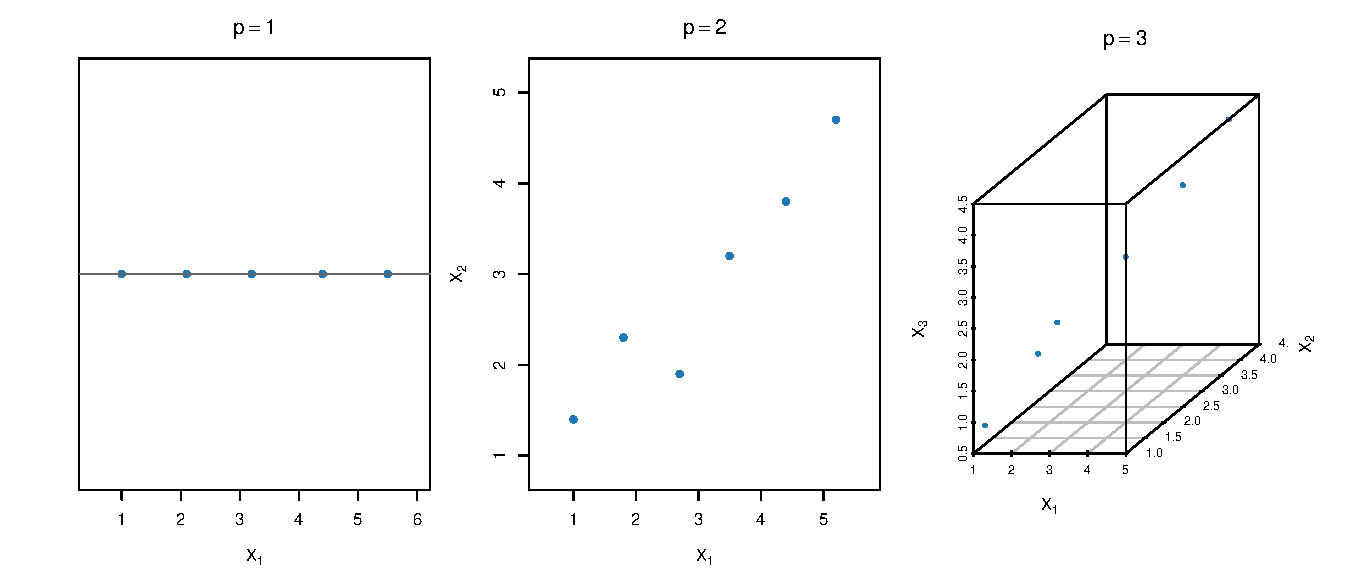
\includegraphics[keepaspectratio]{mod_1_vetores_files/figure-pdf/fig-dimensoes-rp-1.pdf}}

}

\caption{\label{fig-dimensoes-rp}Representação de observações em espaços
de uma, duas e três dimensões.}

\end{figure}%

\begin{example}[Observação em duas
dimensões]\protect\hypertarget{exm-observacao-r2}{}\label{exm-observacao-r2}

Considere duas variáveis quantitativas, \(X_1\) e \(X_2\). A observação
\(i\) é representada por

\[
\mathbf{x}_i
=
\begin{bmatrix}
x_{i1}\\
x_{i2}
\end{bmatrix}
\in\mathbb{R}^2.
\]

Se \(x_{i1}=3\) e \(x_{i2}=5\), então

\[
\mathbf{x}_i
=
\begin{bmatrix}
3\\
5
\end{bmatrix}.
\]

Esse vetor pode ser representado por uma seta que parte da origem e
termina no ponto de coordenadas \((3,5)\), como mostra a
Figura~\ref{fig-vetor-observacao-r2}.

\begin{figure}

\centering{

\pandocbounded{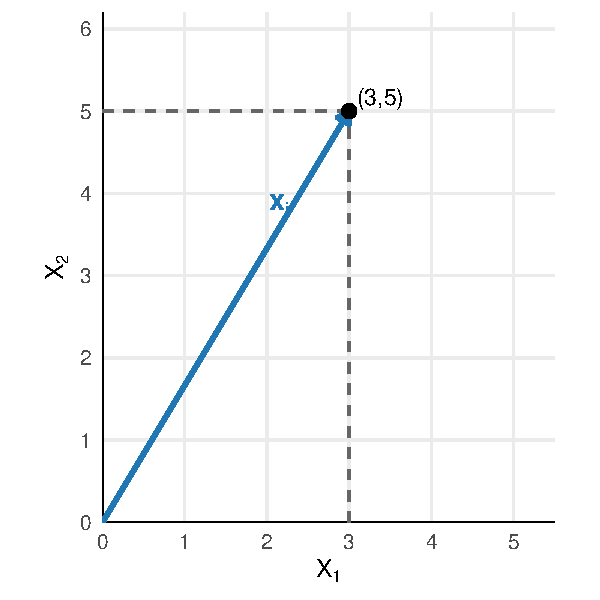
\includegraphics[keepaspectratio]{mod_1_vetores_files/figure-pdf/fig-vetor-observacao-r2-1.pdf}}

}

\caption{\label{fig-vetor-observacao-r2}Representação do vetor
\(\mathbf{x}_i=(3,5)^\top\) no plano.}

\end{figure}%

A extremidade da seta determina o ponto \((3,5)\). Assim, o vetor
\(\mathbf{x}_i\) pode ser interpretado geometricamente como uma seta com
origem em \((0,0)\) e extremidade em \((3,5)\).

\end{example}

O número de observações e o número de variáveis possuem funções
distintas. Para um conjunto com \(n\) observações e \(p\) variáveis:

\begin{itemize}
\tightlist
\item
  \(n\) determina a quantidade de pontos;
\item
  \(p\) determina a dimensão do espaço ambiente.
\end{itemize}

As \(n\) observações formam uma nuvem de pontos em \(\mathbb{R}^p\).

Os vetores correspondentes às \(n\) observações serão organizados em uma
matriz de dados na próxima seção.

\section{Representação matricial de um conjunto de
dados}\label{representauxe7uxe3o-matricial-de-um-conjunto-de-dados}

Considere \(n\) unidades observacionais descritas pelas mesmas \(p\)
variáveis quantitativas. A observação \(i\) é representada pelo vetor

\[
\mathbf{x}_i
=
\begin{bmatrix}
x_{i1}\\
x_{i2}\\
\vdots\\
x_{ip}
\end{bmatrix}
\in
\mathbb{R}^p,
\qquad
i=1,\ldots,n.
\]

Cada componente \(x_{ij}\) corresponde ao valor da variável \(j\)
observado na unidade \(i\). Os \(n\) vetores observados podem ser
organizados nas linhas de uma matriz.

\begin{definition}[Matriz de
dados]\protect\hypertarget{def-matriz-dados}{}\label{def-matriz-dados}

A \textbf{matriz de dados} de \(n\) observações e \(p\) variáveis é
definida por

\[
\mathbf{X}
=
\begin{bmatrix}
x_{11} & x_{12} & \cdots & x_{1p}\\
x_{21} & x_{22} & \cdots & x_{2p}\\
\vdots & \vdots & \ddots & \vdots\\
x_{n1} & x_{n2} & \cdots & x_{np}
\end{bmatrix}
\in
\mathbb{R}^{n\times p}.
\]

O elemento \(x_{ij}\) representa o valor da variável \(j\) observado na
unidade \(i\).

\end{definition}

As linhas da matriz correspondem às observações, e as colunas
correspondem às variáveis. Essa organização coincide com a estrutura
usual de uma planilha ou de um banco de dados.

Com a notação estabelecida anteriormente, a matriz de dados pode ser
representada por suas linhas como

\[
\mathbf{X}
=
\begin{bmatrix}
\mathbf{x}_{1}^{\top}\\
\mathbf{x}_{2}^{\top}\\
\vdots\\
\mathbf{x}_{n}^{\top}
\end{bmatrix},
\]

ou por suas colunas como

\[
\mathbf{X}
=
\left[
\mathbf{x}_{\cdot1}
\;
\mathbf{x}_{\cdot2}
\;
\cdots
\;
\mathbf{x}_{\cdot p}
\right].
\]

\begin{example}[Matriz de dados com duas
variáveis]\protect\hypertarget{exm-matriz-dados}{}\label{exm-matriz-dados}

Considere quatro unidades observacionais descritas pelas variáveis
\(X_1\) e \(X_2\). Os vetores observados são

\[
\mathbf{x}_1
=
\begin{bmatrix}
1\\
5
\end{bmatrix},
\qquad
\mathbf{x}_2
=
\begin{bmatrix}
3\\
1
\end{bmatrix},
\]

\[
\mathbf{x}_3
=
\begin{bmatrix}
5\\
7
\end{bmatrix},
\qquad
\mathbf{x}_4
=
\begin{bmatrix}
8\\
3
\end{bmatrix}.
\]

A matriz de dados é

\[
\mathbf{X}
=
\begin{bmatrix}
1 & 5\\
3 & 1\\
5 & 7\\
8 & 3
\end{bmatrix}
\in
\mathbb{R}^{4\times2}.
\]

A terceira observação é

\[
\mathbf{x}_3
=
\begin{bmatrix}
5\\
7
\end{bmatrix},
\]

e aparece na matriz como a terceira linha,

\[
\mathbf{x}_3^{\top}
=
\begin{bmatrix}
5 & 7
\end{bmatrix}.
\]

O elemento

\[
x_{32}=7
\]

é o valor da segunda variável observado na terceira unidade.

\end{example}

\subsection{Espaço das observações e espaço das
variáveis}\label{espauxe7o-das-observauxe7uxf5es-e-espauxe7o-das-variuxe1veis}

A organização da matriz de dados permite considerar dois conjuntos de
vetores.

Pelas linhas,

\[
\mathbf{x}_{i}
\in
\mathbb{R}^p,
\qquad
i=1,\ldots,n,
\]

cada vetor representa uma observação descrita pelas \(p\) variáveis.

Pelas colunas,

\[
\mathbf{x}_{\cdot j}
\in
\mathbb{R}^n,
\qquad
j=1,\ldots,p,
\]

cada vetor representa uma variável observada nas \(n\) unidades.

No \textbf{espaço das observações}, cada unidade observacional é
representada por um ponto em \(\mathbb{R}^p\), cujas coordenadas
correspondem às variáveis.

No \textbf{espaço das variáveis}, cada variável é representada por um
vetor em \(\mathbb{R}^n\), cujas componentes correspondem às unidades
observacionais.

A Tabela~\ref{tbl-espacos-observacoes-variaveis} resume essas duas
representações.

\begin{longtable}[]{@{}
  >{\raggedright\arraybackslash}p{(\linewidth - 8\tabcolsep) * \real{0.1918}}
  >{\raggedright\arraybackslash}p{(\linewidth - 8\tabcolsep) * \real{0.2329}}
  >{\raggedright\arraybackslash}p{(\linewidth - 8\tabcolsep) * \real{0.1918}}
  >{\centering\arraybackslash}p{(\linewidth - 8\tabcolsep) * \real{0.1918}}
  >{\centering\arraybackslash}p{(\linewidth - 8\tabcolsep) * \real{0.1918}}@{}}
\caption{Representações da matriz de dados por linhas e
colunas.}\label{tbl-espacos-observacoes-variaveis}\tabularnewline
\toprule\noalign{}
\begin{minipage}[b]{\linewidth}\raggedright
Representação
\end{minipage} & \begin{minipage}[b]{\linewidth}\raggedright
Vetor
\end{minipage} & \begin{minipage}[b]{\linewidth}\raggedright
Objeto representado
\end{minipage} & \begin{minipage}[b]{\linewidth}\centering
Espaço
\end{minipage} & \begin{minipage}[b]{\linewidth}\centering
Quantidade
\end{minipage} \\
\midrule\noalign{}
\endfirsthead
\toprule\noalign{}
\begin{minipage}[b]{\linewidth}\raggedright
Representação
\end{minipage} & \begin{minipage}[b]{\linewidth}\raggedright
Vetor
\end{minipage} & \begin{minipage}[b]{\linewidth}\raggedright
Objeto representado
\end{minipage} & \begin{minipage}[b]{\linewidth}\centering
Espaço
\end{minipage} & \begin{minipage}[b]{\linewidth}\centering
Quantidade
\end{minipage} \\
\midrule\noalign{}
\endhead
\bottomrule\noalign{}
\endlastfoot
Linhas de \(\mathbf{X}\) & \(\mathbf{x}_i\) & Observação \(i\) &
\(\mathbb{R}^p\) & \(n\) vetores \\
Colunas de \(\mathbf{X}\) & \(\mathbf{x}_{\cdot j}\) & Variável \(j\) &
\(\mathbb{R}^n\) & \(p\) vetores \\
\end{longtable}

A interpretação utilizada depende do objeto de interesse. Relações entre
unidades observacionais são estudadas a partir das linhas da matriz,
enquanto relações entre variáveis são estudadas a partir de suas
colunas.

\section{Operações elementares com
vetores}\label{operauxe7uxf5es-elementares-com-vetores}

Considere os vetores

\[
\mathbf{x}
=
\begin{bmatrix}
x_1\\
x_2\\
\vdots\\
x_p
\end{bmatrix},
\qquad
\mathbf{y}
=
\begin{bmatrix}
y_1\\
y_2\\
\vdots\\
y_p
\end{bmatrix}
\in\mathbb{R}^p
\]

e um escalar \(\alpha\in\mathbb{R}\).

Dois vetores são iguais quando suas componentes correspondentes são
iguais:

\[
\mathbf{x}=\mathbf{y}
\quad\Longleftrightarrow\quad
x_j=y_j,
\qquad
j=1,\ldots,p.
\]

\subsection{Soma e subtração}\label{soma-e-subtrauxe7uxe3o}

A soma de dois vetores é realizada componente a componente:

\[
\mathbf{x}+\mathbf{y}
=
\begin{bmatrix}
x_1+y_1\\
x_2+y_2\\
\vdots\\
x_p+y_p
\end{bmatrix}
\in\mathbb{R}^p.
\]

A diferença também é calculada componente a componente:

\[
\mathbf{x}-\mathbf{y}
=
\begin{bmatrix}
x_1-y_1\\
x_2-y_2\\
\vdots\\
x_p-y_p
\end{bmatrix}
\in\mathbb{R}^p.
\]

O vetor \(\mathbf{x}-\mathbf{y}\) representa o deslocamento de
\(\mathbf{y}\) até \(\mathbf{x}\).

\begin{example}[Soma e subtração de
vetores]\protect\hypertarget{exm-soma-subtracao}{}\label{exm-soma-subtracao}

Considere

\[
\mathbf{x}
=
\begin{bmatrix}
2{,}0\\
1{,}5
\end{bmatrix},
\qquad
\mathbf{y}
=
\begin{bmatrix}
1{,}0\\
3{,}0
\end{bmatrix}.
\]

A soma é

\[
\mathbf{x}+\mathbf{y}
=
\begin{bmatrix}
2{,}0+1{,}0\\
1{,}5+3{,}0
\end{bmatrix}
=
\begin{bmatrix}
3{,}0\\
4{,}5
\end{bmatrix}.
\]

A diferença é

\[
\mathbf{x}-\mathbf{y}
=
\begin{bmatrix}
2{,}0-1{,}0\\
1{,}5-3{,}0
\end{bmatrix}
=
\begin{bmatrix}
1{,}0\\
-1{,}5
\end{bmatrix}.
\]

\end{example}

\begin{definition}[Vetor
nulo]\protect\hypertarget{def-vetor-nulo}{}\label{def-vetor-nulo}

O \textbf{vetor nulo} de \(\mathbb{R}^p\) é definido por

\[
\mathbf{0}
=
\begin{bmatrix}
0\\
0\\
\vdots\\
0
\end{bmatrix}.
\]

Ele é o elemento neutro da adição:

\[
\mathbf{x}+\mathbf{0}
=
\mathbf{x}.
\]

\end{definition}

A Figura~\ref{fig-soma-vetores} apresenta a interpretação geométrica da
soma em \(\mathbb{R}^2\).

\begin{figure}

\centering{

\pandocbounded{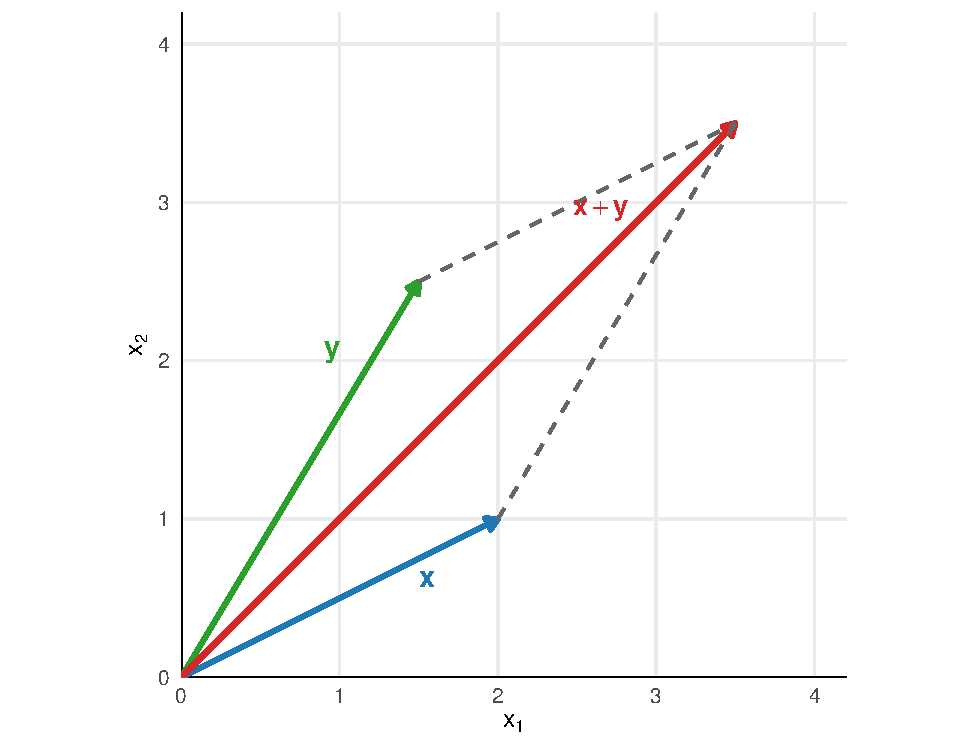
\includegraphics[keepaspectratio]{mod_1_vetores_files/figure-pdf/fig-soma-vetores-1.pdf}}

}

\caption{\label{fig-soma-vetores}Soma de vetores pela regra do
paralelogramo.}

\end{figure}%

Na figura, os vetores \(\mathbf{x}\) e \(\mathbf{y}\) formam dois lados
de um paralelogramo. A diagonal que parte da origem representa
\(\mathbf{x}+\mathbf{y}\).

\subsection{Multiplicação por
escalar}\label{multiplicauxe7uxe3o-por-escalar}

A multiplicação do vetor \(\mathbf{x}\) pelo escalar \(\alpha\) é
definida por

\[
\alpha\mathbf{x}
=
\begin{bmatrix}
\alpha x_1\\
\alpha x_2\\
\vdots\\
\alpha x_p
\end{bmatrix}
\in\mathbb{R}^p.
\]

A norma do vetor resultante satisfaz

\[
\|\alpha\mathbf{x}\|
=
|\alpha|\,\|\mathbf{x}\|.
\]

Portanto, para \(\mathbf{x}\neq\mathbf{0}\):

\begin{itemize}
\tightlist
\item
  se \(|\alpha|>1\), o comprimento do vetor aumenta;
\item
  se \(0<|\alpha|<1\), o comprimento do vetor diminui;
\item
  se \(|\alpha|=1\), o comprimento do vetor é preservado;
\item
  se \(\alpha=0\), o resultado é o vetor nulo;
\item
  se \(\alpha<0\), o sentido do vetor é invertido.
\end{itemize}

As alterações de comprimento dependem de \(|\alpha|\), enquanto a
inversão do sentido depende do sinal de \(\alpha\). Assim, um escalar
negativo pode aumentar, diminuir ou preservar o comprimento do vetor.

Quando \(\mathbf{x}=\mathbf{0}\), tem-se

\[
\alpha\mathbf{x}
=
\mathbf{0}
\]

para qualquer \(\alpha\in\mathbb{R}\).

\begin{example}[Multiplicação por
escalar]\protect\hypertarget{exm-multiplicacao-escalar}{}\label{exm-multiplicacao-escalar}

Para

\[
\mathbf{x}
=
\begin{bmatrix}
2{,}0\\
-1{,}5
\end{bmatrix}
\]

e \(\alpha=-2\), tem-se

\[
-2\mathbf{x}
=
\begin{bmatrix}
-2(2{,}0)\\
-2(-1{,}5)
\end{bmatrix}
=
\begin{bmatrix}
-4{,}0\\
3{,}0
\end{bmatrix}.
\]

\end{example}

\subsection{Combinações lineares}\label{combinauxe7uxf5es-lineares}

Uma combinação linear é construída por meio das duas operações
apresentadas anteriormente: a multiplicação de vetores por escalares e a
adição de vetores.

\begin{definition}[Combinação linear de
vetores]\protect\hypertarget{def-combinacao-linear}{}\label{def-combinacao-linear}

Sejam

\[
\mathbf{v}_1,\mathbf{v}_2,\ldots,\mathbf{v}_k
\in\mathbb{R}^p
\]

e

\[
\alpha_1,\alpha_2,\ldots,\alpha_k
\in\mathbb{R}.
\]

Uma \textbf{combinação linear} dos vetores
\(\mathbf{v}_1,\ldots,\mathbf{v}_k\) é qualquer vetor da forma

\[
\alpha_1\mathbf{v}_1
+
\alpha_2\mathbf{v}_2
+
\cdots
+
\alpha_k\mathbf{v}_k.
\]

\end{definition}

O resultado também pertence a \(\mathbb{R}^p\), pois é obtido por
multiplicações por escalares e somas de vetores de \(\mathbb{R}^p\):

\[
\alpha_1\mathbf{v}_1
+
\cdots
+
\alpha_k\mathbf{v}_k
\in\mathbb{R}^p.
\]

\begin{example}[Combinação linear de
vetores]\protect\hypertarget{exm-combinacao-vetores}{}\label{exm-combinacao-vetores}

Considere

\[
\mathbf{v}_1
=
\begin{bmatrix}
1\\
2
\end{bmatrix}
\qquad\text{e}\qquad
\mathbf{v}_2
=
\begin{bmatrix}
3\\
-1
\end{bmatrix}.
\]

A combinação linear \(2\mathbf{v}_1-\mathbf{v}_2\) é

\[
2\mathbf{v}_1-\mathbf{v}_2
=
2
\begin{bmatrix}
1\\
2
\end{bmatrix}
-
\begin{bmatrix}
3\\
-1
\end{bmatrix}
=
\begin{bmatrix}
-1\\
5
\end{bmatrix}.
\]

\end{example}

As combinações lineares permitem construir novos vetores a partir de
vetores já conhecidos. Seus coeficientes determinam quanto cada vetor
contribui para o resultado.

\begin{example}[Combinação linear das
variáveis]\protect\hypertarget{exm-combinacao-variaveis}{}\label{exm-combinacao-variaveis}

Considere as variáveis \(X_1\), \(X_2\) e \(X_3\) e os coeficientes

\[
a_1=2{,}0,
\qquad
a_2=-0{,}5,
\qquad
a_3=3{,}0.
\]

A combinação linear definida por esses coeficientes é

\[
Y
=
2{,}0X_1
-
0{,}5X_2
+
3{,}0X_3.
\]

Para uma observação com valores

\[
x_1=4{,}0,
\qquad
x_2=2{,}0,
\qquad
x_3=1{,}5,
\]

o valor observado da combinação linear é

\[
y
=
2{,}0(4{,}0)
-
0{,}5(2{,}0)
+
3{,}0(1{,}5)
=
11{,}5.
\]

\end{example}

Em uma combinação linear, cada coeficiente determina a contribuição do
vetor ou da variável correspondente para o resultado.

As operações anteriores produzem novos vetores ou novas variáveis. A
próxima operação tem natureza diferente: o produto interno associa dois
vetores a um número real e permite construir as noções de comprimento,
ângulo, ortogonalidade e distância.

\section{Produto interno, norma, ângulo e distância
euclidiana}\label{produto-interno-norma-uxe2ngulo-e-distuxe2ncia-euclidiana}

O produto interno associa dois vetores de \(\mathbb{R}^p\) a um número
real. A partir dessa operação, definem-se norma, ângulo, ortogonalidade
e distância euclidiana.

\subsection{Produto interno
euclidiano}\label{produto-interno-euclidiano}

\begin{definition}[Produto interno
euclidiano]\protect\hypertarget{def-produto-interno-euclidiano}{}\label{def-produto-interno-euclidiano}

Para \(\mathbf{x},\mathbf{y}\in\mathbb{R}^p\), o \textbf{produto interno
euclidiano} entre \(\mathbf{x}\) e \(\mathbf{y}\) é definido por

\[
\langle \mathbf{x},\mathbf{y}\rangle
=
\sum_{j=1}^{p}x_jy_j.
\]

Em termos das componentes,

\[
\langle \mathbf{x},\mathbf{y}\rangle
=
x_1y_1+x_2y_2+\cdots+x_py_p.
\]

O resultado do produto interno é um escalar.

\end{definition}

\begin{example}[Cálculo do produto
interno]\protect\hypertarget{exm-produto-interno}{}\label{exm-produto-interno}

Considere

\[
\mathbf{x}
=
\begin{bmatrix}
2\\
1\\
3
\end{bmatrix},
\qquad
\mathbf{y}
=
\begin{bmatrix}
4\\
2\\
-1
\end{bmatrix}.
\]

Então,

\[
\langle \mathbf{x},\mathbf{y}\rangle 
=
2(4)+1(2)+3(-1)
=
7.
\]

\end{example}

\begin{proposition}[Propriedades do produto interno
euclidiano]\protect\hypertarget{prp-propriedades-produto-interno}{}\label{prp-propriedades-produto-interno}

Para quaisquer vetores
\(\mathbf{x},\mathbf{y},\mathbf{z}\in\mathbb{R}^p\) e quaisquer
escalares \(\alpha,\beta\in\mathbb{R}\), o produto interno euclidiano
satisfaz as seguintes propriedades:

\begin{enumerate}
\def\labelenumi{\arabic{enumi}.}
\item
  \textbf{Simetria}

  \[
  \langle\mathbf{x},\mathbf{y}\rangle
  =
  \langle\mathbf{y},\mathbf{x}\rangle.
  \]
\item
  \textbf{Linearidade no primeiro argumento}

  \[
  \left\langle
  \alpha\mathbf{x}+\beta\mathbf{z},
  \mathbf{y}
  \right\rangle
  =
  \alpha\langle\mathbf{x},\mathbf{y}\rangle
  +
  \beta\langle\mathbf{z},\mathbf{y}\rangle.
  \]
\item
  \textbf{Linearidade no segundo argumento}

  \[
  \left\langle
  \mathbf{x},
  \alpha\mathbf{y}+\beta\mathbf{z}
  \right\rangle
  =
  \alpha\langle\mathbf{x},\mathbf{y}\rangle
  +
  \beta\langle\mathbf{x},\mathbf{z}\rangle.
  \]
\item
  \textbf{Não negatividade}

  \[
  \langle\mathbf{x},\mathbf{x}\rangle
  \geq 0.
  \]
\item
  \textbf{Positividade definida}

  \[
  \langle\mathbf{x},\mathbf{x}\rangle
  =
  0
  \quad\Longleftrightarrow\quad
  \mathbf{x}=\mathbf{0}.
  \]
\end{enumerate}

\end{proposition}

\subsection{Norma euclidiana}\label{norma-euclidiana}

\begin{definition}[Norma
euclidiana]\protect\hypertarget{def-norma-euclidiana}{}\label{def-norma-euclidiana}

A \textbf{norma euclidiana} de \(\mathbf{x}\in\mathbb{R}^p\) é definida
por

\[
\|\mathbf{x}\| = \sqrt{\langle \mathbf{x},\mathbf{x}\rangle} = \sqrt{x_1^2+x_2^2+\cdots+x_p^2}.
\]

\end{definition}

A norma representa o comprimento do vetor em relação à origem.

Para qualquer \(\mathbf{x}\in\mathbb{R}^p\) e \(\alpha\in\mathbb{R}\),

\[
\|\mathbf{x}\|
\geq
0,
\]

\[
\|\mathbf{x}\|
=
0
\quad\Longleftrightarrow\quad
\mathbf{x}
=
\mathbf{0},
\]

e

\[
\|\alpha\mathbf{x}\|
=
|\alpha|\|\mathbf{x}\|.
\]

\begin{example}[Norma de um
vetor]\protect\hypertarget{exm-norma-euclidiana}{}\label{exm-norma-euclidiana}

Para

\[
\mathbf{x}
=
\begin{bmatrix}
3\\
4
\end{bmatrix},
\]

tem-se

\[
\|\mathbf{x}\|
=
\sqrt{3^2+4^2}
=
5.
\]

A Figura~\ref{fig-norma-vetor} mostra a representação geométrica desse
vetor no plano. O comprimento da seta corresponde à norma euclidiana do
vetor.

\begin{figure}

\centering{

\pandocbounded{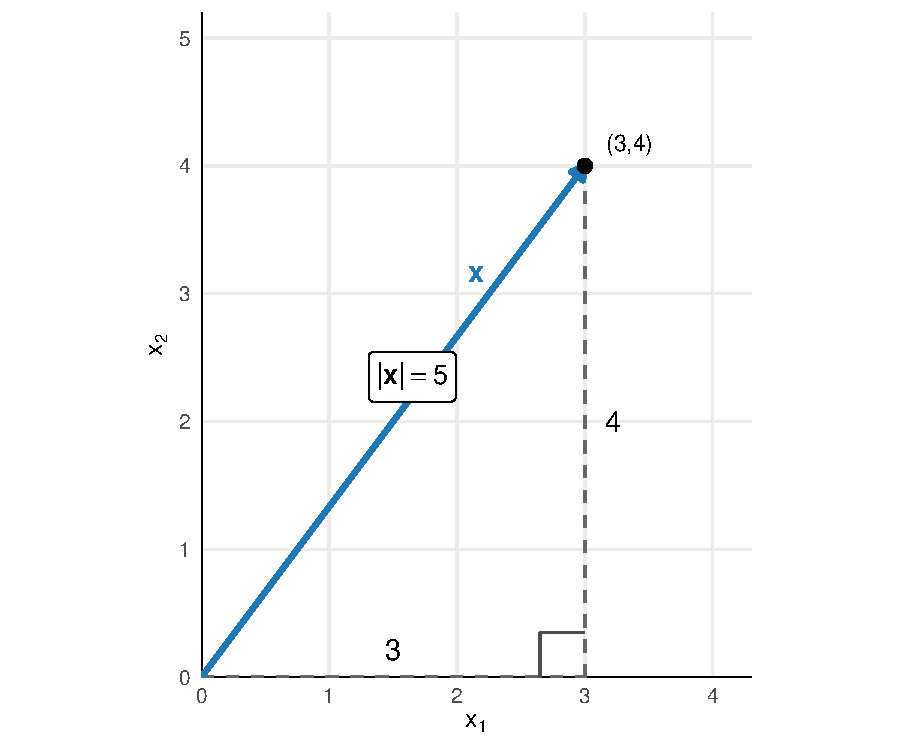
\includegraphics[keepaspectratio]{mod_1_vetores_files/figure-pdf/fig-norma-vetor-1.pdf}}

}

\caption{\label{fig-norma-vetor}A norma euclidiana corresponde ao
comprimento do vetor.}

\end{figure}%

Nesse caso, a norma coincide com a hipotenusa de um triângulo retângulo
cujos catetos têm comprimentos \(3\) e \(4\).

\end{example}

\subsection{Desigualdade de
Cauchy--Schwarz}\label{desigualdade-de-cauchyschwarz}

\begin{theorem}[Desigualdade de
Cauchy--Schwarz]\protect\hypertarget{thm-cauchy-schwarz}{}\label{thm-cauchy-schwarz}

Para quaisquer vetores \(\mathbf{x},\mathbf{y}\in\mathbb{R}^p\),

\[
\left|
\langle\mathbf{x},\mathbf{y}\rangle
\right|
\leq
\|\mathbf{x}\|\,\|\mathbf{y}\|.
\]

A igualdade ocorre se, e somente se, um dos vetores é múltiplo escalar
do outro. (Meyer, 2023)

\end{theorem}

\begin{proof}
Se \(\mathbf{y}=\mathbf{0}\), então

\[
\langle\mathbf{x},\mathbf{y}\rangle=0
\]

e

\[
\|\mathbf{x}\|\,\|\mathbf{y}\|=0.
\]

Portanto, a desigualdade é satisfeita com igualdade. Além disso,

\[
\mathbf{y}=0\mathbf{x},
\]

de modo que um dos vetores é múltiplo escalar do outro.

Considere agora \(\mathbf{y}\neq\mathbf{0}\). Para qualquer escalar
\(\alpha\in\mathbb{R}\), a não negatividade do produto interno implica

\[
\left\langle
\mathbf{x}-\alpha\mathbf{y},
\mathbf{x}-\alpha\mathbf{y}
\right\rangle
\geq 0.
\]

Escolha

\[
\alpha
=
\frac{
\langle\mathbf{x},\mathbf{y}\rangle
}{
\|\mathbf{y}\|^2
}.
\]

Expandindo o produto interno,

\[
\begin{aligned}
0
&\leq
\left\langle
\mathbf{x}-\alpha\mathbf{y},
\mathbf{x}-\alpha\mathbf{y}
\right\rangle\\
&=
\langle\mathbf{x},\mathbf{x}\rangle
-
\alpha\langle\mathbf{x},\mathbf{y}\rangle
-
\alpha\langle\mathbf{y},\mathbf{x}\rangle
+
\alpha^2\langle\mathbf{y},\mathbf{y}\rangle\\
&=
\|\mathbf{x}\|^2
-
2\alpha\langle\mathbf{x},\mathbf{y}\rangle
+
\alpha^2\|\mathbf{y}\|^2.
\end{aligned}
\]

Na última igualdade, foi utilizada a simetria do produto interno:

\[
\langle\mathbf{x},\mathbf{y}\rangle
=
\langle\mathbf{y},\mathbf{x}\rangle.
\]

Substituindo o valor escolhido para \(\alpha\),

\[
\begin{aligned}
0
&\leq
\|\mathbf{x}\|^2
-
2
\frac{
\langle\mathbf{x},\mathbf{y}\rangle
}{
\|\mathbf{y}\|^2
}
\langle\mathbf{x},\mathbf{y}\rangle\\
&\quad+
\left(
\frac{
\langle\mathbf{x},\mathbf{y}\rangle
}{
\|\mathbf{y}\|^2
}
\right)^2
\|\mathbf{y}\|^2\\
&=
\|\mathbf{x}\|^2
-
\frac{
\langle\mathbf{x},\mathbf{y}\rangle^2
}{
\|\mathbf{y}\|^2
}.
\end{aligned}
\]

Logo,

\[
\frac{
\langle\mathbf{x},\mathbf{y}\rangle^2
}{
\|\mathbf{y}\|^2
}
\leq
\|\mathbf{x}\|^2.
\]

Como \(\|\mathbf{y}\|^2>0\), podemos multiplicar os dois lados por esse
valor e obter

\[
\langle\mathbf{x},\mathbf{y}\rangle^2
\leq
\|\mathbf{x}\|^2\|\mathbf{y}\|^2.
\]

Tomando a raiz quadrada dos dois lados,

\[
\left|
\langle\mathbf{x},\mathbf{y}\rangle
\right|
\leq
\|\mathbf{x}\|\,\|\mathbf{y}\|.
\]

Resta examinar quando ocorre a igualdade. Na construção anterior, a
igualdade é satisfeita se, e somente se,

\[
\left\langle
\mathbf{x}-\alpha\mathbf{y},
\mathbf{x}-\alpha\mathbf{y}
\right\rangle
=
0.
\]

Pela positividade definida do produto interno, isso ocorre se, e somente
se,

\[
\mathbf{x}-\alpha\mathbf{y}
=
\mathbf{0},
\]

ou seja,

\[
\mathbf{x}
=
\alpha\mathbf{y}.
\]

Portanto, quando \(\mathbf{y}\neq\mathbf{0}\), a igualdade ocorre se, e
somente se, \(\mathbf{x}\) é múltiplo escalar de \(\mathbf{y}\).

Reunindo os dois casos, concluímos que a igualdade ocorre se, e somente
se, um dos vetores é múltiplo escalar do outro.
\end{proof}

Para vetores não nulos, a desigualdade de Cauchy--Schwarz também implica

\[
-1
\leq
\frac{
\langle\mathbf{x},\mathbf{y}\rangle
}{
\|\mathbf{x}\|\,\|\mathbf{y}\|
}
\leq
1.
\]

Assim, a desigualdade fornece uma justificativa algébrica de que a razão
utilizada no cálculo do ângulo pertence ao intervalo \([-1,1]\), que é o
domínio da função \(\arccos\).

\subsection{Ângulo entre vetores}\label{uxe2ngulo-entre-vetores}

\begin{definition}[Ângulo entre
vetores]\protect\hypertarget{def-angulo-vetores}{}\label{def-angulo-vetores}

Para \(\mathbf{x},\mathbf{y}\in\mathbb{R}^p\) não nulos, o
\textbf{ângulo} entre os vetores é o único valor \(\theta\in[0,\pi]\)
que satisfaz

\[
\cos(\theta)
=
\frac{
\langle\mathbf{x},\mathbf{y}\rangle
}{
\|\mathbf{x}\|\,\|\mathbf{y}\|
}.
\]

A existência desse ângulo é garantida pela desigualdade de
Cauchy--Schwarz, pois

\[
-1
\leq
\frac{
\langle\mathbf{x},\mathbf{y}\rangle
}{
\|\mathbf{x}\|\,\|\mathbf{y}\|
}
\leq
1.
\]

Equivalentemente,

\[
\theta
=
\arccos
\left(
\frac{
\langle\mathbf{x},\mathbf{y}\rangle
}{
\|\mathbf{x}\|\,\|\mathbf{y}\|
}
\right).
\]

\end{definition}

A relação que define o ângulo também pode ser escrita como

\[
\langle\mathbf{x},\mathbf{y}\rangle
=
\|\mathbf{x}\|\,\|\mathbf{y}\|\cos(\theta).
\]

\textbf{Interpretação geométrica}

A divisão pelo produto das normas retira o efeito dos comprimentos dos
vetores. Desse modo, o valor de \(\cos(\theta)\) descreve apenas o
alinhamento entre suas direções.

Como \(\|\mathbf{x}\|\) e \(\|\mathbf{y}\|\) são positivos, o sinal do
produto interno depende apenas do sinal de \(\cos(\theta)\):

\begin{itemize}
\item
  se \(0\leq\theta<\dfrac{\pi}{2}\), o ângulo é agudo e

  \[
  \langle\mathbf{x},\mathbf{y}\rangle>0;
  \]
\item
  se \(\theta=\dfrac{\pi}{2}\), o ângulo é reto e

  \[
  \langle\mathbf{x},\mathbf{y}\rangle=0;
  \]
\item
  se \(\dfrac{\pi}{2}<\theta\leq\pi\), o ângulo é obtuso e

  \[
  \langle\mathbf{x},\mathbf{y}\rangle<0.
  \]
\end{itemize}

Geometricamente, o produto interno é positivo quando os vetores apontam
para direções relativamente próximas, é nulo quando são ortogonais e é
negativo quando apontam para direções relativamente opostas.

O ângulo não é definido quando um dos vetores é nulo, pois o vetor nulo
não possui direção determinada e o denominador da expressão seria igual
a zero.

A Figura~\ref{fig-produto-interno} apresenta essas três situações.

\begin{figure}

\centering{

\pandocbounded{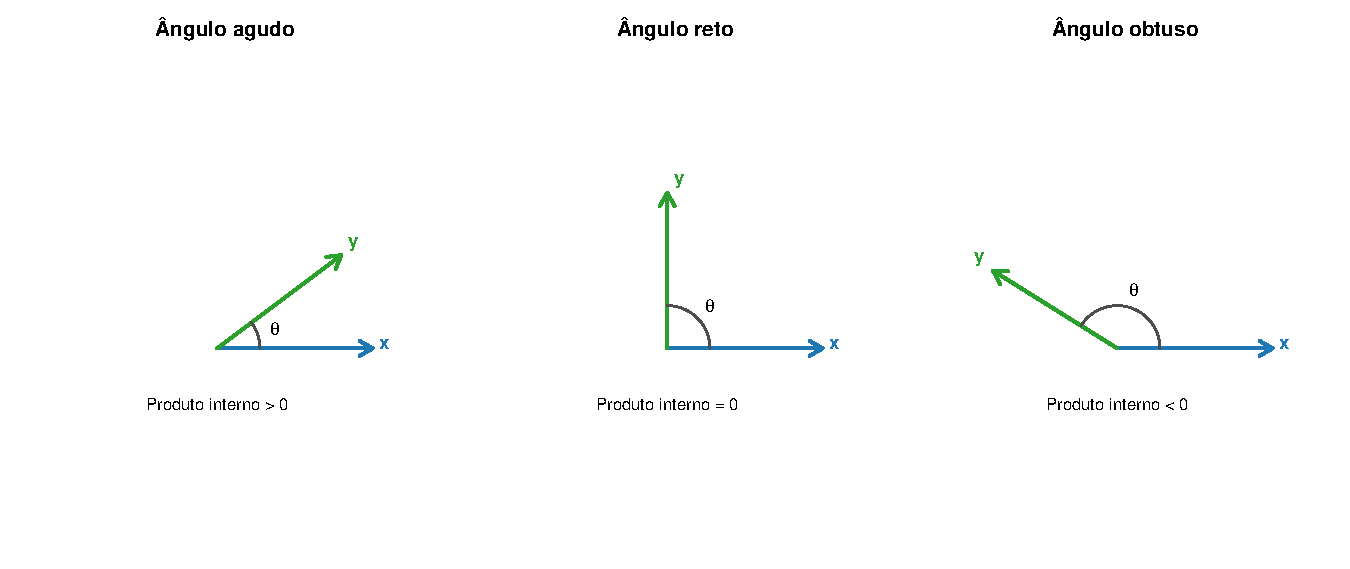
\includegraphics[keepaspectratio]{mod_1_vetores_files/figure-pdf/fig-produto-interno-1.pdf}}

}

\caption{\label{fig-produto-interno}Sinal do produto interno segundo o
ângulo formado entre dois vetores.}

\end{figure}%

\begin{definition}[Vetores
ortogonais]\protect\hypertarget{def-ortogonalidade}{}\label{def-ortogonalidade}

Dois vetores \(\mathbf{x},\mathbf{y}\in\mathbb{R}^p\) são
\textbf{ortogonais} quando

\[
\langle \mathbf{x},\mathbf{y}\rangle
=
0.
\]

Se ambos forem não nulos, o ângulo entre eles é igual a \(90^\circ\).

\end{definition}

O vetor nulo é ortogonal a todos os vetores, pois

\[
\langle \mathbf{0},\mathbf{x}\rangle
=
0.
\]

O ângulo entre o vetor nulo e outro vetor não é definido porque
\(\|\mathbf{0}\|=0\).

\subsection{Distância euclidiana}\label{distuxe2ncia-euclidiana}

\begin{definition}[Distância
euclidiana]\protect\hypertarget{def-distancia-euclidiana}{}\label{def-distancia-euclidiana}

A \textbf{distância euclidiana} entre
\(\mathbf{x},\mathbf{y}\in\mathbb{R}^p\) é definida por

\[
d_E(\mathbf{x},\mathbf{y})
=
\|\mathbf{x}-\mathbf{y}\|.
\]

Em termos das componentes,

\[
d_E(\mathbf{x},\mathbf{y})
=
\sqrt{
\sum_{j=1}^{p}
(x_j-y_j)^2
}.
\]

\end{definition}

A distância euclidiana corresponde ao comprimento do segmento que liga
os pontos representados por \(\mathbf{x}\) e \(\mathbf{y}\).

\begin{example}[Distância entre duas
observações]\protect\hypertarget{exm-distancia-euclidiana}{}\label{exm-distancia-euclidiana}

Considere

\[
\mathbf{x}
=
\begin{bmatrix}
2\\
1
\end{bmatrix},
\qquad
\mathbf{y}
=
\begin{bmatrix}
5\\
5
\end{bmatrix}.
\]

A diferença entre os vetores é

\[
\mathbf{x}-\mathbf{y}
=
\begin{bmatrix}
-3\\
-4
\end{bmatrix}.
\]

Logo,

\[
d_E(\mathbf{x},\mathbf{y})
=
\sqrt{(-3)^2+(-4)^2}
=
5.
\]

\begin{figure}

\centering{

\pandocbounded{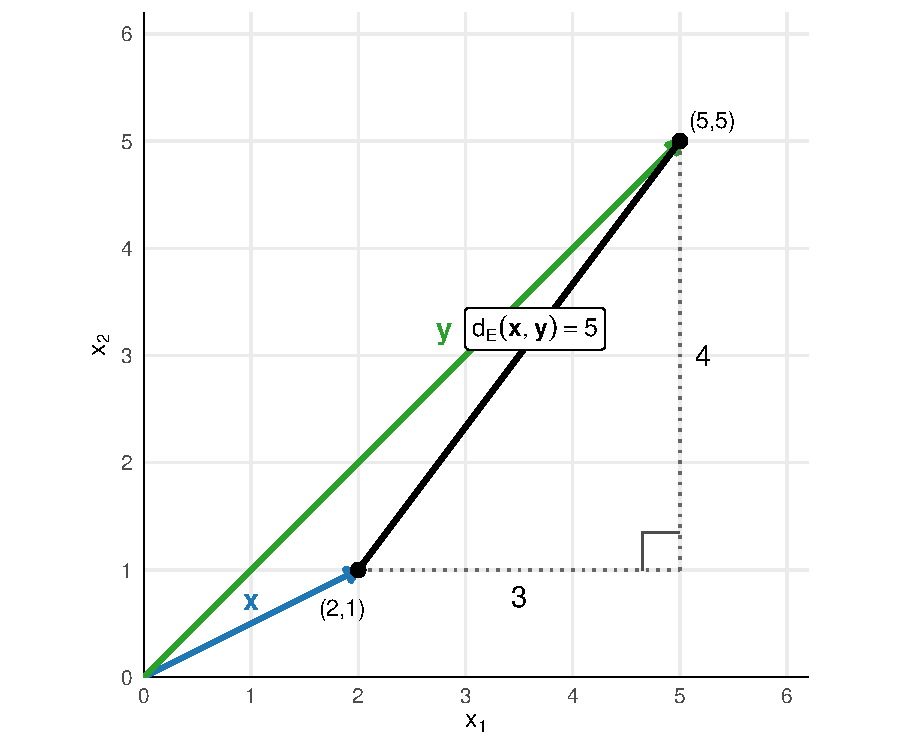
\includegraphics[keepaspectratio]{mod_1_vetores_files/figure-pdf/fig-distancia-euclidiana-1.pdf}}

}

\caption{\label{fig-distancia-euclidiana}Os vetores \(\mathbf{x}\) e
\(\mathbf{y}\) são representados por setas. A distância euclidiana é o
comprimento do segmento que une suas extremidades.}

\end{figure}%

\end{example}

\begin{tcolorbox}[enhanced jigsaw, colback=white, breakable, bottomrule=.15mm, left=2mm, arc=.35mm, rightrule=.15mm, colframe=quarto-callout-caution-color-frame, toprule=.15mm, leftrule=.75mm, opacityback=0]

\vspace{-3mm}\textbf{Escalas das variáveis}\vspace{3mm}

A distância euclidiana depende das unidades e das escalas das variáveis.
Uma variável com valores numericamente maiores pode contribuir mais para
a distância entre as observações. A padronização e outras geometrias
serão estudadas nos capítulos posteriores.

\end{tcolorbox}

\subsection{Desigualdade triangular}\label{desigualdade-triangular}

\begin{theorem}[Desigualdade
triangular]\protect\hypertarget{thm-desigualdade-triangular}{}\label{thm-desigualdade-triangular}

Para quaisquer vetores \(\mathbf{x},\mathbf{y}\in\mathbb{R}^p\),

\[
\|\mathbf{x}+\mathbf{y}\|
\leq
\|\mathbf{x}\|
+
\|\mathbf{y}\|.
\]

Consequentemente, para quaisquer pontos
\(\mathbf{x},\mathbf{y},\mathbf{z}\in\mathbb{R}^p\),

\[
d_E(\mathbf{x},\mathbf{z})
\leq
d_E(\mathbf{x},\mathbf{y})
+
d_E(\mathbf{y},\mathbf{z}).
\]

(Meyer, 2023)

\end{theorem}

\begin{proof}
Pela definição da norma euclidiana,

\[
\|\mathbf{x}+\mathbf{y}\|^2
=
\left\langle
\mathbf{x}+\mathbf{y},
\mathbf{x}+\mathbf{y}
\right\rangle.
\]

Usando a linearidade e a simetria do produto interno,

\[
\begin{aligned}
\|\mathbf{x}+\mathbf{y}\|^2
&=
\langle\mathbf{x},\mathbf{x}\rangle
+
\langle\mathbf{x},\mathbf{y}\rangle
+
\langle\mathbf{y},\mathbf{x}\rangle
+
\langle\mathbf{y},\mathbf{y}\rangle\\
&=
\|\mathbf{x}\|^2
+
2\langle\mathbf{x},\mathbf{y}\rangle
+
\|\mathbf{y}\|^2.
\end{aligned}
\]

Pela desigualdade de Cauchy--Schwarz,

\[
\langle\mathbf{x},\mathbf{y}\rangle
\leq
\left|
\langle\mathbf{x},\mathbf{y}\rangle
\right|
\leq
\|\mathbf{x}\|\,\|\mathbf{y}\|.
\]

Portanto,

\[
\begin{aligned}
\|\mathbf{x}+\mathbf{y}\|^2
&\leq
\|\mathbf{x}\|^2
+
2\|\mathbf{x}\|\,\|\mathbf{y}\|
+
\|\mathbf{y}\|^2\\
&=
\left(
\|\mathbf{x}\|
+
\|\mathbf{y}\|
\right)^2.
\end{aligned}
\]

Como ambos os lados são não negativos, podemos tomar a raiz quadrada e
obter

\[
\|\mathbf{x}+\mathbf{y}\|
\leq
\|\mathbf{x}\|
+
\|\mathbf{y}\|.
\]

Para demonstrar a desigualdade triangular da distância euclidiana,
observe que

\[
\mathbf{x}-\mathbf{z}
=
(\mathbf{x}-\mathbf{y})
+
(\mathbf{y}-\mathbf{z}).
\]

Aplicando a desigualdade triangular da norma,

\[
\|\mathbf{x}-\mathbf{z}\|
\leq
\|\mathbf{x}-\mathbf{y}\|
+
\|\mathbf{y}-\mathbf{z}\|.
\]

Como

\[
d_E(\mathbf{u},\mathbf{v})
=
\|\mathbf{u}-\mathbf{v}\|,
\]

segue que

\[
d_E(\mathbf{x},\mathbf{z})
\leq
d_E(\mathbf{x},\mathbf{y})
+
d_E(\mathbf{y},\mathbf{z}).
\]
\end{proof}

O produto interno, em conjunto com as normas, determina o ângulo entre
vetores. A norma mede o comprimento de um vetor, e a distância
euclidiana mede a separação entre dois pontos. Esses conceitos completam
a representação geométrica inicial dos dados multivariados.

\subsection{Produto externo}\label{produto-externo}

O produto interno associa dois vetores de mesma dimensão a um escalar.
Dois vetores também podem ser utilizados para construir uma matriz por
meio do \textbf{produto externo}.

\begin{definition}[Produto
externo]\protect\hypertarget{def-produto-externo}{}\label{def-produto-externo}

Para \(\mathbf{x}\in\mathbb{R}^p\) e \(\mathbf{y}\in\mathbb{R}^q\), o
\textbf{produto externo} de \(\mathbf{x}\) e \(\mathbf{y}\), denotado
por

\[
\operatorname{ext}(\mathbf{x},\mathbf{y}),
\]

é definido como a matriz em \(\mathbb{R}^{p\times q}\)

\[
\operatorname{ext}(\mathbf{x},\mathbf{y})
=
\begin{bmatrix}
x_1y_1 & x_1y_2 & \cdots & x_1y_q\\
x_2y_1 & x_2y_2 & \cdots & x_2y_q\\
\vdots & \vdots & \ddots & \vdots\\
x_py_1 & x_py_2 & \cdots & x_py_q
\end{bmatrix}.
\]

O elemento localizado na linha \(i\) e na coluna \(j\) é

\[
\left[
\operatorname{ext}(\mathbf{x},\mathbf{y})
\right]_{ij}
=
x_i y_j.
\]

O resultado do produto externo é uma matriz.

\end{definition}

A estrutura do produto externo pode ser observada por suas colunas. Como

\[
\operatorname{ext}(\mathbf{x},\mathbf{y})
=
\begin{bmatrix}
y_1\mathbf{x}
&
y_2\mathbf{x}
&
\cdots
&
y_q\mathbf{x}
\end{bmatrix},
\]

cada coluna é um múltiplo escalar de \(\mathbf{x}\).

Equivalentemente, considerando as linhas,

\[
\operatorname{ext}(\mathbf{x},\mathbf{y})
=
\begin{bmatrix}
x_1\mathbf{y}^{\top}\\
x_2\mathbf{y}^{\top}\\
\vdots\\
x_p\mathbf{y}^{\top}
\end{bmatrix},
\]

de modo que cada linha é um múltiplo escalar de \(\mathbf{y}^{\top}\).

\begin{example}[Produto externo de dois
vetores]\protect\hypertarget{exm-produto-externo}{}\label{exm-produto-externo}

Considere

\[
\mathbf{x}
=
\begin{bmatrix}
1\\
2
\end{bmatrix}
\in
\mathbb{R}^{2}
\]

e

\[
\mathbf{y}
=
\begin{bmatrix}
3\\
-1\\
4
\end{bmatrix}
\in
\mathbb{R}^{3}.
\]

O produto externo é

\[
\begin{aligned}
\operatorname{ext}(\mathbf{x},\mathbf{y})
&=
\begin{bmatrix}
1(3) & 1(-1) & 1(4)\\
2(3) & 2(-1) & 2(4)
\end{bmatrix}\\
&=
\begin{bmatrix}
3 & -1 & 4\\
6 & -2 & 8
\end{bmatrix}.
\end{aligned}
\]

O resultado possui dimensão \(2\times3\), correspondente às dimensões de
\(\mathbf{x}\) e \(\mathbf{y}\), respectivamente.

\end{example}

O produto interno e o produto externo produzem objetos de naturezas
diferentes. Para \(\mathbf{x},\mathbf{y}\in\mathbb{R}^p\),

\[
\langle\mathbf{x},\mathbf{y}\rangle
\in
\mathbb{R},
\]

enquanto

\[
\operatorname{ext}(\mathbf{x},\mathbf{y})
\in
\mathbb{R}^{p\times p}.
\]

Assim, o produto interno produz um escalar, enquanto o produto externo
produz uma matriz. No próximo capítulo, após a definição do produto
matricial, o produto externo será relacionado às operações entre
matrizes e vetores, e suas propriedades matriciais serão desenvolvidas.

\section{Síntese do capítulo}\label{suxedntese-do-capuxedtulo}

Uma observação descrita por \(p\) variáveis quantitativas pode ser
representada por um vetor

\[
\mathbf{x}_i
\in
\mathbb{R}^p.
\]

Um conjunto formado por \(n\) observações e \(p\) variáveis é organizado
na matriz de dados

\[
\mathbf{X}
=
\begin{bmatrix}
\mathbf{x}_1^\top\\
\mathbf{x}_2^\top\\
\vdots\\
\mathbf{x}_n^\top
\end{bmatrix}
\in
\mathbb{R}^{n\times p}.
\]

As linhas de \(\mathbf{X}\) representam as observações como pontos de
\(\mathbb{R}^p\), enquanto as colunas representam as variáveis como
vetores de \(\mathbb{R}^n\).

A soma, a subtração e a multiplicação por escalar permitem construir
novos vetores. As combinações lineares permitem reunir diferentes
vetores ou variáveis mediante coeficientes previamente definidos.

Para \(\mathbf{x},\mathbf{y}\in\mathbb{R}^p\), o produto interno
euclidiano é definido por

\[
\langle\mathbf{x},\mathbf{y}\rangle
=
\sum_{j=1}^{p}x_jy_j.
\]

A norma euclidiana de \(\mathbf{x}\) é

\[
\|\mathbf{x}\|
=
\sqrt{
\langle\mathbf{x},\mathbf{x}\rangle
},
\]

e representa o comprimento do vetor.

Para vetores não nulos, o ângulo \(\theta\in[0,\pi]\) é determinado por

\[
\cos(\theta)
=
\frac{
\langle\mathbf{x},\mathbf{y}\rangle
}{
\|\mathbf{x}\|\,\|\mathbf{y}\|
}.
\]

Dois vetores são ortogonais quando

\[
\langle\mathbf{x},\mathbf{y}\rangle
=
0.
\]

A distância euclidiana entre dois pontos é definida por

\[
d_E(\mathbf{x},\mathbf{y})
=
\|\mathbf{x}-\mathbf{y}\|.
\]

Além das operações que produzem vetores ou escalares, dois vetores podem
gerar uma matriz por meio do produto externo. Para

\[
\mathbf{x}\in\mathbb{R}^p
\qquad
\text{e}
\qquad
\mathbf{y}\in\mathbb{R}^q,
\]

tem-se

\[
\operatorname{ext}(\mathbf{x},\mathbf{y})
\in
\mathbb{R}^{p\times q}.
\]

Esses conceitos permitem interpretar os dados multivariados
simultaneamente como vetores, matrizes e uma nuvem de pontos. O próximo
capítulo desenvolverá as operações e as propriedades matriciais
necessárias para manipular essas representações.

\chapter{Álgebra matricial
aplicada}\label{uxe1lgebra-matricial-aplicada}

No capítulo anterior, vetores foram apresentados nas formas coluna e
linha, e a matriz de dados foi construída a partir da organização
conjunta das observações e das variáveis. O produto externo mostrou
ainda como dois vetores podem gerar uma matriz. Essas representações
estabelecem a passagem natural da linguagem vetorial para a linguagem
matricial.

Este capítulo desenvolve as operações e propriedades necessárias para
manipular matrizes. O produto matriz-vetor e o produto entre matrizes
permitem combinar linhas e colunas de dimensões compatíveis, enquanto a
transposição, a simetria e o traço descrevem propriedades estruturais
importantes dessas operações. Nesse contexto, o produto externo será
retomado como um caso particular do produto matricial.

Também serão estudadas a identidade, a inversa, o determinante, o posto
e sua relação com sistemas lineares, além de classes particulares de
matrizes e de formas bilineares e quadráticas. As seções finais
introduzem matrizes particionadas e complemento de Schur, preparando
estruturas que serão utilizadas posteriormente na formulação de
resultados multivariados.

\begin{tcolorbox}[enhanced jigsaw, colback=white, breakable, bottomrule=.15mm, left=2mm, arc=.35mm, rightrule=.15mm, colframe=quarto-callout-note-color-frame, toprule=.15mm, leftrule=.75mm, opacityback=0]

\vspace{-3mm}\textbf{Convenções matriciais}\vspace{3mm}

As convenções gerais apresentadas no capítulo anterior permanecem
válidas. Neste capítulo, serão utilizadas também as seguintes
convenções:

\begin{itemize}
\tightlist
\item
  \(\mathbf{A}\), \(\mathbf{B}\) e \(\mathbf{C}\) representam matrizes
  gerais;
\item
  \(\mathbf{X}\) representa preferencialmente uma matriz de dados;
\item
  \(\mathbf{x}\), \(\mathbf{y}\) e \(\mathbf{b}\) representam
  vetores-coluna;
\item
  \(a_{ij}\) representa o elemento localizado na linha \(i\) e na coluna
  \(j\) de \(\mathbf{A}\);
\item
  \(\mathbf{A}_{n\times p}\) ou \(\mathbf{A}\in\mathbb{R}^{n\times p}\)
  indica que \(\mathbf{A}\) possui \(n\) linhas e \(p\) colunas;
\item
  \(\mathbf{A}^{\top}\) representa a transposta de \(\mathbf{A}\);
\item
  \(\mathbf{A}^{-1}\) representa a inversa de \(\mathbf{A}\), quando ela
  existe;
\item
  \(\mathbf{A}^{+}\) representa a pseudoinversa de Moore--Penrose;
\item
  \(\mathbf{I}_k\) representa a matriz identidade de ordem \(k\);
\item
  \(\mathbf{0}_{n\times p}\) representa a matriz nula de dimensão
  \(n\times p\);
\item
  \(\det(\mathbf{A})\) representa o determinante de uma matriz quadrada;
\item
  \(\operatorname{tr}(\mathbf{A})\) representa o traço de uma matriz
  quadrada;
\item
  \(\operatorname{posto}(\mathbf{A})\) representa o posto de
  \(\mathbf{A}\).
\end{itemize}

Quando as linhas ou colunas de uma matriz forem consideradas
individualmente, serão mantidas as convenções estabelecidas no capítulo
anterior. Em particular, \(\mathbf{a}_i^{\top}\) representa, de forma
abreviada, a \(i\)-ésima linha de \(\mathbf{A}\), enquanto
\(\mathbf{a}_{\cdot j}\) representa sua \(j\)-ésima coluna.

As condições de existência e as propriedades de cada operação serão
apresentadas nas seções correspondentes.

\end{tcolorbox}

\section{Operações matriciais
fundamentais}\label{operauxe7uxf5es-matriciais-fundamentais}

As dimensões das matrizes determinam quais operações podem ser
realizadas. A igualdade, a soma, a subtração e a multiplicação por
escalar atuam sobre elementos correspondentes. O produto matricial
combina linhas da primeira matriz com colunas da segunda.

\begin{definition}[Igualdade entre
matrizes]\protect\hypertarget{def-igualdade-matrizes}{}\label{def-igualdade-matrizes}

Sejam \(\mathbf{A}=(a_{ij})_{n\times p}\) e
\(\mathbf{B}=(b_{ij})_{r\times s}\). As matrizes \(\mathbf{A}\) e
\(\mathbf{B}\) são iguais quando possuem as mesmas dimensões e elementos
correspondentes iguais:

\[
\mathbf{A}
=
\mathbf{B}
\quad\Longleftrightarrow\quad
n=r,\quad p=s
\quad\text{e}\quad
a_{ij}=b_{ij}
\]

para \(i=1,\ldots,n\) e \(j=1,\ldots,p\).

\end{definition}

Assim,

\[
\begin{bmatrix}
1 & 2\\
3 & 4
\end{bmatrix}
=
\begin{bmatrix}
1 & 2\\
3 & 4
\end{bmatrix},
\]

mas

\[
\begin{bmatrix}
1 & 2\\
3 & 4
\end{bmatrix}
\neq
\begin{bmatrix}
1 & 2\\
4 & 3
\end{bmatrix}.
\]

A posição de cada elemento faz parte da estrutura da matriz.

\subsection{Soma e subtração de
matrizes}\label{soma-e-subtrauxe7uxe3o-de-matrizes}

\begin{definition}[Soma e subtração de
matrizes]\protect\hypertarget{def-soma-subtracao-matrizes}{}\label{def-soma-subtracao-matrizes}

Sejam \(\mathbf{A}=(a_{ij})_{n\times p}\) e
\(\mathbf{B}=(b_{ij})_{n\times p}\). A soma e a subtração são definidas
por

\[
\mathbf{A}+\mathbf{B}
=
(a_{ij}+b_{ij})_{n\times p}
\]

e

\[
\mathbf{A}-\mathbf{B}
=
(a_{ij}-b_{ij})_{n\times p}.
\]

As duas operações exigem que as matrizes possuam as mesmas dimensões.

\end{definition}

\begin{example}[Soma e subtração de
matrizes]\protect\hypertarget{exm-soma-subtracao-matrizes}{}\label{exm-soma-subtracao-matrizes}

Considere

\[
\mathbf{A}
=
\begin{bmatrix}
1 & 2\\
-1 & 3
\end{bmatrix},
\qquad
\mathbf{B}
=
\begin{bmatrix}
4 & -2\\
2 & 1
\end{bmatrix}.
\]

A soma é

\[
\mathbf{A}+\mathbf{B}
=
\begin{bmatrix}
1+4 & 2+(-2)\\
-1+2 & 3+1
\end{bmatrix}
=
\begin{bmatrix}
5 & 0\\
1 & 4
\end{bmatrix}.
\]

A subtração é

\[
\mathbf{A}-\mathbf{B}
=
\begin{bmatrix}
1-4 & 2-(-2)\\
-1-2 & 3-1
\end{bmatrix}
=
\begin{bmatrix}
-3 & 4\\
-3 & 2
\end{bmatrix}.
\]

\end{example}

\begin{proposition}[Propriedades da adição
matricial]\protect\hypertarget{prp-propriedades-adicao-matricial}{}\label{prp-propriedades-adicao-matricial}

Sejam

\[
\mathbf{A},\mathbf{B},\mathbf{C}
\in
\mathbb{R}^{n\times p}.
\]

A adição de matrizes satisfaz as seguintes propriedades:

\begin{enumerate}
\def\labelenumi{\arabic{enumi}.}
\item
  \textbf{Comutatividade}

  \[
  \mathbf{A}+\mathbf{B}
  =
  \mathbf{B}+\mathbf{A}.
  \]
\item
  \textbf{Associatividade}

  \[
  (\mathbf{A}+\mathbf{B})+\mathbf{C}
  =
  \mathbf{A}+(\mathbf{B}+\mathbf{C}).
  \]
\item
  \textbf{Existência do elemento neutro}

  \[
  \mathbf{A}+\mathbf{0}_{n\times p}
  =
  \mathbf{A},
  \]

  em que \(\mathbf{0}_{n\times p}\) é o elemento neutro de dimensão
  \(n \times p\):
\end{enumerate}

\[
\mathbf{0}_{n\times p}
=
\begin{bmatrix}
0 & \cdots & 0\\
\vdots & \ddots & \vdots\\
0 & \cdots & 0
\end{bmatrix}.
\]

\begin{enumerate}
\def\labelenumi{\arabic{enumi}.}
\setcounter{enumi}{3}
\item
  \textbf{Existência do elemento oposto}

  \[
  \mathbf{A}+(-\mathbf{A})
  =
  \mathbf{0}_{n\times p}.
  \]
\end{enumerate}

\end{proposition}

\begin{definition}[Multiplicação de matriz por
escalar]\protect\hypertarget{def-multiplicacao-matriz-escalar}{}\label{def-multiplicacao-matriz-escalar}

Seja \(\mathbf{A}=(a_{ij})_{n\times p}\) e seja \(\alpha\in\mathbb{R}\).
A multiplicação de \(\mathbf{A}\) por \(\alpha\) é definida por

\[
\alpha\mathbf{A}
=
(\alpha a_{ij})_{n\times p}.
\]

Cada elemento da matriz é multiplicado pelo mesmo escalar.

\end{definition}

\begin{example}[Multiplicação de matriz por
escalar]\protect\hypertarget{exm-multiplicacao-matriz-escalar}{}\label{exm-multiplicacao-matriz-escalar}

Para

\[
\mathbf{A}
=
\begin{bmatrix}
1 & 2\\
-1 & 3
\end{bmatrix}
\]

e \(\alpha=-2\), tem-se

\[
-2\mathbf{A}
=
-2
\begin{bmatrix}
1 & 2\\
-1 & 3
\end{bmatrix}
=
\begin{bmatrix}
-2 & -4\\
2 & -6
\end{bmatrix}.
\]

\end{example}

\begin{proposition}[Propriedades da multiplicação por
escalar]\protect\hypertarget{prp-propriedades-multiplicacao-escalar}{}\label{prp-propriedades-multiplicacao-escalar}

Sejam \(\mathbf{A},\mathbf{B}\in\mathbb{R}^{n\times p}\) e
\(\alpha,\beta\in\mathbb{R}\). A multiplicação de uma matriz por um
escalar satisfaz as seguintes propriedades:

\begin{enumerate}
\def\labelenumi{\arabic{enumi}.}
\item
  \textbf{Distributividade em relação à adição de matrizes}

  \[
  \alpha(\mathbf{A}+\mathbf{B})
  =
  \alpha\mathbf{A}
  +
  \alpha\mathbf{B}.
  \]
\item
  \textbf{Distributividade em relação à adição de escalares}

  \[
  (\alpha+\beta)\mathbf{A}
  =
  \alpha\mathbf{A}
  +
  \beta\mathbf{A}.
  \]
\item
  \textbf{Associatividade da multiplicação por escalares}

  \[
  \alpha(\beta\mathbf{A})
  =
  (\alpha\beta)\mathbf{A}.
  \]
\item
  \textbf{Elemento neutro da multiplicação escalar}

  \[
  1\mathbf{A}
  =
  \mathbf{A}.
  \]
\end{enumerate}

\end{proposition}

A adição de matrizes e a multiplicação por escalar preservam as
dimensões das matrizes envolvidas. O produto matricial, apresentado a
seguir, utiliza uma regra diferente e pode produzir uma matriz com
dimensões distintas das matrizes multiplicadas.

\subsection{Produto matriz-vetor}\label{produto-matriz-vetor}

O produto de uma matriz por um vetor é definido quando o número de
colunas da matriz coincide com o número de componentes do vetor.

Para

\[
\mathbf{A}\in\mathbb{R}^{n\times p}
\qquad
\text{e}
\qquad
\mathbf{x}\in\mathbb{R}^p,
\]

cada linha de \(\mathbf{A}\) pode ser associada a um produto interno com
\(\mathbf{x}\). A definição a seguir reúne esses produtos internos em um
vetor de \(\mathbb{R}^n\).

\begin{definition}[Produto
matriz-vetor]\protect\hypertarget{def-produto-matriz-vetor}{}\label{def-produto-matriz-vetor}

Sejam

\[
\mathbf{A}
=
\begin{bmatrix}
\mathbf{a}_1^{\top}\\
\mathbf{a}_2^{\top}\\
\vdots\\
\mathbf{a}_n^{\top}
\end{bmatrix}
\in
\mathbb{R}^{n\times p}
\]

e

\[
\mathbf{x}
\in
\mathbb{R}^p.
\]

O produto de \(\mathbf{A}\) por \(\mathbf{x}\) é o vetor

\[
\mathbf{A}\mathbf{x}
=
\begin{bmatrix}
\langle\mathbf{a}_1,\mathbf{x}\rangle\\
\langle\mathbf{a}_2,\mathbf{x}\rangle\\
\vdots\\
\langle\mathbf{a}_n,\mathbf{x}\rangle
\end{bmatrix}
\in
\mathbb{R}^n.
\]

Escrevendo

\[
\mathbf{A}
=
(a_{ij})_{n\times p}
\]

e

\[
\mathbf{x}
=
\begin{bmatrix}
x_1\\
x_2\\
\vdots\\
x_p
\end{bmatrix},
\]

cada produto interno pode ser escrito como

\[
\langle\mathbf{a}_i,\mathbf{x}\rangle
=
\sum_{j=1}^{p}
a_{ij}x_j.
\]

Portanto,

\[
\mathbf{A}\mathbf{x}
=
\begin{bmatrix}
\displaystyle\sum_{j=1}^{p}a_{1j}x_j\\[4pt]
\displaystyle\sum_{j=1}^{p}a_{2j}x_j\\
\vdots\\
\displaystyle\sum_{j=1}^{p}a_{nj}x_j
\end{bmatrix}.
\]

A componente \(i\) do vetor resultante é, portanto,

\[
(\mathbf{A}\mathbf{x})_i
=
\mathbf{a}_i^{\top}\mathbf{x}
=
\langle\mathbf{a}_i,\mathbf{x}\rangle
=
\sum_{j=1}^{p}a_{ij}x_j.
\]

\end{definition}

O mesmo produto admite outra interpretação. Escrevendo \(\mathbf{A}\)
por suas colunas,

\[
\mathbf{A}
=
\left[
\mathbf{a}_{\cdot1}
\;
\mathbf{a}_{\cdot2}
\;
\cdots
\;
\mathbf{a}_{\cdot p}
\right],
\]

tem-se

\[
\mathbf{A}\mathbf{x}
=
x_1\mathbf{a}_{\cdot1}
+
x_2\mathbf{a}_{\cdot2}
+
\cdots
+
x_p\mathbf{a}_{\cdot p}.
\]

Assim, o produto matriz-vetor possui duas interpretações complementares:

\begin{itemize}
\tightlist
\item
  \textbf{pelas linhas}, cada componente de \(\mathbf{A}\mathbf{x}\) é
  um produto interno entre o vetor associado a uma linha de
  \(\mathbf{A}\) e \(\mathbf{x}\);
\item
  \textbf{pelas colunas}, \(\mathbf{A}\mathbf{x}\) é uma combinação
  linear das colunas de \(\mathbf{A}\), com coeficientes dados pelas
  componentes de \(\mathbf{x}\).
\end{itemize}

\begin{example}[Produto de uma matriz por um
vetor]\protect\hypertarget{exm-produto-matriz-vetor}{}\label{exm-produto-matriz-vetor}

Considere

\[
\mathbf{A}
=
\begin{bmatrix}
1 & 2\\
-1 & 3\\
2 & 0
\end{bmatrix}
\in
\mathbb{R}^{3\times2}
\]

e

\[
\mathbf{x}
=
\begin{bmatrix}
2\\
-1
\end{bmatrix}
\in
\mathbb{R}^2.
\]

Pelas linhas de \(\mathbf{A}\),

\[
\mathbf{A}\mathbf{x}
=
\begin{bmatrix}
(1)(2)+(2)(-1)\\
(-1)(2)+(3)(-1)\\
(2)(2)+(0)(-1)
\end{bmatrix}
=
\begin{bmatrix}
0\\
-5\\
4
\end{bmatrix}.
\]

Cada componente é um produto interno entre \(\mathbf{x}\) e uma linha de
\(\mathbf{A}\).

Pelas colunas,

\[
\mathbf{a}_{\cdot1}
=
\begin{bmatrix}
1\\
-1\\
2
\end{bmatrix},
\qquad
\mathbf{a}_{\cdot2}
=
\begin{bmatrix}
2\\
3\\
0
\end{bmatrix}.
\]

Logo,

\[
\begin{aligned}
\mathbf{A}\mathbf{x}
&=
2\mathbf{a}_{\cdot1}
-
\mathbf{a}_{\cdot2}\\
&=
2
\begin{bmatrix}
1\\
-1\\
2
\end{bmatrix}
-
\begin{bmatrix}
2\\
3\\
0
\end{bmatrix}\\
&=
\begin{bmatrix}
0\\
-5\\
4
\end{bmatrix}.
\end{aligned}
\]

As duas formas de cálculo produzem o mesmo vetor: pelas linhas, o
resultado é obtido por produtos internos; pelas colunas, por uma
combinação linear.

\end{example}

\subsection{Produto entre matrizes}\label{produto-entre-matrizes}

O produto entre matrizes estende o produto matriz-vetor. Se as colunas
de uma matriz \(\mathbf{B}\) são

\[
\mathbf{b}_{\cdot1},
\mathbf{b}_{\cdot2},
\ldots,
\mathbf{b}_{\cdot r},
\]

então multiplicar \(\mathbf{A}\) por \(\mathbf{B}\) equivale a
multiplicar \(\mathbf{A}\) por cada uma dessas colunas:

\[
\mathbf{A}\mathbf{B}
=
\mathbf{A}
\left[
\mathbf{b}_{\cdot1}
\;
\mathbf{b}_{\cdot2}
\;
\cdots
\;
\mathbf{b}_{\cdot r}
\right]
=
\left[
\mathbf{A}\mathbf{b}_{\cdot1}
\;
\mathbf{A}\mathbf{b}_{\cdot2}
\;
\cdots
\;
\mathbf{A}\mathbf{b}_{\cdot r}
\right].
\]

Como cada componente de \(\mathbf{A}\mathbf{b}_{\cdot j}\) é um produto
interno entre uma linha de \(\mathbf{A}\) e a coluna
\(\mathbf{b}_{\cdot j}\), cada elemento do produto matricial também pode
ser interpretado como um produto interno.

\begin{definition}[Produto entre
matrizes]\protect\hypertarget{def-produto-matricial}{}\label{def-produto-matricial}

Sejam

\[
\mathbf{A}
=
\begin{bmatrix}
\mathbf{a}_1^{\top}\\
\mathbf{a}_2^{\top}\\
\vdots\\
\mathbf{a}_n^{\top}
\end{bmatrix}
\in
\mathbb{R}^{n\times p}
\]

e

\[
\mathbf{B}
=
\left[
\mathbf{b}_{\cdot1}
\;
\mathbf{b}_{\cdot2}
\;
\cdots
\;
\mathbf{b}_{\cdot r}
\right]
\in
\mathbb{R}^{p\times r}.
\]

O produto de \(\mathbf{A}\) por \(\mathbf{B}\) é a seguinte matriz em
\(\mathbb{R}^{n\times r}\)

\[
\mathbf{A}\mathbf{B}
=
\begin{bmatrix}
\mathbf{a}_1^{\top}\mathbf{b}_{\cdot1}
&
\mathbf{a}_1^{\top}\mathbf{b}_{\cdot2}
&
\cdots
&
\mathbf{a}_1^{\top}\mathbf{b}_{\cdot r}
\\
\mathbf{a}_2^{\top}\mathbf{b}_{\cdot1}
&
\mathbf{a}_2^{\top}\mathbf{b}_{\cdot2}
&
\cdots
&
\mathbf{a}_2^{\top}\mathbf{b}_{\cdot r}
\\
\vdots
&
\vdots
&
\ddots
&
\vdots
\\
\mathbf{a}_n^{\top}\mathbf{b}_{\cdot1}
&
\mathbf{a}_n^{\top}\mathbf{b}_{\cdot2}
&
\cdots
&
\mathbf{a}_n^{\top}\mathbf{b}_{\cdot r}
\end{bmatrix}.
\]

Portanto, o elemento localizado na linha \(i\) e na coluna \(j\) do
produto é

\[
(\mathbf{A}\mathbf{B})_{ij}
=
\mathbf{a}_i^{\top}\mathbf{b}_{\cdot j}
=
\left\langle
\mathbf{a}_i,
\mathbf{b}_{\cdot j}
\right\rangle.
\]

Escrevendo

\[
\mathbf{A}
=
(a_{ik})_{n\times p}
\]

e

\[
\mathbf{B}
=
(b_{kj})_{p\times r},
\]

o mesmo elemento pode ser expresso como

\[
(\mathbf{A}\mathbf{B})_{ij}
=
\sum_{k=1}^{p}
a_{ik}b_{kj},
\]

para

\[
i=1,\ldots,n
\qquad
\text{e}
\qquad
j=1,\ldots,r.
\]

\end{definition}

Assim, o produto matricial admite duas leituras complementares:

\begin{itemize}
\tightlist
\item
  \textbf{pelos elementos}, cada entrada de \(\mathbf{A}\mathbf{B}\) é o
  produto interno entre uma linha de \(\mathbf{A}\) e uma coluna de
  \(\mathbf{B}\);
\item
  \textbf{pelas colunas}, cada coluna de \(\mathbf{A}\mathbf{B}\) é
  obtida multiplicando \(\mathbf{A}\) pela coluna correspondente de
  \(\mathbf{B}\).
\end{itemize}

\begin{tcolorbox}[enhanced jigsaw, colback=white, breakable, bottomrule=.15mm, left=2mm, arc=.35mm, rightrule=.15mm, colframe=quarto-callout-warning-color-frame, toprule=.15mm, leftrule=.75mm, opacityback=0]

\vspace{-3mm}\textbf{Compatibilidade dimensional}\vspace{3mm}

O produto \(\mathbf{A}\mathbf{B}\) é definido somente quando o número de
colunas de \(\mathbf{A}\) coincide com o número de linhas de
\(\mathbf{B}\):

\[
\underset{n\times p}{\mathbf{A}}
\;
\underset{p\times r}{\mathbf{B}}
=
\underset{n\times r}{\mathbf{A}\mathbf{B}}.
\]

As dimensões internas devem coincidir. As dimensões externas determinam
a dimensão do resultado.

\end{tcolorbox}

\begin{example}[Produto entre duas
matrizes]\protect\hypertarget{exm-produto-matricial}{}\label{exm-produto-matricial}

Considere

\[
\mathbf{A}
=
\begin{bmatrix}
1 & 2 & 0\\
-1 & 3 & 1
\end{bmatrix}
\in
\mathbb{R}^{2\times3}
\]

e

\[
\mathbf{B}
=
\begin{bmatrix}
2 & 1\\
0 & -1\\
4 & 2
\end{bmatrix}
\in
\mathbb{R}^{3\times2}.
\]

Como o número de colunas de \(\mathbf{A}\) coincide com o número de
linhas de \(\mathbf{B}\), o produto está definido e possui dimensão
\(2\times2\).

Cada elemento é obtido pelo produto interno entre uma linha de
\(\mathbf{A}\) e uma coluna de \(\mathbf{B}\). Por exemplo,

\[
(\mathbf{A}\mathbf{B})_{11}
=
\begin{bmatrix}
1 & 2 & 0
\end{bmatrix}
\begin{bmatrix}
2\\
0\\
4
\end{bmatrix}\\
=
(1)(2)+(2)(0)+(0)(4)
=
2,
\]

enquanto

\[
(\mathbf{A}\mathbf{B})_{12}
=
\begin{bmatrix}
1 & 2 & 0
\end{bmatrix}
\begin{bmatrix}
1\\
-1\\
2
\end{bmatrix}\\
=
(1)(1)+(2)(-1)+(0)(2)
=
-1.
\]

Procedendo da mesma forma para os demais elementos,

\[
\mathbf{A}\mathbf{B}
=
\begin{bmatrix}
2 & -1\\
2 & -2
\end{bmatrix}.
\]

\end{example}

\begin{tcolorbox}[enhanced jigsaw, leftrule=.75mm, opacitybacktitle=0.6, toptitle=1mm, breakable, rightrule=.15mm, titlerule=0mm, opacityback=0, colback=white, coltitle=black, bottomrule=.15mm, left=2mm, title=\textcolor{quarto-callout-note-color}{\faInfo}\hspace{0.5em}{Produto interno e produto externo como produtos matriciais}, bottomtitle=1mm, colframe=quarto-callout-note-color-frame, arc=.35mm, toprule=.15mm, colbacktitle=quarto-callout-note-color!10!white]

As operações entre vetores apresentadas anteriormente também podem ser
expressas por meio do produto matricial.

Para \(\mathbf{x},\mathbf{y}\in\mathbb{R}^p\), o \textbf{produto
interno} pode ser escrito como

\[
\langle
\mathbf{x},
\mathbf{y}
\rangle
=
\mathbf{x}^{\top}\mathbf{y}.
\]

Como

\[
\mathbf{x}^{\top}\in\mathbb{R}^{1\times p}
\qquad\text{e}\qquad
\mathbf{y}\in\mathbb{R}^{p\times1},
\]

o produto possui dimensão \(1\times1\) e corresponde a um escalar:

\[
\mathbf{x}^{\top}\mathbf{y}
=
x_1y_1+x_2y_2+\cdots+x_py_p.
\]

De forma semelhante, para

\[
\mathbf{x}\in\mathbb{R}^p
\qquad\text{e}\qquad
\mathbf{y}\in\mathbb{R}^q,
\]

o \textbf{produto externo}, anteriormente denotado por

\[
\operatorname{ext}(\mathbf{x},\mathbf{y}),
\]

pode ser escrito como

\[
\operatorname{ext}(\mathbf{x},\mathbf{y})
=
\mathbf{x}\mathbf{y}^{\top}.
\]

Nesse caso,

\[
\mathbf{x}\in\mathbb{R}^{p\times1}
\qquad\text{e}\qquad
\mathbf{y}^{\top}\in\mathbb{R}^{1\times q},
\]

de modo que

\[
\mathbf{x}\mathbf{y}^{\top}
\in
\mathbb{R}^{p\times q}.
\]

Portanto, a ordem e a orientação dos vetores determinam objetos
diferentes:

\[
\mathbf{x}^{\top}\mathbf{y}
\text{ é um escalar}
\]

enquanto

\[
\mathbf{x}\mathbf{y}^{\top}
\text{ é uma matriz}.
\]

\end{tcolorbox}

\begin{example}[Produtos envolvendo uma matriz de
dados]\protect\hypertarget{exm-produtos-matriz-dados}{}\label{exm-produtos-matriz-dados}

Considere a matriz de dados

\[
\mathbf{X}
=
\begin{bmatrix}
2 & 1 & 4\\
3 & 5 & 2\\
6 & 2 & 1\\
4 & 3 & 5
\end{bmatrix}
\in
\mathbb{R}^{4\times3}.
\]

As quatro linhas correspondem às observações, e as três colunas
correspondem às variáveis.

A matriz

\[
\mathbf{X}^{\top}
=
\begin{bmatrix}
2 & 3 & 6 & 4\\
1 & 5 & 2 & 3\\
4 & 2 & 1 & 5
\end{bmatrix}
\in
\mathbb{R}^{3\times4}
\]

é obtida escrevendo as colunas de \(\mathbf{X}\) como linhas. A operação
de transposição e suas propriedades serão formalizadas adiante.

Considere ainda

\[
\mathbf{a}
=
\begin{bmatrix}
1\\
2\\
-1
\end{bmatrix}.
\]

O produto

\[
\mathbf{X}\mathbf{a}
=
\begin{bmatrix}
0\\
11\\
9\\
5
\end{bmatrix}
\]

pode ser escrito, em termos das colunas de \(\mathbf{X}\), como

\[
\mathbf{X}\mathbf{a}
=
\mathbf{x}_{\cdot1}
+
2\mathbf{x}_{\cdot2}
-
\mathbf{x}_{\cdot3}.
\]

Portanto, o vetor resultante contém os valores da nova variável formada
pela combinação linear

\[
X_1+2X_2-X_3.
\]

Considere agora o produto

\[
\mathbf{X}^{\top}\mathbf{X}
=
\begin{bmatrix}
65 & 41 & 40\\
41 & 39 & 31\\
40 & 31 & 46
\end{bmatrix}.
\]

Esse produto possui dimensão \(3\times3\). Cada elemento é o produto
interno entre duas colunas de \(\mathbf{X}\) e, portanto, relaciona duas
variáveis. Em geral,

\[
\left(
\mathbf{X}^{\top}\mathbf{X}
\right)_{jk}
=
\left\langle
\mathbf{x}_{\cdot j},
\mathbf{x}_{\cdot k}
\right\rangle.
\]

Por exemplo,

\[
\left(
\mathbf{X}^{\top}\mathbf{X}
\right)_{12}
=
\left\langle
\mathbf{x}_{\cdot1},
\mathbf{x}_{\cdot2}
\right\rangle
=
41.
\]

Por outro lado,

\[
\mathbf{X}\mathbf{X}^{\top}
=
\begin{bmatrix}
21 & 19 & 18 & 31\\
19 & 38 & 30 & 37\\
18 & 30 & 41 & 35\\
31 & 37 & 35 & 50
\end{bmatrix}
\]

possui dimensão \(4\times4\). Cada elemento é o produto interno entre
duas linhas de \(\mathbf{X}\) e, portanto, relaciona duas observações.
Em geral,

\[
\left(
\mathbf{X}\mathbf{X}^{\top}
\right)_{ih}
=
\left\langle
\mathbf{x}_i,
\mathbf{x}_h
\right\rangle.
\]

Por exemplo,

\[
\left(
\mathbf{X}\mathbf{X}^{\top}
\right)_{12}
=
\left\langle
\mathbf{x}_1,
\mathbf{x}_2
\right\rangle
=
19.
\]

Assim, a mesma matriz de dados gera dois produtos com interpretações
distintas:

\begin{itemize}
\tightlist
\item
  \(\mathbf{X}^{\top}\mathbf{X}\) relaciona as variáveis;
\item
  \(\mathbf{X}\mathbf{X}^{\top}\) relaciona as observações.
\end{itemize}

Esses produtos serão retomados no estudo de matrizes de Gram, produtos
cruzados, covariâncias e decomposição em valores singulares.

\end{example}

\subsection{Propriedades do produto
matricial}\label{propriedades-do-produto-matricial}

\begin{proposition}[Propriedades do produto
matricial]\protect\hypertarget{prp-propriedades-produto-matricial}{}\label{prp-propriedades-produto-matricial}

Para matrizes com dimensões compatíveis, o produto matricial satisfaz as
seguintes propriedades:

\begin{enumerate}
\def\labelenumi{\arabic{enumi}.}
\item
  \textbf{Associatividade}

  \[
  (\mathbf{A}\mathbf{B})\mathbf{C}
  =
  \mathbf{A}(\mathbf{B}\mathbf{C}).
  \]
\item
  \textbf{Distributividade à esquerda}

  \[
  \mathbf{A}(\mathbf{B}+\mathbf{C})
  =
  \mathbf{A}\mathbf{B}
  +
  \mathbf{A}\mathbf{C}.
  \]
\item
  \textbf{Distributividade à direita}

  \[
  (\mathbf{A}+\mathbf{B})\mathbf{C}
  =
  \mathbf{A}\mathbf{C}
  +
  \mathbf{B}\mathbf{C}.
  \]
\item
  \textbf{Compatibilidade com a multiplicação por escalar}

  Para \(\alpha\in\mathbb{R}\),

  \[
  (\alpha\mathbf{A})\mathbf{B}
  =
  \alpha(\mathbf{A}\mathbf{B})
  =
  \mathbf{A}(\alpha\mathbf{B}).
  \]
\end{enumerate}

O produto matricial, em geral, \textbf{não é comutativo}. Mesmo quando
\(\mathbf{A}\mathbf{B}\) e \(\mathbf{B}\mathbf{A}\) estão ambos
definidos e possuem a mesma dimensão, pode ocorrer

\[
\mathbf{A}\mathbf{B}
\neq
\mathbf{B}\mathbf{A}.
\]

\end{proposition}

\begin{example}[Não comutatividade do produto
matricial]\protect\hypertarget{exm-nao-comutatividade}{}\label{exm-nao-comutatividade}

Considere

\[
\mathbf{A}
=
\begin{bmatrix}
1 & 1\\
0 & 1
\end{bmatrix}
\]

e

\[
\mathbf{B}
=
\begin{bmatrix}
1 & 0\\
1 & 1
\end{bmatrix}.
\]

Tem-se

\[
\mathbf{A}\mathbf{B}
=
\begin{bmatrix}
2 & 1\\
1 & 1
\end{bmatrix},
\]

enquanto

\[
\mathbf{B}\mathbf{A}
=
\begin{bmatrix}
1 & 1\\
1 & 2
\end{bmatrix}.
\]

Portanto,

\[
\mathbf{A}\mathbf{B}
\neq
\mathbf{B}\mathbf{A}.
\]

\end{example}

\section{Transposição, simetria e
traço}\label{transposiuxe7uxe3o-simetria-e-trauxe7o}

A transposição troca as linhas de uma matriz por suas colunas. Essa
operação permite reorganizar produtos matriciais e definir matrizes
simétricas.

\subsection{Transposição}\label{transposiuxe7uxe3o}

\begin{definition}[Matriz
transposta]\protect\hypertarget{def-transposta-matriz}{}\label{def-transposta-matriz}

Seja \(\mathbf{A}=(a_{ij})_{n\times p}\in\mathbb{R}^{n\times p}\). A
\textbf{transposta} de \(\mathbf{A}\) é a matriz

\[
\mathbf{A}^{\top}
=
(a_{ji})_{p\times n}
\in
\mathbb{R}^{p\times n}.
\]

O elemento que ocupa a linha \(i\) e a coluna \(j\) de \(\mathbf{A}\)
passa a ocupar a linha \(j\) e a coluna \(i\) de \(\mathbf{A}^{\top}\).

\end{definition}

\begin{example}[Transposição de uma
matriz]\protect\hypertarget{exm-transposta-matriz}{}\label{exm-transposta-matriz}

Considere

\[
\mathbf{A}
=
\begin{bmatrix}
1 & 2 & 3\\
4 & 5 & 6
\end{bmatrix}
\in
\mathbb{R}^{2\times3}.
\]

Sua transposta é

\[
\mathbf{A}^{\top}
=
\begin{bmatrix}
1 & 4\\
2 & 5\\
3 & 6
\end{bmatrix}
\in
\mathbb{R}^{3\times2}.
\]

\end{example}

Para uma matriz de dados

\[
\mathbf{X}
\in
\mathbb{R}^{n\times p},
\]

a transposta possui dimensão

\[
\mathbf{X}^{\top}
\in
\mathbb{R}^{p\times n}.
\]

As linhas de \(\mathbf{X}\) tornam-se as colunas de
\(\mathbf{X}^{\top}\), e as colunas de \(\mathbf{X}\) tornam-se suas
linhas.

\begin{proposition}[Propriedades da
transposição]\protect\hypertarget{prp-propriedades-transposicao}{}\label{prp-propriedades-transposicao}

Sejam \(\mathbf{A}\) e \(\mathbf{B}\) matrizes com dimensões compatíveis
e seja \(\alpha\in\mathbb{R}\). Então,

\begin{enumerate}
\def\labelenumi{\arabic{enumi}.}
\item
  \(\left(\mathbf{A}^{\top}\right)^{\top}=\mathbf{A}\),
\item
  \(\left(\mathbf{A}+\mathbf{B}\right)^{\top}=\mathbf{A}^{\top}+\mathbf{B}^{\top}\),
\item
  \(\left(\alpha\mathbf{A}\right)^{\top}=\alpha\mathbf{A}^{\top}\) e
\item
  \(\left(\mathbf{A}\mathbf{B}\right)^{\top}=\mathbf{B}^{\top}\mathbf{A}^{\top}\).
\item
  Em particular, para vetores \(\mathbf{x}\in\mathbb{R}^p\) e
  \(\mathbf{y}\in\mathbb{R}^q\),
  \(\left( \mathbf{x}\mathbf{y}^{\top}\right)^{\top}=\mathbf{y}\mathbf{x}^{\top}\).
\end{enumerate}

\end{proposition}

A última propriedade mostra que a transposição de um produto inverte a
ordem dos fatores. Em particular, ela será útil para reconhecer
estruturas simétricas construídas a partir de produtos externos.

\begin{example}[Transposta de um
produto]\protect\hypertarget{exm-transposta-produto}{}\label{exm-transposta-produto}

Considere

\[
\mathbf{A}
=
\begin{bmatrix}
1 & 2\\
0 & 1
\end{bmatrix}
\]

e

\[
\mathbf{B}
=
\begin{bmatrix}
3 & 1\\
2 & 4
\end{bmatrix}.
\]

O produto é

\[
\mathbf{A}\mathbf{B}
=
\begin{bmatrix}
7 & 9\\
2 & 4
\end{bmatrix},
\]

de modo que

\[
(\mathbf{A}\mathbf{B})^{\top}
=
\begin{bmatrix}
7 & 2\\
9 & 4
\end{bmatrix}.
\]

Por outro lado,

\[
\mathbf{B}^{\top}\mathbf{A}^{\top}
=
\begin{bmatrix}
3 & 2\\
1 & 4
\end{bmatrix}
\begin{bmatrix}
1 & 0\\
2 & 1
\end{bmatrix}
=
\begin{bmatrix}
7 & 2\\
9 & 4
\end{bmatrix}.
\]

Portanto,

\[
(\mathbf{A}\mathbf{B})^{\top}
=
\mathbf{B}^{\top}\mathbf{A}^{\top}.
\]

\end{example}

\subsection{Matrizes simétricas}\label{matrizes-simuxe9tricas}

A simetria compara uma matriz quadrada com sua transposta.

\begin{definition}[Matriz
simétrica]\protect\hypertarget{def-matriz-simetrica}{}\label{def-matriz-simetrica}

Uma matriz \(\mathbf{A}\in\mathbb{R}^{n\times n}\) é \textbf{simétrica}
quando

\[
\mathbf{A}^{\top}
=
\mathbf{A}.
\]

Em termos dos elementos,

\[
a_{ij}
=
a_{ji},
\qquad
i,j=1,\ldots,n.
\]

\end{definition}

Em uma matriz simétrica, os elementos situados em posições opostas em
relação à diagonal principal são iguais.

\begin{example}[Matriz
simétrica]\protect\hypertarget{exm-matriz-simetrica}{}\label{exm-matriz-simetrica}

A matriz

\[
\mathbf{A}
=
\begin{bmatrix}
2 & 1 & -3\\
1 & 4 & 2\\
-3 & 2 & 5
\end{bmatrix}
\]

é simétrica, pois

\[
\mathbf{A}^{\top}
=
\begin{bmatrix}
2 & 1 & -3\\
1 & 4 & 2\\
-3 & 2 & 5
\end{bmatrix}
=
\mathbf{A}.
\]

\end{example}

A soma de matrizes simétricas de mesma dimensão é simétrica. Se
\(\mathbf{A}\) é simétrica e \(\alpha\in\mathbb{R}\), então
\(\alpha\mathbf{A}\) também é simétrica.

Um caso particularmente importante é obtido pelo produto externo de um
vetor consigo mesmo. Para \(\mathbf{x}\in\mathbb{R}^p\), tem-se

\[
\left(
\mathbf{x}\mathbf{x}^{\top}
\right)^{\top}
=
\mathbf{x}\mathbf{x}^{\top}.
\]

Portanto,

\[
\mathbf{x}\mathbf{x}^{\top}
\]

é uma matriz simétrica.

O produto de duas matrizes simétricas não é necessariamente simétrico.
Para matrizes simétricas \(\mathbf{A}\) e \(\mathbf{B}\),

\[
(\mathbf{A}\mathbf{B})^{\top}
=
\mathbf{B}\mathbf{A}.
\]

Portanto, \(\mathbf{A}\mathbf{B}\) é simétrica quando

\[
\mathbf{A}\mathbf{B}
=
\mathbf{B}\mathbf{A}.
\]

\begin{definition}[Matriz
antissimétrica]\protect\hypertarget{def-matriz-antissimetrica}{}\label{def-matriz-antissimetrica}

Uma matriz \(\mathbf{A}\in\mathbb{R}^{n\times n}\) é
\textbf{antissimétrica} quando

\[
\mathbf{A}^{\top}
=
-\mathbf{A}.
\]

\end{definition}

Os elementos da diagonal principal de uma matriz antissimétrica são
iguais a zero. De fato,

\[
a_{ii}
=
-a_{ii}
\]

implica

\[
a_{ii}=0.
\]

Uma matriz antissimétrica possui a forma

\[
\mathbf{A}
=
\begin{bmatrix}
0 & a_{12} & \cdots & a_{1n}\\
-a_{12} & 0 & \cdots & a_{2n}\\
\vdots & \vdots & \ddots & \vdots\\
-a_{1n} & -a_{2n} & \cdots & 0
\end{bmatrix}.
\]

\begin{tcolorbox}[enhanced jigsaw, colback=white, breakable, bottomrule=.15mm, left=2mm, arc=.35mm, rightrule=.15mm, colframe=quarto-callout-note-color-frame, toprule=.15mm, leftrule=.75mm, opacityback=0]

\vspace{-3mm}\textbf{Aprofundamento}\vspace{3mm}

A decomposição seguinte mostra que toda matriz quadrada pode ser
separada em uma parte simétrica e uma parte antissimétrica. A parte
simétrica será particularmente importante no estudo das formas
quadráticas.

\end{tcolorbox}

\begin{theorem}[Decomposição em partes simétrica e
antissimétrica]\protect\hypertarget{thm-decomposicao-simetrica-antissimetrica}{}\label{thm-decomposicao-simetrica-antissimetrica}

Toda matriz quadrada \(\mathbf{A}\in\mathbb{R}^{n\times n}\) pode ser
escrita de maneira única como

\[
\mathbf{A}
=
\mathbf{S}
+
\mathbf{K},
\]

em que

\[
\mathbf{S}
=
\frac{
\mathbf{A}
+
\mathbf{A}^{\top}
}{2}
\]

é simétrica e

\[
\mathbf{K}
=
\frac{
\mathbf{A}
-
\mathbf{A}^{\top}
}{2}
\]

é antissimétrica. (Horn; Johnson, 2013)

\end{theorem}

\begin{proof}
A transposta de \(\mathbf{S}\) é

\[
\mathbf{S}^{\top}
=
\left(
\frac{
\mathbf{A}
+
\mathbf{A}^{\top}
}{2}
\right)^{\top}
=
\frac{
\mathbf{A}^{\top}
+
\mathbf{A}
}{2}
=
\mathbf{S}.
\]

Logo, \(\mathbf{S}\) é simétrica.

Para \(\mathbf{K}\),

\[
\mathbf{K}^{\top}
=
\left(
\frac{
\mathbf{A}
-
\mathbf{A}^{\top}
}{2}
\right)^{\top}
=
\frac{
\mathbf{A}^{\top}
-
\mathbf{A}
}{2}
=
-\mathbf{K}.
\]

Logo, \(\mathbf{K}\) é antissimétrica. Além disso,

\[
\mathbf{S}+\mathbf{K}
=
\frac{
\mathbf{A}
+
\mathbf{A}^{\top}
}{2}
+
\frac{
\mathbf{A}
-
\mathbf{A}^{\top}
}{2}
=
\mathbf{A}.
\]

Para verificar a unicidade, suponha que

\[
\mathbf{A}
=
\mathbf{S}_1+\mathbf{K}_1,
\]

em que \(\mathbf{S}_1\) é simétrica e \(\mathbf{K}_1\) é antissimétrica.
Transpondo essa igualdade,

\[
\mathbf{A}^{\top}
=
\mathbf{S}_1-\mathbf{K}_1.
\]

Somando e subtraindo as duas expressões, obtém-se

\[
\mathbf{S}_1
=
\frac{
\mathbf{A}+\mathbf{A}^{\top}
}{2}
\]

e

\[
\mathbf{K}_1
=
\frac{
\mathbf{A}-\mathbf{A}^{\top}
}{2}.
\]

Portanto, as partes simétrica e antissimétrica são únicas.
\end{proof}

\begin{example}[Partes simétrica e
antissimétrica]\protect\hypertarget{exm-decomposicao-simetrica}{}\label{exm-decomposicao-simetrica}

Considere

\[
\mathbf{A}
=
\begin{bmatrix}
1 & 4\\
-2 & 3
\end{bmatrix}.
\]

A parte simétrica é

\[
\mathbf{S}
=
\frac{
\mathbf{A}
+
\mathbf{A}^{\top}
}{2}
=
\frac{1}{2}
\left(
\begin{bmatrix}
1 & 4\\
-2 & 3
\end{bmatrix}
+
\begin{bmatrix}
1 & -2\\
4 & 3
\end{bmatrix}
\right)\\
=
\begin{bmatrix}
1 & 1\\
1 & 3
\end{bmatrix}.
\]

A parte antissimétrica é

\[
\mathbf{K}
=
\frac{
\mathbf{A}
-
\mathbf{A}^{\top}
}{2}
=
\frac{1}{2}
\left(
\begin{bmatrix}
1 & 4\\
-2 & 3
\end{bmatrix}
-
\begin{bmatrix}
1 & -2\\
4 & 3
\end{bmatrix}
\right)\\
=
\begin{bmatrix}
0 & 3\\
-3 & 0
\end{bmatrix}.
\]

Portanto,

\[
\mathbf{A}
=
\begin{bmatrix}
1 & 1\\
1 & 3
\end{bmatrix}
+
\begin{bmatrix}
0 & 3\\
-3 & 0
\end{bmatrix}.
\]

\end{example}

As matrizes de covariâncias também pertencem à classe das matrizes
simétricas.

\subsection{Traço}\label{trauxe7o}

O traço reúne os elementos da diagonal principal de uma matriz quadrada.
Apesar de sua definição simples, essa operação permite representar de
forma compacta somas de quadrados, produtos internos, formas quadráticas
e diversas expressões matriciais utilizadas em Estatística Multivariada.

\begin{definition}[Traço de uma
matriz]\protect\hypertarget{def-traco}{}\label{def-traco}

Seja \(\mathbf{A}=(a_{ij})_{n\times n}\in\mathbb{R}^{n\times n}\). O
\textbf{traço} de \(\mathbf{A}\) é definido por

\[
\operatorname{tr}(\mathbf{A})
=
\sum_{i=1}^{n}a_{ii}.
\]

\end{definition}

\begin{example}[Cálculo do
traço]\protect\hypertarget{exm-traco}{}\label{exm-traco}

Para
\(\mathbf{A}=\begin{bmatrix}2 & 1 & 0\\-1 & 4 & 3\\2 & 5 & -3\end{bmatrix}\),
tem-se

\[
\operatorname{tr}(\mathbf{A})
=
2+4-3
=
3.
\]

\end{example}

\begin{proposition}[Propriedades básicas do
traço]\protect\hypertarget{prp-propriedades-basicas-traco}{}\label{prp-propriedades-basicas-traco}

Sejam \(\mathbf{A},\mathbf{B}\in\mathbb{R}^{n\times n}\) e
\(\alpha,\beta\in\mathbb{R}\). Então,

\begin{enumerate}
\def\labelenumi{\arabic{enumi}.}
\item
  \textbf{Linearidade:}

  \[
  \operatorname{tr}
  \left(
  \alpha\mathbf{A}
  +
  \beta\mathbf{B}
  \right)
  =
  \alpha\operatorname{tr}(\mathbf{A})
  +
  \beta\operatorname{tr}(\mathbf{B}).
  \]
\item
  \textbf{Invariância à transposição:}

  \[
  \operatorname{tr}
  \left(
  \mathbf{A}^{\top}
  \right)
  =
  \operatorname{tr}(\mathbf{A}).
  \]
\item
  \textbf{Traço da matriz identidade:}

  \[
  \operatorname{tr}(\mathbf{I}_n)
  =
  n.
  \]

  Consequentemente,

  \[
  \operatorname{tr}(\alpha\mathbf{I}_n)
  =
  \alpha n.
  \]
\item
  \textbf{Propriedade cíclica:} se
  \(\mathbf{C}\in\mathbb{R}^{n\times p}\) e
  \(\mathbf{D}\in\mathbb{R}^{p\times n}\), então

  \[
  \operatorname{tr}(\mathbf{C}\mathbf{D})
  =
  \operatorname{tr}(\mathbf{D}\mathbf{C}).
  \]
\end{enumerate}

(Harville, 1997)

\end{proposition}

A primeira propriedade mostra que o traço é uma operação linear. A
segunda decorre do fato de que a transposição não modifica os elementos
da diagonal principal. A quarta permite reorganizar produtos matriciais
dentro do traço, desde que seja preservada a ordem cíclica dos fatores.

A propriedade cíclica pode ser demonstrada diretamente a partir da
definição do produto matricial.

\begin{proof}
Como \(\mathbf{C}\in\mathbb{R}^{n\times p}\) e
\(\mathbf{D}\in\mathbb{R}^{p\times n}\),

\[
\operatorname{tr}(\mathbf{C}\mathbf{D})
=
\sum_{i=1}^{n}
(\mathbf{C}\mathbf{D})_{ii}
=
\sum_{i=1}^{n}
\sum_{j=1}^{p}
c_{ij}d_{ji}.
\]

Trocando a ordem das somas,

\[
\sum_{i=1}^{n}
\sum_{j=1}^{p}
c_{ij}d_{ji}
=
\sum_{j=1}^{p}
\sum_{i=1}^{n}
d_{ji}c_{ij}
=
\operatorname{tr}(\mathbf{D}\mathbf{C}).
\]
\end{proof}

\begin{proposition}[Ciclicidade para vários
fatores]\protect\hypertarget{prp-ciclicidade-multiplos-fatores}{}\label{prp-ciclicidade-multiplos-fatores}

Para matrizes com dimensões compatíveis, os fatores de um produto podem
ser deslocados ciclicamente dentro do traço. Por exemplo,

\[
\operatorname{tr}
\left(
\mathbf{A}\mathbf{B}\mathbf{C}
\right)
=
\operatorname{tr}
\left(
\mathbf{B}\mathbf{C}\mathbf{A}
\right)
=
\operatorname{tr}
\left(
\mathbf{C}\mathbf{A}\mathbf{B}
\right).
\]

\end{proposition}

A propriedade é \textbf{cíclica}. Portanto, a ordem relativa dos fatores
é preservada. Em geral,

\[
\operatorname{tr}
\left(
\mathbf{A}\mathbf{B}\mathbf{C}
\right)
\neq
\operatorname{tr}
\left(
\mathbf{A}\mathbf{C}\mathbf{B}
\right).
\]

\begin{proposition}[Traço, produto interno e produto
externo]\protect\hypertarget{prp-traco-produto-externo}{}\label{prp-traco-produto-externo}

Para \(\mathbf{x},\mathbf{y}\in\mathbb{R}^p\),

\[
\operatorname{tr}
\left(
\mathbf{x}\mathbf{y}^{\top}
\right)
=
\mathbf{y}^{\top}\mathbf{x}
=
\langle
\mathbf{x},
\mathbf{y}
\rangle.
\]

Como
\(\mathbf{x}\mathbf{y}^{\top}=\operatorname{ext}(\mathbf{x},\mathbf{y})\),
também podemos escrever

\[
\operatorname{tr}
\left[
\operatorname{ext}(\mathbf{x},\mathbf{y})
\right]
=
\langle
\mathbf{x},
\mathbf{y}
\rangle.
\]

Em particular,

\[
\operatorname{tr}
\left(
\mathbf{x}\mathbf{x}^{\top}
\right)
=
\mathbf{x}^{\top}\mathbf{x}
=
\|\mathbf{x}\|^2.
\]

\end{proposition}

Essa propriedade estabelece uma ligação direta entre o traço e as
operações vetoriais introduzidas anteriormente.

\begin{proposition}[Traço de produtos
matriciais]\protect\hypertarget{prp-traco-produtos-matriciais}{}\label{prp-traco-produtos-matriciais}

Para \(\mathbf{A},\mathbf{B}\in\mathbb{R}^{n\times p}\),

\[
\operatorname{tr}
\left(
\mathbf{A}^{\top}\mathbf{B}
\right)
=
\sum_{i=1}^{n}
\sum_{j=1}^{p}
a_{ij}b_{ij}.
\]

Consequentemente,

\[
\operatorname{tr}
\left(
\mathbf{A}^{\top}\mathbf{A}
\right)
=
\sum_{i=1}^{n}
\sum_{j=1}^{p}
a_{ij}^2.
\]

Pela propriedade cíclica,

\[
\operatorname{tr}
\left(
\mathbf{A}^{\top}\mathbf{A}
\right)
=
\operatorname{tr}
\left(
\mathbf{A}\mathbf{A}^{\top}
\right).
\]

\end{proposition}

Portanto, o traço permite representar a soma dos quadrados de todos os
elementos de uma matriz. Essa expressão será retomada posteriormente no
estudo da norma de Frobenius, de matrizes de produtos cruzados e de
decomposições matriciais.

\begin{example}[Traço de produtos
matriciais]\protect\hypertarget{exm-propriedade-ciclica-traco}{}\label{exm-propriedade-ciclica-traco}

Considere \(\mathbf{A}=\begin{bmatrix}2 & 1\\-1 & 4\end{bmatrix}\) e
\(\mathbf{B}=\begin{bmatrix}1 & 3\\-2 & 3\end{bmatrix}\).

Os produtos são

\[
\mathbf{A}\mathbf{B}
=
\begin{bmatrix}
0 & 9\\
-9 & 9
\end{bmatrix}
\]

e

\[
\mathbf{B}\mathbf{A}
=
\begin{bmatrix}
-1 & 13\\
-7 & 10
\end{bmatrix}.
\]

Embora

\[
\mathbf{A}\mathbf{B}
\neq
\mathbf{B}\mathbf{A},
\]

seus traços são iguais:

\[
\operatorname{tr}(\mathbf{A}\mathbf{B})
=
0+9
=
9
\]

e

\[
\operatorname{tr}(\mathbf{B}\mathbf{A})
=
-1+10
=
9.
\]

\end{example}

O traço será utilizado repetidamente na representação de somas de
quadrados, produtos cruzados, variâncias totais, formas quadráticas e
expressões de verossimilhança. Sua relação com os autovalores será
estabelecida no capítulo sobre decomposição espectral.

\section{Identidade, inversa, determinante, posto e sistemas
lineares}\label{identidade-inversa-determinante-posto-e-sistemas-lineares}

As matrizes identidade e inversa permitem representar operações que
preservam ou recuperam vetores. A existência da inversa está relacionada
ao determinante, ao posto e às soluções de sistemas lineares.

\subsection{Matriz identidade}\label{matriz-identidade}

\begin{definition}[Matriz
identidade]\protect\hypertarget{def-matriz-identidade}{}\label{def-matriz-identidade}

A \textbf{matriz identidade} de ordem \(n\) é a matriz quadrada

\[
\mathbf{I}_n
=
\begin{bmatrix}
1 & 0 & \cdots & 0\\
0 & 1 & \cdots & 0\\
\vdots & \vdots & \ddots & \vdots\\
0 & 0 & \cdots & 1
\end{bmatrix}
\in
\mathbb{R}^{n\times n}.
\]

Seus elementos podem ser representados pelo \textbf{delta de Kronecker},

\[
\delta_{ij}
=
\begin{cases}
1, & i=j,\\
0, & i\neq j,
\end{cases}
\]

de modo que

\[(\mathbf{I}_n)_{ij}=\delta_{ij}.\]

O delta de Kronecker será utilizado posteriormente para representar de
forma compacta relações de ortogonalidade e ortonormalidade.

\end{definition}

A matriz identidade é o elemento neutro do produto matricial. Para

\[\mathbf{A}\in\mathbb{R}^{n\times p},\]

tem-se

\[\mathbf{I}_n\mathbf{A}=\mathbf{A}\]

e

\[\mathbf{A}\mathbf{I}_p=\mathbf{A}.\] Para um vetor
\(\mathbf{x}\in\mathbb{R}^p\),

\[
\mathbf{I}_p\mathbf{x}
=
\mathbf{x}.
\]

\begin{example}[Produto pela matriz
identidade]\protect\hypertarget{exm-matriz-identidade}{}\label{exm-matriz-identidade}

Considere

\[
\mathbf{A}
=
\begin{bmatrix}
1 & 2\\
3 & 4
\end{bmatrix}.
\]

Então,

\[
\mathbf{I}_2\mathbf{A}
=
\begin{bmatrix}
1 & 0\\
0 & 1
\end{bmatrix}
\begin{bmatrix}
1 & 2\\
3 & 4
\end{bmatrix}
=
\begin{bmatrix}
1 & 2\\
3 & 4
\end{bmatrix}
\]

e

\[
\mathbf{A}\mathbf{I}_2
=
\begin{bmatrix}
1 & 2\\
3 & 4
\end{bmatrix}
\begin{bmatrix}
1 & 0\\
0 & 1
\end{bmatrix}
=
\begin{bmatrix}
1 & 2\\
3 & 4
\end{bmatrix}.
\]

\end{example}

\subsection{Matriz inversa}\label{matriz-inversa}

\begin{definition}[Matriz
inversa]\protect\hypertarget{def-matriz-inversa}{}\label{def-matriz-inversa}

Uma matriz quadrada \(\mathbf{A}\in\mathbb{R}^{n\times n}\) é
\textbf{invertível} quando existe uma matriz

\[
\mathbf{A}^{-1}
\in
\mathbb{R}^{n\times n}
\]

tal que

\[
\mathbf{A}\mathbf{A}^{-1}
=
\mathbf{A}^{-1}\mathbf{A}
=
\mathbf{I}_n.
\]

A matriz \(\mathbf{A}^{-1}\) é denominada \textbf{inversa} de
\(\mathbf{A}\).

\end{definition}

Uma matriz que não possui inversa é denominada \textbf{singular}.

\begin{theorem}[Unicidade da matriz
inversa]\protect\hypertarget{thm-unicidade-inversa}{}\label{thm-unicidade-inversa}

Se uma matriz possui inversa, essa inversa é única.

\end{theorem}

\begin{proof}
Suponha que \(\mathbf{B}\) e \(\mathbf{C}\) sejam inversas de
\(\mathbf{A}\). Então,

\[
\mathbf{A}\mathbf{B}
=
\mathbf{B}\mathbf{A}
=
\mathbf{I}_n
\]

e

\[
\mathbf{A}\mathbf{C}
=
\mathbf{C}\mathbf{A}
=
\mathbf{I}_n.
\]

Assim,

\[
\mathbf{B}
=
\mathbf{B}\mathbf{I}_n
=
\mathbf{B}(\mathbf{A}\mathbf{C})
=
(\mathbf{B}\mathbf{A})\mathbf{C}
=
\mathbf{I}_n\mathbf{C}
=
\mathbf{C}.
\]

Logo, a inversa é única.
\end{proof}

\begin{example}[Verificação de uma matriz
inversa]\protect\hypertarget{exm-matriz-inversa}{}\label{exm-matriz-inversa}

Considere

\[
\mathbf{A}
=
\begin{bmatrix}
2 & 1\\
1 & 1
\end{bmatrix}
\]

e

\[
\mathbf{B}
=
\begin{bmatrix}
1 & -1\\
-1 & 2
\end{bmatrix}.
\]

Calculando os produtos,

\[
\mathbf{A}\mathbf{B}
=
\begin{bmatrix}
2 & 1\\
1 & 1
\end{bmatrix}
\begin{bmatrix}
1 & -1\\
-1 & 2
\end{bmatrix}
=
\begin{bmatrix}
1 & 0\\
0 & 1
\end{bmatrix}
=
\mathbf{I}_2
\]

e

\[
\mathbf{B}\mathbf{A}
=
\begin{bmatrix}
1 & -1\\
-1 & 2
\end{bmatrix}
\begin{bmatrix}
2 & 1\\
1 & 1
\end{bmatrix}
=
\begin{bmatrix}
1 & 0\\
0 & 1
\end{bmatrix}
=
\mathbf{I}_2.
\]

Portanto,

\[
\mathbf{A}^{-1}
=
\begin{bmatrix}
1 & -1\\
-1 & 2
\end{bmatrix}.
\]

\end{example}

Além disso,

\[
\left(
\mathbf{A}^{\top}
\right)^{-1}
=
\left(
\mathbf{A}^{-1}
\right)^{\top}
\]

e, para \(\alpha\neq0\),

\[
(\alpha\mathbf{A})^{-1}
=
\frac{1}{\alpha}\mathbf{A}^{-1}.
\]

\begin{theorem}[Inversa de um
produto]\protect\hypertarget{thm-inversa-produto}{}\label{thm-inversa-produto}

Se \(\mathbf{A}\) e \(\mathbf{B}\) são matrizes invertíveis de ordem
\(n\), então \(\mathbf{A}\mathbf{B}\) é invertível e

\[
(\mathbf{A}\mathbf{B})^{-1}
=
\mathbf{B}^{-1}\mathbf{A}^{-1}.
\]

\end{theorem}

\begin{proof}
Tem-se

\[
(\mathbf{A}\mathbf{B})
(\mathbf{B}^{-1}\mathbf{A}^{-1})
=
\mathbf{A}
(\mathbf{B}\mathbf{B}^{-1})
\mathbf{A}^{-1}\\
=
\mathbf{A}\mathbf{I}_n\mathbf{A}^{-1}
=
\mathbf{I}_n.
\]

Também,

\[
(\mathbf{B}^{-1}\mathbf{A}^{-1})
(\mathbf{A}\mathbf{B})
=
\mathbf{B}^{-1}
(\mathbf{A}^{-1}\mathbf{A})
\mathbf{B}\\
=
\mathbf{B}^{-1}\mathbf{I}_n\mathbf{B}
=
\mathbf{I}_n.
\]

Logo,

\[
(\mathbf{A}\mathbf{B})^{-1}
=
\mathbf{B}^{-1}\mathbf{A}^{-1}.
\]
\end{proof}

A existência da inversa ainda não foi caracterizada. Essa condição será
expressa por meio do determinante e do posto.

\subsection{Determinante}\label{determinante}

O determinante associa uma matriz quadrada a um número real. Seu valor
permite verificar a invertibilidade da matriz e quantificar alterações
de área ou volume.

\begin{definition}[Menor e
cofator]\protect\hypertarget{def-menor-cofator}{}\label{def-menor-cofator}

Seja

\[
\mathbf{A}
=
(a_{ij})_{n\times n}.
\]

O \textbf{menor} \(M_{ij}\) é o determinante da matriz obtida pela
retirada da linha \(i\) e da coluna \(j\) de \(\mathbf{A}\).

O \textbf{cofator} do elemento \(a_{ij}\) é

\[
C_{ij}
=
(-1)^{i+j}M_{ij}.
\]

\end{definition}

\begin{definition}[Determinante]\protect\hypertarget{def-determinante}{}\label{def-determinante}

Para uma matriz de ordem um,

\[
\mathbf{A}
=
\begin{bmatrix}
a_{11}
\end{bmatrix},
\]

define-se

\[
\det(\mathbf{A})
=
a_{11}.
\]

Para \(n\geq2\), seja

\[
\mathbf{A}
=
(a_{ij})_{n\times n}
\in
\mathbb{R}^{n\times n}.
\]

O determinante de \(\mathbf{A}\) pode ser calculado recursivamente pela
expansão em cofatores de qualquer linha fixa \(i\):

\[
\det(\mathbf{A})
=
\sum_{j=1}^{n}
a_{ij}C_{ij}.
\]

Também pode ser calculado pela expansão de qualquer coluna fixa \(j\):

\[
\det(\mathbf{A})
=
\sum_{i=1}^{n}
a_{ij}C_{ij}.
\]

Em cada termo, o cofator \(C_{ij}\) envolve o determinante de uma matriz
de ordem \(n-1\). O caso de ordem um encerra a definição recursiva.

\end{definition}

Para uma matriz de ordem dois,

\[
\mathbf{A}
=
\begin{bmatrix}
a & b\\
c & d
\end{bmatrix},
\]

tem-se

\[
\det(\mathbf{A})
=
ad-bc.
\]

\begin{example}[Determinante de uma matriz de ordem
dois]\protect\hypertarget{exm-determinante-ordem-dois}{}\label{exm-determinante-ordem-dois}

Considere

\[
\mathbf{A}
=
\begin{bmatrix}
3 & 1\\
2 & 4
\end{bmatrix}.
\]

O determinante é

\[
\det(\mathbf{A})
=
3(4)-1(2)
=
10.
\]

\end{example}

Para uma matriz de ordem três, a expansão pela primeira linha é

\[
\det(\mathbf{A})
=
a_{11}C_{11}
+
a_{12}C_{12}
+
a_{13}C_{13}.
\]

\begin{example}[Determinante de uma matriz de ordem
três]\protect\hypertarget{exm-determinante-ordem-tres}{}\label{exm-determinante-ordem-tres}

Considere

\[
\mathbf{A}
=
\begin{bmatrix}
1 & 2 & 0\\
3 & 1 & 2\\
0 & 4 & 1
\end{bmatrix}.
\]

Expandindo pela primeira linha,

\[
\det(\mathbf{A})
=
1
\begin{vmatrix}
1 & 2\\
4 & 1
\end{vmatrix}
-
2
\begin{vmatrix}
3 & 2\\
0 & 1
\end{vmatrix}
+
0
\begin{vmatrix}
3 & 1\\
0 & 4
\end{vmatrix}.
\]

Portanto,

\[
\det(\mathbf{A})
=
1(1-8)-2(3-0)
=
-13.
\]

\end{example}

\begin{tcolorbox}[enhanced jigsaw, colback=white, breakable, bottomrule=.15mm, left=2mm, arc=.35mm, rightrule=.15mm, colframe=quarto-callout-note-color-frame, toprule=.15mm, leftrule=.75mm, opacityback=0]

\vspace{-3mm}\textbf{Cálculo de determinantes}\vspace{3mm}

A expansão por cofatores é útil para compreender a definição do
determinante e realizar cálculos de pequena ordem. Para matrizes
maiores, a expansão direta se torna pouco eficiente. Nesses casos, o
determinante costuma ser obtido por eliminação ou por decomposições
matriciais, que serão estudadas posteriormente.

\end{tcolorbox}

\begin{proposition}[Propriedades do
determinante]\protect\hypertarget{prp-propriedades-determinante}{}\label{prp-propriedades-determinante}

Para matrizes quadradas de ordem \(n\):

\begin{enumerate}
\def\labelenumi{\arabic{enumi}.}
\tightlist
\item
\end{enumerate}

\[
\det(\mathbf{I}_n)
=
1.
\]

\begin{enumerate}
\def\labelenumi{\arabic{enumi}.}
\setcounter{enumi}{1}
\tightlist
\item
\end{enumerate}

\[
\det(\mathbf{A}^{\top})
=
\det(\mathbf{A}).
\]

\begin{enumerate}
\def\labelenumi{\arabic{enumi}.}
\setcounter{enumi}{2}
\tightlist
\item
\end{enumerate}

\[
\det(\mathbf{A}\mathbf{B})
=
\det(\mathbf{A})\det(\mathbf{B}).
\]

\begin{enumerate}
\def\labelenumi{\arabic{enumi}.}
\setcounter{enumi}{3}
\tightlist
\item
  Para \(\alpha\in\mathbb{R}\),
\end{enumerate}

\[
\det(\alpha\mathbf{A})
=
\alpha^n\det(\mathbf{A}).
\]

\begin{enumerate}
\def\labelenumi{\arabic{enumi}.}
\setcounter{enumi}{4}
\tightlist
\item
  Se \(\mathbf{A}\) é triangular, então
\end{enumerate}

\[
\det(\mathbf{A})
=
\prod_{i=1}^{n}a_{ii}.
\]

\end{proposition}

As operações elementares sobre as linhas modificam o determinante de
maneira específica:

\begin{itemize}
\tightlist
\item
  a troca de duas linhas multiplica o determinante por \(-1\);
\item
  a multiplicação de uma linha por \(\alpha\) multiplica o determinante
  por \(\alpha\);
\item
  a adição de um múltiplo de uma linha a outra linha não altera o
  determinante.
\end{itemize}

Se as linhas de \(\mathbf{A}\) são linearmente dependentes, então

\[
\det(\mathbf{A})=0.
\]

A mesma conclusão vale quando as colunas são linearmente dependentes. A
ocorrência de duas linhas ou duas colunas iguais é um caso particular
dessa propriedade.

\begin{theorem}[Determinante e
invertibilidade]\protect\hypertarget{thm-determinante-invertibilidade}{}\label{thm-determinante-invertibilidade}

Para

\[
\mathbf{A}
\in
\mathbb{R}^{n\times n},
\]

as afirmações seguintes são equivalentes:

\[
\mathbf{A}
\text{ é invertível}
\quad\Longleftrightarrow\quad
\det(\mathbf{A})\neq0.
\]

\end{theorem}

Quando \(\mathbf{A}\) é invertível,

\[
\det(\mathbf{A}^{-1})
=
\frac{1}{\det(\mathbf{A})}.
\]

De fato,

\[
\det(\mathbf{A}\mathbf{A}^{-1})
=
\det(\mathbf{I}_n)
=
1,
\]

e, pela propriedade multiplicativa,

\[
\det(\mathbf{A})
\det(\mathbf{A}^{-1})
=
1.
\]

\begin{example}[Verificação da
invertibilidade]\protect\hypertarget{exm-determinante-invertibilidade}{}\label{exm-determinante-invertibilidade}

Para

\[
\mathbf{A}
=
\begin{bmatrix}
2 & 1\\
1 & 1
\end{bmatrix},
\]

tem-se

\[
\det(\mathbf{A})
=
2(1)-1(1)
=
1.
\]

Como

\[
\det(\mathbf{A})\neq0,
\]

a matriz é invertível.

Considere agora

\[
\mathbf{B}
=
\begin{bmatrix}
2 & 4\\
1 & 2
\end{bmatrix}.
\]

Nesse caso,

\[
\det(\mathbf{B})
=
2(2)-4(1)
=
0.
\]

A matriz \(\mathbf{B}\) é singular.

\end{example}

\subsection{Interpretação geométrica do
determinante}\label{interpretauxe7uxe3o-geomuxe9trica-do-determinante}

Considere uma matriz quadrada

\[
\mathbf{A}
=
\begin{bmatrix}
\mathbf{a}_{\cdot1}
&
\mathbf{a}_{\cdot2}
&
\cdots
&
\mathbf{a}_{\cdot n}
\end{bmatrix}
\in
\mathbb{R}^{n\times n}.
\]

As colunas de \(\mathbf{A}\) podem ser interpretadas como vetores em
\(\mathbb{R}^n\). Esses vetores determinam uma região geométrica cuja
medida depende de suas direções e comprimentos.

O valor absoluto do determinante,

\[
|\det(\mathbf{A})|,
\]

corresponde à medida do paralelepípedo determinado pelas colunas de
\(\mathbf{A}\):

\begin{itemize}
\tightlist
\item
  em uma dimensão, corresponde a um comprimento;
\item
  em duas dimensões, corresponde à área do paralelogramo determinado
  pelas duas colunas;
\item
  em três dimensões, corresponde ao volume do paralelepípedo determinado
  pelas três colunas;
\item
  em \(\mathbb{R}^n\), corresponde ao volume \(n\)-dimensional
  determinado pelas \(n\) colunas.
\end{itemize}

Como a matriz identidade \(\mathbf{I}_n\) possui determinante igual a
\(1\), suas colunas determinam uma região de volume unitário. Assim,
\(|\det(\mathbf{A})|\) também pode ser interpretado como o fator pelo
qual esse volume unitário é ampliado ou reduzido quando os vetores
canônicos são substituídos pelas colunas de \(\mathbf{A}\).

O sinal do determinante acrescenta informação sobre a orientação dos
vetores:

\begin{itemize}
\tightlist
\item
  se \(\det(\mathbf{A})>0\), a orientação é preservada;
\item
  se \(\det(\mathbf{A})<0\), a orientação é invertida;
\item
  se \(\det(\mathbf{A})=0\), o volume \(n\)-dimensional é nulo.
\end{itemize}

No último caso, as colunas não determinam todas as direções necessárias
para formar um volume \(n\)-dimensional. Em \(\mathbb{R}^2\), por
exemplo, duas colunas alinhadas formam uma região de área zero; em
\(\mathbb{R}^3\), três colunas contidas em um mesmo plano formam uma
região de volume zero.

A Figura~\ref{fig-interpretacao-determinante} apresenta essas situações
em \(\mathbb{R}^2\).

\begin{figure}

\centering{

\pandocbounded{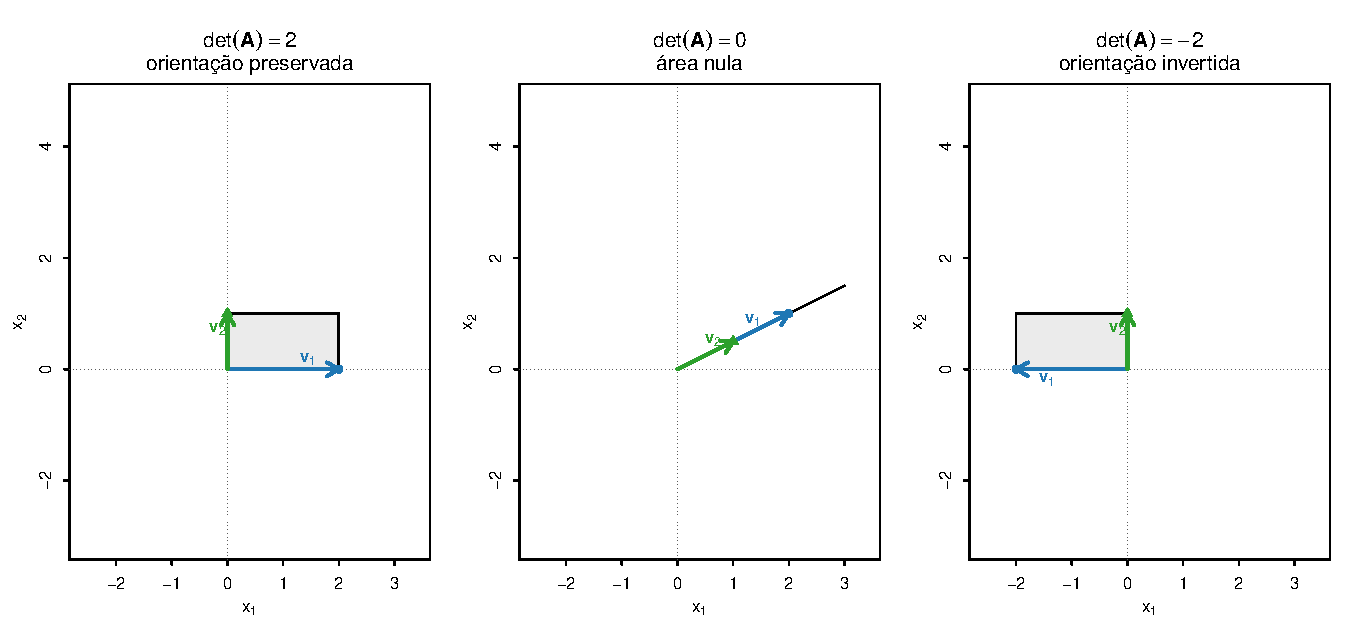
\includegraphics[keepaspectratio]{mod_1_matrizes_files/figure-pdf/fig-interpretacao-determinante-1.pdf}}

}

\caption{\label{fig-interpretacao-determinante}Interpretação geométrica
do determinante em duas dimensões.}

\end{figure}%

Na primeira situação, \(\det(\mathbf{A})=2\): a área é multiplicada por
\(2\) e a orientação é preservada. Na segunda, \(\det(\mathbf{A})=0\): a
região bidimensional é comprimida em uma reta. Na terceira,
\(\det(\mathbf{A})=-2\): a área também é multiplicada por \(2\), mas a
orientação é invertida.

O determinante informa se uma matriz quadrada é invertível. O posto
amplia essa análise para matrizes quadradas ou retangulares.

\subsection{Posto}\label{posto}

O posto mede a dimensão da informação linearmente independente
representada por uma matriz. Ele identifica o número máximo de direções
que não podem ser obtidas como combinações lineares umas das outras.

\begin{definition}[Posto de uma
matriz]\protect\hypertarget{def-posto-matriz}{}\label{def-posto-matriz}

Seja

\[
\mathbf{A}
\in
\mathbb{R}^{n\times p}.
\]

O \textbf{posto} de \(\mathbf{A}\), denotado por

\[
\operatorname{posto}(\mathbf{A}),
\]

é a maior ordem de uma submatriz quadrada de \(\mathbf{A}\) com
determinante diferente de zero.

\end{definition}

Equivalentemente, o posto é:

\begin{itemize}
\tightlist
\item
  o número máximo de colunas linearmente independentes de
  \(\mathbf{A}\);
\item
  o número máximo de linhas linearmente independentes de \(\mathbf{A}\).
\end{itemize}

Esses dois números são sempre iguais. A interpretação do posto por meio
dos espaços gerados pelas linhas e pelas colunas será desenvolvida no
próximo capítulo.

O posto satisfaz

\[
0
\leq
\operatorname{posto}(\mathbf{A})
\leq
\min(n,p).
\]

Uma matriz possui \textbf{posto completo} quando

\[
\operatorname{posto}(\mathbf{A})
=
\min(n,p).
\]

Um caso importante é o produto externo. Se

\[
\mathbf{x}\neq\mathbf{0}
\qquad
\text{e}
\qquad
\mathbf{y}\neq\mathbf{0},
\]

então

\[
\operatorname{posto}
\left(
\mathbf{x}\mathbf{y}^{\top}
\right)
=
1.
\]

De fato, todas as colunas de \(\mathbf{x}\mathbf{y}^{\top}\) são
múltiplos escalares de \(\mathbf{x}\) e, como
\(\mathbf{y}\neq\mathbf{0}\), pelo menos uma dessas colunas é não nula.

Essa estrutura será importante posteriormente nas decomposições
matriciais, em que uma matriz poderá ser representada como soma de
parcelas de posto 1.

Para uma matriz quadrada de ordem \(n\),

\[
\operatorname{posto}(\mathbf{A})=n
\]

equivale à existência de sua inversa.

\begin{theorem}[Condições equivalentes de
invertibilidade]\protect\hypertarget{thm-equivalencias-invertibilidade}{}\label{thm-equivalencias-invertibilidade}

Para

\[
\mathbf{A}
\in
\mathbb{R}^{n\times n},
\]

as afirmações seguintes são equivalentes:

\[
\mathbf{A}
\text{ é invertível},
\]

\[
\det(\mathbf{A})\neq0
\]

e

\[
\operatorname{posto}(\mathbf{A})=n.
\] (Meyer, 2023)

\end{theorem}

\begin{example}[Posto de
matrizes]\protect\hypertarget{exm-posto-matrizes}{}\label{exm-posto-matrizes}

Considere

\[
\mathbf{A}
=
\begin{bmatrix}
1 & 2\\
3 & 4
\end{bmatrix}.
\]

Como

\[
\det(\mathbf{A})
=
1(4)-2(3)
=
-2,
\]

tem-se

\[
\operatorname{posto}(\mathbf{A})
=
2.
\]

Considere agora

\[
\mathbf{B}
=
\begin{bmatrix}
1 & 2\\
2 & 4
\end{bmatrix}.
\]

Como

\[
\det(\mathbf{B})=0
\]

e \(\mathbf{B}\neq\mathbf{0}\),

\[
\operatorname{posto}(\mathbf{B})
=
1.
\]

A segunda linha de \(\mathbf{B}\) é o dobro da primeira, de modo que uma
delas não acrescenta informação linear.

\end{example}

Para uma matriz de dados

\[
\mathbf{X}
\in
\mathbb{R}^{n\times p},
\]

tem-se

\[
\operatorname{posto}(\mathbf{X})
\leq
\min(n,p).
\]

Quando

\[
\operatorname{posto}(\mathbf{X})<p,
\]

existe redundância linear entre as variáveis. A interpretação do posto
em termos de espaços gerados, independência linear e dimensão será
desenvolvida no próximo capítulo.

\subsection{Sistemas lineares}\label{sistemas-lineares}

Um sistema de \(n\) equações lineares com \(p\) incógnitas pode ser
escrito na forma matricial.

\begin{definition}[Sistema
linear]\protect\hypertarget{def-sistema-linear}{}\label{def-sistema-linear}

Sejam

\[
\mathbf{A}
\in
\mathbb{R}^{n\times p},
\qquad
\mathbf{x}
\in
\mathbb{R}^{p}
\]

e

\[
\mathbf{b}
\in
\mathbb{R}^{n}.
\]

O sistema linear associado é

\[
\mathbf{A}\mathbf{x}
=
\mathbf{b}.
\]

A matriz \(\mathbf{A}\) contém os coeficientes, \(\mathbf{x}\) contém as
incógnitas e \(\mathbf{b}\) contém os termos independentes.

\end{definition}

Em componentes, o sistema é

\[
\begin{aligned}
a_{11}x_1+a_{12}x_2+\cdots+a_{1p}x_p &= b_1,\\
a_{21}x_1+a_{22}x_2+\cdots+a_{2p}x_p &= b_2,\\
\vdots \qquad\qquad\qquad\quad & \vdots\\
a_{n1}x_1+a_{n2}x_2+\cdots+a_{np}x_p &= b_n.
\end{aligned}
\]

A matriz aumentada do sistema é

\[
[\mathbf{A}\mid\mathbf{b}]
=
\begin{bmatrix}
a_{11} & \cdots & a_{1p} & b_1\\
\vdots & \ddots & \vdots & \vdots\\
a_{n1} & \cdots & a_{np} & b_n
\end{bmatrix}.
\]

\begin{theorem}[Existência e quantidade de
soluções]\protect\hypertarget{thm-existencia-solucoes-sistema}{}\label{thm-existencia-solucoes-sistema}

Sejam

\[
\mathbf{A}
\in
\mathbb{R}^{n\times p},
\qquad
\mathbf{x}
\in
\mathbb{R}^{p}
\]

e

\[
\mathbf{b}
\in
\mathbb{R}^{n}.
\] O sistema

\[
\mathbf{A}\mathbf{x}
=
\mathbf{b}
\]

possui solução se, e somente se,

\[
\operatorname{posto}(\mathbf{A})
=
\operatorname{posto}
\left(
[\mathbf{A}\mid\mathbf{b}]
\right).
\]

Quando o sistema é consistente:

\begin{itemize}
\tightlist
\item
  a solução é única se
\end{itemize}

\[
\operatorname{posto}(\mathbf{A})=p;
\]

\begin{itemize}
\tightlist
\item
  existem infinitas soluções se
\end{itemize}

\[
\operatorname{posto}(\mathbf{A})<p.
\]

\end{theorem}

\begin{definition}[Sistema linear
homogêneo]\protect\hypertarget{def-sistema-homogeneo}{}\label{def-sistema-homogeneo}

Um \textbf{sistema linear homogêneo} é um sistema da forma

\[
\mathbf A\mathbf x
=
\mathbf 0,
\]

em que

\[
\mathbf A
\in
\mathbb R^{n\times p},
\qquad
\mathbf x
\in
\mathbb R^p
\]

e

\[
\mathbf 0
\in
\mathbb R^n.
\]

Portanto, um sistema homogêneo é um caso particular de sistema linear no
qual todos os termos independentes são iguais a zero.

Todo sistema homogêneo possui pelo menos a \textbf{solução trivial}

\[
\mathbf x
=
\mathbf 0.
\]

Dependendo da matriz \(\mathbf A\), também podem existir
\textbf{soluções não triviais}, isto é, soluções para as quais

\[
\mathbf x
\neq
\mathbf 0.
\]

\end{definition}

A Tabela~\ref{tbl-classificacao-sistemas} resume a classificação das
soluções de um sistema linear.

\begin{longtable}[]{@{}
  >{\raggedright\arraybackslash}p{(\linewidth - 2\tabcolsep) * \real{0.5000}}
  >{\raggedright\arraybackslash}p{(\linewidth - 2\tabcolsep) * \real{0.5000}}@{}}
\caption{Classificação das soluções de um sistema
linear.}\label{tbl-classificacao-sistemas}\tabularnewline
\toprule\noalign{}
\begin{minipage}[b]{\linewidth}\raggedright
Condição
\end{minipage} & \begin{minipage}[b]{\linewidth}\raggedright
Resultado
\end{minipage} \\
\midrule\noalign{}
\endfirsthead
\toprule\noalign{}
\begin{minipage}[b]{\linewidth}\raggedright
Condição
\end{minipage} & \begin{minipage}[b]{\linewidth}\raggedright
Resultado
\end{minipage} \\
\midrule\noalign{}
\endhead
\bottomrule\noalign{}
\endlastfoot
\(\operatorname{posto}(\mathbf{A})\neq\operatorname{posto}([\mathbf{A}\mid\mathbf{b}])\)
& Não existe solução \\
\(\operatorname{posto}(\mathbf{A})=\operatorname{posto}([\mathbf{A}\mid\mathbf{b}])=p\)
& Existe uma única solução \\
\(\operatorname{posto}(\mathbf{A})=\operatorname{posto}([\mathbf{A}\mid\mathbf{b}])<p\)
& Existem infinitas soluções \\
\end{longtable}

\begin{example}[Sistema com solução
única]\protect\hypertarget{exm-sistema-solucao-unica}{}\label{exm-sistema-solucao-unica}

Considere

\[
\begin{aligned}
2x_1+x_2 &= 5,\\
x_1+x_2 &= 3.
\end{aligned}
\]

A forma matricial é

\[
\begin{bmatrix}
2 & 1\\
1 & 1
\end{bmatrix}
\begin{bmatrix}
x_1\\
x_2
\end{bmatrix}
=
\begin{bmatrix}
5\\
3
\end{bmatrix}.
\]

Como

\[
\det
\begin{bmatrix}
2 & 1\\
1 & 1
\end{bmatrix}
=
1,
\]

a matriz de coeficientes é invertível. A solução é

\[
\mathbf{x}
=
\mathbf{A}^{-1}\mathbf{b}
=
\begin{bmatrix}
2\\
1
\end{bmatrix}.
\]

\end{example}

\begin{example}[Sistemas com infinitas soluções e sem
solução]\protect\hypertarget{exm-sistemas-infinitas-sem-solucao}{}\label{exm-sistemas-infinitas-sem-solucao}

Considere inicialmente o sistema

\[
\begin{aligned}
x_1+x_2 &= 2,\\
2x_1+2x_2 &= 4.
\end{aligned}
\]

A segunda equação é o dobro da primeira. Portanto,

\[
\operatorname{posto}(\mathbf{A})
=
\operatorname{posto}
\left(
[\mathbf{A}\mid\mathbf{b}]
\right)
=
1
<
2.
\]

O sistema possui infinitas soluções, que podem ser escritas como

\[
x_1=2-t,
\qquad
x_2=t,
\qquad
t\in\mathbb{R}.
\]

Considere agora

\[
\begin{aligned}
x_1+x_2 &= 2,\\
2x_1+2x_2 &= 5.
\end{aligned}
\]

As linhas da matriz de coeficientes continuam proporcionais, mas os
termos independentes não preservam a mesma proporção. Nesse caso,

\[
\operatorname{posto}(\mathbf{A})
=
1
\]

e

\[
\operatorname{posto}
\left(
[\mathbf{A}\mid\mathbf{b}]
\right)
=
2.
\]

Como os postos são diferentes, o sistema não possui solução.

\end{example}

Para uma matriz quadrada invertível,

\[
\mathbf{A}\mathbf{x}
=
\mathbf{b}
\]

possui a solução única

\[
\mathbf{x}
=
\mathbf{A}^{-1}\mathbf{b}.
\]

\begin{tcolorbox}[enhanced jigsaw, colback=white, breakable, bottomrule=.15mm, left=2mm, arc=.35mm, rightrule=.15mm, colframe=quarto-callout-warning-color-frame, toprule=.15mm, leftrule=.75mm, opacityback=0]

\vspace{-3mm}\textbf{Cálculo da solução}\vspace{3mm}

A expressão

\[
\mathbf{x}
=
\mathbf{A}^{-1}\mathbf{b}
\]

caracteriza a solução quando \(\mathbf{A}\) é invertível. Em cálculos
computacionais, sistemas lineares são resolvidos diretamente, sem
calcular explicitamente a matriz inversa.

\end{tcolorbox}

O número de equações e o número de incógnitas não determinam,
isoladamente, a existência ou a quantidade de soluções:

\begin{itemize}
\tightlist
\item
  se \(n>p\), o sistema é sobredeterminado;
\item
  se \(n<p\), o sistema é subdeterminado;
\item
  se \(n=p\), o sistema é quadrado.
\end{itemize}

A classificação completa depende dos postos de \(\mathbf{A}\) e de
\([\mathbf{A}\mid\mathbf{b}]\).

\subsection{Aprofundamento:
pseudoinversa}\label{aprofundamento-pseudoinversa}

\begin{tcolorbox}[enhanced jigsaw, colback=white, breakable, bottomrule=.15mm, left=2mm, arc=.35mm, rightrule=.15mm, colframe=quarto-callout-note-color-frame, toprule=.15mm, leftrule=.75mm, opacityback=0]

\vspace{-3mm}\textbf{Leitura de aprofundamento}\vspace{3mm}

A pseudoinversa permite estender a resolução de sistemas lineares para
matrizes retangulares ou singulares. Sua construção será desenvolvida no
capítulo sobre decomposição em valores singulares. Nesta seção, são
apresentadas sua definição e suas principais consequências.

\end{tcolorbox}

\begin{definition}[Pseudoinversa de
Moore--Penrose]\protect\hypertarget{def-pseudoinversa-moore-penrose}{}\label{def-pseudoinversa-moore-penrose}

Seja

\[
\mathbf{A}
\in
\mathbb{R}^{n\times p}.
\]

A \textbf{pseudoinversa de Moore--Penrose} de \(\mathbf{A}\) é a única
matriz

\[
\mathbf{A}^{+}
\in
\mathbb{R}^{p\times n}
\]

que satisfaz simultaneamente:

\[
\mathbf{A}\mathbf{A}^{+}\mathbf{A}
=
\mathbf{A},
\]

\[
\mathbf{A}^{+}\mathbf{A}\mathbf{A}^{+}
=
\mathbf{A}^{+},
\]

\[
\left(
\mathbf{A}\mathbf{A}^{+}
\right)^{\top}
=
\mathbf{A}\mathbf{A}^{+}
\]

e

\[
\left(
\mathbf{A}^{+}\mathbf{A}
\right)^{\top}
=
\mathbf{A}^{+}\mathbf{A}.
\]

(Harville, 1997)

\end{definition}

Quando \(\mathbf{A}\) é quadrada e invertível,

\[
\mathbf{A}^{+}
=
\mathbf{A}^{-1}.
\]

Considere o problema

\[
\mathbf{A}\mathbf{x}
=
\mathbf{b}.
\]

O vetor

\[
\mathbf{x}^{+}
=
\mathbf{A}^{+}\mathbf{b}
\]

possui interpretações diferentes conforme a existência e a quantidade de
soluções exatas.

\begin{longtable}[]{@{}
  >{\raggedright\arraybackslash}p{(\linewidth - 2\tabcolsep) * \real{0.5000}}
  >{\raggedright\arraybackslash}p{(\linewidth - 2\tabcolsep) * \real{0.5000}}@{}}
\caption{Interpretação da solução obtida pela
pseudoinversa.}\label{tbl-casos-pseudoinversa}\tabularnewline
\toprule\noalign{}
\begin{minipage}[b]{\linewidth}\raggedright
Situação do sistema
\end{minipage} & \begin{minipage}[b]{\linewidth}\raggedright
Interpretação de \(\mathbf{x}^{+}=\mathbf{A}^{+}\mathbf{b}\)
\end{minipage} \\
\midrule\noalign{}
\endfirsthead
\toprule\noalign{}
\begin{minipage}[b]{\linewidth}\raggedright
Situação do sistema
\end{minipage} & \begin{minipage}[b]{\linewidth}\raggedright
Interpretação de \(\mathbf{x}^{+}=\mathbf{A}^{+}\mathbf{b}\)
\end{minipage} \\
\midrule\noalign{}
\endhead
\bottomrule\noalign{}
\endlastfoot
O sistema é consistente e possui solução única & \(\mathbf{x}^{+}\) é a
solução exata do sistema \\
O sistema é consistente e possui várias soluções & \(\mathbf{x}^{+}\) é
a solução exata de menor norma euclidiana \\
O sistema é inconsistente & \(\mathbf{x}^{+}\) minimiza
\(\|\mathbf{A}\mathbf{x}-\mathbf{b}\|\) e possui a menor norma entre
todos os minimizadores \\
\end{longtable}

No caso inconsistente, \(\mathbf{x}^{+}\) resolve o problema de mínimos
quadrados

\[
\min_{\mathbf{x}\in\mathbb{R}^p}
\|
\mathbf{A}\mathbf{x}
-
\mathbf{b}
\|.
\]

\begin{tcolorbox}[enhanced jigsaw, colback=white, breakable, bottomrule=.15mm, left=2mm, arc=.35mm, rightrule=.15mm, colframe=quarto-callout-caution-color-frame, toprule=.15mm, leftrule=.75mm, opacityback=0]

\vspace{-3mm}\textbf{Pseudoinversa e inversa}\vspace{3mm}

Em geral,

\[
\mathbf{A}^{+}\mathbf{A}
\neq
\mathbf{I}_p
\]

e

\[
\mathbf{A}\mathbf{A}^{+}
\neq
\mathbf{I}_n.
\]

Portanto, a pseudoinversa não satisfaz todas as propriedades da inversa
usual.

\end{tcolorbox}

A construção de \(\mathbf{A}^{+}\), sua interpretação por projeções e
sua relação com o posto serão desenvolvidas no capítulo sobre
decomposição em valores singulares.

\section{Matrizes ortogonais, diagonais e
triangulares}\label{matrizes-ortogonais-diagonais-e-triangulares}

Algumas matrizes quadradas possuem estruturas que simplificam produtos,
inversões e sistemas lineares. Nesta seção são consideradas as matrizes
ortogonais, diagonais e triangulares.

\subsection{Matrizes ortogonais}\label{matrizes-ortogonais}

\begin{definition}[Matriz
ortogonal]\protect\hypertarget{def-matriz-ortogonal}{}\label{def-matriz-ortogonal}

Uma matriz

\[
\mathbf{Q}
\in
\mathbb{R}^{n\times n}
\]

é \textbf{ortogonal} quando

\[
\mathbf{Q}^{\top}\mathbf{Q}
=
\mathbf{I}_n.
\]

\end{definition}

A condição anterior implica que \(\mathbf{Q}\) é invertível e

\[
\mathbf{Q}^{-1}
=
\mathbf{Q}^{\top}.
\]

Consequentemente,

\[
\mathbf{Q}\mathbf{Q}^{\top}
=
\mathbf{I}_n.
\]

Escrevendo as colunas de \(\mathbf{Q}\) como

\[
\mathbf{Q}
=
\left[
\mathbf{q}_{\cdot1}
\;
\mathbf{q}_{\cdot2}
\;
\cdots
\;
\mathbf{q}_{\cdot n}
\right],
\]

tem-se

\[
\mathbf{Q}^{\top}\mathbf{Q}
=
\begin{bmatrix}
\mathbf{q}_{\cdot1}^{\top}\mathbf{q}_{\cdot1} &
\cdots &
\mathbf{q}_{\cdot1}^{\top}\mathbf{q}_{\cdot n}\\
\vdots &
\ddots &
\vdots\\
\mathbf{q}_{\cdot n}^{\top}\mathbf{q}_{\cdot1} &
\cdots &
\mathbf{q}_{\cdot n}^{\top}\mathbf{q}_{\cdot n}
\end{bmatrix}.
\]

Portanto, \(\mathbf{Q}\) é ortogonal quando suas colunas satisfazem

\[
\mathbf{q}_{\cdot i}^{\top}\mathbf{q}_{\cdot j}
=
\begin{cases}
1, & i=j,\\
0, & i\neq j.
\end{cases}
\]

As colunas possuem norma unitária e são ortogonais duas a duas. A mesma
propriedade é satisfeita pelas linhas de \(\mathbf{Q}\).

\begin{example}[Verificação da
ortogonalidade]\protect\hypertarget{exm-matriz-ortogonal}{}\label{exm-matriz-ortogonal}

Considere

\[
\mathbf{Q}
=
\begin{bmatrix}
0 & -1\\
1 & 0
\end{bmatrix}.
\]

Sua transposta é

\[
\mathbf{Q}^{\top}
=
\begin{bmatrix}
0 & 1\\
-1 & 0
\end{bmatrix}.
\]

Calculando o produto,

\[
\mathbf{Q}^{\top}\mathbf{Q}
=
\begin{bmatrix}
0 & 1\\
-1 & 0
\end{bmatrix}
\begin{bmatrix}
0 & -1\\
1 & 0
\end{bmatrix}
=
\mathbf{I}_2.
\]

Logo, \(\mathbf{Q}\) é ortogonal e

\[
\mathbf{Q}^{-1}
=
\mathbf{Q}^{\top}.
\]

\end{example}

\begin{theorem}[Preservação do produto
interno]\protect\hypertarget{thm-preservacao-produto-interno}{}\label{thm-preservacao-produto-interno}

Se \(\mathbf{Q}\in\mathbb{R}^{n\times n}\) é ortogonal, então, para
quaisquer \(\mathbf{x},\mathbf{y}\in\mathbb{R}^n\),

\[
(\mathbf{Q}\mathbf{x})^{\top}
(\mathbf{Q}\mathbf{y})
=
\mathbf{x}^{\top}\mathbf{y}.
\]

\end{theorem}

\begin{proof}
Pela associatividade do produto matricial,

\[
(\mathbf{Q}\mathbf{x})^{\top}
(\mathbf{Q}\mathbf{y})
=
\mathbf{x}^{\top}
\mathbf{Q}^{\top}
\mathbf{Q}
\mathbf{y}.
\]

Como

\[
\mathbf{Q}^{\top}\mathbf{Q}
=
\mathbf{I}_n,
\]

obtém-se

\[
(\mathbf{Q}\mathbf{x})^{\top}
(\mathbf{Q}\mathbf{y})
=
\mathbf{x}^{\top}
\mathbf{I}_n
\mathbf{y}
=
\mathbf{x}^{\top}\mathbf{y}.
\]
\end{proof}

Tomando \(\mathbf{y}=\mathbf{x}\), obtém-se

\[
\|\mathbf{Q}\mathbf{x}\|
=
\|\mathbf{x}\|.
\]

Aplicando a mesma propriedade ao vetor \(\mathbf{x}-\mathbf{y}\),

\[
\|
\mathbf{Q}\mathbf{x}
-
\mathbf{Q}\mathbf{y}
\|
=
\|
\mathbf{x}
-
\mathbf{y}
\|.
\]

Portanto, matrizes ortogonais preservam produtos internos, normas e
distâncias euclidianas.

Além disso,

\[
\det(\mathbf{Q})^2
=
\det(\mathbf{Q}^{\top}\mathbf{Q})
=
\det(\mathbf{I}_n)
=
1,
\]

de modo que

\[
\det(\mathbf{Q})
\in
\{-1,1\}.
\]

O produto de matrizes ortogonais de mesma ordem também é ortogonal.

As interpretações das matrizes ortogonais como rotações, reflexões e
mudanças de orientação serão desenvolvidas no capítulo sobre
transformações lineares.

\subsection{Matrizes diagonais}\label{matrizes-diagonais}

\begin{definition}[Matriz
diagonal]\protect\hypertarget{def-matriz-diagonal}{}\label{def-matriz-diagonal}

Uma matriz

\[
\mathbf{D}
=
(d_{ij})_{n\times n}
\in
\mathbb{R}^{n\times n}
\]

é \textbf{diagonal} quando

\[
d_{ij}=0
\qquad
\text{para}
\qquad
i\neq j.
\]

Uma matriz diagonal possui a forma

\[
\mathbf{D}
=
\begin{bmatrix}
d_1 & 0 & \cdots & 0\\
0 & d_2 & \cdots & 0\\
\vdots & \vdots & \ddots & \vdots\\
0 & 0 & \cdots & d_n
\end{bmatrix}
=
\operatorname{diag}
\left(
\begin{bmatrix}
d_1 \\
d_2\\
\vdots\\
d_n
\end{bmatrix}
\right).
\]

\end{definition}

A matriz identidade é uma matriz diagonal:

\[
\mathbf{I}_n
=
\operatorname{diag}(1,1,\ldots,1).
\]

Toda matriz diagonal é simétrica, pois

\[
\mathbf{D}^{\top}
=
\mathbf{D}.
\]

Para

\[
\mathbf{x}
=
\begin{bmatrix}
x_1\\
x_2\\
\vdots\\
x_n
\end{bmatrix},
\]

o produto por uma matriz diagonal é

\[
\mathbf{D}\mathbf{x}
=
\begin{bmatrix}
d_1x_1\\
d_2x_2\\
\vdots\\
d_nx_n
\end{bmatrix}.
\]

Cada componente de \(\mathbf{x}\) é multiplicada pelo elemento
correspondente da diagonal.

\begin{example}[Produto por uma matriz
diagonal]\protect\hypertarget{exm-produto-matriz-diagonal}{}\label{exm-produto-matriz-diagonal}

Considere

\[
\mathbf{D}
=
\begin{bmatrix}
2 & 0 & 0\\
0 & -1 & 0\\
0 & 0 & 3
\end{bmatrix}
\]

e

\[
\mathbf{x}
=
\begin{bmatrix}
1\\
4\\
-2
\end{bmatrix}.
\]

Então,

\[
\mathbf{D}\mathbf{x}
=
\begin{bmatrix}
2(1)\\
-1(4)\\
3(-2)
\end{bmatrix}
=
\begin{bmatrix}
2\\
-4\\
-6
\end{bmatrix}.
\]

\end{example}

A soma e o produto de matrizes diagonais de mesma ordem também são
diagonais. Se

\[
\mathbf{D}_1
=
\operatorname{diag}(d_1,\ldots,d_n)
\]

e

\[
\mathbf{D}_2
=
\operatorname{diag}(e_1,\ldots,e_n),
\]

então

\[
\mathbf{D}_1+\mathbf{D}_2
=
\operatorname{diag}
(d_1+e_1,\ldots,d_n+e_n)
\]

e

\[
\mathbf{D}_1\mathbf{D}_2
=
\operatorname{diag}
(d_1e_1,\ldots,d_ne_n).
\]

Duas matrizes diagonais de mesma ordem comutam:

\[
\mathbf{D}_1\mathbf{D}_2
=
\mathbf{D}_2\mathbf{D}_1.
\]

O determinante de uma matriz diagonal é o produto dos elementos de sua
diagonal:

\[
\det(\mathbf{D})
=
\prod_{i=1}^{n}d_i.
\]

Logo, \(\mathbf{D}\) é invertível se, e somente se,

\[
d_i\neq0,
\qquad
i=1,\ldots,n.
\]

Nesse caso,

\[
\mathbf{D}^{-1}
=
\operatorname{diag}
\left(
\frac{1}{d_1},
\frac{1}{d_2},
\ldots,
\frac{1}{d_n}
\right).
\]

Para um inteiro positivo \(k\),

\[
\mathbf{D}^k
=
\operatorname{diag}
(d_1^k,d_2^k,\ldots,d_n^k).
\]

As matrizes diagonais serão utilizadas nas decomposições matriciais
estudadas nos capítulos posteriores.

\subsection{Matrizes triangulares}\label{matrizes-triangulares}

\begin{definition}[Matrizes
triangulares]\protect\hypertarget{def-matriz-triangular}{}\label{def-matriz-triangular}

Uma matriz

\[
\mathbf{U}
=
(u_{ij})_{n\times n}
\]

é \textbf{triangular superior} quando

\[
u_{ij}=0
\qquad
\text{para}
\qquad
i>j.
\]

Sua forma geral é

\[
\mathbf{U}
=
\begin{bmatrix}
u_{11} & u_{12} & \cdots & u_{1n}\\
0 & u_{22} & \cdots & u_{2n}\\
\vdots & \ddots & \ddots & \vdots\\
0 & \cdots & 0 & u_{nn}
\end{bmatrix}.
\]

Uma matriz

\[
\mathbf{L}
=
(\ell_{ij})_{n\times n}
\]

é \textbf{triangular inferior} quando

\[
\ell_{ij}=0
\qquad
\text{para}
\qquad
i<j.
\]

Sua forma geral é

\[
\mathbf{L}
=
\begin{bmatrix}
\ell_{11} & 0 & \cdots & 0\\
\ell_{21} & \ell_{22} & \cdots & 0\\
\vdots & \vdots & \ddots & \vdots\\
\ell_{n1} & \ell_{n2} & \cdots & \ell_{nn}
\end{bmatrix}.
\]

\end{definition}

A transposta de uma matriz triangular superior é triangular inferior:

\[
\mathbf{U}^{\top}
\text{ é triangular inferior}.
\]

Da mesma forma,

\[
\mathbf{L}^{\top}
\text{ é triangular superior}.
\]

A soma e o produto de matrizes triangulares superiores de mesma ordem
permanecem triangulares superiores. A mesma propriedade vale para
matrizes triangulares inferiores.

O determinante de uma matriz triangular é o produto dos elementos de sua
diagonal:

\[
\det(\mathbf{U})
=
\prod_{i=1}^{n}u_{ii}
\]

e

\[
\det(\mathbf{L})
=
\prod_{i=1}^{n}\ell_{ii}.
\]

Uma matriz triangular é invertível se, e somente se, todos os elementos
de sua diagonal são diferentes de zero.

\begin{example}[Determinante de uma matriz
triangular]\protect\hypertarget{exm-matriz-triangular}{}\label{exm-matriz-triangular}

Considere

\[
\mathbf{U}
=
\begin{bmatrix}
2 & 1 & -1\\
0 & 3 & 4\\
0 & 0 & 5
\end{bmatrix}.
\]

Como \(\mathbf{U}\) é triangular superior,

\[
\det(\mathbf{U})
=
2(3)(5)
=
30.
\]

Como todos os elementos da diagonal são diferentes de zero,
\(\mathbf{U}\) é invertível.

\end{example}

\subsection{Aprofundamento: sistemas
triangulares}\label{aprofundamento-sistemas-triangulares}

\begin{tcolorbox}[enhanced jigsaw, colback=white, breakable, bottomrule=.15mm, left=2mm, arc=.35mm, rightrule=.15mm, colframe=quarto-callout-note-color-frame, toprule=.15mm, leftrule=.75mm, opacityback=0]

\vspace{-3mm}\textbf{Leitura de aprofundamento}\vspace{3mm}

Os sistemas triangulares mostram como a estrutura de uma matriz pode
simplificar a resolução de equações. Esses procedimentos também aparecem
nas decomposições matriciais estudadas posteriormente.

\end{tcolorbox}

Um sistema cuja matriz de coeficientes é triangular pode ser resolvido
sequencialmente.

Para uma matriz triangular superior,

\[
\mathbf{U}\mathbf{x}
=
\mathbf{b},
\]

a última equação contém somente a incógnita \(x_n\). Após determinar
\(x_n\), substitui-se seu valor na equação anterior. Esse procedimento
continua até a determinação de \(x_1\) e é denominado
\textbf{substituição regressiva}.

\begin{example}[Sistema triangular
superior]\protect\hypertarget{exm-substituicao-regressiva}{}\label{exm-substituicao-regressiva}

Considere o sistema

\[
\begin{aligned}
x_1+2x_2-x_3 &= 4,\\
2x_2+3x_3 &= 7,\\
x_3 &= 1.
\end{aligned}
\]

Sua forma matricial é

\[
\begin{bmatrix}
1 & 2 & -1\\
0 & 2 & 3\\
0 & 0 & 1
\end{bmatrix}
\begin{bmatrix}
x_1\\
x_2\\
x_3
\end{bmatrix}
=
\begin{bmatrix}
4\\
7\\
1
\end{bmatrix}.
\]

A última equação fornece

\[
x_3=1.
\]

Substituindo na segunda equação,

\[
2x_2+3(1)=7,
\]

de modo que

\[
x_2=2.
\]

Substituindo os valores obtidos na primeira equação,

\[
x_1+2(2)-1=4,
\]

resulta

\[
x_1=1.
\]

Portanto,

\[
\mathbf{x}
=
\begin{bmatrix}
1\\
2\\
1
\end{bmatrix}.
\]

\end{example}

Para um sistema

\[
\mathbf{L}\mathbf{x}
=
\mathbf{b},
\]

com \(\mathbf{L}\) triangular inferior, a resolução começa pela primeira
equação e segue até a última. Esse procedimento é denominado
\textbf{substituição progressiva}.

As matrizes triangulares aparecem na resolução de sistemas e em
decomposições matriciais. As formas bilineares e quadráticas serão
estudadas na próxima seção.

\section{Formas bilineares, formas quadráticas e
positividade}\label{formas-bilineares-formas-quadruxe1ticas-e-positividade}

As formas bilineares associam dois vetores a um escalar e são lineares
em cada argumento separadamente. Quando uma forma bilinear é avaliada
utilizando o mesmo vetor em seus dois argumentos, obtém-se uma função de
um único vetor, denominada forma quadrática.

Essa relação permite conectar propriedades das matrizes, como simetria e
positividade, a expressões escalares que aparecem frequentemente na
análise multivariada, entre elas produtos internos, normas, variâncias e
distâncias.

\subsection{Formas bilineares}\label{formas-bilineares}

\begin{definition}[Forma
bilinear]\protect\hypertarget{def-forma-bilinear}{}\label{def-forma-bilinear}

Uma função

\[
g:
\mathbb R^p
\times
\mathbb R^p
\longrightarrow
\mathbb R
\]

é denominada \textbf{forma bilinear} quando é linear separadamente em
cada argumento.

Isso significa que, para quaisquer

\[
\mathbf{x},
\mathbf{y},
\mathbf{z}
\in
\mathbb R^p
\]

e quaisquer

\[
\beta\in\mathbb R,
\]

tem-se

\[
g
\left(
\mathbf{x}+\beta\mathbf{z},
\mathbf{y}
\right)
=
g
\left(
\mathbf{x},\mathbf{y}
\right)
+
\beta
g
\left(
\mathbf{z},\mathbf{y}
\right)
\]

e

\[
g
\left(
\mathbf{x},
\mathbf{z}+\beta\mathbf{y}
\right)
=
g
\left(
\mathbf{x},\mathbf{z}
\right)
+
\beta
g
\left(
\mathbf{x},\mathbf{y}
\right).
\]

\end{definition}

A bilinearidade significa, portanto, que, mantendo um dos argumentos
fixo, a forma bilinear é uma função linear do outro argumento.

Fixado \(\mathbf{y}\in\mathbb R^p\), a função

\[
\mathbf{x}
\longmapsto
g
\left(
\mathbf{x},\mathbf{y}
\right)
\]

é linear em \(\mathbf{x}\). Analogamente, fixado
\(\mathbf{x}\in\mathbb R^p\), a função

\[
\mathbf{y}
\longmapsto
g
\left(
\mathbf{x},\mathbf{y}
\right)
\]

é linear em \(\mathbf{y}\).

Um caso particulamente importante para a estatística são as formas
bilineares simétricas.

\begin{definition}[Forma bilinear
simétrica]\protect\hypertarget{def-forma-bilinear-simetrica}{}\label{def-forma-bilinear-simetrica}

Uma forma bilinear

\[
g:
\mathbb R^p
\times
\mathbb R^p
\longrightarrow
\mathbb R
\]

é denominada \textbf{simétrica} quando

\[
g
\left(
\mathbf{x},\mathbf{y}
\right)
=
g
\left(
\mathbf{y},\mathbf{x}
\right)
\]

para quaisquer

\[
\mathbf{x},\mathbf{y}\in\mathbb R^p.
\]

\end{definition}

\begin{example}[Produto interno como forma bilinear
simétrica]\protect\hypertarget{exm-produto-interno-forma-bilinear}{}\label{exm-produto-interno-forma-bilinear}

O produto interno usual em \(\mathbb R^p\),

\[
g
\left(
\mathbf{x},\mathbf{y}
\right)
=
\langle
\mathbf{x},\mathbf{y}
\rangle,
\]

é um exemplo de forma bilinear simétrica, pois,

\[
\langle
\mathbf{x},\mathbf{y}
\rangle
=
\langle
\mathbf{y},\mathbf{x}
\rangle,
\]

ou, equivalentemente,

\[
\mathbf{x}^{\top}\mathbf y
=
\mathbf{y}^{\top}\mathbf x.
\]

\end{example}

Nem toda forma bilinear é simétrica.

\begin{example}[Bilinearidade e ausência de
simetria]\protect\hypertarget{exm-forma-bilinear}{}\label{exm-forma-bilinear}

Considere a matriz

\[
\mathbf A
=
\begin{bmatrix}
2 & 1\\
-1 & 3
\end{bmatrix}
\]

e os vetores

\[
\mathbf{x}
=
\begin{bmatrix}
x_1\\
x_2
\end{bmatrix},
\qquad
\mathbf{y}
=
\begin{bmatrix}
y_1\\
y_2
\end{bmatrix}.
\]

A função

\[
g
\left(
\mathbf{x},\mathbf{y}
\right)
=
\mathbf{x}^{\top}
\mathbf A
\mathbf y
\]

é dada por

\[
\begin{aligned}
g
\left(
\mathbf{x},\mathbf{y}
\right)
&=
\begin{bmatrix}
x_1 & x_2
\end{bmatrix}
\begin{bmatrix}
2 & 1\\
-1 & 3
\end{bmatrix}
\begin{bmatrix}
y_1\\
y_2
\end{bmatrix}\\
&=
\begin{bmatrix}
x_1 & x_2
\end{bmatrix}
\begin{bmatrix}
2y_1+y_2\\
-y_1+3y_2
\end{bmatrix}\\
&=
2x_1y_1
+
x_1y_2
-
x_2y_1
+
3x_2y_2.
\end{aligned}
\]

Para verificar a linearidade no primeiro argumento, sejam
\(\mathbf{x}_1,\mathbf{x}_2,\mathbf{y}\in\mathbb R^2\) e
\(\beta\in\mathbb R\). Então,

\[
\begin{aligned}
g
\left(
\mathbf{x}_1+\beta\mathbf{x}_2,
\mathbf{y}
\right)
&=
\left(
\mathbf{x}_1+\beta\mathbf{x}_2
\right)^{\top}
\mathbf A
\mathbf y\\
&=
\mathbf{x}_1^{\top}
\mathbf A
\mathbf y
+
\beta
\mathbf{x}_2^{\top}
\mathbf A
\mathbf y\\
&=
g
\left(
\mathbf{x}_1,\mathbf{y}
\right)
+
\beta
g
\left(
\mathbf{x}_2,\mathbf{y}
\right).
\end{aligned}
\]

Analogamente, para
\(\mathbf{x},\mathbf{y}_1,\mathbf{y}_2\in\mathbb R^2\),

\[
\begin{aligned}
g
\left(
\mathbf{x},
\mathbf{y}_1+\beta\mathbf{y}_2
\right)
&=
\mathbf{x}^{\top}
\mathbf A
\left(
\mathbf{y}_1+\beta\mathbf{y}_2
\right)\\
&=
\mathbf{x}^{\top}
\mathbf A
\mathbf{y}_1
+
\beta
\mathbf{x}^{\top}
\mathbf A
\mathbf{y}_2\\
&=
g
\left(
\mathbf{x},\mathbf{y}_1
\right)
+
\beta
g
\left(
\mathbf{x},\mathbf{y}_2
\right).
\end{aligned}
\]

Portanto, \(g\) é linear em cada argumento separadamente e, assim, é uma
forma bilinear.

Para verificar se a forma bilinear é simétrica, invertem-se os dois
argumentos. Tem-se

\[
\begin{aligned}
g
\left(
\mathbf{y},\mathbf{x}
\right)
&=
2x_1y_1
-
x_1y_2
+
x_2y_1
+
3x_2y_2.
\end{aligned}
\]

Por outro lado,

\[
g
\left(
\mathbf{x},\mathbf{y}
\right)
=
2x_1y_1
+
x_1y_2
-
x_2y_1
+
3x_2y_2.
\]

As duas expressões diferem nos termos cruzados. Portanto, em geral,

\[
g
\left(
\mathbf{x},\mathbf{y}
\right)
\neq
g
\left(
\mathbf{y},\mathbf{x}
\right),
\]

e a forma bilinear não é simétrica.

\end{example}

De modo geral, uma forma bilinear

\[
g
\left(
\mathbf{x},\mathbf{y}
\right)
=
\mathbf{x}^{\top}
\mathbf A
\mathbf y
\]

é simétrica se, e somente se, sua matriz representante é simétrica, isto
é, \(\mathbf A = \mathbf A^{\top}.\)

Uma forma bilinear também pode ser avaliada utilizando o mesmo vetor em
seus dois argumentos. Assim, em vez de considerar

\[
g
\left(
\mathbf{x},\mathbf{y}
\right),
\]

podemos considerar

\[
g
\left(
\mathbf{x},\mathbf{x}
\right).
\]

Essa avaliação produz uma função de um único vetor e conduz às formas
quadráticas.

\subsection{Formas quadráticas}\label{formas-quadruxe1ticas}

\begin{definition}[Forma
quadrática]\protect\hypertarget{def-forma-quadratica}{}\label{def-forma-quadratica}

Seja

\[
g:
\mathbb R^p
\times
\mathbb R^p
\longrightarrow
\mathbb R
\]

uma forma bilinear. A função

\[
Q:
\mathbb R^p
\longrightarrow
\mathbb R
\]

definida por

\[
Q
\left(
\mathbf{x}
\right)
=
g
\left(
\mathbf{x},\mathbf{x}
\right)
\]

é denominada \textbf{forma quadrática} associada a \(g\).

Se a forma bilinear possui representação matricial

\[
g
\left(
\mathbf{x},\mathbf{y}
\right)
=
\mathbf{x}^{\top}
\mathbf A
\mathbf y,
\]

então

\[
Q
\left(
\mathbf{x}
\right)
=
\mathbf{x}^{\top}
\mathbf A
\mathbf{x},
\qquad
\mathbf{x}\in\mathbb R^p.
\]

\end{definition}

A forma bilinear depende de dois argumentos e é linear em cada um deles
separadamente. A forma quadrática, por sua vez, depende de um único
argumento e, em geral, não é uma função linear desse vetor.

De fato, para qualquer \(\alpha\in\mathbb R\),

\[
\begin{aligned}
Q
\left(
\alpha\mathbf{x}
\right)
&=
g
\left(
\alpha\mathbf{x},
\alpha\mathbf{x}
\right)\\
&=
\alpha^2
g
\left(
\mathbf{x},\mathbf{x}
\right)\\
&=
\alpha^2
Q
\left(
\mathbf{x}
\right).
\end{aligned}
\]

Assim,

\[
Q
\left(
\alpha\mathbf{x}
\right)
=
\alpha^2
Q
\left(
\mathbf{x}
\right).
\]

A expressão quadrática pode ser interpretada como a avaliação da forma
bilinear sobre a diagonal do produto cartesiano,

\[
\left\{
(\mathbf{x},\mathbf{x})
:
\mathbf{x}\in\mathbb R^p
\right\}
\subset
\mathbb R^p\times\mathbb R^p.
\]

O produto interno fornece um exemplo imediato dessa construção.

\begin{example}[Produto interno e norma ao
quadrado]\protect\hypertarget{exm-produto-interno-forma-quadratica}{}\label{exm-produto-interno-forma-quadratica}

Considere a forma bilinear dada pelo produto interno usual,

\[
g
\left(
\mathbf{x},\mathbf{y}
\right)
=
\langle
\mathbf{x},\mathbf{y}
\rangle.
\]

Ao utilizar o mesmo vetor nos dois argumentos,

\[
Q
\left(
\mathbf{x}
\right)
=
g
\left(
\mathbf{x},\mathbf{x}
\right)
=
\langle
\mathbf{x},\mathbf{x}
\rangle.
\]

Pela definição da norma euclidiana,

\[
\langle
\mathbf{x},\mathbf{x}
\rangle
=
\|\mathbf{x}\|^2.
\]

Portanto,

\[
Q
\left(
\mathbf{x}
\right)
=
\|\mathbf{x}\|^2
=
\mathbf{x}^{\top}\mathbf{x}.
\]

A matriz representante dessa forma quadrática é

\[
\mathbf I_p.
\]

\end{example}

Em geral, se

\[
\mathbf A
=
(a_{ij})_{p\times p},
\]

então

\begin{equation}\phantomsection\label{eq-forma-quadratica-componentes}{
Q
\left(
\mathbf{x}
\right)
=
\mathbf{x}^{\top}
\mathbf A
\mathbf{x}
=
\sum_{i=1}^{p}
\sum_{j=1}^{p}
a_{ij}x_i x_j.
}\end{equation}

Para

\[
\mathbf A
=
\begin{bmatrix}
a & b\\
c & d
\end{bmatrix}
\]

e

\[
\mathbf{x}
=
\begin{bmatrix}
x_1\\
x_2
\end{bmatrix},
\]

tem-se

\[
\begin{aligned}
Q
\left(
\mathbf{x}
\right)
&=
\mathbf{x}^{\top}
\mathbf A
\mathbf{x}\\
&=
\begin{bmatrix}
x_1 & x_2
\end{bmatrix}
\begin{bmatrix}
a & b\\
c & d
\end{bmatrix}
\begin{bmatrix}
x_1\\
x_2
\end{bmatrix}\\
&=
ax_1^2
+
(b+c)x_1x_2
+
dx_2^2.
\end{aligned}
\]

Esse desenvolvimento mostra uma diferença importante entre formas
bilineares e formas quadráticas.

Na forma bilinear

\[
g
\left(
\mathbf{x},\mathbf{y}
\right)
=
\mathbf{x}^{\top}
\mathbf A
\mathbf y,
\]

os elementos \(a_{ij}\) e \(a_{ji}\) podem produzir contribuições
distintas porque os dois vetores não precisam ser iguais.

Na forma quadrática

\[
Q
\left(
\mathbf{x}
\right)
=
\mathbf{x}^{\top}
\mathbf A
\mathbf{x},
\]

os termos fora da diagonal aparecem combinados. No caso bidimensional,
por exemplo, \(b\) e \(c\) aparecem somente por meio da soma

\[
b+c.
\]

Consequentemente, a matriz que aparece em uma representação

\[
Q
\left(
\mathbf{x}
\right)
=
\mathbf{x}^{\top}
\mathbf A
\mathbf{x}
\]

não é necessariamente única quando matrizes não simétricas são
admitidas. Matrizes que diferem apenas por uma parcela antissimétrica
produzem a mesma forma quadrática.

Entretanto, toda forma quadrática possui uma única matriz simétrica que
a representa. Essa propriedade é apresentada na proposição seguinte.

\begin{proposition}[Parte simétrica de uma forma
quadrática]\protect\hypertarget{prp-parte-simetrica-forma-quadratica}{}\label{prp-parte-simetrica-forma-quadratica}

Seja

\[
\mathbf A
\in
\mathbb R^{p\times p}
\]

e defina

\[
\mathbf S
=
\frac{
\mathbf A+\mathbf A^{\top}
}{2}.
\]

Então \(\mathbf S\) é simétrica e, para todo

\[
\mathbf{x}\in\mathbb R^p,
\]

tem-se

\[
\mathbf{x}^{\top}
\mathbf A
\mathbf{x}
=
\mathbf{x}^{\top}
\mathbf S
\mathbf{x}.
\]

Além disso, \(\mathbf S\) é a única matriz simétrica que representa essa
forma quadrática.

\end{proposition}

\begin{proof}
A matriz \(\mathbf A\) pode ser escrita como

\[
\mathbf A
=
\mathbf S+\mathbf K,
\]

em que

\[
\mathbf S
=
\frac{
\mathbf A+\mathbf A^{\top}
}{2}
\]

é simétrica e

\[
\mathbf K
=
\frac{
\mathbf A-\mathbf A^{\top}
}{2}
\]

é antissimétrica.

De fato,

\[
\mathbf S^{\top}
=
\mathbf S
\]

e

\[
\mathbf K^{\top}
=
-\mathbf K.
\]

Assim,

\[
\begin{aligned}
\mathbf{x}^{\top}
\mathbf A
\mathbf{x}
&=
\mathbf{x}^{\top}
\left(
\mathbf S+\mathbf K
\right)
\mathbf{x}\\
&=
\mathbf{x}^{\top}
\mathbf S
\mathbf{x}
+
\mathbf{x}^{\top}
\mathbf K
\mathbf{x}.
\end{aligned}
\]

O termo

\[
\mathbf{x}^{\top}
\mathbf K
\mathbf{x}
\]

é um escalar. Portanto,

\[
\mathbf{x}^{\top}
\mathbf K
\mathbf{x}
=
\left(
\mathbf{x}^{\top}
\mathbf K
\mathbf{x}
\right)^{\top}.
\]

Utilizando a transposição do produto,

\[
\begin{aligned}
\mathbf{x}^{\top}
\mathbf K
\mathbf{x}
&=
\mathbf{x}^{\top}
\mathbf K^{\top}
\mathbf{x}\\
&=
-
\mathbf{x}^{\top}
\mathbf K
\mathbf{x}.
\end{aligned}
\]

Logo,

\[
2
\mathbf{x}^{\top}
\mathbf K
\mathbf{x}
=
0
\]

e, consequentemente,

\[
\mathbf{x}^{\top}
\mathbf K
\mathbf{x}
=
0.
\]

Portanto,

\[
\mathbf{x}^{\top}
\mathbf A
\mathbf{x}
=
\mathbf{x}^{\top}
\mathbf S
\mathbf{x}.
\]

Resta mostrar a unicidade da representação simétrica.

Suponha que \(\mathbf S_1\) e \(\mathbf S_2\) sejam duas matrizes
simétricas que representem a mesma forma quadrática. Então,

\[
\mathbf{x}^{\top}
\mathbf S_1
\mathbf{x}
=
\mathbf{x}^{\top}
\mathbf S_2
\mathbf{x}
\]

para todo \(\mathbf{x}\in\mathbb R^p\).

Definindo

\[
\mathbf D
=
\mathbf S_1-\mathbf S_2,
\]

a matriz \(\mathbf D\) também é simétrica e satisfaz

\[
\mathbf{x}^{\top}
\mathbf D
\mathbf{x}
=
0
\]

para todo \(\mathbf{x}\in\mathbb R^p\).

Para quaisquer \(\mathbf{x},\mathbf{y}\in\mathbb R^p\),

\[
\begin{aligned}
0
&=
(\mathbf{x}+\mathbf{y})^{\top}
\mathbf D
(\mathbf{x}+\mathbf{y})\\
&=
\mathbf{x}^{\top}
\mathbf D
\mathbf{x}
+
\mathbf{x}^{\top}
\mathbf D
\mathbf{y}
+
\mathbf{y}^{\top}
\mathbf D
\mathbf{x}
+
\mathbf{y}^{\top}
\mathbf D
\mathbf{y}.
\end{aligned}
\]

Como \(\mathbf D\) é simétrica,

\[
\mathbf{y}^{\top}
\mathbf D
\mathbf{x}
=
\mathbf{x}^{\top}
\mathbf D
\mathbf{y},
\]

e os termos quadráticos são nulos. Assim,

\[
2
\mathbf{x}^{\top}
\mathbf D
\mathbf{y}
=
0
\]

para quaisquer \(\mathbf{x},\mathbf{y}\in\mathbb R^p\).

Logo,

\[
\mathbf{x}^{\top}
\mathbf D
\mathbf{y}
=
0
\]

para quaisquer \(\mathbf{x},\mathbf{y}\in\mathbb R^p\).

Em particular, tomando os vetores da base canônica,

\[
\mathbf{x}
=
\mathbf e_i
\qquad
\text{e}
\qquad
\mathbf{y}
=
\mathbf e_j,
\]

obtém-se

\[
\mathbf e_i^{\top}
\mathbf D
\mathbf e_j
=
d_{ij}
=
0
\]

para todos \(i\) e \(j\).

Portanto,

\[
\mathbf D
=
\mathbf 0,
\]

o que implica

\[
\mathbf S_1
=
\mathbf S_2.
\]
\end{proof}

Assim, embora uma forma quadrática possa possuir diferentes
representações por matrizes não simétricas, sua representação por uma
matriz simétrica é única.

Por essa razão, no estudo de formas quadráticas, pode-se trabalhar sem
perda de generalidade com matrizes simétricas.

Observe que essa propriedade é específica das formas quadráticas. Para
uma forma bilinear geral,

\[
g
\left(
\mathbf{x},\mathbf{y}
\right)
=
\mathbf{x}^{\top}
\mathbf A
\mathbf y,
\]

a parte antissimétrica de \(\mathbf A\) pode contribuir para o valor da
expressão quando

\[
\mathbf{x}\neq\mathbf y.
\]

Quando os dois argumentos coincidem, essa contribuição desaparece.

\begin{example}[Expansão de uma forma
quadrática]\protect\hypertarget{exm-forma-quadratica}{}\label{exm-forma-quadratica}

Considere

\[
\mathbf A
=
\begin{bmatrix}
2 & 1\\
1 & 3
\end{bmatrix}
\]

e

\[
\mathbf{x}
=
\begin{bmatrix}
x_1\\
x_2
\end{bmatrix}.
\]

A forma quadrática associada a \(\mathbf A\) é

\[
Q
\left(
\mathbf{x}
\right)
=
\mathbf{x}^{\top}
\mathbf A
\mathbf{x}.
\]

Então,

\[
\begin{aligned}
Q
\left(
\mathbf{x}
\right)
&=
\begin{bmatrix}
x_1 & x_2
\end{bmatrix}
\begin{bmatrix}
2 & 1\\
1 & 3
\end{bmatrix}
\begin{bmatrix}
x_1\\
x_2
\end{bmatrix}.
\end{aligned}
\]

Efetuando os produtos,

\[
Q
\left(
\mathbf{x}
\right)
=
2x_1^2
+
2x_1x_2
+
3x_2^2.
\]

Para

\[
\mathbf{x}
=
\begin{bmatrix}
1\\
2
\end{bmatrix},
\]

obtém-se

\[
\begin{aligned}
Q
\left(
\mathbf{x}
\right)
&=
2(1)^2
+
2(1)(2)
+
3(2)^2\\
&=
2+4+12\\
&=
18.
\end{aligned}
\]

\end{example}

\subsection{Positividade}\label{positividade}

Como toda forma quadrática pode ser representada por uma única matriz
simétrica, propriedades importantes da forma quadrática podem ser
estudadas a partir dos valores assumidos por

\[
Q
\left(
\mathbf{x}
\right)
=
\mathbf{x}^{\top}
\mathbf A
\mathbf{x},
\]

com \(\mathbf A\) simétrica.

A classificação em positiva definida, semidefinida positiva, negativa
definida, semidefinida negativa ou indefinida depende do sinal assumido
por essa expressão.

\begin{definition}[Classificação de matrizes simétricas pela forma
quadrática]\protect\hypertarget{def-classificacao-positividade}{}\label{def-classificacao-positividade}

Seja

\[
\mathbf A
\in
\mathbb R^{p\times p}
\]

uma matriz simétrica e considere a forma quadrática

\[
q_{\mathbf A}(\mathbf x)
=
\mathbf x^{\top}
\mathbf A
\mathbf x.
\]

A matriz \(\mathbf A\) é:

\begin{itemize}
\item
  \textbf{positiva definida} quando

  \[
  \mathbf x^{\top}
  \mathbf A
  \mathbf x
  >
  0
  \]

  para todo \(\mathbf x\neq\mathbf0\). Nesse caso, escreve-se

  \[
  \mathbf A\succ\mathbf0;
  \]
\item
  \textbf{semidefinida positiva} quando

  \[
  \mathbf x^{\top}
  \mathbf A
  \mathbf x
  \geq
  0
  \]

  para todo \(\mathbf x\in\mathbb R^p\). Nesse caso, escreve-se

  \[
  \mathbf A\succeq\mathbf0;
  \]
\item
  \textbf{negativa definida} quando

  \[
  \mathbf x^{\top}
  \mathbf A
  \mathbf x
  <
  0
  \]

  para todo \(\mathbf x\neq\mathbf0\). Nesse caso, escreve-se

  \[
  \mathbf A\prec\mathbf0;
  \]
\item
  \textbf{semidefinida negativa} quando

  \[
  \mathbf x^{\top}
  \mathbf A
  \mathbf x
  \leq
  0
  \]

  para todo \(\mathbf x\in\mathbb R^p\). Nesse caso, escreve-se

  \[
  \mathbf A\preceq\mathbf0;
  \]
\item
  \textbf{indefinida} quando existem vetores não nulos
  \(\mathbf x,\mathbf y\in\mathbb R^p\) tais que

  \[
  \mathbf x^{\top}
  \mathbf A
  \mathbf x
  >
  0
  \]

  e

  \[
  \mathbf y^{\top}
  \mathbf A
  \mathbf y
  <
  0.
  \]

  Para matrizes indefinidas, não se utiliza uma relação de ordem do tipo
  \(\mathbf A\succeq\mathbf0\) ou \(\mathbf A\preceq\mathbf0\).
\end{itemize}

\end{definition}

As notações \(\succ\), \(\succeq\), \(\prec\) e \(\preceq\) expressam a
ordem de Löwner para matrizes simétricas. Em particular,

\[
\begin{aligned}
\mathbf A\succ\mathbf0
&\quad\Longleftrightarrow\quad
\mathbf A \text{ é positiva definida},\\
\mathbf A\succeq\mathbf0
&\quad\Longleftrightarrow\quad
\mathbf A \text{ é semidefinida positiva},\\
\mathbf A\prec\mathbf0
&\quad\Longleftrightarrow\quad
\mathbf A \text{ é negativa definida},\\
\mathbf A\preceq\mathbf0
&\quad\Longleftrightarrow\quad
\mathbf A \text{ é semidefinida negativa}.
\end{aligned}
\]

produto interno usual fornece um exemplo imediato de forma quadrática
associada a uma matriz positiva definida.

Como

\[
Q
\left(
\mathbf{x}
\right)
=
\mathbf{x}^{\top}
\mathbf I_p
\mathbf{x}
=
\|\mathbf{x}\|^2,
\]

tem-se

\[
Q
\left(
\mathbf{x}
\right)
>
0
\]

para todo

\[
\mathbf{x}\neq\mathbf 0.
\]

Portanto, a matriz identidade

\[
\mathbf I_p
\]

é positiva definida.

Outro exemplo importante de matriz semidefinida positiva é obtido pelo
produto externo de um vetor consigo mesmo.

Para

\[
\mathbf{x},\mathbf{z}\in\mathbb R^p,
\]

considere

\[
\mathbf{x}\mathbf{x}^{\top}.
\]

Então,

\[
\begin{aligned}
\mathbf{z}^{\top}
\left(
\mathbf{x}\mathbf{x}^{\top}
\right)
\mathbf{z}
&=
\left(
\mathbf{z}^{\top}\mathbf{x}
\right)
\left(
\mathbf{x}^{\top}\mathbf{z}
\right)\\
&=
\left(
\mathbf{x}^{\top}\mathbf{z}
\right)^2\\
&\geq
0.
\end{aligned}
\]

Portanto,

\[
\mathbf{x}\mathbf{x}^{\top}
\]

é semidefinida positiva.

Se \(\mathbf{x}\neq\mathbf 0\), então

\[
\operatorname{rank}
\left(
\mathbf{x}\mathbf{x}^{\top}
\right)
=
1.
\]

Assim, quando \(p>1\), existem vetores não nulos \(\mathbf z\)
ortogonais a \(\mathbf x\). Para esses vetores,

\[
\mathbf{x}^{\top}\mathbf z
=
0
\]

e, portanto,

\[
\mathbf{z}^{\top}
\left(
\mathbf{x}\mathbf{x}^{\top}
\right)
\mathbf{z}
=
0.
\]

Logo, para \(p>1\) e \(\mathbf{x}\neq\mathbf 0\), a matriz

\[
\mathbf{x}\mathbf{x}^{\top}
\]

é semidefinida positiva, mas não positiva definida.

Esse tipo de matriz terá importância particular na construção das
matrizes de covariâncias, que envolvem somas de produtos externos de
vetores de desvios.

\begin{example}[Classificação de formas
quadráticas]\protect\hypertarget{exm-positividade-matrizes}{}\label{exm-positividade-matrizes}

Considere inicialmente

\[
\mathbf A
=
\begin{bmatrix}
2 & 0\\
0 & 3
\end{bmatrix}.
\]

Para

\[
\mathbf{x}
=
\begin{bmatrix}
x_1\\
x_2
\end{bmatrix},
\]

tem-se

\[
Q
\left(
\mathbf{x}
\right)
=
\mathbf{x}^{\top}
\mathbf A
\mathbf{x}
=
2x_1^2+3x_2^2.
\]

Como

\[
2x_1^2+3x_2^2
>
0
\]

para todo

\[
\mathbf{x}\neq\mathbf 0,
\]

a matriz \(\mathbf A\) é positiva definida.

Considere agora

\[
\mathbf B
=
\begin{bmatrix}
1 & 0\\
0 & 0
\end{bmatrix}.
\]

Nesse caso,

\[
Q
\left(
\mathbf{x}
\right)
=
\mathbf{x}^{\top}
\mathbf B
\mathbf{x}
=
x_1^2
\geq
0.
\]

Portanto, \(\mathbf B\) é semidefinida positiva.

Entretanto, para vetores não nulos da forma

\[
\mathbf{x}
=
\begin{bmatrix}
0\\
x_2
\end{bmatrix},
\qquad
x_2\neq0,
\]

tem-se

\[
Q
\left(
\mathbf{x}
\right)
=
0.
\]

Assim, \(\mathbf B\) não é positiva definida.

Finalmente, considere

\[
\mathbf C
=
\begin{bmatrix}
1 & 0\\
0 & -1
\end{bmatrix}.
\]

A forma quadrática associada é

\[
Q
\left(
\mathbf{x}
\right)
=
\mathbf{x}^{\top}
\mathbf C
\mathbf{x}
=
x_1^2-x_2^2.
\]

Para

\[
\mathbf{x}
=
\begin{bmatrix}
1\\
0
\end{bmatrix},
\]

obtém-se

\[
Q
\left(
\mathbf{x}
\right)
=
1>0.
\]

Por outro lado, para

\[
\mathbf{y}
=
\begin{bmatrix}
0\\
1
\end{bmatrix},
\]

obtém-se

\[
Q
\left(
\mathbf{y}
\right)
=
-1<0.
\]

Portanto, a forma quadrática assume valores positivos e negativos, e a
matriz \(\mathbf C\) é indefinida.

\end{example}

\subsection{Superfícies de nível}\label{superfuxedcies-de-nuxedvel}

Uma superfície de nível de uma forma quadrática é definida por

\[
\mathbf{x}^{\top}\mathbf{A}\mathbf{x}
=
c,
\]

em que \(c\) é uma constante.

Quando \(\mathbf{A}\) é positiva definida e \(c>0\), as superfícies de
nível são elipsoides. Em duas dimensões, correspondem a elipses. Para
\(c=0\), a superfície contém somente o vetor nulo, enquanto, para
\(c<0\), não existem pontos que satisfaçam a equação.

Quando \(\mathbf{A}\) é indefinida, a forma quadrática assume valores
positivos e negativos. Em duas dimensões, no caso indefinido não
singular, os níveis não nulos formam hipérboles. O nível zero pode
formar um par de retas que se cruzam na origem. Por exemplo,

\[
x_1^2-x_2^2=0
\]

equivale a

\[
x_2=x_1
\qquad
\text{ou}
\qquad
x_2=-x_1.
\]

A Figura~\ref{fig-formas-quadraticas} apresenta três formas quadráticas
em \(\mathbb{R}^2\).

\begin{figure}

\centering{

\pandocbounded{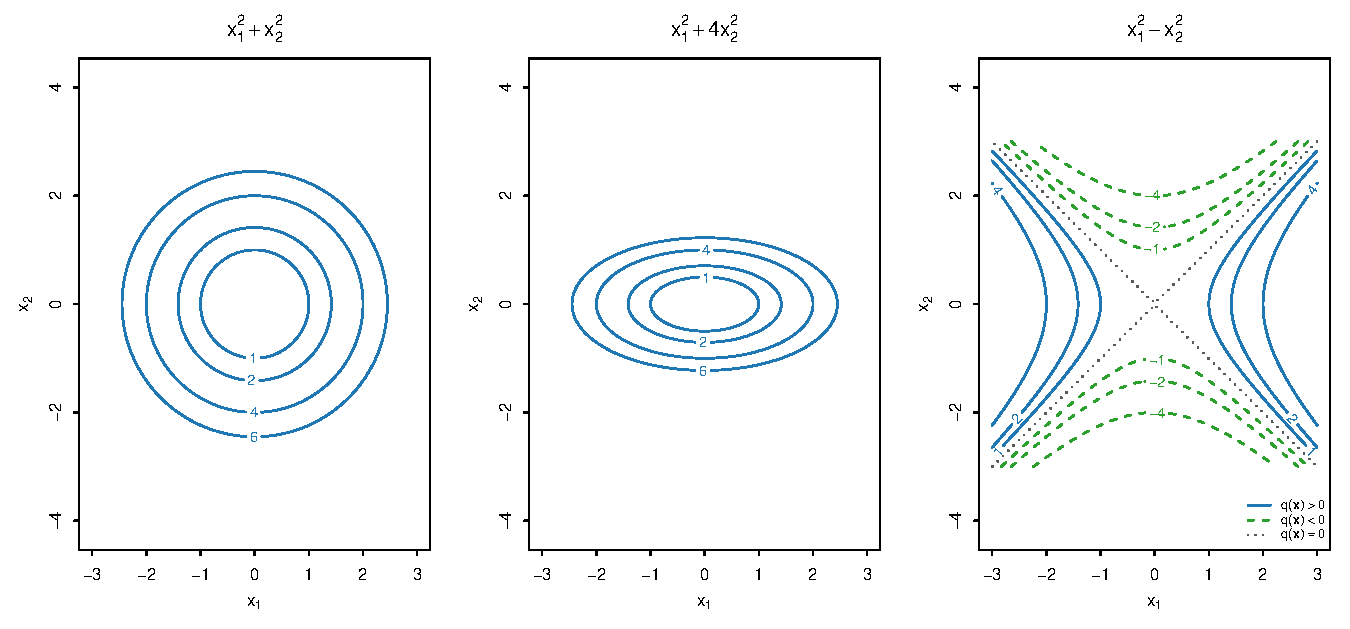
\includegraphics[keepaspectratio]{mod_1_matrizes_files/figure-pdf/fig-formas-quadraticas-1.pdf}}

}

\caption{\label{fig-formas-quadraticas}Curvas de nível de formas
quadráticas em duas dimensões. Na forma indefinida, níveis positivos,
negativos e nulos são diferenciados também pelo tipo de linha.}

\end{figure}%

A primeira forma produz circunferências. A segunda produz elipses com
eixos de comprimentos diferentes. A terceira produz hipérboles.

Formas quadráticas aparecem em expressões de distância, variância e
densidade. Os critérios baseados em autovalores serão apresentados no
capítulo sobre decomposição espectral.

\section{Aprofundamento: matrizes particionadas e complemento de
Schur}\label{aprofundamento-matrizes-particionadas-e-complemento-de-schur}

\begin{tcolorbox}[enhanced jigsaw, colback=white, breakable, bottomrule=.15mm, left=2mm, arc=.35mm, rightrule=.15mm, colframe=quarto-callout-note-color-frame, toprule=.15mm, leftrule=.75mm, opacityback=0]

\vspace{-3mm}\textbf{Leitura de aprofundamento}\vspace{3mm}

Esta seção pode ser utilizada como referência nos capítulos posteriores.
As operações por blocos e o complemento de Schur serão retomados no
estudo de covariâncias particionadas, distribuições condicionais,
regressão entre blocos e correlação canônica.

\end{tcolorbox}

Uma matriz pode ser dividida em submatrizes denominadas blocos. O
particionamento organiza os elementos sem alterar a matriz e permite
realizar operações matriciais utilizando os blocos.

\subsection{Matrizes particionadas}\label{matrizes-particionadas}

\begin{definition}[Matriz
particionada]\protect\hypertarget{def-matriz-particionada}{}\label{def-matriz-particionada}

Considere

\[
\mathbf{A}
\in
\mathbb{R}^{(m_1+m_2)\times(n_1+n_2)}.
\]

Um particionamento de \(\mathbf{A}\) em quatro blocos pode ser escrito
como

\[
\mathbf{A}
=
\begin{bmatrix}
\mathbf{A}_{11} & \mathbf{A}_{12}\\
\mathbf{A}_{21} & \mathbf{A}_{22}
\end{bmatrix},
\]

em que

\[
\mathbf{A}_{11}
\in
\mathbb{R}^{m_1\times n_1},
\qquad
\mathbf{A}_{12}
\in
\mathbb{R}^{m_1\times n_2},
\]

\[
\mathbf{A}_{21}
\in
\mathbb{R}^{m_2\times n_1},
\qquad
\mathbf{A}_{22}
\in
\mathbb{R}^{m_2\times n_2}.
\]

\end{definition}

Os blocos de uma mesma linha do particionamento possuem o mesmo número
de linhas. Os blocos de uma mesma coluna possuem o mesmo número de
colunas.

\begin{example}[Particionamento de uma
matriz]\protect\hypertarget{exm-matriz-particionada}{}\label{exm-matriz-particionada}

Considere

\[
\mathbf{A}
=
\begin{bmatrix}
1 & 2 & 3\\
4 & 5 & 6\\
7 & 8 & 9
\end{bmatrix}.
\]

Separando as duas primeiras linhas e colunas das restantes,

\[
\mathbf{A}
=
\left[
\begin{array}{cc|c}
1 & 2 & 3\\
4 & 5 & 6\\ \hline
7 & 8 & 9
\end{array}
\right]
=
\begin{bmatrix}
\mathbf{A}_{11} & \mathbf{A}_{12}\\
\mathbf{A}_{21} & \mathbf{A}_{22}
\end{bmatrix},
\]

com

\[
\mathbf{A}_{11}
=
\begin{bmatrix}
1 & 2\\
4 & 5
\end{bmatrix},
\qquad
\mathbf{A}_{12}
=
\begin{bmatrix}
3\\
6
\end{bmatrix},
\]

\[
\mathbf{A}_{21}
=
\begin{bmatrix}
7 & 8
\end{bmatrix},
\qquad
\mathbf{A}_{22}
=
\begin{bmatrix}
9
\end{bmatrix}.
\]

\end{example}

O particionamento pode ser definido de acordo com a organização do
problema. Em uma matriz de dados, por exemplo, as colunas podem ser
separadas em dois grupos de variáveis:

\[
\mathbf{X}
=
\left[
\mathbf{X}_1
\;
\mathbf{X}_2
\right],
\]

em que

\[
\mathbf{X}_1
\in
\mathbb{R}^{n\times p_1},
\qquad
\mathbf{X}_2
\in
\mathbb{R}^{n\times p_2}
\]

e

\[
p_1+p_2=p.
\]

\subsection{Soma e multiplicação por
escalar}\label{soma-e-multiplicauxe7uxe3o-por-escalar}

Considere matrizes com o mesmo particionamento:

\[
\mathbf{A}
=
\begin{bmatrix}
\mathbf{A}_{11} & \mathbf{A}_{12}\\
\mathbf{A}_{21} & \mathbf{A}_{22}
\end{bmatrix}
\]

e

\[
\mathbf{B}
=
\begin{bmatrix}
\mathbf{B}_{11} & \mathbf{B}_{12}\\
\mathbf{B}_{21} & \mathbf{B}_{22}
\end{bmatrix}.
\]

A soma pode ser realizada por blocos:

\[
\mathbf{A}+\mathbf{B}
=
\begin{bmatrix}
\mathbf{A}_{11}+\mathbf{B}_{11}
&
\mathbf{A}_{12}+\mathbf{B}_{12}\\
\mathbf{A}_{21}+\mathbf{B}_{21}
&
\mathbf{A}_{22}+\mathbf{B}_{22}
\end{bmatrix}.
\]

Para \(\alpha\in\mathbb{R}\),

\[
\alpha\mathbf{A}
=
\begin{bmatrix}
\alpha\mathbf{A}_{11}
&
\alpha\mathbf{A}_{12}\\
\alpha\mathbf{A}_{21}
&
\alpha\mathbf{A}_{22}
\end{bmatrix}.
\]

As operações exigem que os blocos correspondentes possuam as mesmas
dimensões.

\subsection{Transposição por
blocos}\label{transposiuxe7uxe3o-por-blocos}

A transposta de uma matriz particionada é

\[
\mathbf{A}^{\top}
=
\begin{bmatrix}
\mathbf{A}_{11}^{\top}
&
\mathbf{A}_{21}^{\top}\\
\mathbf{A}_{12}^{\top}
&
\mathbf{A}_{22}^{\top}
\end{bmatrix}.
\]

Os blocos situados fora da diagonal trocam de posição e são transpostos.

Se \(\mathbf{A}\) é simétrica, então

\[
\mathbf{A}_{11}^{\top}
=
\mathbf{A}_{11},
\qquad
\mathbf{A}_{22}^{\top}
=
\mathbf{A}_{22}
\]

e

\[
\mathbf{A}_{21}
=
\mathbf{A}_{12}^{\top}.
\]

Nesse caso, a matriz pode ser escrita como

\[
\mathbf{A}
=
\begin{bmatrix}
\mathbf{A}_{11}
&
\mathbf{A}_{12}\\
\mathbf{A}_{12}^{\top}
&
\mathbf{A}_{22}
\end{bmatrix}.
\]

\subsection{Multiplicação por
blocos}\label{multiplicauxe7uxe3o-por-blocos}

Considere

\[
\mathbf{A}
=
\begin{bmatrix}
\mathbf{A}_{11} & \mathbf{A}_{12}\\
\mathbf{A}_{21} & \mathbf{A}_{22}
\end{bmatrix}
\in
\mathbb{R}^{(m_1+m_2)\times(n_1+n_2)}
\]

e

\[
\mathbf{B}
=
\begin{bmatrix}
\mathbf{B}_{11} & \mathbf{B}_{12}\\
\mathbf{B}_{21} & \mathbf{B}_{22}
\end{bmatrix}
\in
\mathbb{R}^{(n_1+n_2)\times(r_1+r_2)},
\]

com

\[
\mathbf{B}_{11}
\in
\mathbb{R}^{n_1\times r_1},
\qquad
\mathbf{B}_{12}
\in
\mathbb{R}^{n_1\times r_2},
\]

\[
\mathbf{B}_{21}
\in
\mathbb{R}^{n_2\times r_1},
\qquad
\mathbf{B}_{22}
\in
\mathbb{R}^{n_2\times r_2}.
\]

O produto é

\[
\mathbf{A}\mathbf{B}
=
\begin{bmatrix}
\mathbf{A}_{11}\mathbf{B}_{11}
+
\mathbf{A}_{12}\mathbf{B}_{21}
&
\mathbf{A}_{11}\mathbf{B}_{12}
+
\mathbf{A}_{12}\mathbf{B}_{22}\\
\mathbf{A}_{21}\mathbf{B}_{11}
+
\mathbf{A}_{22}\mathbf{B}_{21}
&
\mathbf{A}_{21}\mathbf{B}_{12}
+
\mathbf{A}_{22}\mathbf{B}_{22}
\end{bmatrix}.
\]

A regra é a mesma utilizada no produto matricial, com os elementos
substituídos por blocos de dimensões compatíveis.

\begin{example}[Multiplicação de matrizes
particionadas]\protect\hypertarget{exm-produto-blocos}{}\label{exm-produto-blocos}

Considere

\[
\mathbf{A}
=
\left[
\begin{array}{cc|c}
1 & 2 & 1\\
0 & 1 & 3\\ \hline
2 & 0 & 4
\end{array}
\right]
=
\begin{bmatrix}
\mathbf{A}_{11} & \mathbf{A}_{12}\\
\mathbf{A}_{21} & \mathbf{A}_{22}
\end{bmatrix}
\]

e

\[
\mathbf{B}
=
\left[
\begin{array}{cc|c}
1 & 0 & 1\\
2 & 1 & 0\\ \hline
-1 & 2 & 3
\end{array}
\right]
=
\begin{bmatrix}
\mathbf{B}_{11} & \mathbf{B}_{12}\\
\mathbf{B}_{21} & \mathbf{B}_{22}
\end{bmatrix}.
\]

Os blocos da primeira linha do produto são

\[
\mathbf{A}_{11}\mathbf{B}_{11}
+
\mathbf{A}_{12}\mathbf{B}_{21}
=
\begin{bmatrix}
4 & 4\\
-1 & 7
\end{bmatrix}
\]

e

\[
\mathbf{A}_{11}\mathbf{B}_{12}
+
\mathbf{A}_{12}\mathbf{B}_{22}
=
\begin{bmatrix}
4\\
9
\end{bmatrix}.
\]

Os blocos da segunda linha são

\[
\mathbf{A}_{21}\mathbf{B}_{11}
+
\mathbf{A}_{22}\mathbf{B}_{21}
=
\begin{bmatrix}
-2 & 8
\end{bmatrix}
\]

e

\[
\mathbf{A}_{21}\mathbf{B}_{12}
+
\mathbf{A}_{22}\mathbf{B}_{22}
=
\begin{bmatrix}
14
\end{bmatrix}.
\]

Portanto,

\[
\mathbf{A}\mathbf{B}
=
\left[
\begin{array}{cc|c}
4 & 4 & 4\\
-1 & 7 & 9\\ \hline
-2 & 8 & 14
\end{array}
\right].
\]

\end{example}

As operações por blocos permitem manipular grupos de linhas e colunas
como unidades matriciais. O complemento de Schur utiliza essa estrutura
para representar a parcela de um bloco ajustada pelo outro.

\subsection{Complemento de Schur}\label{complemento-de-schur}

Matrizes particionadas permitem tratar uma matriz de grande dimensão a
partir de blocos menores. Em vários problemas, é útil eliminar um desses
blocos e estudar a estrutura que permanece no outro. O
\textbf{complemento de Schur} é a matriz que surge naturalmente nesse
processo de eliminação.

\begin{definition}[Complemento de
Schur]\protect\hypertarget{def-complemento-schur}{}\label{def-complemento-schur}

Considere a matriz quadrada particionada

\[
\mathbf{A}
=
\begin{bmatrix}
\mathbf{A}_{11} & \mathbf{A}_{12}\\
\mathbf{A}_{21} & \mathbf{A}_{22}
\end{bmatrix},
\]

em que

\[
\mathbf{A}_{11}\in\mathbb{R}^{p\times p},\qquad \mathbf{A}_{12}\in\mathbb{R}^{p\times q},
\]

\[
\mathbf{A}_{21}\in\mathbb{R}^{q\times p},\qquad \mathbf{A}_{22}\in\mathbb{R}^{q\times q}.
\]

Os blocos diagonais \(\mathbf{A}_{11}\) e \(\mathbf{A}_{22}\) são
quadrados. Quando um deles é invertível, podemos utilizá-lo para
eliminar os efeitos dos blocos fora da diagonal.

Se \(\mathbf{A}_{22}\) é invertível, o \textbf{complemento de Schur de}
\(\mathbf{A}_{22}\) em \(\mathbf{A}\) é

\[
\mathbf{A}_{11\cdot2}
=
\mathbf{A}_{11}
-
\mathbf{A}_{12}\mathbf{A}_{22}^{-1}\mathbf{A}_{21}.
\]

Se \(\mathbf{A}_{11}\) é invertível, o \textbf{complemento de Schur de}
\(\mathbf{A}_{11}\) em \(\mathbf{A}\) é

\[
\mathbf{A}_{22\cdot1}
=
\mathbf{A}_{22}
-
\mathbf{A}_{21}\mathbf{A}_{11}^{-1}\mathbf{A}_{12}.
\]

\end{definition}

O complemento \(\mathbf{A}_{11\cdot2}\) possui dimensão \(p\times p\),
enquanto \(\mathbf{A}_{22\cdot1}\) possui dimensão \(q\times q\).

A expressão pode ser compreendida como uma correção do bloco diagonal
original. Por exemplo,

\[
\mathbf{A}_{11\cdot2}
=
\mathbf{A}_{11}
-
\mathbf{A}_{12}\mathbf{A}_{22}^{-1}\mathbf{A}_{21}
\]

parte de \(\mathbf{A}_{11}\) e retira a parcela associada às relações
que passam pelo segundo bloco. Essa interpretação ficará mais clara ao
observarmos a eliminação por blocos.

\subsection{Eliminação por blocos}\label{eliminauxe7uxe3o-por-blocos}

Suponha que \(\mathbf{A}_{22}\) seja invertível. Queremos eliminar o
bloco \(\mathbf{A}_{12}\), isto é, produzir uma matriz equivalente cuja
posição superior direita seja ocupada por uma matriz nula.

Para isso, considere

\[
\mathbf{E}
=
\begin{bmatrix}
\mathbf{I}_p & -\mathbf{A}_{12}\mathbf{A}_{22}^{-1}\\
\mathbf{0} & \mathbf{I}_q
\end{bmatrix}.
\]

Multiplicando \(\mathbf{E}\) por \(\mathbf{A}\),

\[
\mathbf{E}\mathbf{A}
=
\begin{bmatrix}
\mathbf{I}_p & -\mathbf{A}_{12}\mathbf{A}_{22}^{-1}\\
\mathbf{0} & \mathbf{I}_q
\end{bmatrix}
\begin{bmatrix}
\mathbf{A}_{11} & \mathbf{A}_{12}\\
\mathbf{A}_{21} & \mathbf{A}_{22}
\end{bmatrix}.
\]

Efetuando o produto por blocos,

\[
\mathbf{E}\mathbf{A}
=
\begin{bmatrix}
\mathbf{A}_{11}-\mathbf{A}_{12}\mathbf{A}_{22}^{-1}\mathbf{A}_{21}
&
\mathbf{A}_{12}-\mathbf{A}_{12}\mathbf{A}_{22}^{-1}\mathbf{A}_{22}\\
\mathbf{A}_{21}
&
\mathbf{A}_{22}
\end{bmatrix}.
\]

Como \(\mathbf{A}_{22}^{-1}\mathbf{A}_{22}=\mathbf{I}_q\),

\[
\mathbf{E}\mathbf{A}
=
\begin{bmatrix}
\mathbf{A}_{11\cdot2} & \mathbf{0}\\
\mathbf{A}_{21} & \mathbf{A}_{22}
\end{bmatrix}.
\]

Portanto, o complemento de Schur aparece exatamente como o bloco que
permanece depois da eliminação de \(\mathbf{A}_{12}\) utilizando
\(\mathbf{A}_{22}\).

Como

\[
\mathbf{E}^{-1}
=
\begin{bmatrix}
\mathbf{I}_p & \mathbf{A}_{12}\mathbf{A}_{22}^{-1}\\
\mathbf{0} & \mathbf{I}_q
\end{bmatrix},
\]

também podemos escrever

\[
\mathbf{A}
=
\begin{bmatrix}
\mathbf{I}_p & \mathbf{A}_{12}\mathbf{A}_{22}^{-1}\\
\mathbf{0} & \mathbf{I}_q
\end{bmatrix}
\begin{bmatrix}
\mathbf{A}_{11\cdot2} & \mathbf{0}\\
\mathbf{A}_{21} & \mathbf{A}_{22}
\end{bmatrix}.
\]

Essa fatoração é consequência direta da eliminação por blocos.

Um caso simples ajuda a reconhecer a estrutura. Para uma matriz
\(2\times2\),

\[
\mathbf{A}
=
\begin{bmatrix}
a & b\\
c & d
\end{bmatrix},
\]

com \(d\neq0\), o complemento de Schur de \(d\) é

\[
a-bd^{-1}c.
\]

Como veremos a seguir,

\[
\det(\mathbf{A})
=
d\left(a-bd^{-1}c\right)
=
ad-bc,
\]

recuperando a expressão usual do determinante de uma matriz
\(2\times2\).

\begin{example}[Cálculo de um complemento de
Schur]\protect\hypertarget{exm-complemento-schur}{}\label{exm-complemento-schur}

Considere a matriz particionada

\[
\mathbf{A}
=
\begin{bmatrix}
\mathbf{A}_{11} & \mathbf{A}_{12}\\
\mathbf{A}_{21} & \mathbf{A}_{22}
\end{bmatrix},
\]

em que

\[
\mathbf{A}_{11}
=
\begin{bmatrix}
3 & 1\\
1 & 3
\end{bmatrix},
\qquad
\mathbf{A}_{12}
=
\begin{bmatrix}
1 & 0\\
0 & 1
\end{bmatrix},
\]

\[
\mathbf{A}_{21}
=
\begin{bmatrix}
1 & 0\\
0 & 1
\end{bmatrix},
\qquad
\mathbf{A}_{22}
=
\begin{bmatrix}
1 & 0\\
0 & 1
\end{bmatrix}.
\]

Como \(\mathbf{A}_{22}=\mathbf{I}_2\), tem-se
\(\mathbf{A}_{22}^{-1}=\mathbf{I}_2\). Logo,

\[
\begin{aligned}
\mathbf{A}_{11\cdot2}
&=
\mathbf{A}_{11}
-
\mathbf{A}_{12}\mathbf{A}_{22}^{-1}\mathbf{A}_{21}\\
&=
\begin{bmatrix}
3 & 1\\
1 & 3
\end{bmatrix}
-
\begin{bmatrix}
1 & 0\\
0 & 1
\end{bmatrix}\\
&=
\begin{bmatrix}
2 & 1\\
1 & 2
\end{bmatrix}.
\end{aligned}
\]

\end{example}

\subsection{Determinante de uma matriz
particionada}\label{determinante-de-uma-matriz-particionada}

A eliminação por blocos mostra uma das principais utilidades do
complemento de Schur: calcular o determinante de uma matriz particionada
utilizando determinantes de matrizes menores.

\begin{theorem}[Determinante e complemento de
Schur]\protect\hypertarget{thm-determinante-complemento-schur}{}\label{thm-determinante-complemento-schur}

Para

\[
\mathbf{A}
=
\begin{bmatrix}
\mathbf{A}_{11} & \mathbf{A}_{12}\\
\mathbf{A}_{21} & \mathbf{A}_{22}
\end{bmatrix},
\]

se \(\mathbf{A}_{22}\) é invertível, então

\[
\det(\mathbf{A})
=
\det(\mathbf{A}_{22})
\det(\mathbf{A}_{11\cdot2}).
\]

Se \(\mathbf{A}_{11}\) é invertível, então

\[
\det(\mathbf{A})
=
\det(\mathbf{A}_{11})
\det(\mathbf{A}_{22\cdot1}).
\]

(Boyd; Vandenberghe, 2004)

\end{theorem}

\begin{proof}
Suponha que \(\mathbf{A}_{22}\) seja invertível. Pela eliminação por
blocos apresentada anteriormente,

\[
\mathbf{E}\mathbf{A}
=
\begin{bmatrix}
\mathbf{A}_{11\cdot2} & \mathbf{0}\\
\mathbf{A}_{21} & \mathbf{A}_{22}
\end{bmatrix},
\]

com

\[
\mathbf{E}
=
\begin{bmatrix}
\mathbf{I}_p & -\mathbf{A}_{12}\mathbf{A}_{22}^{-1}\\
\mathbf{0} & \mathbf{I}_q
\end{bmatrix}.
\]

Como \(\mathbf{E}\) é triangular por blocos e possui matrizes identidade
na diagonal,

\[
\det(\mathbf{E})=1.
\]

Portanto,

\[
\det(\mathbf{E}\mathbf{A})=\det(\mathbf{A}).
\]

A matriz \(\mathbf{E}\mathbf{A}\) também é triangular por blocos. Assim,

\[
\det(\mathbf{E}\mathbf{A})
=
\det(\mathbf{A}_{11\cdot2})
\det(\mathbf{A}_{22}).
\]

Logo,

\[
\det(\mathbf{A})
=
\det(\mathbf{A}_{22})
\det(\mathbf{A}_{11\cdot2}).
\]

A segunda identidade é obtida de forma análoga, eliminando o bloco
\(\mathbf{A}_{21}\) a partir de \(\mathbf{A}_{11}\).
\end{proof}

No Exemplo~\ref{exm-complemento-schur},

\[
\det(\mathbf{A}_{22})=1
\]

e

\[
\det(\mathbf{A}_{11\cdot2})=3.
\]

Consequentemente,

\[
\det(\mathbf{A})=3.
\]

\subsection{Inversão em blocos}\label{inversuxe3o-em-blocos}

O complemento de Schur também permite obter a inversa de uma matriz
particionada. A origem da expressão pode ser entendida a partir da mesma
fatoração obtida pela eliminação por blocos.

Se \(\mathbf{A}_{22}\) é invertível,

\[
\mathbf{A}
=
\begin{bmatrix}
\mathbf{I}_p & \mathbf{A}_{12}\mathbf{A}_{22}^{-1}\\
\mathbf{0} & \mathbf{I}_q
\end{bmatrix}
\begin{bmatrix}
\mathbf{A}_{11\cdot2} & \mathbf{0}\\
\mathbf{A}_{21} & \mathbf{A}_{22}
\end{bmatrix}.
\]

Se \(\mathbf{A}_{11\cdot2}\) também é invertível, os dois fatores são
invertíveis. Como a inversa de um produto inverte a ordem dos fatores, a
inversa de \(\mathbf{A}\) pode ser construída a partir das inversas
dessas duas matrizes mais simples.

\begin{proposition}[Inversa em
blocos]\protect\hypertarget{prp-inversa-complemento-schur}{}\label{prp-inversa-complemento-schur}

Considere a matriz particionada

\[
\mathbf{A}
=
\begin{bmatrix}
\mathbf{A}_{11} & \mathbf{A}_{12}\\
\mathbf{A}_{21} & \mathbf{A}_{22}
\end{bmatrix}
\]

e o complemento de Schur de \(\mathbf{A}_{22}\) em \(\mathbf{A}\),

\[
\mathbf{A}_{11\cdot 2}
=
\mathbf{A}_{11}
-
\mathbf{A}_{12}
\mathbf{A}_{22}^{-1}
\mathbf{A}_{21}.
\]

Se \(\mathbf{A}_{22}\) e \(\mathbf{A}_{11\cdot 2}\) são invertíveis,
então

\[
\mathbf{A}^{-1}
=
\begin{bmatrix}
\mathbf{A}_{11\cdot 2}^{-1}
&
-\mathbf{A}_{11\cdot 2}^{-1}
\mathbf{A}_{12}
\mathbf{A}_{22}^{-1}
\\[4pt]
-\mathbf{A}_{22}^{-1}
\mathbf{A}_{21}
\mathbf{A}_{11\cdot 2}^{-1}
&
\mathbf{B}_{22}
\end{bmatrix},
\]

com o bloco \((2,2)\) dado por

\[
\mathbf{B}_{22}
=
\mathbf{A}_{22}^{-1}
+
\mathbf{A}_{22}^{-1}
\mathbf{A}_{21}
\mathbf{A}_{11\cdot 2}^{-1}
\mathbf{A}_{12}
\mathbf{A}_{22}^{-1}.
\]

(Boyd; Vandenberghe, 2004)

\end{proposition}

A expressão pode parecer extensa, mas sua estrutura é determinada pela
eliminação anterior. O bloco \(\mathbf{A}_{11\cdot2}^{-1}\) representa a
parte de \(\mathbf{A}_{11}\) que permanece depois da eliminação do
segundo bloco.

Uma expressão equivalente pode ser obtida utilizando
\(\mathbf{A}_{22\cdot1}\) quando \(\mathbf{A}_{11}\) e
\(\mathbf{A}_{22\cdot1}\) são invertíveis.

\subsection{Positividade e complemento de
Schur}\label{positividade-e-complemento-de-schur}

Outra aplicação importante ocorre em matrizes simétricas. O complemento
de Schur permite verificar a definição positiva de uma matriz
particionada por meio de matrizes de menor dimensão.

Considere

\[
\mathbf{A}
=
\begin{bmatrix}
\mathbf{A}_{11} & \mathbf{A}_{12}\\
\mathbf{A}_{12}^{\top} & \mathbf{A}_{22}
\end{bmatrix}.
\]

Para estudar se \(\mathbf{A}\) é positiva definida, consideramos sua
forma quadrática. Para \(\mathbf{x}\in\mathbb{R}^p\) e
\(\mathbf{y}\in\mathbb{R}^q\),

\[
\begin{aligned}
\begin{bmatrix}
\mathbf{x}\\
\mathbf{y}
\end{bmatrix}^{\top}
\mathbf{A}
\begin{bmatrix}
\mathbf{x}\\
\mathbf{y}
\end{bmatrix}
&=
\mathbf{x}^{\top}\mathbf{A}_{11}\mathbf{x}
+
2\mathbf{x}^{\top}\mathbf{A}_{12}\mathbf{y}
+
\mathbf{y}^{\top}\mathbf{A}_{22}\mathbf{y}.
\end{aligned}
\]

Quando \(\mathbf{A}_{22}\) é invertível, os termos envolvendo
\(\mathbf{y}\) podem ser reorganizados completando a forma quadrática:

\[
\begin{aligned}
&
\mathbf{x}^{\top}\mathbf{A}_{11}\mathbf{x}
+
2\mathbf{x}^{\top}\mathbf{A}_{12}\mathbf{y}
+
\mathbf{y}^{\top}\mathbf{A}_{22}\mathbf{y}\\
&\qquad=
\mathbf{x}^{\top}
\left(
\mathbf{A}_{11}
-
\mathbf{A}_{12}\mathbf{A}_{22}^{-1}\mathbf{A}_{12}^{\top}
\right)
\mathbf{x}\\
&\qquad\quad+
\left(
\mathbf{y}
+
\mathbf{A}_{22}^{-1}\mathbf{A}_{12}^{\top}\mathbf{x}
\right)^{\top}
\mathbf{A}_{22}
\left(
\mathbf{y}
+
\mathbf{A}_{22}^{-1}\mathbf{A}_{12}^{\top}\mathbf{x}
\right).
\end{aligned}
\]

O primeiro termo contém exatamente o complemento de Schur de
\(\mathbf{A}_{22}\).

\begin{theorem}[Positividade e complemento de
Schur]\protect\hypertarget{thm-positividade-complemento-schur}{}\label{thm-positividade-complemento-schur}

Considere a matriz simétrica

\[
\mathbf{A}
=
\begin{bmatrix}
\mathbf{A}_{11} & \mathbf{A}_{12}\\
\mathbf{A}_{12}^{\top} & \mathbf{A}_{22}
\end{bmatrix}.
\]

Se \(\mathbf{A}_{22}\) é positiva definida, então \(\mathbf{A}\) é
positiva definida se, e somente se,

\[
\mathbf{A}_{11\cdot2}
=
\mathbf{A}_{11}
-
\mathbf{A}_{12}\mathbf{A}_{22}^{-1}\mathbf{A}_{12}^{\top}
\]

é positiva definida. (Boyd; Vandenberghe, 2004)

\end{theorem}

\begin{proof}
Pela decomposição da forma quadrática,

\[
\begin{aligned}
\begin{bmatrix}
\mathbf{x}\\
\mathbf{y}
\end{bmatrix}^{\top}
\mathbf{A}
\begin{bmatrix}
\mathbf{x}\\
\mathbf{y}
\end{bmatrix}
&=
\mathbf{x}^{\top}\mathbf{A}_{11\cdot2}\mathbf{x}\\
&\quad+
\left(
\mathbf{y}
+
\mathbf{A}_{22}^{-1}\mathbf{A}_{12}^{\top}\mathbf{x}
\right)^{\top}
\mathbf{A}_{22}
\left(
\mathbf{y}
+
\mathbf{A}_{22}^{-1}\mathbf{A}_{12}^{\top}\mathbf{x}
\right).
\end{aligned}
\]

Suponha inicialmente que \(\mathbf{A}_{11\cdot2}\) e \(\mathbf{A}_{22}\)
sejam positivas definidas.

Se \(\mathbf{x}\neq\mathbf{0}\), então

\[
\mathbf{x}^{\top}\mathbf{A}_{11\cdot2}\mathbf{x}>0,
\]

enquanto a segunda parcela é não negativa.

Se \(\mathbf{x}=\mathbf{0}\), então \(\mathbf{y}\neq\mathbf{0}\) e a
forma quadrática reduz-se a

\[
\mathbf{y}^{\top}\mathbf{A}_{22}\mathbf{y}>0.
\]

Logo, \(\mathbf{A}\) é positiva definida.

Reciprocamente, suponha que \(\mathbf{A}\) seja positiva definida. Para
qualquer \(\mathbf{x}\neq\mathbf{0}\), escolha

\[
\mathbf{y}
=
-\mathbf{A}_{22}^{-1}\mathbf{A}_{12}^{\top}\mathbf{x}.
\]

Com essa escolha, a segunda parcela da decomposição é igual a zero.
Portanto,

\[
\begin{bmatrix}
\mathbf{x}\\
\mathbf{y}
\end{bmatrix}^{\top}
\mathbf{A}
\begin{bmatrix}
\mathbf{x}\\
\mathbf{y}
\end{bmatrix}
=
\mathbf{x}^{\top}\mathbf{A}_{11\cdot2}\mathbf{x}>0.
\]

Assim, \(\mathbf{A}_{11\cdot2}\) é positiva definida.
\end{proof}

Uma condição equivalente pode ser formulada utilizando
\(\mathbf{A}_{11}\) e o complemento \(\mathbf{A}_{22\cdot1}\).

O complemento de Schur aparece sempre que uma matriz particionada é
estudada após a eliminação de um dos blocos. Por isso, ele será útil em
diferentes partes da Análise Multivariada.

Algebricamente, o termo

\[
\mathbf{A}_{12}\mathbf{A}_{22}^{-1}\mathbf{A}_{21}
\]

representa a correção associada ao segundo bloco, enquanto

\[
\mathbf{A}_{11\cdot2}
=
\mathbf{A}_{11}
-
\mathbf{A}_{12}\mathbf{A}_{22}^{-1}\mathbf{A}_{21}
\]

representa o primeiro bloco depois dessa correção.

Essa interpretação é puramente matricial e vale para matrizes
particionadas gerais.

Quando \(\mathbf{A}\) é uma matriz de covariâncias particionada,

\[
\mathbf{A}
=
\begin{bmatrix}
\mathbf{A}_{11} & \mathbf{A}_{12}\\
\mathbf{A}_{12}^{\top} & \mathbf{A}_{22}
\end{bmatrix},
\]

o complemento

\[
\mathbf{A}_{11}
-
\mathbf{A}_{12}\mathbf{A}_{22}^{-1}\mathbf{A}_{12}^{\top}
\]

adquire uma interpretação estatística adicional. Ele representa a matriz
de covariâncias da parcela do primeiro bloco que permanece após o ajuste
linear pelo segundo bloco. Sob normalidade conjunta, essa mesma matriz
corresponde à covariância condicional do primeiro bloco dado o segundo.

Essa estrutura será retomada no estudo de covariâncias condicionais,
regressão entre blocos e distribuição normal multivariada.

\section{Síntese do capítulo}\label{suxedntese-do-capuxedtulo-1}

Uma matriz organiza valores em linhas e colunas e permite representar
simultaneamente observações, variáveis, transformações e sistemas
lineares. As dimensões determinam quais operações são possíveis e qual
será a dimensão do resultado.

A tabela a seguir reúne os principais objetos desenvolvidos no capítulo.

\begin{longtable}[]{@{}
  >{\raggedright\arraybackslash}p{(\linewidth - 4\tabcolsep) * \real{0.3333}}
  >{\raggedright\arraybackslash}p{(\linewidth - 4\tabcolsep) * \real{0.3333}}
  >{\raggedright\arraybackslash}p{(\linewidth - 4\tabcolsep) * \real{0.3333}}@{}}
\caption{Principais objetos e operações matriciais desenvolvidos no
capítulo.}\label{tbl-sintese-algebra-matricial}\tabularnewline
\toprule\noalign{}
\begin{minipage}[b]{\linewidth}\raggedright
Objeto ou operação
\end{minipage} & \begin{minipage}[b]{\linewidth}\raggedright
Expressão ou condição
\end{minipage} & \begin{minipage}[b]{\linewidth}\raggedright
Interpretação e utilização
\end{minipage} \\
\midrule\noalign{}
\endfirsthead
\toprule\noalign{}
\begin{minipage}[b]{\linewidth}\raggedright
Objeto ou operação
\end{minipage} & \begin{minipage}[b]{\linewidth}\raggedright
Expressão ou condição
\end{minipage} & \begin{minipage}[b]{\linewidth}\raggedright
Interpretação e utilização
\end{minipage} \\
\midrule\noalign{}
\endhead
\bottomrule\noalign{}
\endlastfoot
Produto matriz-vetor & \(\mathbf{A}\mathbf{x}\) & Produz produtos
internos pelas linhas e combinações lineares pelas colunas \\
Produto matricial & \(\mathbf{A}_{n\times p}\mathbf{B}_{p\times r}\) &
Combina linhas e colunas de matrizes com dimensões compatíveis \\
Transposta &
\((\mathbf{A}\mathbf{B})^\top=\mathbf{B}^\top\mathbf{A}^\top\) & Troca
linhas por colunas e reorganiza produtos \\
Matriz simétrica & \(\mathbf{A}^\top=\mathbf{A}\) & Estrutura presente
em formas quadráticas e matrizes de covariâncias \\
Traço & \(\operatorname{tr}(\mathbf{A})=\sum_i a_{ii}\) & Resume a
diagonal e reorganiza expressões matriciais \\
Matriz inversa & \(\mathbf{A}^{-1}\mathbf{A}=\mathbf{I}_n\) & Reverte a
ação de uma matriz invertível \\
Determinante & \(\det(\mathbf{A})\) & Registra invertibilidade,
alteração de volume e orientação \\
Posto & \(\operatorname{posto}(\mathbf{A})\) & Mede a dimensão da
informação linearmente independente \\
Matriz ortogonal & \(\mathbf{Q}^\top\mathbf{Q}=\mathbf{I}_n\) & Preserva
produtos internos, normas e distâncias \\
Forma bilinear & \(\mathbf{x}^\top\mathbf{A}\mathbf{y}\) & Relaciona
dois vetores por meio de uma matriz \\
Forma quadrática & \(\mathbf{x}^\top\mathbf{A}\mathbf{x}\) & Representa
variâncias, distâncias e superfícies de nível \\
Complemento de Schur &
\(\mathbf{A}_{11}-\mathbf{A}_{12}\mathbf{A}_{22}^{-1}\mathbf{A}_{21}\) &
Elimina um bloco e produz um bloco reduzido \\
\end{longtable}

Para uma matriz quadrada

\[
\mathbf{A}
\in
\mathbb{R}^{n\times n},
\]

as condições

\[
\mathbf{A}
\text{ é invertível},
\]

\[
\det(\mathbf{A})\neq0
\]

e

\[
\operatorname{posto}(\mathbf{A})=n
\]

são equivalentes.

O posto também permite classificar as soluções do sistema

\[
\mathbf{A}\mathbf{x}
=
\mathbf{b}.
\]

Quando a matriz não é invertível ou não é quadrada, a pseudoinversa
permite formular soluções exatas de menor norma ou soluções de mínimos
quadrados.

Para uma matriz simétrica, os valores da forma quadrática

\[
\mathbf{x}^{\top}\mathbf{A}\mathbf{x}
\]

permitem classificá-la como positiva definida, semidefinida positiva,
negativa definida, semidefinida negativa ou indefinida.

As seções sobre pseudoinversa, sistemas triangulares, matrizes
particionadas e complemento de Schur funcionam como aprofundamentos.
Esses resultados serão retomados quando sua utilização estatística se
tornar necessária.

Ao final deste capítulo, o estudante deverá ser capaz de:

\begin{itemize}
\tightlist
\item
  verificar a compatibilidade dimensional das operações matriciais;
\item
  calcular e interpretar produtos matriz-vetor e matriz-matriz;
\item
  utilizar transposição, simetria e traço;
\item
  relacionar inversa, determinante e posto;
\item
  classificar as soluções de sistemas lineares;
\item
  reconhecer matrizes ortogonais, diagonais e triangulares;
\item
  calcular e interpretar formas bilineares e quadráticas;
\item
  classificar matrizes simétricas por meio de suas formas quadráticas;
\item
  operar com matrizes particionadas em situações introdutórias.
\end{itemize}

O próximo capítulo desenvolverá espaços vetoriais, bases, dimensão e
projeções, fornecendo uma interpretação geométrica mais ampla para o
posto, os sistemas lineares e as transformações matriciais.

\chapter{Espaços vetoriais, bases e
projeções}\label{espauxe7os-vetoriais-bases-e-projeuxe7uxf5es}

Os capítulos anteriores apresentaram a representação vetorial dos dados
e as operações matriciais utilizadas para manipulá-los. Neste capítulo,
os vetores são estudados como elementos de conjuntos que preservam as
operações de adição e multiplicação por escalar.

Essa estrutura permite identificar subespaços, verificar relações de
dependência linear e representar um espaço por meio de uma base. O posto
de uma matriz será interpretado a partir das dimensões de seus espaços
fundamentais.

A parte final do capítulo desenvolve a projeção ortogonal. Essa operação
decompõe um vetor em uma componente pertencente a um subespaço e uma
componente ortogonal, fornecendo a interpretação geométrica dos
problemas de melhor aproximação e mínimos quadrados.

\begin{tcolorbox}[enhanced jigsaw, colback=white, breakable, bottomrule=.15mm, left=2mm, arc=.35mm, rightrule=.15mm, colframe=quarto-callout-note-color-frame, toprule=.15mm, leftrule=.75mm, opacityback=0]

\vspace{-3mm}\textbf{Convenções para espaços vetoriais e subespaços}\vspace{3mm}

As convenções vetoriais e matriciais apresentadas nos capítulos
anteriores permanecem válidas. Neste capítulo, serão utilizadas também
as seguintes convenções:

\begin{itemize}
\tightlist
\item
  \(V\) e \(W\) representam espaços vetoriais ou subespaços vetoriais;
\item
  \(S\) representa, em geral, um subespaço de \(\mathbb{R}^p\);
\item
  \(\mathcal{B}\) representa uma base;
\item
  \(\mathcal{B}_W\) representa uma base associada ao subespaço \(W\);
\item
  \(\dim(V)\) representa a dimensão do espaço vetorial \(V\);
\item
  \(\operatorname{span}\{\mathbf{v}_1,\ldots,\mathbf{v}_k\}\) representa
  o subespaço gerado pelos vetores \(\mathbf{v}_1,\ldots,\mathbf{v}_k\);
\item
  \([\mathbf{x}]_{\mathcal{B}}\) representa o vetor de coordenadas de
  \(\mathbf{x}\) em relação à base \(\mathcal{B}\);
\item
  \(S^{\perp}\) representa o complemento ortogonal de \(S\);
\item
  \(\mathcal{C}(\mathbf{A})\) representa o espaço coluna de
  \(\mathbf{A}\);
\item
  \(\mathcal{L}(\mathbf{A})\) representa o espaço linha de
  \(\mathbf{A}\);
\item
  \(\mathcal{N}(\mathbf{A})\) representa o espaço nulo de
  \(\mathbf{A}\);
\item
  \(\mathcal{N}(\mathbf{A}^{\top})\) representa o espaço nulo de
  \(\mathbf{A}^{\top}\);
\item
  \(\oplus\) representa soma direta de subespaços;
\item
  \(\operatorname{proj}_{S}(\mathbf{x})\) representa a projeção
  ortogonal de \(\mathbf{x}\) sobre \(S\);
\item
  \(\mathbf{P}_{S}\) representa uma matriz de projeção ortogonal sobre
  \(S\);
\item
  \(\mathbf{G}\) representa, quando indicado, uma matriz de Gram.
\end{itemize}

Quando uma base for escrita como

\[
\mathcal{B}
=
\{
\mathbf{b}_1,\ldots,\mathbf{b}_k
\},
\]

a ordem dos vetores será considerada fixada sempre que forem utilizadas
coordenadas em relação a essa base.

Os vetores continuarão sendo representados por letras minúsculas em
negrito, como \(\mathbf{x}\), \(\mathbf{y}\) e \(\mathbf{v}\), enquanto
matrizes serão representadas por letras maiúsculas em negrito, como
\(\mathbf{A}\), \(\mathbf{B}\) e \(\mathbf{Q}\).

As definições e propriedades específicas de cada espaço, base,
decomposição ou operador serão apresentadas nas seções correspondentes.

\end{tcolorbox}

\section{Espaços, subespaços e
geração}\label{espauxe7os-subespauxe7os-e-gerauxe7uxe3o}

Um espaço vetorial é um conjunto no qual a soma de vetores e a
multiplicação por escalares permanecem definidas e satisfazem
propriedades algébricas específicas.

\begin{definition}[Espaço
vetorial]\protect\hypertarget{def-espaco-vetorial}{}\label{def-espaco-vetorial}

Um conjunto não vazio \(V\) é um \textbf{espaço vetorial real} quando
estão definidas:

\begin{itemize}
\tightlist
\item
  a soma \(\mathbf{x}+\mathbf{y}\in V\), para
  \(\mathbf{x},\mathbf{y}\in V\);
\item
  a multiplicação \(\alpha\mathbf{x}\in V\), para
  \(\alpha\in\mathbb{R}\) e \(\mathbf{x}\in V\);
\end{itemize}

e são satisfeitas as seguintes propriedades:

\begin{enumerate}
\def\labelenumi{\arabic{enumi}.}
\tightlist
\item
  Para quaisquer \(\mathbf{x},\mathbf{y}\in V\),
\end{enumerate}

\[\mathbf{x}+\mathbf{y}=\mathbf{y}+\mathbf{x}.\]

\begin{enumerate}
\def\labelenumi{\arabic{enumi}.}
\setcounter{enumi}{1}
\tightlist
\item
  Para quaisquer \(\mathbf{x},\mathbf{y},\mathbf{z}\in V\),
\end{enumerate}

\[(\mathbf{x}+\mathbf{y})+\mathbf{z}=\mathbf{x}+(\mathbf{y}+\mathbf{z}).\]

\begin{enumerate}
\def\labelenumi{\arabic{enumi}.}
\setcounter{enumi}{2}
\tightlist
\item
  Existe um vetor \(\mathbf{0}\in V\) tal que, para todo
  \(\mathbf{x}\in V\),
\end{enumerate}

\[\mathbf{x}+\mathbf{0}=\mathbf{x}.\]

\begin{enumerate}
\def\labelenumi{\arabic{enumi}.}
\setcounter{enumi}{3}
\tightlist
\item
  Para todo \(\mathbf{x}\in V\), existe um vetor \(-\mathbf{x}\in V\)
  tal que
\end{enumerate}

\[\mathbf{x}+(-\mathbf{x})=\mathbf{0}.\]

\begin{enumerate}
\def\labelenumi{\arabic{enumi}.}
\setcounter{enumi}{4}
\tightlist
\item
  Para quaisquer \(\mathbf{x},\mathbf{y}\in V\) e
  \(\alpha\in\mathbb{R}\),
\end{enumerate}

\[\alpha(\mathbf{x}+\mathbf{y})=\alpha\mathbf{x}+\alpha\mathbf{y}.\]

\begin{enumerate}
\def\labelenumi{\arabic{enumi}.}
\setcounter{enumi}{5}
\tightlist
\item
  Para quaisquer \(\mathbf{x}\in V\) e \(\alpha,\beta\in\mathbb{R}\),
\end{enumerate}

\[(\alpha+\beta)\mathbf{x}=\alpha\mathbf{x}+\beta\mathbf{x}.\]

\begin{enumerate}
\def\labelenumi{\arabic{enumi}.}
\setcounter{enumi}{6}
\tightlist
\item
  Para quaisquer \(\mathbf{x}\in V\) e \(\alpha,\beta\in\mathbb{R}\),
\end{enumerate}

\[\alpha(\beta\mathbf{x})=(\alpha\beta)\mathbf{x}.\]

\begin{enumerate}
\def\labelenumi{\arabic{enumi}.}
\setcounter{enumi}{7}
\tightlist
\item
  Para todo \(\mathbf{x}\in V\),
\end{enumerate}

\[1\mathbf{x}=\mathbf{x}.\]

\end{definition}

O espaço \(\mathbb{R}^p\), com as operações usuais de adição e
multiplicação por escalar, é um espaço vetorial. Seus elementos são
vetores com \(p\) componentes reais. O vetor nulo é

\[
\mathbf{0}
=
\begin{bmatrix}
0\\
\vdots\\
0
\end{bmatrix},
\]

e, para

\[
\mathbf{x}
=
\begin{bmatrix}
x_1\\
\vdots\\
x_p
\end{bmatrix},
\]

seu inverso aditivo é

\[
-\mathbf{x}
=
\begin{bmatrix}
-x_1\\
\vdots\\
-x_p
\end{bmatrix}.
\]

Os elementos de um espaço vetorial não precisam ser necessariamente
vetores numéricos. Por exemplo, o conjunto de todas as matrizes reais de
dimensão \(n\times p\),

\[\mathbb{R}^{n\times p},\]

também é um espaço vetorial com as operações usuais de adição de
matrizes e multiplicação por escalar. Nesse caso, os elementos do espaço
vetorial são matrizes.

\subsection{Subespaços vetoriais}\label{subespauxe7os-vetoriais}

Um subconjunto de um espaço vetorial pode preservar a estrutura das
operações.

\begin{definition}[Subespaço
vetorial]\protect\hypertarget{def-subespaco-vetorial}{}\label{def-subespaco-vetorial}

Seja \(V\) um espaço vetorial. Um subconjunto não vazio \(W\subseteq V\)
é um \textbf{subespaço vetorial} de \(V\) quando, para quaisquer
\(\mathbf{x},\mathbf{y}\in W\) e \(\alpha\in\mathbb{R}\),

\[
\mathbf{x}+\mathbf{y}
\in
W
\]

e

\[
\alpha\mathbf{x}
\in
W.
\]

\end{definition}

As duas condições garantem que toda combinação linear de vetores de
\(W\) também pertence a \(W\).

\begin{proposition}[Critério de
subespaço]\protect\hypertarget{prp-criterio-subespaco}{}\label{prp-criterio-subespaco}

Um subconjunto não vazio \(W\subseteq V\) é um subespaço vetorial se, e
somente se,

\[
\alpha\mathbf{x}
+
\beta\mathbf{y}
\in
W
\]

para quaisquer \(\mathbf{x},\mathbf{y}\in W\) e
\(\alpha,\beta\in\mathbb{R}\). (Meyer, 2023)

\end{proposition}

O vetor nulo pertence a todo subespaço. De fato, para qualquer
\(\mathbf{x}\in W\),

\[
0\mathbf{x}
=
\mathbf{0}
\in
W.
\]

\begin{example}[Reta que é um
subespaço]\protect\hypertarget{exm-reta-subespaco}{}\label{exm-reta-subespaco}

Considere

\[
W
=
\left\{
\begin{bmatrix}
t\\
t
\end{bmatrix}
:
t\in\mathbb{R}
\right\}
\subseteq
\mathbb{R}^2.
\]

Se

\[
\mathbf{x}
=
\begin{bmatrix}
t_1\\
t_1
\end{bmatrix}
\quad\text{e}\quad
\mathbf{y}
=
\begin{bmatrix}
t_2\\
t_2
\end{bmatrix}
\]

pertencem a \(W\), então

\[
\alpha\mathbf{x}
+
\beta\mathbf{y}
=
\begin{bmatrix}
\alpha t_1+\beta t_2\\
\alpha t_1+\beta t_2
\end{bmatrix}
\in
W.
\]

Portanto, \(W\) é um subespaço de \(\mathbb{R}^2\).

\end{example}

Uma reta que não passa pela origem não é um subespaço.

\begin{example}[Reta que não é um
subespaço]\protect\hypertarget{exm-reta-nao-subespaco}{}\label{exm-reta-nao-subespaco}

Considere

\[
S
=
\left\{
\begin{bmatrix}
t\\
t+1
\end{bmatrix}
:
t\in\mathbb{R}
\right\}.
\]

O vetor nulo não pertence a \(S\). Portanto, \(S\) não é um subespaço de
\(\mathbb{R}^2\).

Geometricamente, \(S\) é uma reta paralela a \(W\), mas deslocada e sem
passar pela origem.

\end{example}

A Figura~\ref{fig-subespaco} compara uma reta que é subespaço de
\(\mathbb{R}^2\) com uma reta paralela que não é subespaço.

\begin{figure}

\centering{

\pandocbounded{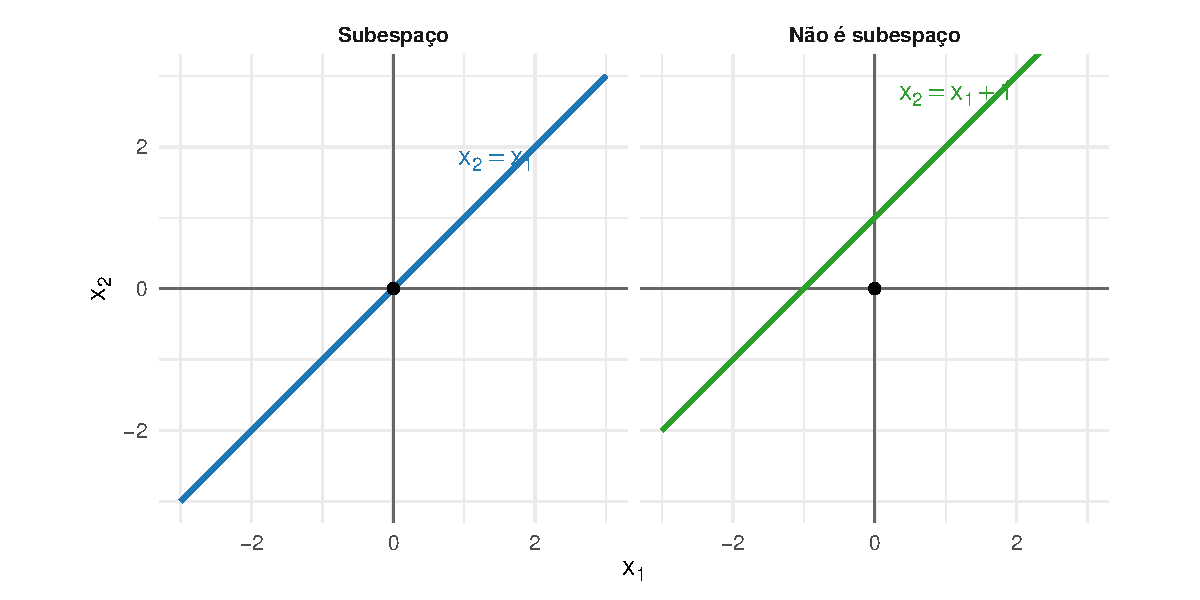
\includegraphics[keepaspectratio]{mod_1_espacos_files/figure-pdf/fig-subespaco-1.pdf}}

}

\caption{\label{fig-subespaco}Comparação entre uma reta que é subespaço
de \(\mathbb{R}^2\) e uma reta que não é subespaço.}

\end{figure}%

A reta do primeiro painel contém a origem e é fechada em relação às
combinações lineares. A reta do segundo painel não contém a origem e,
por isso, não é um subespaço de \(\mathbb{R}^2\).

\subsection{Subespaço gerado}\label{subespauxe7o-gerado}

As combinações lineares de um conjunto de vetores formam um subespaço.

\begin{definition}[Subespaço
gerado]\protect\hypertarget{def-subespaco-gerado}{}\label{def-subespaco-gerado}

Sejam

\[
\mathbf{v}_1,\mathbf{v}_2,\ldots,\mathbf{v}_k
\in
V.
\]

O \textbf{subespaço gerado} por esses vetores é o conjunto de todas as
suas combinações lineares,

\[
\operatorname{span}
\left\{
\mathbf{v}_1,\mathbf{v}_2,\ldots,\mathbf{v}_k
\right\}
=
\left\{
\alpha_1\mathbf{v}_1
+
\cdots
+
\alpha_k\mathbf{v}_k
:
\alpha_1,\ldots,\alpha_k\in\mathbb R
\right\}.
\]

A notação

\[
\operatorname{span}
\left\{
\mathbf{v}_1,\mathbf{v}_2,\ldots,\mathbf{v}_k
\right\}
\]

indica o subespaço gerado pelos vetores
\(\mathbf{v}_1,\ldots,\mathbf{v}_k\).

Esse conjunto também é denominado \textbf{envoltória linear} dos
vetores.

\end{definition}

O subespaço gerado é o menor subespaço que contém todos os vetores
\(\mathbf{v}_1,\ldots,\mathbf{v}_k\).

\begin{example}[Subespaço gerado por um
vetor]\protect\hypertarget{exm-subespaco-gerado-reta}{}\label{exm-subespaco-gerado-reta}

Considere

\[
\mathbf{v}
=
\begin{bmatrix}
1\\
2
\end{bmatrix}.
\]

O conjunto

\[
\operatorname{span}\{\mathbf{v}\}
=
\left\{
\alpha
\begin{bmatrix}
1\\
2
\end{bmatrix}
:
\alpha\in\mathbb{R}
\right\}
\]

é uma reta que passa pela origem.

\end{example}

\begin{example}[Subespaço gerado por dois
vetores]\protect\hypertarget{exm-subespaco-gerado-plano}{}\label{exm-subespaco-gerado-plano}

Considere

\[
\mathbf{v}_1
=
\begin{bmatrix}
1\\
0
\end{bmatrix},
\qquad
\mathbf{v}_2
=
\begin{bmatrix}
1\\
1
\end{bmatrix}.
\]

Uma combinação linear desses vetores é

\[
\alpha_1\mathbf{v}_1
+
\alpha_2\mathbf{v}_2
=
\begin{bmatrix}
\alpha_1+\alpha_2\\
\alpha_2
\end{bmatrix}.
\]

Para qualquer vetor

\[
\mathbf{x}
=
\begin{bmatrix}
x_1\\
x_2
\end{bmatrix}
\in
\mathbb{R}^2,
\]

basta escolher

\[
\alpha_2=x_2
\]

e

\[
\alpha_1=x_1-x_2.
\]

Portanto,

\[
\operatorname{span}
\{
\mathbf{v}_1,\mathbf{v}_2
\}
=
\mathbb{R}^2.
\]

\end{example}

\begin{example}[Espaço e subespaço
gerado]\protect\hypertarget{exm-comparacao-espaco-subespaco}{}\label{exm-comparacao-espaco-subespaco}

Considere o espaço vetorial

\[
V
=
\mathbb R^3.
\]

Primeiro, considere os vetores

\[
\mathbf{v}_1
=
\begin{bmatrix}
1\\
0\\
0
\end{bmatrix},
\qquad
\mathbf{v}_2
=
\begin{bmatrix}
0\\
1\\
0
\end{bmatrix},
\qquad
\mathbf{v}_3
=
\begin{bmatrix}
0\\
0\\
1
\end{bmatrix}.
\]

Uma combinação linear desses vetores é

\[
\alpha_1\mathbf{v}_1
+
\alpha_2\mathbf{v}_2
+
\alpha_3\mathbf{v}_3
=
\begin{bmatrix}
\alpha_1\\
\alpha_2\\
\alpha_3
\end{bmatrix}.
\]

Como qualquer vetor de \(\mathbb R^3\) pode ser obtido escolhendo
adequadamente \(\alpha_1\), \(\alpha_2\) e \(\alpha_3\),

\[
\operatorname{span}
\left\{
\mathbf{v}_1,
\mathbf{v}_2,
\mathbf{v}_3
\right\}
=
\mathbb R^3.
\]

Nesse caso, o subespaço gerado coincide com o próprio espaço \(V\).

Considere agora apenas os vetores

\[
\mathbf{v}_1
=
\begin{bmatrix}
1\\
0\\
0
\end{bmatrix},
\qquad
\mathbf{v}_2
=
\begin{bmatrix}
0\\
1\\
0
\end{bmatrix}.
\]

As combinações lineares desses vetores são da forma

\[
\alpha_1\mathbf{v}_1
+
\alpha_2\mathbf{v}_2
=
\begin{bmatrix}
\alpha_1\\
\alpha_2\\
0
\end{bmatrix}.
\]

Portanto,

\[
W
=
\operatorname{span}
\left\{
\mathbf{v}_1,
\mathbf{v}_2
\right\}
=
\left\{
\begin{bmatrix}
x_1\\
x_2\\
0
\end{bmatrix}
:
x_1,x_2\in\mathbb R
\right\}.
\]

O conjunto \(W\) é o plano \(x_3=0\) contido em \(\mathbb R^3\). Assim,

\[
W
\subsetneq
V,
\]

Os dois casos mostram que um subespaço gerado pode coincidir com todo o
espaço ou possuir dimensão menor. Em um espaço vetorial de dimensão
finita, um subespaço não pode ter dimensão maior que a do espaço que o
contém.

\end{example}

Um mesmo subespaço pode ser gerado por diferentes conjuntos de vetores.
Alguns conjuntos podem conter vetores redundantes. A independência
linear permite identificar quando um vetor acrescenta uma nova direção
ao subespaço gerado.

\section{Independência linear, bases e
dimensão}\label{independuxeancia-linear-bases-e-dimensuxe3o}

Um conjunto de vetores pode gerar um subespaço mesmo quando contém
vetores redundantes. A independência linear permite verificar se cada
vetor acrescenta uma nova direção ao conjunto gerado.

\subsection{Independência linear}\label{independuxeancia-linear}

\begin{definition}[Independência
linear]\protect\hypertarget{def-independencia-linear}{}\label{def-independencia-linear}

Os vetores

\[
\mathbf{v}_1,\mathbf{v}_2,\ldots,\mathbf{v}_k
\in
V
\]

são \textbf{linearmente independentes} quando a igualdade

\[
\alpha_1\mathbf{v}_1
+
\alpha_2\mathbf{v}_2
+
\cdots
+
\alpha_k\mathbf{v}_k
=
\mathbf{0}
\]

implica

\[
\alpha_1
=
\alpha_2
=
\cdots
=
\alpha_k
=
0.
\]

Quando existe uma solução em que pelo menos um coeficiente é diferente
de zero, os vetores são \textbf{linearmente dependentes}.

\end{definition}

A solução

\[
\alpha_1
=
\alpha_2
=
\cdots
=
\alpha_k
=
0
\]

é denominada \textbf{solução trivial}. Um conjunto é linearmente
independente quando a solução trivial é a única combinação linear que
produz o vetor nulo.

\begin{example}[Vetores linearmente
dependentes]\protect\hypertarget{exm-vetores-dependentes}{}\label{exm-vetores-dependentes}

Considere

\[
\mathbf{v}_1
=
\begin{bmatrix}
1\\
2
\end{bmatrix}
\qquad
\text{e}
\qquad
\mathbf{v}_2
=
\begin{bmatrix}
2\\
4
\end{bmatrix}.
\]

Como

\[
\mathbf{v}_2
=
2\mathbf{v}_1,
\]

tem-se

\[
2\mathbf{v}_1
-
\mathbf{v}_2
=
\mathbf{0}.
\]

Os coeficientes \(2\) e \(-1\) não são ambos nulos. Portanto,
\(\mathbf{v}_1\) e \(\mathbf{v}_2\) são linearmente dependentes.

Além disso,

\[
\operatorname{span}
\{
\mathbf{v}_1,\mathbf{v}_2
\}
=
\operatorname{span}
\{
\mathbf{v}_1
\}.
\]

O vetor \(\mathbf{v}_2\) não acrescenta uma nova direção ao subespaço
gerado.

\end{example}

\begin{example}[Vetores linearmente
independentes]\protect\hypertarget{exm-vetores-independentes}{}\label{exm-vetores-independentes}

Considere

\[
\mathbf{v}_1
=
\begin{bmatrix}
1\\
0
\end{bmatrix}
\qquad
\text{e}
\qquad
\mathbf{v}_2
=
\begin{bmatrix}
1\\
1
\end{bmatrix}.
\]

Suponha que

\[
\alpha_1\mathbf{v}_1
+
\alpha_2\mathbf{v}_2
=
\mathbf{0}.
\]

Então,

\[
\alpha_1
\begin{bmatrix}
1\\
0
\end{bmatrix}
+
\alpha_2
\begin{bmatrix}
1\\
1
\end{bmatrix}
=
\begin{bmatrix}
\alpha_1+\alpha_2\\
\alpha_2
\end{bmatrix}
=
\begin{bmatrix}
0\\
0
\end{bmatrix}.
\]

A segunda equação fornece

\[
\alpha_2=0,
\]

e a primeira fornece

\[
\alpha_1=0.
\]

Portanto, os vetores são linearmente independentes.

\end{example}

A Figura~\ref{fig-independencia-linear} compara dois vetores dependentes
com dois vetores independentes em \(\mathbb{R}^2\).

\begin{figure}

\centering{

\pandocbounded{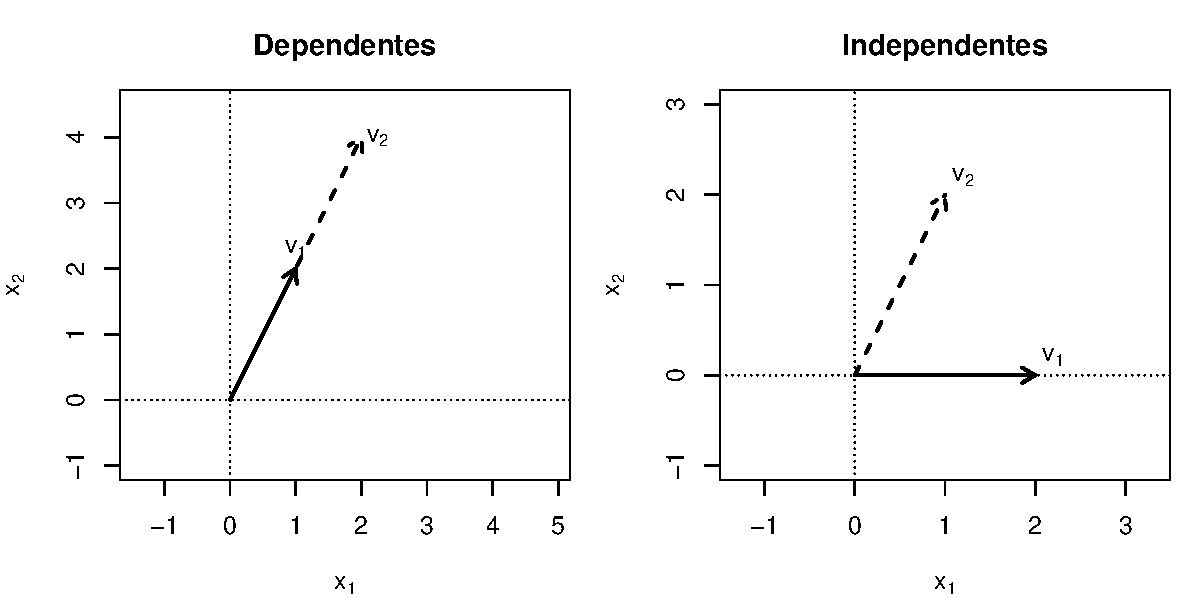
\includegraphics[keepaspectratio]{mod_1_espacos_files/figure-pdf/fig-independencia-linear-1.pdf}}

}

\caption{\label{fig-independencia-linear}Comparação entre vetores
linearmente dependentes e independentes em \(\mathbb{R}^2\).}

\end{figure}%

No primeiro painel, os vetores pertencem à mesma reta e geram um
subespaço unidimensional. No segundo, os vetores determinam duas
direções distintas e geram \(\mathbb{R}^2\).

\subsection{Independência linear e
posto}\label{independuxeancia-linear-e-posto}

Considere a matriz cujas colunas são os vetores analisados:

\[
\mathbf{A}
=
\begin{bmatrix}
\mathbf{v}_1
&
\mathbf{v}_2
&
\cdots
&
\mathbf{v}_k
\end{bmatrix},
\qquad
\mathbf{A}\in\mathbb{R}^{p\times k}.
\]

As colunas de \(\mathbf{A}\) são linearmente independentes se, e somente
se,

\[
\operatorname{posto}(\mathbf{A})
=
k.
\]

Assim, o número de vetores linearmente independentes entre as colunas de
\(\mathbf{A}\) é determinado pelo posto da matriz.

Como

\[
\operatorname{posto}(\mathbf{A})
\leq
\min(p,k),
\]

não pode haver mais de \(p\) vetores linearmente independentes em
\(\mathbb{R}^p\).

\begin{proposition}[Propriedades da independência
linear]\protect\hypertarget{prp-propriedades-independencia}{}\label{prp-propriedades-independencia}

Sejam \(\mathbf{v}_1,\ldots,\mathbf{v}_k\in V\).

\begin{enumerate}
\def\labelenumi{\arabic{enumi}.}
\item
  Um conjunto que contém o vetor nulo é linearmente dependente.
\item
  Um conjunto formado por um único vetor é linearmente independente se,
  e somente se, esse vetor é diferente de zero.
\item
  Todo subconjunto de um conjunto linearmente independente também é
  linearmente independente.
\item
  Todo conjunto que contém um subconjunto linearmente dependente é
  linearmente dependente.
\item
  Se um vetor do conjunto pode ser escrito como combinação linear dos
  demais, o conjunto é linearmente dependente.
\end{enumerate}

\end{proposition}

A última propriedade fornece uma interpretação direta da redundância.

\begin{proposition}[Dependência linear e
redundância]\protect\hypertarget{prp-dependencia-redundancia}{}\label{prp-dependencia-redundancia}

O conjunto

\[
\{
\mathbf{v}_1,\ldots,\mathbf{v}_k
\}
\]

é linearmente dependente se, e somente se, pelo menos um de seus vetores
pode ser escrito como combinação linear dos demais.

\end{proposition}

\begin{proof}
Suponha que o conjunto seja linearmente dependente. Então existem
coeficientes, não todos nulos, tais que

\[
\alpha_1\mathbf{v}_1
+
\cdots
+
\alpha_k\mathbf{v}_k
=
\mathbf{0}.
\]

Escolha um índice \(j\) para o qual \(\alpha_j\neq0\). Isolando
\(\mathbf{v}_j\),

\[
\mathbf{v}_j
=
-
\sum_{i\neq j}
\frac{\alpha_i}{\alpha_j}
\mathbf{v}_i.
\]

Portanto, \(\mathbf{v}_j\) é combinação linear dos demais.

Reciprocamente, se um vetor é combinação linear dos demais, essa
igualdade pode ser reorganizada como uma combinação linear não trivial
que produz o vetor nulo. Logo, o conjunto é linearmente dependente.
\end{proof}

A independência linear permite retirar vetores redundantes sem alterar o
subespaço gerado. Um conjunto gerador sem redundâncias fornece uma base
do subespaço.

\subsection{Bases}\label{bases}

Um conjunto gerador pode conter vetores redundantes. Quando os vetores
geram o espaço e são linearmente independentes, obtém-se uma base.

\begin{definition}[Base]\protect\hypertarget{def-base}{}\label{def-base}

Seja \(V\) um espaço vetorial. Um conjunto

\[
\mathcal{B}
=
\{
\mathbf{b}_1,\mathbf{b}_2,\ldots,\mathbf{b}_k
\}
\]

é uma \textbf{base} de \(V\) quando:

\begin{enumerate}
\def\labelenumi{\arabic{enumi}.}
\tightlist
\item
  os vetores \(\mathbf{b}_1,\ldots,\mathbf{b}_k\) são linearmente
  independentes;
\item
  os vetores geram \(V\), isto é,
\end{enumerate}

\[
\operatorname{span}
\{
\mathbf{b}_1,\ldots,\mathbf{b}_k
\}
=
V.
\]

\end{definition}

Uma base fornece um conjunto de vetores suficiente para gerar o espaço
sem incluir redundâncias.

\begin{example}[Uma base de
\(\mathbb{R}^2\)]\protect\hypertarget{exm-base-r2}{}\label{exm-base-r2}

Considere

\[
\mathbf{b}_1
=
\begin{bmatrix}
1\\
0
\end{bmatrix},
\qquad
\mathbf{b}_2
=
\begin{bmatrix}
1\\
1
\end{bmatrix}.
\]

Os vetores são linearmente independentes e geram \(\mathbb{R}^2\).
Portanto,

\[
\mathcal{B}
=
\{
\mathbf{b}_1,\mathbf{b}_2
\}
\]

é uma base de \(\mathbb{R}^2\).

\end{example}

Um mesmo espaço possui diferentes bases.

\begin{example}[Bases diferentes do mesmo
espaço]\protect\hypertarget{exm-bases-diferentes}{}\label{exm-bases-diferentes}

Os conjuntos

\[
\mathcal{B}_1
=
\left\{
\begin{bmatrix}
1\\
0
\end{bmatrix},
\begin{bmatrix}
0\\
1
\end{bmatrix}
\right\}
\]

e

\[
\mathcal{B}_2
=
\left\{
\begin{bmatrix}
1\\
1
\end{bmatrix},
\begin{bmatrix}
1\\
-1
\end{bmatrix}
\right\}
\]

são bases de \(\mathbb{R}^2\).

Os vetores de cada conjunto são linearmente independentes e geram todo o
espaço.

\end{example}

\subsection{Coordenadas em uma base}\label{coordenadas-em-uma-base}

Uma base permite representar cada vetor por meio dos coeficientes de sua
combinação linear.

\begin{theorem}[Representação única em uma
base]\protect\hypertarget{thm-representacao-unica-base}{}\label{thm-representacao-unica-base}

Se

\[
\mathcal{B}
=
\{
\mathbf{b}_1,\ldots,\mathbf{b}_k
\}
\]

é uma base de \(V\), então todo vetor \(\mathbf{x}\in V\) pode ser
escrito de maneira única como

\[
\mathbf{x}
=
c_1\mathbf{b}_1
+
\cdots
+
c_k\mathbf{b}_k.
\]

\end{theorem}

\begin{proof}
Como \(\mathcal{B}\) gera \(V\), existem escalares \(c_1,\ldots,c_k\)
tais que

\[
\mathbf{x}
=
c_1\mathbf{b}_1
+
\cdots
+
c_k\mathbf{b}_k.
\]

Suponha que também exista outra representação:

\[
\mathbf{x}
=
d_1\mathbf{b}_1
+
\cdots
+
d_k\mathbf{b}_k.
\]

Subtraindo as duas expressões,

\[
(c_1-d_1)\mathbf{b}_1
+
\cdots
+
(c_k-d_k)\mathbf{b}_k
=
\mathbf{0}.
\]

Como os vetores da base são linearmente independentes,

\[
c_i-d_i=0,
\qquad
i=1,\ldots,k.
\]

Portanto,

\[
c_i=d_i,
\qquad
i=1,\ldots,k,
\]

e a representação é única.
\end{proof}

\begin{definition}[Coordenadas em uma
base]\protect\hypertarget{def-coordenadas-base}{}\label{def-coordenadas-base}

Se

\[
\mathbf{x}
=
c_1\mathbf{b}_1
+
\cdots
+
c_k\mathbf{b}_k,
\]

o vetor

\[
[\mathbf{x}]_{\mathcal{B}}
=
\begin{bmatrix}
c_1\\
\vdots\\
c_k
\end{bmatrix}
\]

é o \textbf{vetor de coordenadas de} \(\mathbf{x}\) na base
\(\mathcal{B}\).

\end{definition}

Considere a matriz formada pelos vetores da base:

\[
\mathbf{B}
=
\begin{bmatrix}
\mathbf{b}_1
&
\cdots
&
\mathbf{b}_k
\end{bmatrix}.
\]

A representação de \(\mathbf{x}\) pode ser escrita como

\[
\mathbf{x}
=
\mathbf{B}
[\mathbf{x}]_{\mathcal{B}}.
\]

\begin{example}[Coordenadas de um
vetor]\protect\hypertarget{exm-coordenadas-base}{}\label{exm-coordenadas-base}

Considere a base

\[
\mathcal{B}
=
\left\{
\begin{bmatrix}
1\\
1
\end{bmatrix},
\begin{bmatrix}
1\\
-1
\end{bmatrix}
\right\}
\]

e o vetor

\[
\mathbf{x}
=
\begin{bmatrix}
4\\
2
\end{bmatrix}.
\]

Deseja-se determinar \(c_1\) e \(c_2\) tais que

\[
\begin{bmatrix}
4\\
2
\end{bmatrix}
=
c_1
\begin{bmatrix}
1\\
1
\end{bmatrix}
+
c_2
\begin{bmatrix}
1\\
-1
\end{bmatrix}.
\]

Isso produz o sistema

\[
\begin{aligned}
c_1+c_2 &= 4,\\
c_1-c_2 &= 2.
\end{aligned}
\]

Somando as equações,

\[
2c_1=6,
\]

de modo que

\[
c_1=3.
\]

Consequentemente,

\[
c_2=1.
\]

Logo,

\[
[\mathbf{x}]_{\mathcal{B}}
=
\begin{bmatrix}
3\\
1
\end{bmatrix}.
\]

\end{example}

As coordenadas dependem da base escolhida. O vetor permanece o mesmo,
mas os coeficientes que o representam podem mudar.

As coordenadas de um vetor em uma base são os coeficientes que indicam
quanto de cada vetor da base é necessário para reconstruir esse vetor
por combinação linear. Assim, o vetor de coordenadas não é o próprio
vetor, mas a representação desse vetor em relação à base escolhida.

\subsection{Base canônica}\label{base-canuxf4nica}

\begin{definition}[Base
canônica]\protect\hypertarget{def-base-canonica}{}\label{def-base-canonica}

A \textbf{base canônica} de \(\mathbb{R}^p\) é

\[
\mathcal{E}
=
\{
\mathbf{e}_1,\ldots,\mathbf{e}_p
\},
\]

em que \(\mathbf{e}_j\) possui valor \(1\) na posição \(j\) e valor
\(0\) nas demais posições.

\end{definition}

Em \(\mathbb{R}^3\),

\[
\mathbf{e}_1
=
\begin{bmatrix}
1\\
0\\
0
\end{bmatrix},
\qquad
\mathbf{e}_2
=
\begin{bmatrix}
0\\
1\\
0
\end{bmatrix},
\qquad
\mathbf{e}_3
=
\begin{bmatrix}
0\\
0\\
1
\end{bmatrix}.
\]

Para

\[
\mathbf{x}
=
\begin{bmatrix}
x_1\\
x_2\\
x_3
\end{bmatrix},
\]

tem-se

\[
\mathbf{x}
=
x_1\mathbf{e}_1
+
x_2\mathbf{e}_2
+
x_3\mathbf{e}_3.
\]

Assim, as coordenadas de \(\mathbf{x}\) na base canônica coincidem com
suas componentes usuais.

\subsection{Bases ortogonais e
ortonormais}\label{bases-ortogonais-e-ortonormais}

A partir deste ponto, considere um subespaço \(S\subseteq\mathbb{R}^p\)
com o produto interno euclidiano.

\begin{definition}[Base
ortogonal]\protect\hypertarget{def-base-ortogonal}{}\label{def-base-ortogonal}

Uma base

\[
\mathcal{B}
=
\{
\mathbf{b}_1,\ldots,\mathbf{b}_k
\}
\]

de \(S\) é \textbf{ortogonal} quando

\[\mathbf{b}_i^\top\mathbf{b}_j=0\qquad\text{para}\qquad i\neq j.\]

\end{definition}

\begin{definition}[Base
ortonormal]\protect\hypertarget{def-base-ortonormal}{}\label{def-base-ortonormal}

Uma base \(\mathcal{B}\) de \(S\) é \textbf{ortonormal} quando seus
vetores são ortogonais e possuem norma igual a \(1\):

\[
\mathbf{b}_i^\top\mathbf{b}_j
=
\begin{cases}
1, & i=j,\\
0, & i\neq j.
\end{cases}
\]

\end{definition}

Utilizando o delta de Kronecker, a condição de ortonormalidade pode ser
escrita como

\[\mathbf{b}_i^\top\mathbf{b}_j=\delta_{ij}.\] Se

\[
\mathbf{Q}
=
\begin{bmatrix}
\mathbf{b}_1
&
\cdots
&
\mathbf{b}_k
\end{bmatrix}
\]

possui como colunas os vetores de uma base ortonormal, então

\[
\mathbf{Q}^\top\mathbf{Q}
=
\mathbf{I}_k.
\]

Quando \(\mathbf{Q}\) é quadrada,

\[
\mathbf{Q}^{-1}
=
\mathbf{Q}^\top.
\]

Essa propriedade foi apresentada no capítulo anterior para matrizes
ortogonais.

\begin{theorem}[Existência de bases
ortonormais]\protect\hypertarget{thm-existencia-base-ortonormal}{}\label{thm-existencia-base-ortonormal}

Todo subespaço de dimensão finita de \(\mathbb{R}^p\) possui uma base
ortonormal.

A partir de qualquer base do subespaço, uma base ortonormal pode ser
construída pelo processo de ortogonalização de Gram--Schmidt. (Meyer,
2023)

\end{theorem}

Esse resultado garante que a geometria de um subespaço de dimensão
finita pode ser descrita por direções mutuamente ortogonais e de norma
unitária.

Em uma base ortogonal, os coeficientes da representação de um vetor
podem ser determinados separadamente.

\begin{proposition}[Coordenadas em uma base
ortogonal]\protect\hypertarget{prp-coordenadas-base-ortogonal}{}\label{prp-coordenadas-base-ortogonal}

Se

\[
\mathcal{B}
=
\{
\mathbf{b}_1,\ldots,\mathbf{b}_k
\}
\]

é uma base ortogonal de um subespaço \(S\subseteq\mathbb{R}^p\), então
todo vetor \(\mathbf{x}\in S\) pode ser escrito de maneira única como

\[\mathbf{x}=c_1\mathbf{b}_1+\cdots+c_k\mathbf{b}_k.\]

Cada coordenada de \(\mathbf{x}\) na base \(\mathcal{B}\) pode ser
obtida separadamente por

\[c_j=\frac{\mathbf{b}_j^\top\mathbf{x}}{\mathbf{b}_j^\top\mathbf{b}_j},\qquad j=1,\ldots,k.\]

Portanto,

\[
\mathbf{x}
=
\sum_{j=1}^{k}
\frac{\mathbf{b}_j^\top\mathbf{x}}
{\mathbf{b}_j^\top\mathbf{b}_j}
\mathbf{b}_j.
\]

Se a base é ortonormal, então \(\mathbf{b}_j^\top\mathbf{b}_j=1\) para
todo \(j\), de modo que

\[c_j=\mathbf{b}_j^\top\mathbf{x},\]

e

\[\mathbf{x}=\sum_{j=1}^{k}\left(\mathbf{b}_j^\top\mathbf{x}\right)\mathbf{b}_j.\]

Assim, em uma base ortogonal, cada coordenada pode ser determinada por
meio de um produto interno, sem a necessidade de resolver
simultaneamente um sistema linear. (Meyer, 2023)

\end{proposition}

\begin{proof}
Como \(\mathcal{B}\) é uma base de \(S\), todo vetor \(\mathbf{x}\in S\)
pode ser escrito de maneira única como

\[\mathbf{x}=c_1\mathbf{b}_1+\cdots+c_k\mathbf{b}_k.\]

Multiplicando ambos os lados à esquerda por \(\mathbf{b}_j^\top\),

\[
\mathbf{b}_j^\top\mathbf{x}
=
\sum_{i=1}^{k}
c_i\mathbf{b}_j^\top\mathbf{b}_i.
\]

Como a base é ortogonal,

\[\mathbf{b}_j^\top\mathbf{b}_i=0\qquad\text{para}\qquad i\neq j.\]

Assim, todos os termos da soma com \(i\neq j\) são nulos, restando

\[\mathbf{b}_j^\top\mathbf{x}=c_j\mathbf{b}_j^\top\mathbf{b}_j.\]

Como \(\mathbf{b}_j\neq\mathbf{0}\),

\[\mathbf{b}_j^\top\mathbf{b}_j=\|\mathbf{b}_j\|^2>0,\]

e, portanto,

\[c_j=\frac{\mathbf{b}_j^\top\mathbf{x}}{\mathbf{b}_j^\top\mathbf{b}_j}.\]

Se a base é ortonormal, então \(\|\mathbf{b}_j\|=1\) e,
consequentemente,

\[\mathbf{b}_j^\top\mathbf{b}_j=1.\]

Logo,

\[c_j=\mathbf{b}_j^\top\mathbf{x},\]

o que fornece diretamente as coordenadas de \(\mathbf{x}\) na base
ortonormal.
\end{proof}

A Figura~\ref{fig-bases-diferentes} compara três bases de
\(\mathbb{R}^2\) e destaca a diferença entre independência linear e
ortogonalidade.

\begin{figure}

\centering{

\pandocbounded{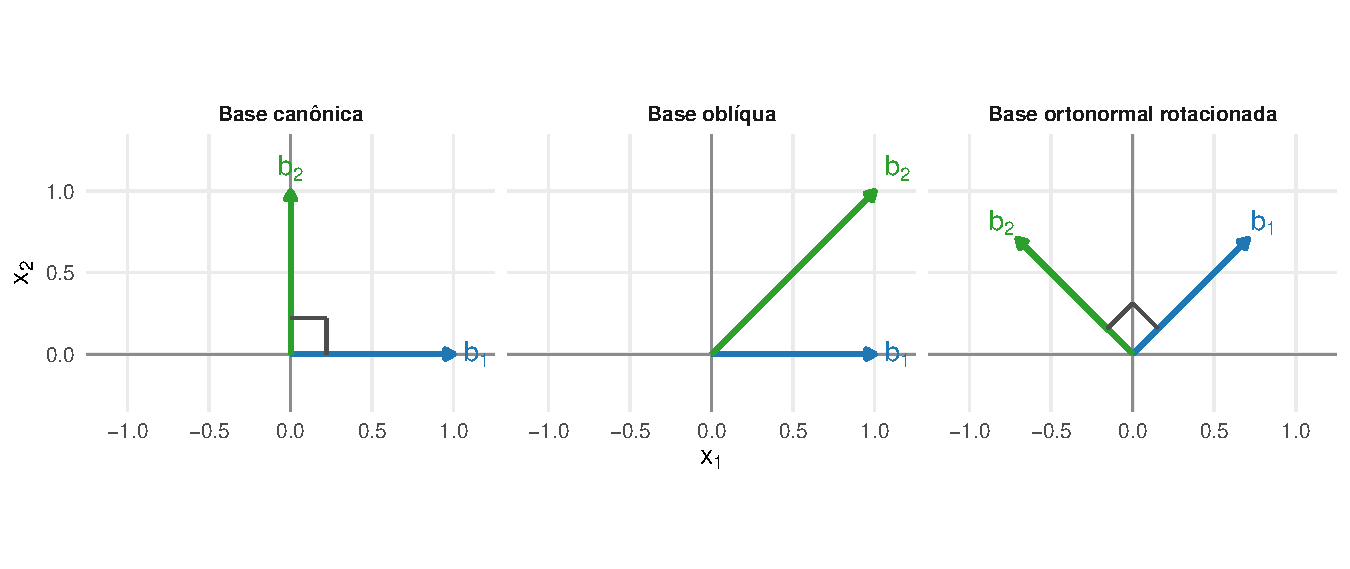
\includegraphics[keepaspectratio]{mod_1_espacos_files/figure-pdf/fig-bases-diferentes-1.pdf}}

}

\caption{\label{fig-bases-diferentes}Comparação entre uma base canônica,
uma base oblíqua e uma base ortonormal rotacionada de \(\mathbb{R}^2\).
O símbolo de ângulo reto identifica os pares de vetores ortogonais.}

\end{figure}%

Na primeira e na terceira bases, os vetores são ortogonais e possuem
norma igual a \(1\), como indicado pelos marcadores de ângulo reto.
Portanto, ambas são bases ortonormais. Na base oblíqua, os vetores
continuam sendo linearmente independentes e, por isso, formam uma base
de \(\mathbb{R}^2\), mas não são ortogonais.

\subsection{Dimensão}\label{dimensuxe3o}

Um espaço vetorial é denominado \textbf{finito-dimensional} quando
possui uma base formada por um número finito de vetores.

Para que a dimensão possa ser definida pelo número de vetores de uma
base, é necessário estabelecer primeiro que esse número não depende da
base escolhida.

\begin{theorem}[Número de vetores de uma
base]\protect\hypertarget{thm-cardinalidade-bases}{}\label{thm-cardinalidade-bases}

Se um espaço vetorial \(V\) possui uma base finita, então todas as bases
de \(V\) são finitas e possuem a mesma quantidade de vetores. (Meyer,
2023)

\end{theorem}

\begin{definition}[Dimensão]\protect\hypertarget{def-dimensao}{}\label{def-dimensao}

Se as bases de um espaço vetorial finito-dimensional \(V\) possuem \(k\)
vetores, a \textbf{dimensão} de \(V\) é definida por

\[\dim(V)=k.\]

\end{definition}

Como a base canônica de \(\mathbb{R}^p\) possui \(p\) vetores,

\[
\dim(\mathbb{R}^p)
=
p.
\]

\begin{example}[Dimensão de
subespaços]\protect\hypertarget{exm-dimensao-subespacos}{}\label{exm-dimensao-subespacos}

A reta

\[
W_1
=
\operatorname{span}
\left\{
\begin{bmatrix}
1\\
2\\
3
\end{bmatrix}
\right\}
\subseteq
\mathbb{R}^3
\]

possui dimensão \(1\).

O plano

\[
W_2
=
\operatorname{span}
\left\{
\begin{bmatrix}
1\\
0\\
0
\end{bmatrix},
\begin{bmatrix}
0\\
1\\
0
\end{bmatrix}
\right\}
\subseteq
\mathbb{R}^3
\]

possui dimensão \(2\).

O espaço \(\mathbb{R}^3\) possui dimensão \(3\).

\end{example}

\begin{proposition}[Independência, geração e
dimensão]\protect\hypertarget{prp-independencia-geracao-dimensao}{}\label{prp-independencia-geracao-dimensao}

Se \(\dim(V)=k\), então:

\begin{enumerate}
\def\labelenumi{\arabic{enumi}.}
\tightlist
\item
  qualquer conjunto com mais de \(k\) vetores é linearmente dependente;
\item
  qualquer conjunto com menos de \(k\) vetores não gera \(V\);
\item
  qualquer conjunto de \(k\) vetores linearmente independentes é uma
  base de \(V\);
\item
  qualquer conjunto de \(k\) vetores que gera \(V\) é uma base de \(V\).
\end{enumerate}

\end{proposition}

Esses resultados relacionam bases, independência e geração. Para uma
matriz, essa relação será expressa pelas dimensões de seus espaços
coluna, linha e nulo.

\section{Espaços fundamentais de uma
matriz}\label{espauxe7os-fundamentais-de-uma-matriz}

Uma matriz está associada a subespaços determinados por suas linhas, por
suas colunas e pelas soluções de sistemas lineares homogêneos. Esses
subespaços permitem relacionar o posto, a dependência linear e as
soluções de sistemas lineares.

Considere

\[
\mathbf A
\in
\mathbb R^{n\times p}.
\]

Serão estudados quatro subespaços associados a \(\mathbf A\):

\begin{itemize}
\tightlist
\item
  o espaço coluna;
\item
  o espaço linha;
\item
  o espaço nulo;
\item
  o espaço nulo à esquerda.
\end{itemize}

Os dois primeiros são construídos a partir das colunas e das linhas da
matriz. Os dois últimos são determinados pelas soluções dos sistemas
homogêneos associados, respectivamente, a \(\mathbf A\) e a
\(\mathbf A^{\top}\).

\subsection{Espaço nulo}\label{espauxe7o-nulo}

\begin{definition}[Espaço
nulo]\protect\hypertarget{def-espaco-nulo}{}\label{def-espaco-nulo}

O \textbf{espaço nulo} de uma matriz

\[
\mathbf{A}
\in
\mathbb{R}^{n\times p}
\]

é o conjunto

\[
\mathcal{N}(\mathbf{A})
=
\left\{
\mathbf{x}\in\mathbb{R}^p:
\mathbf{A}\mathbf{x}
=
\mathbf{0}
\right\}.
\]

Quando \(\mathbf{A}\) é interpretada como a matriz associada a uma
transformação linear, esse espaço corresponde ao \textbf{núcleo} da
transformação. Essa interpretação será formalizada no capítulo seguinte.

\end{definition}

O espaço nulo reúne todos os vetores \(\mathbf{x}\in\mathbb{R}^p\) que
são anulados pela multiplicação por \(\mathbf{A}\), isto é, aqueles para
os quais \(\mathbf{A}\mathbf{x}=\mathbf{0}\).

\begin{proposition}[O espaço nulo é um
subespaço]\protect\hypertarget{prp-espaco-nulo-subespaco}{}\label{prp-espaco-nulo-subespaco}

Para qualquer matriz

\[
\mathbf{A}
\in
\mathbb{R}^{n\times p},
\]

o conjunto

\[
\mathcal{N}(\mathbf{A})
\]

é um subespaço de \(\mathbb{R}^p\).

\end{proposition}

\begin{proof}
O vetor nulo pertence a \(\mathcal{N}(\mathbf{A})\), pois

\[
\mathbf{A}\mathbf{0}
=
\mathbf{0}.
\]

Se

\[
\mathbf{x},\mathbf{y}
\in
\mathcal{N}(\mathbf{A}),
\]

então

\[
\mathbf{A}\mathbf{x}
=
\mathbf{0}
\qquad
\text{e}
\qquad
\mathbf{A}\mathbf{y}
=
\mathbf{0}.
\]

Para quaisquer \(\alpha,\beta\in\mathbb{R}\),

\[
\begin{aligned}
\mathbf{A}
(
\alpha\mathbf{x}
+
\beta\mathbf{y}
)
&=
\alpha\mathbf{A}\mathbf{x}
+
\beta\mathbf{A}\mathbf{y}\\
&=
\alpha\mathbf{0}
+
\beta\mathbf{0}\\
&=
\mathbf{0}.
\end{aligned}
\]

Logo,

\[
\alpha\mathbf{x}
+
\beta\mathbf{y}
\in
\mathcal{N}(\mathbf{A}),
\]

e \(\mathcal{N}(\mathbf{A})\) é um subespaço.
\end{proof}

A dimensão do espaço nulo é denominada \textbf{nulidade} da matriz:

\[
\operatorname{nul}(\mathbf{A})
=
\dim
\mathcal{N}(\mathbf{A}).
\]

\begin{example}[Determinação do espaço
nulo]\protect\hypertarget{exm-espaco-nulo}{}\label{exm-espaco-nulo}

Considere

\[
\mathbf{A}
=
\begin{bmatrix}
1 & 2 & -1\\
2 & 4 & -2
\end{bmatrix}.
\]

Para determinar \(\mathcal{N}(\mathbf{A})\), resolve-se

\[
\mathbf{A}\mathbf{x}
=
\mathbf{0}.
\]

Assim,

\[
\begin{bmatrix}
1 & 2 & -1\\
2 & 4 & -2
\end{bmatrix}
\begin{bmatrix}
x_1\\
x_2\\
x_3
\end{bmatrix}
=
\begin{bmatrix}
0\\
0
\end{bmatrix}.
\]

As duas equações são equivalentes, e o sistema reduz-se a

\[
x_1+2x_2-x_3=0.
\]

Tomando

\[
x_2=s
\qquad
\text{e}
\qquad
x_3=t,
\]

obtém-se

\[
x_1=-2s+t.
\]

Portanto,

\[
\mathbf{x}
=
\begin{bmatrix}
-2s+t\\
s\\
t
\end{bmatrix}
=
s
\begin{bmatrix}
-2\\
1\\
0
\end{bmatrix}
+
t
\begin{bmatrix}
1\\
0\\
1
\end{bmatrix}.
\]

Logo,

\[
\mathcal{N}(\mathbf{A})
=
\operatorname{span}
\left\{
\begin{bmatrix}
-2\\
1\\
0
\end{bmatrix},
\begin{bmatrix}
1\\
0\\
1
\end{bmatrix}
\right\}.
\]

Os dois vetores são linearmente independentes. Assim,

\[
\operatorname{nul}(\mathbf{A})
=
2.
\]

\end{example}

Se

\[
\mathcal{N}(\mathbf{A})
=
\{\mathbf{0}\},
\]

as colunas de \(\mathbf{A}\) são linearmente independentes. Nesse caso,
o sistema homogêneo possui apenas a solução trivial.

\subsection{Espaço coluna}\label{espauxe7o-coluna}

\begin{definition}[Espaço
coluna]\protect\hypertarget{def-espaco-coluna}{}\label{def-espaco-coluna}

O \textbf{espaço coluna} de uma matriz

\[
\mathbf{A}
=
\begin{bmatrix}
\mathbf{a}_{\cdot1}
&
\mathbf{a}_{\cdot2}
&
\cdots
&
\mathbf{a}_{\cdot p}
\end{bmatrix}
\in
\mathbb{R}^{n\times p}
\]

é o subespaço

\[
\mathcal{C}(\mathbf{A})
=
\operatorname{span}
\left\{
\mathbf{a}_{\cdot1},
\ldots,
\mathbf{a}_{\cdot p}
\right\}
\subseteq
\mathbb{R}^n.
\]

\end{definition}

O produto matriz-vetor pode ser escrito como

\[
\mathbf{A}\mathbf{x}
=
x_1\mathbf{a}_{\cdot1}
+
\cdots
+
x_p\mathbf{a}_{\cdot p},
\qquad
\mathbf{x}\in\mathbb{R}^p.
\]

Portanto, todo vetor produzido por \(\mathbf{A}\) é uma combinação
linear de suas colunas.

Como

\[
\mathbf{A}\mathbf{x}
=
x_1\mathbf{a}_{\cdot1}
+
\cdots
+
x_p\mathbf{a}_{\cdot p},
\]

o conjunto de todos os vetores que podem ser escritos na forma
\(\mathbf{A}\mathbf{x}\) coincide com o espaço gerado pelas colunas de
\(\mathbf{A}\):

\[
\mathcal{C}(\mathbf{A})
=
\left\{
\mathbf{A}\mathbf{x}:
\mathbf{x}\in\mathbb{R}^p
\right\}.
\]

Essa caracterização permite relacionar diretamente o espaço coluna à
existência de soluções de sistemas lineares.

\begin{proposition}[Consistência de um sistema
linear]\protect\hypertarget{prp-consistencia-espaco-coluna}{}\label{prp-consistencia-espaco-coluna}

O sistema

\[
\mathbf{A}\mathbf{x}
=
\mathbf{b}
\]

possui pelo menos uma solução se, e somente se,

\[
\mathbf{b}
\in
\mathcal{C}(\mathbf{A}).
\]

\end{proposition}

\begin{proof}
Se o sistema possui uma solução \(\mathbf{x}\), então

\[
\mathbf{b}
=
\mathbf{A}\mathbf{x},
\]

de modo que \(\mathbf{b}\) é uma combinação linear das colunas de
\(\mathbf{A}\). Portanto,

\[
\mathbf{b}
\in
\mathcal{C}(\mathbf{A}).
\]

Reciprocamente, se

\[
\mathbf{b}
\in
\mathcal{C}(\mathbf{A}),
\]

existem escalares \(x_1,\ldots,x_p\) tais que

\[
\mathbf{b}
=
x_1\mathbf{a}_{\cdot1}
+
\cdots
+
x_p\mathbf{a}_{\cdot p}.
\]

Definindo

\[
\mathbf{x}
=
\begin{bmatrix}
x_1\\
\vdots\\
x_p
\end{bmatrix}
\in
\mathbb{R}^p,
\]

obtém-se

\[
\mathbf{A}\mathbf{x}
=
\mathbf{b}.
\]
\end{proof}

\begin{example}[Determinação do espaço
coluna]\protect\hypertarget{exm-espaco-coluna}{}\label{exm-espaco-coluna}

Considere novamente

\[
\mathbf{A}
=
\begin{bmatrix}
1 & 2 & -1\\
2 & 4 & -2
\end{bmatrix}.
\]

As colunas são

\[
\mathbf{a}_{\cdot1}
=
\begin{bmatrix}
1\\
2
\end{bmatrix},
\,\,
\mathbf{a}_{\cdot2}
=
\begin{bmatrix}
2\\
4
\end{bmatrix},
\,\,
\mathbf{a}_{\cdot3}
=
\begin{bmatrix}
-1\\
-2
\end{bmatrix}.
\]

Como

\[
\mathbf{a}_{\cdot2}
=
2\mathbf{a}_{\cdot1}
\]

e

\[
\mathbf{a}_{\cdot3}
=
-\mathbf{a}_{\cdot1},
\]

tem-se

\[
\mathcal{C}(\mathbf{A})
=
\operatorname{span}
\left\{
\begin{bmatrix}
1\\
2
\end{bmatrix}
\right\}.
\]

Logo,

\[
\dim
\mathcal{C}(\mathbf{A})
=
1.
\]

\end{example}

A dimensão do espaço coluna é igual ao posto da matriz:

\[
\dim
\mathcal{C}(\mathbf{A})
=
\operatorname{posto}(\mathbf{A}).
\]

Uma base de \(\mathcal{C}(\mathbf{A})\) pode ser formada por quaisquer
vetores linearmente independentes que gerem esse espaço. Quando se
deseja obter uma base selecionando colunas da própria matriz
\(\mathbf{A}\), as posições das colunas pivô podem ser identificadas por
escalonamento. Nesse procedimento, os vetores da base são as colunas
correspondentes da matriz original, e não as colunas da matriz
escalonada.

\subsection{Espaço linha}\label{espauxe7o-linha}

\begin{definition}[Espaço
linha]\protect\hypertarget{def-espaco-linha}{}\label{def-espaco-linha}

O \textbf{espaço linha} de uma matriz

\[
\mathbf{A}
\in
\mathbb{R}^{n\times p}
\]

é o subespaço de \(\mathbb{R}^p\) gerado por suas linhas.

Escrevendo as linhas de \(\mathbf{A}\) como

\[
\mathbf{a}_1^{\top},
\mathbf{a}_2^{\top},
\ldots,
\mathbf{a}_n^{\top},
\]

o espaço linha pode ser representado por

\[
\mathcal{L}(\mathbf{A})
=
\operatorname{span}
\left\{
\mathbf{a}_1,
\mathbf{a}_2,
\ldots,
\mathbf{a}_n
\right\}
\subseteq
\mathbb{R}^p.
\]

Equivalentemente, como as linhas de \(\mathbf{A}\) são as colunas de
\(\mathbf{A}^{\top}\),

\[
\mathcal{L}(\mathbf{A})
=
\mathcal{C}(\mathbf{A}^{\top}).
\]

\end{definition}

O espaço linha e o espaço coluna possuem a mesma dimensão:

\[
\dim
\mathcal{L}(\mathbf{A})
=
\dim
\mathcal{C}(\mathbf{A})
=
\operatorname{posto}(\mathbf{A}).
\]

Essa igualdade permite interpretar o posto tanto como o número máximo de
colunas linearmente independentes quanto como o número máximo de linhas
linearmente independentes.

\begin{example}[Determinação do espaço
linha]\protect\hypertarget{exm-espaco-linha}{}\label{exm-espaco-linha}

Considere

\[
\mathbf{A}
=
\begin{bmatrix}
1 & 2 & -1\\
2 & 4 & -2
\end{bmatrix}.
\]

As linhas de \(\mathbf{A}\) são

\[
\mathbf{a}_1^{\top}
=
\begin{bmatrix}
1 & 2 & -1
\end{bmatrix}
\]

e

\[
\mathbf{a}_2^{\top}
=
\begin{bmatrix}
2 & 4 & -2
\end{bmatrix}.
\]

Os vetores-coluna associados a essas linhas são

\[
\mathbf{a}_1
=
\begin{bmatrix}
1\\
2\\
-1
\end{bmatrix}
\qquad
\text{e}
\qquad
\mathbf{a}_2
=
\begin{bmatrix}
2\\
4\\
-2
\end{bmatrix}.
\]

Como

\[
\mathbf{a}_2
=
2\mathbf{a}_1,
\]

tem-se

\[
\mathcal{L}(\mathbf{A})
=
\operatorname{span}
\left\{
\begin{bmatrix}
1\\
2\\
-1
\end{bmatrix}
\right\}.
\]

Logo,

\[
\dim
\mathcal{L}(\mathbf{A})
=
1.
\]

\end{example}

As linhas não nulas de uma forma escalonada de \(\mathbf{A}\) formam uma
base de \(\mathcal{L}(\mathbf{A})\). Diferentemente do espaço coluna,
pode-se utilizar diretamente as linhas da matriz escalonada, pois as
operações elementares por linhas preservam o espaço linha.

\subsection{Espaço nulo à esquerda}\label{espauxe7o-nulo-uxe0-esquerda}

\begin{definition}[Espaço nulo à
esquerda]\protect\hypertarget{def-espaco-nulo-esquerda}{}\label{def-espaco-nulo-esquerda}

O \textbf{espaço nulo à esquerda} de

\[
\mathbf{A}
\in
\mathbb{R}^{n\times p}
\]

é definido por

\[
\mathcal{N}(\mathbf{A}^{\top})
=
\left\{
\mathbf{y}\in\mathbb{R}^n:
\mathbf{A}^{\top}\mathbf{y}
=
\mathbf{0}
\right\}.
\]

\end{definition}

Um vetor \(\mathbf{y}\) pertence a \(\mathcal{N}(\mathbf{A}^{\top})\)
quando é ortogonal a todas as colunas de \(\mathbf{A}\). De fato,

\[
\mathbf{A}^{\top}\mathbf{y}
=
\begin{bmatrix}
\mathbf{a}_{\cdot1}^{\top}\mathbf{y}\\
\mathbf{a}_{\cdot2}^{\top}\mathbf{y}\\
\vdots\\
\mathbf{a}_{\cdot p}^{\top}\mathbf{y}
\end{bmatrix}.
\]

Assim,

\[
\mathbf{A}^{\top}\mathbf{y}
=
\mathbf{0}
\]

se, e somente se,

\[
\mathbf{a}_{\cdot j}^{\top}\mathbf{y}
=
0,
\qquad
j=1,\ldots,p.
\]

Portanto, todo vetor de \(\mathcal{N}(\mathbf{A}^{\top})\) é ortogonal a
cada coluna de \(\mathbf{A}\) e, consequentemente, a toda combinação
linear dessas colunas. A relação entre o espaço nulo à esquerda e o
complemento ortogonal do espaço coluna será formalizada adiante.

\begin{example}[Determinação do espaço nulo à
esquerda]\protect\hypertarget{exm-espaco-nulo-esquerda}{}\label{exm-espaco-nulo-esquerda}

Considere novamente

\[
\mathbf{A}
=
\begin{bmatrix}
1 & 2 & -1\\
2 & 4 & -2
\end{bmatrix}.
\]

Para determinar \(\mathcal{N}(\mathbf{A}^{\top})\), resolve-se

\[
\mathbf{A}^{\top}\mathbf{y}
=
\mathbf{0}.
\]

Assim,

\[
\begin{bmatrix}
1 & 2\\
2 & 4\\
-1 & -2
\end{bmatrix}
\begin{bmatrix}
y_1\\
y_2
\end{bmatrix}
=
\begin{bmatrix}
0\\
0\\
0
\end{bmatrix}.
\]

O sistema reduz-se a

\[
y_1+2y_2=0.
\]

Tomando

\[
y_2=t,
\]

obtém-se

\[
y_1=-2t.
\]

Portanto,

\[
\mathbf{y}
=
t
\begin{bmatrix}
-2\\
1
\end{bmatrix},
\]

e

\[
\mathcal{N}(\mathbf{A}^{\top})
=
\operatorname{span}
\left\{
\begin{bmatrix}
-2\\
1
\end{bmatrix}
\right\}.
\]

Logo,

\[
\dim
\mathcal{N}(\mathbf{A}^{\top})
=
1.
\]

\end{example}

\subsection{Extensão de uma base}\label{extensuxe3o-de-uma-base}

Uma base de um subespaço pode ser completada acrescentando vetores até
formar uma base de todo o espaço. Esse resultado será utilizado na
demonstração do Teorema Posto--Nulidade.

\begin{theorem}[Extensão de uma
base]\protect\hypertarget{thm-extensao-base}{}\label{thm-extensao-base}

Seja \(W\) um subespaço de um espaço vetorial \(V\) de dimensão finita.
Se

\[
\mathcal{B}_W
=
\{
\mathbf{u}_1,\ldots,\mathbf{u}_s
\}
\]

é uma base de \(W\), então existem vetores
\(\mathbf{z}_1,\ldots,\mathbf{z}_r\in V\) tais que

\[
\{
\mathbf{u}_1,\ldots,\mathbf{u}_s,
\mathbf{z}_1,\ldots,\mathbf{z}_r
\}
\]

é uma base de \(V\). (Meyer, 2023)

\end{theorem}

\begin{proof}
Se \(\mathcal{B}_W\) já gera \(V\), então \(\mathcal{B}_W\) é uma base
de \(V\) e nada precisa ser acrescentado.

Caso contrário, existe um vetor \(\mathbf{z}_1\in V\) que não pertence
ao subespaço gerado por \(\mathcal{B}_W\). Assim,

\[
\{
\mathbf{u}_1,\ldots,\mathbf{u}_s,
\mathbf{z}_1
\}
\]

é linearmente independente.

Se esse conjunto ainda não gera \(V\), escolhe-se um vetor
\(\mathbf{z}_2\in V\) que não pertence ao subespaço gerado pelos vetores
já selecionados. O novo conjunto continua linearmente independente.

Repetindo esse procedimento, acrescentam-se vetores enquanto o conjunto
obtido não gerar \(V\). Como \(V\) possui dimensão finita, não é
possível acrescentar indefinidamente vetores linearmente independentes.
Portanto, após um número finito de etapas, obtém-se um conjunto

\[
\{
\mathbf{u}_1,\ldots,\mathbf{u}_s,
\mathbf{z}_1,\ldots,\mathbf{z}_r
\}
\]

que é linearmente independente e gera \(V\). Logo, esse conjunto é uma
base de \(V\).
\end{proof}

\subsection{Teorema Posto--Nulidade}\label{teorema-postonulidade}

As dimensões do espaço nulo e do espaço coluna estão relacionadas ao
número de colunas da matriz.

\begin{theorem}[Teorema
Posto--Nulidade]\protect\hypertarget{thm-posto-nulidade}{}\label{thm-posto-nulidade}

Se

\[
\mathbf{A}
\in
\mathbb{R}^{n\times p},
\]

então

\[
\operatorname{posto}(\mathbf{A})
+
\operatorname{nul}(\mathbf{A})
=
p.
\] (Meyer, 2023)

\end{theorem}

\begin{proof}
Considere uma base do espaço nulo,

\[
\mathcal{B}_{\mathcal{N}}
=
\{
\mathbf{v}_1,\ldots,\mathbf{v}_s
\},
\]

em que

\[s=\dim\mathcal{N}(\mathbf{A}).\]

Pelo Teorema~\ref{thm-extensao-base}, essa base de
\(\mathcal{N}(\mathbf{A})\) pode ser completada para formar uma base de
\(\mathbb{R}^p\). Assim, existem vetores
\(\mathbf{w}_1,\ldots,\mathbf{w}_r\in\mathbb{R}^p\) tais que

\[
\{
\mathbf{v}_1,\ldots,\mathbf{v}_s,
\mathbf{w}_1,\ldots,\mathbf{w}_r
\}
\]

é uma base de \(\mathbb{R}^p\).

Como essa base possui \(p\) vetores,

\[
s+r=p.
\]

Todo vetor \(\mathbf{x}\in\mathbb{R}^p\) possui uma representação da
forma

\[
\mathbf{x}
=
\sum_{i=1}^{s}
\alpha_i\mathbf{v}_i
+
\sum_{j=1}^{r}
\beta_j\mathbf{w}_j.
\]

Como

\[
\mathbf{A}\mathbf{v}_i
=
\mathbf{0},
\qquad
i=1,\ldots,s,
\]

tem-se

\[
\mathbf{A}\mathbf{x}
=
\sum_{j=1}^{r}
\beta_j
\mathbf{A}\mathbf{w}_j.
\]

Portanto,

\[
\mathbf{A}\mathbf{w}_1,\ldots,
\mathbf{A}\mathbf{w}_r
\]

geram \(\mathcal{C}(\mathbf{A})\).

Para verificar a independência linear, suponha que

\[
\sum_{j=1}^{r}
\beta_j
\mathbf{A}\mathbf{w}_j
=
\mathbf{0}.
\]

Então,

\[
\mathbf{A}
\left(
\sum_{j=1}^{r}
\beta_j\mathbf{w}_j
\right)
=
\mathbf{0},
\]

de modo que

\[
\sum_{j=1}^{r}
\beta_j\mathbf{w}_j
\in
\mathcal{N}(\mathbf{A}).
\]

Esse vetor também pertence a

\[
\operatorname{span}
\{
\mathbf{w}_1,\ldots,\mathbf{w}_r
\}.
\]

Como

\[
\{
\mathbf{v}_1,\ldots,\mathbf{v}_s,
\mathbf{w}_1,\ldots,\mathbf{w}_r
\}
\]

é uma base de \(\mathbb{R}^p\), a interseção entre esses dois subespaços
contém somente o vetor nulo. Assim,

\[
\beta_1
=
\cdots
=
\beta_r
=
0.
\]

Logo,

\[
\mathbf{A}\mathbf{w}_1,\ldots,
\mathbf{A}\mathbf{w}_r
\]

formam uma base de \(\mathcal{C}(\mathbf{A})\). Portanto,

\[
r
=
\dim
\mathcal{C}(\mathbf{A})
=
\operatorname{posto}(\mathbf{A}).
\]

Logo,

\[
\operatorname{posto}(\mathbf{A})
+
\dim
\mathcal{N}(\mathbf{A})
=
p.
\]
\end{proof}

Aplicando o teorema a \(\mathbf{A}^{\top}\),

\[
\operatorname{posto}(\mathbf{A}^{\top})
+
\dim
\mathcal{N}(\mathbf{A}^{\top})
=
n.
\]

Como

\[
\operatorname{posto}(\mathbf{A}^{\top})
=
\operatorname{posto}(\mathbf{A}),
\]

obtém-se

\[
\operatorname{posto}(\mathbf{A})
+
\dim
\mathcal{N}(\mathbf{A}^{\top})
=
n.
\]

\begin{example}[Aplicação do Teorema
Posto--Nulidade]\protect\hypertarget{exm-posto-nulidade}{}\label{exm-posto-nulidade}

Para a matriz utilizada nesta seção,

\[
\mathbf{A}
=
\begin{bmatrix}
1 & 2 & -1\\
2 & 4 & -2
\end{bmatrix},
\]

tem-se

\[\operatorname{posto}(\mathbf{A})=1,\]

\[\dim\mathcal{N}(\mathbf{A})=2\]

e

\[\dim\mathcal{N}(\mathbf{A}^{\top})=1.\]

Assim, para \(\mathbf{A}\in\mathbb{R}^{2\times 3}\),

\[1+2=3,\]

confirmando que

\[\operatorname{posto}(\mathbf{A})+\dim\mathcal{N}(\mathbf{A})=3.\]

Aplicando o resultado a \(\mathbf{A}^{\top}\),

\[1+1=2,\]

de modo que

\[\operatorname{posto}(\mathbf{A})+\dim\mathcal{N}(\mathbf{A}^{\top})=2.\]

Os resultados correspondem, respectivamente, às dimensões dos espaços
ambientes \(\mathbb{R}^3\) e \(\mathbb{R}^2\).

\end{example}

\subsection{Os quatro espaços
fundamentais}\label{os-quatro-espauxe7os-fundamentais}

Os quatro subespaços associados a

\[
\mathbf{A}
\in
\mathbb{R}^{n\times p}
\]

são:

\begin{longtable}[]{@{}
  >{\raggedright\arraybackslash}p{(\linewidth - 6\tabcolsep) * \real{0.2222}}
  >{\raggedright\arraybackslash}p{(\linewidth - 6\tabcolsep) * \real{0.5370}}
  >{\centering\arraybackslash}p{(\linewidth - 6\tabcolsep) * \real{0.1481}}
  >{\centering\arraybackslash}p{(\linewidth - 6\tabcolsep) * \real{0.0926}}@{}}
\caption{Espaços fundamentais de uma matriz
\(\mathbf{A}\in\mathbb{R}^{n\times p}\) com posto
\(r\).}\label{tbl-espacos-fundamentais}\tabularnewline
\toprule\noalign{}
\begin{minipage}[b]{\linewidth}\raggedright
Espaço
\end{minipage} & \begin{minipage}[b]{\linewidth}\raggedright
Definição
\end{minipage} & \begin{minipage}[b]{\linewidth}\centering
Subespaço de
\end{minipage} & \begin{minipage}[b]{\linewidth}\centering
Dimensão
\end{minipage} \\
\midrule\noalign{}
\endfirsthead
\toprule\noalign{}
\begin{minipage}[b]{\linewidth}\raggedright
Espaço
\end{minipage} & \begin{minipage}[b]{\linewidth}\raggedright
Definição
\end{minipage} & \begin{minipage}[b]{\linewidth}\centering
Subespaço de
\end{minipage} & \begin{minipage}[b]{\linewidth}\centering
Dimensão
\end{minipage} \\
\midrule\noalign{}
\endhead
\bottomrule\noalign{}
\endlastfoot
Espaço coluna & \(\mathcal{C}(\mathbf{A})\) & \(\mathbb{R}^n\) &
\(r\) \\
Espaço linha &
\(\mathcal{L}(\mathbf{A})=\mathcal{C}(\mathbf{A}^{\top})\) &
\(\mathbb{R}^p\) & \(r\) \\
Espaço nulo & \(\mathcal{N}(\mathbf{A})\) & \(\mathbb{R}^p\) &
\(p-r\) \\
Espaço nulo à esquerda & \(\mathcal{N}(\mathbf{A}^{\top})\) &
\(\mathbb{R}^n\) & \(n-r\) \\
\end{longtable}

A Tabela~\ref{tbl-espacos-fundamentais} mostra que os quatro espaços se
organizam em dois espaços ambientes. O espaço coluna e o espaço nulo à
esquerda são subespaços de \(\mathbb{R}^n\), enquanto o espaço linha e o
espaço nulo são subespaços de \(\mathbb{R}^p\).

\subsection{Complemento ortogonal}\label{complemento-ortogonal}

\begin{definition}[Complemento
ortogonal]\protect\hypertarget{def-complemento-ortogonal}{}\label{def-complemento-ortogonal}

Seja \(S\) um subespaço de \(\mathbb{R}^p\). O \textbf{complemento
ortogonal} de \(S\) é

\[
S^{\perp}
=
\left\{
\mathbf{x}\in\mathbb{R}^p:
\mathbf{x}^{\top}\mathbf{s}=0
\text{ para todo }
\mathbf{s}\in S
\right\}.
\]

\end{definition}

O complemento ortogonal reúne todos os vetores de \(\mathbb{R}^p\) que
são ortogonais a cada vetor de \(S\). Essa definição permite descrever
relações importantes entre os quatro espaços fundamentais de uma matriz.

\subsection{Relações de
ortogonalidade}\label{relauxe7uxf5es-de-ortogonalidade}

\begin{theorem}[Ortogonalidade entre os espaços
fundamentais]\protect\hypertarget{thm-ortogonalidade-espacos-fundamentais}{}\label{thm-ortogonalidade-espacos-fundamentais}

Para

\[
\mathbf{A}
\in
\mathbb{R}^{n\times p},
\]

tem-se

\[
\mathcal{N}(\mathbf{A})
=
\mathcal{L}(\mathbf{A})^{\perp}
\]

e

\[
\mathcal{N}(\mathbf{A}^{\top})
=
\mathcal{C}(\mathbf{A})^{\perp}.
\]

\end{theorem}

\begin{proof}
Considere inicialmente

\[
\mathbf{x}
\in
\mathcal{N}(\mathbf{A}).
\]

Então

\[
\mathbf{A}\mathbf{x}
=
\mathbf{0}.
\]

Cada componente de \(\mathbf{A}\mathbf{x}\) é o produto interno entre
uma linha de \(\mathbf{A}\) e \(\mathbf{x}\). Portanto, \(\mathbf{x}\) é
ortogonal a todas as linhas de \(\mathbf{A}\) e, consequentemente, a
todo vetor de \(\mathcal{L}(\mathbf{A})\). Logo,

\[
\mathbf{x}
\in
\mathcal{L}(\mathbf{A})^{\perp}.
\]

Assim,

\[
\mathcal{N}(\mathbf{A})
\subseteq
\mathcal{L}(\mathbf{A})^{\perp}.
\]

Reciprocamente, suponha que

\[
\mathbf{x}
\in
\mathcal{L}(\mathbf{A})^{\perp}.
\]

Então \(\mathbf{x}\) é ortogonal a todas as linhas de \(\mathbf{A}\).
Cada componente de \(\mathbf{A}\mathbf{x}\) é, portanto, igual a zero,
de modo que

\[
\mathbf{A}\mathbf{x}
=
\mathbf{0}.
\]

Logo,

\[
\mathbf{x}
\in
\mathcal{N}(\mathbf{A}),
\]

e

\[
\mathcal{L}(\mathbf{A})^{\perp}
\subseteq
\mathcal{N}(\mathbf{A}).
\]

Portanto,

\[
\mathcal{N}(\mathbf{A})
=
\mathcal{L}(\mathbf{A})^{\perp}.
\]

De forma análoga, para

\[
\mathbf{y}
\in
\mathbb{R}^n,
\]

a condição

\[
\mathbf{A}^{\top}\mathbf{y}
=
\mathbf{0}
\]

equivale a \(\mathbf{y}\) ser ortogonal a todas as colunas de
\(\mathbf{A}\). Portanto,

\[
\mathcal{N}(\mathbf{A}^{\top})
=
\mathcal{C}(\mathbf{A})^{\perp}.
\]
\end{proof}

Essas relações mostram que os espaços fundamentais se organizam em dois
pares ortogonais:

\[
\mathcal{L}(\mathbf{A})
\perp
\mathcal{N}(\mathbf{A})
\]

em \(\mathbb{R}^p\), e

\[
\mathcal{C}(\mathbf{A})
\perp
\mathcal{N}(\mathbf{A}^{\top})
\]

em \(\mathbb{R}^n\).

A decomposição dos espaços ambientes em somas diretas desses pares será
obtida posteriormente a partir do resultado geral sobre complementos
ortogonais.

\section{Produtos internos, bases ortonormais e matrizes de
Gram}\label{produtos-internos-bases-ortonormais-e-matrizes-de-gram}

O produto interno euclidiano

\[\langle\mathbf{x},\mathbf{y}\rangle=\mathbf{x}^{\top}\mathbf{y}\]

define comprimentos, ângulos e ortogonalidade em \(\mathbb{R}^p\). Além
da geometria euclidiana, é possível definir outras geometrias atribuindo
pesos e relações diferentes às coordenadas.

\subsection{Aprofundamento: produtos internos e geometrias
induzidas}\label{aprofundamento-produtos-internos-e-geometrias-induzidas}

\begin{tcolorbox}[enhanced jigsaw, colback=white, breakable, bottomrule=.15mm, left=2mm, arc=.35mm, rightrule=.15mm, colframe=quarto-callout-note-color-frame, toprule=.15mm, leftrule=.75mm, opacityback=0]

\vspace{-3mm}\textbf{Leitura de aprofundamento}\vspace{3mm}

Esta subseção generaliza o produto interno euclidiano por meio de
matrizes positivas definidas e apresenta as normas, distâncias e
relações de ortogonalidade associadas a essa generalização. Esses
conceitos serão retomados no estudo da distância de Mahalanobis, de
geometrias determinadas por matrizes de covariâncias e de problemas de
mínimos quadrados ponderados.

\end{tcolorbox}

Considere uma matriz simétrica positiva definida

\[\mathbf{M}\in\mathbb{R}^{p\times p}.\]

\begin{definition}[Produto interno induzido por uma
matriz]\protect\hypertarget{def-produto-interno-induzido}{}\label{def-produto-interno-induzido}

O \textbf{produto interno induzido por} \(\mathbf{M}\) é definido por

\[\langle\mathbf{x},\mathbf{y}\rangle_{\mathbf{M}}=\mathbf{x}^{\top}\mathbf{M}\mathbf{y},\qquad \mathbf{x},\mathbf{y}\in\mathbb{R}^p.\]

\end{definition}

A simetria de \(\mathbf{M}\) garante que

\[
\langle
\mathbf{x},
\mathbf{y}
\rangle_{\mathbf{M}}
=
\langle
\mathbf{y},
\mathbf{x}
\rangle_{\mathbf{M}},
\]

pois

\[
\mathbf{x}^{\top}
\mathbf{M}
\mathbf{y}
=
\left(
\mathbf{x}^{\top}
\mathbf{M}
\mathbf{y}
\right)^{\top}
=
\mathbf{y}^{\top}
\mathbf{M}^{\top}
\mathbf{x}
=
\mathbf{y}^{\top}
\mathbf{M}
\mathbf{x}.
\]

A definição positiva garante que

\[
\langle
\mathbf{x},
\mathbf{x}
\rangle_{\mathbf{M}}
=
\mathbf{x}^{\top}
\mathbf{M}
\mathbf{x}
>
0
\]

para todo \(\mathbf{x}\neq\mathbf{0}\).

\begin{proposition}[Propriedades do produto interno
induzido]\protect\hypertarget{prp-propriedades-produto-interno-induzido}{}\label{prp-propriedades-produto-interno-induzido}

Para quaisquer \(\mathbf{x},\mathbf{y},\mathbf{z}\in\mathbb{R}^p\) e
\(\alpha,\beta\in\mathbb{R}\),

\[\langle\mathbf{x},\mathbf{y}\rangle_{\mathbf{M}}=\langle\mathbf{y},\mathbf{x}\rangle_{\mathbf{M}},\]

\[\langle\alpha\mathbf{x}+\beta\mathbf{y},\mathbf{z}\rangle_{\mathbf{M}}=\alpha\langle\mathbf{x},\mathbf{z}\rangle_{\mathbf{M}}+\beta\langle\mathbf{y},\mathbf{z}\rangle_{\mathbf{M}},\]

e

\[\langle\mathbf{x},\mathbf{x}\rangle_{\mathbf{M}}>0\qquad\text{para}\qquad\mathbf{x}\neq\mathbf{0}.\]

(Horn; Johnson, 2013)

\end{proposition}

Quando

\[
\mathbf{M}
=
\mathbf{I}_p,
\]

recupera-se o produto interno euclidiano:

\[
\langle
\mathbf{x},
\mathbf{y}
\rangle_{\mathbf{I}_p}
=
\mathbf{x}^{\top}\mathbf{y}.
\]

\begin{example}[Cálculo de um produto interno
induzido]\protect\hypertarget{exm-produto-interno-induzido}{}\label{exm-produto-interno-induzido}

Considere

\[
\mathbf{M}
=
\begin{bmatrix}
2 & 1\\
1 & 2
\end{bmatrix},
\qquad
\mathbf{x}
=
\begin{bmatrix}
1\\
2
\end{bmatrix}
\]

e

\[
\mathbf{y}
=
\begin{bmatrix}
2\\
-1
\end{bmatrix}.
\]

Então,

\[
\mathbf{M}\mathbf{y}
=
\begin{bmatrix}
2 & 1\\
1 & 2
\end{bmatrix}
\begin{bmatrix}
2\\
-1
\end{bmatrix}
=
\begin{bmatrix}
3\\
0
\end{bmatrix}.
\]

Logo,

\[
\langle
\mathbf{x},
\mathbf{y}
\rangle_{\mathbf{M}}
=
\mathbf{x}^{\top}
\mathbf{M}
\mathbf{y}
=
\begin{bmatrix}
1 & 2
\end{bmatrix}
\begin{bmatrix}
3\\
0
\end{bmatrix}
=
3.
\]

O produto interno euclidiano entre os mesmos vetores é

\[
\mathbf{x}^{\top}\mathbf{y}
=
1(2)+2(-1)
=
0.
\]

Portanto, os vetores são ortogonais segundo o produto interno
euclidiano, mas não segundo o produto interno induzido por
\(\mathbf{M}\).

\end{example}

\subsubsection{Norma e distância
induzidas}\label{norma-e-distuxe2ncia-induzidas}

\begin{definition}[Norma
induzida]\protect\hypertarget{def-norma-induzida}{}\label{def-norma-induzida}

A norma associada ao produto interno induzido por \(\mathbf{M}\) é

\[\|\mathbf{x}\|_{\mathbf{M}}=\sqrt{\langle\mathbf{x},\mathbf{x}\rangle_{\mathbf{M}}}=\sqrt{\mathbf{x}^{\top}\mathbf{M}\mathbf{x}}.\]

\end{definition}

A distância associada é

\[d_{\mathbf{M}}(\mathbf{x},\mathbf{y})=\|\mathbf{x}-\mathbf{y}\|_{\mathbf{M}},\]

ou, equivalentemente,

\[d_{\mathbf{M}}(\mathbf{x},\mathbf{y})=\sqrt{(\mathbf{x}-\mathbf{y})^{\top}\mathbf{M}(\mathbf{x}-\mathbf{y})}.\]

Quando \(\mathbf{M}=\mathbf{I}_p\), obtêm-se a norma e a distância
euclidianas.

\begin{example}[Norma e distância
induzidas]\protect\hypertarget{exm-norma-distancia-induzidas}{}\label{exm-norma-distancia-induzidas}

Considere

\[
\mathbf{M}
=
\begin{bmatrix}
1 & 0\\
0 & 4
\end{bmatrix}
\]

e

\[
\mathbf{x}
=
\begin{bmatrix}
2\\
1
\end{bmatrix}.
\]

A norma euclidiana de \(\mathbf{x}\) é

\[
\|\mathbf{x}\|
=
\sqrt{2^2+1^2}
=
\sqrt{5}.
\]

A norma induzida por \(\mathbf{M}\) é

\[
\begin{aligned}
\|\mathbf{x}\|_{\mathbf{M}}
&=
\sqrt{
\begin{bmatrix}
2 & 1
\end{bmatrix}
\begin{bmatrix}
1 & 0\\
0 & 4
\end{bmatrix}
\begin{bmatrix}
2\\
1
\end{bmatrix}
}\\
&=
\sqrt{8}.
\end{aligned}
\]

A segunda coordenada recebe peso maior na geometria definida por
\(\mathbf{M}\).

\end{example}

\subsubsection{Ortogonalidade induzida}\label{ortogonalidade-induzida}

Dois vetores \(\mathbf{x}\) e \(\mathbf{y}\) são ortogonais segundo
\(\mathbf{M}\) quando

\[\langle\mathbf{x},\mathbf{y}\rangle_{\mathbf{M}}=\mathbf{x}^{\top}\mathbf{M}\mathbf{y}=0.\]

Uma base

\[
\mathcal{B}
=
\{
\mathbf{b}_1,\ldots,\mathbf{b}_k
\}
\]

é \(\mathbf{M}\)-ortonormal quando

\[\mathbf{b}_i^{\top}\mathbf{M}\mathbf{b}_j=\delta_{ij},\]

em que \(\delta_{ij}\) é o delta de Kronecker definido no capítulo
anterior.

Se

\[
\mathbf{B}
=
\begin{bmatrix}
\mathbf{b}_1 & \cdots & \mathbf{b}_k
\end{bmatrix},
\]

essa condição pode ser escrita como

\[\mathbf{B}^{\top}\mathbf{M}\mathbf{B}=\mathbf{I}_k.\]

\subsubsection{Relação com a geometria
euclidiana}\label{relauxe7uxe3o-com-a-geometria-euclidiana}

Como \(\mathbf{M}\) é simétrica positiva definida, existe uma matriz
invertível \(\mathbf{C}\) tal que

\[
\mathbf{M}
=
\mathbf{C}^{\top}\mathbf{C}.
\]

Assim,

\[
\begin{aligned}
\langle
\mathbf{x},
\mathbf{y}
\rangle_{\mathbf{M}}
&=
\mathbf{x}^{\top}
\mathbf{C}^{\top}
\mathbf{C}
\mathbf{y}\\
&=
(
\mathbf{C}\mathbf{x}
)^{\top}
(
\mathbf{C}\mathbf{y}
).
\end{aligned}
\]

Assim, o produto interno induzido por \(\mathbf{M}\) pode ser
interpretado como o produto interno euclidiano entre os vetores
\(\mathbf{C}\mathbf{x}\) e \(\mathbf{C}\mathbf{y}\). Da mesma forma,

\[
\|\mathbf{x}\|_{\mathbf{M}}
=
\|\mathbf{C}\mathbf{x}\|.
\]

As curvas de nível

\[
\|\mathbf{x}\|_{\mathbf{M}}
=
1
\]

satisfazem

\[
\mathbf{x}^{\top}
\mathbf{M}
\mathbf{x}
=
1.
\]

Na geometria euclidiana, essas curvas são circunferências quando
\(\mathbf{M}=\mathbf{I}_2\) e elipses para outras matrizes positivas
definidas.

A Figura~\ref{fig-geometrias-induzidas} compara três geometrias em
\(\mathbb{R}^2\).

\begin{figure}

\centering{

\pandocbounded{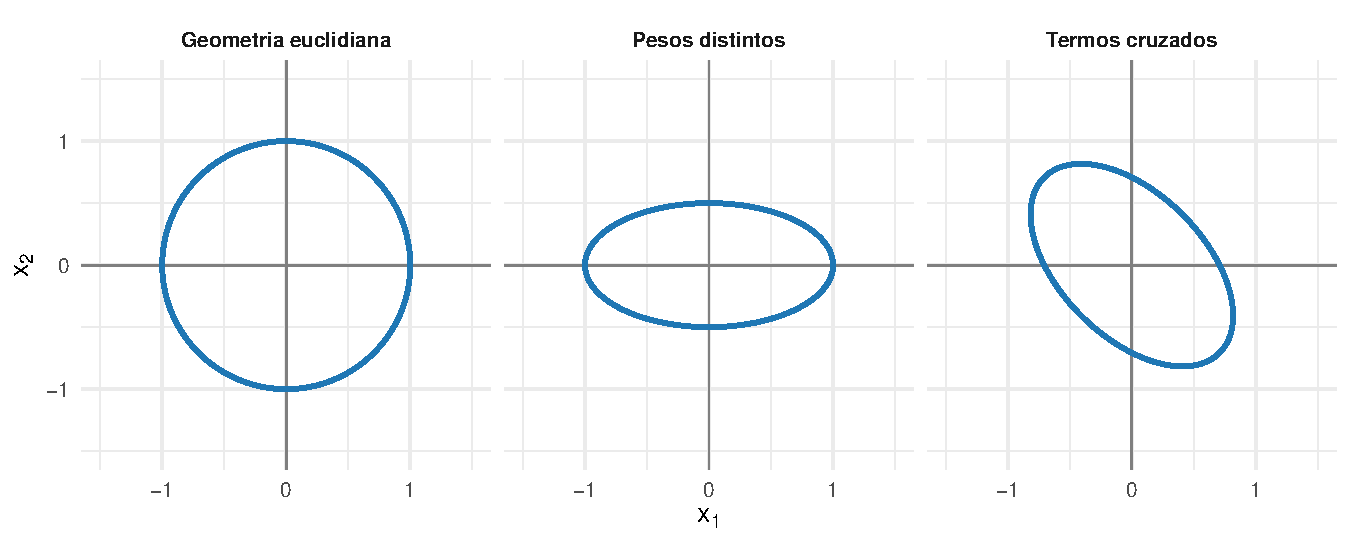
\includegraphics[keepaspectratio]{mod_1_espacos_files/figure-pdf/fig-geometrias-induzidas-1.pdf}}

}

\caption{\label{fig-geometrias-induzidas}Curvas de norma unitária para
diferentes produtos internos em \(\mathbb{R}^2\).}

\end{figure}%

A matriz identidade produz a circunferência euclidiana. Uma matriz
diagonal com pesos distintos produz uma elipse alinhada aos eixos
coordenados. Elementos fora da diagonal podem alterar a orientação da
elipse.

\begin{tcolorbox}[enhanced jigsaw, colback=white, breakable, bottomrule=.15mm, left=2mm, arc=.35mm, rightrule=.15mm, colframe=quarto-callout-caution-color-frame, toprule=.15mm, leftrule=.75mm, opacityback=0]

\vspace{-3mm}\textbf{Matrizes semidefinidas positivas}\vspace{3mm}

Se \(\mathbf{M}\) é apenas semidefinida positiva, a expressão

\[\|\mathbf{x}\|_{\mathbf{M}}=\sqrt{\mathbf{x}^{\top}\mathbf{M}\mathbf{x}}\]

pode ser igual a zero para algum vetor \(\mathbf{x}\neq\mathbf{0}\).

Nesse caso, a expressão define uma \textbf{seminorma}, e não uma norma.
Analogamente,

\[d_{\mathbf{M}}(\mathbf{x},\mathbf{y})=\|\mathbf{x}-\mathbf{y}\|_{\mathbf{M}}\]

pode ser igual a zero mesmo quando \(\mathbf{x}\neq\mathbf{y}\).
Portanto, essa expressão define, em geral, uma \textbf{pseudodistância}.

\end{tcolorbox}

Os produtos internos entre vários vetores podem ser organizados em uma
matriz de Gram.

\subsection{Matrizes de Gram}\label{matrizes-de-gram}

Os produtos internos entre um conjunto de vetores podem ser organizados
em uma matriz.

\begin{definition}[Matriz de
Gram]\protect\hypertarget{def-matriz-gram}{}\label{def-matriz-gram}

Sejam \(\mathbf{v}_1,\ldots,\mathbf{v}_k\in\mathbb{R}^p\) e

\[
\mathbf{V}
=
\begin{bmatrix}
\mathbf{v}_1 & \mathbf{v}_2 & \cdots & \mathbf{v}_k
\end{bmatrix}
\in
\mathbb{R}^{p\times k}.
\]

A \textbf{matriz de Gram} dos vetores é

\[\mathbf{G}=\mathbf{V}^{\top}\mathbf{V}.\]

Seu elemento na posição \((i,j)\) é

\[g_{ij}=\mathbf{v}_i^{\top}\mathbf{v}_j.\]

\end{definition}

A diagonal de \(\mathbf{G}\) contém os quadrados das normas:

\[
g_{ii}
=
\mathbf{v}_i^{\top}\mathbf{v}_i
=
\|\mathbf{v}_i\|^2.
\]

Os elementos fora da diagonal contêm os produtos internos entre vetores
distintos.

Quando \(\mathbf{v}_i\) e \(\mathbf{v}_j\) são não nulos,

\[
g_{ij}
=
\|\mathbf{v}_i\|
\|\mathbf{v}_j\|
\cos(\theta_{ij}).
\]

Portanto, o produto interno depende tanto das normas quanto do ângulo
entre os vetores.

\begin{example}[Construção de uma matriz de
Gram]\protect\hypertarget{exm-matriz-gram}{}\label{exm-matriz-gram}

Considere

\[
\mathbf{v}_1
=
\begin{bmatrix}
1\\
1\\
0
\end{bmatrix},
\qquad
\mathbf{v}_2
=
\begin{bmatrix}
1\\
0\\
1
\end{bmatrix}
\]

e

\[
\mathbf{V}
=
\begin{bmatrix}
1 & 1\\
1 & 0\\
0 & 1
\end{bmatrix}.
\]

A matriz de Gram é

\[
\begin{aligned}
\mathbf{G}
&=
\mathbf{V}^{\top}\mathbf{V}\\
&=
\begin{bmatrix}
1 & 1 & 0\\
1 & 0 & 1
\end{bmatrix}
\begin{bmatrix}
1 & 1\\
1 & 0\\
0 & 1
\end{bmatrix}\\
&=
\begin{bmatrix}
2 & 1\\
1 & 2
\end{bmatrix}.
\end{aligned}
\]

Os elementos diagonais são

\[
\|\mathbf{v}_1\|^2
=
\|\mathbf{v}_2\|^2
=
2,
\]

e o elemento fora da diagonal é

\[
\mathbf{v}_1^{\top}\mathbf{v}_2
=
1.
\]

\end{example}

\subsection{Propriedades da matriz de
Gram}\label{propriedades-da-matriz-de-gram}

\begin{proposition}[Propriedades da matriz de
Gram]\protect\hypertarget{prp-propriedades-matriz-gram}{}\label{prp-propriedades-matriz-gram}

Para

\[\mathbf{G}=\mathbf{V}^{\top}\mathbf{V},\]

tem-se:

\begin{enumerate}
\def\labelenumi{\arabic{enumi}.}
\tightlist
\item
  \(\mathbf{G}\) é simétrica;
\item
  \(\mathbf{G}\) é semidefinida positiva;
\item
  \(\mathbf{G}\) é positiva definida se, e somente se, as colunas de
  \(\mathbf{V}\) são linearmente independentes;
\item
  \(\operatorname{posto}(\mathbf{G})=\operatorname{posto}(\mathbf{V})\).
\end{enumerate}

(Horn; Johnson, 2013)

\end{proposition}

\begin{proof}
A simetria decorre de

\[\mathbf{G}^{\top}=(\mathbf{V}^{\top}\mathbf{V})^{\top}=\mathbf{V}^{\top}\mathbf{V}=\mathbf{G}.\]

Para qualquer \(\mathbf{c}\in\mathbb{R}^k\),

\[
\begin{aligned}
\mathbf{c}^{\top}\mathbf{G}\mathbf{c}
&=
\mathbf{c}^{\top}\mathbf{V}^{\top}\mathbf{V}\mathbf{c}\\
&=
(\mathbf{V}\mathbf{c})^{\top}(\mathbf{V}\mathbf{c})\\
&=
\|\mathbf{V}\mathbf{c}\|^2\\
&\geq
0.
\end{aligned}
\]

Logo, \(\mathbf{G}\) é semidefinida positiva.

Além disso,

\[\mathbf{c}^{\top}\mathbf{G}\mathbf{c}=0\]

se, e somente se,

\[\mathbf{V}\mathbf{c}=\mathbf{0}.\]

Portanto, \(\mathbf{G}\) é positiva definida se, e somente se, o sistema
homogêneo

\[\mathbf{V}\mathbf{c}=\mathbf{0}\]

possui apenas a solução trivial, o que equivale à independência linear
das colunas de \(\mathbf{V}\).

Para demonstrar a igualdade dos núcleos, suponha inicialmente que

\[\mathbf{V}^{\top}\mathbf{V}\mathbf{c}=\mathbf{0}.\]

Multiplicando à esquerda por \(\mathbf{c}^{\top}\),

\[\mathbf{c}^{\top}\mathbf{V}^{\top}\mathbf{V}\mathbf{c}=\|\mathbf{V}\mathbf{c}\|^2=0.\]

Logo,

\[\mathbf{V}\mathbf{c}=\mathbf{0},\]

e, portanto,

\[\mathcal{N}(\mathbf{V}^{\top}\mathbf{V})\subseteq\mathcal{N}(\mathbf{V}).\]

Reciprocamente, se

\[\mathbf{V}\mathbf{c}=\mathbf{0},\]

então

\[\mathbf{V}^{\top}\mathbf{V}\mathbf{c}=\mathbf{V}^{\top}\mathbf{0}=\mathbf{0},\]

de modo que

\[\mathcal{N}(\mathbf{V})\subseteq\mathcal{N}(\mathbf{V}^{\top}\mathbf{V}).\]

Assim,

\[\mathcal{N}(\mathbf{V}^{\top}\mathbf{V})=\mathcal{N}(\mathbf{V}).\]

Como \(\mathbf{V}^{\top}\mathbf{V}\) e \(\mathbf{V}\) possuem o mesmo
número de colunas, a igualdade das nulidades e o Teorema Posto--Nulidade
implicam

\[\operatorname{posto}(\mathbf{V}^{\top}\mathbf{V})=\operatorname{posto}(\mathbf{V}).\]
\end{proof}

Uma consequência é:

\[\det(\mathbf{V}^{\top}\mathbf{V})>0\]

se, e somente se, as colunas de \(\mathbf{V}\) são linearmente
independentes.

Quando as colunas são linearmente dependentes,

\[\det(\mathbf{V}^{\top}\mathbf{V})=0.\]

\subsection{Matrizes de Gram e bases
ortonormais}\label{matrizes-de-gram-e-bases-ortonormais}

Se as colunas de \(\mathbf{Q}\) formam um conjunto ortonormal, então

\[
\mathbf{Q}^{\top}\mathbf{Q}
=
\mathbf{I}.
\]

Portanto, a matriz de Gram de um conjunto ortonormal é a matriz
identidade.

Para uma base ortogonal não normalizada,

\[
\mathbf{V}^{\top}\mathbf{V}
=
\operatorname{diag}
\left(
\|\mathbf{v}_1\|^2,
\ldots,
\|\mathbf{v}_k\|^2
\right).
\]

\begin{example}[Matriz de Gram de uma base
ortogonal]\protect\hypertarget{exm-gram-base-ortogonal}{}\label{exm-gram-base-ortogonal}

Considere

\[
\mathbf{v}_1
=
\begin{bmatrix}
1\\
1
\end{bmatrix}
\qquad
\text{e}
\qquad
\mathbf{v}_2
=
\begin{bmatrix}
1\\
-1
\end{bmatrix}.
\]

Como

\[
\mathbf{v}_1^{\top}\mathbf{v}_2
=
0,
\]

os vetores são ortogonais.

A matriz de Gram é

\[
\mathbf{G}
=
\begin{bmatrix}
2 & 0\\
0 & 2
\end{bmatrix}.
\]

Normalizando os vetores,

\[
\mathbf{q}_1
=
\frac{1}{\sqrt{2}}
\begin{bmatrix}
1\\
1
\end{bmatrix},
\qquad
\mathbf{q}_2
=
\frac{1}{\sqrt{2}}
\begin{bmatrix}
1\\
-1
\end{bmatrix},
\]

obtém-se

\[
\mathbf{Q}^{\top}\mathbf{Q}
=
\mathbf{I}_2.
\]

\end{example}

\subsection{Produtos cruzados em uma matriz de
dados}\label{produtos-cruzados-em-uma-matriz-de-dados}

Considere uma matriz de dados

\[
\mathbf{X}
\in
\mathbb{R}^{n\times p}.
\]

O produto

\[
\mathbf{X}^{\top}\mathbf{X}
\in
\mathbb{R}^{p\times p}
\]

é a matriz de Gram das colunas de \(\mathbf{X}\). Seus elementos são

\[
\left(
\mathbf{X}^{\top}\mathbf{X}
\right)_{jk}
=
\sum_{i=1}^{n}
x_{ij}x_{ik}.
\]

Assim:

\begin{itemize}
\tightlist
\item
  os elementos diagonais são somas de quadrados das variáveis;
\item
  os elementos fora da diagonal são produtos cruzados entre pares de
  variáveis.
\end{itemize}

O produto

\[
\mathbf{X}\mathbf{X}^{\top}
\in
\mathbb{R}^{n\times n}
\]

é a matriz de Gram das linhas de \(\mathbf{X}\). Seus elementos são

\[
\left(
\mathbf{X}\mathbf{X}^{\top}
\right)_{ij}
=
\mathbf{x}_i^{\top}\mathbf{x}_j,
\]

em que \(\mathbf{x}_i^{\top}\) e \(\mathbf{x}_j^{\top}\) representam
duas observações.

A Tabela~\ref{tbl-produtos-gram} resume as duas construções.

\begin{longtable}[]{@{}
  >{\raggedright\arraybackslash}p{(\linewidth - 6\tabcolsep) * \real{0.2394}}
  >{\centering\arraybackslash}p{(\linewidth - 6\tabcolsep) * \real{0.2817}}
  >{\raggedright\arraybackslash}p{(\linewidth - 6\tabcolsep) * \real{0.2394}}
  >{\raggedright\arraybackslash}p{(\linewidth - 6\tabcolsep) * \real{0.2394}}@{}}
\caption{Produtos de Gram associados a uma matriz de
dados.}\label{tbl-produtos-gram}\tabularnewline
\toprule\noalign{}
\begin{minipage}[b]{\linewidth}\raggedright
Produto
\end{minipage} & \begin{minipage}[b]{\linewidth}\centering
Dimensão
\end{minipage} & \begin{minipage}[b]{\linewidth}\raggedright
Vetores comparados
\end{minipage} & \begin{minipage}[b]{\linewidth}\raggedright
Elemento genérico
\end{minipage} \\
\midrule\noalign{}
\endfirsthead
\toprule\noalign{}
\begin{minipage}[b]{\linewidth}\raggedright
Produto
\end{minipage} & \begin{minipage}[b]{\linewidth}\centering
Dimensão
\end{minipage} & \begin{minipage}[b]{\linewidth}\raggedright
Vetores comparados
\end{minipage} & \begin{minipage}[b]{\linewidth}\raggedright
Elemento genérico
\end{minipage} \\
\midrule\noalign{}
\endhead
\bottomrule\noalign{}
\endlastfoot
\(\mathbf{X}^{\top}\mathbf{X}\) & \(p\times p\) & Colunas ou variáveis &
\(\sum_{i=1}^{n}x_{ij}x_{ik}\) \\
\(\mathbf{X}\mathbf{X}^{\top}\) & \(n\times n\) & Linhas ou observações
& \(\mathbf{x}_i^{\top}\mathbf{x}_j\) \\
\end{longtable}

Quando as colunas da matriz de dados estão centradas,
\(\mathbf{X}^{\top}\mathbf{X}\) reúne as somas de quadrados e produtos
cruzados utilizadas na construção da matriz de covariâncias. Essa
relação será retomada no capítulo sobre covariâncias e correlações.

As matrizes de Gram também aparecem na construção da projeção de um
vetor sobre o espaço gerado pelas colunas de uma matriz.

\subsection{Propriedades do complemento
ortogonal}\label{propriedades-do-complemento-ortogonal}

O complemento ortogonal, introduzido anteriormente na descrição dos
espaços fundamentais de uma matriz, será agora estudado para um
subespaço arbitrário de \(\mathbb{R}^p\).

Se

\[
S
=
\operatorname{span}
\{
\mathbf{s}_1,\ldots,\mathbf{s}_k
\},
\]

então basta verificar a ortogonalidade em relação aos vetores geradores:

\[
S^{\perp}
=
\left\{
\mathbf{x}\in\mathbb{R}^p:
\mathbf{s}_j^{\top}\mathbf{x}=0,
\quad
j=1,\ldots,k
\right\}.
\]

Isso ocorre porque todo vetor de \(S\) é uma combinação linear dos
vetores \(\mathbf{s}_1,\ldots,\mathbf{s}_k\). Portanto, um vetor
ortogonal a todos os geradores é ortogonal a todo o subespaço.

\begin{proposition}[O complemento ortogonal é um
subespaço]\protect\hypertarget{prp-complemento-ortogonal-subespaco}{}\label{prp-complemento-ortogonal-subespaco}

Se \(S\) é um subespaço de \(\mathbb{R}^p\), então \(S^{\perp}\) também
é um subespaço de \(\mathbb{R}^p\).

\end{proposition}

\begin{proof}
O vetor nulo pertence a \(S^{\perp}\), pois

\[
\mathbf{0}^{\top}\mathbf{s}
=
0
\]

para todo \(\mathbf{s}\in S\).

Se

\[
\mathbf{x},\mathbf{y}
\in
S^{\perp},
\]

então, para quaisquer \(\alpha,\beta\in\mathbb{R}\) e
\(\mathbf{s}\in S\),

\[
\begin{aligned}
(
\alpha\mathbf{x}
+
\beta\mathbf{y}
)^{\top}
\mathbf{s}
&=
\alpha\mathbf{x}^{\top}\mathbf{s}
+
\beta\mathbf{y}^{\top}\mathbf{s}=0.
\end{aligned}
\]

Portanto,

\[
\alpha\mathbf{x}
+
\beta\mathbf{y}
\in
S^{\perp},
\]

e \(S^{\perp}\) é um subespaço de \(\mathbb{R}^p\).
\end{proof}

\begin{example}[Complemento ortogonal de uma
reta]\protect\hypertarget{exm-complemento-ortogonal}{}\label{exm-complemento-ortogonal}

Considere

\[
S
=
\operatorname{span}
\left\{
\begin{bmatrix}
1\\
2
\end{bmatrix}
\right\}
\subseteq
\mathbb{R}^2.
\]

Um vetor

\[
\mathbf{x}
=
\begin{bmatrix}
x_1\\
x_2
\end{bmatrix}
\]

pertence a \(S^{\perp}\) quando

\[
\begin{bmatrix}
1 & 2
\end{bmatrix}
\begin{bmatrix}
x_1\\
x_2
\end{bmatrix}
=
0.
\]

Assim,

\[
x_1+2x_2
=
0.
\]

Tomando \(x_2=t\), obtém-se

\[
x_1=-2t.
\]

Logo,

\[
S^{\perp}
=
\operatorname{span}
\left\{
\begin{bmatrix}
-2\\
1
\end{bmatrix}
\right\}.
\]

\end{example}

\subsection{Dimensão do complemento
ortogonal}\label{dimensuxe3o-do-complemento-ortogonal}

\begin{proposition}[Dimensão do complemento
ortogonal]\protect\hypertarget{prp-dimensao-complemento-ortogonal}{}\label{prp-dimensao-complemento-ortogonal}

Se \(S\) é um subespaço de \(\mathbb{R}^p\), então

\[
\dim(S)
+
\dim(S^{\perp})
=
p.
\]

\end{proposition}

\begin{proof}
Seja

\[
\dim(S)
=
k.
\]

Pelo Teorema~\ref{thm-existencia-base-ortonormal}, existe uma base
ortonormal

\[
\{
\mathbf{q}_1,
\ldots,
\mathbf{q}_k
\}
\]

de \(S\).

Pelo Teorema~\ref{thm-extensao-base}, essa base de \(S\) pode ser
completada para formar uma base de \(\mathbb{R}^p\). Aplicando o
processo de Gram--Schmidt aos vetores acrescentados, preservando os
primeiros \(k\) vetores, obtém-se uma base ortonormal de
\(\mathbb{R}^p\):

\[
\{
\mathbf{q}_1,
\ldots,
\mathbf{q}_k,
\mathbf{q}_{k+1},
\ldots,
\mathbf{q}_p
\}.
\] Como a base é ortonormal,

\[
\mathbf{q}_i^{\top}\mathbf{q}_j
=
0,
\qquad
i=1,\ldots,k,
\quad
j=k+1,\ldots,p.
\]

Portanto,

\[
\mathbf{q}_{k+1},
\ldots,
\mathbf{q}_p
\in
S^{\perp}.
\]

Além disso, esses vetores geram \(S^{\perp}\). De fato, para qualquer

\[
\mathbf{x}
\in
S^{\perp},
\]

como a coleção completa é uma base de \(\mathbb{R}^p\), pode-se escrever

\[
\mathbf{x}
=
\sum_{j=1}^{p}
\alpha_j\mathbf{q}_j.
\]

Para \(i=1,\ldots,k\),

\[
\mathbf{q}_i^{\top}\mathbf{x}
=
\alpha_i.
\]

Como \(\mathbf{x}\in S^{\perp}\),

\[
\mathbf{q}_i^{\top}\mathbf{x}
=
0,
\]

e, portanto,

\[
\alpha_i=0,
\qquad
i=1,\ldots,k.
\]

Logo,

\[
\mathbf{x}
=
\sum_{j=k+1}^{p}
\alpha_j\mathbf{q}_j,
\]

de modo que

\[
\{
\mathbf{q}_{k+1},
\ldots,
\mathbf{q}_p
\}
\]

é uma base de \(S^{\perp}\).

Assim,

\[
\dim(S^{\perp})
=
p-k,
\]

e, como \(\dim(S)=k\),

\[
\dim(S)
+
\dim(S^{\perp})
=
p.
\]
\end{proof}

Consequentemente, se

\[
\dim(S)=k,
\]

então

\[
\dim(S^{\perp})
=
p-k.
\]

Além disso,

\[
S\cap S^{\perp}
=
\{\mathbf{0}\}.
\]

De fato, se

\[
\mathbf{x}
\in
S\cap S^{\perp},
\]

então \(\mathbf{x}\) é ortogonal a todos os vetores de \(S\), inclusive
a si próprio. Portanto,

\[
\mathbf{x}^{\top}\mathbf{x}
=
\|\mathbf{x}\|^2
=
0,
\]

o que implica

\[
\mathbf{x}
=
\mathbf{0}.
\]

Outra consequência importante é

\[
\left(
S^{\perp}
\right)^{\perp}
=
S.
\]

De fato,

\[
S
\subseteq
\left(
S^{\perp}
\right)^{\perp},
\]

pois todo vetor de \(S\) é ortogonal a todos os vetores de
\(S^{\perp}\). Além disso,

\[
\begin{aligned}
\dim
\left(
\left(
S^{\perp}
\right)^{\perp}
\right)
&=
p-\dim(S^{\perp})\\
&=
p-(p-k)\\
&=
k\\
&=
\dim(S).
\end{aligned}
\]

Como um subespaço está contido no outro e ambos possuem a mesma
dimensão,

\[
\left(
S^{\perp}
\right)^{\perp}
=
S.
\]

\subsection{Decomposição ortogonal}\label{decomposiuxe7uxe3o-ortogonal}

\begin{theorem}[Decomposição
ortogonal]\protect\hypertarget{thm-decomposicao-ortogonal}{}\label{thm-decomposicao-ortogonal}

Se \(S\) é um subespaço de \(\mathbb{R}^p\), então todo vetor
\(\mathbf{x}\in\mathbb{R}^p\) pode ser escrito de maneira única como

\[
\mathbf{x}
=
\mathbf{x}_S
+
\mathbf{x}_{S^{\perp}},
\]

em que

\[
\mathbf{x}_S\in S
\]

e

\[
\mathbf{x}_{S^{\perp}}\in S^{\perp}.
\]

Equivalentemente,

\[\mathbb{R}^p=S\oplus S^{\perp}.\]

O símbolo \(\oplus\) representa uma \textbf{soma direta}: cada vetor de
\(\mathbb{R}^p\) possui uma única decomposição como soma de um vetor
pertencente a \(S\) e um vetor pertencente a \(S^{\perp}\).

\end{theorem}

\begin{proof}
Pelo Teorema~\ref{thm-existencia-base-ortonormal}, existe uma base
ortonormal

\[
\{
\mathbf{q}_1,\ldots,\mathbf{q}_k
\}
\]

de \(S\).

Defina

\[
\mathbf{x}_S
=
\sum_{j=1}^{k}
\left(
\mathbf{q}_j^{\top}\mathbf{x}
\right)
\mathbf{q}_j
\]

e

\[
\mathbf{x}_{S^{\perp}}
=
\mathbf{x}-\mathbf{x}_S.
\]

Por construção,

\[
\mathbf{x}_S\in S.
\]

Para cada \(i=1,\ldots,k\),

\[
\begin{aligned}
\mathbf{q}_i^{\top}
\mathbf{x}_{S^{\perp}}
&=
\mathbf{q}_i^{\top}\mathbf{x}
-
\sum_{j=1}^{k}
\left(
\mathbf{q}_j^{\top}\mathbf{x}
\right)
\mathbf{q}_i^{\top}\mathbf{q}_j\\
&=
\mathbf{q}_i^{\top}\mathbf{x}
-
\mathbf{q}_i^{\top}\mathbf{x}\\
&=
0.
\end{aligned}
\]

Logo,

\[
\mathbf{x}_{S^{\perp}}
\in
S^{\perp},
\]

o que demonstra a existência da decomposição.

Para demonstrar a unicidade, suponha que

\[
\mathbf{x}
=
\mathbf{s}_1+\mathbf{r}_1
=
\mathbf{s}_2+\mathbf{r}_2,
\]

com

\[
\mathbf{s}_1,\mathbf{s}_2\in S
\]

e

\[
\mathbf{r}_1,\mathbf{r}_2\in S^{\perp}.
\]

Então,

\[
\mathbf{s}_1-\mathbf{s}_2
=
\mathbf{r}_2-\mathbf{r}_1.
\]

O lado esquerdo pertence a \(S\), enquanto o lado direito pertence a
\(S^{\perp}\). Portanto, esse vetor pertence a

\[
S\cap S^{\perp}
=
\{\mathbf{0}\}.
\]

Assim,

\[
\mathbf{s}_1-\mathbf{s}_2
=
\mathbf{0}
\]

e

\[
\mathbf{r}_2-\mathbf{r}_1
=
\mathbf{0}.
\]

Logo,

\[
\mathbf{s}_1
=
\mathbf{s}_2
\qquad
\text{e}
\qquad
\mathbf{r}_1
=
\mathbf{r}_2.
\]

Portanto, a decomposição é única.
\end{proof}

A decomposição separa \(\mathbf{x}\) em duas componentes únicas:
\(\mathbf{x}_S\in S\) e \(\mathbf{x}_{S^{\perp}}\in S^{\perp}\). Na
seção seguinte, veremos que \(\mathbf{x}_S\) é precisamente a projeção
ortogonal de \(\mathbf{x}\) sobre \(S\), enquanto

\[\mathbf{x}_{S^{\perp}}=\mathbf{x}-\mathbf{x}_S\]

é a componente ortogonal a \(S\).

\subsection{Decomposição dos espaços
fundamentais}\label{decomposiuxe7uxe3o-dos-espauxe7os-fundamentais}

A decomposição ortogonal pode ser aplicada diretamente aos quatro
espaços fundamentais de uma matriz.

\begin{proposition}[Decomposição dos espaços
fundamentais]\protect\hypertarget{prp-decomposicao-espacos-fundamentais}{}\label{prp-decomposicao-espacos-fundamentais}

Para uma matriz \(\mathbf{A}\in\mathbb{R}^{n\times p}\),

\[\mathbb{R}^p=\mathcal{L}(\mathbf{A})\oplus\mathcal{N}(\mathbf{A})\]

e

\[\mathbb{R}^n=\mathcal{C}(\mathbf{A})\oplus\mathcal{N}(\mathbf{A}^{\top}).\]

\end{proposition}

De fato, pelo Teorema~\ref{thm-ortogonalidade-espacos-fundamentais},

\[\mathcal{N}(\mathbf{A})=\mathcal{L}(\mathbf{A})^{\perp}.\]

Aplicando o Teorema~\ref{thm-decomposicao-ortogonal},

\[\mathbb{R}^p=\mathcal{L}(\mathbf{A})\oplus\mathcal{N}(\mathbf{A}).\]

Portanto, todo vetor \(\mathbf{x}\in\mathbb{R}^p\) pode ser escrito de
maneira única como

\[\mathbf{x}=\mathbf{x}_{\mathcal{L}}+\mathbf{x}_{\mathcal{N}},\]

com \(\mathbf{x}_{\mathcal{L}}\in\mathcal{L}(\mathbf{A})\) e
\(\mathbf{x}_{\mathcal{N}}\in\mathcal{N}(\mathbf{A})\).

Analogamente,

\[\mathcal{N}(\mathbf{A}^{\top})=\mathcal{C}(\mathbf{A})^{\perp},\]

e, portanto,

\[\mathbb{R}^n=\mathcal{C}(\mathbf{A})\oplus\mathcal{N}(\mathbf{A}^{\top}).\]

Assim, todo vetor \(\mathbf{y}\in\mathbb{R}^n\) pode ser escrito de
maneira única como

\[\mathbf{y}=\mathbf{y}_{\mathcal{C}}+\mathbf{y}_{\mathcal{N}^{\top}},\]

com \(\mathbf{y}_{\mathcal{C}}\in\mathcal{C}(\mathbf{A})\) e
\(\mathbf{y}_{\mathcal{N}^{\top}}\in\mathcal{N}(\mathbf{A}^{\top})\).

Os quatro espaços fundamentais formam, portanto, dois pares de
subespaços ortogonais complementares: um em \(\mathbb{R}^p\) e outro em
\(\mathbb{R}^n\).

\section{Projeções ortogonais}\label{projeuxe7uxf5es-ortogonais}

O Teorema~\ref{thm-decomposicao-ortogonal} estabelece que, para qualquer
subespaço \(S\subseteq\mathbb{R}^p\), todo vetor
\(\mathbf{x}\in\mathbb{R}^p\) admite uma decomposição única em uma
componente pertencente a \(S\) e outra pertencente a \(S^{\perp}\). Essa
decomposição permite definir a projeção ortogonal sobre um subespaço.

\begin{definition}[Projeção
ortogonal]\protect\hypertarget{def-projecao-ortogonal}{}\label{def-projecao-ortogonal}

Seja \(S\) um subespaço de \(\mathbb{R}^p\). Pela decomposição
ortogonal, todo vetor \(\mathbf{x}\in\mathbb{R}^p\) pode ser escrito de
maneira única como

\[\mathbf{x}=\mathbf{x}_{S}+\mathbf{x}_{S^{\perp}},\]

com \(\mathbf{x}_{S}\in S\) e \(\mathbf{x}_{S^{\perp}}\in S^{\perp}\).

A \textbf{projeção ortogonal de \(\mathbf{x}\) sobre \(S\)} é definida
por

\[\operatorname{proj}_{S}(\mathbf{x})=\mathbf{x}_{S}.\]

Consequentemente,

\[\mathbf{x}-\operatorname{proj}_{S}(\mathbf{x})\in S^{\perp}.\]

\end{definition}

A forma da projeção depende de como o subespaço \(S\) é representado.
Começaremos pelo caso mais simples, em que \(S\) possui dimensão \(1\).

\subsection{Projeção sobre uma
direção}\label{projeuxe7uxe3o-sobre-uma-direuxe7uxe3o}

Considere o subespaço unidimensional

\[
S
=
\operatorname{span}\{\mathbf{u}\},
\]

em que

\[
\mathbf{u}\neq\mathbf{0}.
\]

A projeção de \(\mathbf{x}\in\mathbb{R}^p\) sobre \(S\) deve pertencer
ao próprio subespaço. Portanto, possui a forma

\[
\operatorname{proj}_{S}(\mathbf{x})
=
\alpha\mathbf{u},
\]

para algum \(\alpha\in\mathbb{R}\).

O resíduo

\[
\mathbf{r}
=
\mathbf{x}
-
\alpha\mathbf{u}
\]

deve ser ortogonal a \(\mathbf{u}\). Assim,

\[
\mathbf{u}^{\top}
\left(
\mathbf{x}
-
\alpha\mathbf{u}
\right)
=
0.
\]

Logo,

\[
\mathbf{u}^{\top}\mathbf{x}
-
\alpha
\mathbf{u}^{\top}\mathbf{u}
=
0,
\]

e, como \(\mathbf{u}\neq\mathbf{0}\),

\[
\alpha
=
\frac{
\mathbf{u}^{\top}\mathbf{x}
}{
\mathbf{u}^{\top}\mathbf{u}
}.
\]

\begin{proposition}[Projeção sobre uma
direção]\protect\hypertarget{prp-projecao-direcao}{}\label{prp-projecao-direcao}

Se

\[S=\operatorname{span}\{\mathbf{u}\},\qquad \mathbf{u}\neq\mathbf{0},\]

então a projeção ortogonal de \(\mathbf{x}\in\mathbb{R}^p\) sobre \(S\)
é

\[\operatorname{proj}_{S}(\mathbf{x})=\frac{\mathbf{u}^{\top}\mathbf{x}}{\mathbf{u}^{\top}\mathbf{u}}\mathbf{u}.\]

\end{proposition}

Como \(\mathbf{u}^{\top}\mathbf{x}\) é um escalar, pode-se escrever

\[
\frac{
\mathbf{u}^{\top}\mathbf{x}
}{
\mathbf{u}^{\top}\mathbf{u}
}
\mathbf{u}
=
\frac{1}{\mathbf{u}^{\top}\mathbf{u}}
\mathbf{u}
\left(
\mathbf{u}^{\top}\mathbf{x}
\right).
\]

Pela associatividade da multiplicação matricial,

\[
\mathbf{u}
\left(
\mathbf{u}^{\top}\mathbf{x}
\right)
=
\left(
\mathbf{u}\mathbf{u}^{\top}
\right)
\mathbf{x}.
\]

Portanto,

\[
\begin{aligned}
\operatorname{proj}_{S}(\mathbf{x}) &=&
\frac{
\mathbf{u}^{\top}\mathbf{x}
}{
\mathbf{u}^{\top}\mathbf{u}
}
\mathbf{u}
=
\frac{1}{\mathbf{u}^{\top}\mathbf{u}}
\mathbf{u}
\left(
\mathbf{u}^{\top}\mathbf{x}
\right)\\
&=&
\frac{1}{\mathbf{u}^{\top}\mathbf{u}}
\left(
\mathbf{u}\mathbf{u}^{\top}
\right)
\mathbf{x}
=
\frac{
\mathbf{u}\mathbf{u}^{\top}
}{
\mathbf{u}^{\top}\mathbf{u}
}
\mathbf{x}.
\end{aligned}
\]

Portanto, definindo

\[
\mathbf{P}_{S}
=
\frac{
\mathbf{u}\mathbf{u}^{\top}
}{
\mathbf{u}^{\top}\mathbf{u}
},
\]

a projeção pode ser escrita na forma matricial

\[
\operatorname{proj}_{S}(\mathbf{x})
=
\mathbf{P}_{S}\mathbf{x}.
\]

A matriz

\[
\mathbf{u}\mathbf{u}^{\top}
\]

é o produto externo de \(\mathbf{u}\) por ele próprio. Como visto nos
capítulos anteriores, essa matriz é simétrica e, para
\(\mathbf{u}\neq\mathbf{0}\), possui posto \(1\). A normalização por
\(\mathbf{u}^{\top}\mathbf{u}\) produz a matriz que projeta
ortogonalmente os vetores sobre a direção gerada por \(\mathbf{u}\).

Se \(\mathbf{u}\) possui norma igual a \(1\), então

\[
\mathbf{u}^{\top}\mathbf{u}
=
1,
\]

e as expressões reduzem-se a

\[
\operatorname{proj}_{S}(\mathbf{x})
=
\left(
\mathbf{u}^{\top}\mathbf{x}
\right)
\mathbf{u}
\]

e

\[
\mathbf{P}_{S}
=
\mathbf{u}\mathbf{u}^{\top}.
\]

\begin{example}[Projeção sobre uma
reta]\protect\hypertarget{exm-projecao-direcao}{}\label{exm-projecao-direcao}

Considere

\[
\mathbf{x}
=
\begin{bmatrix}
3\\
1
\end{bmatrix}
\]

e

\[
S
=
\operatorname{span}
\left\{
\begin{bmatrix}
1\\
1
\end{bmatrix}
\right\}.
\]

Tomando

\[
\mathbf{u}
=
\begin{bmatrix}
1\\
1
\end{bmatrix},
\]

tem-se

\[
\mathbf{u}^{\top}\mathbf{x}
=
4
\]

e

\[
\mathbf{u}^{\top}\mathbf{u}
=
2.
\]

Portanto,

\[
\operatorname{proj}_{S}(\mathbf{x})
=
\frac{4}{2}
\begin{bmatrix}
1\\
1
\end{bmatrix}
=
\begin{bmatrix}
2\\
2
\end{bmatrix}.
\]

Equivalentemente, a matriz de projeção é

\[
\begin{aligned}
\mathbf{P}_{S}
&=
\frac{
\mathbf{u}\mathbf{u}^{\top}
}{
\mathbf{u}^{\top}\mathbf{u}
}\\
&=
\frac{1}{2}
\begin{bmatrix}
1\\
1
\end{bmatrix}
\begin{bmatrix}
1 & 1
\end{bmatrix}\\
&=
\frac{1}{2}
\begin{bmatrix}
1 & 1\\
1 & 1
\end{bmatrix}.
\end{aligned}
\]

Assim,

\[
\mathbf{P}_{S}\mathbf{x}
=
\frac{1}{2}
\begin{bmatrix}
1 & 1\\
1 & 1
\end{bmatrix}
\begin{bmatrix}
3\\
1
\end{bmatrix}
=
\begin{bmatrix}
2\\
2
\end{bmatrix}.
\]

O resíduo é

\[
\mathbf{r}
=
\mathbf{x}
-
\operatorname{proj}_{S}(\mathbf{x})
=
\begin{bmatrix}
1\\
-1
\end{bmatrix}.
\]

A ortogonalidade é verificada por

\[
\begin{bmatrix}
1 & 1
\end{bmatrix}
\begin{bmatrix}
1\\
-1
\end{bmatrix}
=
0.
\]

Assim,

\[
\mathbf{x}
=
\begin{bmatrix}
2\\
2
\end{bmatrix}
+
\begin{bmatrix}
1\\
-1
\end{bmatrix},
\]

com a primeira componente em \(S\) e a segunda em \(S^{\perp}\).

\end{example}

A Figura~\ref{fig-projecao-ortogonal} representa essa decomposição e
destaca a ortogonalidade entre a projeção e o resíduo.

\begin{figure}

\centering{

\pandocbounded{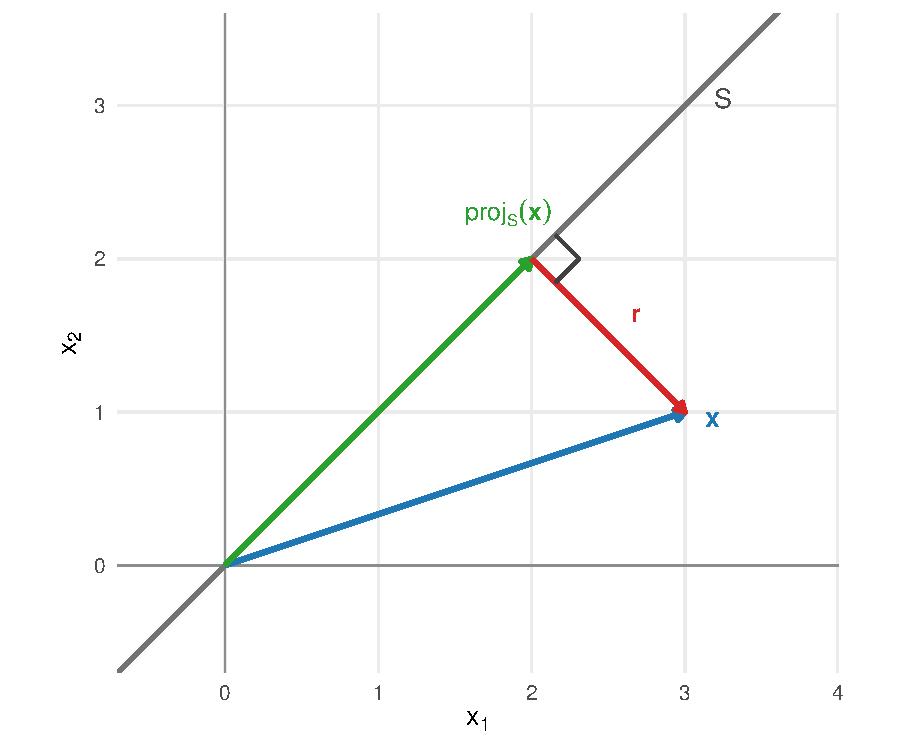
\includegraphics[keepaspectratio]{mod_1_espacos_files/figure-pdf/fig-projecao-ortogonal-1.pdf}}

}

\caption{\label{fig-projecao-ortogonal}Decomposição de um vetor em sua
projeção sobre um subespaço e em um resíduo ortogonal.}

\end{figure}%

A projeção pertence ao subespaço \(S\), enquanto o resíduo pertence a
\(S^{\perp}\). Essa decomposição será estendida para subespaços gerados
por vários vetores.

\subsection{Projeção sobre um subespaço com base
ortonormal}\label{projeuxe7uxe3o-sobre-um-subespauxe7o-com-base-ortonormal}

Considere um subespaço

\[
S
=
\operatorname{span}
\{
\mathbf{q}_1,\ldots,\mathbf{q}_k
\}
\subseteq
\mathbb{R}^p,
\]

em que

\[
\{
\mathbf{q}_1,\ldots,\mathbf{q}_k
\}
\]

é uma base ortonormal de \(S\).

A projeção de \(\mathbf{x}\in\mathbb{R}^p\) sobre \(S\) é obtida somando
as projeções de \(\mathbf{x}\) sobre cada vetor da base:

\[
\operatorname{proj}_{S}(\mathbf{x})
=
\sum_{j=1}^{k}
\left(
\mathbf{q}_j^{\top}\mathbf{x}
\right)
\mathbf{q}_j.
\]

Como

\[
\left(
\mathbf{q}_j^{\top}\mathbf{x}
\right)
\mathbf{q}_j
=
\mathbf{q}_j
\mathbf{q}_j^{\top}
\mathbf{x},
\]

tem-se

\[
\operatorname{proj}_{S}(\mathbf{x})
=
\left(
\sum_{j=1}^{k}
\mathbf{q}_j
\mathbf{q}_j^{\top}
\right)
\mathbf{x}.
\]

Cada matriz

\[
\mathbf{q}_j
\mathbf{q}_j^{\top}
\]

é o produto externo do vetor \(\mathbf{q}_j\) por ele próprio. Como
\(\mathbf{q}_j\neq\mathbf{0}\), cada uma dessas matrizes possui posto
\(1\) e projeta sobre a direção gerada por \(\mathbf{q}_j\).

Reunindo os vetores da base na matriz

\[
\mathbf{Q}
=
\begin{bmatrix}
\mathbf{q}_1
&
\cdots
&
\mathbf{q}_k
\end{bmatrix}
\in
\mathbb{R}^{p\times k},
\]

tem-se

\[
\mathbf{Q}^{\top}\mathbf{Q}
=
\mathbf{I}_k.
\]

Além disso,

\[
\mathbf{Q}\mathbf{Q}^{\top}
=
\sum_{j=1}^{k}
\mathbf{q}_j
\mathbf{q}_j^{\top}.
\]

Portanto,

\[
\operatorname{proj}_{S}(\mathbf{x})
=
\mathbf{Q}
\mathbf{Q}^{\top}
\mathbf{x}.
\]

\begin{proposition}[Projeção sobre uma base
ortonormal]\protect\hypertarget{prp-projecao-base-ortonormal}{}\label{prp-projecao-base-ortonormal}

Se as colunas de

\[\mathbf{Q}\in\mathbb{R}^{p\times k}\]

formam uma base ortonormal de \(S\), então

\[\operatorname{proj}_{S}(\mathbf{x})=\mathbf{Q}\mathbf{Q}^{\top}\mathbf{x}.\]

A matriz de projeção sobre \(S\) é

\[\mathbf{P}_{S}=\mathbf{Q}\mathbf{Q}^{\top}=\sum_{j=1}^{k}\mathbf{q}_j\mathbf{q}_j^{\top}.\]

(Meyer, 2023)

\end{proposition}

O vetor

\[
\mathbf{Q}^{\top}\mathbf{x}
=
\begin{bmatrix}
\mathbf{q}_1^{\top}\mathbf{x}\\
\vdots\\
\mathbf{q}_k^{\top}\mathbf{x}
\end{bmatrix}
\]

contém as coordenadas da projeção de \(\mathbf{x}\) na base ortonormal
de \(S\). A multiplicação por \(\mathbf{Q}\) utiliza essas coordenadas
para reconstruir o vetor projetado no espaço original:

\[
\mathbf{x}
\overset{\mathbf{Q}^{\top}}{\longmapsto}
\mathbf{Q}^{\top}\mathbf{x}
\overset{\mathbf{Q}}{\longmapsto}
\mathbf{Q}\mathbf{Q}^{\top}\mathbf{x}.
\]

Assim, \(\mathbf{Q}^{\top}\) obtém as coordenadas no subespaço, enquanto
\(\mathbf{Q}\) reconstrói o vetor correspondente em \(\mathbb{R}^p\).

\begin{example}[Projeção sobre um
plano]\protect\hypertarget{exm-projecao-base-ortonormal}{}\label{exm-projecao-base-ortonormal}

Considere o subespaço

\[
S
=
\operatorname{span}
\left\{
\begin{bmatrix}
1\\
0\\
0
\end{bmatrix},
\begin{bmatrix}
0\\
1\\
0
\end{bmatrix}
\right\}
\subseteq
\mathbb{R}^3.
\]

Uma base ortonormal de \(S\) é formada por

\[
\mathbf{q}_1
=
\begin{bmatrix}
1\\
0\\
0
\end{bmatrix}
\qquad
\text{e}
\qquad
\mathbf{q}_2
=
\begin{bmatrix}
0\\
1\\
0
\end{bmatrix}.
\]

Assim,

\[
\mathbf{Q}
=
\begin{bmatrix}
1 & 0\\
0 & 1\\
0 & 0
\end{bmatrix}.
\]

A matriz de projeção é

\[
\begin{aligned}
\mathbf{P}_{S}
&=
\mathbf{Q}\mathbf{Q}^{\top}\\
&=
\begin{bmatrix}
1 & 0\\
0 & 1\\
0 & 0
\end{bmatrix}
\begin{bmatrix}
1 & 0 & 0\\
0 & 1 & 0
\end{bmatrix}\\
&=
\begin{bmatrix}
1 & 0 & 0\\
0 & 1 & 0\\
0 & 0 & 0
\end{bmatrix}.
\end{aligned}
\]

Equivalentemente,

\[
\mathbf{P}_{S}
=
\mathbf{q}_1\mathbf{q}_1^{\top}
+
\mathbf{q}_2\mathbf{q}_2^{\top}.
\]

Para

\[
\mathbf{x}
=
\begin{bmatrix}
2\\
-1\\
3
\end{bmatrix},
\]

tem-se

\[
\operatorname{proj}_{S}(\mathbf{x})
=
\mathbf{P}_{S}\mathbf{x}
=
\begin{bmatrix}
2\\
-1\\
0
\end{bmatrix}.
\]

O resíduo é

\[
\mathbf{r}
=
\mathbf{x}
-
\operatorname{proj}_{S}(\mathbf{x})
=
\begin{bmatrix}
0\\
0\\
3
\end{bmatrix},
\]

que pertence a \(S^{\perp}\).

\end{example}

\subsection{Projeção sobre o espaço coluna de uma
matriz}\label{projeuxe7uxe3o-sobre-o-espauxe7o-coluna-de-uma-matriz}

Considere vetores linearmente independentes

\[
\mathbf{a}_1,\ldots,\mathbf{a}_k
\in
\mathbb{R}^p
\]

e a matriz formada por esses vetores:

\[
\mathbf{A}
=
\begin{bmatrix}
\mathbf{a}_1
&
\cdots
&
\mathbf{a}_k
\end{bmatrix}
\in
\mathbb{R}^{p\times k}.
\]

Como os vetores foram previamente nomeados e depois reunidos em
\(\mathbf{A}\), a notação \(\mathbf{a}_1,\ldots,\mathbf{a}_k\) será
mantida nesta subseção.

O subespaço gerado pelas colunas de \(\mathbf{A}\) é

\[
S
=
\mathcal{C}(\mathbf{A})
=
\operatorname{span}
\{
\mathbf{a}_1,\ldots,\mathbf{a}_k
\}.
\]

A projeção de \(\mathbf{x}\in\mathbb{R}^p\) sobre \(S\) deve pertencer
ao espaço coluna de \(\mathbf{A}\). Portanto, possui a forma

\[
\widehat{\mathbf{x}}
=
\mathbf{A}\mathbf{c},
\]

para algum vetor de coeficientes

\[
\mathbf{c}
\in
\mathbb{R}^k.
\]

O resíduo

\[
\mathbf{r}
=
\mathbf{x}
-
\mathbf{A}\mathbf{c}
\]

deve pertencer ao complemento ortogonal de \(\mathcal{C}(\mathbf{A})\).
Assim, ele deve ser ortogonal a todas as colunas de \(\mathbf{A}\):

\[
\mathbf{A}^{\top}
\left(
\mathbf{x}
-
\mathbf{A}\mathbf{c}
\right)
=
\mathbf{0}.
\]

Desenvolvendo,

\[
\mathbf{A}^{\top}\mathbf{x}
-
\mathbf{A}^{\top}\mathbf{A}\mathbf{c}
=
\mathbf{0},
\]

de modo que

\[
\mathbf{A}^{\top}\mathbf{A}\mathbf{c}
=
\mathbf{A}^{\top}\mathbf{x}.
\]

A matriz

\[
\mathbf{A}^{\top}\mathbf{A}
\]

é a matriz de Gram das colunas de \(\mathbf{A}\). Como essas colunas são
linearmente independentes, \(\mathbf{A}^{\top}\mathbf{A}\) é positiva
definida e, portanto, invertível.

Assim,

\[
\mathbf{c}
=
\left(
\mathbf{A}^{\top}\mathbf{A}
\right)^{-1}
\mathbf{A}^{\top}\mathbf{x}.
\]

Substituindo em

\[
\widehat{\mathbf{x}}
=
\mathbf{A}\mathbf{c},
\]

obtém-se

\[
\widehat{\mathbf{x}}
=
\mathbf{A}
\left(
\mathbf{A}^{\top}\mathbf{A}
\right)^{-1}
\mathbf{A}^{\top}
\mathbf{x}.
\]

\begin{proposition}[Projeção sobre o espaço
coluna]\protect\hypertarget{prp-projecao-espaco-coluna}{}\label{prp-projecao-espaco-coluna}

Se

\[\mathbf{A}\in\mathbb{R}^{p\times k}\]

possui colunas linearmente independentes, a projeção ortogonal de
\(\mathbf{x}\in\mathbb{R}^p\) sobre \(\mathcal{C}(\mathbf{A})\) é

\[\operatorname{proj}_{\mathcal{C}(\mathbf{A})}(\mathbf{x})=\mathbf{P}_{\mathbf{A}}\mathbf{x},\]

em que

\[\mathbf{P}_{\mathbf{A}}=\mathbf{A}\left(\mathbf{A}^{\top}\mathbf{A}\right)^{-1}\mathbf{A}^{\top}.\]

\end{proposition}

A matriz \(\mathbf{P}_{\mathbf{A}}\) depende apenas do subespaço gerado
pelas colunas de \(\mathbf{A}\), e não da base particular escolhida para
representá-lo.

De fato, suponha que outra base do mesmo subespaço seja organizada em
uma matriz

\[\mathbf{B}=\mathbf{A}\mathbf{R},\]

em que \(\mathbf{R}\in\mathbb{R}^{k\times k}\) é invertível. Então

\[
\begin{aligned}
\mathbf{P}_{\mathbf{B}}
&=
\mathbf{B}
(\mathbf{B}^{\top}\mathbf{B})^{-1}
\mathbf{B}^{\top}\\
&=
\mathbf{A}\mathbf{R}
\left(
\mathbf{R}^{\top}
\mathbf{A}^{\top}\mathbf{A}
\mathbf{R}
\right)^{-1}
\mathbf{R}^{\top}\mathbf{A}^{\top}\\
&=
\mathbf{A}\mathbf{R}
\mathbf{R}^{-1}
(\mathbf{A}^{\top}\mathbf{A})^{-1}
(\mathbf{R}^{\top})^{-1}
\mathbf{R}^{\top}\mathbf{A}^{\top}\\
&=
\mathbf{A}
(\mathbf{A}^{\top}\mathbf{A})^{-1}
\mathbf{A}^{\top}\\
&=
\mathbf{P}_{\mathbf{A}}.
\end{aligned}
\]

Portanto, bases diferentes do mesmo subespaço produzem a mesma matriz de
projeção ortogonal.

Quando as colunas de \(\mathbf{A}\) são ortonormais,

\[
\mathbf{A}^{\top}\mathbf{A}
=
\mathbf{I}_k,
\]

e a expressão reduz-se a

\[
\mathbf{P}_{\mathbf{A}}
=
\mathbf{A}\mathbf{A}^{\top}.
\]

Esse é exatamente o resultado obtido anteriormente para uma matriz
\(\mathbf{Q}\) cujas colunas formam uma base ortonormal:

\[
\mathbf{P}_{S}
=
\mathbf{Q}\mathbf{Q}^{\top}.
\]

Portanto,

\[
\mathbf{Q}\mathbf{Q}^{\top}
\]

é o caso ortonormal da expressão geral

\[
\mathbf{A}
\left(
\mathbf{A}^{\top}\mathbf{A}
\right)^{-1}
\mathbf{A}^{\top}.
\]

\begin{example}[Projeção utilizando uma base não
ortogonal]\protect\hypertarget{exm-projecao-espaco-coluna}{}\label{exm-projecao-espaco-coluna}

Considere

\[
\mathbf{A}
=
\begin{bmatrix}
1 & 0\\
1 & 1\\
0 & 1
\end{bmatrix}
\]

e

\[
\mathbf{x}
=
\begin{bmatrix}
1\\
2\\
3
\end{bmatrix}.
\]

As colunas de \(\mathbf{A}\) são linearmente independentes. A matriz de
Gram é

\[
\mathbf{A}^{\top}\mathbf{A}
=
\begin{bmatrix}
2 & 1\\
1 & 2
\end{bmatrix},
\]

cuja inversa é

\[
\left(
\mathbf{A}^{\top}\mathbf{A}
\right)^{-1}
=
\frac{1}{3}
\begin{bmatrix}
2 & -1\\
-1 & 2
\end{bmatrix}.
\]

Além disso,

\[
\mathbf{A}^{\top}\mathbf{x}
=
\begin{bmatrix}
3\\
5
\end{bmatrix}.
\]

Os coeficientes da projeção são

\[
\begin{aligned}
\mathbf{c}
&=
\left(
\mathbf{A}^{\top}\mathbf{A}
\right)^{-1}
\mathbf{A}^{\top}\mathbf{x}\\
&=
\frac{1}{3}
\begin{bmatrix}
2 & -1\\
-1 & 2
\end{bmatrix}
\begin{bmatrix}
3\\
5
\end{bmatrix}\\
&=
\frac{1}{3}
\begin{bmatrix}
1\\
7
\end{bmatrix}.
\end{aligned}
\]

Portanto,

\[
\begin{aligned}
\operatorname{proj}_{\mathcal{C}(\mathbf{A})}
(\mathbf{x})
&=
\mathbf{A}\mathbf{c}\\
&=
\begin{bmatrix}
1 & 0\\
1 & 1\\
0 & 1
\end{bmatrix}
\begin{bmatrix}
1/3\\
7/3
\end{bmatrix}\\
&=
\begin{bmatrix}
1/3\\
8/3\\
7/3
\end{bmatrix}.
\end{aligned}
\]

O resíduo é

\[
\mathbf{r}
=
\mathbf{x}
-
\operatorname{proj}_{\mathcal{C}(\mathbf{A})}
(\mathbf{x})
=
\begin{bmatrix}
2/3\\
-2/3\\
2/3
\end{bmatrix}.
\]

A ortogonalidade pode ser verificada por

\[
\mathbf{A}^{\top}\mathbf{r}
=
\begin{bmatrix}
0\\
0
\end{bmatrix}.
\]

Logo,

\[
\mathbf{r}
\in
\mathcal{N}(\mathbf{A}^{\top})
=
\mathcal{C}(\mathbf{A})^{\perp}.
\]

\end{example}

\subsection{Propriedades da matriz de
projeção}\label{propriedades-da-matriz-de-projeuxe7uxe3o}

\begin{proposition}[Propriedades da matriz de
projeção]\protect\hypertarget{prp-propriedades-matriz-projecao}{}\label{prp-propriedades-matriz-projecao}

Se

\[\mathbf{A}\in\mathbb{R}^{p\times k}\]

possui colunas linearmente independentes e

\[\mathbf{P}_{\mathbf{A}}=\mathbf{A}\left(\mathbf{A}^{\top}\mathbf{A}\right)^{-1}\mathbf{A}^{\top},\]

então:

\begin{enumerate}
\def\labelenumi{\arabic{enumi}.}
\item
  \(\mathbf{P}_{\mathbf{A}}\) é simétrica;
\item
  \(\mathbf{P}_{\mathbf{A}}\) é idempotente;
\item
  \(\mathcal{C}(\mathbf{P}_{\mathbf{A}})=\mathcal{C}(\mathbf{A})\);
\item
  \(\mathcal{N}(\mathbf{P}_{\mathbf{A}})=\mathcal{C}(\mathbf{A})^{\perp}=\mathcal{N}(\mathbf{A}^{\top})\);
\item
  \(\operatorname{posto}(\mathbf{P}_{\mathbf{A}})=\operatorname{posto}(\mathbf{A})=k\).
\end{enumerate}

\end{proposition}

\begin{proof}
A simetria decorre de

\[
\begin{aligned}
\mathbf{P}_{\mathbf{A}}^{\top}
&=
\left[
\mathbf{A}
\left(
\mathbf{A}^{\top}\mathbf{A}
\right)^{-1}
\mathbf{A}^{\top}
\right]^{\top}\\
&=
\mathbf{A}
\left[
\left(
\mathbf{A}^{\top}\mathbf{A}
\right)^{-1}
\right]^{\top}
\mathbf{A}^{\top}\\
&=
\mathbf{A}
\left(
\mathbf{A}^{\top}\mathbf{A}
\right)^{-1}
\mathbf{A}^{\top}\\
&=
\mathbf{P}_{\mathbf{A}},
\end{aligned}
\]

pois \(\mathbf{A}^{\top}\mathbf{A}\) e sua inversa são simétricas.

Para verificar a idempotência,

\[
\begin{aligned}
\mathbf{P}_{\mathbf{A}}^2
&=
\mathbf{A}
\left(
\mathbf{A}^{\top}\mathbf{A}
\right)^{-1}
\mathbf{A}^{\top}
\mathbf{A}
\left(
\mathbf{A}^{\top}\mathbf{A}
\right)^{-1}
\mathbf{A}^{\top}\\
&=
\mathbf{A}
\left(
\mathbf{A}^{\top}\mathbf{A}
\right)^{-1}
\mathbf{A}^{\top}\\
&=
\mathbf{P}_{\mathbf{A}}.
\end{aligned}
\]

Para determinar o espaço coluna, observe inicialmente que, para qualquer
\(\mathbf{x}\in\mathbb{R}^p\),

\[
\mathbf{P}_{\mathbf{A}}\mathbf{x}
=
\mathbf{A}
\left[
\left(
\mathbf{A}^{\top}\mathbf{A}
\right)^{-1}
\mathbf{A}^{\top}\mathbf{x}
\right].
\]

Portanto,

\[
\mathbf{P}_{\mathbf{A}}\mathbf{x}
\in
\mathcal{C}(\mathbf{A}),
\]

e, consequentemente,

\[
\mathcal{C}(\mathbf{P}_{\mathbf{A}})
\subseteq
\mathcal{C}(\mathbf{A}).
\]

Reciprocamente, se

\[
\mathbf{y}
\in
\mathcal{C}(\mathbf{A}),
\]

então existe \(\mathbf{c}\in\mathbb{R}^k\) tal que

\[
\mathbf{y}
=
\mathbf{A}\mathbf{c}.
\]

Assim,

\[
\begin{aligned}
\mathbf{P}_{\mathbf{A}}\mathbf{y}
&=
\mathbf{A}
\left(
\mathbf{A}^{\top}\mathbf{A}
\right)^{-1}
\mathbf{A}^{\top}
\mathbf{A}\mathbf{c}\\
&=
\mathbf{A}\mathbf{c}\\
&=
\mathbf{y}.
\end{aligned}
\]

Logo,

\[
\mathcal{C}(\mathbf{A})
\subseteq
\mathcal{C}(\mathbf{P}_{\mathbf{A}}),
\]

e, portanto,

\[
\mathcal{C}(\mathbf{P}_{\mathbf{A}})
=
\mathcal{C}(\mathbf{A}).
\]

Para determinar o espaço nulo, observe que

\[
\begin{aligned}
\mathbf{A}^{\top}\mathbf{P}_{\mathbf{A}}
&=
\mathbf{A}^{\top}
\mathbf{A}
\left(
\mathbf{A}^{\top}\mathbf{A}
\right)^{-1}
\mathbf{A}^{\top}\\
&=
\mathbf{A}^{\top}.
\end{aligned}
\]

Se

\[
\mathbf{x}
\in
\mathcal{N}(\mathbf{P}_{\mathbf{A}}),
\]

então

\[
\mathbf{P}_{\mathbf{A}}\mathbf{x}
=
\mathbf{0},
\]

e, portanto,

\[
\mathbf{A}^{\top}\mathbf{x}
=
\mathbf{A}^{\top}
\mathbf{P}_{\mathbf{A}}\mathbf{x}
=
\mathbf{0}.
\]

Logo,

\[
\mathbf{x}
\in
\mathcal{N}(\mathbf{A}^{\top})
=
\mathcal{C}(\mathbf{A})^{\perp}.
\]

Reciprocamente, se

\[
\mathbf{x}
\in
\mathcal{C}(\mathbf{A})^{\perp},
\]

então

\[
\mathbf{A}^{\top}\mathbf{x}
=
\mathbf{0},
\]

e, consequentemente,

\[
\mathbf{P}_{\mathbf{A}}\mathbf{x}
=
\mathbf{0}.
\]

Assim,

\[
\mathcal{N}(\mathbf{P}_{\mathbf{A}})
=
\mathcal{C}(\mathbf{A})^{\perp}
=
\mathcal{N}(\mathbf{A}^{\top}).
\]

Finalmente, como

\[
\mathcal{C}(\mathbf{P}_{\mathbf{A}})
=
\mathcal{C}(\mathbf{A}),
\]

tem-se

\[
\operatorname{posto}(\mathbf{P}_{\mathbf{A}})
=
\operatorname{posto}(\mathbf{A}).
\]

Como as \(k\) colunas de \(\mathbf{A}\) são linearmente independentes,

\[
\operatorname{posto}(\mathbf{A})
=
k.
\]

Portanto,

\[
\operatorname{posto}(\mathbf{P}_{\mathbf{A}})
=
k.
\]
\end{proof}

A idempotência possui uma interpretação direta: depois que um vetor foi
projetado sobre \(\mathcal{C}(\mathbf{A})\), uma nova aplicação da mesma
projeção não o modifica:

\[
\mathbf{P}_{\mathbf{A}}
\left(
\mathbf{P}_{\mathbf{A}}\mathbf{x}
\right)
=
\mathbf{P}_{\mathbf{A}}\mathbf{x}.
\]

Além disso, a igualdade

\[
\mathcal{N}(\mathbf{P}_{\mathbf{A}})
=
\mathcal{C}(\mathbf{A})^{\perp}
\]

mostra que a projeção anula exatamente a componente de \(\mathbf{x}\)
ortogonal ao subespaço projetado.

\subsection{Aprofundamento: projeção residual e complemento
ortogonal}\label{aprofundamento-projeuxe7uxe3o-residual-e-complemento-ortogonal}

\begin{tcolorbox}[enhanced jigsaw, colback=white, breakable, bottomrule=.15mm, left=2mm, arc=.35mm, rightrule=.15mm, colframe=quarto-callout-note-color-frame, toprule=.15mm, leftrule=.75mm, opacityback=0]

\vspace{-3mm}\textbf{Leitura de aprofundamento}\vspace{3mm}

Esta seção desenvolve a matriz que projeta um vetor sobre o complemento
ortogonal de um subespaço. Essa representação será retomada no estudo de
mínimos quadrados, da Decomposição em Valores Singulares e do modelo
linear multivariado.

\end{tcolorbox}

Considere

\[
\mathbf{A}
\in
\mathbb{R}^{p\times k}
\]

com colunas linearmente independentes e seja

\[
\mathbf{P}_{\mathbf{A}}
\]

a matriz de projeção ortogonal sobre \(\mathcal{C}(\mathbf{A})\).

A componente de \(\mathbf{x}\in\mathbb{R}^p\) que permanece fora desse
subespaço é o resíduo

\[
\mathbf{r}
=
\mathbf{x}
-
\mathbf{P}_{\mathbf{A}}\mathbf{x}.
\]

Definindo

\[
\mathbf{M}_{\mathbf{A}}
=
\mathbf{I}_p
-
\mathbf{P}_{\mathbf{A}},
\]

tem-se

\[
\mathbf{r}
=
\mathbf{M}_{\mathbf{A}}\mathbf{x}.
\]

\begin{definition}[Matriz de projeção
residual]\protect\hypertarget{def-matriz-projecao-residual}{}\label{def-matriz-projecao-residual}

A matriz

\[
\mathbf{M}_{\mathbf{A}}
=
\mathbf{I}_p
-
\mathbf{P}_{\mathbf{A}}
\]

é denominada \textbf{matriz de projeção residual}. Ela realiza a
projeção ortogonal sobre

\[
\mathcal{C}(\mathbf{A})^{\perp}.
\]

Como

\[
\mathcal{C}(\mathbf{A})^{\perp}
=
\mathcal{N}(\mathbf{A}^{\top}),
\]

a matriz \(\mathbf{M}_{\mathbf{A}}\) também pode ser interpretada como a
matriz de projeção ortogonal sobre o espaço nulo à esquerda de
\(\mathbf{A}\).

\end{definition}

A decomposição ortogonal de \(\mathbf{x}\) pode ser escrita como

\[
\mathbf{x}
=
\mathbf{P}_{\mathbf{A}}\mathbf{x}
+
\mathbf{M}_{\mathbf{A}}\mathbf{x},
\]

em que

\[
\mathbf{P}_{\mathbf{A}}\mathbf{x}
\in
\mathcal{C}(\mathbf{A})
\]

e

\[
\mathbf{M}_{\mathbf{A}}\mathbf{x}
\in
\mathcal{N}(\mathbf{A}^{\top})
=
\mathcal{C}(\mathbf{A})^{\perp}.
\]

Como essas duas componentes são ortogonais,

\[
\left(
\mathbf{P}_{\mathbf{A}}\mathbf{x}
\right)^{\top}
\left(
\mathbf{M}_{\mathbf{A}}\mathbf{x}
\right)
=
0.
\]

Consequentemente, pelo Teorema de Pitágoras,

\[
\|\mathbf{x}\|^2
=
\|
\mathbf{P}_{\mathbf{A}}\mathbf{x}
\|^2
+
\|
\mathbf{M}_{\mathbf{A}}\mathbf{x}
\|^2.
\]

\begin{proposition}[Propriedades da matriz de projeção
residual]\protect\hypertarget{prp-propriedades-projecao-residual}{}\label{prp-propriedades-projecao-residual}

Se

\[\mathbf{M}_{\mathbf{A}}=\mathbf{I}_p-\mathbf{P}_{\mathbf{A}},\]

então:

\begin{enumerate}
\def\labelenumi{\arabic{enumi}.}
\item
  \(\mathbf{M}_{\mathbf{A}}\) é simétrica;
\item
  \(\mathbf{M}_{\mathbf{A}}\) é idempotente;
\item
  \(\mathbf{P}_{\mathbf{A}}\mathbf{M}_{\mathbf{A}}=\mathbf{0}\) e
  \(\mathbf{M}_{\mathbf{A}}\mathbf{P}_{\mathbf{A}}=\mathbf{0}\);
\item
  \(\mathcal{C}(\mathbf{M}_{\mathbf{A}})=\mathcal{C}(\mathbf{A})^{\perp}=\mathcal{N}(\mathbf{A}^{\top})\);
\item
  \(\mathcal{N}(\mathbf{M}_{\mathbf{A}})=\mathcal{C}(\mathbf{A})\);
\item
  se \(\mathbf{A}\) possui posto \(k\), então
  \(\operatorname{posto}(\mathbf{M}_{\mathbf{A}})=p-k\).
\end{enumerate}

\end{proposition}

\begin{proof}
Como \(\mathbf{P}_{\mathbf{A}}\) é simétrica,

\[
\begin{aligned}
\mathbf{M}_{\mathbf{A}}^{\top}
&=
\left(
\mathbf{I}_p
-
\mathbf{P}_{\mathbf{A}}
\right)^{\top}\\
&=
\mathbf{I}_p
-
\mathbf{P}_{\mathbf{A}}^{\top}\\
&=
\mathbf{I}_p
-
\mathbf{P}_{\mathbf{A}}\\
&=
\mathbf{M}_{\mathbf{A}}.
\end{aligned}
\]

Portanto, \(\mathbf{M}_{\mathbf{A}}\) é simétrica.

Para verificar a idempotência,

\[
\begin{aligned}
\mathbf{M}_{\mathbf{A}}^2
&=
\left(
\mathbf{I}_p
-
\mathbf{P}_{\mathbf{A}}
\right)^2\\
&=
\mathbf{I}_p
-
2\mathbf{P}_{\mathbf{A}}
+
\mathbf{P}_{\mathbf{A}}^2\\
&=
\mathbf{I}_p
-
\mathbf{P}_{\mathbf{A}}\\
&=
\mathbf{M}_{\mathbf{A}},
\end{aligned}
\]

pois

\[
\mathbf{P}_{\mathbf{A}}^2
=
\mathbf{P}_{\mathbf{A}}.
\]

Além disso,

\[
\begin{aligned}
\mathbf{P}_{\mathbf{A}}
\mathbf{M}_{\mathbf{A}}
&=
\mathbf{P}_{\mathbf{A}}
\left(
\mathbf{I}_p
-
\mathbf{P}_{\mathbf{A}}
\right)\\
&=
\mathbf{P}_{\mathbf{A}}
-
\mathbf{P}_{\mathbf{A}}^2\\
&=
\mathbf{0},
\end{aligned}
\]

e, de forma análoga,

\[
\mathbf{M}_{\mathbf{A}}
\mathbf{P}_{\mathbf{A}}
=
\mathbf{0}.
\]

Para qualquer \(\mathbf{x}\in\mathbb{R}^p\),

\[
\mathbf{P}_{\mathbf{A}}
\mathbf{M}_{\mathbf{A}}
\mathbf{x}
=
\mathbf{0}.
\]

Logo,

\[
\mathbf{M}_{\mathbf{A}}\mathbf{x}
\in
\mathcal{N}(\mathbf{P}_{\mathbf{A}}).
\]

Como

\[
\mathcal{N}(\mathbf{P}_{\mathbf{A}})
=
\mathcal{C}(\mathbf{A})^{\perp},
\]

tem-se

\[
\mathcal{C}(\mathbf{M}_{\mathbf{A}})
\subseteq
\mathcal{C}(\mathbf{A})^{\perp}.
\]

Reciprocamente, se

\[
\mathbf{y}
\in
\mathcal{C}(\mathbf{A})^{\perp},
\]

então

\[
\mathbf{P}_{\mathbf{A}}\mathbf{y}
=
\mathbf{0},
\]

e, portanto,

\[
\begin{aligned}
\mathbf{M}_{\mathbf{A}}\mathbf{y}
&=
\left(
\mathbf{I}_p
-
\mathbf{P}_{\mathbf{A}}
\right)
\mathbf{y}\\
&=
\mathbf{y}.
\end{aligned}
\]

Assim,

\[
\mathcal{C}(\mathbf{A})^{\perp}
\subseteq
\mathcal{C}(\mathbf{M}_{\mathbf{A}}),
\]

e

\[
\mathcal{C}(\mathbf{M}_{\mathbf{A}})
=
\mathcal{C}(\mathbf{A})^{\perp}
=
\mathcal{N}(\mathbf{A}^{\top}).
\]

Agora, se

\[
\mathbf{x}
\in
\mathcal{C}(\mathbf{A}),
\]

então

\[
\mathbf{P}_{\mathbf{A}}\mathbf{x}
=
\mathbf{x}.
\]

Consequentemente,

\[
\mathbf{M}_{\mathbf{A}}\mathbf{x}
=
\mathbf{0},
\]

e

\[
\mathcal{C}(\mathbf{A})
\subseteq
\mathcal{N}(\mathbf{M}_{\mathbf{A}}).
\]

Reciprocamente, se

\[
\mathbf{x}
\in
\mathcal{N}(\mathbf{M}_{\mathbf{A}}),
\]

então

\[
\left(
\mathbf{I}_p
-
\mathbf{P}_{\mathbf{A}}
\right)
\mathbf{x}
=
\mathbf{0},
\]

de modo que

\[
\mathbf{x}
=
\mathbf{P}_{\mathbf{A}}\mathbf{x}.
\]

Como

\[
\mathbf{P}_{\mathbf{A}}\mathbf{x}
\in
\mathcal{C}(\mathbf{A}),
\]

segue que

\[
\mathbf{x}
\in
\mathcal{C}(\mathbf{A}).
\]

Portanto,

\[
\mathcal{N}(\mathbf{M}_{\mathbf{A}})
=
\mathcal{C}(\mathbf{A}).
\]

Finalmente,

\[
\mathcal{C}(\mathbf{M}_{\mathbf{A}})
=
\mathcal{C}(\mathbf{A})^{\perp}.
\]

Como

\[
\dim
\mathcal{C}(\mathbf{A})
=
k,
\]

o teorema da dimensão do complemento ortogonal fornece

\[
\dim
\mathcal{C}(\mathbf{M}_{\mathbf{A}})
=
p-k.
\]

Logo,

\[
\operatorname{posto}
(
\mathbf{M}_{\mathbf{A}}
)
=
p-k.
\]
\end{proof}

\subsection{Projeção como melhor
aproximação}\label{projeuxe7uxe3o-como-melhor-aproximauxe7uxe3o}

A projeção ortogonal pode ser caracterizada por uma propriedade de
otimização: entre todos os vetores de um subespaço, ela é o único vetor
que possui a menor distância até o vetor original.

\begin{theorem}[Teorema da melhor
aproximação]\protect\hypertarget{thm-melhor-aproximacao}{}\label{thm-melhor-aproximacao}

Seja \(S\) um subespaço de \(\mathbb{R}^p\) e seja

\[
\widehat{\mathbf{x}}
=
\operatorname{proj}_{S}(\mathbf{x}).
\]

Então, para qualquer \(\mathbf{y}\in S\),

\[
\|
\mathbf{x}
-
\widehat{\mathbf{x}}
\|
\leq
\|
\mathbf{x}
-
\mathbf{y}
\|.
\]

A igualdade ocorre se, e somente se,

\[
\mathbf{y}
=
\widehat{\mathbf{x}}.
\] (Meyer, 2023)

\end{theorem}

\begin{proof}
Como

\[
\widehat{\mathbf{x}}
\in
S
\]

e

\[
\mathbf{y}
\in
S,
\]

tem-se

\[
\widehat{\mathbf{x}}
-
\mathbf{y}
\in
S.
\]

Por outro lado, como \(\widehat{\mathbf{x}}\) é a projeção ortogonal de
\(\mathbf{x}\) sobre \(S\), o resíduo

\[
\mathbf{x}
-
\widehat{\mathbf{x}}
\]

pertence a \(S^{\perp}\).

Portanto,

\[
\mathbf{x}
-
\widehat{\mathbf{x}}
\]

e

\[
\widehat{\mathbf{x}}
-
\mathbf{y}
\]

são ortogonais.

Escrevendo

\[
\mathbf{x}
-
\mathbf{y}
=
\left(
\mathbf{x}
-
\widehat{\mathbf{x}}
\right)
+
\left(
\widehat{\mathbf{x}}
-
\mathbf{y}
\right),
\]

o Teorema de Pitágoras fornece

\[
\|
\mathbf{x}
-
\mathbf{y}
\|^2
=
\|
\mathbf{x}
-
\widehat{\mathbf{x}}
\|^2
+
\|
\widehat{\mathbf{x}}
-
\mathbf{y}
\|^2.
\]

Como

\[
\|
\widehat{\mathbf{x}}
-
\mathbf{y}
\|^2
\geq
0,
\]

segue que

\[
\|
\mathbf{x}
-
\mathbf{y}
\|^2
\geq
\|
\mathbf{x}
-
\widehat{\mathbf{x}}
\|^2.
\]

A igualdade ocorre se, e somente se,

\[
\|
\widehat{\mathbf{x}}
-
\mathbf{y}
\|^2
=
0,
\]

isto é,

\[
\mathbf{y}
=
\widehat{\mathbf{x}}.
\]
\end{proof}

Portanto, a projeção ortogonal pode ser caracterizada equivalentemente
como

\[\operatorname{proj}_{S}(\mathbf{x})=\underset{\mathbf{y}\in S}{\operatorname{argmin}}\;\|\mathbf{x}-\mathbf{y}\|^2.\]

Assim, projetar ortogonalmente \(\mathbf{x}\) sobre \(S\) equivale a
encontrar, entre todos os vetores pertencentes a \(S\), aquele que está
mais próximo de \(\mathbf{x}\) segundo a distância euclidiana.

Quando \(S=\mathcal{C}(\mathbf{A})\), com
\(\mathbf{A}\in\mathbb{R}^{p\times k}\), todo vetor de \(S\) pode ser
escrito como

\[\mathbf{y}=\mathbf{A}\mathbf{c},\qquad \mathbf{c}\in\mathbb{R}^k.\]

Consequentemente, o problema de melhor aproximação pode ser escrito como

\[\widehat{\mathbf{c}}\in\underset{\mathbf{c}\in\mathbb{R}^k}{\operatorname{argmin}}\;\|\mathbf{x}-\mathbf{A}\mathbf{c}\|^2,\]

e o vetor mais próximo de \(\mathbf{x}\) em \(\mathcal{C}(\mathbf{A})\)
é

\[\widehat{\mathbf{x}}=\mathbf{A}\widehat{\mathbf{c}}=\operatorname{proj}_{\mathcal{C}(\mathbf{A})}(\mathbf{x}).\]

Essa formulação estabelece a ligação entre projeção ortogonal e mínimos
quadrados. O desenvolvimento algébrico dessa relação é apresentado a
seguir como aprofundamento.

\subsection{Aprofundamento: projeções e mínimos
quadrados}\label{aprofundamento-projeuxe7uxf5es-e-muxednimos-quadrados}

\begin{tcolorbox}[enhanced jigsaw, colback=white, breakable, bottomrule=.15mm, left=2mm, arc=.35mm, rightrule=.15mm, colframe=quarto-callout-note-color-frame, toprule=.15mm, leftrule=.75mm, opacityback=0]

\vspace{-3mm}\textbf{Leitura de aprofundamento}\vspace{3mm}

Esta seção desenvolve algebricamente a relação entre projeção ortogonal
e mínimos quadrados. As equações normais, os resíduos, as matrizes de
projeção e a pseudoinversa serão retomados na Decomposição em Valores
Singulares e no modelo linear multivariado.

\end{tcolorbox}

Considere

\[
\mathbf{A}
\in
\mathbb{R}^{n\times k}
\]

e

\[
\mathbf{b}
\in
\mathbb{R}^n.
\]

O sistema

\[
\mathbf{A}\boldsymbol{\beta}
=
\mathbf{b},
\qquad
\boldsymbol{\beta}\in\mathbb{R}^k,
\]

possui solução exata se, e somente se,

\[
\mathbf{b}
\in
\mathcal{C}(\mathbf{A}).
\]

Quando

\[
\mathbf{b}
\notin
\mathcal{C}(\mathbf{A}),
\]

não existe vetor \(\boldsymbol{\beta}\) capaz de reproduzir exatamente
\(\mathbf{b}\). Nesse caso, procura-se a combinação linear das colunas
de \(\mathbf{A}\) que mais se aproxima de \(\mathbf{b}\) no sentido da
distância euclidiana.

O problema de mínimos quadrados é

\[
\widehat{\boldsymbol{\beta}}
\in
\underset{\boldsymbol{\beta}\in\mathbb{R}^k}
{\operatorname{argmin}}
\,
\|
\mathbf{b}
-
\mathbf{A}\boldsymbol{\beta}
\|^2.
\]

Pelo Teorema~\ref{thm-melhor-aproximacao}, o vetor ajustado

\[
\widehat{\mathbf{b}}
=
\mathbf{A}\widehat{\boldsymbol{\beta}}
\]

é a projeção ortogonal de \(\mathbf{b}\) sobre o espaço coluna de
\(\mathbf{A}\):

\[
\widehat{\mathbf{b}}
=
\operatorname{proj}_{\mathcal{C}(\mathbf{A})}
(\mathbf{b}).
\]

O vetor de resíduos é

\[
\widehat{\mathbf{e}}
=
\mathbf{b}
-
\widehat{\mathbf{b}}
=
\mathbf{b}
-
\mathbf{A}\widehat{\boldsymbol{\beta}}.
\]

Como a projeção é ortogonal,

\[
\widehat{\mathbf{e}}
\in
\mathcal{C}(\mathbf{A})^{\perp}.
\]

Pela relação entre os espaços fundamentais,

\[
\mathcal{C}(\mathbf{A})^{\perp}
=
\mathcal{N}(\mathbf{A}^{\top}),
\]

portanto

\[
\widehat{\mathbf{e}}
\in
\mathcal{N}(\mathbf{A}^{\top}).
\]

Consequentemente,

\[
\mathbf{A}^{\top}
\widehat{\mathbf{e}}
=
\mathbf{0}.
\]

Substituindo

\[
\widehat{\mathbf{e}}
=
\mathbf{b}
-
\mathbf{A}\widehat{\boldsymbol{\beta}},
\]

obtém-se

\[
\mathbf{A}^{\top}
\left(
\mathbf{b}
-
\mathbf{A}\widehat{\boldsymbol{\beta}}
\right)
=
\mathbf{0},
\]

e, portanto,

\[
\mathbf{A}^{\top}\mathbf{A}
\widehat{\boldsymbol{\beta}}
=
\mathbf{A}^{\top}\mathbf{b}.
\]

\begin{definition}[Equações
normais]\protect\hypertarget{def-equacoes-normais}{}\label{def-equacoes-normais}

As equações

\[
\mathbf{A}^{\top}\mathbf{A}
\widehat{\boldsymbol{\beta}}
=
\mathbf{A}^{\top}\mathbf{b}
\]

são denominadas \textbf{equações normais} do problema de mínimos
quadrados.

\end{definition}

Se as colunas de \(\mathbf{A}\) são linearmente independentes, então

\[
\operatorname{posto}(\mathbf{A})
=
k
\]

e a matriz de Gram

\[
\mathbf{A}^{\top}\mathbf{A}
\]

é positiva definida e invertível. Nesse caso, as equações normais
possuem solução única:

\[
\widehat{\boldsymbol{\beta}}
=
\left(
\mathbf{A}^{\top}\mathbf{A}
\right)^{-1}
\mathbf{A}^{\top}\mathbf{b}.
\]

O vetor ajustado pode então ser escrito como

\[
\begin{aligned}
\widehat{\mathbf{b}}
&=
\mathbf{A}\widehat{\boldsymbol{\beta}}\\
&=
\mathbf{A}
\left(
\mathbf{A}^{\top}\mathbf{A}
\right)^{-1}
\mathbf{A}^{\top}
\mathbf{b}\\
&=
\mathbf{P}_{\mathbf{A}}\mathbf{b},
\end{aligned}
\]

enquanto o vetor de resíduos é

\[
\begin{aligned}
\widehat{\mathbf{e}}
&=
\mathbf{b}
-
\widehat{\mathbf{b}}\\
&=
\left(
\mathbf{I}_n
-
\mathbf{P}_{\mathbf{A}}
\right)
\mathbf{b}\\
&=
\mathbf{M}_{\mathbf{A}}\mathbf{b}.
\end{aligned}
\]

Aqui,

\[
\mathbf{P}_{\mathbf{A}}
=
\mathbf{A}
\left(
\mathbf{A}^{\top}\mathbf{A}
\right)^{-1}
\mathbf{A}^{\top}
\in
\mathbb{R}^{n\times n}
\]

projeta sobre \(\mathcal{C}(\mathbf{A})\), enquanto

\[
\mathbf{M}_{\mathbf{A}}
=
\mathbf{I}_n
-
\mathbf{P}_{\mathbf{A}}
\in
\mathbb{R}^{n\times n}
\]

projeta sobre

\[
\mathcal{N}(\mathbf{A}^{\top})
=
\mathcal{C}(\mathbf{A})^{\perp}.
\]

\begin{proposition}[Decomposição de mínimos
quadrados]\protect\hypertarget{prp-decomposicao-minimos-quadrados}{}\label{prp-decomposicao-minimos-quadrados}

No problema de mínimos quadrados,

\[\mathbf{b}=\widehat{\mathbf{b}}+\widehat{\mathbf{e}},\]

em que

\[\widehat{\mathbf{b}}\in\mathcal{C}(\mathbf{A})\]

e

\[\widehat{\mathbf{e}}\in\mathcal{N}(\mathbf{A}^{\top})=\mathcal{C}(\mathbf{A})^{\perp}.\]

Consequentemente,

\[\widehat{\mathbf{b}}^{\top}\widehat{\mathbf{e}}=0\]

e

\[\|\mathbf{b}\|^2=\|\widehat{\mathbf{b}}\|^2+\|\widehat{\mathbf{e}}\|^2.\]

(Golub; Van Loan, 2013)

\end{proposition}

Essa decomposição é a aplicação direta da decomposição ortogonal

\[
\mathbb{R}^n
=
\mathcal{C}(\mathbf{A})
\oplus
\mathcal{N}(\mathbf{A}^{\top})
\]

ao vetor \(\mathbf{b}\).

Se as colunas de \(\mathbf{A}\) são linearmente dependentes, o problema
de mínimos quadrados pode possuir diferentes vetores de coeficientes que
produzem o mesmo ajuste. Portanto, \(\widehat{\boldsymbol{\beta}}\) pode
não ser único.

Entretanto, o vetor ajustado

\[
\widehat{\mathbf{b}}
=
\operatorname{proj}_{\mathcal{C}(\mathbf{A})}
(\mathbf{b})
\]

permanece único, pois a projeção depende apenas do subespaço
\(\mathcal{C}(\mathbf{A})\).

Utilizando a pseudoinversa de Moore--Penrose (ver
Definição~\ref{def-pseudoinversa-moore-penrose}),

\[
\widehat{\boldsymbol{\beta}}
=
\mathbf{A}^{+}\mathbf{b}
\]

fornece, entre as soluções de mínimos quadrados, a solução de menor
norma. O vetor ajustado pode ser escrito como

\[
\widehat{\mathbf{b}}
=
\mathbf{A}\mathbf{A}^{+}\mathbf{b},
\]

de modo que

\[
\mathbf{P}_{\mathbf{A}}
=
\mathbf{A}\mathbf{A}^{+}.
\]

A pseudoinversa foi introduzida no capítulo anterior. Sua construção por
meio da Decomposição em Valores Singulares será desenvolvida
posteriormente.

As projeções ponderadas podem ser obtidas substituindo o produto interno
euclidiano por um produto interno induzido por uma matriz positiva
definida. Essa extensão será retomada no estudo de problemas de mínimos
quadrados ponderados.

\section{Síntese do capítulo}\label{suxedntese-do-capuxedtulo-2}

Os espaços vetoriais permitem organizar conjuntos de vetores que
preservam as operações de adição e multiplicação por escalar. Dentro
desses espaços, os subespaços representam estruturas lineares de menor
dimensão, enquanto bases fornecem conjuntos de vetores linearmente
independentes capazes de gerar todo o espaço considerado. Fixada uma
base, cada vetor pode ser representado de maneira única por suas
coordenadas nessa base.

A dimensão quantifica o número de direções independentes necessárias
para representar um espaço. Para uma matriz

\[\mathbf{A}\in\mathbb{R}^{n\times p},\]

essa ideia conduz aos quatro espaços fundamentais:

\[
\mathcal{C}(\mathbf{A}),
\,\,
\mathcal{L}(\mathbf{A}),
\,\,
\mathcal{N}(\mathbf{A})
\,\,\text{e}\,\,
\mathcal{N}(\mathbf{A}^{\top}).
\]

Se \(r=\operatorname{posto}(\mathbf{A})\), suas dimensões são

\[\dim\mathcal{C}(\mathbf{A})=\dim\mathcal{L}(\mathbf{A})=r,\]

\[\dim\mathcal{N}(\mathbf{A})=p-r\]

e

\[\dim\mathcal{N}(\mathbf{A}^{\top})=n-r.\]

Esses espaços se organizam em pares ortogonais:

\[\mathcal{N}(\mathbf{A})=\mathcal{L}(\mathbf{A})^{\perp}\]

e

\[\mathcal{N}(\mathbf{A}^{\top})=\mathcal{C}(\mathbf{A})^{\perp}.\]

Consequentemente,

\[\mathbb{R}^p=\mathcal{L}(\mathbf{A})\oplus\mathcal{N}(\mathbf{A})\]

e

\[\mathbb{R}^n=\mathcal{C}(\mathbf{A})\oplus\mathcal{N}(\mathbf{A}^{\top}).\]

As matrizes de Gram organizam produtos internos entre conjuntos de
vetores. Para uma matriz \(\mathbf{V}\),

\[\mathbf{G}=\mathbf{V}^{\top}\mathbf{V}\]

é simétrica e semidefinida positiva, e sua estrutura permite relacionar
produtos internos, independência linear e posto.

A decomposição ortogonal estabelece que, para qualquer subespaço
\(S\subseteq\mathbb{R}^p\), todo vetor pode ser escrito de maneira única
como

\[\mathbf{x}=\operatorname{proj}_{S}(\mathbf{x})+\mathbf{x}_{S^{\perp}},\]

com \(\operatorname{proj}_{S}(\mathbf{x})\in S\) e
\(\mathbf{x}_{S^{\perp}}\in S^{\perp}\).

Se as colunas de \(\mathbf{Q}\) formam uma base ortonormal de \(S\), a
matriz de projeção é

\[\mathbf{P}_{S}=\mathbf{Q}\mathbf{Q}^{\top}=\sum_{j=1}^{k}\mathbf{q}_j\mathbf{q}_j^{\top}.\]

Se \(S=\mathcal{C}(\mathbf{A})\) e as colunas de \(\mathbf{A}\) são
linearmente independentes, a mesma projeção pode ser escrita como

\[\mathbf{P}_{\mathbf{A}}=\mathbf{A}\left(\mathbf{A}^{\top}\mathbf{A}\right)^{-1}\mathbf{A}^{\top}.\]

A projeção ortogonal possui ainda uma interpretação por otimização:

\[\operatorname{proj}_{S}(\mathbf{x})=\underset{\mathbf{y}\in S}{\operatorname{argmin}}\|\mathbf{x}-\mathbf{y}\|^2.\]

Essa propriedade estabelece a ligação entre geometria, projeções e
problemas de mínimos quadrados.

As partes de aprofundamento generalizam a geometria euclidiana por meio
de produtos internos induzidos por matrizes positivas definidas e
desenvolvem a matriz de projeção residual, as equações normais, o caso
de posto deficiente e a pseudoinversa. Esses resultados serão retomados
quando sua utilização se tornar necessária nos capítulos posteriores.

Ao final deste capítulo, o estudante deverá ser capaz de:

\begin{itemize}
\tightlist
\item
  verificar se um conjunto é um subespaço vetorial;
\item
  interpretar geração, dependência e independência linear;
\item
  identificar bases e determinar dimensões;
\item
  representar vetores por coordenadas em uma base;
\item
  distinguir bases gerais, ortogonais e ortonormais;
\item
  determinar e interpretar os quatro espaços fundamentais de uma matriz;
\item
  relacionar posto, nulidade e dimensão;
\item
  interpretar as relações de ortogonalidade entre os espaços
  fundamentais;
\item
  construir e interpretar matrizes de Gram;
\item
  determinar complementos ortogonais e decomposições ortogonais;
\item
  calcular projeções sobre direções e subespaços;
\item
  interpretar a projeção ortogonal como problema de melhor aproximação;
\item
  reconhecer a relação geométrica entre projeções e mínimos quadrados.
\end{itemize}

No próximo capítulo, as matrizes serão estudadas como representações de
transformações lineares entre espaços vetoriais. Os conceitos de base,
dimensão, posto, espaços fundamentais e projeções desenvolvidos aqui
permitirão interpretar como essas transformações atuam sobre vetores e
subespaços. O espaço nulo e o espaço coluna também serão relacionados,
nesse novo contexto, ao núcleo e à imagem da transformação associada a
uma matriz.

\chapter{Transformações lineares}\label{transformauxe7uxf5es-lineares}

Os capítulos anteriores apresentaram vetores, matrizes, espaços
vetoriais, bases e projeções. Esses objetos permitem representar
observações multivariadas e descrever relações lineares entre suas
coordenadas.

Uma matriz também pode representar uma aplicação que transforma vetores.
Essa aplicação pode alterar a orientação, a escala ou a dimensão da
configuração original. Quando preserva combinações lineares, ela é
denominada \textbf{transformação linear}.

No capítulo anterior, o espaço nulo e o espaço coluna foram definidos
diretamente a partir de uma matriz. Neste capítulo, essas estruturas
serão também interpretadas, respectivamente, como o núcleo e a imagem da
transformação linear associada à matriz.

Este capítulo desenvolve a definição e a representação matricial das
transformações lineares, sua aplicação a matrizes de dados, a composição
de operações, a invertibilidade e a perda de informação. Também são
estudadas transformações geométricas, transformações ortogonais,
mudanças de coordenadas e transformações afins utilizadas no
pré-processamento de dados.

\begin{tcolorbox}[enhanced jigsaw, colback=white, breakable, bottomrule=.15mm, left=2mm, arc=.35mm, rightrule=.15mm, colframe=quarto-callout-note-color-frame, toprule=.15mm, leftrule=.75mm, opacityback=0]

\vspace{-3mm}\textbf{Convenções para transformações lineares}\vspace{3mm}

As convenções vetoriais e matriciais estabelecidas nos capítulos
anteriores permanecem válidas. Neste capítulo, serão utilizadas também
as seguintes convenções:

\begin{itemize}
\tightlist
\item
  \(T:V\to W\) representa uma transformação entre os espaços vetoriais
  \(V\) e \(W\);
\item
  \(V\) representa o domínio e \(W\) o contradomínio da transformação;
\item
  \(\mathbf{x}\in V\) representa um vetor do domínio e
  \(T(\mathbf{x})\in W\) sua imagem pela transformação;
\item
  \(T_{\mathbf{A}}\) representa a transformação linear associada à
  matriz \(\mathbf{A}\);
\item
  \(\mathbf{A}\in\mathbb{R}^{q\times p}\) representa uma transformação
  de \(\mathbb{R}^p\) em \(\mathbb{R}^q\) quando utilizada na forma
  \(T_{\mathbf{A}}(\mathbf{x})=\mathbf{A}\mathbf{x}\);
\item
  \(\ker(T)\) representa o núcleo de uma transformação linear;
\item
  \(\operatorname{Im}(T)\) representa a imagem de uma transformação
  linear;
\item
  \(\mathcal{E}_p\) representa a base canônica de \(\mathbb{R}^p\);
\item
  \([T]_{\mathcal{C}\leftarrow\mathcal{B}}\) representa a matriz de uma
  transformação em relação a uma base \(\mathcal{B}\) do domínio e a uma
  base \(\mathcal{C}\) do contradomínio.
\end{itemize}

As relações entre essas notações e os espaços fundamentais das matrizes
serão estabelecidas ao longo do capítulo.

\end{tcolorbox}

\section{Transformações lineares e representação
matricial}\label{transformauxe7uxf5es-lineares-e-representauxe7uxe3o-matricial}

Uma aplicação entre espaços vetoriais associa a cada vetor do domínio um
vetor do contradomínio. A linearidade exige que essa aplicação preserve
as operações de adição e multiplicação por escalar.

\begin{definition}[Transformação
linear]\protect\hypertarget{def-transformacao-linear}{}\label{def-transformacao-linear}

Sejam \(V\) e \(W\) espaços vetoriais reais. Uma aplicação

\[
T:
V
\longrightarrow
W
\]

é uma \textbf{transformação linear} quando, para quaisquer vetores
\(\mathbf{u},\mathbf{v}\in V\) e escalares
\(\alpha,\beta\in\mathbb{R}\),

\[
T
\left(
\alpha\mathbf{u}
+
\beta\mathbf{v}
\right)
=
\alpha T(\mathbf{u})
+
\beta T(\mathbf{v}).
\]

\end{definition}

Tomando \(\alpha=\beta=1\), obtém-se a preservação da soma:

\[
T(\mathbf{u}+\mathbf{v})
=
T(\mathbf{u})
+
T(\mathbf{v}).
\]

Tomando \(\beta=0\), obtém-se a preservação da multiplicação por
escalar:

\[
T(\alpha\mathbf{u})
=
\alpha T(\mathbf{u}).
\]

Assim, a imagem de uma combinação linear é a combinação linear das
imagens:

\[
T
\left(
\sum_{j=1}^{k}
\alpha_j\mathbf{v}_j
\right)
=
\sum_{j=1}^{k}
\alpha_jT(\mathbf{v}_j).
\]

A Figura~\ref{fig-preservacao-operacoes} representa a preservação da
soma. O paralelogramo formado pelos vetores originais é transformado em
outro paralelogramo cujos lados são as imagens desses vetores.

\begin{figure}

\centering{

\pandocbounded{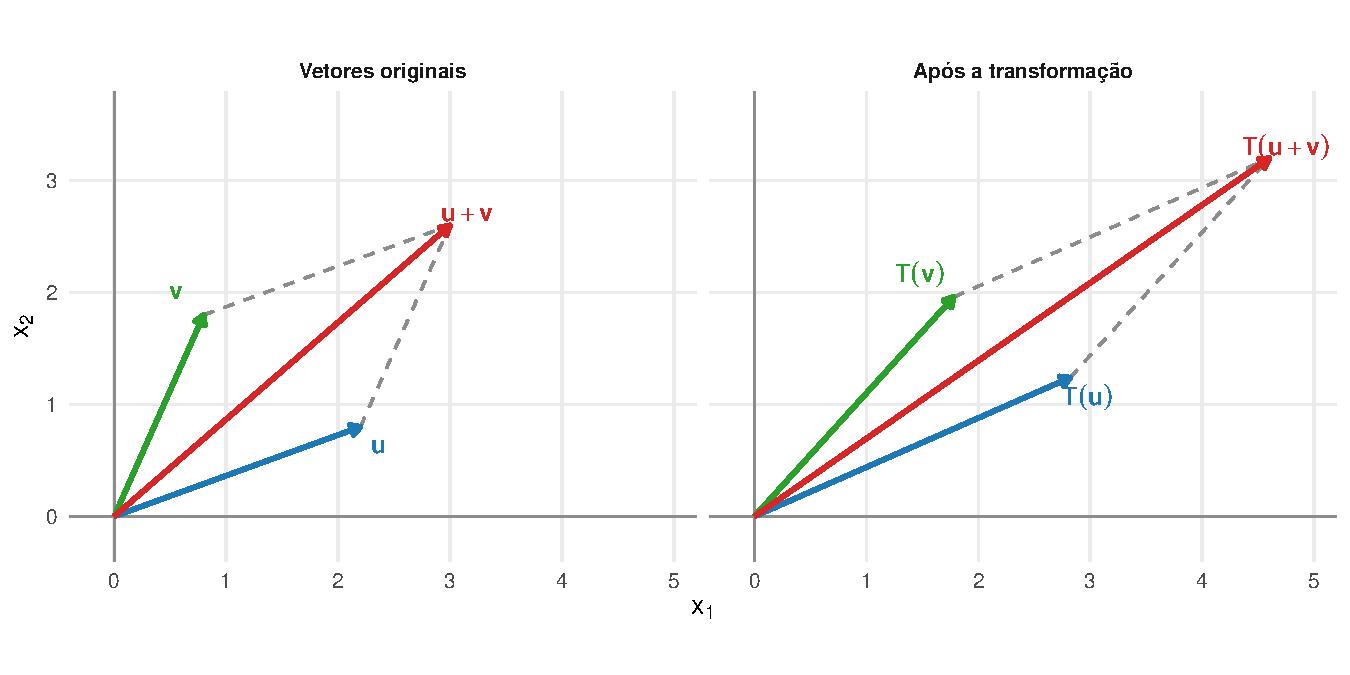
\includegraphics[keepaspectratio]{mod_1_transformacoes_files/figure-pdf/fig-preservacao-operacoes-1.pdf}}

}

\caption{\label{fig-preservacao-operacoes}Preservação da soma de vetores
por uma transformação linear.}

\end{figure}%

No primeiro painel, \(\mathbf{u}+\mathbf{v}\) é a diagonal do
paralelogramo formado pelos vetores originais. No segundo painel, a
relação

\[
T(\mathbf{u}+\mathbf{v})
=
T(\mathbf{u})
+
T(\mathbf{v})
\]

é preservada.

\begin{proposition}[Propriedades elementares das transformações
lineares]\protect\hypertarget{prp-propriedades-elementares-transformacao-linear}{}\label{prp-propriedades-elementares-transformacao-linear}

Se

\[
T:
V
\longrightarrow
W
\]

é uma transformação linear, então:

\begin{enumerate}
\def\labelenumi{\arabic{enumi}.}
\tightlist
\item
  \(T(\mathbf{0})=\mathbf{0}\);
\item
  \(T(-\mathbf{x})=-T(\mathbf{x})\);
\item
  \(T(\mathbf{u}-\mathbf{v}) = T(\mathbf{u})-T(\mathbf{v})\).
\end{enumerate}

(Meyer, 2023)

\end{proposition}

\begin{proof}
Pela homogeneidade,

\[
T(\mathbf{0})
=
T(0\mathbf{x})
=
0T(\mathbf{x})
=
\mathbf{0}.
\]

Também pela homogeneidade,

\[
T(-\mathbf{x})
=
T((-1)\mathbf{x})
=
-T(\mathbf{x}).
\]

Consequentemente,

\[
\begin{aligned}
T(\mathbf{u}-\mathbf{v})
&=
T(\mathbf{u}+(-\mathbf{v}))\\
&=
T(\mathbf{u})
+
T(-\mathbf{v})\\
&=
T(\mathbf{u})
-
T(\mathbf{v}).
\end{aligned}
\]
\end{proof}

A igualdade \(T(\mathbf{0})=\mathbf{0}\) é uma condição necessária para
a linearidade. Se uma aplicação não envia o vetor nulo ao vetor nulo,
ela não é uma transformação linear.

\subsection{Transformação determinada por uma
base}\label{transformauxe7uxe3o-determinada-por-uma-base}

Uma transformação linear é determinada por sua ação sobre os vetores de
uma base do domínio.

\begin{proposition}[Determinação de uma transformação por uma
base]\protect\hypertarget{prp-transformacao-determinada-base}{}\label{prp-transformacao-determinada-base}

Seja \(V\) um espaço vetorial de dimensão finita e seja

\[
\mathcal{B}
=
\{
\mathbf{v}_1,\ldots,\mathbf{v}_k
\}
\]

uma base de \(V\). Uma transformação linear

\[
T:
V
\longrightarrow
W
\]

fica completamente determinada pelos vetores

\[
T(\mathbf{v}_1),\ldots,T(\mathbf{v}_k).
\]

(Meyer, 2023)

\end{proposition}

\begin{proof}
Todo vetor \(\mathbf{x}\in V\) possui uma representação única na base
\(\mathcal{B}\):

\[\mathbf{x}=c_1\mathbf{v}_1+\cdots+c_k\mathbf{v}_k.\]

Pela linearidade,

\[T(\mathbf{x})=c_1T(\mathbf{v}_1)+\cdots+c_kT(\mathbf{v}_k).\]

Portanto, conhecidas as imagens dos vetores da base, a imagem de
qualquer vetor do domínio fica determinada de maneira única.
\end{proof}

\begin{example}[Transformação determinada pelas imagens de uma
base]\protect\hypertarget{exm-transformacao-determinada-base}{}\label{exm-transformacao-determinada-base}

Considere uma transformação

\[
T:
\mathbb{R}^2
\longrightarrow
\mathbb{R}^2
\]

definida sobre os vetores da base canônica por

\[
T(\mathbf{e}_1)
=
\begin{bmatrix}
2\\
1
\end{bmatrix}
\]

e

\[
T(\mathbf{e}_2)
=
\begin{bmatrix}
-1\\
3
\end{bmatrix}.
\]

Para

\[
\mathbf{x}
=
\begin{bmatrix}
x_1\\
x_2
\end{bmatrix}
=
x_1\mathbf{e}_1+x_2\mathbf{e}_2,
\]

tem-se

\[
\begin{aligned}
T(\mathbf{x})
&=
x_1T(\mathbf{e}_1)
+
x_2T(\mathbf{e}_2)\\
&=
x_1
\begin{bmatrix}
2\\
1
\end{bmatrix}
+
x_2
\begin{bmatrix}
-1\\
3
\end{bmatrix}\\
&=
\begin{bmatrix}
2x_1-x_2\\
x_1+3x_2
\end{bmatrix}.
\end{aligned}
\]

Essa expressão pode ser escrita como

\[
T(\mathbf{x})
=
\begin{bmatrix}
2&-1\\
1&3
\end{bmatrix}
\begin{bmatrix}
x_1\\
x_2
\end{bmatrix}.
\]

Portanto, a matriz que representa \(T\) na base canônica é

\[
\mathbf{A}
=
\begin{bmatrix}
2&-1\\
1&3
\end{bmatrix},
\]

cujas colunas são precisamente

\[
T(\mathbf{e}_1)
\qquad
\text{e}
\qquad
T(\mathbf{e}_2).
\]

\end{example}

\subsection{Representação matricial nas bases
canônicas}\label{representauxe7uxe3o-matricial-nas-bases-canuxf4nicas}

Considere uma transformação linear

\[
T:
\mathbb{R}^p
\longrightarrow
\mathbb{R}^q.
\]

Se

\[
\mathcal{E}_p
=
\{
\mathbf{e}_1,\ldots,\mathbf{e}_p
\}
\]

é a base canônica de \(\mathbb{R}^p\), defina

\[
\mathbf{a}_j
=
T(\mathbf{e}_j),
\qquad
j=1,\ldots,p.
\]

Organizando esses vetores nas colunas de uma matriz, obtém-se

\[
\mathbf{A}
=
\begin{bmatrix}
\mathbf{a}_1&
\cdots&
\mathbf{a}_p
\end{bmatrix}
\in
\mathbb{R}^{q\times p}.
\]

Para

\[
\mathbf{x}
=
x_1\mathbf{e}_1
+
\cdots
+
x_p\mathbf{e}_p,
\]

a linearidade fornece

\[
\begin{aligned}
T(\mathbf{x})
&=
x_1T(\mathbf{e}_1)
+
\cdots
+
x_pT(\mathbf{e}_p)\\
&=
x_1\mathbf{a}_1
+
\cdots
+
x_p\mathbf{a}_p\\
&=
\mathbf{A}\mathbf{x}.
\end{aligned}
\]

Isso estabelece a existência de uma matriz que representa \(T\) nas
bases canônicas.

Para verificar a unicidade, suponha que outra matriz

\[
\mathbf{C}
\in
\mathbb{R}^{q\times p}
\]

também satisfaça

\[
T(\mathbf{x})
=
\mathbf{C}\mathbf{x}
\]

para todo \(\mathbf{x}\in\mathbb{R}^p\). Aplicando essa igualdade aos
vetores da base canônica,

\[
\mathbf{C}\mathbf{e}_j
=
T(\mathbf{e}_j)
=
\mathbf{A}\mathbf{e}_j,
\qquad
j=1,\ldots,p.
\]

Como \(\mathbf{A}\mathbf{e}_j\) e \(\mathbf{C}\mathbf{e}_j\)
correspondem, respectivamente, às \(j\)-ésimas colunas de \(\mathbf A\)
e \(\mathbf C\), todas as colunas das duas matrizes são iguais.
Portanto,

\[
\mathbf{C}
=
\mathbf{A}.
\]

A matriz representante de \(T\) nas bases canônicas é, assim, única.

\begin{proposition}[Representação matricial de uma transformação
linear]\protect\hypertarget{prp-representacao-matricial-transformacao}{}\label{prp-representacao-matricial-transformacao}

Toda transformação linear

\[
T:
\mathbb{R}^p
\longrightarrow
\mathbb{R}^q
\]

pode ser representada de maneira única por uma matriz

\[
\mathbf{A}
\in
\mathbb{R}^{q\times p}
\]

tal que

\[
T(\mathbf{x})
=
\mathbf{A}\mathbf{x}
\]

para todo \(\mathbf{x}\in\mathbb{R}^p\).

A \(j\)-ésima coluna de \(\mathbf{A}\) é a imagem do \(j\)-ésimo vetor
da base canônica:

\[\mathbf{a}_j=T(\mathbf{e}_j).\]

(Meyer, 2023)

\end{proposition}

Reciprocamente, toda matriz

\[
\mathbf{A}
\in
\mathbb{R}^{q\times p}
\]

define uma transformação linear

\[
T_{\mathbf{A}}:
\mathbb{R}^p
\longrightarrow
\mathbb{R}^q
\]

por

\[
T_{\mathbf{A}}(\mathbf{x})
=
\mathbf{A}\mathbf{x}.
\]

De fato,

\[
\begin{aligned}
T_{\mathbf{A}}
\left(
\alpha\mathbf{u}
+
\beta\mathbf{v}
\right)
&=
\mathbf{A}
\left(
\alpha\mathbf{u}
+
\beta\mathbf{v}
\right)\\
&=
\alpha\mathbf{A}\mathbf{u}
+
\beta\mathbf{A}\mathbf{v}\\
&=
\alpha T_{\mathbf{A}}(\mathbf{u})
+
\beta T_{\mathbf{A}}(\mathbf{v}).
\end{aligned}
\]

A matriz apresentada nessa representação corresponde às bases canônicas
do domínio e do contradomínio. A representação em bases gerais será
desenvolvida posteriormente.

\subsection{Núcleo e imagem de uma transformação
linear}\label{nuxfacleo-e-imagem-de-uma-transformauxe7uxe3o-linear}

Dois subespaços descrevem aspectos fundamentais da ação de uma
transformação linear: os vetores do domínio que são enviados ao vetor
nulo e os vetores do contradomínio que podem ser obtidos pela
transformação.

\begin{definition}[Núcleo e imagem de uma transformação
linear]\protect\hypertarget{def-nucleo-imagem-transformacao}{}\label{def-nucleo-imagem-transformacao}

Seja

\[T:V\longrightarrow W\]

uma transformação linear.

O \textbf{núcleo} de \(T\) é o conjunto

\[
\ker(T)
=
\{
\mathbf{x}\in V:T(\mathbf{x})=\mathbf{0}
\}.
\]

A \textbf{imagem} de \(T\) é o conjunto

\[
\operatorname{Im}(T)
=
\{
T(\mathbf{x}):\mathbf{x}\in V
\}.
\]

O núcleo é um subespaço do domínio \(V\), enquanto a imagem é um
subespaço do contradomínio \(W\).

\end{definition}

Para a transformação matricial

\[
T_{\mathbf A}(\mathbf{x})
=
\mathbf A\mathbf{x},
\]

o núcleo é

\[
\begin{aligned}
\ker(T_{\mathbf A})
&=
\left\{
\mathbf{x}\in\mathbb R^p:
\mathbf A\mathbf{x}=\mathbf 0
\right\}\\
&=
\mathcal N(\mathbf A),
\end{aligned}
\]

e a imagem é

\[
\begin{aligned}
\operatorname{Im}(T_{\mathbf A})
&=
\left\{
\mathbf A\mathbf{x}:
\mathbf{x}\in\mathbb R^p
\right\}\\
&=
\mathcal C(\mathbf A).
\end{aligned}
\]

\begin{tcolorbox}[enhanced jigsaw, colback=white, breakable, bottomrule=.15mm, left=2mm, arc=.35mm, rightrule=.15mm, colframe=quarto-callout-note-color-frame, toprule=.15mm, leftrule=.75mm, opacityback=0]

\vspace{-3mm}\textbf{Relação com os subespaços associados a uma matriz}\vspace{3mm}

O \textbf{espaço nulo} e o \textbf{espaço coluna} estudados no capítulo
anterior correspondem, respectivamente, ao \textbf{núcleo} e à
\textbf{imagem} da transformação linear associada à matriz
\(\mathbf A\):

\[
\mathcal N(\mathbf A)
=
\ker(T_{\mathbf A}),
\qquad
\mathcal C(\mathbf A)
=
\operatorname{Im}(T_{\mathbf A}).
\]

Se

\[
T_{\mathbf A}:
\mathbb R^p
\longrightarrow
\mathbb R^q,
\]

o \textbf{contradomínio} é \(\mathbb R^q\), enquanto a imagem é o
subespaço efetivamente alcançado pela transformação,

\[
\operatorname{Im}(T_{\mathbf A})
\subseteq
\mathbb R^q.
\]

\end{tcolorbox}

\subsection{Imagem de um subespaço}\label{imagem-de-um-subespauxe7o}

Considere um subespaço

\[
S
=
\operatorname{span}
\{
\mathbf{v}_1,\ldots,\mathbf{v}_k
\}
\subseteq
V.
\]

Todo vetor \(\mathbf{x}\in S\) possui a forma

\[
\mathbf{x}
=
\alpha_1\mathbf{v}_1
+
\cdots
+
\alpha_k\mathbf{v}_k.
\]

Aplicando \(T\),

\[
T(\mathbf{x})
=
\alpha_1T(\mathbf{v}_1)
+
\cdots
+
\alpha_kT(\mathbf{v}_k).
\]

Portanto,

\[
T(S)
=
\operatorname{span}
\{
T(\mathbf{v}_1),\ldots,T(\mathbf{v}_k)
\}.
\]

A imagem de um subespaço por uma transformação linear também é um
subespaço do contradomínio.

A transformação preserva as combinações lineares, mas pode reduzir a
dimensão do espaço gerado. Considere

\[
\mathbf{A}
=
\begin{bmatrix}
1&0\\
0&0
\end{bmatrix}.
\]

Os vetores canônicos \(\mathbf{e}_1\) e \(\mathbf{e}_2\) são linearmente
independentes, mas

\[
\mathbf{A}\mathbf{e}_1
=
\begin{bmatrix}
1\\
0
\end{bmatrix}
\]

e

\[
\mathbf{A}\mathbf{e}_2
=
\begin{bmatrix}
0\\
0
\end{bmatrix}.
\]

A segunda direção é eliminada e a imagem da transformação possui
dimensão 1. A relação entre preservação da independência linear, núcleo,
posto e injetividade será desenvolvida na seção sobre invertibilidade e
perda de informação.

\section{Transformação de vetores e matrizes de
dados}\label{transformauxe7uxe3o-de-vetores-e-matrizes-de-dados}

A representação

\[
T(\mathbf{x})
=
\mathbf{A}\mathbf{x}
\]

considera cada observação como um vetor-coluna. Em uma matriz de dados,
as observações são organizadas nas linhas. A aplicação simultânea da
transformação exige, portanto, a transposição da matriz que atua sobre
cada vetor.

Considere

\[
\mathbf{X}
=
\begin{bmatrix}
\mathbf{x}_1^{\top}\\
\mathbf{x}_2^{\top}\\
\vdots\\
\mathbf{x}_n^{\top}
\end{bmatrix}
\in
\mathbb{R}^{n\times p},
\]

em que

\[
\mathbf{x}_i
\in
\mathbb{R}^p,
\qquad
i=1,\ldots,n,
\]

representa a \(i\)-ésima observação.

Se

\[
T:
\mathbb{R}^p
\longrightarrow
\mathbb{R}^q
\]

é representada por

\[
\mathbf{A}
\in
\mathbb{R}^{q\times p},
\]

a imagem de cada observação é

\[
\mathbf{y}_i
=
\mathbf{A}\mathbf{x}_i
\in
\mathbb{R}^q.
\]

Transpondo essa igualdade,

\[
\mathbf{y}_i^{\top}
=
\mathbf{x}_i^{\top}\mathbf{A}^{\top}.
\]

\begin{proposition}[Transformação de uma matriz de
dados]\protect\hypertarget{prp-transformacao-matriz-dados}{}\label{prp-transformacao-matriz-dados}

Se as observações estão organizadas nas linhas de

\[
\mathbf{X}
\in
\mathbb{R}^{n\times p}
\]

e cada observação é transformada por

\[
\mathbf{y}_i
=
\mathbf{A}\mathbf{x}_i,
\qquad
\mathbf{A}
\in
\mathbb{R}^{q\times p},
\]

então a matriz transformada é

\[
\mathbf{Y}
=
\mathbf{X}\mathbf{A}^{\top}
\in
\mathbb{R}^{n\times q}.
\]

\end{proposition}

\begin{proof}
A \(i\)-ésima linha de \(\mathbf{Y}\) é

\[
\mathbf{x}_i^{\top}\mathbf{A}^{\top}.
\]

Como

\[
\mathbf{x}_i^{\top}\mathbf{A}^{\top}
=
\left(
\mathbf{A}\mathbf{x}_i
\right)^{\top}
=
\mathbf{y}_i^{\top},
\]

tem-se

\[
\mathbf{Y}
=
\begin{bmatrix}
\mathbf{y}_1^{\top}\\
\mathbf{y}_2^{\top}\\
\vdots\\
\mathbf{y}_n^{\top}
\end{bmatrix}
=
\mathbf{X}\mathbf{A}^{\top}.
\]
\end{proof}

As dimensões da multiplicação são

\[
\underbrace{\mathbf{X}}_{n\times p}
\underbrace{\mathbf{A}^{\top}}_{p\times q}
=
\underbrace{\mathbf{Y}}_{n\times q}.
\]

A transposição não altera a transformação definida sobre vetores-coluna.
Ela adapta a multiplicação à organização das observações nas linhas da
matriz de dados.

\subsection{Novas variáveis como combinações
lineares}\label{novas-variuxe1veis-como-combinauxe7uxf5es-lineares}

Seja

\[
\mathbf{w}_j
\in
\mathbb{R}^p
\]

o vetor de coeficientes associado à \(j\)-ésima coordenada transformada.
As linhas de \(\mathbf{A}\) podem ser representadas por

\[
\mathbf{A}
=
\begin{bmatrix}
\mathbf{w}_1^{\top}\\
\mathbf{w}_2^{\top}\\
\vdots\\
\mathbf{w}_q^{\top}
\end{bmatrix},
\]

de modo que

\[
\mathbf{A}^{\top}
=
\begin{bmatrix}
\mathbf{w}_1&
\mathbf{w}_2&
\cdots&
\mathbf{w}_q
\end{bmatrix}.
\]

Consequentemente,

\[
\mathbf{Y}
=
\begin{bmatrix}
\mathbf{X}\mathbf{w}_1&
\mathbf{X}\mathbf{w}_2&
\cdots&
\mathbf{X}\mathbf{w}_q
\end{bmatrix}.
\]

A \(j\)-ésima coluna da matriz transformada é

\[\mathbf{y}_{\cdot j}=\mathbf{X}\mathbf{w}_j.\]

Cada nova variável é, portanto, uma combinação linear das variáveis
originais. Para a \(i\)-ésima observação,

\[
y_{ij}
=
a_{j1}x_{i1}
+
a_{j2}x_{i2}
+
\cdots
+
a_{jp}x_{ip}.
\]

Essa relação permite interpretar a transformação de duas maneiras
complementares:

\begin{itemize}
\tightlist
\item
  cada linha de \(\mathbf{Y}\) é a imagem de uma observação;
\item
  cada coluna de \(\mathbf{Y}\) é uma nova variável construída por
  combinação linear.
\end{itemize}

\begin{example}[Transformação de um conjunto de
observações]\protect\hypertarget{exm-transformacao-matriz-dados}{}\label{exm-transformacao-matriz-dados}

Considere

\[
\mathbf{X}
=
\begin{bmatrix}
1&2\\
3&1\\
2&4
\end{bmatrix}
\]

e

\[
\mathbf{A}
=
\begin{bmatrix}
1&1\\
2&-1
\end{bmatrix}.
\]

Para uma observação genérica,

\[
\mathbf{x}_i
=
\begin{bmatrix}
x_{i1}\\
x_{i2}
\end{bmatrix},
\]

tem-se

\[
\begin{aligned}
\mathbf{y}_i
&=
\mathbf{A}\mathbf{x}_i\\
&=
\begin{bmatrix}
1&1\\
2&-1
\end{bmatrix}
\begin{bmatrix}
x_{i1}\\
x_{i2}
\end{bmatrix}\\
&=
\begin{bmatrix}
x_{i1}+x_{i2}\\
2x_{i1}-x_{i2}
\end{bmatrix}.
\end{aligned}
\]

Como as observações estão nas linhas de \(\mathbf{X}\),

\[
\begin{aligned}
\mathbf{Y}
&=
\mathbf{X}\mathbf{A}^{\top}\\
&=
\begin{bmatrix}
1&2\\
3&1\\
2&4
\end{bmatrix}
\begin{bmatrix}
1&2\\
1&-1
\end{bmatrix}\\
&=
\begin{bmatrix}
3&0\\
4&5\\
6&0
\end{bmatrix}.
\end{aligned}
\]

A primeira variável transformada é a soma das duas variáveis originais:

\[\mathbf{y}_{\cdot 1}=\mathbf{x}_{\cdot 1}+\mathbf{x}_{\cdot 2}.\]

A segunda é

\[\mathbf{y}_{\cdot 2}=2\mathbf{x}_{\cdot 1}-\mathbf{x}_{\cdot 2}.\]

\end{example}

\subsection{Dimensão da configuração
transformada}\label{dimensuxe3o-da-configurauxe7uxe3o-transformada}

Quando

\[
q=p,
\]

a transformação atua entre espaços de mesma dimensão:

\[
T:
\mathbb{R}^p
\longrightarrow
\mathbb{R}^p.
\]

e o domínio e o contradomínio possuem a mesma dimensão. A dimensão
efetiva da imagem, entretanto, pode ser menor que \(p\) quando
\(\mathbf{A}\) não possui posto completo.

Quando

\[
q<p,
\]

a transformação produz vetores com menos coordenadas:

\[
T:
\mathbb{R}^p
\longrightarrow
\mathbb{R}^q.
\]

Quando

\[
q>p,
\]

os vetores passam a ser representados em um espaço com mais coordenadas.
Esse aumento do contradomínio não implica aumento da dimensão efetiva da
imagem.

Se

\[
\operatorname{posto}(\mathbf{A})
=
r,
\]

então

\[
\mathcal{C}(\mathbf{A})
\subseteq
\mathbb{R}^q
\]

possui dimensão \(r\). Como

\[
\mathbf{y}_i
=
\mathbf{A}\mathbf{x}_i,
\]

todas as observações transformadas pertencem a esse espaço:

\[
\mathbf{y}_i
\in
\mathcal{C}(\mathbf{A}).
\]

Portanto, todas as observações transformadas pertencem a um subespaço de
dimensão

\[r=\operatorname{posto}(\mathbf{A}).\]

Assim, a dimensão da configuração transformada não pode exceder
\(\operatorname{posto}(\mathbf{A})\), embora possa ser menor, dependendo
da configuração original dos dados.

Se

\[
r=q,
\]

a imagem coincide com todo o contradomínio.

Se

\[
r<q,
\]

a imagem ocupa apenas um subespaço próprio de \(\mathbb{R}^q\).

Quando \(r<p\), a transformação possui núcleo não trivial e elimina pelo
menos uma direção do domínio. Existe, nesse caso, um vetor não nulo

\[\mathbf{v}\in\ker(T_{\mathbf{A}})=\mathcal{N}(\mathbf{A})\]

tal que

\[
\mathbf{A}\mathbf{v}
=
\mathbf{0}.
\]

Para qualquer \(\mathbf{x}\in\mathbb{R}^p\),

\[
\begin{aligned}
\mathbf{A}
\left(
\mathbf{x}+\mathbf{v}
\right)
&=
\mathbf{A}\mathbf{x}
+
\mathbf{A}\mathbf{v}\\
&=
\mathbf{A}\mathbf{x}.
\end{aligned}
\]

Vetores distintos podem, portanto, produzir a mesma imagem quando
diferem por um elemento do espaço nulo.

A Figura~\ref{fig-efeitos-transformacoes} compara os efeitos de
diferentes matrizes sobre uma mesma configuração de pontos.

\begin{figure}

\centering{

\pandocbounded{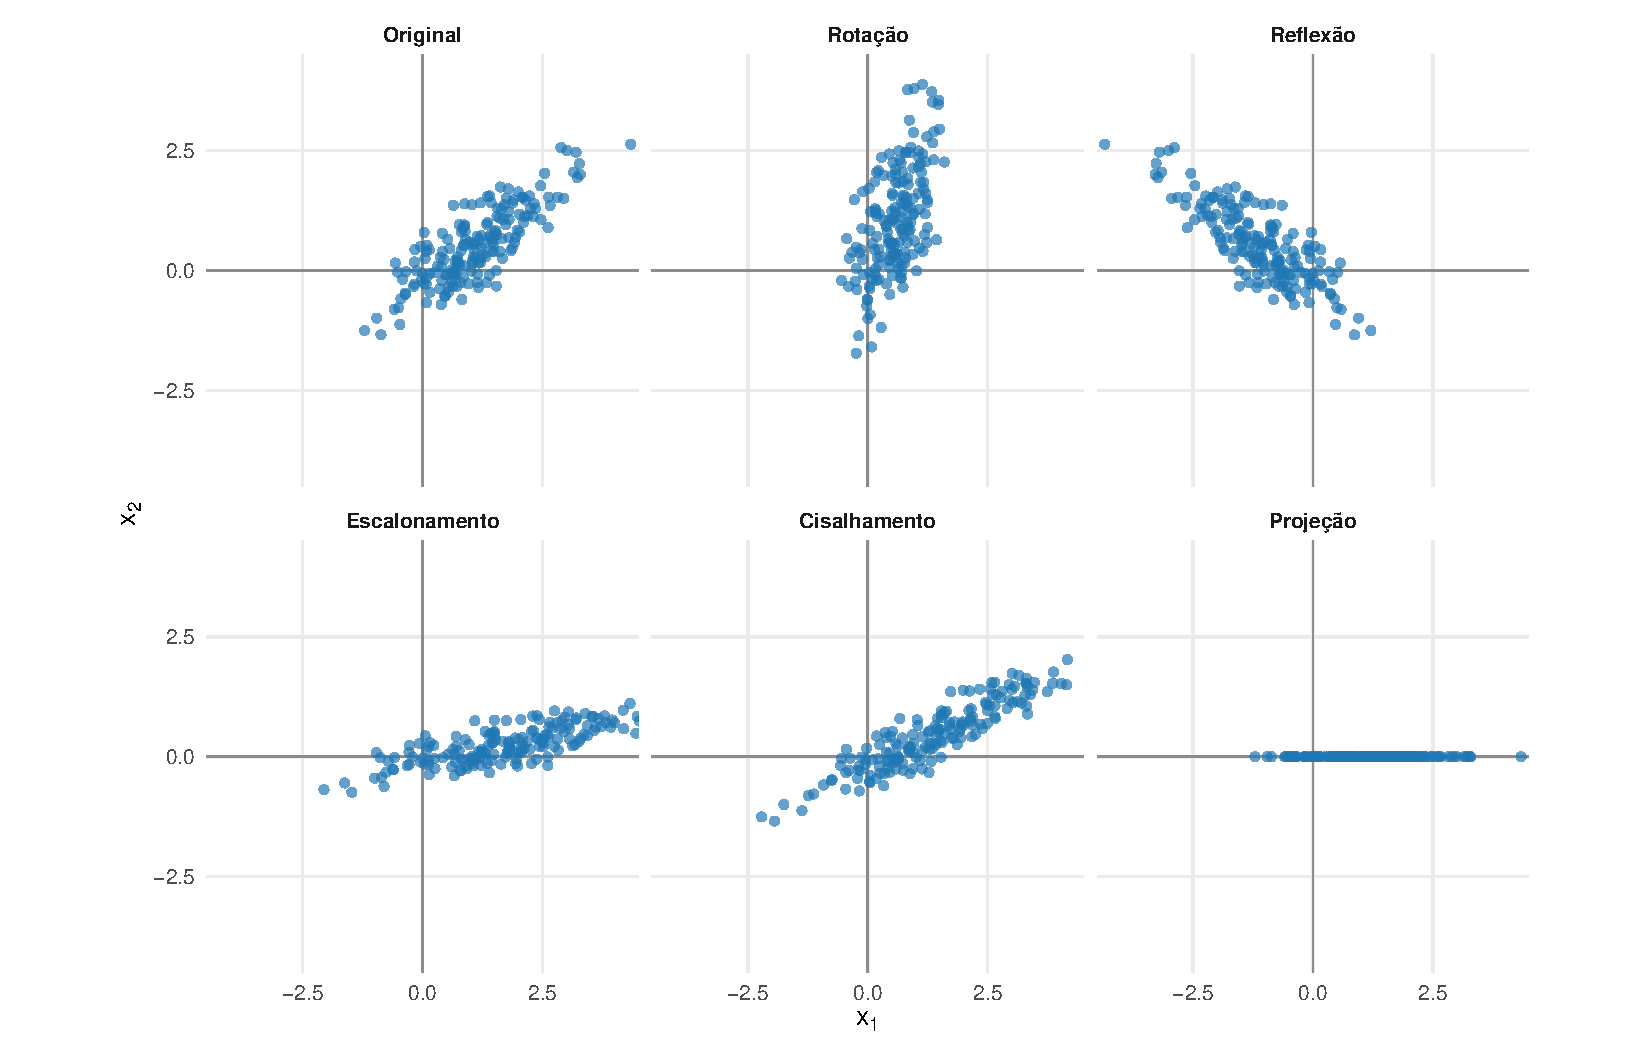
\includegraphics[keepaspectratio]{mod_1_transformacoes_files/figure-pdf/fig-efeitos-transformacoes-1.pdf}}

}

\caption{\label{fig-efeitos-transformacoes}Efeito de diferentes
transformações lineares sobre uma mesma configuração de pontos.}

\end{figure}%

A rotação gira a configuração em relação aos eixos coordenados sem
alterar sua forma. A reflexão também preserva a forma, mas inverte sua
orientação. O escalonamento modifica os comprimentos em cada direção,
enquanto o cisalhamento altera uma coordenada de acordo com a outra. A
projeção elimina a segunda coordenada e reduz a configuração a uma reta.

As cinco operações preservam combinações lineares. Entretanto, não
preservam necessariamente comprimentos, ângulos, áreas ou dimensão.

\subsection{Efeito sobre diferenças e produtos
internos}\label{efeito-sobre-diferenuxe7as-e-produtos-internos}

Se duas observações são representadas por \(\mathbf{x}_i\) e
\(\mathbf{x}_j\), então

\[
\begin{aligned}
\mathbf{y}_i-\mathbf{y}_j
&=
\mathbf{A}\mathbf{x}_i
-
\mathbf{A}\mathbf{x}_j\\
&=
\mathbf{A}
\left(
\mathbf{x}_i-\mathbf{x}_j
\right).
\end{aligned}
\]

A transformação das diferenças determina o efeito sobre as distâncias. O
quadrado da distância entre as imagens é

\[
\begin{aligned}
\|
\mathbf{y}_i-\mathbf{y}_j
\|^2
&=
\left[
\mathbf{A}
\left(
\mathbf{x}_i-\mathbf{x}_j
\right)
\right]^{\top}
\left[
\mathbf{A}
\left(
\mathbf{x}_i-\mathbf{x}_j
\right)
\right]\\
&=
\left(
\mathbf{x}_i-\mathbf{x}_j
\right)^{\top}
\mathbf{A}^{\top}\mathbf{A}
\left(
\mathbf{x}_i-\mathbf{x}_j
\right).
\end{aligned}
\]

A matriz

\[\mathbf{A}^{\top}\mathbf{A}\]

descreve, no domínio, como a transformação modifica produtos internos,
comprimentos e distâncias. Quando \(\mathbf{A}\) possui posto completo
nas colunas, \(\mathbf{A}^{\top}\mathbf{A}\) é positiva definida e
determina um produto interno no domínio. Quando \(\mathbf{A}\) não
possui posto completo nas colunas, essa matriz é apenas semidefinida
positiva e algumas direções são eliminadas pela transformação.

Para quaisquer vetores \(\mathbf{x},\mathbf{z}\in\mathbb{R}^p\),

\[
\begin{aligned}
T(\mathbf{x})^{\top}T(\mathbf{z})
&=
(\mathbf{A}\mathbf{x})^{\top}
(\mathbf{A}\mathbf{z})\\
&=
\mathbf{x}^{\top}
\mathbf{A}^{\top}\mathbf{A}
\mathbf{z}.
\end{aligned}
\]

Em particular,

\[
\|
\mathbf{A}\mathbf{x}
\|^2
=
\mathbf{x}^{\top}
\mathbf{A}^{\top}\mathbf{A}
\mathbf{x}.
\]

Como

\[
\mathbf{x}^{\top}
\mathbf{A}^{\top}\mathbf{A}
\mathbf{x}
=
\|
\mathbf{A}\mathbf{x}
\|^2
\geq
0,
\]

a matriz \(\mathbf{A}^{\top}\mathbf{A}\) é simétrica e semidefinida
positiva.

Se \(\mathbf{A}\) possui posto completo nas colunas, então

\[
\mathcal{N}(\mathbf{A})
=
\{\mathbf{0}\}
\]

e

\[
\mathbf{x}^{\top}
\mathbf{A}^{\top}\mathbf{A}
\mathbf{x}
>
0
\]

para todo \(\mathbf{x}\neq\mathbf{0}\). Nesse caso,

\[
\mathbf{A}^{\top}\mathbf{A}
\succ
0,
\]

e a expressão

\[
\|\mathbf{x}\|_{\mathbf{A}^{\top}\mathbf{A}}
=
\sqrt{
\mathbf{x}^{\top}
\mathbf{A}^{\top}\mathbf{A}
\mathbf{x}
}
=
\|\mathbf{A}\mathbf{x}\|
\]

define uma norma em \(\mathbb{R}^p\).

Quando \(\mathbf{A}\) não possui posto completo nas colunas, existem
vetores não nulos em

\[\ker(T_{\mathbf{A}})=\mathcal{N}(\mathbf{A})\]

para os quais

\[\|\mathbf{x}\|_{\mathbf{A}^{\top}\mathbf{A}}=0.\]

Nesse caso, \(\|\cdot\|_{\mathbf{A}^{\top}\mathbf{A}}\) define uma
seminorma.

\subsection{Transformação das matrizes de produtos
internos}\label{transformauxe7uxe3o-das-matrizes-de-produtos-internos}

A matriz de Gram entre as observações originais é

\[
\mathbf{G}_{\mathbf{X}}
=
\mathbf{X}\mathbf{X}^{\top}.
\]

Para

\[
\mathbf{Y}
=
\mathbf{X}\mathbf{A}^{\top},
\]

tem-se

\[
\begin{aligned}
\mathbf{G}_{\mathbf{Y}}
&=
\mathbf{Y}\mathbf{Y}^{\top}\\
&=
\mathbf{X}
\mathbf{A}^{\top}
\mathbf{A}
\mathbf{X}^{\top}.
\end{aligned}
\]

Portanto,

\[
\mathbf{G}_{\mathbf{Y}}
=
\mathbf{X}
\mathbf{A}^{\top}
\mathbf{A}
\mathbf{X}^{\top}.
\]

Se

\[
\mathbf{A}^{\top}\mathbf{A}
=
\mathbf{I}_p,
\]

então

\[
\mathbf{G}_{\mathbf{Y}}
=
\mathbf{X}\mathbf{X}^{\top}
=
\mathbf{G}_{\mathbf{X}}.
\]

Nesse caso, todos os produtos internos entre as observações são
preservados.

A matriz de produtos cruzados entre as variáveis transformadas é

\[
\begin{aligned}
\mathbf{Y}^{\top}\mathbf{Y}
&=
\left(
\mathbf{X}\mathbf{A}^{\top}
\right)^{\top}
\left(
\mathbf{X}\mathbf{A}^{\top}
\right)\\
&=
\mathbf{A}
\mathbf{X}^{\top}\mathbf{X}
\mathbf{A}^{\top}.
\end{aligned}
\]

Logo,

\[
\mathbf{Y}^{\top}\mathbf{Y}
=
\mathbf{A}
\mathbf{X}^{\top}\mathbf{X}
\mathbf{A}^{\top}.
\]

Essa expressão descreve como os produtos cruzados entre as novas
variáveis são obtidos a partir dos produtos cruzados entre as variáveis
originais.

Quando \(\mathbf{X}\) está centralizada, a mesma estrutura permite
descrever posteriormente a transformação da matriz de covariâncias. Por
enquanto, a relação mostra que uma transformação linear modifica
simultaneamente a geometria das observações e as relações entre as
variáveis.

\section{Composição, invertibilidade e perda de
informação}\label{composiuxe7uxe3o-invertibilidade-e-perda-de-informauxe7uxe3o}

Transformações lineares podem ser aplicadas sucessivamente. A matriz da
transformação resultante é obtida pelo produto das matrizes que
representam cada etapa.

\subsection{Composição de transformações
lineares}\label{composiuxe7uxe3o-de-transformauxe7uxf5es-lineares}

Considere

\[
T_1:
\mathbb{R}^p
\longrightarrow
\mathbb{R}^q
\]

e

\[
T_2:
\mathbb{R}^q
\longrightarrow
\mathbb{R}^r,
\]

representadas, respectivamente, por

\[
\mathbf{A}
\in
\mathbb{R}^{q\times p}
\]

e

\[
\mathbf{B}
\in
\mathbb{R}^{r\times q}.
\]

Para \(\mathbf{x}\in\mathbb{R}^p\),

\[
T_1(\mathbf{x})
=
\mathbf{A}\mathbf{x}.
\]

Aplicando \(T_2\) à imagem produzida por \(T_1\),

\[
\begin{aligned}
T_2
\left(
T_1(\mathbf{x})
\right)
&=
\mathbf{B}
\left(
\mathbf{A}\mathbf{x}
\right)\\
&=
\left(
\mathbf{B}\mathbf{A}
\right)
\mathbf{x}.
\end{aligned}
\]

\begin{proposition}[Matriz de uma
composição]\protect\hypertarget{prp-matriz-composicao}{}\label{prp-matriz-composicao}

Se \(T_1\) é representada por \(\mathbf{A}\) e \(T_2\) é representada
por \(\mathbf{B}\), então a composição

\[
T_2\circ T_1
\]

é representada por

\[
\mathbf{B}\mathbf{A}.
\]

Em particular,

\[
[T_2\circ T_1]
=
[T_2][T_1].
\]

\end{proposition}

A ordem do produto é interpretada da direita para a esquerda:

\begin{enumerate}
\def\labelenumi{\arabic{enumi}.}
\tightlist
\item
  \(\mathbf{A}\) atua primeiro;
\item
  \(\mathbf{B}\) atua depois.
\end{enumerate}

As dimensões refletem essa sequência:

\[
\underbrace{\mathbf{B}}_{r\times q}
\underbrace{\mathbf{A}}_{q\times p}
\underbrace{\mathbf{x}}_{p\times1}
\in
\mathbb{R}^r.
\]

Se as observações estão nas linhas de

\[
\mathbf{X}
\in
\mathbb{R}^{n\times p},
\]

a primeira transformação produz

\[
\mathbf{Y}
=
\mathbf{X}\mathbf{A}^{\top}.
\]

A segunda produz

\[
\begin{aligned}
\mathbf{Z}
&=
\mathbf{Y}\mathbf{B}^{\top}\\
&=
\mathbf{X}
\mathbf{A}^{\top}
\mathbf{B}^{\top}\\
&=
\mathbf{X}
\left(
\mathbf{B}\mathbf{A}
\right)^{\top}.
\end{aligned}
\]

Portanto, a composição aplicada à matriz de dados é

\[
\mathbf{Z}
=
\mathbf{X}
\left(
\mathbf{B}\mathbf{A}
\right)^{\top}.
\]

\subsection{A ordem das
transformações}\label{a-ordem-das-transformauxe7uxf5es}

A ordem de aplicação das transformações é importante. Quando duas
transformações atuam sobre o mesmo espaço,

\[
T_1:
\mathbb{R}^p
\longrightarrow
\mathbb{R}^p
\]

e

\[
T_2:
\mathbb{R}^p
\longrightarrow
\mathbb{R}^p,
\]

representadas, respectivamente, por

\[
\mathbf{A},
\mathbf{B}
\in
\mathbb{R}^{p\times p},
\]

as duas composições

\[
T_2\circ T_1
\]

e

\[
T_1\circ T_2
\]

estão definidas. Suas matrizes representantes são, respectivamente,

\[
\mathbf{B}\mathbf{A}
\]

e

\[
\mathbf{A}\mathbf{B}.
\]

Como a multiplicação de matrizes não é, em geral, comutativa,

\[
\mathbf{B}\mathbf{A}
\neq
\mathbf{A}\mathbf{B}.
\]

Consequentemente, em geral,

\[
T_2\circ T_1
\neq
T_1\circ T_2.
\]

A igualdade pode ocorrer para transformações particulares, mas não
constitui uma propriedade geral da composição.

\begin{example}[Composição de rotação e
escalonamento]\protect\hypertarget{exm-composicao-nao-comutativa}{}\label{exm-composicao-nao-comutativa}

Considere uma rotação de \(45^\circ\),

\[
\mathbf{Q}\left(\frac{\pi}{4}\right)
=
\begin{bmatrix}
\cos(\pi/4)&-\sin(\pi/4)\\
\sin(\pi/4)&\cos(\pi/4)
\end{bmatrix},
\]

e um escalonamento não uniforme,

\[
\mathbf{L}
=
\begin{bmatrix}
2&0\\
0&1
\end{bmatrix}.
\]

Aplicar primeiro a rotação e depois o escalonamento corresponde a

\[
\mathbf{L}
\mathbf{Q}\left(\frac{\pi}{4}\right).
\]

Aplicar primeiro o escalonamento e depois a rotação corresponde a

\[
\mathbf{Q}\left(\frac{\pi}{4}\right)
\mathbf{L}.
\]

Como

\[
\mathbf{L}
\mathbf{Q}\left(\frac{\pi}{4}\right)
\neq
\mathbf{Q}\left(\frac{\pi}{4}\right)
\mathbf{L},
\]

as duas sequências produzem transformações diferentes.

\end{example}

A Figura~\ref{fig-composicao-transformacoes} compara as duas ordens de
aplicação.

\begin{figure}

\centering{

\pandocbounded{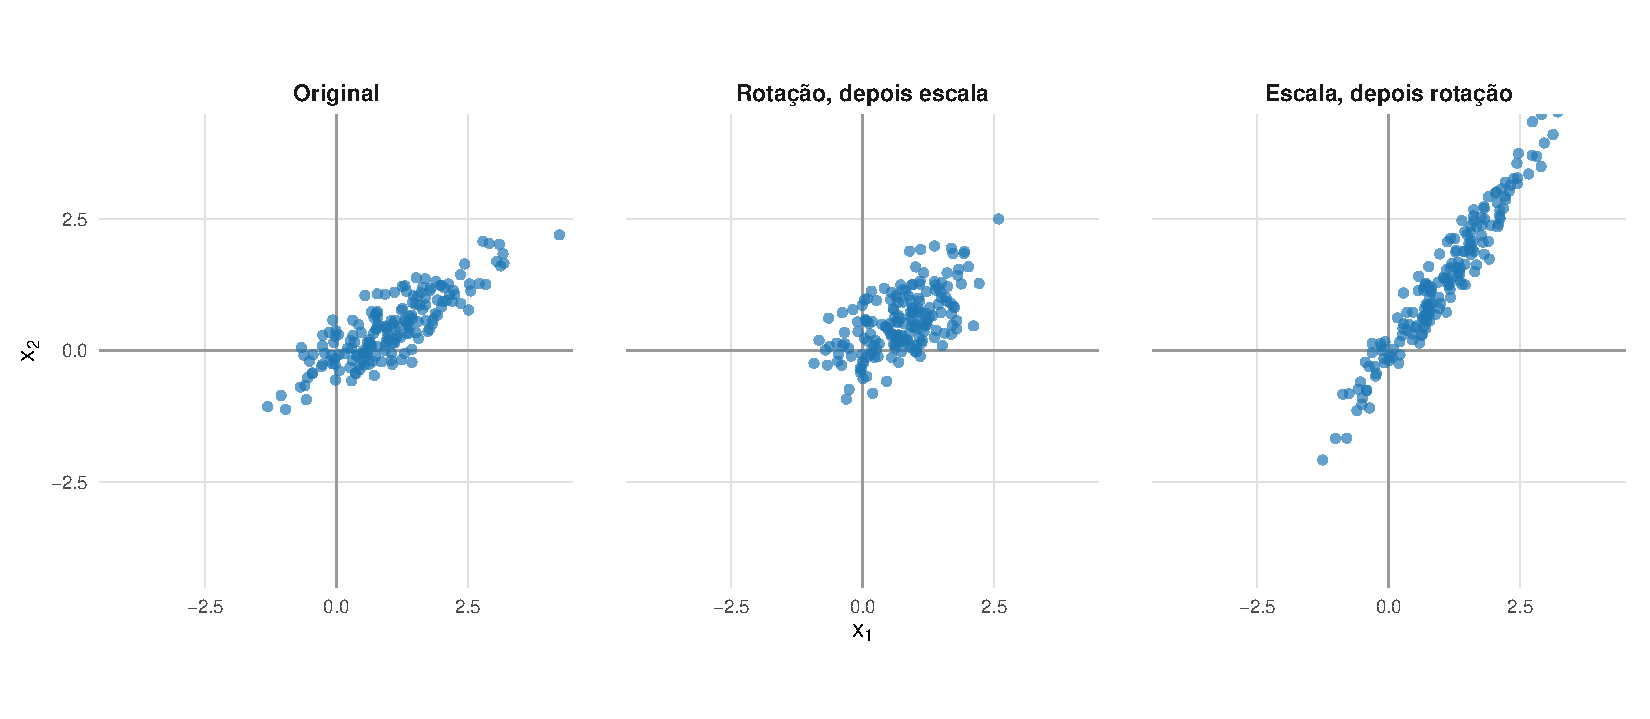
\includegraphics[keepaspectratio]{mod_1_transformacoes_files/figure-pdf/fig-composicao-transformacoes-1.pdf}}

}

\caption{\label{fig-composicao-transformacoes}Efeito da ordem na
composição de uma rotação e de um escalonamento não uniforme.}

\end{figure}%

As duas composições utilizam as mesmas transformações, mas produzem
configurações diferentes. Na primeira, a nuvem é rotacionada antes de
ser escalonada em relação aos eixos coordenados. Na segunda, o
escalonamento ocorre antes da mudança de orientação.

\subsection{Transformação inversa}\label{transformauxe7uxe3o-inversa}

Uma transformação linear invertível permite recuperar de maneira única o
vetor original a partir de sua imagem.

\begin{definition}[Transformação
inversa]\protect\hypertarget{def-transformacao-inversa}{}\label{def-transformacao-inversa}

Uma transformação linear

\[
T:
V
\longrightarrow
W
\]

é invertível quando existe uma transformação

\[
T^{-1}:
W
\longrightarrow
V
\]

tal que

\[
T^{-1}
\left(
T(\mathbf{x})
\right)
=
\mathbf{x}
\]

para todo \(\mathbf{x}\in V\) e

\[
T
\left(
T^{-1}(\mathbf{y})
\right)
=
\mathbf{y}
\]

para todo \(\mathbf{y}\in W\).

\end{definition}

Considere uma transformação

\[
T:
\mathbb{R}^p
\longrightarrow
\mathbb{R}^p
\]

representada por uma matriz quadrada e invertível

\[
\mathbf{A}
\in
\mathbb{R}^{p\times p}.
\]

Se

\[
\mathbf{y}
=
\mathbf{A}\mathbf{x},
\]

então

\[
\mathbf{x}
=
\mathbf{A}^{-1}\mathbf{y}.
\]

A transformação inversa é representada por \(\mathbf{A}^{-1}\).

\begin{proposition}[Inversa de uma
composição]\protect\hypertarget{prp-inversa-composicao}{}\label{prp-inversa-composicao}

Se \(\mathbf{A}\) e \(\mathbf{B}\) são matrizes quadradas e invertíveis
de dimensões compatíveis, então

\[
\left(
\mathbf{B}\mathbf{A}
\right)^{-1}
=
\mathbf{A}^{-1}
\mathbf{B}^{-1}.
\]

\end{proposition}

\begin{proof}
Tem-se

\[
\begin{aligned}
\left(
\mathbf{B}\mathbf{A}
\right)
\left(
\mathbf{A}^{-1}\mathbf{B}^{-1}
\right)
&=
\mathbf{B}
\left(
\mathbf{A}\mathbf{A}^{-1}
\right)
\mathbf{B}^{-1}\\
&=
\mathbf{B}\mathbf{B}^{-1}\\
&=
\mathbf{I}.
\end{aligned}
\]

De forma análoga,

\[
\begin{aligned}
\left(
\mathbf{A}^{-1}\mathbf{B}^{-1}
\right)
\left(
\mathbf{B}\mathbf{A}
\right)
&=
\mathbf{A}^{-1}
\left(
\mathbf{B}^{-1}\mathbf{B}
\right)
\mathbf{A}\\
&=
\mathbf{A}^{-1}\mathbf{A}\\
&=
\mathbf{I}.
\end{aligned}
\]

Logo,

\[
\left(
\mathbf{B}\mathbf{A}
\right)^{-1}
=
\mathbf{A}^{-1}
\mathbf{B}^{-1}.
\]
\end{proof}

A ordem é invertida porque a última transformação aplicada deve ser a
primeira a ser desfeita.

\subsection{Injetividade, sobrejetividade e
bijetividade}\label{injetividade-sobrejetividade-e-bijetividade}

As propriedades de injetividade e sobrejetividade descrevem,
respectivamente, a possibilidade de distinguir vetores do domínio por
suas imagens e a possibilidade de atingir todos os vetores do
contradomínio.

\begin{definition}[Injetividade, sobrejetividade e
bijetividade]\protect\hypertarget{def-injetividade-sobrejetividade}{}\label{def-injetividade-sobrejetividade}

Uma transformação

\[
T:
V
\longrightarrow
W
\]

é:

\begin{enumerate}
\def\labelenumi{\arabic{enumi}.}
\item
  \textbf{injetiva} quando

  \[
  T(\mathbf{x}_1)
  =
  T(\mathbf{x}_2)
  \quad\Longrightarrow\quad
  \mathbf{x}_1
  =
  \mathbf{x}_2;
  \]
\item
  \textbf{sobrejetiva} quando, para todo \(\mathbf{y}\in W\), existe
  pelo menos um \(\mathbf{x}\in V\) tal que

  \[
  T(\mathbf{x})
  =
  \mathbf{y};
  \]
\item
  \textbf{bijetiva} quando é simultaneamente injetiva e sobrejetiva.
\end{enumerate}

\end{definition}

Para uma transformação matricial

\[
T_{\mathbf{A}}:
\mathbb{R}^p
\longrightarrow
\mathbb{R}^q,
\qquad
T_{\mathbf{A}}(\mathbf{x})
=
\mathbf{A}\mathbf{x},
\]

essas propriedades podem ser caracterizadas pelo núcleo, pelo espaço
coluna e pelo posto.

\begin{proposition}[Caracterizações por núcleo, imagem e
posto]\protect\hypertarget{prp-caracterizacoes-transformacao-linear}{}\label{prp-caracterizacoes-transformacao-linear}

Seja

\[
T_{\mathbf{A}}:
\mathbb{R}^p
\longrightarrow
\mathbb{R}^q,
\qquad
T_{\mathbf{A}}(\mathbf{x})
=
\mathbf{A}\mathbf{x},
\]

com \(\mathbf{A}\in\mathbb{R}^{q\times p}\). Então:

\begin{enumerate}
\def\labelenumi{\arabic{enumi}.}
\item
  \(T_{\mathbf{A}}\) é injetiva se, e somente se,

  \[\ker(T_{\mathbf{A}})=\mathcal{N}(\mathbf{A})=\{\mathbf{0}\};\]
\item
  \(T_{\mathbf{A}}\) é injetiva se, e somente se,

  \[\operatorname{posto}(\mathbf{A})=p;\]
\item
  \(T_{\mathbf{A}}\) é sobrejetiva se, e somente se,

  \[\operatorname{Im}(T_{\mathbf{A}})=\mathcal{C}(\mathbf{A})=\mathbb{R}^q;\]
\item
  \(T_{\mathbf{A}}\) é sobrejetiva se, e somente se,

  \[\operatorname{posto}(\mathbf{A})=q.\]
\end{enumerate}

(Meyer, 2023)

\end{proposition}

\begin{proof}
Suponha inicialmente que \(T_{\mathbf{A}}\) seja injetiva. Se

\[\mathbf{x}\in\ker(T_{\mathbf{A}})=\mathcal{N}(\mathbf{A}),\]

então

\[\mathbf{A}\mathbf{x}=\mathbf{0}=\mathbf{A}\mathbf{0}.\]

Pela injetividade,

\[\mathbf{x}=\mathbf{0}.\]

Logo,

\[\ker(T_{\mathbf{A}})=\mathcal{N}(\mathbf{A})=\{\mathbf{0}\}.\]

Reciprocamente, suponha que

\[\ker(T_{\mathbf{A}})=\mathcal{N}(\mathbf{A})=\{\mathbf{0}\}\]

e que

\[\mathbf{A}\mathbf{x}_1=\mathbf{A}\mathbf{x}_2.\]

Então,

\[\mathbf{A}(\mathbf{x}_1-\mathbf{x}_2)=\mathbf{0}.\]

Portanto,

\[\mathbf{x}_1-\mathbf{x}_2\in\ker(T_{\mathbf{A}})=\mathcal{N}(\mathbf{A}),\]

o que implica

\[\mathbf{x}_1=\mathbf{x}_2.\]

Assim, \(T_{\mathbf{A}}\) é injetiva.

Pelo Teorema~\ref{thm-posto-nulidade},

\[\dim\mathcal{N}(\mathbf{A})+\operatorname{posto}(\mathbf{A})=p.\]

Como \(\mathcal{N}(\mathbf{A})=\ker(T_{\mathbf{A}})\), tem-se

\[\ker(T_{\mathbf{A}})=\{\mathbf{0}\}\]

se, e somente se,

\[\operatorname{posto}(\mathbf{A})=p.\]

Por outro lado, \(T_{\mathbf{A}}\) é sobrejetiva quando todo vetor de
\(\mathbb{R}^q\) pertence à sua imagem. Como

\[\operatorname{Im}(T_{\mathbf{A}})=\mathcal{C}(\mathbf{A}),\]

a sobrejetividade equivale a

\[\operatorname{Im}(T_{\mathbf{A}})=\mathcal{C}(\mathbf{A})=\mathbb{R}^q.\]

Essa igualdade ocorre se, e somente se,

\[\dim\mathcal{C}(\mathbf{A})=q,\]

isto é,

\[\operatorname{posto}(\mathbf{A})=q.\]
\end{proof}

Uma transformação de \(\mathbb{R}^p\) em \(\mathbb{R}^q\) pode ser
injetiva somente quando

\[
q
\geq
p.
\]

De forma análoga, pode ser sobrejetiva somente quando

\[
p
\geq
q.
\]

Se a transformação é bijetiva, então

\[
p=q
\]

e

\[
\operatorname{posto}(\mathbf{A})
=
p.
\]

Combinando o Proposição~\ref{prp-caracterizacoes-transformacao-linear}
com o Teorema~\ref{thm-equivalencias-invertibilidade}, obtém-se o
resultado seguinte.

\begin{proposition}[Equivalências para uma transformação linear
associada a uma matriz
quadrada]\protect\hypertarget{prp-equivalencias-transformacao-invertivel}{}\label{prp-equivalencias-transformacao-invertivel}

Considere

\[
\mathbf{A}
\in
\mathbb{R}^{p\times p}
\]

e a transformação linear

\[
T_{\mathbf{A}}:
\mathbb{R}^p
\longrightarrow
\mathbb{R}^p,
\qquad
T_{\mathbf{A}}(\mathbf{x})
=
\mathbf{A}\mathbf{x}.
\]

São equivalentes:

\begin{enumerate}
\def\labelenumi{\arabic{enumi}.}
\tightlist
\item
  \(T_{\mathbf{A}}\) é injetiva;
\item
  \(T_{\mathbf{A}}\) é sobrejetiva;
\item
  \(T_{\mathbf{A}}\) é bijetiva;
\item
  \(T_{\mathbf{A}}\) é invertível;
\item
  \(\mathcal{N}(\mathbf{A})=\{\mathbf{0}\}\);
\item
  \(\mathcal{C}(\mathbf{A})=\mathbb{R}^p\);
\item
  \(\operatorname{posto}(\mathbf{A})=p\);
\item
  \(\det(\mathbf{A})\neq0\);
\item
  \(\mathbf{A}^{-1}\) existe.
\end{enumerate}

(Meyer, 2023)

\end{proposition}

A Tabela~\ref{tbl-injetividade-sobrejetividade} resume as relações
principais.

\begin{longtable}[]{@{}
  >{\raggedright\arraybackslash}p{(\linewidth - 4\tabcolsep) * \real{0.3333}}
  >{\raggedright\arraybackslash}p{(\linewidth - 4\tabcolsep) * \real{0.3333}}
  >{\raggedright\arraybackslash}p{(\linewidth - 4\tabcolsep) * \real{0.3333}}@{}}
\caption{Relações entre injetividade, sobrejetividade, bijetividade e
posto.}\label{tbl-injetividade-sobrejetividade}\tabularnewline
\toprule\noalign{}
\begin{minipage}[b]{\linewidth}\raggedright
Propriedade
\end{minipage} & \begin{minipage}[b]{\linewidth}\raggedright
Condição geométrica
\end{minipage} & \begin{minipage}[b]{\linewidth}\raggedright
Condição matricial
\end{minipage} \\
\midrule\noalign{}
\endfirsthead
\toprule\noalign{}
\begin{minipage}[b]{\linewidth}\raggedright
Propriedade
\end{minipage} & \begin{minipage}[b]{\linewidth}\raggedright
Condição geométrica
\end{minipage} & \begin{minipage}[b]{\linewidth}\raggedright
Condição matricial
\end{minipage} \\
\midrule\noalign{}
\endhead
\bottomrule\noalign{}
\endlastfoot
Injetividade & Vetores distintos possuem imagens distintas &
\(\ker(T_{\mathbf{A}})=\mathcal{N}(\mathbf{A})=\{\mathbf{0}\}\) e
\(\operatorname{posto}(\mathbf{A})=p\) \\
Sobrejetividade & Todo vetor do contradomínio é atingido &
\(\operatorname{Im}(T_{\mathbf{A}})=\mathcal{C}(\mathbf{A})=\mathbb{R}^q\)
e \(\operatorname{posto}(\mathbf{A})=q\) \\
Bijetividade & Há correspondência única entre domínio e contradomínio &
\(p=q=\operatorname{posto}(\mathbf{A})\) \\
Invertibilidade & A transformação pode ser desfeita & \(\mathbf{A}\) é
quadrada e \(\det(\mathbf{A})\neq0\) \\
\end{longtable}

\subsection{Perda de informação}\label{perda-de-informauxe7uxe3o}

Quando a transformação não é injetiva, existem vetores distintos com a
mesma imagem.

Se

\[\mathbf{v}\in\ker(T_{\mathbf{A}})=\mathcal{N}(\mathbf{A}),\]

então, para qualquer \(\mathbf{x}\in\mathbb{R}^p\),

\[
\begin{aligned}
\mathbf{A}
\left(
\mathbf{x}+\mathbf{v}
\right)
&=
\mathbf{A}\mathbf{x}
+
\mathbf{A}\mathbf{v}\\
&=
\mathbf{A}\mathbf{x}.
\end{aligned}
\]

Portanto, todos os vetores do conjunto

\[
\mathbf{x}
+
\ker(T_{\mathbf{A}})
=
\left\{
\mathbf{x}+\mathbf{v}:
\mathbf{v}\in\ker(T_{\mathbf{A}})
\right\}
\]

produzem a mesma imagem.

Reciprocamente, se

\[
\mathbf{A}\mathbf{x}_1
=
\mathbf{A}\mathbf{x}_2,
\]

então

\[
\mathbf{x}_1-\mathbf{x}_2
\in
\mathcal{N}(\mathbf{A}).
\]

A ambiguidade na recuperação do vetor original é, assim, determinada
pelo núcleo da transformação, que coincide com o espaço nulo da matriz
associada.

Se

\[
\operatorname{posto}(\mathbf{A})
=
r,
\]

o Teorema Posto--Nulidade fornece

\[
\dim
\left(
\mathcal{N}(\mathbf{A})
\right)
=
p-r.
\]

O espaço nulo possui dimensão \(p-r\). Portanto, existem \(p-r\)
direções linearmente independentes no domínio que são anuladas pela
transformação, enquanto a imagem possui dimensão \(r\).

\subsection{Redução de
dimensionalidade}\label{reduuxe7uxe3o-de-dimensionalidade}

Considere

\[
\mathbf{A}
\in
\mathbb{R}^{q\times p}
\]

com

\[
q<p.
\]

Mesmo que

\[
\operatorname{posto}(\mathbf{A})
=
q,
\]

tem-se

\[
\dim
\left(
\mathcal{N}(\mathbf{A})
\right)
=
p-q
>
0.
\]

A perda de informação é inevitável quando a transformação é considerada
sobre todo o espaço \(\mathbb{R}^p\). Entretanto, sua restrição a um
conjunto particular ou a um subespaço de dimensão menor ou igual a \(q\)
pode ser injetiva. Assim, reduzir o número de coordenadas não implica
necessariamente identificar observações distintas no conjunto de dados
efetivamente analisado.

A redução pode ser útil quando a matriz é escolhida para preservar
determinadas direções e eliminar outras. O critério utilizado para
selecionar essas direções será desenvolvido posteriormente, no contexto
das técnicas multivariadas.

\subsection{Transformações
singulares}\label{transformauxe7uxf5es-singulares}

Uma matriz quadrada é singular quando

\[
\det(\mathbf{A})
=
0.
\]

Nesse caso,

\[
\operatorname{posto}(\mathbf{A})
<
p,
\]

e a transformação leva \(\mathbb{R}^p\) a um subespaço de menor
dimensão.

Por exemplo,

\[
\mathbf{A}
=
\begin{bmatrix}
1&0\\
0&0
\end{bmatrix}
\]

transforma

\[
\begin{bmatrix}
x_1\\
x_2
\end{bmatrix}
\]

em

\[
\begin{bmatrix}
x_1\\
0
\end{bmatrix}.
\]

Todos os pontos com a mesma primeira coordenada produzem a mesma imagem.

A Figura~\ref{fig-inversibilidade} compara uma transformação invertível,
a recuperação pela inversa e uma transformação singular.

\begin{figure}

\centering{

\pandocbounded{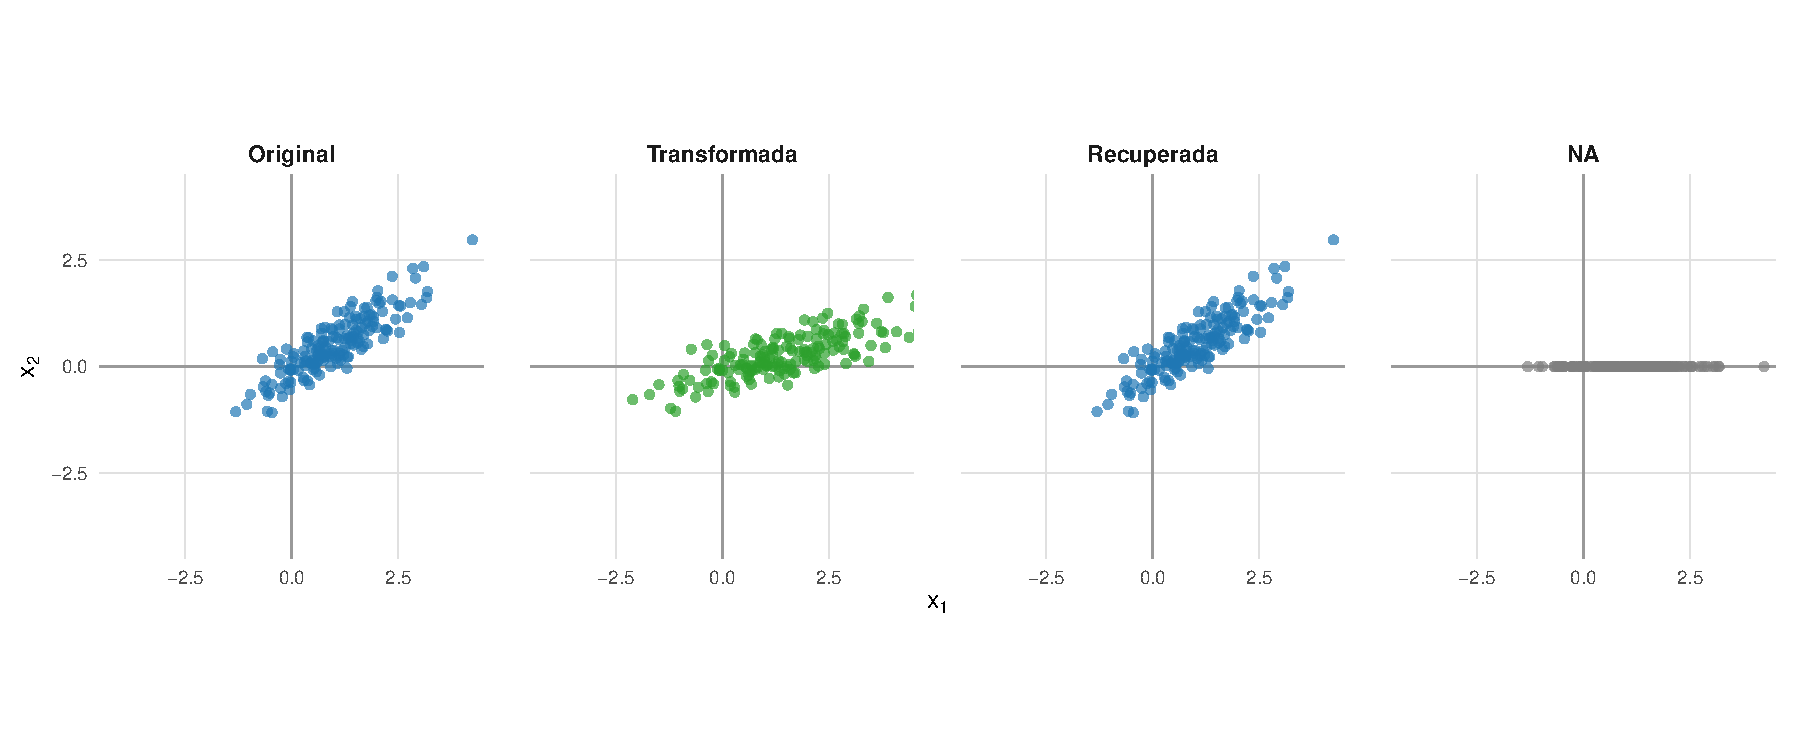
\includegraphics[keepaspectratio]{mod_1_transformacoes_files/figure-pdf/fig-inversibilidade-1.pdf}}

}

\caption{\label{fig-inversibilidade}Transformação invertível,
recuperação pela inversa e colapso provocado por uma transformação
singular.}

\end{figure}%

A transformação representada por \(\mathbf{A}\) modifica a configuração,
mas mantém uma correspondência única entre os pontos originais e
transformados. A aplicação de \(\mathbf{A}^{-1}\) recupera a
configuração inicial. A transformação singular elimina a segunda
coordenada e reduz toda a nuvem a uma reta.

Para

\[
T_{\mathbf{A}}:
\mathbb{R}^p
\longrightarrow
\mathbb{R}^q,
\]

as possibilidades podem ser resumidas da seguinte forma:

\begin{itemize}
\tightlist
\item
  se \(q<p\), a transformação não pode ser injetiva;
\item
  se \(q>p\), a transformação não pode ser sobrejetiva;
\item
  se \(q=p\), ela é bijetiva quando
  \(\operatorname{posto}(\mathbf{A})=p\);
\item
  se \(\operatorname{posto}(\mathbf{A})<\min(p,q)\), ela não é injetiva
  nem sobrejetiva.
\end{itemize}

Essas relações permitem interpretar

\[
\operatorname{posto}(\mathbf{A})
\]

como a dimensão da imagem da transformação, isto é, como o número máximo
de direções linearmente independentes que podem compor o espaço
transformado. A seção seguinte examina os efeitos geométricos produzidos
por classes particulares de matrizes.

\section{Transformações
geométricas}\label{transformauxe7uxf5es-geomuxe9tricas}

Matrizes distintas produzem efeitos geométricos diferentes sobre vetores
e conjuntos de pontos. Algumas modificam a posição da configuração em
relação aos eixos coordenados sem deformar sua geometria, enquanto
outras alteram comprimentos, ângulos, áreas ou dimensão.

Nesta seção, são examinadas cinco transformações no plano:

\begin{itemize}
\tightlist
\item
  rotação;
\item
  reflexão;
\item
  escalonamento;
\item
  cisalhamento;
\item
  projeção.
\end{itemize}

Todas preservam combinações lineares e, portanto, são transformações
lineares. As propriedades geométricas preservadas dependem da matriz
utilizada.

\subsection{Rotação}\label{rotauxe7uxe3o}

Uma rotação de ângulo \(\theta\) em torno da origem é representada por

\[
\mathbf{Q}_\theta
=
\begin{bmatrix}
\cos\theta&-\sin\theta\\
\sin\theta&\cos\theta
\end{bmatrix}.
\]

Para

\[
\mathbf{x}
=
\begin{bmatrix}
x_1\\
x_2
\end{bmatrix},
\]

a imagem é

\[
\mathbf{y}
=
\mathbf{Q}_\theta\mathbf{x},
\]

isto é,

\[
\begin{aligned}
y_1
&=
x_1\cos\theta
-
x_2\sin\theta,\\
y_2
&=
x_1\sin\theta
+
x_2\cos\theta.
\end{aligned}
\]

A matriz de rotação satisfaz

\[
\mathbf{Q}_\theta^{\top}
\mathbf{Q}_\theta
=
\mathbf{I}_2.
\]

Consequentemente,

\[
\mathbf{Q}_\theta^{-1}
=
\mathbf{Q}_\theta^{\top}
=
\mathbf{Q}_{-\theta}.
\]

A transformação inversa corresponde a uma rotação pelo mesmo ângulo no
sentido oposto.

Além disso,

\[
\det
\left(
\mathbf{Q}_\theta
\right)
=
1.
\]

A rotação preserva comprimentos, distâncias, ângulos, áreas e
orientação.

\subsection{Reflexão}\label{reflexuxe3o}

Uma reflexão no plano produz a imagem especular dos vetores em relação a
uma reta que passa pela origem.

A reflexão em relação ao eixo horizontal é representada por

\[
\mathbf{F}_1
=
\begin{bmatrix}
1&0\\
0&-1
\end{bmatrix},
\]

de modo que

\[
\begin{bmatrix}
x_1\\
x_2
\end{bmatrix}
\longmapsto
\begin{bmatrix}
x_1\\
-x_2
\end{bmatrix}.
\]

A reflexão em relação ao eixo vertical é representada por

\[
\mathbf{F}_2
=
\begin{bmatrix}
-1&0\\
0&1
\end{bmatrix},
\]

e produz

\[
\begin{bmatrix}
x_1\\
x_2
\end{bmatrix}
\longmapsto
\begin{bmatrix}
-x_1\\
x_2
\end{bmatrix}.
\]

As duas matrizes satisfazem

\[
\mathbf{F}^{\top}\mathbf{F}
=
\mathbf{I}_2
\]

e

\[
\mathbf{F}^{-1}
=
\mathbf{F}.
\]

Assim,

\[
\mathbf{F}^2
=
\mathbf{I}_2.
\]

Aplicar duas vezes a mesma reflexão recupera o vetor original.

Considere agora uma reta gerada por um vetor unitário

\[
\mathbf{u}
\in
\mathbb{R}^2,
\qquad
\|\mathbf{u}\|
=
1.
\]

A projeção de \(\mathbf{x}\) sobre essa reta é

\[
\mathbf{u}\mathbf{u}^{\top}\mathbf{x},
\]

enquanto sua componente ortogonal é

\[
\left(
\mathbf{I}_2
-
\mathbf{u}\mathbf{u}^{\top}
\right)
\mathbf{x}.
\]

Na reflexão, a componente paralela é preservada e a componente ortogonal
tem seu sinal invertido:

\[
\begin{aligned}
\mathbf{x}_{\mathrm{ref}}
&=
\mathbf{u}\mathbf{u}^{\top}\mathbf{x}
-
\left(
\mathbf{I}_2
-
\mathbf{u}\mathbf{u}^{\top}
\right)
\mathbf{x}\\
&=
\left(
2\mathbf{u}\mathbf{u}^{\top}
-
\mathbf{I}_2
\right)
\mathbf{x}.
\end{aligned}
\]

Portanto, a reflexão em relação à reta gerada por \(\mathbf{u}\) é
representada por

\[
\mathbf{F}_{\mathbf{u}}
=
2\mathbf{u}\mathbf{u}^{\top}
-
\mathbf{I}_2.
\]

Essa matriz satisfaz

\[
\mathbf{F}_{\mathbf{u}}^{\top}
\mathbf{F}_{\mathbf{u}}
=
\mathbf{I}_2
\]

e

\[
\det
\left(
\mathbf{F}_{\mathbf{u}}
\right)
=
-1.
\]

A reflexão preserva comprimentos, distâncias, ângulos e áreas, mas
inverte a orientação.

Em dimensão \(p\), a matriz

\[
\mathbf{H}_{\mathbf{u}}
=
\mathbf{I}_p
-
2\mathbf{u}\mathbf{u}^{\top},
\qquad
\|\mathbf{u}\|=1,
\]

representa a reflexão em relação ao hiperplano ortogonal a
\(\mathbf{u}\). Essa transformação é denominada \textbf{reflexão de
Householder}.

Observe que as duas construções preservam componentes diferentes. A
matriz \(2\mathbf{u}\mathbf{u}^{\top}-\mathbf{I}\) preserva a componente
na direção de \(\mathbf{u}\) e inverte as componentes ortogonais a ela,
enquanto \(\mathbf{I}-2\mathbf{u}\mathbf{u}^{\top}\) preserva as
componentes ortogonais a \(\mathbf{u}\) e inverte a componente na
direção de \(\mathbf{u}\).

\subsection{Escalonamento}\label{escalonamento}

Um escalonamento modifica o comprimento dos vetores ao longo de direções
determinadas.

No plano, o escalonamento em relação aos eixos coordenados é
representado por

\[
\mathbf{L}
=
\begin{bmatrix}
s_1&0\\
0&s_2
\end{bmatrix}.
\]

A transformação correspondente é

\[
\begin{bmatrix}
x_1\\
x_2
\end{bmatrix}
\longmapsto
\begin{bmatrix}
s_1x_1\\
s_2x_2
\end{bmatrix}.
\]

Quando

\[
s_1
=
s_2
=
s,
\]

o escalonamento é uniforme:

\[
\mathbf{L}
=
s\mathbf{I}_2.
\]

Nesse caso, todos os comprimentos e todas as distâncias são
multiplicados por \(|s|\). Para \(s\neq0\), os ângulos são preservados.

Quando

\[s_1\neq s_2,\]

o escalonamento é não uniforme. Cada direção coordenada é reescalada por
um fator próprio, de modo que comprimentos, ângulos e proporções podem
ser alterados. Se algum fator \(s_j\) for negativo, além da alteração de
escala ocorre a inversão do sentido da coordenada correspondente.

O determinante da matriz é

\[
\det(\mathbf{L})
=
s_1s_2.
\]

A área de uma figura é, portanto, multiplicada por

\[
|s_1s_2|.
\]

A transformação é invertível quando

\[
s_1\neq0
\qquad
\text{e}
\qquad
s_2\neq0.
\]

Nesse caso,

\[
\mathbf{L}^{-1}
=
\begin{bmatrix}
1/s_1&0\\
0&1/s_2
\end{bmatrix}.
\]

Se algum fator de escala for igual a zero, uma direção é eliminada. Por
exemplo,

\[
\mathbf{L}
=
\begin{bmatrix}
1&0\\
0&0
\end{bmatrix}
\]

leva todo o plano ao eixo horizontal.

O escalonamento das variáveis será retomado na seção sobre
pré-processamento.

\subsection{Cisalhamento}\label{cisalhamento}

Um cisalhamento modifica uma coordenada adicionando a ela uma parcela
proporcional a outra coordenada.

O cisalhamento horizontal é representado por

\[
\mathbf{C}_{12}(k)
=
\begin{bmatrix}
1&k\\
0&1
\end{bmatrix}.
\]

Nesse caso,

\[
\begin{aligned}
y_1
&=
x_1+kx_2,\\
y_2
&=
x_2.
\end{aligned}
\]

A segunda coordenada permanece inalterada, enquanto a primeira é
modificada de acordo com o valor de \(x_2\).

O cisalhamento vertical é representado por

\[
\mathbf{C}_{21}(k)
=
\begin{bmatrix}
1&0\\
k&1
\end{bmatrix},
\]

e produz

\[
\begin{aligned}
y_1
&=
x_1,\\
y_2
&=
kx_1+x_2.
\end{aligned}
\]

Em dimensão \(p\), um cisalhamento elementar pode ser escrito como

\[
\mathbf{C}_{ij}(k)
=
\mathbf{I}_p
+
k\mathbf{e}_i\mathbf{e}_j^{\top},
\qquad
i\neq j.
\]

Essa transformação adiciona à coordenada \(i\) uma parcela proporcional
à coordenada \(j\).

Como

\[
\left(
\mathbf{e}_i\mathbf{e}_j^{\top}
\right)^2
=
\mathbf{0}
\]

para \(i\neq j\), tem-se

\[
\begin{aligned}
\mathbf{C}_{ij}(k)
\mathbf{C}_{ij}(-k)
&=
\left(
\mathbf{I}_p
+
k\mathbf{e}_i\mathbf{e}_j^{\top}
\right)
\left(
\mathbf{I}_p
-
k\mathbf{e}_i\mathbf{e}_j^{\top}
\right)\\
&=
\mathbf{I}_p.
\end{aligned}
\]

Portanto,

\[
\mathbf{C}_{ij}(k)^{-1}
=
\mathbf{C}_{ij}(-k).
\]

O determinante de um cisalhamento elementar é

\[
\det
\left(
\mathbf{C}_{ij}(k)
\right)
=
1.
\]

Assim, o cisalhamento preserva áreas e volumes, mas altera comprimentos
e ângulos. Retas e paralelismo são preservados.

\subsection{Projeção}\label{projeuxe7uxe3o}

As projeções ortogonais foram desenvolvidas no capítulo anterior a
partir da decomposição de um vetor em componentes pertencentes a
subespaços ortogonais. Aqui, interessa interpretá-las como
transformações lineares.

Considere uma direção unitária

\[\mathbf{u}\in\mathbb{R}^p,\qquad \|\mathbf{u}\|=1,\]

e o subespaço

\[S=\operatorname{span}\{\mathbf{u}\}.\]

A matriz da projeção ortogonal sobre \(S\) é

\[\mathbf{P}_{S}=\mathbf{u}\mathbf{u}^{\top},\]

de modo que

\[T_{\mathbf{P}_{S}}(\mathbf{x})=\mathbf{P}_{S}\mathbf{x}.\]

Como estudado no capítulo anterior,

\[\mathbf{P}_{S}^2=\mathbf{P}_{S}\]

e

\[\mathbf{P}_{S}^{\top}=\mathbf{P}_{S}.\]

Do ponto de vista das transformações lineares,

\[\operatorname{Im}(T_{\mathbf{P}_{S}})=S\]

e

\[\ker(T_{\mathbf{P}_{S}})=S^{\perp}.\]

Assim, a projeção preserva a componente pertencente a \(S\) e elimina
toda a componente pertencente a \(S^{\perp}\).

Para uma projeção sobre uma única direção,

\[\operatorname{posto}(\mathbf{P}_{S})=1.\]

Consequentemente, quando \(p>1\),

\[\det(\mathbf{P}_{S})=0,\]

e a transformação não é invertível. Vetores que diferem apenas por uma
componente pertencente a \(S^{\perp}\) possuem a mesma imagem.

\subsection{Comparação geométrica}\label{comparauxe7uxe3o-geomuxe9trica}

A Figura~\ref{fig-transformacoes-quadrado} mostra o efeito das
transformações anteriores sobre o quadrado unitário. Como todos os
painéis utilizam a mesma escala, alterações de forma, área e dimensão
podem ser comparadas diretamente.

\begin{figure}

\centering{

\pandocbounded{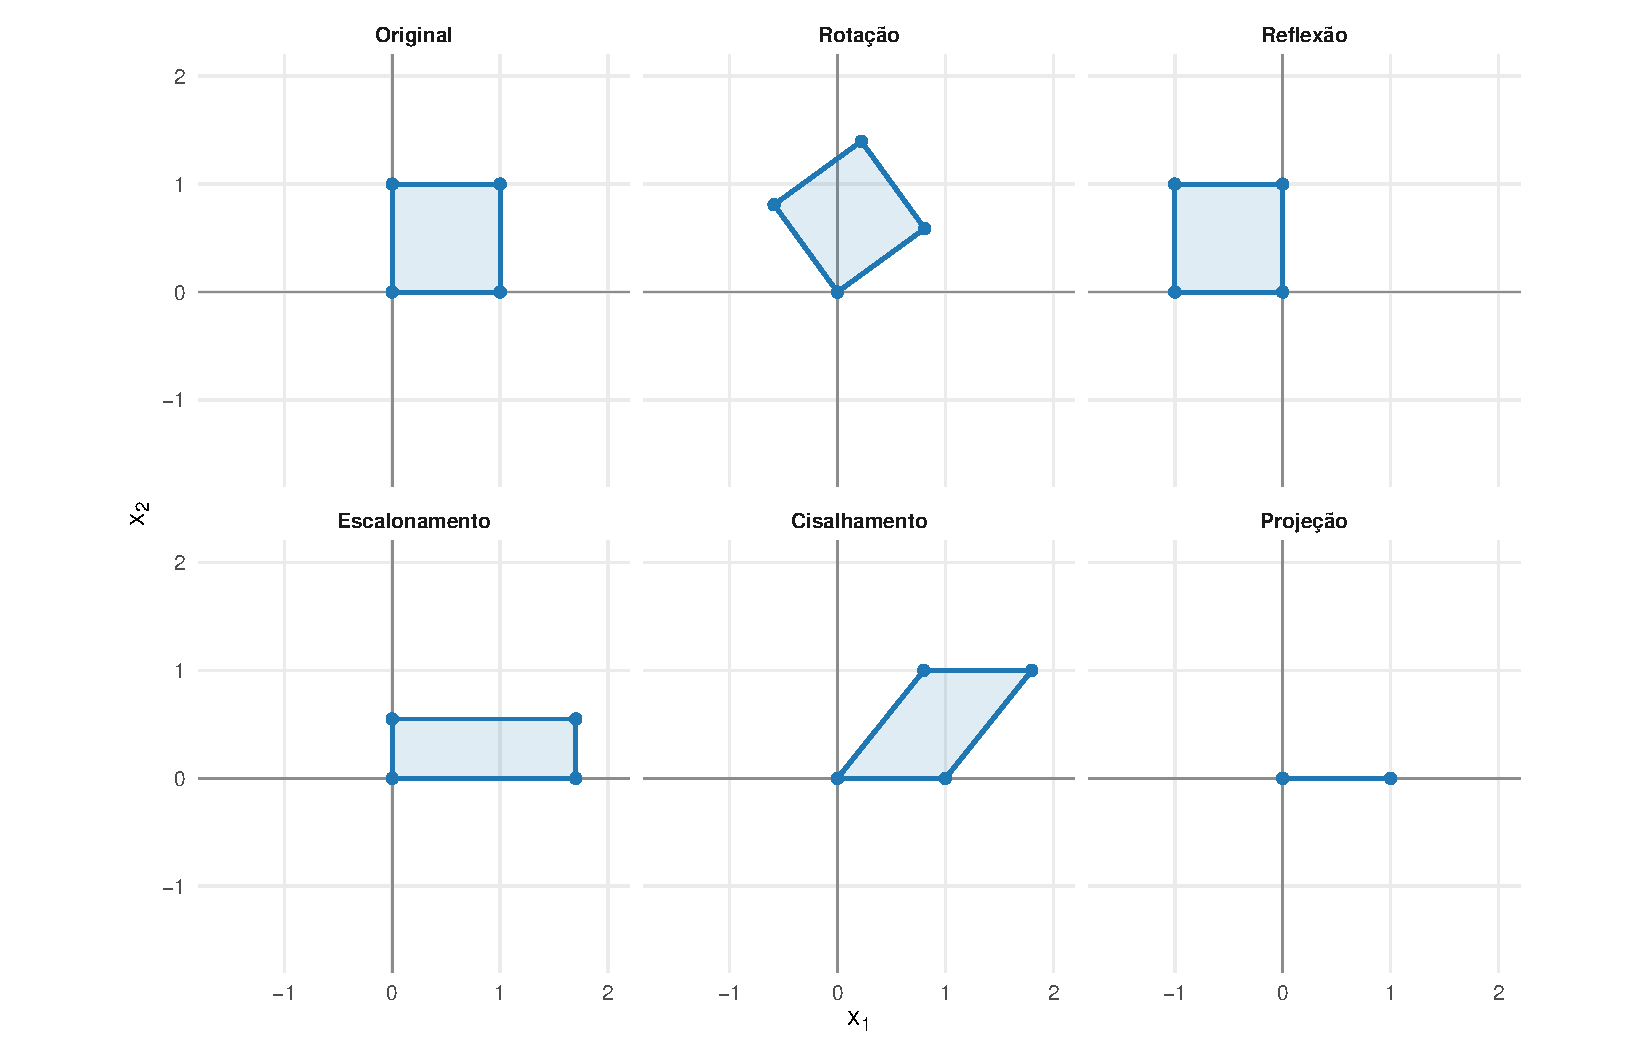
\includegraphics[keepaspectratio]{mod_1_transformacoes_files/figure-pdf/fig-transformacoes-quadrado-1.pdf}}

}

\caption{\label{fig-transformacoes-quadrado}Efeito de diferentes
transformações lineares sobre o quadrado unitário.}

\end{figure}%

A rotação altera a posição do quadrado em relação aos eixos coordenados
sem modificar sua forma, sua área ou sua orientação. A reflexão preserva
a forma e a área, mas inverte a orientação. O escalonamento não uniforme
modifica os comprimentos nas direções coordenadas e transforma o
quadrado em um retângulo. O cisalhamento transforma o quadrado em um
paralelogramo com a mesma área, mostrando que preservar área não implica
preservar ângulos ou comprimentos. A projeção elimina uma direção e
reduz a figura a um segmento de reta.

\subsection{Determinante, volume e
orientação}\label{determinante-volume-e-orientauxe7uxe3o}

Para uma matriz quadrada

\[
\mathbf{A}
\in
\mathbb{R}^{p\times p},
\]

o valor absoluto do determinante representa o fator pelo qual volumes
são multiplicados.

\begin{proposition}[Alteração de volume por uma transformação
linear]\protect\hypertarget{prp-determinante-volume-transformacao}{}\label{prp-determinante-volume-transformacao}

Seja

\[
\mathbf{A}
\in
\mathbb{R}^{p\times p}
\]

e seja

\[
E
\subseteq
\mathbb{R}^p
\]

um conjunto mensurável com volume \(p\)-dimensional finito. Denote por

\[
\mathbf{A}E
=
\left\{
\mathbf{A}\mathbf{x}:
\mathbf{x}\in E
\right\}
\]

sua imagem pela transformação linear representada por \(\mathbf{A}\).

Então,

\[
\operatorname{Vol}_p
\left(
\mathbf{A}E
\right)
=
|\det(\mathbf{A})|
\operatorname{Vol}_p(E),
\]

em que \(\operatorname{Vol}_p\) representa o volume \(p\)-dimensional.

Se

\[
\det(\mathbf{A})
=
0,
\]

então

\[
\operatorname{posto}(\mathbf{A})
<
p,
\]

de modo que a imagem \(\mathbf{A}E\) está contida em um subespaço
próprio de \(\mathbb{R}^p\). Consequentemente,

\[
\operatorname{Vol}_p
\left(
\mathbf{A}E
\right)
=
0.
\]

\end{proposition}

A demonstração formal desse resultado, baseada no Jacobiano de uma
transformação linear, será apresentada no capítulo dedicado ao cálculo
multivariado.

No plano, o resultado descreve a alteração de área. Em \(\mathbb{R}^3\),
descreve a alteração de volume. Em dimensão geral, descreve a alteração
do hipervolume.

Quando a transformação é invertível, o sinal do determinante descreve o
efeito sobre a orientação:

\begin{itemize}
\tightlist
\item
  se \(\det(\mathbf{A})>0\), a orientação é preservada;
\item
  se \(\det(\mathbf{A})<0\), a orientação é invertida.
\end{itemize}

Se \(\det(\mathbf{A})=0\), a transformação não é invertível, sua imagem
possui dimensão inferior a \(p\) e o volume \(p\)-dimensional é reduzido
a zero.

A Tabela~\ref{tbl-transformacoes-geometricas} resume as propriedades das
transformações estudadas.

\begin{longtable}[]{@{}
  >{\raggedright\arraybackslash}p{(\linewidth - 6\tabcolsep) * \real{0.2394}}
  >{\raggedright\arraybackslash}p{(\linewidth - 6\tabcolsep) * \real{0.2394}}
  >{\centering\arraybackslash}p{(\linewidth - 6\tabcolsep) * \real{0.2817}}
  >{\raggedright\arraybackslash}p{(\linewidth - 6\tabcolsep) * \real{0.2394}}@{}}
\caption{Propriedades das principais transformações geométricas no
plano.}\label{tbl-transformacoes-geometricas}\tabularnewline
\toprule\noalign{}
\begin{minipage}[b]{\linewidth}\raggedright
Transformação
\end{minipage} & \begin{minipage}[b]{\linewidth}\raggedright
Matriz no plano
\end{minipage} & \begin{minipage}[b]{\linewidth}\centering
Determinante
\end{minipage} & \begin{minipage}[b]{\linewidth}\raggedright
Efeito geométrico
\end{minipage} \\
\midrule\noalign{}
\endfirsthead
\toprule\noalign{}
\begin{minipage}[b]{\linewidth}\raggedright
Transformação
\end{minipage} & \begin{minipage}[b]{\linewidth}\raggedright
Matriz no plano
\end{minipage} & \begin{minipage}[b]{\linewidth}\centering
Determinante
\end{minipage} & \begin{minipage}[b]{\linewidth}\raggedright
Efeito geométrico
\end{minipage} \\
\midrule\noalign{}
\endhead
\bottomrule\noalign{}
\endlastfoot
Rotação & \(\mathbf{Q}_\theta\) & \(1\) & Gira a configuração \\
Reflexão & \(\mathbf{F}\) & \(-1\) & Produz uma imagem especular \\
Escalonamento & \(\operatorname{diag}(s_1,s_2)\) & \(s_1s_2\) & Reescala
direções coordenadas \\
Cisalhamento & \(\begin{bmatrix}1&k\\0&1\end{bmatrix}\) & \(1\) &
Inclina a configuração \\
Projeção sobre uma reta & \(\mathbf{u}\mathbf{u}^{\top}\) & \(0\) &
Elimina uma direção \\
\end{longtable}

A preservação de área ou volume não implica preservação de distâncias e
ângulos. O cisalhamento possui determinante igual a 1, mas deforma a
configuração. A preservação integral da geometria euclidiana será
estudada na seção seguinte.

\section{Transformações
ortogonais}\label{transformauxe7uxf5es-ortogonais}

A linearidade não garante a preservação de comprimentos, distâncias ou
ângulos. Essas propriedades são preservadas pelas transformações
representadas por matrizes ortogonais.

Retomando a Definição~\ref{def-matriz-ortogonal}, uma matriz

\[
\mathbf{Q}
\in
\mathbb{R}^{p\times p}
\]

é ortogonal quando

\[
\mathbf{Q}^{\top}\mathbf{Q}
=
\mathbf{I}_p.
\]

Essa condição implica

\[
\mathbf{Q}^{-1}
=
\mathbf{Q}^{\top}
\]

e

\[
\mathbf{Q}\mathbf{Q}^{\top}
=
\mathbf{I}_p.
\]

A transformação

\[
T_{\mathbf{Q}}:
\mathbb{R}^p
\longrightarrow
\mathbb{R}^p,
\qquad
T_{\mathbf{Q}}(\mathbf{x})
=
\mathbf{Q}\mathbf{x},
\]

é denominada \textbf{transformação ortogonal}.

\begin{proposition}[Preservação da geometria
euclidiana]\protect\hypertarget{prp-preservacao-geometria-transformacao-ortogonal}{}\label{prp-preservacao-geometria-transformacao-ortogonal}

Se \(\mathbf{Q}\in\mathbb{R}^{p\times p}\) é ortogonal, então, para
quaisquer \(\mathbf{x},\mathbf{y}\in\mathbb{R}^p\), a transformação

\[T_{\mathbf{Q}}(\mathbf{x})=\mathbf{Q}\mathbf{x}\]

preserva:

\begin{enumerate}
\def\labelenumi{\arabic{enumi}.}
\tightlist
\item
  o produto interno;
\item
  as normas;
\item
  as distâncias euclidianas;
\item
  os ângulos entre vetores não nulos;
\item
  a ortogonalidade.
\end{enumerate}

\end{proposition}

\begin{proof}
Pelo Teorema~\ref{thm-preservacao-produto-interno},

\[
\left(
\mathbf{Q}\mathbf{x}
\right)^{\top}
\left(
\mathbf{Q}\mathbf{y}
\right)
=
\mathbf{x}^{\top}\mathbf{y}.
\]

Portanto, o produto interno entre quaisquer dois vetores é preservado.

Tomando \(\mathbf{y}=\mathbf{x}\),

\[
\begin{aligned}
\|\mathbf{Q}\mathbf{x}\|^2
&=
\left(
\mathbf{Q}\mathbf{x}
\right)^{\top}
\left(
\mathbf{Q}\mathbf{x}
\right)\\
&=
\mathbf{x}^{\top}\mathbf{x}\\
&=
\|\mathbf{x}\|^2.
\end{aligned}
\]

Como as normas são não negativas,

\[\|\mathbf{Q}\mathbf{x}\|=\|\mathbf{x}\|.\]

Para dois vetores \(\mathbf{x}\) e \(\mathbf{y}\),

\[
\begin{aligned}
\|
\mathbf{Q}\mathbf{x}
-
\mathbf{Q}\mathbf{y}
\|
&=
\|
\mathbf{Q}
(\mathbf{x}-\mathbf{y})
\|\\
&=
\|
\mathbf{x}-\mathbf{y}
\|.
\end{aligned}
\]

Logo, todas as distâncias euclidianas entre pares de vetores são
preservadas.

Para vetores não nulos, o ângulo \(\theta\) entre \(\mathbf{x}\) e
\(\mathbf{y}\) é determinado por

\[
\cos(\theta)
=
\frac{
\mathbf{x}^{\top}\mathbf{y}
}{
\|\mathbf{x}\|
\,
\|\mathbf{y}\|
}.
\]

Como o produto interno e as normas são preservados,

\[
\frac{
\left(
\mathbf{Q}\mathbf{x}
\right)^{\top}
\left(
\mathbf{Q}\mathbf{y}
\right)
}{
\|\mathbf{Q}\mathbf{x}\|
\,
\|\mathbf{Q}\mathbf{y}\|
}
=
\frac{
\mathbf{x}^{\top}\mathbf{y}
}{
\|\mathbf{x}\|
\,
\|\mathbf{y}\|
}.
\]

Portanto, os ângulos também são preservados.

Em particular, se

\[\mathbf{x}^{\top}\mathbf{y}=0,\]

então

\[
\left(
\mathbf{Q}\mathbf{x}
\right)^{\top}
\left(
\mathbf{Q}\mathbf{y}
\right)
=
0,
\]

e a ortogonalidade é preservada.
\end{proof}

Assim, transformações ortogonais preservam integralmente as relações
métricas determinadas pelo produto interno euclidiano. Elas podem
alterar a orientação da configuração, mas não deformam sua geometria
interna.

\subsection{Transformação de uma matriz de
dados}\label{transformauxe7uxe3o-de-uma-matriz-de-dados-1}

Considere uma matriz de dados

\[
\mathbf{X}
\in
\mathbb{R}^{n\times p}
\]

e uma transformação ortogonal representada por

\[
\mathbf{Q}
\in
\mathbb{R}^{p\times p}.
\]

Como as observações estão organizadas nas linhas, a matriz transformada
é

\[
\mathbf{Y}
=
\mathbf{X}\mathbf{Q}^{\top}.
\]

\begin{proposition}[Preservação da matriz de
Gram]\protect\hypertarget{prp-gram-transformacao-ortogonal}{}\label{prp-gram-transformacao-ortogonal}

Se

\[
\mathbf{Y}
=
\mathbf{X}\mathbf{Q}^{\top}
\]

e \(\mathbf{Q}\) é ortogonal, então

\[
\mathbf{Y}\mathbf{Y}^{\top}
=
\mathbf{X}\mathbf{X}^{\top}.
\]

\end{proposition}

\begin{proof}
Tem-se

\[
\begin{aligned}
\mathbf{Y}\mathbf{Y}^{\top}
&=
\left(
\mathbf{X}\mathbf{Q}^{\top}
\right)
\left(
\mathbf{X}\mathbf{Q}^{\top}
\right)^{\top}\\
&=
\mathbf{X}
\mathbf{Q}^{\top}
\mathbf{Q}
\mathbf{X}^{\top}\\
&=
\mathbf{X}
\mathbf{I}_p
\mathbf{X}^{\top}\\
&=
\mathbf{X}\mathbf{X}^{\top}.
\end{aligned}
\]
\end{proof}

A matriz de Gram reúne os produtos internos entre as observações. Sua
preservação implica que permanecem inalterados:

\begin{itemize}
\tightlist
\item
  os quadrados das normas das observações;
\item
  os produtos internos entre pares de observações;
\item
  as distâncias entre as observações;
\item
  os ângulos entre os vetores observados não nulos.
\end{itemize}

A nuvem de pontos pode ser rotacionada ou refletida, mas sua forma e
suas relações internas permanecem as mesmas.

\subsection{Determinante e
orientação}\label{determinante-e-orientauxe7uxe3o}

\begin{proposition}[Determinante de uma matriz
ortogonal]\protect\hypertarget{prp-determinante-matriz-ortogonal}{}\label{prp-determinante-matriz-ortogonal}

Se \(\mathbf{Q}\in\mathbb{R}^{p\times p}\) é ortogonal, então

\[\det(\mathbf{Q})\in\{-1,1\}.\]

Consequentemente,

\[|\det(\mathbf{Q})|=1,\]

e a transformação preserva volumes \(p\)-dimensionais.

\end{proposition}

\begin{proof}
Como

\[\mathbf{Q}^{\top}\mathbf{Q}=\mathbf{I}_p,\]

tem-se

\[
\begin{aligned}
1
&=
\det
\left(
\mathbf{Q}^{\top}\mathbf{Q}
\right)\\
&=
\det
\left(
\mathbf{Q}^{\top}
\right)
\det(\mathbf{Q})\\
&=
\det(\mathbf{Q})^2.
\end{aligned}
\]

Portanto,

\[\det(\mathbf{Q})=1\qquad\text{ou}\qquad\det(\mathbf{Q})=-1.\]

Logo,

\[|\det(\mathbf{Q})|=1.\]
\end{proof}

No plano, a preservação do volume \(p\)-dimensional corresponde à
preservação de áreas; em \(\mathbb{R}^3\), corresponde à preservação de
volumes.

Quando

\[
\det(\mathbf{Q})
=
1,
\]

a transformação é denominada \textbf{ortogonal própria}. Ela preserva a
orientação.

No plano, toda transformação ortogonal própria é uma rotação e pode ser
representada por

\[
\mathbf{Q}
=
\begin{bmatrix}
\cos\theta&-\sin\theta\\
\sin\theta&\cos\theta
\end{bmatrix}.
\]

Quando

\[
\det(\mathbf{Q})
=
-1,
\]

a transformação é denominada \textbf{ortogonal imprópria}. Ela inverte a
orientação.

No plano, toda transformação ortogonal imprópria corresponde a uma
reflexão em relação a uma reta que passa pela origem. Em dimensões
superiores, pode combinar uma reflexão com rotações em subespaços
ortogonais.

\subsection{Matrizes ortogonais e bases
ortonormais}\label{matrizes-ortogonais-e-bases-ortonormais}

As colunas de uma matriz ortogonal formam uma base ortonormal de
\(\mathbb{R}^p\).

Se

\[
\mathbf{Q}
=
\begin{bmatrix}
\mathbf{q}_1&
\mathbf{q}_2&
\cdots&
\mathbf{q}_p
\end{bmatrix},
\]

então suas colunas satisfazem

\[\mathbf{q}_i^{\top}\mathbf{q}_j=\delta_{ij},\]

em que \(\delta_{ij}\) é o delta de Kronecker definido no Capítulo 2.
Portanto, as colunas de \(\mathbf{Q}\) possuem norma unitária e são
ortogonais duas a duas.

Como

\[\mathbf{Q}\mathbf{Q}^{\top}=\mathbf{I}_p,\]

as linhas de \(\mathbf{Q}\) também formam um conjunto ortonormal.

Uma matriz ortogonal admite, portanto, duas interpretações que devem ser
distinguidas:

\begin{itemize}
\tightlist
\item
  como matriz de uma transformação linear que preserva a geometria
  euclidiana;
\item
  como matriz cujas colunas constituem uma base ortonormal de
  \(\mathbb{R}^p\).
\end{itemize}

Na primeira interpretação, a matriz atua sobre o vetor e modifica sua
posição no espaço. Na segunda, seus vetores-coluna definem um sistema de
coordenadas. A relação entre essas duas interpretações será desenvolvida
na seção seguinte.

\subsection{Comparação com transformações não
ortogonais}\label{comparauxe7uxe3o-com-transformauxe7uxf5es-nuxe3o-ortogonais}

A Figura~\ref{fig-transformacoes-ortogonais} compara o efeito de
diferentes matrizes sobre a circunferência unitária e sobre duas
direções inicialmente ortogonais. O marcador de ângulo reto identifica
os casos em que a ortogonalidade é preservada.

\begin{figure}

\centering{

\pandocbounded{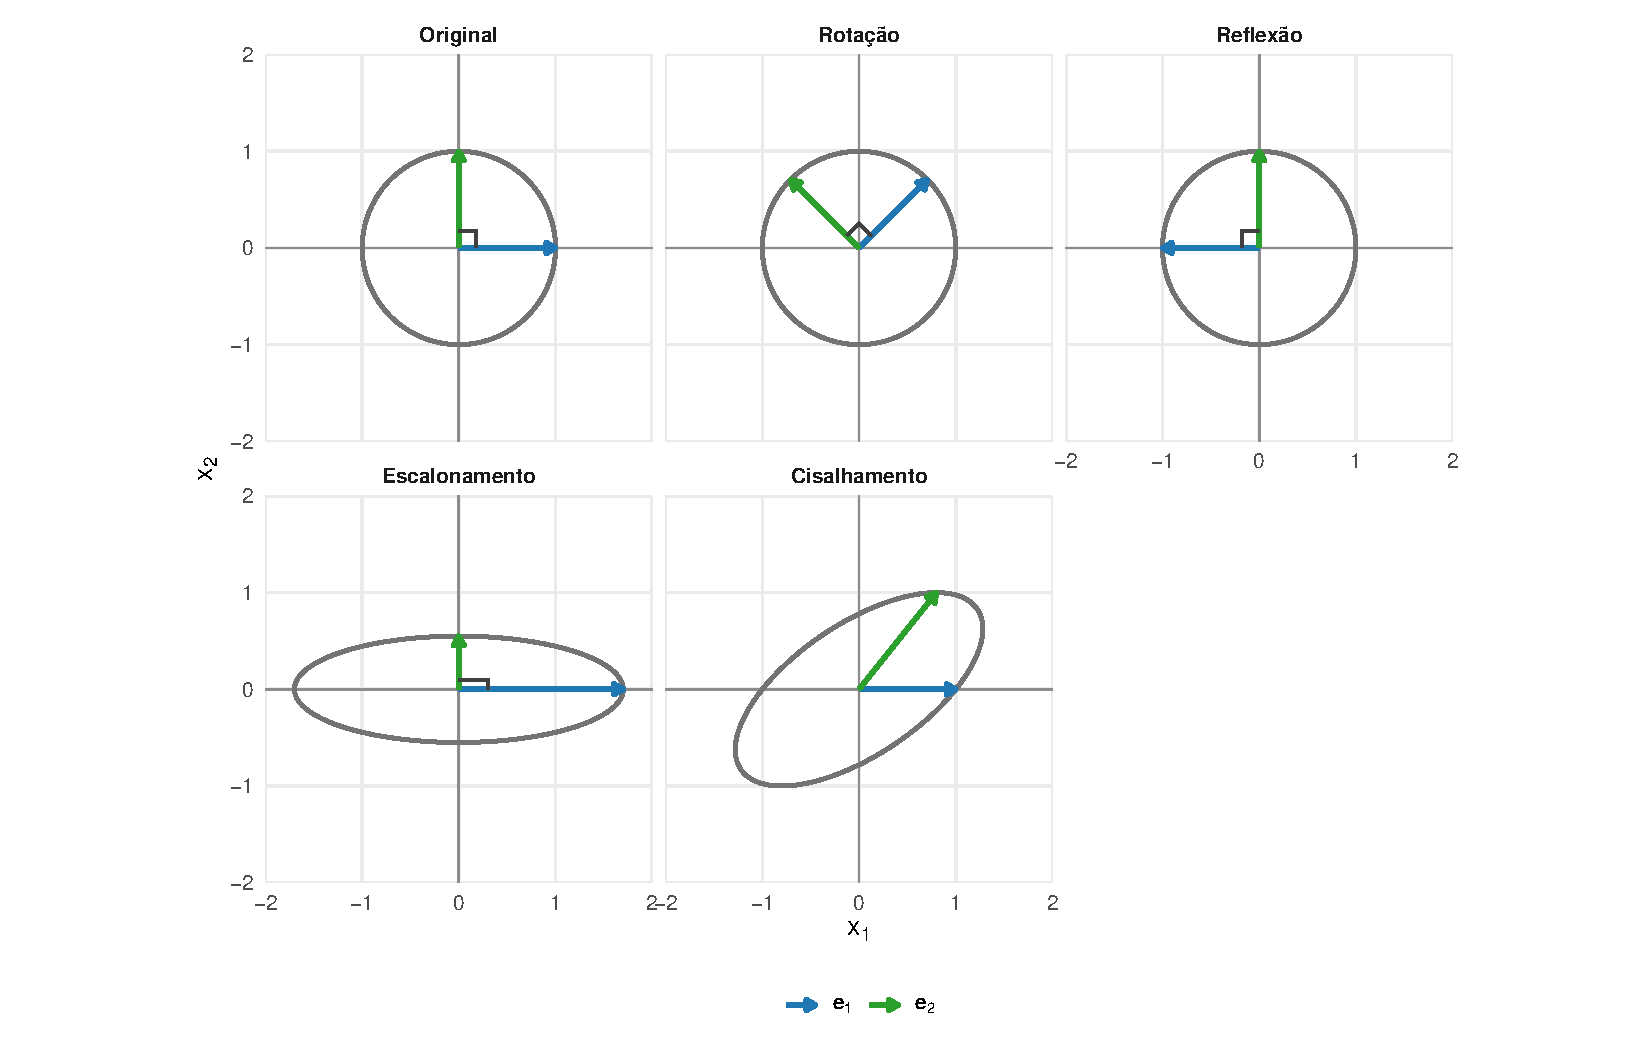
\includegraphics[keepaspectratio]{mod_1_transformacoes_files/figure-pdf/fig-transformacoes-ortogonais-1.pdf}}

}

\caption{\label{fig-transformacoes-ortogonais}Efeito de transformações
ortogonais e não ortogonais sobre a circunferência unitária e duas
direções inicialmente ortogonais.}

\end{figure}%

A rotação e a reflexão mantêm a circunferência unitária e preservam o
ângulo reto entre as duas direções. O escalonamento não uniforme
transforma a circunferência em uma elipse; embora as duas direções
coordenadas permaneçam ortogonais neste exemplo particular, seus
comprimentos são alterados e a transformação não é ortogonal. O
cisalhamento deforma a circunferência e também altera o ângulo entre as
direções.

A Tabela~\ref{tbl-transformacoes-ortogonais} compara as propriedades
dessas transformações.

\begin{longtable}[]{@{}
  >{\raggedright\arraybackslash}p{(\linewidth - 10\tabcolsep) * \real{0.1667}}
  >{\centering\arraybackslash}p{(\linewidth - 10\tabcolsep) * \real{0.1667}}
  >{\centering\arraybackslash}p{(\linewidth - 10\tabcolsep) * \real{0.1667}}
  >{\centering\arraybackslash}p{(\linewidth - 10\tabcolsep) * \real{0.1667}}
  >{\centering\arraybackslash}p{(\linewidth - 10\tabcolsep) * \real{0.1667}}
  >{\centering\arraybackslash}p{(\linewidth - 10\tabcolsep) * \real{0.1667}}@{}}
\caption{Comparação entre transformações ortogonais e não
ortogonais.}\label{tbl-transformacoes-ortogonais}\tabularnewline
\toprule\noalign{}
\begin{minipage}[b]{\linewidth}\raggedright
Transformação
\end{minipage} & \begin{minipage}[b]{\linewidth}\centering
Ortogonal
\end{minipage} & \begin{minipage}[b]{\linewidth}\centering
Preserva normas
\end{minipage} & \begin{minipage}[b]{\linewidth}\centering
Preserva distâncias
\end{minipage} & \begin{minipage}[b]{\linewidth}\centering
Preserva ângulos
\end{minipage} & \begin{minipage}[b]{\linewidth}\centering
\(|\det(\mathbf{A})|\)
\end{minipage} \\
\midrule\noalign{}
\endfirsthead
\toprule\noalign{}
\begin{minipage}[b]{\linewidth}\raggedright
Transformação
\end{minipage} & \begin{minipage}[b]{\linewidth}\centering
Ortogonal
\end{minipage} & \begin{minipage}[b]{\linewidth}\centering
Preserva normas
\end{minipage} & \begin{minipage}[b]{\linewidth}\centering
Preserva distâncias
\end{minipage} & \begin{minipage}[b]{\linewidth}\centering
Preserva ângulos
\end{minipage} & \begin{minipage}[b]{\linewidth}\centering
\(|\det(\mathbf{A})|\)
\end{minipage} \\
\midrule\noalign{}
\endhead
\bottomrule\noalign{}
\endlastfoot
Rotação & Sim & Sim & Sim & Sim & \(1\) \\
Reflexão & Sim & Sim & Sim & Sim & \(1\) \\
Escalonamento uniforme & Somente se \(|s|=1\) & Somente se \(|s|=1\) &
Somente se \(|s|=1\) & Sim, se \(s\neq0\) & \(|s|^p\) \\
Escalonamento não uniforme & Não & Não & Não & Não, em geral &
\(\prod_j|s_j|\) \\
Cisalhamento & Não & Não & Não & Não, em geral & \(1\) \\
Projeção própria & Não & Não & Não & Não, em geral & \(0\) \\
\end{longtable}

A condição

\[
|\det(\mathbf{A})|
=
1
\]

não é suficiente para que uma matriz seja ortogonal. O cisalhamento
possui determinante igual a 1 e preserva áreas, mas não preserva normas
nem ângulos.

A condição que caracteriza a preservação da geometria euclidiana é

\[
\mathbf{A}^{\top}\mathbf{A}
=
\mathbf{I}_p.
\]

\section{Mudanças de coordenadas e representação em
bases}\label{mudanuxe7as-de-coordenadas-e-representauxe7uxe3o-em-bases}

O Capítulo 3 mostrou que um vetor possui coordenadas diferentes quando é
representado em bases distintas. O vetor geométrico permanece o mesmo; o
que muda é o conjunto de coeficientes utilizado para descrevê-lo.

Retomando a Definição~\ref{def-coordenadas-base}, seja

\[
\mathcal{B}
=
\{
\mathbf{b}_1,\ldots,\mathbf{b}_p
\}
\]

uma base de \(\mathbb{R}^p\), com a ordem dos vetores fixada. Como
definido no capítulo anterior, a matriz formada pelos vetores da base é

\[
\mathbf{B}
=
\begin{bmatrix}
\mathbf{b}_1&
\cdots&
\mathbf{b}_p
\end{bmatrix}.
\]

Como os vetores de \(\mathcal{B}\) são linearmente independentes,
\(\mathbf{B}\) é invertível.

Se

\[
[\mathbf{x}]_{\mathcal{B}}
=
\begin{bmatrix}
c_1\\
\vdots\\
c_p
\end{bmatrix}
\]

é o vetor de coordenadas de \(\mathbf{x}\) na base \(\mathcal{B}\),
então

\[\mathbf{x}=c_1\mathbf{b}_1+\cdots+c_p\mathbf{b}_p.\]

Em forma matricial,

\[\mathbf{x}=\mathbf{B}[\mathbf{x}]_{\mathcal{B}}.\]

Consequentemente,

\[[\mathbf{x}]_{\mathcal{B}}=\mathbf{B}^{-1}\mathbf{x}.\]

Assim, \(\mathbf{B}\) converte as coordenadas de \(\mathbf{x}\) na base
\(\mathcal{B}\) em suas coordenadas na base canônica, enquanto
\(\mathbf{B}^{-1}\) realiza a conversão no sentido contrário.

Quando \(\mathcal{B}\) é uma base ortonormal, pela
Definição~\ref{def-base-ortonormal},

\[\mathbf{B}^{\top}\mathbf{B}=\mathbf{I}_p.\]

Logo,

\[\mathbf{B}^{-1}=\mathbf{B}^{\top}\]

e

\[[\mathbf{x}]_{\mathcal{B}}=\mathbf{B}^{\top}\mathbf{x}.\]

Nesse caso,

\[
[\mathbf{x}]_{\mathcal{B}}
=
\begin{bmatrix}
\mathbf{b}_1^{\top}\mathbf{x}\\
\vdots\\
\mathbf{b}_p^{\top}\mathbf{x}
\end{bmatrix},
\]

de modo que cada coordenada é obtida pelo produto interno entre
\(\mathbf{x}\) e o vetor correspondente da base.

\subsection{Conversão entre duas
bases}\label{conversuxe3o-entre-duas-bases}

Considere duas bases de \(\mathbb{R}^p\),

\[
\mathcal{B}
=
\{
\mathbf{b}_1,\ldots,\mathbf{b}_p
\}
\]

e

\[
\mathcal{C}
=
\{
\mathbf{c}_1,\ldots,\mathbf{c}_p
\},
\]

e as respectivas matrizes

\[
\mathbf{B}
=
\begin{bmatrix}
\mathbf{b}_1&
\cdots&
\mathbf{b}_p
\end{bmatrix}
\]

e

\[
\mathbf{C}
=
\begin{bmatrix}
\mathbf{c}_1&
\cdots&
\mathbf{c}_p
\end{bmatrix}.
\]

O mesmo vetor pode ser representado por

\[\mathbf{x}=\mathbf{B}[\mathbf{x}]_{\mathcal{B}}\]

e por

\[\mathbf{x}=\mathbf{C}[\mathbf{x}]_{\mathcal{C}}.\]

Igualando as duas expressões,

\[
\mathbf{C}
[\mathbf{x}]_{\mathcal{C}}
=
\mathbf{B}
[\mathbf{x}]_{\mathcal{B}}.
\]

Multiplicando à esquerda por \(\mathbf{C}^{-1}\),

\[
[\mathbf{x}]_{\mathcal{C}}
=
\mathbf{C}^{-1}
\mathbf{B}
[\mathbf{x}]_{\mathcal{B}}.
\]

\begin{definition}[Matriz de mudança de
base]\protect\hypertarget{def-matriz-mudanca-base}{}\label{def-matriz-mudanca-base}

A \textbf{matriz de mudança de base de \(\mathcal{B}\) para
\(\mathcal{C}\)} é

\[\mathbf{C}^{-1}\mathbf{B}.\]

Ela transforma as coordenadas de um vetor na base \(\mathcal{B}\) em
suas coordenadas na base \(\mathcal{C}\):

\[
[\mathbf{x}]_{\mathcal{C}}
=
\left(
\mathbf{C}^{-1}\mathbf{B}
\right)
[\mathbf{x}]_{\mathcal{B}}.
\]

\end{definition}

O sentido da conversão deve ser observado na ordem das matrizes:

\[
\mathcal{B}
\longrightarrow
\mathcal{C}
\qquad\Longleftrightarrow\qquad
\mathbf{C}^{-1}\mathbf{B}.
\]

No sentido contrário, a matriz de mudança de base é

\[\mathbf{B}^{-1}\mathbf{C}.\]

As duas matrizes são inversas entre si:

\[
\mathbf{B}^{-1}\mathbf{C}
=
\left(
\mathbf{C}^{-1}\mathbf{B}
\right)^{-1}.
\]

\subsection{Representação de uma transformação em bases
gerais}\label{representauxe7uxe3o-de-uma-transformauxe7uxe3o-em-bases-gerais}

Considere uma transformação linear

\[
T:
\mathbb{R}^p
\longrightarrow
\mathbb{R}^q
\]

representada nas bases canônicas por

\[\mathbf{y}=\mathbf{A}\mathbf{x},\]

com

\[\mathbf{A}\in\mathbb{R}^{q\times p}.\]

Seja \(\mathcal{B}\) uma base do domínio, com matriz

\[
\mathbf{B}
=
\begin{bmatrix}
\mathbf{b}_1&
\cdots&
\mathbf{b}_p
\end{bmatrix},
\]

e seja \(\mathcal{C}\) uma base do contradomínio, com matriz

\[
\mathbf{C}
=
\begin{bmatrix}
\mathbf{c}_1&
\cdots&
\mathbf{c}_q
\end{bmatrix}.
\]

Como

\[\mathbf{x}=\mathbf{B}[\mathbf{x}]_{\mathcal{B}},\]

tem-se

\[
\begin{aligned}
[T(\mathbf{x})]_{\mathcal{C}}
&=
\mathbf{C}^{-1}
T(\mathbf{x})\\
&=
\mathbf{C}^{-1}
\mathbf{A}\mathbf{x}\\
&=
\mathbf{C}^{-1}
\mathbf{A}
\mathbf{B}
[\mathbf{x}]_{\mathcal{B}}.
\end{aligned}
\]

\begin{proposition}[Matriz de uma transformação em bases
gerais]\protect\hypertarget{prp-transformacao-bases-gerais}{}\label{prp-transformacao-bases-gerais}

Se uma transformação linear

\[
T:
\mathbb{R}^p
\longrightarrow
\mathbb{R}^q
\]

é representada nas bases canônicas por \(\mathbf{A}\), sua matriz em
relação à base \(\mathcal{B}\) do domínio e à base \(\mathcal{C}\) do
contradomínio é

\[
[T]_{\mathcal{C}\leftarrow\mathcal{B}}
=
\mathbf{C}^{-1}
\mathbf{A}
\mathbf{B}.
\]

Para todo \(\mathbf{x}\in\mathbb{R}^p\),

\[
[T(\mathbf{x})]_{\mathcal{C}}
=
[T]_{\mathcal{C}\leftarrow\mathcal{B}}
[\mathbf{x}]_{\mathcal{B}}.
\]

(Meyer, 2023)

\end{proposition}

A fórmula pode ser interpretada pela sequência das operações, da direita
para a esquerda:

\[
[\mathbf{x}]_{\mathcal{B}}
\xrightarrow{\ \mathbf{B}\ }
\mathbf{x}
\xrightarrow{\ \mathbf{A}\ }
T(\mathbf{x})
\xrightarrow{\ \mathbf{C}^{-1}\ }
[T(\mathbf{x})]_{\mathcal{C}}.
\]

As colunas de

\[[T]_{\mathcal{C}\leftarrow\mathcal{B}}\]

são as coordenadas, na base \(\mathcal{C}\), das imagens dos vetores da
base \(\mathcal{B}\):

\[
[T]_{\mathcal{C}\leftarrow\mathcal{B}}
=
\begin{bmatrix}
[T(\mathbf{b}_1)]_{\mathcal{C}}&
\cdots&
[T(\mathbf{b}_p)]_{\mathcal{C}}
\end{bmatrix}.
\]

Essa construção generaliza a representação matricial nas bases
canônicas.

\begin{example}[Representação de uma transformação em bases
distintas]\protect\hypertarget{exm-transformacao-bases-distintas}{}\label{exm-transformacao-bases-distintas}

Considere

\[
T:
\mathbb{R}^2
\longrightarrow
\mathbb{R}^2
\]

representada na base canônica por

\[
\mathbf{A}
=
\begin{bmatrix}
2&0\\
1&1
\end{bmatrix}.
\]

Considere a base do domínio

\[
\mathcal{B}
=
\left\{
\begin{bmatrix}
1\\
1
\end{bmatrix},
\begin{bmatrix}
1\\
0
\end{bmatrix}
\right\}
\]

e a base do contradomínio

\[
\mathcal{C}
=
\left\{
\begin{bmatrix}
1\\
0
\end{bmatrix},
\begin{bmatrix}
1\\
1
\end{bmatrix}
\right\}.
\]

As matrizes das bases são

\[
\mathbf{B}
=
\begin{bmatrix}
1&1\\
1&0
\end{bmatrix}
\]

e

\[
\mathbf{C}
=
\begin{bmatrix}
1&1\\
0&1
\end{bmatrix}.
\]

Como

\[
\mathbf{C}^{-1}
=
\begin{bmatrix}
1&-1\\
0&1
\end{bmatrix},
\]

tem-se

\[
\begin{aligned}
[T]_{\mathcal{C}\leftarrow\mathcal{B}}
&=
\mathbf{C}^{-1}
\mathbf{A}
\mathbf{B}\\
&=
\begin{bmatrix}
1&-1\\
0&1
\end{bmatrix}
\begin{bmatrix}
2&0\\
1&1
\end{bmatrix}
\begin{bmatrix}
1&1\\
1&0
\end{bmatrix}\\
&=
\begin{bmatrix}
0&1\\
2&1
\end{bmatrix}.
\end{aligned}
\]

A primeira coluna é

\[
[T(\mathbf{b}_1)]_{\mathcal{C}}
=
\begin{bmatrix}
0\\
2
\end{bmatrix},
\]

e a segunda é

\[
[T(\mathbf{b}_2)]_{\mathcal{C}}
=
\begin{bmatrix}
1\\
1
\end{bmatrix}.
\]

\end{example}

\subsection{Representação de um operador em uma nova
base}\label{representauxe7uxe3o-de-um-operador-em-uma-nova-base}

Considere um operador linear

\[
T:
\mathbb{R}^p
\longrightarrow
\mathbb{R}^p
\]

representado na base canônica por \(\mathbf{A}\).

Quando a mesma base \(\mathcal{B}\) é utilizada no domínio e no
contradomínio,

\[
[T]_{\mathcal{B}\leftarrow\mathcal{B}}
=
\mathbf{B}^{-1}
\mathbf{A}
\mathbf{B}.
\]

Quando conveniente, essa matriz será denotada abreviadamente por

\[
\mathbf{A}_{\mathcal{B}}
=
\mathbf{B}^{-1}
\mathbf{A}
\mathbf{B}.
\]

\begin{definition}[Matrizes
semelhantes]\protect\hypertarget{def-matrizes-semelhantes}{}\label{def-matrizes-semelhantes}

Duas matrizes quadradas \(\mathbf{A}\) e \(\mathbf{D}\) são
\textbf{semelhantes} quando existe uma matriz invertível \(\mathbf{P}\)
tal que

\[\mathbf{D}=\mathbf{P}^{-1}\mathbf{A}\mathbf{P}.\]

\end{definition}

Matrizes semelhantes representam o mesmo operador linear em bases
diferentes. Por essa razão, preservam propriedades que não dependem do
sistema de coordenadas.

\begin{proposition}[Invariantes por
semelhança]\protect\hypertarget{prp-invariantes-semelhanca}{}\label{prp-invariantes-semelhanca}

Sejam

\[
\mathbf{A},
\mathbf{D},
\mathbf{P}
\in
\mathbb{R}^{p\times p},
\]

com \(\mathbf{P}\) invertível. Se

\[\mathbf{D}=\mathbf{P}^{-1}\mathbf{A}\mathbf{P},\]

então

\[
\det(\mathbf{D})
=
\det(\mathbf{A}),
\]

\[
\operatorname{tr}(\mathbf{D})
=
\operatorname{tr}(\mathbf{A})
\]

e

\[
\operatorname{posto}(\mathbf{D})
=
\operatorname{posto}(\mathbf{A}).
\] (Horn; Johnson, 2013)

\end{proposition}

\begin{proof}
Para o determinante,

\[
\begin{aligned}
\det(\mathbf{D})
&=
\det
\left(
\mathbf{P}^{-1}
\mathbf{A}
\mathbf{P}
\right)\\
&=
\det
\left(
\mathbf{P}^{-1}
\right)
\det(\mathbf{A})
\det(\mathbf{P})\\
&=
\det(\mathbf{A}).
\end{aligned}
\]

Para o traço, pela propriedade cíclica,

\[
\begin{aligned}
\operatorname{tr}(\mathbf{D})
&=
\operatorname{tr}
\left(
\mathbf{P}^{-1}
\mathbf{A}
\mathbf{P}
\right)\\
&=
\operatorname{tr}
\left(
\mathbf{A}
\mathbf{P}
\mathbf{P}^{-1}
\right)\\
&=
\operatorname{tr}(\mathbf{A}).
\end{aligned}
\]

Como a multiplicação à esquerda ou à direita por uma matriz invertível
não altera o posto,

\[
\operatorname{posto}
\left(
\mathbf{P}^{-1}
\mathbf{A}
\mathbf{P}
\right)
=
\operatorname{posto}(\mathbf{A}).
\]
\end{proof}

A relação entre matrizes semelhantes, autovalores e a representação das
direções invariantes em bases diferentes será desenvolvida no capítulo
seguinte.

\subsection{Transformação ativa e mudança
passiva}\label{transformauxe7uxe3o-ativa-e-mudanuxe7a-passiva}

Uma matriz pode representar a transformação de um vetor ou a alteração
do sistema de coordenadas utilizado para descrevê-lo. Essas operações
são relacionadas, mas não são idênticas.

Em uma \textbf{transformação ativa}, os eixos coordenados permanecem
fixos e o vetor é modificado:

\[
\mathbf{y}
=
\mathbf{Q}\mathbf{x}.
\]

No caso de uma rotação, o vetor muda de posição em relação aos mesmos
eixos.

Em uma \textbf{mudança passiva de coordenadas}, o vetor geométrico
permanece fixo e a base é alterada.

Se as colunas de uma matriz ortogonal \(\mathbf{Q}\) formam a nova base

\[
\mathcal{B}
=
\{
\mathbf{q}_1,\ldots,\mathbf{q}_p
\},
\]

então

\[
[\mathbf{x}]_{\mathcal{B}}
=
\mathbf{Q}^{\top}\mathbf{x}
=
\mathbf{Q}^{-1}\mathbf{x}.
\]

O vetor não se move. Apenas sua representação numérica é modificada.

Para a matriz de rotação \(\mathbf{Q}_\theta\),

\[
\mathbf{Q}_\theta^{-1}
=
\mathbf{Q}_\theta^{\top}
=
\mathbf{Q}(-\theta).
\]

Girar os eixos pelo ângulo \(\theta\) transforma as coordenadas do vetor
por uma rotação de ângulo \(-\theta\).

A transformação ativa e a mudança passiva utilizam matrizes inversas:

\[
\text{transformação ativa:}
\qquad
\mathbf{y}
=
\mathbf{Q}\mathbf{x},
\]

\[
\text{mudança passiva:}
\qquad
[\mathbf{x}]_{\mathcal{B}}
=
\mathbf{Q}^{-1}\mathbf{x}.
\]

Quando \(\mathbf{Q}\) é ortogonal,

\[\mathbf{Q}^{-1}=\mathbf{Q}^{\top}.\]

Portanto, embora uma mesma matriz ortogonal possa aparecer nas duas
interpretações, o sentido da operação é distinto: na transformação
ativa, \(\mathbf{Q}\) atua sobre o vetor; na mudança passiva para a base
formada pelas colunas de \(\mathbf{Q}\), a conversão das coordenadas é
realizada por \(\mathbf{Q}^{-1}=\mathbf{Q}^{\top}\).

A Figura~\ref{fig-ativa-passiva} compara as duas interpretações.

\begin{figure}

\centering{

\pandocbounded{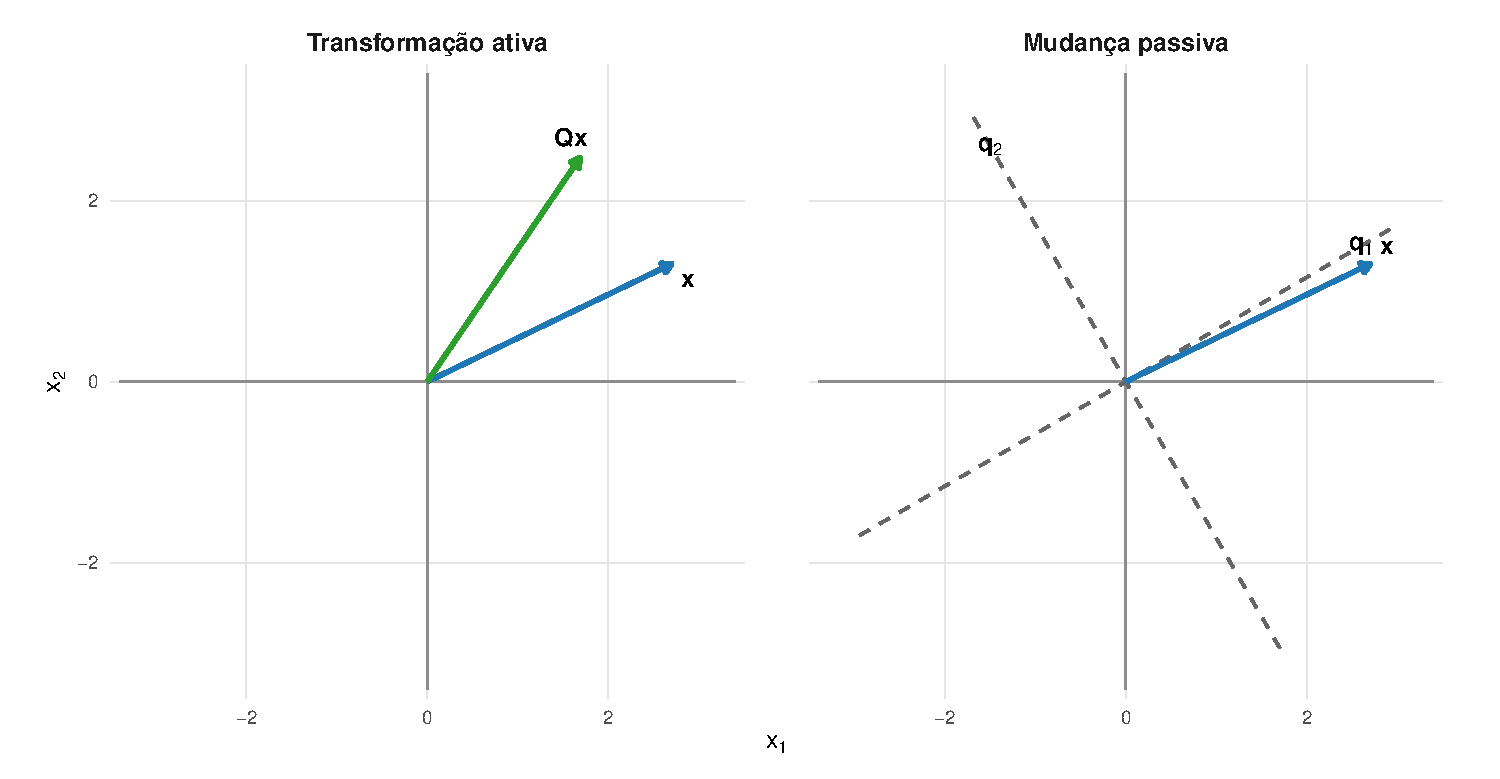
\includegraphics[keepaspectratio]{mod_1_transformacoes_files/figure-pdf/fig-ativa-passiva-1.pdf}}

}

\caption{\label{fig-ativa-passiva}Comparação entre uma transformação
ativa e uma mudança passiva de coordenadas.}

\end{figure}%

No primeiro painel, os eixos permanecem fixos e \(\mathbf{x}\) é
transformado em \(\mathbf{Q}\mathbf{x}\). No segundo, o vetor permanece
fixo e os novos eixos são definidos por \(\mathbf{q}_1\) e
\(\mathbf{q}_2\).

\subsection{Mudança de coordenadas de uma matriz de
dados}\label{mudanuxe7a-de-coordenadas-de-uma-matriz-de-dados}

Considere

\[
\mathbf{X}
\in
\mathbb{R}^{n\times p},
\]

com as observações organizadas nas linhas, e uma base ortonormal cujos
vetores estão nas colunas de \(\mathbf{Q}\).

As coordenadas da \(i\)-ésima observação na nova base são

\[
\mathbf{z}_i
=
\mathbf{Q}^{\top}\mathbf{x}_i.
\]

Transpondo,

\[
\mathbf{z}_i^{\top}
=
\mathbf{x}_i^{\top}\mathbf{Q}.
\]

Portanto, a matriz de novas coordenadas é

\[
\mathbf{Z}
=
\mathbf{X}\mathbf{Q}.
\]

Essa expressão deve ser distinguida da transformação ativa por
\(\mathbf{Q}\), que produz

\[
\mathbf{Y}
=
\mathbf{X}\mathbf{Q}^{\top}.
\]

A Tabela~\ref{tbl-ativa-passiva} resume as duas operações.

\begin{longtable}[]{@{}
  >{\raggedright\arraybackslash}p{(\linewidth - 4\tabcolsep) * \real{0.3333}}
  >{\raggedright\arraybackslash}p{(\linewidth - 4\tabcolsep) * \real{0.3333}}
  >{\raggedright\arraybackslash}p{(\linewidth - 4\tabcolsep) * \real{0.3333}}@{}}
\caption{Transformação ativa e mudança passiva para uma base
ortonormal.}\label{tbl-ativa-passiva}\tabularnewline
\toprule\noalign{}
\begin{minipage}[b]{\linewidth}\raggedright
Operação
\end{minipage} & \begin{minipage}[b]{\linewidth}\raggedright
Vetor-coluna
\end{minipage} & \begin{minipage}[b]{\linewidth}\raggedright
Matriz de dados
\end{minipage} \\
\midrule\noalign{}
\endfirsthead
\toprule\noalign{}
\begin{minipage}[b]{\linewidth}\raggedright
Operação
\end{minipage} & \begin{minipage}[b]{\linewidth}\raggedright
Vetor-coluna
\end{minipage} & \begin{minipage}[b]{\linewidth}\raggedright
Matriz de dados
\end{minipage} \\
\midrule\noalign{}
\endhead
\bottomrule\noalign{}
\endlastfoot
Transformação ativa por \(\mathbf{Q}\) &
\(\mathbf{y}=\mathbf{Q}\mathbf{x}\) &
\(\mathbf{Y}=\mathbf{X}\mathbf{Q}^{\top}\) \\
Mudança passiva para a base formada pelas colunas de \(\mathbf{Q}\) &
\(\mathbf{z}=\mathbf{Q}^{\top}\mathbf{x}\) &
\(\mathbf{Z}=\mathbf{X}\mathbf{Q}\) \\
\end{longtable}

Na transformação ativa, a configuração é modificada em relação a um
sistema de coordenadas fixo. Na mudança passiva, a configuração
permanece a mesma e cada observação passa a ser descrita pelas
coordenadas em uma nova base.

\section{Transformações afins e
pré-processamento}\label{transformauxe7uxf5es-afins-e-pruxe9-processamento}

Toda transformação linear mantém o vetor nulo fixo:

\[
T(\mathbf{0})
=
\mathbf{0}.
\]

Operações que incluem um deslocamento constante não satisfazem essa
propriedade. Elas pertencem a uma classe mais ampla, formada pelas
transformações afins.

\begin{definition}[Transformação
afim]\protect\hypertarget{def-transformacao-afim}{}\label{def-transformacao-afim}

Uma aplicação

\[
T:
\mathbb{R}^p
\longrightarrow
\mathbb{R}^q
\]

é uma \textbf{transformação afim} quando pode ser escrita como

\[
T(\mathbf{x})
=
\mathbf{A}\mathbf{x}
+
\mathbf{b},
\]

em que

\[
\mathbf{A}
\in
\mathbb{R}^{q\times p}
\]

e

\[
\mathbf{b}
\in
\mathbb{R}^q.
\]

\end{definition}

A matriz \(\mathbf{A}\) determina a parte linear da transformação,
enquanto \(\mathbf{b}\) determina o deslocamento.

Quando

\[
\mathbf{b}
=
\mathbf{0},
\]

a transformação afim reduz-se a uma transformação linear.

Quando

\[
\mathbf{b}
\neq
\mathbf{0},
\]

tem-se

\[
T(\mathbf{0})
=
\mathbf{b}
\neq
\mathbf{0},
\]

e a transformação não é linear.

\subsection{Translação}\label{translauxe7uxe3o}

A translação é o caso particular

\[
T(\mathbf{x})
=
\mathbf{x}
+
\mathbf{b}.
\]

Todos os pontos são deslocados pelo mesmo vetor \(\mathbf{b}\).

Para dois vetores \(\mathbf{x}_i\) e \(\mathbf{x}_j\),

\[
\begin{aligned}
T(\mathbf{x}_i)
-
T(\mathbf{x}_j)
&=
\left(
\mathbf{x}_i+\mathbf{b}
\right)
-
\left(
\mathbf{x}_j+\mathbf{b}
\right)\\
&=
\mathbf{x}_i-\mathbf{x}_j.
\end{aligned}
\]

Consequentemente,

\[
\|
T(\mathbf{x}_i)
-
T(\mathbf{x}_j)
\|
=
\|
\mathbf{x}_i-\mathbf{x}_j
\|.
\]

A translação preserva:

\begin{itemize}
\tightlist
\item
  diferenças entre os pontos;
\item
  distâncias;
\item
  ângulos entre segmentos;
\item
  forma;
\item
  áreas e volumes.
\end{itemize}

Ela modifica apenas a posição da configuração em relação à origem.

\subsection{Transformação afim de uma matriz de
dados}\label{transformauxe7uxe3o-afim-de-uma-matriz-de-dados}

Considere uma transformação afim aplicada a cada observação:

\[
\mathbf{y}_i
=
\mathbf{A}\mathbf{x}_i
+
\mathbf{b}.
\]

Se as observações estão organizadas nas linhas de

\[
\mathbf{X}
\in
\mathbb{R}^{n\times p},
\]

a matriz transformada é

\[
\mathbf{Y}
=
\mathbf{X}\mathbf{A}^{\top}
+
\mathbf{1}_n\mathbf{b}^{\top},
\]

em que

\[
\mathbf{1}_n
=
\begin{bmatrix}
1\\
\vdots\\
1
\end{bmatrix}
\in
\mathbb{R}^n.
\]

A matriz

\[
\mathbf{1}_n\mathbf{b}^{\top}
\]

possui dimensão \(n\times q\) e contém \(n\) linhas iguais a
\(\mathbf{b}^{\top}\). Assim, o mesmo deslocamento é acrescentado a
todas as observações.

As dimensões da transformação são

\[
\underbrace{\mathbf{X}}_{n\times p}
\underbrace{\mathbf{A}^{\top}}_{p\times q}
+
\underbrace{\mathbf{1}_n}_{n\times 1}
\underbrace{\mathbf{b}^{\top}}_{1\times q}
=
\underbrace{\mathbf{Y}}_{n\times q}.
\]

No caso de uma translação pura,

\[
\mathbf{A}
=
\mathbf{I}_p,
\]

e

\[
\mathbf{Y}
=
\mathbf{X}
+
\mathbf{1}_n\mathbf{b}^{\top}.
\]

\subsection{Centralização}\label{centralizauxe7uxe3o}

A centralização desloca uma configuração para que um vetor de
localização coincida com a origem.

Para um vetor fixo

\[
\mathbf{m}
\in
\mathbb{R}^p,
\]

define-se

\[
\mathbf{x}_c
=
\mathbf{x}
-
\mathbf{m}.
\]

Essa operação é afim:

\[
T(\mathbf{x})
=
\mathbf{I}_p\mathbf{x}
-
\mathbf{m}.
\]

Quando

\[
\mathbf{m}
\neq
\mathbf{0},
\]

ela não é linear, pois

\[
T(\mathbf{0})
=
-\mathbf{m}.
\]

Para uma matriz de dados,

\[
\mathbf{X}
=
\begin{bmatrix}
\mathbf{x}_1^{\top}\\
\vdots\\
\mathbf{x}_n^{\top}
\end{bmatrix},
\]

a centralização por \(\mathbf{m}\) é

\[
\mathbf{X}_c
=
\mathbf{X}
-
\mathbf{1}_n\mathbf{m}^{\top}.
\]

Quando o vetor de localização é a média amostral,

\[
\bar{\mathbf{x}}
=
\frac{1}{n}
\sum_{i=1}^{n}
\mathbf{x}_i,
\]

tem-se

\[
\mathbf{X}_c
=
\mathbf{X}
-
\mathbf{1}_n\bar{\mathbf{x}}^{\top}.
\]

Retomando a matriz de centralização,

\[
\mathbf{H}_n
=
\mathbf{I}_n
-
\frac{1}{n}
\mathbf{1}_n\mathbf{1}_n^{\top},
\]

a matriz centralizada pode ser escrita como

\[\mathbf{X}_c=\mathbf{H}_n\mathbf{X}.\]

De fato,

\[
\begin{aligned}
\mathbf{H}_n\mathbf{X}
&=
\left(
\mathbf{I}_n
-
\frac{1}{n}
\mathbf{1}_n\mathbf{1}_n^{\top}
\right)
\mathbf{X}\\
&=
\mathbf{X}
-
\mathbf{1}_n
\left(
\frac{1}{n}
\mathbf{1}_n^{\top}\mathbf{X}
\right)\\
&=
\mathbf{X}
-
\mathbf{1}_n\bar{\mathbf{x}}^{\top}.
\end{aligned}
\]

A centralização de cada observação em torno de um vetor fixo é uma
transformação afim. Em contraste, a aplicação

\[
\mathbf{X}
\longmapsto
\mathbf{H}_n\mathbf{X}
\]

sobre o espaço das matrizes de dados é linear, pois \(\mathbf{H}_n\) é
uma matriz fixa.

Além disso,

\[
\mathbf{H}_n
=
\mathbf{H}_n^{\top}
\]

e

\[
\mathbf{H}_n^2
=
\mathbf{H}_n.
\]

Portanto, \(\mathbf{H}_n\) é uma matriz de projeção ortogonal. Como

\[\mathbf{H}_n\mathbf{1}_n=\mathbf{0},\]

seu núcleo é

\[
\mathcal{N}(\mathbf{H}_n)
=
\operatorname{span}\{\mathbf{1}_n\},
\]

e sua imagem é o subespaço

\[
\mathcal{C}(\mathbf{H}_n)
=
\left\{
\mathbf{z}\in\mathbb{R}^n:
\mathbf{1}_n^{\top}\mathbf{z}=0
\right\}
=
\operatorname{span}\{\mathbf{1}_n\}^{\perp}.
\]

Assim, multiplicar uma variável observada por \(\mathbf{H}_n\) equivale
a projetá-la ortogonalmente sobre o subespaço dos vetores cujas
componentes somam zero.

Como \(\mathbf{H}_n\) é simétrica e

\[\mathbf{H}_n\mathbf{1}_n=\mathbf{0},\]

tem-se também

\[\mathbf{1}_n^{\top}\mathbf{H}_n=\mathbf{0}^{\top}.\]

Consequentemente,

\[
\mathbf{1}_n^{\top}\mathbf{X}_c
=
\mathbf{1}_n^{\top}\mathbf{H}_n\mathbf{X}
=
\mathbf{0}^{\top}.
\]

Portanto, cada coluna de \(\mathbf{X}_c\) possui média igual a zero.

\begin{proposition}[Preservação das distâncias pela
centralização]\protect\hypertarget{prp-centralizacao-preserva-distancias}{}\label{prp-centralizacao-preserva-distancias}

Se

\[
\mathbf{x}_{ci}
=
\mathbf{x}_i-\mathbf{m}
\]

e

\[
\mathbf{x}_{cj}
=
\mathbf{x}_j-\mathbf{m},
\]

então

\[
\|
\mathbf{x}_{ci}
-
\mathbf{x}_{cj}
\|
=
\|
\mathbf{x}_i
-
\mathbf{x}_j
\|.
\]

\end{proposition}

\begin{proof}
Tem-se

\[
\begin{aligned}
\mathbf{x}_{ci}
-
\mathbf{x}_{cj}
&=
\left(
\mathbf{x}_i-\mathbf{m}
\right)
-
\left(
\mathbf{x}_j-\mathbf{m}
\right)\\
&=
\mathbf{x}_i-\mathbf{x}_j.
\end{aligned}
\]

Logo, as duas diferenças possuem a mesma norma.
\end{proof}

A centralização modifica a posição da nuvem em relação à origem, mas
preserva sua configuração interna.

\subsection{Escalonamento das
variáveis}\label{escalonamento-das-variuxe1veis}

Considere uma matriz diagonal

\[
\mathbf{L}
=
\operatorname{diag}
\left(
\ell_1,\ldots,\ell_p
\right),
\]

com

\[
\ell_j>0,
\qquad
j=1,\ldots,p.
\]

A transformação

\[
\mathbf{y}
=
\mathbf{L}^{-1}\mathbf{x}
\]

divide cada coordenada por sua escala correspondente:

\[
y_j
=
\frac{x_j}{\ell_j}.
\]

Essa operação é linear e, para uma matriz de dados, assume a forma

\[
\mathbf{Y}
=
\mathbf{X}\mathbf{L}^{-1}.
\]

A multiplicação ocorre à direita porque as variáveis ocupam as colunas
de \(\mathbf{X}\).

Quando as escalas são diferentes, o escalonamento modifica, em geral,
distâncias e ângulos. Alguns pares particulares de vetores podem manter
sua relação angular, mas a geometria euclidiana não é preservada para
todos os vetores. Para duas observações,

\[
\begin{aligned}
\|
\mathbf{L}^{-1}\mathbf{x}_i
-
\mathbf{L}^{-1}\mathbf{x}_j
\|^2
&=
\left(
\mathbf{x}_i-\mathbf{x}_j
\right)^{\top}
\mathbf{L}^{-2}
\left(
\mathbf{x}_i-\mathbf{x}_j
\right).
\end{aligned}
\]

O escalonamento induz, no espaço original, a geometria determinada pela
matriz positiva definida

\[\mathbf{L}^{-2}.\]

Variáveis associadas a escalas menores recebem maior peso nas distâncias
transformadas. Quando todas as escalas são iguais, isto é,

\[\mathbf{L}=\ell\mathbf{I}_p,\]

o escalonamento é uniforme: todas as distâncias são multiplicadas pelo
mesmo fator \(1/\ell\) e os ângulos são preservados.

\subsection{Padronização}\label{padronizauxe7uxe3o}

A padronização combina centralização e escalonamento.

Para um vetor de localização \(\mathbf{m}\) e uma matriz diagonal de
escalas positivas \(\mathbf{L}\), define-se

\[
\mathbf{z}
=
\mathbf{L}^{-1}
\left(
\mathbf{x}-\mathbf{m}
\right).
\]

Essa expressão pode ser reorganizada como

\[
\mathbf{z}
=
\mathbf{L}^{-1}\mathbf{x}
-
\mathbf{L}^{-1}\mathbf{m}.
\]

Portanto, a padronização é uma transformação afim com

\[
\mathbf{A}
=
\mathbf{L}^{-1}
\]

e

\[
\mathbf{b}
=
-\mathbf{L}^{-1}\mathbf{m}.
\]

Para uma matriz de dados,

\[
\mathbf{Z}
=
\left(
\mathbf{X}
-
\mathbf{1}_n\mathbf{m}^{\top}
\right)
\mathbf{L}^{-1}.
\]

Quando \(\mathbf{m}=\bar{\mathbf{x}}\) e os elementos diagonais de
\(\mathbf{L}\) são os desvios-padrão amostrais, cada coluna de
\(\mathbf{Z}\) possui média zero e desvio-padrão igual a 1, desde que
todas as variáveis apresentem desvio-padrão amostral positivo.

A interpretação da padronização como transformação afim considera
\(\mathbf{m}\) e \(\mathbf{L}\) fixados. Quando o vetor de médias e os
desvios-padrão são calculados a partir da própria matriz de dados
\(\mathbf{X}\), esses elementos passam a depender dos dados. Nesse caso,
para os valores calculados de \(\mathbf{m}\) e \(\mathbf{L}\), cada
observação é submetida à transformação afim

\[
\mathbf{x}
\longmapsto
\mathbf{L}^{-1}
\left(
\mathbf{x}-\mathbf{m}
\right),
\]

mas a operação completa que associa a matriz original \(\mathbf{X}\) à
matriz padronizada \(\mathbf{Z}\) é dependente dos dados e não
constitui, globalmente, uma transformação afim de \(\mathbf{X}\).

Para duas observações padronizadas,

\[
\begin{aligned}
\mathbf{z}_i-\mathbf{z}_j
&=
\mathbf{L}^{-1}
\left(
\mathbf{x}_i-\mathbf{m}
\right)
-
\mathbf{L}^{-1}
\left(
\mathbf{x}_j-\mathbf{m}
\right)\\
&=
\mathbf{L}^{-1}
\left(
\mathbf{x}_i-\mathbf{x}_j
\right).
\end{aligned}
\]

Logo,

\[
\|
\mathbf{z}_i-\mathbf{z}_j
\|^2
=
\left(
\mathbf{x}_i-\mathbf{x}_j
\right)^{\top}
\mathbf{L}^{-2}
\left(
\mathbf{x}_i-\mathbf{x}_j
\right).
\]

A translação associada à centralização não altera as diferenças entre
observações. A alteração da geometria decorre do escalonamento.

\subsection{Ordem entre centralização e
escalonamento}\label{ordem-entre-centralizauxe7uxe3o-e-escalonamento}

A padronização usual é

\[
\mathbf{z}
=
\mathbf{L}^{-1}
\left(
\mathbf{x}-\mathbf{m}
\right).
\]

Se o escalonamento for aplicado primeiro,

\[
\mathbf{y}
=
\mathbf{L}^{-1}\mathbf{x},
\]

o vetor de localização também deve ser expresso na nova escala:

\[
\mathbf{L}^{-1}\mathbf{m}.
\]

Assim,

\[
\mathbf{z}
=
\mathbf{y}
-
\mathbf{L}^{-1}\mathbf{m}.
\]

As duas sequências produzem o mesmo resultado quando o vetor de
centralização é transformado juntamente com os dados.

\subsection{Composição e inversão de transformações
afins}\label{composiuxe7uxe3o-e-inversuxe3o-de-transformauxe7uxf5es-afins}

Considere

\[
T_1(\mathbf{x})
=
\mathbf{A}\mathbf{x}
+
\mathbf{b}
\]

e

\[
T_2(\mathbf{y})
=
\mathbf{C}\mathbf{y}
+
\mathbf{d}.
\]

A composição é

\[
\begin{aligned}
T_2
\left(
T_1(\mathbf{x})
\right)
&=
\mathbf{C}
\left(
\mathbf{A}\mathbf{x}
+
\mathbf{b}
\right)
+
\mathbf{d}\\
&=
\mathbf{C}\mathbf{A}\mathbf{x}
+
\mathbf{C}\mathbf{b}
+
\mathbf{d}.
\end{aligned}
\]

Portanto,

\[
\left(
T_2\circ T_1
\right)
(\mathbf{x})
=
\mathbf{C}\mathbf{A}\mathbf{x}
+
\left(
\mathbf{C}\mathbf{b}
+
\mathbf{d}
\right).
\]

A composição de transformações afins também é afim.

Considere agora

\[
\mathbf{y}
=
\mathbf{A}\mathbf{x}
+
\mathbf{b},
\]

com \(\mathbf{A}\) quadrada e invertível. Subtraindo \(\mathbf{b}\) e
multiplicando por \(\mathbf{A}^{-1}\),

\[
\mathbf{x}
=
\mathbf{A}^{-1}
\left(
\mathbf{y}-\mathbf{b}
\right).
\]

A transformação inversa é

\[
T^{-1}(\mathbf{y})
=
\mathbf{A}^{-1}\mathbf{y}
-
\mathbf{A}^{-1}\mathbf{b}.
\]

Uma transformação afim de \(\mathbb{R}^p\) em \(\mathbb{R}^p\) é
invertível se, e somente se, sua parte linear \(\mathbf{A}\) é
invertível.

\subsection{Comparação das operações de
pré-processamento}\label{comparauxe7uxe3o-das-operauxe7uxf5es-de-pruxe9-processamento}

A Figura~\ref{fig-transformacoes-afins} compara centralização,
escalonamento e padronização de uma mesma nuvem de pontos. O mesmo vetor
de escalas é utilizado no escalonamento e na padronização, permitindo
separar visualmente o efeito da alteração de escala do efeito da
centralização.

\begin{figure}

\centering{

\pandocbounded{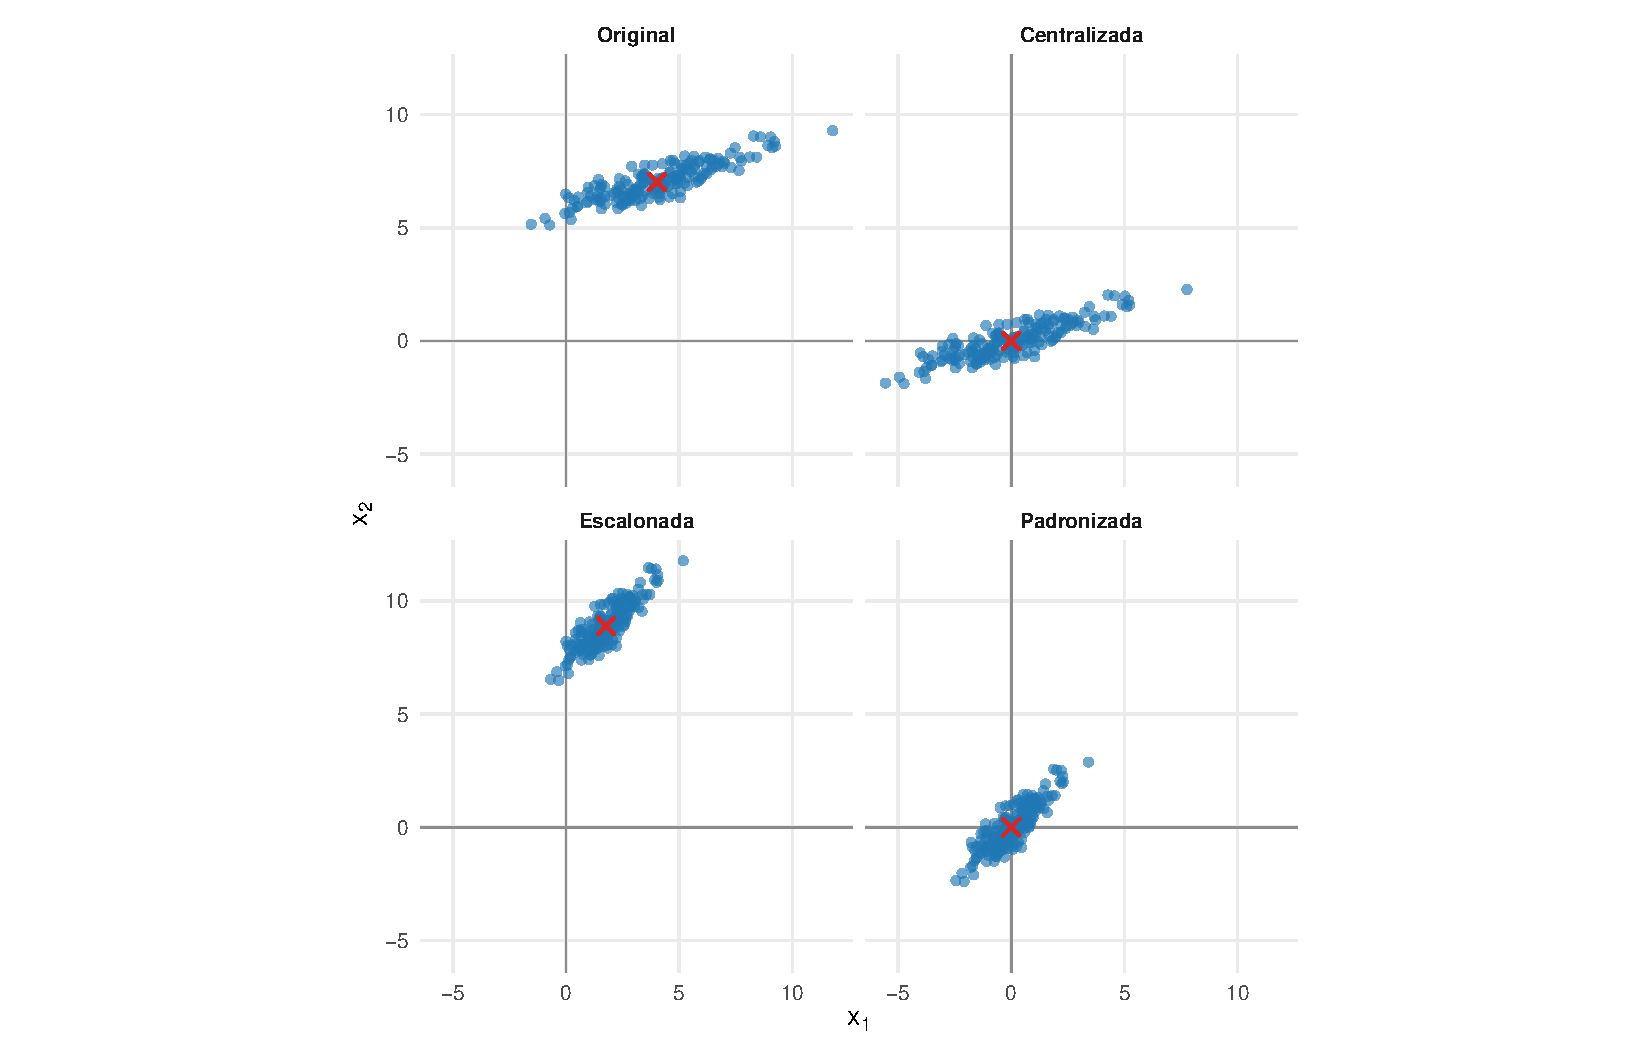
\includegraphics[keepaspectratio]{mod_1_transformacoes_files/figure-pdf/fig-transformacoes-afins-1.pdf}}

}

\caption{\label{fig-transformacoes-afins}Efeito da centralização, do
escalonamento e da padronização sobre uma mesma configuração de dados.}

\end{figure}%

A centralização desloca a nuvem para que sua média coincida com a
origem, sem modificar as diferenças nem as distâncias entre as
observações. O escalonamento altera as unidades das coordenadas e, em
geral, modifica comprimentos, distâncias e ângulos. A padronização
combina esses dois efeitos: centraliza a nuvem e reescala suas
coordenadas.

A Tabela~\ref{tbl-lineares-afins} resume as diferenças entre as
transformações estudadas nesta seção.

\begin{longtable}[]{@{}
  >{\raggedright\arraybackslash}p{(\linewidth - 6\tabcolsep) * \real{0.2222}}
  >{\raggedright\arraybackslash}p{(\linewidth - 6\tabcolsep) * \real{0.2222}}
  >{\centering\arraybackslash}p{(\linewidth - 6\tabcolsep) * \real{0.2778}}
  >{\centering\arraybackslash}p{(\linewidth - 6\tabcolsep) * \real{0.2778}}@{}}
\caption{Comparação entre transformações lineares, transformações afins
e operações de
pré-processamento.}\label{tbl-lineares-afins}\tabularnewline
\toprule\noalign{}
\begin{minipage}[b]{\linewidth}\raggedright
Operação
\end{minipage} & \begin{minipage}[b]{\linewidth}\raggedright
Expressão para um vetor
\end{minipage} & \begin{minipage}[b]{\linewidth}\centering
Linear como função de \(\mathbf{x}\)?
\end{minipage} & \begin{minipage}[b]{\linewidth}\centering
Mantém a origem fixa?
\end{minipage} \\
\midrule\noalign{}
\endfirsthead
\toprule\noalign{}
\begin{minipage}[b]{\linewidth}\raggedright
Operação
\end{minipage} & \begin{minipage}[b]{\linewidth}\raggedright
Expressão para um vetor
\end{minipage} & \begin{minipage}[b]{\linewidth}\centering
Linear como função de \(\mathbf{x}\)?
\end{minipage} & \begin{minipage}[b]{\linewidth}\centering
Mantém a origem fixa?
\end{minipage} \\
\midrule\noalign{}
\endhead
\bottomrule\noalign{}
\endlastfoot
Transformação linear & \(\mathbf{A}\mathbf{x}\) & Sim & Sim \\
Translação & \(\mathbf{x}+\mathbf{b}\) & Não, se
\(\mathbf{b}\neq\mathbf{0}\) & Não \\
Transformação afim & \(\mathbf{A}\mathbf{x}+\mathbf{b}\) & Não, em geral
& Não, em geral \\
Centralização & \(\mathbf{x}-\mathbf{m}\) & Não, se
\(\mathbf{m}\neq\mathbf{0}\) & Não \\
Escalonamento & \(\mathbf{L}^{-1}\mathbf{x}\) & Sim & Sim \\
Padronização & \(\mathbf{L}^{-1}(\mathbf{x}-\mathbf{m})\) & Não, em
geral & Não, em geral \\
\end{longtable}

Transformações lineares podem modificar direção, escala ou dimensão, mas
mantêm necessariamente a origem fixa. Transformações afins acrescentam a
possibilidade de deslocar a configuração. A centralização e a
padronização pertencem a essa segunda classe quando consideradas como
operações sobre uma observação individual e para parâmetros de
localização e escala fixados. Quando a centralização de uma matriz de
dados é escrita como \(\mathbf{X}\mapsto\mathbf{H}_n\mathbf{X}\), a
operação é linear no espaço das matrizes.

\section{Síntese do capítulo}\label{suxedntese-do-capuxedtulo-3}

Uma transformação linear preserva combinações lineares. Para uma
transformação

\[T:V\longrightarrow W,\]

tem-se

\[
T(\alpha\mathbf{u}+\beta\mathbf{v})
=
\alpha T(\mathbf{u})
+
\beta T(\mathbf{v}).
\]

Essa propriedade implica, entre outras consequências,

\[T(\mathbf{0})=\mathbf{0},\]

e permite determinar uma transformação linear a partir de sua ação sobre
uma base do domínio.

Fixadas as bases do domínio e do contradomínio, uma transformação linear
possui uma representação matricial única. Em particular, nas bases
canônicas, uma transformação

\[
T_{\mathbf{A}}:
\mathbb{R}^p
\longrightarrow
\mathbb{R}^q
\]

é representada por

\[
T_{\mathbf{A}}(\mathbf{x})
=
\mathbf{A}\mathbf{x},
\qquad
\mathbf{A}\in\mathbb{R}^{q\times p}.
\]

Quando as observações ocupam as linhas de uma matriz de dados

\[\mathbf{X}\in\mathbb{R}^{n\times p},\]

a transformação simultânea das observações é

\[\mathbf{Y}=\mathbf{X}\mathbf{A}^{\top}.\]

Cada linha de \(\mathbf{Y}\) representa uma observação transformada,
enquanto cada coluna corresponde a uma combinação linear das variáveis
originais.

A matriz associada à transformação permite relacionar os conceitos
desenvolvidos neste capítulo aos espaços fundamentais estudados
anteriormente:

\[
\ker(T_{\mathbf{A}})
=
\mathcal{N}(\mathbf{A})
\]

e

\[
\operatorname{Im}(T_{\mathbf{A}})
=
\mathcal{C}(\mathbf{A}).
\]

Assim, o núcleo reúne os vetores eliminados pela transformação, enquanto
a imagem contém todos os vetores que podem ser produzidos por ela. Pelo
teorema posto-nulidade,

\[
\dim\ker(T_{\mathbf{A}})
+
\dim\operatorname{Im}(T_{\mathbf{A}})
=
p,
\]

ou, equivalentemente,

\[
\dim\mathcal{N}(\mathbf{A})
+
\operatorname{posto}(\mathbf{A})
=
p.
\]

O posto é, portanto, a dimensão da imagem da transformação. Quando o
núcleo contém vetores não nulos, diferentes vetores do domínio podem
possuir a mesma imagem e ocorre perda de informação.

Para uma transformação quadrada, as condições

\[
\ker(T_{\mathbf{A}})=\{\mathbf{0}\},
\]

\[
\operatorname{Im}(T_{\mathbf{A}})=\mathbb{R}^p,
\]

\[
\operatorname{posto}(\mathbf{A})=p,
\]

\[
\det(\mathbf{A})\neq0
\]

e a existência de \(\mathbf{A}^{-1}\) são equivalentes.

A composição de transformações corresponde ao produto de suas matrizes.
Se \(T_1\) é representada por \(\mathbf{A}_1\) e \(T_2\) por
\(\mathbf{A}_2\), então

\[
[T_2\circ T_1]
=
\mathbf{A}_2\mathbf{A}_1.
\]

A matriz situada à direita atua primeiro. Como o produto matricial não é
comutativo, a ordem das transformações pode alterar o resultado.

As transformações geométricas estudadas ilustram diferentes efeitos
possíveis sobre uma configuração. Rotações e reflexões são
transformações ortogonais e preservam a geometria euclidiana.
Escalonamentos alteram as escalas das direções coordenadas;
cisalhamentos modificam, em geral, ângulos e comprimentos; projeções
eliminam componentes pertencentes ao complemento do subespaço sobre o
qual se projeta.

Para uma transformação quadrada,

\[|\det(\mathbf{A})|\]

representa o fator de alteração do volume \(p\)-dimensional. Quando
\(\det(\mathbf{A})\neq0\), seu sinal informa também o efeito sobre a
orientação: valores positivos preservam a orientação e valores negativos
a invertem. Se

\[\det(\mathbf{A})=0,\]

a transformação reduz a dimensão e o volume \(p\)-dimensional da imagem
é igual a zero.

As transformações ortogonais são caracterizadas por

\[\mathbf{Q}^{\top}\mathbf{Q}=\mathbf{I}_p.\]

Elas preservam produtos internos e, consequentemente, normas,
distâncias, ângulos e ortogonalidade. Além disso,

\[\mathbf{Q}^{-1}=\mathbf{Q}^{\top}\]

e

\[\det(\mathbf{Q})\in\{-1,1\},\]

de modo que também preservam volumes \(p\)-dimensionais.

As colunas de uma matriz ortogonal formam uma base ortonormal e
satisfazem

\[\mathbf{q}_i^{\top}\mathbf{q}_j=\delta_{ij}.\]

Essa propriedade estabelece a ligação entre transformações ortogonais e
sistemas de coordenadas ortonormais.

Se

\[
\mathcal{B}
=
\{
\mathbf{b}_1,\ldots,\mathbf{b}_p
\}
\]

é uma base de \(\mathbb{R}^p\) e

\[
\mathbf{B}
=
\begin{bmatrix}
\mathbf{b}_1&
\cdots&
\mathbf{b}_p
\end{bmatrix},
\]

então

\[\mathbf{x}=\mathbf{B}[\mathbf{x}]_{\mathcal{B}}\]

e

\[[\mathbf{x}]_{\mathcal{B}}=\mathbf{B}^{-1}\mathbf{x}.\]

Para duas bases \(\mathcal{B}\) e \(\mathcal{C}\), com matrizes
\(\mathbf{B}\) e \(\mathbf{C}\), respectivamente, a conversão das
coordenadas de \(\mathcal{B}\) para \(\mathcal{C}\) é

\[
[\mathbf{x}]_{\mathcal{C}}
=
\mathbf{C}^{-1}
\mathbf{B}
[\mathbf{x}]_{\mathcal{B}}.
\]

Se uma transformação é representada nas bases canônicas por
\(\mathbf{A}\), sua matriz em relação à base \(\mathcal{B}\) do domínio
e à base \(\mathcal{C}\) do contradomínio é

\[
[T]_{\mathcal{C}\leftarrow\mathcal{B}}
=
\mathbf{C}^{-1}
\mathbf{A}
\mathbf{B}.
\]

Quando a mesma base é utilizada no domínio e no contradomínio,

\[
\mathbf{A}_{\mathcal{B}}
=
\mathbf{B}^{-1}
\mathbf{A}
\mathbf{B},
\]

de modo que as duas matrizes são semelhantes e representam o mesmo
operador em sistemas de coordenadas distintos.

A transformação ativa e a mudança passiva de coordenadas devem ser
diferenciadas. Se \(\mathbf{Q}\) é ortogonal, na transformação ativa,

\[\mathbf{y}=\mathbf{Q}\mathbf{x},\]

enquanto, na mudança passiva para a base formada pelas colunas de
\(\mathbf{Q}\),

\[
[\mathbf{x}]_{\mathcal{B}}
=
\mathbf{Q}^{\top}\mathbf{x}.
\]

Na primeira situação, o vetor é transformado em relação a eixos fixos.
Na segunda, o vetor geométrico permanece o mesmo e apenas sua
representação em coordenadas é alterada.

As transformações afins generalizam as transformações lineares por meio
da inclusão de uma translação:

\[T(\mathbf{x})=\mathbf{A}\mathbf{x}+\mathbf{b}.\]

A centralização de uma observação em torno de um vetor fixo é uma
transformação afim, enquanto o escalonamento é uma transformação linear
diagonal. A padronização combina essas duas operações.

Para uma matriz de dados, a centralização pela média amostral pode ser
escrita como

\[\mathbf{X}_c=\mathbf{H}_n\mathbf{X},\]

em que

\[
\mathbf{H}_n
=
\mathbf{I}_n
-
\frac{1}{n}
\mathbf{1}_n\mathbf{1}_n^{\top}.
\]

Como

\[\mathbf{H}_n^{\top}=\mathbf{H}_n\]

e

\[\mathbf{H}_n^2=\mathbf{H}_n,\]

a matriz \(\mathbf{H}_n\) é uma matriz de projeção ortogonal. Sua imagem
é

\[
\mathcal{C}(\mathbf{H}_n)
=
\operatorname{span}\{\mathbf{1}_n\}^{\perp},
\]

o subespaço dos vetores cujas componentes somam zero.

A Tabela~\ref{tbl-sintese-transformacoes} reúne algumas das principais
expressões desenvolvidas no capítulo.

\begin{longtable}[]{@{}
  >{\raggedright\arraybackslash}p{(\linewidth - 4\tabcolsep) * \real{0.3333}}
  >{\raggedright\arraybackslash}p{(\linewidth - 4\tabcolsep) * \real{0.3333}}
  >{\raggedright\arraybackslash}p{(\linewidth - 4\tabcolsep) * \real{0.3333}}@{}}
\caption{Síntese das transformações desenvolvidas no
capítulo.}\label{tbl-sintese-transformacoes}\tabularnewline
\toprule\noalign{}
\begin{minipage}[b]{\linewidth}\raggedright
Objeto ou operação
\end{minipage} & \begin{minipage}[b]{\linewidth}\raggedright
Expressão
\end{minipage} & \begin{minipage}[b]{\linewidth}\raggedright
Interpretação
\end{minipage} \\
\midrule\noalign{}
\endfirsthead
\toprule\noalign{}
\begin{minipage}[b]{\linewidth}\raggedright
Objeto ou operação
\end{minipage} & \begin{minipage}[b]{\linewidth}\raggedright
Expressão
\end{minipage} & \begin{minipage}[b]{\linewidth}\raggedright
Interpretação
\end{minipage} \\
\midrule\noalign{}
\endhead
\bottomrule\noalign{}
\endlastfoot
Transformação linear &
\(T_{\mathbf{A}}(\mathbf{x})=\mathbf{A}\mathbf{x}\) & Preserva
combinações lineares \\
Transformação dos dados & \(\mathbf{Y}=\mathbf{X}\mathbf{A}^{\top}\) &
Transforma simultaneamente as observações \\
Núcleo & \(\ker(T_{\mathbf{A}})=\mathcal{N}(\mathbf{A})\) & Reúne os
vetores enviados ao vetor nulo \\
Imagem & \(\operatorname{Im}(T_{\mathbf{A}})=\mathcal{C}(\mathbf{A})\) &
Reúne os vetores alcançados pela transformação \\
Composição &
\((T_2\circ T_1)(\mathbf{x})=\mathbf{A}_2\mathbf{A}_1\mathbf{x}\) &
Aplica \(T_1\) antes de \(T_2\) \\
Transformação inversa & \(\mathbf{x}=\mathbf{A}^{-1}\mathbf{y}\) &
Recupera o vetor original quando \(\mathbf{A}\) é invertível \\
Rotação & \(\mathbf{Q}_\theta\mathbf{x}\) & Preserva a geometria e a
orientação \\
Reflexão & \(\mathbf{F}\mathbf{x}\) & Preserva a geometria; seu efeito
sobre a orientação é determinado pelo determinante \\
Escalonamento & \(\mathbf{L}\mathbf{x}\) & Reescala direções
coordenadas \\
Cisalhamento & \(\mathbf{C}_{ij}(k)\mathbf{x}\) & Inclina a configuração
preservando volume no caso elementar \\
Projeção ortogonal & \(\mathbf{P}_{S}\mathbf{x}\) & Mantém a componente
em \(S\) e elimina a componente em \(S^{\perp}\) \\
Coordenadas em uma base &
\([\mathbf{x}]_{\mathcal{B}}=\mathbf{B}^{-1}\mathbf{x}\) & Representa o
mesmo vetor na base \(\mathcal{B}\) \\
Mudança de \(\mathcal{B}\) para \(\mathcal{C}\) &
\([\mathbf{x}]_{\mathcal{C}}=\mathbf{C}^{-1}\mathbf{B}[\mathbf{x}]_{\mathcal{B}}\)
& Converte coordenadas entre bases \\
Transformação em bases gerais &
\([T]_{\mathcal{C}\leftarrow\mathcal{B}}=\mathbf{C}^{-1}\mathbf{A}\mathbf{B}\)
& Representa a transformação nas bases escolhidas \\
Transformação afim & \(\mathbf{A}\mathbf{x}+\mathbf{b}\) & Combina
transformação linear e translação \\
Centralização dos dados & \(\mathbf{X}_c=\mathbf{H}_n\mathbf{X}\) &
Projeta cada variável no subespaço de média zero \\
Padronização & \(\mathbf{L}^{-1}(\mathbf{x}-\mathbf{m})\) & Ajusta
localização e escala \\
\end{longtable}

Ao final deste capítulo, o estudante deverá ser capaz de:

\begin{itemize}
\tightlist
\item
  reconhecer e verificar a linearidade de uma transformação;
\item
  construir a matriz de uma transformação a partir da imagem de uma
  base;
\item
  relacionar núcleo e imagem de uma transformação ao espaço nulo e ao
  espaço coluna da matriz associada;
\item
  interpretar posto, injetividade, sobrejetividade, bijetividade e perda
  de informação;
\item
  representar a composição e a inversão de transformações por operações
  matriciais;
\item
  interpretar geometricamente rotações, reflexões, escalonamentos,
  cisalhamentos e projeções;
\item
  relacionar o determinante à alteração de volume, à orientação e à
  redução de dimensão;
\item
  reconhecer transformações ortogonais e interpretar as propriedades
  geométricas que elas preservam;
\item
  converter coordenadas entre bases;
\item
  representar uma transformação linear em bases distintas do domínio e
  do contradomínio;
\item
  distinguir transformação ativa e mudança passiva de coordenadas;
\item
  interpretar transformações afins, centralização, escalonamento e
  padronização;
\item
  reconhecer a matriz de centralização como uma matriz de projeção
  ortogonal.
\end{itemize}

No próximo capítulo, serão estudadas direções especiais para as quais a
ação de uma transformação linear produz um múltiplo escalar do próprio
vetor,

\[\mathbf{A}\mathbf{v}=\lambda\mathbf{v}.\]

Essas direções conduzem aos conceitos de autovetores, autovalores,
autoespaços e decomposição espectral.

\chapter{Autovalores, autovetores e decomposição
espectral}\label{autovalores-autovetores-e-decomposiuxe7uxe3o-espectral}

No capítulo anterior, uma transformação linear foi representada por uma
matriz e interpretada como uma operação capaz de modificar direções,
comprimentos, ângulos e volumes. Quando o domínio e o contradomínio
coincidem, a transformação é um operador linear

\[
T_{\mathbf{A}}:
\mathbb{R}^p
\longrightarrow
\mathbb{R}^p,
\qquad
T_{\mathbf{A}}(\mathbf{x})
=
\mathbf{A}\mathbf{x},
\]

representado por uma matriz quadrada

\[
\mathbf{A}
\in
\mathbb{R}^{p\times p}.
\]

Vimos também que a matriz de um operador depende da base utilizada para
representá-lo. Uma mudança de base pode produzir uma matriz mais
simples, embora o operador linear permaneça o mesmo. Neste capítulo,
procuraremos bases especialmente adaptadas à ação do operador.

Algumas direções possuem um comportamento particularmente simples:
quando um vetor pertence a uma dessas direções, sua imagem permanece na
mesma reta que passa pela origem. A identificação dessas direções conduz
aos conceitos de autovalor, autovetor e autoespaço.

Quando existem autovetores linearmente independentes em número
suficiente, eles formam uma base na qual a matriz do operador é
diagonal. A diagonalização pode, portanto, ser interpretada como uma
mudança para um sistema de coordenadas em que a transformação atua
separadamente sobre cada direção da base.

Para matrizes simétricas reais, essa simplificação possui propriedades
adicionais: todos os autovalores são reais e existe uma base ortonormal
de autovetores. A decomposição resultante permitirá interpretar formas
quadráticas, matrizes positivas definidas, elipsoides, funções de
matrizes e problemas de otimização. Essas estruturas serão retomadas nos
capítulos de SVD, covariâncias e técnicas multivariadas.

\begin{tcolorbox}[enhanced jigsaw, colback=white, breakable, bottomrule=.15mm, left=2mm, arc=.35mm, rightrule=.15mm, colframe=quarto-callout-note-color-frame, toprule=.15mm, leftrule=.75mm, opacityback=0]

\vspace{-3mm}\textbf{Convenções de notação}\vspace{3mm}

Ao longo deste capítulo:

\begin{itemize}
\tightlist
\item
  \(\lambda\) representa um autovalor;
\item
  \(\mathbf{v}\) representa um autovetor;
\item
  \(\mathcal{E}_{\lambda}\) representa o autoespaço associado a
  \(\lambda\);
\item
  \(m_a(\lambda)\) e \(m_g(\lambda)\) representam, respectivamente, as
  multiplicidades algébrica e geométrica;
\item
  \(\mathcal{B}_{\mathbf{A}}\) representa uma base de autovetores de
  \(\mathbf{A}\), quando tal base existe;
\item
  \(\mathbf{B}_{\mathbf{A}}\) representa a matriz formada pelos vetores
  da base \(\mathcal{B}_{\mathbf{A}}\);
\item
  \(\boldsymbol{\Lambda}_{\mathbf{A}}\) representa a matriz diagonal dos
  autovalores correspondente à ordenação escolhida dos autovetores;
\item
  \(\mathbf{Q}_{\mathbf{A}}\) representa uma matriz ortogonal de
  autovetores quando \(\mathbf{A}\) é simétrica;
\item
  \(\boldsymbol{\Pi}_{\lambda}\) representa o projetor espectral
  associado ao autoespaço de \(\lambda\);
\item
  \(\mathcal{R}_{\mathbf{A}}(\mathbf{x})\) representa o quociente de
  Rayleigh.
\end{itemize}

Salvo indicação contrária, as interpretações geométricas serão
desenvolvidas em espaços vetoriais reais. Autovalores e autovetores
complexos serão considerados explicitamente quando necessário.

\end{tcolorbox}

\section{Direções invariantes, autovalores e
autoespaços}\label{direuxe7uxf5es-invariantes-autovalores-e-autoespauxe7os}

\begin{definition}[Subespaço
invariante]\protect\hypertarget{def-subespaco-invariante}{}\label{def-subespaco-invariante}

Considere

\[
\mathbf A
\in
\mathbb R^{p\times p}
\]

e um subespaço

\[
\mathcal W
\subseteq
\mathbb R^p.
\]

O subespaço \(\mathcal W\) é \textbf{invariante sob \(\mathbf A\)}
quando

\[
\mathbf A\mathbf w
\in
\mathcal W
\]

para todo

\[
\mathbf w
\in
\mathcal W.
\]

Isso significa que a multiplicação por \(\mathbf A\) transforma vetores
de \(\mathcal W\) em vetores que permanecem no próprio subespaço
\(\mathcal W\).

\end{definition}

Um caso particularmente importante ocorre quando o subespaço invariante
possui dimensão \(1\).

Seja

\[
\mathbf v
\in
\mathbb R^p,
\qquad
\mathbf v\neq\mathbf 0.
\]

O subespaço gerado por \(\mathbf v\) é

\[
\mathcal W
=
\operatorname{span}\{\mathbf v\}
=
\left\{
c\mathbf v:
c\in\mathbb R
\right\}.
\]

Como \(\mathbf v\neq\mathbf 0\), o conjunto \(\{\mathbf v\}\) é uma base
de \(\mathcal W\) e, portanto,

\[
\dim(\mathcal W)=1.
\]

Geometricamente, \(\mathcal W\) corresponde a uma reta que passa pela
origem e está contida em \(\mathbb R^p\).

Se \(\mathcal W\) é invariante sob \(\mathbf A\), então

\[
\mathbf A\mathbf v
\in
\mathcal W.
\]

Como todos os vetores de \(\mathcal W\) são múltiplos escalares de
\(\mathbf v\), existe um escalar \(\lambda\) tal que

\[
\mathbf A\mathbf v
=
\lambda\mathbf v.
\]

Assim, a ação de \(\mathbf A\) sobre \(\mathbf v\) mantém sua imagem na
mesma reta gerada por \(\mathbf v\). A magnitude pode ser alterada e,
dependendo do sinal de \(\lambda\), também pode ocorrer mudança de
sentido.

\begin{example}[Uma reta invariante em
\(\mathbb R^2\)]\protect\hypertarget{exm-direcoes-invariantes}{}\label{exm-direcoes-invariantes}

Considere

\[
\mathbf A
=
\begin{bmatrix}
2 & 1\\
1 & 2
\end{bmatrix}
\]

e o vetor

\[
\mathbf v
=
\begin{bmatrix}
1\\
1
\end{bmatrix}.
\]

O subespaço gerado por \(\mathbf v\) é

\[
\mathcal W
=
\operatorname{span}
\left\{
\begin{bmatrix}
1\\
1
\end{bmatrix}
\right\},
\]

que corresponde à reta

\[
x_2=x_1
\]

em \(\mathbb R^2\).

Aplicando \(\mathbf A\) ao vetor \(\mathbf v\),

\[
\begin{aligned}
\mathbf A\mathbf v
&=
\begin{bmatrix}
2 & 1\\
1 & 2
\end{bmatrix}
\begin{bmatrix}
1\\
1
\end{bmatrix}\\
&=
\begin{bmatrix}
3\\
3
\end{bmatrix}
=
3
\begin{bmatrix}
1\\
1
\end{bmatrix}\\
&=
3\mathbf v.
\end{aligned}
\]

Portanto,

\[
\mathbf A\mathbf v
\in
\mathcal W,
\]

e a reta \(\mathcal W\) é invariante sob \(\mathbf A\). Nesse caso, a
transformação multiplica os vetores dessa direção por um fator igual a
\(3\), sem retirar suas imagens da reta.

\end{example}

A relação

\[
\mathbf A\mathbf v
=
\lambda\mathbf v
\]

observada nesse caso conduz às definições de autovalor e autovetor.

\begin{definition}[Autovalor e
autovetor]\protect\hypertarget{def-autovalor-autovetor}{}\label{def-autovalor-autovetor}

Seja

\[
\mathbf{A}
\in
\mathbb{R}^{p\times p}.
\]

Um escalar \(\lambda\in\mathbb{R}\) é um \textbf{autovalor} de
\(\mathbf{A}\) quando existe um vetor

\[
\mathbf{v}
\in
\mathbb{R}^p,
\qquad
\mathbf{v}\neq\mathbf{0},
\]

tal que

\[
\mathbf{A}\mathbf{v}
=
\lambda\mathbf{v}.
\]

O vetor \(\mathbf{v}\) é denominado \textbf{autovetor} de \(\mathbf{A}\)
associado ao autovalor \(\lambda\). O par \((\lambda,\mathbf{v})\) é
denominado \textbf{autopar} de \(\mathbf{A}\).

\end{definition}

A equação

\[
\mathbf{A}\mathbf{v}
=
\lambda\mathbf{v}
\]

mostra que a transformação não combina a direção de \(\mathbf{v}\) com
outras direções do espaço. Sua ação sobre esse vetor consiste em alterar
seu comprimento e, possivelmente, seu sentido.

O módulo de \(\lambda\) determina a alteração do comprimento:

\begin{itemize}
\tightlist
\item
  se \(|\lambda|>1\), ocorre expansão;
\item
  se \(0<|\lambda|<1\), ocorre contração;
\item
  se \(|\lambda|=1\), o comprimento é preservado;
\item
  se \(\lambda=0\), o vetor é transformado no vetor nulo.
\end{itemize}

O sinal determina o sentido:

\begin{itemize}
\tightlist
\item
  se \(\lambda>0\), o sentido é preservado;
\item
  se \(\lambda<0\), o sentido é invertido.
\end{itemize}

Portanto, quando \(\lambda=-1\), o vetor tem seu sentido invertido sem
alteração do comprimento. Quando \(\lambda=0\), a reta gerada pelo
autovetor continua sendo um subespaço invariante, pois toda a reta é
enviada ao vetor nulo, mas sua direção deixa de aparecer na imagem da
transformação.

\begin{example}[Direções invariantes de uma matriz
simétrica]\protect\hypertarget{exm-reta-invariante}{}\label{exm-reta-invariante}

Considere

\[
\mathbf{A}
=
\begin{bmatrix}
3&1\\
1&3
\end{bmatrix}.
\]

Para o vetor

\[
\mathbf{v}_1
=
\begin{bmatrix}
1\\
1
\end{bmatrix},
\]

tem-se

\[
\begin{aligned}
\mathbf{A}\mathbf{v}_1
&=
\begin{bmatrix}
3&1\\
1&3
\end{bmatrix}
\begin{bmatrix}
1\\
1
\end{bmatrix}\\
&=
\begin{bmatrix}
4\\
4
\end{bmatrix}\\
&=
4
\begin{bmatrix}
1\\
1
\end{bmatrix}.
\end{aligned}
\]

Assim,

\[
\mathbf{A}\mathbf{v}_1
=
4\mathbf{v}_1,
\]

e \(\mathbf{v}_1\) é um autovetor associado ao autovalor

\[
\lambda_1=4.
\]

Para

\[
\mathbf{v}_2
=
\begin{bmatrix}
1\\
-1
\end{bmatrix},
\]

obtém-se

\[
\begin{aligned}
\mathbf{A}\mathbf{v}_2
&=
\begin{bmatrix}
3&1\\
1&3
\end{bmatrix}
\begin{bmatrix}
1\\
-1
\end{bmatrix}\\
&=
\begin{bmatrix}
2\\
-2
\end{bmatrix}\\
&=
2
\begin{bmatrix}
1\\
-1
\end{bmatrix}.
\end{aligned}
\]

Portanto,

\[
\mathbf{A}\mathbf{v}_2
=
2\mathbf{v}_2,
\]

e \(\mathbf{v}_2\) é um autovetor associado ao autovalor

\[
\lambda_2=2.
\]

Considere agora

\[
\mathbf{x}
=
\begin{bmatrix}
1\\
0
\end{bmatrix}.
\]

Sua imagem é

\[
\mathbf{A}\mathbf{x}
=
\begin{bmatrix}
3\\
1
\end{bmatrix}.
\]

Não existe um escalar \(\lambda\) que satisfaça

\[
\begin{bmatrix}
3\\
1
\end{bmatrix}
=
\lambda
\begin{bmatrix}
1\\
0
\end{bmatrix}.
\]

Logo, \(\mathbf{x}\) não é um autovetor de \(\mathbf{A}\). A
transformação modifica seu comprimento e sua direção.

\end{example}

A Figura~\ref{fig-direcoes-invariantes} compara as imagens dos
autovetores \(\mathbf{v}_1\) e \(\mathbf{v}_2\) com a imagem do vetor
genérico \(\mathbf{x}\). As retas tracejadas em cinza representam as
duas direções invariantes.

\begin{figure}

\centering{

\pandocbounded{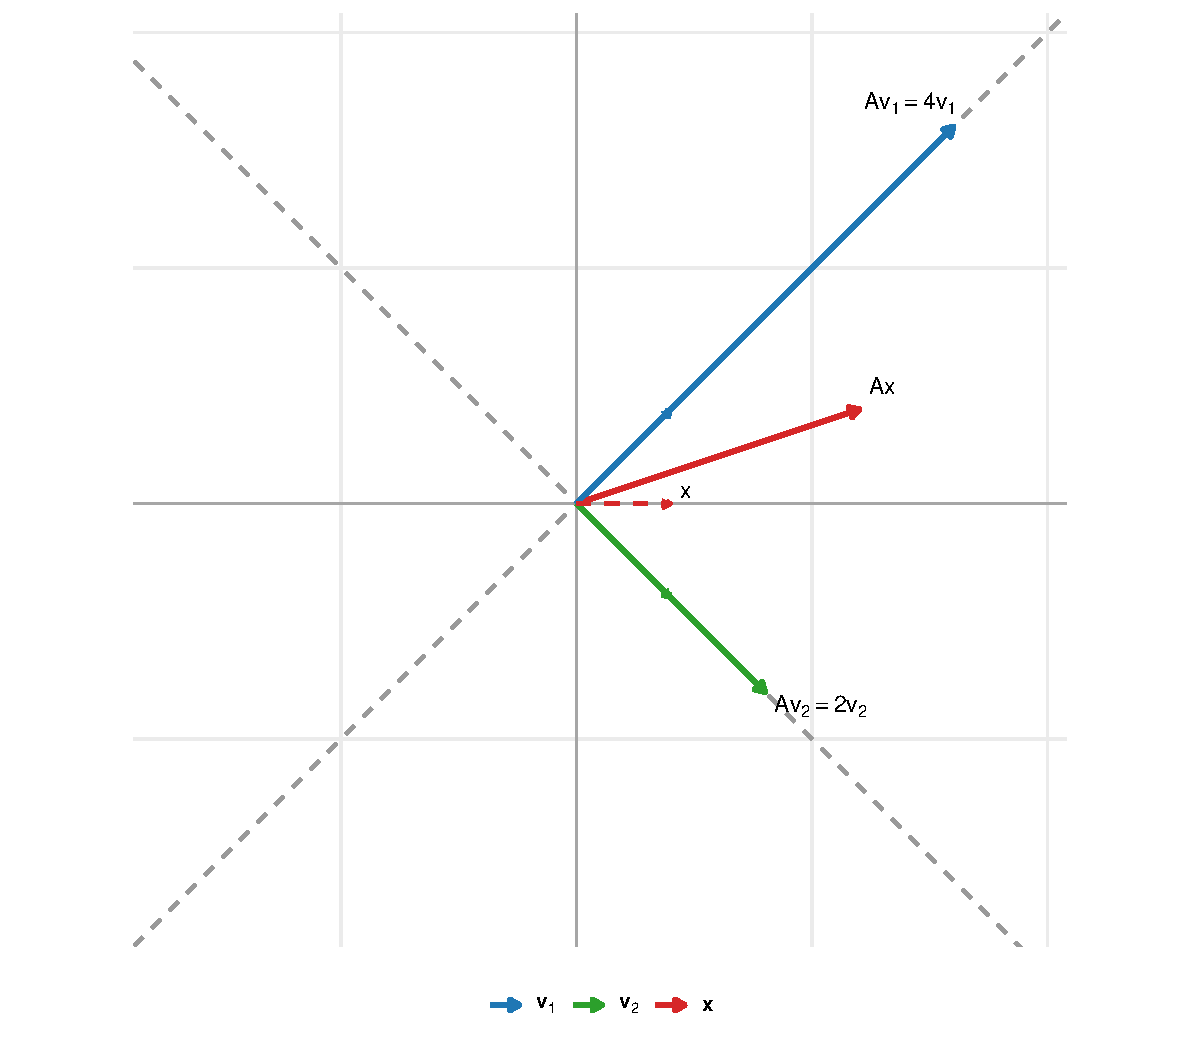
\includegraphics[keepaspectratio]{mod_1_autovetores_files/figure-pdf/fig-direcoes-invariantes-1.pdf}}

}

\caption{\label{fig-direcoes-invariantes}Autovetores permanecem nas
mesmas direções após a transformação, enquanto um vetor genérico pode
ter sua direção modificada.}

\end{figure}%

As retas tracejadas representam as direções geradas por \(\mathbf{v}_1\)
e \(\mathbf{v}_2\). A transformação amplia os vetores por fatores
diferentes, mas mantém cada um na reta correspondente. O vetor
\(\mathbf{x}\) não pertence a uma direção invariante e sua imagem ocupa
outra direção.

Um autovetor não é único. Se \(\mathbf v\) é um autovetor associado ao
autovalor \(\lambda\), então qualquer múltiplo não nulo de \(\mathbf v\)
também é um autovetor associado ao mesmo autovalor.

\begin{proposition}[Múltiplos de um
autovetor]\protect\hypertarget{prp-multiplos-autovetor}{}\label{prp-multiplos-autovetor}

Se \(\mathbf{v}\) é um autovetor de \(\mathbf{A}\) associado ao
autovalor \(\lambda\), então todo múltiplo

\[
c\mathbf{v},
\qquad
c\neq0,
\]

também é um autovetor associado a \(\lambda\).

\end{proposition}

\begin{proof}
Como

\[
\mathbf{A}\mathbf{v}
=
\lambda\mathbf{v},
\]

pela linearidade,

\[
\begin{aligned}
\mathbf{A}
\left(
c\mathbf{v}
\right)
&=
c\mathbf{A}\mathbf{v}\\
&=
c\lambda\mathbf{v}\\
&=
\lambda
\left(
c\mathbf{v}
\right).
\end{aligned}
\]

Como \(c\neq0\) e \(\mathbf{v}\neq\mathbf{0}\), tem-se
\(c\mathbf{v}\neq\mathbf{0}\). Portanto, \(c\mathbf{v}\) é um autovetor
associado a \(\lambda\).
\end{proof}

Para reunir todos os autovetores associados ao mesmo autovalor,
reorganiza-se a equação

\[
\mathbf{A}\mathbf{v}
=
\lambda\mathbf{v}
\]

como

\[
\left(
\mathbf{A}
-
\lambda\mathbf{I}_p
\right)
\mathbf{v}
=
\mathbf{0}.
\]

O conjunto de soluções é o núcleo de

\[
\mathbf{A}
-
\lambda\mathbf{I}_p.
\]

\begin{definition}[Autoespaço]\protect\hypertarget{def-autoespaco}{}\label{def-autoespaco}

Se \(\lambda\) é um autovalor de

\[
\mathbf{A}
\in
\mathbb{R}^{p\times p},
\]

o \textbf{autoespaço} associado a \(\lambda\) é

\[
\mathcal{E}_{\lambda}
=
\mathcal{N}
\left(
\mathbf{A}
-
\lambda\mathbf{I}_p
\right).
\]

Os autovetores associados a \(\lambda\) são os elementos não nulos de
\(\mathcal{E}_{\lambda}\):

\[
\mathcal{E}_{\lambda}
\setminus
\{\mathbf{0}\}.
\]

\end{definition}

O vetor nulo pertence a todo autoespaço, mas não é considerado um
autovetor. A igualdade

\[
\mathbf{A}\mathbf{0}
=
\lambda\mathbf{0}
\]

é satisfeita para qualquer \(\lambda\) e não identifica uma direção.

\begin{proposition}[Estrutura e invariância do
autoespaço]\protect\hypertarget{prp-autoespaco-invariante}{}\label{prp-autoespaco-invariante}

Se \(\lambda\) é um autovalor de \(\mathbf{A}\), então
\(\mathcal{E}_{\lambda}\) é um subespaço não trivial de \(\mathbb{R}^p\)
e é invariante sob \(\mathbf{A}\).

\end{proposition}

\begin{proof}
Como

\[
\mathcal{E}_{\lambda}
=
\mathcal{N}
\left(
\mathbf{A}
-
\lambda\mathbf{I}_p
\right),
\]

o autoespaço é o núcleo de uma transformação linear e, portanto, é um
subespaço de \(\mathbb{R}^p\).

Como \(\lambda\) é um autovalor, existe pelo menos um vetor não nulo
\(\mathbf{v}\) tal que

\[
\left(
\mathbf{A}
-
\lambda\mathbf{I}_p
\right)
\mathbf{v}
=
\mathbf{0}.
\]

Logo,

\[
\mathcal{E}_{\lambda}
\neq
\{\mathbf{0}\}.
\]

Para qualquer \(\mathbf{w}\in\mathcal{E}_{\lambda}\),

\[
\mathbf{A}\mathbf{w}
=
\lambda\mathbf{w}.
\]

Como \(\mathcal{E}_{\lambda}\) é fechado pela multiplicação por
escalares,

\[
\lambda\mathbf{w}
\in
\mathcal{E}_{\lambda}.
\]

Portanto,

\[
\mathbf{A}\mathbf{w}
\in
\mathcal{E}_{\lambda},
\]

e o autoespaço é invariante sob \(\mathbf{A}\).
\end{proof}

Quando

\[
\dim
\left(
\mathcal{E}_{\lambda}
\right)
=
1,
\]

o autoespaço determina uma única direção invariante. Todos os
autovetores associados a \(\lambda\) são múltiplos não nulos de um mesmo
vetor.

Quando

\[
\dim
\left(
\mathcal{E}_{\lambda}
\right)
>
1,
\]

o autovalor está associado a várias direções linearmente independentes.
Nesse caso, o objeto geométrico determinado pela matriz é todo o
autoespaço. Uma base específica desse subespaço não é necessariamente
única.

A definição do autoespaço transforma a busca por autovetores em um
problema de núcleo. Para um valor fixado de \(\lambda\), existem
autovetores associados precisamente quando

\[
\mathcal{N}
\left(
\mathbf{A}
-
\lambda\mathbf{I}_p
\right)
\neq
\{\mathbf{0}\}.
\]

Resta, portanto, determinar quais valores de \(\lambda\) tornam esse
núcleo não trivial. Essa condição equivale à singularidade de
\(\mathbf{A}-\lambda\mathbf{I}_p\) e conduz à equação característica.

\section{Equação característica, multiplicidades e
diagonalização}\label{equauxe7uxe3o-caracteruxedstica-multiplicidades-e-diagonalizauxe7uxe3o}

A definição de autovalor permite verificar se um vetor conhecido
determina uma direção invariante. Para encontrar essas direções a partir
de uma matriz, é necessário determinar os valores de \(\lambda\) para os
quais

\[
\left(
\mathbf{A}
-
\lambda\mathbf{I}_p
\right)
\mathbf{v}
=
\mathbf{0}
\]

possui soluções não triviais.

Esse é um sistema linear homogêneo.

Se

\[
\mathbf{A}
-
\lambda\mathbf{I}_p
\]

fosse invertível, sua única solução seria \(\mathbf{v}=\mathbf{0}\).
Portanto, um autovalor deve tornar essa matriz singular.

\begin{theorem}[Caracterização dos autovalores pelo
determinante]\protect\hypertarget{thm-caracterizacao-autovalor-determinante}{}\label{thm-caracterizacao-autovalor-determinante}

Seja

\[
\mathbf{A}
\in
\mathbb{R}^{p\times p}.
\]

Um escalar \(\lambda\in\mathbb{R}\) é autovalor de \(\mathbf{A}\) se, e
somente se,

\[
\det
\left(
\mathbf{A}
-
\lambda\mathbf{I}_p
\right)
=
0.
\]

\end{theorem}

\begin{proof}
Se \(\lambda\) é autovalor de \(\mathbf{A}\), existe um vetor não nulo
\(\mathbf{v}\) tal que

\[
\left(
\mathbf{A}
-
\lambda\mathbf{I}_p
\right)
\mathbf{v}
=
\mathbf{0}.
\]

Como o sistema possui uma solução não trivial, a matriz

\[
\mathbf{A}
-
\lambda\mathbf{I}_p
\]

não é invertível. Logo,

\[
\det
\left(
\mathbf{A}
-
\lambda\mathbf{I}_p
\right)
=
0.
\]

Reciprocamente, se

\[
\det
\left(
\mathbf{A}
-
\lambda\mathbf{I}_p
\right)
=
0,
\]

a matriz é singular. Portanto, seu núcleo contém pelo menos um vetor não
nulo \(\mathbf{v}\), para o qual

\[
\left(
\mathbf{A}
-
\lambda\mathbf{I}_p
\right)
\mathbf{v}
=
\mathbf{0}.
\]

Consequentemente,

\[
\mathbf{A}\mathbf{v}
=
\lambda\mathbf{v},
\]

e \(\lambda\) é autovalor de \(\mathbf{A}\).
\end{proof}

\begin{definition}[Polinômio e equação
característicos]\protect\hypertarget{def-polinomio-caracteristico}{}\label{def-polinomio-caracteristico}

O \textbf{polinômio característico} de uma matriz

\[
\mathbf{A}
\in
\mathbb{R}^{p\times p}
\]

é definido por

\[
p_{\mathbf{A}}(\lambda)
=
\det
\left(
\mathbf{A}
-
\lambda\mathbf{I}_p
\right).
\]

A equação

\[
p_{\mathbf{A}}(\lambda)
=
0
\]

é denominada \textbf{equação característica} de \(\mathbf{A}\). (Horn;
Johnson, 2013)

\end{definition}

Também é possível definir o polinômio característico por

\[
\det
\left(
\lambda\mathbf{I}_p
-
\mathbf{A}
\right).
\]

As duas convenções diferem pelo fator \((-1)^p\) e possuem as mesmas
raízes. Portanto, produzem os mesmos autovalores.

O polinômio característico de uma matriz de ordem \(p\) possui grau
\(p\). Consideradas suas multiplicidades, ele possui \(p\) raízes no
conjunto dos números complexos. Uma matriz real pode ter autovalores
reais, autovalores complexos ou ambos.

\subsection{Determinação dos autovalores e
autoespaços}\label{determinauxe7uxe3o-dos-autovalores-e-autoespauxe7os}

Considere novamente

\[
\mathbf{A}
=
\begin{bmatrix}
3&1\\
1&3
\end{bmatrix}.
\]

Tem-se

\[
\mathbf{A}
-
\lambda\mathbf{I}_2
=
\begin{bmatrix}
3-\lambda&1\\
1&3-\lambda
\end{bmatrix}.
\]

O polinômio característico é

\[
\begin{aligned}
p_{\mathbf{A}}(\lambda)
&=
\det
\begin{bmatrix}
3-\lambda&1\\
1&3-\lambda
\end{bmatrix}\\
&=
(3-\lambda)^2-1\\
&=
\lambda^2-6\lambda+8\\
&=
(\lambda-4)(\lambda-2).
\end{aligned}
\]

Assim, os autovalores são

\[
\lambda_1=4
\qquad
\text{e}
\qquad
\lambda_2=2.
\]

Para determinar o autoespaço associado a \(\lambda_1=4\), resolve-se

\[
\left(
\mathbf{A}
-
4\mathbf{I}_2
\right)
\mathbf{v}
=
\mathbf{0}.
\]

Como

\[
\mathbf{A}
-
4\mathbf{I}_2
=
\begin{bmatrix}
-1&1\\
1&-1
\end{bmatrix},
\]

o sistema conduz a

\[
-v_1+v_2=0,
\]

ou seja,

\[
v_2=v_1.
\]

Portanto,

\[
\mathcal{E}_4
=
\operatorname{span}
\left\{
\begin{bmatrix}
1\\
1
\end{bmatrix}
\right\}.
\]

Para \(\lambda_2=2\),

\[
\mathbf{A}
-
2\mathbf{I}_2
=
\begin{bmatrix}
1&1\\
1&1
\end{bmatrix},
\]

e o sistema correspondente fornece

\[
v_1+v_2=0.
\]

Logo,

\[
\mathcal{E}_2
=
\operatorname{span}
\left\{
\begin{bmatrix}
1\\
-1
\end{bmatrix}
\right\}.
\]

O procedimento possui duas etapas:

\begin{enumerate}
\def\labelenumi{\arabic{enumi}.}
\item
  resolver

  \[
  \det
  \left(
  \mathbf{A}
  -
  \lambda\mathbf{I}_p
  \right)
  =
  0
  \]

  para obter os autovalores;
\item
  para cada autovalor \(\lambda\), determinar

  \[
  \mathcal{E}_{\lambda}
  =
  \mathcal{N}
  \left(
  \mathbf{A}
  -
  \lambda\mathbf{I}_p
  \right).
  \]
\end{enumerate}

\subsection{Autovalores complexos de matrizes
reais}\label{autovalores-complexos-de-matrizes-reais}

As definições de autovalor, autovetor, autoespaço e equação
característica foram apresentadas inicialmente no espaço real. Elas se
estendem ao espaço complexo substituindo

\[
\mathbb{R}^p
\]

por

\[
\mathbb{C}^p
\]

e permitindo

\[
\lambda\in\mathbb{C}.
\]

Nesse caso, um autovetor complexo é um vetor não nulo
\(\mathbf{v}\in\mathbb{C}^p\) que satisfaz

\[
\mathbf{A}\mathbf{v}
=
\lambda\mathbf{v}.
\]

A caracterização

\[
\det
\left(
\mathbf{A}
-
\lambda\mathbf{I}_p
\right)
=
0
\]

permanece válida no espaço complexo.

Nem toda matriz real possui autovalores reais. Considere a rotação de
\(90^\circ\) (\(\theta= \frac{\pi}{2}\)),

\[
\mathbf{Q}_{\frac{\pi}{2}}
=
\begin{bmatrix}
\cos\left(\frac{\pi}{2}\right)
&
-\sin\left(\frac{\pi}{2}\right)
\\
\sin\left(\frac{\pi}{2}\right)
&
\cos\left(\frac{\pi}{2}\right)
\end{bmatrix}
=
\begin{bmatrix}
0&-1\\
1&0
\end{bmatrix}.
\]

Seu polinômio característico é

\[
\begin{aligned}
p_{\mathbf{Q}}(\lambda)
&=
\det
\begin{bmatrix}
-\lambda&-1\\
1&-\lambda
\end{bmatrix}\\
&=
\lambda^2+1.
\end{aligned}
\]

A equação

\[
\lambda^2+1=0
\]

não possui raízes reais. Suas raízes complexas são

\[
\lambda_1=i
\qquad
\text{e}
\qquad
\lambda_2=-i.
\]

Portanto, a matriz não possui autovalores reais e, consequentemente, não
possui autovetores reais. Geometricamente, nenhuma reta real que passa
pela origem permanece invariante sob uma rotação de \(90^\circ\).

Quando a mesma matriz é considerada como um operador em \(\mathbb C^2\),
ela possui autovalores e autovetores complexos. Neste capítulo, a
interpretação geométrica será desenvolvida principalmente no contexto
real. Em particular, toda matriz simétrica real possui autovalores reais
e admite uma base ortonormal de autovetores reais.

\subsection{Independência entre
autovetores}\label{independuxeancia-entre-autovetores}

Os autovetores associados a autovalores distintos possuem uma
propriedade que permite construir bases de direções invariantes.

\begin{theorem}[Independência de autovetores associados a autovalores
distintos]\protect\hypertarget{thm-autovetores-autovalores-distintos}{}\label{thm-autovetores-autovalores-distintos}

Se

\[
\lambda_1,\ldots,\lambda_r
\]

são autovalores distintos de uma matriz \(\mathbf{A}\) e

\[
\mathbf{v}_1,\ldots,\mathbf{v}_r
\]

são autovetores associados, respectivamente, a esses autovalores, então

\[
\mathbf{v}_1,\ldots,\mathbf{v}_r
\]

são linearmente independentes.

\end{theorem}

\begin{proof}
A demonstração será feita por indução sobre \(r\).

Para \(r=1\), o resultado é imediato porque um autovetor é não nulo.

Suponha que o resultado seja válido para \(r-1\) autovetores e considere

\[
c_1\mathbf{v}_1
+
\cdots
+
c_r\mathbf{v}_r
=
\mathbf{0}.
\]

Multiplicando por \(\mathbf{A}\),

\[
c_1\lambda_1\mathbf{v}_1
+
\cdots
+
c_r\lambda_r\mathbf{v}_r
=
\mathbf{0}.
\]

Multiplicando a primeira igualdade por \(\lambda_r\) e subtraindo-a da
segunda,

\[
c_1
\left(
\lambda_1-\lambda_r
\right)
\mathbf{v}_1
+
\cdots
+
c_{r-1}
\left(
\lambda_{r-1}-\lambda_r
\right)
\mathbf{v}_{r-1}
=
\mathbf{0}.
\]

Pela hipótese de indução,

\[
c_j
\left(
\lambda_j-\lambda_r
\right)
=
0,
\qquad
j=1,\ldots,r-1.
\]

Como os autovalores são distintos,

\[
\lambda_j-\lambda_r
\neq
0,
\]

e, portanto,

\[
c_1=\cdots=c_{r-1}=0.
\]

A igualdade original reduz-se a

\[
c_r\mathbf{v}_r
=
\mathbf{0}.
\]

Como \(\mathbf{v}_r\neq\mathbf{0}\), segue que \(c_r=0\). Logo, os
autovetores são linearmente independentes.
\end{proof}

Uma consequência imediata é que uma matriz de ordem \(p\) com \(p\)
autovalores distintos possui uma base formada por autovetores. Essa
condição é suficiente para a diagonalização, mas não é necessária: uma
matriz também pode ser diagonalizável quando possui autovalores
repetidos.

\subsection{Multiplicidades algébrica e
geométrica}\label{multiplicidades-alguxe9brica-e-geomuxe9trica}

Quando um autovalor aparece mais de uma vez como raiz do polinômio
característico, é necessário distinguir sua repetição algébrica da
dimensão do autoespaço correspondente.

\begin{definition}[Multiplicidades de um
autovalor]\protect\hypertarget{def-multiplicidades-autovalor}{}\label{def-multiplicidades-autovalor}

Seja \(\lambda\) um autovalor de \(\mathbf{A}\).

A \textbf{multiplicidade algébrica} de \(\lambda\), denotada por

\[
m_a(\lambda),
\]

é o número de vezes que \(\lambda\) aparece como raiz do polinômio
característico.

A \textbf{multiplicidade geométrica} de \(\lambda\), denotada por

\[
m_g(\lambda),
\]

é a dimensão do autoespaço correspondente:

\[
m_g(\lambda)
=
\dim
\left(
\mathcal{E}_{\lambda}
\right)
=
\dim
\mathcal{N}
\left(
\mathbf{A}
-
\lambda\mathbf{I}_p
\right).
\]

\end{definition}

Para todo autovalor,

\[
1
\leq
m_g(\lambda)
\leq
m_a(\lambda).
\]

A multiplicidade geométrica é pelo menos 1 porque o autoespaço contém
vetores não nulos. Ela representa o número máximo de autovetores
linearmente independentes que podem ser escolhidos para aquele
autovalor.

\begin{example}[Mesma multiplicidade algébrica e diferentes
multiplicidades
geométricas]\protect\hypertarget{exm-multiplicidades-algebrica-geometrica}{}\label{exm-multiplicidades-algebrica-geometrica}

Considere as matrizes

\[
\mathbf A_1
=
\begin{bmatrix}
2&0\\
0&2
\end{bmatrix}
\]

e

\[
\mathbf A_2
=
\begin{bmatrix}
2&1\\
0&2
\end{bmatrix}.
\]

\textbf{Polinômio característico e multiplicidade algébrica}

Para \(\mathbf A_1\),

\[
\begin{aligned}
p_{\mathbf A_1}(\lambda)
&=
\det
\left(
\mathbf A_1-\lambda\mathbf I_2
\right)\\
&=
\det
\begin{bmatrix}
2-\lambda&0\\
0&2-\lambda
\end{bmatrix}\\
&=
(2-\lambda)^2.
\end{aligned}
\]

Para \(\mathbf A_2\),

\[
\begin{aligned}
p_{\mathbf A_2}(\lambda)
&=
\det
\left(
\mathbf A_2-\lambda\mathbf I_2
\right)\\
&=
\det
\begin{bmatrix}
2-\lambda&1\\
0&2-\lambda
\end{bmatrix}\\
&=
(2-\lambda)^2.
\end{aligned}
\]

Portanto, as duas matrizes possuem o mesmo polinômio característico,

\[
p(\lambda)
=
(2-\lambda)^2,
\]

e, consequentemente, o mesmo autovalor,

\[
\lambda=2.
\]

Como o fator \((2-\lambda)\) aparece duas vezes no polinômio
característico, o autovalor \(\lambda=2\) possui multiplicidade
algébrica

\[
m_a(2)=2
\]

para ambas as matrizes.

\textbf{Autoespaço de \(\mathbf A_1\)}

Para determinar o autoespaço associado a \(\lambda=2\), procuramos todos
os vetores

\[
\mathbf v
=
\begin{bmatrix}
v_1\\
v_2
\end{bmatrix}
\]

que satisfazem

\[
\mathbf A_1\mathbf v
=
2\mathbf v.
\]

Essa equação pode ser escrita como

\[
\left(
\mathbf A_1-2\mathbf I_2
\right)\mathbf v
=
\mathbf0.
\]

Calculando a matriz,

\[
\begin{aligned}
\mathbf A_1-2\mathbf I_2
&=
\begin{bmatrix}
2&0\\
0&2
\end{bmatrix}
-
\begin{bmatrix}
2&0\\
0&2
\end{bmatrix}\\
&=
\begin{bmatrix}
0&0\\
0&0
\end{bmatrix}.
\end{aligned}
\]

Assim, o sistema a ser resolvido é

\[
\begin{bmatrix}
0&0\\
0&0
\end{bmatrix}
\begin{bmatrix}
v_1\\
v_2
\end{bmatrix}
=
\begin{bmatrix}
0\\
0
\end{bmatrix},
\]

ou seja,

\[
\begin{cases}
0=0,\\
0=0.
\end{cases}
\]

O sistema não impõe nenhuma restrição sobre \(v_1\) e \(v_2\). Portanto,
ambos são livres e qualquer vetor de \(\mathbb R^2\) pertence ao espaço
nulo de \(\mathbf A_1-2\mathbf I_2\).

Logo,

\[
E_2
=
\mathcal N
\left(
\mathbf A_1-2\mathbf I_2
\right)
=
\mathbb R^2.
\]

Como

\[
\dim(\mathbb R^2)=2,
\]

temos

\[
m_g(2)
=
\dim(E_2)
=
2.
\]

Assim, todo vetor não nulo de \(\mathbb R^2\) é um autovetor de
\(\mathbf A_1\) associado ao autovalor \(\lambda=2\).

\textbf{Autoespaço de \(\mathbf A_2\)}

Para \(\mathbf A_2\), procuramos novamente os vetores

\[
\mathbf v
=
\begin{bmatrix}
v_1\\
v_2
\end{bmatrix}
\]

que satisfazem

\[
\left(
\mathbf A_2-2\mathbf I_2
\right)\mathbf v
=
\mathbf0.
\]

Calculando,

\[
\begin{aligned}
\mathbf A_2-2\mathbf I_2
&=
\begin{bmatrix}
2&1\\
0&2
\end{bmatrix}
-
\begin{bmatrix}
2&0\\
0&2
\end{bmatrix}\\
&=
\begin{bmatrix}
0&1\\
0&0
\end{bmatrix}.
\end{aligned}
\]

Portanto,

\[
\begin{bmatrix}
0&1\\
0&0
\end{bmatrix}
\begin{bmatrix}
v_1\\
v_2
\end{bmatrix}
=
\begin{bmatrix}
0\\
0
\end{bmatrix}.
\]

Efetuando a multiplicação,

\[
\begin{bmatrix}
v_2\\
0
\end{bmatrix}
=
\begin{bmatrix}
0\\
0
\end{bmatrix},
\]

o que corresponde ao sistema

\[
\begin{cases}
v_2=0,\\
0=0.
\end{cases}
\]

Nesse caso, \(v_2\) deve ser igual a zero, enquanto \(v_1\) permanece
livre. Assim, todo vetor do autoespaço possui a forma

\[
\mathbf v
=
\begin{bmatrix}
v_1\\
0
\end{bmatrix}
=
v_1
\begin{bmatrix}
1\\
0
\end{bmatrix}.
\]

Logo,

\[
E_2
=
\mathcal N
\left(
\mathbf A_2-2\mathbf I_2
\right)
=
\operatorname{span}
\left\{
\begin{bmatrix}
1\\
0
\end{bmatrix}
\right\}.
\]

Esse autoespaço possui uma única direção linearmente independente.
Portanto,

\[
m_g(2)
=
\dim(E_2)
=
1.
\]

As duas matrizes possuem, portanto, o mesmo autovalor \(\lambda=2\) e a
mesma multiplicidade algébrica,

\[
m_a(2)=2,
\]

mas apresentam multiplicidades geométricas diferentes:

\[
m_g(2)
=
\begin{cases}
2, & \text{para }\mathbf A_1,\\
1, & \text{para }\mathbf A_2.
\end{cases}
\]

A diferença decorre da dimensão dos respectivos autoespaços. Para
\(\mathbf A_1\), o autoespaço é todo o plano \(\mathbb R^2\); para
\(\mathbf A_2\), o autoespaço é apenas a reta gerada por \((1,0)^\top\).

\end{example}

A Figura~\ref{fig-multiplicidades} compara as estruturas dos dois
autoespaços.

\begin{figure}

\centering{

\pandocbounded{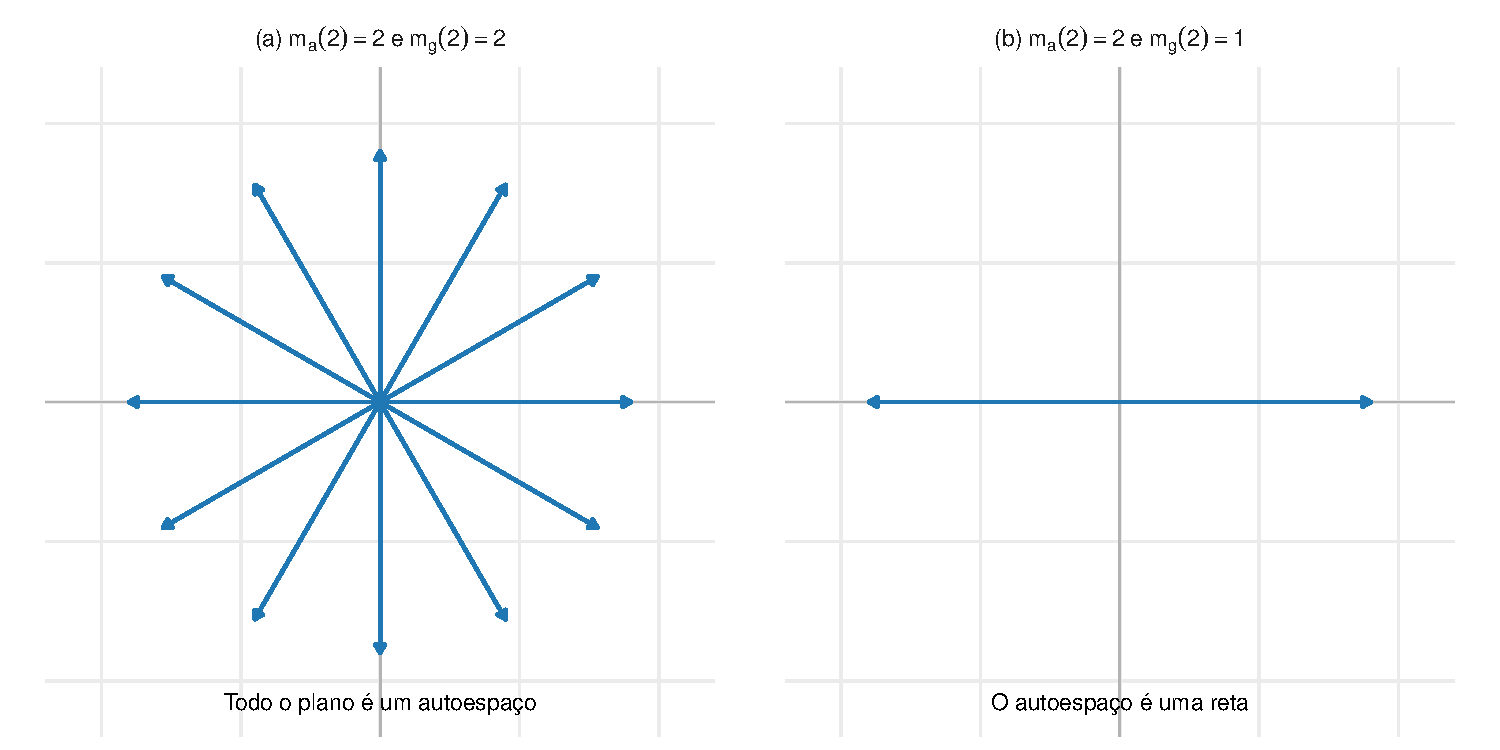
\includegraphics[keepaspectratio]{mod_1_autovetores_files/figure-pdf/fig-multiplicidades-1.pdf}}

}

\caption{\label{fig-multiplicidades}Matrizes com o mesmo autovalor
repetido podem possuir autoespaços de dimensões diferentes.}

\end{figure}%

As duas matrizes possuem o mesmo autovalor com a mesma multiplicidade
algébrica. A diferença entre as multiplicidades geométricas determina se
existem autovetores suficientes para formar uma base.

\subsection{Diagonalização}\label{diagonalizauxe7uxe3o}

No capítulo anterior, vimos que a matriz de um operador depende da base
utilizada para representá-lo. A diagonalização corresponde à escolha de
uma base particularmente conveniente: uma base formada por autovetores.

Considere uma matriz

\[\mathbf{A}\in\mathbb{R}^{p\times p}\]

e suponha que exista uma base de \(\mathbb{R}^p\) formada por
autovetores de \(\mathbf{A}\),

\[
\mathcal{B}_{\mathbf{A}}
=
\{
\mathbf{v}_1,\ldots,\mathbf{v}_p
\}.
\]

A matriz dessa base é

\[
\mathbf{B}_{\mathbf{A}}
=
\begin{bmatrix}
\mathbf{v}_1&
\cdots&
\mathbf{v}_p
\end{bmatrix}.
\]

Como os vetores da base são linearmente independentes,
\(\mathbf{B}_{\mathbf{A}}\) é invertível.

Se

\[
\mathbf{A}\mathbf{v}_j
=
\lambda_j\mathbf{v}_j,
\qquad
j=1,\ldots,p,
\]

e

\[
\boldsymbol{\Lambda}_{\mathbf{A}}
=
\operatorname{diag}
\left(
\lambda_1,\ldots,\lambda_p
\right),
\]

então

\[
\mathbf{A}\mathbf{B}_{\mathbf{A}}
=
\mathbf{B}_{\mathbf{A}}
\boldsymbol{\Lambda}_{\mathbf{A}}.
\]

Multiplicando à esquerda por \(\mathbf{B}_{\mathbf{A}}^{-1}\),

\[
\mathbf{B}_{\mathbf{A}}^{-1}
\mathbf{A}
\mathbf{B}_{\mathbf{A}}
=
\boldsymbol{\Lambda}_{\mathbf{A}}.
\]

\begin{definition}[Matriz
diagonalizável]\protect\hypertarget{def-matriz-diagonalizavel}{}\label{def-matriz-diagonalizavel}

Uma matriz

\[\mathbf{A}\in\mathbb{R}^{p\times p}\]

é \textbf{diagonalizável sobre \(\mathbb{R}\)} quando existe uma base
\(\mathcal{B}_{\mathbf{A}}\) de \(\mathbb{R}^p\) formada por autovetores
de \(\mathbf{A}\).

Equivalentemente, existem uma matriz invertível
\(\mathbf{B}_{\mathbf{A}}\) e uma matriz diagonal
\(\boldsymbol{\Lambda}_{\mathbf{A}}\) tais que

\[
\mathbf{A}
=
\mathbf{B}_{\mathbf{A}}
\boldsymbol{\Lambda}_{\mathbf{A}}
\mathbf{B}_{\mathbf{A}}^{-1}.
\]

\end{definition}

A ordem das colunas de \(\mathbf{B}_{\mathbf{A}}\) deve coincidir com a
ordem dos autovalores em \(\boldsymbol{\Lambda}_{\mathbf{A}}\).

Pela notação de mudança de base desenvolvida no capítulo anterior,

\[
[T_{\mathbf{A}}]_{\mathcal{B}_{\mathbf{A}}\leftarrow\mathcal{B}_{\mathbf{A}}}
=
\mathbf{B}_{\mathbf{A}}^{-1}
\mathbf{A}
\mathbf{B}_{\mathbf{A}}
=
\boldsymbol{\Lambda}_{\mathbf{A}}.
\]

Assim, \(\boldsymbol{\Lambda}_{\mathbf{A}}\) é a matriz do mesmo
operador quando tanto o domínio quanto o contradomínio são representados
na base de autovetores.

Para qualquer vetor \(\mathbf{x}\in\mathbb{R}^p\), suas coordenadas
nessa base são

\[
\mathbf{z}
=
[\mathbf{x}]_{\mathcal{B}_{\mathbf{A}}}
=
\mathbf{B}_{\mathbf{A}}^{-1}\mathbf{x},
\]

de modo que

\[
\mathbf{x}
=
\mathbf{B}_{\mathbf{A}}\mathbf{z}.
\]

Nas coordenadas da base de autovetores,

\[
[T_{\mathbf{A}}(\mathbf{x})]_{\mathcal{B}_{\mathbf{A}}}
=
\boldsymbol{\Lambda}_{\mathbf{A}}
[\mathbf{x}]_{\mathcal{B}_{\mathbf{A}}}.
\]

Como

\[
\boldsymbol{\Lambda}_{\mathbf{A}}
\mathbf{z}
=
\begin{bmatrix}
\lambda_1z_1\\
\vdots\\
\lambda_pz_p
\end{bmatrix},
\]

a transformação atua separadamente sobre cada coordenada: a componente
correspondente ao autovetor \(\mathbf{v}_j\) é multiplicada por
\(\lambda_j\).

A diagonalização é, portanto, uma mudança para um sistema de coordenadas
no qual as direções da base são invariantes e a ação do operador deixa
de misturar coordenadas.

\begin{theorem}[Critérios de
diagonalização]\protect\hypertarget{thm-criterios-diagonalizacao}{}\label{thm-criterios-diagonalizacao}

Seja

\[
\mathbf{A}
\in
\mathbb{F}^{p\times p},
\]

em que \(\mathbb{F}\) representa \(\mathbb{R}\) ou \(\mathbb{C}\), e
suponha que seu polinômio característico se decomponha em fatores
lineares sobre \(\mathbb{F}\).

São equivalentes:

\begin{enumerate}
\def\labelenumi{\arabic{enumi}.}
\item
  \(\mathbf{A}\) é diagonalizável sobre \(\mathbb{F}\);
\item
  \(\mathbf{A}\) possui \(p\) autovetores linearmente independentes em
  \(\mathbb{F}^p\);
\item
  existe uma base de \(\mathbb{F}^p\) formada por autovetores de
  \(\mathbf{A}\);
\item
  a soma das dimensões dos autoespaços é igual a \(p\);
\item
  para cada autovalor \(\lambda\),

  \[
  m_g(\lambda)
  =
  m_a(\lambda).
  \]
\end{enumerate}

(Horn; Johnson, 2013)

\end{theorem}

O requisito de decomposição do polinômio característico é necessário
porque uma matriz real pode não possuir todos os seus autovalores em
\(\mathbb{R}\). A matriz de rotação \(\mathbf{Q}(\pi/2)\) não é
diagonalizável sobre \(\mathbb{R}\), mas é diagonalizável sobre
\(\mathbb{C}\), pois possui dois autovalores complexos distintos.

Uma condição suficiente para a diagonalização é a existência de \(p\)
autovalores distintos. Nesse caso, o
Teorema~\ref{thm-autovetores-autovalores-distintos} garante \(p\)
autovetores linearmente independentes.

Autovalores repetidos não impedem a diagonalização. Para

\[
\mathbf{A}_1
=
2\mathbf{I}_2,
\]

tem-se

\[
m_g(2)
=
m_a(2)
=
2,
\]

e a matriz é diagonalizável.

Para

\[
\mathbf{A}_2
=
\begin{bmatrix}
2&1\\
0&2
\end{bmatrix},
\]

tem-se

\[
m_g(2)=1
<
m_a(2)=2.
\]

A matriz não possui autovetores linearmente independentes em número
suficiente para formar uma base e, portanto, não é diagonalizável.

\subsection{Potências de uma matriz
diagonalizável}\label{potuxeancias-de-uma-matriz-diagonalizuxe1vel}

A representação diagonal também simplifica o cálculo de potências. Se

\[
\mathbf{A}
=
\mathbf{B}_{\mathbf{A}}
\boldsymbol{\Lambda}_{\mathbf{A}}
\mathbf{B}_{\mathbf{A}}^{-1},
\]

então

\[
\begin{aligned}
\mathbf{A}^2
&=
\mathbf{B}_{\mathbf{A}}
\boldsymbol{\Lambda}_{\mathbf{A}}
\mathbf{B}_{\mathbf{A}}^{-1}
\mathbf{B}_{\mathbf{A}}
\boldsymbol{\Lambda}_{\mathbf{A}}
\mathbf{B}_{\mathbf{A}}^{-1}\\
&=
\mathbf{B}_{\mathbf{A}}
\boldsymbol{\Lambda}_{\mathbf{A}}^2
\mathbf{B}_{\mathbf{A}}^{-1}.
\end{aligned}
\]

De forma geral, para todo inteiro \(k\geq0\),

\[
\mathbf{A}^k
=
\mathbf{B}_{\mathbf{A}}
\boldsymbol{\Lambda}_{\mathbf{A}}^k
\mathbf{B}_{\mathbf{A}}^{-1}.
\]

Como \(\boldsymbol{\Lambda}_{\mathbf{A}}\) é diagonal,

\[
\boldsymbol{\Lambda}_{\mathbf{A}}^k
=
\operatorname{diag}
\left(
\lambda_1^k,\ldots,\lambda_p^k
\right).
\]

Assim, a aplicação repetida do operador pode ser analisada coordenada a
coordenada na base de autovetores: após \(k\) aplicações, a coordenada
associada a \(\mathbf{v}_j\) é multiplicada por \(\lambda_j^k\).

Para matrizes quadradas arbitrárias, a diagonalização pode falhar. Para
matrizes simétricas reais, existe sempre uma base ortonormal de
autovetores. Essa propriedade conduz a uma diagonalização que preserva a
geometria euclidiana.

\section{Matrizes simétricas e decomposição
espectral}\label{matrizes-simuxe9tricas-e-decomposiuxe7uxe3o-espectral}

A diagonalização estudada na seção anterior pode falhar para matrizes
quadradas arbitrárias. Uma matriz pode não possuir autovalores reais ou
pode não apresentar autovetores linearmente independentes em número
suficiente para formar uma base.

As matrizes simétricas reais possuem uma estrutura mais regular.
Retomando a Definição~\ref{def-matriz-simetrica}, uma matriz

\[
\mathbf{A}
\in
\mathbb{R}^{p\times p}
\]

é simétrica quando

\[
\mathbf{A}^{\top}
=
\mathbf{A}.
\]

Para essa classe de matrizes, todos os autovalores são reais e os
autoespaços associados a autovalores distintos são ortogonais. Como
consequência, existe uma base ortonormal de \(\mathbb{R}^p\) formada por
autovetores de \(\mathbf{A}\).

\begin{theorem}[Teorema Espectral para matrizes simétricas
reais]\protect\hypertarget{thm-teorema-espectral}{}\label{thm-teorema-espectral}

Seja

\[
\mathbf{A}
\in
\mathbb{R}^{p\times p}
\]

uma matriz simétrica. Então:

\begin{enumerate}
\def\labelenumi{\arabic{enumi}.}
\item
  todos os autovalores de \(\mathbf{A}\) são reais;
\item
  autoespaços associados a autovalores distintos são ortogonais;
\item
  existe uma base ortonormal de \(\mathbb{R}^p\) formada por autovetores
  de \(\mathbf{A}\);
\item
  existe uma matriz ortogonal

  \[
  \mathbf{Q}_{\mathbf{A}}
  \in
  \mathbb{R}^{p\times p}
  \]

  e uma matriz diagonal

  \[
  \boldsymbol{\Lambda}_{\mathbf{A}}
  \in
  \mathbb{R}^{p\times p}
  \]

  tais que

  \[
  \mathbf{A}
  =
  \mathbf{Q}_{\mathbf{A}}
  \boldsymbol{\Lambda}_{\mathbf{A}}
  \mathbf{Q}_{\mathbf{A}}^{\top}.
  \]
\end{enumerate}

(Horn; Johnson, 2013)

\end{theorem}

\begin{proof}
Para demonstrar que os autovalores são reais, considere um autovalor
possivelmente complexo \(\lambda\) e um autovetor complexo não nulo
\(\mathbf{z}\), de modo que

\[
\mathbf{A}\mathbf{z}
=
\lambda\mathbf{z}.
\]

Como \(\mathbf{A}\) é real e simétrica, ela também é hermitiana:

\[
\mathbf{A}^{*}
=
\mathbf{A},
\]

em que \(*\) representa a transposta conjugada.

Multiplicando a equação de autovalor à esquerda por \(\mathbf{z}^{*}\),

\[
\mathbf{z}^{*}\mathbf{A}\mathbf{z}
=
\lambda
\mathbf{z}^{*}\mathbf{z}.
\]

A quantidade

\[
\mathbf{z}^{*}\mathbf{A}\mathbf{z}
\]

é real, pois

\[
\left(
\mathbf{z}^{*}\mathbf{A}\mathbf{z}
\right)^{*}
=
\mathbf{z}^{*}\mathbf{A}^{*}\mathbf{z}
=
\mathbf{z}^{*}\mathbf{A}\mathbf{z}.
\]

Além disso,

\[
\mathbf{z}^{*}\mathbf{z}
>
0.
\]

Portanto,

\[
\lambda
=
\frac{
\mathbf{z}^{*}\mathbf{A}\mathbf{z}
}{
\mathbf{z}^{*}\mathbf{z}
}
\]

é real.

Considere agora dois autovetores reais \(\mathbf{v}_i\) e
\(\mathbf{v}_j\), associados a autovalores distintos \(\lambda_i\) e
\(\lambda_j\). Como

\[
\mathbf{A}\mathbf{v}_i
=
\lambda_i\mathbf{v}_i
\]

e

\[
\mathbf{A}\mathbf{v}_j
=
\lambda_j\mathbf{v}_j,
\]

tem-se

\[
\begin{aligned}
\lambda_i
\mathbf{v}_i^{\top}\mathbf{v}_j
&=
\left(
\mathbf{A}\mathbf{v}_i
\right)^{\top}
\mathbf{v}_j\\
&=
\mathbf{v}_i^{\top}
\mathbf{A}^{\top}
\mathbf{v}_j\\
&=
\mathbf{v}_i^{\top}
\mathbf{A}
\mathbf{v}_j\\
&=
\lambda_j
\mathbf{v}_i^{\top}\mathbf{v}_j.
\end{aligned}
\]

Logo,

\[
\left(
\lambda_i-\lambda_j
\right)
\mathbf{v}_i^{\top}\mathbf{v}_j
=
0.
\]

Como \(\lambda_i\neq\lambda_j\),

\[
\mathbf{v}_i^{\top}\mathbf{v}_j
=
0.
\]

Portanto, os autoespaços associados a autovalores distintos são
ortogonais.

A existência de uma base ortonormal de autovetores pode ser demonstrada
por indução sobre a ordem \(p\) da matriz. Para \(p=1\), o resultado é
imediato.

Suponha agora \(p>1\). Pelo Teorema Fundamental da Álgebra, o polinômio
característico de \(\mathbf{A}\) possui pelo menos uma raiz em
\(\mathbb{C}\). Pela primeira parte da demonstração, essa raiz é real.
Denote-a por \(\lambda_1\).

Como

\[
\det
\left(
\mathbf{A}
-
\lambda_1\mathbf{I}_p
\right)
=
0,
\]

a matriz real

\[
\mathbf{A}
-
\lambda_1\mathbf{I}_p
\]

é singular e possui um vetor não nulo real em seu núcleo. Normalizando
esse vetor, obtém-se um autovetor unitário \(\mathbf{q}_1\).

Considere o complemento ortogonal

\[
\mathcal{W}
=
\operatorname{span}
\left\{
\mathbf{q}_1
\right\}^{\perp}.
\]

Para qualquer \(\mathbf{x}\in\mathcal{W}\),

\[
\mathbf{q}_1^{\top}\mathbf{x}
=
0.
\]

Como \(\mathbf{A}\) é simétrica,

\[
\begin{aligned}
\mathbf{q}_1^{\top}
\mathbf{A}\mathbf{x}
&=
\left(
\mathbf{A}\mathbf{q}_1
\right)^{\top}
\mathbf{x}\\
&=
\lambda_1
\mathbf{q}_1^{\top}\mathbf{x}\\
&=
0.
\end{aligned}
\]

Logo,

\[
\mathbf{A}\mathbf{x}
\in
\mathcal{W},
\]

e \(\mathcal{W}\) é invariante sob \(\mathbf{A}\).

A restrição de \(\mathbf{A}\) a \(\mathcal{W}\) permanece simétrica.
Como

\[
\dim(\mathcal{W})
=
p-1,
\]

a hipótese de indução garante uma base ortonormal

\[
\mathbf{q}_2,\ldots,\mathbf{q}_p
\]

de \(\mathcal{W}\) formada por autovetores da restrição e,
consequentemente, de \(\mathbf{A}\).

Assim,

\[
\mathbf{q}_1,\ldots,\mathbf{q}_p
\]

formam uma base ortonormal de \(\mathbb{R}^p\) composta por autovetores
de \(\mathbf{A}\).

Organizando esses vetores nas colunas de

\[
\mathbf{Q}_{\mathbf{A}}
=
\begin{bmatrix}
\mathbf{q}_1&
\cdots&
\mathbf{q}_p
\end{bmatrix},
\]

tem-se

\[
\mathbf{Q}_{\mathbf{A}}^{\top}
\mathbf{Q}_{\mathbf{A}}
=
\mathbf{I}_p.
\]

Portanto,

\[
\mathbf{Q}_{\mathbf{A}}^{-1}
=
\mathbf{Q}_{\mathbf{A}}^{\top}.
\]

Definindo

\[
\boldsymbol{\Lambda}_{\mathbf{A}}
=
\operatorname{diag}
\left(
\lambda_1,\ldots,\lambda_p
\right),
\]

a relação

\[
\mathbf{A}
\mathbf{Q}_{\mathbf{A}}
=
\mathbf{Q}_{\mathbf{A}}
\boldsymbol{\Lambda}_{\mathbf{A}}
\]

fornece

\[
\mathbf{A}
=
\mathbf{Q}_{\mathbf{A}}
\boldsymbol{\Lambda}_{\mathbf{A}}
\mathbf{Q}_{\mathbf{A}}^{\top}.
\]
\end{proof}

A representação

\[
\mathbf{A}
=
\mathbf{Q}_{\mathbf{A}}
\boldsymbol{\Lambda}_{\mathbf{A}}
\mathbf{Q}_{\mathbf{A}}^{\top}
\]

é denominada \textbf{decomposição espectral} de \(\mathbf{A}\). Ela é
uma diagonalização ortogonal.

Considere a base ortonormal de autovetores

\[
\mathcal{B}_{\mathbf{A}}
=
\{
\mathbf{q}_1,\ldots,\mathbf{q}_p
\}.
\]

A matriz dessa base é

\[
\mathbf{Q}_{\mathbf{A}}
=
\begin{bmatrix}
\mathbf{q}_1&
\cdots&
\mathbf{q}_p
\end{bmatrix}.
\]

Assim, no caso simétrico, a matriz da base de autovetores introduzida na
seção anterior pode ser escolhida ortogonal:

\[
\mathbf{B}_{\mathbf{A}}
=
\mathbf{Q}_{\mathbf{A}},
\]

com

\[
\mathbf{Q}_{\mathbf{A}}^{-1}
=
\mathbf{Q}_{\mathbf{A}}^{\top}.
\]

Pela notação de coordenadas desenvolvida no capítulo anterior,

\[
[\mathbf{x}]_{\mathcal{B}_{\mathbf{A}}}
=
\mathbf{Q}_{\mathbf{A}}^{\top}
\mathbf{x}.
\]

Denotando

\[
\mathbf{z}
=
[\mathbf{x}]_{\mathcal{B}_{\mathbf{A}}},
\]

tem-se

\[
\mathbf{x}
=
\mathbf{Q}_{\mathbf{A}}
\mathbf{z}.
\]

A matriz do operador nessa base é

\[
[T_{\mathbf{A}}]_{\mathcal{B}_{\mathbf{A}}\leftarrow\mathcal{B}_{\mathbf{A}}}
=
\mathbf{Q}_{\mathbf{A}}^{\top}
\mathbf{A}
\mathbf{Q}_{\mathbf{A}}
=
\boldsymbol{\Lambda}_{\mathbf{A}}.
\]

Consequentemente,

\[
[T_{\mathbf{A}}(\mathbf{x})]_{\mathcal{B}_{\mathbf{A}}}
=
\boldsymbol{\Lambda}_{\mathbf{A}}
[\mathbf{x}]_{\mathcal{B}_{\mathbf{A}}}.
\]

Em coordenadas canônicas,

\[
\begin{aligned}
\mathbf{A}\mathbf{x}
&=
\mathbf{Q}_{\mathbf{A}}
\boldsymbol{\Lambda}_{\mathbf{A}}
\mathbf{Q}_{\mathbf{A}}^{\top}
\mathbf{x}\\
&=
\mathbf{Q}_{\mathbf{A}}
\boldsymbol{\Lambda}_{\mathbf{A}}
\mathbf{z}.
\end{aligned}
\]

A ação da matriz pode ser interpretada em três etapas:

\begin{enumerate}
\def\labelenumi{\arabic{enumi}.}
\tightlist
\item
  \(\mathbf{Q}_{\mathbf{A}}^{\top}\) converte o vetor para as
  coordenadas da base ortonormal de autovetores;
\item
  \(\boldsymbol{\Lambda}_{\mathbf{A}}\) multiplica separadamente cada
  coordenada pelo autovalor correspondente;
\item
  \(\mathbf{Q}_{\mathbf{A}}\) reconstrói o vetor nas coordenadas
  canônicas.
\end{enumerate}

Assim, uma matriz simétrica atua por fatores escalares independentes em
direções ortogonais. Quando algum autovalor é negativo, o escalonamento
na direção correspondente inclui também a inversão do sentido.

\subsection{Decomposição espectral do exemplo
condutor}\label{decomposiuxe7uxe3o-espectral-do-exemplo-condutor}

\begin{example}[Decomposição espectral de uma matriz
simétrica]\protect\hypertarget{exm-decomposicao-espectral}{}\label{exm-decomposicao-espectral}

Considere novamente

\[
\mathbf{A}
=
\begin{bmatrix}
3&1\\
1&3
\end{bmatrix}.
\]

Os autovalores são

\[
\lambda_1=4
\qquad
\text{e}
\qquad
\lambda_2=2.
\]

Os autovetores

\[
\mathbf{v}_1
=
\begin{bmatrix}
1\\
1
\end{bmatrix}
\]

e

\[
\mathbf{v}_2
=
\begin{bmatrix}
1\\
-1
\end{bmatrix}
\]

são ortogonais, pois

\[
\mathbf{v}_1^{\top}\mathbf{v}_2
=
0.
\]

Normalizando-os, obtêm-se

\[
\mathbf{q}_1
=
\frac{1}{\sqrt{2}}
\begin{bmatrix}
1\\
1
\end{bmatrix}
\]

e

\[
\mathbf{q}_2
=
\frac{1}{\sqrt{2}}
\begin{bmatrix}
1\\
-1
\end{bmatrix}.
\]

Portanto,

\[
\mathcal{B}_{\mathbf{A}}
=
\{
\mathbf{q}_1,\mathbf{q}_2
\}
\]

é uma base ortonormal de autovetores de \(\mathbb{R}^2\).

A matriz dessa base é a matriz ortogonal

\[
\mathbf{Q}_{\mathbf{A}}
=
\frac{1}{\sqrt{2}}
\begin{bmatrix}
1&1\\
1&-1
\end{bmatrix},
\]

e a matriz diagonal de autovalores é

\[
\boldsymbol{\Lambda}_{\mathbf{A}}
=
\begin{bmatrix}
4&0\\
0&2
\end{bmatrix}.
\]

Consequentemente,

\[
\mathbf{A}
=
\mathbf{Q}_{\mathbf{A}}
\boldsymbol{\Lambda}_{\mathbf{A}}
\mathbf{Q}_{\mathbf{A}}^{\top}.
\]

De fato,

\[
\begin{aligned}
\mathbf{Q}_{\mathbf{A}}
\boldsymbol{\Lambda}_{\mathbf{A}}
\mathbf{Q}_{\mathbf{A}}^{\top}
&=
\frac{1}{\sqrt{2}}
\begin{bmatrix}
1&1\\
1&-1
\end{bmatrix}
\begin{bmatrix}
4&0\\
0&2
\end{bmatrix}
\frac{1}{\sqrt{2}}
\begin{bmatrix}
1&1\\
1&-1
\end{bmatrix}\\
&=
\begin{bmatrix}
3&1\\
1&3
\end{bmatrix}.
\end{aligned}
\]

Na direção de \(\mathbf{q}_1\), a transformação multiplica o comprimento
por 4. Na direção ortogonal \(\mathbf{q}_2\), multiplica o comprimento
por 2.

\end{example}

A Figura~\ref{fig-interpretacao-espectral} mostra a circunferência
unitária em \(\mathbb{R}^2\) e sua imagem pela matriz \(\mathbf{A}\).
Como os dois autovalores são positivos, a imagem é uma elipse cujos
semieixos possuem comprimentos 4 e 2 e estão alinhados aos autovetores.

\begin{figure}

\centering{

\pandocbounded{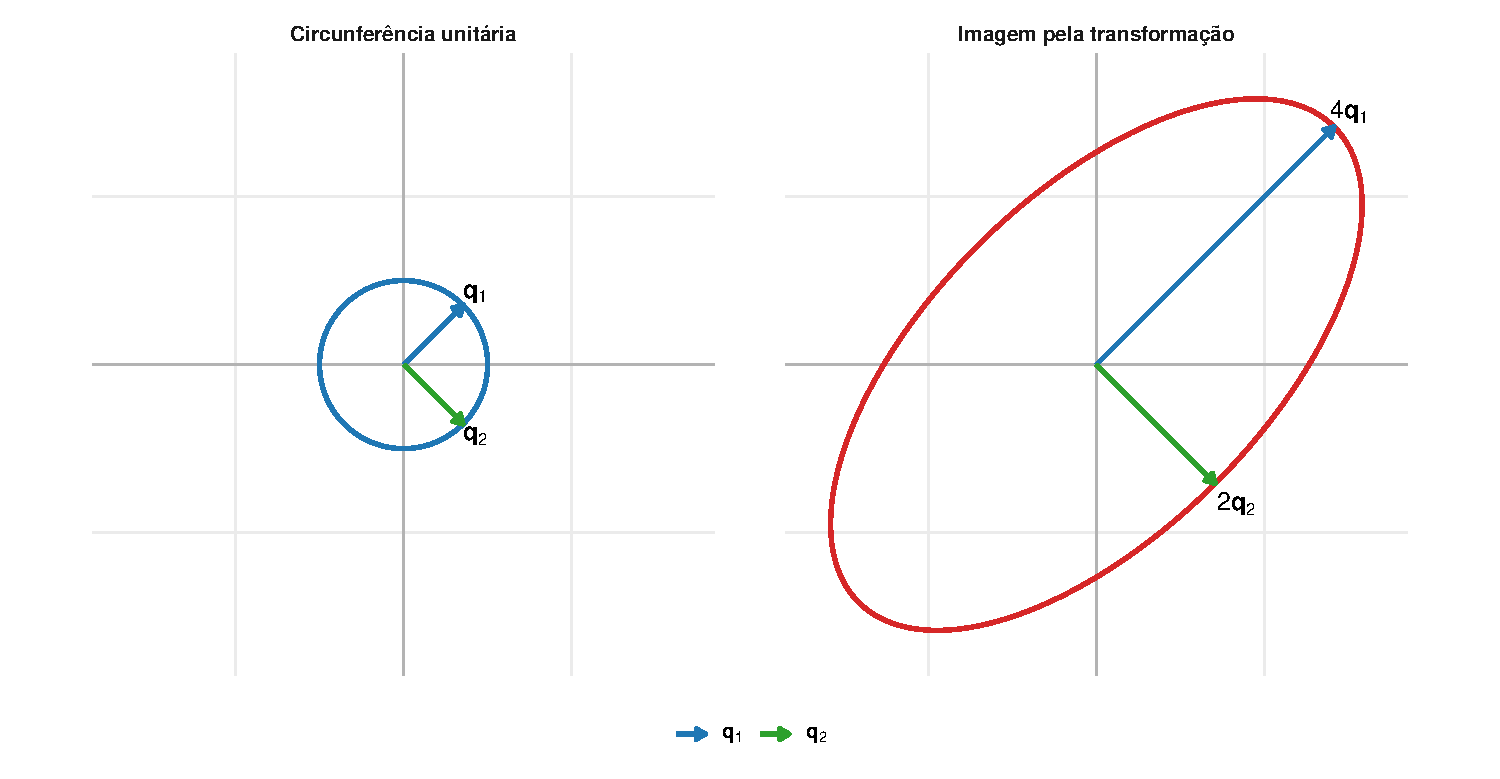
\includegraphics[keepaspectratio]{mod_1_autovetores_files/figure-pdf/fig-interpretacao-espectral-1.pdf}}

}

\caption{\label{fig-interpretacao-espectral}A decomposição espectral
identifica as direções ortogonais nas quais uma matriz simétrica atua
por fatores escalares independentes.}

\end{figure}%

Na base canônica, a ação da matriz combina as duas coordenadas. Na base
formada por \(\mathbf{q}_1\) e \(\mathbf{q}_2\), a transformação apenas
multiplica as coordenadas por 4 e 2.

Para uma matriz simétrica arbitrária, os comprimentos dos semieixos da
imagem da esfera unitária em \(\mathbb{R}^p\) são determinados por

\[
|\lambda_1|,
\ldots,
|\lambda_p|.
\]

Autovalores negativos também invertem o sentido ao longo das direções
correspondentes. Autovalores nulos colapsam os respectivos eixos,
reduzindo a dimensão da imagem.

\subsection{Forma aditiva da decomposição
espectral}\label{forma-aditiva-da-decomposiuxe7uxe3o-espectral}

Como

\[
\mathbf{Q}_{\mathbf{A}}
=
\begin{bmatrix}
\mathbf{q}_1&
\cdots&
\mathbf{q}_p
\end{bmatrix}
\]

e

\[
\boldsymbol{\Lambda}_{\mathbf{A}}
=
\operatorname{diag}
\left(
\lambda_1,\ldots,\lambda_p
\right),
\]

a decomposição espectral também pode ser escrita como

\[
\mathbf{A}
=
\sum_{j=1}^{p}
\lambda_j
\mathbf{q}_j
\mathbf{q}_j^{\top}.
\]

Cada matriz

\[
\mathbf{q}_j
\mathbf{q}_j^{\top}
\]

é o projetor ortogonal sobre a reta gerada por \(\mathbf{q}_j\). Assim,

\[
\mathbf{A}\mathbf{x}
=
\sum_{j=1}^{p}
\lambda_j
\mathbf{q}_j
\mathbf{q}_j^{\top}
\mathbf{x}.
\]

A transformação pode ser interpretada como:

\begin{enumerate}
\def\labelenumi{\arabic{enumi}.}
\tightlist
\item
  projetar \(\mathbf{x}\) sobre cada direção espectral;
\item
  multiplicar cada projeção pelo autovalor correspondente;
\item
  somar as parcelas resultantes.
\end{enumerate}

No exemplo,

\[
\mathbf{A}
=
4
\mathbf{q}_1
\mathbf{q}_1^{\top}
+
2
\mathbf{q}_2
\mathbf{q}_2^{\top}.
\]

\subsection{Projetores sobre
autoespaços}\label{projetores-sobre-autoespauxe7os}

Quando um autovalor possui multiplicidade maior que 1, os autovetores
individuais associados a ele não são únicos. O autoespaço, entretanto, é
determinado pela matriz.

Considere os autovalores distintos

\[
\lambda^{(1)},
\ldots,
\lambda^{(s)}
\]

de \(\mathbf{A}\). Para cada autovalor \(\lambda^{(h)}\), seja

\[
\mathbf{Q}_h
\]

uma matriz cujas colunas formam uma base ortonormal do autoespaço
correspondente.

Define-se o projetor espectral

\[
\boldsymbol{\Pi}_{\lambda^{(h)}}
=
\mathbf{Q}_h
\mathbf{Q}_h^{\top}.
\]

Esse projetor não depende da base ortonormal escolhida dentro do
autoespaço.

\begin{proposition}[Decomposição por projetores
espectrais]\protect\hypertarget{prp-decomposicao-projetores-espectrais}{}\label{prp-decomposicao-projetores-espectrais}

Se \(\mathbf{A}\) é simétrica e possui autovalores distintos

\[
\lambda^{(1)},
\ldots,
\lambda^{(s)},
\]

então

\[
\mathbf{A}
=
\sum_{h=1}^{s}
\lambda^{(h)}
\boldsymbol{\Pi}_{\lambda^{(h)}}.
\]

Além disso,

\[
\boldsymbol{\Pi}_{\lambda^{(h)}}^{\top}
=
\boldsymbol{\Pi}_{\lambda^{(h)}},
\]

\[
\boldsymbol{\Pi}_{\lambda^{(h)}}^2
=
\boldsymbol{\Pi}_{\lambda^{(h)}},
\]

\[
\boldsymbol{\Pi}_{\lambda^{(h)}}
\boldsymbol{\Pi}_{\lambda^{(\ell)}}
=
\mathbf{0},
\qquad
h\neq\ell,
\]

e

\[
\sum_{h=1}^{s}
\boldsymbol{\Pi}_{\lambda^{(h)}}
=
\mathbf{I}_p.
\]

(Horn; Johnson, 2013)

\end{proposition}

\begin{proof}
As colunas de \(\mathbf{Q}_h\) são ortonormais. Portanto,

\[
\boldsymbol{\Pi}_{\lambda^{(h)}}
=
\mathbf{Q}_h
\mathbf{Q}_h^{\top}
\]

é o projetor ortogonal sobre o autoespaço associado a \(\lambda^{(h)}\).
Pela Proposição~\ref{prp-propriedades-matriz-projecao}, ele é simétrico
e idempotente.

Autoespaços associados a autovalores distintos são ortogonais. Logo,

\[
\mathbf{Q}_h^{\top}\mathbf{Q}_{\ell}
=
\mathbf{0}
\]

para \(h\neq\ell\), e

\[
\begin{aligned}
\boldsymbol{\Pi}_{\lambda^{(h)}}
\boldsymbol{\Pi}_{\lambda^{(\ell)}}
&=
\mathbf{Q}_h
\mathbf{Q}_h^{\top}
\mathbf{Q}_{\ell}
\mathbf{Q}_{\ell}^{\top}\\
&=
\mathbf{0}.
\end{aligned}
\]

A soma direta ortogonal de todos os autoespaços é \(\mathbb{R}^p\). Por
isso,

\[
\sum_{h=1}^{s}
\boldsymbol{\Pi}_{\lambda^{(h)}}
=
\mathbf{I}_p.
\]

Agrupando na decomposição espectral todos os autovetores associados ao
mesmo autovalor,

\[
\mathbf{A}
=
\sum_{h=1}^{s}
\lambda^{(h)}
\boldsymbol{\Pi}_{\lambda^{(h)}}.
\]
\end{proof}

A decomposição por projetores separa o que depende de uma escolha de
base do que é determinado pelo operador. Quando um autovalor é simples,
o projetor correspondente possui posto 1:

\[
\boldsymbol{\Pi}_{\lambda}
=
\mathbf{q}\mathbf{q}^{\top}.
\]

Quando sua multiplicidade geométrica é maior que 1, o projetor
representa todo o autoespaço e possui posto igual à sua dimensão.

\subsection{Não unicidade da matriz de
autovetores}\label{nuxe3o-unicidade-da-matriz-de-autovetores}

A matriz

\[
\mathbf{Q}_{\mathbf{A}}
\]

não é necessariamente única.

Mesmo quando todos os autovalores são distintos, cada autovetor pode ser
substituído por seu oposto:

\[
\mathbf{q}_j
\longmapsto
-\mathbf{q}_j.
\]

A ordem dos autovetores também pode ser alterada, desde que a mesma
alteração seja aplicada aos autovalores em

\[
\boldsymbol{\Lambda}_{\mathbf{A}}.
\]

Quando há autovalores repetidos, qualquer base ortonormal do autoespaço
correspondente pode ser utilizada.

Essas alterações não modificam a matriz original nem os projetores
espectrais. O sinal, a ordem e a base escolhida dentro de um autoespaço
são elementos da representação; os autovalores, os autoespaços e seus
projetores são propriedades do operador.

A decomposição espectral fornece uma base ortonormal na qual formas
quadráticas, determinantes, traços, postos, inversas e superfícies de
nível podem ser analisados diretamente a partir dos autovalores.

\section{Consequências da decomposição
espectral}\label{consequuxeancias-da-decomposiuxe7uxe3o-espectral}

Considere uma matriz simétrica

\[
\mathbf{A}
\in
\mathbb{R}^{p\times p}
\]

com decomposição espectral

\[
\mathbf{A}
=
\mathbf{Q}_{\mathbf{A}}
\boldsymbol{\Lambda}_{\mathbf{A}}
\mathbf{Q}_{\mathbf{A}}^{\top},
\]

em que

\[
\mathbf{Q}_{\mathbf{A}}
=
\begin{bmatrix}
\mathbf{q}_1&
\cdots&
\mathbf{q}_p
\end{bmatrix}
\]

é ortogonal e

\[
\boldsymbol{\Lambda}_{\mathbf{A}}
=
\operatorname{diag}
\left(
\lambda_1,\ldots,\lambda_p
\right).
\]

A representação diagonal permite obter propriedades da matriz
diretamente de seus autovalores e autoespaços.

\subsection{Traço, determinante, posto e
invertibilidade}\label{trauxe7o-determinante-posto-e-invertibilidade}

\begin{proposition}[Consequências espectrais
básicas]\protect\hypertarget{prp-consequencias-espectrais-basicas}{}\label{prp-consequencias-espectrais-basicas}

Se \(\mathbf{A}\in\mathbb{R}^{p\times p}\) é simétrica e possui
autovalores

\[
\lambda_1,\ldots,\lambda_p,
\]

contados com suas multiplicidades algébricas, então:

\[
\operatorname{tr}(\mathbf{A})
=
\sum_{j=1}^{p}\lambda_j,
\]

\[
\det(\mathbf{A})
=
\prod_{j=1}^{p}\lambda_j,
\]

\[
\operatorname{posto}(\mathbf{A})
=
\#\left\{
j:
\lambda_j\neq0
\right\},
\]

e

\[
\dim
\mathcal{N}(\mathbf{A})
=
\#\left\{
j:
\lambda_j=0
\right\}.
\]

Além disso,

\[
\mathbf{A}
\text{ é invertível}
\iff
\lambda_j\neq0
\quad
\text{para todo }j.
\]

\end{proposition}

\begin{proof}
Pela propriedade cíclica do traço,

\[
\begin{aligned}
\operatorname{tr}(\mathbf{A})
&=
\operatorname{tr}
\left(
\mathbf{Q}_{\mathbf{A}}
\boldsymbol{\Lambda}_{\mathbf{A}}
\mathbf{Q}_{\mathbf{A}}^{\top}
\right)\\
&=
\operatorname{tr}
\left(
\boldsymbol{\Lambda}_{\mathbf{A}}
\mathbf{Q}_{\mathbf{A}}^{\top}
\mathbf{Q}_{\mathbf{A}}
\right)\\
&=
\operatorname{tr}
\left(
\boldsymbol{\Lambda}_{\mathbf{A}}
\right)\\
&=
\sum_{j=1}^{p}\lambda_j.
\end{aligned}
\]

Para o determinante,

\[
\begin{aligned}
\det(\mathbf{A})
&=
\det
\left(
\mathbf{Q}_{\mathbf{A}}
\right)
\det
\left(
\boldsymbol{\Lambda}_{\mathbf{A}}
\right)
\det
\left(
\mathbf{Q}_{\mathbf{A}}^{\top}
\right)\\
&=
\det
\left(
\boldsymbol{\Lambda}_{\mathbf{A}}
\right),
\end{aligned}
\]

pois

\[
\det
\left(
\mathbf{Q}_{\mathbf{A}}
\right)
\det
\left(
\mathbf{Q}_{\mathbf{A}}^{\top}
\right)
=
\det
\left(
\mathbf{I}_p
\right)
=
1.
\]

Como \(\boldsymbol{\Lambda}_{\mathbf{A}}\) é diagonal,

\[
\det(\mathbf{A})
=
\prod_{j=1}^{p}\lambda_j.
\]

As matrizes \(\mathbf{A}\) e \(\boldsymbol{\Lambda}_{\mathbf{A}}\) são
semelhantes, pois

\[
\boldsymbol{\Lambda}_{\mathbf{A}}
=
\mathbf{Q}_{\mathbf{A}}^{\top}
\mathbf{A}
\mathbf{Q}_{\mathbf{A}}.
\]

Como a multiplicação à esquerda e à direita por matrizes invertíveis
preserva o posto, \(\mathbf{A}\) e \(\boldsymbol{\Lambda}_{\mathbf{A}}\)
possuem o mesmo posto. O posto de uma matriz diagonal é igual ao número
de elementos diagonais não nulos. Portanto,

\[
\operatorname{posto}(\mathbf{A})
=
\#\left\{
j:
\lambda_j\neq0
\right\}.
\]

Pelo Teorema Posto--Nulidade,

\[
\begin{aligned}
\dim
\mathcal{N}(\mathbf{A})
&=
p-\operatorname{posto}(\mathbf{A})\\
&=
\#\left\{
j:
\lambda_j=0
\right\}.
\end{aligned}
\]

Por fim, \(\mathbf{A}\) é invertível se, e somente se, seu determinante
é diferente de zero. Como

\[
\det(\mathbf{A})
=
\prod_{j=1}^{p}\lambda_j,
\]

isso ocorre exatamente quando todos os autovalores são não nulos.
\end{proof}

Os autoespaços também fornecem descrições diretas do núcleo e da imagem.

\begin{proposition}[Núcleo e imagem em termos dos
autovetores]\protect\hypertarget{prp-nucleo-imagem-espectral}{}\label{prp-nucleo-imagem-espectral}

Se

\[
\mathbf{A}
=
\sum_{j=1}^{p}
\lambda_j
\mathbf{q}_j
\mathbf{q}_j^{\top}
\]

é a decomposição espectral de uma matriz simétrica, então

\[
\ker(T_{\mathbf{A}})
=
\mathcal{N}(\mathbf{A})
=
\operatorname{span}
\left\{
\mathbf{q}_j:
\lambda_j=0
\right\}
\]

e

\[
\operatorname{Im}(T_{\mathbf{A}})
=
\mathcal{C}(\mathbf{A})
=
\operatorname{span}
\left\{
\mathbf{q}_j:
\lambda_j\neq0
\right\}.
\]

Consequentemente,

\[
\operatorname{Im}(T_{\mathbf{A}})
=
\ker(T_{\mathbf{A}})^{\perp},
\]

ou, equivalentemente,

\[
\mathcal{C}(\mathbf{A})
=
\mathcal{N}(\mathbf{A})^{\perp}.
\]

\end{proposition}

\begin{proof}
Todo vetor \(\mathbf{x}\in\mathbb{R}^p\) pode ser escrito na base
ortonormal de autovetores como

\[
\mathbf{x}
=
\sum_{j=1}^{p}
z_j\mathbf{q}_j,
\]

em que

\[
z_j
=
\mathbf{q}_j^{\top}\mathbf{x}.
\]

Aplicando \(\mathbf{A}\),

\[
\mathbf{A}\mathbf{x}
=
\sum_{j=1}^{p}
\lambda_jz_j\mathbf{q}_j.
\]

A igualdade

\[
\mathbf{A}\mathbf{x}
=
\mathbf{0}
\]

ocorre se, e somente se,

\[
\lambda_jz_j=0
\]

para todo \(j\). Portanto, as coordenadas de \(\mathbf{x}\) podem ser
não nulas apenas nas direções associadas a autovalores iguais a zero.
Logo,

\[
\mathcal{N}(\mathbf{A})
=
\operatorname{span}
\left\{
\mathbf{q}_j:
\lambda_j=0
\right\}.
\]

Toda imagem \(\mathbf{A}\mathbf{x}\) é uma combinação linear dos
autovetores associados a autovalores não nulos. Assim,

\[
\mathcal{C}(\mathbf{A})
\subseteq
\operatorname{span}
\left\{
\mathbf{q}_j:
\lambda_j\neq0
\right\}.
\]

Reciprocamente, se \(\lambda_j\neq0\), então

\[
\mathbf{q}_j
=
\mathbf{A}
\left(
\frac{1}{\lambda_j}
\mathbf{q}_j
\right),
\]

de modo que \(\mathbf{q}_j\in\mathcal{C}(\mathbf{A})\). Portanto,

\[
\mathcal{C}(\mathbf{A})
=
\operatorname{span}
\left\{
\mathbf{q}_j:
\lambda_j\neq0
\right\}.
\]

Como os autovetores associados a autovalores nulos são ortogonais aos
autovetores associados a autovalores não nulos, e juntos formam uma base
ortonormal de \(\mathbb{R}^p\), os dois subespaços são complementos
ortogonais.
\end{proof}

O autoespaço associado ao autovalor zero reúne exatamente as direções
eliminadas pela transformação. Os autoespaços associados a autovalores
não nulos constituem, em conjunto, a imagem da transformação.

\subsection{Formas quadráticas em coordenadas
espectrais}\label{formas-quadruxe1ticas-em-coordenadas-espectrais}

Retomando a Definição~\ref{def-forma-quadratica}, considere

\[
q_{\mathbf{A}}(\mathbf{x})
=
\mathbf{x}^{\top}
\mathbf{A}
\mathbf{x}.
\]

As coordenadas de \(\mathbf{x}\) na base espectral são

\[
\mathbf{z}
=
[\mathbf{x}]_{\mathcal{B}_{\mathbf{A}}}
=
\mathbf{Q}_{\mathbf{A}}^{\top}
\mathbf{x}.
\]

Como

\[
\mathbf{x}
=
\mathbf{Q}_{\mathbf{A}}\mathbf{z},
\]

tem-se

\[
\begin{aligned}
q_{\mathbf{A}}(\mathbf{x})
&=
\mathbf{x}^{\top}
\mathbf{A}
\mathbf{x}\\
&=
\mathbf{z}^{\top}
\mathbf{Q}_{\mathbf{A}}^{\top}
\mathbf{Q}_{\mathbf{A}}
\boldsymbol{\Lambda}_{\mathbf{A}}
\mathbf{Q}_{\mathbf{A}}^{\top}
\mathbf{Q}_{\mathbf{A}}
\mathbf{z}\\
&=
\mathbf{z}^{\top}
\boldsymbol{\Lambda}_{\mathbf{A}}
\mathbf{z}\\
&=
\sum_{j=1}^{p}
\lambda_jz_j^2.
\end{aligned}
\]

A mudança ortogonal de coordenadas elimina os produtos cruzados. A
contribuição da direção \(\mathbf{q}_j\) para a forma quadrática é

\[
\lambda_jz_j^2.
\]

As possibilidades de sinal da forma quadrática são determinadas pelos
sinais dos autovalores, enquanto o valor assumido para um vetor
específico depende também de suas coordenadas espectrais
\(z_1,\ldots,z_p\).

\begin{example}[Forma quadrática em coordenadas
espectrais]\protect\hypertarget{exm-forma-quadratica-coordenadas-espectrais}{}\label{exm-forma-quadratica-coordenadas-espectrais}

Considere a matriz simétrica

\[
\mathbf A
=
\begin{bmatrix}
2&1\\
1&2
\end{bmatrix}.
\]

Seus autovalores são

\[
\lambda_1=3
\qquad\text{e}\qquad
\lambda_2=1,
\]

com autovetores ortonormais associados

\[
\mathbf q_1
=
\frac{1}{\sqrt{2}}
\begin{bmatrix}
1\\
1
\end{bmatrix},
\qquad
\mathbf q_2
=
\frac{1}{\sqrt{2}}
\begin{bmatrix}
1\\
-1
\end{bmatrix}.
\]

Portanto,

\[
\mathbf Q_{\mathbf A}
=
\frac{1}{\sqrt{2}}
\begin{bmatrix}
1&1\\
1&-1
\end{bmatrix}
\]

e

\[
\boldsymbol{\Lambda}_{\mathbf A}
=
\begin{bmatrix}
3&0\\
0&1
\end{bmatrix}.
\]

A decomposição espectral de \(\mathbf A\) é

\[
\mathbf A
=
\mathbf Q_{\mathbf A}
\boldsymbol{\Lambda}_{\mathbf A}
\mathbf Q_{\mathbf A}^{\top}.
\]

Considere agora o vetor

\[
\mathbf x
=
\begin{bmatrix}
2\\
1
\end{bmatrix}.
\]

Nas coordenadas originais, a forma quadrática é

\[
\begin{aligned}
q_{\mathbf A}(\mathbf x)
&=
\mathbf x^{\top}\mathbf A\mathbf x\\
&=
\begin{bmatrix}
2&1
\end{bmatrix}
\begin{bmatrix}
2&1\\
1&2
\end{bmatrix}
\begin{bmatrix}
2\\
1
\end{bmatrix}\\
&=
\begin{bmatrix}
2&1
\end{bmatrix}
\begin{bmatrix}
5\\
4
\end{bmatrix}\\
&=
14.
\end{aligned}
\]

Equivalentemente, escrevendo a forma quadrática em função das
coordenadas originais,

\[
q_{\mathbf A}(\mathbf x)
=
2x_1^2
+
2x_1x_2
+
2x_2^2.
\]

Observe a presença do produto cruzado \(2x_1x_2\).

As coordenadas de \(\mathbf x\) na base espectral são

\[
\mathbf z
=
\mathbf Q_{\mathbf A}^{\top}\mathbf x.
\]

Como

\[
\mathbf Q_{\mathbf A}^{\top}
=
\frac{1}{\sqrt{2}}
\begin{bmatrix}
1&1\\
1&-1
\end{bmatrix},
\]

tem-se

\[
\begin{aligned}
\mathbf z
&=
\frac{1}{\sqrt{2}}
\begin{bmatrix}
1&1\\
1&-1
\end{bmatrix}
\begin{bmatrix}
2\\
1
\end{bmatrix}\\
&=
\frac{1}{\sqrt{2}}
\begin{bmatrix}
3\\
1
\end{bmatrix}.
\end{aligned}
\]

Portanto,

\[
z_1=\frac{3}{\sqrt{2}}
\qquad\text{e}\qquad
z_2=\frac{1}{\sqrt{2}}.
\]

Nas coordenadas espectrais, a mesma forma quadrática é

\[
\begin{aligned}
q_{\mathbf A}(\mathbf x)
&=
\mathbf z^{\top}
\boldsymbol{\Lambda}_{\mathbf A}
\mathbf z\\
&=
\lambda_1z_1^2
+
\lambda_2z_2^2\\
&=
3
\left(
\frac{3}{\sqrt{2}}
\right)^2
+
1
\left(
\frac{1}{\sqrt{2}}
\right)^2\\
&=
3\left(\frac{9}{2}\right)
+
\frac{1}{2}\\
&=
14.
\end{aligned}
\]

Assim, nas coordenadas espectrais,

\[
q_{\mathbf A}(\mathbf x)
=
3z_1^2+z_2^2,
\]

sem produtos cruzados. A mudança de coordenadas não altera o valor da
forma quadrática; ela apenas a expressa em uma base na qual a matriz é
diagonal.

\end{example}

\begin{proposition}[Positividade e sinais dos
autovalores]\protect\hypertarget{prp-positividade-autovalores}{}\label{prp-positividade-autovalores}

Seja \(\mathbf{A}\in\mathbb{R}^{p\times p}\) uma matriz simétrica.
Então:

\begin{enumerate}
\def\labelenumi{\arabic{enumi}.}
\item
  \(\mathbf{A}\) é positiva definida se, e somente se,

  \[
  \lambda_j>0
  \]

  para todo \(j\);
\item
  \(\mathbf{A}\) é semidefinida positiva se, e somente se,

  \[
  \lambda_j\geq0
  \]

  para todo \(j\);
\item
  \(\mathbf{A}\) é negativa definida se, e somente se,

  \[
  \lambda_j<0
  \]

  para todo \(j\);
\item
  \(\mathbf{A}\) é semidefinida negativa se, e somente se,

  \[
  \lambda_j\leq0
  \]

  para todo \(j\);
\item
  \(\mathbf{A}\) é indefinida se, e somente se, possui pelo menos um
  autovalor positivo e pelo menos um autovalor negativo.
\end{enumerate}

(Horn; Johnson, 2013)

\end{proposition}

\begin{proof}
Para qualquer \(\mathbf{x}\in\mathbb{R}^p\), escreva

\[
\mathbf{x}
=
\sum_{j=1}^{p}
z_j\mathbf{q}_j.
\]

Então,

\[
\mathbf{x}^{\top}
\mathbf{A}
\mathbf{x}
=
\sum_{j=1}^{p}
\lambda_jz_j^2.
\]

Se todos os autovalores são positivos e \(\mathbf{x}\neq\mathbf{0}\),
pelo menos uma coordenada \(z_j\) é não nula. Portanto,

\[
\sum_{j=1}^{p}
\lambda_jz_j^2
>
0,
\]

e \(\mathbf{A}\) é positiva definida.

Reciprocamente, se \(\mathbf{A}\) é positiva definida, para cada
autovetor unitário \(\mathbf{q}_j\),

\[
\mathbf{q}_j^{\top}
\mathbf{A}
\mathbf{q}_j
=
\lambda_j
>
0.
\]

Logo, todos os autovalores são positivos.

As caracterizações semidefinidas e negativas seguem pelo mesmo
argumento.

Se existem autovalores \(\lambda_i>0\) e \(\lambda_j<0\), então

\[
\mathbf{q}_i^{\top}
\mathbf{A}
\mathbf{q}_i
=
\lambda_i
>
0
\]

e

\[
\mathbf{q}_j^{\top}
\mathbf{A}
\mathbf{q}_j
=
\lambda_j
<
0.
\]

Assim, a forma quadrática assume valores positivos e negativos, e a
matriz é indefinida.

Reciprocamente, se a matriz é indefinida, a expressão

\[
\sum_{j=1}^{p}
\lambda_jz_j^2
\]

deve assumir ambos os sinais. Isso exige a existência de autovalores
positivos e negativos.
\end{proof}

Uma matriz simétrica positiva definida é necessariamente invertível,
pois todos os seus autovalores são positivos. Uma matriz semidefinida
positiva pode ser singular quando possui pelo menos um autovalor igual a
zero.

\subsection{Superfícies de nível em coordenadas
espectrais}\label{superfuxedcies-de-nuxedvel-em-coordenadas-espectrais}

Considere uma matriz positiva definida e a superfície de nível

\[
\mathcal{S}_c(\mathbf{A})
=
\left\{
\mathbf{x}\in\mathbb{R}^p:
\mathbf{x}^{\top}
\mathbf{A}
\mathbf{x}
=
c
\right\},
\qquad
c>0.
\]

Nas coordenadas espectrais,

\[
\sum_{j=1}^{p}
\lambda_jz_j^2
=
c.
\]

Como todos os autovalores são positivos,

\[
\sum_{j=1}^{p}
\frac{
z_j^2
}{
(c/\lambda_j)
}
=
1.
\]

Essa é a equação de um elipsoide. Suas direções principais são os
autovetores

\[
\mathbf{q}_1,\ldots,\mathbf{q}_p,
\]

e o comprimento do semieixo associado a \(\mathbf{q}_j\) é

\[
r_j
=
\sqrt{
\frac{c}{\lambda_j}
}.
\]

Autovalores maiores correspondem a semieixos menores. Autovalores
menores correspondem a maior extensão da superfície na direção
associada.

Para uma superfície centralizada em um vetor fixo \(\mathbf{x}_0\),

\[
\left(
\mathbf{x}-\mathbf{x}_0
\right)^{\top}
\mathbf{A}
\left(
\mathbf{x}-\mathbf{x}_0
\right)
=
c,
\]

os autovetores e os comprimentos dos semieixos permanecem os mesmos. O
vetor \(\mathbf{x}_0\) determina o centro do elipsoide.

Quando \(\mathbf{A}\) é semidefinida positiva e singular, existem
direções do núcleo nas quais a forma quadrática não se altera. Para
\(c>0\), a superfície de nível é ilimitada nessas direções.

Quando \(\mathbf{A}\) é indefinida, a forma quadrática possui parcelas
positivas e negativas. Suas superfícies de nível deixam de ser
elipsoides e podem apresentar formas hiperbólicas.

\begin{example}[Forma quadrática na base
espectral]\protect\hypertarget{exm-forma-quadratica-espectral}{}\label{exm-forma-quadratica-espectral}

Considere

\[
\mathbf{A}
=
\begin{bmatrix}
3&1\\
1&3
\end{bmatrix}.
\]

Na base canônica,

\[
\begin{aligned}
q_{\mathbf{A}}(\mathbf{x})
&=
\mathbf{x}^{\top}
\mathbf{A}
\mathbf{x}\\
&=
3x_1^2
+
2x_1x_2
+
3x_2^2.
\end{aligned}
\]

Os autovalores são

\[
\lambda_1=4
\qquad
\text{e}
\qquad
\lambda_2=2,
\]

com autovetores unitários

\[
\mathbf{q}_1
=
\frac{1}{\sqrt{2}}
\begin{bmatrix}
1\\
1
\end{bmatrix}
\]

e

\[
\mathbf{q}_2
=
\frac{1}{\sqrt{2}}
\begin{bmatrix}
1\\
-1
\end{bmatrix}.
\]

As coordenadas espectrais são

\[
z_1
=
\mathbf{q}_1^{\top}\mathbf{x}
=
\frac{x_1+x_2}{\sqrt{2}}
\]

e

\[
z_2
=
\mathbf{q}_2^{\top}\mathbf{x}
=
\frac{x_1-x_2}{\sqrt{2}}.
\]

Nessas coordenadas,

\[
q_{\mathbf{A}}(\mathbf{x})
=
4z_1^2
+
2z_2^2.
\]

A superfície de nível

\[
\mathbf{x}^{\top}
\mathbf{A}
\mathbf{x}
=
8
\]

pode ser escrita como

\[
4z_1^2
+
2z_2^2
=
8,
\]

ou

\[
\frac{z_1^2}{2}
+
\frac{z_2^2}{4}
=
1.
\]

O elipsoide possui semieixo de comprimento

\[\sqrt{2}\]

na direção de \(\mathbf{q}_1\) e semieixo de comprimento

\[2\]

na direção de \(\mathbf{q}_2\). A direção associada ao menor autovalor
apresenta a maior extensão.

O termo cruzado \(2x_1x_2\) presente nas coordenadas canônicas
desaparece nas coordenadas espectrais porque os eixos coordenados passam
a coincidir com as direções principais da forma quadrática.

\end{example}

A representação

\[
\mathbf{x}^{\top}
\mathbf{A}
\mathbf{x}
=
\sum_{j=1}^{p}
\lambda_jz_j^2
\]

também permite comparar os valores assumidos pela forma quadrática entre
vetores de mesmo comprimento.

Se

\[
\|\mathbf{x}\|=1,
\]

então, como a mudança de coordenadas é ortogonal,

\[
\|\mathbf{z}\|=1
\]

e

\[
\sum_{j=1}^{p}z_j^2=1.
\]

Nesse caso,

\[
\mathbf{x}^{\top}
\mathbf{A}
\mathbf{x}
=
\sum_{j=1}^{p}
\lambda_jz_j^2
\]

é uma média ponderada dos autovalores, com pesos não negativos que somam
1. Essa observação conduz ao quociente de Rayleigh e à caracterização
variacional dos autovalores extremos.

\section{Quociente de Rayleigh}\label{quociente-de-rayleigh}

\begin{definition}[Quociente de
Rayleigh]\protect\hypertarget{def-quociente-rayleigh}{}\label{def-quociente-rayleigh}

Seja \(\mathbf A\in\mathbb R^{p\times p}\) uma matriz simétrica e seja
\(\mathbf a\in\mathbb R^p\), com \(\mathbf a\neq\mathbf0\). O
\textbf{quociente de Rayleigh} de \(\mathbf A\) avaliado em
\(\mathbf a\) é

\[
\mathcal R_{\mathbf A}(\mathbf a)
=
\frac{
\mathbf a^{\top}\mathbf A\mathbf a
}{
\mathbf a^{\top}\mathbf a
}
=
\frac{
q_{\mathbf A}(\mathbf a)
}{
\|\mathbf a\|^2
}.
\]

O numerador é a forma quadrática associada a \(\mathbf A\), enquanto o
denominador é o quadrado da norma euclidiana de \(\mathbf a\).

Quando \(\mathbf A\) é definida positiva, a forma quadrática também pode
ser escrita como

\[
\mathbf a^{\top}\mathbf A\mathbf a
=
\left\langle \mathbf a,\mathbf a \right\rangle_{\mathbf A},
\]

em que \(\left\langle\cdot,\cdot\right\rangle_{\mathbf A}\) é o produto
interno induzido por \(\mathbf A\), definido em
Definição~\ref{def-produto-interno-induzido}.

\end{definition}

A divisão por \(\|\mathbf a\|^2\) remove o efeito da magnitude do vetor.
Consequentemente, o quociente de Rayleigh depende da direção determinada
por \(\mathbf a\), e não de seu comprimento.

Para qualquer escalar \(c\neq0\),

\[
\begin{aligned}
\mathcal{R}_{\mathbf{A}}
\left(
c\mathbf{a}
\right)
&=
\frac{
(c\mathbf{a})^{\top}
\mathbf{A}
(c\mathbf{a})
}{
(c\mathbf{a})^{\top}
(c\mathbf{a})
}\\
&=
\frac{
c^2
\mathbf{a}^{\top}
\mathbf{A}
\mathbf{a}
}{
c^2
\mathbf{a}^{\top}\mathbf{a}
}\\
&=
\mathcal{R}_{\mathbf{A}}(\mathbf{a}).
\end{aligned}
\]

Assim, todos os vetores não nulos de uma mesma reta produzem o mesmo
valor.

Quando

\[
\|\mathbf{a}\|=1,
\]

tem-se

\[
\mathcal{R}_{\mathbf{A}}(\mathbf{a})
=
\mathbf{a}^{\top}
\mathbf{A}
\mathbf{a}.
\]

Desse modo, estudar o quociente entre todos os vetores não nulos
equivale a estudar a forma quadrática sobre a esfera unitária.

\subsection{Representação
espectral}\label{representauxe7uxe3o-espectral}

Considere a decomposição espectral

\[
\mathbf{A}
=
\mathbf{Q}_{\mathbf{A}}
\boldsymbol{\Lambda}_{\mathbf{A}}
\mathbf{Q}_{\mathbf{A}}^{\top},
\]

com autovalores ordenados de modo que

\[
\lambda_1
\geq
\lambda_2
\geq
\cdots
\geq
\lambda_p.
\]

As coordenadas de \(\mathbf{a}\) na base espectral são

\[
\mathbf{z}
=
[\mathbf{a}]_{\mathcal{B}_{\mathbf{A}}}
=
\mathbf{Q}_{\mathbf{A}}^{\top}\mathbf{a},
\]

de modo que

\[
\mathbf{a}
=
\mathbf{Q}_{\mathbf{A}}\mathbf{z}.
\]

Como \(\mathbf{Q}_{\mathbf{A}}\) é ortogonal,

\[
\mathbf{a}^{\top}\mathbf{a}
=
\mathbf{z}^{\top}\mathbf{z}
=
\sum_{j=1}^{p}z_j^2.
\]

Além disso,

\[
\begin{aligned}
\mathbf{a}^{\top}
\mathbf{A}
\mathbf{a}
&=
\mathbf{z}^{\top}
\boldsymbol{\Lambda}_{\mathbf{A}}
\mathbf{z}\\
&=
\sum_{j=1}^{p}
\lambda_jz_j^2.
\end{aligned}
\]

Portanto,

\[
\mathcal{R}_{\mathbf{A}}(\mathbf{a})
=
\frac{
\sum_{j=1}^{p}
\lambda_jz_j^2
}{
\sum_{j=1}^{p}z_j^2
}.
\]

Definindo

\[
\omega_j
=
\frac{
z_j^2
}{
\sum_{\ell=1}^{p}z_{\ell}^2
},
\]

tem-se

\[\omega_j\geq0\]

e

\[\sum_{j=1}^{p}\omega_j=1.\]

Logo,

\[
\mathcal{R}_{\mathbf{A}}(\mathbf{a})
=
\sum_{j=1}^{p}
\omega_j\lambda_j.
\]

O quociente de Rayleigh é, portanto, uma média ponderada dos
autovalores. Para uma base espectral fixada, \(\omega_j\) mede a
proporção do comprimento ao quadrado de \(\mathbf{a}\) associada à
direção \(\mathbf{q}_j\).

Quando um autovalor \(\lambda\) possui multiplicidade maior que 1, a
quantidade intrínseca ao autoespaço correspondente é a soma dos pesos
associados aos vetores de uma base ortonormal desse autoespaço. Essa
soma é igual à proporção do comprimento ao quadrado da projeção de
\(\mathbf{a}\) sobre \(\mathcal{E}_{\lambda}\).

\begin{theorem}[Extremos do quociente de
Rayleigh]\protect\hypertarget{thm-extremos-quociente-rayleigh}{}\label{thm-extremos-quociente-rayleigh}

Seja \(\mathbf{A}\in\mathbb{R}^{p\times p}\) uma matriz simétrica, com
autovalores ordenados como

\[
\lambda_1
\geq
\cdots
\geq
\lambda_p.
\]

Então, para todo \(\mathbf{a}\neq\mathbf{0}\),

\[
\lambda_p
\leq
\mathcal{R}_{\mathbf{A}}(\mathbf{a})
\leq
\lambda_1.
\]

Além disso,

\[
\max_{\mathbf{a}\neq\mathbf{0}}
\mathcal{R}_{\mathbf{A}}(\mathbf{a})
=
\lambda_1
\]

e

\[
\min_{\mathbf{a}\neq\mathbf{0}}
\mathcal{R}_{\mathbf{A}}(\mathbf{a})
=
\lambda_p.
\]

O máximo é atingido por todo vetor não nulo do autoespaço associado a
\(\lambda_1\), e o mínimo é atingido por todo vetor não nulo do
autoespaço associado a \(\lambda_p\). (Horn; Johnson, 2013)

\end{theorem}

\begin{proof}
Como

\[
\mathcal{R}_{\mathbf{A}}(\mathbf{a})
=
\sum_{j=1}^{p}
\omega_j\lambda_j,
\]

com pesos não negativos que somam 1, o quociente não pode ser menor que
o menor autovalor nem maior que o maior:

\[
\lambda_p
\leq
\sum_{j=1}^{p}
\omega_j\lambda_j
\leq
\lambda_1.
\]

Se \(\mathbf{a}\) pertence ao autoespaço associado a \(\lambda_1\),
então

\[
\mathbf{A}\mathbf{a}
=
\lambda_1\mathbf{a},
\]

e

\[
\mathcal{R}_{\mathbf{A}}(\mathbf{a})
=
\frac{
\mathbf{a}^{\top}
\lambda_1\mathbf{a}
}{
\mathbf{a}^{\top}\mathbf{a}
}
=
\lambda_1.
\]

Portanto, o limite superior é atingido.

Analogamente, se \(\mathbf{a}\) pertence ao autoespaço associado a
\(\lambda_p\),

\[
\mathcal{R}_{\mathbf{A}}(\mathbf{a})
=
\lambda_p,
\]

e o limite inferior também é atingido.
\end{proof}

Se o maior autovalor é simples, a reta que maximiza o quociente é

\[
\operatorname{span}\{\mathbf{q}_1\}.
\]

Se sua multiplicidade é maior que 1, todo vetor não nulo do autoespaço
correspondente produz o mesmo valor máximo. Nesse caso, a solução é um
subespaço, e não uma direção individual única.

\begin{example}[Quociente de Rayleigh em diferentes
direções]\protect\hypertarget{exm-quociente-rayleigh}{}\label{exm-quociente-rayleigh}

Considere

\[
\mathbf{A}
=
\begin{bmatrix}
3&1\\
1&3
\end{bmatrix}.
\]

Os autovalores são

\[
\lambda_1=4
\qquad
\text{e}
\qquad
\lambda_2=2.
\]

Um vetor unitário do plano pode ser escrito como

\[
\mathbf{a}(\theta)
=
\begin{bmatrix}
\cos\theta\\
\sin\theta
\end{bmatrix}.
\]

Como

\[
\mathbf{a}(\theta)^{\top}
\mathbf{a}(\theta)
=
1,
\]

o quociente de Rayleigh é

\[
\begin{aligned}
\mathcal{R}_{\mathbf{A}}
\left(
\mathbf{a}(\theta)
\right)
&=
\mathbf{a}(\theta)^{\top}
\mathbf{A}
\mathbf{a}(\theta)\\
&=
3\cos^2\theta
+
2\cos\theta\sin\theta
+
3\sin^2\theta\\
&=
3+\sin(2\theta).
\end{aligned}
\]

O valor máximo é

\[
4,
\]

atingido quando

\[
\sin(2\theta)=1.
\]

Uma das direções correspondentes é

\[
\theta
=
\frac{\pi}{4},
\]

associada ao autovetor

\[
\mathbf{q}_1
=
\frac{1}{\sqrt{2}}
\begin{bmatrix}
1\\
1
\end{bmatrix}.
\]

O valor mínimo é

\[
2,
\]

atingido quando

\[
\sin(2\theta)=-1.
\]

Uma direção correspondente é

\[
\theta
=
-\frac{\pi}{4},
\]

associada ao autovetor

\[
\mathbf{q}_2
=
\frac{1}{\sqrt{2}}
\begin{bmatrix}
1\\
-1
\end{bmatrix}.
\]

\end{example}

A Figura~\ref{fig-quociente-rayleigh} mostra a variação de

\[
\mathcal{R}_{\mathbf{A}}
\left(
\mathbf{a}(\theta)
\right)
\]

ao longo das direções da circunferência unitária.

\begin{figure}

\centering{

\pandocbounded{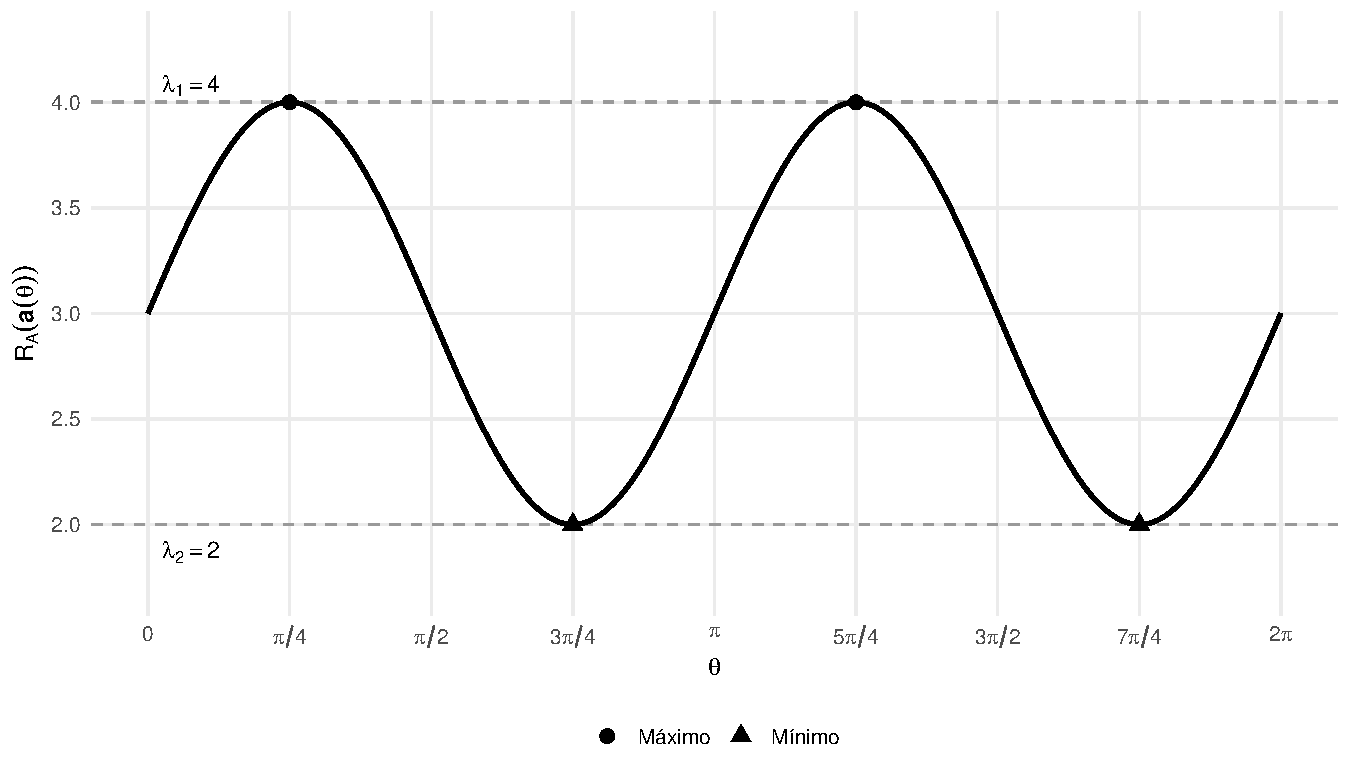
\includegraphics[keepaspectratio]{mod_1_autovetores_files/figure-pdf/fig-quociente-rayleigh-1.pdf}}

}

\caption{\label{fig-quociente-rayleigh}O quociente de Rayleigh assume
seus valores extremos nas direções dos autovetores associados aos
autovalores máximo e mínimo.}

\end{figure}%

As direções opostas representam a mesma reta e, por isso, produzem o
mesmo valor do quociente. Os máximos aparecem em duas posições angulares
separadas por \(\pi\), assim como os mínimos.

\subsection{Formulação com restrição de
norma}\label{formulauxe7uxe3o-com-restriuxe7uxe3o-de-norma}

A invariância à escala permite substituir o problema sobre vetores não
nulos por um problema sobre a esfera unitária:

\[
\max_{\mathbf{a}\neq\mathbf{0}}
\mathcal{R}_{\mathbf{A}}(\mathbf{a})
\]

é equivalente a

\[
\max_{\mathbf{a}}
\mathbf{a}^{\top}
\mathbf{A}
\mathbf{a},
\]

sujeito a

\[
\mathbf{a}^{\top}\mathbf{a}
=
1.
\]

A restrição de norma separa a escolha da \textbf{direção} da escolha da
magnitude do vetor. De fato,

\[
(c\mathbf{a})^{\top}
\mathbf{A}
(c\mathbf{a})
=
c^2
\mathbf{a}^{\top}
\mathbf{A}
\mathbf{a}.
\]

Portanto, sem uma normalização, o valor da forma quadrática pode ser
alterado simplesmente pelo escalonamento do vetor, mesmo quando sua
direção permanece a mesma.

Se existe uma direção para a qual

\[
\mathbf{a}^{\top}\mathbf{A}\mathbf{a}>0,
\]

o problema de maximização sem restrição é ilimitado superiormente.
Analogamente, se existe uma direção para a qual

\[
\mathbf{a}^{\top}\mathbf{A}\mathbf{a}<0,
\]

o problema de minimização sem restrição é ilimitado inferiormente.

A condição

\[
\mathbf{a}^{\top}\mathbf{a}=1
\]

elimina esse efeito de escala e restringe a otimização às direções
representadas por vetores unitários.

\subsection{Multiplicadores de
Lagrange}\label{multiplicadores-de-lagrange}

Em diferentes problemas da Estatística Multivariada, procura-se uma
\textbf{direção} no espaço das variáveis que torne máxima ou mínima
alguma quantidade de interesse. Essa quantidade pode representar, por
exemplo, variabilidade, separação entre grupos ou associação entre
conjuntos de variáveis.

Uma direção pode ser representada por um vetor \(\mathbf a\).
Entretanto, os vetores \(\mathbf a\) e \(c\mathbf a\), para \(c\neq 0\),
representam a mesma direção, embora tenham comprimentos diferentes. Por
isso, quando o interesse está apenas na direção, é conveniente impor a
normalização

\[
\mathbf a^{\top}\mathbf a=1.
\]

Essa restrição faz com que a busca seja realizada sobre o conjunto dos
vetores unitários. Geometricamente, em \(\mathbb R^p\), esses vetores
formam a esfera unitária.

Considere agora a forma quadrática

\[
f(\mathbf a)
=
\mathbf a^{\top}
\mathbf A
\mathbf a,
\]

em que \(\mathbf A\in\mathbb R^{p\times p}\) é simétrica. O problema
consiste em investigar como o valor de \(f(\mathbf a)\) varia quando a
direção \(\mathbf a\) percorre a esfera unitária.

\subsubsection{O que é um ponto estacionário sob uma
restrição?}\label{o-que-uxe9-um-ponto-estacionuxe1rio-sob-uma-restriuxe7uxe3o}

Em um problema sem restrições, um ponto estacionário de uma função
diferenciável é um ponto no qual seu gradiente é nulo. Em um problema
com restrição, essa condição precisa ser modificada, pois nem todas as
direções de deslocamento são permitidas.

Neste caso, \(\mathbf a\) deve permanecer sobre a esfera

\[
\mathbf a^{\top}\mathbf a=1.
\]

Um ponto é estacionário para o problema restrito quando pequenas
alterações de \(\mathbf a\) que respeitam essa restrição não produzem,
em primeira ordem, aumento ou redução da função objetivo.

Geometricamente, isso ocorre quando o gradiente da função objetivo não
possui componente na direção tangente à superfície da restrição. De
forma equivalente, o gradiente da função objetivo deve ser proporcional
ao gradiente da função que define a restrição.

Essa condição é obtida pelo método dos multiplicadores de Lagrange.

Considere a função lagrangiana

\[
\mathcal{L}
\left(
\mathbf{a},
\eta
\right)
=
\mathbf{a}^{\top}
\mathbf{A}
\mathbf{a}
-
\eta
\left(
\mathbf{a}^{\top}\mathbf{a}-1
\right),
\]

em que \(\eta\) é o multiplicador de Lagrange.

Como \(\mathbf{A}\) é simétrica,

\[
\nabla_{\mathbf{a}}
\left(
\mathbf{a}^{\top}
\mathbf{A}
\mathbf{a}
\right)
=
2\mathbf{A}\mathbf{a},
\]

e

\[
\nabla_{\mathbf{a}}
\left(
\mathbf{a}^{\top}\mathbf{a}
\right)
=
2\mathbf{a}.
\]

A condição de primeira ordem para um ponto estacionário é

\[
\nabla_{\mathbf{a}}
\mathcal{L}
=
\mathbf{0},
\]

isto é,

\[
2\mathbf{A}\mathbf{a}
-
2\eta\mathbf{a}
=
\mathbf{0}.
\]

Portanto,

\[
\mathbf{A}\mathbf{a}
=
\eta\mathbf{a}.
\]

Como a restrição

\[
\mathbf a^{\top}\mathbf a=1
\]

garante que \(\mathbf a\neq\mathbf 0\), essa equação mostra que as
direções estacionárias do problema são precisamente direções de
autovetores de \(\mathbf A\). O multiplicador de Lagrange \(\eta\) é o
autovalor associado à direção encontrada.

Multiplicando a equação

\[
\mathbf A\mathbf a
=
\eta\mathbf a
\]

à esquerda por \(\mathbf a^{\top}\), obtém-se

\[
\begin{aligned}
\mathbf a^{\top}\mathbf A\mathbf a
&=
\eta\mathbf a^{\top}\mathbf a\\
&=
\eta,
\end{aligned}
\]

pois \(\mathbf a^{\top}\mathbf a=1\).

Assim, quando \(\mathbf a\) é um autovetor unitário associado ao
autovalor \(\lambda\),

\[
\mathbf A\mathbf a
=
\lambda\mathbf a
\]

e

\[
\mathbf a^{\top}\mathbf A\mathbf a
=
\lambda.
\]

Portanto, há uma correspondência direta:

\[
\text{direção estacionária}
\longleftrightarrow
\text{autovetor}
\]

e

\[
\text{valor da forma quadrática nessa direção}
\longleftrightarrow
\text{autovalor}.
\]

Como \(\mathbf A\) é simétrica, seus autovalores são reais. Além disso,
pelos resultados do quociente de Rayleigh, para todo vetor unitário
\(\mathbf a\),

\[
\lambda_{\min}
\leq
\mathbf a^{\top}\mathbf A\mathbf a
\leq
\lambda_{\max}.
\]

Os extremos são atingidos nos autoespaços associados ao menor e ao maior
autovalor. Consequentemente,

\[
\max_{\mathbf a^{\top}\mathbf a=1}
\mathbf a^{\top}\mathbf A\mathbf a
=
\lambda_{\max},
\]

e

\[
\min_{\mathbf a^{\top}\mathbf a=1}
\mathbf a^{\top}\mathbf A\mathbf a
=
\lambda_{\min}.
\]

Assim:

\begin{itemize}
\tightlist
\item
  o maior autovalor fornece o máximo global da forma quadrática sobre a
  esfera unitária;
\item
  o menor autovalor fornece o mínimo global;
\item
  os demais autovalores correspondem a valores estacionários
  intermediários;
\item
  os autovetores associados fornecem as respectivas direções.
\end{itemize}

\begin{theorem}[Autovalores como valores
estacionários]\protect\hypertarget{thm-autovalores-otimizacao-restrita}{}\label{thm-autovalores-otimizacao-restrita}

Seja \(\mathbf{A}\in\mathbb{R}^{p\times p}\) uma matriz simétrica e
considere

\[
f(\mathbf a)
=
\mathbf a^{\top}\mathbf A\mathbf a
\]

restrita aos vetores que satisfazem

\[
\mathbf a^{\top}\mathbf a=1.
\]

Um vetor unitário \(\mathbf a\) é um ponto estacionário de \(f\) sobre a
esfera unitária se, e somente se, \(\mathbf a\) é um autovetor de
\(\mathbf A\).

Se

\[
\mathbf A\mathbf a
=
\lambda\mathbf a,
\]

então

\[
f(\mathbf a)
=
\mathbf a^{\top}\mathbf A\mathbf a
=
\lambda.
\]

Em particular, o maior autovalor corresponde ao máximo global da função
sobre a esfera unitária, e o menor autovalor corresponde ao mínimo
global.

\end{theorem}

Este resultado permite compreender por que autovalores e autovetores
surgem repetidamente em técnicas multivariadas. Em muitos casos, a
técnica procura uma direção \(\mathbf a\) que torne máxima uma
quantidade expressa por uma forma quadrática.

Na Análise de Componentes Principais, por exemplo, para um vetor
aleatório \(\mathbf X\) com matriz de covariâncias
\(\boldsymbol{\Sigma}\), a variância da combinação linear

\[
Y
=
\mathbf a^{\top}\mathbf X
\]

é

\[
\operatorname{Var}(Y)
=
\mathbf a^{\top}
\boldsymbol{\Sigma}
\mathbf a.
\]

A primeira componente principal procura a direção unitária que maximiza
essa variância:

\[
\max_{\mathbf a^{\top}\mathbf a=1}
\mathbf a^{\top}
\boldsymbol{\Sigma}
\mathbf a.
\]

Pelo resultado anterior, a solução é um autovetor associado ao maior
autovalor de \(\boldsymbol{\Sigma}\). Portanto,

\[
\text{maior autovalor}
\longrightarrow
\text{maior variância possível}
\]

e

\[
\text{autovetor correspondente}
\longrightarrow
\text{direção de maior variabilidade}.
\]

As componentes seguintes são obtidas acrescentando restrições de
ortogonalidade às direções já encontradas. Isso conduz sucessivamente
aos demais autovetores e autovalores.

A mesma estrutura reaparece, com modificações, em outros problemas
multivariados. Na análise discriminante, procura-se uma direção que
produza grande separação entre grupos em relação à variabilidade dentro
dos grupos. Na MANOVA, determinadas direções maximizam a variação
associada à hipótese em relação à variação residual. Na correlação
canônica, procuram-se combinações lineares de dois conjuntos de
variáveis que apresentem associação máxima.

Nesses casos, a função a ser otimizada envolve frequentemente uma razão
entre duas formas quadráticas,

\[
\frac{
\mathbf a^{\top}\mathbf A\mathbf a
}{
\mathbf a^{\top}\mathbf B\mathbf a
},
\]

e a condição de estacionariedade conduz ao problema de autovalores
generalizados

\[
\mathbf A\mathbf a
=
\lambda\mathbf B\mathbf a.
\]

Assim, autovalores e autovetores aparecem nessas técnicas porque
representam soluções de problemas de otimização sobre direções: os
autovetores fornecem as direções de interesse e os autovalores
quantificam o valor atingido pelo critério nessas direções.

\subsection{Direções sucessivas}\label{direuxe7uxf5es-sucessivas}

O problema de otimização anterior identifica uma direção associada ao
maior autovalor de \(\mathbf A\). Em muitas aplicações, entretanto,
interessa obter não apenas uma direção ótima, mas uma sequência de
direções que representem aspectos distintos da estrutura da matriz.

Depois de encontrar a primeira direção, pode-se procurar uma segunda
direção que maximize a mesma forma quadrática, mas que seja ortogonal à
primeira. O procedimento pode ser repetido sucessivamente, impondo que
cada nova direção seja ortogonal às anteriormente obtidas.

Considere

\[
\lambda_1
\geq
\lambda_2
\geq
\cdots
\geq
\lambda_p
\]

e uma base ortonormal de autovetores

\[
\mathbf{q}_1,\ldots,\mathbf{q}_p.
\]

O segundo problema é

\[
\max_{\mathbf{a}}
\mathbf{a}^{\top}
\mathbf{A}
\mathbf{a},
\]

sujeito a

\[
\mathbf{a}^{\top}\mathbf{a}=1
\]

e

\[
\mathbf{a}^{\top}\mathbf{q}_1=0.
\]

A restrição

\[
\mathbf a^{\top}\mathbf q_1=0
\]

impede que \(\mathbf a\) possua componente na direção de
\(\mathbf q_1\). Assim, se \(\mathbf a\) for escrito na base espectral,

\[
\mathbf a
=
z_1\mathbf q_1
+
z_2\mathbf q_2
+
\cdots
+
z_p\mathbf q_p,
\]

a condição de ortogonalidade implica

\[
z_1=0.
\]

Portanto, a otimização passa a ocorrer apenas no subespaço gerado por

\[
\mathbf q_2,\ldots,\mathbf q_p.
\]

Nesse subespaço, o maior autovalor disponível é \(\lambda_2\). Assim, o
maior valor da forma quadrática é \(\lambda_2\), atingido na direção de
\(\mathbf q_2\) quando \(\lambda_2\) é simples.

De forma geral, a \(k\)-ésima direção pode ser obtida por

\[
\max_{\mathbf{a}}
\mathbf{a}^{\top}
\mathbf{A}
\mathbf{a},
\]

sujeito a

\[
\mathbf{a}^{\top}\mathbf{a}=1
\]

e

\[
\mathbf{a}^{\top}\mathbf{q}_j=0,
\qquad
j=1,\ldots,k-1.
\]

\begin{theorem}[Caracterização variacional de direções
sucessivas]\protect\hypertarget{thm-caracterizacao-variacional-sucessiva}{}\label{thm-caracterizacao-variacional-sucessiva}

Seja \(\mathbf A\in\mathbb R^{p\times p}\) uma matriz simétrica, com
autovalores ordenados como

\[
\lambda_1
\geq
\lambda_2
\geq
\cdots
\geq
\lambda_p,
\]

e seja

\[
\mathbf q_1,\ldots,\mathbf q_p
\]

uma base ortonormal de autovetores correspondente a essa ordenação.
Então, para \(k=1,\ldots,p\),

\[
\lambda_k
=
\max_{
\substack{
\|\mathbf a\|=1\\
\mathbf a^{\top}\mathbf q_j=0,\;
j=1,\ldots,k-1
}
}
\mathbf a^{\top}\mathbf A\mathbf a.
\]

O máximo é atingido por \(\mathbf q_k\) e, quando \(\lambda_k\) possui
multiplicidade maior que \(1\), por qualquer autovetor unitário
associado a \(\lambda_k\) que satisfaça as restrições de ortogonalidade.
(Horn; Johnson, 2013)

\end{theorem}

\begin{proof}
Como

\[
\mathbf q_1,\ldots,\mathbf q_p
\]

formam uma base ortonormal de \(\mathbb R^p\), qualquer vetor
\(\mathbf a\) pode ser escrito como

\[
\mathbf a
=
\sum_{j=1}^{p}
z_j\mathbf q_j,
\]

em que

\[
z_j
=
\mathbf q_j^{\top}\mathbf a.
\]

As restrições

\[
\mathbf a^{\top}\mathbf q_j=0,
\qquad
j=1,\ldots,k-1,
\]

implicam

\[
z_1=\cdots=z_{k-1}=0.
\]

Portanto,

\[
\mathbf a
=
\sum_{j=k}^{p}
z_j\mathbf q_j.
\]

Como os autovetores são ortonormais e \(\|\mathbf a\|=1\),

\[
\sum_{j=k}^{p}z_j^2=1.
\]

Nas coordenadas espectrais,

\[
\begin{aligned}
\mathbf a^{\top}\mathbf A\mathbf a
&=
\sum_{j=k}^{p}
\lambda_jz_j^2.
\end{aligned}
\]

Como os autovalores estão ordenados de forma decrescente,

\[
\lambda_j\leq\lambda_k,
\qquad
j\geq k.
\]

Logo,

\[
\begin{aligned}
\mathbf a^{\top}\mathbf A\mathbf a
&=
\sum_{j=k}^{p}
\lambda_jz_j^2\\
&\leq
\lambda_k
\sum_{j=k}^{p}z_j^2\\
&=
\lambda_k.
\end{aligned}
\]

O limite é atingido tomando

\[
\mathbf a=\mathbf q_k,
\]

pois \(\mathbf q_k\) possui norma unitária, é ortogonal a
\(\mathbf q_1,\ldots,\mathbf q_{k-1}\) e satisfaz

\[
\mathbf A\mathbf q_k
=
\lambda_k\mathbf q_k.
\]

Assim,

\[
\mathbf q_k^{\top}\mathbf A\mathbf q_k
=
\lambda_k.
\]

Portanto,

\[
\max_{
\substack{
\|\mathbf a\|=1\\
\mathbf a^{\top}\mathbf q_j=0,\;
j=1,\ldots,k-1
}
}
\mathbf a^{\top}\mathbf A\mathbf a
=
\lambda_k.
\]
\end{proof}

Quando há autovalores repetidos, as direções individuais dentro do
autoespaço correspondente não são unicamente determinadas. Diferentes
bases ortonormais desse autoespaço produzem o mesmo valor da função
objetivo e representam o mesmo subespaço espectral. Assim, o subespaço
associado ao autovalor repetido é bem determinado, embora a escolha
particular dos autovetores que formam uma base desse subespaço não seja
única.

A caracterização variacional relaciona, portanto, três objetos
fundamentais:

\[
\text{forma quadrática}
\longleftrightarrow
\text{problema de otimização}
\longleftrightarrow
\text{estrutura espectral}.
\]

Além de identificar os valores extremos, essa caracterização permite
obter sucessivamente as direções ortogonais associadas aos autovalores
ordenados da matriz.

\section{Funções espectrais de
matrizes}\label{funuxe7uxf5es-espectrais-de-matrizes}

A decomposição espectral permite construir novas matrizes aplicando uma
função escalar aos autovalores. Esse procedimento fornece expressões
para potências, inversas, raízes quadradas, exponenciais, logaritmos e
pseudoinversas de matrizes simétricas.

Considere uma matriz simétrica

\[
\mathbf{A}
\in
\mathbb{R}^{p\times p}
\]

com decomposição espectral

\[
\mathbf{A}
=
\mathbf{Q}_{\mathbf{A}}
\boldsymbol{\Lambda}_{\mathbf{A}}
\mathbf{Q}_{\mathbf{A}}^{\top},
\]

em que

\[
\boldsymbol{\Lambda}_{\mathbf{A}}
=
\operatorname{diag}
\left(
\lambda_1,\ldots,\lambda_p
\right).
\]

Se \(f\) é uma função escalar real definida em todos os autovalores de
\(\mathbf{A}\), pode-se aplicá-la aos elementos diagonais:

\[
f
\left(
\boldsymbol{\Lambda}_{\mathbf{A}}
\right)
=
\operatorname{diag}
\left(
f(\lambda_1),\ldots,f(\lambda_p)
\right).
\]

\begin{definition}[Função espectral de uma matriz
simétrica]\protect\hypertarget{def-funcao-espectral}{}\label{def-funcao-espectral}

Seja

\[
\mathbf{A}
=
\mathbf{Q}_{\mathbf{A}}
\boldsymbol{\Lambda}_{\mathbf{A}}
\mathbf{Q}_{\mathbf{A}}^{\top}
\]

uma matriz simétrica e seja \(f\) uma função real definida no espectro
de \(\mathbf{A}\).

A \textbf{função espectral} \(f(\mathbf{A})\) é definida por

\[
f(\mathbf{A})
=
\mathbf{Q}_{\mathbf{A}}
f
\left(
\boldsymbol{\Lambda}_{\mathbf{A}}
\right)
\mathbf{Q}_{\mathbf{A}}^{\top}.
\]

\end{definition}

A definição não depende da base ortonormal escolhida dentro de um
autoespaço associado a um autovalor repetido.

De fato, considerando os autovalores distintos

\[
\lambda^{(1)},\ldots,\lambda^{(s)}
\]

e os respectivos projetores espectrais, a função também pode ser escrita
como

\[
f(\mathbf{A})
=
\sum_{h=1}^{s}
f
\left(
\lambda^{(h)}
\right)
\boldsymbol{\Pi}_{\lambda^{(h)}}.
\]

Os projetores são determinados pelos autoespaços, independentemente da
base ortonormal utilizada para representá-los.

\subsection{Ação sobre os
autoespaços}\label{auxe7uxe3o-sobre-os-autoespauxe7os}

\begin{proposition}[Ação de uma função
espectral]\protect\hypertarget{prp-funcao-espectral-autoespacos}{}\label{prp-funcao-espectral-autoespacos}

Se \(\mathbf{v}\) pertence ao autoespaço de \(\mathbf{A}\) associado ao
autovalor \(\lambda\), então

\[
f(\mathbf{A})\mathbf{v}
=
f(\lambda)\mathbf{v}.
\]

(Horn; Johnson, 1991)

\end{proposition}

\begin{proof}
Como

\[
\mathbf{A}\mathbf{v}
=
\lambda\mathbf{v},
\]

o vetor \(\mathbf{v}\) pertence à imagem do projetor

\[
\boldsymbol{\Pi}_{\lambda}
\]

e é anulado pelos projetores associados aos demais autovalores. Assim,

\[
\begin{aligned}
f(\mathbf{A})\mathbf{v}
&=
\sum_{h=1}^{s}
f
\left(
\lambda^{(h)}
\right)
\boldsymbol{\Pi}_{\lambda^{(h)}}
\mathbf{v}\\
&=
f(\lambda)\mathbf{v}.
\end{aligned}
\]
\end{proof}

Portanto, todo autovetor de \(\mathbf{A}\) associado a \(\lambda\)
também é autovetor de \(f(\mathbf{A})\), agora associado ao autovalor
\(f(\lambda)\). Mais geralmente, todo o autoespaço
\(\mathcal{E}_{\lambda}\) de \(\mathbf{A}\) permanece invariante sob
\(f(\mathbf{A})\).

A função pode fazer autovalores originalmente distintos assumirem o
mesmo valor. Se

\[
f(\lambda_i)
=
f(\lambda_j),
\]

os autoespaços correspondentes passam a pertencer ao mesmo autoespaço de
\(f(\mathbf{A})\). Por isso, \(f(\mathbf{A})\) pode possuir autoespaços
de dimensão maior que os autoespaços individuais de \(\mathbf{A}\).

\subsection{Potências inteiras}\label{potuxeancias-inteiras}

Para um inteiro \(k\geq0\), escolha

\[
f(\lambda)
=
\lambda^k.
\]

Então,

\[
\mathbf{A}^k
=
\mathbf{Q}_{\mathbf{A}}
\boldsymbol{\Lambda}_{\mathbf{A}}^k
\mathbf{Q}_{\mathbf{A}}^{\top},
\]

com

\[
\boldsymbol{\Lambda}_{\mathbf{A}}^k
=
\operatorname{diag}
\left(
\lambda_1^k,\ldots,\lambda_p^k
\right).
\]

Essa expressão coincide com a fórmula obtida pela diagonalização, mas a
ortogonalidade de \(\mathbf{Q}_{\mathbf{A}}\) fornece

\[
\mathbf{Q}_{\mathbf{A}}^{-1}
=
\mathbf{Q}_{\mathbf{A}}^{\top}.
\]

\begin{example}[Potência de uma matriz
simétrica]\protect\hypertarget{exm-potencia-espectral}{}\label{exm-potencia-espectral}

Considere

\[
\mathbf{A}
=
\begin{bmatrix}
3&1\\
1&3
\end{bmatrix},
\]

com decomposição espectral

\[
\mathbf{A}
=
\mathbf{Q}_{\mathbf{A}}
\begin{bmatrix}
4&0\\
0&2
\end{bmatrix}
\mathbf{Q}_{\mathbf{A}}^{\top}.
\]

Então,

\[
\mathbf{A}^2
=
\mathbf{Q}_{\mathbf{A}}
\begin{bmatrix}
16&0\\
0&4
\end{bmatrix}
\mathbf{Q}_{\mathbf{A}}^{\top}.
\]

Efetuando a multiplicação,

\[
\mathbf{A}^2
=
\begin{bmatrix}
10&6\\
6&10
\end{bmatrix}.
\]

A aplicação de \(\mathbf{A}\) duas vezes multiplica a componente na
direção de \(\mathbf{q}_1\) por

\[
4^2=16
\]

e a componente na direção de \(\mathbf{q}_2\) por

\[
2^2=4.
\]

\end{example}

\subsection{Inversa espectral}\label{inversa-espectral}

Se todos os autovalores são diferentes de zero, define-se

\[
f(\lambda)
=
\frac{1}{\lambda}.
\]

Nesse caso,

\[
\mathbf{A}^{-1}
=
\mathbf{Q}_{\mathbf{A}}
\boldsymbol{\Lambda}_{\mathbf{A}}^{-1}
\mathbf{Q}_{\mathbf{A}}^{\top},
\]

em que

\[
\boldsymbol{\Lambda}_{\mathbf{A}}^{-1}
=
\operatorname{diag}
\left(
\frac{1}{\lambda_1},
\ldots,
\frac{1}{\lambda_p}
\right).
\]

A inversa desfaz o escalonamento em cada direção espectral:

\[
\mathbf{A}^{-1}\mathbf{q}_j
=
\frac{1}{\lambda_j}
\mathbf{q}_j.
\]

Para o exemplo anterior,

\[
\mathbf{A}^{-1}
=
\mathbf{Q}_{\mathbf{A}}
\begin{bmatrix}
1/4&0\\
0&1/2
\end{bmatrix}
\mathbf{Q}_{\mathbf{A}}^{\top},
\]

o que resulta em

\[
\mathbf{A}^{-1}
=
\frac{1}{8}
\begin{bmatrix}
3&-1\\
-1&3
\end{bmatrix}.
\]

Se pelo menos um autovalor é igual a zero, a inversa usual não existe.

\subsection{Raiz quadrada principal}\label{raiz-quadrada-principal}

Para uma matriz semidefinida positiva, todos os autovalores são não
negativos. Assim, pode-se definir

\[
f(\lambda)
=
\sqrt{\lambda}.
\]

\begin{definition}[Raiz quadrada
principal]\protect\hypertarget{def-raiz-quadrada-principal}{}\label{def-raiz-quadrada-principal}

Se

\[
\mathbf{A}\succeq0,
\]

a raiz quadrada principal de \(\mathbf{A}\) é

\[
\mathbf{A}^{1/2}
=
\mathbf{Q}_{\mathbf{A}}
\boldsymbol{\Lambda}_{\mathbf{A}}^{1/2}
\mathbf{Q}_{\mathbf{A}}^{\top},
\]

em que

\[
\boldsymbol{\Lambda}_{\mathbf{A}}^{1/2}
=
\operatorname{diag}
\left(
\sqrt{\lambda_1},
\ldots,
\sqrt{\lambda_p}
\right).
\]

\end{definition}

A matriz \(\mathbf{A}^{1/2}\) é simétrica, semidefinida positiva e
satisfaz

\[
\mathbf{A}^{1/2}
\mathbf{A}^{1/2}
=
\mathbf{A}.
\]

Além disso, ela é a única matriz simétrica semidefinida positiva com
essa propriedade.

Para

\[
\mathbf{A}
=
\begin{bmatrix}
3&1\\
1&3
\end{bmatrix},
\]

tem-se

\[
\mathbf{A}^{1/2}
=
\mathbf{Q}_{\mathbf{A}}
\begin{bmatrix}
2&0\\
0&\sqrt{2}
\end{bmatrix}
\mathbf{Q}_{\mathbf{A}}^{\top}.
\]

Logo,

\[
\mathbf{A}^{1/2}
=
\frac{1}{2}
\begin{bmatrix}
2+\sqrt{2}&2-\sqrt{2}\\
2-\sqrt{2}&2+\sqrt{2}
\end{bmatrix}.
\]

A raiz quadrada principal multiplica as componentes espectrais por

\[
\sqrt{\lambda_j}.
\]

Aplicada duas vezes, ela produz o escalonamento original por
\(\lambda_j\).

\subsection{Raiz quadrada inversa}\label{raiz-quadrada-inversa}

Se

\[
\mathbf{A}\succ0,
\]

todos os autovalores são estritamente positivos. Define-se então

\[
\mathbf{A}^{-1/2}
=
\mathbf{Q}_{\mathbf{A}}
\boldsymbol{\Lambda}_{\mathbf{A}}^{-1/2}
\mathbf{Q}_{\mathbf{A}}^{\top},
\]

em que

\[
\boldsymbol{\Lambda}_{\mathbf{A}}^{-1/2}
=
\operatorname{diag}
\left(
\frac{1}{\sqrt{\lambda_1}},
\ldots,
\frac{1}{\sqrt{\lambda_p}}
\right).
\]

Como \(\mathbf{A}\succ0\), a raiz quadrada principal é invertível e

\[
\mathbf{A}^{-1/2}
=
\left(
\mathbf{A}^{1/2}
\right)^{-1}.
\]

Além disso,

\[
\mathbf{A}^{-1}
=
\mathbf{A}^{-1/2}
\mathbf{A}^{-1/2}
\]

e

\[
\mathbf{A}^{-1/2}
\mathbf{A}
\mathbf{A}^{-1/2}
=
\mathbf{I}_p.
\]

De fato,

\[
\begin{aligned}
\mathbf{A}^{-1/2}
\mathbf{A}
\mathbf{A}^{-1/2}
&=
\mathbf{Q}_{\mathbf{A}}
\boldsymbol{\Lambda}_{\mathbf{A}}^{-1/2}
\boldsymbol{\Lambda}_{\mathbf{A}}
\boldsymbol{\Lambda}_{\mathbf{A}}^{-1/2}
\mathbf{Q}_{\mathbf{A}}^{\top}\\
&=
\mathbf{Q}_{\mathbf{A}}
\mathbf{I}_p
\mathbf{Q}_{\mathbf{A}}^{\top}\\
&=
\mathbf{I}_p.
\end{aligned}
\]

A transformação

\[
\mathbf{z}
=
\mathbf{A}^{-1/2}\mathbf{x}
\]

reescalona as componentes espectrais de \(\mathbf{x}\) segundo os
fatores \(1/\sqrt{\lambda_j}\). Além disso, converte a forma quadrática
associada à inversa em uma norma euclidiana:

\[
\begin{aligned}
\mathbf{x}^{\top}
\mathbf{A}^{-1}
\mathbf{x}
&=
\mathbf{x}^{\top}
\mathbf{A}^{-1/2}
\mathbf{A}^{-1/2}
\mathbf{x}\\
&=
\mathbf{z}^{\top}\mathbf{z}\\
&=
\|\mathbf{z}\|^2.
\end{aligned}
\]

Quando \(\mathbf{A}\) for uma matriz de covariâncias
\(\boldsymbol{\Sigma}\succ0\), essa construção será retomada no
branqueamento. Para um vetor com média \(\boldsymbol{\mu}\), a
transformação correspondente será aplicada ao vetor centralizado,

\[
\mathbf{z}
=
\boldsymbol{\Sigma}^{-1/2}
\left(
\mathbf{x}-\boldsymbol{\mu}
\right).
\]

Nesse caso, a distância de Mahalanobis será interpretada como uma
distância euclidiana nas coordenadas branqueadas.

\subsection{Pseudoinversa espectral}\label{pseudoinversa-espectral}

Quando uma matriz possui autovalores nulos, não é possível inverter sua
ação em todas as direções. Ainda assim, é possível inverter os
escalonamentos nas direções associadas a autovalores não nulos.

\begin{definition}[Pseudoinversa de uma matriz
simétrica]\protect\hypertarget{def-pseudoinversa-espectral}{}\label{def-pseudoinversa-espectral}

Seja

\[
\mathbf{A}
=
\mathbf{Q}_{\mathbf{A}}
\boldsymbol{\Lambda}_{\mathbf{A}}
\mathbf{Q}_{\mathbf{A}}^{\top}
\]

uma matriz simétrica.

Define-se

\[
\lambda_j^{+}
=
\begin{cases}
1/\lambda_j,
&
\lambda_j\neq0,\\[4pt]
0,
&
\lambda_j=0.
\end{cases}
\]

A \textbf{pseudoinversa de Moore--Penrose} de \(\mathbf{A}\) é

\[
\mathbf{A}^{+}
=
\mathbf{Q}_{\mathbf{A}}
\boldsymbol{\Lambda}_{\mathbf{A}}^{+}
\mathbf{Q}_{\mathbf{A}}^{\top},
\]

em que

\[
\boldsymbol{\Lambda}_{\mathbf{A}}^{+}
=
\operatorname{diag}
\left(
\lambda_1^{+},
\ldots,
\lambda_p^{+}
\right).
\]

\end{definition}

A pseudoinversa atua separadamente sobre os autoespaços: nas direções
associadas a autovalores não nulos, aplica o fator \(1/\lambda\); no
autoespaço associado ao autovalor zero, sua ação é nula. Assim, ela
inverte a transformação sobre sua imagem e mantém eliminadas as
componentes pertencentes ao núcleo.

\begin{example}[Pseudoinversa de uma matriz
singular]\protect\hypertarget{exm-pseudoinversa-espectral}{}\label{exm-pseudoinversa-espectral}

Considere

\[
\mathbf{A}_0
=
\begin{bmatrix}
2&2\\
2&2
\end{bmatrix}.
\]

Seus autovalores são

\[
\lambda_1=4
\qquad
\text{e}
\qquad
\lambda_2=0,
\]

com autovetores unitários

\[
\mathbf{q}_1
=
\frac{1}{\sqrt{2}}
\begin{bmatrix}
1\\
1
\end{bmatrix}
\]

e

\[
\mathbf{q}_2
=
\frac{1}{\sqrt{2}}
\begin{bmatrix}
1\\
-1
\end{bmatrix}.
\]

A matriz \(\mathbf{A}_0\) não é invertível porque possui um autovalor
nulo. Para a pseudoinversa,

\[
\left(
\boldsymbol{\Lambda}_{\mathbf{A}_0}
\right)^{+}
=
\begin{bmatrix}
1/4&0\\
0&0
\end{bmatrix}.
\]

Portanto,

\[
\begin{aligned}
\mathbf{A}_0^{+}
&=
\mathbf{Q}_{\mathbf{A}_0}
\begin{bmatrix}
1/4&0\\
0&0
\end{bmatrix}
\mathbf{Q}_{\mathbf{A}_0}^{\top}\\
&=
\frac{1}{8}
\begin{bmatrix}
1&1\\
1&1
\end{bmatrix}.
\end{aligned}
\]

A componente na direção de \(\mathbf{q}_1\) é dividida por 4. A
componente na direção de \(\mathbf{q}_2\), pertencente ao núcleo de
\(\mathbf{A}_0\), é anulada.

\end{example}

Quando \(\mathbf{A}\) é invertível,

\[
\mathbf{A}^{+}
=
\mathbf{A}^{-1}.
\]

A pseudoinversa será retomada no capítulo seguinte, no qual será
definida para matrizes retangulares por meio da decomposição em valores
singulares.

\subsection{Exponencial e logaritmo
matriciais}\label{exponencial-e-logaritmo-matriciais}

A função exponencial é definida para qualquer matriz simétrica por

\[
\exp(\mathbf{A})
=
\mathbf{Q}_{\mathbf{A}}
\operatorname{diag}
\left(
e^{\lambda_1},
\ldots,
e^{\lambda_p}
\right)
\mathbf{Q}_{\mathbf{A}}^{\top}.
\]

Como

\[
e^{\lambda_j}>0,
\]

a matriz \(\exp(\mathbf{A})\) é positiva definida.

A exponencial matricial também pode ser representada pela série

\[
\exp(\mathbf{A})
=
\sum_{k=0}^{\infty}
\frac{\mathbf{A}^k}{k!}.
\]

Para uma matriz simétrica positiva definida, define-se o
\textbf{logaritmo principal} por

\[
\log(\mathbf{A})
=
\mathbf{Q}_{\mathbf{A}}
\operatorname{diag}
\left(
\log\lambda_1,
\ldots,
\log\lambda_p
\right)
\mathbf{Q}_{\mathbf{A}}^{\top}.
\]

As identidades escalares são preservadas espectralmente:

\[
\exp
\left(
\log(\mathbf{A})
\right)
=
\mathbf{A}
\]

para \(\mathbf{A}\succ0\), e

\[
\log
\left(
\exp(\mathbf{A})
\right)
=
\mathbf{A}
\]

para toda matriz simétrica real.

A Tabela~\ref{tbl-funcoes-espectrais} reúne as principais funções
desenvolvidas nesta seção.

\begin{longtable}[]{@{}
  >{\raggedright\arraybackslash}p{(\linewidth - 4\tabcolsep) * \real{0.3333}}
  >{\raggedright\arraybackslash}p{(\linewidth - 4\tabcolsep) * \real{0.3333}}
  >{\raggedright\arraybackslash}p{(\linewidth - 4\tabcolsep) * \real{0.3333}}@{}}
\caption{Principais funções espectrais de matrizes
simétricas.}\label{tbl-funcoes-espectrais}\tabularnewline
\toprule\noalign{}
\begin{minipage}[b]{\linewidth}\raggedright
Função
\end{minipage} & \begin{minipage}[b]{\linewidth}\raggedright
Ação sobre \(\lambda_j\)
\end{minipage} & \begin{minipage}[b]{\linewidth}\raggedright
Condição adicional
\end{minipage} \\
\midrule\noalign{}
\endfirsthead
\toprule\noalign{}
\begin{minipage}[b]{\linewidth}\raggedright
Função
\end{minipage} & \begin{minipage}[b]{\linewidth}\raggedright
Ação sobre \(\lambda_j\)
\end{minipage} & \begin{minipage}[b]{\linewidth}\raggedright
Condição adicional
\end{minipage} \\
\midrule\noalign{}
\endhead
\bottomrule\noalign{}
\endlastfoot
\(\mathbf{A}^k\) & \(\lambda_j^k\) & \(k\in\{0,1,2,\ldots\}\) \\
\(\mathbf{A}^{-1}\) & \(1/\lambda_j\) & \(\lambda_j\neq0\) para todo
\(j\) \\
\(\mathbf{A}^{1/2}\) & \(\sqrt{\lambda_j}\) & \(\mathbf{A}\succeq0\) \\
\(\mathbf{A}^{-1/2}\) & \(1/\sqrt{\lambda_j}\) & \(\mathbf{A}\succ0\) \\
\(\mathbf{A}^{+}\) & \(1/\lambda_j\) se \(\lambda_j\neq0\); \(0\) se
\(\lambda_j=0\) & nenhuma além da simetria assumida na seção \\
\(\exp(\mathbf{A})\) & \(e^{\lambda_j}\) & nenhuma além da simetria
assumida na seção \\
\(\log(\mathbf{A})\) & \(\log\lambda_j\) & \(\mathbf{A}\succ0\) \\
\end{longtable}

As funções espectrais atuam separadamente sobre os autoespaços,
transformando cada autovalor \(\lambda\) no valor escalar
\(f(\lambda)\). Essa construção permite obter diretamente potências,
inversas, raízes e pseudoinversas e mostra como certas transformações
matriciais podem ser compreendidas como reescalonamentos das direções
espectrais.

Em particular, a raiz quadrada e a raiz quadrada inversa permitem
converter problemas definidos por uma geometria induzida por uma matriz
positiva definida em problemas euclidianos equivalentes. Essa ideia será
utilizada imediatamente na formulação dos autovalores generalizados.

\section{Aprofundamento: autovalores
generalizados}\label{aprofundamento-autovalores-generalizados}

\begin{tcolorbox}[enhanced jigsaw, colback=white, breakable, bottomrule=.15mm, left=2mm, arc=.35mm, rightrule=.15mm, colframe=quarto-callout-note-color-frame, toprule=.15mm, leftrule=.75mm, opacityback=0]

\vspace{-3mm}\textbf{Leitura de aprofundamento}\vspace{3mm}

Esta seção apresenta uma extensão do problema ordinário de autovalores
para situações em que duas formas quadráticas são consideradas
simultaneamente. Embora esse desenvolvimento não seja necessário para
acompanhar os resultados centrais da decomposição espectral, ele fornece
uma base matemática importante para técnicas multivariadas que envolvem
a comparação entre diferentes estruturas de variabilidade, separação ou
associação.

Ao longo da seção, serão apresentados os autovalores generalizados, o
quociente de Rayleigh generalizado, a ortogonalidade em uma métrica
definida por uma matriz positiva definida e a redução do problema
generalizado a um problema espectral ordinário.

\end{tcolorbox}

Alguns problemas de Estatística Multivariada envolvem a comparação entre
duas formas quadráticas, em vez da otimização de uma única forma
quadrática relativamente à norma euclidiana. Nesses casos, surge
naturalmente o problema de autovalores generalizados,

\[
\mathbf A\mathbf v
=
\lambda
\mathbf M\mathbf v,
\]

em que \(\mathbf A\) é simétrica e \(\mathbf M\) é simétrica positiva
definida.

Essa estrutura generaliza o problema ordinário de autovalores,
recuperado quando

\[
\mathbf M=\mathbf I_p.
\]

Os autovalores generalizados serão úteis posteriormente em problemas que
envolvem a comparação entre diferentes medidas de variabilidade,
separação ou associação. A leitura a seguir desenvolve a formulação
matemática desse problema e sua relação com o quociente de Rayleigh e a
decomposição espectral.

O quociente de Rayleigh compara uma forma quadrática com a norma
euclidiana do vetor. Em outros problemas, a normalização também é
definida por uma forma quadrática:

\[
\mathbf{a}^{\top}
\mathbf{M}
\mathbf{a},
\]

em que

\[
\mathbf{M}
=
\mathbf{M}^{\top}
\succ0.
\]

Conforme a Definição~\ref{def-produto-interno-induzido}, a matriz
\(\mathbf{M}\) determina o produto interno

\[
\left\langle
\mathbf{x},
\mathbf{y}
\right\rangle_{\mathbf{M}}
=
\mathbf{x}^{\top}
\mathbf{M}
\mathbf{y}
\]

e a norma

\[
\|\mathbf{x}\|_{\mathbf{M}}
=
\sqrt{
\mathbf{x}^{\top}
\mathbf{M}
\mathbf{x}
}.
\]

Nesse contexto, procura-se uma direção que compare as formas quadráticas
associadas a duas matrizes.

\begin{definition}[Autovalor e autovetor
generalizados]\protect\hypertarget{def-autovalor-generalizado}{}\label{def-autovalor-generalizado}

Sejam

\[
\mathbf{A},
\mathbf{M}
\in
\mathbb{R}^{p\times p},
\]

com

\[
\mathbf{A}
=
\mathbf{A}^{\top}
\]

e

\[
\mathbf{M}
=
\mathbf{M}^{\top}
\succ0.
\]

Um escalar real

\[
\lambda\in\mathbb{R}
\]

é um \textbf{autovalor generalizado} do par \((\mathbf{A},\mathbf{M})\)
quando existe um vetor não nulo

\[
\mathbf{v}\in\mathbb{R}^p
\]

tal que

\[
\mathbf{A}\mathbf{v}
=
\lambda
\mathbf{M}\mathbf{v}.
\]

O vetor \(\mathbf{v}\) é denominado \textbf{autovetor generalizado}
associado a \(\lambda\).

\end{definition}

Quando

\[
\mathbf{M}
=
\mathbf{I}_p,
\]

recupera-se o problema ordinário:

\[
\mathbf{A}\mathbf{v}
=
\lambda\mathbf{v}.
\]

A equação generalizada pode ser reorganizada como

\[
\left(
\mathbf{A}
-
\lambda\mathbf{M}
\right)
\mathbf{v}
=
\mathbf{0}.
\]

Existem soluções não triviais se, e somente se,

\[
\det
\left(
\mathbf{A}
-
\lambda\mathbf{M}
\right)
=
0.
\]

Essa equação é a equação característica generalizada do par
\((\mathbf{A},\mathbf{M})\) e determina seus autovalores generalizados.

\subsection{Quociente de Rayleigh
generalizado}\label{quociente-de-rayleigh-generalizado}

\begin{definition}[Quociente de Rayleigh
generalizado]\protect\hypertarget{def-quociente-rayleigh-generalizado}{}\label{def-quociente-rayleigh-generalizado}

Sejam \(\mathbf A\in\mathbb R^{p\times p}\) simétrica e
\(\mathbf M\in\mathbb R^{p\times p}\) simétrica positiva definida. Para
\(\mathbf a\in\mathbb R^p\), com \(\mathbf a\neq\mathbf0\), o
\textbf{quociente de Rayleigh generalizado} associado ao par
\((\mathbf A,\mathbf M)\) é

\[
\mathcal R_{\mathbf A,\mathbf M}(\mathbf a)
=
\frac{
\mathbf a^{\top}\mathbf A\mathbf a
}{
\mathbf a^{\top}\mathbf M\mathbf a
}
=
\frac{
q_{\mathbf A}(\mathbf a)
}{
\|\mathbf a\|_{\mathbf M}^2
}.
\]

O numerador é a forma quadrática associada a \(\mathbf A\), enquanto o
denominador é o quadrado da norma induzida por \(\mathbf M\),

\[
\|\mathbf a\|_{\mathbf M}^2
=
\left\langle
\mathbf a,\mathbf a
\right\rangle_{\mathbf M}
=
\mathbf a^{\top}\mathbf M\mathbf a.
\]

\end{definition}

Como \(\mathbf M\succ\mathbf0\),

\[
\mathbf a^{\top}\mathbf M\mathbf a
>
0
\]

para todo \(\mathbf a\neq\mathbf0\). Portanto, o denominador é sempre
positivo e o quociente está definido para todo vetor não nulo.

No quociente de Rayleigh ordinário, a normalização é realizada pela
norma euclidiana,

\[
\|\mathbf a\|^2
=
\mathbf a^{\top}\mathbf a.
\]

No caso generalizado, essa normalização é substituída pela norma
induzida por \(\mathbf M\). Assim, o comprimento do vetor passa a ser
medido segundo a geometria determinada por essa matriz.

Assim como no caso ordinário, o quociente é invariante à escala. Para
qualquer escalar \(c\neq0\),

\[
\begin{aligned}
\mathcal R_{\mathbf A,\mathbf M}(c\mathbf a)
&=
\frac{
(c\mathbf a)^{\top}\mathbf A(c\mathbf a)
}{
(c\mathbf a)^{\top}\mathbf M(c\mathbf a)
}\\
&=
\frac{
c^2\mathbf a^{\top}\mathbf A\mathbf a
}{
c^2\mathbf a^{\top}\mathbf M\mathbf a
}\\
&=
\mathcal R_{\mathbf A,\mathbf M}(\mathbf a).
\end{aligned}
\]

Portanto, o valor do quociente depende da direção determinada por
\(\mathbf a\), e não de sua magnitude segundo a norma induzida por
\(\mathbf M\).

Essa invariância permite escolher, em cada direção, um representante com
norma unitária na geometria determinada por \(\mathbf M\).
Consequentemente, o problema

\[
\max_{\mathbf a\neq\mathbf0}
\mathcal R_{\mathbf A,\mathbf M}(\mathbf a)
\]

é equivalente a

\[
\max_{\mathbf a}
\mathbf a^{\top}\mathbf A\mathbf a,
\]

sujeito a

\[
\mathbf a^{\top}\mathbf M\mathbf a
=
1.
\]

A restrição equivale a

\[
\|\mathbf a\|_{\mathbf M}=1
\]

e, portanto, fixa o comprimento de \(\mathbf a\) segundo a geometria
induzida por \(\mathbf M\).

Para determinar os pontos estacionários desse problema restrito,
considere a função lagrangiana

\[
\mathcal L(\mathbf a,\eta)
=
\mathbf a^{\top}\mathbf A\mathbf a
-
\eta
\left(
\mathbf a^{\top}\mathbf M\mathbf a
-
1
\right),
\]

em que \(\eta\) é o multiplicador de Lagrange.

Como \(\mathbf A\) e \(\mathbf M\) são simétricas,

\[
\nabla_{\mathbf a}
\left(
\mathbf a^{\top}\mathbf A\mathbf a
\right)
=
2\mathbf A\mathbf a
\]

e

\[
\nabla_{\mathbf a}
\left(
\mathbf a^{\top}\mathbf M\mathbf a
\right)
=
2\mathbf M\mathbf a.
\]

Assim,

\[
\nabla_{\mathbf a}\mathcal L
=
2\mathbf A\mathbf a
-
2\eta\mathbf M\mathbf a.
\]

A condição de primeira ordem

\[
\nabla_{\mathbf a}\mathcal L
=
\mathbf0
\]

produz

\[
\mathbf A\mathbf a
=
\eta\mathbf M\mathbf a.
\]

Como a restrição

\[
\mathbf a^{\top}\mathbf M\mathbf a=1
\]

garante que \(\mathbf a\neq\mathbf0\), essa equação mostra que todo
ponto estacionário \(\mathbf a\) é um autovetor generalizado do par
\((\mathbf A,\mathbf M)\) e que o multiplicador \(\eta\) é o autovalor
generalizado correspondente.

Multiplicando a equação

\[
\mathbf A\mathbf a
=
\eta\mathbf M\mathbf a
\]

à esquerda por \(\mathbf a^{\top}\), obtém-se

\[
\mathbf a^{\top}\mathbf A\mathbf a
=
\eta
\mathbf a^{\top}\mathbf M\mathbf a.
\]

Sob a normalização

\[
\mathbf a^{\top}\mathbf M\mathbf a
=
1,
\]

segue que

\[
\mathbf a^{\top}\mathbf A\mathbf a
=
\eta.
\]

Além disso,

\[
\mathcal R_{\mathbf A,\mathbf M}(\mathbf a)
=
\frac{
\mathbf a^{\top}\mathbf A\mathbf a
}{
\mathbf a^{\top}\mathbf M\mathbf a
}
=
\eta.
\]

Portanto, em um autovetor generalizado normalizado, o valor do quociente
de Rayleigh generalizado coincide com o autovalor generalizado
correspondente.

\subsection{Redução a um problema espectral
ordinário}\label{reduuxe7uxe3o-a-um-problema-espectral-ordinuxe1rio}

Como \(\mathbf{M}\succ0\), a matriz \(\mathbf{M}\) é invertível, e a
equação generalizada também poderia ser escrita como

\[
\mathbf{M}^{-1}
\mathbf{A}
\mathbf{v}
=
\lambda\mathbf{v}.
\]

Entretanto, mesmo que \(\mathbf{A}\) e \(\mathbf{M}\) sejam simétricas,
a matriz \(\mathbf{M}^{-1}\mathbf{A}\) não precisa ser simétrica. Para
preservar a estrutura simétrica e poder aplicar diretamente o Teorema
Espectral, é preferível transformar o problema utilizando a raiz
quadrada de \(\mathbf{M}\).

Como \(\mathbf{M}\succ0\), existem as matrizes simétricas

\[
\mathbf{M}^{1/2}
\]

e

\[
\mathbf{M}^{-1/2}.
\]

Defina

\[
\mathbf{u}
=
\mathbf{M}^{1/2}\mathbf{v}.
\]

Consequentemente,

\[
\mathbf{v}
=
\mathbf{M}^{-1/2}\mathbf{u}.
\]

Substituindo na equação generalizada,

\[
\mathbf{A}
\mathbf{M}^{-1/2}
\mathbf{u}
=
\lambda
\mathbf{M}
\mathbf{M}^{-1/2}
\mathbf{u}.
\]

Como

\[
\mathbf{M}
\mathbf{M}^{-1/2}
=
\mathbf{M}^{1/2},
\]

obtém-se

\[
\mathbf{A}
\mathbf{M}^{-1/2}
\mathbf{u}
=
\lambda
\mathbf{M}^{1/2}
\mathbf{u}.
\]

Multiplicando à esquerda por \(\mathbf{M}^{-1/2}\),

\[
\left(
\mathbf{M}^{-1/2}
\mathbf{A}
\mathbf{M}^{-1/2}
\right)
\mathbf{u}
=
\lambda\mathbf{u}.
\]

Defina

\[
\widetilde{\mathbf{A}}
=
\mathbf{M}^{-1/2}
\mathbf{A}
\mathbf{M}^{-1/2}.
\]

Como \(\mathbf{A}\) e \(\mathbf{M}^{-1/2}\) são simétricas,

\[
\widetilde{\mathbf{A}}^{\top}
=
\widetilde{\mathbf{A}}.
\]

Assim, o problema generalizado é convertido no problema espectral
ordinário

\[
\widetilde{\mathbf{A}}\mathbf{u}
=
\lambda\mathbf{u},
\]

para uma matriz simétrica. Consequentemente, todos os autovalores
generalizados do par \((\mathbf{A},\mathbf{M})\) são reais e os
resultados do Teorema Espectral podem ser aplicados à matriz
\(\widetilde{\mathbf{A}}\).

Essa transformação também converte o quociente generalizado em um
quociente ordinário. Como

\[
\mathbf{a}
=
\mathbf{M}^{-1/2}\mathbf{u},
\]

tem-se

\[
\begin{aligned}
\mathbf{a}^{\top}
\mathbf{M}
\mathbf{a}
&=
\mathbf{u}^{\top}
\mathbf{M}^{-1/2}
\mathbf{M}
\mathbf{M}^{-1/2}
\mathbf{u}\\
&=
\mathbf{u}^{\top}\mathbf{u}
\end{aligned}
\]

e

\[
\begin{aligned}
\mathbf{a}^{\top}
\mathbf{A}
\mathbf{a}
&=
\mathbf{u}^{\top}
\mathbf{M}^{-1/2}
\mathbf{A}
\mathbf{M}^{-1/2}
\mathbf{u}\\
&=
\mathbf{u}^{\top}
\widetilde{\mathbf{A}}
\mathbf{u}.
\end{aligned}
\]

Portanto,

\[
\mathcal{R}_{\mathbf{A},\mathbf{M}}(\mathbf{a})
=
\mathcal{R}_{\widetilde{\mathbf{A}}}(\mathbf{u}).
\]

A mudança de variáveis

\[\mathbf{u}=\mathbf{M}^{1/2}\mathbf{a}\]

transforma a geometria induzida por \(\mathbf{M}\) em geometria
euclidiana, pois

\[
\mathbf{a}^{\top}
\mathbf{M}
\mathbf{a}
=
\mathbf{u}^{\top}\mathbf{u}.
\]

Equivalentemente,

\[
\mathbf{a}
=
\mathbf{M}^{-1/2}\mathbf{u}.
\]

Geometricamente, \(\mathbf{M}^{-1/2}\) transforma a esfera unitária
euclidiana no elipsoide

\[
\left\{
\mathbf{a}\in\mathbb{R}^p:
\mathbf{a}^{\top}\mathbf{M}\mathbf{a}=1
\right\}.
\]

O problema generalizado pode, portanto, ser estudado como um problema de
Rayleigh ordinário no sistema de coordenadas em que a métrica definida
por \(\mathbf{M}\) se torna euclidiana.

Quando \(\mathbf{M}\) representar posteriormente uma matriz de
covariâncias, essa mesma estrutura estará relacionada ao branqueamento.
Aqui, porém, \(\mathbf{M}\) representa genericamente a matriz que define
a geometria do problema.

\begin{theorem}[Extremos do quociente de Rayleigh
generalizado]\protect\hypertarget{thm-extremos-rayleigh-generalizado}{}\label{thm-extremos-rayleigh-generalizado}

Sejam \(\mathbf{A}\) simétrica e \(\mathbf{M}\) positiva definida.
Denote por

\[
\lambda_1
\geq
\cdots
\geq
\lambda_p
\]

os autovalores generalizados do par \((\mathbf{A},\mathbf{M})\).

Então, para todo \(\mathbf{a}\neq\mathbf{0}\),

\[
\lambda_p
\leq
\mathcal{R}_{\mathbf{A},\mathbf{M}}(\mathbf{a})
\leq
\lambda_1.
\]

Além disso,

\[
\max_{\mathbf{a}\neq\mathbf{0}}
\mathcal{R}_{\mathbf{A},\mathbf{M}}(\mathbf{a})
=
\lambda_1
\]

e

\[
\min_{\mathbf{a}\neq\mathbf{0}}
\mathcal{R}_{\mathbf{A},\mathbf{M}}(\mathbf{a})
=
\lambda_p.
\]

O máximo é atingido por todo vetor não nulo do autoespaço generalizado
associado a \(\lambda_1\), e o mínimo é atingido por todo vetor não nulo
do autoespaço generalizado associado a \(\lambda_p\).

\end{theorem}

\begin{proof}
A transformação

\[
\mathbf{u}
=
\mathbf{M}^{1/2}\mathbf{a}
\]

é invertível e estabelece

\[
\mathcal{R}_{\mathbf{A},\mathbf{M}}(\mathbf{a})
=
\mathcal{R}_{\widetilde{\mathbf{A}}}(\mathbf{u}),
\]

em que

\[
\widetilde{\mathbf{A}}
=
\mathbf{M}^{-1/2}
\mathbf{A}
\mathbf{M}^{-1/2}
\]

é simétrica.

Os autovalores ordinários de \(\widetilde{\mathbf{A}}\) são os
autovalores generalizados do par \((\mathbf{A},\mathbf{M})\). Aplicando
o Teorema~\ref{thm-extremos-quociente-rayleigh} a
\(\widetilde{\mathbf{A}}\), obtêm-se os limites e os extremos
apresentados.
\end{proof}

\subsection{\texorpdfstring{Ortogonalidade na métrica de
\(\mathbf{M}\)}{Ortogonalidade na métrica de \textbackslash mathbf\{M\}}}\label{ortogonalidade-na-muxe9trica-de-mathbfm}

Os autovetores generalizados não precisam ser ortogonais segundo o
produto interno euclidiano. Eles podem, entretanto, ser escolhidos
ortonormais na geometria determinada por \(\mathbf{M}\).

\begin{proposition}[Ortogonalidade e base de autovetores
generalizados]\protect\hypertarget{prp-ortogonalidade-autovetores-generalizados}{}\label{prp-ortogonalidade-autovetores-generalizados}

Sejam \(\mathbf{A}\) simétrica e \(\mathbf{M}\succ0\).

Se \(\mathbf{v}_i\) e \(\mathbf{v}_j\) são autovetores generalizados
associados a autovalores distintos \(\lambda_i\) e \(\lambda_j\), então

\[
\mathbf{v}_i^{\top}
\mathbf{M}
\mathbf{v}_j
=
0.
\]

Além disso, existe uma base de \(\mathbb{R}^p\) formada por autovetores
generalizados

\[
\mathcal{B}_g
=
\{
\mathbf{v}_1,\ldots,\mathbf{v}_p
\}
\]

que pode ser escolhida de modo que

\[
\mathbf{v}_i^{\top}
\mathbf{M}
\mathbf{v}_j
=
\delta_{ij}.
\]

(Horn; Johnson, 2013)

\end{proposition}

\begin{proof}
Para autovalores distintos,

\[
\mathbf{A}\mathbf{v}_i
=
\lambda_i
\mathbf{M}\mathbf{v}_i
\]

e

\[
\mathbf{A}\mathbf{v}_j
=
\lambda_j
\mathbf{M}\mathbf{v}_j.
\]

Como \(\mathbf{A}\) é simétrica,

\[
\begin{aligned}
\lambda_i
\mathbf{v}_i^{\top}
\mathbf{M}
\mathbf{v}_j
&=
\left(
\mathbf{A}\mathbf{v}_i
\right)^{\top}
\mathbf{v}_j\\
&=
\mathbf{v}_i^{\top}
\mathbf{A}^{\top}
\mathbf{v}_j\\
&=
\mathbf{v}_i^{\top}
\mathbf{A}
\mathbf{v}_j\\
&=
\lambda_j
\mathbf{v}_i^{\top}
\mathbf{M}
\mathbf{v}_j.
\end{aligned}
\]

Portanto,

\[
\left(
\lambda_i-\lambda_j
\right)
\mathbf{v}_i^{\top}
\mathbf{M}
\mathbf{v}_j
=
0.
\]

Como \(\lambda_i\neq\lambda_j\),

\[
\mathbf{v}_i^{\top}
\mathbf{M}
\mathbf{v}_j
=
0.
\]

Para mostrar a existência de uma base completa, considere

\[
\widetilde{\mathbf{A}}
=
\mathbf{M}^{-1/2}
\mathbf{A}
\mathbf{M}^{-1/2}.
\]

Como \(\widetilde{\mathbf{A}}\) é simétrica, o Teorema Espectral garante
uma base ortonormal de autovetores

\[
\{
\mathbf{u}_1,\ldots,\mathbf{u}_p
\}.
\]

Defina

\[
\mathbf{v}_j
=
\mathbf{M}^{-1/2}
\mathbf{u}_j.
\]

Esses vetores são autovetores generalizados e

\[
\begin{aligned}
\mathbf{v}_i^{\top}
\mathbf{M}
\mathbf{v}_j
&=
\mathbf{u}_i^{\top}
\mathbf{M}^{-1/2}
\mathbf{M}
\mathbf{M}^{-1/2}
\mathbf{u}_j\\
&=
\mathbf{u}_i^{\top}\mathbf{u}_j\\
&=
\delta_{ij}.
\end{aligned}
\]

Assim, mesmo quando há autovalores generalizados repetidos, pode-se
escolher uma base ortonormal segundo o produto interno induzido por
\(\mathbf{M}\).
\end{proof}

\subsection{Diagonalização simultânea por
congruência}\label{diagonalizauxe7uxe3o-simultuxe2nea-por-congruuxeancia}

Considere a decomposição espectral

\[
\widetilde{\mathbf{A}}
=
\mathbf{Q}_{g}
\boldsymbol{\Lambda}_{g}
\mathbf{Q}_{g}^{\top},
\]

em que

\[
\widetilde{\mathbf{A}}
=
\mathbf{M}^{-1/2}
\mathbf{A}
\mathbf{M}^{-1/2}.
\]

Defina

\[
\mathbf{B}_{g}
=
\mathbf{M}^{-1/2}
\mathbf{Q}_{g}.
\]

Como \(\mathbf{M}^{-1/2}\) é invertível e \(\mathbf{Q}_g\) é ortogonal,
\(\mathbf{B}_g\) é invertível. Suas colunas formam uma base
\(\mathbf{M}\)-ortonormal de autovetores generalizados.

De fato,

\[
\begin{aligned}
\mathbf{A}\mathbf{B}_{g}
&=
\mathbf{A}
\mathbf{M}^{-1/2}
\mathbf{Q}_{g}\\
&=
\mathbf{M}^{1/2}
\widetilde{\mathbf{A}}
\mathbf{Q}_{g}\\
&=
\mathbf{M}^{1/2}
\mathbf{Q}_{g}
\boldsymbol{\Lambda}_{g}\\
&=
\mathbf{M}
\mathbf{B}_{g}
\boldsymbol{\Lambda}_{g}.
\end{aligned}
\]

Além disso,

\[
\begin{aligned}
\mathbf{B}_{g}^{\top}
\mathbf{M}
\mathbf{B}_{g}
&=
\mathbf{Q}_{g}^{\top}
\mathbf{M}^{-1/2}
\mathbf{M}
\mathbf{M}^{-1/2}
\mathbf{Q}_{g}\\
&=
\mathbf{Q}_{g}^{\top}
\mathbf{Q}_{g}\\
&=
\mathbf{I}_p,
\end{aligned}
\]

e

\[
\begin{aligned}
\mathbf{B}_{g}^{\top}
\mathbf{A}
\mathbf{B}_{g}
&=
\mathbf{Q}_{g}^{\top}
\mathbf{M}^{-1/2}
\mathbf{A}
\mathbf{M}^{-1/2}
\mathbf{Q}_{g}\\
&=
\mathbf{Q}_{g}^{\top}
\widetilde{\mathbf{A}}
\mathbf{Q}_{g}\\
&=
\boldsymbol{\Lambda}_{g}.
\end{aligned}
\]

Portanto,

\[
\mathbf{B}_{g}^{\top}
\mathbf{M}
\mathbf{B}_{g}
=
\mathbf{I}_p
\]

e

\[
\mathbf{B}_{g}^{\top}
\mathbf{A}
\mathbf{B}_{g}
=
\boldsymbol{\Lambda}_{g}.
\]

O par \((\mathbf{A},\mathbf{M})\) é, assim, reduzido simultaneamente por
uma transformação de congruência:

\[
(\mathbf{A},\mathbf{M})
\longrightarrow
(
\boldsymbol{\Lambda}_g,
\mathbf{I}_p
).
\]

Essa operação deve ser distinguida da semelhança

\[
\mathbf{B}^{-1}
\mathbf{A}
\mathbf{B},
\]

utilizada para representar um único operador em outra base. Na
congruência, as matrizes aparecem multiplicadas pela transposta da
matriz de base à esquerda e pela própria matriz à direita.

Como

\[
\mathbf{B}_{g}^{\top}
\mathbf{M}
\mathbf{B}_{g}
=
\mathbf{I}_p,
\]

segue que

\[
\mathbf{B}_{g}^{-1}
=
\mathbf{B}_{g}^{\top}
\mathbf{M}.
\]

Assim, se

\[
\mathbf{a}
=
\mathbf{B}_{g}\mathbf{z},
\]

então as coordenadas de \(\mathbf a\) nessa base são

\[
\mathbf{z}
=
\mathbf{B}_{g}^{-1}\mathbf{a}
=
\mathbf{B}_{g}^{\top}
\mathbf{M}
\mathbf{a}.
\]

Nessas coordenadas,

\[
\mathbf{a}^{\top}
\mathbf{M}
\mathbf{a}
=
\mathbf{z}^{\top}\mathbf{z}
\]

e

\[
\mathbf{a}^{\top}
\mathbf{A}
\mathbf{a}
=
\mathbf{z}^{\top}
\boldsymbol{\Lambda}_{g}
\mathbf{z}.
\]

Consequentemente,

\[
\mathcal{R}_{\mathbf{A},\mathbf{M}}(\mathbf{a})
=
\frac{
\sum_{j=1}^{p}\lambda_jz_j^2
}{
\sum_{j=1}^{p}z_j^2
}.
\]

O quociente generalizado assume, portanto, a mesma forma do quociente de
Rayleigh ordinário quando expresso na base \(\mathbf{M}\)-ortonormal de
autovetores generalizados.

\begin{example}[Autovalores generalizados de duas formas
quadráticas]\protect\hypertarget{exm-autovalores-generalizados}{}\label{exm-autovalores-generalizados}

Considere

\[
\mathbf{A}
=
\begin{bmatrix}
5&1\\
1&2
\end{bmatrix}
\]

e

\[
\mathbf{M}
=
\begin{bmatrix}
2&0\\
0&1
\end{bmatrix}.
\]

As duas matrizes são simétricas e \(\mathbf{M}\) é positiva definida.

Os autovalores generalizados são obtidos por

\[
\det
\left(
\mathbf{A}
-
\lambda\mathbf{M}
\right)
=
0.
\]

Como

\[
\mathbf{A}
-
\lambda\mathbf{M}
=
\begin{bmatrix}
5-2\lambda&1\\
1&2-\lambda
\end{bmatrix},
\]

tem-se

\[
\begin{aligned}
\det
\left(
\mathbf{A}
-
\lambda\mathbf{M}
\right)
&=
(5-2\lambda)(2-\lambda)-1\\
&=
2\lambda^2-9\lambda+9\\
&=
(2\lambda-3)(\lambda-3).
\end{aligned}
\]

Portanto,

\[
\lambda_1=3
\]

e

\[
\lambda_2
=
\frac{3}{2}.
\]

Para \(\lambda_1=3\),

\[
\mathbf{A}
-
3\mathbf{M}
=
\begin{bmatrix}
-1&1\\
1&-1
\end{bmatrix}.
\]

O sistema fornece

\[
v_2=v_1,
\]

de modo que um autovetor generalizado é

\[
\mathbf{v}_1
=
\begin{bmatrix}
1\\
1
\end{bmatrix}.
\]

De fato,

\[
\mathbf{A}\mathbf{v}_1
=
\begin{bmatrix}
6\\
3
\end{bmatrix}
\]

e

\[
3\mathbf{M}\mathbf{v}_1
=
3
\begin{bmatrix}
2\\
1
\end{bmatrix}
=
\begin{bmatrix}
6\\
3
\end{bmatrix}.
\]

Para

\[
\lambda_2
=
\frac{3}{2},
\]

tem-se

\[
\mathbf{A}
-
\frac{3}{2}\mathbf{M}
=
\begin{bmatrix}
2&1\\
1&1/2
\end{bmatrix}.
\]

O sistema conduz a

\[
v_2=-2v_1.
\]

Assim, pode-se escolher

\[
\mathbf{v}_2
=
\begin{bmatrix}
1\\
-2
\end{bmatrix}.
\]

Esses vetores não são ortogonais no produto interno euclidiano:

\[
\mathbf{v}_1^{\top}\mathbf{v}_2
=
-1.
\]

Entretanto,

\[
\begin{aligned}
\mathbf{v}_1^{\top}
\mathbf{M}
\mathbf{v}_2
&=
\begin{bmatrix}
1&1
\end{bmatrix}
\begin{bmatrix}
2&0\\
0&1
\end{bmatrix}
\begin{bmatrix}
1\\
-2
\end{bmatrix}\\
&=
0.
\end{aligned}
\]

Logo, eles são ortogonais na geometria determinada por \(\mathbf{M}\).

Suas normas nessa métrica são

\[
\|\mathbf{v}_1\|_{\mathbf{M}}
=
\sqrt{3}
\]

e

\[
\|\mathbf{v}_2\|_{\mathbf{M}}
=
\sqrt{6}.
\]

Os autovetores generalizados normalizados são

\[
\mathbf{b}_{g,1}
=
\frac{1}{\sqrt{3}}
\begin{bmatrix}
1\\
1
\end{bmatrix}
\]

e

\[
\mathbf{b}_{g,2}
=
\frac{1}{\sqrt{6}}
\begin{bmatrix}
1\\
-2
\end{bmatrix}.
\]

Reunindo-os nas colunas da matriz da base

\[
\mathbf{B}_{g}
=
\begin{bmatrix}
\mathbf{b}_{g,1}&
\mathbf{b}_{g,2}
\end{bmatrix},
\]

obtêm-se

\[
\mathbf{B}_{g}^{\top}
\mathbf{M}
\mathbf{B}_{g}
=
\mathbf{I}_2
\]

e

\[
\mathbf{B}_{g}^{\top}
\mathbf{A}
\mathbf{B}_{g}
=
\begin{bmatrix}
3&0\\
0&3/2
\end{bmatrix}.
\]

O maior valor da razão

\[
\frac{
\mathbf{a}^{\top}
\mathbf{A}
\mathbf{a}
}{
\mathbf{a}^{\top}
\mathbf{M}
\mathbf{a}
}
\]

é 3 e ocorre no autoespaço generalizado gerado por \(\mathbf{v}_1\). O
menor valor é \(3/2\) e ocorre no autoespaço generalizado gerado por
\(\mathbf{v}_2\).

\end{example}

Os autovalores generalizados permitem comparar duas formas quadráticas
em uma geometria definida por uma delas. Essa estrutura será utilizada
posteriormente em problemas que comparam diferentes fontes de dispersão
ou associação, sem antecipar aqui a formulação específica dessas
técnicas.

\section{Síntese do capítulo}\label{suxedntese-do-capuxedtulo-4}

Este capítulo desenvolveu a estrutura espectral das transformações
lineares quadradas. O ponto de partida foi a identificação de direções
invariantes, isto é, direções nas quais a ação de uma matriz reduz-se à
multiplicação por um escalar.

Para

\[\mathbf{A}\mathbf{v}=\lambda\mathbf{v},\]

com \(\mathbf{v}\neq\mathbf{0}\), o escalar \(\lambda\) é um autovalor e
\(\mathbf{v}\) é um autovetor correspondente. O conjunto formado pelo
vetor nulo e por todos os autovetores associados a \(\lambda\) constitui
o autoespaço

\[
\mathcal{E}_{\lambda}
=
\mathcal{N}
\left(
\mathbf{A}
-
\lambda\mathbf{I}_p
\right).
\]

Os autovalores são determinados pela condição

\[
\det
\left(
\mathbf{A}
-
\lambda\mathbf{I}_p
\right)
=
0.
\]

A multiplicidade algébrica \(m_a(\lambda)\) registra a multiplicidade de
\(\lambda\) como raiz do polinômio característico, enquanto a
multiplicidade geométrica

\[
m_g(\lambda)
=
\dim
\left(
\mathcal{E}_{\lambda}
\right)
\]

mede a dimensão do autoespaço correspondente.

Quando \(\mathbf{A}\) possui \(p\) autovetores linearmente
independentes, eles formam uma base

\[
\mathcal{B}_{\mathbf{A}}
=
\{
\mathbf{v}_1,\ldots,\mathbf{v}_p
\},
\]

cuja matriz é

\[
\mathbf{B}_{\mathbf{A}}
=
\begin{bmatrix}
\mathbf{v}_1&
\cdots&
\mathbf{v}_p
\end{bmatrix}.
\]

Nessa base,

\[
[T_{\mathbf{A}}]_{\mathcal{B}_{\mathbf{A}}\leftarrow\mathcal{B}_{\mathbf{A}}}
=
\mathbf{B}_{\mathbf{A}}^{-1}
\mathbf{A}
\mathbf{B}_{\mathbf{A}}
=
\boldsymbol{\Lambda}_{\mathbf{A}},
\]

e, portanto,

\[
\mathbf{A}
=
\mathbf{B}_{\mathbf{A}}
\boldsymbol{\Lambda}_{\mathbf{A}}
\mathbf{B}_{\mathbf{A}}^{-1}.
\]

A diagonalização é, assim, uma mudança para coordenadas nas quais o
operador atua separadamente sobre cada direção da base de autovetores.

Para matrizes simétricas reais, o Teorema Espectral garante uma base
ortonormal de autovetores. Nesse caso, a matriz da base pode ser
escolhida ortogonal,

\[
\mathbf{Q}_{\mathbf{A}}
=
\begin{bmatrix}
\mathbf{q}_1&
\cdots&
\mathbf{q}_p
\end{bmatrix},
\]

com

\[
\mathbf{Q}_{\mathbf{A}}^{-1}
=
\mathbf{Q}_{\mathbf{A}}^{\top},
\]

e obtém-se a decomposição espectral

\[
\mathbf{A}
=
\mathbf{Q}_{\mathbf{A}}
\boldsymbol{\Lambda}_{\mathbf{A}}
\mathbf{Q}_{\mathbf{A}}^{\top}.
\]

Equivalentemente,

\[
\mathbf{A}
=
\sum_{j=1}^{p}
\lambda_j
\mathbf{q}_j
\mathbf{q}_j^{\top}.
\]

Agrupando autovalores repetidos, essa representação pode ser escrita em
termos dos projetores espectrais:

\[
\mathbf{A}
=
\sum_{h}
\lambda^{(h)}
\boldsymbol{\Pi}_{\lambda^{(h)}}.
\]

Essa forma mostra que uma matriz simétrica atua projetando o vetor sobre
autoespaços ortogonais e aplicando a cada componente o autovalor
correspondente.

A decomposição espectral também permite recuperar diretamente
propriedades da matriz:

\[
\operatorname{tr}(\mathbf{A})
=
\sum_{j=1}^{p}\lambda_j,
\]

\[
\det(\mathbf{A})
=
\prod_{j=1}^{p}\lambda_j,
\]

e

\[
\operatorname{posto}(\mathbf{A})
=
\#\{j:\lambda_j\neq0\},
\]

contando as multiplicidades.

Além disso,

\[
\ker(T_{\mathbf{A}})
=
\mathcal{N}(\mathbf{A})
=
\operatorname{span}
\left\{
\mathbf{q}_j:
\lambda_j=0
\right\},
\]

enquanto

\[
\operatorname{Im}(T_{\mathbf{A}})
=
\mathcal{C}(\mathbf{A})
=
\operatorname{span}
\left\{
\mathbf{q}_j:
\lambda_j\neq0
\right\}.
\]

Para matrizes simétricas,

\[
\operatorname{Im}(T_{\mathbf{A}})
=
\ker(T_{\mathbf{A}})^{\perp}.
\]

A mesma decomposição simplifica as formas quadráticas. Se

\[
\mathbf{z}
=
[\mathbf{x}]_{\mathcal{B}_{\mathbf{A}}}
=
\mathbf{Q}_{\mathbf{A}}^{\top}\mathbf{x},
\]

então

\[
\mathbf{x}^{\top}
\mathbf{A}
\mathbf{x}
=
\sum_{j=1}^{p}
\lambda_jz_j^2.
\]

As possibilidades de sinal da forma quadrática são, portanto,
determinadas pelos sinais dos autovalores. Quando \(\mathbf{A}\succ0\),
suas superfícies de nível são elipsoides cujos eixos estão alinhados aos
autovetores.

O quociente de Rayleigh,

\[
\mathcal{R}_{\mathbf{A}}(\mathbf{a})
=
\frac{
\mathbf{a}^{\top}
\mathbf{A}
\mathbf{a}
}{
\mathbf{a}^{\top}\mathbf{a}
},
\]

é uma média ponderada dos autovalores. Para

\[
\lambda_1
\geq
\lambda_2
\geq
\cdots
\geq
\lambda_p,
\]

tem-se

\[
\lambda_p
\leq
\mathcal{R}_{\mathbf{A}}(\mathbf{a})
\leq
\lambda_1.
\]

O máximo e o mínimo são atingidos nos autoespaços associados aos
autovalores extremos. A otimização de uma forma quadrática sob a
restrição

\[
\mathbf{a}^{\top}\mathbf{a}=1
\]

conduz à condição

\[
\mathbf{A}\mathbf{a}
=
\lambda\mathbf{a}.
\]

Autovalores e autovetores podem, portanto, ser interpretados também como
valores e direções estacionárias de problemas de otimização quadrática.

A decomposição espectral permite ainda definir funções de matrizes
simétricas. Se \(f\) está definida no espectro de \(\mathbf{A}\),

\[
f(\mathbf{A})
=
\mathbf{Q}_{\mathbf{A}}
f
\left(
\boldsymbol{\Lambda}_{\mathbf{A}}
\right)
\mathbf{Q}_{\mathbf{A}}^{\top}.
\]

Equivalentemente,

\[
f(\mathbf{A})
=
\sum_h
f
\left(
\lambda^{(h)}
\right)
\boldsymbol{\Pi}_{\lambda^{(h)}}.
\]

Assim, a função espectral preserva os autoespaços e transforma cada
autovalor \(\lambda\) no escalar \(f(\lambda)\). Potências, inversas,
raízes quadradas, raízes quadradas inversas, pseudoinversas,
exponenciais e logaritmos são casos particulares dessa construção, sob
as condições necessárias à definição de cada função.

Quando a geometria do problema é determinada por uma matriz simétrica
positiva definida \(\mathbf{M}\), surge o problema de autovalores
generalizados

\[
\mathbf{A}\mathbf{v}
=
\lambda
\mathbf{M}\mathbf{v},
\]

com \(\mathbf{A}=\mathbf{A}^{\top}\) e \(\mathbf{M}\succ0\).

O quociente correspondente é

\[
\mathcal{R}_{\mathbf{A},\mathbf{M}}(\mathbf{a})
=
\frac{
\mathbf{a}^{\top}
\mathbf{A}
\mathbf{a}
}{
\mathbf{a}^{\top}
\mathbf{M}
\mathbf{a}
}.
\]

A transformação

\[
\mathbf{u}
=
\mathbf{M}^{1/2}\mathbf{a}
\]

converte esse problema em um problema de Rayleigh ordinário para a
matriz simétrica

\[
\widetilde{\mathbf{A}}
=
\mathbf{M}^{-1/2}
\mathbf{A}
\mathbf{M}^{-1/2}.
\]

Consequentemente, os autovalores generalizados são reais e pode-se
escolher uma base de autovetores generalizados cuja matriz
\(\mathbf{B}_g\) satisfaz

\[
\mathbf{B}_g^{\top}
\mathbf{M}
\mathbf{B}_g
=
\mathbf{I}_p
\]

e

\[
\mathbf{B}_g^{\top}
\mathbf{A}
\mathbf{B}_g
=
\boldsymbol{\Lambda}_g.
\]

A Tabela~\ref{tbl-sintese-espectral} reúne as expressões principais
desenvolvidas no capítulo.

\begin{longtable}[]{@{}
  >{\raggedright\arraybackslash}p{(\linewidth - 4\tabcolsep) * \real{0.3333}}
  >{\raggedright\arraybackslash}p{(\linewidth - 4\tabcolsep) * \real{0.3333}}
  >{\raggedright\arraybackslash}p{(\linewidth - 4\tabcolsep) * \real{0.3333}}@{}}
\caption{Síntese dos principais objetos espectrais desenvolvidos no
capítulo.}\label{tbl-sintese-espectral}\tabularnewline
\toprule\noalign{}
\begin{minipage}[b]{\linewidth}\raggedright
Objeto
\end{minipage} & \begin{minipage}[b]{\linewidth}\raggedright
Expressão
\end{minipage} & \begin{minipage}[b]{\linewidth}\raggedright
Interpretação
\end{minipage} \\
\midrule\noalign{}
\endfirsthead
\toprule\noalign{}
\begin{minipage}[b]{\linewidth}\raggedright
Objeto
\end{minipage} & \begin{minipage}[b]{\linewidth}\raggedright
Expressão
\end{minipage} & \begin{minipage}[b]{\linewidth}\raggedright
Interpretação
\end{minipage} \\
\midrule\noalign{}
\endhead
\bottomrule\noalign{}
\endlastfoot
Equação de autovalor & \(\mathbf{A}\mathbf{v}=\lambda\mathbf{v}\) &
Identifica direções invariantes \\
Autoespaço &
\(\mathcal{E}_{\lambda}=\mathcal{N}(\mathbf{A}-\lambda\mathbf{I}_p)\) &
Reúne os vetores associados a \(\lambda\) \\
Diagonalização &
\(\mathbf{A}=\mathbf{B}_{\mathbf{A}}\boldsymbol{\Lambda}_{\mathbf{A}}\mathbf{B}_{\mathbf{A}}^{-1}\)
& Representa o operador em uma base de autovetores \\
Decomposição espectral &
\(\mathbf{A}=\mathbf{Q}_{\mathbf{A}}\boldsymbol{\Lambda}_{\mathbf{A}}\mathbf{Q}_{\mathbf{A}}^{\top}\)
& Diagonaliza ortogonalmente uma matriz simétrica \\
Projetor espectral &
\(\boldsymbol{\Pi}_{\lambda}=\mathbf{Q}_{\lambda}\mathbf{Q}_{\lambda}^{\top}\)
& Projeta sobre o autoespaço associado a \(\lambda\) \\
Forma quadrática &
\(\mathbf{x}^{\top}\mathbf{A}\mathbf{x}=\sum_j\lambda_jz_j^2\) & Separa
as contribuições das direções espectrais \\
Quociente de Rayleigh &
\(\mathcal{R}_{\mathbf{A}}(\mathbf{a})=\dfrac{\mathbf{a}^{\top}\mathbf{A}\mathbf{a}}{\mathbf{a}^{\top}\mathbf{a}}\)
& Caracteriza valores e direções espectrais por otimização \\
Função espectral &
\(f(\mathbf{A})=\mathbf{Q}_{\mathbf{A}}f(\boldsymbol{\Lambda}_{\mathbf{A}})\mathbf{Q}_{\mathbf{A}}^{\top}\)
& Aplica uma função aos autovalores \\
Problema generalizado &
\(\mathbf{A}\mathbf{v}=\lambda\mathbf{M}\mathbf{v}\) & Compara duas
formas quadráticas \\
Base generalizada &
\(\mathbf{B}_g^{\top}\mathbf{M}\mathbf{B}_g=\mathbf{I}_p\) & Define
ortonormalidade na geometria induzida por \(\mathbf{M}\) \\
Diagonalização por congruência &
\(\mathbf{B}_g^{\top}\mathbf{A}\mathbf{B}_g=\boldsymbol{\Lambda}_g\) &
Reduz simultaneamente as duas formas quadráticas \\
\end{longtable}

Ao final deste capítulo, o estudante deverá ser capaz de:

\begin{itemize}
\tightlist
\item
  identificar autovalores, autovetores e autoespaços e interpretar seu
  significado geométrico;
\item
  distinguir multiplicidades algébrica e geométrica;
\item
  determinar quando uma matriz é diagonalizável;
\item
  interpretar a diagonalização como mudança para uma base de
  autovetores;
\item
  aplicar o Teorema Espectral a matrizes simétricas reais;
\item
  interpretar projetores e subespaços espectrais;
\item
  relacionar autovalores a traço, determinante, posto, núcleo, imagem e
  positividade;
\item
  representar formas quadráticas em coordenadas espectrais;
\item
  formular problemas de otimização por meio do quociente de Rayleigh;
\item
  construir e interpretar funções espectrais de matrizes;
\item
  compreender inversas, raízes e pseudoinversas pela ação sobre os
  autovalores;
\item
  formular e transformar problemas de autovalores generalizados;
\item
  distinguir ortogonalidade euclidiana de ortogonalidade segundo uma
  matriz positiva definida.
\end{itemize}

A decomposição espectral fornece uma descrição particularmente simples
para matrizes simétricas quadradas. Entretanto, matrizes de dados e
muitas transformações de interesse são retangulares ou não simétricas e,
portanto, não admitem diretamente essa decomposição. O próximo capítulo
amplia essas ideias por meio da \textbf{Decomposição em Valores
Singulares}, relacionando matrizes retangulares aos espectros de
\(\mathbf{A}^{\top}\mathbf{A}\) e \(\mathbf{A}\mathbf{A}^{\top}\) e
conectando valores singulares, espaços fundamentais, posto e
aproximações de baixa dimensão.

\chapter{Decomposição em Valores
Singulares}\label{decomposiuxe7uxe3o-em-valores-singulares}

No capítulo anterior, a decomposição espectral foi utilizada para
representar uma matriz simétrica real na forma

\[
\mathbf{A}
=
\mathbf{Q}_{\mathbf{A}}
\boldsymbol{\Lambda}_{\mathbf{A}}
\mathbf{Q}_{\mathbf{A}}^{\top}.
\]

Essa representação identifica uma base ortonormal de autovetores na qual
a transformação atua separadamente sobre cada coordenada. A decomposição
espectral ortogonal, entretanto, depende da simetria da matriz e é
formulada para operadores cujo domínio e contradomínio possuem a mesma
dimensão.

Em Análise Multivariada, um dos objetos mais frequentes é a matriz de
dados

\[
\mathbf{X}
\in
\mathbb{R}^{n\times p},
\]

cujas linhas representam observações e colunas representam variáveis. Em
geral,

\[
n\neq p,
\]

de modo que \(\mathbf{X}\) é retangular. Mesmo quando uma matriz é
quadrada, ela pode não ser simétrica nem possuir uma base ortonormal de
autovetores.

A \textbf{Decomposição em Valores Singulares}, ou SVD, fornece uma
representação aplicável a qualquer matriz real. Para uma transformação

\[
T_{\mathbf{A}}:
\mathbb{R}^{p}
\longrightarrow
\mathbb{R}^{q},
\qquad
T_{\mathbf{A}}(\mathbf{x})
=
\mathbf{A}\mathbf{x},
\]

a SVD relaciona duas bases ortonormais:

\begin{itemize}
\tightlist
\item
  uma base do espaço de origem \(\mathbb{R}^{p}\);
\item
  uma base do espaço de chegada \(\mathbb{R}^{q}\).
\end{itemize}

A transformação associa determinadas direções dessas duas bases e
multiplica os comprimentos por fatores não negativos denominados
\textbf{valores singulares}.

Essa representação permite descrever:

\begin{itemize}
\tightlist
\item
  o posto da matriz;
\item
  os espaços das linhas e das colunas;
\item
  o núcleo e o núcleo da transposta;
\item
  os fatores máximos e mínimos de alteração dos comprimentos;
\item
  aproximações de posto reduzido;
\item
  a pseudoinversa;
\item
  soluções de mínimos quadrados.
\end{itemize}

A SVD também estabelece uma ligação entre os espaços das observações e
das variáveis de uma matriz de dados. Essa dualidade será utilizada
posteriormente na formulação de métodos de redução de dimensionalidade e
de representação de estruturas matriciais.

\begin{tcolorbox}[enhanced jigsaw, colback=white, breakable, bottomrule=.15mm, left=2mm, arc=.35mm, rightrule=.15mm, colframe=quarto-callout-note-color-frame, toprule=.15mm, leftrule=.75mm, opacityback=0]

\vspace{-3mm}\textbf{Convenções de notação}\vspace{3mm}

Ao longo deste capítulo:

\begin{itemize}
\tightlist
\item
  \(\mathbf{A}\in\mathbb{R}^{q\times p}\) representa uma matriz real e
  \(T_{\mathbf{A}}:\mathbb{R}^p\to\mathbb{R}^q\) a transformação linear
  associada;
\item
  \(r=\operatorname{posto}(\mathbf{A})\) representa o posto de
  \(\mathbf{A}\);
\item
  \(d_1\geq\cdots\geq d_r>0\) representam os valores singulares
  positivos de \(\mathbf{A}\);
\item
  \(\mathbf{v}_j\in\mathbb{R}^p\) representa um vetor singular à
  direita;
\item
  \(\mathbf{u}_j\in\mathbb{R}^q\) representa um vetor singular à
  esquerda;
\item
  \(\mathbf{U}\), \(\mathbf{D}\) e \(\mathbf{V}\) representam os fatores
  da SVD completa;
\item
  \(\mathbf{U}_r\), \(\mathbf{D}_r\) e \(\mathbf{V}_r\) representam os
  fatores da SVD compacta;
\item
  \(\mathbf{U}_k\), \(\mathbf{D}_k\) e \(\mathbf{V}_k\) representam os
  fatores de uma SVD truncada;
\item
  \(\mathbf{A}^{+}\) representa a pseudoinversa de Moore--Penrose;
\item
  \(\|\mathbf{A}\|_2\) e \(\|\mathbf{A}\|_F\) representam,
  respectivamente, as normas espectral e de Frobenius.
\end{itemize}

As convenções estabelecidas nos capítulos anteriores para núcleo,
imagem, espaço coluna, espaço linha e bases ortonormais permanecem
válidas.

\end{tcolorbox}

\section{Definição e formas da Decomposição em Valores
Singulares}\label{definiuxe7uxe3o-e-formas-da-decomposiuxe7uxe3o-em-valores-singulares}

Considere uma matriz real

\[
\mathbf{A}
\in
\mathbb{R}^{q\times p},
\]

que representa uma transformação de \(\mathbb{R}^{p}\) em
\(\mathbb{R}^{q}\).

A matriz pode ser retangular, quadrada, simétrica ou não simétrica.
Nenhuma hipótese de invertibilidade ou de posto completo é necessária
para a existência da SVD.

\begin{theorem}[Existência da Decomposição em Valores
Singulares]\protect\hypertarget{thm-existencia-svd}{}\label{thm-existencia-svd}

Para toda matriz

\[
\mathbf{A}
\in
\mathbb{R}^{q\times p},
\]

existem matrizes ortogonais

\[
\mathbf{U}
\in
\mathbb{R}^{q\times q}
\]

e

\[
\mathbf{V}
\in
\mathbb{R}^{p\times p},
\]

e uma matriz diagonal retangular

\[
\mathbf{D}
\in
\mathbb{R}^{q\times p}
\]

tais que

\[
\mathbf{A}
=
\mathbf{U}
\mathbf{D}
\mathbf{V}^{\top}.
\]

As matrizes ortogonais satisfazem

\[
\mathbf{U}^{\top}\mathbf{U}
=
\mathbf{U}\mathbf{U}^{\top}
=
\mathbf{I}_q
\]

e

\[
\mathbf{V}^{\top}\mathbf{V}
=
\mathbf{V}\mathbf{V}^{\top}
=
\mathbf{I}_p.
\]

Os elementos diagonais não negativos de \(\mathbf{D}\) podem ser
ordenados como

\[
d_1
\geq
d_2
\geq
\cdots
\geq
d_{\min(q,p)}
\geq
0.
\]

Esses elementos são os \textbf{valores singulares} de \(\mathbf{A}\).
(Golub; Van Loan, 2013)

\end{theorem}

A demonstração será apresentada posteriormente, após a construção da SVD
a partir das decomposições espectrais de \(\mathbf{A}^{\top}\mathbf{A}\)
e \(\mathbf{A}\mathbf{A}^{\top}\).

\begin{definition}[Matriz diagonal
retangular]\protect\hypertarget{def-matriz-diagonal-retangular}{}\label{def-matriz-diagonal-retangular}

Seja

\[
\mathbf D
\in
\mathbb R^{q\times p}
\]

e defina

\[
s
=
\min(q,p).
\]

A matriz \(\mathbf D\) é denominada \textbf{diagonal retangular} quando
existem escalares

\[
d_1,\ldots,d_s
\]

tais que

\[
D_{ij}
=
\begin{cases}
d_i, & i=j\leq s,\\
0, & \text{caso contrário}.
\end{cases}
\]

Assim, apenas os elementos da diagonal principal podem ser diferentes de
zero.

No bloco diagonal de ordem \(s\), essa condição pode ser escrita de
forma compacta utilizando a delta de Kronecker:

\[
D_{ij}
=
d_i\delta_{ij},
\qquad
i,j=1,\ldots,s.
\]

\end{definition}

Se

\[
q>p,
\]

então \(s=p\) e \(\mathbf D\) possui \(q-p\) linhas nulas abaixo de sua
parte diagonal.

Se

\[
p>q,
\]

então \(s=q\) e \(\mathbf D\) possui \(p-q\) colunas nulas à direita de
sua parte diagonal.

Por exemplo, quando \(q>p\),

\[
\mathbf{D}
=
\begin{bmatrix}
d_1 & 0 & \cdots & 0\\
0 & d_2 & \cdots & 0\\
\vdots & \vdots & \ddots & \vdots\\
0 & 0 & \cdots & d_p\\
0 & 0 & \cdots & 0\\
\vdots & \vdots & & \vdots\\
0 & 0 & \cdots & 0
\end{bmatrix}
\in
\mathbb{R}^{q\times p}.
\]

Nesse caso, a parte diagonal possui \(p=\min(q,p)\) elementos e as
\(q-p\) linhas restantes são nulas.

Quando \(p>q\),

\[
\mathbf{D}
=
\begin{bmatrix}
d_1 & 0 & \cdots & 0 & 0 & \cdots & 0\\
0 & d_2 & \cdots & 0 & 0 & \cdots & 0\\
\vdots & \vdots & \ddots & \vdots & \vdots & & \vdots\\
0 & 0 & \cdots & d_q & 0 & \cdots & 0
\end{bmatrix}
\in
\mathbb{R}^{q\times p}.
\]

Agora, a parte diagonal possui \(q=\min(q,p)\) elementos e as \(p-q\)
colunas restantes são nulas.

Como

\[
s
=
\min(q,p),
\]

a matriz \(\mathbf D\) possui \(s\) posições diagonais. Se

\[
r
=
\operatorname{posto}(\mathbf A),
\]

então exatamente \(r\) valores singulares são positivos. Ordenando-os de
forma decrescente,

\[
d_1
\geq
d_2
\geq
\cdots
\geq
d_r
>
0,
\]

enquanto, quando \(r<s\),

\[
d_{r+1}
=
\cdots
=
d_s
=
0.
\]

Assim, o número de valores singulares positivos é exatamente o posto de
\(\mathbf A\) e, consequentemente, a dimensão da imagem da transformação
linear associada:

\[
r
=
\operatorname{posto}(\mathbf A)
=
\dim
\left(
\operatorname{Im}(T_{\mathbf A})
\right).
\]

\subsection{Vetores singulares}\label{vetores-singulares}

Escreva as matrizes ortogonais como

\[
\mathbf{U}
=
\begin{bmatrix}
\mathbf{u}_1&
\cdots&
\mathbf{u}_q
\end{bmatrix}
\]

e

\[
\mathbf{V}
=
\begin{bmatrix}
\mathbf{v}_1&
\cdots&
\mathbf{v}_p
\end{bmatrix}.
\]

\begin{definition}[Valores e vetores
singulares]\protect\hypertarget{def-vetores-valores-singulares}{}\label{def-vetores-valores-singulares}

Na decomposição

\[
\mathbf{A}
=
\mathbf{U}
\mathbf{D}
\mathbf{V}^{\top},
\]

os elementos diagonais não negativos

\[
d_1,\ldots,d_{\min(q,p)}
\]

de \(\mathbf{D}\) são os \textbf{valores singulares} de \(\mathbf{A}\).

As colunas

\[
\mathbf{v}_1,\ldots,\mathbf{v}_p
\]

de \(\mathbf{V}\) são os \textbf{vetores singulares à direita}. Elas
formam uma base ortonormal de \(\mathbb{R}^{p}\).

As colunas

\[
\mathbf{u}_1,\ldots,\mathbf{u}_q
\]

de \(\mathbf{U}\) são os \textbf{vetores singulares à esquerda}. Elas
formam uma base ortonormal de \(\mathbb{R}^{q}\).

\end{definition}

Para cada valor singular positivo,

\[
d_j>0,
\qquad
j=1,\ldots,r,
\]

os vetores singulares correspondentes satisfazem

\[
\mathbf{A}\mathbf{v}_j
=
d_j\mathbf{u}_j
\]

e

\[
\mathbf{A}^{\top}\mathbf{u}_j
=
d_j\mathbf{v}_j.
\]

A primeira igualdade mostra como a transformação associa uma direção no
espaço de origem a uma direção no espaço de chegada:

\[
\mathbf{v}_j
\overset{\mathbf{A}}{\longmapsto}
d_j\mathbf{u}_j.
\]

Como

\[
\|\mathbf{v}_j\|
=
\|\mathbf{u}_j\|
=
1,
\]

tem-se

\[
\left\|
\mathbf{A}\mathbf{v}_j
\right\|
=
d_j.
\]

Portanto, \(d_j\) mede o fator de alteração do comprimento na direção
\(\mathbf{v}_j\):

\begin{itemize}
\tightlist
\item
  se \(d_j>1\), ocorre ampliação;
\item
  se \(0<d_j<1\), ocorre contração;
\item
  se \(d_j=1\), o comprimento é preservado;
\item
  se \(d_j=0\), a direção correspondente é eliminada.
\end{itemize}

Os valores singulares são sempre não negativos. Diferentemente dos
autovalores, eles não representam inversões de sentido. Possíveis
mudanças de orientação ficam incorporadas às matrizes ortogonais
\(\mathbf{U}\) e \(\mathbf{V}\).

As colunas de \(\mathbf{V}\) correspondentes às colunas nulas de
\(\mathbf{D}\) são transformadas no vetor nulo. Elas pertencem ao núcleo
de \(\mathbf{A}\). De maneira análoga, colunas de \(\mathbf{U}\) que
correspondem às linhas nulas de \(\mathbf{D}\) pertencem ao núcleo de
\(\mathbf{A}^{\top}\). Essas relações serão formalizadas na seção
dedicada aos espaços fundamentais.

\subsection{Interpretação como composição de
transformações}\label{interpretauxe7uxe3o-como-composiuxe7uxe3o-de-transformauxe7uxf5es}

Para qualquer

\[
\mathbf{x}
\in
\mathbb{R}^{p},
\]

a ação de \(\mathbf{A}\) pode ser escrita como

\[
\mathbf{A}\mathbf{x}
=
\mathbf{U}
\mathbf{D}
\mathbf{V}^{\top}
\mathbf{x}.
\]

Essa transformação pode ser decomposta em três etapas:

\[
\mathbf{x}
\longmapsto
\mathbf{V}^{\top}\mathbf{x}
\longmapsto
\mathbf{D}\mathbf{V}^{\top}\mathbf{x}
\longmapsto
\mathbf{U}\mathbf{D}\mathbf{V}^{\top}\mathbf{x}.
\]

Na primeira etapa,

\[
\mathbf{z}
=
\mathbf{V}^{\top}\mathbf{x}
\]

fornece as coordenadas de \(\mathbf{x}\) na base ortonormal dos vetores
singulares à direita,

\[
\mathcal{B}_{V}
=
\{
\mathbf{v}_1,\ldots,\mathbf{v}_p
\}.
\]

Assim,

\[
\mathbf{z}
=
[\mathbf{x}]_{\mathcal{B}_{V}}.
\]

Na segunda etapa,

\[
\mathbf{D}\mathbf{z}
\]

multiplica separadamente as coordenadas pelas entradas diagonais de
\(\mathbf{D}\). Como \(\mathbf{D}\in\mathbb{R}^{q\times p}\) pode ser
retangular, essa etapa também realiza a passagem entre as dimensões do
domínio e do contradomínio.

Na terceira etapa, \(\mathbf{U}\) reconstrói o resultado nas coordenadas
canônicas de \(\mathbb{R}^q\) a partir da base ortonormal

\[
\mathcal{B}_{U}
=
\{
\mathbf{u}_1,\ldots,\mathbf{u}_q
\}.
\]

Como \(\mathbf{U}\) e \(\mathbf{V}\) são ortogonais, essas duas matrizes
preservam normas, distâncias, ângulos e produtos internos. As alterações
de comprimento e a possível redução de dimensão são determinadas por
\(\mathbf{D}\).

\subsection{SVD completa}\label{svd-completa}

\begin{definition}[SVD
completa]\protect\hypertarget{def-svd-completa}{}\label{def-svd-completa}

A representação

\[
\mathbf{A}
=
\mathbf{U}
\mathbf{D}
\mathbf{V}^{\top},
\]

com

\[
\mathbf{U}
\in
\mathbb{R}^{q\times q},
\qquad
\mathbf{D}
\in
\mathbb{R}^{q\times p}
\]

e

\[
\mathbf{V}
\in
\mathbb{R}^{p\times p},
\]

é denominada \textbf{SVD completa} de \(\mathbf{A}\).

\end{definition}

As dimensões e os papéis dos fatores são apresentados na
Tabela~\ref{tbl-svd-completa}.

\begin{longtable}[]{@{}
  >{\raggedright\arraybackslash}p{(\linewidth - 4\tabcolsep) * \real{0.3333}}
  >{\raggedleft\arraybackslash}p{(\linewidth - 4\tabcolsep) * \real{0.3333}}
  >{\raggedright\arraybackslash}p{(\linewidth - 4\tabcolsep) * \real{0.3333}}@{}}
\caption{Dimensões das matrizes na SVD
completa.}\label{tbl-svd-completa}\tabularnewline
\toprule\noalign{}
\begin{minipage}[b]{\linewidth}\raggedright
Matriz
\end{minipage} & \begin{minipage}[b]{\linewidth}\raggedleft
Dimensão
\end{minipage} & \begin{minipage}[b]{\linewidth}\raggedright
Papel
\end{minipage} \\
\midrule\noalign{}
\endfirsthead
\toprule\noalign{}
\begin{minipage}[b]{\linewidth}\raggedright
Matriz
\end{minipage} & \begin{minipage}[b]{\linewidth}\raggedleft
Dimensão
\end{minipage} & \begin{minipage}[b]{\linewidth}\raggedright
Papel
\end{minipage} \\
\midrule\noalign{}
\endhead
\bottomrule\noalign{}
\endlastfoot
\(\mathbf{U}\) & \(q\times q\) & Base ortonormal do espaço de chegada \\
\(\mathbf{D}\) & \(q\times p\) & Matriz diagonal retangular dos valores
singulares \\
\(\mathbf{V}\) & \(p\times p\) & Base ortonormal do espaço de origem \\
\end{longtable}

A SVD completa descreve bases ortonormais de todo o espaço de origem e
de todo o espaço de chegada. Por isso, ela contém também as direções
associadas ao núcleo de \(\mathbf{A}\) e ao núcleo de
\(\mathbf{A}^{\top}\).

\subsection{SVD compacta}\label{svd-compacta}

Quando

\[
r
=
\operatorname{posto}(\mathbf{A}),
\]

defina

\[
\mathbf{U}_r
=
\begin{bmatrix}
\mathbf{u}_1&
\cdots&
\mathbf{u}_r
\end{bmatrix}
\in
\mathbb{R}^{q\times r},
\]

\[
\mathbf{V}_r
=
\begin{bmatrix}
\mathbf{v}_1&
\cdots&
\mathbf{v}_r
\end{bmatrix}
\in
\mathbb{R}^{p\times r}
\]

e

\[
\mathbf{D}_r
=
\operatorname{diag}
\left(
d_1,\ldots,d_r
\right)
\in
\mathbb{R}^{r\times r}.
\]

\begin{definition}[SVD
compacta]\protect\hypertarget{def-svd-compacta}{}\label{def-svd-compacta}

A representação

\[
\mathbf{A}
=
\mathbf{U}_r
\mathbf{D}_r
\mathbf{V}_r^{\top},
\]

formada somente pelos valores singulares positivos e por seus vetores
singulares correspondentes, é denominada \textbf{SVD compacta} de
\(\mathbf{A}\).

\end{definition}

A SVD compacta reconstrói exatamente a matriz original. Ela não é uma
aproximação.

As colunas de \(\mathbf{U}_r\) e de \(\mathbf{V}_r\) são ortonormais:

\[
\mathbf{U}_r^{\top}
\mathbf{U}_r
=
\mathbf{I}_r
\]

e

\[
\mathbf{V}_r^{\top}
\mathbf{V}_r
=
\mathbf{I}_r.
\]

Quando \(r<q\), tem-se

\[
\mathbf{U}_r
\mathbf{U}_r^{\top}
\neq
\mathbf{I}_q.
\]

Quando \(r<p\),

\[
\mathbf{V}_r
\mathbf{V}_r^{\top}
\neq
\mathbf{I}_p.
\]

Esses produtos são projetores ortogonais sobre os subespaços gerados
pelas colunas das matrizes correspondentes. Sua interpretação será
retomada na seção sobre os espaços fundamentais.

As dimensões da SVD compacta são apresentadas na
Tabela~\ref{tbl-svd-compacta}.

\begin{longtable}[]{@{}
  >{\raggedright\arraybackslash}p{(\linewidth - 4\tabcolsep) * \real{0.3333}}
  >{\raggedleft\arraybackslash}p{(\linewidth - 4\tabcolsep) * \real{0.3333}}
  >{\raggedright\arraybackslash}p{(\linewidth - 4\tabcolsep) * \real{0.3333}}@{}}
\caption{Dimensões das matrizes na SVD
compacta.}\label{tbl-svd-compacta}\tabularnewline
\toprule\noalign{}
\begin{minipage}[b]{\linewidth}\raggedright
Matriz
\end{minipage} & \begin{minipage}[b]{\linewidth}\raggedleft
Dimensão
\end{minipage} & \begin{minipage}[b]{\linewidth}\raggedright
Conteúdo
\end{minipage} \\
\midrule\noalign{}
\endfirsthead
\toprule\noalign{}
\begin{minipage}[b]{\linewidth}\raggedright
Matriz
\end{minipage} & \begin{minipage}[b]{\linewidth}\raggedleft
Dimensão
\end{minipage} & \begin{minipage}[b]{\linewidth}\raggedright
Conteúdo
\end{minipage} \\
\midrule\noalign{}
\endhead
\bottomrule\noalign{}
\endlastfoot
\(\mathbf{U}_r\) & \(q\times r\) & Vetores singulares à esquerda
associados aos valores positivos \\
\(\mathbf{D}_r\) & \(r\times r\) & Valores singulares positivos \\
\(\mathbf{V}_r\) & \(p\times r\) & Vetores singulares à direita
associados aos valores positivos \\
\end{longtable}

A forma compacta contém toda a informação necessária para reconstruir
\(\mathbf{A}\) e utiliza somente as direções que participam efetivamente
da transformação. A forma completa acrescenta bases ortonormais para os
complementos dessas direções.

\subsection{SVD compacta e SVD
truncada}\label{svd-compacta-e-svd-truncada}

A \textbf{SVD compacta} e a \textbf{SVD truncada} representam objetos
diferentes.

A SVD compacta conserva todos os \(r\) valores singulares positivos e
fornece a representação exata

\[
\mathbf A
=
\mathbf U_r
\mathbf D_r
\mathbf V_r^{\top}.
\]

A SVD truncada conserva apenas parte desses componentes singulares.

Para

\[
1\leq k<r,
\]

defina

\[
\mathbf U_k
=
\begin{bmatrix}
\mathbf u_1&
\cdots&
\mathbf u_k
\end{bmatrix}
\in
\mathbb R^{q\times k},
\]

\[
\mathbf D_k
=
\operatorname{diag}
\left(
d_1,\ldots,d_k
\right)
\in
\mathbb R^{k\times k}
\]

e

\[
\mathbf V_k
=
\begin{bmatrix}
\mathbf v_1&
\cdots&
\mathbf v_k
\end{bmatrix}
\in
\mathbb R^{p\times k}.
\]

\begin{definition}[SVD
truncada]\protect\hypertarget{def-svd-truncada}{}\label{def-svd-truncada}

Seja

\[
\mathbf A
=
\mathbf U_r
\mathbf D_r
\mathbf V_r^{\top}
\]

a SVD compacta de uma matriz de posto \(r\).

Para

\[
1\leq k<r,
\]

a matriz

\[
\mathbf A_k
=
\mathbf U_k
\mathbf D_k
\mathbf V_k^{\top}
\]

é denominada \textbf{SVD truncada de posto \(k\)} de \(\mathbf A\).

\end{definition}

Como \(k<r\), a SVD truncada descarta componentes associados a valores
singulares positivos. Portanto, em geral,

\[
\mathbf A_k
\neq
\mathbf A.
\]

A matriz \(\mathbf A_k\) possui posto \(k\) e constitui uma aproximação
de \(\mathbf A\). As propriedades de otimalidade dessa aproximação e os
erros decorrentes do truncamento serão estudados posteriormente.

A terminologia empregada para as diferentes formas da SVD não é uniforme
na literatura. Dependendo da referência, aparecem expressões como
\textbf{SVD reduzida}, \textbf{SVD fina} (\emph{thin SVD}), \textbf{SVD
econômica} (\emph{economy-sized SVD}) e \textbf{SVD compacta}, nem
sempre com exatamente o mesmo significado (Demmel, 2000; Driscoll;
Braun, 2022; Sidi, 2017).

Para evitar ambiguidades, neste capítulo serão utilizadas as seguintes
convenções:

\begin{itemize}
\tightlist
\item
  \textbf{SVD completa}, para a representação que utiliza bases
  ortonormais completas dos espaços de origem e de chegada;
\item
  \textbf{SVD compacta}, para a representação exata que conserva somente
  os \(r=\operatorname{posto}(\mathbf A)\) valores singulares positivos
  e os vetores singulares correspondentes;
\item
  \textbf{SVD truncada}, para a aproximação que conserva apenas os
  \(k<r\) maiores valores singulares.
\end{itemize}

\begin{example}[SVD completa, compacta e truncada de uma matriz
retangular]\protect\hypertarget{exm-formas-svd-retangular}{}\label{exm-formas-svd-retangular}

Considere a matriz

\[
\mathbf A
=
\begin{bmatrix}
2&1&0\\
1&2&1\\
0&1&2\\
2&0&1\\
1&1&1
\end{bmatrix}
\in
\mathbb R^{5\times3}.
\]

A matriz possui posto

\[
r=3
\]

e seus valores singulares, em ordem decrescente, são aproximadamente

\[
d_1=4.1780,
\qquad
d_2=2.1600,
\qquad
d_3=1.3706.
\]

Os valores apresentados a seguir estão arredondados a quatro casas
decimais. Por esse motivo, as decomposições numéricas devem ser
interpretadas a menos de arredondamento.

\textbf{SVD completa}

Uma SVD completa de \(\mathbf A\) é

\[
\mathbf A
\approx
\mathbf U
\mathbf D
\mathbf V^{\top},
\]

em que

\[
\mathbf U
\approx
\begin{bmatrix}
 0.4449 &  0.5397 &  0.3147 & -0.6014 & -0.2239\\
 0.5461 & -0.2239 &  0.5466 &  0.5614 & -0.1943\\
 0.3803 & -0.6954 & -0.3419 & -0.4142 & -0.2887\\
 0.4348 &  0.4111 & -0.6965 &  0.3743 & -0.1295\\
 0.4126 & -0.0779 & -0.0136 & -0.1073 &  0.9011
\end{bmatrix}
\in
\mathbb R^{5\times5},
\]

\[
\mathbf D
\approx
\begin{bmatrix}
4.1780&0&0\\
0&2.1600&0\\
0&0&1.3706\\
0&0&0\\
0&0&0
\end{bmatrix}
\in
\mathbb R^{5\times3},
\]

e

\[
\mathbf V
\approx
\begin{bmatrix}
 0.6506 &  0.7406 & -0.1682\\
 0.5576 & -0.3155 &  0.7678\\
 0.5156 & -0.5933 & -0.6182
\end{bmatrix}
\in
\mathbb R^{3\times3}.
\]

As colunas de \(\mathbf U\) são os vetores singulares à esquerda,

\[
\mathbf u_1,\ldots,\mathbf u_5,
\]

e as colunas de \(\mathbf V\) são os vetores singulares à direita,

\[
\mathbf v_1,\mathbf v_2,\mathbf v_3.
\]

Os três primeiros pares de vetores singulares estão associados aos três
valores singulares positivos:

\[
(\mathbf u_1,\mathbf v_1)
\longleftrightarrow
d_1=4.1780,
\]

\[
(\mathbf u_2,\mathbf v_2)
\longleftrightarrow
d_2=2.1600,
\]

e

\[
(\mathbf u_3,\mathbf v_3)
\longleftrightarrow
d_3=1.3706.
\]

As duas últimas colunas de \(\mathbf U\) completam uma base ortonormal
de \(\mathbb R^5\). Elas correspondem às duas linhas nulas de
\(\mathbf D\).

\textbf{SVD compacta}

Como

\[
r=\operatorname{posto}(\mathbf A)=3,
\]

a SVD compacta conserva somente os três valores singulares positivos e
os vetores singulares correspondentes:

\[
\mathbf A
\approx
\mathbf U_3
\mathbf D_3
\mathbf V_3^{\top},
\]

com

\[
\mathbf U_3
\approx
\begin{bmatrix}
 0.4449 &  0.5397 &  0.3147\\
 0.5461 & -0.2239 &  0.5466\\
 0.3803 & -0.6954 & -0.3419\\
 0.4348 &  0.4111 & -0.6965\\
 0.4126 & -0.0779 & -0.0136
\end{bmatrix}
\in
\mathbb R^{5\times3},
\]

\[
\mathbf D_3
\approx
\begin{bmatrix}
4.1780&0&0\\
0&2.1600&0\\
0&0&1.3706
\end{bmatrix}
\in
\mathbb R^{3\times3},
\]

e

\[
\mathbf V_3
=
\mathbf V
\approx
\begin{bmatrix}
 0.6506 &  0.7406 & -0.1682\\
 0.5576 & -0.3155 &  0.7678\\
 0.5156 & -0.5933 & -0.6182
\end{bmatrix}
\in
\mathbb R^{3\times3}.
\]

A representação continua sendo exata antes do arredondamento numérico. A
SVD compacta elimina apenas as duas colunas adicionais de \(\mathbf U\)
e as duas linhas nulas correspondentes de \(\mathbf D\).

Como

\[
r=p=3,
\]

todos os vetores singulares à direita participam da SVD compacta. Por
isso,

\[
\mathbf V_3=\mathbf V.
\]

\textbf{SVD truncada de posto \(2\)}

Considere agora a conservação apenas dos dois maiores valores
singulares,

\[
d_1=4.1780
\qquad\text{e}\qquad
d_2=2.1600.
\]

A SVD truncada de posto \(2\) utiliza

\[
\mathbf U_2
\approx
\begin{bmatrix}
 0.4449 &  0.5397\\
 0.5461 & -0.2239\\
 0.3803 & -0.6954\\
 0.4348 &  0.4111\\
 0.4126 & -0.0779
\end{bmatrix}
\in
\mathbb R^{5\times2},
\]

\[
\mathbf D_2
\approx
\begin{bmatrix}
4.1780&0\\
0&2.1600
\end{bmatrix}
\in
\mathbb R^{2\times2},
\]

e

\[
\mathbf V_2
\approx
\begin{bmatrix}
 0.6506 &  0.7406\\
 0.5576 & -0.3155\\
 0.5156 & -0.5933
\end{bmatrix}
\in
\mathbb R^{3\times2}.
\]

Assim,

\[
\mathbf A_2
=
\mathbf U_2
\mathbf D_2
\mathbf V_2^{\top}
\]

é uma aproximação de posto \(2\) da matriz original. Numericamente,

\[
\mathbf A_2
\approx
\begin{bmatrix}
2.0726 & 0.6688 & 0.2667\\
1.1260 & 1.4248 & 1.4631\\
-0.0788 & 1.3598 & 1.7103\\
1.8394 & 0.7330 & 0.4098\\
0.9969 & 1.0143 & 0.9885
\end{bmatrix}.
\]

Como o terceiro valor singular positivo foi descartado,

\[
\mathbf A_2
\neq
\mathbf A.
\]

As três formas podem ser comparadas pelas dimensões de seus fatores:

\begin{longtable}[]{@{}
  >{\raggedright\arraybackslash}p{(\linewidth - 10\tabcolsep) * \real{0.1364}}
  >{\centering\arraybackslash}p{(\linewidth - 10\tabcolsep) * \real{0.1818}}
  >{\centering\arraybackslash}p{(\linewidth - 10\tabcolsep) * \real{0.1818}}
  >{\centering\arraybackslash}p{(\linewidth - 10\tabcolsep) * \real{0.1818}}
  >{\centering\arraybackslash}p{(\linewidth - 10\tabcolsep) * \real{0.1818}}
  >{\raggedright\arraybackslash}p{(\linewidth - 10\tabcolsep) * \real{0.1364}}@{}}
\toprule\noalign{}
\begin{minipage}[b]{\linewidth}\raggedright
Forma
\end{minipage} & \begin{minipage}[b]{\linewidth}\centering
Matriz à esquerda
\end{minipage} & \begin{minipage}[b]{\linewidth}\centering
Matriz diagonal
\end{minipage} & \begin{minipage}[b]{\linewidth}\centering
Matriz à direita
\end{minipage} & \begin{minipage}[b]{\linewidth}\centering
Valores singulares mantidos
\end{minipage} & \begin{minipage}[b]{\linewidth}\raggedright
Resultado
\end{minipage} \\
\midrule\noalign{}
\endhead
\bottomrule\noalign{}
\endlastfoot
SVD completa & \(\mathbf U:5\times5\) & \(\mathbf D:5\times3\) &
\(\mathbf V:3\times3\) & \(d_1,d_2,d_3\) & Exato \\
SVD compacta & \(\mathbf U_3:5\times3\) & \(\mathbf D_3:3\times3\) &
\(\mathbf V_3:3\times3\) & \(d_1,d_2,d_3\) & Exato \\
SVD truncada & \(\mathbf U_2:5\times2\) & \(\mathbf D_2:2\times2\) &
\(\mathbf V_2:3\times2\) & \(d_1,d_2\) & Aproximado \\
\end{longtable}

A SVD completa apresenta bases ortonormais completas dos espaços de
origem e de chegada. A SVD compacta mantém somente as direções
associadas aos valores singulares positivos, sem perder informação
necessária à reconstrução de \(\mathbf A\). A SVD truncada conserva
apenas parte dessas direções e, por isso, produz uma aproximação de
posto menor.

\end{example}

\subsection{Aprofundamento: não unicidade dos vetores
singulares}\label{aprofundamento-nuxe3o-unicidade-dos-vetores-singulares}

\begin{tcolorbox}[enhanced jigsaw, colback=white, breakable, bottomrule=.15mm, left=2mm, arc=.35mm, rightrule=.15mm, colframe=quarto-callout-note-color-frame, toprule=.15mm, leftrule=.75mm, opacityback=0]

\vspace{-3mm}\textbf{Leitura de aprofundamento}\vspace{3mm}

Esta seção examina a não unicidade dos vetores singulares. Embora os
valores singulares sejam determinados pela matriz, os vetores singulares
associados podem admitir diferentes representações.

Serão considerados três casos: a mudança simultânea de sinal de pares de
vetores singulares, a liberdade de escolha de bases ortonormais quando
um valor singular positivo possui multiplicidade maior que um e a
escolha das bases associadas ao valor singular zero.

\end{tcolorbox}

Os valores singulares de uma matriz são determinados de maneira única
quando apresentados em ordem decrescente e consideradas suas
multiplicidades. Os vetores singulares, entretanto, podem não ser
únicos.

Para cada par associado a um valor singular positivo, a substituição
simultânea

\[
\mathbf{u}_j
\longmapsto
-\mathbf{u}_j
\]

e

\[
\mathbf{v}_j
\longmapsto
-\mathbf{v}_j
\]

não altera a parcela

\[
d_j
\mathbf{u}_j
\mathbf{v}_j^{\top},
\]

pois

\[
d_j
\left(
-\mathbf{u}_j
\right)
\left(
-\mathbf{v}_j
\right)^{\top}
=
d_j
\mathbf{u}_j
\mathbf{v}_j^{\top}.
\]

Assim, cada par singular associado a um valor positivo é determinado
apenas a menos de uma mudança simultânea de sinal.

Considere agora um valor singular positivo \(d\) com multiplicidade
\(m\). Se

\[
\mathbf{U}_{d}
\in
\mathbb{R}^{q\times m}
\]

e

\[
\mathbf{V}_{d}
\in
\mathbb{R}^{p\times m}
\]

contêm bases ortonormais dos subespaços singulares correspondentes, a
contribuição desse valor é

\[
d
\mathbf{U}_{d}
\mathbf{V}_{d}^{\top}.
\]

Para qualquer matriz ortogonal

\[
\mathbf{R}
\in
\mathbb{R}^{m\times m},
\]

tem-se

\[
\begin{aligned}
d
\left(
\mathbf{U}_{d}\mathbf{R}
\right)
\left(
\mathbf{V}_{d}\mathbf{R}
\right)^{\top}
&=
d
\mathbf{U}_{d}
\mathbf{R}
\mathbf{R}^{\top}
\mathbf{V}_{d}^{\top}\\
&=
d
\mathbf{U}_{d}
\mathbf{V}_{d}^{\top}.
\end{aligned}
\]

Portanto, valores singulares positivos repetidos permitem rotações
ortogonais simultâneas das bases à esquerda e à direita.

A situação é diferente nos subespaços associados ao valor singular zero.
As colunas de \(\mathbf{V}_0\) formam uma base de

\[
\mathcal{N}(\mathbf{A}),
\]

enquanto as colunas de \(\mathbf{U}_0\) formam uma base de

\[
\mathcal{N}
\left(
\mathbf{A}^{\top}
\right).
\]

Essas bases completam espaços diferentes e podem ser escolhidas
independentemente, pois suas parcelas são multiplicadas por zero na SVD
completa.

Portanto:

\begin{itemize}
\tightlist
\item
  os valores singulares são propriedades da matriz;
\item
  os subespaços singulares associados aos valores positivos são
  propriedades da matriz;
\item
  os núcleos de \(\mathbf{A}\) e de \(\mathbf{A}^{\top}\) são
  propriedades da matriz;
\item
  sinais e bases ortonormais específicas dentro desses subespaços
  dependem da representação escolhida.
\end{itemize}

A existência da SVD e as relações entre os dois conjuntos de vetores
singulares decorrem das decomposições espectrais das matrizes simétricas

\[
\mathbf{A}^{\top}\mathbf{A}
\qquad
\text{e}
\qquad
\mathbf{A}\mathbf{A}^{\top}.
\]

A próxima seção constrói essa relação e demonstra por que os quadrados
dos valores singulares aparecem como autovalores dessas duas matrizes.

\section{Construção da SVD e relação com a decomposição
espectral}\label{construuxe7uxe3o-da-svd-e-relauxe7uxe3o-com-a-decomposiuxe7uxe3o-espectral}

A existência da SVD decorre das propriedades das duas matrizes de Gram
associadas a \(\mathbf{A}\):

\[
\mathbf{A}^{\top}\mathbf{A}
\qquad
\text{e}
\qquad
\mathbf{A}\mathbf{A}^{\top}.
\]

Essas matrizes já apareceram no estudo dos espaços das variáveis e das
observações. A SVD mostra agora que seus espectros estão diretamente
relacionados e que essa relação permite construir bases ortonormais
adaptadas à transformação

\[
T_{\mathbf{A}}:\mathbb{R}^p\to\mathbb{R}^q.
\] Para

\[
\mathbf{A}
\in
\mathbb{R}^{q\times p},
\]

tem-se

\[
\mathbf{A}^{\top}\mathbf{A}
\in
\mathbb{R}^{p\times p}
\]

e

\[
\mathbf{A}\mathbf{A}^{\top}
\in
\mathbb{R}^{q\times q}.
\]

Mesmo que \(\mathbf{A}\) seja retangular ou não simétrica, essas duas
matrizes são quadradas, simétricas e semidefinidas positivas.

\subsection{Propriedades das matrizes de Gram
associadas}\label{propriedades-das-matrizes-de-gram-associadas}

As matrizes

\[
\mathbf A^{\top}\mathbf A
\]

e

\[
\mathbf A\mathbf A^{\top}
\]

são matrizes de Gram associadas, respectivamente, às colunas e às linhas
de \(\mathbf A\).

Pela Proposição~\ref{prp-propriedades-matriz-gram}, ambas são simétricas
e semidefinidas positivas. Portanto,

\[
\mathbf A^{\top}\mathbf A
\succeq
\mathbf0
\]

e

\[
\mathbf A\mathbf A^{\top}
\succeq
\mathbf0.
\]

Além disso,

\[
\operatorname{posto}
\left(
\mathbf A^{\top}\mathbf A
\right)
=
\operatorname{posto}(\mathbf A)
\]

e

\[
\operatorname{posto}
\left(
\mathbf A\mathbf A^{\top}
\right)
=
\operatorname{posto}(\mathbf A).
\]

Assim, se

\[
r
=
\operatorname{posto}(\mathbf A),
\]

cada uma dessas matrizes possui exatamente \(r\) autovalores positivos,
considerando suas multiplicidades.

Como ambas são simétricas, o Teorema~\ref{thm-teorema-espectral} garante
a existência de bases ortonormais de autovetores. Como também são
semidefinidas positivas, todos os seus autovalores são não negativos.

\begin{proposition}[Espectros das matrizes de Gram
associadas]\protect\hypertarget{prp-espectros-gram-svd}{}\label{prp-espectros-gram-svd}

Seja

\[
\mathbf{A}
\in
\mathbb{R}^{q\times p}
\]

com posto

\[
r
=
\operatorname{posto}(\mathbf{A}).
\]

Então:

\begin{enumerate}
\def\labelenumi{\arabic{enumi}.}
\item
  as matrizes

  \[
  \mathbf{A}^{\top}\mathbf{A}
  \]

  e

  \[
  \mathbf{A}\mathbf{A}^{\top}
  \]

  possuem os mesmos \(r\) autovalores positivos, incluindo suas
  multiplicidades;
\item
  se esses autovalores são ordenados como

  \[
  \lambda_1
  \geq
  \cdots
  \geq
  \lambda_r
  >
  0,
  \]

  podem-se definir

  \[
  d_j
  =
  \sqrt{\lambda_j},
  \qquad
  j=1,\ldots,r;
  \]
\item
  os núcleos satisfazem

  \[
  \mathcal{N}
  \left(
  \mathbf{A}^{\top}\mathbf{A}
  \right)
  =
  \mathcal{N}(\mathbf{A})
  \]

  e

  \[
  \mathcal{N}
  \left(
  \mathbf{A}\mathbf{A}^{\top}
  \right)
  =
  \mathcal{N}
  \left(
  \mathbf{A}^{\top}
  \right).
  \]
\end{enumerate}

(Golub; Van Loan, 2013)

\end{proposition}

\begin{proof}
Considere inicialmente

\[
\mathbf{x}
\in
\mathcal{N}(\mathbf{A}).
\]

Então,

\[
\mathbf{A}\mathbf{x}
=
\mathbf{0},
\]

e, consequentemente,

\[
\mathbf{A}^{\top}\mathbf{A}\mathbf{x}
=
\mathbf{0}.
\]

Logo,

\[
\mathcal{N}(\mathbf{A})
\subseteq
\mathcal{N}
\left(
\mathbf{A}^{\top}\mathbf{A}
\right).
\]

Reciprocamente, se

\[
\mathbf{x}
\in
\mathcal{N}
\left(
\mathbf{A}^{\top}\mathbf{A}
\right),
\]

então

\[
\mathbf{A}^{\top}
\mathbf{A}\mathbf{x}
=
\mathbf{0}.
\]

Multiplicando à esquerda por \(\mathbf{x}^{\top}\),

\[
\begin{aligned}
0
&=
\mathbf{x}^{\top}
\mathbf{A}^{\top}
\mathbf{A}
\mathbf{x}\\
&=
\left\|
\mathbf{A}\mathbf{x}
\right\|^2.
\end{aligned}
\]

Portanto,

\[
\mathbf{A}\mathbf{x}
=
\mathbf{0},
\]

e

\[
\mathcal{N}
\left(
\mathbf{A}^{\top}\mathbf{A}
\right)
\subseteq
\mathcal{N}(\mathbf{A}).
\]

Assim,

\[
\mathcal{N}
\left(
\mathbf{A}^{\top}\mathbf{A}
\right)
=
\mathcal{N}(\mathbf{A}).
\]

O mesmo argumento, aplicado a \(\mathbf{A}^{\top}\), fornece

\[
\mathcal{N}
\left(
\mathbf{A}\mathbf{A}^{\top}
\right)
=
\mathcal{N}
\left(
\mathbf{A}^{\top}
\right).
\]

Considere agora um autovalor positivo \(\lambda\) de

\[
\mathbf{A}^{\top}\mathbf{A}
\]

e um autovetor unitário \(\mathbf{v}\) associado:

\[
\mathbf{A}^{\top}
\mathbf{A}\mathbf{v}
=
\lambda\mathbf{v}.
\]

Como \(\lambda>0\), defina

\[
\mathbf{u}
=
\frac{
\mathbf{A}\mathbf{v}
}{
\sqrt{\lambda}
}.
\]

Esse vetor possui norma unitária, pois

\[
\begin{aligned}
\mathbf{u}^{\top}\mathbf{u}
&=
\frac{
\mathbf{v}^{\top}
\mathbf{A}^{\top}
\mathbf{A}\mathbf{v}
}{
\lambda
}\\
&=
\frac{
\lambda
\mathbf{v}^{\top}\mathbf{v}
}{
\lambda
}\\
&=
1.
\end{aligned}
\]

Além disso,

\[
\begin{aligned}
\mathbf{A}\mathbf{A}^{\top}\mathbf{u}
&=
\frac{
\mathbf{A}\mathbf{A}^{\top}
\mathbf{A}\mathbf{v}
}{
\sqrt{\lambda}
}\\
&=
\frac{
\mathbf{A}
\left(
\mathbf{A}^{\top}\mathbf{A}\mathbf{v}
\right)
}{
\sqrt{\lambda}
}\\
&=
\frac{
\mathbf{A}
\left(
\lambda\mathbf{v}
\right)
}{
\sqrt{\lambda}
}\\
&=
\lambda\mathbf{u}.
\end{aligned}
\]

Portanto, todo autovalor positivo de

\[
\mathbf{A}^{\top}\mathbf{A}
\]

também é autovalor de

\[
\mathbf{A}\mathbf{A}^{\top}.
\]

O argumento inverso é obtido começando por um autovetor de

\[
\mathbf{A}\mathbf{A}^{\top}
\]

e definindo

\[
\mathbf{v}
=
\frac{
\mathbf{A}^{\top}\mathbf{u}
}{
\sqrt{\lambda}
}.
\]

Para \(\lambda>0\), as aplicações

\[
\mathbf{v}
\longmapsto
\frac{\mathbf{A}\mathbf{v}}{\sqrt{\lambda}}
\]

e

\[
\mathbf{u}
\longmapsto
\frac{\mathbf{A}^{\top}\mathbf{u}}{\sqrt{\lambda}}
\]

estabelecem aplicações lineares inversas entre o autoespaço de
\(\mathbf{A}^{\top}\mathbf{A}\) associado a \(\lambda\) e o autoespaço
de \(\mathbf{A}\mathbf{A}^{\top}\) associado ao mesmo autovalor.
Portanto, esses autoespaços possuem a mesma dimensão e as
multiplicidades dos autovalores positivos coincidem.

Como

\[
\operatorname{posto}
\left(
\mathbf{A}^{\top}\mathbf{A}
\right)
=
\operatorname{posto}(\mathbf{A})
=
r,
\]

existem exatamente \(r\) autovalores positivos. O mesmo ocorre para

\[
\mathbf{A}\mathbf{A}^{\top}.
\]

Definindo

\[
d_j
=
\sqrt{\lambda_j},
\qquad
j=1,\ldots,r,
\]

obtêm-se \(r\) números positivos associados aos autovalores positivos
comuns às duas matrizes de Gram. A construção a seguir mostrará que
esses números são precisamente os valores singulares positivos de
\(\mathbf A\).
\end{proof}

As duas matrizes podem possuir quantidades diferentes de autovalores
nulos. A matriz

\[
\mathbf{A}^{\top}\mathbf{A}
\]

tem ordem \(p\), enquanto

\[
\mathbf{A}\mathbf{A}^{\top}
\]

tem ordem \(q\). Entretanto, seus espectros positivos coincidem.

\subsection{Construção dos pares
singulares}\label{construuxe7uxe3o-dos-pares-singulares}

Suponha inicialmente que

\[
\mathbf A
\neq
\mathbf0.
\]

Então,

\[
r
=
\operatorname{posto}(\mathbf A)
\geq
1.
\]

O caso

\[
\mathbf A
=
\mathbf0
\]

será tratado diretamente na demonstração do
Teorema~\ref{thm-existencia-svd}.

A construção começa pela matriz

\[
\mathbf{A}^{\top}\mathbf{A},
\]

que atua em

\[
\mathbb{R}^{p},
\]

o domínio da transformação

\[
T_{\mathbf A}:
\mathbb{R}^{p}
\longrightarrow
\mathbb{R}^{q}.
\]

Seus autovetores associados aos autovalores positivos determinarão os
\textbf{vetores singulares à direita}. A aplicação de \(\mathbf A\) a
essas direções, seguida de normalização, produzirá os \textbf{vetores
singulares à esquerda} em \(\mathbb R^q\).

Considere a decomposição espectral

\[
\mathbf{A}^{\top}\mathbf{A}
=
\mathbf{V}
\boldsymbol{\Lambda}_{V}
\mathbf{V}^{\top},
\]

em que

\[
\mathbf{V}
=
\begin{bmatrix}
\mathbf{v}_1&
\cdots&
\mathbf{v}_p
\end{bmatrix}
\]

é ortogonal.

Ordene os autovalores de modo que

\[
\lambda_1
\geq
\lambda_2
\geq
\cdots
\geq
\lambda_r
>
0
\]

e

\[
\lambda_{r+1}
=
\cdots
=
\lambda_p
=
0.
\]

Defina

\[
d_j
=
\sqrt{\lambda_j},
\qquad
j=1,\ldots,r.
\]

Particione a matriz de autovetores como

\[
\mathbf V
=
\begin{bmatrix}
\mathbf V_r&
\mathbf V_0
\end{bmatrix},
\]

em que

\[
\mathbf V_r
=
\begin{bmatrix}
\mathbf v_1&
\cdots&
\mathbf v_r
\end{bmatrix}
\]

contém os autovetores associados aos autovalores positivos e

\[
\mathbf V_0
=
\begin{bmatrix}
\mathbf v_{r+1}&
\cdots&
\mathbf v_p
\end{bmatrix}
\]

contém os autovetores associados ao autovalor zero.

Pela Proposição~\ref{prp-espectros-gram-svd},

\[
\mathcal N
\left(
\mathbf A^{\top}\mathbf A
\right)
=
\mathcal N(\mathbf A).
\]

Portanto, as colunas de \(\mathbf V_0\) formam uma base ortonormal de

\[
\mathcal N(\mathbf A),
\]

enquanto as colunas de \(\mathbf V_r\) formam uma base ortonormal de

\[
\mathcal N(\mathbf A)^{\perp}
=
\mathcal C(\mathbf A^{\top}).
\]

\begin{proposition}[Construção dos pares singulares
positivos]\protect\hypertarget{prp-construcao-pares-singulares}{}\label{prp-construcao-pares-singulares}

Para cada

\[
j=1,\ldots,r,
\]

defina

\[
\mathbf{u}_j
=
\frac{
\mathbf{A}\mathbf{v}_j
}{
d_j
}.
\]

Então:

\begin{enumerate}
\def\labelenumi{\arabic{enumi}.}
\item
  os vetores

  \[
  \mathbf u_1,\ldots,\mathbf u_r
  \]

  são ortonormais;
\item
  para cada \(j=1,\ldots,r\),

  \[
  \mathbf A\mathbf v_j
  =
  d_j\mathbf u_j
  \]

  e

  \[
  \mathbf A^{\top}\mathbf u_j
  =
  d_j\mathbf v_j;
  \]
\item
  os vetores

  \[
  \mathbf u_1,\ldots,\mathbf u_r
  \]

  formam uma base ortonormal de

  \[
  \mathcal C(\mathbf A).
  \]
\end{enumerate}

\end{proposition}

\begin{proof}
Para \(i,j\leq r\),

\[
\begin{aligned}
\mathbf{u}_i^{\top}\mathbf{u}_j
&=
\frac{
\mathbf{v}_i^{\top}
\mathbf{A}^{\top}
\mathbf{A}
\mathbf{v}_j
}{
d_id_j
}\\
&=
\frac{
d_j^2
\mathbf{v}_i^{\top}\mathbf{v}_j
}{
d_id_j
}\\
&=
\frac{d_j}{d_i}
\mathbf{v}_i^{\top}\mathbf{v}_j.
\end{aligned}
\]

Como os vetores

\[
\mathbf v_1,\ldots,\mathbf v_r
\]

são ortonormais,

\[
\mathbf{v}_i^{\top}\mathbf{v}_j
=
\begin{cases}
1,
&
i=j,\\
0,
&
i\neq j.
\end{cases}
\]

Logo,

\[
\mathbf{u}_i^{\top}\mathbf{u}_j
=
\begin{cases}
1,
&
i=j,\\
0,
&
i\neq j.
\end{cases}
\]

Portanto,

\[
\mathbf u_1,\ldots,\mathbf u_r
\]

são ortonormais.

Pela definição de \(\mathbf u_j\),

\[
\mathbf A\mathbf v_j
=
d_j\mathbf u_j.
\]

Além disso,

\[
\begin{aligned}
\mathbf A^{\top}\mathbf u_j
&=
\frac{
\mathbf A^{\top}\mathbf A\mathbf v_j
}{
d_j
}\\
&=
\frac{
d_j^2\mathbf v_j
}{
d_j
}\\
&=
d_j\mathbf v_j.
\end{aligned}
\]

Cada \(\mathbf u_j\) pertence a

\[
\mathcal C(\mathbf A),
\]

pois

\[
\mathbf u_j
=
\frac{1}{d_j}
\mathbf A\mathbf v_j.
\]

Como existem

\[
r
=
\operatorname{posto}(\mathbf A)
=
\dim\mathcal C(\mathbf A)
\]

vetores ortonormais desse tipo, eles formam uma base ortonormal de

\[
\mathcal C(\mathbf A).
\]
\end{proof}

A construção estabelece uma correspondência entre duas direções
ortonormais:

\[
\mathbf v_j
\in
\mathcal C(\mathbf A^{\top})
\subseteq
\mathbb R^p
\quad
\xrightarrow{\;\mathbf A\;}
\quad
d_j\mathbf u_j
\in
\mathcal C(\mathbf A)
\subseteq
\mathbb R^q,
\]

e

\[
\mathbf u_j
\in
\mathcal C(\mathbf A)
\subseteq
\mathbb R^q
\quad
\xrightarrow{\;\mathbf A^{\top}\;}
\quad
d_j\mathbf v_j
\in
\mathcal C(\mathbf A^{\top})
\subseteq
\mathbb R^p.
\]

Assim, \(\mathbf v_j\) é uma direção singular à direita, \(\mathbf u_j\)
é a direção singular à esquerda correspondente e \(d_j\) é o fator de
escalonamento que relaciona as duas.

\subsection{Construção da SVD
compacta}\label{construuxe7uxe3o-da-svd-compacta}

Reúna os vetores singulares à esquerda em

\[
\mathbf U_r
=
\begin{bmatrix}
\mathbf u_1&
\cdots&
\mathbf u_r
\end{bmatrix}
\]

e defina

\[
\mathbf D_r
=
\operatorname{diag}
\left(
d_1,\ldots,d_r
\right).
\]

As relações

\[
\mathbf A\mathbf v_j
=
d_j\mathbf u_j,
\qquad
j=1,\ldots,r,
\]

podem ser escritas simultaneamente como

\[
\mathbf A\mathbf V_r
=
\mathbf U_r\mathbf D_r.
\]

\begin{proposition}[SVD compacta obtida dos pares
singulares]\protect\hypertarget{prp-construcao-svd-compacta}{}\label{prp-construcao-svd-compacta}

Com as matrizes \(\mathbf U_r\), \(\mathbf D_r\) e \(\mathbf V_r\)
definidas anteriormente,

\[
\mathbf A
=
\mathbf U_r
\mathbf D_r
\mathbf V_r^{\top}.
\]

Portanto,

\[
\mathbf A
=
\mathbf U_r
\mathbf D_r
\mathbf V_r^{\top}
\]

é a SVD compacta de \(\mathbf A\), e

\[
d_1,\ldots,d_r
\]

são seus valores singulares positivos.

\end{proposition}

\begin{proof}
Como

\[
\mathbf V
=
\begin{bmatrix}
\mathbf V_r&
\mathbf V_0
\end{bmatrix}
\]

é ortogonal,

\[
\mathbf I_p
=
\mathbf V_r\mathbf V_r^{\top}
+
\mathbf V_0\mathbf V_0^{\top}.
\]

As colunas de \(\mathbf V_0\) pertencem a

\[
\mathcal N(\mathbf A),
\]

de modo que

\[
\mathbf A\mathbf V_0
=
\mathbf0.
\]

Assim,

\[
\begin{aligned}
\mathbf A
&=
\mathbf A\mathbf I_p\\
&=
\mathbf A
\left(
\mathbf V_r\mathbf V_r^{\top}
+
\mathbf V_0\mathbf V_0^{\top}
\right)\\
&=
\mathbf A\mathbf V_r\mathbf V_r^{\top}\\
&=
\mathbf U_r
\mathbf D_r
\mathbf V_r^{\top}.
\end{aligned}
\]
\end{proof}

A SVD compacta utiliza exatamente as direções que participam da
transformação:

\begin{itemize}
\tightlist
\item
  as colunas de \(\mathbf V_r\) formam uma base ortonormal de
  \(\mathcal C(\mathbf A^{\top})\);
\item
  \(\mathbf D_r\) contém os fatores de escalonamento positivos;
\item
  as colunas de \(\mathbf U_r\) formam uma base ortonormal de
  \(\mathcal C(\mathbf A)\).
\end{itemize}

A construção anterior permite concluir a demonstração do
Teorema~\ref{thm-existencia-svd}.

\begin{proof}
Se

\[
\mathbf A
=
\mathbf0,
\]

tome

\[
\mathbf U
=
\mathbf I_q,
\qquad
\mathbf V
=
\mathbf I_p
\]

e

\[
\mathbf D
=
\mathbf0_{q\times p}.
\]

Então,

\[
\mathbf A
=
\mathbf U
\mathbf D
\mathbf V^{\top}.
\]

Suponha agora que

\[
\mathbf A
\neq
\mathbf0.
\]

Pela Proposição~\ref{prp-construcao-svd-compacta},

\[
\mathbf A
=
\mathbf U_r
\mathbf D_r
\mathbf V_r^{\top}.
\]

As colunas de \(\mathbf U_r\) formam uma base ortonormal de

\[
\mathcal C(\mathbf A)
=
\mathcal N
\left(
\mathbf A^{\top}
\right)^{\perp}.
\]

Complete esse conjunto com uma base ortonormal

\[
\mathbf u_{r+1},\ldots,\mathbf u_q
\]

de

\[
\mathcal N
\left(
\mathbf A^{\top}
\right).
\]

Defina

\[
\mathbf U
=
\begin{bmatrix}
\mathbf U_r&
\mathbf U_0
\end{bmatrix}
\in
\mathbb R^{q\times q},
\]

em que

\[
\mathbf U_0
=
\begin{bmatrix}
\mathbf u_{r+1}&
\cdots&
\mathbf u_q
\end{bmatrix}.
\]

A matriz \(\mathbf U\) é ortogonal.

A matriz

\[
\mathbf V
=
\begin{bmatrix}
\mathbf V_r&
\mathbf V_0
\end{bmatrix}
\in
\mathbb R^{p\times p}
\]

já foi obtida da decomposição espectral de

\[
\mathbf A^{\top}\mathbf A
\]

e também é ortogonal.

Defina

\[
\mathbf D
\in
\mathbb R^{q\times p}
\]

como a matriz diagonal retangular cujos primeiros \(r\) elementos
diagonais são

\[
d_1,\ldots,d_r
\]

e cujos demais elementos são nulos.

Como

\[
\mathbf A\mathbf V_r
=
\mathbf U_r\mathbf D_r
\]

e

\[
\mathbf A\mathbf V_0
=
\mathbf0,
\]

tem-se

\[
\mathbf A\mathbf V
=
\mathbf U\mathbf D.
\]

Multiplicando à direita por \(\mathbf V^{\top}\),

\[
\mathbf A
=
\mathbf U
\mathbf D
\mathbf V^{\top}.
\]

Isso demonstra a existência da SVD completa.
\end{proof}

\subsection{Decomposições espectrais
associadas}\label{decomposiuxe7uxf5es-espectrais-associadas}

\begin{proposition}[Decomposições espectrais induzidas pela
SVD]\protect\hypertarget{prp-decomposicoes-espectrais-svd}{}\label{prp-decomposicoes-espectrais-svd}

Se

\[
\mathbf A
=
\mathbf U_r
\mathbf D_r
\mathbf V_r^{\top}
\]

é a SVD compacta de uma matriz

\[
\mathbf A
\in
\mathbb R^{q\times p},
\]

então

\[
\mathbf A^{\top}\mathbf A
=
\mathbf V_r
\mathbf D_r^2
\mathbf V_r^{\top}
\]

e

\[
\mathbf A\mathbf A^{\top}
=
\mathbf U_r
\mathbf D_r^2
\mathbf U_r^{\top}.
\]

\end{proposition}

\begin{proof}
Utilizando a SVD compacta,

\[
\begin{aligned}
\mathbf A^{\top}\mathbf A
&=
\left(
\mathbf U_r
\mathbf D_r
\mathbf V_r^{\top}
\right)^{\top}
\left(
\mathbf U_r
\mathbf D_r
\mathbf V_r^{\top}
\right)\\
&=
\mathbf V_r
\mathbf D_r
\mathbf U_r^{\top}
\mathbf U_r
\mathbf D_r
\mathbf V_r^{\top}.
\end{aligned}
\]

Como as colunas de \(\mathbf U_r\) são ortonormais,

\[
\mathbf U_r^{\top}\mathbf U_r
=
\mathbf I_r.
\]

Portanto,

\[
\mathbf A^{\top}\mathbf A
=
\mathbf V_r
\mathbf D_r^2
\mathbf V_r^{\top}.
\]

Analogamente,

\[
\begin{aligned}
\mathbf A\mathbf A^{\top}
&=
\mathbf U_r
\mathbf D_r
\mathbf V_r^{\top}
\mathbf V_r
\mathbf D_r
\mathbf U_r^{\top}\\
&=
\mathbf U_r
\mathbf D_r^2
\mathbf U_r^{\top},
\end{aligned}
\]

pois

\[
\mathbf V_r^{\top}\mathbf V_r
=
\mathbf I_r.
\]
\end{proof}

Na forma completa, as decomposições são

\[
\mathbf{A}^{\top}\mathbf{A}
=
\mathbf{V}
\operatorname{diag}
\left(
d_1^2,\ldots,d_r^2,
\underbrace{
0,\ldots,0
}_{p-r}
\right)
\mathbf{V}^{\top}
\]

e

\[
\mathbf{A}\mathbf{A}^{\top}
=
\mathbf{U}
\operatorname{diag}
\left(
d_1^2,\ldots,d_r^2,
\underbrace{
0,\ldots,0
}_{q-r}
\right)
\mathbf{U}^{\top}.
\]

Essas expressões deixam explícito que:

\begin{itemize}
\tightlist
\item
  \(\mathbf{A}^{\top}\mathbf{A}\) possui \(p-r\) autovalores nulos;
\item
  \(\mathbf{A}\mathbf{A}^{\top}\) possui \(q-r\) autovalores nulos;
\item
  as duas matrizes possuem os mesmos \(r\) autovalores positivos.
\end{itemize}

Para cada \(j=1,\ldots,r\),

\[
\mathbf{A}^{\top}
\mathbf{A}\mathbf{v}_j
=
d_j^2\mathbf{v}_j
\]

e

\[
\mathbf{A}
\mathbf{A}^{\top}\mathbf{u}_j
=
d_j^2\mathbf{u}_j.
\]

Assim, os valores singulares podem ser obtidos por

\[
d_j
=
\sqrt{\lambda_j},
\]

em que \(\lambda_j\) é um autovalor positivo de qualquer uma das duas
matrizes de Gram.

As duas decomposições também identificam os espaços aos quais pertencem
os vetores singulares:

\[
\mathbf{v}_j
\in
\mathcal{C}
\left(
\mathbf{A}^{\top}
\right)
\subseteq
\mathbb{R}^{p}
\]

e

\[
\mathbf{u}_j
\in
\mathcal{C}(\mathbf{A})
\subseteq
\mathbb{R}^{q}.
\]

Portanto, \(\mathbf{A}^{\top}\mathbf{A}\) descreve a estrutura espectral
relevante no domínio, enquanto \(\mathbf{A}\mathbf{A}^{\top}\) descreve
a estrutura correspondente no contradomínio. Os valores singulares
positivos realizam a ligação entre esses dois espaços.

\subsection{Exemplo de construção da
SVD}\label{exemplo-de-construuxe7uxe3o-da-svd}

\begin{example}[Construção da SVD de uma matriz
retangular]\protect\hypertarget{exm-construcao-svd}{}\label{exm-construcao-svd}

Considere

\[
\mathbf{A}
=
\begin{bmatrix}
1&1\\
1&-1\\
1&1
\end{bmatrix}.
\]

A matriz possui dimensão \(3\times2\). Inicialmente,

\[
\begin{aligned}
\mathbf{A}^{\top}\mathbf{A}
&=
\begin{bmatrix}
1&1&1\\
1&-1&1
\end{bmatrix}
\begin{bmatrix}
1&1\\
1&-1\\
1&1
\end{bmatrix}\\
&=
\begin{bmatrix}
3&1\\
1&3
\end{bmatrix}.
\end{aligned}
\]

Essa é a mesma matriz utilizada como exemplo condutor no capítulo
anterior. Seus autovalores são

\[
\lambda_1=4
\qquad
\text{e}
\qquad
\lambda_2=2.
\]

Os valores singulares são as raízes quadradas não negativas:

\[
d_1=2
\qquad
\text{e}
\qquad
d_2=\sqrt{2}.
\]

Autovetores unitários associados são

\[
\mathbf{v}_1
=
\frac{1}{\sqrt{2}}
\begin{bmatrix}
1\\
1
\end{bmatrix}
\]

e

\[
\mathbf{v}_2
=
\frac{1}{\sqrt{2}}
\begin{bmatrix}
1\\
-1
\end{bmatrix}.
\]

Portanto,

\[
\mathbf{V}_2
=
\frac{1}{\sqrt{2}}
\begin{bmatrix}
1&1\\
1&-1
\end{bmatrix}.
\]

O primeiro vetor singular à esquerda é

\[
\begin{aligned}
\mathbf{u}_1
&=
\frac{
\mathbf{A}\mathbf{v}_1
}{
d_1
}\\
&=
\frac{1}{2}
\begin{bmatrix}
1&1\\
1&-1\\
1&1
\end{bmatrix}
\frac{1}{\sqrt{2}}
\begin{bmatrix}
1\\
1
\end{bmatrix}\\
&=
\frac{1}{\sqrt{2}}
\begin{bmatrix}
1\\
0\\
1
\end{bmatrix}.
\end{aligned}
\]

O segundo é

\[
\begin{aligned}
\mathbf{u}_2
&=
\frac{
\mathbf{A}\mathbf{v}_2
}{
d_2
}\\
&=
\frac{1}{\sqrt{2}}
\begin{bmatrix}
1&1\\
1&-1\\
1&1
\end{bmatrix}
\frac{1}{\sqrt{2}}
\begin{bmatrix}
1\\
-1
\end{bmatrix}\\
&=
\begin{bmatrix}
0\\
1\\
0
\end{bmatrix}.
\end{aligned}
\]

Logo,

\[
\mathbf{U}_2
=
\begin{bmatrix}
1/\sqrt{2}&0\\
0&1\\
1/\sqrt{2}&0
\end{bmatrix}
\]

e

\[
\mathbf{D}_2
=
\begin{bmatrix}
2&0\\
0&\sqrt{2}
\end{bmatrix}.
\]

A SVD compacta é

\[
\mathbf{A}
=
\mathbf{U}_2
\mathbf{D}_2
\mathbf{V}_2^{\top}.
\]

Como os dois valores singulares são positivos,

\[
\operatorname{posto}(\mathbf{A})=2.
\]

Para construir a SVD completa, é necessário completar as colunas de
\(\mathbf{U}_2\) com um vetor unitário ortogonal a \(\mathbf{u}_1\) e
\(\mathbf{u}_2\). Pode-se escolher

\[
\mathbf{u}_3
=
\frac{1}{\sqrt{2}}
\begin{bmatrix}
1\\
0\\
-1
\end{bmatrix}.
\]

Assim,

\[
\mathbf{U}
=
\begin{bmatrix}
1/\sqrt{2}&0&1/\sqrt{2}\\
0&1&0\\
1/\sqrt{2}&0&-1/\sqrt{2}
\end{bmatrix}
\]

e

\[
\mathbf{D}
=
\begin{bmatrix}
2&0\\
0&\sqrt{2}\\
0&0
\end{bmatrix}.
\]

Como \(\mathbf{V}_2\) já é uma matriz \(2\times2\) ortogonal,

\[
\mathbf{V}
=
\mathbf{V}_2.
\]

A SVD completa é

\[
\mathbf{A}
=
\mathbf{U}
\mathbf{D}
\mathbf{V}^{\top}.
\]

Por outro lado,

\[
\mathbf{A}\mathbf{A}^{\top}
=
\begin{bmatrix}
2&0&2\\
0&2&0\\
2&0&2
\end{bmatrix}.
\]

Seus autovalores são

\[
4,\quad 2,\quad 0,
\]

com autovetores unitários

\[
\mathbf{u}_1,\quad
\mathbf{u}_2,\quad
\mathbf{u}_3,
\]

respectivamente.

O exemplo mostra que:

\begin{itemize}
\tightlist
\item
  \(\mathbf{A}^{\top}\mathbf{A}\) determina as direções singulares no
  espaço de origem \(\mathbb{R}^2\);
\item
  \(\mathbf{A}\mathbf{A}^{\top}\) determina as direções singulares no
  espaço de chegada \(\mathbb{R}^3\);
\item
  os dois espaços são relacionados pelos mesmos valores singulares
  positivos.
\end{itemize}

\end{example}

\subsection{Relação com a decomposição espectral de matrizes
simétricas}\label{relauxe7uxe3o-com-a-decomposiuxe7uxe3o-espectral-de-matrizes-simuxe9tricas}

Se \(\mathbf{A}\) é quadrada e simétrica, sua decomposição espectral é

\[
\mathbf{A}
=
\mathbf{Q}_{\mathbf{A}}
\boldsymbol{\Lambda}_{\mathbf{A}}
\mathbf{Q}_{\mathbf{A}}^{\top}.
\]

Quando

\[
\mathbf{A}\succeq0,
\]

todos os autovalores são não negativos. Nesse caso, pode-se escolher uma
SVD na qual, após ordenar os autovalores,

\[
\mathbf{U}
=
\mathbf{V}
=
\mathbf{Q}_{\mathbf{A}}
\]

e

\[
\mathbf{D}
=
\boldsymbol{\Lambda}_{\mathbf{A}}.
\]

Portanto, a SVD coincide com a decomposição espectral:

\[
\mathbf{A}
=
\mathbf{Q}_{\mathbf{A}}
\boldsymbol{\Lambda}_{\mathbf{A}}
\mathbf{Q}_{\mathbf{A}}^{\top}.
\]

\subsection{Aprofundamento: SVD de matrizes simétricas
indefinidas}\label{aprofundamento-svd-de-matrizes-simuxe9tricas-indefinidas}

\begin{tcolorbox}[enhanced jigsaw, colback=white, breakable, bottomrule=.15mm, left=2mm, arc=.35mm, rightrule=.15mm, colframe=quarto-callout-note-color-frame, toprule=.15mm, leftrule=.75mm, opacityback=0]

\vspace{-3mm}\textbf{Leitura de aprofundamento}\vspace{3mm}

Esta seção examina a relação entre a decomposição espectral e a SVD
quando uma matriz simétrica possui autovalores negativos. Nesse caso, os
valores singulares correspondem aos módulos dos autovalores, enquanto
seus sinais são incorporados a uma das matrizes ortogonais da SVD.

Esse desenvolvimento complementa o caso semidefinido positivo
apresentado anteriormente, mas não é necessário para acompanhar as
aplicações principais da SVD às matrizes de Gram, às matrizes de dados e
às estruturas de covariância.

\end{tcolorbox}

Se \(\mathbf{A}\) é simétrica, mas indefinida, os valores singulares são
os módulos dos autovalores:

\[
d_j
=
|\lambda_j|.
\]

Para tornar essa relação explícita, defina

\[
\operatorname{sgn}_0(t)
=
\begin{cases}
1,
&
t\geq0,\\
-1,
&
t<0.
\end{cases}
\]

Então,

\[
\lambda_j
=
\operatorname{sgn}_0(\lambda_j)
|\lambda_j|.
\]

Após ordenar os autovalores por seus módulos, uma possível SVD é obtida
tomando

\[
\mathbf{V}
=
\mathbf{Q}_{\mathbf{A}},
\]

\[
\mathbf{D}
=
\operatorname{diag}
\left(
|\lambda_1|,
\ldots,
|\lambda_p|
\right)
\]

e

\[
\mathbf{U}
=
\mathbf{Q}_{\mathbf{A}}
\operatorname{diag}
\left(
\operatorname{sgn}_0(\lambda_1),
\ldots,
\operatorname{sgn}_0(\lambda_p)
\right).
\]

Dessa forma,

\[
\mathbf{U}
\mathbf{D}
\mathbf{V}^{\top}
=
\mathbf{Q}_{\mathbf{A}}
\boldsymbol{\Lambda}_{\mathbf{A}}
\mathbf{Q}_{\mathbf{A}}^{\top}
=
\mathbf{A}.
\]

A decomposição espectral preserva o sinal dos autovalores na matriz
diagonal. A SVD mantém valores singulares não negativos e transfere as
mudanças de orientação para uma das matrizes ortogonais.

Para matrizes não simétricas, autovalores e valores singulares
representam objetos diferentes. Os autovalores descrevem direções
invariantes de um operador quadrado. Os valores singulares descrevem
fatores de escalonamento entre direções ortonormais do domínio e do
contradomínio e permanecem definidos para matrizes retangulares.

\begin{tcolorbox}[enhanced jigsaw, colback=white, breakable, bottomrule=.15mm, left=2mm, arc=.35mm, rightrule=.15mm, colframe=quarto-callout-note-color-frame, toprule=.15mm, leftrule=.75mm, opacityback=0]

\vspace{-3mm}\textbf{Construção teórica e cálculo numérico}\vspace{3mm}

A decomposição espectral de

\[
\mathbf{A}^{\top}\mathbf{A}
\]

fornece uma demonstração da existência da SVD e permite realizar
cálculos manuais em exemplos pequenos.

Em aplicações numéricas, a SVD não costuma ser calculada formando
explicitamente

\[
\mathbf{A}^{\top}\mathbf{A}.
\]

Esse produto pode ampliar diferenças entre as magnitudes dos valores
singulares e aumentar os efeitos de erros de arredondamento. Programas
numéricos utilizam procedimentos específicos para calcular a SVD
diretamente, com maior estabilidade.

\end{tcolorbox}

A construção algébrica identifica os pares de direções associados pelos
valores singulares. A interpretação geométrica mostra como a
transformação leva a bola unitária do domínio a um elipsoide contido na
imagem de \(\mathbf{A}\), cujos semieixos são determinados pelos valores
e vetores singulares. O comportamento da esfera unitária dependerá da
existência ou não de direções pertencentes ao núcleo.

\section{Interpretação geométrica da
SVD}\label{interpretauxe7uxe3o-geomuxe9trica-da-svd}

A SVD descreve uma transformação linear por meio de duas bases
ortonormais e de um escalonamento entre elas. Para

\[
\mathbf{A}
=
\mathbf{U}
\mathbf{D}
\mathbf{V}^{\top},
\]

a matriz \(\mathbf{V}^{\top}\) expressa os vetores nas coordenadas dos
vetores singulares à direita, \(\mathbf{D}\) altera separadamente essas
coordenadas e \(\mathbf{U}\) expressa o resultado nas direções
singulares à esquerda.

Considere um vetor

\[
\mathbf{x}
\in
\mathbb{R}^{p}.
\]

Como as colunas de \(\mathbf{V}\) formam uma base ortonormal, ele pode
ser escrito como

\[
\mathbf{x}
=
\sum_{j=1}^{p}
\alpha_j\mathbf{v}_j,
\]

em que

\[
\alpha_j
=
\mathbf{v}_j^{\top}\mathbf{x}.
\]

Aplicando \(\mathbf{A}\),

\[
\begin{aligned}
\mathbf{A}\mathbf{x}
&=
\sum_{j=1}^{p}
\alpha_j
\mathbf{A}\mathbf{v}_j\\
&=
\sum_{j=1}^{r}
d_j\alpha_j\mathbf{u}_j.
\end{aligned}
\]

As parcelas associadas aos vetores

\[
\mathbf{v}_{r+1},\ldots,\mathbf{v}_p
\]

desaparecem porque pertencem ao núcleo de \(\mathbf{A}\).

A transformação pode, portanto, ser interpretada por meio das
correspondências

\[
\mathbf{v}_j
\longmapsto
d_j\mathbf{u}_j,
\qquad
j=1,\ldots,r.
\]

Cada vetor singular à direita determina uma direção no domínio. O valor
singular correspondente determina o fator de escala, enquanto o vetor
singular à esquerda determina a direção resultante no contradomínio.

\subsection{Imagem da bola unitária}\label{imagem-da-bola-unituxe1ria}

Considere a bola unitária de \(\mathbb{R}^{p}\):

\[
\mathcal{B}_p
=
\left\{
\mathbf{x}\in\mathbb{R}^{p}:
\|\mathbf{x}\|\leq1
\right\}.
\]

A SVD permite descrever geometricamente sua imagem pela transformação
\(\mathbf{A}\).

\begin{proposition}[Imagem da bola unitária pela
SVD]\protect\hypertarget{prp-imagem-bola-svd}{}\label{prp-imagem-bola-svd}

Seja

\[
\mathbf{A}
=
\mathbf{U}_r
\mathbf{D}_r
\mathbf{V}_r^{\top}
\]

a SVD compacta de uma matriz de posto \(r\geq1\). A imagem da bola
unitária por \(\mathbf{A}\) é o elipsoide sólido de dimensão \(r\),
contido em \(\mathcal{C}(\mathbf{A})\),

\[
\mathbf{A}
\left(
\mathcal{B}_p
\right)
=
\left\{
\sum_{j=1}^{r}
\beta_j\mathbf{u}_j:
\sum_{j=1}^{r}
\frac{\beta_j^2}{d_j^2}
\leq
1
\right\}.
\]

As direções principais desse elipsoide são

\[
\mathbf{u}_1,\ldots,\mathbf{u}_r,
\]

e os comprimentos de seus semieixos são

\[
d_1,\ldots,d_r.
\] Em particular,

\[
\mathbf{A}
\left(
\mathcal{B}_p
\right)
\subseteq
\mathcal{C}(\mathbf{A}),
\]

e a dimensão desse elipsoide é

\[
\dim
\left(
\mathcal{C}(\mathbf{A})
\right)
=
r.
\]

No caso extremo \(\mathbf{A}=\mathbf{0}\), a imagem da bola unitária
reduz-se ao conjunto \(\{\mathbf{0}\}\).

\end{proposition}

\begin{proof}
Escreva

\[
\mathbf{x}
=
\sum_{j=1}^{r}
\alpha_j\mathbf{v}_j
+
\mathbf{x}_0,
\]

em que

\[
\mathbf{x}_0
\in
\mathcal{N}(\mathbf{A}).
\]

Como os vetores singulares à direita e o núcleo formam subespaços
ortogonais,

\[
\|\mathbf{x}\|^2
=
\sum_{j=1}^{r}\alpha_j^2
+
\|\mathbf{x}_0\|^2.
\]

Se \(\mathbf{x}\in\mathcal{B}_p\), então

\[
\sum_{j=1}^{r}\alpha_j^2
\leq
1.
\]

Aplicando a transformação,

\[
\mathbf{A}\mathbf{x}
=
\sum_{j=1}^{r}
d_j\alpha_j\mathbf{u}_j.
\]

Definindo

\[
\beta_j
=
d_j\alpha_j,
\]

obtém-se

\[
\sum_{j=1}^{r}
\frac{\beta_j^2}{d_j^2}
=
\sum_{j=1}^{r}\alpha_j^2
\leq
1.
\]

Portanto, toda imagem de um vetor da bola unitária pertence ao elipsoide
apresentado.

Reciprocamente, considere um vetor

\[
\mathbf{y}
=
\sum_{j=1}^{r}
\beta_j\mathbf{u}_j
\]

que satisfaz

\[
\sum_{j=1}^{r}
\frac{\beta_j^2}{d_j^2}
\leq
1.
\]

Defina

\[
\mathbf{x}
=
\sum_{j=1}^{r}
\frac{\beta_j}{d_j}\mathbf{v}_j.
\]

Então,

\[
\|\mathbf{x}\|^2
=
\sum_{j=1}^{r}
\frac{\beta_j^2}{d_j^2}
\leq
1,
\]

de modo que \(\mathbf{x}\in\mathcal{B}_p\). Além disso,

\[
\mathbf{A}\mathbf{x}
=
\sum_{j=1}^{r}
\beta_j\mathbf{u}_j
=
\mathbf{y}.
\]

Logo, o conjunto apresentado coincide com a imagem da bola unitária.
\end{proof}

O comportamento da esfera unitária depende da existência de um núcleo
não trivial.

Se \(\mathbf{A}\) possui posto coluna completo,

\[
r=p,
\]

então

\[
\mathcal{N}(\mathbf{A})
=
\{\mathbf{0}\}.
\]

Nesse caso, a imagem da esfera unitária

\[
\mathcal{S}_{p-1}
=
\left\{
\mathbf{x}\in\mathbb{R}^p:
\|\mathbf{x}\|=1
\right\}
\]

é a fronteira relativa do elipsoide

\[
\mathbf{A}
\left(
\mathcal{B}_p
\right)
\]

no subespaço \(\mathcal{C}(\mathbf{A})\).

Por outro lado, se

\[
r<p,
\]

então

\[
\dim
\left(
\mathcal{N}(\mathbf{A})
\right)
=
p-r
>
0.
\]

Nesse caso, a imagem da esfera unitária coincide com a imagem da bola
unitária:

\[
\mathbf{A}
\left(
\mathcal{S}_{p-1}
\right)
=
\mathbf{A}
\left(
\mathcal{B}_p
\right).
\]

De fato, para qualquer ponto do elipsoide cuja componente nas direções
\(\mathbf{v}_1,\ldots,\mathbf{v}_r\) tenha norma menor que 1, pode-se
acrescentar uma componente pertencente ao núcleo até obter um vetor de
norma 1, sem alterar sua imagem por \(\mathbf{A}\).

Finalmente, se

\[
r<q,
\]

o elipsoide não ocupa todo o espaço de chegada. Ele está contido no
subespaço de dimensão \(r\)

\[
\mathcal{C}(\mathbf{A})
=
\operatorname{span}
\left\{
\mathbf{u}_1,\ldots,\mathbf{u}_r
\right\}
\subset
\mathbb{R}^{q}.
\]

Assim, a geometria da imagem da bola revela simultaneamente os fatores
de escala da transformação e a dimensão de sua imagem.

\subsection{Alteração dos
comprimentos}\label{alterauxe7uxe3o-dos-comprimentos}

Os valores singulares permitem determinar os fatores extremos de
alteração dos comprimentos produzidos pela transformação.

\begin{proposition}[Extremos da alteração dos
comprimentos]\protect\hypertarget{prp-extremos-comprimentos-svd}{}\label{prp-extremos-comprimentos-svd}

Seja

\[
\mathbf A
\in
\mathbb R^{q\times p}
\]

uma matriz de posto \(r\geq1\), com valores singulares positivos
ordenados como

\[
d_1
\geq
d_2
\geq
\cdots
\geq
d_r
>
0.
\]

Então, para todo

\[
\mathbf x
\in
\mathbb R^p,
\]

tem-se

\[
\|\mathbf A\mathbf x\|
\leq
d_1\|\mathbf x\|.
\]

Consequentemente,

\[
\max_{\|\mathbf x\|=1}
\|\mathbf A\mathbf x\|
=
d_1.
\]

Se \(\mathbf A\) possui posto coluna completo, isto é,

\[
r=p,
\]

então

\[
d_p\|\mathbf x\|
\leq
\|\mathbf A\mathbf x\|
\leq
d_1\|\mathbf x\|
\]

para todo \(\mathbf x\in\mathbb R^p\), e

\[
\min_{\|\mathbf x\|=1}
\|\mathbf A\mathbf x\|
=
d_p.
\]

Se

\[
r<p,
\]

então

\[
\min_{\|\mathbf x\|=1}
\|\mathbf A\mathbf x\|
=
0.
\]

\end{proposition}

\begin{proof}
Escreva \(\mathbf x\) na base ortonormal dos vetores singulares à
direita:

\[
\mathbf x
=
\sum_{j=1}^{p}
\alpha_j\mathbf v_j.
\]

Como essa base é ortonormal,

\[
\|\mathbf x\|^2
=
\sum_{j=1}^{p}
\alpha_j^2.
\]

Por outro lado,

\[
\mathbf A\mathbf x
=
\sum_{j=1}^{r}
d_j\alpha_j\mathbf u_j.
\]

Como

\[
\mathbf u_1,\ldots,\mathbf u_r
\]

são ortonormais,

\[
\|\mathbf A\mathbf x\|^2
=
\sum_{j=1}^{r}
d_j^2\alpha_j^2.
\]

Como

\[
d_j
\leq
d_1,
\qquad
j=1,\ldots,r,
\]

segue que

\[
\begin{aligned}
\|\mathbf A\mathbf x\|^2
&=
\sum_{j=1}^{r}
d_j^2\alpha_j^2\\
&\leq
d_1^2
\sum_{j=1}^{r}
\alpha_j^2\\
&\leq
d_1^2
\sum_{j=1}^{p}
\alpha_j^2\\
&=
d_1^2
\|\mathbf x\|^2.
\end{aligned}
\]

Portanto,

\[
\|\mathbf A\mathbf x\|
\leq
d_1\|\mathbf x\|.
\]

A igualdade é atingida, por exemplo, tomando

\[
\mathbf x
=
\mathbf v_1,
\]

pois

\[
\|\mathbf A\mathbf v_1\|
=
\|d_1\mathbf u_1\|
=
d_1.
\]

Logo,

\[
\max_{\|\mathbf x\|=1}
\|\mathbf A\mathbf x\|
=
d_1.
\]

Suponha agora que \(\mathbf A\) possua posto coluna completo. Nesse
caso,

\[
r=p
\]

e

\[
d_p>0.
\]

Como

\[
d_j
\geq
d_p,
\qquad
j=1,\ldots,p,
\]

tem-se

\[
\begin{aligned}
\|\mathbf A\mathbf x\|^2
&=
\sum_{j=1}^{p}
d_j^2\alpha_j^2\\
&\geq
d_p^2
\sum_{j=1}^{p}
\alpha_j^2\\
&=
d_p^2
\|\mathbf x\|^2.
\end{aligned}
\]

Portanto,

\[
\|\mathbf A\mathbf x\|
\geq
d_p\|\mathbf x\|.
\]

A igualdade é atingida, por exemplo, para

\[
\mathbf x
=
\mathbf v_p,
\]

de modo que

\[
\min_{\|\mathbf x\|=1}
\|\mathbf A\mathbf x\|
=
d_p.
\]

Finalmente, se

\[
r<p,
\]

então

\[
\dim\mathcal N(\mathbf A)
=
p-r
>
0.
\]

Logo, existe um vetor unitário

\[
\mathbf x_0
\in
\mathcal N(\mathbf A).
\]

Para esse vetor,

\[
\mathbf A\mathbf x_0
=
\mathbf 0,
\]

e, portanto,

\[
\min_{\|\mathbf x\|=1}
\|\mathbf A\mathbf x\|
=
0.
\]
\end{proof}

O maior valor singular \(d_1\) representa, portanto, o maior fator de
ampliação produzido pela transformação. Quando \(\mathbf A\) possui
posto coluna completo, o menor valor singular \(d_p\) representa o menor
fator de alteração de comprimento entre vetores unitários. Quando o
posto coluna não é completo, existem direções unitárias eliminadas pela
transformação, e o menor comprimento possível da imagem é zero.

Esses extremos serão retomados posteriormente na definição da norma
espectral e do número de condição.

\subsection{Exemplo geométrico no
plano}\label{exemplo-geomuxe9trico-no-plano}

\begin{example}[Transformação da circunferência unitária em uma
elipse]\protect\hypertarget{exm-geometria-svd}{}\label{exm-geometria-svd}

Considere a matriz não simétrica

\[
\mathbf{A}
=
\begin{bmatrix}
2&1\\
0&1
\end{bmatrix}.
\]

Sua SVD pode ser escrita como

\[
\mathbf{A}
=
\mathbf{U}
\mathbf{D}
\mathbf{V}^{\top},
\]

com valores singulares aproximadamente iguais a

\[
d_1
\approx
2{,}288
\]

e

\[
d_2
\approx
0{,}874.
\]

A circunferência unitária pode ser parametrizada por

\[
\mathbf{x}(\theta)
=
\begin{bmatrix}
\cos\theta\\
\sin\theta
\end{bmatrix},
\qquad
0\leq\theta\leq2\pi.
\]

Sua imagem é

\[
\mathbf{y}(\theta)
=
\mathbf{A}\mathbf{x}(\theta).
\]

A SVD mostra que essa imagem é uma elipse com:

\begin{itemize}
\tightlist
\item
  semieixo maior de comprimento \(d_1\) na direção \(\mathbf{u}_1\);
\item
  semieixo menor de comprimento \(d_2\) na direção \(\mathbf{u}_2\).
\end{itemize}

No domínio, as direções correspondentes são \(\mathbf{v}_1\) e
\(\mathbf{v}_2\).

\end{example}

A Figura~\ref{fig-geometria-svd} mostra as direções singulares no
domínio e no contradomínio. No primeiro painel, \(\mathbf{v}_1\) e
\(\mathbf{v}_2\) formam uma base ortonormal de \(\mathbb{R}^2\) e
identificam duas direções sobre a circunferência unitária. No segundo,
essas direções são transformadas em \(d_1\mathbf{u}_1\) e
\(d_2\mathbf{u}_2\), que determinam os semieixos da elipse.

\begin{figure}

\centering{

\pandocbounded{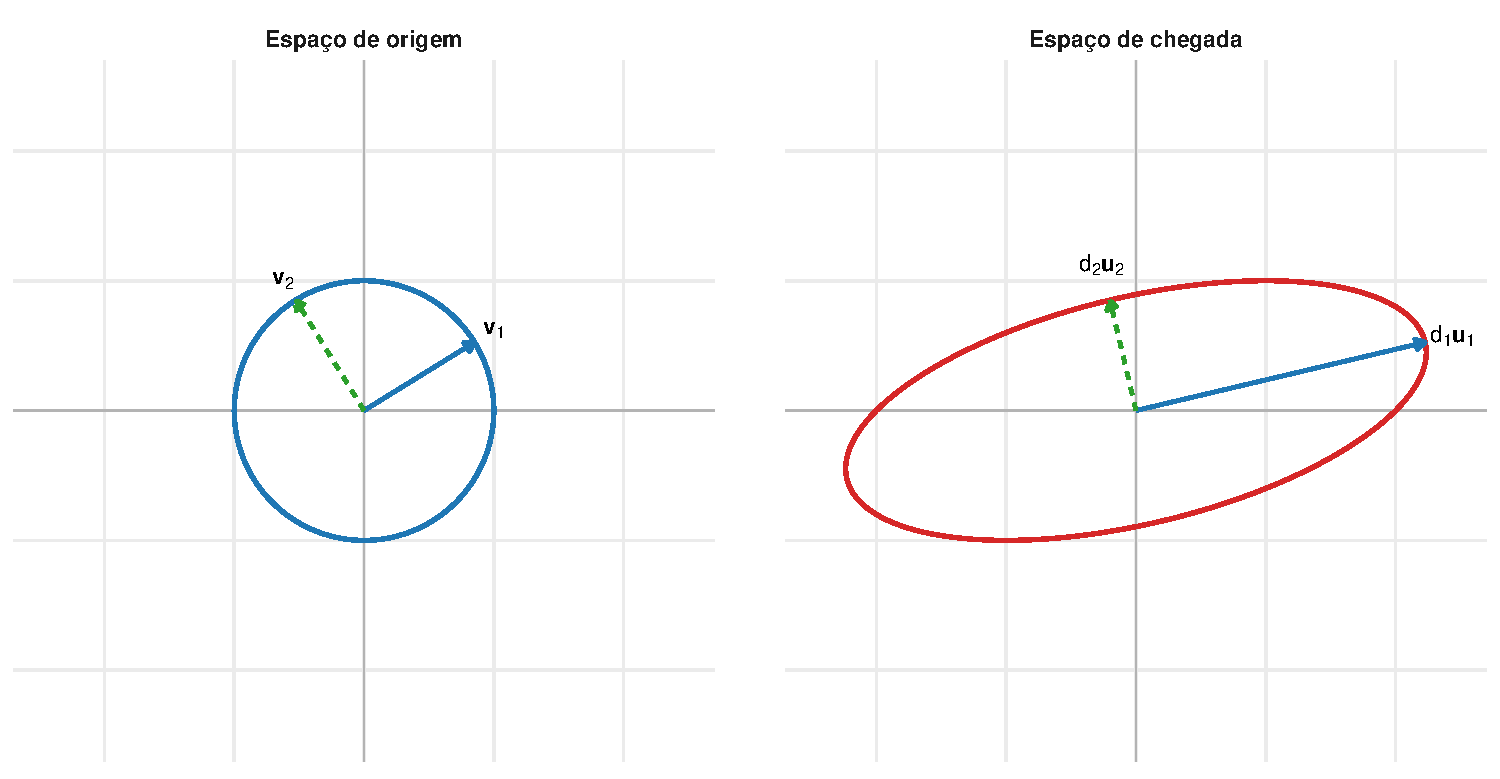
\includegraphics[keepaspectratio]{mod_1_svd_files/figure-pdf/fig-geometria-svd-1.pdf}}

}

\caption{\label{fig-geometria-svd}A SVD transforma as direções
singulares à direita nos semieixos da elipse orientados pelos vetores
singulares à esquerda.}

\end{figure}%

Neste exemplo, as bases singulares do domínio e do contradomínio são
distintas. A matriz \(\mathbf{V}^{\top}\) expressa os pontos da
circunferência nas coordenadas da base formada por \(\mathbf{v}_1\) e
\(\mathbf{v}_2\). Como essa transformação é ortogonal, a circunferência
permanece uma circunferência. Em seguida, \(\mathbf{D}\) realiza a
deformação, multiplicando os comprimentos nas duas direções por \(d_1\)
e \(d_2\). Finalmente, \(\mathbf{U}\) orienta os semieixos da elipse nas
direções \(\mathbf{u}_1\) e \(\mathbf{u}_2\) no espaço de chegada.

\subsection{Transformações com núcleo não
trivial}\label{transformauxe7uxf5es-com-nuxfacleo-nuxe3o-trivial}

Quando

\[
r<p,
\]

a transformação possui núcleo não trivial e elimina \(p-r\) direções
linearmente independentes do domínio. Geometricamente, a imagem da bola
unitária passa a ter dimensão inferior à dimensão do domínio.

\begin{example}[Colapso de uma direção pela
transformação]\protect\hypertarget{exm-nucleo-nao-trivial-svd}{}\label{exm-nucleo-nao-trivial-svd}

Considere

\[
\mathbf A_0
=
\begin{bmatrix}
2&0\\
0&0
\end{bmatrix}.
\]

Os valores singulares são

\[
d_1=2
\qquad
\text{e}
\qquad
d_2=0.
\]

A ação da transformação sobre um vetor

\[
\mathbf x
=
\begin{bmatrix}
x_1\\
x_2
\end{bmatrix}
\]

é

\[
\mathbf A_0\mathbf x
=
\begin{bmatrix}
2x_1\\
0
\end{bmatrix}.
\]

Portanto, toda a direção

\[
\mathbf e_2
=
\begin{bmatrix}
0\\
1
\end{bmatrix}
\]

é eliminada, pois

\[
\mathbf A_0\mathbf e_2
=
\mathbf 0.
\]

De fato,

\[
\mathcal N(\mathbf A_0)
=
\operatorname{span}
\left\{
\mathbf e_2
\right\}.
\]

A bola unitária de \(\mathbb R^2\) é transformada no segmento

\[
\left\{
\begin{bmatrix}
y_1\\
0
\end{bmatrix}
:
-2\leq y_1\leq2
\right\}.
\]

Assim, a imagem possui dimensão \(1\), que coincide com

\[
\operatorname{posto}(\mathbf A_0)=1.
\]

O valor singular positivo \(d_1=2\) determina o comprimento do único
semieixo não nulo, enquanto o valor singular \(d_2=0\) identifica a
direção eliminada pela transformação.

\end{example}

De modo geral:

\begin{itemize}
\tightlist
\item
  cada valor singular positivo produz um semieixo não nulo da imagem;
\item
  existem exatamente \(r\) semieixos não nulos;
\item
  o núcleo possui dimensão \(p-r\) e contém todas as direções que são
  transformadas no vetor nulo;
\item
  a dimensão do elipsoide resultante é \(r\);
\item
  o elipsoide está contido em \(\mathcal{C}(\mathbf{A})\).
\end{itemize}

A descrição geométrica da SVD também identifica bases ortonormais dos
quatro espaços fundamentais associados à matriz. Essas relações permitem
interpretar posto, núcleo, projetores e normas diretamente a partir dos
vetores e valores singulares. Aspectos relacionados ao condicionamento
numérico serão apresentados posteriormente como leitura de
aprofundamento.

\section{Espaços fundamentais, posto e
normas}\label{espauxe7os-fundamentais-posto-e-normas}

A SVD fornece bases ortonormais para os quatro espaços fundamentais
associados a uma matriz. Considere

\[
\mathbf{A}
\in
\mathbb{R}^{q\times p}
\]

com posto

\[
r
=
\operatorname{posto}(\mathbf{A})
\]

e SVD compacta

\[
\mathbf{A}
=
\mathbf{U}_r
\mathbf{D}_r
\mathbf{V}_r^{\top}.
\]

As colunas de

\[
\mathbf{U}_r
\in
\mathbb{R}^{q\times r}
\]

são os vetores singulares à esquerda associados aos valores singulares
positivos. As colunas de

\[
\mathbf{V}_r
\in
\mathbb{R}^{p\times r}
\]

são os vetores singulares à direita correspondentes.

Complete essas matrizes com bases ortonormais dos respectivos
complementos:

\[
\mathbf{U}
=
\begin{bmatrix}
\mathbf{U}_r&
\mathbf{U}_0
\end{bmatrix}
\]

e

\[
\mathbf{V}
=
\begin{bmatrix}
\mathbf{V}_r&
\mathbf{V}_0
\end{bmatrix},
\]

em que

\[
\mathbf{U}_0
\in
\mathbb{R}^{q\times(q-r)}
\]

e

\[
\mathbf{V}_0
\in
\mathbb{R}^{p\times(p-r)}.
\]

Quando \(r=q\), a matriz \(\mathbf{U}_0\) não possui colunas. Quando
\(r=p\), o mesmo ocorre com \(\mathbf{V}_0\).

\subsection{Espaço coluna e espaço
linha}\label{espauxe7o-coluna-e-espauxe7o-linha}

\begin{proposition}[Espaços fundamentais determinados pela
SVD]\protect\hypertarget{prp-espacos-fundamentais-svd}{}\label{prp-espacos-fundamentais-svd}

Se

\[
\mathbf{A}
=
\mathbf{U}_r
\mathbf{D}_r
\mathbf{V}_r^{\top}
\]

é a SVD compacta de uma matriz de posto \(r\), então

\[
\mathcal{C}(\mathbf{A})
=
\operatorname{span}
\left\{
\mathbf{u}_1,\ldots,\mathbf{u}_r
\right\}
=
\mathcal{C}(\mathbf{U}_r),
\]

\[
\mathcal{C}
\left(
\mathbf{A}^{\top}
\right)
=
\operatorname{span}
\left\{
\mathbf{v}_1,\ldots,\mathbf{v}_r
\right\}
=
\mathcal{C}(\mathbf{V}_r),
\]

\[
\mathcal{N}(\mathbf{A})
=
\operatorname{span}
\left\{
\mathbf{v}_{r+1},\ldots,\mathbf{v}_p
\right\}
=
\mathcal{C}(\mathbf{V}_0),
\]

e

\[
\mathcal{N}
\left(
\mathbf{A}^{\top}
\right)
=
\operatorname{span}
\left\{
\mathbf{u}_{r+1},\ldots,\mathbf{u}_q
\right\}
=
\mathcal{C}(\mathbf{U}_0).
\]

(Golub; Van Loan, 2013)

\end{proposition}

\begin{proof}
Pela SVD compacta,

\[
\mathbf{A}\mathbf{x}
=
\mathbf{U}_r
\mathbf{D}_r
\mathbf{V}_r^{\top}
\mathbf{x}
\]

para todo \(\mathbf{x}\in\mathbb{R}^{p}\). Logo, toda imagem de
\(\mathbf{A}\) é uma combinação linear das colunas de \(\mathbf{U}_r\):

\[
\mathcal{C}(\mathbf{A})
\subseteq
\mathcal{C}(\mathbf{U}_r).
\]

Reciprocamente, para cada \(j=1,\ldots,r\),

\[
\mathbf{A}\mathbf{v}_j
=
d_j\mathbf{u}_j.
\]

Como \(d_j>0\),

\[
\mathbf{u}_j
=
\mathbf{A}
\left(
\frac{1}{d_j}\mathbf{v}_j
\right).
\]

Portanto,

\[
\mathbf{u}_j
\in
\mathcal{C}(\mathbf{A}),
\]

e

\[
\mathcal{C}(\mathbf{U}_r)
\subseteq
\mathcal{C}(\mathbf{A}).
\]

Assim,

\[
\mathcal{C}(\mathbf{A})
=
\mathcal{C}(\mathbf{U}_r).
\]

Aplicando o mesmo argumento a

\[
\mathbf{A}^{\top}
=
\mathbf{V}_r
\mathbf{D}_r
\mathbf{U}_r^{\top},
\]

obtém-se

\[
\mathcal{C}
\left(
\mathbf{A}^{\top}
\right)
=
\mathcal{C}(\mathbf{V}_r).
\]

Considere agora a base ortonormal completa

\[
\mathbf{V}
=
\begin{bmatrix}
\mathbf{V}_r&
\mathbf{V}_0
\end{bmatrix}.
\]

Todo vetor \(\mathbf{x}\in\mathbb{R}^{p}\) possui uma decomposição única
da forma

\[
\mathbf{x}
=
\mathbf{V}_r\boldsymbol{\alpha}
+
\mathbf{V}_0\boldsymbol{\beta}.
\]

Aplicando \(\mathbf{A}\),

\[
\begin{aligned}
\mathbf{A}\mathbf{x}
&=
\mathbf{U}_r
\mathbf{D}_r
\mathbf{V}_r^{\top}
\left(
\mathbf{V}_r\boldsymbol{\alpha}
+
\mathbf{V}_0\boldsymbol{\beta}
\right)\\
&=
\mathbf{U}_r
\mathbf{D}_r
\boldsymbol{\alpha},
\end{aligned}
\]

pois

\[
\mathbf{V}_r^{\top}\mathbf{V}_r
=
\mathbf{I}_r
\]

e

\[
\mathbf{V}_r^{\top}\mathbf{V}_0
=
\mathbf{0}.
\]

Como \(\mathbf{D}_r\) é invertível,

\[
\mathbf{A}\mathbf{x}
=
\mathbf{0}
\]

se, e somente se,

\[
\boldsymbol{\alpha}
=
\mathbf{0}.
\]

Logo,

\[
\mathbf{x}
\in
\mathcal{N}(\mathbf{A})
\]

se, e somente se,

\[
\mathbf{x}
=
\mathbf{V}_0\boldsymbol{\beta}.
\]

Portanto,

\[
\mathcal{N}(\mathbf{A})
=
\mathcal{C}(\mathbf{V}_0).
\]

Aplicando o mesmo raciocínio a \(\mathbf{A}^{\top}\),

\[
\mathcal{N}
\left(
\mathbf{A}^{\top}
\right)
=
\mathcal{C}(\mathbf{U}_0).
\]

Assim, a SVD completa fornece bases ortonormais simultaneamente para os
quatro espaços fundamentais de \(\mathbf{A}\).
\end{proof}

As quatro bases fornecidas pela SVD podem ser organizadas como na
Tabela~\ref{tbl-espacos-svd}.

\begin{longtable}[]{@{}
  >{\raggedright\arraybackslash}p{(\linewidth - 6\tabcolsep) * \real{0.2500}}
  >{\raggedright\arraybackslash}p{(\linewidth - 6\tabcolsep) * \real{0.2500}}
  >{\raggedright\arraybackslash}p{(\linewidth - 6\tabcolsep) * \real{0.2500}}
  >{\raggedleft\arraybackslash}p{(\linewidth - 6\tabcolsep) * \real{0.2500}}@{}}
\caption{Espaços fundamentais e bases ortonormais fornecidas pela
SVD.}\label{tbl-espacos-svd}\tabularnewline
\toprule\noalign{}
\begin{minipage}[b]{\linewidth}\raggedright
Espaço
\end{minipage} & \begin{minipage}[b]{\linewidth}\raggedright
Subespaço de
\end{minipage} & \begin{minipage}[b]{\linewidth}\raggedright
Base ortonormal fornecida pela SVD
\end{minipage} & \begin{minipage}[b]{\linewidth}\raggedleft
Dimensão
\end{minipage} \\
\midrule\noalign{}
\endfirsthead
\toprule\noalign{}
\begin{minipage}[b]{\linewidth}\raggedright
Espaço
\end{minipage} & \begin{minipage}[b]{\linewidth}\raggedright
Subespaço de
\end{minipage} & \begin{minipage}[b]{\linewidth}\raggedright
Base ortonormal fornecida pela SVD
\end{minipage} & \begin{minipage}[b]{\linewidth}\raggedleft
Dimensão
\end{minipage} \\
\midrule\noalign{}
\endhead
\bottomrule\noalign{}
\endlastfoot
Espaço coluna \(\mathcal{C}(\mathbf{A})\) & \(\mathbb{R}^{q}\) & Colunas
de \(\mathbf{U}_r\) & \(r\) \\
Núcleo à esquerda \(\mathcal{N}(\mathbf{A}^{\top})\) &
\(\mathbb{R}^{q}\) & Colunas de \(\mathbf{U}_0\) & \(q-r\) \\
Espaço linha \(\mathcal{C}(\mathbf{A}^{\top})\) & \(\mathbb{R}^{p}\) &
Colunas de \(\mathbf{V}_r\) & \(r\) \\
Núcleo \(\mathcal{N}(\mathbf{A})\) & \(\mathbb{R}^{p}\) & Colunas de
\(\mathbf{V}_0\) & \(p-r\) \\
\end{longtable}

A SVD torna explícitas as decomposições ortogonais

\[
\mathbb{R}^{q}
=
\mathcal{C}(\mathbf{A})
\oplus
\mathcal{N}
\left(
\mathbf{A}^{\top}
\right)
\]

e

\[
\mathbb{R}^{p}
=
\mathcal{C}
\left(
\mathbf{A}^{\top}
\right)
\oplus
\mathcal{N}(\mathbf{A}).
\]

O símbolo \(\oplus\) indica uma soma direta ortogonal.

Todo vetor

\[
\mathbf{y}
\in
\mathbb{R}^{q}
\]

pode ser escrito de maneira única como

\[
\mathbf{y}
=
\mathbf{y}_{\mathcal{C}}
+
\mathbf{y}_{\mathcal{N}},
\]

com

\[
\mathbf{y}_{\mathcal{C}}
\in
\mathcal{C}(\mathbf{A})
\]

e

\[
\mathbf{y}_{\mathcal{N}}
\in
\mathcal{N}
\left(
\mathbf{A}^{\top}
\right).
\]

De modo análogo, todo vetor

\[
\mathbf{x}
\in
\mathbb{R}^{p}
\]

se decompõe em uma parcela no espaço linha e outra no núcleo de
\(\mathbf{A}\).

\subsection{Projetores ortogonais}\label{projetores-ortogonais}

A identificação das bases dos quatro espaços fundamentais permite
construir diretamente seus projetores ortogonais.

\begin{proposition}[Projetores dos espaços fundamentais pela
SVD]\protect\hypertarget{prp-projetores-espacos-svd}{}\label{prp-projetores-espacos-svd}

Considere a SVD completa escrita como

\[
\mathbf U
=
\begin{bmatrix}
\mathbf U_r&
\mathbf U_0
\end{bmatrix}
\]

e

\[
\mathbf V
=
\begin{bmatrix}
\mathbf V_r&
\mathbf V_0
\end{bmatrix}.
\]

Então, os projetores ortogonais sobre os quatro espaços fundamentais são

\[
\mathbf P_{\mathcal C(\mathbf A)}
=
\mathbf U_r
\mathbf U_r^{\top}
\]

e

\[
\mathbf P_{\mathcal N(\mathbf A^{\top})}
=
\mathbf U_0
\mathbf U_0^{\top}
=
\mathbf I_q
-
\mathbf U_r
\mathbf U_r^{\top}.
\]

No espaço de origem,

\[
\mathbf P_{\mathcal C(\mathbf A^{\top})}
=
\mathbf V_r
\mathbf V_r^{\top}
\]

e

\[
\mathbf P_{\mathcal N(\mathbf A)}
=
\mathbf V_0
\mathbf V_0^{\top}
=
\mathbf I_p
-
\mathbf V_r
\mathbf V_r^{\top}.
\]

\end{proposition}

\begin{proof}
Pela Proposição~\ref{prp-espacos-fundamentais-svd},

\[
\mathcal C(\mathbf A)
=
\mathcal C(\mathbf U_r)
\]

e

\[
\mathcal N(\mathbf A^{\top})
=
\mathcal C(\mathbf U_0).
\]

Como as colunas de \(\mathbf U_r\) e de \(\mathbf U_0\) são ortonormais,
a Proposição~\ref{prp-projecao-base-ortonormal} fornece

\[
\mathbf P_{\mathcal C(\mathbf A)}
=
\mathbf U_r
\mathbf U_r^{\top}
\]

e

\[
\mathbf P_{\mathcal N(\mathbf A^{\top})}
=
\mathbf U_0
\mathbf U_0^{\top}.
\]

Além disso, como

\[
\mathbf U
=
\begin{bmatrix}
\mathbf U_r&
\mathbf U_0
\end{bmatrix}
\]

é ortogonal,

\[
\mathbf U
\mathbf U^{\top}
=
\mathbf I_q.
\]

Portanto,

\[
\mathbf U_r
\mathbf U_r^{\top}
+
\mathbf U_0
\mathbf U_0^{\top}
=
\mathbf I_q,
\]

de onde

\[
\mathbf U_0
\mathbf U_0^{\top}
=
\mathbf I_q
-
\mathbf U_r
\mathbf U_r^{\top}.
\]

Aplicando o mesmo argumento a

\[
\mathbf V
=
\begin{bmatrix}
\mathbf V_r&
\mathbf V_0
\end{bmatrix},
\]

obtêm-se

\[
\mathbf P_{\mathcal C(\mathbf A^{\top})}
=
\mathbf V_r
\mathbf V_r^{\top}
\]

e

\[
\mathbf P_{\mathcal N(\mathbf A)}
=
\mathbf V_0
\mathbf V_0^{\top}
=
\mathbf I_p
-
\mathbf V_r
\mathbf V_r^{\top}.
\]
\end{proof}

Como são projetores ortogonais, essas matrizes são simétricas e
idempotentes, conforme as propriedades estudadas no Capítulo 3.

\begin{example}[Espaços fundamentais do exemplo
condutor]\protect\hypertarget{exm-espacos-fundamentais-svd}{}\label{exm-espacos-fundamentais-svd}

Considere novamente

\[
\mathbf{A}
=
\begin{bmatrix}
1&1\\
1&-1\\
1&1
\end{bmatrix}.
\]

Sua SVD completa foi construída com

\[
\mathbf{u}_1
=
\frac{1}{\sqrt{2}}
\begin{bmatrix}
1\\
0\\
1
\end{bmatrix},
\qquad
\mathbf{u}_2
=
\begin{bmatrix}
0\\
1\\
0
\end{bmatrix}
\]

e

\[
\mathbf{u}_3
=
\frac{1}{\sqrt{2}}
\begin{bmatrix}
1\\
0\\
-1
\end{bmatrix}.
\]

Os vetores singulares à direita são

\[
\mathbf{v}_1
=
\frac{1}{\sqrt{2}}
\begin{bmatrix}
1\\
1
\end{bmatrix}
\]

e

\[
\mathbf{v}_2
=
\frac{1}{\sqrt{2}}
\begin{bmatrix}
1\\
-1
\end{bmatrix}.
\]

Como os dois valores singulares são positivos,

\[
r=2.
\]

Assim,

\[
\mathcal{C}(\mathbf{A})
=
\operatorname{span}
\left\{
\mathbf{u}_1,\mathbf{u}_2
\right\},
\]

e

\[
\mathcal{N}
\left(
\mathbf{A}^{\top}
\right)
=
\operatorname{span}
\left\{
\mathbf{u}_3
\right\}.
\]

A matriz possui posto coluna completo, pois

\[
r=p=2.
\]

Consequentemente,

\[
\mathcal{N}(\mathbf{A})
=
\left\{
\mathbf{0}
\right\}
\]

e

\[
\mathcal{C}
\left(
\mathbf{A}^{\top}
\right)
=
\mathbb{R}^{2}.
\]

O projetor sobre o espaço coluna é

\[
\begin{aligned}
\mathbf{U}_2
\mathbf{U}_2^{\top}
&=
\mathbf{u}_1\mathbf{u}_1^{\top}
+
\mathbf{u}_2\mathbf{u}_2^{\top}\\
&=
\begin{bmatrix}
1/2&0&1/2\\
0&1&0\\
1/2&0&1/2
\end{bmatrix}.
\end{aligned}
\]

O projetor sobre o núcleo à esquerda é

\[
\begin{aligned}
\mathbf{u}_3\mathbf{u}_3^{\top}
&=
\begin{bmatrix}
1/2&0&-1/2\\
0&0&0\\
-1/2&0&1/2
\end{bmatrix}.
\end{aligned}
\]

A soma dos dois projetores é

\[
\mathbf{U}_2
\mathbf{U}_2^{\top}
+
\mathbf{u}_3
\mathbf{u}_3^{\top}
=
\mathbf{I}_3.
\]

\end{example}

\subsection{Posto e nulidades}\label{posto-e-nulidades}

Pela SVD, o posto de \(\mathbf A\) é exatamente o número de valores
singulares positivos:

\[
\operatorname{posto}(\mathbf A)
=
r
=
\#\left\{
j:
d_j>0
\right\}.
\]

Como consequência do Teorema Posto--Nulidade,

\[
\dim
\mathcal N(\mathbf A)
=
p-r
\]

e

\[
\dim
\mathcal N
\left(
\mathbf A^{\top}
\right)
=
q-r.
\]

Essas dimensões também são visualizadas diretamente na SVD completa:

\begin{itemize}
\tightlist
\item
  as \(r\) colunas de \(\mathbf V_r\) formam uma base do espaço linha;
\item
  as \(p-r\) colunas de \(\mathbf V_0\) formam uma base do núcleo de
  \(\mathbf A\);
\item
  as \(r\) colunas de \(\mathbf U_r\) formam uma base do espaço coluna;
\item
  as \(q-r\) colunas de \(\mathbf U_0\) formam uma base do núcleo de
  \(\mathbf A^{\top}\).
\end{itemize}

É importante distinguir essas dimensões do número de posições diagonais
nulas de \(\mathbf D\). Como

\[
\mathbf D
\in
\mathbb R^{q\times p}
\]

possui apenas

\[
s=\min(q,p)
\]

posições diagonais, existem

\[
s-r
\]

valores singulares nulos entre essas posições, enquanto as dimensões dos
dois núcleos são, respectivamente,

\[
p-r
\qquad\text{e}\qquad
q-r.
\]

Assim, em matrizes retangulares, a estrutura completa dos núcleos não
deve ser inferida apenas pela quantidade de elementos diagonais nulos de
\(\mathbf D\).

A Tabela~\ref{tbl-svd-estrutura-matriz} reúne as principais relações
entre os valores e vetores singulares e a estrutura da transformação.

\begin{longtable}[]{@{}
  >{\raggedright\arraybackslash}p{(\linewidth - 2\tabcolsep) * \real{0.5000}}
  >{\raggedright\arraybackslash}p{(\linewidth - 2\tabcolsep) * \real{0.5000}}@{}}
\caption{Relação entre a SVD e a estrutura da
matriz.}\label{tbl-svd-estrutura-matriz}\tabularnewline
\toprule\noalign{}
\begin{minipage}[b]{\linewidth}\raggedright
Estrutura ou propriedade
\end{minipage} & \begin{minipage}[b]{\linewidth}\raggedright
Caracterização pela SVD
\end{minipage} \\
\midrule\noalign{}
\endfirsthead
\toprule\noalign{}
\begin{minipage}[b]{\linewidth}\raggedright
Estrutura ou propriedade
\end{minipage} & \begin{minipage}[b]{\linewidth}\raggedright
Caracterização pela SVD
\end{minipage} \\
\midrule\noalign{}
\endhead
\bottomrule\noalign{}
\endlastfoot
Posto & Número de valores singulares positivos \\
Imagem \(\mathcal{C}(\mathbf{A})\) & Vetores singulares à esquerda
associados a \(d_j>0\) \\
Espaço linha \(\mathcal{C}(\mathbf{A}^{\top})\) & Vetores singulares à
direita associados a \(d_j>0\) \\
Núcleo \(\mathcal{N}(\mathbf{A})\) & Vetores singulares à direita
associados à parte nula \\
Núcleo à esquerda \(\mathcal{N}(\mathbf{A}^{\top})\) & Vetores
singulares à esquerda associados à parte nula \\
Ampliação máxima & \(d_1\) \\
Menor fator positivo de escala & \(d_r\) \\
\end{longtable}

Se \(r<p\), a menor norma de \(\mathbf{A}\mathbf{x}\) entre todos os
vetores unitários do domínio é zero, pois existem vetores unitários no
núcleo. O valor \(d_r\) descreve o menor fator \textbf{positivo} de
escala, isto é, a menor ação da transformação quando restrita ao espaço
linha \(\mathcal{C}(\mathbf{A}^{\top})\).

\subsection{Produto interno de
Frobenius}\label{produto-interno-de-frobenius}

O estudo das aproximações matriciais exige uma geometria para o espaço
das matrizes.

\begin{definition}[Produto interno de
Frobenius]\protect\hypertarget{def-produto-interno-frobenius}{}\label{def-produto-interno-frobenius}

Para matrizes

\[
\mathbf{A},
\widetilde{\mathbf{A}}
\in
\mathbb{R}^{q\times p},
\]

o \textbf{produto interno de Frobenius} é

\[
\left\langle
\mathbf{A},
\widetilde{\mathbf{A}}
\right\rangle_F
=
\operatorname{tr}
\left(
\mathbf{A}^{\top}
\widetilde{\mathbf{A}}
\right).
\]

Equivalentemente,

\[
\left\langle
\mathbf{A},
\widetilde{\mathbf{A}}
\right\rangle_F
=
\sum_{i=1}^{q}
\sum_{j=1}^{p}
a_{ij}\widetilde{a}_{ij}.
\]

\end{definition}

O produto interno de Frobenius trata uma matriz como um vetor formado
por todos os seus elementos. Duas matrizes são ortogonais segundo esse
produto quando

\[
\left\langle
\mathbf{A},
\widetilde{\mathbf{A}}
\right\rangle_F
=
0.
\]

A norma induzida por esse produto interno é a norma de Frobenius.

\begin{definition}[Norma de
Frobenius]\protect\hypertarget{def-norma-frobenius}{}\label{def-norma-frobenius}

A \textbf{norma de Frobenius} de

\[
\mathbf{A}
=
(a_{ij})
\in
\mathbb{R}^{q\times p}
\]

é

\[
\|\mathbf{A}\|_F
=
\sqrt{
\left\langle
\mathbf{A},
\mathbf{A}
\right\rangle_F
}.
\]

Equivalentemente,

\[
\|\mathbf{A}\|_F
=
\sqrt{
\operatorname{tr}
\left(
\mathbf{A}^{\top}\mathbf{A}
\right)
}
\]

ou

\[
\|\mathbf{A}\|_F
=
\sqrt{
\sum_{i=1}^{q}
\sum_{j=1}^{p}
a_{ij}^2
}.
\]

\end{definition}

A norma de Frobenius mede a magnitude quadrática total dos elementos da
matriz.

\subsection{Normas e valores
singulares}\label{normas-e-valores-singulares}

\begin{definition}[Norma
espectral]\protect\hypertarget{def-norma-espectral}{}\label{def-norma-espectral}

A \textbf{norma espectral}, ou norma matricial induzida pela norma
euclidiana, é

\[
\|\mathbf{A}\|_2
=
\max_{\mathbf{x}\neq\mathbf{0}}
\frac{
\|\mathbf{A}\mathbf{x}\|
}{
\|\mathbf{x}\|
}.
\]

Equivalentemente,

\[
\|\mathbf{A}\|_2
=
\max_{\|\mathbf{x}\|=1}
\|\mathbf{A}\mathbf{x}\|.
\]

\end{definition}

A interpretação geométrica anterior mostra que a norma espectral é o
maior fator de ampliação produzido pela transformação.

\begin{proposition}[Normas matriciais e valores
singulares]\protect\hypertarget{prp-normas-valores-singulares}{}\label{prp-normas-valores-singulares}

Se

\[
d_1
\geq
\cdots
\geq
d_r
>
0
\]

são os valores singulares positivos de \(\mathbf{A}\), então

\[
\|\mathbf{A}\|_2
=
d_1
\]

e

\[
\|\mathbf{A}\|_F^2
=
\sum_{j=1}^{r}d_j^2.
\]

(Golub; Van Loan, 2013)

\end{proposition}

\begin{proof}
Pela Proposição~\ref{prp-extremos-comprimentos-svd},

\[
\max_{\|\mathbf x\|=1}
\|\mathbf A\mathbf x\|
=
d_1.
\]

Como, pela Definição~\ref{def-norma-espectral},

\[
\|\mathbf A\|_2
=
\max_{\|\mathbf x\|=1}
\|\mathbf A\mathbf x\|,
\]

segue imediatamente que

\[
\|\mathbf A\|_2
=
d_1.
\]

Para a norma de Frobenius, utilizando a
Proposição~\ref{prp-decomposicoes-espectrais-svd},

\[
\mathbf A^{\top}\mathbf A
=
\mathbf V_r
\mathbf D_r^2
\mathbf V_r^{\top}.
\]

Portanto,

\[
\begin{aligned}
\|\mathbf A\|_F^2
&=
\operatorname{tr}
\left(
\mathbf A^{\top}\mathbf A
\right)\\
&=
\operatorname{tr}
\left(
\mathbf V_r
\mathbf D_r^2
\mathbf V_r^{\top}
\right)\\
&=
\operatorname{tr}
\left(
\mathbf D_r^2
\mathbf V_r^{\top}
\mathbf V_r
\right)\\
&=
\operatorname{tr}
\left(
\mathbf D_r^2
\right)\\
&=
\sum_{j=1}^{r}
d_j^2.
\end{aligned}
\]

Logo,

\[
\|\mathbf A\|_F^2
=
\sum_{j=1}^{r}
d_j^2.
\]
\end{proof}

Se \(\mathbf{A}=\mathbf{0}\), então não há valores singulares positivos
e, diretamente pelas definições,

\[
\|\mathbf{A}\|_2
=
\|\mathbf{A}\|_F
=
0.
\]

As duas normas medem aspectos diferentes:

\begin{itemize}
\tightlist
\item
  \(\|\mathbf{A}\|_2\) depende somente do maior valor singular e
  representa o maior fator de ampliação;
\item
  \(\|\mathbf{A}\|_F\) reúne as contribuições quadráticas de todos os
  valores singulares.
\end{itemize}

Para qualquer matriz,

\[
\|\mathbf{A}\|_2
\leq
\|\mathbf{A}\|_F
\leq
\sqrt{r}
\|\mathbf{A}\|_2.
\]

A primeira desigualdade decorre de

\[
d_1^2
\leq
\sum_{j=1}^{r}d_j^2.
\]

A segunda decorre de

\[
\sum_{j=1}^{r}d_j^2
\leq
r d_1^2.
\]

\subsection{Invariância ortogonal}\label{invariuxe2ncia-ortogonal}

As normas espectral e de Frobenius são preservadas por multiplicações
ortogonais.

\begin{proposition}[Invariância ortogonal das
normas]\protect\hypertarget{prp-invariancia-ortogonal-normas}{}\label{prp-invariancia-ortogonal-normas}

Se \(\mathbf{Q}_1\) e \(\mathbf{Q}_2\) são matrizes ortogonais de
dimensões compatíveis, então

\[
\left\|
\mathbf{Q}_1
\mathbf{A}
\mathbf{Q}_2
\right\|_2
=
\|\mathbf{A}\|_2
\]

e

\[
\left\|
\mathbf{Q}_1
\mathbf{A}
\mathbf{Q}_2
\right\|_F
=
\|\mathbf{A}\|_F.
\]

(Golub; Van Loan, 2013)

\end{proposition}

\begin{proof}
Para a norma espectral, como \(\mathbf{Q}_1\) preserva normas,

\[
\left\|
\mathbf{Q}_1
\mathbf{A}
\mathbf{Q}_2
\mathbf{x}
\right\|
=
\left\|
\mathbf{A}
\mathbf{Q}_2
\mathbf{x}
\right\|.
\]

Como \(\mathbf{Q}_2\) é ortogonal, a transformação

\[
\mathbf{z}
=
\mathbf{Q}_2\mathbf{x}
\]

preserva a norma e percorre todos os vetores unitários quando
\(\mathbf{x}\) percorre a esfera unitária. Portanto,

\[
\begin{aligned}
\left\|
\mathbf{Q}_1
\mathbf{A}
\mathbf{Q}_2
\right\|_2
&=
\max_{\|\mathbf{x}\|=1}
\left\|
\mathbf{A}
\mathbf{Q}_2
\mathbf{x}
\right\|\\
&=
\max_{\|\mathbf{z}\|=1}
\|\mathbf{A}\mathbf{z}\|\\
&=
\|\mathbf{A}\|_2.
\end{aligned}
\]

Para a norma de Frobenius,

\[
\begin{aligned}
\left\|
\mathbf{Q}_1
\mathbf{A}
\mathbf{Q}_2
\right\|_F^2
&=
\operatorname{tr}
\left[
\left(
\mathbf{Q}_1
\mathbf{A}
\mathbf{Q}_2
\right)^{\top}
\left(
\mathbf{Q}_1
\mathbf{A}
\mathbf{Q}_2
\right)
\right]\\
&=
\operatorname{tr}
\left(
\mathbf{Q}_2^{\top}
\mathbf{A}^{\top}
\mathbf{A}
\mathbf{Q}_2
\right)\\
&=
\operatorname{tr}
\left(
\mathbf{A}^{\top}
\mathbf{A}
\mathbf{Q}_2
\mathbf{Q}_2^{\top}
\right)\\
&=
\operatorname{tr}
\left(
\mathbf{A}^{\top}
\mathbf{A}
\right)\\
&=
\|\mathbf{A}\|_F^2.
\end{aligned}
\]

Logo, ambas as normas são invariantes sob multiplicações ortogonais.
\end{proof}

A SVD pode, portanto, ser interpretada como uma representação que remove
fatores ortogonais sem alterar essas normas:

\[
\|\mathbf{A}\|_2
=
\|\mathbf{D}\|_2
\]

e

\[
\|\mathbf{A}\|_F
=
\|\mathbf{D}\|_F.
\]

\subsection{Determinante e
invertibilidade}\label{determinante-e-invertibilidade-1}

Quando

\[
q=p,
\]

a matriz \(\mathbf{A}\) é quadrada. Pela SVD,

\[
\det(\mathbf{A})
=
\det(\mathbf{U})
\det(\mathbf{D})
\det
\left(
\mathbf{V}^{\top}
\right).
\]

Como \(\mathbf{U}\) e \(\mathbf{V}\) são ortogonais,

\[
\left|
\det(\mathbf{U})
\right|
=
\left|
\det(\mathbf{V})
\right|
=
1.
\]

Portanto,

\[
\left|
\det(\mathbf{A})
\right|
=
\prod_{j=1}^{p}d_j.
\]

O módulo do determinante é o produto dos valores singulares.

Além disso,

\[
\mathbf{A}
\text{ é invertível}
\iff
d_j>0
\quad
\text{para todo }j.
\]

Nesse caso,

\[
r=p=q,
\]

de modo que não existem direções singulares associadas ao valor zero.
Assim, as formas compacta e completa possuem as mesmas dimensões e podem
ser escritas com os mesmos fatores:

\[
\mathbf U_r=\mathbf U,
\qquad
\mathbf D_r=\mathbf D,
\qquad
\mathbf V_r=\mathbf V.
\]

\subsection{Aprofundamento: condicionamento e posto
numérico}\label{aprofundamento-condicionamento-e-posto-numuxe9rico}

\begin{tcolorbox}[enhanced jigsaw, colback=white, breakable, bottomrule=.15mm, left=2mm, arc=.35mm, rightrule=.15mm, colframe=quarto-callout-note-color-frame, toprule=.15mm, leftrule=.75mm, opacityback=0]

\vspace{-3mm}\textbf{Leitura de aprofundamento}\vspace{3mm}

Esta seção apresenta duas extensões de natureza numérica da
interpretação dos valores singulares. A primeira utiliza a razão entre
os valores singulares extremos para avaliar o condicionamento de uma
transformação. A segunda distingue o posto algébrico do posto numérico
obtido após a adoção de uma tolerância computacional.

Esses conceitos são importantes para estabilidade numérica, problemas
inversos e algoritmos matriciais, mas não são necessários para
acompanhar os resultados centrais sobre espaços fundamentais,
aproximações de posto reduzido e aplicações estatísticas da SVD.

\end{tcolorbox}

Considere

\[
\mathbf A
\in
\mathbb R^{q\times p}
\]

e defina

\[
s
=
\min(q,p).
\]

Quando

\[
\operatorname{posto}(\mathbf A)=s,
\]

a matriz possui o maior posto possível para suas dimensões e todos os
seus \(s\) valores singulares são positivos:

\[
d_1
\geq
\cdots
\geq
d_s
>
0.
\]

\begin{definition}[Número de condição na norma
espectral]\protect\hypertarget{def-numero-condicao-svd}{}\label{def-numero-condicao-svd}

Para uma matriz de posto máximo,

\[
\operatorname{posto}(\mathbf A)=s,
\]

define-se o \textbf{número de condição na norma espectral} por

\[
\kappa_2(\mathbf A)
=
\frac{d_1}{d_s}.
\]

Quando

\[
\operatorname{posto}(\mathbf A)<s,
\]

adota-se

\[
\kappa_2(\mathbf A)
=
\infty.
\]

(Golub; Van Loan, 2013)

\end{definition}

O número de condição compara o maior e o menor fatores positivos de
escala associados à parte ativa da transformação.

Quando

\[
\kappa_2(\mathbf A)
\approx
1,
\]

os valores singulares extremos possuem magnitudes semelhantes. Quando

\[
\kappa_2(\mathbf A)
\]

é elevado, algumas direções ativas são transformadas por fatores muito
maiores que outras.

É importante distinguir \textbf{núcleo não trivial}, \textbf{deficiência
de posto} e \textbf{mau condicionamento}.

A deficiência de posto ocorre quando

\[
\operatorname{posto}(\mathbf A)
<
\min(q,p).
\]

Entretanto, uma matriz retangular pode possuir núcleo não trivial mesmo
apresentando posto máximo.

Por exemplo, se

\[
q<p
\]

e

\[
\operatorname{posto}(\mathbf A)=q,
\]

então \(\mathbf A\) possui posto linha completo e, portanto, posto
máximo. Mesmo assim,

\[
\dim
\mathcal N(\mathbf A)
=
p-q
>
0.
\]

Assim, existem direções do domínio que são transformadas no vetor nulo.

Nesse caso, a transformação não é injetiva em todo o domínio
\(\mathbb R^p\). Sua restrição ao espaço linha,

\[
\mathcal C
\left(
\mathbf A^{\top}
\right)
=
\mathcal N(\mathbf A)^{\perp},
\]

é, entretanto, injetiva.

Nesse subespaço,

\[
d_q
=
\min_{
\substack{
\|\mathbf x\|=1\\
\mathbf x\in
\mathcal C(\mathbf A^{\top})
}
}
\|\mathbf A\mathbf x\|.
\]

Portanto, para matrizes largas de posto linha completo, o número de
condição finito descreve a variação dos fatores de escala sobre o espaço
linha, isto é, sobre a parte do domínio na qual a transformação atua de
forma injetiva.

Se

\[
q\geq p
\]

e

\[
\operatorname{posto}(\mathbf A)=p,
\]

então \(\mathbf A\) possui posto coluna completo e

\[
\mathcal N(\mathbf A)
=
\{\mathbf0\}.
\]

Nesse caso,

\[
d_p
=
\min_{\|\mathbf x\|=1}
\|\mathbf A\mathbf x\|
\]

e

\[
\kappa_2(\mathbf A)
=
\frac{d_1}{d_p}.
\]

Para uma matriz quadrada invertível,

\[
q=p=r,
\]

tem-se também

\[
\kappa_2(\mathbf A)
=
\|\mathbf A\|_2
\left\|
\mathbf A^{-1}
\right\|_2.
\]

De fato,

\[
\|\mathbf A\|_2
=
d_1,
\]

e os valores singulares de \(\mathbf A^{-1}\) são

\[
\frac{1}{d_p},
\ldots,
\frac{1}{d_1}.
\]

Portanto,

\[
\left\|
\mathbf A^{-1}
\right\|_2
=
\frac{1}{d_p},
\]

de modo que

\[
\kappa_2(\mathbf A)
=
\frac{d_1}{d_p}.
\]

Uma matriz de posto máximo com número de condição elevado é denominada
\textbf{mal condicionada}. Valores singulares positivos muito pequenos
indicam direções nas quais a transformação produz forte contração. Ao
inverter a ação da matriz nessas direções, pequenas perturbações podem
ser amplificadas.

Esse fenômeno será retomado posteriormente na discussão da
pseudoinversa.

\begin{example}[Comparação entre duas
transformações]\protect\hypertarget{exm-condicionamento-svd}{}\label{exm-condicionamento-svd}

Considere

\[
\mathbf A_1
=
\begin{bmatrix}
2&0\\
0&2
\end{bmatrix}
\]

e

\[
\mathbf A_2
=
\begin{bmatrix}
2&0\\
0&0{,}02
\end{bmatrix}.
\]

Os valores singulares de \(\mathbf A_1\) são

\[
2
\qquad
\text{e}
\qquad
2.
\]

Portanto,

\[
\kappa_2(\mathbf A_1)
=
1.
\]

Nesse caso, as duas direções singulares são transformadas pelo mesmo
fator.

Para \(\mathbf A_2\), os valores singulares são

\[
2
\qquad
\text{e}
\qquad
0{,}02.
\]

Logo,

\[
\kappa_2(\mathbf A_2)
=
\frac{2}{0{,}02}
=
100.
\]

A primeira direção é ampliada por um fator igual a \(2\), enquanto a
segunda é contraída por um fator igual a \(0{,}02\).

A inversão da segunda componente exige um fator

\[
\frac{1}{0{,}02}
=
50.
\]

Consequentemente, pequenas perturbações nessa direção podem ser
fortemente ampliadas quando se procura inverter a transformação.

\end{example}

\subsubsection{Posto exato e posto
numérico}\label{posto-exato-e-posto-numuxe9rico}

Matematicamente, o posto é determinado exatamente pelos valores
singulares positivos:

\[
\operatorname{posto}(\mathbf A)
=
\#\left\{
j:
d_j>0
\right\}.
\]

Em cálculos computacionais, entretanto, valores que seriam exatamente
nulos em aritmética exata podem aparecer como números positivos muito
pequenos em razão de arredondamentos, aproximações ou ruído.

Por isso, pode-se adotar uma tolerância

\[
\tau\geq0
\]

e tratar como numericamente nulos os valores singulares que satisfazem

\[
d_j
\leq
\tau.
\]

\begin{definition}[Posto
numérico]\protect\hypertarget{def-posto-numerico}{}\label{def-posto-numerico}

Fixada uma tolerância \(\tau\geq0\), o \textbf{posto numérico} de
\(\mathbf A\) é definido por

\[
r_{\tau}(\mathbf A)
=
\#\left\{
j:
d_j>\tau
\right\}.
\]

\end{definition}

Diferentemente do posto algébrico, o posto numérico depende da
tolerância adotada.

A escolha de \(\tau\) pode depender de fatores como:

\begin{itemize}
\tightlist
\item
  precisão numérica;
\item
  escala da matriz;
\item
  dimensões da matriz;
\item
  finalidade da análise;
\item
  nível de perturbação ou ruído considerado relevante.
\end{itemize}

Portanto, dois valores devem ser distinguidos:

\[
\operatorname{posto}(\mathbf A)
=
\#\{j:d_j>0\}
\]

e

\[
r_{\tau}(\mathbf A)
=
\#\{j:d_j>\tau\}.
\]

Essa distinção será particularmente útil quando forem estudadas
aproximações de posto reduzido. Nessas aproximações, valores singulares
matematicamente positivos podem ser descartados deliberadamente quando
sua contribuição é considerada pequena.

\section{SVD de uma matriz de dados}\label{svd-de-uma-matriz-de-dados}

Considere uma matriz de dados

\[
\mathbf{X}
\in
\mathbb{R}^{n\times p},
\]

em que as linhas representam \(n\) observações e as colunas representam
\(p\) variáveis.

Se

\[
r
=
\operatorname{posto}(\mathbf{X}),
\]

a SVD compacta é

\[
\mathbf{X}
=
\mathbf{U}_r
\mathbf{D}_r
\mathbf{V}_r^{\top},
\]

com

\[
\mathbf{U}_r
\in
\mathbb{R}^{n\times r},
\qquad
\mathbf{D}_r
\in
\mathbb{R}^{r\times r}
\]

e

\[
\mathbf{V}_r
\in
\mathbb{R}^{p\times r}.
\]

Nesse contexto, a SVD recupera a dupla representação da matriz de dados
introduzida no Capítulo 1:

\begin{itemize}
\tightlist
\item
  as colunas de \(\mathbf{V}_r\) pertencem a \(\mathbb{R}^{p}\) e
  determinam direções no espaço em que as observações são representadas;
\item
  as colunas de \(\mathbf{U}_r\) pertencem a \(\mathbb{R}^{n}\) e
  determinam direções no espaço em que as variáveis são representadas.
\end{itemize}

Os mesmos valores singulares conectam essas duas representações.

\subsection{Dualidade entre observações e
variáveis}\label{dualidade-entre-observauxe7uxf5es-e-variuxe1veis}

A SVD relaciona diretamente as duas representações da matriz de dados:
as observações como vetores em \(\mathbb R^p\) e as variáveis como
vetores em \(\mathbb R^n\).

\begin{proposition}[Dualidade entre observações e
variáveis]\protect\hypertarget{prp-dualidade-svd-dados}{}\label{prp-dualidade-svd-dados}

Se

\[
\mathbf X
=
\mathbf U_r
\mathbf D_r
\mathbf V_r^{\top}
\]

é a SVD compacta de uma matriz de dados

\[
\mathbf X
\in
\mathbb R^{n\times p},
\]

então

\[
\mathbf X\mathbf V_r
=
\mathbf U_r\mathbf D_r
\]

e

\[
\mathbf X^{\top}\mathbf U_r
=
\mathbf V_r\mathbf D_r.
\]

Consequentemente, para

\[
j=1,\ldots,r,
\]

tem-se

\[
\mathbf X\mathbf v_j
=
d_j\mathbf u_j
\]

e

\[
\mathbf X^{\top}\mathbf u_j
=
d_j\mathbf v_j.
\]

Assim, o mesmo valor singular \(d_j\) relaciona uma direção
\(\mathbf v_j\) no espaço das observações \(\mathbb R^p\) a uma direção
\(\mathbf u_j\) no espaço das variáveis \(\mathbb R^n\).

\end{proposition}

\begin{proof}
Multiplicando a SVD compacta à direita por \(\mathbf V_r\),

\[
\begin{aligned}
\mathbf X\mathbf V_r
&=
\mathbf U_r
\mathbf D_r
\mathbf V_r^{\top}
\mathbf V_r\\
&=
\mathbf U_r
\mathbf D_r,
\end{aligned}
\]

pois

\[
\mathbf V_r^{\top}\mathbf V_r
=
\mathbf I_r.
\]

Transpondo a SVD compacta,

\[
\mathbf X^{\top}
=
\mathbf V_r
\mathbf D_r
\mathbf U_r^{\top}.
\]

Multiplicando à direita por \(\mathbf U_r\),

\[
\begin{aligned}
\mathbf X^{\top}\mathbf U_r
&=
\mathbf V_r
\mathbf D_r
\mathbf U_r^{\top}
\mathbf U_r\\
&=
\mathbf V_r
\mathbf D_r,
\end{aligned}
\]

pois

\[
\mathbf U_r^{\top}\mathbf U_r
=
\mathbf I_r.
\]

As relações correspondentes a cada coluna seguem diretamente dessas duas
identidades matriciais.
\end{proof}

\subsection{Coordenadas das observações nas direções singulares à
direita}\label{coordenadas-das-observauxe7uxf5es-nas-direuxe7uxf5es-singulares-uxe0-direita}

Defina

\[
\mathbf Z
=
\mathbf X\mathbf V_r.
\]

Pela Proposição~\ref{prp-dualidade-svd-dados},

\[
\mathbf Z
=
\mathbf U_r\mathbf D_r.
\]

A matriz

\[
\mathbf Z
\in
\mathbb R^{n\times r}
\]

contém as coordenadas das observações na base ortonormal

\[
\left\{
\mathbf v_1,\ldots,\mathbf v_r
\right\}
\]

do espaço linha

\[
\mathcal C
\left(
\mathbf X^{\top}
\right)
\subseteq
\mathbb R^p.
\]

Como cada observação pertence a esse subespaço, as \(r\) coordenadas são
suficientes para representá-la exatamente.

Se a linha \(i\) de \(\mathbf X\) corresponde ao vetor

\[
\mathbf x_i
\in
\mathbb R^p,
\]

então

\[
z_{ij}
=
\mathbf x_i^{\top}\mathbf v_j.
\]

Portanto, \(z_{ij}\) é a coordenada da observação \(i\) na direção
singular \(\mathbf v_j\).

A \(j\)-ésima coluna de \(\mathbf Z\) é

\[
\mathbf z_j
=
\mathbf X\mathbf v_j
=
d_j\mathbf u_j.
\]

Assim, \(\mathbf v_j\) determina a direção utilizada para representar as
observações, enquanto \(\mathbf u_j\) descreve como as coordenadas
correspondentes se distribuem entre as \(n\) unidades observacionais.

\subsection{Coordenadas das variáveis nas direções singulares à
esquerda}\label{coordenadas-das-variuxe1veis-nas-direuxe7uxf5es-singulares-uxe0-esquerda}

A relação dual é

\[
\mathbf U_r^{\top}\mathbf X
=
\mathbf D_r\mathbf V_r^{\top}.
\]

Defina

\[
\mathbf W
=
\mathbf U_r^{\top}\mathbf X
\in
\mathbb R^{r\times p}.
\]

Cada coluna de \(\mathbf X\) representa uma variável como vetor em
\(\mathbb R^n\). Se

\[
\mathbf x^{(j)}
\in
\mathbb R^n
\]

denota a \(j\)-ésima variável, então a \(j\)-ésima coluna de
\(\mathbf W\) contém suas coordenadas na base ortonormal

\[
\left\{
\mathbf u_1,\ldots,\mathbf u_r
\right\}
\]

do espaço coluna

\[
\mathcal C(\mathbf X)
\subseteq
\mathbb R^n.
\]

Para a direção singular \(\ell\),

\[
\mathbf u_{\ell}^{\top}
\mathbf x^{(j)}
=
d_{\ell}v_{j\ell}.
\]

Portanto, os elementos de \(\mathbf V_r\), escalonados pelos valores
singulares, também descrevem as coordenadas das variáveis na base
singular à esquerda.

As relações

\[
\mathbf X\mathbf V_r
=
\mathbf U_r\mathbf D_r
\]

e

\[
\mathbf X^{\top}\mathbf U_r
=
\mathbf V_r\mathbf D_r
\]

expressam, assim, a dualidade entre o espaço das observações e o espaço
das variáveis.

\subsection{Matrizes de Gram da matriz de
dados}\label{matrizes-de-gram-da-matriz-de-dados}

As duas matrizes de Gram associadas a \(\mathbf X\) descrevem relações
entre objetos diferentes.

A matriz

\[
\mathbf X^{\top}\mathbf X
\in
\mathbb R^{p\times p}
\]

reúne os produtos internos entre as colunas de \(\mathbf X\), isto é,
entre as variáveis representadas como vetores em \(\mathbb R^n\).

A matriz

\[
\mathbf X\mathbf X^{\top}
\in
\mathbb R^{n\times n}
\]

reúne os produtos internos entre as linhas de \(\mathbf X\), isto é,
entre as observações representadas como vetores em \(\mathbb R^p\).

Pela Proposição~\ref{prp-decomposicoes-espectrais-svd},

\[
\mathbf X^{\top}\mathbf X
=
\mathbf V_r
\mathbf D_r^2
\mathbf V_r^{\top}
\]

e

\[
\mathbf X\mathbf X^{\top}
=
\mathbf U_r
\mathbf D_r^2
\mathbf U_r^{\top}.
\]

Portanto, as duas matrizes possuem os mesmos autovalores positivos,

\[
d_1^2,\ldots,d_r^2,
\]

mas seus autovetores pertencem a espaços diferentes:

\begin{itemize}
\tightlist
\item
  \(\mathbf v_j\in\mathbb R^p\) determina uma direção no espaço das
  observações;
\item
  \(\mathbf u_j\in\mathbb R^n\) determina uma direção no espaço das
  variáveis.
\end{itemize}

Essa dualidade também pode ser útil quando as dimensões da matriz são
muito diferentes. Se

\[
n\gg p,
\]

a matriz

\[
\mathbf X^{\top}\mathbf X
\]

possui ordem menor. Se

\[
p\gg n,
\]

a matriz

\[
\mathbf X\mathbf X^{\top}
\]

possui ordem menor.

Em ambos os casos, os valores próprios positivos são os mesmos e
correspondem aos quadrados dos valores singulares de \(\mathbf X\).

\subsection{Representação exata das
observações}\label{representauxe7uxe3o-exata-das-observauxe7uxf5es}

\begin{proposition}[Preservação da geometria pelas coordenadas
singulares]\protect\hypertarget{prp-geometria-coordenadas-singulares}{}\label{prp-geometria-coordenadas-singulares}

Seja

\[
\mathbf X
=
\mathbf U_r
\mathbf D_r
\mathbf V_r^{\top}
\]

a SVD compacta de uma matriz de dados e defina

\[
\mathbf Z
=
\mathbf X\mathbf V_r
=
\mathbf U_r\mathbf D_r.
\]

Então,

\[
\mathbf X
=
\mathbf Z\mathbf V_r^{\top}
\]

e

\[
\mathbf Z\mathbf Z^{\top}
=
\mathbf X\mathbf X^{\top}.
\]

Consequentemente, para quaisquer observações \(\mathbf x_i\) e
\(\mathbf x_{\ell}\), com coordenadas correspondentes \(\mathbf z_i\) e
\(\mathbf z_{\ell}\),

\[
\mathbf x_i^{\top}\mathbf x_{\ell}
=
\mathbf z_i^{\top}\mathbf z_{\ell},
\]

\[
\|\mathbf x_i\|
=
\|\mathbf z_i\|
\]

e

\[
\|\mathbf x_i-\mathbf x_{\ell}\|
=
\|\mathbf z_i-\mathbf z_{\ell}\|.
\]

\end{proposition}

\begin{proof}
Como

\[
\mathbf Z
=
\mathbf U_r\mathbf D_r,
\]

segue da SVD compacta que

\[
\mathbf X
=
\mathbf U_r
\mathbf D_r
\mathbf V_r^{\top}
=
\mathbf Z
\mathbf V_r^{\top}.
\]

Além disso,

\[
\begin{aligned}
\mathbf Z\mathbf Z^{\top}
&=
\mathbf U_r
\mathbf D_r
\mathbf D_r
\mathbf U_r^{\top}\\
&=
\mathbf U_r
\mathbf D_r^2
\mathbf U_r^{\top}.
\end{aligned}
\]

Pela Proposição~\ref{prp-decomposicoes-espectrais-svd},

\[
\mathbf X\mathbf X^{\top}
=
\mathbf U_r
\mathbf D_r^2
\mathbf U_r^{\top}.
\]

Portanto,

\[
\mathbf Z\mathbf Z^{\top}
=
\mathbf X\mathbf X^{\top}.
\]

Os elementos dessas duas matrizes são os produtos internos entre pares
de observações. Logo,

\[
\mathbf x_i^{\top}\mathbf x_{\ell}
=
\mathbf z_i^{\top}\mathbf z_{\ell}.
\]

Tomando \(i=\ell\), obtém-se

\[
\|\mathbf x_i\|^2
=
\|\mathbf z_i\|^2.
\]

Finalmente,

\[
\begin{aligned}
\|\mathbf x_i-\mathbf x_{\ell}\|^2
&=
\|\mathbf x_i\|^2
+
\|\mathbf x_{\ell}\|^2
-
2\mathbf x_i^{\top}\mathbf x_{\ell}\\
&=
\|\mathbf z_i\|^2
+
\|\mathbf z_{\ell}\|^2
-
2\mathbf z_i^{\top}\mathbf z_{\ell}\\
&=
\|\mathbf z_i-\mathbf z_{\ell}\|^2.
\end{aligned}
\]
\end{proof}

A reconstrução de cada observação pode ser escrita como

\[
\mathbf x_i
=
\sum_{j=1}^{r}
z_{ij}\mathbf v_j.
\]

Portanto,

\[
\mathbf x_i
\in
\mathcal C(\mathbf V_r)
\subseteq
\mathbb R^p.
\]

Se

\[
r<p,
\]

as observações podem ser representadas exatamente por apenas \(r\)
coordenadas, sem alteração de seus produtos internos, normas ou
distâncias euclidianas.

Essa situação pode ocorrer mesmo quando \(\mathbf X\) possui o maior
posto possível para suas dimensões. Por exemplo, se

\[
n<p
\]

e

\[
r=n,
\]

a matriz possui posto linha completo, mas ainda assim

\[
r<p.
\]

Nesse caso, as observações ocupam um subespaço de dimensão \(r\) dentro
de \(\mathbb R^p\) e sua representação por \(\mathbf Z\) é exata.

\subsection{Centralização da matriz de
dados}\label{centralizauxe7uxe3o-da-matriz-de-dados}

A posição da nuvem depende de seu centro. Para estudar os afastamentos
em relação ao vetor de médias, utiliza-se a matriz centralizada

\[
\mathbf X_c
=
\mathbf H_n\mathbf X,
\]

em que

\[
\mathbf H_n
=
\mathbf I_n
-
\frac{1}{n}
\mathbf1_n\mathbf1_n^{\top}.
\]

\begin{proposition}[Vetores singulares à esquerda de uma matriz
centralizada]\protect\hypertarget{prp-centralizacao-vetores-singulares}{}\label{prp-centralizacao-vetores-singulares}

Se

\[
\mathbf X_c
=
\mathbf U_r
\mathbf D_r
\mathbf V_r^{\top}
\]

é a SVD compacta de uma matriz de dados centralizada, então

\[
\mathbf1_n^{\top}\mathbf U_r
=
\mathbf0^{\top}.
\]

Consequentemente,

\[
\mathbf1_n^{\top}\mathbf u_j
=
0,
\qquad
j=1,\ldots,r,
\]

e as colunas da matriz de coordenadas

\[
\mathbf Z
=
\mathbf X_c\mathbf V_r
=
\mathbf U_r\mathbf D_r
\]

também possuem média igual a zero.

\end{proposition}

\begin{proof}
Como as colunas de \(\mathbf X_c\) estão centralizadas,

\[
\mathbf1_n^{\top}\mathbf X_c
=
\mathbf0^{\top}.
\]

Substituindo a SVD compacta,

\[
\mathbf1_n^{\top}
\mathbf U_r
\mathbf D_r
\mathbf V_r^{\top}
=
\mathbf0^{\top}.
\]

Como \(\mathbf D_r\) é invertível e \(\mathbf V_r\) possui colunas
ortonormais, segue que

\[
\mathbf1_n^{\top}\mathbf U_r
=
\mathbf0^{\top}.
\]

Portanto,

\[
\mathbf1_n^{\top}\mathbf u_j
=
0,
\qquad
j=1,\ldots,r.
\]

Como

\[
\mathbf z_j
=
d_j\mathbf u_j,
\]

tem-se também

\[
\mathbf1_n^{\top}\mathbf z_j
=
0.
\]
\end{proof}

\subsection{Antecipação: relação com a matriz de covariâncias
amostral}\label{antecipauxe7uxe3o-relauxe7uxe3o-com-a-matriz-de-covariuxe2ncias-amostral}

A definição estatística e as propriedades da matriz de covariâncias
amostral serão desenvolvidas nos capítulos posteriores dedicados à
covariância e às estatísticas amostrais. Neste ponto, interessa apenas
sua relação algébrica com a SVD da matriz centralizada.

Para \(n\geq2\), adotando temporariamente a notação

\[
\mathbf S
=
\frac{1}{n-1}
\mathbf X_c^{\top}\mathbf X_c,
\]

obtém-se o seguinte resultado.

\begin{proposition}[Relação entre a SVD e a covariância
amostral]\protect\hypertarget{prp-svd-covariancia-amostral}{}\label{prp-svd-covariancia-amostral}

Se

\[
\mathbf X_c
=
\mathbf U_r
\mathbf D_r
\mathbf V_r^{\top}
\]

é a SVD compacta da matriz de dados centralizada, então

\[
\mathbf S
=
\mathbf V_r
\left(
\frac{\mathbf D_r^2}{n-1}
\right)
\mathbf V_r^{\top}.
\]

Consequentemente:

\begin{itemize}
\tightlist
\item
  os vetores singulares à direita de \(\mathbf X_c\) são autovetores de
  \(\mathbf S\) associados aos autovalores positivos;
\item
  os autovalores positivos de \(\mathbf S\) são
\end{itemize}

\[
\lambda_j
=
\frac{d_j^2}{n-1},
\qquad
j=1,\ldots,r;
\]

\begin{itemize}
\tightlist
\item
  tem-se
\end{itemize}

\[
\operatorname{posto}(\mathbf S)
=
\operatorname{posto}(\mathbf X_c)
=
r.
\]

\end{proposition}

\begin{proof}
Substituindo a SVD compacta,

\[
\begin{aligned}
\mathbf S
&=
\frac{1}{n-1}
\mathbf X_c^{\top}\mathbf X_c\\
&=
\frac{1}{n-1}
\mathbf V_r
\mathbf D_r
\mathbf U_r^{\top}
\mathbf U_r
\mathbf D_r
\mathbf V_r^{\top}\\
&=
\mathbf V_r
\left(
\frac{\mathbf D_r^2}{n-1}
\right)
\mathbf V_r^{\top},
\end{aligned}
\]

pois

\[
\mathbf U_r^{\top}\mathbf U_r
=
\mathbf I_r.
\]

A expressão obtida é uma decomposição espectral de \(\mathbf S\) em seu
subespaço associado aos autovalores positivos. Portanto, os autovetores
correspondentes são as colunas de \(\mathbf V_r\) e os autovalores
positivos são

\[
\frac{d_j^2}{n-1}.
\]

Como \(\mathbf D_r\) possui exatamente \(r\) elementos diagonais
positivos,

\[
\operatorname{posto}(\mathbf S)
=
r.
\]
\end{proof}

A centralização impõe ainda uma restrição ao posto. Como

\[
\operatorname{posto}(\mathbf H_n)
=
n-1,
\]

tem-se

\[
\operatorname{posto}(\mathbf X_c)
\leq
\min(n-1,p).
\]

Consequentemente,

\[
\operatorname{posto}(\mathbf S)
\leq
\min(n-1,p).
\]

Em particular, se

\[
p\geq n,
\]

então

\[
\operatorname{posto}(\mathbf S)
\leq
n-1
<
p,
\]

e a matriz de covariâncias amostral é necessariamente singular.

Essas relações serão retomadas posteriormente em sua formulação
estatística. Aqui, elas mostram que a SVD da matriz centralizada
determina diretamente a estrutura espectral da matriz de covariâncias
amostral.

\subsection{Magnitude quadrática da matriz
centralizada}\label{magnitude-quadruxe1tica-da-matriz-centralizada}

\begin{proposition}[Magnitude quadrática da nuvem
centralizada]\protect\hypertarget{prp-magnitude-quadratica-svd-dados}{}\label{prp-magnitude-quadratica-svd-dados}

Se

\[
\mathbf X_c
=
\mathbf U_r
\mathbf D_r
\mathbf V_r^{\top}
\]

é a SVD compacta da matriz de dados centralizada, então

\[
\|\mathbf X_c\|_F^2
=
\sum_{j=1}^{r}d_j^2.
\]

Além disso, se

\[
\mathbf S
=
\frac{1}{n-1}
\mathbf X_c^{\top}\mathbf X_c,
\]

então

\[
\|\mathbf X_c\|_F^2
=
(n-1)
\operatorname{tr}(\mathbf S).
\]

Consequentemente,

\[
\sum_{j=1}^{r}d_j^2
=
(n-1)
\operatorname{tr}(\mathbf S).
\]

\end{proposition}

\begin{proof}
Pela Proposição~\ref{prp-normas-valores-singulares},

\[
\|\mathbf X_c\|_F^2
=
\sum_{j=1}^{r}d_j^2.
\]

Por outro lado,

\[
\mathbf X_c^{\top}\mathbf X_c
=
(n-1)\mathbf S.
\]

Logo,

\[
\begin{aligned}
\|\mathbf X_c\|_F^2
&=
\operatorname{tr}
\left(
\mathbf X_c^{\top}\mathbf X_c
\right)\\
&=
(n-1)
\operatorname{tr}(\mathbf S).
\end{aligned}
\]
\end{proof}

Se

\[
\bar{\mathbf x}
=
\frac{1}{n}
\sum_{i=1}^{n}
\mathbf x_i
\]

é o vetor de médias das observações, então

\[
\|\mathbf X_c\|_F^2
=
\sum_{i=1}^{n}
\left\|
\mathbf x_i-\bar{\mathbf x}
\right\|^2.
\]

Portanto,

\[
\sum_{j=1}^{r}d_j^2
=
\sum_{i=1}^{n}
\left\|
\mathbf x_i-\bar{\mathbf x}
\right\|^2.
\]

A soma dos quadrados dos valores singulares da matriz centralizada
representa, assim, a soma quadrática total dos afastamentos das
observações em relação ao centro da nuvem.

Como \(\operatorname{tr}(\mathbf S)\) é a soma dos elementos diagonais
de \(\mathbf S\), ela corresponde à soma das variâncias amostrais das
\(p\) variáveis.

A centralização é essencial para essa interpretação. Para uma matriz não
centralizada,

\[
\|\mathbf X\|_F^2
=
\sum_{i=1}^{n}
\|\mathbf x_i\|^2
\]

mede a soma dos quadrados das posições em relação à origem, e não a
dispersão das observações em torno de seu vetor de médias.

\begin{example}[Coordenadas singulares de uma matriz de
dados]\protect\hypertarget{exm-svd-matriz-dados}{}\label{exm-svd-matriz-dados}

Considere a matriz

\[
\mathbf{X}
=
\begin{bmatrix}
1&1\\
1&-1\\
1&1
\end{bmatrix},
\]

cuja SVD compacta é

\[
\mathbf{X}
=
\mathbf{U}_2
\mathbf{D}_2
\mathbf{V}_2^{\top},
\]

com

\[
\mathbf{U}_2
=
\begin{bmatrix}
1/\sqrt{2}&0\\
0&1\\
1/\sqrt{2}&0
\end{bmatrix},
\]

\[
\mathbf{D}_2
=
\begin{bmatrix}
2&0\\
0&\sqrt{2}
\end{bmatrix}
\]

e

\[
\mathbf{V}_2
=
\frac{1}{\sqrt{2}}
\begin{bmatrix}
1&1\\
1&-1
\end{bmatrix}.
\]

As coordenadas das observações nas direções singulares à direita são

\[
\begin{aligned}
\mathbf{Z}
&=
\mathbf{X}\mathbf{V}_2\\
&=
\mathbf{U}_2\mathbf{D}_2\\
&=
\begin{bmatrix}
\sqrt{2}&0\\
0&\sqrt{2}\\
\sqrt{2}&0
\end{bmatrix}.
\end{aligned}
\]

A primeira e a terceira observações possuem as mesmas coordenadas, pois
suas linhas originais são iguais.

Além disso,

\[
\mathbf{Z}\mathbf{Z}^{\top}
=
\begin{bmatrix}
2&0&2\\
0&2&0\\
2&0&2
\end{bmatrix}
=
\mathbf{X}\mathbf{X}^{\top}.
\]

Portanto, os produtos internos e as distâncias entre as observações são
preservados pela representação nas duas direções singulares positivas.

Nesse exemplo,

\[
r=p=2.
\]

Por isso, a transformação por \(\mathbf{V}_2\) representa apenas uma
mudança ortogonal de coordenadas no espaço das observações. Não ocorre
redução exata da dimensão.

Se o posto fosse menor que \(p\), a representação por \(\mathbf{Z}\)
utilizaria menos colunas que a matriz original e ainda preservaria
exatamente a geometria da nuvem.

\end{example}

\subsection{Representação exata e
aproximação}\label{representauxe7uxe3o-exata-e-aproximauxe7uxe3o}

A SVD compacta fornece a representação exata

\[
\mathbf X
=
\mathbf U_r
\mathbf D_r
\mathbf V_r^{\top}.
\]

Como todos os \(r\) componentes associados a valores singulares
positivos são mantidos:

\begin{itemize}
\tightlist
\item
  a matriz é reconstruída exatamente;
\item
  os produtos internos entre as observações são preservados;
\item
  as normas das observações são preservadas;
\item
  as distâncias euclidianas entre as observações são preservadas;
\item
  nenhuma parcela da norma de Frobenius é descartada.
\end{itemize}

Uma representação de dimensão menor pode ser construída conservando
apenas os primeiros \(k\) pares singulares, com

\[
k<r.
\]

Nesse caso, componentes associados a valores singulares positivos são
deliberadamente descartados e a reconstrução deixa de ser exata.

A distinção fundamental é, portanto:

\begin{itemize}
\tightlist
\item
  a \textbf{SVD compacta} omite dos fatores completos apenas direções
  associadas à parte nula da transformação e preserva exatamente a
  matriz;
\item
  a \textbf{SVD truncada} descarta também componentes associados a
  valores singulares positivos e produz uma aproximação.
\end{itemize}

A forma expandida da SVD permitirá identificar separadamente a
contribuição de cada componente singular e quantificar o erro produzido
pelo truncamento.

\section{Forma expandida e aproximações de posto
reduzido}\label{forma-expandida-e-aproximauxe7uxf5es-de-posto-reduzido}

A SVD compacta também pode ser expressa como uma soma de componentes
matriciais associados aos pares singulares.

\begin{proposition}[Forma expandida da
SVD]\protect\hypertarget{prp-forma-expandida-svd}{}\label{prp-forma-expandida-svd}

Se

\[
\mathbf A
=
\mathbf U_r
\mathbf D_r
\mathbf V_r^{\top}
\]

é a SVD compacta de uma matriz de posto \(r\), então

\[
\mathbf A
=
\sum_{j=1}^{r}
d_j
\mathbf u_j
\mathbf v_j^{\top}.
\]

Cada parcela

\[
d_j
\mathbf u_j
\mathbf v_j^{\top}
\]

possui posto \(1\) e satisfaz

\[
\left\|
d_j
\mathbf u_j
\mathbf v_j^{\top}
\right\|_2
=
\left\|
d_j
\mathbf u_j
\mathbf v_j^{\top}
\right\|_F
=
d_j.
\]

\end{proposition}

\begin{proof}
Escrevendo

\[
\mathbf U_r
=
\begin{bmatrix}
\mathbf u_1&
\cdots&
\mathbf u_r
\end{bmatrix},
\]

\[
\mathbf D_r
=
\operatorname{diag}
\left(
d_1,\ldots,d_r
\right)
\]

e

\[
\mathbf V_r
=
\begin{bmatrix}
\mathbf v_1&
\cdots&
\mathbf v_r
\end{bmatrix},
\]

tem-se

\[
\begin{aligned}
\mathbf A
&=
\mathbf U_r
\mathbf D_r
\mathbf V_r^{\top}\\
&=
\sum_{j=1}^{r}
d_j
\mathbf u_j
\mathbf v_j^{\top}.
\end{aligned}
\]

Como \(\mathbf u_j\) e \(\mathbf v_j\) são não nulos,

\[
\operatorname{posto}
\left(
\mathbf u_j
\mathbf v_j^{\top}
\right)
=
1.
\]

Multiplicar por \(d_j>0\) não altera o posto, de modo que

\[
\operatorname{posto}
\left(
d_j
\mathbf u_j
\mathbf v_j^{\top}
\right)
=
1.
\]

Para a norma espectral, se \(\|\mathbf x\|=1\),

\[
\begin{aligned}
\left\|
d_j
\mathbf u_j
\mathbf v_j^{\top}
\mathbf x
\right\|
&=
d_j
\left|
\mathbf v_j^{\top}\mathbf x
\right|
\|\mathbf u_j\|\\
&\leq
d_j.
\end{aligned}
\]

A igualdade é atingida para

\[
\mathbf x
=
\mathbf v_j.
\]

Portanto,

\[
\left\|
d_j
\mathbf u_j
\mathbf v_j^{\top}
\right\|_2
=
d_j.
\]

Para a norma de Frobenius,

\[
\begin{aligned}
\left\|
d_j
\mathbf u_j
\mathbf v_j^{\top}
\right\|_F^2
&=
d_j^2
\operatorname{tr}
\left(
\mathbf v_j
\mathbf u_j^{\top}
\mathbf u_j
\mathbf v_j^{\top}
\right)\\
&=
d_j^2
\left(
\mathbf u_j^{\top}\mathbf u_j
\right)
\left(
\mathbf v_j^{\top}\mathbf v_j
\right)\\
&=
d_j^2.
\end{aligned}
\]

Logo,

\[
\left\|
d_j
\mathbf u_j
\mathbf v_j^{\top}
\right\|_F
=
d_j.
\]
\end{proof}

A expressão

\[
\mathbf A
=
\sum_{j=1}^{r}
d_j
\mathbf u_j
\mathbf v_j^{\top}
\]

é denominada \textbf{forma expandida da SVD}.

Cada componente singular representa uma transformação de posto \(1\): a
componente do vetor de entrada na direção \(\mathbf v_j\) é multiplicada
por \(d_j\) e enviada para a direção \(\mathbf u_j\).

Como

\[
d_1
\geq
d_2
\geq
\cdots
\geq
d_r
>
0,
\]

os componentes singulares estão ordenados de acordo com suas magnitudes
nas normas espectral e de Frobenius.

\subsection{Ortogonalidade dos componentes
singulares}\label{ortogonalidade-dos-componentes-singulares}

\begin{proposition}[Ortogonalidade dos componentes
singulares]\protect\hypertarget{prp-ortogonalidade-parcelas-svd}{}\label{prp-ortogonalidade-parcelas-svd}

Para

\[
i\neq j,
\]

os componentes singulares

\[
d_i
\mathbf u_i
\mathbf v_i^{\top}
\]

e

\[
d_j
\mathbf u_j
\mathbf v_j^{\top}
\]

são ortogonais segundo o produto interno de Frobenius:

\[
\left\langle
d_i
\mathbf u_i
\mathbf v_i^{\top},
d_j
\mathbf u_j
\mathbf v_j^{\top}
\right\rangle_F
=
0.
\]

\end{proposition}

\begin{proof}
Pelo produto interno de Frobenius,

\[
\begin{aligned}
&
\left\langle
d_i
\mathbf u_i
\mathbf v_i^{\top},
d_j
\mathbf u_j
\mathbf v_j^{\top}
\right\rangle_F
\\
&\qquad=
d_i d_j
\operatorname{tr}
\left[
\left(
\mathbf u_i
\mathbf v_i^{\top}
\right)^{\top}
\left(
\mathbf u_j
\mathbf v_j^{\top}
\right)
\right]\\
&\qquad=
d_i d_j
\left(
\mathbf u_i^{\top}\mathbf u_j
\right)
\left(
\mathbf v_j^{\top}\mathbf v_i
\right).
\end{aligned}
\]

Como os vetores singulares são ortonormais, para \(i\neq j\),

\[
\mathbf u_i^{\top}\mathbf u_j
=
0
\]

e

\[
\mathbf v_i^{\top}\mathbf v_j
=
0.
\]

Logo,

\[
\left\langle
d_i
\mathbf u_i
\mathbf v_i^{\top},
d_j
\mathbf u_j
\mathbf v_j^{\top}
\right\rangle_F
=
0.
\]
\end{proof}

Como a forma expandida é uma soma de componentes ortogonais segundo o
produto interno de Frobenius,

\[
\|\mathbf A\|_F^2
=
\sum_{j=1}^{r}
d_j^2.
\]

Essa igualdade fornece uma decomposição pitagórica da magnitude
quadrática total da matriz entre seus componentes singulares.

\subsection{SVD truncada na forma
expandida}\label{svd-truncada-na-forma-expandida}

Retomando a Definição~\ref{def-svd-truncada}, a aproximação de posto
\(k\) pode ser expressa diretamente a partir da forma expandida da SVD.

Se

\[
\mathbf A
=
\sum_{j=1}^{r}
d_j
\mathbf u_j
\mathbf v_j^{\top},
\]

então

\[
\mathbf A_k
=
\sum_{j=1}^{k}
d_j
\mathbf u_j
\mathbf v_j^{\top},
\qquad
1\leq k<r.
\]

Equivalentemente,

\[
\mathbf A_k
=
\mathbf U_k
\mathbf D_k
\mathbf V_k^{\top}.
\]

Assim, truncar a SVD corresponde a conservar as primeiras \(k\) parcelas
singulares e descartar

\[
\sum_{j=k+1}^{r}
d_j
\mathbf u_j
\mathbf v_j^{\top}.
\]

Essa representação permitirá quantificar o erro produzido pelo
truncamento e estabelecer as propriedades de otimalidade de
\(\mathbf A_k\).

Como as colunas de \(\mathbf{U}_k\) e \(\mathbf{V}_k\) são linearmente
independentes e os elementos diagonais de \(\mathbf{D}_k\) são
positivos,

\[
\operatorname{posto}(\mathbf{A}_k)
=
k.
\]

A diferença entre a matriz original e sua aproximação é

\[
\mathbf{A}
-
\mathbf{A}_k
=
\sum_{j=k+1}^{r}
d_j
\mathbf{u}_j
\mathbf{v}_j^{\top}.
\]

A matriz \(\mathbf{A}_k\) conserva as direções associadas aos \(k\)
maiores valores singulares. A diferença reúne as direções descartadas.

\subsection{Erros produzidos pelo
truncamento}\label{erros-produzidos-pelo-truncamento}

\begin{proposition}[Decomposição e erros da SVD
truncada]\protect\hypertarget{prp-erros-svd-truncada}{}\label{prp-erros-svd-truncada}

Se

\[
\mathbf A_k
=
\sum_{j=1}^{k}
d_j
\mathbf u_j
\mathbf v_j^{\top},
\qquad
1\leq k<r,
\]

então

\[
\mathbf A-\mathbf A_k
=
\sum_{j=k+1}^{r}
d_j
\mathbf u_j
\mathbf v_j^{\top}.
\]

Além disso,

\[
\left\langle
\mathbf A_k,
\mathbf A-\mathbf A_k
\right\rangle_F
=
0,
\]

\[
\|\mathbf A_k\|_F^2
=
\sum_{j=1}^{k}
d_j^2,
\]

\[
\|\mathbf A-\mathbf A_k\|_F^2
=
\sum_{j=k+1}^{r}
d_j^2
\]

e

\[
\|\mathbf A-\mathbf A_k\|_2
=
d_{k+1}.
\]

Consequentemente,

\[
\|\mathbf A\|_F^2
=
\|\mathbf A_k\|_F^2
+
\|\mathbf A-\mathbf A_k\|_F^2.
\]

\end{proposition}

\begin{proof}
Pela forma expandida,

\[
\mathbf A
=
\sum_{j=1}^{r}
d_j
\mathbf u_j
\mathbf v_j^{\top}.
\]

Subtraindo

\[
\mathbf A_k
=
\sum_{j=1}^{k}
d_j
\mathbf u_j
\mathbf v_j^{\top},
\]

obtém-se

\[
\mathbf A-\mathbf A_k
=
\sum_{j=k+1}^{r}
d_j
\mathbf u_j
\mathbf v_j^{\top}.
\]

Pela Proposição~\ref{prp-ortogonalidade-parcelas-svd}, os componentes
associados a índices diferentes são ortogonais segundo o produto interno
de Frobenius. Como \(\mathbf A_k\) utiliza os índices

\[
1,\ldots,k
\]

e a diferença utiliza

\[
k+1,\ldots,r,
\]

segue que

\[
\left\langle
\mathbf A_k,
\mathbf A-\mathbf A_k
\right\rangle_F
=
0.
\]

Aplicando a decomposição pitagórica,

\[
\|\mathbf A_k\|_F^2
=
\sum_{j=1}^{k}
d_j^2
\]

e

\[
\|\mathbf A-\mathbf A_k\|_F^2
=
\sum_{j=k+1}^{r}
d_j^2.
\]

Portanto,

\[
\|\mathbf A\|_F^2
=
\|\mathbf A_k\|_F^2
+
\|\mathbf A-\mathbf A_k\|_F^2.
\]

Por outro lado, a matriz residual

\[
\mathbf A-\mathbf A_k
\]

possui valores singulares positivos

\[
d_{k+1},
d_{k+2},
\ldots,
d_r.
\]

Pela Proposição~\ref{prp-normas-valores-singulares}, sua norma espectral
é igual ao maior desses valores:

\[
\|\mathbf A-\mathbf A_k\|_2
=
d_{k+1}.
\]
\end{proof}

A proporção da magnitude quadrática de Frobenius preservada pela
aproximação pode ser escrita como

\[
\eta_k
=
\frac{
\|\mathbf A_k\|_F^2
}{
\|\mathbf A\|_F^2
}
=
\frac{
\displaystyle\sum_{j=1}^{k}d_j^2
}{
\displaystyle\sum_{j=1}^{r}d_j^2
}.
\]

A proporção descartada é

\[
1-\eta_k
=
\frac{
\|\mathbf A-\mathbf A_k\|_F^2
}{
\|\mathbf A\|_F^2
}
=
\frac{
\displaystyle\sum_{j=k+1}^{r}d_j^2
}{
\displaystyle\sum_{j=1}^{r}d_j^2
}.
\]

Para uma matriz genérica, \(\eta_k\) mede exclusivamente a proporção de
sua magnitude quadrática, segundo a norma de Frobenius, representada
pelos primeiros \(k\) componentes singulares. Essa quantidade não deve
ser interpretada automaticamente como proporção de variância ou de
informação estatística.

Quando \(\mathbf A\) é uma matriz de dados centralizada, entretanto,

\[
\|\mathbf A\|_F^2
\]

corresponde à soma quadrática total dos afastamentos das observações em
relação ao centro da nuvem. Nesse contexto específico, \(\eta_k\)
representa a proporção dessa dispersão quadrática preservada pelos
primeiros \(k\) componentes singulares.

A norma espectral descreve outro aspecto do erro. Como

\[
\|\mathbf A-\mathbf A_k\|_2
=
d_{k+1},
\]

o primeiro valor singular descartado determina o maior erro produzido
pelo truncamento sobre qualquer vetor unitário:

\[
d_{k+1}
=
\max_{\|\mathbf x\|=1}
\left\|
\left(
\mathbf A-\mathbf A_k
\right)
\mathbf x
\right\|.
\]

Esse máximo é atingido, por exemplo, na direção

\[
\mathbf v_{k+1},
\]

pois

\[
\left(
\mathbf A-\mathbf A_k
\right)
\mathbf v_{k+1}
=
d_{k+1}
\mathbf u_{k+1}.
\]

Assim, a norma espectral mede um erro de pior caso, enquanto a norma de
Frobenius agrega quadraticamente os erros associados a todos os
componentes singulares descartados.

\subsection{Teorema de
Eckart--Young--Mirsky}\label{teorema-de-eckartyoungmirsky}

A SVD truncada não é somente uma forma conveniente de produzir uma
matriz de posto menor. Ela fornece uma aproximação ótima.

\begin{theorem}[Teorema de
Eckart--Young--Mirsky]\protect\hypertarget{thm-eckart-young-mirsky}{}\label{thm-eckart-young-mirsky}

Seja

\[
\mathbf{A}
\in
\mathbb{R}^{q\times p}
\]

uma matriz de posto \(r\), com valores singulares

\[
d_1
\geq
\cdots
\geq
d_r
>
0.
\]

Para

\[
1\leq k<r,
\]

defina

\[
\mathbf{A}_k
=
\sum_{j=1}^{k}
d_j
\mathbf{u}_j
\mathbf{v}_j^{\top}.
\]

Então \(\mathbf{A}_k\) é uma solução dos problemas

\[
\min_{
\operatorname{posto}
\left(
\widetilde{\mathbf{A}}
\right)
\leq k
}
\left\|
\mathbf{A}
-
\widetilde{\mathbf{A}}
\right\|_2
\]

e

\[
\min_{
\operatorname{posto}
\left(
\widetilde{\mathbf{A}}
\right)
\leq k
}
\left\|
\mathbf{A}
-
\widetilde{\mathbf{A}}
\right\|_F.
\]

Os erros mínimos são

\[
\min_{
\operatorname{posto}
\left(
\widetilde{\mathbf{A}}
\right)
\leq k
}
\left\|
\mathbf{A}
-
\widetilde{\mathbf{A}}
\right\|_2
=
d_{k+1}
\]

e

\[
\min_{
\operatorname{posto}
\left(
\widetilde{\mathbf{A}}
\right)
\leq k
}
\left\|
\mathbf{A}
-
\widetilde{\mathbf{A}}
\right\|_F
=
\sqrt{
\sum_{j=k+1}^{r}d_j^2
}.
\]

(Golub; Van Loan, 2013)

\end{theorem}

\subsection{Aprofundamento: demonstração e unicidade da melhor
aproximação}\label{aprofundamento-demonstrauxe7uxe3o-e-unicidade-da-melhor-aproximauxe7uxe3o}

\begin{tcolorbox}[enhanced jigsaw, colback=white, breakable, bottomrule=.15mm, left=2mm, arc=.35mm, rightrule=.15mm, colframe=quarto-callout-note-color-frame, toprule=.15mm, leftrule=.75mm, opacityback=0]

\vspace{-3mm}\textbf{Leitura de aprofundamento}\vspace{3mm}

O Teorema de Eckart--Young--Mirsky estabelece a otimalidade da SVD
truncada sem exigir que sua demonstração seja utilizada nas aplicações
posteriores.

Nesta leitura de aprofundamento, demonstra-se a otimalidade
separadamente nas normas espectral e de Frobenius e examina-se quando a
melhor aproximação de posto reduzido é ou não única.

\end{tcolorbox}

\begin{proof}
Considere inicialmente a norma espectral e uma matriz arbitrária

\[
\widetilde{\mathbf{A}}
\]

com

\[
\operatorname{posto}
\left(
\widetilde{\mathbf{A}}
\right)
\leq k.
\]

Defina o subespaço

\[
\mathcal{S}_{k+1}
=
\operatorname{span}
\left\{
\mathbf{v}_1,\ldots,\mathbf{v}_{k+1}
\right\}.
\]

Como

\[
\dim
\left(
\mathcal{S}_{k+1}
\right)
=
k+1
\]

e a restrição de \(\widetilde{\mathbf{A}}\) a esse subespaço possui
imagem de dimensão no máximo \(k\), existe um vetor unitário

\[
\mathbf{x}
\in
\mathcal{S}_{k+1}
\]

tal que

\[
\widetilde{\mathbf{A}}\mathbf{x}
=
\mathbf{0}.
\]

Escreva

\[
\mathbf{x}
=
\sum_{j=1}^{k+1}
\alpha_j\mathbf{v}_j,
\]

com

\[
\sum_{j=1}^{k+1}\alpha_j^2
=
1.
\]

Então,

\[
\begin{aligned}
\left\|
\left(
\mathbf{A}
-
\widetilde{\mathbf{A}}
\right)
\mathbf{x}
\right\|^2
&=
\|\mathbf{A}\mathbf{x}\|^2\\
&=
\sum_{j=1}^{k+1}
d_j^2\alpha_j^2\\
&\geq
d_{k+1}^2
\sum_{j=1}^{k+1}\alpha_j^2\\
&=
d_{k+1}^2.
\end{aligned}
\]

Logo,

\[
\left\|
\mathbf{A}
-
\widetilde{\mathbf{A}}
\right\|_2
\geq
d_{k+1}.
\]

Para a SVD truncada,

\[
\left\|
\mathbf{A}
-
\mathbf{A}_k
\right\|_2
=
d_{k+1}.
\]

Portanto, \(\mathbf{A}_k\) atinge o limite inferior e é uma solução
ótima na norma espectral.

Para a norma de Frobenius, considere o projetor ortogonal

\[
\mathbf{P}
\]

sobre o espaço coluna de \(\widetilde{\mathbf{A}}\). Como

\[
\operatorname{posto}
\left(
\widetilde{\mathbf{A}}
\right)
\leq k,
\]

tem-se

\[
\operatorname{posto}(\mathbf{P})
\leq k.
\]

Além disso,

\[
\mathbf{P}
\widetilde{\mathbf{A}}
=
\widetilde{\mathbf{A}}.
\]

A diferença pode ser decomposta como

\[
\mathbf{A}
-
\widetilde{\mathbf{A}}
=
\left(
\mathbf{I}_q-\mathbf{P}
\right)
\mathbf{A}
+
\left(
\mathbf{P}\mathbf{A}
-
\widetilde{\mathbf{A}}
\right).
\]

As duas parcelas são ortogonais segundo o produto interno de Frobenius,
pois a primeira possui colunas no complemento ortogonal de
\(\mathcal{C}(\mathbf{P})\), enquanto a segunda possui colunas em
\(\mathcal{C}(\mathbf{P})\).

Assim,

\[
\begin{aligned}
\left\|
\mathbf{A}
-
\widetilde{\mathbf{A}}
\right\|_F^2
&=
\left\|
\left(
\mathbf{I}_q-\mathbf{P}
\right)
\mathbf{A}
\right\|_F^2\\
&\quad+
\left\|
\mathbf{P}\mathbf{A}
-
\widetilde{\mathbf{A}}
\right\|_F^2\\
&\geq
\left\|
\left(
\mathbf{I}_q-\mathbf{P}
\right)
\mathbf{A}
\right\|_F^2.
\end{aligned}
\]

A primeira parcela pode ser escrita como

\[
\begin{aligned}
\left\|
\left(
\mathbf{I}_q-\mathbf{P}
\right)
\mathbf{A}
\right\|_F^2
&=
\|\mathbf{A}\|_F^2
-
\|\mathbf{P}\mathbf{A}\|_F^2.
\end{aligned}
\]

Considere uma base ortonormal

\[
\mathbf{w}_1,\ldots,\mathbf{w}_s,
\qquad
s\leq k,
\]

do espaço projetado por \(\mathbf{P}\). Então,

\[
\mathbf{P}
=
\sum_{i=1}^{s}
\mathbf{w}_i\mathbf{w}_i^{\top}
\]

e

\[
\begin{aligned}
\|\mathbf{P}\mathbf{A}\|_F^2
&=
\operatorname{tr}
\left(
\mathbf{P}
\mathbf{A}\mathbf{A}^{\top}
\right)\\
&=
\sum_{i=1}^{s}
\mathbf{w}_i^{\top}
\mathbf{A}\mathbf{A}^{\top}
\mathbf{w}_i.
\end{aligned}
\]

Usando a decomposição espectral

\[
\mathbf{A}\mathbf{A}^{\top}
=
\sum_{j=1}^{r}
d_j^2
\mathbf{u}_j
\mathbf{u}_j^{\top},
\]

tem-se

\[
\begin{aligned}
\|\mathbf{P}\mathbf{A}\|_F^2
&=
\operatorname{tr}
\left(
\mathbf{P}
\mathbf{A}\mathbf{A}^{\top}
\right)\\
&=
\sum_{j=1}^{r}
d_j^2
\operatorname{tr}
\left(
\mathbf{P}
\mathbf{u}_j
\mathbf{u}_j^{\top}
\right)\\
&=
\sum_{j=1}^{r}
d_j^2
\mathbf{u}_j^{\top}
\mathbf{P}
\mathbf{u}_j.
\end{aligned}
\]

Defina

\[
c_j
=
\mathbf{u}_j^{\top}
\mathbf{P}
\mathbf{u}_j
=
\|\mathbf{P}\mathbf{u}_j\|^2.
\]

Como \(\mathbf{P}\) é um projetor ortogonal,

\[
0
\leq
c_j
\leq
1.
\]

Além disso,

\[
\begin{aligned}
\sum_{j=1}^{r}c_j
&=
\sum_{j=1}^{r}
\mathbf{u}_j^{\top}
\mathbf{P}
\mathbf{u}_j\\
&\leq
\operatorname{tr}(\mathbf{P})\\
&=
\operatorname{posto}(\mathbf{P})\\
&\leq
k.
\end{aligned}
\]

Portanto,

\[
\|\mathbf{P}\mathbf{A}\|_F^2
=
\sum_{j=1}^{r}
c_jd_j^2,
\]

com

\[
0\leq c_j\leq1
\]

e

\[
\sum_{j=1}^{r}c_j\leq k.
\]

Como os valores singulares estão ordenados, sob as restrições,

\[
0\leq c_j\leq1
\qquad\text{e}\qquad
\sum_jc_j\leq k,
\]

a soma ponderada é maximizada atribuindo peso 1 aos \(k\) maiores
valores \(d_j^2\) e peso 0 aos demais. Como

\[
d_1^2
\geq
\cdots
\geq
d_r^2,
\]

segue que

\[
\|\mathbf{P}\mathbf{A}\|_F^2
\leq
\sum_{j=1}^{k}d_j^2.
\]

Portanto,

\[
\begin{aligned}
\left\|
\mathbf{A}
-
\widetilde{\mathbf{A}}
\right\|_F^2
&\geq
\|\mathbf{A}\|_F^2
-
\sum_{j=1}^{k}d_j^2\\
&=
\sum_{j=k+1}^{r}d_j^2.
\end{aligned}
\]

Para

\[
\mathbf{P}
=
\mathbf{U}_k\mathbf{U}_k^{\top},
\]

tem-se

\[
\mathbf{P}\mathbf{A}
=
\mathbf{A}_k.
\]

Além disso,

\[
\left\|
\mathbf{A}
-
\mathbf{A}_k
\right\|_F^2
=
\sum_{j=k+1}^{r}d_j^2.
\]

Logo, \(\mathbf{A}_k\) também atinge o limite inferior na norma de
Frobenius.
\end{proof}

O teorema mostra que nenhuma matriz de posto no máximo \(k\) pode
apresentar erro menor que \(\mathbf{A}_k\) nas duas normas consideradas.

Na norma espectral, o erro ótimo é determinado exclusivamente pelo
primeiro valor singular descartado,

\[
d_{k+1}.
\]

Na norma de Frobenius, o erro ótimo depende de toda a parcela espectral
descartada,

\[
\sqrt{
\sum_{j=k+1}^{r}d_j^2
}.
\]

\subsubsection{Unicidade da
aproximação}\label{unicidade-da-aproximauxe7uxe3o}

A otimalidade estabelecida pelo Teorema~\ref{thm-eckart-young-mirsky}
não implica, em geral, que a matriz aproximante seja única. A situação
depende também da norma considerada.

Na norma de Frobenius, a melhor aproximação de posto no máximo \(k\) é
única quando há separação estrita entre os valores singulares que ficam
em lados opostos do truncamento:

\[
d_k>d_{k+1}.
\]

Se

\[
d_k=d_{k+1},
\]

o ponto de truncamento atravessa um subespaço singular associado a um
valor repetido. Nesse caso, diferentes escolhas de subespaços dentro
desse bloco singular podem produzir aproximações ótimas distintas.

Na norma espectral, a matriz

\[
\mathbf A_k
\]

é sempre uma aproximação ótima, mas a aproximação ótima pode não ser
única mesmo quando

\[
d_k>d_{k+1}.
\]

Isso ocorre porque outras matrizes de posto no máximo \(k\) podem
produzir o mesmo erro máximo

\[
d_{k+1}.
\]

Portanto, a condição

\[
d_k>d_{k+1}
\]

garante unicidade da melhor aproximação na norma de Frobenius, mas não
deve ser utilizada como critério geral de unicidade na norma espectral.

Quando

\[
k\geq r,
\]

não há truncamento de componentes singulares positivos e a representação
exata é

\[
\mathbf A_k
=
\mathbf A,
\]

com erro igual a zero.

\subsection{Exemplo de aproximação de posto
1}\label{exemplo-de-aproximauxe7uxe3o-de-posto-1}

\begin{example}[Aproximação de posto 1 do exemplo
condutor]\protect\hypertarget{exm-aproximacao-posto-um}{}\label{exm-aproximacao-posto-um}

Considere novamente

\[
\mathbf{A}
=
\begin{bmatrix}
1&1\\
1&-1\\
1&1
\end{bmatrix}.
\]

Sua forma expandida é

\[
\mathbf{A}
=
2
\mathbf{u}_1
\mathbf{v}_1^{\top}
+
\sqrt{2}
\mathbf{u}_2
\mathbf{v}_2^{\top},
\]

em que

\[
\mathbf{u}_1
=
\frac{1}{\sqrt{2}}
\begin{bmatrix}
1\\
0\\
1
\end{bmatrix},
\qquad
\mathbf{v}_1
=
\frac{1}{\sqrt{2}}
\begin{bmatrix}
1\\
1
\end{bmatrix},
\]

e

\[
\mathbf{u}_2
=
\begin{bmatrix}
0\\
1\\
0
\end{bmatrix},
\qquad
\mathbf{v}_2
=
\frac{1}{\sqrt{2}}
\begin{bmatrix}
1\\
-1
\end{bmatrix}.
\]

A aproximação de posto 1 é

\[
\begin{aligned}
\mathbf{A}_1
&=
2
\mathbf{u}_1
\mathbf{v}_1^{\top}\\
&=
2
\left(
\frac{1}{\sqrt{2}}
\begin{bmatrix}
1\\
0\\
1
\end{bmatrix}
\right)
\left(
\frac{1}{\sqrt{2}}
\begin{bmatrix}
1&1
\end{bmatrix}
\right)\\
&=
\begin{bmatrix}
1&1\\
0&0\\
1&1
\end{bmatrix}.
\end{aligned}
\]

A diferença entre a matriz original e a aproximação é

\[
\begin{aligned}
\mathbf{A}
-
\mathbf{A}_1
&=
\begin{bmatrix}
0&0\\
1&-1\\
0&0
\end{bmatrix}.
\end{aligned}
\]

Como

\[
d_1=2
\]

e

\[
d_2=\sqrt{2},
\]

o erro espectral é

\[
\left\|
\mathbf{A}
-
\mathbf{A}_1
\right\|_2
=
\sqrt{2}.
\]

O erro de Frobenius também é

\[
\left\|
\mathbf{A}
-
\mathbf{A}_1
\right\|_F
=
\sqrt{2},
\]

pois somente um valor singular foi descartado.

A magnitude quadrática total é

\[
\|\mathbf{A}\|_F^2
=
2^2
+
\left(
\sqrt{2}
\right)^2
=
6.
\]

A aproximação preserva

\[
\|\mathbf{A}_1\|_F^2
=
2^2
=
4.
\]

Portanto, a proporção preservada é

\[
\frac{
\|\mathbf{A}_1\|_F^2
}{
\|\mathbf{A}\|_F^2
}
=
\frac{4}{6}
=
\frac{2}{3}.
\]

A primeira parcela reproduz exatamente a primeira e a terceira linhas da
matriz. A segunda linha está inteiramente associada à direção singular
descartada.

Neste exemplo, as normas espectral e de Frobenius do erro coincidem
porque a matriz residual possui apenas um valor singular positivo.
Quando mais de um componente singular é descartado, os dois erros são,
em geral, diferentes.

\end{example}

\subsection{Aproximação de uma matriz de
dados}\label{aproximauxe7uxe3o-de-uma-matriz-de-dados}

A SVD truncada possui uma interpretação direta como projeção das
observações em um subespaço de menor dimensão.

\begin{proposition}[SVD truncada como projeção das
observações]\protect\hypertarget{prp-aproximacao-dados-projecao-svd}{}\label{prp-aproximacao-dados-projecao-svd}

Se

\[
\mathbf X
=
\mathbf U_r
\mathbf D_r
\mathbf V_r^{\top}
\]

é a SVD compacta de uma matriz de dados e

\[
1\leq k<r,
\]

então sua aproximação truncada satisfaz

\[
\mathbf X_k
=
\mathbf U_k
\mathbf D_k
\mathbf V_k^{\top}
=
\mathbf X
\mathbf V_k
\mathbf V_k^{\top}.
\]

Como

\[
\mathbf P_k
=
\mathbf V_k
\mathbf V_k^{\top}
\]

é o projetor ortogonal sobre

\[
\mathcal S_k
=
\operatorname{span}
\left\{
\mathbf v_1,\ldots,\mathbf v_k
\right\},
\]

cada linha de \(\mathbf X_k\) é a projeção ortogonal da observação
correspondente sobre \(\mathcal S_k\).

Se

\[
\mathbf Z_k
=
\mathbf X\mathbf V_k,
\]

então

\[
\mathbf Z_k
=
\mathbf U_k\mathbf D_k
\]

e

\[
\mathbf X_k
=
\mathbf Z_k
\mathbf V_k^{\top}.
\]

\end{proposition}

\begin{proof}
Pela relação

\[
\mathbf X\mathbf V_k
=
\mathbf U_k\mathbf D_k,
\]

tem-se

\[
\begin{aligned}
\mathbf X
\mathbf V_k
\mathbf V_k^{\top}
&=
\mathbf U_k
\mathbf D_k
\mathbf V_k^{\top}\\
&=
\mathbf X_k.
\end{aligned}
\]

Como as colunas de \(\mathbf V_k\) são ortonormais,

\[
\mathbf P_k
=
\mathbf V_k
\mathbf V_k^{\top}
\]

é o projetor ortogonal sobre \(\mathcal S_k\).

Portanto, para cada observação \(\mathbf x_i\),

\[
\widehat{\mathbf x}_{i,k}
=
\mathbf P_k\mathbf x_i
\]

e, equivalentemente,

\[
\widehat{\mathbf x}_{i,k}
=
\sum_{j=1}^{k}
z_{ij}\mathbf v_j.
\]

O resíduo correspondente é

\[
\mathbf x_i-\widehat{\mathbf x}_{i,k}
=
\sum_{j=k+1}^{r}
z_{ij}\mathbf v_j.
\]
\end{proof}

A matriz

\[
\mathbf Z_k
\in
\mathbb R^{n\times k}
\]

fornece uma representação das observações em \(k\) coordenadas. A
multiplicação por

\[
\mathbf V_k^{\top}
\]

reconstrói suas aproximações no espaço original \(\mathbb R^p\).

Além disso,

\[
\|\mathbf X-\mathbf X_k\|_F^2
=
\sum_{i=1}^{n}
\left\|
\mathbf x_i
-
\widehat{\mathbf x}_{i,k}
\right\|^2
=
\sum_{j=k+1}^{r}d_j^2.
\]

Pelo Teorema~\ref{thm-eckart-young-mirsky}, nenhuma matriz de posto no
máximo \(k\) possui erro de reconstrução menor na norma de Frobenius. Em
particular, entre as representações obtidas pela projeção das
observações em subespaços lineares de dimensão no máximo \(k\), o
subespaço

\[
\mathcal S_k
=
\operatorname{span}
\left\{
\mathbf v_1,\ldots,\mathbf v_k
\right\}
\]

minimiza a soma dos erros quadráticos de reconstrução.

Quando \(\mathbf X\) está centralizada,

\[
\frac{
\displaystyle\sum_{j=1}^{k}d_j^2
}{
\displaystyle\sum_{j=1}^{r}d_j^2
}
\]

representa a proporção da dispersão quadrática total da nuvem preservada
pelas primeiras \(k\) direções singulares.

Essa relação será retomada posteriormente na formulação de técnicas de
redução de dimensionalidade. Neste capítulo, ela deve ser interpretada
como uma propriedade geral da aproximação matricial de posto reduzido.

A SVD truncada e a pseudoinversa utilizam os mesmos componentes
singulares com finalidades distintas.

Na aproximação de posto reduzido, componentes associados a valores
singulares positivos são deliberadamente descartados:

\[
\mathbf A
\longrightarrow
\mathbf A_k.
\]

Na pseudoinversa, todos os componentes associados a valores singulares
positivos são mantidos, mas os fatores de escala são invertidos:

\[
d_j
\longrightarrow
\frac{1}{d_j},
\qquad
j=1,\ldots,r.
\]

As direções associadas à parte nula da transformação não são invertidas.

Essa construção conduz à pseudoinversa de Moore--Penrose e, a partir
dela, às soluções de sistemas lineares e problemas de mínimos quadrados.

\section{Pseudoinversa e soluções de mínimos
quadrados}\label{pseudoinversa-e-soluuxe7uxf5es-de-muxednimos-quadrados}

A inversa usual é definida somente para matrizes quadradas e
invertíveis. A SVD permite construir uma transformação inversa
generalizada para qualquer matriz real, inclusive matrizes:

\begin{itemize}
\tightlist
\item
  retangulares;
\item
  singulares;
\item
  deficientes em posto.
\end{itemize}

Essa transformação é a \textbf{pseudoinversa de Moore--Penrose}.

Considere

\[
\mathbf{A}
\in
\mathbb{R}^{q\times p}
\]

com posto

\[
r
=
\operatorname{posto}(\mathbf{A})
\]

e SVD compacta

\[
\mathbf{A}
=
\mathbf{U}_r
\mathbf{D}_r
\mathbf{V}_r^{\top}.
\]

Se \(r\geq1\), todos os elementos diagonais de

\[
\mathbf{D}_r
=
\operatorname{diag}
\left(
d_1,\ldots,d_r
\right)
\]

são positivos. Portanto,

\[
\mathbf{D}_r^{-1}
=
\operatorname{diag}
\left(
\frac{1}{d_1},
\ldots,
\frac{1}{d_r}
\right)
\]

está bem definida.

Se \(r=0\), então \(\mathbf{A}=\mathbf{0}\) e sua pseudoinversa será
definida como a matriz nula de dimensão \(p\times q\).

\begin{definition}[Pseudoinversa de
Moore--Penrose]\protect\hypertarget{def-pseudoinversa-svd}{}\label{def-pseudoinversa-svd}

A \textbf{pseudoinversa de Moore--Penrose} de

\[
\mathbf{A}
=
\mathbf{U}_r
\mathbf{D}_r
\mathbf{V}_r^{\top}
\]

é a matriz

\[
\mathbf{A}^{+}
=
\mathbf{V}_r
\mathbf{D}_r^{-1}
\mathbf{U}_r^{\top}.
\]

Sua dimensão é

\[
\mathbf{A}^{+}
\in
\mathbb{R}^{p\times q}.
\]

No caso \(\mathbf{A}=\mathbf{0}\), define-se

\[
\mathbf{A}^{+}
=
\mathbf{0}_{p\times q}.
\]

\end{definition}

A pseudoinversa inverte os escalonamentos associados aos valores
singulares positivos:

\[
\mathbf{A}^{+}\mathbf{u}_j
=
\frac{1}{d_j}\mathbf{v}_j,
\qquad
j=1,\ldots,r.
\]

As componentes pertencentes ao núcleo de \(\mathbf{A}^{\top}\) são
anuladas. Se

\[
\mathbf{u}
\in
\mathcal{N}
\left(
\mathbf{A}^{\top}
\right),
\]

então

\[
\mathbf{A}^{+}\mathbf{u}
=
\mathbf{0}.
\]

Portanto, a pseudoinversa desfaz os escalonamentos de \(\mathbf{A}\) nas
direções associadas aos valores singulares positivos e anula as
componentes pertencentes a

\[
\mathcal{N}
\left(
\mathbf{A}^{\top}
\right).
\]

Assim, ela atua como uma inversão entre os subespaços

\[
\mathcal{C}
\left(
\mathbf{A}^{\top}
\right)
\subseteq
\mathbb{R}^{p}
\]

e

\[
\mathcal{C}(\mathbf{A})
\subseteq
\mathbb{R}^{q},
\]

nos quais a ação de \(\mathbf{A}\) é não nula.

\subsection{Relação com a pseudoinversa
espectral}\label{relauxe7uxe3o-com-a-pseudoinversa-espectral}

No capítulo anterior, a pseudoinversa de uma matriz simétrica foi
definida por meio de sua decomposição espectral.

Se

\[
\mathbf A
=
\mathbf Q_{\mathbf A}
\boldsymbol{\Lambda}_{\mathbf A}
\mathbf Q_{\mathbf A}^{\top},
\]

então

\[
\mathbf A^{+}
=
\mathbf Q_{\mathbf A}
\boldsymbol{\Lambda}_{\mathbf A}^{+}
\mathbf Q_{\mathbf A}^{\top},
\]

em que cada autovalor não nulo é substituído por seu inverso e os
autovalores nulos permanecem iguais a zero.

A definição baseada na SVD,

\[
\mathbf A^{+}
=
\mathbf V_r
\mathbf D_r^{-1}
\mathbf U_r^{\top},
\]

estende essa construção para qualquer matriz real, inclusive matrizes
retangulares e não simétricas.

Quando \(\mathbf A\) é quadrada e invertível,

\[
r=p=q,
\]

todos os valores singulares são positivos e

\[
\mathbf A^{+}
=
\mathbf A^{-1}.
\]

Portanto, a inversa usual constitui um caso particular da pseudoinversa.

\subsection{Aprofundamento: caracterização de
Moore--Penrose}\label{aprofundamento-caracterizauxe7uxe3o-de-moorepenrose}

\begin{tcolorbox}[enhanced jigsaw, colback=white, breakable, bottomrule=.15mm, left=2mm, arc=.35mm, rightrule=.15mm, colframe=quarto-callout-note-color-frame, toprule=.15mm, leftrule=.75mm, opacityback=0]

\vspace{-3mm}\textbf{Leitura de aprofundamento}\vspace{3mm}

A pseudoinversa foi definida anteriormente a partir da SVD. Existe
também uma caracterização independente dessa decomposição: a
pseudoinversa de Moore--Penrose é a única matriz que satisfaz
simultaneamente quatro identidades algébricas.

Esta seção apresenta essas condições, verifica que a matriz construída
pela SVD as satisfaz e demonstra sua unicidade. A caracterização é
importante na teoria de inversas generalizadas, mas não é necessária
para acompanhar as aplicações posteriores da pseudoinversa a projeções e
mínimos quadrados.

\end{tcolorbox}

A pseudoinversa é caracterizada por quatro identidades.

\begin{theorem}[Condições de
Moore--Penrose]\protect\hypertarget{thm-condicoes-moore-penrose}{}\label{thm-condicoes-moore-penrose}

Para toda matriz real \(\mathbf{A}\), existe uma única matriz
\(\mathbf{A}^{+}\) que satisfaz

\[
\mathbf{A}
\mathbf{A}^{+}
\mathbf{A}
=
\mathbf{A},
\]

\[
\mathbf{A}^{+}
\mathbf{A}
\mathbf{A}^{+}
=
\mathbf{A}^{+},
\]

\[
\left(
\mathbf{A}\mathbf{A}^{+}
\right)^{\top}
=
\mathbf{A}\mathbf{A}^{+},
\]

e

\[
\left(
\mathbf{A}^{+}\mathbf{A}
\right)^{\top}
=
\mathbf{A}^{+}\mathbf{A}.
\]

(Golub; Van Loan, 2013)

\end{theorem}

\begin{proof}
Considere inicialmente o caso

\[
\mathbf A
=
\mathbf0.
\]

A matriz

\[
\mathbf A^{+}
=
\mathbf0_{p\times q}
\]

satisfaz imediatamente as quatro condições de Moore--Penrose.

Além disso, se uma matriz

\[
\mathbf G
\in
\mathbb R^{p\times q}
\]

satisfaz essas condições para \(\mathbf A=\mathbf0\), a segunda condição
fornece

\[
\mathbf G
\mathbf A
\mathbf G
=
\mathbf G.
\]

Como \(\mathbf A=\mathbf0\),

\[
\mathbf G
\mathbf A
\mathbf G
=
\mathbf0,
\]

e, portanto,

\[
\mathbf G
=
\mathbf0.
\]

Logo, a pseudoinversa também é única nesse caso.

Suponha agora

\[
\mathbf A
\neq
\mathbf0.
\]

Então

\[
r
=
\operatorname{posto}(\mathbf A)
\geq
1,
\]

e, pela SVD compacta,

\[
\mathbf{A}
=
\mathbf{U}_r
\mathbf{D}_r
\mathbf{V}_r^{\top}
\]

e

\[
\mathbf{A}^{+}
=
\mathbf{V}_r
\mathbf{D}_r^{-1}
\mathbf{U}_r^{\top}.
\]

Então,

\[
\begin{aligned}
\mathbf{A}
\mathbf{A}^{+}
\mathbf{A}
&=
\mathbf{U}_r
\mathbf{D}_r
\mathbf{V}_r^{\top}
\mathbf{V}_r
\mathbf{D}_r^{-1}
\mathbf{U}_r^{\top}
\mathbf{U}_r
\mathbf{D}_r
\mathbf{V}_r^{\top}\\
&=
\mathbf{U}_r
\mathbf{D}_r
\mathbf{V}_r^{\top}\\
&=
\mathbf{A}.
\end{aligned}
\]

De modo semelhante,

\[
\begin{aligned}
\mathbf{A}^{+}
\mathbf{A}
\mathbf{A}^{+}
&=
\mathbf{V}_r
\mathbf{D}_r^{-1}
\mathbf{U}_r^{\top}
\mathbf{U}_r
\mathbf{D}_r
\mathbf{V}_r^{\top}
\mathbf{V}_r
\mathbf{D}_r^{-1}
\mathbf{U}_r^{\top}\\
&=
\mathbf{V}_r
\mathbf{D}_r^{-1}
\mathbf{U}_r^{\top}\\
&=
\mathbf{A}^{+}.
\end{aligned}
\]

Além disso,

\[
\mathbf{A}\mathbf{A}^{+}
=
\mathbf{U}_r
\mathbf{U}_r^{\top}
\]

e

\[
\mathbf{A}^{+}\mathbf{A}
=
\mathbf{V}_r
\mathbf{V}_r^{\top},
\]

que são matrizes simétricas. Portanto, a matriz definida pela SVD
satisfaz as quatro condições de Moore--Penrose.

Para demonstrar a unicidade, suponha que

\[
\mathbf{G}
\in
\mathbb{R}^{p\times q}
\]

também satisfaça as quatro condições.

A matriz \(\mathbf{A}\mathbf{G}\) é simétrica e

\[
\begin{aligned}
\left(
\mathbf{A}\mathbf{G}
\right)^2
&=
\mathbf{A}\mathbf{G}
\mathbf{A}\mathbf{G}\\
&=
\left(
\mathbf{A}\mathbf{G}\mathbf{A}
\right)
\mathbf{G}\\
&=
\mathbf{A}\mathbf{G}.
\end{aligned}
\]

Logo, \(\mathbf{A}\mathbf{G}\) é um projetor ortogonal.

Sua imagem está contida em \(\mathcal{C}(\mathbf{A})\). Além disso, se

\[
\mathbf{y}
=
\mathbf{A}\mathbf{x}
\in
\mathcal{C}(\mathbf{A}),
\]

então

\[
\mathbf{A}\mathbf{G}\mathbf{y}
=
\mathbf{A}\mathbf{G}\mathbf{A}\mathbf{x}
=
\mathbf{A}\mathbf{x}
=
\mathbf{y}.
\]

Portanto,

\[
\mathbf{A}\mathbf{G}
=
\mathbf{P}_{\mathcal{C}(\mathbf{A})}
=
\mathbf{U}_r\mathbf{U}_r^{\top}.
\]

De maneira análoga, \(\mathbf{G}\mathbf{A}\) é simétrica e idempotente.

Se

\[
\mathbf{x}
\in
\mathcal{N}(\mathbf{A}),
\]

então

\[
\mathbf{G}\mathbf{A}\mathbf{x}
=
\mathbf{0}.
\]

Reciprocamente, se

\[
\mathbf{G}\mathbf{A}\mathbf{x}
=
\mathbf{0},
\]

então

\[
\mathbf{A}\mathbf{x}
=
\mathbf{A}\mathbf{G}\mathbf{A}\mathbf{x}
=
\mathbf{0}.
\]

Logo,

\[
\mathcal{N}
\left(
\mathbf{G}\mathbf{A}
\right)
=
\mathcal{N}(\mathbf{A}).
\]

Como \(\mathbf{G}\mathbf{A}\) é um projetor ortogonal,

\[
\mathbf{G}\mathbf{A}
=
\mathbf{P}_{\mathcal{N}(\mathbf{A})^{\perp}}
=
\mathbf{P}_{\mathcal{C}(\mathbf{A}^{\top})}
=
\mathbf{V}_r\mathbf{V}_r^{\top}.
\]

Da condição

\[
\mathbf{G}\mathbf{A}\mathbf{G}
=
\mathbf{G},
\]

segue que

\[
\mathcal{C}(\mathbf{G})
\subseteq
\mathcal{C}
\left(
\mathbf{G}\mathbf{A}
\right)
=
\mathcal{C}
\left(
\mathbf{A}^{\top}
\right).
\]

Considere agora um vetor singular à esquerda \(\mathbf{u}_j\), com
\(j\leq r\). Como

\[
\mathbf{u}_j
\in
\mathcal{C}(\mathbf{A}),
\]

tem-se

\[
\mathbf{A}\mathbf{G}\mathbf{u}_j
=
\mathbf{u}_j.
\]

Como

\[
\mathbf{G}\mathbf{u}_j
\in
\mathcal{C}
\left(
\mathbf{A}^{\top}
\right),
\]

esse vetor pode ser escrito como

\[
\mathbf{G}\mathbf{u}_j
=
\sum_{\ell=1}^{r}
c_{\ell}\mathbf{v}_{\ell}.
\]

Aplicando \(\mathbf{A}\),

\[
\mathbf{u}_j
=
\sum_{\ell=1}^{r}
c_{\ell}d_{\ell}\mathbf{u}_{\ell}.
\]

Pela unicidade das coordenadas na base ortonormal,

\[
c_{\ell}
=
\begin{cases}
1/d_j,
&
\ell=j,\\
0,
&
\ell\neq j.
\end{cases}
\]

Portanto,

\[
\mathbf{G}\mathbf{u}_j
=
\frac{1}{d_j}\mathbf{v}_j.
\]

Considere, por fim,

\[
\mathbf{u}
\in
\mathcal{N}
\left(
\mathbf{A}^{\top}
\right).
\]

Como \(\mathbf{A}\mathbf{G}\) projeta sobre \(\mathcal{C}(\mathbf{A})\),

\[
\mathbf{A}\mathbf{G}\mathbf{u}
=
\mathbf{0}.
\]

Além disso,

\[
\mathbf{G}\mathbf{u}
\in
\mathcal{C}
\left(
\mathbf{A}^{\top}
\right).
\]

Como

\[
\mathcal{C}
\left(
\mathbf{A}^{\top}
\right)
\cap
\mathcal{N}(\mathbf{A})
=
\left\{
\mathbf{0}
\right\},
\]

segue que

\[
\mathbf{G}\mathbf{u}
=
\mathbf{0}.
\]

Assim, \(\mathbf{G}\) atua sobre a base ortonormal formada pelas colunas
de \(\mathbf{U}_r\) e de \(\mathbf{U}_0\) exatamente como

\[
\mathbf{V}_r
\mathbf{D}_r^{-1}
\mathbf{U}_r^{\top}.
\]

Logo,

\[
\mathbf{G}
=
\mathbf{V}_r
\mathbf{D}_r^{-1}
\mathbf{U}_r^{\top}
=
\mathbf{A}^{+}.
\]

Portanto, a pseudoinversa de Moore--Penrose existe e é única.
\end{proof}

\subsection{Pseudoinversa e
projetores}\label{pseudoinversa-e-projetores}

Os produtos envolvendo \(\mathbf A\) e sua pseudoinversa recuperam os
projetores ortogonais dos quatro espaços fundamentais.

\begin{proposition}[Projetores determinados pela
pseudoinversa]\protect\hypertarget{prp-projetores-pseudoinversa}{}\label{prp-projetores-pseudoinversa}

Se

\[
\mathbf A
=
\mathbf U_r
\mathbf D_r
\mathbf V_r^{\top}
\]

e

\[
\mathbf A^{+}
=
\mathbf V_r
\mathbf D_r^{-1}
\mathbf U_r^{\top},
\]

então

\[
\mathbf A\mathbf A^{+}
=
\mathbf U_r
\mathbf U_r^{\top}
=
\mathbf P_{\mathcal C(\mathbf A)}
\]

e

\[
\mathbf A^{+}\mathbf A
=
\mathbf V_r
\mathbf V_r^{\top}
=
\mathbf P_{\mathcal C(\mathbf A^{\top})}.
\]

Consequentemente,

\[
\mathbf I_q
-
\mathbf A\mathbf A^{+}
=
\mathbf P_{\mathcal N(\mathbf A^{\top})}
\]

e

\[
\mathbf I_p
-
\mathbf A^{+}\mathbf A
=
\mathbf P_{\mathcal N(\mathbf A)}.
\]

\end{proposition}

\begin{proof}
Pela definição da pseudoinversa,

\[
\begin{aligned}
\mathbf A\mathbf A^{+}
&=
\mathbf U_r
\mathbf D_r
\mathbf V_r^{\top}
\mathbf V_r
\mathbf D_r^{-1}
\mathbf U_r^{\top}\\
&=
\mathbf U_r
\mathbf U_r^{\top},
\end{aligned}
\]

pois

\[
\mathbf V_r^{\top}\mathbf V_r
=
\mathbf I_r.
\]

Pela Proposição~\ref{prp-projetores-espacos-svd},

\[
\mathbf U_r
\mathbf U_r^{\top}
=
\mathbf P_{\mathcal C(\mathbf A)}.
\]

Analogamente,

\[
\begin{aligned}
\mathbf A^{+}\mathbf A
&=
\mathbf V_r
\mathbf D_r^{-1}
\mathbf U_r^{\top}
\mathbf U_r
\mathbf D_r
\mathbf V_r^{\top}\\
&=
\mathbf V_r
\mathbf V_r^{\top}\\
&=
\mathbf P_{\mathcal C(\mathbf A^{\top})}.
\end{aligned}
\]

Como

\[
\mathcal C(\mathbf A)^{\perp}
=
\mathcal N(\mathbf A^{\top})
\]

e

\[
\mathcal C(\mathbf A^{\top})^{\perp}
=
\mathcal N(\mathbf A),
\]

os projetores sobre os complementos ortogonais são

\[
\mathbf I_q
-
\mathbf A\mathbf A^{+}
=
\mathbf P_{\mathcal N(\mathbf A^{\top})}
\]

e

\[
\mathbf I_p
-
\mathbf A^{+}\mathbf A
=
\mathbf P_{\mathcal N(\mathbf A)}.
\]
\end{proof}

A Tabela~\ref{tbl-projetores-pseudoinversa} resume essas relações.

\begin{longtable}[]{@{}
  >{\raggedright\arraybackslash}p{(\linewidth - 2\tabcolsep) * \real{0.5000}}
  >{\raggedright\arraybackslash}p{(\linewidth - 2\tabcolsep) * \real{0.5000}}@{}}
\caption{Projetores ortogonais determinados pela
pseudoinversa.}\label{tbl-projetores-pseudoinversa}\tabularnewline
\toprule\noalign{}
\begin{minipage}[b]{\linewidth}\raggedright
Matriz
\end{minipage} & \begin{minipage}[b]{\linewidth}\raggedright
Espaço projetado
\end{minipage} \\
\midrule\noalign{}
\endfirsthead
\toprule\noalign{}
\begin{minipage}[b]{\linewidth}\raggedright
Matriz
\end{minipage} & \begin{minipage}[b]{\linewidth}\raggedright
Espaço projetado
\end{minipage} \\
\midrule\noalign{}
\endhead
\bottomrule\noalign{}
\endlastfoot
\(\mathbf A\mathbf A^{+}\) & \(\mathcal C(\mathbf A)\) \\
\(\mathbf I_q-\mathbf A\mathbf A^{+}\) &
\(\mathcal N(\mathbf A^{\top})\) \\
\(\mathbf A^{+}\mathbf A\) & \(\mathcal C(\mathbf A^{\top})\) \\
\(\mathbf I_p-\mathbf A^{+}\mathbf A\) & \(\mathcal N(\mathbf A)\) \\
\end{longtable}

Os dois produtos atuam em espaços diferentes. A matriz

\[
\mathbf A\mathbf A^{+}
\in
\mathbb R^{q\times q}
\]

atua no contradomínio e seleciona a componente pertencente à imagem da
transformação.

Por outro lado,

\[
\mathbf A^{+}\mathbf A
\in
\mathbb R^{p\times p}
\]

atua no domínio e seleciona a componente pertencente ao espaço linha,
isto é, ao complemento ortogonal do núcleo de \(\mathbf A\).

\subsection{Sistemas lineares
compatíveis}\label{sistemas-lineares-compatuxedveis}

Considere o sistema

\[
\mathbf A\mathbf x
=
\mathbf b,
\qquad
\mathbf b
\in
\mathbb R^q.
\]

A pseudoinversa permite caracterizar a compatibilidade do sistema,
descrever todas as suas soluções e identificar aquela de menor norma.

\begin{proposition}[Sistemas compatíveis pela
pseudoinversa]\protect\hypertarget{prp-sistemas-compativeis-pseudoinversa}{}\label{prp-sistemas-compativeis-pseudoinversa}

O sistema

\[
\mathbf A\mathbf x
=
\mathbf b
\]

é compatível se, e somente se,

\[
\mathbf A\mathbf A^{+}\mathbf b
=
\mathbf b.
\]

Quando o sistema é compatível, o conjunto de todas as soluções é

\[
\mathbf x
=
\mathbf A^{+}\mathbf b
+
\mathbf V_0\boldsymbol{\gamma},
\]

em que

\[
\boldsymbol{\gamma}
\in
\mathbb R^{p-r}.
\]

Entre todas essas soluções,

\[
\mathbf x^{\star}
=
\mathbf A^{+}\mathbf b
\]

é a única de menor norma euclidiana.

Se

\[
r=p,
\]

o núcleo de \(\mathbf A\) é trivial e a solução é única.

\end{proposition}

\begin{proof}
O sistema é compatível exatamente quando

\[
\mathbf b
\in
\mathcal C(\mathbf A).
\]

Pela Proposição~\ref{prp-projetores-pseudoinversa},

\[
\mathbf A\mathbf A^{+}
=
\mathbf P_{\mathcal C(\mathbf A)}.
\]

Portanto,

\[
\mathbf b
\in
\mathcal C(\mathbf A)
\iff
\mathbf A\mathbf A^{+}\mathbf b
=
\mathbf b.
\]

Suponha que o sistema seja compatível. Então

\[
\mathbf x_0
=
\mathbf A^{+}\mathbf b
\]

é uma solução, pois

\[
\mathbf A\mathbf x_0
=
\mathbf A\mathbf A^{+}\mathbf b
=
\mathbf b.
\]

Se \(\mathbf x\) é qualquer outra solução,

\[
\mathbf A\mathbf x
=
\mathbf A\mathbf x_0.
\]

Logo,

\[
\mathbf A
\left(
\mathbf x-\mathbf x_0
\right)
=
\mathbf0,
\]

e, portanto,

\[
\mathbf x-\mathbf x_0
\in
\mathcal N(\mathbf A).
\]

Como as colunas de \(\mathbf V_0\) formam uma base ortonormal desse
núcleo,

\[
\mathbf x
=
\mathbf A^{+}\mathbf b
+
\mathbf V_0\boldsymbol{\gamma}.
\]

Além disso,

\[
\mathbf A^{+}\mathbf b
\in
\mathcal C(\mathbf A^{\top})
\]

e

\[
\mathbf V_0\boldsymbol{\gamma}
\in
\mathcal N(\mathbf A).
\]

Como

\[
\mathcal C(\mathbf A^{\top})
\perp
\mathcal N(\mathbf A),
\]

segue que

\[
\|\mathbf x\|^2
=
\left\|
\mathbf A^{+}\mathbf b
\right\|^2
+
\left\|
\mathbf V_0\boldsymbol{\gamma}
\right\|^2.
\]

A menor norma é obtida somente quando

\[
\boldsymbol{\gamma}
=
\mathbf0.
\]

Portanto,

\[
\mathbf x^{\star}
=
\mathbf A^{+}\mathbf b
\]

é a única solução de menor norma.

Finalmente, se

\[
r=p,
\]

então

\[
\mathcal N(\mathbf A)
=
\{\mathbf0\},
\]

e nenhuma componente adicional pode ser acrescentada à solução.
\end{proof}

\subsection{Mínimos quadrados}\label{muxednimos-quadrados}

Para qualquer

\[
\mathbf b
\in
\mathbb R^q,
\]

pode-se procurar um vetor \(\mathbf x\) cuja imagem
\(\mathbf A\mathbf x\) esteja o mais próxima possível de \(\mathbf b\).

O problema é

\[
\min_{\mathbf x\in\mathbb R^p}
\left\|
\mathbf b
-
\mathbf A\mathbf x
\right\|^2.
\]

Quando

\[
\mathbf b
\in
\mathcal C(\mathbf A),
\]

o erro mínimo é zero e o problema coincide com a resolução de um sistema
compatível.

Quando

\[
\mathbf b
\notin
\mathcal C(\mathbf A),
\]

não existe solução exata e busca-se a melhor aproximação possível dentro
do espaço coluna de \(\mathbf A\).

\begin{definition}[Solução de mínimos
quadrados]\protect\hypertarget{def-solucao-minimos-quadrados}{}\label{def-solucao-minimos-quadrados}

Um vetor

\[
\widehat{\mathbf x}
\in
\mathbb R^p
\]

é uma \textbf{solução de mínimos quadrados} de

\[
\mathbf A\mathbf x
=
\mathbf b
\]

quando

\[
\left\|
\mathbf b
-
\mathbf A\widehat{\mathbf x}
\right\|
=
\min_{\mathbf x\in\mathbb R^p}
\left\|
\mathbf b
-
\mathbf A\mathbf x
\right\|.
\]

\end{definition}

A pseudoinversa fornece diretamente todas as soluções desse problema.

\begin{proposition}[Mínimos quadrados pela
pseudoinversa]\protect\hypertarget{prp-minimos-quadrados-pseudoinversa}{}\label{prp-minimos-quadrados-pseudoinversa}

Para qualquer

\[
\mathbf b
\in
\mathbb R^q,
\]

o vetor ajustado de mínimos quadrados é

\[
\widehat{\mathbf b}
=
\mathbf A\mathbf A^{+}\mathbf b
=
\mathbf P_{\mathcal C(\mathbf A)}\mathbf b.
\]

O resíduo é

\[
\mathbf r
=
\mathbf b-\widehat{\mathbf b}
=
\left(
\mathbf I_q
-
\mathbf A\mathbf A^{+}
\right)
\mathbf b
\]

e satisfaz

\[
\mathbf r
\in
\mathcal N(\mathbf A^{\top}),
\]

ou, equivalentemente,

\[
\mathbf A^{\top}\mathbf r
=
\mathbf0.
\]

Consequentemente, uma solução de mínimos quadrados satisfaz as equações
normais

\[
\mathbf A^{\top}\mathbf A
\widehat{\mathbf x}
=
\mathbf A^{\top}\mathbf b.
\]

O conjunto de todas as soluções de mínimos quadrados é

\[
\widehat{\mathbf x}
=
\mathbf A^{+}\mathbf b
+
\mathbf V_0\boldsymbol{\gamma},
\]

em que

\[
\boldsymbol{\gamma}
\in
\mathbb R^{p-r}.
\]

Entre todos os minimizadores,

\[
\widehat{\mathbf x}^{\star}
=
\mathbf A^{+}\mathbf b
\]

é o único de menor norma euclidiana.

\end{proposition}

\begin{proof}
Pela Proposição~\ref{prp-projetores-pseudoinversa},

\[
\mathbf P_{\mathcal C(\mathbf A)}
=
\mathbf A\mathbf A^{+}.
\]

Defina

\[
\widehat{\mathbf b}
=
\mathbf P_{\mathcal C(\mathbf A)}
\mathbf b
=
\mathbf A\mathbf A^{+}\mathbf b
\]

e

\[
\mathbf r
=
\mathbf b
-
\widehat{\mathbf b}.
\]

Como \(\widehat{\mathbf b}\) é a projeção ortogonal de \(\mathbf b\)
sobre \(\mathcal C(\mathbf A)\),

\[
\widehat{\mathbf b}
\in
\mathcal C(\mathbf A)
\]

e

\[
\mathbf r
\in
\mathcal C(\mathbf A)^{\perp}
=
\mathcal N(\mathbf A^{\top}).
\]

Para qualquer

\[
\mathbf x
\in
\mathbb R^p,
\]

tem-se

\[
\mathbf A\mathbf x
\in
\mathcal C(\mathbf A).
\]

Portanto,

\[
\mathbf b
-
\mathbf A\mathbf x
=
\mathbf r
+
\left(
\widehat{\mathbf b}
-
\mathbf A\mathbf x
\right),
\]

em que

\[
\mathbf r
\perp
\left(
\widehat{\mathbf b}
-
\mathbf A\mathbf x
\right).
\]

Pelo Teorema de Pitágoras,

\[
\left\|
\mathbf b
-
\mathbf A\mathbf x
\right\|^2
=
\|\mathbf r\|^2
+
\left\|
\widehat{\mathbf b}
-
\mathbf A\mathbf x
\right\|^2.
\]

Assim,

\[
\left\|
\mathbf b
-
\mathbf A\mathbf x
\right\|^2
\geq
\|\mathbf r\|^2,
\]

com igualdade se, e somente se,

\[
\mathbf A\mathbf x
=
\widehat{\mathbf b}.
\]

Como

\[
\mathbf A
\left(
\mathbf A^{+}\mathbf b
\right)
=
\mathbf A\mathbf A^{+}\mathbf b
=
\widehat{\mathbf b},
\]

o vetor

\[
\mathbf A^{+}\mathbf b
\]

é uma solução de mínimos quadrados.

Além disso, um vetor \(\widehat{\mathbf x}\) é uma solução de mínimos
quadrados se, e somente se,

\[
\mathbf A\widehat{\mathbf x}
=
\widehat{\mathbf b}
=
\mathbf A\mathbf A^{+}\mathbf b.
\]

Nesse caso, seu resíduo é

\[
\mathbf b
-
\mathbf A\widehat{\mathbf x}
=
\mathbf r
\in
\mathcal N(\mathbf A^{\top}).
\]

Portanto,

\[
\mathbf A^{\top}
\left(
\mathbf b
-
\mathbf A\widehat{\mathbf x}
\right)
=
\mathbf0,
\]

o que equivale às equações normais

\[
\mathbf A^{\top}\mathbf A
\widehat{\mathbf x}
=
\mathbf A^{\top}\mathbf b.
\]

Reciprocamente, se \(\widehat{\mathbf x}\) satisfaz as equações normais,
então

\[
\mathbf b
-
\mathbf A\widehat{\mathbf x}
\in
\mathcal N(\mathbf A^{\top})
=
\mathcal C(\mathbf A)^{\perp}.
\]

Como

\[
\mathbf A\widehat{\mathbf x}
\in
\mathcal C(\mathbf A),
\]

a decomposição

\[
\mathbf b
=
\mathbf A\widehat{\mathbf x}
+
\left(
\mathbf b
-
\mathbf A\widehat{\mathbf x}
\right)
\]

é ortogonal. Pela unicidade da projeção ortogonal,

\[
\mathbf A\widehat{\mathbf x}
=
\mathbf P_{\mathcal C(\mathbf A)}
\mathbf b
=
\widehat{\mathbf b}.
\]

Logo, \(\widehat{\mathbf x}\) é uma solução de mínimos quadrados.

Para caracterizar todos os minimizadores, observe que

\[
\mathbf A\widehat{\mathbf x}
=
\mathbf A\mathbf A^{+}\mathbf b
\]

se, e somente se,

\[
\mathbf A
\left(
\widehat{\mathbf x}
-
\mathbf A^{+}\mathbf b
\right)
=
\mathbf0.
\]

Portanto,

\[
\widehat{\mathbf x}
-
\mathbf A^{+}\mathbf b
\in
\mathcal N(\mathbf A).
\]

Como as colunas de \(\mathbf V_0\) formam uma base ortonormal desse
núcleo,

\[
\widehat{\mathbf x}
=
\mathbf A^{+}\mathbf b
+
\mathbf V_0\boldsymbol{\gamma},
\]

com

\[
\boldsymbol{\gamma}
\in
\mathbb R^{p-r}.
\]

Finalmente,

\[
\mathbf A^{+}\mathbf b
\in
\mathcal C(\mathbf A^{\top})
\]

e

\[
\mathbf V_0\boldsymbol{\gamma}
\in
\mathcal N(\mathbf A).
\]

Como

\[
\mathcal C(\mathbf A^{\top})
\perp
\mathcal N(\mathbf A),
\]

segue que

\[
\left\|
\widehat{\mathbf x}
\right\|^2
=
\left\|
\mathbf A^{+}\mathbf b
\right\|^2
+
\left\|
\mathbf V_0\boldsymbol{\gamma}
\right\|^2.
\]

A menor norma é obtida unicamente quando

\[
\boldsymbol{\gamma}
=
\mathbf0.
\]

Portanto,

\[
\widehat{\mathbf x}^{\star}
=
\mathbf A^{+}\mathbf b
\]

é a única solução de mínimos quadrados de menor norma.
\end{proof}

A decomposição geométrica correspondente é

\[
\mathbf b
=
\widehat{\mathbf b}
+
\mathbf r,
\]

com

\[
\widehat{\mathbf b}
\in
\mathcal C(\mathbf A)
\]

e

\[
\mathbf r
\in
\mathcal N(\mathbf A^{\top}).
\]

Como essas parcelas são ortogonais,

\[
\|\mathbf b\|^2
=
\left\|
\widehat{\mathbf b}
\right\|^2
+
\|\mathbf r\|^2.
\]

\subsubsection{Caso de posto coluna
completo}\label{caso-de-posto-coluna-completo}

Se

\[
r=p,
\]

então

\[
\mathcal N(\mathbf A)
=
\{\mathbf0\},
\]

e a solução de mínimos quadrados é única:

\[
\widehat{\mathbf x}
=
\mathbf A^{+}\mathbf b.
\]

Nesse caso,

\[
\mathbf A^{\top}\mathbf A
\]

é positiva definida e invertível, e

\[
\mathbf A^{+}
=
\left(
\mathbf A^{\top}\mathbf A
\right)^{-1}
\mathbf A^{\top}.
\]

Portanto,

\[
\widehat{\mathbf x}
=
\left(
\mathbf A^{\top}\mathbf A
\right)^{-1}
\mathbf A^{\top}\mathbf b.
\]

\subsubsection{Caso de posto linha
completo}\label{caso-de-posto-linha-completo}

Se

\[
r=q\leq p,
\]

então

\[
\mathcal C(\mathbf A)
=
\mathbb R^q.
\]

Logo, para todo

\[
\mathbf b
\in
\mathbb R^q,
\]

o sistema

\[
\mathbf A\mathbf x
=
\mathbf b
\]

é compatível.

Nesse caso,

\[
\mathbf A\mathbf A^{\top}
\]

é invertível e

\[
\mathbf A^{+}
=
\mathbf A^{\top}
\left(
\mathbf A\mathbf A^{\top}
\right)^{-1}.
\]

A solução

\[
\mathbf x^{\star}
=
\mathbf A^{+}\mathbf b
\]

é a solução exata de menor norma.

\subsection{Expressão da solução nas direções
singulares}\label{expressuxe3o-da-soluuxe7uxe3o-nas-direuxe7uxf5es-singulares}

A forma expandida da pseudoinversa permite interpretar diretamente a
solução de menor norma nas direções singulares.

Como

\[
\mathbf{A}^{+}
=
\sum_{j=1}^{r}
\frac{1}{d_j}
\mathbf{v}_j
\mathbf{u}_j^{\top},
\]

tem-se

\[
\widehat{\mathbf{x}}^{\star}
=
\mathbf{A}^{+}\mathbf{b}
=
\sum_{j=1}^{r}
\frac{
\mathbf{u}_j^{\top}\mathbf{b}
}{
d_j
}
\mathbf{v}_j.
\]

A solução é construída em três etapas:

\begin{enumerate}
\def\labelenumi{\arabic{enumi}.}
\item
  calcula-se a componente de \(\mathbf{b}\) na direção \(\mathbf{u}_j\):

  \[
  \mathbf{u}_j^{\top}\mathbf{b};
  \]
\item
  divide-se essa componente pelo valor singular:

  \[
  \frac{
  \mathbf{u}_j^{\top}\mathbf{b}
  }{
  d_j
  };
  \]
\item
  expressa-se o resultado na direção \(\mathbf{v}_j\).
\end{enumerate}

A componente de \(\mathbf{b}\) no núcleo de \(\mathbf{A}^{\top}\) não
aparece na solução, pois não pode ser reproduzida por nenhum vetor da
forma \(\mathbf{A}\mathbf{x}\).

O vetor ajustado é

\[
\widehat{\mathbf{b}}
=
\sum_{j=1}^{r}
\left(
\mathbf{u}_j^{\top}\mathbf{b}
\right)
\mathbf{u}_j,
\]

enquanto o resíduo é

\[
\mathbf{r}
=
\sum_{j=r+1}^{q}
\left(
\mathbf{u}_j^{\top}\mathbf{b}
\right)
\mathbf{u}_j.
\]

\subsection{Aprofundamento: instabilidade e pseudoinversa
truncada}\label{aprofundamento-instabilidade-e-pseudoinversa-truncada}

\begin{tcolorbox}[enhanced jigsaw, colback=white, breakable, bottomrule=.15mm, left=2mm, arc=.35mm, rightrule=.15mm, colframe=quarto-callout-note-color-frame, toprule=.15mm, leftrule=.75mm, opacityback=0]

\vspace{-3mm}\textbf{Leitura de aprofundamento}\vspace{3mm}

A pseudoinversa inverte os valores singulares positivos. Como
consequência, valores singulares muito pequenos podem produzir grandes
fatores de amplificação na solução.

Esta seção examina a sensibilidade da pseudoinversa a perturbações e
apresenta a pseudoinversa truncada como uma forma de evitar a inversão
de algumas direções singulares. Essas ideias pertencem ao estudo de
problemas inversos e regularização e não são necessárias para acompanhar
os resultados centrais de mínimos quadrados desenvolvidos neste
capítulo.

\end{tcolorbox}

A expressão

\[
\widehat{\mathbf{x}}^{\star}
=
\sum_{j=1}^{r}
\frac{
\mathbf{u}_j^{\top}\mathbf{b}
}{
d_j
}
\mathbf{v}_j
\]

mostra que valores singulares pequenos podem produzir coeficientes
elevados.

Considere uma perturbação

\[
\mathbf{b}
\longmapsto
\mathbf{b}
+
\boldsymbol{\varepsilon}.
\]

A alteração na solução de menor norma é

\[
\begin{aligned}
\Delta\widehat{\mathbf{x}}
&=
\mathbf{A}^{+}\boldsymbol{\varepsilon}\\
&=
\sum_{j=1}^{r}
\frac{
\mathbf{u}_j^{\top}
\boldsymbol{\varepsilon}
}{
d_j
}
\mathbf{v}_j.
\end{aligned}
\]

Se \(d_j\) é pequeno, uma pequena componente de
\(\boldsymbol{\varepsilon}\) na direção \(\mathbf{u}_j\) pode ser
ampliada por

\[
\frac{1}{d_j}.
\]

Como os valores singulares positivos de \(\mathbf{A}^{+}\) são

\[
\frac{1}{d_r}
\geq
\cdots
\geq
\frac{1}{d_1},
\]

tem-se, para \(r\geq1\),

\[
\|\mathbf{A}^{+}\|_2
=
\frac{1}{d_r}.
\]

Consequentemente,

\[
\left\|
\Delta\widehat{\mathbf{x}}
\right\|
\leq
\frac{1}{d_r}
\|\boldsymbol{\varepsilon}\|.
\]

O menor valor singular positivo controla, portanto, a maior amplificação
possível de uma perturbação pela pseudoinversa.

Esse comportamento relaciona:

\begin{itemize}
\tightlist
\item
  valores singulares positivos pequenos;
\item
  forte amplificação nas direções correspondentes da pseudoinversa;
\item
  sensibilidade a perturbações;
\item
  instabilidade de problemas inversos.
\end{itemize}

Quando \(\mathbf{A}\) possui posto máximo, um menor valor singular muito
pequeno em relação a \(d_1\) corresponde também a um número de condição
elevado. Se a matriz não possui posto máximo, o número de condição
definido anteriormente é infinito, enquanto a pseudoinversa continua
invertendo somente os valores singulares positivos.

Descartar ou modificar a inversão de valores singulares pequenos pode
reduzir essa instabilidade. Esses procedimentos pertencem ao estudo da
regularização e não serão desenvolvidos neste capítulo.

\subsubsection{Pseudoinversa truncada}\label{pseudoinversa-truncada}

Considere a aproximação truncada

\[
\mathbf{A}_k
=
\mathbf{U}_k
\mathbf{D}_k
\mathbf{V}_k^{\top}.
\]

Sua pseudoinversa de Moore--Penrose é

\[
\mathbf{A}_k^{+}
=
\mathbf{V}_k
\mathbf{D}_k^{-1}
\mathbf{U}_k^{\top}.
\]

Ela pode ser utilizada como uma inversão truncada de \(\mathbf{A}\),
conservando somente os \(k\) maiores valores singulares.

A solução correspondente é

\[
\widehat{\mathbf{x}}_k
=
\mathbf{A}_k^{+}\mathbf{b}
=
\sum_{j=1}^{k}
\frac{
\mathbf{u}_j^{\top}\mathbf{b}
}{
d_j
}
\mathbf{v}_j.
\]

Essa expressão elimina as contribuições associadas às direções
singulares descartadas.

A pseudoinversa truncada pode produzir uma solução menos sensível a
componentes ligadas a valores singulares pequenos, mas também introduz
erro por omitir parte da estrutura da matriz. A escolha de \(k\) depende
do problema e não será tratada como um procedimento geral neste módulo.

\subsection{Exemplo com o sistema
condutor}\label{exemplo-com-o-sistema-condutor}

\begin{example}[Pseudoinversa e mínimos quadrados no exemplo
condutor]\protect\hypertarget{exm-pseudoinversa-minimos-quadrados}{}\label{exm-pseudoinversa-minimos-quadrados}

Considere

\[
\mathbf{A}
=
\begin{bmatrix}
1&1\\
1&-1\\
1&1
\end{bmatrix}
\]

e

\[
\mathbf{b}
=
\begin{bmatrix}
1\\
2\\
0
\end{bmatrix}.
\]

A SVD compacta de \(\mathbf{A}\) possui

\[
\mathbf{U}_2
=
\begin{bmatrix}
1/\sqrt{2}&0\\
0&1\\
1/\sqrt{2}&0
\end{bmatrix},
\]

\[
\mathbf{D}_2
=
\begin{bmatrix}
2&0\\
0&\sqrt{2}
\end{bmatrix}
\]

e

\[
\mathbf{V}_2
=
\frac{1}{\sqrt{2}}
\begin{bmatrix}
1&1\\
1&-1
\end{bmatrix}.
\]

A pseudoinversa é

\[
\mathbf{A}^{+}
=
\mathbf{V}_2
\mathbf{D}_2^{-1}
\mathbf{U}_2^{\top}.
\]

Efetuando os produtos,

\[
\mathbf{A}^{+}
=
\begin{bmatrix}
1/4&1/2&1/4\\
1/4&-1/2&1/4
\end{bmatrix}.
\]

A solução de mínimos quadrados é

\[
\begin{aligned}
\widehat{\mathbf{x}}
&=
\mathbf{A}^{+}\mathbf{b}\\
&=
\begin{bmatrix}
1/4&1/2&1/4\\
1/4&-1/2&1/4
\end{bmatrix}
\begin{bmatrix}
1\\
2\\
0
\end{bmatrix}\\
&=
\begin{bmatrix}
5/4\\
-3/4
\end{bmatrix}.
\end{aligned}
\]

O vetor ajustado é

\[
\begin{aligned}
\widehat{\mathbf{b}}
&=
\mathbf{A}\widehat{\mathbf{x}}\\
&=
\begin{bmatrix}
1&1\\
1&-1\\
1&1
\end{bmatrix}
\begin{bmatrix}
5/4\\
-3/4
\end{bmatrix}\\
&=
\begin{bmatrix}
1/2\\
2\\
1/2
\end{bmatrix}.
\end{aligned}
\]

O resíduo é

\[
\begin{aligned}
\mathbf{r}
&=
\mathbf{b}
-
\widehat{\mathbf{b}}\\
&=
\begin{bmatrix}
1/2\\
0\\
-1/2
\end{bmatrix}.
\end{aligned}
\]

O vetor

\[
\mathbf{u}_3
=
\frac{1}{\sqrt{2}}
\begin{bmatrix}
1\\
0\\
-1
\end{bmatrix}
\]

forma uma base do núcleo de \(\mathbf{A}^{\top}\). De fato,

\[
\mathbf{r}
=
\frac{1}{\sqrt{2}}
\mathbf{u}_3.
\]

Consequentemente,

\[
\mathbf{A}^{\top}\mathbf{r}
=
\mathbf{0}.
\]

O sistema original é incompatível porque a primeira e a terceira
equações exigiriam simultaneamente

\[
x_1+x_2=1
\]

e

\[
x_1+x_2=0.
\]

A solução de mínimos quadrados substitui esses dois valores pela
projeção comum

\[
x_1+x_2
=
\frac{1}{2}.
\]

Como \(\mathbf{A}\) possui posto coluna completo, a solução de mínimos
quadrados é única.

\end{example}

A pseudoinversa reúne, em uma única construção:

\begin{itemize}
\tightlist
\item
  inversão dos fatores de escala associados aos valores singulares
  positivos;
\item
  anulação das componentes pertencentes a
  \(\mathcal{N}(\mathbf{A}^{\top})\);
\item
  construção dos projetores sobre \(\mathcal{C}(\mathbf{A})\) e
  \(\mathcal{C}(\mathbf{A}^{\top})\);
\item
  solução de sistemas lineares compatíveis;
\item
  seleção da solução exata de menor norma quando há não unicidade;
\item
  solução de problemas de mínimos quadrados;
\item
  seleção da solução de mínimos quadrados de menor norma quando há
  vários minimizadores.
\end{itemize}

Essas relações encerram a estrutura algébrica da SVD. A síntese do
capítulo organiza as formas da decomposição, suas interpretações e suas
principais consequências.

\section{Síntese do capítulo}\label{suxedntese-do-capuxedtulo-5}

A Decomposição em Valores Singulares estende a ideia de decomposição
espectral a qualquer matriz real. Para

\[
\mathbf{A}
\in
\mathbb{R}^{q\times p},
\]

existe uma decomposição

\[
\mathbf{A}
=
\mathbf{U}
\mathbf{D}
\mathbf{V}^{\top},
\]

em que \(\mathbf{U}\) e \(\mathbf{V}\) são matrizes ortogonais e
\(\mathbf{D}\) contém os valores singulares não negativos.

Para cada valor singular positivo \(d_j\),

\[
\mathbf{A}\mathbf{v}_j
=
d_j\mathbf{u}_j
\]

e

\[
\mathbf{A}^{\top}\mathbf{u}_j
=
d_j\mathbf{v}_j.
\]

Assim, \(\mathbf{v}_j\) determina uma direção no domínio, \(d_j\)
determina o fator de escala e \(\mathbf{u}_j\) determina a direção
correspondente no contradomínio.

Se

\[
r
=
\operatorname{posto}(\mathbf{A}),
\]

a SVD compacta é

\[
\mathbf{A}
=
\mathbf{U}_r
\mathbf{D}_r
\mathbf{V}_r^{\top},
\]

com

\[
\mathbf{D}_r
=
\operatorname{diag}
\left(
d_1,\ldots,d_r
\right),
\qquad
d_1
\geq
\cdots
\geq
d_r
>
0.
\]

A SVD compacta é uma representação exata. A SVD truncada,

\[
\mathbf{A}_k
=
\mathbf{U}_k
\mathbf{D}_k
\mathbf{V}_k^{\top},
\qquad
k<r,
\]

descarta parcelas associadas a valores singulares positivos e produz uma
aproximação de posto reduzido.

A construção da SVD decorre das decomposições espectrais das duas
matrizes de Gram:

\[
\mathbf{A}^{\top}\mathbf{A}
=
\mathbf{V}_r
\mathbf{D}_r^2
\mathbf{V}_r^{\top}
\]

e

\[
\mathbf{A}\mathbf{A}^{\top}
=
\mathbf{U}_r
\mathbf{D}_r^2
\mathbf{U}_r^{\top}.
\]

Seus autovalores positivos são

\[
d_1^2,\ldots,d_r^2.
\]

Assim, \(\mathbf{A}^{\top}\mathbf{A}\) descreve a estrutura espectral
relevante no domínio, enquanto \(\mathbf{A}\mathbf{A}^{\top}\) descreve
a estrutura correspondente no contradomínio.

Geometricamente, a imagem da bola unitária é um elipsoide de dimensão
\(r\) contido em

\[
\mathcal{C}(\mathbf{A}),
\]

com semieixos

\[
d_1\mathbf{u}_1,\ldots,d_r\mathbf{u}_r.
\]

Os valores singulares medem, portanto, os fatores de escala nas direções
singulares. Em particular,

\[
\|\mathbf{A}\|_2
=
d_1,
\]

de modo que o maior valor singular é o maior fator de ampliação
produzido pela transformação.

A SVD também fornece bases ortonormais para os quatro espaços
fundamentais:

\[
\mathcal{C}(\mathbf{A})
=
\operatorname{span}
\left\{
\mathbf{u}_1,\ldots,\mathbf{u}_r
\right\},
\]

\[
\mathcal{N}
\left(
\mathbf{A}^{\top}
\right)
=
\operatorname{span}
\left\{
\mathbf{u}_{r+1},\ldots,\mathbf{u}_q
\right\},
\]

\[
\mathcal{C}
\left(
\mathbf{A}^{\top}
\right)
=
\operatorname{span}
\left\{
\mathbf{v}_1,\ldots,\mathbf{v}_r
\right\},
\]

e

\[
\mathcal{N}(\mathbf{A})
=
\operatorname{span}
\left\{
\mathbf{v}_{r+1},\ldots,\mathbf{v}_p
\right\}.
\]

Consequentemente,

\[
\dim
\left(
\mathcal{N}(\mathbf{A})
\right)
=
p-r
\]

e

\[
\dim
\left(
\mathcal{N}
\left(
\mathbf{A}^{\top}
\right)
\right)
=
q-r.
\]

As normas espectral e de Frobenius possuem representações simples em
termos dos valores singulares:

\[
\|\mathbf{A}\|_2
=
d_1
\]

e

\[
\|\mathbf{A}\|_F^2
=
\sum_{j=1}^{r}d_j^2.
\]

Para uma matriz de dados

\[
\mathbf{X}
\in
\mathbb{R}^{n\times p},
\]

a SVD compacta fornece

\[
\mathbf{X}
=
\mathbf{U}_r
\mathbf{D}_r
\mathbf{V}_r^{\top}.
\]

As coordenadas das observações nas direções singulares à direita são

\[
\mathbf Z
=
\mathbf X\mathbf V_r
=
\mathbf U_r\mathbf D_r.
\]

Como

\[
\mathbf X
=
\mathbf Z\mathbf V_r^{\top},
\]

essa representação é exata quando são mantidos todos os \(r\)
componentes singulares positivos.

Além disso,

\[
\mathbf Z\mathbf Z^{\top}
=
\mathbf X\mathbf X^{\top},
\]

de modo que a representação compacta preserva os produtos internos, as
normas e as distâncias euclidianas entre as observações.

Analogamente,

\[
\mathbf U_r^{\top}\mathbf X
=
\mathbf D_r\mathbf V_r^{\top}
\]

fornece as coordenadas das variáveis nas direções singulares à esquerda.

Quando a matriz de dados está centralizada,

\[
\mathbf X_c^{\top}\mathbf X_c
=
\mathbf V_r
\mathbf D_r^2
\mathbf V_r^{\top}.
\]

Adotando a matriz de covariâncias amostral

\[
\mathbf S
=
\frac{1}{n-1}
\mathbf X_c^{\top}\mathbf X_c,
\]

obtém-se

\[
\mathbf S
=
\mathbf V_r
\left(
\frac{\mathbf D_r^2}{n-1}
\right)
\mathbf V_r^{\top}.
\]

Assim, os vetores singulares à direita de \(\mathbf X_c\) determinam as
direções espectrais associadas aos autovalores positivos de
\(\mathbf S\), enquanto

\[
\frac{d_j^2}{n-1}
\]

são os autovalores positivos correspondentes.

Essa relação antecipa uma das principais conexões entre a SVD e as
técnicas de redução de dimensionalidade que serão desenvolvidas
posteriormente.

A forma expandida,

\[
\mathbf A
=
\sum_{j=1}^{r}
d_j
\mathbf u_j
\mathbf v_j^{\top},
\]

representa a matriz como uma soma de componentes singulares de posto
\(1\), ortogonais entre si segundo o produto interno de Frobenius.

Na norma de Frobenius,

\[
\|\mathbf{A}\|_F^2
=
\sum_{j=1}^{r}d_j^2
\]

é uma decomposição pitagórica da magnitude quadrática total da matriz.

O Teorema de Eckart--Young--Mirsky estabelece que

\[
\mathbf A_k
=
\sum_{j=1}^{k}
d_j
\mathbf u_j
\mathbf v_j^{\top}
\]

é uma solução do problema de melhor aproximação de \(\mathbf A\) entre
todas as matrizes de posto no máximo \(k\), tanto na norma espectral
quanto na norma de Frobenius. Os erros mínimos são

\[
\left\|
\mathbf{A}
-
\mathbf{A}_k
\right\|_2
=
d_{k+1}
\]

e

\[
\left\|
\mathbf{A}
-
\mathbf{A}_k
\right\|_F^2
=
\sum_{j=k+1}^{r}d_j^2.
\]

A norma espectral mede o maior erro remanescente em uma direção
unitária, enquanto a norma de Frobenius agrega quadraticamente todas as
parcelas descartadas.

A pseudoinversa de Moore--Penrose é

\[
\mathbf{A}^{+}
=
\mathbf{V}_r
\mathbf{D}_r^{-1}
\mathbf{U}_r^{\top},
\]

com \(\mathbf{A}^{+}=\mathbf{0}\) quando \(\mathbf{A}=\mathbf{0}\).

Ela determina os projetores

\[
\mathbf{A}\mathbf{A}^{+}
=
\mathbf{U}_r\mathbf{U}_r^{\top}
=
\mathbf{P}_{\mathcal{C}(\mathbf{A})}
\]

e

\[
\mathbf{A}^{+}\mathbf{A}
=
\mathbf{V}_r\mathbf{V}_r^{\top}
=
\mathbf{P}_{\mathcal{C}(\mathbf{A}^{\top})}.
\]

Para qualquer

\[
\mathbf{b}
\in
\mathbb{R}^{q},
\]

o vetor

\[
\widehat{\mathbf{x}}^{\star}
=
\mathbf{A}^{+}\mathbf{b}
\]

é a solução de mínimos quadrados de menor norma.

Quando

\[
r<p,
\]

podem existir outros minimizadores, obtidos pela adição de componentes
pertencentes a

\[
\mathcal N(\mathbf A).
\]

A pseudoinversa seleciona, entre todos eles, o único vetor de menor
norma euclidiana.

O vetor ajustado é

\[
\widehat{\mathbf{b}}
=
\mathbf{A}\mathbf{A}^{+}\mathbf{b},
\]

isto é, a projeção ortogonal de \(\mathbf{b}\) sobre
\(\mathcal{C}(\mathbf{A})\), enquanto o resíduo

\[
\mathbf{r}
=
\left(
\mathbf{I}_q
-
\mathbf{A}\mathbf{A}^{+}
\right)
\mathbf{b}
\]

pertence a

\[
\mathcal{N}
\left(
\mathbf{A}^{\top}
\right).
\]

A Tabela~\ref{tbl-sintese-svd} reúne as relações principais.

\begin{longtable}[]{@{}
  >{\raggedright\arraybackslash}p{(\linewidth - 4\tabcolsep) * \real{0.3333}}
  >{\raggedright\arraybackslash}p{(\linewidth - 4\tabcolsep) * \real{0.3333}}
  >{\raggedright\arraybackslash}p{(\linewidth - 4\tabcolsep) * \real{0.3333}}@{}}
\caption{Síntese das principais relações da Decomposição em Valores
Singulares.}\label{tbl-sintese-svd}\tabularnewline
\toprule\noalign{}
\begin{minipage}[b]{\linewidth}\raggedright
Objeto
\end{minipage} & \begin{minipage}[b]{\linewidth}\raggedright
Expressão
\end{minipage} & \begin{minipage}[b]{\linewidth}\raggedright
Interpretação
\end{minipage} \\
\midrule\noalign{}
\endfirsthead
\toprule\noalign{}
\begin{minipage}[b]{\linewidth}\raggedright
Objeto
\end{minipage} & \begin{minipage}[b]{\linewidth}\raggedright
Expressão
\end{minipage} & \begin{minipage}[b]{\linewidth}\raggedright
Interpretação
\end{minipage} \\
\midrule\noalign{}
\endhead
\bottomrule\noalign{}
\endlastfoot
SVD completa & \(\mathbf A=\mathbf U\mathbf D\mathbf V^{\top}\) &
Utiliza bases ortonormais completas no domínio e no contradomínio \\
SVD compacta & \(\mathbf A=\mathbf U_r\mathbf D_r\mathbf V_r^{\top}\) &
Representação exata usando somente os componentes associados aos valores
singulares positivos \\
Pares singulares & \(\mathbf A\mathbf v_j=d_j\mathbf u_j\) & Relaciona
uma direção do domínio a uma direção do contradomínio \\
Matrizes de Gram & \(\mathbf A^{\top}\mathbf A\) e
\(\mathbf A\mathbf A^{\top}\) & Determinam os quadrados dos valores
singulares e os vetores singulares correspondentes \\
Posto & \(r=\#\{j:d_j>0\}\) & Dimensão da imagem da transformação \\
Norma espectral & \(\|\mathbf A\|_2=d_1\) & Maior fator de ampliação da
transformação \\
Norma de Frobenius & \(\|\mathbf A\|_F^2=\sum_{j=1}^{r}d_j^2\) &
Magnitude quadrática total da matriz \\
Coordenadas das observações &
\(\mathbf Z=\mathbf X\mathbf V_r=\mathbf U_r\mathbf D_r\) &
Representação das observações nas direções singulares à direita \\
SVD truncada & \(\mathbf A_k=\mathbf U_k\mathbf D_k\mathbf V_k^{\top}\)
& Aproximação ótima de posto no máximo \(k\) \\
Erro espectral & \(\|\mathbf A-\mathbf A_k\|_2=d_{k+1}\) & Maior erro do
truncamento sobre vetores unitários \\
Erro de Frobenius &
\(\|\mathbf A-\mathbf A_k\|_F^2=\sum_{j=k+1}^{r}d_j^2\) & Magnitude
quadrática total dos componentes descartados \\
Pseudoinversa &
\(\mathbf A^{+}=\mathbf V_r\mathbf D_r^{-1}\mathbf U_r^{\top}\) &
Inverte os fatores de escala associados aos valores singulares
positivos \\
Projetor no espaço coluna & \(\mathbf A\mathbf A^{+}\) & Projeta sobre
\(\mathcal C(\mathbf A)\) \\
Projetor no espaço linha & \(\mathbf A^{+}\mathbf A\) & Projeta sobre
\(\mathcal C(\mathbf A^{\top})\) \\
Mínimos quadrados &
\(\widehat{\mathbf x}^{\star}=\mathbf A^{+}\mathbf b\) & Seleciona a
solução de mínimos quadrados de menor norma \\
\end{longtable}

Ao final deste capítulo, o estudante deverá ser capaz de:

\begin{itemize}
\tightlist
\item
  distinguir as formas completa, compacta e truncada da SVD;
\item
  diferenciar uma representação compacta exata de uma aproximação
  truncada de posto reduzido;
\item
  relacionar a SVD às decomposições espectrais de
  \(\mathbf A^{\top}\mathbf A\) e \(\mathbf A\mathbf A^{\top}\);
\item
  interpretar geometricamente os valores e vetores singulares;
\item
  identificar o posto e os quatro espaços fundamentais por meio da SVD;
\item
  construir os projetores ortogonais associados aos espaços
  fundamentais;
\item
  calcular e interpretar as normas espectral e de Frobenius a partir dos
  valores singulares;
\item
  interpretar a dualidade entre observações e variáveis em uma matriz de
  dados;
\item
  representar exatamente as observações em coordenadas singulares e
  compreender a preservação de produtos internos e distâncias;
\item
  relacionar a SVD de uma matriz centralizada à estrutura espectral de
  sua matriz de covariâncias amostral;
\item
  representar uma matriz como soma de componentes singulares ortogonais
  de posto \(1\);
\item
  construir aproximações de posto reduzido e determinar seus erros nas
  normas espectral e de Frobenius;
\item
  aplicar o Teorema de Eckart--Young--Mirsky;
\item
  construir e interpretar a pseudoinversa de Moore--Penrose;
\item
  distinguir solução exata, solução de mínimos quadrados e solução de
  mínimos quadrados de menor norma;
\item
  interpretar mínimos quadrados como um problema de projeção ortogonal.
\end{itemize}

\begin{tcolorbox}[enhanced jigsaw, leftrule=.75mm, opacitybacktitle=0.6, toptitle=1mm, breakable, rightrule=.15mm, titlerule=0mm, opacityback=0, colback=white, coltitle=black, bottomrule=.15mm, left=2mm, title=\textcolor{quarto-callout-tip-color}{\faLightbulb}\hspace{0.5em}{Ideia central do capítulo}, bottomtitle=1mm, colframe=quarto-callout-tip-color-frame, arc=.35mm, toprule=.15mm, colbacktitle=quarto-callout-tip-color!10!white]

A Decomposição em Valores Singulares descreve uma matriz por meio de
pares de direções ortonormais no domínio e no contradomínio e dos
fatores de escala que relacionam essas direções. Essa estrutura revela o
posto e os espaços fundamentais, fornece representações exatas ou
aproximadas de menor dimensão e permite construir projetores,
pseudoinversas e soluções de mínimos quadrados.

\end{tcolorbox}

A SVD encerra o percurso dedicado às principais estruturas de Álgebra
Linear utilizadas neste módulo. Matrizes, espaços vetoriais,
transformações lineares, decomposição espectral e SVD fornecem, em
conjunto, a base geométrica e matricial para representar estruturas
multivariadas.

O próximo capítulo desenvolve \textbf{Cálculo Diferencial, Integral e
Matricial Aplicado à Estatística Multivariada}. Gradientes, Hessianas,
multiplicadores de Lagrange, diferenciais matriciais, traços,
determinantes e integrais completarão os fundamentos matemáticos
necessários para formular problemas de otimização, estimação e
transformação de variáveis nos capítulos seguintes.

\chapter{Cálculo Diferencial, Integral e Matricial Aplicado à
Estatística
Multivariada}\label{cuxe1lculo-diferencial-integral-e-matricial-aplicado-uxe0-estatuxedstica-multivariada}

Os capítulos anteriores desenvolveram a representação vetorial dos
dados, a álgebra matricial, os espaços vetoriais, as transformações
lineares e as principais decomposições matriciais. Este capítulo estuda
funções cujos argumentos e resultados podem ser escalares, vetores ou
matrizes.

O cálculo diferencial descreve como essas funções variam localmente.
Gradientes, Jacobianas e Hessianas permitem construir aproximações,
identificar direções de variação e formular condições de otimização. O
cálculo matricial permite diferenciar expressões que envolvem traços,
produtos, inversas e determinantes.

O cálculo integral será utilizado para representar probabilidades,
esperanças, distribuições marginais e transformações de vetores
aleatórios. Nessas transformações, o determinante Jacobiano descreve a
alteração local de volume.

O objetivo é reunir as ferramentas de cálculo utilizadas nos capítulos
probabilísticos e inferenciais, sem desenvolver antecipadamente os
modelos e procedimentos específicos desses capítulos.

\section{Funções, variações e
diferenciais}\label{funuxe7uxf5es-variauxe7uxf5es-e-diferenciais}

\subsection{Tipos de funções}\label{tipos-de-funuxe7uxf5es}

Uma função real de uma variável real possui a forma

\[
f:
\mathbb{R}
\longrightarrow
\mathbb{R}.
\]

Em problemas multivariados, o domínio ou o contradomínio pode ter
dimensão maior que um. A natureza desses espaços determina a forma da
derivada.

Uma função escalar de um vetor é representada por

\[
f:
\mathbb{R}^{p}
\longrightarrow
\mathbb{R}.
\]

Para

\[
\mathbf{x}
=
\begin{bmatrix}
x_1\\
\vdots\\
x_p
\end{bmatrix},
\]

escreve-se

\[
f(\mathbf{x})
=
f(x_1,\ldots,x_p).
\]

São exemplos:

\[
f(\mathbf{x})
=
\mathbf{a}^{\top}\mathbf{x},
\]

\[
f(\mathbf{x})
=
\mathbf{x}^{\top}\mathbf{x},
\]

\[
f(\mathbf{x})
=
\mathbf{x}^{\top}\mathbf{A}\mathbf{x}
\]

e

\[
f(\mathbf{x})
=
\left\|
\mathbf{b}
-
\mathbf{A}\mathbf{x}
\right\|^2.
\]

Essas funções associam um escalar a cada vetor do domínio.

Neste capítulo, salvo indicação em contrário, \(\|\cdot\|\) aplicada a
vetores denota a norma euclidiana definida em
Definição~\ref{def-norma-euclidiana}.

Uma função vetorial de um vetor possui a forma

\[
\mathbf{g}:
\mathbb{R}^{p}
\longrightarrow
\mathbb{R}^{q}.
\]

Ela pode ser escrita como

\[
\mathbf{g}(\mathbf{x})
=
\begin{bmatrix}
g_1(\mathbf{x})\\
\vdots\\
g_q(\mathbf{x})
\end{bmatrix},
\]

em que cada componente

\[
g_i:
\mathbb{R}^{p}
\longrightarrow
\mathbb{R}
\]

é uma função escalar.

Uma transformação linear é um caso particular:

\[
\mathbf{g}(\mathbf{x})
=
\mathbf{A}\mathbf{x},
\qquad
\mathbf{A}
\in
\mathbb{R}^{q\times p}.
\]

Também são utilizadas funções escalares de matrizes:

\[
\phi:
\mathbb{R}^{m\times n}
\longrightarrow
\mathbb{R}.
\]

São exemplos:

\[
\phi(\mathbf{X})
=
\operatorname{tr}
\left(
\mathbf{A}^{\top}\mathbf{X}
\right)
\]

e

\[
\phi(\mathbf{X})
=
\|\mathbf{X}\|_F^2,
\] em que \(\|\cdot\|_F\) denota a norma de Frobenius definida em
Definição~\ref{def-norma-frobenius}.

Uma função matricial de uma matriz possui a forma

\[
\mathcal{G}:
\mathbb{R}^{m\times n}
\longrightarrow
\mathbb{R}^{r\times s}.
\]

São exemplos:

\[
\mathcal{G}(\mathbf{X})
=
\mathbf{X}^{\top}\mathbf{X},
\]

\[
\mathcal{G}(\mathbf{X})
=
\mathbf{A}\mathbf{X}\mathbf{B}
\]

e, para matrizes quadradas invertíveis,

\[
\mathcal{G}(\mathbf{X})
=
\mathbf{X}^{-1}.
\]

A Tabela~\ref{tbl-tipos-funcoes-calculo} resume os tipos de funções
utilizados no capítulo.

\begin{longtable}[]{@{}
  >{\raggedright\arraybackslash}p{(\linewidth - 6\tabcolsep) * \real{0.2411}}
  >{\raggedright\arraybackslash}p{(\linewidth - 6\tabcolsep) * \real{0.2321}}
  >{\raggedright\arraybackslash}p{(\linewidth - 6\tabcolsep) * \real{0.2321}}
  >{\raggedright\arraybackslash}p{(\linewidth - 6\tabcolsep) * \real{0.2946}}@{}}
\caption{Tipos de funções e objetos diferenciais
correspondentes.}\label{tbl-tipos-funcoes-calculo}\tabularnewline
\toprule\noalign{}
\begin{minipage}[b]{\linewidth}\raggedright
Função
\end{minipage} & \begin{minipage}[b]{\linewidth}\raggedright
Domínio
\end{minipage} & \begin{minipage}[b]{\linewidth}\raggedright
Contradomínio
\end{minipage} & \begin{minipage}[b]{\linewidth}\raggedright
Representação de primeira ordem
\end{minipage} \\
\midrule\noalign{}
\endfirsthead
\toprule\noalign{}
\begin{minipage}[b]{\linewidth}\raggedright
Função
\end{minipage} & \begin{minipage}[b]{\linewidth}\raggedright
Domínio
\end{minipage} & \begin{minipage}[b]{\linewidth}\raggedright
Contradomínio
\end{minipage} & \begin{minipage}[b]{\linewidth}\raggedright
Representação de primeira ordem
\end{minipage} \\
\midrule\noalign{}
\endhead
\bottomrule\noalign{}
\endlastfoot
\(f(x)\) & \(\mathbb{R}\) & \(\mathbb{R}\) & Derivada escalar \\
\(f(\mathbf{x})\) & \(\mathbb{R}^{p}\) & \(\mathbb{R}\) & Gradiente \\
\(\mathbf{g}(\mathbf{x})\) & \(\mathbb{R}^{p}\) & \(\mathbb{R}^{q}\) &
Jacobiana \\
\(\phi(\mathbf{X})\) & \(\mathbb{R}^{m\times n}\) & \(\mathbb{R}\) &
Gradiente matricial \\
\(\mathcal{G}(\mathbf{X})\) & \(\mathbb{R}^{m\times n}\) &
\(\mathbb{R}^{r\times s}\) & Operador diferencial \\
\end{longtable}

As dimensões do domínio e do contradomínio devem ser identificadas antes
da diferenciação. Elas determinam a forma da transformação linear que
representa localmente a variação da função e, consequentemente, a
dimensão do gradiente, da Jacobiana ou do operador diferencial utilizado
para representá-la.

\subsection{Convenções de
derivação}\label{convenuxe7uxf5es-de-derivauxe7uxe3o}

Neste capítulo, o gradiente de uma função escalar de um vetor será um
vetor-coluna:

\[
\nabla_{\mathbf{x}}f(\mathbf{x})
=
\begin{bmatrix}
\dfrac{\partial f}{\partial x_1}\\
\vdots\\
\dfrac{\partial f}{\partial x_p}
\end{bmatrix}
\in
\mathbb{R}^{p}.
\]

Para uma função vetorial

\[
\mathbf{g}:
\mathbb{R}^{p}
\longrightarrow
\mathbb{R}^{q},
\]

a Jacobiana será definida por

\[
\mathbf{J}_{\mathbf{g}}(\mathbf{x})
=
\begin{bmatrix}
\dfrac{\partial g_1}{\partial x_1}
&
\cdots
&
\dfrac{\partial g_1}{\partial x_p}
\\
\vdots
&
\ddots
&
\vdots
\\
\dfrac{\partial g_q}{\partial x_1}
&
\cdots
&
\dfrac{\partial g_q}{\partial x_p}
\end{bmatrix}
\in
\mathbb{R}^{q\times p}.
\]

A Hessiana de uma função escalar será representada por

\[
\nabla_{\mathbf{x}}^2 f(\mathbf{x})
\in
\mathbb{R}^{p\times p}.
\]

Para uma função escalar de uma matriz,

\[
\phi:
\mathbb{R}^{m\times n}
\longrightarrow
\mathbb{R},
\]

o gradiente matricial terá a mesma dimensão do argumento:

\[
\nabla_{\mathbf{X}}\phi(\mathbf{X})
\in
\mathbb{R}^{m\times n}.
\]

Ele será identificado pela relação

\[
d\phi
=
\operatorname{tr}
\left[
\left(
\nabla_{\mathbf{X}}\phi
\right)^{\top}
d\mathbf{X}
\right].
\]

Essa convenção utiliza o produto interno de Frobenius entre o gradiente
e a perturbação da matriz.

\subsection{Variação de uma
função}\label{variauxe7uxe3o-de-uma-funuxe7uxe3o}

Considere uma função

\[
f:
\mathcal{U}
\subseteq
\mathbb{R}^{p}
\longrightarrow
\mathbb{R},
\]

um ponto interior

\[
\mathbf{x}
\in
\mathcal{U}
\]

e uma perturbação

\[
\mathbf{h}
\in
\mathbb{R}^{p}
\]

tal que \(\mathbf{x}+\mathbf{h}\in\mathcal{U}\).

A variação exata da função é

\[
\Delta f
=
f(\mathbf{x}+\mathbf{h})
-
f(\mathbf{x}).
\]

Essa diferença mede a alteração total no valor da função. Para
perturbações pequenas, procura-se representar sua parcela dominante por
uma função linear de \(\mathbf{h}\).

\begin{definition}[Diferenciabilidade de uma função
escalar]\protect\hypertarget{def-diferenciabilidade-escalar}{}\label{def-diferenciabilidade-escalar}

A função

\[
f:
\mathcal{U}
\subseteq
\mathbb{R}^{p}
\longrightarrow
\mathbb{R}
\]

é diferenciável em um ponto interior

\[
\mathbf{x}
\in
\mathcal{U}
\]

quando existe uma transformação linear

\[
L_{\mathbf{x}}:
\mathbb{R}^{p}
\longrightarrow
\mathbb{R}
\]

tal que

\[
f(\mathbf{x}+\mathbf{h})
-
f(\mathbf{x})
=
L_{\mathbf{x}}(\mathbf{h})
+
r_{\mathbf{x}}(\mathbf{h}),
\]

com

\[
\frac{
r_{\mathbf{x}}(\mathbf{h})
}{
\|\mathbf{h}\|
}
\longrightarrow
0
\qquad
\text{quando}
\qquad
\|\mathbf{h}\|
\longrightarrow
0.
\]

\end{definition}

A função linear \(L_{\mathbf{x}}\) fornece a aproximação de primeira
ordem da variação. No espaço euclidiano, existe um único vetor

\[
\nabla_{\mathbf{x}}f(\mathbf{x})
\in
\mathbb{R}^{p}
\]

tal que

\[
L_{\mathbf{x}}(\mathbf{h})
=
\nabla_{\mathbf{x}}f(\mathbf{x})^{\top}\mathbf{h}.
\]

Portanto,

\[
f(\mathbf{x}+\mathbf{h})
=
f(\mathbf{x})
+
\nabla_{\mathbf{x}}f(\mathbf{x})^{\top}\mathbf{h}
+
r_{\mathbf{x}}(\mathbf{h}),
\]

em que o termo residual é pequeno em relação a \(\|\mathbf{h}\|\).

Utilizando a notação de ordem,

\[
f(\mathbf{x}+\mathbf{h})
=
f(\mathbf{x})
+
\nabla_{\mathbf{x}}f(\mathbf{x})^{\top}\mathbf{h}
+
o(\|\mathbf{h}\|).
\]

A aproximação linear é

\[
f(\mathbf{x}+\mathbf{h})
\approx
f(\mathbf{x})
+
\nabla_{\mathbf{x}}f(\mathbf{x})^{\top}\mathbf{h}.
\]

\subsection{Diferencial}\label{diferencial}

O diferencial de \(f\) em \(\mathbf{x}\) é a parte linear de sua
variação:

\[
df
=
\nabla_{\mathbf{x}}f(\mathbf{x})^{\top}
d\mathbf{x}.
\]

Em coordenadas,

\[
df
=
\sum_{j=1}^{p}
\frac{
\partial f
}{
\partial x_j
}
dx_j.
\]

O vetor

\[
d\mathbf{x}
=
\begin{bmatrix}
dx_1\\
\vdots\\
dx_p
\end{bmatrix}
\]

representa o incremento utilizado como argumento da transformação linear
que define o diferencial. Assim,

\[
df
=
\nabla_{\mathbf{x}}f(\mathbf{x})^{\top}d\mathbf{x}
\]

é linear em \(d\mathbf{x}\).

A notação diferencial é frequentemente interpretada de maneira informal
como uma variação infinitesimal. Formalmente, porém, o diferencial é a
aplicação linear que fornece a parte de primeira ordem da variação da
função.

\begin{example}[Diferencial de uma função
linear]\protect\hypertarget{exm-diferencial-funcao-linear}{}\label{exm-diferencial-funcao-linear}

Considere

\[
f(\mathbf{x})
=
\mathbf{a}^{\top}\mathbf{x},
\]

em que \(\mathbf{a}\in\mathbb{R}^{p}\) é constante.

A variação é

\[
\begin{aligned}
f(\mathbf{x}+\mathbf{h})
-
f(\mathbf{x})
&=
\mathbf{a}^{\top}
\left(
\mathbf{x}+\mathbf{h}
\right)
-
\mathbf{a}^{\top}\mathbf{x}\\
&=
\mathbf{a}^{\top}\mathbf{h}.
\end{aligned}
\]

Logo,

\[
\nabla_{\mathbf{x}}f(\mathbf{x})
=
\mathbf{a}
\]

e

\[
df
=
\mathbf{a}^{\top}d\mathbf{x}.
\]

Como a função é linear, a aproximação de primeira ordem coincide com a
variação exata.

\end{example}

\begin{example}[Diferencial do quadrado da
norma]\protect\hypertarget{exm-diferencial-norma-quadratica}{}\label{exm-diferencial-norma-quadratica}

Considere

\[
f(\mathbf{x})
=
\mathbf{x}^{\top}\mathbf{x}
=
\|\mathbf{x}\|^2.
\]

A variação exata é

\[
\begin{aligned}
f(\mathbf{x}+\mathbf{h})
-
f(\mathbf{x})
&=
\left(
\mathbf{x}+\mathbf{h}
\right)^{\top}
\left(
\mathbf{x}+\mathbf{h}
\right)
-
\mathbf{x}^{\top}\mathbf{x}\\
&=
2\mathbf{x}^{\top}\mathbf{h}
+
\mathbf{h}^{\top}\mathbf{h}.
\end{aligned}
\]

O termo

\[
2\mathbf{x}^{\top}\mathbf{h}
\]

é linear em \(\mathbf{h}\), enquanto

\[
\mathbf{h}^{\top}\mathbf{h}
=
\|\mathbf{h}\|^2
\]

é de segunda ordem.

Portanto,

\[
df
=
2\mathbf{x}^{\top}d\mathbf{x}
\]

e

\[
\nabla_{\mathbf{x}}f(\mathbf{x})
=
2\mathbf{x}.
\]

\end{example}

\subsection{Aproximação ao longo de uma
direção}\label{aproximauxe7uxe3o-ao-longo-de-uma-direuxe7uxe3o}

Considere

\[
f(x_1,x_2)
=
x_1^2
+
2x_2^2,
\]

o ponto

\[
\mathbf{x}_0
=
\begin{bmatrix}
1\\
1/2
\end{bmatrix}
\]

e o vetor unitário

\[
\mathbf{h}
=
\begin{bmatrix}
-4/5\\
3/5
\end{bmatrix}.
\]

A restrição da função à reta que passa por \(\mathbf{x}_0\) na direção
\(\mathbf{h}\) é

\[
\varphi(t)
=
f
\left(
\mathbf{x}_0+t\mathbf{h}
\right).
\]

Em torno de \(t=0\),

\[
\varphi(t)
\approx
\varphi(0)
+
\varphi'(0)t.
\]

A Figura~\ref{fig-aproximacao-linear-direcional} compara a função exata
ao longo dessa reta com sua aproximação linear.

\begin{figure}

\centering{

\pandocbounded{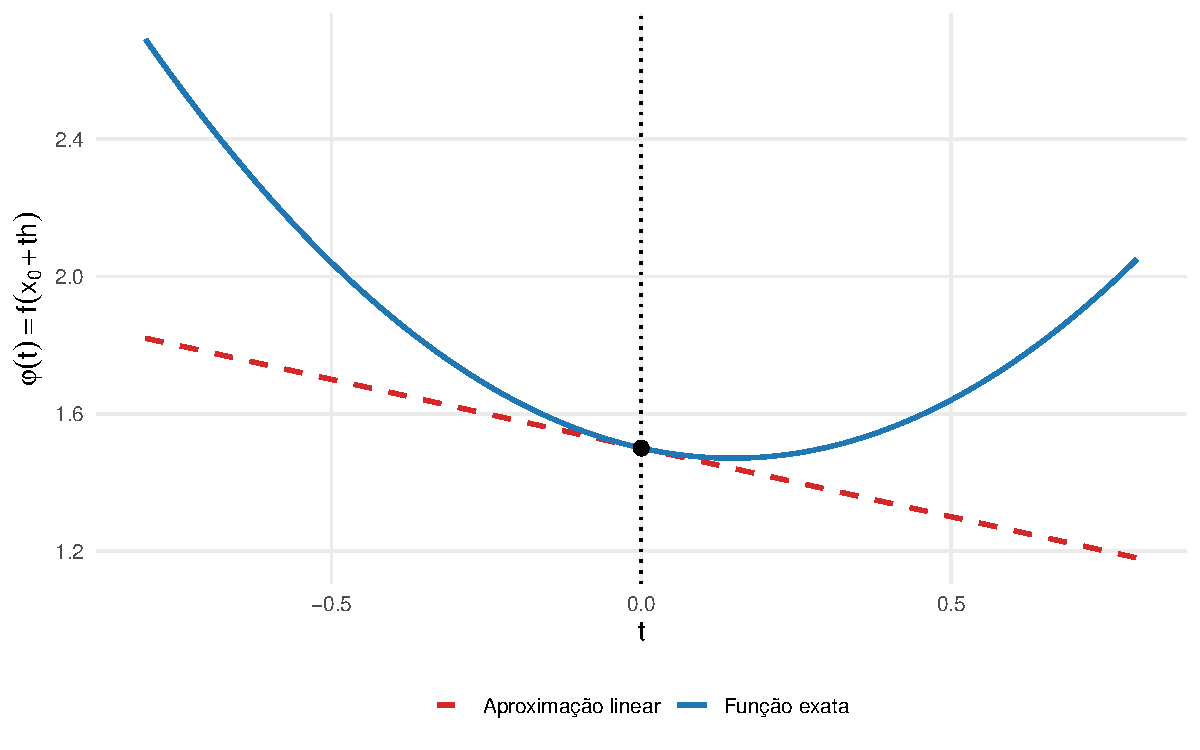
\includegraphics[keepaspectratio]{mod_1_calculo_files/figure-pdf/fig-aproximacao-linear-direcional-1.pdf}}

}

\caption{\label{fig-aproximacao-linear-direcional}Função exata ao longo
de uma direção e aproximação linear no ponto \(t=0\).}

\end{figure}%

No ponto \(t=0\), a função e sua aproximação linear possuem o mesmo
valor e a mesma inclinação. À medida que \(|t|\) aumenta, os termos de
segunda ordem passam a contribuir mais para a variação.

\subsection{Diferenciabilidade de funções
vetoriais}\label{diferenciabilidade-de-funuxe7uxf5es-vetoriais}

Para uma função

\[
\mathbf{g}:
\mathcal{U}
\subseteq
\mathbb{R}^{p}
\longrightarrow
\mathbb{R}^{q},
\]

a aproximação de primeira ordem é uma transformação linear de
\(\mathbb{R}^{p}\) em \(\mathbb{R}^{q}\).

\begin{definition}[Diferenciabilidade de uma função
vetorial]\protect\hypertarget{def-diferenciabilidade-vetorial}{}\label{def-diferenciabilidade-vetorial}

A função \(\mathbf{g}\) é diferenciável em um ponto interior

\[
\mathbf{x}
\in
\mathcal{U}
\]

quando existe uma matriz

\[
\mathbf{J}_{\mathbf{g}}(\mathbf{x})
\in
\mathbb{R}^{q\times p}
\]

tal que

\[
\mathbf{g}(\mathbf{x}+\mathbf{h})
-
\mathbf{g}(\mathbf{x})
=
\mathbf{J}_{\mathbf{g}}(\mathbf{x})
\mathbf{h}
+
\mathbf{r}_{\mathbf{x}}(\mathbf{h}),
\]

com

\[
\frac{
\left\|
\mathbf{r}_{\mathbf{x}}(\mathbf{h})
\right\|
}{
\|\mathbf{h}\|
}
\longrightarrow
0
\qquad
\text{quando}
\qquad
\|\mathbf{h}\|
\longrightarrow
0.
\]

\end{definition}

Assim,

\[
\mathbf{g}(\mathbf{x}+\mathbf{h})
\approx
\mathbf{g}(\mathbf{x})
+
\mathbf{J}_{\mathbf{g}}(\mathbf{x})
\mathbf{h},
\]

e o diferencial é

\[
d\mathbf{g}
=
\mathbf{J}_{\mathbf{g}}(\mathbf{x})
d\mathbf{x}.
\]

Para a transformação linear

\[
\mathbf{g}(\mathbf{x})
=
\mathbf{A}\mathbf{x},
\]

tem-se

\[
\mathbf{J}_{\mathbf{g}}(\mathbf{x})
=
\mathbf{A}
\]

em todos os pontos. Portanto,

\[
d\mathbf{g}
=
\mathbf{A}\,d\mathbf{x},
\]

e a aproximação linear é exata.

Gradiente e Jacobiana estão associados à mesma ideia de aproximação
linear local, mas correspondem a contradomínios diferentes. Para uma
função escalar, o gradiente fornece a representação vetorial da
aplicação linear que define o diferencial. Para uma função vetorial, a
Jacobiana fornece a representação matricial dessa aplicação linear.

\section{Gradiente, derivada direcional, Jacobiana e
Hessiana}\label{gradiente-derivada-direcional-jacobiana-e-hessiana}

\subsection{Gradiente e derivada
direcional}\label{gradiente-e-derivada-direcional}

Para uma função diferenciável

\[
f:
\mathbb{R}^{p}
\longrightarrow
\mathbb{R},
\]

o gradiente reúne as derivadas parciais:

\[
\nabla_{\mathbf{x}}f(\mathbf{x})
=
\begin{bmatrix}
\dfrac{\partial f}{\partial x_1}\\
\vdots\\
\dfrac{\partial f}{\partial x_p}
\end{bmatrix}.
\]

A derivada parcial em relação a \(x_j\) mede a variação da função na
direção do vetor canônico \(\mathbf{e}_j\). A variação em uma direção
arbitrária é descrita pela derivada direcional.

\begin{definition}[Derivada
direcional]\protect\hypertarget{def-derivada-direcional}{}\label{def-derivada-direcional}

Seja

\[
\mathbf{u}
\in
\mathbb{R}^{p}.
\]

A derivada direcional de \(f\) no ponto \(\mathbf{x}\) na direção de
\(\mathbf{u}\) é

\[
D_{\mathbf{u}}f(\mathbf{x})
=
\lim_{t\to0}
\frac{
f(\mathbf{x}+t\mathbf{u})
-
f(\mathbf{x})
}{
t
},
\]

quando esse limite existe.

\end{definition}

Considere a função de uma variável

\[
\varphi(t)
=
f(\mathbf{x}+t\mathbf{u}).
\]

Pela regra da cadeia,

\[
\begin{aligned}
\varphi'(0)
&=
\nabla_{\mathbf{x}}f(\mathbf{x})^{\top}
\frac{d}{dt}
\left(
\mathbf{x}+t\mathbf{u}
\right)
\bigg|_{t=0}\\
&=
\nabla_{\mathbf{x}}f(\mathbf{x})^{\top}
\mathbf{u}.
\end{aligned}
\]

Portanto, se \(f\) é diferenciável,

\[
D_{\mathbf{u}}f(\mathbf{x})
=
\nabla_{\mathbf{x}}f(\mathbf{x})^{\top}
\mathbf{u}.
\]

Quando \(\mathbf{u}\) é unitário, a derivada direcional mede a taxa de
variação por unidade de deslocamento.

Se \(\theta\) é o ângulo entre \(\nabla_{\mathbf{x}}f(\mathbf{x})\) e
\(\mathbf{u}\), então

\[
D_{\mathbf{u}}f(\mathbf{x})
=
\left\|
\nabla_{\mathbf{x}}f(\mathbf{x})
\right\|
\|\mathbf{u}\|
\cos\theta.
\]

Para \(\|\mathbf{u}\|=1\),

\[
D_{\mathbf{u}}f(\mathbf{x})
=
\left\|
\nabla_{\mathbf{x}}f(\mathbf{x})
\right\|
\cos\theta.
\]

\begin{proposition}[Direções de maior crescimento e
redução]\protect\hypertarget{prp-gradiente-crescimento}{}\label{prp-gradiente-crescimento}

Se \(f\) é diferenciável em \(\mathbf{x}\) e

\[
\nabla_{\mathbf{x}}f(\mathbf{x})
\neq
\mathbf{0},
\]

então, entre todas as direções unitárias,

\[
\max_{\|\mathbf{u}\|=1}
D_{\mathbf{u}}f(\mathbf{x})
=
\left\|
\nabla_{\mathbf{x}}f(\mathbf{x})
\right\|,
\]

e o máximo é atingido na direção

\[
\mathbf{u}_{\max}
=
\frac{
\nabla_{\mathbf{x}}f(\mathbf{x})
}{
\left\|
\nabla_{\mathbf{x}}f(\mathbf{x})
\right\|
}.
\]

A maior taxa de redução de primeira ordem ocorre na direção oposta:

\[
\mathbf{u}_{\min}
=
-
\frac{
\nabla_{\mathbf{x}}f(\mathbf{x})
}{
\left\|
\nabla_{\mathbf{x}}f(\mathbf{x})
\right\|
},
\]

com

\[
\min_{\|\mathbf{u}\|=1}
D_{\mathbf{u}}f(\mathbf{x})
=
-
\left\|
\nabla_{\mathbf{x}}f(\mathbf{x})
\right\|.
\]

(Apostol, 1969)

\end{proposition}

\begin{proof}
Pelo Teorema~\ref{thm-cauchy-schwarz},

\[
\begin{aligned}
D_{\mathbf{u}}f(\mathbf{x})
&=
\nabla_{\mathbf{x}}f(\mathbf{x})^{\top}
\mathbf{u}\\
&\leq
\left\|
\nabla_{\mathbf{x}}f(\mathbf{x})
\right\|
\|\mathbf{u}\|.
\end{aligned}
\]

Para \(\|\mathbf{u}\|=1\),

\[
D_{\mathbf{u}}f(\mathbf{x})
\leq
\left\|
\nabla_{\mathbf{x}}f(\mathbf{x})
\right\|.
\]

A igualdade ocorre quando \(\mathbf{u}\) possui a mesma direção e o
mesmo sentido do gradiente. Aplicando o mesmo argumento à direção
oposta, obtém-se o resultado para a maior taxa de redução de primeira
ordem.
\end{proof}

Se

\[
\nabla_{\mathbf{x}}f(\mathbf{x})
=
\mathbf{0},
\]

todas as derivadas direcionais de primeira ordem são nulas. Nesse caso,
a aproximação de primeira ordem não distingue direções de crescimento ou
redução, e o comportamento local passa a depender de termos de ordem
superior.

\subsection{Gradiente e conjuntos de
nível}\label{gradiente-e-conjuntos-de-nuxedvel}

Um conjunto de nível de \(f\) é definido por

\[
\mathcal{S}_c
=
\left\{
\mathbf{x}\in\mathbb{R}^{p}:
f(\mathbf{x})=c
\right\},
\]

em que \(c\) é constante.

Considere uma curva diferenciável

\[
\boldsymbol{\gamma}(t)
\]

contida em \(\mathcal{S}_c\). Então,

\[
f
\left(
\boldsymbol{\gamma}(t)
\right)
=
c.
\]

Derivando,

\[
\nabla_{\mathbf{x}}f
\left(
\boldsymbol{\gamma}(t)
\right)^{\top}
\boldsymbol{\gamma}'(t)
=
0.
\]

O vetor \(\boldsymbol{\gamma}'(t)\) é tangente ao conjunto de nível.
Portanto, o gradiente é ortogonal a todas as direções tangentes.

Quando

\[
\nabla_{\mathbf{x}}f(\mathbf{x})
\neq
\mathbf{0},
\]

o gradiente é um vetor normal ao conjunto de nível no ponto
\(\mathbf{x}\).

\begin{example}[Gradiente de uma função
quadrática]\protect\hypertarget{exm-gradiente-curva-nivel}{}\label{exm-gradiente-curva-nivel}

Considere

\[
f(x_1,x_2)
=
x_1^2
+
2x_2^2.
\]

O gradiente é

\[
\nabla_{\mathbf{x}}f(x_1,x_2)
=
\begin{bmatrix}
2x_1\\
4x_2
\end{bmatrix}.
\]

No ponto

\[
\mathbf{x}_0
=
\begin{bmatrix}
1\\
1/2
\end{bmatrix},
\]

tem-se

\[
\nabla_{\mathbf{x}}f(\mathbf{x}_0)
=
\begin{bmatrix}
2\\
2
\end{bmatrix}
\]

e

\[
\left\|
\nabla_{\mathbf{x}}f(\mathbf{x}_0)
\right\|
=
2\sqrt{2}.
\]

A direção de maior crescimento é

\[
\mathbf{u}_{\max}
=
\frac{1}{\sqrt{2}}
\begin{bmatrix}
1\\
1
\end{bmatrix}.
\]

Uma direção tangente à curva de nível é

\[
\mathbf{u}_{\mathrm{tan}}
=
\frac{1}{\sqrt{2}}
\begin{bmatrix}
-1\\
1
\end{bmatrix}.
\]

Como

\[
\nabla_{\mathbf{x}}f(\mathbf{x}_0)^{\top}
\mathbf{u}_{\mathrm{tan}}
=
0,
\]

a derivada direcional nessa direção é nula.

\end{example}

A Figura~\ref{fig-gradiente-curvas-nivel} representa as curvas de nível
da função, o gradiente e uma direção tangente no ponto \(\mathbf{x}_0\).

\begin{figure}

\centering{

\pandocbounded{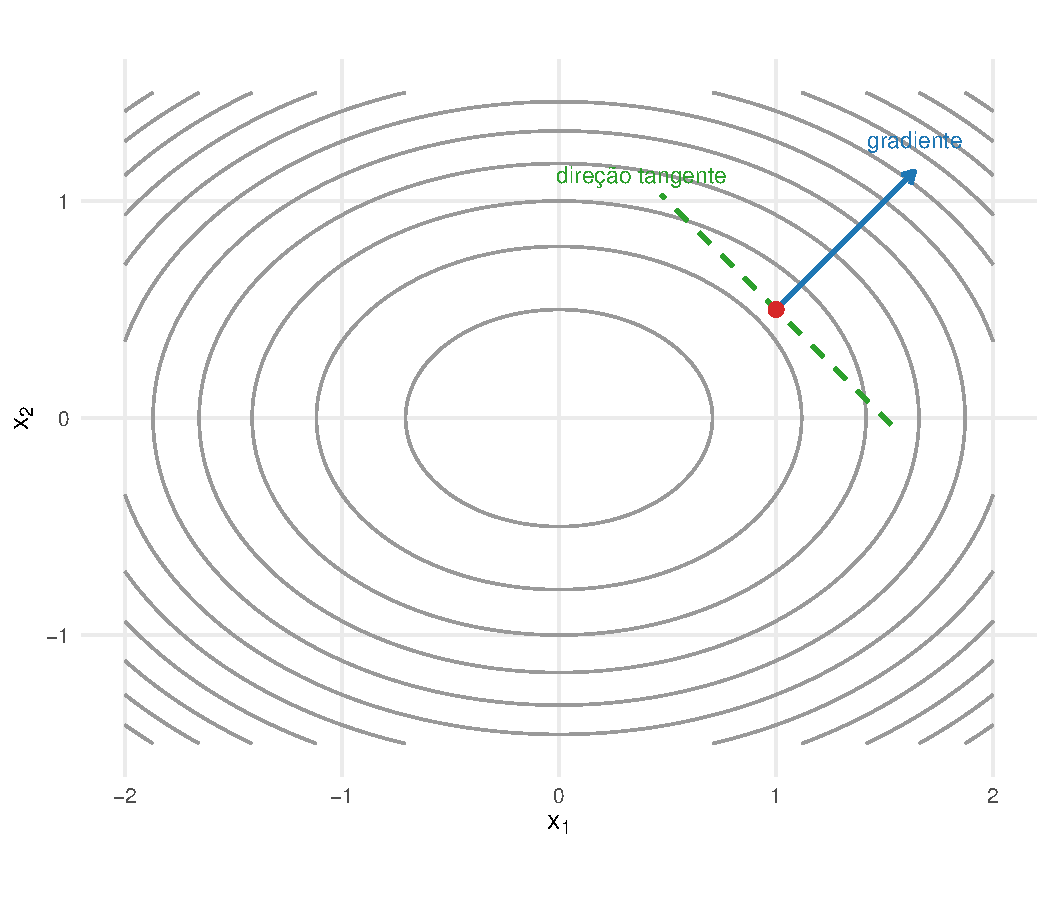
\includegraphics[keepaspectratio]{mod_1_calculo_files/figure-pdf/fig-gradiente-curvas-nivel-1.pdf}}

}

\caption{\label{fig-gradiente-curvas-nivel}O gradiente é perpendicular à
curva de nível e aponta na direção de maior crescimento local.}

\end{figure}%

A direção do gradiente depende do ponto. Para a função considerada, as
curvas de nível são elipses e o gradiente aponta para fora,
perpendicularmente à curva correspondente.

\subsection{Jacobiana}\label{jacobiana}

A derivada de uma função vetorial é representada por sua matriz
Jacobiana.

\begin{definition}[Matriz
Jacobiana]\protect\hypertarget{def-jacobiana}{}\label{def-jacobiana}

Seja

\[
\mathbf{g}:
\mathbb{R}^{p}
\longrightarrow
\mathbb{R}^{q},
\]

com

\[
\mathbf{g}(\mathbf{x})
=
\begin{bmatrix}
g_1(\mathbf{x})\\
\vdots\\
g_q(\mathbf{x})
\end{bmatrix}.
\]

Suponha que as derivadas parciais das componentes de \(\mathbf{g}\)
existam no ponto \(\mathbf{x}\). A matriz Jacobiana de \(\mathbf{g}\)
nesse ponto é

\[
\mathbf{J}_{\mathbf{g}}(\mathbf{x})
=
\begin{bmatrix}
\dfrac{\partial g_1}{\partial x_1}
&
\cdots
&
\dfrac{\partial g_1}{\partial x_p}
\\
\vdots
&
\ddots
&
\vdots
\\
\dfrac{\partial g_q}{\partial x_1}
&
\cdots
&
\dfrac{\partial g_q}{\partial x_p}
\end{bmatrix}
\in
\mathbb{R}^{q\times p}.
\]

\end{definition}

Cada linha da Jacobiana é o gradiente transposto de uma componente:

\[
\mathbf{J}_{\mathbf{g}}(\mathbf{x})
=
\begin{bmatrix}
\nabla_{\mathbf{x}}g_1(\mathbf{x})^{\top}\\
\vdots\\
\nabla_{\mathbf{x}}g_q(\mathbf{x})^{\top}
\end{bmatrix}.
\]

A aproximação de primeira ordem é

\[
\mathbf{g}(\mathbf{x}+\mathbf{h})
=
\mathbf{g}(\mathbf{x})
+
\mathbf{J}_{\mathbf{g}}(\mathbf{x})
\mathbf{h}
+
o(\|\mathbf{h}\|).
\]

A Jacobiana transforma uma pequena variação no domínio em uma
aproximação da variação correspondente no contradomínio.

\begin{example}[Jacobiana de uma função de \(\mathbb{R}^2\) em
\(\mathbb{R}^2\)]\protect\hypertarget{exm-jacobiana}{}\label{exm-jacobiana}

Considere

\[
\mathbf{g}(x_1,x_2)
=
\begin{bmatrix}
g_1\\
g_2
\end{bmatrix}
=
\begin{bmatrix}
x_1^2+x_2\\
x_1x_2
\end{bmatrix}.
\]

Os gradientes das componentes são

\[
\nabla_{\mathbf{x}}g_1
=
\begin{bmatrix}
2x_1\\
1
\end{bmatrix}
\]

e

\[
\nabla_{\mathbf{x}}g_2
=
\begin{bmatrix}
x_2\\
x_1
\end{bmatrix}.
\]

Logo,

\[
\mathbf{J}_{\mathbf{g}}(x_1,x_2)
=
\begin{bmatrix}
2x_1&1\\
x_2&x_1
\end{bmatrix}.
\]

No ponto

\[
\mathbf{x}_0
=
\begin{bmatrix}
1\\
2
\end{bmatrix},
\]

tem-se

\[
\mathbf{J}_{\mathbf{g}}(\mathbf{x}_0)
=
\begin{bmatrix}
2&1\\
2&1
\end{bmatrix}.
\]

Para uma pequena perturbação

\[
\mathbf{h}
=
\begin{bmatrix}
h_1\\
h_2
\end{bmatrix},
\]

a alteração é aproximada por

\[
\mathbf{g}(\mathbf{x}_0+\mathbf{h})
-
\mathbf{g}(\mathbf{x}_0)
\approx
\begin{bmatrix}
2&1\\
2&1
\end{bmatrix}
\begin{bmatrix}
h_1\\
h_2
\end{bmatrix}.
\]

\end{example}

Para uma transformação afim

\[
\mathbf{g}(\mathbf{x})
=
\mathbf{A}\mathbf{x}
+
\mathbf{b},
\]

a Jacobiana é constante:

\[
\mathbf{J}_{\mathbf{g}}(\mathbf{x})
=
\mathbf{A}.
\]

Assim, a parte linear local de uma transformação afim é exatamente a
matriz \(\mathbf{A}\), enquanto o termo de translação desaparece na
diferenciação.

\subsection{Regra da cadeia}\label{regra-da-cadeia}

A composição de funções exige a composição de suas aproximações
lineares.

\begin{theorem}[Regra da cadeia para funções
vetoriais]\protect\hypertarget{thm-regra-cadeia}{}\label{thm-regra-cadeia}

Considere funções diferenciáveis

\[
\mathbf{g}:
\mathbb{R}^{p}
\longrightarrow
\mathbb{R}^{q}
\]

e

\[
\mathbf{h}:
\mathbb{R}^{q}
\longrightarrow
\mathbb{R}^{r}.
\]

Para

\[
\mathbf{f}
=
\mathbf{h}\circ\mathbf{g},
\]

a Jacobiana é

\[
\mathbf{J}_{\mathbf{f}}(\mathbf{x})
=
\mathbf{J}_{\mathbf{h}}
\left(
\mathbf{g}(\mathbf{x})
\right)
\mathbf{J}_{\mathbf{g}}(\mathbf{x}).
\]

(Apostol, 1969)

\end{theorem}

As dimensões do produto são

\[
(r\times q)
(q\times p)
=
r\times p.
\]

A ordem do produto reflete a composição das aplicações lineares: sobre
uma perturbação \(\mathbf{h}_{\mathbf{x}}\in\mathbb{R}^p\), atua
primeiro \(\mathbf{J}_{\mathbf{g}}(\mathbf{x})\) e, sobre o resultado,
atua \(\mathbf{J}_{\mathbf{h}}(\mathbf{g}(\mathbf{x}))\). Por isso, na
representação matricial, a Jacobiana de \(\mathbf{h}\) aparece à
esquerda.

No caso de uma composição escalar

\[
f(\mathbf{x})
=
h
\left(
\mathbf{g}(\mathbf{x})
\right),
\]

em que

\[
h:
\mathbb{R}^{q}
\longrightarrow
\mathbb{R},
\]

a regra da cadeia assume a forma

\[
\nabla_{\mathbf{x}}f(\mathbf{x})
=
\mathbf{J}_{\mathbf{g}}(\mathbf{x})^{\top}
\nabla_{\mathbf{y}}h(\mathbf{y})
\bigg|_{
\mathbf{y}=\mathbf{g}(\mathbf{x})
}.
\]

\begin{example}[Gradiente de uma função
composta]\protect\hypertarget{exm-regra-cadeia}{}\label{exm-regra-cadeia}

Considere

\[
\mathbf{g}(\mathbf{x})
=
\mathbf{A}\mathbf{x}
-
\mathbf{b}
\]

e

\[
h(\mathbf{y})
=
\mathbf{y}^{\top}\mathbf{y}.
\]

A função composta é

\[
f(\mathbf{x})
=
\left\|
\mathbf{A}\mathbf{x}
-
\mathbf{b}
\right\|^2.
\]

Como

\[
\mathbf{J}_{\mathbf{g}}(\mathbf{x})
=
\mathbf{A}
\]

e

\[
\nabla_{\mathbf{y}}h(\mathbf{y})
=
2\mathbf{y},
\]

segue que

\[
\begin{aligned}
\nabla_{\mathbf{x}}f(\mathbf{x})
&=
\mathbf{A}^{\top}
\left[
2
\left(
\mathbf{A}\mathbf{x}
-
\mathbf{b}
\right)
\right]\\
&=
2\mathbf{A}^{\top}
\left(
\mathbf{A}\mathbf{x}
-
\mathbf{b}
\right).
\end{aligned}
\]

Essa expressão será retomada no estudo das funções de mínimos quadrados.

\end{example}

\subsection{Hessiana}\label{hessiana}

A Hessiana descreve a variação local do gradiente.

\begin{definition}[Matriz
Hessiana]\protect\hypertarget{def-hessiana}{}\label{def-hessiana}

Seja

\[
f:
\mathbb{R}^{p}
\longrightarrow
\mathbb{R}
\]

uma função com derivadas parciais de segunda ordem no ponto considerado.
Sua matriz Hessiana é

\[
\nabla_{\mathbf{x}}^2f(\mathbf{x})
=
\begin{bmatrix}
\dfrac{\partial^2f}{\partial x_1^2}
&
\cdots
&
\dfrac{\partial^2f}{\partial x_1\partial x_p}
\\
\vdots
&
\ddots
&
\vdots
\\
\dfrac{\partial^2f}{\partial x_p\partial x_1}
&
\cdots
&
\dfrac{\partial^2f}{\partial x_p^2}
\end{bmatrix}
\in
\mathbb{R}^{p\times p}.
\]

\end{definition}

A Hessiana é a Jacobiana do gradiente:

\[
\nabla_{\mathbf{x}}^2f(\mathbf{x})
=
\mathbf{J}_{\nabla f}(\mathbf{x}).
\]

Se as derivadas parciais de segunda ordem são contínuas em uma
vizinhança do ponto, então

\[
\frac{
\partial^2f
}{
\partial x_i\partial x_j
}
=
\frac{
\partial^2f
}{
\partial x_j\partial x_i
},
\]

e a Hessiana é simétrica:

\[
\nabla_{\mathbf{x}}^2f(\mathbf{x})
=
\nabla_{\mathbf{x}}^2f(\mathbf{x})^{\top}.
\]

O segundo diferencial é

\[
d^2f
=
d\mathbf{x}^{\top}
\nabla_{\mathbf{x}}^2f(\mathbf{x})
d\mathbf{x}.
\] O segundo diferencial é uma forma quadrática no incremento
\(d\mathbf{x}\) e descreve a contribuição local de segunda ordem da
função.

Para uma direção \(\mathbf{u}\), considere novamente

\[
\varphi(t)
=
f(\mathbf{x}+t\mathbf{u}).
\]

A primeira derivada é

\[
\varphi'(0)
=
\nabla_{\mathbf{x}}f(\mathbf{x})^{\top}
\mathbf{u}.
\]

A segunda derivada é

\[
\varphi''(0)
=
\mathbf{u}^{\top}
\nabla_{\mathbf{x}}^2f(\mathbf{x})
\mathbf{u}.
\]

Essa forma quadrática representa a segunda taxa de variação de \(f\) ao
longo da reta que passa por \(\mathbf{x}\) na direção \(\mathbf{u}\) e
fornece a medida de curvatura direcional utilizada neste capítulo.

\begin{example}[Hessiana de uma função
quadrática]\protect\hypertarget{exm-hessiana-funcao-quadratica}{}\label{exm-hessiana-funcao-quadratica}

Considere

\[
f(x_1,x_2)
=
x_1^2
+
2x_2^2.
\]

O gradiente é

\[
\nabla_{\mathbf{x}}f(x_1,x_2)
=
\begin{bmatrix}
2x_1\\
4x_2
\end{bmatrix}.
\]

A Hessiana é

\[
\nabla_{\mathbf{x}}^2f(x_1,x_2)
=
\begin{bmatrix}
2&0\\
0&4
\end{bmatrix}.
\]

Para

\[
\mathbf{u}
=
\begin{bmatrix}
u_1\\
u_2
\end{bmatrix},
\]

a curvatura direcional é

\[
\begin{aligned}
\mathbf{u}^{\top}
\nabla_{\mathbf{x}}^2f
\mathbf{u}
&=
\begin{bmatrix}
u_1&u_2
\end{bmatrix}
\begin{bmatrix}
2&0\\
0&4
\end{bmatrix}
\begin{bmatrix}
u_1\\
u_2
\end{bmatrix}\\
&=
2u_1^2
+
4u_2^2.
\end{aligned}
\]

Ela é positiva para todo vetor não nulo. Para vetores unitários, a
segunda taxa de variação é maior nas direções com maior componente em
módulo no segundo eixo.

\end{example}

Para a função quadrática

\[
f(\mathbf{x})
=
\frac{1}{2}
\mathbf{x}^{\top}
\mathbf{A}
\mathbf{x}
-
\mathbf{b}^{\top}\mathbf{x}
+
c,
\]

com \(\mathbf{A}\) simétrica,

\[
\nabla_{\mathbf{x}}f(\mathbf{x})
=
\mathbf{A}\mathbf{x}
-
\mathbf{b}
\]

e

\[
\nabla_{\mathbf{x}}^2f(\mathbf{x})
=
\mathbf{A}.
\]

A curvatura da função é determinada pela matriz \(\mathbf{A}\). A
relação entre a Hessiana, a aproximação de segunda ordem, a convexidade
e a classificação de pontos estacionários será desenvolvida na próxima
seção.

\section{Aproximações de Taylor e classificação
local}\label{aproximauxe7uxf5es-de-taylor-e-classificauxe7uxe3o-local}

\subsection{Aproximação de Taylor de primeira
ordem}\label{aproximauxe7uxe3o-de-taylor-de-primeira-ordem}

A diferenciabilidade fornece uma aproximação linear da função em uma
vizinhança de um ponto.

Para

\[
f:
\mathbb{R}^{p}
\longrightarrow
\mathbb{R},
\]

diferenciável em \(\mathbf{x}_0\),

\[
f(\mathbf{x}_0+\mathbf{h})
=
f(\mathbf{x}_0)
+
\nabla_{\mathbf{x}}f(\mathbf{x}_0)^{\top}\mathbf{h}
+
o(\|\mathbf{h}\|).
\]

Tomando

\[
\mathbf{h}
=
\mathbf{x}-\mathbf{x}_0,
\]

obtém-se

\[
f(\mathbf{x})
\approx
f(\mathbf{x}_0)
+
\nabla_{\mathbf{x}}f(\mathbf{x}_0)^{\top}
\left(
\mathbf{x}-\mathbf{x}_0
\right).
\]

Essa é a aproximação de Taylor de primeira ordem.

Para funções de uma variável, ela corresponde à reta tangente. Para
funções de duas variáveis, corresponde ao plano tangente. Em dimensão
geral, corresponde a uma função afim que aproxima localmente \(f\).

\begin{example}[Aproximação linear de uma função
quadrática]\protect\hypertarget{exm-taylor-primeira-ordem}{}\label{exm-taylor-primeira-ordem}

Considere

\[
f(x_1,x_2)
=
x_1^2
+
2x_2^2
\]

e o ponto

\[
\mathbf{x}_0
=
\begin{bmatrix}
1\\
1/2
\end{bmatrix}.
\]

Tem-se

\[
f(\mathbf{x}_0)
=
1^2
+
2
\left(
\frac12
\right)^2
=
\frac32
\]

e

\[
\nabla_{\mathbf{x}}f(\mathbf{x}_0)
=
\begin{bmatrix}
2\\
2
\end{bmatrix}.
\]

A aproximação de primeira ordem é

\[
\begin{aligned}
f(\mathbf{x})
&\approx
\frac32
+
\begin{bmatrix}
2&2
\end{bmatrix}
\left[
\begin{bmatrix}
x_1\\
x_2
\end{bmatrix}
-
\begin{bmatrix}
1\\
1/2
\end{bmatrix}
\right]\\
&=
\frac32
+
2(x_1-1)
+
2
\left(
x_2-\frac12
\right).
\end{aligned}
\]

\end{example}

A aproximação linear descreve a variação determinada pelo gradiente. Ela
não representa a curvatura da função.

\subsection{Aproximação de Taylor de segunda
ordem}\label{aproximauxe7uxe3o-de-taylor-de-segunda-ordem}

Quando \(f\) é duas vezes diferenciável, a Hessiana permite incorporar a
curvatura local.

\begin{theorem}[Expansão de Taylor de segunda
ordem]\protect\hypertarget{thm-taylor-segunda-ordem}{}\label{thm-taylor-segunda-ordem}

Se

\[
f:
\mathbb{R}^{p}
\longrightarrow
\mathbb{R}
\]

possui derivadas de segunda ordem contínuas em uma vizinhança de
\(\mathbf{x}_0\), então

\[
\begin{aligned}
f(\mathbf{x}_0+\mathbf{h})
&=
f(\mathbf{x}_0)
+
\nabla_{\mathbf{x}}f(\mathbf{x}_0)^{\top}\mathbf{h}\\
&\quad+
\frac12
\mathbf{h}^{\top}
\nabla_{\mathbf{x}}^2f(\mathbf{x}_0)
\mathbf{h}
+
o(\|\mathbf{h}\|^2).
\end{aligned}
\]

(Apostol, 1969)

\end{theorem}

Em termos de \(\mathbf{x}-\mathbf{x}_0\),

\[
\begin{aligned}
f(\mathbf{x})
&\approx
f(\mathbf{x}_0)
+
\nabla_{\mathbf{x}}f(\mathbf{x}_0)^{\top}
\left(
\mathbf{x}-\mathbf{x}_0
\right)\\
&\quad+
\frac12
\left(
\mathbf{x}-\mathbf{x}_0
\right)^{\top}
\nabla_{\mathbf{x}}^2f(\mathbf{x}_0)
\left(
\mathbf{x}-\mathbf{x}_0
\right).
\end{aligned}
\]

Os três termos possuem funções distintas:

\begin{itemize}
\tightlist
\item
  \(f(\mathbf{x}_0)\) determina o nível da aproximação;
\item
  o gradiente determina a variação local de primeira ordem;
\item
  a Hessiana determina a variação local de segunda ordem.
\end{itemize}

Quando

\[
\nabla_{\mathbf{x}}f(\mathbf{x}_0)
=
\mathbf{0},
\]

o termo linear desaparece. Se a forma quadrática associada à Hessiana é
não degenerada, ela fornece o termo dominante da variação local. Quando
essa forma se anula em alguma direção, termos de ordem superior podem
ser necessários para determinar o comportamento da função.

\begin{example}[Expansão de uma função
quadrática]\protect\hypertarget{exm-taylor-segunda-ordem}{}\label{exm-taylor-segunda-ordem}

Considere

\[
f(\mathbf{x})
=
\frac12
\mathbf{x}^{\top}
\mathbf{A}
\mathbf{x}
-
\mathbf{b}^{\top}\mathbf{x}
+
c,
\]

com \(\mathbf{A}\) simétrica.

O gradiente é

\[
\nabla_{\mathbf{x}}f(\mathbf{x})
=
\mathbf{A}\mathbf{x}
-
\mathbf{b},
\]

e a Hessiana é

\[
\nabla_{\mathbf{x}}^2f(\mathbf{x})
=
\mathbf{A}.
\]

Como a função é quadrática, a expansão de Taylor de segunda ordem é
exata:

\[
\begin{aligned}
f(\mathbf{x}_0+\mathbf{h})
&=
f(\mathbf{x}_0)
+
\left(
\mathbf{A}\mathbf{x}_0-\mathbf{b}
\right)^{\top}\mathbf{h}\\
&\quad+
\frac12
\mathbf{h}^{\top}\mathbf{A}\mathbf{h}.
\end{aligned}
\]

Não existe termo residual de ordem superior.

\end{example}

\subsection{Pontos estacionários}\label{pontos-estacionuxe1rios}

\begin{definition}[Ponto
estacionário]\protect\hypertarget{def-ponto-estacionario}{}\label{def-ponto-estacionario}

Um ponto

\[
\mathbf{x}^{\star}
\]

é estacionário para uma função diferenciável \(f\) quando

\[
\nabla_{\mathbf{x}}f
\left(
\mathbf{x}^{\star}
\right)
=
\mathbf{0}.
\]

\end{definition}

Em um ponto estacionário, todas as derivadas direcionais de primeira
ordem são nulas:

\[
D_{\mathbf{u}}f
\left(
\mathbf{x}^{\star}
\right)
=
0
\]

para toda direção \(\mathbf{u}\).

\begin{proposition}[Condição necessária de primeira
ordem]\protect\hypertarget{prp-condicao-primeira-ordem-extremo-local}{}\label{prp-condicao-primeira-ordem-extremo-local}

Se \(f\) é diferenciável em um ponto interior \(\mathbf{x}^{\star}\) de
seu domínio e possui nesse ponto um máximo ou mínimo local, então

\[
\nabla_{\mathbf{x}}f
\left(
\mathbf{x}^{\star}
\right)
=
\mathbf{0}.
\]

\end{proposition}

\begin{proof}
Se

\[
\nabla_{\mathbf{x}}f
\left(
\mathbf{x}^{\star}
\right)
\neq
\mathbf{0},
\]

considere a direção unitária

\[
\mathbf{u}
=
\frac{
\nabla_{\mathbf{x}}f
\left(
\mathbf{x}^{\star}
\right)
}{
\left\|
\nabla_{\mathbf{x}}f
\left(
\mathbf{x}^{\star}
\right)
\right\|
}.
\]

Então,

\[
D_{\mathbf{u}}f
\left(
\mathbf{x}^{\star}
\right)
=
\left\|
\nabla_{\mathbf{x}}f
\left(
\mathbf{x}^{\star}
\right)
\right\|
>
0,
\]

enquanto

\[
D_{-\mathbf{u}}f
\left(
\mathbf{x}^{\star}
\right)
=
-
\left\|
\nabla_{\mathbf{x}}f
\left(
\mathbf{x}^{\star}
\right)
\right\|
<
0.
\]

Assim, existem direções locais de aumento e de redução, o que contradiz
a existência de um extremo local interior. Portanto,

\[
\nabla_{\mathbf{x}}f
\left(
\mathbf{x}^{\star}
\right)
=
\mathbf{0}.
\]
\end{proof}

Como

\[
\nabla_{\mathbf{x}}f
\left(
\mathbf{x}^{\star}
\right)
=
\mathbf{0},
\]

tem-se

\[
D_{\mathbf{u}}f
\left(
\mathbf{x}^{\star}
\right)
=
0
\]

para toda direção \(\mathbf{u}\).

A recíproca da proposição anterior não é verdadeira em geral: um ponto
estacionário pode ser mínimo local, máximo local ou ponto de sela.

\subsection{Classificação pela
Hessiana}\label{classificauxe7uxe3o-pela-hessiana}

\begin{theorem}[Teste da Hessiana em um ponto
estacionário]\protect\hypertarget{thm-classificacao-hessiana}{}\label{thm-classificacao-hessiana}

Considere uma função duas vezes continuamente diferenciável em uma
vizinhança de um ponto estacionário \(\mathbf{x}^{\star}\).

Se

\[
\nabla_{\mathbf{x}}^2f
\left(
\mathbf{x}^{\star}
\right)
\succ
\mathbf{0},
\]

então \(\mathbf{x}^{\star}\) é um mínimo local estrito.

Se

\[
\nabla_{\mathbf{x}}^2f
\left(
\mathbf{x}^{\star}
\right)
\prec
\mathbf{0},
\]

então \(\mathbf{x}^{\star}\) é um máximo local estrito.

Se

\[
\nabla_{\mathbf{x}}^2f
\left(
\mathbf{x}^{\star}
\right)
\]

é indefinida, então \(\mathbf{x}^{\star}\) é um ponto de sela.

Se a Hessiana é apenas semidefinida positiva ou semidefinida negativa, o
teste pode ser inconclusivo. (Apostol, 1969)

\end{theorem}

\begin{proof}
Como

\[
\nabla_{\mathbf{x}}f
\left(
\mathbf{x}^{\star}
\right)
=
\mathbf{0},
\]

a expansão de Taylor fornece

\[
f
\left(
\mathbf{x}^{\star}+\mathbf{h}
\right)
-
f
\left(
\mathbf{x}^{\star}
\right)
=
\frac12
\mathbf{h}^{\top}
\nabla_{\mathbf{x}}^2f
\left(
\mathbf{x}^{\star}
\right)
\mathbf{h}
+
o(\|\mathbf{h}\|^2).
\]

Considere inicialmente

\[
\mathbf{H}
=
\nabla_{\mathbf{x}}^2f
\left(
\mathbf{x}^{\star}
\right)
\succ
\mathbf{0}.
\]

Como \(\mathbf{H}\) é simétrica e positiva definida, seu menor autovalor
satisfaz

\[
\lambda_{\min}(\mathbf{H})
>
0.
\]

Portanto,

\[
\mathbf{h}^{\top}\mathbf{H}\mathbf{h}
\geq
\lambda_{\min}(\mathbf{H})
\|\mathbf{h}\|^2.
\]

Além disso,

\[
o(\|\mathbf{h}\|^2)
=
\varepsilon(\mathbf{h})
\|\mathbf{h}\|^2,
\]

com

\[
\varepsilon(\mathbf{h})
\longrightarrow
0
\]

quando \(\mathbf{h}\to\mathbf{0}\).

Logo, para \(\mathbf{h}\) suficientemente pequeno,

\[
\left|
\varepsilon(\mathbf{h})
\right|
<
\frac14
\lambda_{\min}(\mathbf{H}).
\]

Assim,

\[
\begin{aligned}
f
\left(
\mathbf{x}^{\star}+\mathbf{h}
\right)
-
f
\left(
\mathbf{x}^{\star}
\right)
&\geq
\frac12
\lambda_{\min}(\mathbf{H})
\|\mathbf{h}\|^2
-
\frac14
\lambda_{\min}(\mathbf{H})
\|\mathbf{h}\|^2\\
&=
\frac14
\lambda_{\min}(\mathbf{H})
\|\mathbf{h}\|^2\\
&>
0
\end{aligned}
\]

para todo \(\mathbf{h}\neq\mathbf{0}\) suficientemente pequeno.
Portanto, \(\mathbf{x}^{\star}\) é um mínimo local estrito.

O caso de Hessiana negativa definida é obtido aplicando o mesmo
argumento a \(-f\), produzindo um máximo local estrito.

Se a Hessiana é indefinida, existem vetores unitários \(\mathbf{u}_1\) e
\(\mathbf{u}_2\) tais que

\[
\mathbf{u}_1^{\top}
\mathbf{H}
\mathbf{u}_1
>
0
\]

e

\[
\mathbf{u}_2^{\top}
\mathbf{H}
\mathbf{u}_2
<
0.
\]

Considere perturbações da forma

\[
\mathbf{h}
=
t\mathbf{u}_j.
\]

Então,

\[
f
\left(
\mathbf{x}^{\star}
+
t\mathbf{u}_j
\right)
-
f
\left(
\mathbf{x}^{\star}
\right)
=
\frac12
t^2
\mathbf{u}_j^{\top}
\mathbf{H}
\mathbf{u}_j
+
o(t^2).
\]

Para \(|t|\) suficientemente pequeno, o sinal dessa diferença coincide
com o sinal da forma quadrática. Assim, a função assume valores maiores
que

\[
f
\left(
\mathbf{x}^{\star}
\right)
\]

em uma direção e menores em outra, arbitrariamente próximos de
\(\mathbf{x}^{\star}\). Portanto, \(\mathbf{x}^{\star}\) é um ponto de
sela.
\end{proof}

\begin{example}[Mínimo, máximo e ponto de
sela]\protect\hypertarget{exm-classificacao-pontos}{}\label{exm-classificacao-pontos}

Considere as funções

\[
f_1(x_1,x_2)
=
x_1^2+x_2^2,
\]

\[
f_2(x_1,x_2)
=
-
x_1^2-x_2^2
\]

e

\[
f_3(x_1,x_2)
=
x_1^2-x_2^2.
\]

As três possuem ponto estacionário na origem.

Para \(f_1\),

\[
\nabla_{\mathbf{x}}^2f_1
=
\begin{bmatrix}
2&0\\
0&2
\end{bmatrix}
\succ
\mathbf{0}.
\]

Logo, a origem é um mínimo estrito.

Para \(f_2\),

\[
\nabla_{\mathbf{x}}^2f_2
=
\begin{bmatrix}
-2&0\\
0&-2
\end{bmatrix}
\prec
\mathbf{0}.
\]

Logo, a origem é um máximo estrito.

Para \(f_3\),

\[
\nabla_{\mathbf{x}}^2f_3
=
\begin{bmatrix}
2&0\\
0&-2
\end{bmatrix}.
\]

A Hessiana possui um autovalor positivo e outro negativo. Portanto, a
origem é um ponto de sela.

\end{example}

A Figura~\ref{fig-curvatura-hessiana} compara as curvas de nível dos
três casos.

\begin{figure}

\centering{

\pandocbounded{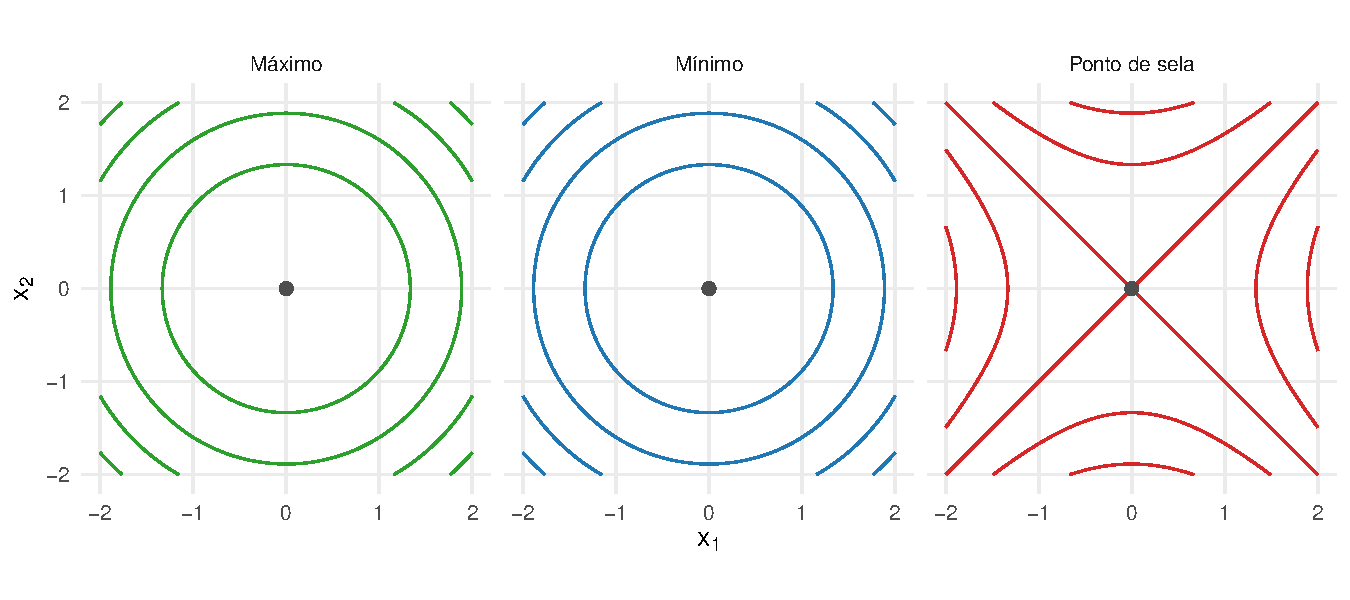
\includegraphics[keepaspectratio]{mod_1_calculo_files/figure-pdf/fig-curvatura-hessiana-1.pdf}}

}

\caption{\label{fig-curvatura-hessiana}Curvas de nível associadas a um
mínimo, um máximo e um ponto de sela.}

\end{figure}%

\subsection{Caso inconclusivo}\label{caso-inconclusivo}

Considere

\[
f(x_1,x_2)
=
x_1^4+x_2^4.
\]

A origem é um ponto estacionário e

\[
\nabla_{\mathbf{x}}^2f(0,0)
=
\begin{bmatrix}
0&0\\
0&0
\end{bmatrix}.
\]

A Hessiana é semidefinida positiva, mas não positiva definida. Ainda
assim,

\[
f(x_1,x_2)
\geq
0
\]

para todos os pontos, com igualdade somente na origem. Portanto, a
origem é um mínimo estrito.

Considere agora

\[
g(x_1,x_2)
=
x_1^4-x_2^4.
\]

A Hessiana na origem também é nula. Entretanto, a função assume valores
positivos e negativos em qualquer vizinhança da origem. O ponto é de
sela.

Esses exemplos mostram que, quando o termo quadrático se anula em
determinadas direções, é necessário examinar termos de ordem superior ou
utilizar outro argumento.

\section{Convexidade e concavidade}\label{convexidade-e-concavidade}

\subsection{Conjuntos convexos}\label{conjuntos-convexos}

\begin{definition}[Conjunto
convexo]\protect\hypertarget{def-conjunto-convexo}{}\label{def-conjunto-convexo}

Um conjunto

\[
\mathcal{C}
\subseteq
\mathbb{R}^{p}
\]

é convexo quando, para quaisquer

\[
\mathbf{x},\mathbf{y}
\in
\mathcal{C}
\]

e

\[
t\in[0,1],
\]

tem-se

\[
t\mathbf{x}
+
(1-t)\mathbf{y}
\in
\mathcal{C}.
\]

\end{definition}

O vetor

\[
t\mathbf{x}
+
(1-t)\mathbf{y}
\]

percorre o segmento de reta entre \(\mathbf{x}\) e \(\mathbf{y}\).
Assim, um conjunto é convexo quando contém todos os segmentos que ligam
seus pontos.

Subespaços, conjuntos afins como hiperplanos, bolas e regiões
elipsoidais da forma

\[
\left\{
\mathbf{x}:
\left(
\mathbf{x}-\boldsymbol{\mu}
\right)^{\top}
\mathbf{A}
\left(
\mathbf{x}-\boldsymbol{\mu}
\right)
\leq c
\right\},
\]

com \(\mathbf{A}\succ\mathbf{0}\) e \(c>0\), e o cone das matrizes
positivas definidas são exemplos de conjuntos convexos.

\subsection{Funções convexas}\label{funuxe7uxf5es-convexas}

\begin{definition}[Função
convexa]\protect\hypertarget{def-funcao-convexa}{}\label{def-funcao-convexa}

Uma função

\[
f:
\mathcal{C}
\longrightarrow
\mathbb{R},
\]

definida em um conjunto convexo \(\mathcal{C}\), é convexa quando

\[
f
\left(
t\mathbf{x}
+
(1-t)\mathbf{y}
\right)
\leq
t f(\mathbf{x})
+
(1-t)f(\mathbf{y})
\]

para quaisquer \(\mathbf{x},\mathbf{y}\in\mathcal{C}\) e \(t\in[0,1]\).

\end{definition}

A função é estritamente convexa quando a desigualdade é estrita para
\(\mathbf{x}\neq\mathbf{y}\) e \(t\in(0,1)\).

Uma função é côncava quando \(-f\) é convexa.

Geometricamente, o gráfico de uma função convexa permanece abaixo das
cordas que ligam dois pontos de seu gráfico.

\subsection{Caracterização de primeira
ordem}\label{caracterizauxe7uxe3o-de-primeira-ordem}

\begin{theorem}[Critério de primeira ordem para
convexidade]\protect\hypertarget{thm-convexidade-primeira-ordem}{}\label{thm-convexidade-primeira-ordem}

Se \(f\) é diferenciável em um conjunto convexo aberto \(\mathcal{C}\),
então \(f\) é convexa se, e somente se,

\[
f(\mathbf{y})
\geq
f(\mathbf{x})
+
\nabla_{\mathbf{x}}f(\mathbf{x})^{\top}
\left(
\mathbf{y}-\mathbf{x}
\right)
\]

para quaisquer \(\mathbf{x},\mathbf{y}\in\mathcal{C}\).(Boyd;
Vandenberghe, 2004)

\end{theorem}

A expressão

\[
f(\mathbf{x})
+
\nabla_{\mathbf{x}}f(\mathbf{x})^{\top}
\left(
\mathbf{y}-\mathbf{x}
\right)
\]

é a aproximação afim determinada pelo plano tangente em \(\mathbf{x}\).
Para uma função convexa, essa aproximação é um limite inferior global.

\subsection{Caracterização pela
Hessiana}\label{caracterizauxe7uxe3o-pela-hessiana}

\begin{theorem}[Critério da Hessiana para
convexidade]\protect\hypertarget{thm-convexidade-hessiana}{}\label{thm-convexidade-hessiana}

Considere uma função

\[
f:
\mathcal{C}
\longrightarrow
\mathbb{R}
\]

duas vezes continuamente diferenciável em um conjunto convexo aberto

\[
\mathcal{C}
\subseteq
\mathbb{R}^{p}.
\]

Então, \(f\) é convexa em \(\mathcal{C}\) se, e somente se,

\[
\nabla_{\mathbf{x}}^2f(\mathbf{x})
\succeq
\mathbf{0}
\]

para todo

\[
\mathbf{x}
\in
\mathcal{C}.
\]

Analogamente, \(f\) é côncava em \(\mathcal{C}\) se, e somente se,

\[
\nabla_{\mathbf{x}}^2f(\mathbf{x})
\preceq
\mathbf{0}
\]

para todo

\[
\mathbf{x}
\in
\mathcal{C}.
\]

Além disso, se

\[
\nabla_{\mathbf{x}}^2f(\mathbf{x})
\succ
\mathbf{0}
\]

para todo \(\mathbf{x}\in\mathcal{C}\), então \(f\) é estritamente
convexa. Se

\[
\nabla_{\mathbf{x}}^2f(\mathbf{x})
\prec
\mathbf{0}
\]

para todo \(\mathbf{x}\in\mathcal{C}\), então \(f\) é estritamente
côncava.

(Boyd; Vandenberghe, 2004)

\end{theorem}

\begin{proof}
Considere dois pontos distintos

\[
\mathbf{x},
\mathbf{y}
\in
\mathcal{C}
\]

e defina

\[
g(t)
=
f
\left(
\mathbf{x}
+
t(\mathbf{y}-\mathbf{x})
\right),
\qquad
0\leq t\leq1.
\]

Como \(\mathcal{C}\) é convexo, todo o segmento entre \(\mathbf{x}\) e
\(\mathbf{y}\) pertence a \(\mathcal{C}\).

Pela regra da cadeia,

\[
g''(t)
=
(\mathbf{y}-\mathbf{x})^{\top}
\nabla_{\mathbf{x}}^2
f
\left(
\mathbf{x}
+
t(\mathbf{y}-\mathbf{x})
\right)
(\mathbf{y}-\mathbf{x}).
\]

Se

\[
\nabla_{\mathbf{x}}^2f(\mathbf{z})
\succeq
\mathbf{0}
\]

para todo \(\mathbf{z}\in\mathcal{C}\), então

\[
g''(t)\geq0,
\]

e, portanto, \(g\) é convexa em \([0,1]\). Como isso vale para qualquer
segmento contido em \(\mathcal{C}\), \(f\) é convexa.

Reciprocamente, se \(f\) é convexa, então a restrição de \(f\) a
qualquer reta é convexa. Para qualquer

\[
\mathbf{x}\in\mathcal{C}
\]

e qualquer direção

\[
\mathbf{u}\in\mathbb{R}^{p},
\]

considere

\[
h(t)
=
f(\mathbf{x}+t\mathbf{u})
\]

para \(t\) suficientemente próximo de zero. A convexidade de \(h\)
implica

\[
h''(0)\geq0.
\]

Como

\[
h''(0)
=
\mathbf{u}^{\top}
\nabla_{\mathbf{x}}^2f(\mathbf{x})
\mathbf{u},
\]

tem-se

\[
\mathbf{u}^{\top}
\nabla_{\mathbf{x}}^2f(\mathbf{x})
\mathbf{u}
\geq0
\]

para todo \(\mathbf{u}\). Logo,

\[
\nabla_{\mathbf{x}}^2f(\mathbf{x})
\succeq
\mathbf{0}.
\]

O resultado para funções côncavas segue aplicando o argumento a \(-f\).

Se a Hessiana é positiva definida em todo ponto, então, para
\(\mathbf{x}\neq\mathbf{y}\),

\[
g''(t)>0
\]

ao longo do segmento. Logo, \(g\) é estritamente convexa, e portanto
\(f\) é estritamente convexa. O caso de Hessiana negativa definida é
análogo.
\end{proof}

A positividade da Hessiana deve ser verificada para todos os pontos do
domínio considerado, e não somente em um ponto estacionário.

A condição

\[
\nabla_{\mathbf{x}}^2f(\mathbf{x})
\succ
\mathbf{0}
\]

em todo o domínio é suficiente para convexidade estrita, mas não é
necessária. Uma função estritamente convexa pode possuir Hessiana
singular em pontos isolados. Por exemplo,

\[
f(x)=x^4
\]

é estritamente convexa em \(\mathbb{R}\), embora

\[
f''(0)=0.
\]

\subsection{Consequências para
otimização}\label{consequuxeancias-para-otimizauxe7uxe3o}

\begin{proposition}[Pontos estacionários de funções
convexas]\protect\hypertarget{prp-convexidade-minimizacao}{}\label{prp-convexidade-minimizacao}

Se \(f\) é diferenciável e convexa em um conjunto convexo, qualquer
ponto

\[
\mathbf{x}^{\star}
\]

que satisfaça

\[
\nabla_{\mathbf{x}}f
\left(
\mathbf{x}^{\star}
\right)
=
\mathbf{0}
\]

é um mínimo global.

Se \(f\) é estritamente convexa e existe um ponto estacionário
\(\mathbf{x}^{\star}\), então esse ponto é o único minimizador global.
(Boyd; Vandenberghe, 2004)

\end{proposition}

\begin{proof}
Pela caracterização de primeira ordem,

\[
f(\mathbf{x})
\geq
f
\left(
\mathbf{x}^{\star}
\right)
+
\nabla_{\mathbf{x}}f
\left(
\mathbf{x}^{\star}
\right)^{\top}
\left(
\mathbf{x}-\mathbf{x}^{\star}
\right).
\]

Como o gradiente é nulo,

\[
f(\mathbf{x})
\geq
f
\left(
\mathbf{x}^{\star}
\right)
\]

para todo \(\mathbf{x}\) do domínio.

Se a função é estritamente convexa, a igualdade só pode ocorrer em
\(\mathbf{x}=\mathbf{x}^{\star}\).
\end{proof}

Essa propriedade diferencia a otimização convexa da otimização geral.
Para uma função convexa, não existem mínimos locais que deixem de ser
globais.

\subsection{Funções quadráticas}\label{funuxe7uxf5es-quadruxe1ticas}

Considere

\[
f(\mathbf{x})
=
\frac12
\mathbf{x}^{\top}\mathbf{A}\mathbf{x}
-
\mathbf{b}^{\top}\mathbf{x}
+
c,
\]

com \(\mathbf{A}\) simétrica.

Como

\[
\nabla_{\mathbf{x}}^2f(\mathbf{x})
=
\mathbf{A},
\]

tem-se:

\begin{itemize}
\tightlist
\item
  \(f\) é convexa se \(\mathbf{A}\succeq\mathbf{0}\);
\item
  \(f\) é estritamente convexa se \(\mathbf{A}\succ\mathbf{0}\);
\item
  \(f\) é côncava se \(\mathbf{A}\preceq\mathbf{0}\);
\item
  \(f\) é estritamente côncava se \(\mathbf{A}\prec\mathbf{0}\).
\end{itemize}

Se

\[
\mathbf{A}
\succ
\mathbf{0},
\]

o ponto estacionário satisfaz

\[
\mathbf{A}\mathbf{x}^{\star}
=
\mathbf{b},
\]

e

\[
\mathbf{x}^{\star}
=
\mathbf{A}^{-1}\mathbf{b}.
\]

Esse ponto é o único mínimo global.

Se

\[
\mathbf{A}
\succeq
\mathbf{0}
\]

é singular, a existência de minimizadores depende de \(\mathbf{b}\).

Quando

\[
\mathbf{b}
\in
\mathcal{C}(\mathbf{A}),
\]

o sistema

\[
\mathbf{A}\mathbf{x}
=
\mathbf{b}
\]

possui solução. Nesse caso, os minimizadores formam o conjunto afim

\[
\mathbf{x}_0
+
\mathcal{N}(\mathbf{A}),
\]

em que \(\mathbf{x}_0\) é uma solução particular.

Quando

\[
\mathbf{b}
\notin
\mathcal{C}(\mathbf{A}),
\]

a função é ilimitada inferiormente e não possui minimizador.

De fato, como \(\mathbf{A}\) é simétrica,

\[
\mathcal{C}(\mathbf{A})^{\perp}
=
\mathcal{N}(\mathbf{A}).
\]

Assim, existe

\[
\mathbf{z}
\in
\mathcal{N}(\mathbf{A})
\]

tal que

\[
\mathbf{b}^{\top}\mathbf{z}
\neq
0.
\]

Ao longo da reta

\[
\mathbf{x}=t\mathbf{z},
\]

o termo quadrático é nulo e

\[
f(t\mathbf{z})
=
-
t\mathbf{b}^{\top}\mathbf{z}
+
c,
\]

que pode tender a \(-\infty\) escolhendo o sinal apropriado de \(t\).

\section{Otimização sem
restrições}\label{otimizauxe7uxe3o-sem-restriuxe7uxf5es}

Um problema de minimização sem restrições possui a forma

\[
\min_{\mathbf{x}\in\mathbb{R}^{p}}
f(\mathbf{x}).
\]

A Proposição~\ref{prp-condicao-primeira-ordem-extremo-local} estabelece
a condição necessária de primeira ordem para extremos locais interiores,
enquanto o Teorema~\ref{thm-classificacao-hessiana} utiliza a Hessiana
para classificar pontos estacionários quando o teste de segunda ordem é
conclusivo.

No caso convexo, a Proposição~\ref{prp-convexidade-minimizacao} mostra
que um ponto estacionário é minimizador global. Esses resultados
fornecem as condições de otimalidade; a questão seguinte é construir um
procedimento iterativo para localizar esses pontos.

\subsection{Método de Newton}\label{muxe9todo-de-newton}

O método de Newton utiliza a aproximação quadrática local de \(f\).

Em torno de um ponto \(\mathbf{x}^{(t)}\),

\[
\begin{aligned}
f(\mathbf{x})
&\approx
f
\left(
\mathbf{x}^{(t)}
\right)
+
\nabla_{\mathbf{x}}f
\left(
\mathbf{x}^{(t)}
\right)^{\top}
\left(
\mathbf{x}
-
\mathbf{x}^{(t)}
\right)\\
&\quad+
\frac12
\left(
\mathbf{x}
-
\mathbf{x}^{(t)}
\right)^{\top}
\nabla_{\mathbf{x}}^2f
\left(
\mathbf{x}^{(t)}
\right)
\left(
\mathbf{x}
-
\mathbf{x}^{(t)}
\right).
\end{aligned}
\]

Defina

\[
\mathbf{g}^{(t)}
=
\nabla_{\mathbf{x}}f
\left(
\mathbf{x}^{(t)}
\right)
\]

e

\[
\mathbf{H}^{(t)}
=
\nabla_{\mathbf{x}}^2f
\left(
\mathbf{x}^{(t)}
\right).
\]

Escrevendo

\[
\mathbf{d}
=
\mathbf{x}
-
\mathbf{x}^{(t)},
\]

o modelo quadrático local pode ser representado por

\[
m_t(\mathbf{d})
=
f
\left(
\mathbf{x}^{(t)}
\right)
+
\left(
\mathbf{g}^{(t)}
\right)^{\top}
\mathbf{d}
+
\frac12
\mathbf{d}^{\top}
\mathbf{H}^{(t)}
\mathbf{d}.
\]

Seu gradiente em relação a \(\mathbf{d}\) é

\[
\nabla_{\mathbf{d}}m_t(\mathbf{d})
=
\mathbf{g}^{(t)}
+
\mathbf{H}^{(t)}
\mathbf{d}.
\]

Se

\[
\mathbf{H}^{(t)}
\succ
\mathbf{0},
\]

o modelo quadrático é estritamente convexo e possui um único
minimizador. Esse minimizador, denominado \textbf{direção de Newton},
satisfaz

\[
\mathbf{H}^{(t)}
\mathbf{d}^{(t)}
=
-
\mathbf{g}^{(t)}.
\]

Quando \(\mathbf{H}^{(t)}\) é invertível,

\[
\mathbf{d}^{(t)}
=
-
\left(
\mathbf{H}^{(t)}
\right)^{-1}
\mathbf{g}^{(t)}.
\]

A atualização de Newton com passo completo é

\[
\mathbf{x}^{(t+1)}
=
\mathbf{x}^{(t)}
+
\mathbf{d}^{(t)},
\]

ou, equivalentemente,

\[
\mathbf{x}^{(t+1)}
=
\mathbf{x}^{(t)}
-
\left[
\nabla_{\mathbf{x}}^2f
\left(
\mathbf{x}^{(t)}
\right)
\right]^{-1}
\nabla_{\mathbf{x}}f
\left(
\mathbf{x}^{(t)}
\right).
\]

Na implementação computacional, é preferível resolver o sistema linear

\[
\mathbf{H}^{(t)}
\mathbf{d}^{(t)}
=
-
\mathbf{g}^{(t)}
\]

sem calcular explicitamente a inversa da Hessiana.

Se a Hessiana é apenas invertível, mas não positiva definida, a solução
desse sistema é um ponto estacionário do modelo quadrático, mas pode não
ser seu minimizador. Nesse caso, a direção de Newton também pode deixar
de ser uma direção de descida para a função original.

\begin{proposition}[Direção de Newton como direção de
descida]\protect\hypertarget{prp-direcao-newton-descida}{}\label{prp-direcao-newton-descida}

Suponha que

\[
\nabla_{\mathbf{x}}f
\left(
\mathbf{x}^{(t)}
\right)
\neq
\mathbf{0}
\]

e

\[
\nabla_{\mathbf{x}}^2f
\left(
\mathbf{x}^{(t)}
\right)
\succ
\mathbf{0}.
\]

Então a direção de Newton \(\mathbf{d}^{(t)}\) é uma direção de descida
para \(f\) em \(\mathbf{x}^{(t)}\), isto é,

\[
\nabla_{\mathbf{x}}f
\left(
\mathbf{x}^{(t)}
\right)^{\top}
\mathbf{d}^{(t)}
<
0.
\]

\end{proposition}

\begin{proof}
Como

\[
\mathbf{d}^{(t)}
=
-
\left(
\mathbf{H}^{(t)}
\right)^{-1}
\mathbf{g}^{(t)},
\]

tem-se

\[
\begin{aligned}
\left(
\mathbf{g}^{(t)}
\right)^{\top}
\mathbf{d}^{(t)}
&=
-
\left(
\mathbf{g}^{(t)}
\right)^{\top}
\left(
\mathbf{H}^{(t)}
\right)^{-1}
\mathbf{g}^{(t)}.
\end{aligned}
\]

Como \(\mathbf{H}^{(t)}\succ\mathbf{0}\), também

\[
\left(
\mathbf{H}^{(t)}
\right)^{-1}
\succ
\mathbf{0}.
\]

Logo, para \(\mathbf{g}^{(t)}\neq\mathbf{0}\),

\[
\left(
\mathbf{g}^{(t)}
\right)^{\top}
\left(
\mathbf{H}^{(t)}
\right)^{-1}
\mathbf{g}^{(t)}
>
0,
\]

e, portanto,

\[
\left(
\mathbf{g}^{(t)}
\right)^{\top}
\mathbf{d}^{(t)}
<
0.
\]
\end{proof}

O passo completo corresponde a

\[
\alpha_t
=
1.
\]

Uma forma mais geral da atualização é

\[
\mathbf{x}^{(t+1)}
=
\mathbf{x}^{(t)}
+
\alpha_t
\mathbf{d}^{(t)},
\qquad
0<\alpha_t\leq1.
\]

A escolha de \(\alpha_t<1\) produz um passo de Newton amortecido. Esse
recurso pode ser utilizado quando o modelo quadrático local ainda não
representa adequadamente a função ao longo de um passo completo.

Assim, a construção da direção e a escolha do comprimento da etapa são
operações distintas. Métodos numéricos de otimização costumam combinar a
direção de Newton com procedimentos de controle da etapa (Boyd;
Vandenberghe, 2004).

\begin{example}[Newton para uma função
quadrática]\protect\hypertarget{exm-newton-funcao-quadratica}{}\label{exm-newton-funcao-quadratica}

Considere

\[
f(\mathbf{x})
=
\frac12
\mathbf{x}^{\top}\mathbf{A}\mathbf{x}
-
\mathbf{b}^{\top}\mathbf{x},
\]

com \(\mathbf{A}\succ\mathbf{0}\).

O gradiente é

\[
\nabla_{\mathbf{x}}f(\mathbf{x})
=
\mathbf{A}\mathbf{x}
-
\mathbf{b},
\]

e a Hessiana é

\[
\nabla_{\mathbf{x}}^2f(\mathbf{x})
=
\mathbf{A}.
\]

A atualização de Newton é

\[
\begin{aligned}
\mathbf{x}^{(t+1)}
&=
\mathbf{x}^{(t)}
-
\mathbf{A}^{-1}
\left(
\mathbf{A}\mathbf{x}^{(t)}
-
\mathbf{b}
\right)\\
&=
\mathbf{A}^{-1}\mathbf{b}.
\end{aligned}
\]

Assim, para uma função quadrática com Hessiana constante e positiva
definida, uma etapa completa de Newton conduz exatamente ao único
minimizador,

\[
\mathbf{x}^{\star}
=
\mathbf{A}^{-1}\mathbf{b},
\]

independentemente do ponto inicial.

\end{example}

\section{Otimização com restrições de
igualdade}\label{otimizauxe7uxe3o-com-restriuxe7uxf5es-de-igualdade}

Considere o problema

\[
\min_{\mathbf{x}\in\mathbb{R}^{p}}
f(\mathbf{x})
\]

sujeito a

\[
\mathbf{c}(\mathbf{x})
=
\mathbf{0},
\]

em que

\[
\mathbf{c}:
\mathbb{R}^{p}
\longrightarrow
\mathbb{R}^{m}
\]

é uma função vetorial de restrições:

\[
\mathbf{c}(\mathbf{x})
=
\begin{bmatrix}
c_1(\mathbf{x})\\
\vdots\\
c_m(\mathbf{x})
\end{bmatrix}.
\]

O conjunto viável é

\[
\mathcal{F}
=
\left\{
\mathbf{x}:
\mathbf{c}(\mathbf{x})
=
\mathbf{0}
\right\}.
\]

Em um ponto regular, as linhas da Jacobiana das restrições são
linearmente independentes. O espaço tangente ao conjunto viável é então

\[
\mathcal{T}_{\mathbf{x}}
=
\mathcal{N}
\left(
\mathbf{J}_{\mathbf{c}}(\mathbf{x})
\right).
\]

Portanto, uma direção tangente \(\mathbf{d}\) satisfaz

\[
\mathbf{J}_{\mathbf{c}}(\mathbf{x})
\mathbf{d}
=
\mathbf{0}.
\]

O espaço normal correspondente é

\[
\mathcal{T}_{\mathbf{x}}^{\perp}
=
\mathcal{C}
\left(
\mathbf{J}_{\mathbf{c}}(\mathbf{x})^{\top}
\right),
\]

isto é, o espaço gerado pelos gradientes das restrições.

Em um ótimo local regular \(\mathbf{x}^{\star}\), a derivada direcional
de \(f\) deve ser nula em todas as direções tangentes:

\[
\nabla_{\mathbf{x}}f
\left(
\mathbf{x}^{\star}
\right)^{\top}
\mathbf{d}
=
0
\]

para todo

\[
\mathbf{d}
\in
\mathcal{T}_{\mathbf{x}^{\star}}.
\]

Consequentemente,

\[
\nabla_{\mathbf{x}}f
\left(
\mathbf{x}^{\star}
\right)
\in
\mathcal{T}_{\mathbf{x}^{\star}}^{\perp}
=
\mathcal{C}
\left[
\mathbf{J}_{\mathbf{c}}
\left(
\mathbf{x}^{\star}
\right)^{\top}
\right].
\]

\subsection{Multiplicadores de
Lagrange}\label{multiplicadores-de-lagrange-1}

\begin{theorem}[Condição de
Lagrange]\protect\hypertarget{thm-multiplicadores-lagrange}{}\label{thm-multiplicadores-lagrange}

Considere funções continuamente diferenciáveis

\[
f:
\mathbb{R}^{p}
\longrightarrow
\mathbb{R}
\]

e

\[
\mathbf{c}:
\mathbb{R}^{p}
\longrightarrow
\mathbb{R}^{m}.
\]

Seja \(\mathbf{x}^{\star}\) um ótimo local do problema

\[
\min_{\mathbf{x}}
f(\mathbf{x})
\]

sujeito a

\[
\mathbf{c}(\mathbf{x})
=
\mathbf{0}.
\]

Suponha que as linhas da Jacobiana

\[
\mathbf{J}_{\mathbf{c}}
\left(
\mathbf{x}^{\star}
\right)
\]

sejam linearmente independentes.

Essa condição equivale a

\[
\operatorname{posto}
\left[
\mathbf{J}_{\mathbf{c}}
\left(
\mathbf{x}^{\star}
\right)
\right]
=
m.
\]

Então existe um vetor

\[
\boldsymbol{\lambda}^{\star}
\in
\mathbb{R}^{m}
\]

tal que

\[
\nabla_{\mathbf{x}}f
\left(
\mathbf{x}^{\star}
\right)
+
\mathbf{J}_{\mathbf{c}}
\left(
\mathbf{x}^{\star}
\right)^{\top}
\boldsymbol{\lambda}^{\star}
=
\mathbf{0}.
\]

(Apostol, 1969)

\end{theorem}

\begin{proof}
Como \(\mathbf{x}^{\star}\) é um ótimo local regular, a derivada
direcional da função objetivo é nula em todas as direções tangentes ao
conjunto viável. Portanto,

\[
\nabla_{\mathbf{x}}f
\left(
\mathbf{x}^{\star}
\right)^{\top}
\mathbf{d}
=
0
\]

para todo

\[
\mathbf{d}
\in
\mathcal{N}
\left[
\mathbf{J}_{\mathbf{c}}
\left(
\mathbf{x}^{\star}
\right)
\right].
\]

Logo,

\[
\nabla_{\mathbf{x}}f
\left(
\mathbf{x}^{\star}
\right)
\in
\mathcal{N}
\left[
\mathbf{J}_{\mathbf{c}}
\left(
\mathbf{x}^{\star}
\right)
\right]^{\perp}.
\]

Pelo Teorema~\ref{thm-ortogonalidade-espacos-fundamentais},

\[
\mathcal{N}
\left[
\mathbf{J}_{\mathbf{c}}
\left(
\mathbf{x}^{\star}
\right)
\right]^{\perp}
=
\mathcal{C}
\left[
\mathbf{J}_{\mathbf{c}}
\left(
\mathbf{x}^{\star}
\right)^{\top}
\right].
\]

Assim, existe um vetor

\[
\boldsymbol{\mu}^{\star}
\in
\mathbb{R}^{m}
\]

tal que

\[
\nabla_{\mathbf{x}}f
\left(
\mathbf{x}^{\star}
\right)
=
\mathbf{J}_{\mathbf{c}}
\left(
\mathbf{x}^{\star}
\right)^{\top}
\boldsymbol{\mu}^{\star}.
\]

Definindo

\[
\boldsymbol{\lambda}^{\star}
=
-
\boldsymbol{\mu}^{\star},
\]

obtém-se

\[
\nabla_{\mathbf{x}}f
\left(
\mathbf{x}^{\star}
\right)
+
\mathbf{J}_{\mathbf{c}}
\left(
\mathbf{x}^{\star}
\right)^{\top}
\boldsymbol{\lambda}^{\star}
=
\mathbf{0}.
\]
\end{proof}

A função lagrangiana é

\[
\mathcal{L}
\left(
\mathbf{x},
\boldsymbol{\lambda}
\right)
=
f(\mathbf{x})
+
\boldsymbol{\lambda}^{\top}
\mathbf{c}(\mathbf{x}).
\]

Sob a condição de regularidade do teorema, as condições necessárias de
primeira ordem podem ser escritas como

\[
\nabla_{\mathbf{x}}
\mathcal{L}
\left(
\mathbf{x},
\boldsymbol{\lambda}
\right)
=
\mathbf{0}
\]

e

\[
\nabla_{\boldsymbol{\lambda}}
\mathcal{L}
\left(
\mathbf{x},
\boldsymbol{\lambda}
\right)
=
\mathbf{c}(\mathbf{x})
=
\mathbf{0}.
\]

Essas condições identificam candidatos a ótimo restrito. No caso geral,
elas não são suficientes para garantir mínimo ou máximo. A classificação
exige condições adicionais sobre a função objetivo, as restrições e a
variação de segunda ordem nas direções tangentes.

Os multiplicadores ajustam a condição de gradiente nulo para levar em
conta as direções que não estão disponíveis devido às restrições.

\begin{example}[Otimização com restrição de
norma]\protect\hypertarget{exm-lagrange-restricao-norma}{}\label{exm-lagrange-restricao-norma}

Considere o problema

\[
\max_{\mathbf{x}}
\mathbf{a}^{\top}\mathbf{x},
\]

em que

\[
\mathbf{a}
\neq
\mathbf{0},
\]

sujeito à restrição

\[
\mathbf{x}^{\top}\mathbf{x}
=
1.
\]

A restrição exige que \(\mathbf{x}\) tenha norma euclidiana unitária:

\[
\|\mathbf{x}\|
=
1.
\]

Escrevendo-a na forma

\[
c(\mathbf{x})
=
\mathbf{x}^{\top}\mathbf{x}
-
1
=
0,
\]

o problema pode ser tratado pelos multiplicadores de Lagrange.

Para manter a formulação como um problema de minimização, considere a
função objetivo

\[
f(\mathbf{x})
=
-
\mathbf{a}^{\top}\mathbf{x}.
\]

A lagrangiana é

\[
\mathcal{L}(\mathbf{x},\lambda)
=
-
\mathbf{a}^{\top}\mathbf{x}
+
\lambda
\left(
\mathbf{x}^{\top}\mathbf{x}-1
\right).
\]

As condições de primeira ordem são obtidas diferenciando a lagrangiana
em relação a \(\mathbf{x}\) e ao multiplicador \(\lambda\).

Em relação a \(\mathbf{x}\),

\[
\nabla_{\mathbf{x}} \mathcal{L}(\mathbf{x},\lambda) = -\mathbf{a}+ 2\lambda\mathbf{x}.
\]

Portanto, em um ponto candidato à solução,

\[ - \mathbf{a} + 2\lambda\mathbf{x} = \mathbf{0},\]

de modo que

\[
\mathbf{x} = \frac{1}{2\lambda} \mathbf{a}.
\]

Em relação a \(\lambda\),

\[
\frac{
\partial
\mathcal{L}(\mathbf{x},\lambda)
}{
\partial\lambda
}
=
\mathbf{x}^{\top}\mathbf{x}-1.
\]

Assim, a segunda condição de primeira ordem simplesmente recupera a
restrição:

\[
\mathbf{x}^{\top}\mathbf{x}
=
1.
\]

Substituindo

\[
\mathbf{x}
=
\frac{1}{2\lambda}
\mathbf{a}
\]

na restrição,

\[
\left(
\frac{1}{2\lambda}
\mathbf{a}
\right)^{\top}
\left(
\frac{1}{2\lambda}
\mathbf{a}
\right)
=
1,
\]

e, portanto,

\[
\frac{
\mathbf{a}^{\top}\mathbf{a}
}{
4\lambda^2
}
=
1.
\]

Como

\[
\mathbf{a}^{\top}\mathbf{a}
=
\|\mathbf{a}\|^2,
\]

segue que

\[
4\lambda^2
=
\|\mathbf{a}\|^2,
\]

ou

\[
\lambda
=
\pm
\frac{
\|\mathbf{a}\|
}{
2
}.
\]

Consequentemente, existem dois pontos candidatos:

\[
\mathbf{x}_1
=
\frac{
\mathbf{a}
}{
\|\mathbf{a}\|
}
\]

e

\[
\mathbf{x}_2
=
-
\frac{
\mathbf{a}
}{
\|\mathbf{a}\|
}.
\]

Para identificar qual deles maximiza a função objetivo original, avalie

\[
\mathbf{a}^{\top}\mathbf{x}.
\]

No primeiro ponto,

\[
\mathbf{a}^{\top}\mathbf{x}_1
=
\mathbf{a}^{\top}
\frac{
\mathbf{a}
}{
\|\mathbf{a}\|
}
=
\frac{
\|\mathbf{a}\|^2
}{
\|\mathbf{a}\|
}
=
\|\mathbf{a}\|.
\]

No segundo,

\[
\mathbf{a}^{\top}\mathbf{x}_2
=
-
\|\mathbf{a}\|.
\]

Logo, o máximo é atingido em

\[
\mathbf{x}^{\star}
=
\frac{
\mathbf{a}
}{
\|\mathbf{a}\|
},
\]

e o valor máximo é

\[
\mathbf{a}^{\top}\mathbf{x}^{\star}
=
\|\mathbf{a}\|.
\]

Geometricamente, a solução mostra que, entre todos os vetores unitários,
o produto interno com \(\mathbf{a}\) é máximo quando \(\mathbf{x}\)
possui a mesma direção e o mesmo sentido de \(\mathbf{a}\).

O resultado também coincide com o caso de igualdade no
Teorema~\ref{thm-cauchy-schwarz}, pois

\[
\mathbf{a}^{\top}\mathbf{x}
\leq
\|\mathbf{a}\|
\|\mathbf{x}\|
=
\|\mathbf{a}\|,
\]

e a igualdade ocorre quando \(\mathbf{x}\) é proporcional a
\(\mathbf{a}\).

Se \(\mathbf{a}=\mathbf{0}\), a função objetivo é constante e todo vetor
unitário satisfaz

\[
\mathbf{a}^{\top}\mathbf{x}
=
0.
\]

Nesse caso, todo vetor que satisfaz a restrição é uma solução ótima.

\end{example}

\subsection{Relação com problemas de
autovalores}\label{relauxe7uxe3o-com-problemas-de-autovalores}

Considere o problema

\[
\max_{\mathbf{x}}
\mathbf{x}^{\top}\mathbf{A}\mathbf{x}
\]

sujeito a

\[
\mathbf{x}^{\top}\mathbf{x}
=
1,
\]

com \(\mathbf{A}\) simétrica.

A lagrangiana é

\[
\mathcal{L}(\mathbf{x},\lambda)
=
\mathbf{x}^{\top}\mathbf{A}\mathbf{x}
-
\lambda
\left(
\mathbf{x}^{\top}\mathbf{x}
-
1
\right).
\]

A condição de primeira ordem é

\[
2\mathbf{A}\mathbf{x}
-
2\lambda\mathbf{x}
=
\mathbf{0},
\]

ou

\[
\mathbf{A}\mathbf{x}
=
\lambda\mathbf{x}.
\]

Portanto, todo ponto regular estacionário do problema restrito é um
autovetor de \(\mathbf{A}\), e o valor da função objetivo nesse ponto é
o autovalor correspondente.

Pelo Teorema~\ref{thm-extremos-quociente-rayleigh}, desenvolvido no
capítulo de decomposição espectral,

\[
\max_{\|\mathbf{x}\|=1}
\mathbf{x}^{\top}\mathbf{A}\mathbf{x}
=
\lambda_{\max}(\mathbf{A}),
\]

e

\[
\min_{\|\mathbf{x}\|=1}
\mathbf{x}^{\top}\mathbf{A}\mathbf{x}
=
\lambda_{\min}(\mathbf{A}).
\]

Assim, os multiplicadores de Lagrange produzem a equação de autovalores
como condição de estacionariedade, enquanto o resultado espectral
identifica quais desses pontos realizam os extremos globais.

\subsection{Restrições lineares}\label{restriuxe7uxf5es-lineares}

Considere o problema quadrático

\[
\min_{\mathbf{x}}
\frac12
\mathbf{x}^{\top}\mathbf{A}\mathbf{x}
-
\mathbf{b}^{\top}\mathbf{x}
\]

sujeito a

\[
\mathbf{C}\mathbf{x}
=
\mathbf{d},
\]

em que

\[
\mathbf{A}
\in
\mathbb{R}^{p\times p}
\]

é simétrica,

\[
\mathbf{C}
\in
\mathbb{R}^{m\times p}
\]

e

\[
\mathbf{d}
\in
\mathbb{R}^{m}.
\]

A lagrangiana é

\[
\mathcal{L}
\left(
\mathbf{x},
\boldsymbol{\lambda}
\right)
=
\frac12
\mathbf{x}^{\top}\mathbf{A}\mathbf{x}
-
\mathbf{b}^{\top}\mathbf{x}
+
\boldsymbol{\lambda}^{\top}
\left(
\mathbf{C}\mathbf{x}-\mathbf{d}
\right).
\]

As condições de primeira ordem são

\[
\mathbf{A}\mathbf{x}
-
\mathbf{b}
+
\mathbf{C}^{\top}
\boldsymbol{\lambda}
=
\mathbf{0}
\]

e

\[
\mathbf{C}\mathbf{x}
=
\mathbf{d}.
\]

Essas condições podem ser organizadas no sistema em blocos

\[
\begin{bmatrix}
\mathbf{A}&\mathbf{C}^{\top}\\
\mathbf{C}&\mathbf{0}
\end{bmatrix}
\begin{bmatrix}
\mathbf{x}\\
\boldsymbol{\lambda}
\end{bmatrix}
=
\begin{bmatrix}
\mathbf{b}\\
\mathbf{d}
\end{bmatrix}.
\]

Esse sistema em blocos reúne as condições de primeira ordem do problema
restrito.

Se

\[
\mathbf{A}
\succ
\mathbf{0}
\]

e \(\mathbf{C}\) possui posto linha completo, a função objetivo é
estritamente convexa e o conjunto definido por

\[
\mathbf{C}\mathbf{x}
=
\mathbf{d}
\]

é afim. Quando esse conjunto é não vazio, as condições de primeira ordem
identificam o único minimizador global.

Mais geralmente, para uma matriz \(\mathbf{A}\) semidefinida positiva, a
unicidade depende de a forma quadrática ser positiva nas direções
viáveis não nulas, isto é,

\[
\mathbf{z}^{\top}\mathbf{A}\mathbf{z}
>
0
\]

para todo

\[
\mathbf{z}
\neq
\mathbf{0}
\]

tal que

\[
\mathbf{C}\mathbf{z}
=
\mathbf{0}.
\]

Sem condições desse tipo, a resolução do sistema fornece apenas
candidatos que satisfazem as condições de primeira ordem.

As ferramentas desta seção serão aplicadas a funções de resíduos,
critérios quadráticos e funções de parâmetros matriciais.

\section{Derivadas de formas lineares, quadráticas e funções de
resíduos}\label{derivadas-de-formas-lineares-quadruxe1ticas-e-funuxe7uxf5es-de-resuxedduos}

\subsection{Formas lineares e
bilineares}\label{formas-lineares-e-bilineares}

Considere

\[
f(\mathbf{x})
=
\mathbf{a}^{\top}\mathbf{x},
\]

em que \(\mathbf{a}\in\mathbb{R}^{p}\) é constante. Como

\[
df
=
\mathbf{a}^{\top}d\mathbf{x},
\]

tem-se

\[
\nabla_{\mathbf{x}}f
=
\mathbf{a}
\]

e

\[
\nabla_{\mathbf{x}}^2f
=
\mathbf{0}.
\]

Para a forma bilinear

\[
f(\mathbf{x},\mathbf{y})
=
\mathbf{x}^{\top}\mathbf{A}\mathbf{y},
\]

com

\[
\mathbf{A}
\in
\mathbb{R}^{p\times q},
\]

o diferencial é

\[
df
=
d\mathbf{x}^{\top}\mathbf{A}\mathbf{y}
+
\mathbf{x}^{\top}\mathbf{A}\,d\mathbf{y}.
\]

Reescrevendo o primeiro termo,

\[
d\mathbf{x}^{\top}\mathbf{A}\mathbf{y}
=
\left(
\mathbf{A}\mathbf{y}
\right)^{\top}
d\mathbf{x},
\]

e o segundo,

\[
\mathbf{x}^{\top}\mathbf{A}\,d\mathbf{y}
=
\left(
\mathbf{A}^{\top}\mathbf{x}
\right)^{\top}
d\mathbf{y}.
\]

Logo,

\[
\nabla_{\mathbf{x}}f
=
\mathbf{A}\mathbf{y}
\]

e

\[
\nabla_{\mathbf{y}}f
=
\mathbf{A}^{\top}\mathbf{x}.
\]

\subsection{Derivadas de formas
quadráticas}\label{derivadas-de-formas-quadruxe1ticas}

As formas quadráticas foram definidas em
Definição~\ref{def-forma-quadratica}, e o
Proposição~\ref{prp-parte-simetrica-forma-quadratica} mostrou que seu
valor depende apenas da parte simétrica da matriz. O objetivo agora é
obter suas derivadas.

Considere

\[
f(\mathbf{x})
=
\mathbf{x}^{\top}\mathbf{A}\mathbf{x},
\]

com

\[
\mathbf{A}
\in
\mathbb{R}^{p\times p}.
\]

O diferencial é

\[
\begin{aligned}
df
&=
d\mathbf{x}^{\top}
\mathbf{A}\mathbf{x}
+
\mathbf{x}^{\top}
\mathbf{A}\,d\mathbf{x}\\
&=
\mathbf{x}^{\top}
\mathbf{A}^{\top}
d\mathbf{x}
+
\mathbf{x}^{\top}
\mathbf{A}
d\mathbf{x}\\
&=
\left[
\left(
\mathbf{A}
+
\mathbf{A}^{\top}
\right)
\mathbf{x}
\right]^{\top}
d\mathbf{x}.
\end{aligned}
\]

Portanto,

\[
\nabla_{\mathbf{x}}f(\mathbf{x})
=
\left(
\mathbf{A}
+
\mathbf{A}^{\top}
\right)
\mathbf{x}
\]

e

\[
\nabla_{\mathbf{x}}^2f(\mathbf{x})
=
\mathbf{A}
+
\mathbf{A}^{\top}.
\]

A forma quadrática depende somente da parte simétrica da matriz:

\[
\mathbf{A}_{s}
=
\frac{
\mathbf{A}
+
\mathbf{A}^{\top}
}{
2
}.
\]

Assim,

\[
\mathbf{x}^{\top}\mathbf{A}\mathbf{x}
=
\mathbf{x}^{\top}\mathbf{A}_{s}\mathbf{x},
\]

e

\[
\nabla_{\mathbf{x}}
\left(
\mathbf{x}^{\top}\mathbf{A}\mathbf{x}
\right)
=
2\mathbf{A}_{s}\mathbf{x}.
\]

Quando \(\mathbf{A}\) é simétrica,

\[
\nabla_{\mathbf{x}}
\left(
\mathbf{x}^{\top}\mathbf{A}\mathbf{x}
\right)
=
2\mathbf{A}\mathbf{x}
\]

e

\[
\nabla_{\mathbf{x}}^2
\left(
\mathbf{x}^{\top}\mathbf{A}\mathbf{x}
\right)
=
2\mathbf{A}.
\]

\begin{proposition}[Derivadas de uma forma quadrática
deslocada]\protect\hypertarget{prp-derivadas-forma-quadratica}{}\label{prp-derivadas-forma-quadratica}

Se \(\mathbf{A}\) é simétrica e

\[
f(\mathbf{x})
=
\left(
\mathbf{x}
-
\boldsymbol{\mu}
\right)^{\top}
\mathbf{A}
\left(
\mathbf{x}
-
\boldsymbol{\mu}
\right),
\]

então

\[
\nabla_{\mathbf{x}}f(\mathbf{x})
=
2\mathbf{A}
\left(
\mathbf{x}
-
\boldsymbol{\mu}
\right)
\]

e

\[
\nabla_{\mathbf{x}}^2f(\mathbf{x})
=
2\mathbf{A}.
\]

\end{proposition}

\begin{proof}
Defina

\[
\mathbf{z}
=
\mathbf{x}
-
\boldsymbol{\mu}.
\]

Como

\[
d\mathbf{z}
=
d\mathbf{x},
\]

tem-se

\[
\begin{aligned}
df
&=
d\mathbf{z}^{\top}\mathbf{A}\mathbf{z}
+
\mathbf{z}^{\top}\mathbf{A}\,d\mathbf{z}\\
&=
2\mathbf{z}^{\top}\mathbf{A}\,d\mathbf{x},
\end{aligned}
\]

pois \(\mathbf{A}\) é simétrica. Portanto,

\[
\nabla_{\mathbf{x}}f
=
2\mathbf{A}\mathbf{z}
=
2\mathbf{A}
\left(
\mathbf{x}
-
\boldsymbol{\mu}
\right).
\]

A diferenciação do gradiente fornece a Hessiana.
\end{proof}

Utilizando a classificação de positividade apresentada em
Definição~\ref{def-classificacao-positividade}, se

\[
\mathbf{A}
\succeq
\mathbf{0},
\]

a forma quadrática deslocada é convexa. Se

\[
\mathbf{A}
\succ
\mathbf{0},
\]

ela é estritamente convexa e possui mínimo único em

\[
\mathbf{x}
=
\boldsymbol{\mu}.
\]

Se

\[
\mathbf{A}
\succeq
\mathbf{0}
\]

é singular, todos os vetores da forma

\[
\mathbf{x}
=
\boldsymbol{\mu}
+
\mathbf{z},
\qquad
\mathbf{z}
\in
\mathcal{N}(\mathbf{A}),
\]

também minimizam a função. Portanto, a unicidade ocorre quando

\[
\mathbf{A}
\succ
\mathbf{0}.
\]

\subsection{Derivadas da norma
euclidiana}\label{derivadas-da-norma-euclidiana}

Retomando a norma euclidiana definida em
Definição~\ref{def-norma-euclidiana},

\[
\|\mathbf{x}\|^2
=
\mathbf{x}^{\top}\mathbf{x}.
\]

Portanto,

segue que

\[
\nabla_{\mathbf{x}}
\|\mathbf{x}\|^2
=
2\mathbf{x}
\]

e

\[
\nabla_{\mathbf{x}}^2
\|\mathbf{x}\|^2
=
2\mathbf{I}_p.
\]

Para \(\mathbf{x}\neq\mathbf{0}\),

\[
\|\mathbf{x}\|
=
\left(
\mathbf{x}^{\top}\mathbf{x}
\right)^{1/2}.
\]

Pela regra da cadeia,

\[
\nabla_{\mathbf{x}}\|\mathbf{x}\|
=
\frac{
\mathbf{x}
}{
\|\mathbf{x}\|
}.
\]

A norma euclidiana não é diferenciável em \(\mathbf{x}=\mathbf{0}\).

\subsection{Funções de resíduos
lineares}\label{funuxe7uxf5es-de-resuxedduos-lineares}

Considere

\[
\mathbf{A}
\in
\mathbb{R}^{q\times p},
\qquad
\mathbf{b}
\in
\mathbb{R}^{q},
\]

e defina o vetor de resíduos

\[
\mathbf{r}(\mathbf{x})
=
\mathbf{b}
-
\mathbf{A}\mathbf{x}.
\]

Sua Jacobiana é

\[
\mathbf{J}_{\mathbf{r}}(\mathbf{x})
=
-
\mathbf{A}.
\]

A soma de quadrados dos resíduos é

\[
f(\mathbf{x})
=
\|\mathbf{r}(\mathbf{x})\|^2
=
\left(
\mathbf{b}
-
\mathbf{A}\mathbf{x}
\right)^{\top}
\left(
\mathbf{b}
-
\mathbf{A}\mathbf{x}
\right).
\]

Pela regra da cadeia,

\[
\begin{aligned}
\nabla_{\mathbf{x}}f(\mathbf{x})
&=
2
\mathbf{J}_{\mathbf{r}}(\mathbf{x})^{\top}
\mathbf{r}(\mathbf{x})\\
&=
-2\mathbf{A}^{\top}
\left(
\mathbf{b}
-
\mathbf{A}\mathbf{x}
\right).
\end{aligned}
\]

Equivalentemente,

\[
\nabla_{\mathbf{x}}f(\mathbf{x})
=
2\mathbf{A}^{\top}
\left(
\mathbf{A}\mathbf{x}
-
\mathbf{b}
\right).
\]

A Hessiana é

\[
\nabla_{\mathbf{x}}^2f(\mathbf{x})
=
2\mathbf{A}^{\top}\mathbf{A}.
\]

A Hessiana é constante e não depende de \(\mathbf{x}\). Além disso,

\[
\mathbf{z}^{\top}
\mathbf{A}^{\top}\mathbf{A}
\mathbf{z}
=
\|\mathbf{A}\mathbf{z}\|^2
\geq
0,
\]

para todo

\[
\mathbf{z}
\in
\mathbb{R}^{p}.
\]

Portanto,

\[
\mathbf{A}^{\top}\mathbf{A}
\succeq
\mathbf{0}.
\]

Como

\[
\mathbf{A}^{\top}\mathbf{A}
\succeq
\mathbf{0},
\]

a função é convexa.

Se \(\mathbf{A}\) possui posto coluna completo,

\[
\mathbf{A}^{\top}\mathbf{A}
\succ
\mathbf{0},
\]

e a função é estritamente convexa.

As equações normais já foram introduzidas geometricamente em
Definição~\ref{def-equacoes-normais}, a partir da projeção sobre o
espaço coluna. No Capítulo 6,
Proposição~\ref{prp-minimos-quadrados-pseudoinversa} apresentou a
solução por meio da SVD e da pseudoinversa. Nesta seção, o mesmo
resultado será obtido a partir da condição de primeira ordem do cálculo
diferencial.

\subsection{Equações normais}\label{equauxe7uxf5es-normais-1}

\begin{proposition}[Caracterização dos mínimos quadrados pelas equações
normais]\protect\hypertarget{prp-equacoes-normais-calculo}{}\label{prp-equacoes-normais-calculo}

Considere

\[
f(\mathbf{x})
=
\left\|
\mathbf{b}
-
\mathbf{A}\mathbf{x}
\right\|^2,
\]

com

\[
\mathbf{A}
\in
\mathbb{R}^{q\times p}
\]

e

\[
\mathbf{b}
\in
\mathbb{R}^{q}.
\]

Um vetor

\[
\widehat{\mathbf{x}}
\in
\mathbb{R}^{p}
\]

é minimizador global de \(f\) se, e somente se, satisfaz as equações
normais

\[
\mathbf{A}^{\top}
\mathbf{A}
\widehat{\mathbf{x}}
=
\mathbf{A}^{\top}
\mathbf{b}.
\]

Equivalentemente,

\[
\mathbf{A}^{\top}
\left(
\mathbf{b}
-
\mathbf{A}\widehat{\mathbf{x}}
\right)
=
\mathbf{0}.
\]

Se \(\mathbf{A}\) possui posto coluna completo, o minimizador é único e
dado por

\[
\widehat{\mathbf{x}}
=
\left(
\mathbf{A}^{\top}\mathbf{A}
\right)^{-1}
\mathbf{A}^{\top}\mathbf{b}.
\]

\end{proposition}

\begin{proof}
A derivação anterior fornece

\[
\nabla_{\mathbf{x}}f(\mathbf{x})
=
2
\mathbf{A}^{\top}
\left(
\mathbf{A}\mathbf{x}
-
\mathbf{b}
\right)
\]

e

\[
\nabla_{\mathbf{x}}^2f(\mathbf{x})
=
2
\mathbf{A}^{\top}\mathbf{A}
\succeq
\mathbf{0}.
\]

Logo, \(f\) é convexa. Pelo
Proposição~\ref{prp-convexidade-minimizacao}, um ponto é minimizador
global se, e somente se, seu gradiente é nulo. Portanto,

\[
\nabla_{\mathbf{x}}f
\left(
\widehat{\mathbf{x}}
\right)
=
\mathbf{0}
\]

se, e somente se,

\[
\mathbf{A}^{\top}
\mathbf{A}
\widehat{\mathbf{x}}
=
\mathbf{A}^{\top}
\mathbf{b}.
\]

Se \(\mathbf{A}\) possui posto coluna completo,

\[
\mathbf{A}^{\top}\mathbf{A}
\succ
\mathbf{0},
\]

de modo que \(f\) é estritamente convexa e possui, no máximo, um
minimizador. Como

\[
\mathbf{A}^{\top}\mathbf{A}
\]

é invertível, esse minimizador é

\[
\widehat{\mathbf{x}}
=
\left(
\mathbf{A}^{\top}\mathbf{A}
\right)^{-1}
\mathbf{A}^{\top}\mathbf{b}.
\]
\end{proof}

A condição

\[
\mathbf{A}^{\top}
\left(
\mathbf{b}
-
\mathbf{A}\widehat{\mathbf{x}}
\right)
=
\mathbf{0}
\]

mostra que o resíduo de mínimos quadrados é ortogonal ao espaço coluna
de \(\mathbf{A}\).

O caso de posto deficiente, o conjunto de todos os minimizadores e a
solução de menor norma foram estabelecidos em
Proposição~\ref{prp-minimos-quadrados-pseudoinversa}. Aqui, o objetivo é
destacar que as equações normais surgem diretamente da condição de
primeira ordem do problema de otimização.

\begin{example}[Média como solução de mínimos
quadrados]\protect\hypertarget{exm-media-minimos-quadrados}{}\label{exm-media-minimos-quadrados}

Considere valores

\[
z_1,\ldots,z_n
\]

e a função

\[
f(m)
=
\sum_{i=1}^{n}
\left(
z_i-m
\right)^2.
\]

A derivada é

\[
\begin{aligned}
f'(m)
&=
-2
\sum_{i=1}^{n}
\left(
z_i-m
\right)\\
&=
2nm
-
2
\sum_{i=1}^{n}z_i.
\end{aligned}
\]

A condição

\[
f'(m)=0
\]

fornece

\[
m
=
\frac{1}{n}
\sum_{i=1}^{n}z_i.
\]

Como

\[
f''(m)
=
2n
>
0,
\]

a média aritmética é o único minimizador da soma dos quadrados dos
desvios.

\end{example}

\subsection{Mínimos quadrados
ponderados}\label{muxednimos-quadrados-ponderados}

Considere pesos não negativos

\[
\omega_1,\ldots,\omega_q
\geq
0
\]

e a matriz diagonal

\[
\boldsymbol{\Omega}
=
\operatorname{diag}
\left(
\omega_1,\ldots,\omega_q
\right).
\]

A função de mínimos quadrados ponderados é

\[
f_{\omega}(\mathbf{x})
=
\left(
\mathbf{b}
-
\mathbf{A}\mathbf{x}
\right)^{\top}
\boldsymbol{\Omega}
\left(
\mathbf{b}
-
\mathbf{A}\mathbf{x}
\right).
\]

Como \(\boldsymbol{\Omega}\) é diagonal e, portanto, simétrica,

\[
\nabla_{\mathbf{x}}f_{\omega}(\mathbf{x})
=
-2
\mathbf{A}^{\top}
\boldsymbol{\Omega}
\left(
\mathbf{b}
-
\mathbf{A}\mathbf{x}
\right)
\]

e

\[
\nabla_{\mathbf{x}}^2f_{\omega}(\mathbf{x})
=
2
\mathbf{A}^{\top}
\boldsymbol{\Omega}
\mathbf{A}.
\]

Se

\[
\boldsymbol{\Omega}
\succeq
\mathbf{0},
\]

a função é convexa.

As equações normais ponderadas são

\[
\mathbf{A}^{\top}
\boldsymbol{\Omega}
\mathbf{A}
\mathbf{x}
=
\mathbf{A}^{\top}
\boldsymbol{\Omega}
\mathbf{b}.
\] Equivalentemente,

\[
\mathbf{A}^{\top}
\boldsymbol{\Omega}
\mathbf{r}(\mathbf{x})
=
\mathbf{0}.
\]

Portanto, em qualquer minimizador, o resíduo satisfaz a condição de
ortogonalidade ponderada

\[
\mathbf{A}^{\top}
\boldsymbol{\Omega}
\mathbf{r}(\mathbf{x})
=
\mathbf{0}.
\]

Quando

\[
\boldsymbol{\Omega}
\succ
\mathbf{0},
\]

retoma-se o produto interno induzido definido em
Definição~\ref{def-produto-interno-induzido}:

\[
\langle
\mathbf{u},
\mathbf{v}
\rangle_{\boldsymbol{\Omega}}
=
\mathbf{u}^{\top}
\boldsymbol{\Omega}
\mathbf{v}.
\]

A condição anterior corresponde, portanto, à ortogonalidade do resíduo
ao espaço coluna de \(\mathbf{A}\) nessa geometria ponderada.

Se \(\boldsymbol{\Omega}\) é singular, a mesma condição algébrica
permanece válida, mas a forma ponderada é apenas semidefinida positiva e
não define um produto interno em todo o espaço.

Se

\[
\boldsymbol{\Omega}
\succ
\mathbf{0}
\]

e \(\mathbf{A}\) possui posto coluna completo, então

\[
\mathbf{A}^{\top}
\boldsymbol{\Omega}
\mathbf{A}
\succ
\mathbf{0},
\]

e o minimizador é único:

\[
\widehat{\mathbf{x}}
=
\left(
\mathbf{A}^{\top}
\boldsymbol{\Omega}
\mathbf{A}
\right)^{-1}
\mathbf{A}^{\top}
\boldsymbol{\Omega}
\mathbf{b}.
\]

A matriz \(\boldsymbol{\Omega}\) modifica a importância relativa dos
resíduos. Para uma matriz diagonal, cada observação recebe um peso
próprio.

Quando

\[
\boldsymbol{\Omega}
\succ
\mathbf{0},
\]

o critério pode ser escrito utilizando a norma induzida de
Definição~\ref{def-norma-induzida}:

\[
f_{\omega}(\mathbf{x})
=
\|
\mathbf{b}
-
\mathbf{A}\mathbf{x}
\|_{\boldsymbol{\Omega}}^2,
\]

com

\[
\|
\mathbf{z}
\|_{\boldsymbol{\Omega}}^2
=
\mathbf{z}^{\top}
\boldsymbol{\Omega}
\mathbf{z}.
\]

Assim, os mínimos quadrados ponderados correspondem a uma projeção
segundo a geometria induzida por \(\boldsymbol{\Omega}\).

\subsection{Funções compostas de
resíduos}\label{funuxe7uxf5es-compostas-de-resuxedduos}

Considere uma função diferenciável

\[
\rho:
\mathbb{R}
\longrightarrow
\mathbb{R}
\]

e resíduos escalares

\[
r_i(\mathbf{x}),
\qquad
i=1,\ldots,q.
\]

Uma classe ampla de funções de ajuste pode ser escrita como

\[
f(\mathbf{x})
=
\sum_{i=1}^{q}
\rho
\left(
r_i(\mathbf{x})
\right).
\]

Pela regra da cadeia,

\[
\nabla_{\mathbf{x}}f(\mathbf{x})
=
\sum_{i=1}^{q}
\rho'
\left(
r_i(\mathbf{x})
\right)
\nabla_{\mathbf{x}}r_i(\mathbf{x}).
\]

Se

\[
\rho(t)
=
t^2,
\]

então

\[
\rho'(t)
=
2t,
\]

e recupera-se a soma de quadrados.

Essa formulação mostra que diferentes funções de perda modificam a
contribuição de cada resíduo no gradiente.

\subsection{Mínimos quadrados não
lineares}\label{muxednimos-quadrados-nuxe3o-lineares}

Considere uma função residual duas vezes diferenciável

\[
\mathbf{r}:
\mathbb{R}^{p}
\longrightarrow
\mathbb{R}^{q}
\]

e o critério

\[
f(\mathbf{x})
=
\|\mathbf{r}(\mathbf{x})\|^2.
\]

A Jacobiana dos resíduos é

\[
\mathbf{J}_{\mathbf{r}}(\mathbf{x})
\in
\mathbb{R}^{q\times p}.
\]

\begin{proposition}[Derivadas de uma soma de quadrados não
linear]\protect\hypertarget{prp-gradiente-residuos-nao-lineares}{}\label{prp-gradiente-residuos-nao-lineares}

Para

\[
f(\mathbf{x})
=
\sum_{i=1}^{q}
r_i(\mathbf{x})^2,
\]

tem-se

\[
\nabla_{\mathbf{x}}f(\mathbf{x})
=
2
\mathbf{J}_{\mathbf{r}}(\mathbf{x})^{\top}
\mathbf{r}(\mathbf{x})
\]

e

\[
\nabla_{\mathbf{x}}^2f(\mathbf{x})
=
2
\mathbf{J}_{\mathbf{r}}(\mathbf{x})^{\top}
\mathbf{J}_{\mathbf{r}}(\mathbf{x})
+
2
\sum_{i=1}^{q}
r_i(\mathbf{x})
\nabla_{\mathbf{x}}^2r_i(\mathbf{x}).
\]

\end{proposition}

\begin{proof}
Pela regra da cadeia,

\[
\begin{aligned}
\nabla_{\mathbf{x}}f(\mathbf{x})
&=
\sum_{i=1}^{q}
2r_i(\mathbf{x})
\nabla_{\mathbf{x}}r_i(\mathbf{x})\\
&=
2
\mathbf{J}_{\mathbf{r}}(\mathbf{x})^{\top}
\mathbf{r}(\mathbf{x}).
\end{aligned}
\]

Diferenciando novamente cada parcela,

\[
\nabla_{\mathbf{x}}
\left[
r_i(\mathbf{x})
\nabla_{\mathbf{x}}r_i(\mathbf{x})
\right]
=
\nabla_{\mathbf{x}}r_i(\mathbf{x})
\nabla_{\mathbf{x}}r_i(\mathbf{x})^{\top}
+
r_i(\mathbf{x})
\nabla_{\mathbf{x}}^2r_i(\mathbf{x}).
\]

Somando sobre \(i\), obtém-se a expressão da Hessiana.
\end{proof}

A Hessiana possui, portanto, duas parcelas com papéis distintos:

\[
\underbrace{
2
\mathbf{J}_{\mathbf{r}}(\mathbf{x})^{\top}
\mathbf{J}_{\mathbf{r}}(\mathbf{x})
}_{\text{parcela de primeira ordem dos resíduos}}
+
\underbrace{
2
\sum_{i=1}^{q}
r_i(\mathbf{x})
\nabla_{\mathbf{x}}^2r_i(\mathbf{x})
}_{\text{correção de não linearidade}}.
\]

O primeiro termo da Hessiana,

\[
2
\mathbf{J}_{\mathbf{r}}(\mathbf{x})^{\top}
\mathbf{J}_{\mathbf{r}}(\mathbf{x}),
\]

é semidefinido positivo. Isso não implica, porém, que a função de
mínimos quadrados não linear seja convexa, pois a segunda parcela da
Hessiana pode ser indefinida.

O segundo termo depende:

\begin{itemize}
\tightlist
\item
  dos valores dos resíduos;
\item
  das Hessianas das funções residuais;
\item
  da não linearidade do modelo.
\end{itemize}

Quando os resíduos são pequenos ou quando as Hessianas das funções
residuais têm contribuição reduzida na região considerada, a segunda
parcela pode ser desprezada aproximadamente. Nesse caso,

\[
\nabla_{\mathbf{x}}^2f(\mathbf{x})
\approx
2
\mathbf{J}_{\mathbf{r}}(\mathbf{x})^{\top}
\mathbf{J}_{\mathbf{r}}(\mathbf{x}).
\] No caso linear,

\[
\mathbf{r}(\mathbf{x})
=
\mathbf{b}
-
\mathbf{A}\mathbf{x},
\]

tem-se

\[
\nabla_{\mathbf{x}}^2r_i(\mathbf{x})
=
\mathbf{0}
\]

para todo \(i\). Portanto, a segunda parcela desaparece exatamente e

\[
\nabla_{\mathbf{x}}^2f(\mathbf{x})
=
2
\mathbf{A}^{\top}\mathbf{A}.
\]

Essa aproximação conduz ao método de Gauss--Newton. Seu desenvolvimento
computacional não será necessário neste capítulo.

As mesmas ideias serão estendidas a funções cujos argumentos são
matrizes. Nesse caso, os diferenciais e as identidades de traço permitem
organizar as derivadas sem decompor a matriz em todos os seus elementos.

\section{Diferenciais matriciais e cálculo por
traços}\label{diferenciais-matriciais-e-cuxe1lculo-por-trauxe7os}

Uma função escalar pode depender de todos os elementos de uma matriz. A
diferenciação elemento a elemento é possível, mas se torna extensa
quando a dimensão aumenta. Os diferenciais matriciais e as identidades
de traço permitem organizar essas derivadas preservando a estrutura dos
produtos.

Considere uma função

\[
\phi:
\mathbb{R}^{m\times n}
\longrightarrow
\mathbb{R},
\]

cujo argumento é

\[
\mathbf{X}
=
(x_{ij}).
\]

O diferencial total pode ser escrito como

\[
d\phi
=
\sum_{i=1}^{m}
\sum_{j=1}^{n}
\frac{
\partial\phi
}{
\partial x_{ij}
}
dx_{ij}.
\]

Retomando a convenção estabelecida no início do capítulo, o gradiente
matricial é

\[
\nabla_{\mathbf{X}}\phi
=
\left(
\frac{
\partial\phi
}{
\partial x_{ij}
}
\right)
\in
\mathbb{R}^{m\times n}.
\]

Utilizando o produto interno de Frobenius definido em
Definição~\ref{def-produto-interno-frobenius},

\[
\langle
\mathbf{A},
\mathbf{B}
\rangle_F
=
\operatorname{tr}
\left(
\mathbf{A}^{\top}\mathbf{B}
\right),
\]

o diferencial assume a forma

\[
d\phi
=
\left\langle
\nabla_{\mathbf{X}}\phi,
d\mathbf{X}
\right\rangle_F.
\]

Portanto,

\[
d\phi
=
\operatorname{tr}
\left[
\left(
\nabla_{\mathbf{X}}\phi
\right)^{\top}
d\mathbf{X}
\right].
\]

Essa identidade será utilizada para reconhecer o gradiente após
reorganizar o diferencial.

Assim como o gradiente de uma função escalar de vetor representa o
diferencial segundo o produto interno euclidiano, o gradiente matricial
representa o diferencial segundo o produto interno de Frobenius.

\subsection{Regras básicas do diferencial
matricial}\label{regras-buxe1sicas-do-diferencial-matricial}

Se \(\mathbf{A}\) e \(\mathbf{B}\) são matrizes constantes e
\(\mathbf{X}\) é variável, então

\[
d\mathbf{A}
=
\mathbf{0}
\]

e

\[
d\mathbf{B}
=
\mathbf{0}.
\]

O diferencial é linear:

\[
d
\left(
\mathbf{X}
+
\mathbf{Y}
\right)
=
d\mathbf{X}
+
d\mathbf{Y},
\]

e, para escalares constantes \(\alpha\) e \(\beta\),

\[
d
\left(
\alpha\mathbf{X}
+
\beta\mathbf{Y}
\right)
=
\alpha\,d\mathbf{X}
+
\beta\,d\mathbf{Y}.
\]

Para um produto de matrizes variáveis,

\[
d
\left(
\mathbf{X}\mathbf{Y}
\right)
=
d\mathbf{X}\,\mathbf{Y}
+
\mathbf{X}\,d\mathbf{Y}.
\]

Para três fatores,

\[
\begin{aligned}
d
\left(
\mathbf{X}\mathbf{Y}\mathbf{Z}
\right)
&=
d\mathbf{X}\,\mathbf{Y}\mathbf{Z}\\
&\quad+
\mathbf{X}\,d\mathbf{Y}\,\mathbf{Z}\\
&\quad+
\mathbf{X}\mathbf{Y}\,d\mathbf{Z}.
\end{aligned}
\]

A transposição comuta com o diferencial:

\[
d
\left(
\mathbf{X}^{\top}
\right)
=
\left(
d\mathbf{X}
\right)^{\top}.
\]

Quando \(\mathbf{A}\) e \(\mathbf{B}\) são constantes,

\[
d
\left(
\mathbf{A}\mathbf{X}\mathbf{B}
\right)
=
\mathbf{A}\,d\mathbf{X}\,\mathbf{B}.
\]

Para o produto cruzado,

\[
d
\left(
\mathbf{X}^{\top}\mathbf{X}
\right)
=
d\mathbf{X}^{\top}\mathbf{X}
+
\mathbf{X}^{\top}d\mathbf{X}.
\]

Essas regras mantêm a ordem dos fatores. Em geral, os produtos
matriciais não podem ser reorganizados por comutatividade.

\subsection{Identidades de traço}\label{identidades-de-trauxe7o}

O traço foi definido em Definição~\ref{def-traco}, e suas propriedades
algébricas foram estabelecidas em
Proposição~\ref{prp-propriedades-basicas-traco} e
Proposição~\ref{prp-traco-produtos-matriciais}. Para o cálculo
matricial, serão utilizadas especialmente as permutações cíclicas dos
fatores:

\[
\operatorname{tr}
\left(
\mathbf{A}\mathbf{B}
\right)
=
\operatorname{tr}
\left(
\mathbf{B}\mathbf{A}
\right),
\]

quando os produtos são definidos.

Para três fatores,

\[
\operatorname{tr}
\left(
\mathbf{A}\mathbf{B}\mathbf{C}
\right)
=
\operatorname{tr}
\left(
\mathbf{B}\mathbf{C}\mathbf{A}
\right)
=
\operatorname{tr}
\left(
\mathbf{C}\mathbf{A}\mathbf{B}
\right).
\]

A ordem cíclica pode ser alterada, mas não uma ordem arbitrária. Em
geral,

\[
\operatorname{tr}
\left(
\mathbf{A}\mathbf{B}\mathbf{C}
\right)
\neq
\operatorname{tr}
\left(
\mathbf{A}\mathbf{C}\mathbf{B}
\right).
\]

Também são válidas as identidades

\[
\operatorname{tr}
\left(
\mathbf{A}^{\top}
\right)
=
\operatorname{tr}(\mathbf{A})
\]

e

\[
\operatorname{tr}
\left(
\mathbf{A}^{\top}\mathbf{B}
\right)
=
\operatorname{tr}
\left(
\mathbf{B}^{\top}\mathbf{A}
\right).
\]

Para reorganizar diferenciais, será utilizada a relação

\[
\operatorname{tr}
\left(
\mathbf{A}\,d\mathbf{X}^{\top}
\right)
=
\operatorname{tr}
\left(
\mathbf{A}^{\top}d\mathbf{X}
\right).
\]

De modo semelhante,

\[
\operatorname{tr}
\left(
d\mathbf{X}^{\top}\mathbf{A}
\right)
=
\operatorname{tr}
\left(
\mathbf{A}^{\top}d\mathbf{X}
\right).
\]

O objetivo dessas transformações é escrever o diferencial na forma

\[
d\phi
=
\operatorname{tr}
\left(
\mathbf{G}^{\top}d\mathbf{X}
\right).
\]

Nesse caso,

\[
\nabla_{\mathbf{X}}\phi
=
\mathbf{G}.
\]

\subsection{Função linear de uma
matriz}\label{funuxe7uxe3o-linear-de-uma-matriz}

\begin{proposition}[Gradiente de uma função matricial
linear]\protect\hypertarget{prp-gradiente-funcao-linear-matriz}{}\label{prp-gradiente-funcao-linear-matriz}

Se

\[
\phi(\mathbf{X})
=
\operatorname{tr}
\left(
\mathbf{A}^{\top}\mathbf{X}
\right),
\]

em que \(\mathbf{A}\) é constante e possui a mesma dimensão de
\(\mathbf{X}\), então

\[
\nabla_{\mathbf{X}}\phi
=
\mathbf{A}.
\]

(Magnus; Neudecker, 2019)

\end{proposition}

\begin{proof}
O diferencial é

\[
\begin{aligned}
d\phi
&=
d\operatorname{tr}
\left(
\mathbf{A}^{\top}\mathbf{X}
\right)\\
&=
\operatorname{tr}
\left(
\mathbf{A}^{\top}d\mathbf{X}
\right).
\end{aligned}
\]

Comparando com

\[
d\phi
=
\operatorname{tr}
\left[
\left(
\nabla_{\mathbf{X}}\phi
\right)^{\top}
d\mathbf{X}
\right],
\]

obtém-se

\[
\nabla_{\mathbf{X}}\phi
=
\mathbf{A}.
\]
\end{proof}

Como

\[
\operatorname{tr}
\left(
\mathbf{A}^{\top}\mathbf{X}
\right)
=
\sum_{i=1}^{m}
\sum_{j=1}^{n}
a_{ij}x_{ij},
\]

essa função é o equivalente matricial da forma linear
\(\mathbf{a}^{\top}\mathbf{x}\).

\subsection{Derivadas da norma de
Frobenius}\label{derivadas-da-norma-de-frobenius}

Pela Definição~\ref{def-norma-frobenius},

\[
\|\mathbf{X}\|_F^2
=
\operatorname{tr}
\left(
\mathbf{X}^{\top}\mathbf{X}
\right).
\]

Seu diferencial é

\[
\begin{aligned}
d
\|\mathbf{X}\|_F^2
&=
d\operatorname{tr}
\left(
\mathbf{X}^{\top}\mathbf{X}
\right)\\
&=
\operatorname{tr}
\left(
d\mathbf{X}^{\top}\mathbf{X}
\right)
+
\operatorname{tr}
\left(
\mathbf{X}^{\top}d\mathbf{X}
\right).
\end{aligned}
\]

Como

\[
\operatorname{tr}
\left(
d\mathbf{X}^{\top}\mathbf{X}
\right)
=
\operatorname{tr}
\left(
\mathbf{X}^{\top}d\mathbf{X}
\right),
\]

segue que

\[
d
\|\mathbf{X}\|_F^2
=
2
\operatorname{tr}
\left(
\mathbf{X}^{\top}d\mathbf{X}
\right).
\]

Portanto,

\[
\nabla_{\mathbf{X}}
\|\mathbf{X}\|_F^2
=
2\mathbf{X}.
\]

Para uma matriz constante \(\mathbf{M}\),

\[
\phi(\mathbf{X})
=
\|\mathbf{X}-\mathbf{M}\|_F^2
\]

possui gradiente

\[
\nabla_{\mathbf{X}}\phi
=
2
\left(
\mathbf{X}-\mathbf{M}
\right).
\]

O único minimizador é

\[
\mathbf{X}
=
\mathbf{M}.
\]

De fato, essa função é estritamente convexa em \(\mathbf{X}\), pois sua
segunda variação em uma perturbação não nula \(d\mathbf{X}\) é

\[
d^2\phi
=
2
\|d\mathbf{X}\|_F^2
>
0.
\]

\subsection{Funções quadráticas de uma
matriz}\label{funuxe7uxf5es-quadruxe1ticas-de-uma-matriz}

Considere

\[
\phi(\mathbf{X})
=
\operatorname{tr}
\left(
\mathbf{X}^{\top}
\mathbf{A}
\mathbf{X}
\boldsymbol{\Gamma}
\right),
\]

com

\[
\mathbf{X}
\in
\mathbb{R}^{m\times n},
\qquad
\mathbf{A}
\in
\mathbb{R}^{m\times m}
\]

e

\[
\boldsymbol{\Gamma}
\in
\mathbb{R}^{n\times n}.
\]

O diferencial é

\[
\begin{aligned}
d\phi
&=
\operatorname{tr}
\left(
d\mathbf{X}^{\top}
\mathbf{A}
\mathbf{X}
\boldsymbol{\Gamma}
\right)\\
&\quad+
\operatorname{tr}
\left(
\mathbf{X}^{\top}
\mathbf{A}
d\mathbf{X}
\boldsymbol{\Gamma}
\right).
\end{aligned}
\]

O primeiro termo pode ser escrito como

\[
\operatorname{tr}
\left(
d\mathbf{X}^{\top}
\mathbf{A}
\mathbf{X}
\boldsymbol{\Gamma}
\right)
=
\operatorname{tr}
\left[
\left(
\mathbf{A}
\mathbf{X}
\boldsymbol{\Gamma}
\right)^{\top}
d\mathbf{X}
\right].
\]

No segundo termo, pela propriedade cíclica,

\[
\begin{aligned}
\operatorname{tr}
\left(
\mathbf{X}^{\top}
\mathbf{A}
d\mathbf{X}
\boldsymbol{\Gamma}
\right)
&=
\operatorname{tr}
\left(
\boldsymbol{\Gamma}
\mathbf{X}^{\top}
\mathbf{A}
d\mathbf{X}
\right)\\
&=
\operatorname{tr}
\left[
\left(
\mathbf{A}^{\top}
\mathbf{X}
\boldsymbol{\Gamma}^{\top}
\right)^{\top}
d\mathbf{X}
\right].
\end{aligned}
\]

Logo,

\[
\nabla_{\mathbf{X}}\phi
=
\mathbf{A}\mathbf{X}\boldsymbol{\Gamma}
+
\mathbf{A}^{\top}
\mathbf{X}
\boldsymbol{\Gamma}^{\top}.
\]

Se \(\mathbf{A}\) e \(\boldsymbol{\Gamma}\) são simétricas,

\[
\nabla_{\mathbf{X}}\phi
=
2
\mathbf{A}\mathbf{X}\boldsymbol{\Gamma}.
\]

A dimensão do gradiente coincide com a dimensão do argumento:

\[
\nabla_{\mathbf{X}}\phi
\in
\mathbb{R}^{m\times n}.
\]

\begin{example}[Soma ponderada de produtos
quadráticos]\protect\hypertarget{exm-forma-quadratica-matricial}{}\label{exm-forma-quadratica-matricial}

Considere

\[
\phi(\mathbf{X})
=
\operatorname{tr}
\left(
\mathbf{X}^{\top}
\mathbf{A}
\mathbf{X}
\right),
\]

com \(\mathbf{A}\) simétrica.

Esse é o caso particular

\[
\boldsymbol{\Gamma}
=
\mathbf{I}_n.
\]

Portanto,

\[
\nabla_{\mathbf{X}}\phi
=
2\mathbf{A}\mathbf{X}.
\]

Se as colunas de \(\mathbf{X}\) são

\[
\mathbf{x}_{\cdot 1},
\ldots,
\mathbf{x}_{\cdot n},
\]

então

\[
\phi(\mathbf{X})
=
\sum_{j=1}^{n}
\mathbf{x}_{\cdot j}^{\top}
\mathbf{A}
\mathbf{x}_{\cdot j}.
\]

O gradiente reúne, em suas colunas, os gradientes das formas quadráticas
individuais:

\[
2\mathbf{A}\mathbf{x}_{\cdot 1},
\ldots,
2\mathbf{A}\mathbf{x}_{\cdot n}.
\]

\end{example}

\subsection{Funções matriciais de
resíduos}\label{funuxe7uxf5es-matriciais-de-resuxedduos}

Considere o modelo matricial

\[
\mathbf{Y}
=
\mathbf{X}\mathbf{B}
+
\boldsymbol{\mathcal E},
\]

em que

\[
\mathbf{Y}
\in
\mathbb{R}^{n\times p},
\qquad
\mathbf{X}
\in
\mathbb{R}^{n\times k}
\]

e

\[
\mathbf{B}
\in
\mathbb{R}^{k\times p}.
\]

Para um valor genérico de \(\mathbf{B}\), defina a matriz de resíduos

\[
\boldsymbol{\mathcal E}(\mathbf{B})
=
\mathbf{Y}
-
\mathbf{X}\mathbf{B}.
\]

A função de soma de quadrados é

\[
Q(\mathbf{B})
=
\left\|
\boldsymbol{\mathcal E}(\mathbf{B})
\right\|_F^2.
\]

Equivalentemente,

\[
Q(\mathbf{B})
=
\operatorname{tr}
\left[
\boldsymbol{\mathcal E}(\mathbf{B})^{\top}
\boldsymbol{\mathcal E}(\mathbf{B})
\right].
\]

Como

\[
d\boldsymbol{\mathcal E}
=
-
\mathbf{X}\,d\mathbf{B},
\]

tem-se

\[
\begin{aligned}
dQ
&=
2
\operatorname{tr}
\left(
\boldsymbol{\mathcal E}^{\top}
d\boldsymbol{\mathcal E}
\right)\\
&=
-2
\operatorname{tr}
\left(
\boldsymbol{\mathcal E}^{\top}
\mathbf{X}
d\mathbf{B}
\right)\\
&=
-2
\operatorname{tr}
\left[
\left(
\mathbf{X}^{\top}
\boldsymbol{\mathcal E}
\right)^{\top}
d\mathbf{B}
\right].
\end{aligned}
\]

Logo,

\[
\nabla_{\mathbf{B}}Q(\mathbf{B})
=
-2
\mathbf{X}^{\top}
\boldsymbol{\mathcal E}(\mathbf{B}).
\]

Substituindo a matriz de resíduos,

\[
\nabla_{\mathbf{B}}Q(\mathbf{B})
=
2
\mathbf{X}^{\top}
\left(
\mathbf{X}\mathbf{B}
-
\mathbf{Y}
\right).
\]

A condição de primeira ordem é

\[
\mathbf{X}^{\top}
\left(
\mathbf{Y}
-
\mathbf{X}\mathbf{B}
\right)
=
\mathbf{0},
\]

ou

\[
\mathbf{X}^{\top}\mathbf{X}\mathbf{B}
=
\mathbf{X}^{\top}\mathbf{Y}.
\]

Essas são as equações normais matriciais.

Se \(\mathbf{X}\) possui posto coluna completo,

\[
\widehat{\mathbf{B}}
=
\left(
\mathbf{X}^{\top}\mathbf{X}
\right)^{-1}
\mathbf{X}^{\top}\mathbf{Y}.
\]

Se \(\mathbf{X}\) não possui posto coluna completo, os minimizadores não
são únicos. A solução de mínimos quadrados de menor norma de Frobenius é

\[
\widehat{\mathbf{B}}^{\star}
=
\mathbf{X}^{+}\mathbf{Y}.
\]

Mais geralmente, todos os minimizadores podem ser escritos como

\[
\widehat{\mathbf{B}}
=
\mathbf{X}^{+}\mathbf{Y}
+
\left(
\mathbf{I}_k
-
\mathbf{X}^{+}\mathbf{X}
\right)
\mathbf{C},
\]

em que

\[
\mathbf{C}
\in
\mathbb{R}^{k\times p}
\]

é arbitrária.

A parcela adicional pertence ao núcleo da transformação

\[
\mathbf{B}
\longmapsto
\mathbf{X}\mathbf{B}
\]

e, portanto, não altera os valores ajustados.

Assim, quando o critério utilizado é simplesmente a norma de Frobenius
dos resíduos, o problema matricial pode ser interpretado como \(p\)
problemas de mínimos quadrados que compartilham a mesma matriz de
delineamento.

\begin{proposition}[Convexidade dos mínimos quadrados
matriciais]\protect\hypertarget{prp-convexidade-minimos-quadrados-matriciais}{}\label{prp-convexidade-minimos-quadrados-matriciais}

A função

\[
Q(\mathbf{B})
=
\left\|
\mathbf{Y}
-
\mathbf{X}\mathbf{B}
\right\|_F^2
\]

é convexa em \(\mathbf{B}\).

Ela é estritamente convexa se, e somente se, \(\mathbf{X}\) possui posto
coluna completo.

\end{proposition}

\begin{proof}
Considere uma perturbação

\[
d\mathbf{B}.
\]

A segunda variação de \(Q\) é

\[
d^2Q
=
2
\operatorname{tr}
\left(
d\mathbf{B}^{\top}
\mathbf{X}^{\top}
\mathbf{X}
d\mathbf{B}
\right).
\]

Equivalentemente,

\[
d^2Q
=
2
\left\|
\mathbf{X}\,d\mathbf{B}
\right\|_F^2
\geq
0.
\]

Portanto, a função é convexa.

Se \(\mathbf{X}\) possui posto coluna completo, então

\[
\mathbf{X}\,d\mathbf{B}
=
\mathbf{0}
\]

implica

\[
d\mathbf{B}
=
\mathbf{0}.
\]

Assim, a segunda variação é positiva para toda perturbação não nula, e a
função é estritamente convexa.

Reciprocamente, se \(\mathbf{X}\) não possui posto coluna completo,
existe

\[
\mathbf{z}
\neq
\mathbf{0}
\]

tal que

\[
\mathbf{X}\mathbf{z}
=
\mathbf{0}.
\]

Escolha qualquer vetor não nulo

\[
\mathbf{c}
\in
\mathbb{R}^{p}
\]

e defina

\[
d\mathbf{B}
=
\mathbf{z}\mathbf{c}^{\top}.
\]

Então

\[
d\mathbf{B}
\neq
\mathbf{0},
\]

mas

\[
\mathbf{X}\,d\mathbf{B}
=
\mathbf{0}.
\]

Portanto,

\[
d^2Q
=
0
\]

em uma direção não nula, e a função não é estritamente convexa.
\end{proof}

\subsection{Ponderação de observações e
respostas}\label{ponderauxe7uxe3o-de-observauxe7uxf5es-e-respostas}

Considere uma matriz diagonal de pesos das observações

\[
\boldsymbol{\Omega}
=
\operatorname{diag}
\left(
\omega_1,\ldots,\omega_n
\right)
\succeq
\mathbf{0}
\]

e uma matriz simétrica positiva definida

\[
\boldsymbol{\Sigma}
\in
\mathbb{R}^{p\times p}.
\]

O critério ponderado é

\[
Q_{\Omega,\Sigma}(\mathbf{B})
=
\operatorname{tr}
\left[
\boldsymbol{\Sigma}^{-1}
\boldsymbol{\mathcal E}(\mathbf{B})^{\top}
\boldsymbol{\Omega}
\boldsymbol{\mathcal E}(\mathbf{B})
\right].
\] Como

\[
\boldsymbol{\Omega}
\succeq
\mathbf{0}
\]

e

\[
\boldsymbol{\Sigma}
\succ
\mathbf{0},
\]

o critério também pode ser escrito como

\[
Q_{\Omega,\Sigma}(\mathbf{B})
=
\left\|
\boldsymbol{\Omega}^{1/2}
\boldsymbol{\mathcal E}(\mathbf{B})
\boldsymbol{\Sigma}^{-1/2}
\right\|_F^2.
\]

Essa forma mostra que a ponderação atua simultaneamente nas duas
dimensões da matriz residual.

A matriz \(\boldsymbol{\Omega}\) atua no espaço das observações e
pondera as linhas da matriz de resíduos. A matriz
\(\boldsymbol{\Sigma}^{-1}\) atua no espaço das respostas e define a
geometria utilizada para combinar as colunas da matriz de resíduos.

Como \(\boldsymbol{\Omega}\) e \(\boldsymbol{\Sigma}^{-1}\) são
simétricas,

\[
\begin{aligned}
dQ_{\Omega,\Sigma}
&=
2
\operatorname{tr}
\left[
\boldsymbol{\Sigma}^{-1}
\boldsymbol{\mathcal E}^{\top}
\boldsymbol{\Omega}
d\boldsymbol{\mathcal E}
\right]\\
&=
-2
\operatorname{tr}
\left[
\boldsymbol{\Sigma}^{-1}
\boldsymbol{\mathcal E}^{\top}
\boldsymbol{\Omega}
\mathbf{X}
d\mathbf{B}
\right].
\end{aligned}
\]

Pela propriedade cíclica,

\[
dQ_{\Omega,\Sigma}
=
-2
\operatorname{tr}
\left[
\left(
\mathbf{X}^{\top}
\boldsymbol{\Omega}
\boldsymbol{\mathcal E}
\boldsymbol{\Sigma}^{-1}
\right)^{\top}
d\mathbf{B}
\right].
\]

Portanto,

\[
\nabla_{\mathbf{B}}
Q_{\Omega,\Sigma}(\mathbf{B})
=
-2
\mathbf{X}^{\top}
\boldsymbol{\Omega}
\boldsymbol{\mathcal E}(\mathbf{B})
\boldsymbol{\Sigma}^{-1}.
\]

A condição de primeira ordem é

\[
\mathbf{X}^{\top}
\boldsymbol{\Omega}
\left(
\mathbf{Y}
-
\mathbf{X}\mathbf{B}
\right)
\boldsymbol{\Sigma}^{-1}
=
\mathbf{0}.
\]

Como \(\boldsymbol{\Sigma}^{-1}\) é invertível,

\[
\mathbf{X}^{\top}
\boldsymbol{\Omega}
\left(
\mathbf{Y}
-
\mathbf{X}\mathbf{B}
\right)
=
\mathbf{0}.
\]

Logo,

\[
\mathbf{X}^{\top}
\boldsymbol{\Omega}
\mathbf{X}\mathbf{B}
=
\mathbf{X}^{\top}
\boldsymbol{\Omega}
\mathbf{Y}.
\]

Se

\[
\mathbf{X}^{\top}
\boldsymbol{\Omega}
\mathbf{X}
\]

é invertível, ou equivalentemente, se as colunas de

\[
\boldsymbol{\Omega}^{1/2}\mathbf{X}
\]

são linearmente independentes, então o minimizador é

\[
\widehat{\mathbf{B}}
=
\left(
\mathbf{X}^{\top}
\boldsymbol{\Omega}
\mathbf{X}
\right)^{-1}
\mathbf{X}^{\top}
\boldsymbol{\Omega}
\mathbf{Y}.
\]

Para \(\boldsymbol{\Sigma}\) fixa e positiva definida, a ponderação
invertível no espaço das respostas altera o valor do critério e sua
geometria, mas não altera o conjunto de minimizadores em relação a
\(\mathbf{B}\).

Isso ocorre porque

\[
\boldsymbol{\Sigma}^{-1}
\]

é invertível e pode ser eliminada da condição de primeira ordem.

A ponderação das observações por \(\boldsymbol{\Omega}\), por outro
lado, permanece nas equações normais e pode modificar o estimador.

Os diferenciais matriciais e as identidades de traço permitem agora
tratar funções em que a própria matriz variável aparece no interior de
uma inversa ou de um determinante. Essas estruturas são particularmente
importantes quando o parâmetro pertence ao conjunto das matrizes
positivas definidas.

\section{Derivadas de inversas, determinantes e
log-determinantes}\label{derivadas-de-inversas-determinantes-e-log-determinantes}

A matriz inversa e o determinante foram definidos em
Definição~\ref{def-matriz-inversa} e Definição~\ref{def-determinante},
enquanto a relação entre determinante e invertibilidade foi estabelecida
em Teorema~\ref{thm-determinante-invertibilidade}. A classificação das
matrizes simétricas por positividade foi apresentada em
Definição~\ref{def-classificacao-positividade}.

Nesta seção, esses objetos são retomados como funções de uma matriz
variável. Suas derivadas exigem condições de invertibilidade e, em
aplicações com matrizes de covariâncias, definição positiva.

\subsection{Diferencial da matriz
inversa}\label{diferencial-da-matriz-inversa}

Considere uma matriz invertível

\[
\mathbf{X}
\in
\mathbb{R}^{p\times p}.
\]

A identidade

\[
\mathbf{X}\mathbf{X}^{-1}
=
\mathbf{I}_p
\]

permite obter o diferencial da inversa.

\begin{proposition}[Diferencial da matriz
inversa]\protect\hypertarget{prp-diferencial-inversa}{}\label{prp-diferencial-inversa}

Se \(\mathbf{X}\) é invertível, então

\[
d
\left(
\mathbf{X}^{-1}
\right)
=
-
\mathbf{X}^{-1}
\left(
d\mathbf{X}
\right)
\mathbf{X}^{-1}.
\]

(Magnus; Neudecker, 2019)

\end{proposition}

\begin{proof}
Diferenciando

\[
\mathbf{X}\mathbf{X}^{-1}
=
\mathbf{I}_p,
\]

obtém-se

\[
d\mathbf{X}\,\mathbf{X}^{-1}
+
\mathbf{X}\,d
\left(
\mathbf{X}^{-1}
\right)
=
\mathbf{0}.
\]

Multiplicando à esquerda por \(\mathbf{X}^{-1}\),

\[
\mathbf{X}^{-1}
d\mathbf{X}\,
\mathbf{X}^{-1}
+
d
\left(
\mathbf{X}^{-1}
\right)
=
\mathbf{0}.
\]

Logo,

\[
d
\left(
\mathbf{X}^{-1}
\right)
=
-
\mathbf{X}^{-1}
\left(
d\mathbf{X}
\right)
\mathbf{X}^{-1}.
\]
\end{proof}

Quando \(\mathbf{X}\succ\mathbf{0}\) e a perturbação

\[
d\mathbf{X}
\succeq
\mathbf{0},
\]

tem-se

\[
\mathbf{X}^{-1}
d\mathbf{X}
\mathbf{X}^{-1}
\succeq
\mathbf{0},
\]

e, portanto,

\[
d
\left(
\mathbf{X}^{-1}
\right)
=
-
\mathbf{X}^{-1}
d\mathbf{X}
\mathbf{X}^{-1}
\preceq
\mathbf{0}.
\]

Assim, a inversão reverte a ordem de Loewner: aumentos semidefinidos
positivos da matriz produzem variações semidefinidas negativas de sua
inversa.

Para uma perturbação \(d\mathbf{X}\),

\[
(\mathbf{X}+d\mathbf{X})^{-1}
\approx
\mathbf{X}^{-1}
-
\mathbf{X}^{-1}
d\mathbf{X}
\mathbf{X}^{-1}.
\]

Essa aproximação é válida para perturbações suficientemente pequenas que
preservem a invertibilidade.

\begin{example}[Caso
escalar]\protect\hypertarget{exm-derivada-inversa-escalar}{}\label{exm-derivada-inversa-escalar}

Para

\[
x\neq0,
\]

a função inversa é

\[
f(x)
=
\frac1x.
\]

A fórmula matricial reduz-se a

\[
d(x^{-1})
=
-
x^{-1}(dx)x^{-1}
=
-
\frac{1}{x^2}dx.
\]

Portanto,

\[
f'(x)
=
-
\frac{1}{x^2}.
\]

\end{example}

\subsection{Diferencial do
determinante}\label{diferencial-do-determinante}

O determinante é uma função escalar definida sobre matrizes quadradas:

\[
\det:
\mathbb{R}^{p\times p}
\longrightarrow
\mathbb{R}.
\]

Sua derivada é descrita pela fórmula de Jacobi.

\begin{proposition}[Fórmula de
Jacobi]\protect\hypertarget{prp-formula-jacobi}{}\label{prp-formula-jacobi}

Se \(\mathbf{X}\) é invertível, então

\[
d\det(\mathbf{X})
=
\det(\mathbf{X})
\operatorname{tr}
\left(
\mathbf{X}^{-1}d\mathbf{X}
\right).
\]

(Magnus; Neudecker, 2019)

\end{proposition}

\begin{proof}
Considere uma perturbação \(\mathbf{H}\) e a função

\[
g(t)
=
\det
\left(
\mathbf{X}
+
t\mathbf{H}
\right).
\]

Como \(\mathbf{X}\) é invertível,

\[
\begin{aligned}
g(t)
&=
\det(\mathbf{X})
\det
\left(
\mathbf{I}_p
+
t\mathbf{X}^{-1}\mathbf{H}
\right).
\end{aligned}
\]

Pela multilinearidade do determinante,

\[
\det
\left(
\mathbf{I}_p+t\mathbf{M}
\right)
=
1
+
t\operatorname{tr}(\mathbf{M})
+
o(t).
\]

Aplicando essa expansão com

\[
\mathbf{M}
=
\mathbf{X}^{-1}\mathbf{H},
\]

obtém-se

\[
g(t)
=
\det(\mathbf{X})
\left[
1
+
t
\operatorname{tr}
\left(
\mathbf{X}^{-1}\mathbf{H}
\right)
+
o(t)
\right].
\]

Logo,

\[
g'(0)
=
\det(\mathbf{X})
\operatorname{tr}
\left(
\mathbf{X}^{-1}\mathbf{H}
\right).
\]

Como \(\mathbf{H}\) representa uma perturbação arbitrária,

\[
d\det(\mathbf{X})
=
\det(\mathbf{X})
\operatorname{tr}
\left(
\mathbf{X}^{-1}d\mathbf{X}
\right).
\]
\end{proof}

Como

\[
d\det(\mathbf{X})
=
\operatorname{tr}
\left[
\left(
\nabla_{\mathbf{X}}\det(\mathbf{X})
\right)^{\top}
d\mathbf{X}
\right],
\]

segue que

\[
\nabla_{\mathbf{X}}
\det(\mathbf{X})
=
\det(\mathbf{X})
\mathbf{X}^{-\top}.
\]

Se \(\mathbf{X}\) é simétrica,

\[
\mathbf{X}^{-\top}
=
\mathbf{X}^{-1},
\]

e

\[
\nabla_{\mathbf{X}}
\det(\mathbf{X})
=
\det(\mathbf{X})
\mathbf{X}^{-1}.
\]

A fórmula pode ser estendida a matrizes singulares por meio da matriz
adjunta, mas a forma envolvendo \(\mathbf{X}^{-1}\) exige
invertibilidade.

\subsection{Diferencial do
log-determinante}\label{diferencial-do-log-determinante}

Para matrizes positivas definidas,

\[
\mathbf{X}\succ\mathbf{0},
\]

o determinante é positivo e a função

\[
\phi(\mathbf{X})
=
\log\det(\mathbf{X})
\]

está bem definida.

A restrição

\[
\mathbf{X}
\succ
\mathbf{0}
\]

garante simultaneamente que \(\mathbf{X}\) é invertível e que

\[
\det(\mathbf{X})
>
0,
\]

de modo que o logaritmo real do determinante está bem definido.

\begin{proposition}[Diferencial do
log-determinante]\protect\hypertarget{prp-diferencial-logdet}{}\label{prp-diferencial-logdet}

Se \(\mathbf{X}\succ\mathbf{0}\), então

\[
d\log\det(\mathbf{X})
=
\operatorname{tr}
\left(
\mathbf{X}^{-1}d\mathbf{X}
\right).
\]

Consequentemente,

\[
\nabla_{\mathbf{X}}
\log\det(\mathbf{X})
=
\mathbf{X}^{-1}.
\]

\end{proposition}

\begin{proof}
Pela regra da cadeia,

\[
d\log\det(\mathbf{X})
=
\frac{1}{\det(\mathbf{X})}
d\det(\mathbf{X}).
\]

Aplicando a fórmula de Jacobi,

\[
\begin{aligned}
d\log\det(\mathbf{X})
&=
\frac{1}{\det(\mathbf{X})}
\det(\mathbf{X})
\operatorname{tr}
\left(
\mathbf{X}^{-1}d\mathbf{X}
\right)\\
&=
\operatorname{tr}
\left(
\mathbf{X}^{-1}d\mathbf{X}
\right).
\end{aligned}
\]

Como \(\mathbf{X}\) é simétrica,

\[
\mathbf{X}^{-\top}
=
\mathbf{X}^{-1},
\]

o que fornece o gradiente.
\end{proof}

Para uma matriz real invertível, não necessariamente simétrica, pode-se
considerar

\[
\phi(\mathbf{X})
=
\log
\left|
\det(\mathbf{X})
\right|.
\]

Como o determinante não se anula no conjunto das matrizes invertíveis,
seu sinal permanece constante em uma vizinhança suficientemente pequena
de cada matriz invertível. Nesse domínio,

\[
d\log
\left|
\det(\mathbf{X})
\right|
=
\operatorname{tr}
\left(
\mathbf{X}^{-1}d\mathbf{X}
\right),
\]

e, portanto,

\[
\nabla_{\mathbf{X}}
\log
\left|
\det(\mathbf{X})
\right|
=
\mathbf{X}^{-\top}.
\]

\subsection{Segunda variação do
log-determinante}\label{segunda-variauxe7uxe3o-do-log-determinante}

Considere uma matriz positiva definida \(\mathbf{X}\) e uma perturbação
simétrica \(d\mathbf{X}\).

A primeira variação é

\[
d\phi
=
\operatorname{tr}
\left(
\mathbf{X}^{-1}d\mathbf{X}
\right).
\]

Utilizando o diferencial da inversa,

\[
d
\left(
\mathbf{X}^{-1}
\right)
=
-
\mathbf{X}^{-1}
d\mathbf{X}
\mathbf{X}^{-1},
\]

a segunda variação na mesma direção é

\[
d^2\phi
=
-
\operatorname{tr}
\left(
\mathbf{X}^{-1}
d\mathbf{X}
\mathbf{X}^{-1}
d\mathbf{X}
\right).
\]

Logo,

\[
d^2\phi
\leq
0.
\]

\begin{proposition}[Concavidade do
log-determinante]\protect\hypertarget{prp-concavidade-logdet}{}\label{prp-concavidade-logdet}

A função

\[
\phi(\mathbf{X})
=
\log\det(\mathbf{X})
\]

é estritamente côncava no conjunto das matrizes simétricas positivas
definidas.

(Boyd; Vandenberghe, 2004)

\end{proposition}

\begin{proof}
O conjunto das matrizes simétricas positivas definidas é convexo. Para
toda matriz

\[
\mathbf{X}
\succ
\mathbf{0}
\]

e toda direção simétrica não nula \(\mathbf{H}\),

\[
d^2\phi[\mathbf{H},\mathbf{H}]
=
-
\left\|
\mathbf{X}^{-1/2}
\mathbf{H}
\mathbf{X}^{-1/2}
\right\|_F^2
<
0.
\]

Logo, a restrição de \(\phi\) a qualquer segmento não degenerado do cone
positivo definido possui segunda derivada negativa. Portanto,

\[
\phi(\mathbf{X})
=
\log\det(\mathbf{X})
\]

é estritamente côncava nesse domínio.
\end{proof}

Consequentemente,

\[
-\log\det(\mathbf{X})
\]

é estritamente convexa nesse domínio.

\subsection{Traço envolvendo uma matriz
inversa}\label{trauxe7o-envolvendo-uma-matriz-inversa}

Considere

\[
\phi(\mathbf{X})
=
\operatorname{tr}
\left(
\mathbf{A}\mathbf{X}^{-1}
\right),
\]

em que \(\mathbf{A}\) é constante e \(\mathbf{X}\) é invertível.

O diferencial é

\[
\begin{aligned}
d\phi
&=
\operatorname{tr}
\left[
\mathbf{A}\,
d
\left(
\mathbf{X}^{-1}
\right)
\right]\\
&=
-
\operatorname{tr}
\left(
\mathbf{A}
\mathbf{X}^{-1}
d\mathbf{X}
\mathbf{X}^{-1}
\right).
\end{aligned}
\]

Pela propriedade cíclica,

\[
d\phi
=
-
\operatorname{tr}
\left(
\mathbf{X}^{-1}
\mathbf{A}
\mathbf{X}^{-1}
d\mathbf{X}
\right).
\]

Portanto,

\[
\nabla_{\mathbf{X}}\phi
=
-
\mathbf{X}^{-\top}
\mathbf{A}^{\top}
\mathbf{X}^{-\top}.
\] Observe que o gradiente possui a mesma dimensão de \(\mathbf{X}\),

\[
\nabla_{\mathbf{X}}\phi
\in
\mathbb{R}^{p\times p}.
\]

Se \(\mathbf{A}\) e \(\mathbf{X}\) são simétricas,

\[
\nabla_{\mathbf{X}}\phi
=
-
\mathbf{X}^{-1}
\mathbf{A}
\mathbf{X}^{-1}.
\]

\begin{example}[Traço da
inversa]\protect\hypertarget{exm-traco-inversa}{}\label{exm-traco-inversa}

Para

\[
\phi(\mathbf{X})
=
\operatorname{tr}
\left(
\mathbf{X}^{-1}
\right),
\]

tem-se \(\mathbf{A}=\mathbf{I}_p\). Logo,

\[
\nabla_{\mathbf{X}}\phi
=
-
\mathbf{X}^{-\top}
\mathbf{X}^{-\top}.
\]

Se \(\mathbf{X}\) é simétrica positiva definida,

\[
\nabla_{\mathbf{X}}\phi
=
-
\mathbf{X}^{-2}.
\]

\end{example}

\subsection{Forma quadrática com matriz
inversa}\label{forma-quadruxe1tica-com-matriz-inversa}

Considere

\[
\phi(\mathbf{X})
=
\mathbf{a}^{\top}
\mathbf{X}^{-1}
\mathbf{a},
\]

em que \(\mathbf{a}\in\mathbb{R}^{p}\) é constante e
\(\mathbf{X}\succ\mathbf{0}\).

A função pode ser escrita como

\[
\phi(\mathbf{X})
=
\operatorname{tr}
\left(
\mathbf{X}^{-1}
\mathbf{a}\mathbf{a}^{\top}
\right).
\]

Aplicando o resultado anterior,

\[
\nabla_{\mathbf{X}}\phi
=
-
\mathbf{X}^{-1}
\mathbf{a}\mathbf{a}^{\top}
\mathbf{X}^{-1}.
\]

Equivalentemente,

\[
\nabla_{\mathbf{X}}\phi
=
-
\left(
\mathbf{X}^{-1}\mathbf{a}
\right)
\left(
\mathbf{X}^{-1}\mathbf{a}
\right)^{\top}.
\]

Essa matriz é semidefinida negativa.

Consequentemente, para uma perturbação

\[
\mathbf{H}
\succeq
\mathbf{0},
\]

tem-se

\[
d\phi[\mathbf{H}]
=
\operatorname{tr}
\left[
\left(
\nabla_{\mathbf{X}}\phi
\right)^{\top}
\mathbf{H}
\right]
\leq
0.
\]

Assim, aumentar \(\mathbf{X}\) segundo a ordem de Loewner não aumenta a
forma quadrática inversa.

Se o vetor também varia, considere

\[
\phi(\mathbf{x},\mathbf{X})
=
\mathbf{x}^{\top}
\mathbf{X}^{-1}
\mathbf{x}.
\]

Em relação ao vetor,

\[
\nabla_{\mathbf{x}}\phi
=
2\mathbf{X}^{-1}\mathbf{x},
\]

enquanto, em relação à matriz,

\[
\nabla_{\mathbf{X}}\phi
=
-
\mathbf{X}^{-1}
\mathbf{x}\mathbf{x}^{\top}
\mathbf{X}^{-1}.
\]

\subsection{Critério com log-determinante e
traço}\label{crituxe9rio-com-log-determinante-e-trauxe7o}

Considere \(n>0\) e o critério

\[
Q(\boldsymbol{\Sigma})
=
\frac{n}{2}
\log\det(\boldsymbol{\Sigma})
+
\frac12
\operatorname{tr}
\left(
\boldsymbol{\Sigma}^{-1}
\mathbf{G}
\right),
\]

em que

\[
\boldsymbol{\Sigma}\succ\mathbf{0}
\]

é variável e

\[
\mathbf{G}\succeq\mathbf{0}
\]

é constante e simétrica.

O diferencial é

\[
\begin{aligned}
dQ
&=
\frac{n}{2}
\operatorname{tr}
\left(
\boldsymbol{\Sigma}^{-1}
d\boldsymbol{\Sigma}
\right)\\
&\quad-
\frac12
\operatorname{tr}
\left(
\boldsymbol{\Sigma}^{-1}
\mathbf{G}
\boldsymbol{\Sigma}^{-1}
d\boldsymbol{\Sigma}
\right).
\end{aligned}
\]

Logo,

\[
\nabla_{\boldsymbol{\Sigma}}Q
=
\frac{n}{2}
\boldsymbol{\Sigma}^{-1}
-
\frac12
\boldsymbol{\Sigma}^{-1}
\mathbf{G}
\boldsymbol{\Sigma}^{-1}.
\]

A condição de primeira ordem é

\[
n\boldsymbol{\Sigma}^{-1}
=
\boldsymbol{\Sigma}^{-1}
\mathbf{G}
\boldsymbol{\Sigma}^{-1}.
\]

Multiplicando à esquerda e à direita por \(\boldsymbol{\Sigma}\),

\[
n\boldsymbol{\Sigma}
=
\mathbf{G}.
\]

Portanto, o ponto estacionário é

\[
\widehat{\boldsymbol{\Sigma}}
=
\frac1n
\mathbf{G}.
\]

Para que esse ponto pertença ao domínio

\[
\boldsymbol{\Sigma}\succ\mathbf{0},
\]

é necessário que

\[
\mathbf{G}\succ\mathbf{0}.
\]

\begin{proposition}[Minimização do critério de
covariância]\protect\hypertarget{prp-minimizador-criterio-covariancia}{}\label{prp-minimizador-criterio-covariancia}

Considere

\[
n>0
\]

e uma matriz

\[
\mathbf{G}\succ\mathbf{0}.
\]

Então, a função

\[
Q(\boldsymbol{\Sigma})
=
\frac{n}{2}
\log\det(\boldsymbol{\Sigma})
+
\frac12
\operatorname{tr}
\left(
\boldsymbol{\Sigma}^{-1}
\mathbf{G}
\right)
\]

possui minimizador único no conjunto das matrizes positivas definidas:

\[
\widehat{\boldsymbol{\Sigma}}
=
\frac1n
\mathbf{G}.
\]

\end{proposition}

\begin{proof}
Defina

\[
\mathbf{Z}
=
\mathbf{G}^{1/2}
\boldsymbol{\Sigma}^{-1}
\mathbf{G}^{1/2}.
\]

Como \(\mathbf{G}\) e \(\boldsymbol{\Sigma}\) são positivas definidas,

\[
\mathbf{Z}\succ\mathbf{0}.
\]

Além disso,

\[
\operatorname{tr}
\left(
\boldsymbol{\Sigma}^{-1}\mathbf{G}
\right)
=
\operatorname{tr}(\mathbf{Z})
\]

e

\[
\log\det(\boldsymbol{\Sigma})
=
\log\det(\mathbf{G})
-
\log\det(\mathbf{Z}).
\]

Assim, a menos de uma constante,

\[
Q(\boldsymbol{\Sigma})
=
\frac12
\left[
\operatorname{tr}(\mathbf{Z})
-
n\log\det(\mathbf{Z})
\right].
\]

Se

\[
z_1,\ldots,z_p
\]

são os autovalores positivos de \(\mathbf{Z}\), então

\[
Q(\boldsymbol{\Sigma})
=
\text{constante}
+
\frac12
\sum_{j=1}^{p}
\left(
z_j
-
n\log z_j
\right).
\]

Para cada \(z_j>0\), a função

\[
h(z)
=
z-n\log z
\]

possui derivada

\[
h'(z)
=
1-\frac{n}{z}
\]

e segunda derivada

\[
h''(z)
=
\frac{n}{z^2}
>
0.
\]

Seu único mínimo ocorre em

\[
z=n.
\]

Como cada parcela

\[
z_j
-
n\log z_j
\]

possui mínimo único em \(z_j=n\), o mínimo global exige

\[
z_1
=
\cdots
=
z_p
=
n.
\]

Portanto,

\[
\mathbf{Z}
=
n\mathbf{I}_p.
\]

Essa igualdade equivale a

\[
\boldsymbol{\Sigma}
=
\frac1n
\mathbf{G}.
\]
\end{proof}

Se \(\mathbf{G}\) é singular, o candidato

\[
\frac1n\mathbf{G}
\]

não pertence ao domínio positivo definido.

Além disso, o critério é ilimitado inferiormente. De fato, escolhendo
uma direção unitária

\[
\mathbf{u}
\in
\mathcal{N}(\mathbf{G}),
\]

pode-se fazer o autovalor de \(\boldsymbol{\Sigma}\) associado a essa
direção tender a zero. Nessa direção, o termo

\[
\operatorname{tr}
\left(
\boldsymbol{\Sigma}^{-1}\mathbf{G}
\right)
\]

não recebe contribuição, enquanto

\[
\log\det(\boldsymbol{\Sigma})
\longrightarrow
-\infty.
\]

Portanto,

\[
Q(\boldsymbol{\Sigma})
\longrightarrow
-\infty,
\]

e o problema não possui minimizador no cone positivo definido.

\subsection{Parâmetros matriciais
simétricos}\label{paruxe2metros-matriciais-simuxe9tricos}

As fórmulas anteriores foram escritas utilizando matrizes completas.
Entretanto, uma matriz simétrica

\[
\boldsymbol{\Sigma}
=
\boldsymbol{\Sigma}^{\top}
\]

possui apenas

\[
\frac{p(p+1)}{2}
\]

elementos distintos.

Quando o argumento é restrito ao espaço das matrizes simétricas, as
perturbações admissíveis também devem ser simétricas:

\[
d\boldsymbol{\Sigma}
=
d\boldsymbol{\Sigma}^{\top}.
\]

Para uma função escalar \(\phi(\boldsymbol{\Sigma})\), somente a parte
simétrica do gradiente contribui para o diferencial:

\[
\operatorname{tr}
\left[
\left(
\nabla_{\boldsymbol{\Sigma}}\phi
\right)^{\top}
d\boldsymbol{\Sigma}
\right]
=
\operatorname{tr}
\left[
\left(
\frac{
\nabla_{\boldsymbol{\Sigma}}\phi
+
\nabla_{\boldsymbol{\Sigma}}\phi^{\top}
}{2}
\right)^{\top}
d\boldsymbol{\Sigma}
\right].
\]

Nos resultados anteriores, os gradientes obtidos para argumentos
positivos definidos já são simétricos quando as matrizes constantes
envolvidas também são simétricas.

Uma parametrização explícita dos elementos distintos será desenvolvida
com os operadores de vetorização e meia vetorização.

\section{Vetorização, produto de Kronecker e parâmetros
matriciais}\label{vetorizauxe7uxe3o-produto-de-kronecker-e-paruxe2metros-matriciais}

A vetorização transforma uma matriz em um vetor. Essa operação permite
representar transformações matriciais por matrizes usuais e aplicar
resultados de cálculo vetorial a parâmetros matriciais.

Nesta seção, o núcleo necessário para os capítulos seguintes é formado
por três ideias:

\begin{itemize}
\tightlist
\item
  o operador \(\operatorname{vec}\);
\item
  o produto de Kronecker;
\item
  a identidade que relaciona \(\operatorname{vec}\) e produtos
  matriciais.
\end{itemize}

As subseções posteriores sobre Hessianas vetorizadas, matriz de
comutação, meia vetorização, matrizes de duplicação e eliminação e
Jacobianas de transformações matriciais serão apresentadas como
aprofundamento. Elas são úteis em desenvolvimentos mais avançados de
cálculo matricial e inferência, mas não são necessárias para uma
primeira leitura do restante do livro.

\subsection{Operador de
vetorização}\label{operador-de-vetorizauxe7uxe3o}

\begin{definition}[Operador de
vetorização]\protect\hypertarget{def-operador-vec}{}\label{def-operador-vec}

Para

\[
\mathbf{X}
=
\begin{bmatrix}
x_{11}&\cdots&x_{1n}\\
\vdots&\ddots&\vdots\\
x_{m1}&\cdots&x_{mn}
\end{bmatrix}
\in
\mathbb{R}^{m\times n},
\]

o vetor

\[
\operatorname{vec}(\mathbf{X})
\in
\mathbb{R}^{mn}
\]

é obtido pelo empilhamento das colunas de \(\mathbf{X}\):

\[
\operatorname{vec}(\mathbf{X})
=
\begin{bmatrix}
x_{11}\\
\vdots\\
x_{m1}\\
x_{12}\\
\vdots\\
x_{m2}\\
\vdots\\
x_{1n}\\
\vdots\\
x_{mn}
\end{bmatrix}.
\]

\end{definition}

\begin{example}[Vetorização de uma
matriz]\protect\hypertarget{exm-vetorizacao-matriz}{}\label{exm-vetorizacao-matriz}

Considere

\[
\mathbf{X}
=
\begin{bmatrix}
1&2&3\\
4&5&6
\end{bmatrix}.
\]

Então,

\[
\operatorname{vec}(\mathbf{X})
=
\begin{bmatrix}
1\\
4\\
2\\
5\\
3\\
6
\end{bmatrix}.
\]

\end{example}

A vetorização é linear:

\[
\operatorname{vec}
\left(
\alpha\mathbf{X}
+
\beta\mathbf{Y}
\right)
=
\alpha\operatorname{vec}(\mathbf{X})
+
\beta\operatorname{vec}(\mathbf{Y}).
\]

Além disso,

\[
\|\mathbf{X}\|_F
=
\left\|
\operatorname{vec}(\mathbf{X})
\right\|.
\]

Isso ocorre porque os dois lados reúnem os mesmos elementos ao quadrado:

\[
\|\mathbf{X}\|_F^2
=
\sum_{i=1}^{m}
\sum_{j=1}^{n}
x_{ij}^2.
\]

\subsection{Produto de Kronecker}\label{produto-de-kronecker}

\begin{definition}[Produto de
Kronecker]\protect\hypertarget{def-produto-kronecker}{}\label{def-produto-kronecker}

Considere

\[
\mathbf{A}
=
(a_{ij})
\in
\mathbb{R}^{m\times n}
\]

e

\[
\mathbf{C}
\in
\mathbb{R}^{r\times s}.
\]

O produto de Kronecker é a matriz

\[
\mathbf{A}
\otimes
\mathbf{C}
=
\begin{bmatrix}
a_{11}\mathbf{C}
&
\cdots
&
a_{1n}\mathbf{C}
\\
\vdots
&
\ddots
&
\vdots
\\
a_{m1}\mathbf{C}
&
\cdots
&
a_{mn}\mathbf{C}
\end{bmatrix}
\in
\mathbb{R}^{mr\times ns}.
\]

\end{definition}

\begin{example}[Produto de
Kronecker]\protect\hypertarget{exm-produto-kronecker}{}\label{exm-produto-kronecker}

Considere

\[
\mathbf{A}
=
\begin{bmatrix}
1&2\\
3&4
\end{bmatrix}
\]

e

\[
\mathbf{C}
=
\begin{bmatrix}
1&0\\
0&-1
\end{bmatrix}.
\]

Então,

\[
\begin{aligned}
\mathbf{A}\otimes\mathbf{C}
&=
\begin{bmatrix}
1\mathbf{C}&2\mathbf{C}\\
3\mathbf{C}&4\mathbf{C}
\end{bmatrix}\\
&=
\begin{bmatrix}
1&0&2&0\\
0&-1&0&-2\\
3&0&4&0\\
0&-3&0&-4
\end{bmatrix}.
\end{aligned}
\]

(Magnus; Neudecker, 2019)

\end{example}

O produto de Kronecker satisfaz:

\[
\left(
\mathbf{A}\otimes\mathbf{C}
\right)^{\top}
=
\mathbf{A}^{\top}
\otimes
\mathbf{C}^{\top},
\]

e, para produtos de dimensões compatíveis,

\[
\left(
\mathbf{A}_1\otimes\mathbf{C}_1
\right)
\left(
\mathbf{A}_2\otimes\mathbf{C}_2
\right)
=
\left(
\mathbf{A}_1\mathbf{A}_2
\right)
\otimes
\left(
\mathbf{C}_1\mathbf{C}_2
\right).
\]

Se \(\mathbf{A}\) e \(\mathbf{C}\) são invertíveis,

\[
\left(
\mathbf{A}\otimes\mathbf{C}
\right)^{-1}
=
\mathbf{A}^{-1}
\otimes
\mathbf{C}^{-1}.
\]

Se \(\mathbf{A}\) e \(\mathbf{C}\) são simétricas positivas definidas,
então

\[
\mathbf{A}\otimes\mathbf{C}
\succ
\mathbf{0}.
\]

\subsection{Identidade de
vetorização}\label{identidade-de-vetorizauxe7uxe3o}

A relação entre vetorização e produto de Kronecker permite representar
um produto matricial como uma transformação linear do vetor de elementos
da matriz.

\begin{proposition}[Identidade fundamental da
vetorização]\protect\hypertarget{prp-identidade-vec}{}\label{prp-identidade-vec}

Considere

\[
\mathbf{A}
\in
\mathbb{R}^{r\times m},
\qquad
\mathbf{X}
\in
\mathbb{R}^{m\times n}
\]

e

\[
\boldsymbol{\Gamma}
\in
\mathbb{R}^{n\times s}.
\]

Então,

\[
\operatorname{vec}
\left(
\mathbf{A}\mathbf{X}\boldsymbol{\Gamma}
\right)
=
\left(
\boldsymbol{\Gamma}^{\top}
\otimes
\mathbf{A}
\right)
\operatorname{vec}(\mathbf{X}).
\]

(Magnus; Neudecker, 2019)

\end{proposition}

O lado esquerdo possui dimensão \(rs\). No lado direito,

\[
\boldsymbol{\Gamma}^{\top}
\otimes
\mathbf{A}
\in
\mathbb{R}^{rs\times mn},
\]

e

\[
\operatorname{vec}(\mathbf{X})
\in
\mathbb{R}^{mn}.
\]

Casos particulares importantes são

\[
\operatorname{vec}
\left(
\mathbf{A}\mathbf{X}
\right)
=
\left(
\mathbf{I}_n
\otimes
\mathbf{A}
\right)
\operatorname{vec}(\mathbf{X})
\]

e

\[
\operatorname{vec}
\left(
\mathbf{X}\boldsymbol{\Gamma}
\right)
=
\left(
\boldsymbol{\Gamma}^{\top}
\otimes
\mathbf{I}_m
\right)
\operatorname{vec}(\mathbf{X}).
\] A identidade mostra que uma transformação que atua simultaneamente à
esquerda e à direita de uma matriz pode ser representada como uma
transformação linear usual sobre o vetor formado por seus elementos.

Assim,

\[
\mathbf{X}
\longmapsto
\mathbf{A}\mathbf{X}\boldsymbol{\Gamma}
\]

corresponde, após vetorização, a

\[
\operatorname{vec}(\mathbf{X})
\longmapsto
\left(
\boldsymbol{\Gamma}^{\top}
\otimes
\mathbf{A}
\right)
\operatorname{vec}(\mathbf{X}).
\]

\begin{example}[Vetorização de um produto
matricial]\protect\hypertarget{exm-vec-produto-matricial}{}\label{exm-vec-produto-matricial}

Considere

\[
\mathbf{Y}
=
\mathbf{A}\mathbf{X}\boldsymbol{\Gamma}.
\]

Uma pequena perturbação de \(\mathbf{X}\) produz

\[
d\mathbf{Y}
=
\mathbf{A}\,d\mathbf{X}\,\boldsymbol{\Gamma}.
\]

Vetorizando,

\[
d\operatorname{vec}(\mathbf{Y})
=
\left(
\boldsymbol{\Gamma}^{\top}
\otimes
\mathbf{A}
\right)
d\operatorname{vec}(\mathbf{X}).
\]

Portanto, a Jacobiana da transformação vetorizada é

\[
\frac{
\partial\operatorname{vec}(\mathbf{Y})
}{
\partial\operatorname{vec}(\mathbf{X})^{\top}
}
=
\boldsymbol{\Gamma}^{\top}
\otimes
\mathbf{A}.
\]

\end{example}

\subsection{Aprofundamento: derivadas vetorizadas e parâmetros
matriciais}\label{aprofundamento-derivadas-vetorizadas-e-paruxe2metros-matriciais}

\begin{tcolorbox}[enhanced jigsaw, colback=white, breakable, bottomrule=.15mm, left=2mm, arc=.35mm, rightrule=.15mm, colframe=quarto-callout-note-color-frame, toprule=.15mm, leftrule=.75mm, opacityback=0]

\vspace{-3mm}\textbf{Leitura de aprofundamento}\vspace{3mm}

As subseções seguintes desenvolvem ferramentas úteis quando parâmetros
matriciais precisam ser tratados explicitamente como vetores. Elas
permitem representar Hessianas, transposições, parâmetros simétricos e
Jacobianas matriciais por meio de \(\operatorname{vec}\), produto de
Kronecker e matrizes especiais.

Esses resultados são importantes em desenvolvimentos avançados de
inferência multivariada e cálculo matricial, mas podem ser omitidos em
uma primeira leitura sem comprometer a continuidade dos capítulos
seguintes.

\end{tcolorbox}

\subsubsection{Gradiente matricial e gradiente
vetorizado}\label{gradiente-matricial-e-gradiente-vetorizado}

Considere

\[
\phi:
\mathbb{R}^{m\times n}
\longrightarrow
\mathbb{R}.
\]

Pela definição do gradiente matricial,

\[
d\phi
=
\operatorname{tr}
\left[
\left(
\nabla_{\mathbf{X}}\phi
\right)^{\top}
d\mathbf{X}
\right].
\]

Como

\[
\operatorname{tr}
\left(
\mathbf{A}^{\top}\boldsymbol{\Gamma}
\right)
=
\operatorname{vec}(\mathbf{A})^{\top}
\operatorname{vec}(\boldsymbol{\Gamma}),
\]

tem-se

\[
d\phi
=
\operatorname{vec}
\left(
\nabla_{\mathbf{X}}\phi
\right)^{\top}
d\operatorname{vec}(\mathbf{X}).
\]

Logo,

\[
\nabla_{\operatorname{vec}(\mathbf{X})}\phi
=
\operatorname{vec}
\left(
\nabla_{\mathbf{X}}\phi
\right).
\]

A forma matricial e a forma vetorizada representam a mesma derivada,
organizadas em estruturas diferentes.

\subsubsection{Hessiana de uma função
matricial}\label{hessiana-de-uma-funuxe7uxe3o-matricial}

Para uma função escalar de matriz, a Hessiana vetorizada é definida por

\[
\nabla_{\operatorname{vec}(\mathbf{X})}^2\phi
=
\frac{
\partial
\operatorname{vec}
\left(
\nabla_{\mathbf{X}}\phi
\right)
}{
\partial
\operatorname{vec}(\mathbf{X})^{\top}
}.
\]

Considere

\[
\phi(\mathbf{X})
=
\operatorname{tr}
\left(
\mathbf{X}^{\top}
\mathbf{A}
\mathbf{X}
\boldsymbol{\Gamma}
\right),
\]

com \(\mathbf{A}\) e \(\boldsymbol{\Gamma}\) simétricas.

Foi obtido que

\[
\nabla_{\mathbf{X}}\phi
=
2\mathbf{A}\mathbf{X}\boldsymbol{\Gamma}.
\]

Vetorizando,

\[
\begin{aligned}
\operatorname{vec}
\left(
\nabla_{\mathbf{X}}\phi
\right)
&=
2
\operatorname{vec}
\left(
\mathbf{A}\mathbf{X}\boldsymbol{\Gamma}
\right)\\
&=
2
\left(
\boldsymbol{\Gamma}
\otimes
\mathbf{A}
\right)
\operatorname{vec}(\mathbf{X}).
\end{aligned}
\]

Portanto,

\[
\nabla_{\operatorname{vec}(\mathbf{X})}^2\phi
=
2
\left(
\boldsymbol{\Gamma}
\otimes
\mathbf{A}
\right).
\]

\begin{proposition}[Convexidade da forma quadrática
matricial]\protect\hypertarget{prp-convexidade-forma-quadratica-matricial}{}\label{prp-convexidade-forma-quadratica-matricial}

Considere

\[
\phi(\mathbf{X})
=
\operatorname{tr}
\left(
\mathbf{X}^{\top}
\mathbf{A}
\mathbf{X}
\boldsymbol{\Gamma}
\right),
\]

em que

\[
\mathbf{A}
=
\mathbf{A}^{\top}
\in
\mathbb{R}^{m\times m}
\]

e

\[
\boldsymbol{\Gamma}
=
\boldsymbol{\Gamma}^{\top}
\in
\mathbb{R}^{n\times n}.
\]

Se

\[
\mathbf{A}
\succeq
\mathbf{0}
\]

e

\[
\boldsymbol{\Gamma}
\succeq
\mathbf{0},
\]

então \(\phi\) é convexa em \(\mathbf{X}\).

Se

\[
\mathbf{A}
\succ
\mathbf{0}
\]

e

\[
\boldsymbol{\Gamma}
\succ
\mathbf{0},
\]

então \(\phi\) é estritamente convexa.

\end{proposition}

\begin{proof}
A Hessiana vetorizada é

\[
\nabla_{\operatorname{vec}(\mathbf{X})}^{2}\phi
=
2
\left(
\boldsymbol{\Gamma}
\otimes
\mathbf{A}
\right).
\]

Se

\[
\mathbf{A}
\succeq
\mathbf{0}
\]

e

\[
\boldsymbol{\Gamma}
\succeq
\mathbf{0},
\]

então

\[
\boldsymbol{\Gamma}
\otimes
\mathbf{A}
\succeq
\mathbf{0}.
\]

Logo, a Hessiana é semidefinida positiva e \(\phi\) é convexa.

Se ambas as matrizes são positivas definidas, então

\[
\boldsymbol{\Gamma}
\otimes
\mathbf{A}
\succ
\mathbf{0}.
\]

Nesse caso, a Hessiana é positiva definida e \(\phi\) é estritamente
convexa.
\end{proof}

\subsubsection{Matriz de comutação}\label{matriz-de-comutauxe7uxe3o}

A vetorização de uma matriz e de sua transposta possui ordenações
diferentes.

\begin{definition}[Matriz de
comutação]\protect\hypertarget{def-matriz-comutacao}{}\label{def-matriz-comutacao}

A matriz de comutação

\[
\mathbf{K}_{m,n}
\in
\mathbb{R}^{mn\times mn}
\]

é a matriz de permutação que satisfaz

\[
\mathbf{K}_{m,n}
\operatorname{vec}(\mathbf{X})
=
\operatorname{vec}
\left(
\mathbf{X}^{\top}
\right)
\]

para toda

\[
\mathbf{X}
\in
\mathbb{R}^{m\times n}.
\]

\end{definition}

A transposição pode ser desfeita:

\[
\mathbf{K}_{n,m}
\mathbf{K}_{m,n}
=
\mathbf{I}_{mn}.
\]

Logo,

\[
\mathbf{K}_{m,n}^{-1}
=
\mathbf{K}_{n,m}
=
\mathbf{K}_{m,n}^{\top}.
\]

Para matrizes quadradas,

\[
\mathbf{K}_{p,p}
=
\mathbf{K}_{p,p}^{\top}
\]

e

\[
\mathbf{K}_{p,p}^2
=
\mathbf{I}_{p^2}.
\]

Considere

\[
\mathbf{A}
\in
\mathbb{R}^{m\times n}
\]

e

\[
\boldsymbol{\Gamma}
\in
\mathbb{R}^{r\times s}.
\]

A matriz de comutação satisfaz

\[
\mathbf{K}_{m,r}
\left(
\mathbf{A}
\otimes
\boldsymbol{\Gamma}
\right)
=
\left(
\boldsymbol{\Gamma}
\otimes
\mathbf{A}
\right)
\mathbf{K}_{n,s}.
\]

Equivalentemente,

\[
\mathbf{K}_{m,r}
\left(
\mathbf{A}
\otimes
\boldsymbol{\Gamma}
\right)
\mathbf{K}_{s,n}
=
\boldsymbol{\Gamma}
\otimes
\mathbf{A}.
\]

\subsubsection{Meia vetorização de matrizes
simétricas}\label{meia-vetorizauxe7uxe3o-de-matrizes-simuxe9tricas}

Uma matriz simétrica possui elementos repetidos acima e abaixo da
diagonal. O operador \(\operatorname{vech}\) conserva somente os
elementos da parte triangular inferior.

\begin{definition}[Operador de meia
vetorização]\protect\hypertarget{def-operador-vech}{}\label{def-operador-vech}

Para uma matriz quadrada

\[
\mathbf{A}
\in
\mathbb{R}^{p\times p},
\]

o vetor

\[
\operatorname{vech}(\mathbf{A})
\in
\mathbb{R}^{p(p+1)/2}
\]

é obtido pelo empilhamento, por colunas, dos elementos da parte
triangular inferior de \(\mathbf{A}\), incluindo a diagonal.

\end{definition}

Quando

\[
\mathbf{A}
=
\mathbf{S}
=
\mathbf{S}^{\top},
\]

o operador \(\operatorname{vech}\) contém exatamente os elementos
distintos de \(\mathbf{S}\). Por isso, ele fornece uma parametrização
sem redundância do espaço das matrizes simétricas.

\begin{example}[Meia vetorização de uma matriz
simétrica]\protect\hypertarget{exm-meia-vetorizacao}{}\label{exm-meia-vetorizacao}

Considere

\[
\mathbf{S}
=
\begin{bmatrix}
s_{11}&s_{12}&s_{13}\\
s_{12}&s_{22}&s_{23}\\
s_{13}&s_{23}&s_{33}
\end{bmatrix}.
\]

Então,

\[
\operatorname{vech}(\mathbf{S})
=
\begin{bmatrix}
s_{11}\\
s_{12}\\
s_{13}\\
s_{22}\\
s_{23}\\
s_{33}
\end{bmatrix}.
\]

A ordem acompanha as colunas da parte triangular inferior:

\begin{itemize}
\tightlist
\item
  primeira coluna: \(s_{11},s_{12},s_{13}\);
\item
  segunda coluna: \(s_{22},s_{23}\);
\item
  terceira coluna: \(s_{33}\).
\end{itemize}

\end{example}

O operador \(\operatorname{vech}\) elimina a duplicação dos elementos
simétricos. Enquanto

\[
\operatorname{vec}(\mathbf{S})
\]

possui \(p^2\) elementos,

\[
\operatorname{vech}(\mathbf{S})
\]

possui

\[
\frac{
p(p+1)
}{
2
}
\]

elementos. A redução ocorre porque uma matriz simétrica possui apenas

\[
\frac{p(p+1)}{2}
\]

elementos distintos. Assim, \(\operatorname{vech}\) fornece uma
parametrização sem redundância do espaço das matrizes simétricas.

\subsubsection{Matriz de duplicação}\label{matriz-de-duplicauxe7uxe3o}

\begin{definition}[Matriz de
duplicação]\protect\hypertarget{def-matriz-duplicacao}{}\label{def-matriz-duplicacao}

A matriz de duplicação

\[
\mathbf{D}_p^{\mathrm{dup}}
\in
\mathbb{R}^{
p^2
\times
p(p+1)/2
}
\]

é definida pela identidade

\[
\operatorname{vec}(\mathbf{S})
=
\mathbf{D}_p^{\mathrm{dup}}
\operatorname{vech}(\mathbf{S})
\]

para toda matriz simétrica

\[
\mathbf{S}
\in
\mathbb{R}^{p\times p}.
\]

\end{definition}

A matriz de duplicação repete os elementos fora da diagonal nas posições
correspondentes de \(\operatorname{vec}(\mathbf{S})\).

Para \(p=2\),

\[
\mathbf{S}
=
\begin{bmatrix}
s_{11}&s_{12}\\
s_{12}&s_{22}
\end{bmatrix},
\]

e

\[
\operatorname{vech}(\mathbf{S})
=
\begin{bmatrix}
s_{11}\\
s_{12}\\
s_{22}
\end{bmatrix}.
\]

Como

\[
\operatorname{vec}(\mathbf{S})
=
\begin{bmatrix}
s_{11}\\
s_{12}\\
s_{12}\\
s_{22}
\end{bmatrix},
\]

tem-se

\[
\mathbf{D}_2^{\mathrm{dup}}
=
\begin{bmatrix}
1&0&0\\
0&1&0\\
0&1&0\\
0&0&1
\end{bmatrix}.
\]

\subsubsection{Matriz de eliminação}\label{matriz-de-eliminauxe7uxe3o}

\begin{definition}[Matriz de
eliminação]\protect\hypertarget{def-matriz-eliminacao}{}\label{def-matriz-eliminacao}

A matriz de eliminação

\[
\mathbf{L}_p^{\mathrm{elim}}
\in
\mathbb{R}^{
p(p+1)/2
\times
p^2
}
\]

é a matriz de seleção que satisfaz

\[
\operatorname{vech}(\mathbf{A})
=
\mathbf{L}_p^{\mathrm{elim}}
\operatorname{vec}(\mathbf{A})
\]

para toda matriz

\[
\mathbf{A}
\in
\mathbb{R}^{p\times p}.
\]

\end{definition}

A matriz de eliminação seleciona da vetorização completa os elementos
pertencentes à parte triangular inferior.

As duas matrizes satisfazem

\[
\mathbf{L}_p^{\mathrm{elim}}
\mathbf{D}_p^{\mathrm{dup}}
=
\mathbf{I}_{p(p+1)/2}.
\]

Em geral,

\[
\mathbf{D}_p^{\mathrm{dup}}
\mathbf{L}_p^{\mathrm{elim}}
\neq
\mathbf{I}_{p^2}.
\]

A matriz \(\mathbf{L}_p^{\mathrm{elim}}\) conserva apenas os elementos
correspondentes à parte triangular inferior, enquanto
\(\mathbf{D}_p^{\mathrm{dup}}\) reconstrói uma matriz impondo simetria.
Portanto, esse produto não recupera arbitrariamente uma matriz não
simétrica.

Para uma matriz simétrica \(\mathbf{S}\), entretanto,

\[
\mathbf{D}_p^{\mathrm{dup}}
\mathbf{L}_p^{\mathrm{elim}}
\operatorname{vec}(\mathbf{S})
=
\operatorname{vec}(\mathbf{S}).
\]

\subsubsection{Diferenciais de parâmetros
simétricos}\label{diferenciais-de-paruxe2metros-simuxe9tricos}

\begin{proposition}[Gradiente em relação aos elementos distintos de uma
matriz
simétrica]\protect\hypertarget{prp-gradiente-parametro-simetrico}{}\label{prp-gradiente-parametro-simetrico}

Considere um parâmetro matricial

\[
\boldsymbol{\Sigma}
=
\boldsymbol{\Sigma}^{\top}
\in
\mathbb{R}^{p\times p}
\]

e uma função escalar

\[
\phi(\boldsymbol{\Sigma}).
\]

Suponha que seu diferencial possa ser escrito como

\[
d\phi
=
\operatorname{tr}
\left[
\mathbf{G}^{\top}
d\boldsymbol{\Sigma}
\right],
\]

em que

\[
d\boldsymbol{\Sigma}
=
d\boldsymbol{\Sigma}^{\top}.
\]

Então,

\[
\nabla_{\operatorname{vech}(\boldsymbol{\Sigma})}
\phi
=
\left(
\mathbf{D}_p^{\mathrm{dup}}
\right)^{\top}
\operatorname{vec}(\mathbf{G}).
\]

Em particular, quando

\[
\mathbf{G}
=
\nabla_{\boldsymbol{\Sigma}}\phi,
\]

tem-se

\[
\nabla_{\operatorname{vech}(\boldsymbol{\Sigma})}
\phi
=
\left(
\mathbf{D}_p^{\mathrm{dup}}
\right)^{\top}
\operatorname{vec}
\left(
\nabla_{\boldsymbol{\Sigma}}\phi
\right).
\]

\end{proposition}

\begin{proof}
Como

\[
\operatorname{vec}(\boldsymbol{\Sigma})
=
\mathbf{D}_p^{\mathrm{dup}}
\operatorname{vech}(\boldsymbol{\Sigma}),
\]

tem-se

\[
d\operatorname{vec}(\boldsymbol{\Sigma})
=
\mathbf{D}_p^{\mathrm{dup}}
d\operatorname{vech}(\boldsymbol{\Sigma}).
\]

Além disso,

\[
d\phi
=
\operatorname{vec}(\mathbf{G})^{\top}
d\operatorname{vec}(\boldsymbol{\Sigma}).
\]

Substituindo,

\[
d\phi
=
\operatorname{vec}(\mathbf{G})^{\top}
\mathbf{D}_p^{\mathrm{dup}}
d\operatorname{vech}(\boldsymbol{\Sigma}).
\]

Logo,

\[
d\phi
=
\left[
\left(
\mathbf{D}_p^{\mathrm{dup}}
\right)^{\top}
\operatorname{vec}(\mathbf{G})
\right]^{\top}
d\operatorname{vech}(\boldsymbol{\Sigma}),
\]

de onde segue

\[
\nabla_{\operatorname{vech}(\boldsymbol{\Sigma})}
\phi
=
\left(
\mathbf{D}_p^{\mathrm{dup}}
\right)^{\top}
\operatorname{vec}(\mathbf{G}).
\]
\end{proof}

A parametrização por

\[
\operatorname{vech}(\boldsymbol{\Sigma})
\]

remove a redundância existente em

\[
\operatorname{vec}(\boldsymbol{\Sigma}),
\]

pois uma matriz simétrica possui apenas

\[
\frac{p(p+1)}2
\]

elementos livres.

\subsubsection{Jacobiana de transformações
matriciais}\label{jacobiana-de-transformauxe7uxf5es-matriciais}

Considere uma transformação

\[
\mathcal{G}:
\mathbb{R}^{m\times n}
\longrightarrow
\mathbb{R}^{r\times s}.
\]

Sua representação vetorizada é

\[
\mathbf{g}
\left(
\operatorname{vec}(\mathbf{X})
\right)
=
\operatorname{vec}
\left(
\mathcal{G}(\mathbf{X})
\right).
\]

A Jacobiana vetorizada é

\[
\mathbf{J}_{\mathcal{G}}(\mathbf{X})
=
\frac{
\partial
\operatorname{vec}
\left(
\mathcal{G}(\mathbf{X})
\right)
}{
\partial
\operatorname{vec}(\mathbf{X})^{\top}
}.
\]

Ela satisfaz

\[
d\operatorname{vec}
\left(
\mathcal{G}(\mathbf{X})
\right)
=
\mathbf{J}_{\mathcal{G}}(\mathbf{X})
d\operatorname{vec}(\mathbf{X}).
\]

\begin{example}[Jacobiana de
\(\mathbf{X}^{\top}\mathbf{X}\)]\protect\hypertarget{exm-jacobiana-produto-cruzado}{}\label{exm-jacobiana-produto-cruzado}

Considere

\[
\mathcal{G}(\mathbf{X})
=
\mathbf{X}^{\top}\mathbf{X},
\]

com

\[
\mathbf{X}
\in
\mathbb{R}^{m\times n}.
\]

O diferencial é

\[
d\mathcal{G}
=
d\mathbf{X}^{\top}\mathbf{X}
+
\mathbf{X}^{\top}d\mathbf{X}.
\]

Vetorizando o primeiro termo,

\[
\begin{aligned}
\operatorname{vec}
\left(
d\mathbf{X}^{\top}\mathbf{X}
\right)
&=
\left(
\mathbf{X}^{\top}
\otimes
\mathbf{I}_n
\right)
\operatorname{vec}
\left(
d\mathbf{X}^{\top}
\right)\\
&=
\left(
\mathbf{X}^{\top}
\otimes
\mathbf{I}_n
\right)
\mathbf{K}_{m,n}
\operatorname{vec}
\left(
d\mathbf{X}
\right).
\end{aligned}
\]

Para o segundo termo,

\[
\operatorname{vec}
\left(
\mathbf{X}^{\top}d\mathbf{X}
\right)
=
\left(
\mathbf{I}_n
\otimes
\mathbf{X}^{\top}
\right)
\operatorname{vec}
\left(
d\mathbf{X}
\right).
\]

Logo,

\[
\begin{aligned}
d\operatorname{vec}
\left(
\mathbf{X}^{\top}\mathbf{X}
\right)
&=
\left[
\left(
\mathbf{X}^{\top}
\otimes
\mathbf{I}_n
\right)
\mathbf{K}_{m,n}
+
\mathbf{I}_n
\otimes
\mathbf{X}^{\top}
\right]\\
&\quad\times
d\operatorname{vec}(\mathbf{X}).
\end{aligned}
\]

Portanto, a Jacobiana vetorizada é

\[
\mathbf{J}_{\mathcal{G}}(\mathbf{X})
=
\left(
\mathbf{X}^{\top}
\otimes
\mathbf{I}_n
\right)
\mathbf{K}_{m,n}
+
\mathbf{I}_n
\otimes
\mathbf{X}^{\top}.
\] Como

\[
\mathbf{X}^{\top}\mathbf{X}
\]

é simétrica, a representação por

\[
\operatorname{vec}
\left(
\mathbf{X}^{\top}\mathbf{X}
\right)
\]

contém elementos repetidos. Uma representação sem redundância é obtida
por

\[
\operatorname{vech}
\left(
\mathbf{X}^{\top}\mathbf{X}
\right).
\]

Aplicando a matriz de eliminação,

\[
\begin{aligned}
d\operatorname{vech}
\left(
\mathbf{X}^{\top}\mathbf{X}
\right)
&=
\mathbf{L}_n^{\mathrm{elim}}
d\operatorname{vec}
\left(
\mathbf{X}^{\top}\mathbf{X}
\right)\\
&=
\mathbf{L}_n^{\mathrm{elim}}
\mathbf{J}_{\mathcal{G}}(\mathbf{X})
d\operatorname{vec}(\mathbf{X}).
\end{aligned}
\]

Assim, a Jacobiana relativa somente aos elementos distintos de
\(\mathbf{X}^{\top}\mathbf{X}\) é

\[
\mathbf{J}_{\operatorname{vech}\circ\mathcal{G}}(\mathbf{X})
=
\mathbf{L}_n^{\mathrm{elim}}
\mathbf{J}_{\mathcal{G}}(\mathbf{X}).
\]

\end{example}

A vetorização e o produto de Kronecker permitem representar derivadas
matriciais por matrizes usuais. Essa representação será útil para
covariâncias de vetores matriciais, Hessianas e aproximações de funções
de parâmetros matriciais.

O bloco de aprofundamento mostrou como \(\operatorname{vec}\) e o
produto de Kronecker podem ser estendidos para representar derivadas de
ordem superior e parâmetros matriciais com restrições estruturais.

Para a continuidade do livro, as ideias essenciais a reter desta seção
são

\[
\operatorname{vec}
\left(
\mathbf{A}\mathbf{X}\boldsymbol{\Gamma}
\right)
=
\left(
\boldsymbol{\Gamma}^{\top}
\otimes
\mathbf{A}
\right)
\operatorname{vec}(\mathbf{X})
\]

e o fato de que matrizes simétricas possuem apenas

\[
\frac{p(p+1)}{2}
\]

elementos distintos.

\section{Integração múltipla e mudança de
variáveis}\label{integrauxe7uxe3o-muxfaltipla-e-mudanuxe7a-de-variuxe1veis}

O cálculo integral permite obter probabilidades, esperanças, momentos e
distribuições marginais de vetores aleatórios contínuos. A mudança de
variáveis permite, adicionalmente, transformar regiões de integração e
determinar densidades após transformações do vetor aleatório.

Para vetores aleatórios contínuos, as integrais são realizadas sobre
subconjuntos de \(\mathbb{R}^{p}\). Nesta seção, integrais múltiplas,
marginalização, esperanças e mudança de variáveis constituem o núcleo
necessário para os capítulos probabilísticos seguintes. A diferenciação
sob o sinal de integração será apresentada posteriormente como
aprofundamento.

\subsection{Integrais múltiplas}\label{integrais-muxfaltiplas}

Considere uma função

\[
f:
\mathcal{D}
\subseteq
\mathbb{R}^{p}
\longrightarrow
\mathbb{R}.
\]

Sua integral sobre \(\mathcal{D}\) é representada por

\[
\int_{\mathcal{D}}
f(\mathbf{x})
\,d\mathbf{x},
\]

em que

\[
d\mathbf{x}
=
dx_1\cdots dx_p.
\]

Em duas dimensões,

\[
\int_{\mathcal{D}}
f(x_1,x_2)
\,dx_1\,dx_2
\]

representa a acumulação dos valores da função sobre uma região do plano.

Quando

\[
\mathcal{D}
=
\mathcal{D}_1
\times
\cdots
\times
\mathcal{D}_p
\]

é um produto cartesiano, a integral pode ser escrita como integral
iterada:

\[
\int_{\mathcal{D}}
f(\mathbf{x})
\,d\mathbf{x}
=
\int_{\mathcal{D}_p}
\cdots
\int_{\mathcal{D}_1}
f(x_1,\ldots,x_p)
\,dx_1
\cdots
dx_p,
\]

desde que sejam satisfeitas as condições que permitem a integração
sucessiva.

O produto cartesiano corresponde ao caso mais simples. Para regiões mais
gerais, os limites de uma integral podem depender das demais variáveis.
Em duas dimensões, por exemplo, uma região da forma

\[
\mathcal{D}
=
\left\{
(x_1,x_2):
a<x_1<b,
\;
c(x_1)<x_2<d(x_1)
\right\}
\]

conduz a

\[
\int_{\mathcal{D}}
f(x_1,x_2)
\,dx_1\,dx_2
=
\int_a^b
\int_{c(x_1)}^{d(x_1)}
f(x_1,x_2)
\,dx_2\,dx_1,
\]

quando as condições de integração correspondentes são satisfeitas.

\subsection{Teoremas de Tonelli e
Fubini}\label{teoremas-de-tonelli-e-fubini}

\begin{theorem}[Teorema de
Tonelli]\protect\hypertarget{thm-tonelli}{}\label{thm-tonelli}

Se

\[
f:
\mathcal{D}_1
\times
\mathcal{D}_2
\longrightarrow
[0,\infty]
\]

é mensurável e não negativa, então

\[
\begin{aligned}
\int_{\mathcal{D}_1\times\mathcal{D}_2}
f(x_1,x_2)
\,dx_1\,dx_2
&=
\int_{\mathcal{D}_1}
\left[
\int_{\mathcal{D}_2}
f(x_1,x_2)
\,dx_2
\right]
dx_1\\
&=
\int_{\mathcal{D}_2}
\left[
\int_{\mathcal{D}_1}
f(x_1,x_2)
\,dx_1
\right]
dx_2,
\end{aligned}
\]

permitindo valores infinitos. (Axler, 2020)

\end{theorem}

Para funções não negativas, a ordem de integração pode ser alterada
mesmo quando a integral total não é finita.

\begin{theorem}[Teorema de
Fubini]\protect\hypertarget{thm-fubini}{}\label{thm-fubini}

Se

\[
f:
\mathcal{D}_1
\times
\mathcal{D}_2
\longrightarrow
\mathbb{R}
\]

é mensurável e absolutamente integrável, isto é,

\[
\int_{\mathcal{D}_1\times\mathcal{D}_2}
\left|
f(x_1,x_2)
\right|
\,dx_1\,dx_2
<
\infty,
\]

então, para quase todo \(x_1\in\mathcal{D}_1\),

\[
x_2
\longmapsto
f(x_1,x_2)
\]

é integrável em \(\mathcal{D}_2\), e, para quase todo
\(x_2\in\mathcal{D}_2\),

\[
x_1
\longmapsto
f(x_1,x_2)
\]

é integrável em \(\mathcal{D}_1\).

Além disso,

\[
\begin{aligned}
\int_{\mathcal{D}_1\times\mathcal{D}_2}
f(x_1,x_2)
\,dx_1\,dx_2
&=
\int_{\mathcal{D}_1}
\left[
\int_{\mathcal{D}_2}
f(x_1,x_2)
\,dx_2
\right]
dx_1\\
&=
\int_{\mathcal{D}_2}
\left[
\int_{\mathcal{D}_1}
f(x_1,x_2)
\,dx_1
\right]
dx_2.
\end{aligned}
\]

(Axler, 2020)

\end{theorem}

A integrabilidade absoluta é uma condição suficiente para trocar a ordem
de integração.

\subsection{Densidades multivariadas}\label{densidades-multivariadas}

Considere um vetor aleatório

\[
\boldsymbol{\mathsf X}
=
\begin{bmatrix}
\mathsf X_1\\
\vdots\\
\mathsf X_p
\end{bmatrix}
\in
\mathbb{R}^{p}.
\]

\begin{definition}[Densidade
conjunta]\protect\hypertarget{def-densidade-conjunta}{}\label{def-densidade-conjunta}

O vetor aleatório \(\boldsymbol{\mathsf X}\) é absolutamente contínuo em
relação à medida de Lebesgue em \(\mathbb{R}^p\) quando existe uma
função mensurável

\[
f_{\boldsymbol{\mathsf X}}:
\mathbb{R}^{p}
\longrightarrow
[0,\infty]
\]

tal que, para todo conjunto mensurável

\[
\mathcal{A}
\subseteq
\mathbb{R}^{p},
\]

tem-se

\[
P
\left(
\boldsymbol{\mathsf X}
\in
\mathcal{A}
\right)
=
\int_{\mathcal{A}}
f_{\boldsymbol{\mathsf X}}(\mathbf{x})
\,d\mathbf{x}.
\]

A função \(f_{\boldsymbol{\mathsf X}}\) é denominada \textbf{densidade
conjunta} de \(\boldsymbol{\mathsf X}\).

\end{definition}

Tomando

\[
\mathcal{A}
=
\mathbb{R}^{p},
\]

segue necessariamente que

\[
\int_{\mathbb{R}^{p}}
f_{\boldsymbol{\mathsf X}}(\mathbf{x})
\,d\mathbf{x}
=
1.
\]

Em duas dimensões,

\[
P
\left[
(\mathsf X_1,\mathsf X_2)
\in
\mathcal{A}
\right]
=
\iint_{\mathcal{A}}
f_{\mathsf X_1,\mathsf X_2}(x_1,x_2)
\,dx_1\,dx_2.
\]

\subsection{Distribuições
marginais}\label{distribuiuxe7uxf5es-marginais}

Considere a partição

\[
\boldsymbol{\mathsf X}
=
\begin{bmatrix}
\boldsymbol{\mathsf X}_1\\
\boldsymbol{\mathsf X}_2
\end{bmatrix},
\]

com

\[
\boldsymbol{\mathsf X}_1
\in
\mathbb{R}^{p_1},
\qquad
\boldsymbol{\mathsf X}_2
\in
\mathbb{R}^{p_2}
\]

e

\[
p_1+p_2=p.
\]

\begin{proposition}[Densidades
marginais]\protect\hypertarget{prp-densidades-marginais}{}\label{prp-densidades-marginais}

Considere o vetor aleatório absolutamente contínuo particionado como

\[
\boldsymbol{\mathsf X}
=
\begin{bmatrix}
\boldsymbol{\mathsf X}_1\\
\boldsymbol{\mathsf X}_2
\end{bmatrix},
\]

com densidade conjunta

\[
f_{\boldsymbol{\mathsf X}_1,\boldsymbol{\mathsf X}_2}
(\mathbf{x}_1,\mathbf{x}_2).
\]

Então, uma densidade marginal de \(\boldsymbol{\mathsf X}_1\) é

\[
f_{\boldsymbol{\mathsf X}_1}(\mathbf{x}_1)
=
\int_{\mathbb{R}^{p_2}}
f_{\boldsymbol{\mathsf X}_1,\boldsymbol{\mathsf X}_2}
(\mathbf{x}_1,\mathbf{x}_2)
\,d\mathbf{x}_2,
\]

e uma densidade marginal de \(\boldsymbol{\mathsf X}_2\) é

\[
f_{\boldsymbol{\mathsf X}_2}(\mathbf{x}_2)
=
\int_{\mathbb{R}^{p_1}}
f_{\boldsymbol{\mathsf X}_1,\boldsymbol{\mathsf X}_2}
(\mathbf{x}_1,\mathbf{x}_2)
\,d\mathbf{x}_1.
\]

\end{proposition}

\begin{proof}
Como a densidade conjunta é não negativa, o Teorema~\ref{thm-tonelli}
permite integrar sucessivamente suas componentes.

Para qualquer conjunto mensurável

\[
\mathcal{A}
\subseteq
\mathbb{R}^{p_1},
\]

tem-se

\[
\begin{aligned}
P
\left(
\boldsymbol{\mathsf X}_1
\in
\mathcal{A}
\right)
&=
\int_{\mathcal{A}\times\mathbb{R}^{p_2}}
f_{\boldsymbol{\mathsf X}_1,\boldsymbol{\mathsf X}_2}
(\mathbf{x}_1,\mathbf{x}_2)
\,d\mathbf{x}_1\,d\mathbf{x}_2\\
&=
\int_{\mathcal{A}}
\left[
\int_{\mathbb{R}^{p_2}}
f_{\boldsymbol{\mathsf X}_1,\boldsymbol{\mathsf X}_2}
(\mathbf{x}_1,\mathbf{x}_2)
\,d\mathbf{x}_2
\right]
d\mathbf{x}_1.
\end{aligned}
\]

Portanto,

\[
f_{\boldsymbol{\mathsf X}_1}(\mathbf{x}_1)
=
\int_{\mathbb{R}^{p_2}}
f_{\boldsymbol{\mathsf X}_1,\boldsymbol{\mathsf X}_2}
(\mathbf{x}_1,\mathbf{x}_2)
\,d\mathbf{x}_2
\]

é uma densidade marginal de \(\boldsymbol{\mathsf X}_1\). O argumento
para \(\boldsymbol{\mathsf X}_2\) é análogo.
\end{proof}

A marginalização elimina as componentes que não aparecem no resultado,
acumulando a densidade conjunta sobre todos os seus valores possíveis.

\begin{example}[Densidade marginal em uma região
triangular]\protect\hypertarget{exm-marginalizacao}{}\label{exm-marginalizacao}

Considere a densidade conjunta

\[
f_{\mathsf X_1,\mathsf X_2}(x_1,x_2)
=
2,
\]

para

\[
0<x_2<x_1<1,
\]

e zero fora dessa região.

A densidade marginal de \(\mathsf X_1\) é

\[
\begin{aligned}
f_{\mathsf X_1}(x_1)
&=
\int_{0}^{x_1}
2
\,dx_2\\
&=
2x_1,
\qquad
0<x_1<1.
\end{aligned}
\]

A densidade marginal de \(\mathsf X_2\) é

\[
\begin{aligned}
f_{\mathsf X_2}(x_2)
&=
\int_{x_2}^{1}
2
\,dx_1\\
&=
2(1-x_2),
\qquad
0<x_2<1.
\end{aligned}
\]

As duas densidades integram 1 em seus respectivos domínios.

\end{example}

\subsection{Esperanças de funções escalares, vetoriais e
matriciais}\label{esperanuxe7as-de-funuxe7uxf5es-escalares-vetoriais-e-matriciais}

Se

\[
h:
\mathbb{R}^{p}
\longrightarrow
\mathbb{R}
\]

é uma função integrável, sua esperança é

\[
E
\left[
h(\boldsymbol{\mathsf X})
\right]
=
\int_{\mathbb{R}^{p}}
h(\mathbf{x})
f_{\boldsymbol{\mathsf X}}(\mathbf{x})
\,d\mathbf{x}.
\]

Para uma função vetorial

\[
\mathbf{g}:
\mathbb{R}^{p}
\longrightarrow
\mathbb{R}^{q},
\]

com

\[
\mathbf{g}(\mathbf{x})
=
\begin{bmatrix}
g_1(\mathbf{x})\\
\vdots\\
g_q(\mathbf{x})
\end{bmatrix},
\]

a esperança é definida componente a componente:

\[
E
\left[
\mathbf{g}(\boldsymbol{\mathsf X})
\right]
=
\begin{bmatrix}
E[g_1(\boldsymbol{\mathsf X})]\\
\vdots\\
E[g_q(\boldsymbol{\mathsf X})]
\end{bmatrix}.
\]

Equivalentemente,

\[
E
\left[
\mathbf{g}(\boldsymbol{\mathsf X})
\right]
=
\int_{\mathbb{R}^{p}}
\mathbf{g}(\mathbf{x})
f_{\boldsymbol{\mathsf X}}(\mathbf{x})
\,d\mathbf{x}.
\]

Para uma função matricial

\[
\mathcal{G}:
\mathbb{R}^{p}
\longrightarrow
\mathbb{R}^{m\times n},
\]

a esperança também é calculada elemento a elemento:

\[
E
\left[
\mathcal{G}(\boldsymbol{\mathsf X})
\right]
=
\int_{\mathbb{R}^{p}}
\mathcal{G}(\mathbf{x})
f_{\boldsymbol{\mathsf X}}(\mathbf{x})
\,d\mathbf{x}.
\]

Em particular,

\[
E
\left[
\boldsymbol{\mathsf X}\boldsymbol{\mathsf X}^{\top}
\right]
=
\int_{\mathbb{R}^{p}}
\mathbf{x}\mathbf{x}^{\top}
f_{\boldsymbol{\mathsf X}}(\mathbf{x})
\,d\mathbf{x}.
\]

A existência da esperança vetorial ou matricial exige integrabilidade
dos elementos correspondentes.

\subsection{Mudança de variáveis}\label{mudanuxe7a-de-variuxe1veis}

Uma transformação diferenciável altera a posição dos pontos e o volume
dos elementos infinitesimais. O determinante da Jacobiana mede essa
alteração local de volume.

Considere uma transformação

\[
\mathbf{g}:
\mathcal{D}
\subseteq
\mathbb{R}^{p}
\longrightarrow
\mathbb{R}^{p}
\]

e defina

\[
\mathbf{y}
=
\mathbf{g}(\mathbf{x}).
\]

A aproximação local é

\[
d\mathbf{y}
=
\mathbf{J}_{\mathbf{g}}(\mathbf{x})
d\mathbf{x}.
\]

O fator local de alteração de volume é

\[
\left|
\det
\mathbf{J}_{\mathbf{g}}(\mathbf{x})
\right|.
\]

O valor absoluto é necessário porque o determinante pode ser negativo
quando a transformação altera a orientação do espaço.

\begin{theorem}[Teorema da Mudança de
Variáveis]\protect\hypertarget{thm-mudanca-variaveis-integral}{}\label{thm-mudanca-variaveis-integral}

Considere conjuntos abertos

\[
\mathcal{D},
\mathcal{G}
\subseteq
\mathbb{R}^{p}
\]

e uma transformação bijetiva

\[
\mathbf{g}:
\mathcal{D}
\longrightarrow
\mathcal{G}
\]

continuamente diferenciável, com inversa continuamente diferenciável e

\[
\det
\mathbf{J}_{\mathbf{g}}(\mathbf{x})
\neq
0
\]

para todo \(\mathbf{x}\in\mathcal{D}\).

Então, para uma função integrável \(h\),

\[
\int_{\mathcal{G}}
h(\mathbf{y})
\,d\mathbf{y}
=
\int_{\mathcal{D}}
h
\left(
\mathbf{g}(\mathbf{x})
\right)
\left|
\det
\mathbf{J}_{\mathbf{g}}(\mathbf{x})
\right|
\,d\mathbf{x}.
\]

(Apostol, 1969)

\end{theorem}

Utilizando a transformação inversa

\[
\mathbf{x}
=
\mathbf{g}^{-1}(\mathbf{y}),
\]

o elemento de volume transforma-se segundo

\[
d\mathbf{x}
=
\left|
\det
\mathbf{J}_{\mathbf{g}^{-1}}(\mathbf{y})
\right|
d\mathbf{y}.
\]

Como

\[
\mathbf{J}_{\mathbf{g}^{-1}}(\mathbf{y})
=
\left[
\mathbf{J}_{\mathbf{g}}(\mathbf{x})
\right]^{-1},
\]

segue que

\[
\left|
\det
\mathbf{J}_{\mathbf{g}^{-1}}(\mathbf{y})
\right|
=
\frac{
1
}{
\left|
\det
\mathbf{J}_{\mathbf{g}}(\mathbf{x})
\right|
}.
\]

\subsection{Transformação de
densidades}\label{transformauxe7uxe3o-de-densidades}

\begin{proposition}[Densidade de uma transformação
invertível]\protect\hypertarget{prp-transformacao-densidade}{}\label{prp-transformacao-densidade}

Considere um vetor aleatório absolutamente contínuo
\(\boldsymbol{\mathsf X}\) com densidade \(f_{\boldsymbol{\mathsf X}}\),
tal que

\[
P
\left(
\boldsymbol{\mathsf X}
\in
\mathcal{D}
\right)
=
1,
\]

e uma transformação

\[
\mathbf{g}:
\mathcal{D}
\longrightarrow
\mathcal{G}
\]

satisfazendo as condições do
Teorema~\ref{thm-mudanca-variaveis-integral}.

Defina

\[
\boldsymbol{\mathsf Y}
=
\mathbf{g}(\boldsymbol{\mathsf X}).
\]

Então, para

\[
\mathbf{y}
\in
\mathcal{G},
\]

a densidade de \(\boldsymbol{\mathsf Y}\) é

\[
f_{\boldsymbol{\mathsf Y}}(\mathbf{y})
=
f_{\boldsymbol{\mathsf X}}
\left(
\mathbf{g}^{-1}(\mathbf{y})
\right)
\left|
\det
\mathbf{J}_{\mathbf{g}^{-1}}(\mathbf{y})
\right|.
\]

Para

\[
\mathbf{y}
\notin
\mathcal{G},
\]

tem-se

\[
f_{\boldsymbol{\mathsf Y}}(\mathbf{y})
=
0.
\]

\end{proposition}

Equivalentemente, com

\[
\mathbf{y}
=
\mathbf{g}(\mathbf{x}),
\]

tem-se

\[
f_{\boldsymbol{\mathsf Y}}
\left(
\mathbf{g}(\mathbf{x})
\right)
=
\frac{
f_{\boldsymbol{\mathsf X}}(\mathbf{x})
}{
\left|
\det
\mathbf{J}_{\mathbf{g}}(\mathbf{x})
\right|
}.
\]

A densidade é reduzida em regiões expandidas pela transformação e
aumentada em regiões contraídas, de modo que a probabilidade total
permaneça igual a 1.

Quando a transformação não é globalmente injetiva, a fórmula anterior
não pode ser aplicada diretamente com uma única inversa. Sob condições
de regularidade, pode-se particionar o domínio em regiões nas quais a
transformação seja injetiva e somar as contribuições correspondentes às
diferentes pré-imagens.

Esse caso não será desenvolvido em detalhe neste capítulo.

\subsection{Transformações afins}\label{transformauxe7uxf5es-afins}

Considere

\[
\boldsymbol{\mathsf Y}
=
\mathbf{A}\boldsymbol{\mathsf X}
+
\mathbf{b},
\]

em que

\[
\mathbf{A}
\in
\mathbb{R}^{p\times p}
\]

é invertível e

\[
\mathbf{b}
\in
\mathbb{R}^{p}.
\]

A transformação inversa é

\[
\boldsymbol{\mathsf X}
=
\mathbf{A}^{-1}
\left(
\boldsymbol{\mathsf Y}
-
\mathbf{b}
\right).
\]

A Jacobiana da transformação é constante:

\[
\mathbf{J}_{\mathbf{g}}(\mathbf{x})
=
\mathbf{A}.
\]

A Jacobiana da inversa é

\[
\mathbf{J}_{\mathbf{g}^{-1}}(\mathbf{y})
=
\mathbf{A}^{-1}.
\]

Logo,

\[
f_{\boldsymbol{\mathsf Y}}(\mathbf{y})
=
f_{\boldsymbol{\mathsf X}}
\left[
\mathbf{A}^{-1}
\left(
\mathbf{y}
-
\mathbf{b}
\right)
\right]
\frac{
1
}{
|\det(\mathbf{A})|
}.
\]

A translação \(\mathbf{b}\) altera a posição da distribuição, mas não
altera o fator de volume. Esse fator depende apenas da parte linear.

\begin{example}[Transformação afim em uma
dimensão]\protect\hypertarget{exm-transformacao-escalar-densidade}{}\label{exm-transformacao-escalar-densidade}

Considere

\[
\mathsf Y=a\mathsf X+b,
\]

com \(a\neq0\).

A transformação inversa é

\[
\mathsf X
=
\frac{\mathsf Y-b}{a},
\]

e

\[
\left|
\frac{dx}{dy}
\right|
=
\frac{1}{|a|}.
\]

Portanto,

\[
f_{\mathsf Y}(y)
=
f_{\mathsf X}
\left(
\frac{y-b}{a}
\right)
\frac{1}{|a|}.
\]

\end{example}

\subsection{Interpretação geométrica do determinante
Jacobiano}\label{interpretauxe7uxe3o-geomuxe9trica-do-determinante-jacobiano}

Considere a transformação não linear

\[
\mathbf{g}(x_1,x_2)
=
\begin{bmatrix}
x_1+0{,}35x_1x_2\\
x_2+0{,}20x_1^2
\end{bmatrix}.
\]

Sua Jacobiana é

\[
\mathbf{J}_{\mathbf{g}}(x_1,x_2)
=
\begin{bmatrix}
1+0{,}35x_2&0{,}35x_1\\
0{,}40x_1&1
\end{bmatrix}.
\]

O determinante é

\[
\det
\mathbf{J}_{\mathbf{g}}(x_1,x_2)
=
1
+
0{,}35x_2
-
0{,}14x_1^2.
\]

O fator de alteração de área varia de acordo com o ponto. A
Figura~\ref{fig-jacobiano-alteracao-area} mostra uma grade no domínio e
sua imagem pela transformação.

\begin{figure}

\centering{

\pandocbounded{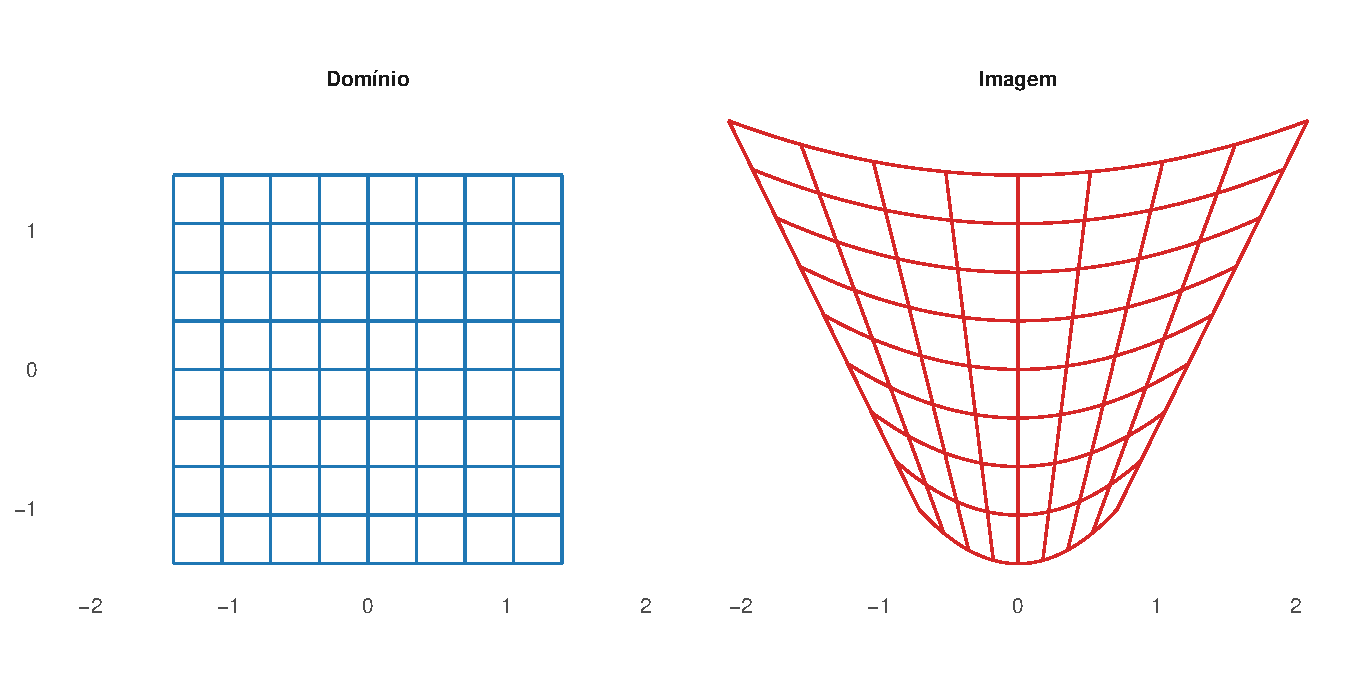
\includegraphics[keepaspectratio]{mod_1_calculo_files/figure-pdf/fig-jacobiano-alteracao-area-1.pdf}}

}

\caption{\label{fig-jacobiano-alteracao-area}Transformação de uma grade
e alteração local de área determinada pelo Jacobiano.}

\end{figure}%

Uma pequena região em torno de \(\mathbf{x}\) tem sua área multiplicada
aproximadamente por

\[
\left|
\det
\mathbf{J}_{\mathbf{g}}(\mathbf{x})
\right|.
\]

A imagem da grade apresenta expansão e contração diferentes ao longo do
domínio porque o determinante Jacobiano não é constante.

\subsection{Coordenadas polares}\label{coordenadas-polares}

Em duas dimensões, defina

\[
x_1
=
r\cos\theta
\]

e

\[
x_2
=
r\sin\theta,
\]

com

\[
r>0
\]

e

\[
0\leq\theta<2\pi.
\]

A transformação é

\[
\mathbf{g}(r,\theta)
=
\begin{bmatrix}
r\cos\theta\\
r\sin\theta
\end{bmatrix}.
\]

Sua Jacobiana é

\[
\mathbf{J}_{\mathbf{g}}(r,\theta)
=
\begin{bmatrix}
\cos\theta&-r\sin\theta\\
\sin\theta&r\cos\theta
\end{bmatrix}.
\]

O determinante é

\[
\det
\mathbf{J}_{\mathbf{g}}(r,\theta)
=
r.
\]

Portanto,

\[
dx_1\,dx_2
=
r\,dr\,d\theta.
\]

Assim,

\[
\iint_{\mathbb{R}^{2}}
h(x_1,x_2)
\,dx_1\,dx_2
=
\int_{0}^{2\pi}
\int_{0}^{\infty}
h
\left(
r\cos\theta,
r\sin\theta
\right)
r
\,dr\,d\theta,
\]

quando a função é integrável.

A parametrização polar não é uma transformação globalmente bijetiva em
todas as escolhas possíveis de domínio: a origem possui representação
angular não única e o ângulo é periódico. Para a aplicação da fórmula de
mudança de variáveis, trabalha-se em regiões adequadas de injetividade;
as fronteiras envolvidas possuem medida nula e não alteram o valor das
integrais usuais.

\subsection{Transformações
elipsoidais}\label{transformauxe7uxf5es-elipsoidais}

Considere uma matriz positiva definida

\[
\boldsymbol{\Sigma}
\in
\mathbb{R}^{p\times p}
\]

e sua raiz quadrada principal simétrica positiva definida

\[
\boldsymbol{\Sigma}^{1/2}.
\]

Considere a transformação

\[
\mathbf{x}
=
\boldsymbol{\mu}
+
\boldsymbol{\Sigma}^{1/2}\mathbf{z}.
\]

A Jacobiana é

\[
\mathbf{J}_{\mathbf{g}}(\mathbf{z})
=
\boldsymbol{\Sigma}^{1/2}.
\]

Logo,

\[
\left|
\det
\mathbf{J}_{\mathbf{g}}(\mathbf{z})
\right|
=
\det
\left(
\boldsymbol{\Sigma}^{1/2}
\right)
=
\det(\boldsymbol{\Sigma})^{1/2}.
\]

A transformação inversa é

\[
\mathbf{z}
=
\boldsymbol{\Sigma}^{-1/2}
\left(
\mathbf{x}
-
\boldsymbol{\mu}
\right),
\]

com fator

\[
\left|
\det
\mathbf{J}_{\mathbf{g}^{-1}}(\mathbf{x})
\right|
=
\det(\boldsymbol{\Sigma})^{-1/2}.
\]

Além disso,

\[
\begin{aligned}
\mathbf{z}^{\top}\mathbf{z}
&=
\left(
\mathbf{x}
-
\boldsymbol{\mu}
\right)^{\top}
\boldsymbol{\Sigma}^{-1/2}
\boldsymbol{\Sigma}^{-1/2}
\left(
\mathbf{x}
-
\boldsymbol{\mu}
\right)\\
&=
\left(
\mathbf{x}
-
\boldsymbol{\mu}
\right)^{\top}
\boldsymbol{\Sigma}^{-1}
\left(
\mathbf{x}
-
\boldsymbol{\mu}
\right).
\end{aligned}
\]

A transformação converte esferas no espaço de \(\mathbf{z}\) em
elipsoides no espaço de \(\mathbf{x}\). Essa relação será utilizada na
construção de densidades multivariadas.

\subsection{Aprofundamento: diferenciação sob o sinal de
integração}\label{aprofundamento-diferenciauxe7uxe3o-sob-o-sinal-de-integrauxe7uxe3o}

\begin{tcolorbox}[enhanced jigsaw, colback=white, breakable, bottomrule=.15mm, left=2mm, arc=.35mm, rightrule=.15mm, colframe=quarto-callout-note-color-frame, toprule=.15mm, leftrule=.75mm, opacityback=0]

\vspace{-3mm}\textbf{Leitura de aprofundamento}\vspace{3mm}

A diferenciação sob o sinal de integração é utilizada para justificar
formalmente identidades envolvendo funções de verossimilhança, vetor
escore e informação de Fisher.

Esse conteúdo é importante para desenvolvimentos inferenciais mais
formais, mas pode ser omitido em uma primeira leitura. Para a
continuidade imediata dos capítulos probabilísticos, basta reter que a
troca entre derivação e integração exige condições de regularidade e não
pode ser realizada automaticamente.

\end{tcolorbox}

Considere um conjunto mensurável

\[
\mathcal{D}
\subseteq
\mathbb{R}^{p},
\]

uma região aberta

\[
\mathcal{V}
\subseteq
\mathbb{R}^{k}
\]

e uma função

\[
h:
\mathcal{D}
\times
\mathcal{V}
\longrightarrow
\mathbb{R}.
\]

A função depende da variável de integração \(\mathbf{x}\) e do parâmetro

\[
\boldsymbol{\theta}
\in
\mathcal{V}.
\]

Defina

\[
F(\boldsymbol{\theta})
=
\int_{\mathcal{D}}
h(\mathbf{x},\boldsymbol{\theta})
\,d\mathbf{x}.
\]

A troca entre diferenciação e integração pode ser justificada pelo
Teorema da Convergência Dominada.

\begin{theorem}[Teorema da Convergência
Dominada]\protect\hypertarget{thm-convergencia-dominada}{}\label{thm-convergencia-dominada}

Considere uma sequência de funções mensuráveis

\[
g_1,g_2,\ldots
\]

definidas em \(\mathcal{D}\) e suponha que

\[
g_m(\mathbf{x})
\longrightarrow
g(\mathbf{x})
\]

para quase todo \(\mathbf{x}\in\mathcal{D}\).

Se existe uma função integrável

\[
M:
\mathcal{D}
\longrightarrow
[0,\infty)
\]

tal que

\[
|g_m(\mathbf{x})|
\leq
M(\mathbf{x})
\]

para todo \(m\) e quase todo \(\mathbf{x}\in\mathcal{D}\), então \(g\) é
integrável e

\[
\lim_{m\to\infty}
\int_{\mathcal{D}}
g_m(\mathbf{x})
\,d\mathbf{x}
=
\int_{\mathcal{D}}
g(\mathbf{x})
\,d\mathbf{x}.
\]

(Axler, 2020)

\end{theorem}

O teorema permite trocar um limite e uma integral quando todas as
funções da sequência são dominadas por uma mesma função integrável. A
diferenciação sob o sinal de integração decorre da aplicação desse
resultado aos quocientes de diferenças.

\begin{theorem}[Diferenciação sob o sinal de
integração]\protect\hypertarget{thm-diferenciacao-integral}{}\label{thm-diferenciacao-integral}

Considere um ponto

\[
\boldsymbol{\theta}_0
\in
\mathcal{V}
\]

e uma componente

\[
j
\in
\{1,\ldots,k\}.
\]

Suponha que:

\begin{enumerate}
\def\labelenumi{\arabic{enumi}.}
\item
  para todo \(\boldsymbol{\theta}\in\mathcal{V}\), a função

  \[
  \mathbf{x}
  \longmapsto
  h(\mathbf{x},\boldsymbol{\theta})
  \]

  seja mensurável e integrável em \(\mathcal{D}\);
\item
  exista \(\delta>0\) tal que

  \[
  \boldsymbol{\theta}_0
  +
  t\mathbf{e}_j
  \in
  \mathcal{V}
  \]

  para todo \(t\) com \(|t|<\delta\), em que \(\mathbf{e}_j\) é o
  \(j\)-ésimo vetor da base canônica de \(\mathbb{R}^{k}\);
\item
  para quase todo \(\mathbf{x}\in\mathcal{D}\), a função

  \[
  t
  \longmapsto
  h
  \left(
  \mathbf{x},
  \boldsymbol{\theta}_0+t\mathbf{e}_j
  \right)
  \]

  seja diferenciável em \((-\delta,\delta)\);
\item
  exista uma função integrável

  \[
  M_j:
  \mathcal{D}
  \longrightarrow
  [0,\infty)
  \]

  tal que, para quase todo

  \[
  \mathbf{x}
  \in
  \mathcal{D},
  \]

  a desigualdade

  \[
  \left|
  \frac{
  \partial
  h
  \left(
  \mathbf{x},
  \boldsymbol{\theta}_0+t\mathbf{e}_j
  \right)
  }{
  \partial\theta_j
  }
  \right|
  \leq
  M_j(\mathbf{x})
  \]

  seja válida para todo \(t\) com \(|t|<\delta\);
\item
  a função

  \[
  \mathbf{x}
  \longmapsto
  \frac{
  \partial
  h(\mathbf{x},\boldsymbol{\theta}_0)
  }{
  \partial\theta_j
  }
  \]

  seja mensurável.
\end{enumerate}

Então, \(F\) é parcialmente diferenciável em relação a \(\theta_j\) no
ponto \(\boldsymbol{\theta}_0\) e

\[
\frac{
\partial
F(\boldsymbol{\theta}_0)
}{
\partial\theta_j
}
=
\int_{\mathcal{D}}
\frac{
\partial
h(\mathbf{x},\boldsymbol{\theta}_0)
}{
\partial\theta_j
}
\,d\mathbf{x}.
\]

\end{theorem}

\begin{proof}
Considere uma sequência arbitrária de números não nulos

\[
t_1,t_2,\ldots
\]

tal que

\[
t_m
\longrightarrow
0
\]

e

\[
|t_m|<\delta.
\]

Defina o quociente de diferenças

\[
q_m(\mathbf{x})
=
\frac{
h
\left(
\mathbf{x},
\boldsymbol{\theta}_0+t_m\mathbf{e}_j
\right)
-
h
\left(
\mathbf{x},
\boldsymbol{\theta}_0
\right)
}{
t_m
}.
\]

Para quase todo \(\mathbf{x}\in\mathcal{D}\), a diferenciabilidade em
relação a \(\theta_j\) implica

\[
q_m(\mathbf{x})
\longrightarrow
\frac{
\partial
h(\mathbf{x},\boldsymbol{\theta}_0)
}{
\partial\theta_j
}.
\]

Pelo Teorema do Valor Médio aplicado à função

\[
t
\longmapsto
h
\left(
\mathbf{x},
\boldsymbol{\theta}_0+t\mathbf{e}_j
\right),
\]

existe um número \(\xi_m(\mathbf{x})\) situado entre \(0\) e \(t_m\) tal
que

\[
q_m(\mathbf{x})
=
\frac{
\partial
h
\left(
\mathbf{x},
\boldsymbol{\theta}_0+\xi_m(\mathbf{x})\mathbf{e}_j
\right)
}{
\partial\theta_j
}.
\]

Como

\[
|\xi_m(\mathbf{x})|
<
\delta,
\]

a hipótese de dominação fornece

\[
|q_m(\mathbf{x})|
\leq
M_j(\mathbf{x})
\]

para quase todo \(\mathbf{x}\in\mathcal{D}\).

O Teorema da Convergência Dominada implica

\[
\begin{aligned}
\lim_{m\to\infty}
\int_{\mathcal{D}}
q_m(\mathbf{x})
\,d\mathbf{x}
&=
\int_{\mathcal{D}}
\lim_{m\to\infty}
q_m(\mathbf{x})
\,d\mathbf{x}\\
&=
\int_{\mathcal{D}}
\frac{
\partial
h(\mathbf{x},\boldsymbol{\theta}_0)
}{
\partial\theta_j
}
\,d\mathbf{x}.
\end{aligned}
\]

Por outro lado,

\[
\begin{aligned}
\int_{\mathcal{D}}
q_m(\mathbf{x})
\,d\mathbf{x}
&=
\frac{
\displaystyle
\int_{\mathcal{D}}
h
\left(
\mathbf{x},
\boldsymbol{\theta}_0+t_m\mathbf{e}_j
\right)
\,d\mathbf{x}
-
\displaystyle
\int_{\mathcal{D}}
h
\left(
\mathbf{x},
\boldsymbol{\theta}_0
\right)
\,d\mathbf{x}
}{
t_m
}\\
&=
\frac{
F
\left(
\boldsymbol{\theta}_0+t_m\mathbf{e}_j
\right)
-
F(\boldsymbol{\theta}_0)
}{
t_m
}.
\end{aligned}
\]

Logo,

\[
\lim_{m\to\infty}
\frac{
F
\left(
\boldsymbol{\theta}_0+t_m\mathbf{e}_j
\right)
-
F(\boldsymbol{\theta}_0)
}{
t_m
}
=
\int_{\mathcal{D}}
\frac{
\partial
h(\mathbf{x},\boldsymbol{\theta}_0)
}{
\partial\theta_j
}
\,d\mathbf{x}.
\]

Como a sequência \(t_m\to0\) foi escolhida arbitrariamente, a derivada
parcial existe e satisfaz a igualdade enunciada.
\end{proof}

Quando as condições do Teorema~\ref{thm-diferenciacao-integral} são
satisfeitas para todas as componentes do parâmetro,

\[
\nabla_{\boldsymbol{\theta}}
F(\boldsymbol{\theta}_0)
=
\int_{\mathcal{D}}
\nabla_{\boldsymbol{\theta}}
h(\mathbf{x},\boldsymbol{\theta}_0)
\,d\mathbf{x}.
\]

A função dominante pode ser diferente para cada componente do gradiente,
desde que cada uma seja integrável.

O resultado pressupõe que o domínio \(\mathcal{D}\) não depende de
\(\boldsymbol{\theta}\). Quando o domínio ou a fronteira da região de
integração varia com o parâmetro, a derivação pode produzir termos
adicionais. Esse caso não será desenvolvido neste capítulo.

\begin{example}[Derivação de uma identidade de
normalização]\protect\hypertarget{exm-derivacao-normalizacao}{}\label{exm-derivacao-normalizacao}

Considere uma família de densidades

\[
f(\mathbf{x};\boldsymbol{\theta}),
\]

definida sobre um suporte comum

\[
\mathcal{D}
\]

que não depende de \(\boldsymbol{\theta}\).

Para todo \(\boldsymbol{\theta}\),

\[
\int_{\mathcal{D}}
f(\mathbf{x};\boldsymbol{\theta})
\,d\mathbf{x}
=
1.
\]

Suponha que as condições do Teorema~\ref{thm-diferenciacao-integral}
sejam satisfeitas para todas as componentes de \(\boldsymbol{\theta}\).
Então,

\[
\begin{aligned}
\mathbf{0}
&=
\nabla_{\boldsymbol{\theta}}1\\
&=
\nabla_{\boldsymbol{\theta}}
\int_{\mathcal{D}}
f(\mathbf{x};\boldsymbol{\theta})
\,d\mathbf{x}\\
&=
\int_{\mathcal{D}}
\nabla_{\boldsymbol{\theta}}
f(\mathbf{x};\boldsymbol{\theta})
\,d\mathbf{x}.
\end{aligned}
\]

Se

\[
f(\mathbf{x};\boldsymbol{\theta})
>
0
\]

para quase todo \(\mathbf{x}\in\mathcal{D}\), então

\[
\nabla_{\boldsymbol{\theta}}
f(\mathbf{x};\boldsymbol{\theta})
=
f(\mathbf{x};\boldsymbol{\theta})
\nabla_{\boldsymbol{\theta}}
\log
f(\mathbf{x};\boldsymbol{\theta}).
\]

Portanto,

\[
\int_{\mathcal{D}}
f(\mathbf{x};\boldsymbol{\theta})
\nabla_{\boldsymbol{\theta}}
\log
f(\mathbf{x};\boldsymbol{\theta})
\,d\mathbf{x}
=
\mathbf{0}.
\]

Se

\[
\boldsymbol{\mathsf X}
\]

possui densidade \(f(\mathbf{x};\boldsymbol{\theta})\), segue que

\[
E_{\boldsymbol{\theta}}
\left[
\nabla_{\boldsymbol{\theta}}
\log
f
\left(
\boldsymbol{\mathsf X};
\boldsymbol{\theta}
\right)
\right]
=
\mathbf{0}.
\]

Essa é a identidade de média nula do escore para uma observação. Sua
validade depende do suporte comum e das condições de dominação que
justificam a troca entre diferenciação e integração.

\end{example}

As integrais múltiplas, a marginalização e a mudança de variáveis
fornecem a base para o estudo das distribuições multivariadas. A parte
de aprofundamento mostrou, adicionalmente, como condições de dominação
podem justificar a diferenciação de integrais parametrizadas e
identidades utilizadas posteriormente em inferência.

Para a continuidade do livro, as ideias centrais a reter são:

\begin{itemize}
\tightlist
\item
  probabilidades são obtidas por integração da densidade conjunta;
\item
  densidades marginais são obtidas integrando as componentes que se
  deseja eliminar;
\item
  esperanças de vetores e matrizes são calculadas componente a
  componente;
\item
  mudanças de variáveis exigem o determinante absoluto da Jacobiana;
\item
  transformações afins produzem fatores de volume constantes;
\item
  transformações elipsoidais convertem geometria esférica e elipsoidal.
\end{itemize}

\section{Aprofundamento: aplicações à estimação e à
inferência}\label{aprofundamento-aplicauxe7uxf5es-uxe0-estimauxe7uxe3o-e-uxe0-inferuxeancia}

\begin{tcolorbox}[enhanced jigsaw, colback=white, breakable, bottomrule=.15mm, left=2mm, arc=.35mm, rightrule=.15mm, colframe=quarto-callout-note-color-frame, toprule=.15mm, leftrule=.75mm, opacityback=0]

\vspace{-3mm}\textbf{Leitura de aprofundamento}\vspace{3mm}

As subseções seguintes mostram como as ferramentas de cálculo
desenvolvidas neste capítulo aparecem em problemas de estimação e
inferência.

O objetivo é apresentar apenas a estrutura matemática dessas aplicações.
As propriedades probabilísticas dos estimadores, as condições de
regularidade, as distribuições assintóticas e os procedimentos
inferenciais serão desenvolvidos nos capítulos específicos do Módulo II.

Este bloco pode ser omitido em uma primeira leitura sem comprometer a
continuidade imediata do livro.

\end{tcolorbox}

As aplicações seguintes envolvem gradientes, Hessianas, expansões de
Taylor, diferenciação sob o sinal de integração e cálculo matricial.
Elas antecipam, em nível matemático, conceitos que serão retomados
posteriormente.

\subsection{Log-verossimilhança e vetor
escore}\label{log-verossimilhanuxe7a-e-vetor-escore}

Considere observações independentes

\[
\mathbf{x}_1,\ldots,\mathbf{x}_n
\]

provenientes de um mesmo modelo paramétrico com função de densidade ou
de probabilidade

\[
f(\mathbf{x};\boldsymbol{\theta}),
\]

em que

\[
\boldsymbol{\theta}
\in
\Theta
\subseteq
\mathbb{R}^{k}
\]

é o vetor de parâmetros e \(\Theta\) é o espaço paramétrico.

Nessas condições, a função de verossimilhança é

\[
L_n(\boldsymbol{\theta})
=
\prod_{i=1}^{n}
f(\mathbf{x}_i;\boldsymbol{\theta}).
\]

A log-verossimilhança é

\[
\ell_n(\boldsymbol{\theta})
=
\log
L_n(\boldsymbol{\theta})
=
\sum_{i=1}^{n}
\log
f(\mathbf{x}_i;\boldsymbol{\theta}).
\]

Como o logaritmo é estritamente crescente, maximizar \(L_n\) equivale a
maximizar \(\ell_n\).

\begin{definition}[Vetor
escore]\protect\hypertarget{def-vetor-escore}{}\label{def-vetor-escore}

O vetor escore é o gradiente da log-verossimilhança:

\[
\mathbf{s}_n(\boldsymbol{\theta})
=
\nabla_{\boldsymbol{\theta}}
\ell_n(\boldsymbol{\theta})
\in
\mathbb{R}^{k}.
\]

\end{definition}

Em coordenadas,

\[
\mathbf{s}_n(\boldsymbol{\theta})
=
\begin{bmatrix}
\dfrac{
\partial\ell_n
}{
\partial\theta_1
}\\
\vdots\\
\dfrac{
\partial\ell_n
}{
\partial\theta_k
}
\end{bmatrix}.
\]

Se um estimador de máxima verossimilhança é um ponto interior do espaço
paramétrico e a log-verossimilhança é diferenciável nesse ponto, então
deve satisfazer

\[
\mathbf{s}_n
\left(
\widehat{\boldsymbol{\theta}}
\right)
=
\mathbf{0}.
\]

Essa condição é necessária, mas pode não ser suficiente para identificar
um máximo. Também devem ser examinados:

\begin{itemize}
\tightlist
\item
  a curvatura da log-verossimilhança;
\item
  a existência e a unicidade da solução;
\item
  os limites do espaço paramétrico;
\item
  possíveis máximos na fronteira.
\end{itemize}

\subsection{Informação observada e informação de
Fisher}\label{informauxe7uxe3o-observada-e-informauxe7uxe3o-de-fisher}

\begin{definition}[Informação
observada]\protect\hypertarget{def-informacao-observada}{}\label{def-informacao-observada}

A matriz de informação observada é

\[
\mathcal{J}_n(\boldsymbol{\theta})
=
-
\nabla_{\boldsymbol{\theta}}^2
\ell_n(\boldsymbol{\theta}).
\]

\end{definition}

Se

\[
\mathbf{s}_n
\left(
\widehat{\boldsymbol{\theta}}
\right)
=
\mathbf{0}
\]

e

\[
\mathcal{J}_n
\left(
\widehat{\boldsymbol{\theta}}
\right)
\succ
\mathbf{0},
\]

então

\[
\nabla_{\boldsymbol{\theta}}^2
\ell_n
\left(
\widehat{\boldsymbol{\theta}}
\right)
\prec
\mathbf{0},
\]

e o teste da Hessiana fornece uma condição suficiente para que
\(\widehat{\boldsymbol{\theta}}\) seja um máximo local estrito da
log-verossimilhança.

Em um ponto arbitrário do espaço paramétrico, a matriz

\[
\mathcal{J}_n(\boldsymbol{\theta})
=
-
\nabla_{\boldsymbol{\theta}}^2
\ell_n(\boldsymbol{\theta})
\]

não precisa ser positiva semidefinida e pode, inclusive, ser indefinida.

Em um ponto estacionário interior que seja máximo local,

\[
\nabla_{\boldsymbol{\theta}}^2
\ell_n(\widehat{\boldsymbol{\theta}})
\preceq
\mathbf{0},
\]

de modo que

\[
\mathcal{J}_n(\widehat{\boldsymbol{\theta}})
\succeq
\mathbf{0}.
\]

A informação observada pode ser singular quando, por exemplo:

\begin{itemize}
\tightlist
\item
  há parâmetros localmente não identificados;
\item
  existem redundâncias na parametrização;
\item
  a log-verossimilhança apresenta direções localmente planas.
\end{itemize}

Máximos na fronteira exigem tratamento separado, pois as condições
usuais de ponto estacionário e o teste irrestrito da Hessiana não os
caracterizam adequadamente.

\begin{definition}[Informação de
Fisher]\protect\hypertarget{def-informacao-fisher}{}\label{def-informacao-fisher}

Suponha que o vetor escore possua segundo momento finito. A informação
de Fisher da amostra é definida por

\[
\mathcal{I}_n(\boldsymbol{\theta})
=
E_{\boldsymbol{\theta}}
\left[
\mathbf{s}_n(\boldsymbol{\theta})
\mathbf{s}_n(\boldsymbol{\theta})^{\top}
\right].
\]

(Casella; Berger, 2002)

\end{definition}

Sob condições de regularidade que permitem diferenciar a densidade sob o
sinal de integração,

\[
E_{\boldsymbol{\theta}}
\left[
\mathbf{s}_n(\boldsymbol{\theta})
\right]
=
\mathbf{0}.
\]

Sob condições adicionais que justificam a relação entre a primeira e a
segunda derivadas da log-verossimilhança,

\[
\begin{aligned}
\mathcal{I}_n(\boldsymbol{\theta})
&=
-
E_{\boldsymbol{\theta}}
\left[
\nabla_{\boldsymbol{\theta}}^2
\ell_n(\boldsymbol{\theta})
\right]\\
&=
E_{\boldsymbol{\theta}}
\left[
\mathcal{J}_n(\boldsymbol{\theta})
\right].
\end{aligned}
\]

Assim, em modelos regulares, a informação de Fisher coincide com a
esperança da informação observada. Como o escore possui esperança nula
nessas condições,

\[
\mathcal{I}_n(\boldsymbol{\theta})
=
\operatorname{Cov}_{\boldsymbol{\theta}}
\left[
\mathbf{s}_n(\boldsymbol{\theta})
\right].
\]

Essas identidades não devem ser utilizadas automaticamente. Sua validade
depende das condições de regularidade, incluindo a possibilidade de
intercambiar derivação e integração e o comportamento do suporte em
relação ao parâmetro.

\subsection{Newton--Raphson}\label{newtonraphson}

A estimação por máxima verossimilhança pode exigir a solução numérica de

\[
\mathbf{s}_n(\boldsymbol{\theta})
=
\mathbf{0}.
\]

A expansão de primeira ordem do escore em torno de um valor atual
\(\boldsymbol{\theta}^{(t)}\) é

\[
\mathbf{s}_n(\boldsymbol{\theta})
\approx
\mathbf{s}_n
\left(
\boldsymbol{\theta}^{(t)}
\right)
+
\nabla_{\boldsymbol{\theta}}^2
\ell_n
\left(
\boldsymbol{\theta}^{(t)}
\right)
\left(
\boldsymbol{\theta}
-
\boldsymbol{\theta}^{(t)}
\right).
\]

Igualando a aproximação a zero,

\[
\begin{aligned}
\boldsymbol{\theta}^{(t+1)}
&=
\boldsymbol{\theta}^{(t)}
-
\left[
\nabla_{\boldsymbol{\theta}}^2
\ell_n
\left(
\boldsymbol{\theta}^{(t)}
\right)
\right]^{-1}
\mathbf{s}_n
\left(
\boldsymbol{\theta}^{(t)}
\right)\\
&=
\boldsymbol{\theta}^{(t)}
+
\mathcal{J}_n
\left(
\boldsymbol{\theta}^{(t)}
\right)^{-1}
\mathbf{s}_n
\left(
\boldsymbol{\theta}^{(t)}
\right).
\end{aligned}
\]

Na implementação, a atualização deve ser obtida pela solução do sistema

\[
\mathcal{J}_n
\left(
\boldsymbol{\theta}^{(t)}
\right)
\mathbf{d}^{(t)}
=
\mathbf{s}_n
\left(
\boldsymbol{\theta}^{(t)}
\right),
\]

seguida de

\[
\boldsymbol{\theta}^{(t+1)}
=
\boldsymbol{\theta}^{(t)}
+
\mathbf{d}^{(t)}.
\]

Isso evita calcular explicitamente a inversa da informação observada.

Essa é a aplicação do método de Newton à equação

\[
\mathbf{s}_n(\boldsymbol{\theta})
=
\mathbf{0}.
\]

Quando

\[
\mathcal{J}_n
\left(
\boldsymbol{\theta}^{(t)}
\right)
\succ
\mathbf{0},
\]

a direção

\[
\mathbf{d}^{(t)}
=
\mathcal{J}_n
\left(
\boldsymbol{\theta}^{(t)}
\right)^{-1}
\mathbf{s}_n
\left(
\boldsymbol{\theta}^{(t)}
\right)
\]

é uma direção local de aumento da log-verossimilhança, pois

\[
\mathbf{s}_n
\left(
\boldsymbol{\theta}^{(t)}
\right)^{\top}
\mathbf{d}^{(t)}
>
0
\]

quando o escore é não nulo.

Ainda assim, um passo completo pode não aumentar a log-verossimilhança
quando o ponto atual está distante da solução. Em aplicações numéricas,
podem ser utilizados controles do comprimento da etapa.

\subsection{Método do escore de
Fisher}\label{muxe9todo-do-escore-de-fisher}

O método do escore de Fisher substitui a informação observada

\[
\mathcal{J}_n(\boldsymbol{\theta})
\]

pela informação de Fisher

\[
\mathcal{I}_n(\boldsymbol{\theta}).
\]

Sob as condições de regularidade para as quais

\[
\mathcal{I}_n(\boldsymbol{\theta})
=
E_{\boldsymbol{\theta}}
\left[
\mathcal{J}_n(\boldsymbol{\theta})
\right],
\]

essa substituição pode ser interpretada como a troca da curvatura
observada pela curvatura esperada da log-verossimilhança.

Quando

\[
\mathcal{I}_n
\left(
\boldsymbol{\theta}^{(t)}
\right)
\]

é invertível, a direção \(\mathbf{d}^{(t)}\) é obtida pela solução de

\[
\mathcal{I}_n
\left(
\boldsymbol{\theta}^{(t)}
\right)
\mathbf{d}^{(t)}
=
\mathbf{s}_n
\left(
\boldsymbol{\theta}^{(t)}
\right),
\]

seguida da atualização

\[
\boldsymbol{\theta}^{(t+1)}
=
\boldsymbol{\theta}^{(t)}
+
\mathbf{d}^{(t)}.
\]

Assim, Newton--Raphson utiliza

\[
\mathcal{J}_n(\boldsymbol{\theta}),
\]

enquanto o método do escore de Fisher utiliza

\[
\mathcal{I}_n(\boldsymbol{\theta}).
\]

Quando a identidade de informação é válida, a primeira representa a
curvatura observada e a segunda sua correspondente curvatura esperada.

As atualizações coincidem quando as duas matrizes são iguais no ponto
considerado ou, mais geralmente, quando produzem a mesma solução para a
equação que determina a direção da etapa.

\subsection{Expansão local de uma raiz do
escore}\label{expansuxe3o-local-de-uma-raiz-do-escore}

Suponha que um estimador

\[
\widehat{\boldsymbol{\theta}}
\]

satisfaça a equação

\[
\mathbf{s}_n
\left(
\widehat{\boldsymbol{\theta}}
\right)
=
\mathbf{0}.
\]

Expandindo o escore em torno do parâmetro verdadeiro
\(\boldsymbol{\theta}_0\),

\[
\begin{aligned}
\mathbf{0}
&=
\mathbf{s}_n
\left(
\widehat{\boldsymbol{\theta}}
\right)\\
&\approx
\mathbf{s}_n
\left(
\boldsymbol{\theta}_0
\right)
+
\nabla_{\boldsymbol{\theta}}^2
\ell_n
\left(
\boldsymbol{\theta}_0
\right)
\left(
\widehat{\boldsymbol{\theta}}
-
\boldsymbol{\theta}_0
\right).
\end{aligned}
\]

Como

\[
\nabla_{\boldsymbol{\theta}}^2
\ell_n
\left(
\boldsymbol{\theta}_0
\right)
=
-
\mathcal{J}_n
\left(
\boldsymbol{\theta}_0
\right),
\]

obtém-se a aproximação

\[
\widehat{\boldsymbol{\theta}}
-
\boldsymbol{\theta}_0
\approx
\mathcal{J}_n
\left(
\boldsymbol{\theta}_0
\right)^{-1}
\mathbf{s}_n
\left(
\boldsymbol{\theta}_0
\right).
\]

Essa expressão é uma aproximação local de primeira ordem. A obtenção de
uma representação assintótica rigorosa exige controlar o termo restante
da expansão e substituir a informação observada por um limite
apropriado.

Essa relação mostra que o erro do estimador pode ser aproximado pelo
produto entre:

\begin{itemize}
\tightlist
\item
  a inversa da curvatura da log-verossimilhança;
\item
  o escore calculado no parâmetro verdadeiro.
\end{itemize}

A obtenção de uma distribuição assintótica exige resultados
probabilísticos adicionais sobre consistência, convergência da
informação e distribuição limite do escore.

\subsection{Método delta}\label{muxe9todo-delta}

O método delta utiliza a aproximação de Taylor para obter a distribuição
aproximada de uma transformação de um estimador.

\begin{theorem}[Método delta
multivariado]\protect\hypertarget{thm-metodo-delta}{}\label{thm-metodo-delta}

Suponha que

\[
\sqrt{n}
\left(
\widehat{\boldsymbol{\theta}}
-
\boldsymbol{\theta}
\right)
\overset{d}{\longrightarrow}
N_k
\left(
\mathbf{0},
\boldsymbol{\Xi}
\right),
\]

em que

\[
\boldsymbol{\Xi}
\in
\mathbb{R}^{k\times k}.
\]

Considere uma função

\[
\mathbf{g}:
\mathbb{R}^{k}
\longrightarrow
\mathbb{R}^{q}
\]

diferenciável no ponto

\[
\boldsymbol{\theta}.
\]

Então,

\[
\sqrt{n}
\left[
\mathbf{g}
\left(
\widehat{\boldsymbol{\theta}}
\right)
-
\mathbf{g}
\left(
\boldsymbol{\theta}
\right)
\right]
\overset{d}{\longrightarrow}
N_q
\left(
\mathbf{0},
\mathbf{J}_{\mathbf{g}}(\boldsymbol{\theta})
\boldsymbol{\Xi}
\mathbf{J}_{\mathbf{g}}(\boldsymbol{\theta})^{\top}
\right).
\]

(Vaart, 1998)

\end{theorem}

A demonstração formal utiliza a aproximação de Taylor de primeira ordem
juntamente com resultados probabilísticos sobre convergência em
distribuição. Esses resultados serão desenvolvidos no módulo
inferencial; neste capítulo interessa principalmente a origem
diferencial da matriz

\[
\mathbf{J}_{\mathbf{g}}(\boldsymbol{\theta})
\boldsymbol{\Xi}
\mathbf{J}_{\mathbf{g}}(\boldsymbol{\theta})^{\top}.
\]

A aproximação de primeira ordem é

\[
\mathbf{g}
\left(
\widehat{\boldsymbol{\theta}}
\right)
-
\mathbf{g}
\left(
\boldsymbol{\theta}
\right)
\approx
\mathbf{J}_{\mathbf{g}}(\boldsymbol{\theta})
\left(
\widehat{\boldsymbol{\theta}}
-
\boldsymbol{\theta}
\right).
\]

A matriz

\[
\mathbf{V}_{\mathbf{g}}
=
\mathbf{J}_{\mathbf{g}}(\boldsymbol{\theta})
\boldsymbol{\Xi}
\mathbf{J}_{\mathbf{g}}(\boldsymbol{\theta})^{\top}
\]

é a matriz de covariâncias da distribuição limite de

\[
\sqrt{n}
\left[
\mathbf{g}
\left(
\widehat{\boldsymbol{\theta}}
\right)
-
\mathbf{g}
\left(
\boldsymbol{\theta}
\right)
\right].
\]

Por isso, denomina-se

\[
\frac1n
\mathbf{V}_{\mathbf{g}}
\]

matriz de covariâncias assintótica de

\[
\mathbf{g}
\left(
\widehat{\boldsymbol{\theta}}
\right).
\]

Em aplicações, é comum utilizá-la como aproximação da matriz de
covariâncias do estimador para amostras grandes. A convergência em
distribuição, isoladamente, não garante convergência dos segundos
momentos; essa interpretação requer condições adicionais de
regularidade.

Para uma função escalar

\[
g:
\mathbb{R}^{k}
\longrightarrow
\mathbb{R},
\]

a variância assintótica é

\[
\frac1n
\nabla_{\boldsymbol{\theta}}g(\boldsymbol{\theta})^{\top}
\boldsymbol{\Xi}
\nabla_{\boldsymbol{\theta}}g(\boldsymbol{\theta}).
\]

\begin{example}[Método delta para uma
razão]\protect\hypertarget{exm-metodo-delta-razao}{}\label{exm-metodo-delta-razao}

Considere

\[
\boldsymbol{\theta}
=
\begin{bmatrix}
\theta_1\\
\theta_2
\end{bmatrix},
\qquad
\theta_2\neq0,
\]

e

\[
g(\boldsymbol{\theta})
=
\frac{\theta_1}{\theta_2}.
\]

O gradiente é

\[
\nabla_{\boldsymbol{\theta}}g
=
\begin{bmatrix}
\dfrac{1}{\theta_2}\\[6pt]
-\dfrac{\theta_1}{\theta_2^2}
\end{bmatrix}.
\]

Se

\[
\sqrt{n}
\left(
\widehat{\boldsymbol{\theta}}
-
\boldsymbol{\theta}
\right)
\overset{d}{\longrightarrow}
N_2
\left(
\mathbf{0},
\boldsymbol{\Xi}
\right),
\]

então

\[
\sqrt{n}
\left(
\frac{
\widehat{\theta}_1
}{
\widehat{\theta}_2
}
-
\frac{
\theta_1
}{
\theta_2
}
\right)
\]

converge em distribuição para uma normal com variância assintótica

\[
\nabla_{\boldsymbol{\theta}}g(\boldsymbol{\theta})^{\top}
\boldsymbol{\Xi}
\nabla_{\boldsymbol{\theta}}g(\boldsymbol{\theta}).
\]

\end{example}

\begin{example}[Estimação de um vetor de
médias]\protect\hypertarget{exm-estimacao-vetor-medias}{}\label{exm-estimacao-vetor-medias}

Considere observações

\[
\mathbf{x}_1,\ldots,\mathbf{x}_n
\in
\mathbb{R}^{p}
\]

e uma matriz positiva definida conhecida

\[
\boldsymbol{\Sigma}.
\]

Considere o critério

\[
Q(\boldsymbol{\mu})
=
\sum_{i=1}^{n}
\left(
\mathbf{x}_i
-
\boldsymbol{\mu}
\right)^{\top}
\boldsymbol{\Sigma}^{-1}
\left(
\mathbf{x}_i
-
\boldsymbol{\mu}
\right).
\]

O gradiente é

\[
\nabla_{\boldsymbol{\mu}}Q
=
-2
\boldsymbol{\Sigma}^{-1}
\sum_{i=1}^{n}
\left(
\mathbf{x}_i
-
\boldsymbol{\mu}
\right).
\]

A condição de primeira ordem é

\[
\sum_{i=1}^{n}
\left(
\mathbf{x}_i
-
\boldsymbol{\mu}
\right)
=
\mathbf{0}.
\]

Logo,

\[
\widehat{\boldsymbol{\mu}}
=
\frac1n
\sum_{i=1}^{n}
\mathbf{x}_i.
\]

A Hessiana é

\[
\nabla_{\boldsymbol{\mu}}^2Q
=
2n
\boldsymbol{\Sigma}^{-1}
\succ
\mathbf{0}.
\]

Portanto, o vetor de médias amostrais é o único minimizador do critério.

\end{example}

\begin{example}[Critério do modelo linear
multivariado]\protect\hypertarget{exm-criterio-modelo-linear-multivariado}{}\label{exm-criterio-modelo-linear-multivariado}

Considere

\[
\mathbf{Y}
=
\mathbf{X}\mathbf{B}
+
\boldsymbol{\mathcal E},
\]

com

\[
\mathbf{Y}
\in
\mathbb{R}^{n\times p},
\qquad
\mathbf{X}
\in
\mathbb{R}^{n\times k},
\qquad
\mathbf{B}
\in
\mathbb{R}^{k\times p}.
\]

Para

\[
\boldsymbol{\Sigma}\succ\mathbf{0},
\]

considere o critério

\[
\begin{aligned}
Q(\mathbf{B},\boldsymbol{\Sigma})
&=
\frac{n}{2}
\log\det(\boldsymbol{\Sigma})\\
&\quad+
\frac12
\operatorname{tr}
\left[
\boldsymbol{\Sigma}^{-1}
\left(
\mathbf{Y}
-
\mathbf{X}\mathbf{B}
\right)^{\top}
\left(
\mathbf{Y}
-
\mathbf{X}\mathbf{B}
\right)
\right].
\end{aligned}
\]

Para \(\boldsymbol{\Sigma}\) fixada,

\[
\nabla_{\mathbf{B}}Q
=
-
\mathbf{X}^{\top}
\left(
\mathbf{Y}
-
\mathbf{X}\mathbf{B}
\right)
\boldsymbol{\Sigma}^{-1}.
\]

A condição de primeira ordem é

\[
\mathbf{X}^{\top}
\left(
\mathbf{Y}
-
\mathbf{X}\mathbf{B}
\right)
=
\mathbf{0}.
\]

Se \(\mathbf{X}\) possui posto coluna completo,

\[
\widehat{\mathbf{B}}
=
\left(
\mathbf{X}^{\top}\mathbf{X}
\right)^{-1}
\mathbf{X}^{\top}\mathbf{Y}.
\]

Observe que, para \(\boldsymbol{\Sigma}\) fixa e positiva definida, o
minimizador em relação a \(\mathbf{B}\) não depende de
\(\boldsymbol{\Sigma}\). Isso decorre do fato de que
\(\boldsymbol{\Sigma}^{-1}\) é invertível e desaparece da condição de
primeira ordem.

Defina a matriz de Gram dos resíduos

\[
\mathbf{G}_{\mathcal E}
=
\left(
\mathbf{Y}
-
\mathbf{X}\widehat{\mathbf{B}}
\right)^{\top}
\left(
\mathbf{Y}
-
\mathbf{X}\widehat{\mathbf{B}}
\right).
\]

Para \(\mathbf{B}=\widehat{\mathbf{B}}\), o critério em relação a
\(\boldsymbol{\Sigma}\) é

\[
Q(\boldsymbol{\Sigma})
=
\frac{n}{2}
\log\det(\boldsymbol{\Sigma})
+
\frac12
\operatorname{tr}
\left(
\boldsymbol{\Sigma}^{-1}\mathbf{G}_{\mathcal E}
\right).
\]

Se

\[
\mathbf{G}_{\mathcal E}\succ\mathbf{0},
\]

o minimizador interior é

\[
\widehat{\boldsymbol{\Sigma}}
=
\frac1n
\mathbf{G}_{\mathcal E}.
\]

A condição

\[
\mathbf{G}_{\mathcal E}\succ\mathbf{0}
\]

exige que a matriz residual possua posto coluna completo.

Se \(\mathbf{X}\) possui posto coluna completo \(k\), a matriz residual
pode ser escrita como

\[
\mathbf{Y}
-
\mathbf{X}\widehat{\mathbf{B}}
=
\left(
\mathbf{I}_n
-
\mathbf{P}_{\mathbf{X}}
\right)
\mathbf{Y},
\]

em que

\[
\operatorname{posto}
\left(
\mathbf{I}_n
-
\mathbf{P}_{\mathbf{X}}
\right)
=
n-k.
\]

Consequentemente,

\[
\operatorname{posto}
\left(
\mathbf{Y}
-
\mathbf{X}\widehat{\mathbf{B}}
\right)
\leq
\min(p,n-k).
\]

Assim, uma condição necessária para

\[
\mathbf{G}_{\mathcal E}\succ\mathbf{0}
\]

é

\[
n-k
\geq
p.
\]

Quando \(\mathbf{G}_{\mathcal E}\) é singular, o critério é ilimitado
inferiormente no cone das matrizes positivas definidas. Em particular,
pode-se fazer um autovalor de \(\boldsymbol{\Sigma}\) tender a zero em
uma direção pertencente ao núcleo de \(\mathbf{G}_{\mathcal E}\) sem
produzir aumento compensatório no termo de traço.

Aqui o modelo foi utilizado apenas como uma aplicação conjunta de
gradientes matriciais, log-determinante e diferenciação de funções
envolvendo matrizes inversas.

A interpretação probabilística do critério, as propriedades dos
estimadores, suas distribuições e a formulação de hipóteses serão
desenvolvidas posteriormente nos capítulos de estimação, modelo linear
multivariado e inferência.

\end{example}

O bloco de aprofundamento mostrou como as ferramentas de cálculo deste
capítulo aparecem em problemas de estimação e inferência:

\begin{longtable}[]{@{}ll@{}}
\caption{Relações entre as ferramentas de cálculo e suas aplicações
estatísticas.}\label{tbl-calculo-inferencia}\tabularnewline
\toprule\noalign{}
Ferramenta matemática & Aplicação estatística \\
\midrule\noalign{}
\endfirsthead
\toprule\noalign{}
Ferramenta matemática & Aplicação estatística \\
\midrule\noalign{}
\endhead
\bottomrule\noalign{}
\endlastfoot
Gradiente & Vetor escore \\
Hessiana & Informação observada \\
Esperança da curvatura & Informação de Fisher \\
Expansão de Taylor & Aproximações locais e método delta \\
Cálculo matricial & Estimação de parâmetros vetoriais e matriciais \\
\end{longtable}

Essas relações devem ser entendidas neste capítulo como aplicações das
ferramentas matemáticas. Sua interpretação estatística completa será
retomada no Módulo II.

\section{Síntese do capítulo}\label{suxedntese-do-capuxedtulo-6}

O capítulo reuniu as ferramentas de cálculo necessárias para estudar
funções de vetores e matrizes e para formular problemas posteriores da
Estatística Multivariada.

No cálculo diferencial, o gradiente representa a variação de primeira
ordem de uma função escalar, a Jacobiana representa a transformação
linear local de uma função vetorial e a Hessiana descreve sua curvatura.
Essas estruturas sustentam aproximações de Taylor e condições de
otimalidade.

A otimização utiliza essas derivadas de formas diferentes. Em problemas
sem restrições, pontos estacionários e a definitude da Hessiana permitem
caracterizar soluções locais, enquanto a convexidade fornece resultados
globais. Em problemas com restrições de igualdade, os multiplicadores de
Lagrange incorporam a geometria do conjunto viável. As funções de
resíduos mostram como essas ferramentas conduzem às equações normais e
aos problemas de mínimos quadrados.

No cálculo matricial, os diferenciais e as identidades de traço permitem
trabalhar diretamente com parâmetros matriciais. Derivadas de inversas,
determinantes e log-determinantes serão utilizadas em critérios que
envolvem matrizes de covariâncias. A vetorização e o produto de
Kronecker fornecem uma representação vetorial para transformações entre
matrizes.

O cálculo integral completa essa estrutura ao permitir a obtenção de
probabilidades, expectativas e densidades marginais. O Teorema da
Mudança de Variáveis mostra como o determinante Jacobiano modifica
elementos de volume e densidades sob transformações. Transformações
afins e elipsoidais conectam essa ideia às formas quadráticas e às
matrizes positivas definidas.

As principais relações estabelecidas no capítulo podem ser resumidas da
seguinte forma:

\begin{longtable}[]{@{}
  >{\raggedright\arraybackslash}p{(\linewidth - 2\tabcolsep) * \real{0.5000}}
  >{\raggedright\arraybackslash}p{(\linewidth - 2\tabcolsep) * \real{0.5000}}@{}}
\caption{Relações entre as ferramentas do cálculo e seus usos
posteriores.}\label{tbl-relacoes-calculo}\tabularnewline
\toprule\noalign{}
\begin{minipage}[b]{\linewidth}\raggedright
Estrutura matemática
\end{minipage} & \begin{minipage}[b]{\linewidth}\raggedright
Papel nos capítulos seguintes
\end{minipage} \\
\midrule\noalign{}
\endfirsthead
\toprule\noalign{}
\begin{minipage}[b]{\linewidth}\raggedright
Estrutura matemática
\end{minipage} & \begin{minipage}[b]{\linewidth}\raggedright
Papel nos capítulos seguintes
\end{minipage} \\
\midrule\noalign{}
\endhead
\bottomrule\noalign{}
\endlastfoot
Derivadas & Aproximação local e otimização \\
Diferenciais matriciais & Manipulação e estimação de parâmetros
matriciais \\
Integração e Jacobianos & Construção e transformação de distribuições
multivariadas \\
\end{longtable}

A Tabela~\ref{tbl-identidades-calculo} reúne algumas das identidades de
uso recorrente.

\begin{longtable}[]{@{}
  >{\raggedright\arraybackslash}p{(\linewidth - 2\tabcolsep) * \real{0.5000}}
  >{\raggedright\arraybackslash}p{(\linewidth - 2\tabcolsep) * \real{0.5000}}@{}}
\caption{Identidades selecionadas de cálculo vetorial e
matricial.}\label{tbl-identidades-calculo}\tabularnewline
\toprule\noalign{}
\begin{minipage}[b]{\linewidth}\raggedright
Função ou transformação
\end{minipage} & \begin{minipage}[b]{\linewidth}\raggedright
Derivada ou diferencial
\end{minipage} \\
\midrule\noalign{}
\endfirsthead
\toprule\noalign{}
\begin{minipage}[b]{\linewidth}\raggedright
Função ou transformação
\end{minipage} & \begin{minipage}[b]{\linewidth}\raggedright
Derivada ou diferencial
\end{minipage} \\
\midrule\noalign{}
\endhead
\bottomrule\noalign{}
\endlastfoot
\(f(\mathbf{x})=\mathbf{a}^{\top}\mathbf{x}\) &
\(\nabla_{\mathbf{x}}f=\mathbf{a}\) \\
\(f(\mathbf{x})=\mathbf{x}^{\top}\mathbf{A}\mathbf{x}\) &
\(\nabla_{\mathbf{x}}f=(\mathbf{A}+\mathbf{A}^{\top})\mathbf{x}\) \\
\(f(\mathbf{x})=\|\mathbf{b}-\mathbf{A}\mathbf{x}\|^2\) &
\(\nabla_{\mathbf{x}}f=-2\mathbf{A}^{\top}(\mathbf{b}-\mathbf{A}\mathbf{x})\) \\
\(\phi(\mathbf{X})=\operatorname{tr}(\mathbf{A}^{\top}\mathbf{X})\) &
\(\nabla_{\mathbf{X}}\phi=\mathbf{A}\) \\
\(\phi(\mathbf{X})=\|\mathbf{X}\|_F^2\) &
\(\nabla_{\mathbf{X}}\phi=2\mathbf{X}\) \\
\(\mathbf{X}\mapsto\mathbf{X}^{-1}\) &
\(d(\mathbf{X}^{-1})=-\mathbf{X}^{-1}(d\mathbf{X})\mathbf{X}^{-1}\) \\
\(\phi(\mathbf{X})=\log\det(\mathbf{X})\), \(\mathbf{X}\succ\mathbf{0}\)
& \(d\phi=\operatorname{tr}(\mathbf{X}^{-1}d\mathbf{X})\) \\
\(\mathbf{Y}=\mathbf{A}\mathbf{X}\boldsymbol{\Gamma}\) &
\(\operatorname{vec}(\mathbf{Y})=(\boldsymbol{\Gamma}^{\top}\otimes\mathbf{A})\operatorname{vec}(\mathbf{X})\) \\
\end{longtable}

Os blocos de aprofundamento desenvolveram ferramentas que não são
necessárias para uma primeira leitura do capítulo, entre elas derivadas
vetorizadas e parametrização de matrizes simétricas, diferenciação sob o
sinal de integração e aplicações do cálculo à estimação e à inferência.
Esses resultados poderão ser retomados quando forem necessários nos
capítulos posteriores.

Ao final deste capítulo, o estudante deverá ser capaz de:

\begin{itemize}
\tightlist
\item
  distinguir gradiente, Jacobiana, Hessiana e gradiente matricial;
\item
  interpretar derivadas como aproximações locais;
\item
  utilizar Taylor e a Hessiana em problemas de otimização;
\item
  formular condições de primeira ordem com e sem restrições;
\item
  derivar critérios quadráticos e equações normais;
\item
  utilizar diferenciais e identidades de traço em funções matriciais;
\item
  diferenciar expressões envolvendo inversas, determinantes e
  log-determinantes;
\item
  utilizar \(\operatorname{vec}\), produto de Kronecker e sua identidade
  de vetorização;
\item
  calcular probabilidades, expectativas e densidades marginais por
  integração;
\item
  aplicar mudanças de variáveis e interpretar o determinante Jacobiano.
\end{itemize}

O Capítulo 7 encerra o \textbf{Módulo I --- Fundamentos Matemáticos e
Geométricos da Análise Multivariada}.

Antes do início do Módulo II, os \textbf{Exercícios de fixação do Módulo
I} retomam de forma integrada os principais conceitos desenvolvidos ao
longo dos sete capítulos. Os exercícios articulam representação
matricial dos dados, projeções, transformações lineares, formas
quadráticas, autovalores e autovetores, SVD, pseudoinversa e cálculo
vetorial e matricial em problemas que serão utilizados posteriormente na
Estatística Multivariada.

O capítulo seguinte inicia o \textbf{Módulo II --- Fundamentos
Probabilísticos e Inferenciais da Análise Multivariada} com o estudo das
matrizes de covariâncias e correlações. Gradientes, formas quadráticas,
transformações lineares, integrais, projeções e produtos matriciais
fornecerão as ferramentas matemáticas para descrever a variabilidade
conjunta de vetores aleatórios e sustentar os desenvolvimentos
probabilísticos e inferenciais posteriores.

\chapter*{Exercícios de fixação do Módulo
I}\label{exercuxedcios-de-fixauxe7uxe3o-do-muxf3dulo-i}
\addcontentsline{toc}{chapter}{Exercícios de fixação do Módulo I}

\markboth{Exercícios de fixação do Módulo I}{Exercícios de fixação do
Módulo I}

Os exercícios deste módulo retomam os fundamentos matemáticos
desenvolvidos nos capítulos anteriores e os utilizam em problemas que
reaparecerão ao longo da Estatística Multivariada.

A lista está dividida em duas partes. Na primeira, os problemas devem
ser resolvidos sem auxílio computacional e enfatizam conceitos,
propriedades e operações com vetores e matrizes, bem como suas
interpretações algébricas e geométricas. As matrizes foram escolhidas
para permitir resultados exatos e favorecer a compreensão das relações
entre Álgebra Linear, Geometria e Cálculo.

Na segunda parte, o \texttt{R} ou \texttt{Python} será utilizado para
estender essas mesmas ideias a matrizes de maior dimensão e a conjuntos
de dados. O objetivo não é substituir os cálculos matriciais por funções
prontas, mas utilizar a computação para aplicar e verificar propriedades
estudadas no Módulo I.

\textbf{Diretrizes gerais.} A consulta aos capítulos faz parte da
atividade. Os resultados já estabelecidos no Módulo I (definições,
teoremas, proposições, propriedades, identidades e decomposições) podem
e devem ser utilizados diretamente, sem necessidade de nova
demonstração, salvo quando isso for solicitado explicitamente.

Ao utilizar um resultado, identifique o resultado empregado e verifique
se suas condições são satisfeitas no problema considerado. Não basta
reproduzir uma fórmula. Quando uma conclusão depender de propriedades
como simetria, ortogonalidade, independência linear, posto,
invertibilidade, definição positiva ou outras condições específicas,
essas condições devem ser verificadas ou justificadas.

As questões foram elaboradas para exigir a escolha e a articulação dos
resultados adequados. Por isso, algumas fórmulas não são fornecidas no
enunciado e devem ser localizadas nos capítulos.

\section*{Parte I --- Exercícios sem uso de
computador}\label{parte-i-exercuxedcios-sem-uso-de-computador}
\addcontentsline{toc}{section}{Parte I --- Exercícios sem uso de
computador}

\markright{Parte I --- Exercícios sem uso de computador}

\begin{exercise}[Transformação de variáveis em uma matriz de
dados]\protect\hypertarget{exr-fix-m1-transformacao-dados}{}\label{exr-fix-m1-transformacao-dados}

Considere a matriz de dados

\[
\mathbf X=
\begin{bmatrix}
2&1&0\\
1&3&1\\
0&2&2\\
3&0&1
\end{bmatrix},
\]

em que as linhas representam quatro observações e as colunas representam
três variáveis.

Considere também a transformação

\[
\mathbf A=
\begin{bmatrix}
1&1&0\\
0&1&-1
\end{bmatrix}.
\]

\begin{enumerate}
\def\labelenumi{\arabic{enumi}.}
\item
  Escreva, para uma observação genérica

  \[
  \mathbf x=
  \begin{bmatrix}
  x_1\\
  x_2\\
  x_3
  \end{bmatrix},
  \]

  as duas componentes de

  \[
  \mathbf y=\mathbf A\mathbf x.
  \]
\item
  Interprete cada nova componente como uma combinação linear das
  variáveis originais.
\item
  Determine a matriz de dados transformada utilizando

  \[
  \mathbf Y
  =
  \mathbf X\mathbf A^\top.
  \]
\item
  Indique as dimensões de \(\mathbf X\), \(\mathbf A\) e \(\mathbf Y\) e
  explique por que a transformação reduziu o número de variáveis de três
  para duas.
\item
  Determine o posto de \(\mathbf A\).
\item
  Determine a dimensão de \(\mathcal N(\mathbf A)\) e explique o
  significado desse resultado em termos de perda de informação.
\item
  Sabendo apenas \(\mathbf y=\mathbf A\mathbf x\), discuta se é possível
  recuperar unicamente o vetor original \(\mathbf x\).
\end{enumerate}

\end{exercise}

\begin{exercise}[Centralização como
projeção]\protect\hypertarget{exr-fix-m1-centralizacao}{}\label{exr-fix-m1-centralizacao}

Considere \(n=4\) e defina

\[
\mathbf H_4
=
\mathbf I_4
-
\frac14
\mathbf 1_4\mathbf 1_4^\top.
\]

\begin{enumerate}
\def\labelenumi{\arabic{enumi}.}
\item
  Escreva explicitamente a matriz \(\mathbf H_4\).
\item
  Verifique que

  \[
  \mathbf H_4^\top
  =
  \mathbf H_4
  \]

  e

  \[
  \mathbf H_4^2
  =
  \mathbf H_4.
  \]
\item
  Mostre que

  \[
  \mathbf H_4\mathbf1_4
  =
  \mathbf0.
  \]
\item
  Aplique \(\mathbf H_4\) à matriz \(\mathbf X\) do
  Exercício~\ref{exr-fix-m1-transformacao-dados}:

  \[
  \mathbf X_c
  =
  \mathbf H_4\mathbf X.
  \]
\item
  Verifique diretamente que

  \[
  \mathbf1_4^\top\mathbf X_c
  =
  \mathbf0^\top.
  \]
\item
  Interprete a igualdade anterior em termos das médias das variáveis.
\end{enumerate}

\end{exercise}

\begin{exercise}[Centralização e reescalonamento das
variáveis]\protect\hypertarget{exr-fix-m1-escalonamento}{}\label{exr-fix-m1-escalonamento}

Considere uma matriz de dados

\[
\mathbf X
\in
\mathbb R^{n\times3}
\]

e a matriz diagonal

\[
\mathbf D=
\begin{bmatrix}
2&0&0\\
0&1&0\\
0&0&4
\end{bmatrix}.
\]

\begin{enumerate}
\def\labelenumi{\arabic{enumi}.}
\item
  Determine \(\mathbf D^{-1}\).
\item
  Considere inicialmente uma matriz já centralizada \(\mathbf X_c\) e
  defina

  \[
  \mathbf Z
  =
  \mathbf X_c\mathbf D^{-1}.
  \]

  Explique o efeito dessa transformação sobre cada uma das três
  variáveis.
\item
  Explique por que \(\mathbf D^{-1}\) atua à direita da matriz de dados.
\item
  Compare essa operação com a centralização

  \[
  \mathbf X_c
  =
  \mathbf H_n\mathbf X,
  \]

  explicando por que \(\mathbf H_n\) atua à esquerda enquanto
  \(\mathbf D^{-1}\) atua à direita.
\item
  Escreva, em uma única expressão, a transformação que primeiro
  centraliza \(\mathbf X\) e depois reescala suas variáveis.
\item
  A centralização e o reescalonamento atuam no mesmo espaço? Justifique
  utilizando as dimensões de \(\mathbf H_n\) e \(\mathbf D^{-1}\).
\end{enumerate}

\end{exercise}

\begin{exercise}[Duas matrizes de Gram para os mesmos
dados]\protect\hypertarget{exr-fix-m1-gram}{}\label{exr-fix-m1-gram}

Considere a matriz centralizada

\[
\mathbf X_c=
\begin{bmatrix}
1&0\\
-1&0\\
0&2\\
0&-2
\end{bmatrix}.
\]

\begin{enumerate}
\def\labelenumi{\arabic{enumi}.}
\item
  Calcule

  \[
  \mathbf G_V
  =
  \mathbf X_c^\top\mathbf X_c
  \]

  e

  \[
  \mathbf G_O
  =
  \mathbf X_c\mathbf X_c^\top.
  \]
\item
  Indique as dimensões das duas matrizes.
\item
  Qual das duas matrizes contém os produtos internos entre as colunas de
  \(\mathbf X_c\)?
\item
  Qual contém os produtos internos entre as linhas de \(\mathbf X_c\)?
\item
  Determine o posto das duas matrizes.
\item
  Determine os autovalores positivos de cada matriz.
\item
  Verifique que os autovalores positivos coincidem.
\item
  Relacione esse resultado à construção da SVD de uma matriz retangular.
\end{enumerate}

\end{exercise}

\begin{exercise}[Projeção, ajuste e
resíduos]\protect\hypertarget{exr-fix-m1-projecao-residuos}{}\label{exr-fix-m1-projecao-residuos}

Considere

\[
\mathbf X=
\begin{bmatrix}
1&0\\
1&1\\
1&2
\end{bmatrix},
\qquad
\mathbf y=
\begin{bmatrix}
1\\
2\\
2
\end{bmatrix}.
\]

\begin{enumerate}
\def\labelenumi{\arabic{enumi}.}
\item
  Verifique que as colunas de \(\mathbf X\) são linearmente
  independentes.
\item
  Determine

  \[
  \mathbf P_X
  =
  \mathbf X
  (\mathbf X^\top\mathbf X)^{-1}
  \mathbf X^\top.
  \]
\item
  Verifique que

  \[
  \mathbf P_X^\top
  =
  \mathbf P_X
  \]

  e

  \[
  \mathbf P_X^2
  =
  \mathbf P_X.
  \]
\item
  Calcule

  \[
  \widehat{\mathbf y}
  =
  \mathbf P_X\mathbf y.
  \]
\item
  Determine o vetor de resíduos

  \[
  \mathbf e
  =
  \mathbf y-\widehat{\mathbf y}.
  \]
\item
  Verifique que

  \[
  \mathbf X^\top\mathbf e
  =
  \mathbf0.
  \]
\item
  Identifique o subespaço ao qual pertence \(\widehat{\mathbf y}\).
\item
  Identifique o subespaço ao qual pertence \(\mathbf e\).
\item
  Interprete geometricamente a decomposição

  \[
  \mathbf y
  =
  \widehat{\mathbf y}
  +
  \mathbf e.
  \]
\end{enumerate}

\end{exercise}

\begin{exercise}[Um problema de mínimos quadrados por três
perspectivas]\protect\hypertarget{exr-fix-m1-minimos-quadrados}{}\label{exr-fix-m1-minimos-quadrados}

Considere

\[
\mathbf A=
\begin{bmatrix}
1&0\\
0&1\\
1&0\\
0&2
\end{bmatrix},
\qquad
\mathbf b=
\begin{bmatrix}
1\\
2\\
3\\
4
\end{bmatrix}.
\]

O objetivo é determinar o vetor que minimiza

\[
\|\mathbf b-\mathbf A\mathbf x\|^2.
\]

Resolva o problema das três formas seguintes.

\begin{enumerate}
\def\labelenumi{\arabic{enumi}.}
\item
  Determine a projeção de \(\mathbf b\) sobre \(\mathcal C(\mathbf A)\)
  e obtenha, a partir dela, o vetor ajustado.
\item
  Resolva as equações normais

  \[
  \mathbf A^\top\mathbf A\mathbf x
  =
  \mathbf A^\top\mathbf b.
  \]
\item
  Calcule

  \[
  \mathbf A^\top\mathbf A
  \]

  e determine os valores singulares de \(\mathbf A\).
\item
  Construa uma SVD compacta de \(\mathbf A\).
\item
  Construa a pseudoinversa

  \[
  \mathbf A^+
  =
  \mathbf V_r
  \mathbf D_r^{-1}
  \mathbf U_r^\top
  \]

  e obtenha

  \[
  \mathbf x^\star
  =
  \mathbf A^+\mathbf b.
  \]
\item
  Compare as soluções obtidas pelas três abordagens.
\item
  Compare também os vetores ajustados e os resíduos.
\item
  Explique por que projeções, equações normais e pseudoinversa conduzem
  ao mesmo problema de aproximação.
\end{enumerate}

\end{exercise}

\begin{exercise}[Forma quadrática e direções
privilegiadas]\protect\hypertarget{exr-fix-m1-forma-quadratica}{}\label{exr-fix-m1-forma-quadratica}

Considere

\[
\mathbf A=
\begin{bmatrix}
3&1\\
1&3
\end{bmatrix}
\]

e

\[
q(\mathbf x)
=
\mathbf x^\top\mathbf A\mathbf x.
\]

\begin{enumerate}
\def\labelenumi{\arabic{enumi}.}
\item
  Calcule \(q(\mathbf x)\) para

  \[
  \mathbf x_1=
  \begin{bmatrix}
  1\\
  0
  \end{bmatrix}
  \]

  e

  \[
  \mathbf x_2=
  \begin{bmatrix}
  0\\
  1
  \end{bmatrix}.
  \]
\item
  Determine os autovalores de \(\mathbf A\).
\item
  Determine uma base ortonormal de autovetores.
\item
  Calcule a forma quadrática em cada autovetor unitário.
\item
  Determine

  \[
  \max_{\|\mathbf x\|=1}
  q(\mathbf x)
  \]

  e

  \[
  \min_{\|\mathbf x\|=1}
  q(\mathbf x).
  \]
\item
  Relacione os valores encontrados aos autovalores de \(\mathbf A\).
\end{enumerate}

\end{exercise}

\begin{exercise}[Norma euclidiana e norma
induzida]\protect\hypertarget{exr-fix-m1-norma-induzida}{}\label{exr-fix-m1-norma-induzida}

Considere

\[
\mathbf M=
\begin{bmatrix}
4&0\\
0&1
\end{bmatrix}.
\]

Para

\[
\mathbf x=
\begin{bmatrix}
1\\
1
\end{bmatrix},
\qquad
\mathbf y=
\begin{bmatrix}
0\\
2
\end{bmatrix},
\qquad
\mathbf z=
\begin{bmatrix}
1\\
0
\end{bmatrix},
\]

responda:

\begin{enumerate}
\def\labelenumi{\arabic{enumi}.}
\item
  Calcule as normas euclidianas de \(\mathbf x\), \(\mathbf y\) e
  \(\mathbf z\).
\item
  Calcule as normas induzidas por \(\mathbf M\),

  \[
  \|\mathbf v\|_{\mathbf M}
  =
  \sqrt{
  \mathbf v^\top
  \mathbf M
  \mathbf v
  }.
  \]
\item
  Calcule a distância euclidiana entre \(\mathbf x\) e \(\mathbf y\).
\item
  Calcule a distância induzida por \(\mathbf M\) entre os mesmos
  vetores.
\item
  Qual coordenada recebe maior peso na geometria induzida por
  \(\mathbf M\)?
\item
  Explique por que duas geometrias diferentes podem produzir avaliações
  diferentes da proximidade entre observações.
\end{enumerate}

\end{exercise}

\begin{exercise}[Matrizes particionadas e complemento de
Schur]\protect\hypertarget{exr-fix-m1-schur}{}\label{exr-fix-m1-schur}

Considere a matriz simétrica

\[
\mathbf M=
\begin{bmatrix}
4&2&1\\
2&3&1\\
1&1&2
\end{bmatrix}
\]

particionada como

\[
\mathbf M
=
\begin{bmatrix}
\mathbf A&\mathbf B\\
\mathbf B^\top&\mathbf D
\end{bmatrix},
\]

em que

\[
\mathbf A=
\begin{bmatrix}
4&2\\
2&3
\end{bmatrix},
\qquad
\mathbf B=
\begin{bmatrix}
1\\
1
\end{bmatrix},
\qquad
\mathbf D=
\begin{bmatrix}
2
\end{bmatrix}.
\]

\begin{enumerate}
\def\labelenumi{\arabic{enumi}.}
\item
  Verifique que \(\mathbf A\) é invertível.
\item
  Determine \(\mathbf A^{-1}\).
\item
  Calcule o complemento de Schur de \(\mathbf A\) em \(\mathbf M\),

  \[
  \mathbf S
  =
  \mathbf D
  -
  \mathbf B^\top
  \mathbf A^{-1}
  \mathbf B.
  \]
\item
  Verifique que \(\mathbf S>0\).
\item
  Utilize a identidade por blocos

  \[
  \det(\mathbf M)
  =
  \det(\mathbf A)
  \det(\mathbf S)
  \]

  para calcular \(\det(\mathbf M)\).
\item
  Confirme o resultado calculando diretamente o determinante de
  \(\mathbf M\).
\end{enumerate}

\end{exercise}

\begin{exercise}[Direção que maximiza uma medida de
dispersão]\protect\hypertarget{exr-fix-m1-maxima-dispersao}{}\label{exr-fix-m1-maxima-dispersao}

Considere

\[
\mathbf S=
\begin{bmatrix}
4&2\\
2&4
\end{bmatrix}.
\]

Para um vetor unitário \(\mathbf a\), defina

\[
D(\mathbf a)
=
\mathbf a^\top
\mathbf S
\mathbf a.
\]

\begin{enumerate}
\def\labelenumi{\arabic{enumi}.}
\item
  Determine os autovalores de \(\mathbf S\).
\item
  Determine uma base ortonormal de autovetores.
\item
  Resolva

  \[
  \max_{\|\mathbf a\|=1}
  \mathbf a^\top
  \mathbf S
  \mathbf a.
  \]
\item
  Determine a direção que minimiza \(D(\mathbf a)\) sob a mesma
  restrição.
\item
  Calcule o valor da forma quadrática nas duas direções.
\item
  Se \(\mathbf S\) representasse uma matriz de dispersão de duas
  variáveis, interprete a direção associada ao maior autovalor.
\item
  Interprete também a direção associada ao menor autovalor.
\end{enumerate}

\end{exercise}

\begin{exercise}[Maximização de uma razão entre duas formas
quadráticas]\protect\hypertarget{exr-fix-m1-autovalor-generalizado}{}\label{exr-fix-m1-autovalor-generalizado}

Considere

\[
\mathbf A=
\begin{bmatrix}
12&2\\
2&3
\end{bmatrix}
\]

e

\[
\mathbf B=
\begin{bmatrix}
4&0\\
0&1
\end{bmatrix}.
\]

Resolva

\[
\max_{\mathbf x\neq\mathbf0}
\frac{
\mathbf x^\top\mathbf A\mathbf x
}{
\mathbf x^\top\mathbf B\mathbf x
}.
\]

\begin{enumerate}
\def\labelenumi{\arabic{enumi}.}
\item
  Mostre, por multiplicadores de Lagrange ou pelo quociente de Rayleigh
  generalizado, que as direções candidatas satisfazem

  \[
  \mathbf A\mathbf x
  =
  \lambda
  \mathbf B\mathbf x.
  \]
\item
  Determine os autovalores generalizados.
\item
  Determine um autovetor associado a cada autovalor generalizado.
\item
  Normalize os autovetores segundo a geometria de \(\mathbf B\), impondo

  \[
  \mathbf x^\top
  \mathbf B
  \mathbf x
  =
  1.
  \]
\item
  Determine o valor máximo do quociente.
\item
  Determine também o valor mínimo.
\item
  Verifique que os dois autovetores podem ser escolhidos de modo que

  \[
  \mathbf x_1^\top
  \mathbf B
  \mathbf x_2
  =
  0.
  \]
\item
  Compare essa ortogonalidade com a ortogonalidade euclidiana usual.
\end{enumerate}

\end{exercise}

\begin{exercise}[Transformação de um problema
generalizado]\protect\hypertarget{exr-fix-m1-branqueamento}{}\label{exr-fix-m1-branqueamento}

Utilize as matrizes \(\mathbf A\) e \(\mathbf B\) do
Exercício~\ref{exr-fix-m1-autovalor-generalizado}.

\begin{enumerate}
\def\labelenumi{\arabic{enumi}.}
\item
  Determine a raiz quadrada principal

  \[
  \mathbf B^{1/2}
  \]

  e sua inversa

  \[
  \mathbf B^{-1/2}.
  \]
\item
  Construa

  \[
  \mathbf C
  =
  \mathbf B^{-1/2}
  \mathbf A
  \mathbf B^{-1/2}.
  \]
\item
  Determine os autovalores de \(\mathbf C\).
\item
  Compare-os com os autovalores generalizados obtidos no exercício
  anterior.
\item
  Considere a transformação

  \[
  \mathbf z
  =
  \mathbf B^{1/2}
  \mathbf x.
  \]

  Mostre que

  \[
  \mathbf x^\top
  \mathbf B
  \mathbf x
  =
  \mathbf z^\top
  \mathbf z.
  \]
\item
  Mostre que

  \[
  \frac{
  \mathbf x^\top\mathbf A\mathbf x
  }{
  \mathbf x^\top\mathbf B\mathbf x
  }
  =
  \frac{
  \mathbf z^\top\mathbf C\mathbf z
  }{
  \mathbf z^\top\mathbf z
  }.
  \]
\item
  Explique por que a transformação converte um problema em geometria
  induzida por \(\mathbf B\) em um problema espectral euclidiano.
\end{enumerate}

\end{exercise}

\begin{exercise}[Construção da SVD de uma matriz
retangular]\protect\hypertarget{exr-fix-m1-svd}{}\label{exr-fix-m1-svd}

Considere

\[
\mathbf A=
\begin{bmatrix}
1&0\\
0&2\\
1&0
\end{bmatrix}.
\]

\begin{enumerate}
\def\labelenumi{\arabic{enumi}.}
\item
  Calcule

  \[
  \mathbf A^\top\mathbf A.
  \]
\item
  Determine os autovalores de \(\mathbf A^\top\mathbf A\).
\item
  Determine os valores singulares positivos de \(\mathbf A\) em ordem
  decrescente.
\item
  Determine os vetores singulares à direita correspondentes.
\item
  Utilize

  \[
  \mathbf u_j
  =
  \frac{
  \mathbf A\mathbf v_j
  }{
  d_j
  }
  \]

  para construir os vetores singulares à esquerda.
\item
  Verifique que os vetores obtidos são ortonormais.
\item
  Construa

  \[
  \mathbf U_r,
  \qquad
  \mathbf D_r,
  \qquad
  \mathbf V_r.
  \]
\item
  Verifique diretamente que

  \[
  \mathbf A
  =
  \mathbf U_r
  \mathbf D_r
  \mathbf V_r^\top.
  \]
\item
  Identifique uma base ortonormal para \(\mathcal C(\mathbf A)\).
\item
  Identifique uma base ortonormal para \(\mathcal C(\mathbf A^\top)\).
\end{enumerate}

\end{exercise}

\begin{exercise}[Aproximação de posto
reduzido]\protect\hypertarget{exr-fix-m1-svd-truncada}{}\label{exr-fix-m1-svd-truncada}

Utilize a matriz e a SVD do Exercício~\ref{exr-fix-m1-svd}.

\begin{enumerate}
\def\labelenumi{\arabic{enumi}.}
\item
  Escreva

  \[
  \mathbf A
  =
  d_1
  \mathbf u_1
  \mathbf v_1^\top
  +
  d_2
  \mathbf u_2
  \mathbf v_2^\top.
  \]
\item
  Construa a aproximação de posto 1

  \[
  \mathbf A_1
  =
  d_1
  \mathbf u_1
  \mathbf v_1^\top.
  \]
\item
  Determine explicitamente

  \[
  \mathbf A-\mathbf A_1.
  \]
\item
  Calcule

  \[
  \|\mathbf A-\mathbf A_1\|_F.
  \]
\item
  Verifique que, neste caso,

  \[
  \|\mathbf A-\mathbf A_1\|_F
  =
  d_2.
  \]
\item
  Calcule

  \[
  \|\mathbf A\|_F^2.
  \]
\item
  Verifique que

  \[
  \|\mathbf A\|_F^2
  =
  d_1^2+d_2^2.
  \]
\item
  Calcule

  \[
  \frac{d_1^2}{d_1^2+d_2^2}.
  \]
\item
  Interprete essa razão como a parcela da magnitude quadrática da matriz
  preservada pela aproximação de posto 1.
\end{enumerate}

\end{exercise}

\begin{exercise}[Gradiente e Hessiana de um critério de mínimos
quadrados]\protect\hypertarget{exr-fix-m1-gradiente-minimos-quadrados}{}\label{exr-fix-m1-gradiente-minimos-quadrados}

Considere

\[
Q(\boldsymbol{\beta})
=
\|
\mathbf y
-
\mathbf X\boldsymbol{\beta}
\|^2.
\]

\begin{enumerate}
\def\labelenumi{\arabic{enumi}.}
\item
  Desenvolva \(Q(\boldsymbol{\beta})\) como uma expressão quadrática em
  \(\boldsymbol{\beta}\).
\item
  Obtenha

  \[
  \nabla_{\boldsymbol{\beta}}
  Q(\boldsymbol{\beta}).
  \]
\item
  Obtenha

  \[
  \nabla_{\boldsymbol{\beta}}^2
  Q(\boldsymbol{\beta}).
  \]
\item
  Mostre que, se \(\mathbf X\) possui posto completo de colunas,

  \[
  \mathbf X^\top\mathbf X
  \succ
  \mathbf0.
  \]
\item
  Conclua que a Hessiana é positiva definida.
\item
  Mostre que o ponto estacionário é o único minimizador global.
\item
  Aplique o resultado a

  \[
  \mathbf X=
  \begin{bmatrix}
  1&0\\
  1&1\\
  1&2
  \end{bmatrix},
  \qquad
  \mathbf y=
  \begin{bmatrix}
  1\\
  2\\
  2
  \end{bmatrix},
  \]

  determinando \(\widehat{\boldsymbol{\beta}}\) exatamente.
\item
  Compare a solução com aquela obtida geometricamente no
  Exercício~\ref{exr-fix-m1-projecao-residuos}.
\end{enumerate}

\end{exercise}

\begin{exercise}[Multiplicadores de Lagrange e
autovalores]\protect\hypertarget{exr-fix-m1-lagrange-espectral}{}\label{exr-fix-m1-lagrange-espectral}

Considere uma matriz real simétrica \(\mathbf A\) e o problema

\[
\max_{\mathbf x}
\mathbf x^\top
\mathbf A
\mathbf x
\]

sujeito a

\[
\mathbf x^\top\mathbf x
=
1.
\]

\begin{enumerate}
\def\labelenumi{\arabic{enumi}.}
\item
  Construa a função lagrangiana.
\item
  Diferencie-a em relação a \(\mathbf x\).
\item
  Diferencie-a em relação ao multiplicador de Lagrange.
\item
  Mostre que as condições de primeira ordem conduzem a uma equação da
  forma

  \[
  \mathbf A\mathbf x
  =
  \lambda\mathbf x.
  \]
\item
  Explique por que o problema de otimização se transforma em um problema
  de autovalores.
\item
  Resolva completamente o problema para

  \[
  \mathbf A=
  \begin{bmatrix}
  4&2\\
  2&4
  \end{bmatrix}.
  \]
\item
  Determine também o mínimo sob a mesma restrição.
\item
  Compare os resultados com os obtidos no
  Exercício~\ref{exr-fix-m1-maxima-dispersao}.
\end{enumerate}

\end{exercise}

\begin{exercise}[Vetorização e produto de
Kronecker]\protect\hypertarget{exr-fix-m1-vec-kronecker}{}\label{exr-fix-m1-vec-kronecker}

Considere

\[
\mathbf A=
\begin{bmatrix}
1&2\\
0&1
\end{bmatrix},
\qquad
\mathbf X=
\begin{bmatrix}
1&0\\
2&1
\end{bmatrix},
\qquad
\mathbf B=
\begin{bmatrix}
1&0\\
1&1
\end{bmatrix}.
\]

Adote a convenção de que \(\operatorname{vec}(\mathbf X)\) empilha as
colunas de \(\mathbf X\).

\begin{enumerate}
\def\labelenumi{\arabic{enumi}.}
\item
  Calcule diretamente

  \[
  \mathbf Y
  =
  \mathbf A
  \mathbf X
  \mathbf B.
  \]
\item
  Determine

  \[
  \operatorname{vec}(\mathbf X)
  \]

  e

  \[
  \operatorname{vec}(\mathbf Y).
  \]
\item
  Construa

  \[
  \mathbf B^\top
  \otimes
  \mathbf A.
  \]
\item
  Calcule

  \[
  (\mathbf B^\top\otimes\mathbf A)
  \operatorname{vec}(\mathbf X).
  \]
\item
  Verifique a identidade

  \[
  \operatorname{vec}
  (\mathbf A\mathbf X\mathbf B)
  =
  (\mathbf B^\top\otimes\mathbf A)
  \operatorname{vec}(\mathbf X).
  \]
\item
  Compare as dimensões da transformação matricial com as dimensões de
  sua representação vetorizada.
\end{enumerate}

\end{exercise}

\begin{exercise}[Diferenciação de um critério
matricial]\protect\hypertarget{exr-fix-m1-criterio-matricial}{}\label{exr-fix-m1-criterio-matricial}

Considere, para

\[
\boldsymbol{\Sigma}
\succ
\mathbf0,
\]

a função

\[
Q(\boldsymbol{\Sigma})
=
2\log\det(\boldsymbol{\Sigma})
+
\operatorname{tr}
\left(
\mathbf G
\boldsymbol{\Sigma}^{-1}
\right),
\]

em que

\[
\mathbf G=
\begin{bmatrix}
4&0\\
0&2
\end{bmatrix}.
\]

\begin{enumerate}
\def\labelenumi{\arabic{enumi}.}
\item
  Utilize diferenciais para obter

  \[
  dQ.
  \]
\item
  Mostre que um ponto estacionário deve satisfazer

  \[
  2\boldsymbol{\Sigma}^{-1}
  -
  \boldsymbol{\Sigma}^{-1}
  \mathbf G
  \boldsymbol{\Sigma}^{-1}
  =
  \mathbf0.
  \]
\item
  Resolva essa equação para \(\boldsymbol{\Sigma}\).
\item
  Verifique que a matriz obtida é positiva definida.
\end{enumerate}

\end{exercise}

\begin{exercise}[Transformação afim, Jacobiana e alteração de
área]\protect\hypertarget{exr-fix-m1-transformacao-afim}{}\label{exr-fix-m1-transformacao-afim}

Considere

\[
\mathbf y
=
\mathbf A\mathbf x
+
\mathbf b,
\]

com

\[
\mathbf A=
\begin{bmatrix}
2&1\\
0&1
\end{bmatrix},
\qquad
\mathbf b=
\begin{bmatrix}
1\\
-1
\end{bmatrix}.
\]

\begin{enumerate}
\def\labelenumi{\arabic{enumi}.}
\item
  Calcule \(\det(\mathbf A)\) e mostre que a transformação é invertível.
\item
  Determine \(\mathbf A^{-1}\).
\item
  Escreva a transformação inversa

  \[
  \mathbf x
  =
  \mathbf A^{-1}
  (\mathbf y-\mathbf b).
  \]
\item
  Determine a matriz Jacobiana da transformação de \(\mathbf x\) para
  \(\mathbf y\).
\item
  Determine o determinante Jacobiano.
\item
  Considere a região

  \[
  0\leq x_1\leq1,
  \qquad
  0\leq x_2\leq1.
  \]

  Determine as imagens de seus quatro vértices.
\item
  Descreva geometricamente a região transformada.
\item
  Determine sua área.
\item
  Compare a razão entre a área transformada e a área original com

  \[
  |\det(\mathbf A)|.
  \]
\end{enumerate}

\end{exercise}

\section*{\texorpdfstring{Parte II --- Exercícios com uso do
\texttt{R}}{Parte II --- Exercícios com uso do R}}\label{parte-ii-exercuxedcios-com-uso-do-r}
\addcontentsline{toc}{section}{Parte II --- Exercícios com uso do
\texttt{R}}

\markright{Parte II --- Exercícios com uso do \texttt{R}}

Nesta parte, utilize preferencialmente operações matriciais do
\texttt{R}. Quando uma função pronta reproduzir diretamente um resultado
estudado no Módulo I, utilize-a apenas depois da construção matricial,
como forma de conferência.

Em comparações envolvendo posto, autovalores teoricamente nulos ou
valores singulares numericamente nulos, considere a possibilidade de
pequenos erros de arredondamento computacional e utilize uma tolerância
numérica adequada.

\begin{exercise}[Centralização matricial dos dados
\texttt{USArrests}]\protect\hypertarget{exr-fix-m1-r-centralizacao}{}\label{exr-fix-m1-r-centralizacao}

Considere as quatro variáveis quantitativas do conjunto de dados
\texttt{USArrests}.

\begin{enumerate}
\def\labelenumi{\arabic{enumi}.}
\item
  Armazene a matriz de dados em um objeto \texttt{X}.
\item
  Determine \(n\) e \(p\) a partir da própria matriz.
\item
  Construa explicitamente

  \[
  \mathbf H_n
  =
  \mathbf I_n
  -
  \frac1n
  \mathbf1_n
  \mathbf1_n^\top.
  \]
\item
  Obtenha

  \[
  \mathbf X_c
  =
  \mathbf H_n
  \mathbf X.
  \]
\item
  Verifique numericamente que as médias das colunas de \(\mathbf X_c\)
  são zero, admitindo apenas diferenças de arredondamento.
\item
  Verifique numericamente que

  \[
  \mathbf H_n^\top
  =
  \mathbf H_n
  \]

  e

  \[
  \mathbf H_n^2
  =
  \mathbf H_n.
  \]
\item
  Determine o posto numérico de \(\mathbf H_n\).
\item
  Verifique que

  \[
  \mathbf H_n\mathbf1_n
  \approx
  \mathbf0.
  \]
\item
  Somente ao final, compare \(\mathbf X_c\) com o resultado produzido
  por

\begin{Shaded}
\begin{Highlighting}[]
\FunctionTok{scale}\NormalTok{(X, }\AttributeTok{center =} \ConstantTok{TRUE}\NormalTok{, }\AttributeTok{scale =} \ConstantTok{FALSE}\NormalTok{)}
\end{Highlighting}
\end{Shaded}
\item
  Explique geometricamente o papel de \(\mathbf H_n\).
\end{enumerate}

\end{exercise}

\begin{exercise}[Matrizes de Gram e seus
espectros]\protect\hypertarget{exr-fix-m1-r-gram}{}\label{exr-fix-m1-r-gram}

Utilize a matriz centralizada \(\mathbf X_c\) obtida no
Exercício~\ref{exr-fix-m1-r-centralizacao}.

\begin{enumerate}
\def\labelenumi{\arabic{enumi}.}
\item
  Calcule

  \[
  \mathbf G_V
  =
  \mathbf X_c^\top
  \mathbf X_c
  \]

  e

  \[
  \mathbf G_O
  =
  \mathbf X_c
  \mathbf X_c^\top.
  \]
\item
  Compare as dimensões das duas matrizes.
\item
  Determine seus postos numéricos.
\item
  Calcule os autovalores de ambas.
\item
  Para identificar os autovalores numericamente positivos, utilize uma
  tolerância relativa, por exemplo,

  \[
  \lambda_j
  >
  10^{-10}\lambda_{\max}.
  \]
\item
  Compare os autovalores positivos de \(\mathbf G_V\) e \(\mathbf G_O\).
\item
  Explique por que uma matriz \(4\times4\) e uma matriz \(50\times50\)
  contêm o mesmo espectro não nulo.
\item
  Relacione os resultados aos valores singulares de \(\mathbf X_c\).
\end{enumerate}

\end{exercise}

\begin{exercise}[Construção de novas variáveis por transformação
linear]\protect\hypertarget{exr-fix-m1-r-transformacao-iris}{}\label{exr-fix-m1-r-transformacao-iris}

Considere apenas as quatro variáveis quantitativas de \texttt{iris},
formando

\[
\mathbf X
\in
\mathbb R^{150\times4}.
\]

Defina

\[
\mathbf A=
\begin{bmatrix}
1&0&1&0\\
0&1&0&1\\
1&-1&0&0
\end{bmatrix}.
\]

\begin{enumerate}
\def\labelenumi{\arabic{enumi}.}
\item
  Obtenha

  \[
  \mathbf Y
  =
  \mathbf X
  \mathbf A^\top.
  \]
\item
  Escreva explicitamente cada uma das três novas variáveis como
  combinação das quatro variáveis originais.
\item
  Verifique as dimensões de \(\mathbf Y\).
\item
  Determine o posto de \(\mathbf A\).
\item
  Determine a dimensão de \(\mathcal N(\mathbf A)\).
\item
  Discuta se a transformação preserva toda a informação necessária para
  reconstruir as quatro variáveis originais.
\item
  Centralize \(\mathbf X\).
\item
  Aplique a mesma transformação à matriz centralizada.
\item
  Verifique as médias das três variáveis transformadas após a
  centralização.
\item
  Explique por que uma transformação linear de dados centralizados
  continua produzindo variáveis com média amostral zero.
\end{enumerate}

\end{exercise}

\begin{exercise}[Busca da direção de maior
dispersão]\protect\hypertarget{exr-fix-m1-r-rayleigh}{}\label{exr-fix-m1-r-rayleigh}

Utilize as variáveis quantitativas de \texttt{USArrests}.

\begin{enumerate}
\def\labelenumi{\arabic{enumi}.}
\item
  Centralize a matriz de dados e denote o resultado por \(\mathbf X_c\).
\item
  Construa

  \[
  \mathbf S
  =
  \frac{1}{n-1}
  \mathbf X_c^\top
  \mathbf X_c.
  \]
\item
  Obtenha os autovalores e autovetores de \(\mathbf S\) utilizando
  \texttt{eigen()}.
\item
  Identifique a direção unitária \(\mathbf a_1\) associada ao maior
  autovalor.
\item
  Calcule

  \[
  \mathbf a_1^\top
  \mathbf S
  \mathbf a_1.
  \]
\item
  Compare o resultado com o maior autovalor de \(\mathbf S\).
\item
  Gere um grande número de vetores aleatórios em \({\mathbb R}^4\) e
  normalize cada um para norma unitária.
\item
  Para cada vetor \(\mathbf a\), calcule

  \[
  \mathbf a^\top
  \mathbf S
  \mathbf a.
  \]
\item
  Compare o maior valor encontrado entre as direções aleatórias com o
  maior autovalor de \(\mathbf S\).
\item
  Explique o que esse experimento numérico mostra sobre o quociente de
  Rayleigh.
\item
  Repita a análise após padronizar as quatro variáveis para variância
  unitária.
\item
  Compare a nova direção de máxima dispersão com aquela obtida
  utilizando as variáveis apenas centralizadas e discuta o efeito da
  mudança de escala.
\end{enumerate}

Não utilize \texttt{prcomp()} neste exercício.

\end{exercise}

\begin{exercise}[Projeção e reconstrução a partir de uma
direção]\protect\hypertarget{exr-fix-m1-r-projecao}{}\label{exr-fix-m1-r-projecao}

Utilize \(\mathbf X_c\) e a direção \(\mathbf a_1\) obtidas no
Exercício~\ref{exr-fix-m1-r-rayleigh}.

\begin{enumerate}
\def\labelenumi{\arabic{enumi}.}
\item
  Calcule as coordenadas das observações na direção \(\mathbf a_1\):

  \[
  \mathbf z_1
  =
  \mathbf X_c
  \mathbf a_1.
  \]
\item
  Verifique as dimensões de \(\mathbf z_1\).
\item
  Reconstrua a parcela da matriz de dados associada a essa direção:

  \[
  \widehat{\mathbf X}_1
  =
  \mathbf z_1
  \mathbf a_1^\top.
  \]
\item
  Verifique que \(\widehat{\mathbf X}_1\) possui posto 1.
\item
  Calcule

  \[
  \mathbf E_1
  =
  \mathbf X_c
  -
  \widehat{\mathbf X}_1.
  \]
\item
  Calcule

  \[
  \|\mathbf X_c\|_F^2,
  \qquad
  \|\widehat{\mathbf X}_1\|_F^2,
  \qquad
  \|\mathbf E_1\|_F^2.
  \]
\item
  Verifique numericamente que

  \[
  \|\mathbf X_c\|_F^2
  \approx
  \|\widehat{\mathbf X}_1\|_F^2
  +
  \|\mathbf E_1\|_F^2.
  \]
\item
  Verifique também que

  \[
  \left\langle
  \widehat{\mathbf X}_1,
  \mathbf E_1
  \right\rangle_F
  \approx
  0.
  \]
\item
  Interprete o que foi preservado e o que foi descartado pela projeção.
\end{enumerate}

\end{exercise}

\begin{exercise}[SVD e decomposição espectral da matriz de
dados]\protect\hypertarget{exr-fix-m1-r-svd}{}\label{exr-fix-m1-r-svd}

Utilize a matriz centralizada de \texttt{USArrests}.

\begin{enumerate}
\def\labelenumi{\arabic{enumi}.}
\item
  Calcule sua SVD utilizando \texttt{svd()}.
\item
  Extraia \(\mathbf U\), os valores singulares e \(\mathbf V\).
\item
  Construa explicitamente a matriz diagonal \(\mathbf D\).
\item
  Verifique numericamente que

  \[
  \mathbf X_c
  \approx
  \mathbf U
  \mathbf D
  \mathbf V^\top.
  \]
\item
  Verifique que

  \[
  \mathbf X_c^\top
  \mathbf X_c
  \approx
  \mathbf V
  \mathbf D^2
  \mathbf V^\top.
  \]
\item
  Calcule

\begin{Shaded}
\begin{Highlighting}[]
\FunctionTok{eigen}\NormalTok{(}\FunctionTok{t}\NormalTok{(Xc) }\SpecialCharTok{\%*\%}\NormalTok{ Xc)}
\end{Highlighting}
\end{Shaded}

  e compare os autovetores obtidos com os vetores singulares à direita.
\item
  Compare os autovalores de \(\mathbf X_c^\top\mathbf X_c\) com os
  quadrados dos valores singulares.
\item
  Explique por que vetores produzidos por \texttt{eigen()} e
  \texttt{svd()} podem diferir apenas pelo sinal.
\item
  Relacione as colunas de \(\mathbf V\) a direções no espaço das
  variáveis.
\end{enumerate}

\end{exercise}

\begin{exercise}[Aproximações de posto reduzido em uma matriz de
dados]\protect\hypertarget{exr-fix-m1-r-svd-truncada}{}\label{exr-fix-m1-r-svd-truncada}

Utilize a SVD obtida no Exercício~\ref{exr-fix-m1-r-svd}.

Para

\[
k=1,2,3,
\]

construa

\[
\mathbf X_{c,k}
=
\mathbf U_k
\mathbf D_k
\mathbf V_k^\top.
\]

Para cada valor de \(k\):

\begin{enumerate}
\def\labelenumi{\arabic{enumi}.}
\item
  determine o posto numérico de \(\mathbf X_{c,k}\);
\item
  calcule

  \[
  \|\mathbf X_c-\mathbf X_{c,k}\|_F;
  \]
\item
  verifique numericamente que

  \[
  \|\mathbf X_c-\mathbf X_{c,k}\|_F^2
  \approx
  \sum_{j=k+1}^{r}d_j^2;
  \]
\item
  calcule

  \[
  \frac{
  \sum_{j=1}^{k}d_j^2
  }{
  \sum_{j=1}^{r}d_j^2
  };
  \]
\item
  interprete essa quantidade em termos da magnitude quadrática
  preservada pela aproximação;
\item
  compare os erros para \(k=1\), \(k=2\) e \(k=3\);
\item
  explique por que o erro não pode aumentar quando \(k\) cresce.
\end{enumerate}

Não utilize \texttt{prcomp()} para construir as aproximações.

\end{exercise}

\begin{exercise}[Mínimos quadrados com duas variáveis
respostas]\protect\hypertarget{exr-fix-m1-r-minimos-quadrados}{}\label{exr-fix-m1-r-minimos-quadrados}

Utilize o conjunto de dados \texttt{mtcars}.

Considere como respostas:

\begin{itemize}
\tightlist
\item
  \texttt{mpg};
\item
  \texttt{qsec};
\end{itemize}

e como variáveis explicativas:

\begin{itemize}
\tightlist
\item
  intercepto;
\item
  \texttt{wt};
\item
  \texttt{hp}.
\end{itemize}

Construa

\[
\mathbf Y
\in
\mathbb R^{n\times2}
\]

e

\[
\mathbf X
\in
\mathbb R^{n\times3}.
\]

\begin{enumerate}
\def\labelenumi{\arabic{enumi}.}
\item
  Verifique as dimensões das duas matrizes.
\item
  Verifique que \(\mathbf X\) possui posto completo de colunas.
\item
  Calcule

  \[
  \widehat{\mathbf B}
  =
  (\mathbf X^\top\mathbf X)^{-1}
  \mathbf X^\top
  \mathbf Y.
  \]
\item
  Determine as dimensões de \(\widehat{\mathbf B}\).
\item
  Interprete suas duas colunas.
\item
  Calcule

  \[
  \widehat{\mathbf Y}
  =
  \mathbf X
  \widehat{\mathbf B}
  \]

  e

  \[
  \mathbf E
  =
  \mathbf Y
  -
  \widehat{\mathbf Y}.
  \]
\item
  Verifique numericamente que

  \[
  \mathbf X^\top
  \mathbf E
  \approx
  \mathbf0.
  \]
\item
  Ajuste separadamente, utilizando \texttt{lm()}, um modelo para
  \texttt{mpg} e outro para \texttt{qsec}.
\item
  Compare os coeficientes das duas regressões com as colunas de
  \(\widehat{\mathbf B}\).
\end{enumerate}

\end{exercise}

\begin{exercise}[Posto deficiente e
pseudoinversa]\protect\hypertarget{exr-fix-m1-r-pseudoinversa}{}\label{exr-fix-m1-r-pseudoinversa}

Utilize \texttt{mtcars} e considere \texttt{mpg} como vetor-resposta.

Construa uma matriz de delineamento cujas colunas sejam

\[
\mathbf1,
\qquad
\texttt{wt},
\qquad
2\,\texttt{wt}.
\]

\begin{enumerate}
\def\labelenumi{\arabic{enumi}.}
\item
  Determine o posto da matriz de delineamento.
\item
  Compare o posto com o número de colunas.
\item
  Calcule seus valores singulares.
\item
  Identifique quais valores singulares devem ser considerados
  numericamente positivos utilizando uma tolerância adequada.
\item
  Tente utilizar diretamente

  \[
  (\mathbf X^\top\mathbf X)^{-1}
  \]

  e explique o problema encontrado.
\item
  Construa manualmente a pseudoinversa de \(\mathbf X\) a partir de sua
  SVD, invertendo apenas os valores singulares considerados positivos.
\item
  Obtenha

  \[
  \widehat{\boldsymbol{\beta}}^+
  =
  \mathbf X^+\mathbf y.
  \]
\item
  Calcule

  \[
  \widehat{\mathbf y}
  =
  \mathbf X
  \widehat{\boldsymbol{\beta}}^+.
  \]
\item
  Determine um vetor não nulo

  \[
  \mathbf h
  \in
  \mathcal N(\mathbf X).
  \]
\item
  Para diferentes valores de \(\gamma\), construa
\end{enumerate}

\[
   \widehat{\boldsymbol{\beta}}(\gamma)
   =
   \widehat{\boldsymbol{\beta}}^+
   +
   \gamma\mathbf h.
   \]

\begin{enumerate}
\def\labelenumi{\arabic{enumi}.}
\setcounter{enumi}{10}
\item
  Verifique que todos esses vetores produzem o mesmo vetor ajustado.
\item
  Compare numericamente
\end{enumerate}

\[
   \|
   \widehat{\boldsymbol{\beta}}(\gamma)
   \|
   \]

para vários valores positivos e negativos de \(\gamma\).

\begin{enumerate}
\def\labelenumi{\arabic{enumi}.}
\setcounter{enumi}{12}
\item
  Verifique que a solução fornecida pela pseudoinversa possui a menor
  norma euclidiana.
\item
  Relacione a não unicidade dos coeficientes ao núcleo de \(\mathbf X\).
\end{enumerate}

\end{exercise}

\begin{exercise}[Vetorização de um modelo com várias
respostas]\protect\hypertarget{exr-fix-m1-r-vec}{}\label{exr-fix-m1-r-vec}

Retome as matrizes \(\mathbf X\), \(\mathbf Y\) e
\(\widehat{\mathbf B}\) do
Exercício~\ref{exr-fix-m1-r-minimos-quadrados}.

A relação matricial é

\[
\widehat{\mathbf Y}
=
\mathbf X
\widehat{\mathbf B}.
\]

\begin{enumerate}
\def\labelenumi{\arabic{enumi}.}
\item
  Construa em R

  \[
  \operatorname{vec}
  (\widehat{\mathbf Y})
  \]

  empilhando as colunas.
\item
  Construa

  \[
  \operatorname{vec}
  (\widehat{\mathbf B}).
  \]
\item
  Construa

  \[
  \mathbf I_2
  \otimes
  \mathbf X.
  \]
\item
  Verifique suas dimensões.
\item
  Verifique numericamente que

  \[
  \operatorname{vec}
  (\widehat{\mathbf Y})
  =
  (\mathbf I_2\otimes\mathbf X)
  \operatorname{vec}
  (\widehat{\mathbf B}).
  \]
\item
  Compare as dimensões dos dois lados da igualdade.
\end{enumerate}

\end{exercise}

\part{Módulo II --- Fundamentos Probabilísticos e Inferenciais da
Análise Multivariada}

\chapter{Matrizes de covariâncias e
correlações}\label{matrizes-de-covariuxe2ncias-e-correlauxe7uxf5es}

A variância descreve a dispersão de uma variável em torno de sua média.
Quando várias variáveis são observadas conjuntamente, também é
necessário representar como suas variações se relacionam. A análise
separada das variâncias não registra se duas componentes tendem a variar
no mesmo sentido, em sentidos opostos ou se apresentam relações lineares
de redundância.

A matriz de covariâncias reúne as variâncias individuais e as
covariâncias entre todos os pares de componentes de um vetor aleatório.
Sua estrutura permite calcular a variância de combinações lineares,
caracterizar relações lineares entre as componentes e representar
geometricamente a dispersão conjunta (Johnson; Wichern, 2007).

A matriz de correlações resulta da padronização das covariâncias pelos
desvios-padrão das variáveis. Seus elementos são adimensionais e
permitem comparar a intensidade e o sentido das associações lineares
entre variáveis medidas em diferentes unidades.

O objetivo deste capítulo é desenvolver essas estruturas nos níveis
populacional e descritivo dos dados observados. As propriedades
inferenciais das estatísticas amostrais serão estudadas no Capítulo 10.
A distribuição normal multivariada, apresentada no próximo capítulo,
utilizará a matriz de covariâncias para construir um modelo
probabilístico para a variabilidade conjunta.

\begin{tcolorbox}[enhanced jigsaw, colback=white, breakable, bottomrule=.15mm, left=2mm, arc=.35mm, rightrule=.15mm, colframe=quarto-callout-note-color-frame, toprule=.15mm, leftrule=.75mm, opacityback=0]

\vspace{-3mm}\textbf{Convenções de notação}\vspace{3mm}

Ao longo deste capítulo:

\begin{itemize}
\tightlist
\item
  \(\boldsymbol{\mathsf X}\in\mathbb{R}^p\) representa um vetor
  aleatório e \(\mathbf{x}\in\mathbb{R}^p\) uma de suas realizações;
\item
  \(\boldsymbol{\mu}\in\mathbb{R}^p\) representa o vetor de médias
  populacional;
\item
  \(\boldsymbol{\Sigma}\in\mathbb{R}^{p\times p}\) representa a matriz
  de covariâncias populacional;
\item
  \(\boldsymbol{\mathcal R}\in\mathbb{R}^{p\times p}\) representa a
  matriz de correlações populacional;
\item
  \(\boldsymbol{\Sigma}_{XY}\in\mathbb{R}^{p\times q}\) representa a
  matriz de covariâncias cruzadas entre os vetores aleatórios
  \(\boldsymbol{\mathsf X}\in\mathbb{R}^p\) e
  \(\boldsymbol{\mathsf Y}\in\mathbb{R}^q\);
\item
  \(\mathbf{D}_{\Sigma}=\operatorname{diag}(\sigma_{11},\ldots,\sigma_{pp})\)
  representa a matriz diagonal das variâncias populacionais;
\item
  \(\mathbf{X}\in\mathbb{R}^{n\times p}\) representa uma matriz de dados
  observada, com observações nas linhas e variáveis nas colunas;
\item
  \(\bar{\mathbf{x}}\in\mathbb{R}^p\) representa o vetor de médias
  calculado a partir dos dados observados;
\item
  \(\mathbf{H}_n=\mathbf{I}_n-n^{-1}\mathbf{1}_n\mathbf{1}_n^\top\)
  representa a matriz de centralização;
\item
  \(\mathbf{X}_c=\mathbf{H}_n\mathbf{X}\) representa a matriz de dados
  centralizada;
\item
  \(\mathbf{T}=\mathbf{X}_c^\top\mathbf{X}_c\) representa a matriz total
  de somas de quadrados e produtos cruzados;
\item
  \(\mathbf{S}\in\mathbb{R}^{p\times p}\) e
  \(\mathbf{R}\in\mathbb{R}^{p\times p}\) representam, respectivamente,
  as matrizes de covariâncias e de correlações calculadas a partir dos
  dados observados;
\item
  \(\mathbf{D}_S=\operatorname{diag}(s_{11},\ldots,s_{pp})\) representa
  a matriz diagonal das variâncias observadas;
\item
  \(\mathbf{S}_{XY}\in\mathbb{R}^{p\times q}\) representa a matriz de
  covariâncias cruzadas calculada entre dois blocos de variáveis
  observadas;
\item
  \(\bar{\boldsymbol{\mathsf X}}\), \(\boldsymbol{\mathsf T}\),
  \(\boldsymbol{\mathsf S}\) e \(\boldsymbol{\mathsf R}\) representam,
  respectivamente, a média amostral, a matriz de somas de quadrados e
  produtos cruzados centralizados, a matriz de covariâncias amostral e a
  matriz de correlações amostral consideradas como objetos aleatórios;
  suas propriedades serão desenvolvidas no Capítulo 10;
\item
  \(\mathbf{T}_{\mathrm{intra}}\) e \(\mathbf{T}_{\mathrm{entre}}\)
  representam as parcelas intragrupos e entre grupos da matriz total de
  somas de quadrados e produtos cruzados;
\item
  \(SQ_{\mathrm{total}}\), \(SQ_{\mathrm{intra}}\) e
  \(SQ_{\mathrm{entre}}\) representam, respectivamente, as somas de
  quadrados total, intragrupos e entre grupos obtidas pelos traços de
  \(\mathbf T\), \(\mathbf T_{\mathrm{intra}}\) e
  \(\mathbf T_{\mathrm{entre}}\);
\item
  \(\mathsf{SQ}_{\mathrm{total}}\), \(\mathsf{SQ}_{\mathrm{intra}}\) e
  \(\mathsf{SQ}_{\mathrm{entre}}\) representam essas somas de quadrados
  consideradas como objetos aleatórios;
\item
  \(QM_{\mathrm{intra}}=SQ_{\mathrm{intra}}/(n-K)\) e
  \(QM_{\mathrm{entre}}=SQ_{\mathrm{entre}}/(K-1)\) representam os
  quadrados médios intragrupos e entre grupos no caso escalar;
\item
  \(\boldsymbol{\Sigma}^{+}\) representa a pseudoinversa de
  Moore--Penrose de \(\boldsymbol{\Sigma}\) quando a matriz de
  covariâncias é singular.
\end{itemize}

As convenções estabelecidas nos capítulos anteriores para posto, núcleo,
espaço coluna, formas quadráticas, matrizes positivas semidefinidas,
decomposição espectral, raízes matriciais e pseudoinversa permanecem
válidas.

\end{tcolorbox}

\section{Momentos, centralização e
covariância}\label{momentos-centralizauxe7uxe3o-e-covariuxe2ncia}

\subsection{Vetor de médias e
centralização}\label{vetor-de-muxe9dias-e-centralizauxe7uxe3o}

Retomando Definição~\ref{def-vetor-multivariado}, considere o vetor
aleatório

\[
\boldsymbol{\mathsf{X}}
=
(X_1,\ldots,X_p)^\top
\in
\mathbb{R}^p,
\]

com realização \(\mathbf{x}\in\mathbb{R}^p\). Quando \(n\) realizações
são observadas, sua organização em uma matriz
\(\mathbf{X}\in\mathbb{R}^{n\times p}\) segue a representação
estabelecida na Definição~\ref{def-matriz-dados}.

Suponha inicialmente que \(E(|X_j|)<\infty\) para \(j=1,\ldots,p\). O
\textbf{vetor de médias populacional} é

\begin{equation}\phantomsection\label{eq-vetor-medias-populacional}{
\boldsymbol{\mu}
=
E(\boldsymbol{\mathsf{X}})
=
\begin{bmatrix}
E(X_1)\\
E(X_2)\\
\vdots\\
E(X_p)
\end{bmatrix}
=
\begin{bmatrix}
\mu_1\\
\mu_2\\
\vdots\\
\mu_p
\end{bmatrix}
\in
\mathbb{R}^p.
}\end{equation}

O vetor \(\boldsymbol{\mu}\) determina a localização média da
distribuição no espaço das observações. Subtraindo esse vetor de
\(\boldsymbol{\mathsf{X}}\), obtém-se o vetor aleatório centralizado,

\begin{equation}\phantomsection\label{eq-vetor-aleatorio-centralizado}{
\boldsymbol{\mathsf{X}}_c
=
\boldsymbol{\mathsf{X}}
-
\boldsymbol{\mu}.
}\end{equation}

Pela linearidade da esperança,

\[
E(\boldsymbol{\mathsf{X}}_c)
=
E(\boldsymbol{\mathsf{X}})
-
\boldsymbol{\mu}
=
\mathbf{0}.
\]

A centralização corresponde a uma translação da distribuição, levando
seu vetor de médias à origem. Como estabelecido na
Proposição~\ref{prp-centralizacao-preserva-distancias}, a subtração do
mesmo vetor de todos os pontos preserva as distâncias entre pares de
realizações. Portanto, a centralização altera a localização, mas não a
geometria relativa da nuvem de pontos.

A centralização da matriz de dados observada será retomada
posteriormente neste capítulo, quando forem construídas a matriz de
produtos cruzados e a matriz de covariâncias observada.

\subsection{Momentos de segunda ordem}\label{momentos-de-segunda-ordem}

O estudo das variâncias e covariâncias exige a existência de momentos de
segunda ordem. Neste capítulo, assume-se que

\[
E(X_j^2)
<
\infty,
\qquad
j=1,\ldots,p.
\]

Essa condição garante também a existência dos primeiros momentos. Além
disso, para quaisquer componentes \(X_j\) e \(X_k\), a desigualdade de
Cauchy--Schwarz aplicada a variáveis aleatórias de segundo momento
finito fornece

\[
E
\left(
|X_jX_k|
\right)
\leq
\sqrt{
E(X_j^2)
E(X_k^2)
}
<
\infty.
\]

Portanto, os produtos cruzados necessários à construção das covariâncias
possuem esperança finita.

A \textbf{matriz de segundos momentos em relação à origem} é

\[
\mathbf{M}_2
=
E
\left(
\boldsymbol{\mathsf X}
\boldsymbol{\mathsf X}^{\top}
\right)
\in
\mathbb{R}^{p\times p}.
\]

O produto \(\boldsymbol{\mathsf X}\boldsymbol{\mathsf X}^{\top}\) é o
produto externo definido na Definição~\ref{def-produto-externo}. Seus
elementos são

\[
\left[
\boldsymbol{\mathsf X}
\boldsymbol{\mathsf X}^{\top}
\right]_{jk}
=
X_jX_k,
\]

de modo que

\[
\mathbf{M}_2
=
\begin{bmatrix}
E(X_1^2) & E(X_1X_2) & \cdots & E(X_1X_p)\\
E(X_2X_1) & E(X_2^2) & \cdots & E(X_2X_p)\\
\vdots & \vdots & \ddots & \vdots\\
E(X_pX_1) & E(X_pX_2) & \cdots & E(X_p^2)
\end{bmatrix}.
\]

A matriz \(\mathbf{M}_2\) utiliza a origem como referência. Seus
elementos dependem, portanto, da localização da distribuição e de sua
variabilidade conjunta.

Para descrever a dispersão em torno do vetor de médias, utiliza-se o
segundo momento central:

\[
\boldsymbol{\Sigma}
=
E
\left[
\left(
\boldsymbol{\mathsf X}
-
\boldsymbol{\mu}
\right)
\left(
\boldsymbol{\mathsf X}
-
\boldsymbol{\mu}
\right)^{\top}
\right].
\]

Expandindo o produto e utilizando
\(E(\boldsymbol{\mathsf X})=\boldsymbol{\mu}\),

\begin{equation}\phantomsection\label{eq-covariancia-segundo-momento}{
\begin{aligned}
\boldsymbol{\Sigma}
&=
E
\left(
\boldsymbol{\mathsf X}
\boldsymbol{\mathsf X}^{\top}
\right)
-
E(\boldsymbol{\mathsf X})
\boldsymbol{\mu}^{\top}
-
\boldsymbol{\mu}
E(\boldsymbol{\mathsf X})^{\top}
+
\boldsymbol{\mu}
\boldsymbol{\mu}^{\top}\\
&=
\mathbf{M}_2
-
\boldsymbol{\mu}
\boldsymbol{\mu}^{\top}.
\end{aligned}
}\end{equation}

A identidade Equação~\ref{eq-covariancia-segundo-momento} é a versão
matricial da relação univariada

\[
\operatorname{Var}(X)
=
E(X^2)
-
[E(X)]^2.
\]

A diferença entre \(\mathbf{M}_2\) e \(\boldsymbol{\Sigma}\) está,
portanto, no ponto de referência: \(\mathbf{M}_2\) descreve segundos
momentos em relação à origem, enquanto \(\boldsymbol{\Sigma}\) descreve
a variabilidade em torno da média.

\subsection{Covariância entre duas
variáveis}\label{covariuxe2ncia-entre-duas-variuxe1veis}

Considere duas variáveis aleatórias \(X\) e \(Y\), definidas no mesmo
espaço de probabilidade, com segundos momentos finitos e médias

\[
\mu_X
=
E(X)
\qquad
\text{e}
\qquad
\mu_Y
=
E(Y).
\]

\begin{definition}[Covariância
populacional]\protect\hypertarget{def-covariancia-populacional}{}\label{def-covariancia-populacional}

Se \(X\) e \(Y\) são variáveis aleatórias com segundos momentos finitos
e médias \(\mu_X=E(X)\) e \(\mu_Y=E(Y)\), a \textbf{covariância
populacional} entre \(X\) e \(Y\) é

\[
\operatorname{Cov}(X,Y)
=
E
\left[
(X-\mu_X)
(Y-\mu_Y)
\right].
\]

\end{definition}

A covariância é a esperança do produto dos desvios das duas variáveis em
relação às respectivas médias. Seu sinal descreve o sentido predominante
da associação linear:

\begin{itemize}
\tightlist
\item
  uma covariância positiva indica predominância de desvios de mesmo
  sinal;
\item
  uma covariância negativa indica predominância de desvios de sinais
  opostos;
\item
  uma covariância nula indica ausência de associação linear registrada
  pela covariância.
\end{itemize}

A Figura~\ref{fig-covariancia-padroes} apresenta configurações com
covariâncias positiva, aproximadamente nula e negativa.

\begin{figure}

\centering{

\pandocbounded{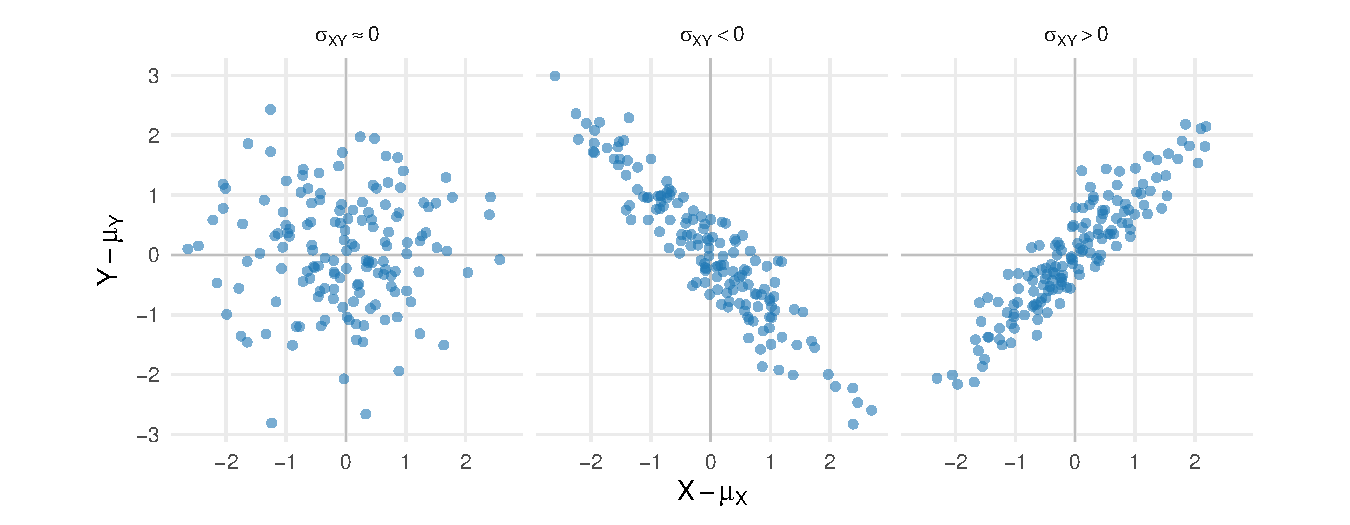
\includegraphics[keepaspectratio]{mod_2_covariancias_files/figure-pdf/fig-covariancia-padroes-1.pdf}}

}

\caption{\label{fig-covariancia-padroes}Padrões de dispersão associados
ao sinal da covariância.}

\end{figure}%

Na primeira configuração, a nuvem de pontos tende a se alongar em uma
direção crescente; na terceira, em uma direção decrescente. A
configuração central não apresenta orientação linear predominante. O
valor da covariância depende também das escalas das variáveis e, por
isso, seu módulo não fornece isoladamente uma medida comparável de
intensidade entre diferentes pares de variáveis.

Expandindo o produto dos desvios,

\[
\begin{aligned}
\operatorname{Cov}(X,Y)
&=
E
\left[
(X-\mu_X)(Y-\mu_Y)
\right]\\
&=
E(XY)
-
\mu_XE(Y)
-
\mu_YE(X)
+
\mu_X\mu_Y.
\end{aligned}
\]

Como \(E(X)=\mu_X\) e \(E(Y)=\mu_Y\),

\begin{equation}\phantomsection\label{eq-covariancia-forma-expandida}{
\operatorname{Cov}(X,Y)
=
E(XY)
-
E(X)E(Y).
}\end{equation}

A expressão Equação~\ref{eq-covariancia-forma-expandida} relaciona a
covariância ao momento conjunto \(E(XY)\) e aos primeiros momentos das
duas variáveis.

Quando as duas variáveis coincidem,

\[
\operatorname{Cov}(X,X)
=
E
\left[
(X-\mu_X)^2
\right]
=
\operatorname{Var}(X).
\]

A covariância também é simétrica:

\[
\operatorname{Cov}(X,Y)
=
\operatorname{Cov}(Y,X).
\]

Para constantes \(a\), \(b\), \(c\) e \(d\),

\begin{equation}\phantomsection\label{eq-transformacao-covariancia-escalar}{
\operatorname{Cov}(aX+b,cY+d)
=
ac\operatorname{Cov}(X,Y).
}\end{equation}

A identidade Equação~\ref{eq-transformacao-covariancia-escalar} mostra
que translações não alteram a covariância. Mudanças de escala
multiplicam a covariância pelo produto dos fatores aplicados às duas
variáveis. Quando somente um desses fatores é negativo, o sinal da
covariância é invertido.

Essa dependência das unidades impede a comparação direta entre
covariâncias associadas a pares de variáveis em escalas distintas. Se
uma variável medida em metros for convertida para centímetros, por
exemplo, sua covariância com outra variável será multiplicada por
\(100\).

Pela desigualdade de Cauchy--Schwarz,

\begin{equation}\phantomsection\label{eq-limite-covariancia}{
\left|
\operatorname{Cov}(X,Y)
\right|
\leq
\sqrt{
\operatorname{Var}(X)
\operatorname{Var}(Y)
}.
}\end{equation}

O limite Equação~\ref{eq-limite-covariancia} será utilizado
posteriormente para mostrar que a correlação pertence ao intervalo
\([-1,1]\).

\begin{tcolorbox}[enhanced jigsaw, colback=white, breakable, bottomrule=.15mm, left=2mm, arc=.35mm, rightrule=.15mm, colframe=quarto-callout-caution-color-frame, toprule=.15mm, leftrule=.75mm, opacityback=0]

\vspace{-3mm}\textbf{Covariância nula e independência}\vspace{3mm}

Covariância nula não implica independência em uma distribuição geral. A
covariância registra associação linear de segunda ordem, e relações não
lineares podem produzir covariância igual a zero.

\end{tcolorbox}

\begin{example}[Dependência não linear com covariância
nula]\protect\hypertarget{exm-dependencia-covariancia-nula}{}\label{exm-dependencia-covariancia-nula}

Considere

\[
X
\sim
\operatorname{Uniforme}(-2,2)
\]

e

\[
Y
=
X^2+\varepsilon,
\]

em que \(\varepsilon\) é independente de \(X\), possui média zero e
segundo momento finito.

A simetria da distribuição de \(X\) em torno de zero implica

\[
E(X)
=
0
\qquad
\text{e}
\qquad
E(X^3)
=
0.
\]

Como \(\varepsilon\) é independente de \(X\),

\[
E(X\varepsilon)
=
E(X)E(\varepsilon)
=
0.
\]

Para calcular a covariância entre \(X\) e \(Y\), utiliza-se

\[
\operatorname{Cov}(X,Y)
=
E(XY)-E(X)E(Y).
\]

Como \(Y=X^2+\varepsilon\),

\[
\begin{aligned}
E(XY)
&=
E\left[
X\left(X^2+\varepsilon\right)
\right]\\
&=
E(X^3)
+
E(X\varepsilon)\\
&=
0.
\end{aligned}
\]

Além disso,

\[
E(X)E(Y)
=
0,
\]

pois \(E(X)=0\). Portanto,

\[
\operatorname{Cov}(X,Y)
=
E(XY)-E(X)E(Y)
=
0.
\]

Apesar da covariância nula, \(X\) e \(Y\) não são independentes. Para
verificar isso, considere a esperança condicional de \(Y\) dado \(X=x\).
Como \[
\begin{aligned}
E(Y\mid X=x)
&=
E\left(X^2+\varepsilon\mid X=x\right)\\
&=
x^2
+
E(\varepsilon\mid X=x).
\end{aligned}
\]

Como \(\varepsilon\) é independente de \(X\),

\[
E(\varepsilon\mid X=x)
=
E(\varepsilon)
=
0.
\]

Portanto,

\[
E(Y\mid X=x)
=
x^2.
\]

Assim, a média condicional de \(Y\) depende do valor de \(X\). Se \(X\)
e \(Y\) fossem independentes, a distribuição condicional de \(Y\) dado
\(X=x\) seria a mesma distribuição marginal de \(Y\) e,
consequentemente,

\[
E(Y\mid X=x)
=
E(Y),
\]

não dependendo de \(x\). Logo, \(X\) e \(Y\) são dependentes, apesar de
apresentarem covariância nula.

A Figura~\ref{fig-dependencia-covariancia-nula} ilustra essa relação.

\begin{figure}

\centering{

\pandocbounded{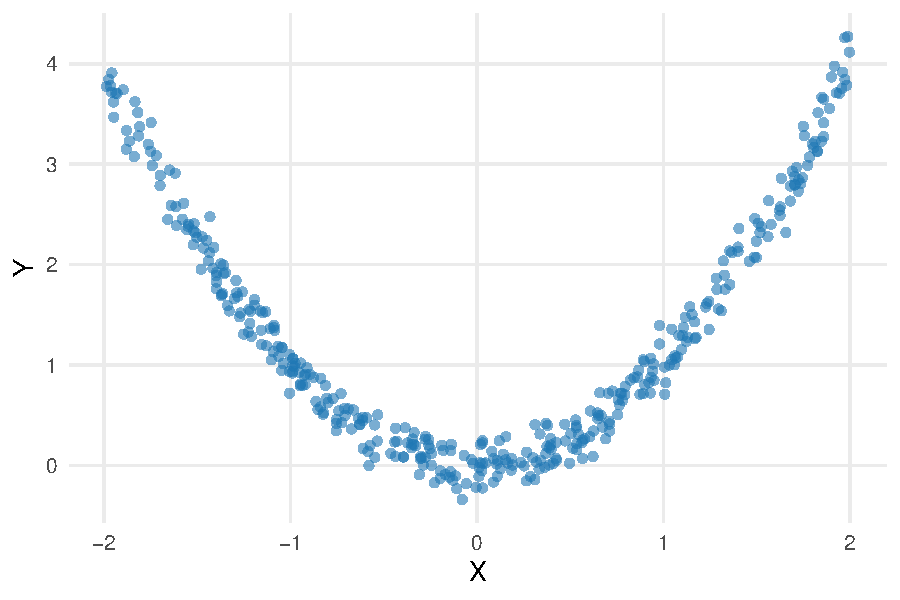
\includegraphics[keepaspectratio]{mod_2_covariancias_files/figure-pdf/fig-dependencia-covariancia-nula-1.pdf}}

}

\caption{\label{fig-dependencia-covariancia-nula}Dependência não linear
com covariância aproximadamente nula na amostra simulada.}

\end{figure}%

A configuração parabólica evidencia uma dependência que não produz
orientação linear global. O exemplo delimita a informação fornecida pela
covariância e mostra por que o valor zero não deve ser interpretado, sem
hipóteses adicionais, como independência.

\end{example}

As variâncias das componentes e as covariâncias entre todos os pares de
componentes podem ser reunidas em uma única matriz.

\section{Matriz de covariâncias
populacional}\label{matriz-de-covariuxe2ncias-populacional}

\subsection{Definição e interpretação dos
elementos}\label{definiuxe7uxe3o-e-interpretauxe7uxe3o-dos-elementos}

\begin{definition}[Matriz de covariâncias
populacional]\protect\hypertarget{def-matriz-covariancias-populacional}{}\label{def-matriz-covariancias-populacional}

Seja \(\boldsymbol{\mathsf X}\in\mathbb{R}^p\) um vetor aleatório com
vetor de médias \(\boldsymbol{\mu}\) e segundos momentos finitos. A
\textbf{matriz de covariâncias populacional} de
\(\boldsymbol{\mathsf X}\) é

\begin{equation}\phantomsection\label{eq-definicao-matriz-covariancias}{
\boldsymbol{\Sigma}
=
\operatorname{Cov}
\left(
\boldsymbol{\mathsf X}
\right)
=
E
\left[
\left(
\boldsymbol{\mathsf X}
-
\boldsymbol{\mu}
\right)
\left(
\boldsymbol{\mathsf X}
-
\boldsymbol{\mu}
\right)^{\top}
\right]
\in
\mathbb{R}^{p\times p}.
}\end{equation}

\end{definition}

O elemento situado na linha \(j\) e na coluna \(k\) de
\(\boldsymbol{\Sigma}\) é

\[
\sigma_{jk}
=
\operatorname{Cov}(X_j,X_k),
\qquad
j,k=1,\ldots,p.
\]

Assim,

\begin{equation}\phantomsection\label{eq-matriz-covariancias-elementos}{
\boldsymbol{\Sigma}
=
\begin{bmatrix}
\operatorname{Var}(X_1)
&
\operatorname{Cov}(X_1,X_2)
&
\cdots
&
\operatorname{Cov}(X_1,X_p)
\\
\operatorname{Cov}(X_2,X_1)
&
\operatorname{Var}(X_2)
&
\cdots
&
\operatorname{Cov}(X_2,X_p)
\\
\vdots
&
\vdots
&
\ddots
&
\vdots
\\
\operatorname{Cov}(X_p,X_1)
&
\operatorname{Cov}(X_p,X_2)
&
\cdots
&
\operatorname{Var}(X_p)
\end{bmatrix}.
}\end{equation}

Os elementos da diagonal principal são as variâncias,

\[
\sigma_{jj}
=
\operatorname{Var}(X_j),
\]

e os elementos fora da diagonal são as covariâncias entre componentes
distintos.

Como

\[
\operatorname{Cov}(X_j,X_k)
=
\operatorname{Cov}(X_k,X_j),
\]

tem-se

\[
\sigma_{jk}
=
\sigma_{kj},
\]

e \(\boldsymbol{\Sigma}\) é simétrica. Para \(p\) componentes, existem
\(p\) variâncias e

\[
\frac{p(p-1)}{2}
\]

covariâncias distintas, totalizando

\[
\frac{p(p+1)}{2}
\]

elementos distintos.

As unidades dos elementos dependem das variáveis envolvidas. Se \(X_j\)
é medida em uma unidade \(u_j\), então

\[
\sigma_{jj}
\]

é expressa em \(u_j^2\). Para \(j\neq k\),

\[
\sigma_{jk}
\]

é expressa em \(u_ju_k\). Essa dependência das unidades motiva a
construção posterior da matriz de correlações.

\subsection{Variâncias e covariâncias de combinações
lineares}\label{variuxe2ncias-e-covariuxe2ncias-de-combinauxe7uxf5es-lineares}

Uma combinação linear das componentes de \(\boldsymbol{\mathsf X}\)
possui a forma

\[
Y
=
\mathbf a^\top
\boldsymbol{\mathsf X},
\qquad
\mathbf a
\in
\mathbb{R}^p.
\]

O vetor \(\mathbf a\) contém os coeficientes da combinação e define uma
direção no espaço das variáveis. A combinação linear, já utilizada no
Módulo 1, adquire aqui uma interpretação probabilística: sua média e sua
variância são determinadas por \(\boldsymbol{\mu}\) e
\(\boldsymbol{\Sigma}\).

\begin{proposition}[Momentos de combinações
lineares]\protect\hypertarget{prp-momentos-combinacoes-lineares}{}\label{prp-momentos-combinacoes-lineares}

Seja \(\boldsymbol{\mathsf X}\in\mathbb{R}^p\) um vetor aleatório com
média \(\boldsymbol{\mu}\) e matriz de covariâncias
\(\boldsymbol{\Sigma}\). Para quaisquer vetores fixos
\(\mathbf a,\mathbf b\in\mathbb{R}^p\),

\begin{equation}\phantomsection\label{eq-media-combinacao-linear}{
E
\left(
\mathbf a^\top\boldsymbol{\mathsf X}
\right)
=
\mathbf a^\top\boldsymbol{\mu},
}\end{equation}

\begin{equation}\phantomsection\label{eq-variancia-combinacao-linear}{
\operatorname{Var}
\left(
\mathbf a^\top\boldsymbol{\mathsf X}
\right)
=
\mathbf a^\top
\boldsymbol{\Sigma}
\mathbf a,
}\end{equation}

e

\begin{equation}\phantomsection\label{eq-covariancia-combinacoes-lineares}{
\operatorname{Cov}
\left(
\mathbf a^\top\boldsymbol{\mathsf X},
\mathbf b^\top\boldsymbol{\mathsf X}
\right)
=
\mathbf a^\top
\boldsymbol{\Sigma}
\mathbf b.
}\end{equation}

\end{proposition}

\begin{proof}
Pela linearidade da esperança,

\[
E
\left(
\mathbf a^\top\boldsymbol{\mathsf X}
\right)
=
\mathbf a^\top
E(\boldsymbol{\mathsf X})
=
\mathbf a^\top\boldsymbol{\mu}.
\]

Além disso,

\[
\mathbf a^\top\boldsymbol{\mathsf X}
-
\mathbf a^\top\boldsymbol{\mu}
=
\mathbf a^\top
\left(
\boldsymbol{\mathsf X}
-
\boldsymbol{\mu}
\right).
\]

Consequentemente,

\[
\begin{aligned}
\operatorname{Var}
\left(
\mathbf a^\top\boldsymbol{\mathsf X}
\right)
&=
E
\left[
\mathbf a^\top
\left(
\boldsymbol{\mathsf X}
-
\boldsymbol{\mu}
\right)
\left(
\boldsymbol{\mathsf X}
-
\boldsymbol{\mu}
\right)^\top
\mathbf a
\right]\\
&=
\mathbf a^\top
\boldsymbol{\Sigma}
\mathbf a.
\end{aligned}
\]

De modo análogo,

\[
\begin{aligned}
&
\operatorname{Cov}
\left(
\mathbf a^\top\boldsymbol{\mathsf X},
\mathbf b^\top\boldsymbol{\mathsf X}
\right)
\\
&=
E
\left[
\mathbf a^\top
\left(
\boldsymbol{\mathsf X}
-
\boldsymbol{\mu}
\right)
\left(
\boldsymbol{\mathsf X}
-
\boldsymbol{\mu}
\right)^\top
\mathbf b
\right]\\
&=
\mathbf a^\top
\boldsymbol{\Sigma}
\mathbf b.
\end{aligned}
\]
\end{proof}

A expressão Equação~\ref{eq-variancia-combinacao-linear} mostra que a
matriz de covariâncias determina a variabilidade de todas as combinações
lineares das componentes. A quantidade

\[
\mathbf a^\top
\boldsymbol{\Sigma}
\mathbf a
\]

é uma forma quadrática no sentido de
Definição~\ref{def-forma-quadratica}. Quando \(\|\mathbf a\|=1\), ela
representa a variância da projeção de \(\boldsymbol{\mathsf X}\) sobre a
direção unitária \(\mathbf a\).

Essa relação constitui a ligação entre a matriz de covariâncias e a
geometria desenvolvida no Módulo 1: diferentes direções podem apresentar
diferentes níveis de dispersão.

\begin{example}[Matriz de covariâncias com três
variáveis]\protect\hypertarget{exm-matriz-covariancias-tres-variaveis}{}\label{exm-matriz-covariancias-tres-variaveis}

Considere

\[
\boldsymbol{\Sigma}
=
\begin{bmatrix}
4 & 1,5 & -0,8\\
1,5 & 9 & 0\\
-0,8 & 0 & 1
\end{bmatrix}.
\]

As variâncias das três componentes são

\[
\operatorname{Var}(X_1)
=
4,
\qquad
\operatorname{Var}(X_2)
=
9,
\qquad
\operatorname{Var}(X_3)
=
1,
\]

e as covariâncias distintas são

\[
\operatorname{Cov}(X_1,X_2)
=
1,5,
\]

\[
\operatorname{Cov}(X_1,X_3)
=
-0,8,
\]

e

\[
\operatorname{Cov}(X_2,X_3)
=
0.
\]

Considere a combinação linear

\[
Y
=
X_1
+
0,5X_2
-
X_3,
\]

com vetor de coeficientes

\[
\mathbf a
=
\begin{bmatrix}
1\\
0,5\\
-1
\end{bmatrix}.
\]

Pela expressão Equação~\ref{eq-variancia-combinacao-linear},

\[
\begin{aligned}
\operatorname{Var}(Y)
&=
\mathbf a^\top
\boldsymbol{\Sigma}
\mathbf a\\
&=
\begin{bmatrix}
1 & 0,5 & -1
\end{bmatrix}
\begin{bmatrix}
4 & 1,5 & -0,8\\
1,5 & 9 & 0\\
-0,8 & 0 & 1
\end{bmatrix}
\begin{bmatrix}
1\\
0,5\\
-1
\end{bmatrix}\\
&=
10,35.
\end{aligned}
\]

A variância da combinação depende das variâncias individuais, das
covariâncias e dos coeficientes utilizados. A covariância negativa entre
\(X_1\) e \(X_3\), por exemplo, contribui positivamente para
\(\operatorname{Var}(Y)\) porque os coeficientes dessas duas componentes
possuem sinais opostos.

\end{example}

\subsection{Propriedades estruturais e
singularidade}\label{propriedades-estruturais-e-singularidade}

A matriz de covariâncias pertence à classe das matrizes simétricas
positivas semidefinidas. A classificação de positividade de matrizes foi
estabelecida na Definição~\ref{def-classificacao-positividade}; aqui ela
adquire uma interpretação probabilística direta, pois a forma quadrática
associada a \(\boldsymbol{\Sigma}\) representa uma variância (Eaton,
2007).

\begin{proposition}[Caracterização estrutural das matrizes de
covariâncias]\protect\hypertarget{prp-estrutura-matriz-covariancias}{}\label{prp-estrutura-matriz-covariancias}

Uma matriz \(\mathbf C\in\mathbb{R}^{p\times p}\) é matriz de
covariâncias de algum vetor aleatório com segundos momentos finitos se,
e somente se,

\[
\mathbf C
=
\mathbf C^\top
\]

e

\[
\mathbf C
\succeq
\mathbf 0.
\]

Consequentemente, toda matriz de covariâncias possui elementos diagonais
não negativos, autovalores não negativos e submatrizes principais
positivas semidefinidas.

\end{proposition}

\begin{proof}
Se

\[
\mathbf C
=
\operatorname{Cov}
\left(
\boldsymbol{\mathsf X}
\right),
\]

a simetria decorre de

\[
\operatorname{Cov}(X_j,X_k)
=
\operatorname{Cov}(X_k,X_j).
\]

Além disso, para qualquer \(\mathbf a\in\mathbb{R}^p\),

\[
\mathbf a^\top
\mathbf C
\mathbf a
=
\operatorname{Var}
\left(
\mathbf a^\top
\boldsymbol{\mathsf X}
\right)
\geq
0.
\]

Logo, \(\mathbf C\) é positiva semidefinida.

Reciprocamente, suponha que \(\mathbf C\) seja real, simétrica e
positiva semidefinida. Pelo Teorema~\ref{thm-teorema-espectral} e pela
raiz quadrada principal definida na
Definição~\ref{def-raiz-quadrada-principal}, existe uma matriz simétrica
positiva semidefinida \(\mathbf C^{1/2}\) tal que

\[
\mathbf C
=
\mathbf C^{1/2}\mathbf C^{1/2}.
\]

Considere um vetor aleatório

\[
\boldsymbol{\mathsf U}
=
(U_1,\ldots,U_p)^\top,
\]

cujas componentes são independentes e satisfazem

\[
P(U_j=1)
=
P(U_j=-1)
=
\frac{1}{2},
\qquad
j=1,\ldots,p.
\]

Então,

\[
E
\left(
\boldsymbol{\mathsf U}
\right)
=
\mathbf 0
\]

e

\[
\operatorname{Cov}
\left(
\boldsymbol{\mathsf U}
\right)
=
\mathbf I_p.
\]

Defina

\[
\boldsymbol{\mathsf X}
=
\mathbf C^{1/2}
\boldsymbol{\mathsf U}.
\]

Como

\[
E
\left(
\boldsymbol{\mathsf U}
\right)
=
\mathbf 0,
\]

tem-se

\[
E
\left(
\boldsymbol{\mathsf X}
\right)
=
\mathbf C^{1/2}
E
\left(
\boldsymbol{\mathsf U}
\right)
=
\mathbf 0.
\]

Além disso,

\[
E
\left(
\boldsymbol{\mathsf U}
\boldsymbol{\mathsf U}^{\top}
\right)
=
\mathbf I_p.
\]

Logo,

\[
\begin{aligned}
\operatorname{Cov}
\left(
\boldsymbol{\mathsf X}
\right)
&=
E
\left(
\boldsymbol{\mathsf X}
\boldsymbol{\mathsf X}^{\top}
\right)\\
&=
E
\left(
\mathbf C^{1/2}
\boldsymbol{\mathsf U}
\boldsymbol{\mathsf U}^{\top}
\mathbf C^{1/2}
\right)\\
&=
\mathbf C^{1/2}
E
\left(
\boldsymbol{\mathsf U}
\boldsymbol{\mathsf U}^{\top}
\right)
\mathbf C^{1/2}\\
&=
\mathbf C^{1/2}
\mathbf I_p
\mathbf C^{1/2}\\
&=
\mathbf C.
\end{aligned}
\]

Portanto, toda matriz real simétrica positiva semidefinida pode ocorrer
como matriz de covariâncias.
\end{proof}

Essa construção estabelece apenas a existência de um vetor aleatório com
matriz de covariâncias \(\mathbf C\) e não exige uma família de
distribuições específica.

A semidefinição positiva impõe restrições aos elementos da matriz. Para
duas componentes \(X_j\) e \(X_k\), a submatriz principal

\[
\begin{bmatrix}
\sigma_{jj} & \sigma_{jk}\\
\sigma_{jk} & \sigma_{kk}
\end{bmatrix}
\]

também deve ser positiva semidefinida. Logo,

\[
\sigma_{jj}\sigma_{kk}
-
\sigma_{jk}^2
\geq
0,
\]

o que equivale a

\[
|\sigma_{jk}|
\leq
\sqrt{
\sigma_{jj}\sigma_{kk}
}.
\]

Esse resultado recupera, no nível matricial, o limite apresentado na
Equação~\ref{eq-limite-covariancia}.

A simetria, isoladamente, não é suficiente para caracterizar uma matriz
de covariâncias.

\begin{example}[Matriz simétrica que não pode ser uma matriz de
covariâncias]\protect\hypertarget{exm-matriz-simetrica-invalida-covariancia}{}\label{exm-matriz-simetrica-invalida-covariancia}

Considere

\[
\mathbf A
=
\begin{bmatrix}
1 & 2\\
2 & 1
\end{bmatrix}.
\]

A matriz é simétrica. Entretanto, para

\[
\mathbf a
=
\begin{bmatrix}
1\\
-1
\end{bmatrix},
\]

tem-se

\[
\begin{aligned}
\mathbf a^\top
\mathbf A
\mathbf a
&=
\begin{bmatrix}
1 & -1
\end{bmatrix}
\begin{bmatrix}
1 & 2\\
2 & 1
\end{bmatrix}
\begin{bmatrix}
1\\
-1
\end{bmatrix}\\
&=
-2.
\end{aligned}
\]

Se \(\mathbf A\) fosse uma matriz de covariâncias, esse valor
representaria a variância de uma combinação linear, o que é impossível.
A matriz é, portanto, simétrica, mas não positiva semidefinida.

\end{example}

Quando

\[
\mathbf a^\top
\boldsymbol{\Sigma}
\mathbf a
>
0
\]

para todo \(\mathbf a\neq\mathbf 0\), a matriz \(\boldsymbol{\Sigma}\) é
positiva definida. Pela Equação~\ref{eq-variancia-combinacao-linear},
isso significa que toda combinação linear não trivial das componentes
possui variância positiva.

A situação muda quando \(\boldsymbol{\Sigma}\) é singular. Nesse caso,
aparecerá a expressão \textbf{quase certamente}. Seja \(U\) uma variável
aleatória definida em um espaço de probabilidade
\((\Omega,\mathcal{F},P)\) e seja \(c\in\mathbb{R}\). Escrever

\[
U=c
\qquad
\text{quase certamente}
\]

significa que

\[
P\left(
\{\omega\in\Omega:U(\omega)=c\}
\right)
=
P(U=c)
=
1.
\]

Equivalentemente, a igualdade pode falhar apenas em um conjunto de
resultados de probabilidade zero.

\begin{proposition}[Caracterização da singularidade da matriz de
covariâncias]\protect\hypertarget{prp-singularidade-matriz-covariancias}{}\label{prp-singularidade-matriz-covariancias}

Seja \(\boldsymbol{\mathsf X}\in\mathbb{R}^p\) um vetor aleatório com
média \(\boldsymbol{\mu}\) e matriz de covariâncias
\(\boldsymbol{\Sigma}\). As seguintes afirmações são equivalentes:

\begin{enumerate}
\def\labelenumi{\arabic{enumi}.}
\item
  \(\boldsymbol{\Sigma}\) é singular;
\item
  existe \(\mathbf a\neq\mathbf 0\) tal que

  \[
  \mathbf a^\top
  \boldsymbol{\Sigma}
  \mathbf a
  =
  0;
  \]
\item
  existe \(\mathbf a\neq\mathbf 0\) tal que

  \[
  \operatorname{Var}
  \left(
  \mathbf a^\top
  \boldsymbol{\mathsf X}
  \right)
  =
  0;
  \]
\item
  existe \(\mathbf a\neq\mathbf 0\) tal que

  \[
  \mathbf a^\top
  \left(
  \boldsymbol{\mathsf X}
  -
  \boldsymbol{\mu}
  \right)
  =
  0
  \qquad
  \text{quase certamente}.
  \]
\end{enumerate}

\end{proposition}

\begin{proof}
Como \(\boldsymbol{\Sigma}\) é simétrica e positiva semidefinida, o
Teorema~\ref{thm-teorema-espectral} garante uma decomposição com
autovalores não negativos. A matriz é singular se, e somente se, pelo
menos um desses autovalores é zero. Nesse caso, existe
\(\mathbf a\neq\mathbf 0\) no núcleo de \(\boldsymbol{\Sigma}\) e,
portanto,

\[
\mathbf a^\top
\boldsymbol{\Sigma}
\mathbf a
=
0.
\]

Reciprocamente, para uma matriz positiva semidefinida,

\[
\mathbf a^\top
\boldsymbol{\Sigma}
\mathbf a
=
0
\]

implica que \(\mathbf a\) pertence ao núcleo de \(\boldsymbol{\Sigma}\).

Pela Equação~\ref{eq-variancia-combinacao-linear},

\[
\mathbf a^\top
\boldsymbol{\Sigma}
\mathbf a
=
\operatorname{Var}
\left(
\mathbf a^\top
\boldsymbol{\mathsf X}
\right),
\]

o que estabelece a equivalência entre as duas condições seguintes.

Uma variável aleatória possui variância zero se, e somente se, é
constante quase certamente. Como

\[
E
\left[
\mathbf a^\top
\left(
\boldsymbol{\mathsf X}
-
\boldsymbol{\mu}
\right)
\right]
=
0,
\]

essa constante deve ser zero. Portanto,

\[
\operatorname{Var}
\left(
\mathbf a^\top
\boldsymbol{\mathsf X}
\right)
=
0
\]

se, e somente se,

\[
\mathbf a^\top
\left(
\boldsymbol{\mathsf X}
-
\boldsymbol{\mu}
\right)
=
0
\qquad
\text{quase certamente}.
\]
\end{proof}

A última condição da
Proposição~\ref{prp-singularidade-matriz-covariancias} também pode ser
escrita como

\[
\mathbf a^\top
\boldsymbol{\mathsf X}
=
\mathbf a^\top
\boldsymbol{\mu}
\qquad
\text{quase certamente}.
\]

Portanto, a singularidade de \(\boldsymbol{\Sigma}\) corresponde à
existência de uma relação afim exata e não trivial entre as componentes
do vetor aleatório.

Em termos geométricos, os vetores pertencentes a

\[
\mathcal{N}
\left(
\boldsymbol{\Sigma}
\right)
\]

determinam direções de variância nula. Como \(\boldsymbol{\Sigma}\) é
simétrica, a relação entre núcleo e espaço coluna desenvolvida no Módulo
1 permite escrever

\[
\mathcal{N}
\left(
\boldsymbol{\Sigma}
\right)^\perp
=
\mathcal{C}
\left(
\boldsymbol{\Sigma}
\right).
\]

Consequentemente,

\[
\boldsymbol{\mathsf X}
-
\boldsymbol{\mu}
\in
\mathcal{C}
\left(
\boldsymbol{\Sigma}
\right)
\qquad
\text{quase certamente}.
\]

Se

\[
\operatorname{posto}
\left(
\boldsymbol{\Sigma}
\right)
=
r
<
p,
\]

a variabilidade do vetor centralizado está restrita a um subespaço de
dimensão \(r\). O vetor original está, portanto, restrito quase
certamente ao subespaço afim

\[
\boldsymbol{\mu}
+
\mathcal{C}
\left(
\boldsymbol{\Sigma}
\right).
\]

A matriz de covariâncias também pode ser utilizada para descrever
conjuntamente dois vetores aleatórios distintos. Essa extensão produz
matrizes retangulares de covariâncias cruzadas e permite representar as
relações lineares entre dois blocos de variáveis.

\section{Covariâncias entre vetores e
transformações}\label{covariuxe2ncias-entre-vetores-e-transformauxe7uxf5es}

\subsection{Covariâncias cruzadas e vetores
particionados}\label{covariuxe2ncias-cruzadas-e-vetores-particionados}

A covariância pode relacionar componentes pertencentes a dois vetores
aleatórios distintos. Considere

\[
\boldsymbol{\mathsf X}
\in
\mathbb{R}^p
\qquad
\text{e}
\qquad
\boldsymbol{\mathsf Y}
\in
\mathbb{R}^q,
\]

com vetores de médias

\[
\boldsymbol{\mu}_X
=
E
\left(
\boldsymbol{\mathsf X}
\right)
\in
\mathbb{R}^p
\]

e

\[
\boldsymbol{\mu}_Y
=
E
\left(
\boldsymbol{\mathsf Y}
\right)
\in
\mathbb{R}^q.
\]

Admite-se que todas as componentes possuam segundos momentos finitos.

\begin{definition}[Matriz de covariâncias
cruzadas]\protect\hypertarget{def-covariancia-cruzada}{}\label{def-covariancia-cruzada}

A \textbf{matriz de covariâncias cruzadas} entre
\(\boldsymbol{\mathsf X}\) e \(\boldsymbol{\mathsf Y}\) é

\begin{equation}\phantomsection\label{eq-definicao-covariancia-cruzada}{
\boldsymbol{\Sigma}_{XY}
=
\operatorname{Cov}
\left(
\boldsymbol{\mathsf X},
\boldsymbol{\mathsf Y}
\right)
=
E
\left[
\left(
\boldsymbol{\mathsf X}
-
\boldsymbol{\mu}_X
\right)
\left(
\boldsymbol{\mathsf Y}
-
\boldsymbol{\mu}_Y
\right)^\top
\right]
\in
\mathbb{R}^{p\times q},
}\end{equation}

em que \(\boldsymbol{\mathsf X}\in\mathbb R^p\) e
\(\boldsymbol{\mathsf Y}\in\mathbb R^q\) possuem segundos momentos
finitos e médias \(\boldsymbol{\mu}_X\) e \(\boldsymbol{\mu}_Y\),
respectivamente.

\end{definition}

O elemento situado na linha \(j\) e na coluna \(k\) é

\[
\left(
\boldsymbol{\Sigma}_{XY}
\right)_{jk}
=
\operatorname{Cov}
\left(
X_j,Y_k
\right),
\]

para \(j=1,\ldots,p\) e \(k=1,\ldots,q\). Portanto,

\[
\boldsymbol{\Sigma}_{XY}
=
\begin{bmatrix}
\operatorname{Cov}(X_1,Y_1)
&
\cdots
&
\operatorname{Cov}(X_1,Y_q)
\\
\vdots
&
\ddots
&
\vdots
\\
\operatorname{Cov}(X_p,Y_1)
&
\cdots
&
\operatorname{Cov}(X_p,Y_q)
\end{bmatrix}.
\]

A orientação da matriz depende da ordem dos vetores. Invertendo essa
ordem,

\begin{equation}\phantomsection\label{eq-transposta-covariancia-cruzada}{
\boldsymbol{\Sigma}_{YX}
=
\boldsymbol{\Sigma}_{XY}^{\top}.
}\end{equation}

Assim,

\[
\boldsymbol{\Sigma}_{XY}
\in
\mathbb{R}^{p\times q},
\qquad
\boldsymbol{\Sigma}_{YX}
\in
\mathbb{R}^{q\times p}.
\]

Mesmo quando \(p=q\), não se tem em geral

\[
\boldsymbol{\Sigma}_{XY}
=
\boldsymbol{\Sigma}_{YX},
\]

pois uma matriz de covariâncias cruzadas não precisa ser simétrica.

\begin{proposition}[Covariância entre combinações de dois
vetores]\protect\hypertarget{prp-covariancia-combinacoes-blocos}{}\label{prp-covariancia-combinacoes-blocos}

Sejam \(\boldsymbol{\mathsf X}\in\mathbb R^p\) e
\(\boldsymbol{\mathsf Y}\in\mathbb R^q\) vetores aleatórios com matriz
de covariâncias cruzadas \(\boldsymbol{\Sigma}_{XY}\). Para quaisquer
vetores fixos

\[
\mathbf a
\in
\mathbb{R}^p
\qquad
\text{e}
\qquad
\mathbf b
\in
\mathbb{R}^q,
\]

tem-se

\begin{equation}\phantomsection\label{eq-covariancia-combinacoes-blocos}{
\operatorname{Cov}
\left(
\mathbf a^\top\boldsymbol{\mathsf X},
\mathbf b^\top\boldsymbol{\mathsf Y}
\right)
=
\mathbf a^\top
\boldsymbol{\Sigma}_{XY}
\mathbf b.
}\end{equation}

\end{proposition}

\begin{proof}
As versões centralizadas das duas combinações são

\[
\mathbf a^\top
\left(
\boldsymbol{\mathsf X}
-
\boldsymbol{\mu}_X
\right)
\]

e

\[
\mathbf b^\top
\left(
\boldsymbol{\mathsf Y}
-
\boldsymbol{\mu}_Y
\right).
\]

Logo,

\[
\begin{aligned}
&
\operatorname{Cov}
\left(
\mathbf a^\top\boldsymbol{\mathsf X},
\mathbf b^\top\boldsymbol{\mathsf Y}
\right)
\\
&=
E
\left[
\mathbf a^\top
\left(
\boldsymbol{\mathsf X}
-
\boldsymbol{\mu}_X
\right)
\left(
\boldsymbol{\mathsf Y}
-
\boldsymbol{\mu}_Y
\right)^\top
\mathbf b
\right]
\\
&=
\mathbf a^\top
\boldsymbol{\Sigma}_{XY}
\mathbf b.
\end{aligned}
\]
\end{proof}

Em particular,

\[
\boldsymbol{\Sigma}_{XY}
=
\mathbf 0
\]

se, e somente se,

\[
\operatorname{Cov}
\left(
\mathbf a^\top\boldsymbol{\mathsf X},
\mathbf b^\top\boldsymbol{\mathsf Y}
\right)
=
0
\]

para todos os vetores \(\mathbf a\in\mathbb{R}^p\) e
\(\mathbf b\in\mathbb{R}^q\). Nesse caso, nenhuma combinação linear do
primeiro bloco possui covariância não nula com uma combinação linear do
segundo.

A condição

\[
\boldsymbol{\Sigma}_{XY}
=
\mathbf 0
\]

não implica, em uma distribuição geral, independência entre os vetores.
Essa relação será retomada no Capítulo 9 sob a distribuição normal
multivariada.

Os dois vetores podem ser reunidos em um único vetor particionado:

\[
\boldsymbol{\mathsf V}
=
\begin{bmatrix}
\boldsymbol{\mathsf X}\\
\boldsymbol{\mathsf Y}
\end{bmatrix}
\in
\mathbb{R}^{p+q}.
\]

Seu vetor de médias é

\[
\boldsymbol{\mu}_V
=
\begin{bmatrix}
\boldsymbol{\mu}_X\\
\boldsymbol{\mu}_Y
\end{bmatrix},
\]

e sua matriz de covariâncias pode ser representada por blocos, conforme
a estrutura de matrizes particionadas definida na
Definição~\ref{def-matriz-particionada}:

\begin{equation}\phantomsection\label{eq-covariancia-vetor-particionado}{
\boldsymbol{\Sigma}_V
=
\begin{bmatrix}
\boldsymbol{\Sigma}_{XX}
&
\boldsymbol{\Sigma}_{XY}
\\
\boldsymbol{\Sigma}_{YX}
&
\boldsymbol{\Sigma}_{YY}
\end{bmatrix},
}\end{equation}

em que

\[
\boldsymbol{\Sigma}_{XX}
=
\operatorname{Cov}
\left(
\boldsymbol{\mathsf X}
\right)
\]

e

\[
\boldsymbol{\Sigma}_{YY}
=
\operatorname{Cov}
\left(
\boldsymbol{\mathsf Y}
\right).
\]

Os blocos diagonais descrevem a dispersão interna de cada vetor,
enquanto os blocos fora da diagonal descrevem as covariâncias entre suas
componentes.

Como \(\boldsymbol{\Sigma}_V\) é uma matriz de covariâncias, ela é
simétrica e positiva semidefinida. Essa condição restringe conjuntamente
seus blocos. Em particular, \(\boldsymbol{\Sigma}_{XY}\) não pode ser
especificada arbitrariamente depois de fixadas
\(\boldsymbol{\Sigma}_{XX}\) e \(\boldsymbol{\Sigma}_{YY}\).

\subsubsection{Complemento de Schur e dispersão
residual}\label{complemento-de-schur-e-dispersuxe3o-residual}

O complemento de Schur já foi definido na
Definição~\ref{def-complemento-schur}. Aplicado à matriz de covariâncias
particionada, ele recebe uma interpretação estatística de segunda ordem.

Suponha que

\[
\boldsymbol{\Sigma}_{YY}
\succ
\mathbf 0.
\]

O complemento de Schur de \(\boldsymbol{\Sigma}_{YY}\) em
\(\boldsymbol{\Sigma}_V\) é

\begin{equation}\phantomsection\label{eq-complemento-schur-covariancia}{
\boldsymbol{\Sigma}_{XX\cdot Y}
=
\boldsymbol{\Sigma}_{XX}
-
\boldsymbol{\Sigma}_{XY}
\boldsymbol{\Sigma}_{YY}^{-1}
\boldsymbol{\Sigma}_{YX}.
}\end{equation}

Pelo resultado de positividade do complemento de Schur no
Teorema~\ref{thm-positividade-complemento-schur},

\[
\boldsymbol{\Sigma}_{XX\cdot Y}
\succeq
\mathbf 0.
\]

A expressão também pode ser interpretada diretamente como uma
covariância residual.

\begin{proposition}[Complemento de Schur e covariância
residual]\protect\hypertarget{prp-complemento-schur-covariancia-residual}{}\label{prp-complemento-schur-covariancia-residual}

Sejam

\[
\boldsymbol{\mathsf X}
\in
\mathbb R^p
\qquad
\text{e}
\qquad
\boldsymbol{\mathsf Y}
\in
\mathbb R^q
\]

vetores aleatórios com segundos momentos finitos, vetores de médias

\[
\boldsymbol{\mu}_X
=
E
\left(
\boldsymbol{\mathsf X}
\right)
\qquad
\text{e}
\qquad
\boldsymbol{\mu}_Y
=
E
\left(
\boldsymbol{\mathsf Y}
\right),
\]

e matriz de covariâncias conjunta

\[
\operatorname{Cov}
\left(
\begin{bmatrix}
\boldsymbol{\mathsf X}\\
\boldsymbol{\mathsf Y}
\end{bmatrix}
\right)
=
\begin{bmatrix}
\boldsymbol{\Sigma}_{XX}
&
\boldsymbol{\Sigma}_{XY}\\
\boldsymbol{\Sigma}_{YX}
&
\boldsymbol{\Sigma}_{YY}
\end{bmatrix}.
\]

Se

\[
\boldsymbol{\Sigma}_{YY}
\succ
\mathbf0,
\]

o complemento de Schur

\[
\boldsymbol{\Sigma}_{XX\cdot Y}
=
\boldsymbol{\Sigma}_{XX}
-
\boldsymbol{\Sigma}_{XY}
\boldsymbol{\Sigma}_{YY}^{-1}
\boldsymbol{\Sigma}_{YX}
\]

é a menor matriz de covariâncias residuais, segundo a ordem de Loewner,
entre as matrizes obtidas ao aproximar linearmente
\(\boldsymbol{\mathsf X}_c\) por \(\mathbf L\boldsymbol{\mathsf Y}_c\),
com

\[
\mathbf L
\in
\mathbb R^{p\times q}.
\]

Para

\[
\mathbf L^\star
=
\boldsymbol{\Sigma}_{XY}
\boldsymbol{\Sigma}_{YY}^{-1},
\]

tem-se

\[
\operatorname{Cov}
\left(
\boldsymbol{\mathsf R}_{\mathbf L^\star}
\right)
=
\boldsymbol{\Sigma}_{XX\cdot Y},
\]

e, para qualquer

\[
\mathbf L
\in
\mathbb R^{p\times q},
\]

tem-se

\[
\operatorname{Cov}
\left(
\boldsymbol{\mathsf R}_{\mathbf L}
\right)
-
\boldsymbol{\Sigma}_{XX\cdot Y}
\succeq
\mathbf0,
\]

em que

\[
\boldsymbol{\mathsf R}_{\mathbf L}
=
\boldsymbol{\mathsf X}_c
-
\mathbf L
\boldsymbol{\mathsf Y}_c,
\]

\[
\boldsymbol{\mathsf X}_c
=
\boldsymbol{\mathsf X}
-
\boldsymbol{\mu}_X
\qquad
\text{e}
\qquad
\boldsymbol{\mathsf Y}_c
=
\boldsymbol{\mathsf Y}
-
\boldsymbol{\mu}_Y.
\]

\end{proposition}

\begin{proof}
Para uma matriz arbitrária \(\mathbf L\),

\[
\begin{aligned}
\operatorname{Cov}
\left(
\boldsymbol{\mathsf R}_{\mathbf L}
\right)
&=
\boldsymbol{\Sigma}_{XX}
-
\mathbf L
\boldsymbol{\Sigma}_{YX}
-
\boldsymbol{\Sigma}_{XY}
\mathbf L^\top
+
\mathbf L
\boldsymbol{\Sigma}_{YY}
\mathbf L^\top.
\end{aligned}
\]

Substituindo

\[
\mathbf L^\star
=
\boldsymbol{\Sigma}_{XY}
\boldsymbol{\Sigma}_{YY}^{-1},
\]

a expressão pode ser reorganizada como

\[
\begin{aligned}
\operatorname{Cov}
\left(
\boldsymbol{\mathsf R}_{\mathbf L}
\right)
&=
\boldsymbol{\Sigma}_{XX\cdot Y}
\\
&\quad+
\left(
\mathbf L-\mathbf L^\star
\right)
\boldsymbol{\Sigma}_{YY}
\left(
\mathbf L-\mathbf L^\star
\right)^\top.
\end{aligned}
\]

Como \(\boldsymbol{\Sigma}_{YY}\) é positiva definida,

\[
\left(
\mathbf L-\mathbf L^\star
\right)
\boldsymbol{\Sigma}_{YY}
\left(
\mathbf L-\mathbf L^\star
\right)^\top
\succeq
\mathbf 0.
\]

A diferença entre a covariância residual correspondente a qualquer
\(\mathbf L\) e aquela obtida com \(\mathbf L^\star\) é, portanto,
positiva semidefinida.
\end{proof}

Essa interpretação depende apenas dos segundos momentos e não exige
normalidade. Sob normalidade conjunta, o mesmo complemento de Schur
aparecerá no Capítulo 9 como matriz de covariâncias da distribuição
condicional de um bloco dado o outro.

\begin{example}[Covariâncias entre dois
blocos]\protect\hypertarget{exm-covariancia-cruzada-blocos}{}\label{exm-covariancia-cruzada-blocos}

Considere

\[
\boldsymbol{\mathsf X}
=
\begin{bmatrix}
X_1\\
X_2
\end{bmatrix}
\]

e

\[
\boldsymbol{\mathsf Y}
=
\begin{bmatrix}
Y_1\\
Y_2\\
Y_3
\end{bmatrix},
\]

com

\[
\boldsymbol{\Sigma}_{XY}
=
\begin{bmatrix}
2 & -1 & 0,5\\
1 & 3 & -2
\end{bmatrix}.
\]

Para as combinações

\[
U
=
X_1-2X_2
\]

e

\[
V
=
Y_1+Y_2,
\]

os vetores de coeficientes são

\[
\mathbf a
=
\begin{bmatrix}
1\\
-2
\end{bmatrix}
\]

e

\[
\mathbf b
=
\begin{bmatrix}
1\\
1\\
0
\end{bmatrix}.
\]

Pela expressão Equação~\ref{eq-covariancia-combinacoes-blocos},

\[
\begin{aligned}
\operatorname{Cov}(U,V)
&=
\mathbf a^\top
\boldsymbol{\Sigma}_{XY}
\mathbf b\\
&=
\begin{bmatrix}
1 & -2
\end{bmatrix}
\begin{bmatrix}
2 & -1 & 0,5\\
1 & 3 & -2
\end{bmatrix}
\begin{bmatrix}
1\\
1\\
0
\end{bmatrix}\\
&=
-7.
\end{aligned}
\]

A covariância entre \(U\) e \(V\) resulta conjuntamente das covariâncias
entre todas as componentes que participam das duas combinações lineares.

\end{example}

\subsection{Transformações afins da média e da
covariância}\label{transformauxe7uxf5es-afins-da-muxe9dia-e-da-covariuxe2ncia}

As transformações afins foram definidas na
Definição~\ref{def-transformacao-afim}. No contexto probabilístico,
interessa determinar como elas modificam a média e a matriz de
covariâncias.

Considere

\[
\boldsymbol{\mathsf U}
=
\mathbf A
\boldsymbol{\mathsf X}
+
\mathbf c,
\]

em que

\[
\boldsymbol{\mathsf X}
\in
\mathbb{R}^p,
\qquad
\mathbf A
\in
\mathbb{R}^{r\times p},
\qquad
\mathbf c
\in
\mathbb{R}^r.
\]

\begin{proposition}[Média e covariância sob transformação
afim]\protect\hypertarget{prp-transformacao-afim-covariancia}{}\label{prp-transformacao-afim-covariancia}

Seja \(\boldsymbol{\mathsf X}\in\mathbb R^p\) um vetor aleatório com
média \(\boldsymbol{\mu}_X\) e matriz de covariâncias
\(\boldsymbol{\Sigma}_{XX}\). Para

\[
\boldsymbol{\mathsf U}
=
\mathbf A
\boldsymbol{\mathsf X}
+
\mathbf c,
\qquad
\mathbf A\in\mathbb R^{r\times p},
\qquad
\mathbf c\in\mathbb R^r,
\]

tem-se

\begin{equation}\phantomsection\label{eq-media-transformacao-afim}{
E
\left(
\boldsymbol{\mathsf U}
\right)
=
\mathbf A
\boldsymbol{\mu}_X
+
\mathbf c
}\end{equation}

e

\begin{equation}\phantomsection\label{eq-covariancia-transformacao-afim}{
\operatorname{Cov}
\left(
\boldsymbol{\mathsf U}
\right)
=
\mathbf A
\boldsymbol{\Sigma}_{XX}
\mathbf A^\top.
}\end{equation}

\end{proposition}

\begin{proof}
Pela linearidade da esperança,

\[
E
\left(
\mathbf A\boldsymbol{\mathsf X}+\mathbf c
\right)
=
\mathbf A\boldsymbol{\mu}_X+\mathbf c.
\]

O vetor transformado centralizado é

\[
\begin{aligned}
\boldsymbol{\mathsf U}
-
E
\left(
\boldsymbol{\mathsf U}
\right)
&=
\mathbf A
\boldsymbol{\mathsf X}
+
\mathbf c
-
\mathbf A
\boldsymbol{\mu}_X
-
\mathbf c\\
&=
\mathbf A
\left(
\boldsymbol{\mathsf X}
-
\boldsymbol{\mu}_X
\right).
\end{aligned}
\]

Portanto,

\[
\begin{aligned}
\operatorname{Cov}
\left(
\boldsymbol{\mathsf U}
\right)
&=
E
\left[
\mathbf A
\left(
\boldsymbol{\mathsf X}
-
\boldsymbol{\mu}_X
\right)
\left(
\boldsymbol{\mathsf X}
-
\boldsymbol{\mu}_X
\right)^\top
\mathbf A^\top
\right]\\
&=
\mathbf A
\boldsymbol{\Sigma}_{XX}
\mathbf A^\top.
\end{aligned}
\]
\end{proof}

A ausência do vetor \(\mathbf c\) na
Equação~\ref{eq-covariancia-transformacao-afim} confirma que translações
alteram a localização, mas não a matriz de covariâncias.

Quando

\[
r=1
\qquad
\text{e}
\qquad
\mathbf A
=
\mathbf a^\top,
\]

a expressão reduz-se a

\[
\operatorname{Var}
\left(
\mathbf a^\top
\boldsymbol{\mathsf X}
\right)
=
\mathbf a^\top
\boldsymbol{\Sigma}_{XX}
\mathbf a,
\]

recuperando Equação~\ref{eq-variancia-combinacao-linear}.

Se \(\mathbf A\) é diagonal,

\[
\mathbf A
=
\operatorname{diag}
\left(
a_1,\ldots,a_p
\right),
\]

então

\[
\operatorname{Cov}
\left(
a_jX_j,a_kX_k
\right)
=
a_ja_k\sigma_{jk}.
\]

Em particular,

\[
\operatorname{Var}
\left(
a_jX_j
\right)
=
a_j^2\sigma_{jj}.
\]

Se \(\mathbf Q\in\mathbb{R}^{p\times p}\) é ortogonal no sentido de
Definição~\ref{def-matriz-ortogonal},

\[
\operatorname{Cov}
\left(
\mathbf Q\boldsymbol{\mathsf X}
\right)
=
\mathbf Q
\boldsymbol{\Sigma}_{XX}
\mathbf Q^\top.
\]

Como \(\mathbf Q^\top=\mathbf Q^{-1}\), essa transformação produz uma
matriz semelhante a \(\boldsymbol{\Sigma}_{XX}\) e preserva seus
autovalores. A interpretação estatística dessa propriedade será retomada
na geometria da covariância.

\begin{example}[Transformação de duas
variáveis]\protect\hypertarget{exm-transformacao-matriz-covariancias}{}\label{exm-transformacao-matriz-covariancias}

Considere

\[
\boldsymbol{\Sigma}_{XX}
=
\begin{bmatrix}
4 & 2\\
2 & 9
\end{bmatrix}
\]

e

\[
\boldsymbol{\mathsf U}
=
\mathbf A
\boldsymbol{\mathsf X},
\]

com

\[
\mathbf A
=
\begin{bmatrix}
1 & 1\\
1 & -1
\end{bmatrix}.
\]

As componentes transformadas são

\[
U_1
=
X_1+X_2
\]

e

\[
U_2
=
X_1-X_2.
\]

Pela expressão Equação~\ref{eq-covariancia-transformacao-afim},

\[
\begin{aligned}
\operatorname{Cov}
\left(
\boldsymbol{\mathsf U}
\right)
&=
\mathbf A
\boldsymbol{\Sigma}_{XX}
\mathbf A^\top\\
&=
\begin{bmatrix}
1 & 1\\
1 & -1
\end{bmatrix}
\begin{bmatrix}
4 & 2\\
2 & 9
\end{bmatrix}
\begin{bmatrix}
1 & 1\\
1 & -1
\end{bmatrix}\\
&=
\begin{bmatrix}
17 & -5\\
-5 & 9
\end{bmatrix}.
\end{aligned}
\]

Logo,

\[
\operatorname{Var}(U_1)
=
17,
\qquad
\operatorname{Var}(U_2)
=
9
\]

e

\[
\operatorname{Cov}(U_1,U_2)
=
-5.
\]

A transformação modifica simultaneamente as variâncias das componentes e
a covariância entre elas.

\end{example}

As covariâncias cruzadas também se transformam de maneira compatível.

\begin{proposition}[Covariância cruzada sob transformações
afins]\protect\hypertarget{prp-transformacao-covariancia-cruzada}{}\label{prp-transformacao-covariancia-cruzada}

Sejam \(\boldsymbol{\mathsf X}\in\mathbb R^p\) e
\(\boldsymbol{\mathsf Y}\in\mathbb R^q\) vetores aleatórios com matriz
de covariâncias cruzadas \(\boldsymbol{\Sigma}_{XY}\). Considere

\[
\boldsymbol{\mathsf U}
=
\mathbf A_X
\boldsymbol{\mathsf X}
+
\mathbf c
\]

e

\[
\boldsymbol{\mathsf V}
=
\mathbf A_Y
\boldsymbol{\mathsf Y}
+
\mathbf d,
\]

com

\[
\mathbf A_X
\in
\mathbb{R}^{r\times p},
\qquad
\mathbf A_Y
\in
\mathbb{R}^{s\times q},
\qquad
\mathbf c\in\mathbb R^r,
\qquad
\mathbf d\in\mathbb R^s.
\]

Então,

\begin{equation}\phantomsection\label{eq-transformacao-covariancia-cruzada}{
\operatorname{Cov}
\left(
\boldsymbol{\mathsf U},
\boldsymbol{\mathsf V}
\right)
=
\mathbf A_X
\boldsymbol{\Sigma}_{XY}
\mathbf A_Y^\top.
}\end{equation}

\end{proposition}

\begin{proof}
Após a centralização,

\[
\boldsymbol{\mathsf U}
-
E
\left(
\boldsymbol{\mathsf U}
\right)
=
\mathbf A_X
\left(
\boldsymbol{\mathsf X}
-
\boldsymbol{\mu}_X
\right)
\]

e

\[
\boldsymbol{\mathsf V}
-
E
\left(
\boldsymbol{\mathsf V}
\right)
=
\mathbf A_Y
\left(
\boldsymbol{\mathsf Y}
-
\boldsymbol{\mu}_Y
\right).
\]

Logo,

\[
\begin{aligned}
\operatorname{Cov}
\left(
\boldsymbol{\mathsf U},
\boldsymbol{\mathsf V}
\right)
&=
E
\left[
\mathbf A_X
\left(
\boldsymbol{\mathsf X}
-
\boldsymbol{\mu}_X
\right)
\left(
\boldsymbol{\mathsf Y}
-
\boldsymbol{\mu}_Y
\right)^\top
\mathbf A_Y^\top
\right]\\
&=
\mathbf A_X
\boldsymbol{\Sigma}_{XY}
\mathbf A_Y^\top.
\end{aligned}
\]
\end{proof}

As expressões Equação~\ref{eq-covariancia-transformacao-afim} e
Equação~\ref{eq-transformacao-covariancia-cruzada} mostram que a matriz
de covariâncias responde de maneira sistemática às transformações
lineares. A padronização das componentes constitui um caso particular
dessa estrutura.

\section{Padronização e matriz de
correlações}\label{padronizauxe7uxe3o-e-matriz-de-correlauxe7uxf5es}

\subsection{Matriz de correlações
populacional}\label{matriz-de-correlauxe7uxf5es-populacional}

As covariâncias dependem das unidades de medida das variáveis. Para
retirar as escalas marginais, suponha que

\[
\sigma_{jj}
=
\operatorname{Var}(X_j)
>
0,
\qquad
j=1,\ldots,p.
\]

Defina a matriz diagonal das variâncias populacionais por

\begin{equation}\phantomsection\label{eq-matriz-variancias-populacionais}{
\mathbf D_{\Sigma}
=
\operatorname{diag}
\left(
\sigma_{11},
\ldots,
\sigma_{pp}
\right).
}\end{equation}

Como todas as variâncias são positivas,

\[
\mathbf D_{\Sigma}
\succ
\mathbf 0
\]

e existem as matrizes diagonais

\[
\mathbf D_{\Sigma}^{1/2}
=
\operatorname{diag}
\left(
\sqrt{\sigma_{11}},
\ldots,
\sqrt{\sigma_{pp}}
\right)
\]

e

\[
\mathbf D_{\Sigma}^{-1/2}
=
\operatorname{diag}
\left(
\frac{1}{\sqrt{\sigma_{11}}},
\ldots,
\frac{1}{\sqrt{\sigma_{pp}}}
\right).
\]

\begin{definition}[Vetor aleatório
padronizado]\protect\hypertarget{def-vetor-padronizado-populacional}{}\label{def-vetor-padronizado-populacional}

Se \(\boldsymbol{\mathsf X}\in\mathbb R^p\) possui média
\(\boldsymbol{\mu}\) e variâncias marginais positivas, o vetor aleatório
marginalmente padronizado correspondente é

\begin{equation}\phantomsection\label{eq-vetor-padronizado-populacional}{
\boldsymbol{\mathsf Z}
=
\mathbf D_{\Sigma}^{-1/2}
\left(
\boldsymbol{\mathsf X}
-
\boldsymbol{\mu}
\right),
}\end{equation}

em que \(\mathbf D_{\Sigma}\succ\mathbf 0\) é a matriz diagonal das
variâncias populacionais e

\[
\mathbf D_{\Sigma}^{-1/2}
=
\operatorname{diag}
\left(
\frac{1}{\sqrt{\sigma_{11}}},
\ldots,
\frac{1}{\sqrt{\sigma_{pp}}}
\right).
\]

\end{definition}

Sua componente \(j\) é

\[
Z_j
=
\frac{
X_j-\mu_j
}{
\sqrt{\sigma_{jj}}
}.
\]

Assim,

\[
E(Z_j)
=
0
\]

e

\[
\operatorname{Var}(Z_j)
=
1.
\]

Em forma vetorial,

\[
E
\left(
\boldsymbol{\mathsf Z}
\right)
=
\mathbf 0.
\]

Aplicando Equação~\ref{eq-covariancia-transformacao-afim},

\[
\operatorname{Cov}
\left(
\boldsymbol{\mathsf Z}
\right)
=
\mathbf D_{\Sigma}^{-1/2}
\boldsymbol{\Sigma}
\mathbf D_{\Sigma}^{-1/2}.
\]

\begin{definition}[Matriz de correlações
populacional]\protect\hypertarget{def-matriz-correlacoes-populacional}{}\label{def-matriz-correlacoes-populacional}

A \textbf{matriz de correlações populacional} de
\(\boldsymbol{\mathsf X}\in\mathbb R^p\) é

\begin{equation}\phantomsection\label{eq-matriz-correlacoes-populacional}{
\boldsymbol{\mathcal R}
=
\mathbf D_{\Sigma}^{-1/2}
\boldsymbol{\Sigma}
\mathbf D_{\Sigma}^{-1/2},
}\end{equation}

em que \(\boldsymbol{\Sigma}\) é a matriz de covariâncias de
\(\boldsymbol{\mathsf X}\) e

\[
\mathbf D_{\Sigma}
=
\operatorname{diag}
\left(
\sigma_{11},
\ldots,
\sigma_{pp}
\right),
\]

com

\[
\sigma_{jj}
>
0,
\qquad
j=1,\ldots,p.
\]

\end{definition}

O símbolo \(\boldsymbol{\mathcal R}\) é reservado à matriz populacional.
Posteriormente, \(\boldsymbol{\mathsf R}\) representará a matriz de
correlações amostral, enquanto \(\mathbf R\) representará seu valor
calculado a partir de uma amostra observada.

A matriz \(\boldsymbol{\mathcal R}\) possui a forma

\[
\boldsymbol{\mathcal R}
=
\begin{bmatrix}
1
&
\rho_{12}
&
\cdots
&
\rho_{1p}
\\
\rho_{21}
&
1
&
\cdots
&
\rho_{2p}
\\
\vdots
&
\vdots
&
\ddots
&
\vdots
\\
\rho_{p1}
&
\rho_{p2}
&
\cdots
&
1
\end{bmatrix},
\]

em que

\begin{equation}\phantomsection\label{eq-correlacao-populacional}{
\rho_{jk}
=
\operatorname{Corr}
\left(
X_j,X_k
\right)
=
\frac{
\sigma_{jk}
}{
\sqrt{
\sigma_{jj}\sigma_{kk}
}
}.
}\end{equation}

Equivalentemente,

\[
\rho_{jk}
=
\operatorname{Cov}
\left(
Z_j,Z_k
\right).
\]

A correlação é adimensional porque o numerador e o denominador de
Equação~\ref{eq-correlacao-populacional} possuem as mesmas unidades.

A relação entre covariâncias e correlações pode ser invertida:

\begin{equation}\phantomsection\label{eq-recuperacao-covariancia-correlacao}{
\boldsymbol{\Sigma}
=
\mathbf D_{\Sigma}^{1/2}
\boldsymbol{\mathcal R}
\mathbf D_{\Sigma}^{1/2}.
}\end{equation}

Portanto, \(\boldsymbol{\Sigma}\) pode ser decomposta em dois elementos:

\begin{itemize}
\tightlist
\item
  \(\mathbf D_{\Sigma}\) registra as variâncias e, consequentemente, as
  escalas marginais;
\item
  \(\boldsymbol{\mathcal R}\) registra a estrutura de associação linear
  após a remoção dessas escalas.
\end{itemize}

A matriz de correlações isoladamente não permite recuperar as variâncias
originais.

\begin{example}[Matriz de correlações obtida por uma transformação de
padronização]\protect\hypertarget{exm-padronizacao-transformacao-covariancia}{}\label{exm-padronizacao-transformacao-covariancia}

Considere um vetor aleatório

\[
\boldsymbol{\mathsf X}
=
\begin{bmatrix}
X_1\\
X_2
\end{bmatrix}
\]

com vetor de médias \(\boldsymbol{\mu}\) e matriz de covariâncias

\[
\boldsymbol{\Sigma}
=
\begin{bmatrix}
16 & 12\\
12 & 25
\end{bmatrix}.
\]

Os desvios-padrão populacionais são

\[
\sqrt{\sigma_{11}}
=
4
\qquad
\text{e}
\qquad
\sqrt{\sigma_{22}}
=
5.
\]

Portanto,

\[
\mathbf D_{\Sigma}
=
\begin{bmatrix}
16 & 0\\
0 & 25
\end{bmatrix}
\]

e

\[
\mathbf D_{\Sigma}^{-1/2}
=
\begin{bmatrix}
1/4 & 0\\
0 & 1/5
\end{bmatrix}.
\]

Considere a transformação de padronização

\[
\boldsymbol{\mathsf Z}
=
\mathbf D_{\Sigma}^{-1/2}
\left(
\boldsymbol{\mathsf X}
-
\boldsymbol{\mu}
\right).
\]

Ela pode ser escrita como a transformação afim

\[
\boldsymbol{\mathsf Z}
=
\mathbf A
\boldsymbol{\mathsf X}
+
\mathbf c,
\]

com

\[
\mathbf A
=
\mathbf D_{\Sigma}^{-1/2}
\]

e

\[
\mathbf c
=
-
\mathbf D_{\Sigma}^{-1/2}
\boldsymbol{\mu}.
\]

Utilizando Proposição~\ref{prp-transformacao-afim-covariancia},

\[
\operatorname{Cov}
\left(
\boldsymbol{\mathsf Z}
\right)
=
\mathbf A
\boldsymbol{\Sigma}
\mathbf A^\top.
\]

Como \(\mathbf A\) é diagonal e simétrica,

\[
\begin{aligned}
\operatorname{Cov}
\left(
\boldsymbol{\mathsf Z}
\right)
&=
\begin{bmatrix}
1/4 & 0\\
0 & 1/5
\end{bmatrix}
\begin{bmatrix}
16 & 12\\
12 & 25
\end{bmatrix}
\begin{bmatrix}
1/4 & 0\\
0 & 1/5
\end{bmatrix}\\
&=
\begin{bmatrix}
1 & 3/5\\
3/5 & 1
\end{bmatrix}\\
&=
\begin{bmatrix}
1 & 0,6\\
0,6 & 1
\end{bmatrix}.
\end{aligned}
\]

Essa é precisamente a matriz de correlações populacional,

\[
\boldsymbol{\mathcal R}
=
\begin{bmatrix}
1 & 0,6\\
0,6 & 1
\end{bmatrix}.
\]

De fato,

\[
\rho_{12}
=
\frac{
\sigma_{12}
}{
\sqrt{
\sigma_{11}\sigma_{22}
}
}
=
\frac{12}{
\sqrt{16\cdot25}
}
=
\frac{12}{20}
=
0,6.
\]

O exemplo mostra duas formas equivalentes de chegar ao mesmo resultado.
Pela transformação do vetor,

\[
\text{padronizar } \boldsymbol{\mathsf X}
\quad\Longrightarrow\quad
\operatorname{Cov}
\left(
\boldsymbol{\mathsf Z}
\right).
\]

Equivalentemente, pode-se transformar diretamente a matriz de
covariâncias:

\[
\boldsymbol{\Sigma}
\quad\Longrightarrow\quad
\mathbf D_{\Sigma}^{-1/2}
\boldsymbol{\Sigma}
\mathbf D_{\Sigma}^{-1/2}.
\]

Em ambas as perspectivas, as variâncias tornam-se unitárias e a
covariância entre as componentes padronizadas passa a coincidir com sua
correlação.

\end{example}

\subsection{Propriedades, escala e
independência}\label{propriedades-escala-e-independuxeancia}

\begin{proposition}[Caracterização das matrizes de
correlações]\protect\hypertarget{prp-propriedades-matriz-correlacoes}{}\label{prp-propriedades-matriz-correlacoes}

Uma matriz

\[
\mathbf C
\in
\mathbb{R}^{p\times p}
\]

é matriz de correlações de algum vetor aleatório com variâncias
marginais positivas se, e somente se,

\[
\mathbf C
=
\mathbf C^\top,
\]

\[
\mathbf C
\succeq
\mathbf 0
\]

e

\[
c_{jj}
=
1,
\qquad
j=1,\ldots,p.
\]

Consequentemente, toda matriz de correlações possui:

\begin{enumerate}
\def\labelenumi{\arabic{enumi}.}
\tightlist
\item
  elementos no intervalo \([-1,1]\);
\item
  autovalores reais e não negativos;
\item
  traço igual a \(p\).
\end{enumerate}

\end{proposition}

\begin{proof}
Se \(\mathbf C=\boldsymbol{\mathcal R}\) é uma matriz de correlações,
então

\[
\boldsymbol{\mathcal R}
=
\mathbf D_{\Sigma}^{-1/2}
\boldsymbol{\Sigma}
\mathbf D_{\Sigma}^{-1/2}.
\]

Como \(\boldsymbol{\Sigma}\) é simétrica,

\[
\boldsymbol{\mathcal R}^{\top}
=
\boldsymbol{\mathcal R}.
\]

Além disso, para qualquer \(\mathbf a\in\mathbb{R}^p\),

\[
\begin{aligned}
\mathbf a^\top
\boldsymbol{\mathcal R}
\mathbf a
&=
\left(
\mathbf D_{\Sigma}^{-1/2}
\mathbf a
\right)^\top
\boldsymbol{\Sigma}
\left(
\mathbf D_{\Sigma}^{-1/2}
\mathbf a
\right)
\\
&\geq
0,
\end{aligned}
\]

de modo que

\[
\boldsymbol{\mathcal R}
\succeq
\mathbf 0.
\]

A diagonal é unitária porque

\[
\rho_{jj}
=
\frac{
\sigma_{jj}
}{
\sqrt{
\sigma_{jj}\sigma_{jj}
}
}
=
1.
\]

Reciprocamente, suponha que \(\mathbf C\) seja simétrica, positiva
semidefinida e possua diagonal unitária. Pela raiz quadrada principal
definida na Definição~\ref{def-raiz-quadrada-principal}, existe
\(\mathbf C^{1/2}\) tal que

\[
\mathbf C
=
\mathbf C^{1/2}
\mathbf C^{1/2}.
\]

Considere um vetor aleatório

\[
\boldsymbol{\mathsf U}
=
(U_1,\ldots,U_p)^\top,
\]

cujas componentes são independentes e satisfazem

\[
P(U_j=1)
=
P(U_j=-1)
=
\frac12.
\]

Então,

\[
E
\left(
\boldsymbol{\mathsf U}
\right)
=
\mathbf 0
\]

e

\[
\operatorname{Cov}
\left(
\boldsymbol{\mathsf U}
\right)
=
\mathbf I_p.
\]

Defina

\[
\boldsymbol{\mathsf Z}
=
\mathbf C^{1/2}
\boldsymbol{\mathsf U}.
\]

Tem-se

\[
\operatorname{Cov}
\left(
\boldsymbol{\mathsf Z}
\right)
=
\mathbf C^{1/2}
\mathbf I_p
\mathbf C^{1/2}
=
\mathbf C.
\]

Como a diagonal de \(\mathbf C\) é unitária, todas as componentes de
\(\boldsymbol{\mathsf Z}\) possuem variância igual a um. Logo, sua
matriz de covariâncias coincide com sua matriz de correlações, e
\(\mathbf C\) é uma matriz de correlações válida.

Pela desigualdade de Cauchy--Schwarz,

\[
|c_{jk}|
\leq
\sqrt{
c_{jj}c_{kk}
}
=
1.
\]

Como \(\mathbf C\) é simétrica e positiva semidefinida, seus autovalores
são reais e não negativos. Finalmente,

\[
\operatorname{tr}
\left(
\mathbf C
\right)
=
\sum_{j=1}^{p}c_{jj}
=
p.
\]
\end{proof}

Se \(\boldsymbol{\Sigma}\) possui variâncias marginais positivas, então
\(\mathbf D_{\Sigma}^{-1/2}\) é invertível e a padronização preserva a
definição positiva. Assim,

\[
\boldsymbol{\mathcal R}
\succ
\mathbf 0
\quad
\Longleftrightarrow
\quad
\boldsymbol{\Sigma}
\succ
\mathbf 0.
\]

Os valores extremos da correlação correspondem a relações lineares
exatas entre as variáveis padronizadas. Para \(j\neq k\),

\[
\rho_{jk}
=
1
\quad
\Longleftrightarrow
\quad
Z_k=Z_j
\qquad
\text{quase certamente},
\]

enquanto

\[
\rho_{jk}
=
-1
\quad
\Longleftrightarrow
\quad
Z_k=-Z_j
\qquad
\text{quase certamente}.
\]

Portanto, uma correlação de módulo igual a \(1\) implica uma relação
linear exata entre as duas variáveis e, consequentemente, a
singularidade da matriz de covariâncias do par correspondente.

Além disso, não basta que cada correlação, considerada isoladamente,
pertença ao intervalo \([-1,1]\) para que uma matriz seja uma matriz de
correlações válida; a matriz completa também deve ser positiva
semidefinida.

\begin{example}[Matriz com diagonal unitária que não é uma matriz de
correlações]\protect\hypertarget{exm-matriz-invalida-correlacoes}{}\label{exm-matriz-invalida-correlacoes}

Considere

\[
\mathbf A
=
\begin{bmatrix}
1 & 0,9 & 0,9\\
0,9 & 1 & -0,9\\
0,9 & -0,9 & 1
\end{bmatrix}.
\]

Todos os elementos pertencem ao intervalo \([-1,1]\), a matriz é
simétrica e sua diagonal é unitária. Entretanto,

\[
\det
\left(
\mathbf A
\right)
=
-2,888
<
0.
\]

Uma matriz positiva semidefinida não pode possuir determinante negativo.
Logo, \(\mathbf A\) não é uma matriz de correlações.

O exemplo mostra que as correlações entre pares devem ser compatíveis
com uma única estrutura conjunta positiva semidefinida.

\end{example}

Duas componentes \(X_j\) e \(X_k\) são não correlacionadas quando

\[
\rho_{jk}
=
0.
\]

Como suas variâncias são positivas,

\[
\rho_{jk}
=
0
\quad
\Longleftrightarrow
\quad
\sigma_{jk}
=
0.
\]

Essa condição não implica independência em uma distribuição geral,
conforme ilustrado no Exemplo~\ref{exm-dependencia-covariancia-nula}.

Se \(X_j\) e \(X_k\) são independentes e possuem segundos momentos
finitos, então

\[
E(X_jX_k)
=
E(X_j)E(X_k),
\]

e, portanto,

\[
\operatorname{Cov}(X_j,X_k)
=
0.
\]

Assim,

\[
\text{independência}
\quad
\Longrightarrow
\quad
\text{correlação nula},
\]

mas a recíproca depende de hipóteses adicionais.

Uma matriz de correlações diagonal necessariamente é

\[
\boldsymbol{\mathcal R}
=
\mathbf I_p.
\]

Nesse caso, todas as componentes são duas a duas não correlacionadas.
Essa propriedade não garante, por si só, independência conjunta. A
relação especial entre ausência de correlação e independência sob
normalidade conjunta será estabelecida no Capítulo 9.

Considere agora uma mudança de localização e escala aplicada
separadamente às componentes:

\[
Y_j
=
c_jX_j+d_j,
\qquad
c_j\neq0.
\]

Tem-se

\[
\operatorname{Cov}(Y_j,Y_k)
=
c_jc_k\sigma_{jk},
\]

enquanto

\[
\operatorname{Var}(Y_j)
=
c_j^2\sigma_{jj}.
\]

Consequentemente,

\begin{equation}\phantomsection\label{eq-correlacao-mudanca-escala}{
\operatorname{Corr}(Y_j,Y_k)
=
\operatorname{sgn}(c_j)
\operatorname{sgn}(c_k)
\rho_{jk}.
}\end{equation}

Se \(c_j>0\) e \(c_k>0\),

\[
\operatorname{Corr}(Y_j,Y_k)
=
\rho_{jk}.
\]

Portanto, translações e mudanças positivas de unidade não alteram a
correlação. A multiplicação de uma variável por uma constante negativa
inverte o sinal de suas correlações, sem alterar seus módulos.

\begin{example}[Conversão de covariâncias em
correlações]\protect\hypertarget{exm-matriz-correlacoes-tres-variaveis}{}\label{exm-matriz-correlacoes-tres-variaveis}

Retome a matriz de covariâncias do
Exemplo~\ref{exm-matriz-covariancias-tres-variaveis}:

\[
\boldsymbol{\Sigma}
=
\begin{bmatrix}
4 & 1,5 & -0,8\\
1,5 & 9 & 0\\
-0,8 & 0 & 1
\end{bmatrix}.
\]

A matriz das variâncias marginais é

\[
\mathbf D_{\Sigma}
=
\begin{bmatrix}
4 & 0 & 0\\
0 & 9 & 0\\
0 & 0 & 1
\end{bmatrix},
\]

de modo que

\[
\mathbf D_{\Sigma}^{-1/2}
=
\begin{bmatrix}
1/2 & 0 & 0\\
0 & 1/3 & 0\\
0 & 0 & 1
\end{bmatrix}.
\]

Pela expressão Equação~\ref{eq-matriz-correlacoes-populacional},

\[
\begin{aligned}
\boldsymbol{\mathcal R}
&=
\mathbf D_{\Sigma}^{-1/2}
\boldsymbol{\Sigma}
\mathbf D_{\Sigma}^{-1/2}
\\
&=
\begin{bmatrix}
1 & 0,25 & -0,4\\
0,25 & 1 & 0\\
-0,4 & 0 & 1
\end{bmatrix}.
\end{aligned}
\]

Por exemplo,

\[
\rho_{12}
=
\frac{1,5}{
\sqrt{4\cdot9}
}
=
0,25,
\]

enquanto

\[
\rho_{13}
=
\frac{-0,8}{
\sqrt{4\cdot1}
}
=
-0,4.
\]

Embora

\[
|\sigma_{12}|
>
|\sigma_{13}|,
\]

tem-se

\[
|\rho_{13}|
>
|\rho_{12}|.
\]

A covariância entre \(X_1\) e \(X_2\) possui maior módulo nas unidades
originais, mas a associação linear padronizada entre \(X_1\) e \(X_3\) é
mais intensa. A comparação evidencia a diferença entre a informação
fornecida por covariâncias e por correlações.

\end{example}

A matriz de covariâncias preserva as variâncias e as unidades originais
das componentes. A matriz de correlações descreve a mesma estrutura de
segunda ordem após a padronização marginal, atribuindo variância
unitária a todas as componentes. Essa mudança de escala pode alterar a
geometria da dispersão e será considerada na interpretação espectral das
duas matrizes.

\section{Geometria e medidas globais da
dispersão}\label{geometria-e-medidas-globais-da-dispersuxe3o}

\subsection{Eixos espectrais e elipsoide de
covariância}\label{eixos-espectrais-e-elipsoide-de-covariuxe2ncia}

A expressão Equação~\ref{eq-variancia-combinacao-linear} mostra que a
matriz de covariâncias associa a cada direção
\(\mathbf a\in\mathbb{R}^p\) a variância

\[
\operatorname{Var}
\left(
\mathbf a^\top
\boldsymbol{\mathsf X}
\right)
=
\mathbf a^\top
\boldsymbol{\Sigma}
\mathbf a.
\]

Quando \(\|\mathbf a\|=1\), essa quantidade representa a dispersão ao
longo da direção unitária \(\mathbf a\). A interpretação espectral das
formas quadráticas foi desenvolvida no Capítulo 5. Aplicando o
Teorema~\ref{thm-teorema-espectral} à matriz simétrica positiva
semidefinida \(\boldsymbol{\Sigma}\),

\begin{equation}\phantomsection\label{eq-decomposicao-espectral-covariancia}{
\boldsymbol{\Sigma}
=
\mathbf Q
\boldsymbol{\Lambda}
\mathbf Q^\top,
}\end{equation}

em que

\[
\mathbf Q
=
\begin{bmatrix}
\mathbf q_1 &
\cdots &
\mathbf q_p
\end{bmatrix}
\]

é ortogonal e

\[
\boldsymbol{\Lambda}
=
\operatorname{diag}
\left(
\lambda_1,\ldots,\lambda_p
\right),
\qquad
\lambda_j\geq0.
\]

A transformação

\begin{equation}\phantomsection\label{eq-transformacao-eixos-espectrais}{
\boldsymbol{\mathsf Y}
=
\mathbf Q^\top
\left(
\boldsymbol{\mathsf X}
-
\boldsymbol{\mu}
\right)
}\end{equation}

expressa o vetor centralizado nas coordenadas da base de autovetores.
Pela regra de transformação da covariância,

\begin{equation}\phantomsection\label{eq-covariancia-eixos-espectrais}{
\operatorname{Cov}
\left(
\boldsymbol{\mathsf Y}
\right)
=
\mathbf Q^\top
\boldsymbol{\Sigma}
\mathbf Q
=
\boldsymbol{\Lambda}.
}\end{equation}

Portanto,

\[
\operatorname{Var}(Y_j)
=
\lambda_j
\]

e

\[
\operatorname{Cov}(Y_j,Y_k)
=
0,
\qquad
j\neq k.
\]

Os autovetores \(\mathbf q_1,\ldots,\mathbf q_p\) serão denominados
\textbf{eixos espectrais da covariância}. O autovalor \(\lambda_j\)
quantifica a variância ao longo do eixo \(\mathbf q_j\).

Se

\[
\lambda_1
\geq
\lambda_2
\geq
\cdots
\geq
\lambda_p
\geq
0,
\]

o resultado sobre os extremos do quociente de Rayleigh no
Teorema~\ref{thm-extremos-quociente-rayleigh} fornece

\begin{equation}\phantomsection\label{eq-limites-variancia-direcional}{
\lambda_p
\leq
\mathbf a^\top
\boldsymbol{\Sigma}
\mathbf a
\leq
\lambda_1,
\qquad
\|\mathbf a\|=1.
}\end{equation}

Os valores extremos são alcançados nos autovetores correspondentes.
Assim, a decomposição espectral identifica direções ortogonais nas quais
as covariâncias desaparecem e as variâncias são dadas diretamente pelos
autovalores.

Neste capítulo, essa decomposição é utilizada somente para descrever a
geometria da dispersão. A seleção de eixos espectrais para construir uma
representação de dimensão reduzida pertence à formulação da Análise de
Componentes Principais.

\begin{example}[Obtenção dos eixos de maior e menor
variabilidade]\protect\hypertarget{exm-variancias-eixos-espectrais}{}\label{exm-variancias-eixos-espectrais}

Considere um vetor aleatório

\[
\boldsymbol{\mathsf X}
=
\begin{bmatrix}
X_1\\
X_2
\end{bmatrix}
\]

com matriz de covariâncias

\[
\boldsymbol{\Sigma}
=
\begin{bmatrix}
4 & 2\\
2 & 4
\end{bmatrix}.
\]

Queremos determinar a direção unitária

\[
\mathbf a
=
\begin{bmatrix}
a_1\\
a_2
\end{bmatrix},
\qquad
\mathbf a^\top\mathbf a=1,
\]

na qual a combinação linear

\[
Y
=
\mathbf a^\top
\boldsymbol{\mathsf X}
\]

apresenta a maior variância possível.

Pela expressão Equação~\ref{eq-variancia-combinacao-linear},

\[
\operatorname{Var}(Y)
=
\mathbf a^\top
\boldsymbol{\Sigma}
\mathbf a.
\]

Portanto, o problema é

\[
\max_{\mathbf a}
\quad
\mathbf a^\top
\boldsymbol{\Sigma}
\mathbf a
\]

sujeito a

\[
\mathbf a^\top\mathbf a=1.
\]

Esse é precisamente o tipo de problema de otimização com restrição
estudado no Módulo 1. Como maximizar uma função equivale a minimizar seu
negativo, a condição necessária de Lagrange estabelecida no
Teorema~\ref{thm-multiplicadores-lagrange} aplica-se também a este
problema. Considere

\[
\mathcal L
\left(
\mathbf a,\eta
\right)
=
\mathbf a^\top
\boldsymbol{\Sigma}
\mathbf a
-
\eta
\left(
\mathbf a^\top\mathbf a-1
\right).
\]

Como \(\boldsymbol{\Sigma}\) é simétrica,

\[
\nabla_{\mathbf a}
\left(
\mathbf a^\top
\boldsymbol{\Sigma}
\mathbf a
\right)
=
2\boldsymbol{\Sigma}\mathbf a
\]

e

\[
\nabla_{\mathbf a}
\left(
\mathbf a^\top\mathbf a
\right)
=
2\mathbf a.
\]

A condição de primeira ordem é, portanto,

\[
2\boldsymbol{\Sigma}\mathbf a
-
2\eta\mathbf a
=
\mathbf 0,
\]

ou

\begin{equation}\phantomsection\label{eq-exemplo-direcao-maxima-autovalor}{
\boldsymbol{\Sigma}\mathbf a
=
\eta\mathbf a.
}\end{equation}

Assim, as direções estacionárias do problema são autovetores de
\(\boldsymbol{\Sigma}\), e os multiplicadores de Lagrange
correspondentes são seus autovalores.

Para determiná-los,

\[
\det
\left(
\boldsymbol{\Sigma}
-
\eta\mathbf I_2
\right)
=
0.
\]

Logo,

\[
\begin{aligned}
\det
\begin{bmatrix}
4-\eta & 2\\
2 & 4-\eta
\end{bmatrix}
&=
(4-\eta)^2-4\\
&=
\eta^2-8\eta+12\\
&=
(\eta-6)(\eta-2).
\end{aligned}
\]

Os autovalores são, portanto,

\[
\lambda_1=6
\qquad
\text{e}
\qquad
\lambda_2=2.
\]

Para \(\lambda_1=6\),

\[
\left(
\boldsymbol{\Sigma}
-
6\mathbf I_2
\right)
\mathbf a
=
\mathbf 0
\]

produz

\[
a_1=a_2.
\]

Impondo a restrição de norma unitária,

\[
a_1^2+a_2^2=1,
\]

podemos escolher

\[
\mathbf q_1
=
\frac{1}{\sqrt{2}}
\begin{bmatrix}
1\\
1
\end{bmatrix}.
\]

Para \(\lambda_2=2\),

\[
\left(
\boldsymbol{\Sigma}
-
2\mathbf I_2
\right)
\mathbf a
=
\mathbf 0
\]

produz

\[
a_1=-a_2,
\]

e podemos escolher

\[
\mathbf q_2
=
\frac{1}{\sqrt{2}}
\begin{bmatrix}
1\\
-1
\end{bmatrix}.
\]

Pelo resultado dos extremos do quociente de Rayleigh no
Teorema~\ref{thm-extremos-quociente-rayleigh},

\[
\max_{\|\mathbf a\|=1}
\mathbf a^\top
\boldsymbol{\Sigma}
\mathbf a
=
\lambda_1
=
6,
\]

alcançado na direção \(\mathbf q_1\), enquanto

\[
\min_{\|\mathbf a\|=1}
\mathbf a^\top
\boldsymbol{\Sigma}
\mathbf a
=
\lambda_2
=
2,
\]

alcançado na direção \(\mathbf q_2\).

Consequentemente,

\[
\operatorname{Var}
\left(
\mathbf q_1^\top
\boldsymbol{\mathsf X}
\right)
=
6
\]

e

\[
\operatorname{Var}
\left(
\mathbf q_2^\top
\boldsymbol{\mathsf X}
\right)
=
2.
\]

Reunindo os autovetores em

\[
\mathbf Q
=
\begin{bmatrix}
\mathbf q_1 & \mathbf q_2
\end{bmatrix}
=
\frac{1}{\sqrt{2}}
\begin{bmatrix}
1 & 1\\
1 & -1
\end{bmatrix},
\]

a transformação

\[
\boldsymbol{\mathsf Y}
=
\mathbf Q^\top
\left(
\boldsymbol{\mathsf X}
-
\boldsymbol{\mu}
\right)
\]

produz

\[
\operatorname{Cov}
\left(
\boldsymbol{\mathsf Y}
\right)
=
\mathbf Q^\top
\boldsymbol{\Sigma}
\mathbf Q
=
\begin{bmatrix}
6 & 0\\
0 & 2
\end{bmatrix}.
\]

O cálculo mostra concretamente a conexão entre \textbf{variância de uma
combinação linear, otimização restrita e decomposição espectral}: os
autovetores da matriz de covariâncias surgem como as direções
estacionárias da variância sob a restrição de norma unitária, e os
autovalores fornecem as variâncias nessas direções.

Neste ponto, o objetivo é somente compreender a geometria da matriz de
covariâncias. A utilização dessas direções para construir uma técnica de
redução de dimensionalidade será desenvolvida posteriormente na Análise
de Componentes Principais.

\end{example}

Quando \(\boldsymbol{\Sigma}\) é diagonal, os eixos espectrais coincidem
com os eixos coordenados. No caso particular

\begin{equation}\phantomsection\label{eq-covariancia-isotropica}{
\boldsymbol{\Sigma}
=
\sigma^2
\mathbf I_p,
}\end{equation}

tem-se, para qualquer vetor unitário \(\mathbf a\),

\[
\mathbf a^\top
\boldsymbol{\Sigma}
\mathbf a
=
\sigma^2.
\]

A condição Equação~\ref{eq-covariancia-isotropica} descreve uma
estrutura de segunda ordem isotrópica: a variância é a mesma em todas as
direções. Essa condição, isoladamente, não implica que a distribuição de
\(\boldsymbol{\mathsf X}\) seja esfericamente simétrica.

Suponha agora que

\[
\boldsymbol{\Sigma}
\succ
\mathbf 0.
\]

Para \(c>0\), considere

\begin{equation}\phantomsection\label{eq-elipsoide-covariancia}{
\mathcal E_c
=
\left\{
\mathbf x\in\mathbb{R}^p:
\left(
\mathbf x-\boldsymbol{\mu}
\right)^\top
\boldsymbol{\Sigma}^{-1}
\left(
\mathbf x-\boldsymbol{\mu}
\right)
\leq
c^2
\right\}.
}\end{equation}

A interpretação das superfícies de nível de formas quadráticas positivas
definidas foi estabelecida no Capítulo 5. Neste caso, utilizando
Equação~\ref{eq-decomposicao-espectral-covariancia} e definindo

\[
\mathbf y
=
\mathbf Q^\top
\left(
\mathbf x-\boldsymbol{\mu}
\right),
\]

a condição que define \(\mathcal E_c\) torna-se

\begin{equation}\phantomsection\label{eq-elipsoide-coordenadas-espectrais}{
\sum_{j=1}^p
\frac{
y_j^2
}{
c^2\lambda_j
}
\leq
1.
}\end{equation}

Portanto:

\begin{itemize}
\tightlist
\item
  o centro é \(\boldsymbol{\mu}\);
\item
  os eixos possuem as direções \(\mathbf q_1,\ldots,\mathbf q_p\);
\item
  o semieixo associado a \(\mathbf q_j\) possui comprimento
  \(c\sqrt{\lambda_j}\).
\end{itemize}

Assim, autovalores maiores correspondem a maior extensão da dispersão na
direção associada.

A Figura~\ref{fig-elipsoide-covariancia} mostra essa geometria no caso
bidimensional.

\begin{figure}

\centering{

\pandocbounded{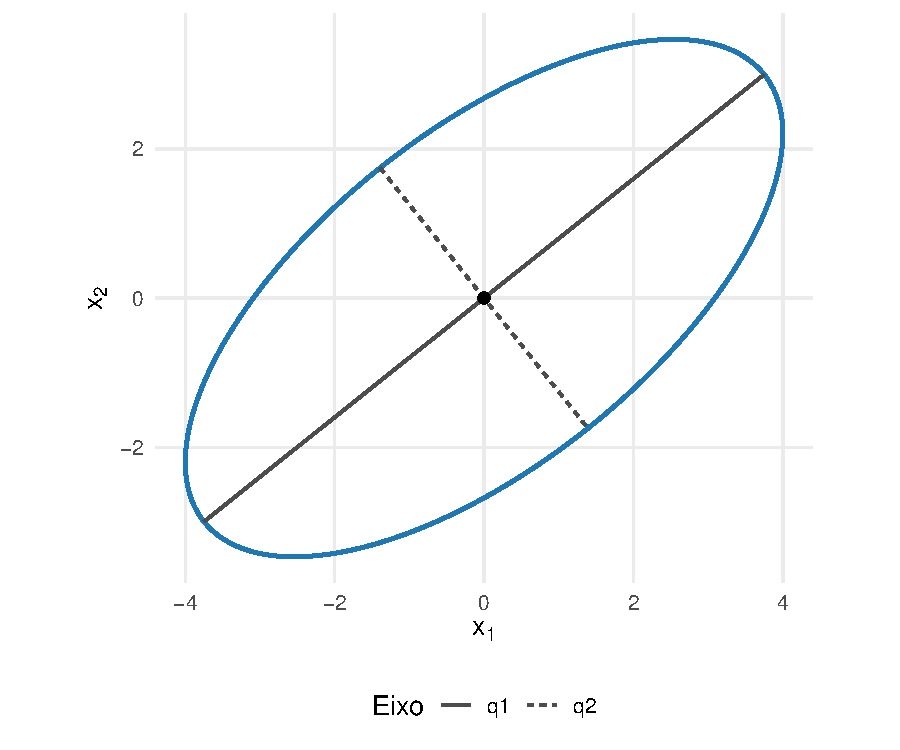
\includegraphics[keepaspectratio]{mod_2_covariancias_files/figure-pdf/fig-elipsoide-covariancia-1.pdf}}

}

\caption{\label{fig-elipsoide-covariancia}Elipse associada a uma matriz
de covariâncias e seus eixos espectrais.}

\end{figure}%

A orientação da elipse é determinada pelos autovetores, enquanto suas
extensões dependem das raízes quadradas dos autovalores. A matriz de
covariâncias determina, assim, uma geometria de segunda ordem para a
dispersão conjunta.

\begin{tcolorbox}[enhanced jigsaw, colback=white, breakable, bottomrule=.15mm, left=2mm, arc=.35mm, rightrule=.15mm, colframe=quarto-callout-caution-color-frame, toprule=.15mm, leftrule=.75mm, opacityback=0]

\vspace{-3mm}\textbf{Interpretação probabilística do elipsoide}\vspace{3mm}

O conjunto \(\mathcal E_c\) é definido somente por \(\boldsymbol{\mu}\)
e \(\boldsymbol{\Sigma}\). Sem uma hipótese adicional sobre a
distribuição de \(\boldsymbol{\mathsf X}\), não se pode atribuir a esse
elipsoide uma probabilidade específica nem interpretá-lo como região de
confiança. A interpretação probabilística dessas superfícies será
desenvolvida no Capítulo 9 para a distribuição normal multivariada.

\end{tcolorbox}

Quando \(\boldsymbol{\Sigma}\) é singular, a variabilidade está restrita
ao subespaço

\[
\mathcal C
\left(
\boldsymbol{\Sigma}
\right).
\]

A raiz quadrada principal definida na
Definição~\ref{def-raiz-quadrada-principal} permite representar o
elipsoide degenerado por

\begin{equation}\phantomsection\label{eq-elipsoide-covariancia-singular}{
\mathcal E_c^{(r)}
=
\left\{
\boldsymbol{\mu}
+
\boldsymbol{\Sigma}^{1/2}\mathbf u:
\|\mathbf u\|\leq c
\right\},
}\end{equation}

em que

\[
r
=
\operatorname{posto}
\left(
\boldsymbol{\Sigma}
\right)
<
p.
\]

Esse conjunto está contido no subespaço afim

\[
\boldsymbol{\mu}
+
\mathcal C
\left(
\boldsymbol{\Sigma}
\right)
\]

e possui \(r\) semieixos não nulos, com comprimentos
\(c\sqrt{\lambda_j}\) para os autovalores positivos. A pseudoinversa
será utilizada mais adiante para expressar a mesma geometria no contexto
da distância de Mahalanobis.

\subsection{Variância total, variância generalizada e
volume}\label{variuxe2ncia-total-variuxe2ncia-generalizada-e-volume}

Uma matriz de covariâncias contém toda a estrutura de segunda ordem do
vetor aleatório. Algumas funções escalares de \(\boldsymbol{\Sigma}\)
resumem aspectos específicos dessa dispersão, mas nenhuma delas
substitui a matriz completa.

\begin{definition}[Variância
total]\protect\hypertarget{def-variancia-total}{}\label{def-variancia-total}

Se \(\boldsymbol{\mathsf X}\in\mathbb R^p\) possui matriz de
covariâncias \(\boldsymbol{\Sigma}\), sua \textbf{variância total} é

\begin{equation}\phantomsection\label{eq-variancia-total}{
\operatorname{VT}
\left(
\boldsymbol{\mathsf X}
\right)
=
\operatorname{tr}
\left(
\boldsymbol{\Sigma}
\right).
}\end{equation}

\end{definition}

Pela definição de traço na Definição~\ref{def-traco},

\begin{equation}\phantomsection\label{eq-variancia-total-componentes}{
\operatorname{tr}
\left(
\boldsymbol{\Sigma}
\right)
=
\sum_{j=1}^p
\operatorname{Var}(X_j).
}\end{equation}

Pela decomposição espectral,

\begin{equation}\phantomsection\label{eq-variancia-total-autovalores}{
\operatorname{tr}
\left(
\boldsymbol{\Sigma}
\right)
=
\sum_{j=1}^p
\lambda_j.
}\end{equation}

A variância total também possui uma interpretação em termos de esperança
matemática. Mais geralmente, seja \(\mathbf A\in\mathbb{R}^{p\times p}\)
uma matriz simétrica e seja \(\mathbf a\in\mathbb{R}^p\) um vetor fixo.
Então,

\begin{equation}\phantomsection\label{eq-esperanca-forma-quadratica-geral}{
E
\left[
\left(
\boldsymbol{\mathsf X}
-
\mathbf a
\right)^\top
\mathbf A
\left(
\boldsymbol{\mathsf X}
-
\mathbf a
\right)
\right]
=
\operatorname{tr}
\left(
\mathbf A
\boldsymbol{\Sigma}
\right)
+
\left(
\boldsymbol{\mu}
-
\mathbf a
\right)^\top
\mathbf A
\left(
\boldsymbol{\mu}
-
\mathbf a
\right).
}\end{equation}

De fato,

\[
\boldsymbol{\mathsf X}
-
\mathbf a
=
\left(
\boldsymbol{\mathsf X}
-
\boldsymbol{\mu}
\right)
+
\left(
\boldsymbol{\mu}
-
\mathbf a
\right),
\]

e, ao expandir a forma quadrática, os termos cruzados possuem esperança
nula porque

\[
E
\left(
\boldsymbol{\mathsf X}
-
\boldsymbol{\mu}
\right)
=
\mathbf 0.
\]

Além disso,

\[
E
\left[
\left(
\boldsymbol{\mathsf X}
-
\boldsymbol{\mu}
\right)^\top
\mathbf A
\left(
\boldsymbol{\mathsf X}
-
\boldsymbol{\mu}
\right)
\right]
=
\operatorname{tr}
\left(
\mathbf A
\boldsymbol{\Sigma}
\right).
\]

Tomando

\[
\mathbf A
=
\mathbf I_p
\qquad
\text{e}
\qquad
\mathbf a
=
\boldsymbol{\mu},
\]

obtém-se

\begin{equation}\phantomsection\label{eq-variancia-total-distancia}{
E
\left[
\left\|
\boldsymbol{\mathsf X}
-
\boldsymbol{\mu}
\right\|^2
\right]
=
\operatorname{tr}
\left(
\boldsymbol{\Sigma}
\right).
}\end{equation}

Portanto, a variância total é o afastamento euclidiano quadrático médio
do vetor aleatório em relação ao seu vetor de médias.

Mais geralmente, tomando \(\mathbf A=\mathbf I_p\),

\begin{equation}\phantomsection\label{eq-esperanca-distancia-quadratica-ponto}{
E
\left[
\left\|
\boldsymbol{\mathsf X}
-
\mathbf a
\right\|^2
\right]
=
\operatorname{tr}
\left(
\boldsymbol{\Sigma}
\right)
+
\left\|
\boldsymbol{\mu}
-
\mathbf a
\right\|^2.
}\end{equation}

Essa expressão mostra que \(\boldsymbol{\mu}\) minimiza o afastamento
quadrático médio:

\[
E
\left[
\left\|
\boldsymbol{\mathsf X}
-
\mathbf a
\right\|^2
\right]
\geq
E
\left[
\left\|
\boldsymbol{\mathsf X}
-
\boldsymbol{\mu}
\right\|^2
\right].
\]

Como

\[
\operatorname{tr}
\left(
\boldsymbol{\Sigma}
\right)
=
\sum_{j=1}^p
\lambda_j,
\]

segue também que

\[
E
\left[
\left\|
\boldsymbol{\mathsf X}
-
\boldsymbol{\mu}
\right\|^2
\right]
=
\sum_{j=1}^p
\lambda_j.
\]

Assim, a mesma quantidade pode ser interpretada como soma das variâncias
marginais, soma das variâncias nos eixos espectrais ou afastamento
euclidiano quadrático médio em relação ao centro.

\begin{definition}[Variância
média]\protect\hypertarget{def-variancia-media}{}\label{def-variancia-media}

Se \(\boldsymbol{\mathsf X}\in\mathbb R^p\) possui matriz de
covariâncias \(\boldsymbol{\Sigma}\), com autovalores
\(\lambda_1,\ldots,\lambda_p\), sua \textbf{variância média} é

\[
\operatorname{VM}
\left(
\boldsymbol{\mathsf X}
\right)
=
\frac{1}{p}
\operatorname{tr}
\left(
\boldsymbol{\Sigma}
\right)
=
\frac{1}{p}
\sum_{j=1}^p
\lambda_j.
\]

\end{definition}

A variância total e a variância média dependem das escalas das
componentes. Quando as variáveis possuem unidades distintas, sua
interpretação requer cautela.

Outra medida utiliza o determinante da matriz de covariâncias.

\begin{definition}[Variância
generalizada]\protect\hypertarget{def-variancia-generalizada}{}\label{def-variancia-generalizada}

Se \(\boldsymbol{\mathsf X}\in\mathbb R^p\) possui matriz de
covariâncias \(\boldsymbol{\Sigma}\), sua \textbf{variância
generalizada} é

\begin{equation}\phantomsection\label{eq-variancia-generalizada}{
\operatorname{VG}
\left(
\boldsymbol{\mathsf X}
\right)
=
\det
\left(
\boldsymbol{\Sigma}
\right).
}\end{equation}

\end{definition}

Pelas propriedades do determinante e pela decomposição espectral,

\begin{equation}\phantomsection\label{eq-variancia-generalizada-autovalores}{
\det
\left(
\boldsymbol{\Sigma}
\right)
=
\prod_{j=1}^p
\lambda_j.
}\end{equation}

A variância generalizada reúne multiplicativamente as dispersões nos
eixos espectrais. Se pelo menos um autovalor é zero,

\[
\det
\left(
\boldsymbol{\Sigma}
\right)
=
0,
\]

mesmo que exista variabilidade nas demais direções. Nesse caso, o valor
zero indica que a dispersão ocupa um subespaço de dimensão inferior a
\(p\); não indica ausência de variabilidade.

A variância generalizada não deve ser confundida com o volume do
elipsoide de covariância. A relação entre as duas quantidades envolve a
raiz quadrada do determinante (Johnson; Wichern, 2007).

\begin{proposition}[Volume do elipsoide de
covariância]\protect\hypertarget{prp-volume-elipsoide-covariancia}{}\label{prp-volume-elipsoide-covariancia}

Se

\[
p\geq1,
\qquad
\boldsymbol{\mu}\in\mathbb R^p,
\qquad
\boldsymbol{\Sigma}\in\mathbb R^{p\times p},
\qquad
\boldsymbol{\Sigma}\succ\mathbf0
\]

e

\[
c>0,
\]

considere o elipsoide

\[
\mathcal E_c
=
\left\{
\mathbf x\in\mathbb R^p:
\left(
\mathbf x-\boldsymbol{\mu}
\right)^\top
\boldsymbol{\Sigma}^{-1}
\left(
\mathbf x-\boldsymbol{\mu}
\right)
\leq
c^2
\right\}.
\]

Seu volume \(p\)-dimensional é

\begin{equation}\phantomsection\label{eq-volume-elipsoide-covariancia}{
\operatorname{Vol}_p
\left(
\mathcal E_c
\right)
=
\kappa_p
c^p
\det
\left(
\boldsymbol{\Sigma}
\right)^{1/2},
}\end{equation}

em que

\[
\kappa_p
=
\frac{
\pi^{p/2}
}{
\Gamma
\left(
p/2+1
\right)
}
\]

é o volume da esfera unitária de \(\mathbb{R}^p\).

\end{proposition}

\begin{proof}
O elipsoide é a imagem da bola

\[
\mathcal B_c
=
\left\{
\mathbf u\in\mathbb{R}^p:
\|\mathbf u\|\leq c
\right\}
\]

pela transformação

\[
\mathbf x
=
\boldsymbol{\mu}
+
\boldsymbol{\Sigma}^{1/2}\mathbf u.
\]

A translação não altera o volume. Pelo
Proposição~\ref{prp-determinante-volume-transformacao}, a transformação
linear multiplica volumes por

\[
\left|
\det
\left(
\boldsymbol{\Sigma}^{1/2}
\right)
\right|
=
\det
\left(
\boldsymbol{\Sigma}
\right)^{1/2}.
\]

Como

\[
\operatorname{Vol}_p
\left(
\mathcal B_c
\right)
=
\kappa_pc^p,
\]

obtém-se Equação~\ref{eq-volume-elipsoide-covariancia}.
\end{proof}

Portanto,

\[
\det
\left(
\boldsymbol{\Sigma}
\right)^{1/2}
\]

é o fator associado à escala de volume da dispersão, enquanto

\[
\det
\left(
\boldsymbol{\Sigma}
\right)
\]

é a variância generalizada.

\begin{example}[Variância total e variância
generalizada]\protect\hypertarget{exm-medidas-globais-dispersao}{}\label{exm-medidas-globais-dispersao}

Considere

\[
\boldsymbol{\Sigma}_1
=
\begin{bmatrix}
4 & 0\\
0 & 4
\end{bmatrix}
\]

e

\[
\boldsymbol{\Sigma}_2
=
\begin{bmatrix}
7 & 0\\
0 & 1
\end{bmatrix}.
\]

As duas matrizes possuem a mesma variância total:

\[
\operatorname{tr}
\left(
\boldsymbol{\Sigma}_1
\right)
=
\operatorname{tr}
\left(
\boldsymbol{\Sigma}_2
\right)
=
8.
\]

Entretanto,

\[
\det
\left(
\boldsymbol{\Sigma}_1
\right)
=
16
\]

e

\[
\det
\left(
\boldsymbol{\Sigma}_2
\right)
=
7.
\]

A primeira configuração distribui a variabilidade igualmente entre os
dois eixos. A segunda concentra maior variabilidade em uma direção e
menor variabilidade na outra. A igualdade das variâncias totais não
implica, portanto, igualdade da geometria da dispersão.

\end{example}

As unidades também diferem entre essas medidas. Se as componentes
possuem unidades

\[
u_1,\ldots,u_p,
\]

a variância generalizada possui unidade

\[
u_1^2\cdots u_p^2,
\]

enquanto

\[
\det
\left(
\boldsymbol{\Sigma}
\right)^{1/2}
\]

possui unidade

\[
u_1\cdots u_p,
\]

compatível com uma medida de volume no espaço das variáveis.

Considere agora uma transformação linear quadrada

\[
\boldsymbol{\mathsf Y}
=
\mathbf A
\boldsymbol{\mathsf X},
\qquad
\mathbf A
\in
\mathbb{R}^{p\times p}.
\]

Pela expressão Equação~\ref{eq-covariancia-transformacao-afim},

\[
\boldsymbol{\Sigma}_{YY}
=
\mathbf A
\boldsymbol{\Sigma}_{XX}
\mathbf A^\top.
\]

Consequentemente,

\begin{equation}\phantomsection\label{eq-variancia-generalizada-transformacao}{
\det
\left(
\boldsymbol{\Sigma}_{YY}
\right)
=
\det(\mathbf A)^2
\det
\left(
\boldsymbol{\Sigma}_{XX}
\right).
}\end{equation}

Para a escala de volume,

\begin{equation}\phantomsection\label{eq-raiz-variancia-generalizada-transformacao}{
\det
\left(
\boldsymbol{\Sigma}_{YY}
\right)^{1/2}
=
|\det(\mathbf A)|
\det
\left(
\boldsymbol{\Sigma}_{XX}
\right)^{1/2}.
}\end{equation}

Essa expressão é compatível com o fator de alteração de volume
desenvolvido na Proposição~\ref{prp-determinante-volume-transformacao}.

Quando \(\mathbf A\) é ortogonal, \(|\det(\mathbf A)|=1\) e a
transformação preserva os autovalores de \(\boldsymbol{\Sigma}\).
Consequentemente, preserva a variância total, a variância generalizada e
os comprimentos dos semieixos do elipsoide, alterando somente sua
orientação no sistema de coordenadas.

A forma quadrática que define o elipsoide fornece também uma medida de
afastamento adaptada à estrutura de covariâncias. Essa medida é a
distância de Mahalanobis.

\section{Distância de Mahalanobis}\label{distuxe2ncia-de-mahalanobis}

A distância euclidiana utiliza a mesma geometria em todas as direções.
Em dados multivariados, entretanto, um deslocamento pode representar um
afastamento pequeno em uma direção de grande variabilidade e um
afastamento expressivo em outra direção de pequena variabilidade.

A distância de Mahalanobis incorpora essa estrutura por meio da matriz
de covariâncias. No caso univariado, ela reduz o afastamento \(|x-\mu|\)
à sua escala natural,

\[
\frac{|x-\mu|}{\sigma}.
\]

\begin{definition}[Distância de
Mahalanobis]\protect\hypertarget{def-distancia-mahalanobis}{}\label{def-distancia-mahalanobis}

Se \(\boldsymbol{\Sigma}\in\mathbb R^{p\times p}\) é positiva definida,
a \textbf{distância de Mahalanobis} entre
\(\mathbf x,\mathbf y\in\mathbb{R}^p\), em relação a
\(\boldsymbol{\Sigma}\), é

\begin{equation}\phantomsection\label{eq-distancia-mahalanobis-dois-pontos}{
d_M
\left(
\mathbf x,
\mathbf y;
\boldsymbol{\Sigma}
\right)
=
\sqrt{
\left(
\mathbf x-\mathbf y
\right)^\top
\boldsymbol{\Sigma}^{-1}
\left(
\mathbf x-\mathbf y
\right)
}.
}\end{equation}

Em particular, a distância de \(\mathbf x\) ao vetor de médias é

\begin{equation}\phantomsection\label{eq-distancia-mahalanobis-centro}{
d_M
\left(
\mathbf x,
\boldsymbol{\mu}
\right)
=
\sqrt{
\left(
\mathbf x-\boldsymbol{\mu}
\right)^\top
\boldsymbol{\Sigma}^{-1}
\left(
\mathbf x-\boldsymbol{\mu}
\right)
}.
}\end{equation}

\end{definition}

\subsection{Interpretação geométrica e
espectral}\label{interpretauxe7uxe3o-geomuxe9trica-e-espectral}

O quadrado da distância de Mahalanobis de \(\mathbf x\) ao vetor de
médias é

\begin{equation}\phantomsection\label{eq-distancia-quadratica-mahalanobis}{
d_M^2
\left(
\mathbf x,
\boldsymbol{\mu}
\right)
=
\left(
\mathbf x-\boldsymbol{\mu}
\right)^\top
\boldsymbol{\Sigma}^{-1}
\left(
\mathbf x-\boldsymbol{\mu}
\right).
}\end{equation}

Como \(\boldsymbol{\Sigma}^{-1}\succ\mathbf 0\), ela define o produto
interno induzido apresentado na
Definição~\ref{def-produto-interno-induzido} e a norma correspondente de
Definição~\ref{def-norma-induzida}. Assim,
Equação~\ref{eq-distancia-mahalanobis-dois-pontos} é uma distância
métrica, sem necessidade de repetir aqui a demonstração das propriedades
métricas desenvolvidas no Módulo 1.

Quando

\[
\boldsymbol{\Sigma}
=
\mathbf I_p,
\]

a distância de Mahalanobis coincide com a distância euclidiana. Quando
\(p=1\),

\[
d_M(x,\mu)
=
\frac{|x-\mu|}{\sigma}.
\]

A medida é adimensional, pois a inversa da matriz de covariâncias
compensa as unidades presentes no vetor de diferenças.

A interpretação espectral decorre diretamente de
Equação~\ref{eq-decomposicao-espectral-covariancia}. Se

\[
\mathbf u
=
\mathbf Q^\top
\left(
\mathbf x-\boldsymbol{\mu}
\right),
\]

então

\begin{equation}\phantomsection\label{eq-mahalanobis-eixos-espectrais}{
d_M^2
\left(
\mathbf x,
\boldsymbol{\mu}
\right)
=
\sum_{j=1}^p
\frac{
u_j^2
}{
\lambda_j
}.
}\end{equation}

Essa expressão mostra como a distância de Mahalanobis incorpora a
geometria da dispersão. Cada componente \(u_j\) representa o
deslocamento de \(\mathbf x-\boldsymbol{\mu}\) na direção do autovetor
correspondente, enquanto \(\lambda_j\) é a variância nessa direção.

Cada deslocamento é, portanto, ponderado pelo inverso da variância na
direção correspondente. Um mesmo deslocamento geométrico recebe menor
peso em uma direção de grande variabilidade e maior peso em uma direção
de pequena variabilidade.

\begin{example}[Afastamentos em direções com variâncias
distintas]\protect\hypertarget{exm-mahalanobis-eixos-espectrais}{}\label{exm-mahalanobis-eixos-espectrais}

Considere dois eixos espectrais com

\[
\lambda_1
=
9
\qquad
\text{e}
\qquad
\lambda_2
=
1.
\]

Um afastamento de magnitude \(2\) ao longo do primeiro eixo produz

\[
d_M^2
=
\frac{2^2}{9}
=
\frac{4}{9}.
\]

O mesmo afastamento ao longo do segundo produz

\[
d_M^2
=
\frac{2^2}{1}
=
4.
\]

Os dois pontos possuem a mesma distância euclidiana ao centro, mas o
segundo apresenta maior distância de Mahalanobis porque se encontra em
uma direção com menor dispersão populacional.

\end{example}

As superfícies de igual distância,

\[
d_M
\left(
\mathbf x,
\boldsymbol{\mu}
\right)
=
c,
\]

são exatamente as fronteiras dos elipsoides definidos na
Equação~\ref{eq-elipsoide-covariancia}. Isso reforça a interpretação
geométrica da distância de Mahalanobis: pontos pertencentes à mesma
superfície elipsoidal apresentam o mesmo afastamento em relação ao
centro quando a estrutura de covariâncias é considerada.

A Figura~\ref{fig-distancia-mahalanobis} compara dois deslocamentos com
a mesma distância euclidiana ao centro, mas orientados segundo eixos de
dispersão distintos.

\begin{figure}

\centering{

\pandocbounded{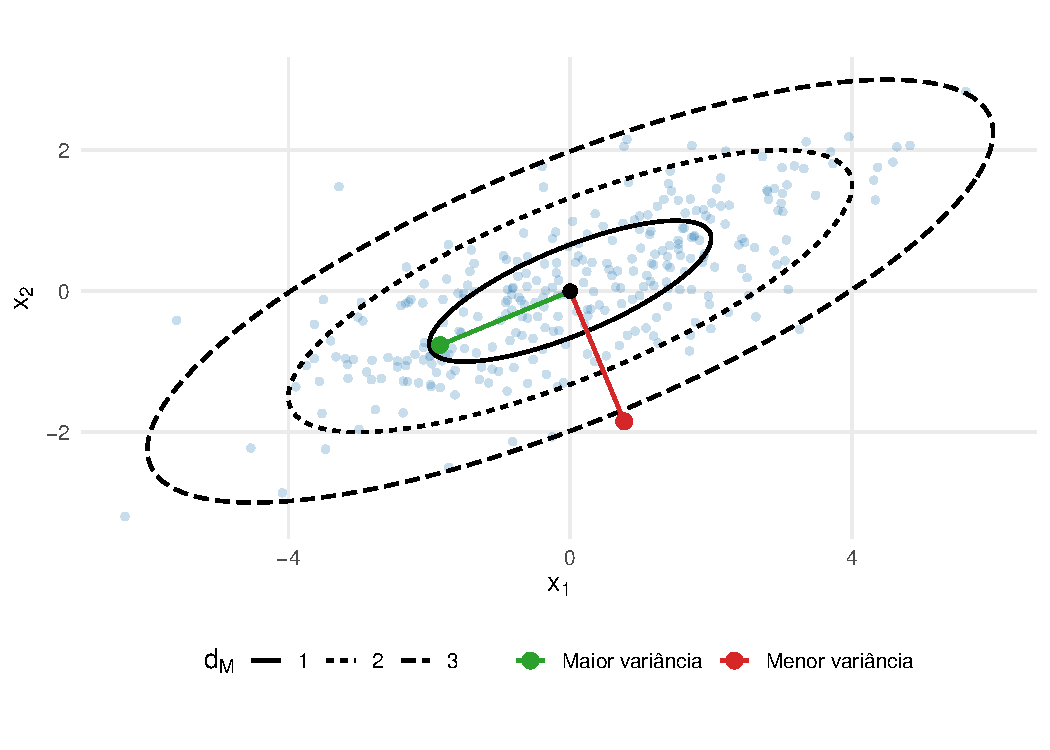
\includegraphics[keepaspectratio]{mod_2_covariancias_files/figure-pdf/fig-distancia-mahalanobis-1.pdf}}

}

\caption{\label{fig-distancia-mahalanobis}Pontos com a mesma distância
euclidiana podem apresentar distâncias de Mahalanobis distintas.}

\end{figure}%

O ponto situado no eixo de menor variância pertence a uma curva de maior
distância de Mahalanobis. A medida compara o deslocamento com a
quantidade de variabilidade disponível na direção em que ele ocorre.

\subsection{Branqueamento e
esferização}\label{branqueamento-e-esferizauxe7uxe3o}

Uma forma alternativa de compreender a geometria associada à matriz de
covariâncias consiste em transformar as coordenadas de modo que a
variabilidade resultante seja a mesma em todas as direções.

Seja \(\boldsymbol{\mathsf X}\) um vetor aleatório com vetor de médias
\(\boldsymbol{\mu}\) e matriz de covariâncias
\(\boldsymbol{\Sigma}\succ\mathbf 0\). Uma transformação linear da forma

\[
\boldsymbol{\mathsf Z}
=
\mathbf W
\left(
\boldsymbol{\mathsf X}
-
\boldsymbol{\mu}
\right)
\]

é denominada \textbf{branqueamento} (\emph{whitening}) quando a matriz
\(\mathbf W\) é escolhida de modo que

\[
\operatorname{Cov}
\left(
\boldsymbol{\mathsf Z}
\right)
=
\mathbf W
\boldsymbol{\Sigma}
\mathbf W^\top
=
\mathbf I_p.
\]

Assim, as componentes do vetor branqueado possuem variância unitária e
covariâncias nulas entre si. O termo \textbf{esferização} enfatiza a
interpretação geométrica da mesma transformação: os elipsoides
associados à estrutura de covariâncias são transformados em esferas.

Essa interpretação refere-se à estrutura de segunda ordem do vetor
aleatório, representada pela matriz de covariâncias. Em geral, o
branqueamento não implica que toda a distribuição do vetor transformado
seja esfericamente simétrica.

A raiz quadrada inversa de uma matriz positiva definida foi construída
no Capítulo 5 a partir da raiz quadrada principal dada na
Definição~\ref{def-raiz-quadrada-principal}. Uma escolha para a matriz
de branqueamento é

\[
\mathbf W
=
\boldsymbol{\Sigma}^{-1/2},
\]

pois

\[
\boldsymbol{\Sigma}^{-1/2}
\boldsymbol{\Sigma}
\boldsymbol{\Sigma}^{-1/2}
=
\mathbf I_p.
\] Essa escolha é denominada \textbf{branqueamento simétrico}. Ela
remove simultaneamente as diferenças de variância e as covariâncias
entre as componentes. Para um ponto \(\mathbf x\), a transformação
correspondente é

\begin{equation}\phantomsection\label{eq-transformacao-branqueamento-ponto}{
\mathbf z
=
\boldsymbol{\Sigma}^{-1/2}
\left(
\mathbf x-\boldsymbol{\mu}
\right).
}\end{equation}

Para o vetor aleatório,

\[
\boldsymbol{\mathsf Z}
=
\boldsymbol{\Sigma}^{-1/2}
\left(
\boldsymbol{\mathsf X}
-
\boldsymbol{\mu}
\right),
\]

tem-se

\begin{equation}\phantomsection\label{eq-covariancia-vetor-branqueado}{
E
\left(
\boldsymbol{\mathsf Z}
\right)
=
\mathbf 0
\qquad
\text{e}
\qquad
\operatorname{Cov}
\left(
\boldsymbol{\mathsf Z}
\right)
=
\mathbf I_p.
}\end{equation}

A transformação de branqueamento também permite interpretar diretamente
a distância de Mahalanobis. De
Equação~\ref{eq-transformacao-branqueamento-ponto},

\[
\begin{aligned}
\|\mathbf z\|^2
&=
\left(
\mathbf x-\boldsymbol{\mu}
\right)^\top
\boldsymbol{\Sigma}^{-1}
\left(
\mathbf x-\boldsymbol{\mu}
\right)\\
&=
d_M^2
\left(
\mathbf x,
\boldsymbol{\mu}
\right).
\end{aligned}
\]

Logo,

\begin{equation}\phantomsection\label{eq-mahalanobis-distancia-euclidiana-transformada}{
d_M
\left(
\mathbf x,
\boldsymbol{\mu}
\right)
=
\left\|
\boldsymbol{\Sigma}^{-1/2}
\left(
\mathbf x-\boldsymbol{\mu}
\right)
\right\|.
}\end{equation}

A distância de Mahalanobis é, portanto, a distância euclidiana após a
centralização e o branqueamento.

A esperança da distância quadrática de Mahalanobis também depende apenas
da matriz de covariâncias. Como

\[
d_M^2
\left(
\boldsymbol{\mathsf X},
\boldsymbol{\mu}
\right)
=
\left(
\boldsymbol{\mathsf X}
-
\boldsymbol{\mu}
\right)^\top
\boldsymbol{\Sigma}^{-1}
\left(
\boldsymbol{\mathsf X}
-
\boldsymbol{\mu}
\right),
\]

a expressão Equação~\ref{eq-esperanca-forma-quadratica-geral}, com

\[
\mathbf A
=
\boldsymbol{\Sigma}^{-1},
\]

fornece

\begin{equation}\phantomsection\label{eq-esperanca-mahalanobis-quadratica}{
\begin{aligned}
E
\left[
d_M^2
\left(
\boldsymbol{\mathsf X},
\boldsymbol{\mu}
\right)
\right]
&=
\operatorname{tr}
\left(
\boldsymbol{\Sigma}^{-1}
\boldsymbol{\Sigma}
\right)\\
&=
\operatorname{tr}
\left(
\mathbf I_p
\right)\\
&=
p.
\end{aligned}
}\end{equation}

Esse resultado utiliza apenas a existência de \(\boldsymbol{\mu}\) e
\(\boldsymbol{\Sigma}\succ\mathbf 0\); não requer normalidade. No
Capítulo 9, a hipótese de normalidade multivariada permitirá
caracterizar não apenas essa esperança, mas a distribuição completa da
distância quadrática de Mahalanobis.

\begin{example}[Branqueamento a partir da decomposição
espectral]\protect\hypertarget{exm-branqueamento-espectral-covariancia}{}\label{exm-branqueamento-espectral-covariancia}

Retome a matriz de covariâncias do
Exemplo~\ref{exm-variancias-eixos-espectrais},

\[
\boldsymbol{\Sigma}
=
\begin{bmatrix}
4 & 2\\
2 & 4
\end{bmatrix}.
\]

Sua decomposição espectral é

\[
\boldsymbol{\Sigma}
=
\mathbf Q
\boldsymbol{\Lambda}
\mathbf Q^\top,
\]

com

\[
\mathbf Q
=
\frac{1}{\sqrt{2}}
\begin{bmatrix}
1 & 1\\
1 & -1
\end{bmatrix}
\]

e

\[
\boldsymbol{\Lambda}
=
\begin{bmatrix}
6 & 0\\
0 & 2
\end{bmatrix}.
\]

Utilizando a raiz quadrada inversa desenvolvida no Módulo 1,

\[
\boldsymbol{\Sigma}^{-1/2}
=
\mathbf Q
\boldsymbol{\Lambda}^{-1/2}
\mathbf Q^\top,
\]

em que

\[
\boldsymbol{\Lambda}^{-1/2}
=
\begin{bmatrix}
1/\sqrt{6} & 0\\
0 & 1/\sqrt{2}
\end{bmatrix}.
\]

Defina

\[
\boldsymbol{\mathsf Z}
=
\boldsymbol{\Sigma}^{-1/2}
\left(
\boldsymbol{\mathsf X}
-
\boldsymbol{\mu}
\right).
\]

Então,

\[
\begin{aligned}
\operatorname{Cov}
\left(
\boldsymbol{\mathsf Z}
\right)
&=
\boldsymbol{\Sigma}^{-1/2}
\boldsymbol{\Sigma}
\boldsymbol{\Sigma}^{-1/2}\\
&=
\mathbf Q
\boldsymbol{\Lambda}^{-1/2}
\mathbf Q^\top
\mathbf Q
\boldsymbol{\Lambda}
\mathbf Q^\top
\mathbf Q
\boldsymbol{\Lambda}^{-1/2}
\mathbf Q^\top\\
&=
\mathbf Q
\boldsymbol{\Lambda}^{-1/2}
\boldsymbol{\Lambda}
\boldsymbol{\Lambda}^{-1/2}
\mathbf Q^\top\\
&=
\mathbf Q
\mathbf I_2
\mathbf Q^\top\\
&=
\mathbf I_2.
\end{aligned}
\]

A transformação pode ser compreendida em três etapas:

\[
\boldsymbol{\mathsf X}
-
\boldsymbol{\mu}
\quad
\xrightarrow{\ \mathbf Q^\top\ }
\quad
\text{coordenadas nos eixos espectrais}
\]

\[
\xrightarrow{\ \boldsymbol{\Lambda}^{-1/2}\ }
\quad
\text{reescalonamento para variância unitária}
\]

\[
\xrightarrow{\ \mathbf Q\ }
\quad
\boldsymbol{\mathsf Z}.
\]

O primeiro passo expressa o vetor na base de autovetores de
\(\boldsymbol{\Sigma}\), na qual a matriz de covariâncias é diagonal. O
segundo divide cada coordenada por \(\sqrt{\lambda_j}\), tornando todas
as variâncias iguais a \(1\). O terceiro retorna ao sistema original de
coordenadas por meio da transformação ortogonal \(\mathbf Q\).

Considere agora um ponto cuja diferença em relação ao centro é

\[
\mathbf x
-
\boldsymbol{\mu}
=
\begin{bmatrix}
2\\
0
\end{bmatrix}.
\]

Suas coordenadas espectrais são

\[
\mathbf Q^\top
\left(
\mathbf x-\boldsymbol{\mu}
\right)
=
\begin{bmatrix}
\sqrt{2}\\
\sqrt{2}
\end{bmatrix}.
\]

Pela expressão Equação~\ref{eq-mahalanobis-eixos-espectrais},

\[
\begin{aligned}
d_M^2
\left(
\mathbf x,
\boldsymbol{\mu}
\right)
&=
\frac{
(\sqrt{2})^2
}{6}
+
\frac{
(\sqrt{2})^2
}{2}\\
&=
\frac{2}{6}
+
\frac{2}{2}\\
&=
\frac{4}{3}.
\end{aligned}
\]

Por outro lado,

\[
\left\|
\boldsymbol{\Sigma}^{-1/2}
\left(
\mathbf x-\boldsymbol{\mu}
\right)
\right\|^2
=
\frac{4}{3}.
\]

Assim, o exemplo verifica concretamente a identidade

\[
d_M
\left(
\mathbf x,
\boldsymbol{\mu}
\right)
=
\left\|
\boldsymbol{\Sigma}^{-1/2}
\left(
\mathbf x-\boldsymbol{\mu}
\right)
\right\|.
\]

A decomposição espectral, a raiz matricial, o branqueamento e a
distância de Mahalanobis aparecem, portanto, como partes de uma mesma
construção geométrica.

\end{example}

O branqueamento não é único. De fato, se \(\mathbf Q_0\) é uma matriz
ortogonal, então

\[
\mathbf W
=
\mathbf Q_0
\boldsymbol{\Sigma}^{-1/2}
\]

também satisfaz

\[
\mathbf W
\boldsymbol{\Sigma}
\mathbf W^\top
=
\mathbf I_p.
\]

Portanto, diferentes transformações podem produzir vetores com matriz de
covariâncias igual à identidade. Essas versões diferem por uma
transformação ortogonal e, consequentemente, preservam as distâncias
euclidianas no espaço branqueado.

A padronização marginal e o branqueamento devem ser distinguidos. Pela
expressão Equação~\ref{eq-matriz-correlacoes-populacional}, a
padronização marginal produz

\[
\operatorname{Cov}
\left(
\mathbf D_{\Sigma}^{-1/2}
\left(
\boldsymbol{\mathsf X}
-
\boldsymbol{\mu}
\right)
\right)
=
\boldsymbol{\mathcal R}.
\]

Assim, a padronização marginal torna as variâncias iguais a \(1\), mas a
matriz resultante pode apresentar correlações não nulas fora da
diagonal. O branqueamento, por sua vez, utiliza a estrutura completa da
matriz de covariâncias e produz

\[
\operatorname{Cov}
\left(
\boldsymbol{\mathsf Z}
\right)
=
\mathbf I_p.
\]

Se

\[
\mathbf z_D
=
\mathbf D_{\Sigma}^{-1/2}
\left(
\mathbf x-\boldsymbol{\mu}
\right),
\]

a relação

\[
\boldsymbol{\Sigma}
=
\mathbf D_{\Sigma}^{1/2}
\boldsymbol{\mathcal R}
\mathbf D_{\Sigma}^{1/2}
\]

implica

\begin{equation}\phantomsection\label{eq-mahalanobis-correlacao}{
d_M^2
\left(
\mathbf x,
\boldsymbol{\mu}
\right)
=
\mathbf z_D^\top
\boldsymbol{\mathcal R}^{-1}
\mathbf z_D.
}\end{equation}

Assim, a padronização marginal remove as escalas individuais, enquanto
\(\boldsymbol{\mathcal R}^{-1}\) incorpora a associação linear
remanescente. Somente quando

\[
\boldsymbol{\mathcal R}
=
\mathbf I_p
\]

a distância de Mahalanobis coincide com a distância euclidiana entre as
coordenadas marginalmente padronizadas.

\section{Representação descritiva a partir dos
dados}\label{representauxe7uxe3o-descritiva-a-partir-dos-dados}

As matrizes \(\boldsymbol{\Sigma}\) e \(\boldsymbol{\mathcal R}\) são
objetos populacionais. Quando se dispõe de um conjunto de dados
observado, a localização e a dispersão conjunta podem ser representadas
por quantidades calculadas diretamente a partir das observações.

Nesta seção,

\[
\bar{\mathbf x},
\qquad
\mathbf S
\qquad
\text{e}
\qquad
\mathbf R
\]

representam valores obtidos de uma matriz de dados específica. Quando as
linhas dessa matriz forem consideradas realizações de uma amostra
aleatória, esses valores corresponderão a realizações das estatísticas

\[
\bar{\boldsymbol{\mathsf X}},
\qquad
\boldsymbol{\mathsf S}
\qquad
\text{e}
\qquad
\boldsymbol{\mathsf R}.
\]

As propriedades dessas estatísticas como estimadores serão desenvolvidas
no Capítulo 10.

\subsection{Centralização, SQPC e matriz de covariâncias
observada}\label{centralizauxe7uxe3o-sqpc-e-matriz-de-covariuxe2ncias-observada}

Considere \(n\geq2\) observações de \(p\) variáveis organizadas,
conforme Definição~\ref{def-matriz-dados}, em

\[
\mathbf X
=
\begin{bmatrix}
\mathbf x_1^\top\\
\mathbf x_2^\top\\
\vdots\\
\mathbf x_n^\top
\end{bmatrix}
\in
\mathbb{R}^{n\times p},
\]

em que

\[
\mathbf x_i
\in
\mathbb{R}^p
\]

representa a \(i\)-ésima observação.

O vetor de médias das colunas é

\begin{equation}\phantomsection\label{eq-media-observada-matricial}{
\bar{\mathbf x}
=
\frac{1}{n}
\mathbf X^\top
\mathbf 1_n
\in
\mathbb{R}^p,
}\end{equation}

em que

\[
\mathbf 1_n
=
(1,\ldots,1)^\top
\in
\mathbb{R}^n.
\]

A matriz de dados centralizada é

\begin{equation}\phantomsection\label{eq-matriz-dados-centralizada}{
\mathbf X_c
=
\mathbf X
-
\mathbf 1_n
\bar{\mathbf x}^{\top}.
}\end{equation}

Cada linha de \(\mathbf X_c\) é

\[
\left(
\mathbf x_i
-
\bar{\mathbf x}
\right)^\top,
\]

e suas colunas satisfazem

\begin{equation}\phantomsection\label{eq-soma-colunas-centralizadas}{
\mathbf 1_n^\top
\mathbf X_c
=
\mathbf 0^\top.
}\end{equation}

Retomando a matriz de centralização utilizada no Capítulo 4,

\[
\mathbf H_n
=
\mathbf I_n
-
\frac{1}{n}
\mathbf 1_n
\mathbf 1_n^\top,
\]

tem-se

\begin{equation}\phantomsection\label{eq-centralizacao-por-hn}{
\mathbf X_c
=
\mathbf H_n
\mathbf X.
}\end{equation}

A operação remove a localização das colunas sem alterar as diferenças
entre as observações, conforme a propriedade estabelecida na
Proposição~\ref{prp-centralizacao-preserva-distancias}.

\begin{definition}[Matriz total de somas de quadrados e produtos
cruzados]\protect\hypertarget{def-matriz-sscp-total}{}\label{def-matriz-sscp-total}

A \textbf{matriz total de somas de quadrados e produtos cruzados}, ou
matriz total SQPC, é

\[
\mathbf T
=
\sum_{i=1}^n
\left(
\mathbf x_i
-
\bar{\mathbf x}
\right)
\left(
\mathbf x_i
-
\bar{\mathbf x}
\right)^\top.
\]

Equivalentemente,

\begin{equation}\phantomsection\label{eq-definicao-sscp-total}{
\mathbf T
=
\mathbf X_c^\top
\mathbf X_c
=
\mathbf X^\top
\mathbf H_n
\mathbf X.
}\end{equation}

\end{definition}

A sigla \textbf{SQPC} significa \textbf{Somas de Quadrados e Produtos
Cruzados} e será utilizada como equivalente, em português, à sigla
inglesa \textbf{SSCP}, de \emph{sum of squares and cross-products}. O
elemento \((j,k)\) de \(\mathbf T\) é

\[
t_{jk}
=
\sum_{i=1}^n
\left(
x_{ij}
-
\bar{x}_j
\right)
\left(
x_{ik}
-
\bar{x}_k
\right).
\]

Quando \(j=k\), \(t_{jj}\) é a soma dos quadrados dos desvios da
variável \(j\). Quando \(j\neq k\), \(t_{jk}\) é a soma dos produtos
cruzados entre as variáveis \(j\) e \(k\).

Como

\[
\mathbf T
=
\mathbf X_c^\top
\mathbf X_c,
\]

ela é uma matriz de Gram das colunas centralizadas no sentido de
Definição~\ref{def-matriz-gram}. Assim, pelas propriedades estabelecidas
na Proposição~\ref{prp-propriedades-matriz-gram},

\[
\mathbf T
=
\mathbf T^\top,
\]

\[
\mathbf T
\succeq
\mathbf 0
\]

e

\[
\operatorname{posto}
\left(
\mathbf T
\right)
=
\operatorname{posto}
\left(
\mathbf X_c
\right).
\]

A centralização impõe

\[
\mathbf 1_n^\top
\mathbf X_c
=
\mathbf 0^\top,
\]

de modo que as colunas de \(\mathbf X_c\) pertencem ao subespaço
ortogonal a \(\mathbf 1_n\), cuja dimensão é \(n-1\). Consequentemente,

\begin{equation}\phantomsection\label{eq-posto-sscp-total}{
\operatorname{posto}
\left(
\mathbf T
\right)
=
\operatorname{posto}
\left(
\mathbf X_c
\right)
\leq
\min(p,n-1).
}\end{equation}

A matriz \(\mathbf T\) registra a dispersão sem uma normalização pelo
número de observações.

\begin{definition}[Matriz de covariâncias
observada]\protect\hypertarget{def-matriz-covariancias-observada}{}\label{def-matriz-covariancias-observada}

A \textbf{matriz de covariâncias observada} é

\[
\mathbf S
=
\frac{1}{n-1}
\mathbf T.
\]

Equivalentemente,

\begin{equation}\phantomsection\label{eq-matriz-covariancias-observada}{
\mathbf S
=
\frac{1}{n-1}
\mathbf X_c^\top
\mathbf X_c
=
\frac{1}{n-1}
\mathbf X^\top
\mathbf H_n
\mathbf X.
}\end{equation}

\end{definition}

Seu elemento \((j,k)\) é

\begin{equation}\phantomsection\label{eq-elemento-covariancia-observada}{
s_{jk}
=
\frac{1}{n-1}
\sum_{i=1}^n
\left(
x_{ij}
-
\bar{x}_j
\right)
\left(
x_{ik}
-
\bar{x}_k
\right).
}\end{equation}

Os elementos diagonais são as variâncias calculadas para as colunas,

\[
s_{jj}
=
\frac{1}{n-1}
\sum_{i=1}^n
\left(
x_{ij}
-
\bar{x}_j
\right)^2,
\]

e os elementos fora da diagonal são as covariâncias calculadas entre
pares de colunas.

Como \(\mathbf S\) é um múltiplo positivo de \(\mathbf T\),

\[
\mathbf S
=
\mathbf S^\top,
\qquad
\mathbf S
\succeq
\mathbf 0
\]

e

\[
\operatorname{posto}
\left(
\mathbf S
\right)
=
\operatorname{posto}
\left(
\mathbf T
\right)
=
\operatorname{posto}
\left(
\mathbf X_c
\right).
\]

Portanto,

\begin{equation}\phantomsection\label{eq-posto-covariancia-observada}{
\operatorname{posto}
\left(
\mathbf S
\right)
\leq
\min(p,n-1).
}\end{equation}

Em particular, se

\[
p
\geq
n,
\]

então

\[
\operatorname{posto}
\left(
\mathbf S
\right)
\leq
n-1
<
p,
\]

e \(\mathbf S\) é necessariamente singular.

Essa singularidade decorre da dimensão dos dados centralizados. Suas
consequências para estimação e regularização serão tratadas no Capítulo
10.

Para qualquer

\[
\mathbf a
\in
\mathbb{R}^p,
\]

tem-se

\begin{equation}\phantomsection\label{eq-variancia-observada-combinacao-linear}{
\begin{aligned}
\mathbf a^\top
\mathbf S
\mathbf a
&=
\frac{1}{n-1}
\mathbf a^\top
\mathbf X_c^\top
\mathbf X_c
\mathbf a\\
&=
\frac{1}{n-1}
\left\|
\mathbf X_c
\mathbf a
\right\|^2.
\end{aligned}
}\end{equation}

O vetor \(\mathbf X_c\mathbf a\) contém os valores centralizados da
combinação linear das colunas determinada por \(\mathbf a\). Portanto,
Equação~\ref{eq-variancia-observada-combinacao-linear} é a contraparte
descritiva de Equação~\ref{eq-variancia-combinacao-linear}.

O divisor \(n-1\) é utilizado aqui como convenção para a matriz de
covariâncias observada. Sua relação com graus de liberdade, ausência de
viés e máxima verossimilhança será estabelecida no Capítulo 10.

\subsection{Matriz de correlações e covariâncias cruzadas
observadas}\label{matriz-de-correlauxe7uxf5es-e-covariuxe2ncias-cruzadas-observadas}

Suponha que

\[
s_{jj}
>
0,
\qquad
j=1,\ldots,p.
\]

Defina a matriz diagonal das variâncias observadas por

\begin{equation}\phantomsection\label{eq-matriz-variancias-observadas}{
\mathbf D_S
=
\operatorname{diag}
\left(
s_{11},
\ldots,
s_{pp}
\right).
}\end{equation}

\begin{definition}[Matriz de correlações
observada]\protect\hypertarget{def-matriz-correlacoes-observada}{}\label{def-matriz-correlacoes-observada}

A \textbf{matriz de correlações observada} é

\begin{equation}\phantomsection\label{eq-matriz-correlacoes-observada}{
\mathbf R
=
\mathbf D_S^{-1/2}
\mathbf S
\mathbf D_S^{-1/2}.
}\end{equation}

\end{definition}

Seu elemento \((j,k)\) é

\begin{equation}\phantomsection\label{eq-elemento-correlacao-observada}{
r_{jk}
=
\frac{
s_{jk}
}{
\sqrt{
s_{jj}s_{kk}
}
}.
}\end{equation}

A matriz \(\mathbf R\) é simétrica, positiva semidefinida e possui
diagonal unitária. Como \(\mathbf D_S^{-1/2}\) é invertível,

\[
\operatorname{posto}
\left(
\mathbf R
\right)
=
\operatorname{posto}
\left(
\mathbf S
\right).
\]

Em particular,

\[
\mathbf R
\succ
\mathbf 0
\quad
\Longleftrightarrow
\quad
\mathbf S
\succ
\mathbf 0.
\]

A relação inversa é

\begin{equation}\phantomsection\label{eq-recuperacao-covariancia-observada}{
\mathbf S
=
\mathbf D_S^{1/2}
\mathbf R
\mathbf D_S^{1/2}.
}\end{equation}

Defina agora a matriz das colunas centralizadas e padronizadas,

\begin{equation}\phantomsection\label{eq-matriz-dados-padronizados-observada}{
\mathbf X_{\mathrm{pad}}
=
\mathbf X_c
\mathbf D_S^{-1/2}
\in
\mathbb{R}^{n\times p}.
}\end{equation}

Então,

\[
\begin{aligned}
\frac{1}{n-1}
\mathbf X_{\mathrm{pad}}^\top
\mathbf X_{\mathrm{pad}}
&=
\frac{1}{n-1}
\mathbf D_S^{-1/2}
\mathbf X_c^\top
\mathbf X_c
\mathbf D_S^{-1/2}\\
&=
\mathbf R.
\end{aligned}
\]

Portanto,

\begin{equation}\phantomsection\label{eq-correlacao-produto-dados-padronizados}{
\mathbf R
=
\frac{1}{n-1}
\mathbf X_{\mathrm{pad}}^\top
\mathbf X_{\mathrm{pad}}.
}\end{equation}

A expressão Equação~\ref{eq-correlacao-produto-dados-padronizados}
mostra que \(\mathbf R\) é, a menos do fator \(1/(n-1)\), uma matriz de
Gram das colunas padronizadas.

\begin{example}[Da matriz de dados às matrizes de covariâncias e
correlações]\protect\hypertarget{exm-construcao-covariancia-correlacao-observada}{}\label{exm-construcao-covariancia-correlacao-observada}

Considere quatro observações de duas variáveis organizadas na matriz

\[
\mathbf X
=
\begin{bmatrix}
1 & 2\\
2 & 1\\
3 & 4\\
4 & 3
\end{bmatrix}.
\]

Aqui,

\[
n=4
\qquad
\text{e}
\qquad
p=2.
\]

O vetor de médias das colunas é

\[
\bar{\mathbf x}
=
\frac{1}{4}
\mathbf X^\top
\mathbf 1_4
=
\begin{bmatrix}
2,5\\
2,5
\end{bmatrix}.
\]

Portanto, a matriz centralizada é

\[
\begin{aligned}
\mathbf X_c
&=
\mathbf X
-
\mathbf 1_4
\bar{\mathbf x}^\top\\
&=
\begin{bmatrix}
-1,5 & -0,5\\
-0,5 & -1,5\\
0,5 & 1,5\\
1,5 & 0,5
\end{bmatrix}.
\end{aligned}
\]

A matriz total de somas de quadrados e produtos cruzados é

\[
\begin{aligned}
\mathbf T
&=
\mathbf X_c^\top
\mathbf X_c\\
&=
\begin{bmatrix}
5 & 3\\
3 & 5
\end{bmatrix}.
\end{aligned}
\]

Os elementos diagonais são as somas dos quadrados dos desvios de cada
variável. O elemento fora da diagonal é a soma dos produtos cruzados.

Como

\[
n-1=3,
\]

a matriz de covariâncias observada é

\[
\begin{aligned}
\mathbf S
&=
\frac{1}{3}
\mathbf T\\
&=
\begin{bmatrix}
5/3 & 1\\
1 & 5/3
\end{bmatrix}.
\end{aligned}
\]

Assim,

\[
s_{11}
=
s_{22}
=
\frac{5}{3}
\]

e

\[
s_{12}
=
1.
\]

A matriz diagonal das variâncias observadas é

\[
\mathbf D_S
=
\begin{bmatrix}
5/3 & 0\\
0 & 5/3
\end{bmatrix}.
\]

Como as duas variâncias são iguais,

\[
\mathbf D_S^{-1/2}
=
\sqrt{\frac{3}{5}}
\mathbf I_2.
\]

Logo,

\[
\begin{aligned}
\mathbf R
&=
\mathbf D_S^{-1/2}
\mathbf S
\mathbf D_S^{-1/2}\\
&=
\begin{bmatrix}
1 & 3/5\\
3/5 & 1
\end{bmatrix}\\
&=
\begin{bmatrix}
1 & 0,6\\
0,6 & 1
\end{bmatrix}.
\end{aligned}
\]

Também podemos obter diretamente a correlação entre as duas colunas:

\[
r_{12}
=
\frac{
s_{12}
}{
\sqrt{
s_{11}s_{22}
}
}
=
\frac{
1
}{
\sqrt{
(5/3)(5/3)
}
}
=
\frac35
=
0,6.
\]

O exemplo reúne as etapas da construção descritiva desenvolvida nesta
seção. A partir da matriz de dados \(\mathbf X\), calcula-se o vetor de
médias \(\bar{\mathbf x}\) e obtém-se a matriz centralizada
\(\mathbf X_c\). A matriz SQPC \(\mathbf T\) registra a dispersão sem
normalização, \(\mathbf S\) introduz a normalização por \(n-1\) e
\(\mathbf R\) remove as escalas marginais por meio da padronização.

Nesse ponto, \(\bar{\mathbf x}\), \(\mathbf S\) e \(\mathbf R\) são
valores calculados a partir da matriz de dados observada. Sua
interpretação como realizações de estatísticas amostrais e suas
propriedades inferenciais serão desenvolvidas no Capítulo 10.

\end{example}

Se \(\mathbf x_{\mathrm{pad},\cdot j}\) representa a coluna \(j\) de
\(\mathbf X_{\mathrm{pad}}\), então

\[
\left\|
\mathbf x_{\mathrm{pad},\cdot j}
\right\|^2
=
n-1.
\]

Consequentemente,

\begin{equation}\phantomsection\label{eq-correlacao-cosseno-colunas}{
r_{jk}
=
\frac{
\mathbf x_{\mathrm{pad},\cdot j}^\top
\mathbf x_{\mathrm{pad},\cdot k}
}{
\left\|
\mathbf x_{\mathrm{pad},\cdot j}
\right\|
\left\|
\mathbf x_{\mathrm{pad},\cdot k}
\right\|
}.
}\end{equation}

Assim, a correlação observada entre duas variáveis é o cosseno do ângulo
entre suas colunas centralizadas e padronizadas no espaço das
observações. Essa interpretação utiliza diretamente a geometria de
produtos internos desenvolvida no Módulo 1.

A representação descritiva também se estende a dois blocos de variáveis.
Considere

\[
\mathbf X
\in
\mathbb{R}^{n\times p}
\qquad
\text{e}
\qquad
\mathbf Y
\in
\mathbb{R}^{n\times q},
\]

cujas linhas correspondem às mesmas \(n\) unidades observacionais. Se

\[
\mathbf X_c
=
\mathbf H_n\mathbf X
\]

e

\[
\mathbf Y_c
=
\mathbf H_n\mathbf Y,
\]

define-se:

\begin{definition}[Matriz de covariâncias cruzadas
observada]\protect\hypertarget{def-covariancia-cruzada-observada}{}\label{def-covariancia-cruzada-observada}

A \textbf{matriz de covariâncias cruzadas observada} entre os blocos
\(\mathbf X\) e \(\mathbf Y\) é

\[
\mathbf S_{XY}
=
\frac{1}{n-1}
\mathbf X_c^\top
\mathbf Y_c.
\]

Equivalentemente,

\begin{equation}\phantomsection\label{eq-covariancia-cruzada-observada}{
\mathbf S_{XY}
=
\frac{1}{n-1}
\mathbf X^\top
\mathbf H_n
\mathbf Y
\in
\mathbb{R}^{p\times q}.
}\end{equation}

\end{definition}

Sua orientação satisfaz

\begin{equation}\phantomsection\label{eq-transposta-covariancia-cruzada-observada}{
\mathbf S_{YX}
=
\mathbf S_{XY}^{\top}.
}\end{equation}

Para

\[
\mathbf a
\in
\mathbb{R}^p
\qquad
\text{e}
\qquad
\mathbf b
\in
\mathbb{R}^q,
\]

a covariância observada entre as combinações

\[
\mathbf u
=
\mathbf X\mathbf a
\]

e

\[
\mathbf v
=
\mathbf Y\mathbf b
\]

é

\begin{equation}\phantomsection\label{eq-covariancia-combinacoes-blocos-observada}{
s_{uv}
=
\mathbf a^\top
\mathbf S_{XY}
\mathbf b.
}\end{equation}

A expressão Equação~\ref{eq-covariancia-combinacoes-blocos-observada} é
a contraparte descritiva de
Equação~\ref{eq-covariancia-combinacoes-blocos}.

Se as duas matrizes forem concatenadas,

\[
\begin{bmatrix}
\mathbf X & \mathbf Y
\end{bmatrix},
\]

a matriz de covariâncias observada correspondente possui a estrutura

\begin{equation}\phantomsection\label{eq-covariancia-observada-em-blocos}{
\begin{bmatrix}
\mathbf S_{XX}
&
\mathbf S_{XY}
\\
\mathbf S_{YX}
&
\mathbf S_{YY}
\end{bmatrix}.
}\end{equation}

Os blocos diagonais descrevem a dispersão interna de cada conjunto de
variáveis, enquanto os blocos fora da diagonal registram as covariâncias
entre os dois conjuntos.

A matriz \(\mathbf T\) descreve a dispersão conjunta de todas as
observações em torno de \(\bar{\mathbf x}\). Quando as observações
pertencem a grupos previamente identificados, essa dispersão admite uma
decomposição adicional.

\section{Decomposição da dispersão por
grupos}\label{decomposiuxe7uxe3o-da-dispersuxe3o-por-grupos}

Considere as \(n\) observações distribuídas em \(K\) grupos não vazios.
O grupo \(k\) contém \(n_k\) observações, com

\[
n_1+\cdots+n_K
=
n.
\]

Represente a observação \(i\) do grupo \(k\) por

\[
\mathbf x_{ik}
\in
\mathbb{R}^p,
\qquad
i=1,\ldots,n_k,
\qquad
k=1,\ldots,K.
\]

O vetor de médias do grupo \(k\) é

\begin{equation}\phantomsection\label{eq-media-observada-grupo}{
\bar{\mathbf x}_k
=
\frac{1}{n_k}
\sum_{i=1}^{n_k}
\mathbf x_{ik}.
}\end{equation}

A média total satisfaz

\begin{equation}\phantomsection\label{eq-media-total-ponderada-grupos}{
\bar{\mathbf x}
=
\frac{1}{n}
\sum_{k=1}^K
\sum_{i=1}^{n_k}
\mathbf x_{ik}
=
\frac{1}{n}
\sum_{k=1}^K
n_k
\bar{\mathbf x}_k.
}\end{equation}

A dispersão total das observações em torno da média geral pode ser
separada em duas fontes:

\begin{itemize}
\item
  \textbf{dispersão intragrupos}: afastamentos das observações em
  relação à média do grupo ao qual pertencem;
\item
  \textbf{dispersão entre grupos}: afastamentos das médias dos grupos em
  relação à média total.
\end{itemize}

Essa decomposição distingue, portanto, a variabilidade existente
\textbf{dentro dos grupos} daquela associada às \textbf{diferenças entre
seus centros}. Em várias técnicas multivariadas, essa distinção será
fundamental para avaliar se os grupos apresentam centros suficientemente
separados em relação à variabilidade existente internamente.

Geometricamente, para cada observação, o deslocamento em relação à média
total pode ser percorrido em duas etapas: primeiro, da observação até a
média de seu grupo e, depois, da média do grupo até a média total.
Assim,

\begin{equation}\phantomsection\label{eq-decomposicao-vetor-desvio-grupos}{
\mathbf x_{ik}
-
\bar{\mathbf x}
=
\left(
\mathbf x_{ik}
-
\bar{\mathbf x}_k
\right)
+
\left(
\bar{\mathbf x}_k
-
\bar{\mathbf x}
\right).
}\end{equation}

A Figura~\ref{fig-decomposicao-dispersao-grupos} ilustra essas duas
componentes. Os afastamentos das observações em relação aos respectivos
centros representam a dispersão intragrupos, enquanto os afastamentos
dos centros dos grupos em relação à média total representam a dispersão
entre grupos.

\begin{figure}

\centering{

\pandocbounded{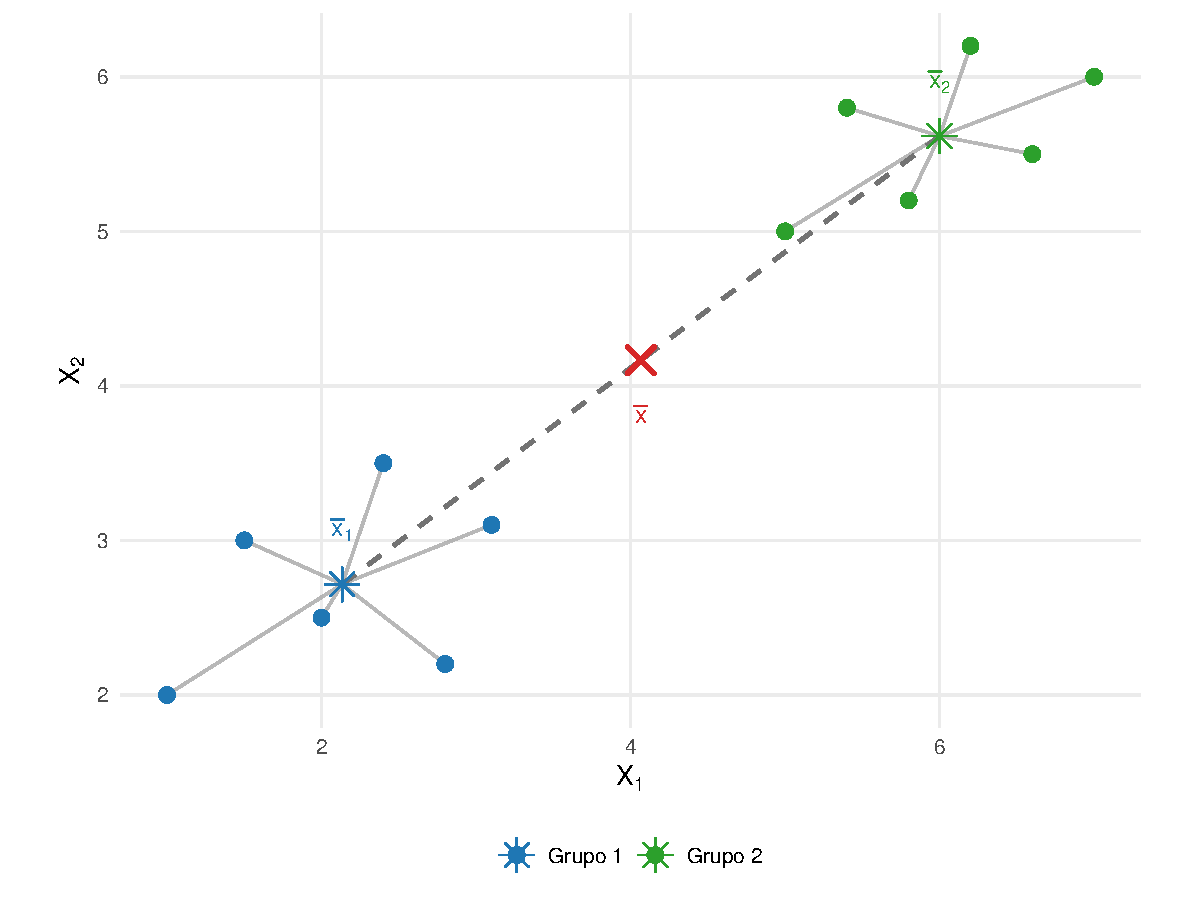
\includegraphics[keepaspectratio]{mod_2_covariancias_files/figure-pdf/fig-decomposicao-dispersao-grupos-1.pdf}}

}

\caption{\label{fig-decomposicao-dispersao-grupos}Decomposição
geométrica da dispersão em componentes intragrupos e entre grupos.}

\end{figure}%

\subsection{Dispersão total, intragrupos e entre
grupos}\label{dispersuxe3o-total-intragrupos-e-entre-grupos}

A matriz total é

\begin{equation}\phantomsection\label{eq-sscp-total-grupos}{
\mathbf T
=
\sum_{k=1}^K
\sum_{i=1}^{n_k}
\left(
\mathbf x_{ik}
-
\bar{\mathbf x}
\right)
\left(
\mathbf x_{ik}
-
\bar{\mathbf x}
\right)^\top.
}\end{equation}

\begin{definition}[Matriz de dispersão
intragrupos]\protect\hypertarget{def-sscp-intragrupos}{}\label{def-sscp-intragrupos}

A \textbf{matriz de dispersão intragrupos} é

\begin{equation}\phantomsection\label{eq-sscp-intragrupos}{
\mathbf T_{\mathrm{intra}}
=
\sum_{k=1}^K
\sum_{i=1}^{n_k}
\left(
\mathbf x_{ik}
-
\bar{\mathbf x}_k
\right)
\left(
\mathbf x_{ik}
-
\bar{\mathbf x}_k
\right)^\top
\in
\mathbb{R}^{p\times p}.
}\end{equation}

\end{definition}

Cada termo mede o afastamento de uma observação em relação ao centro de
seu próprio grupo.

\begin{definition}[Matriz de dispersão entre
grupos]\protect\hypertarget{def-sscp-entre-grupos}{}\label{def-sscp-entre-grupos}

A \textbf{matriz de dispersão entre grupos} é

\begin{equation}\phantomsection\label{eq-sscp-entre-grupos}{
\mathbf T_{\mathrm{entre}}
=
\sum_{k=1}^K
n_k
\left(
\bar{\mathbf x}_k
-
\bar{\mathbf x}
\right)
\left(
\bar{\mathbf x}_k
-
\bar{\mathbf x}
\right)^\top
\in
\mathbb{R}^{p\times p}.
}\end{equation}

\end{definition}

A ponderação por \(n_k\) registra o número de observações representadas
por cada média de grupo. Assim, um mesmo afastamento
\(\bar{\mathbf x}_k-\bar{\mathbf x}\) contribui mais para a dispersão
entre grupos quando corresponde a um grupo com maior número de
observações.

\begin{proposition}[Decomposição da dispersão
total]\protect\hypertarget{prp-decomposicao-dispersao-grupos}{}\label{prp-decomposicao-dispersao-grupos}

Para qualquer partição das \(n\) observações em \(K\) grupos não vazios,

\begin{equation}\phantomsection\label{eq-decomposicao-dispersao-grupos}{
\mathbf T
=
\mathbf T_{\mathrm{intra}}
+
\mathbf T_{\mathrm{entre}}.
}\end{equation}

\end{proposition}

\begin{proof}
Pela decomposição vetorial apresentada na
Equação~\ref{eq-decomposicao-vetor-desvio-grupos},

\[
\mathbf x_{ik}
-
\bar{\mathbf x}
=
\left(
\mathbf x_{ik}
-
\bar{\mathbf x}_k
\right)
+
\left(
\bar{\mathbf x}_k
-
\bar{\mathbf x}
\right).
\]

Ao formar o produto externo e somar sobre as observações, surgem duas
parcelas quadráticas e dois termos cruzados. Para cada grupo,

\[
\sum_{i=1}^{n_k}
\left(
\mathbf x_{ik}
-
\bar{\mathbf x}_k
\right)
=
\mathbf 0.
\]

Consequentemente, os termos cruzados desaparecem. A soma das primeiras
parcelas produz \(\mathbf T_{\mathrm{intra}}\), enquanto

\[
\sum_{i=1}^{n_k}
\left(
\bar{\mathbf x}_k
-
\bar{\mathbf x}
\right)
\left(
\bar{\mathbf x}_k
-
\bar{\mathbf x}
\right)^\top
=
n_k
\left(
\bar{\mathbf x}_k
-
\bar{\mathbf x}
\right)
\left(
\bar{\mathbf x}_k
-
\bar{\mathbf x}
\right)^\top.
\]

Somando sobre os grupos, obtém-se

\[
\mathbf T
=
\mathbf T_{\mathrm{intra}}
+
\mathbf T_{\mathrm{entre}}.
\]
\end{proof}

\begin{example}[Decomposição da dispersão em dois
grupos]\protect\hypertarget{exm-decomposicao-dispersao-grupos}{}\label{exm-decomposicao-dispersao-grupos}

Considere quatro observações de duas variáveis, distribuídas em dois
grupos:

\[
\begin{array}{c|cc}
\text{Grupo} & X_1 & X_2\\
\hline
1 & 1 & 1\\
1 & 3 & 1\\
2 & 3 & 5\\
2 & 5 & 5
\end{array}
\]

Assim,

\[
n_1=n_2=2,
\qquad
n=4,
\qquad
K=2.
\]

As médias dos grupos são

\[
\bar{\mathbf x}_1
=
\frac{1}{2}
\left[
\begin{bmatrix}
1\\
1
\end{bmatrix}
+
\begin{bmatrix}
3\\
1
\end{bmatrix}
\right]
=
\begin{bmatrix}
2\\
1
\end{bmatrix}
\]

e

\[
\bar{\mathbf x}_2
=
\frac{1}{2}
\left[
\begin{bmatrix}
3\\
5
\end{bmatrix}
+
\begin{bmatrix}
5\\
5
\end{bmatrix}
\right]
=
\begin{bmatrix}
4\\
5
\end{bmatrix}.
\]

A média total é

\[
\begin{aligned}
\bar{\mathbf x}
&=
\frac{1}{4}
\left[
\begin{bmatrix}
1\\
1
\end{bmatrix}
+
\begin{bmatrix}
3\\
1
\end{bmatrix}
+
\begin{bmatrix}
3\\
5
\end{bmatrix}
+
\begin{bmatrix}
5\\
5
\end{bmatrix}
\right]\\
&=
\begin{bmatrix}
3\\
3
\end{bmatrix}.
\end{aligned}
\]

Podemos agora calcular separadamente as três matrizes da decomposição.

\textbf{Dispersão intragrupos.}

No primeiro grupo,

\[
\mathbf x_{11}-\bar{\mathbf x}_1
=
\begin{bmatrix}
-1\\
0
\end{bmatrix}
\]

e

\[
\mathbf x_{21}-\bar{\mathbf x}_1
=
\begin{bmatrix}
1\\
0
\end{bmatrix}.
\]

Sua contribuição para a dispersão intragrupos é

\[
\begin{aligned}
\mathbf T_{\mathrm{intra},1}
&=
\begin{bmatrix}
-1\\
0
\end{bmatrix}
\begin{bmatrix}
-1 & 0
\end{bmatrix}
+
\begin{bmatrix}
1\\
0
\end{bmatrix}
\begin{bmatrix}
1 & 0
\end{bmatrix}\\
&=
\begin{bmatrix}
2 & 0\\
0 & 0
\end{bmatrix}.
\end{aligned}
\]

No segundo grupo,

\[
\mathbf x_{12}-\bar{\mathbf x}_2
=
\begin{bmatrix}
-1\\
0
\end{bmatrix}
\]

e

\[
\mathbf x_{22}-\bar{\mathbf x}_2
=
\begin{bmatrix}
1\\
0
\end{bmatrix},
\]

de modo que

\[
\mathbf T_{\mathrm{intra},2}
=
\begin{bmatrix}
2 & 0\\
0 & 0
\end{bmatrix}.
\]

Portanto,

\begin{equation}\phantomsection\label{eq-exemplo-dispersao-intragrupos}{
\begin{aligned}
\mathbf T_{\mathrm{intra}}
&=
\mathbf T_{\mathrm{intra},1}
+
\mathbf T_{\mathrm{intra},2}\\
&=
\begin{bmatrix}
4 & 0\\
0 & 0
\end{bmatrix}.
\end{aligned}
}\end{equation}

Toda a dispersão dentro dos grupos ocorre, neste exemplo, na primeira
variável. A segunda variável é constante dentro de cada grupo.

\textbf{Dispersão entre grupos.}

Os afastamentos das médias dos grupos em relação à média total são

\[
\bar{\mathbf x}_1-\bar{\mathbf x}
=
\begin{bmatrix}
-1\\
-2
\end{bmatrix}
\]

e

\[
\bar{\mathbf x}_2-\bar{\mathbf x}
=
\begin{bmatrix}
1\\
2
\end{bmatrix}.
\]

Como ambos os grupos possuem duas observações,

\begin{equation}\phantomsection\label{eq-exemplo-dispersao-entre-grupos}{
\begin{aligned}
\mathbf T_{\mathrm{entre}}
&=
2
\begin{bmatrix}
-1\\
-2
\end{bmatrix}
\begin{bmatrix}
-1 & -2
\end{bmatrix}
+
2
\begin{bmatrix}
1\\
2
\end{bmatrix}
\begin{bmatrix}
1 & 2
\end{bmatrix}\\
&=
2
\begin{bmatrix}
1 & 2\\
2 & 4
\end{bmatrix}
+
2
\begin{bmatrix}
1 & 2\\
2 & 4
\end{bmatrix}\\
&=
\begin{bmatrix}
4 & 8\\
8 & 16
\end{bmatrix}.
\end{aligned}
}\end{equation}

Nesse caso, a diferença entre os centros dos grupos envolve
simultaneamente as duas variáveis.

\textbf{Dispersão total.}

Calculando diretamente os desvios das quatro observações em relação a

\[
\bar{\mathbf x}
=
\begin{bmatrix}
3\\
3
\end{bmatrix},
\]

obtém-se

\begin{equation}\phantomsection\label{eq-exemplo-dispersao-total-grupos}{
\begin{aligned}
\mathbf T
&=
\begin{bmatrix}
-2\\
-2
\end{bmatrix}
\begin{bmatrix}
-2 & -2
\end{bmatrix}
+
\begin{bmatrix}
0\\
-2
\end{bmatrix}
\begin{bmatrix}
0 & -2
\end{bmatrix}\\
&\quad+
\begin{bmatrix}
0\\
2
\end{bmatrix}
\begin{bmatrix}
0 & 2
\end{bmatrix}
+
\begin{bmatrix}
2\\
2
\end{bmatrix}
\begin{bmatrix}
2 & 2
\end{bmatrix}\\
&=
\begin{bmatrix}
8 & 8\\
8 & 16
\end{bmatrix}.
\end{aligned}
}\end{equation}

A identidade Equação~\ref{eq-decomposicao-dispersao-grupos} pode então
ser verificada diretamente:

\[
\begin{aligned}
\mathbf T_{\mathrm{intra}}
+
\mathbf T_{\mathrm{entre}}
&=
\begin{bmatrix}
4 & 0\\
0 & 0
\end{bmatrix}
+
\begin{bmatrix}
4 & 8\\
8 & 16
\end{bmatrix}\\
&=
\begin{bmatrix}
8 & 8\\
8 & 16
\end{bmatrix}\\
&=
\mathbf T.
\end{aligned}
\]

A decomposição também pode ser examinada em direções específicas. Para

\[
\mathbf a_1
=
\begin{bmatrix}
1\\
0
\end{bmatrix},
\]

que seleciona a primeira variável,

\[
\mathbf a_1^\top
\mathbf T
\mathbf a_1
=
8,
\]

com

\[
\mathbf a_1^\top
\mathbf T_{\mathrm{intra}}
\mathbf a_1
=
4
\]

e

\[
\mathbf a_1^\top
\mathbf T_{\mathrm{entre}}
\mathbf a_1
=
4.
\]

Assim,

\[
8=4+4.
\]

Metade da dispersão de \(X_1\) decorre de diferenças dentro dos grupos e
metade das diferenças entre seus centros.

Para

\[
\mathbf a_2
=
\begin{bmatrix}
0\\
1
\end{bmatrix},
\]

que seleciona a segunda variável,

\[
\mathbf a_2^\top
\mathbf T
\mathbf a_2
=
16,
\]

enquanto

\[
\mathbf a_2^\top
\mathbf T_{\mathrm{intra}}
\mathbf a_2
=
0
\]

e

\[
\mathbf a_2^\top
\mathbf T_{\mathrm{entre}}
\mathbf a_2
=
16.
\]

Portanto,

\[
16=0+16.
\]

A variável \(X_2\) não apresenta dispersão dentro dos grupos neste
conjunto de dados; toda a sua dispersão total está associada à diferença
entre as médias dos dois grupos.

O exemplo mostra que a identidade

\[
\mathbf T
=
\mathbf T_{\mathrm{intra}}
+
\mathbf T_{\mathrm{entre}}
\]

expressa simultaneamente a decomposição da dispersão em todas as
direções. Para qualquer combinação linear das variáveis, a dispersão
total dessa combinação também se decompõe nas parcelas intragrupos e
entre grupos, conforme Equação~\ref{eq-decomposicao-dispersao-direcao}.

\end{example}

A identidade Equação~\ref{eq-decomposicao-dispersao-grupos} é algébrica
e depende somente da partição das observações e das definições das
médias total e de grupo (Rencher; Christensen, 2012). Normalidade,
independência e outros pressupostos probabilísticos não são necessários
para estabelecê-la.

Para qualquer direção

\[
\mathbf a
\in
\mathbb{R}^p,
\]

tem-se

\begin{equation}\phantomsection\label{eq-decomposicao-dispersao-direcao}{
\mathbf a^\top
\mathbf T
\mathbf a
=
\mathbf a^\top
\mathbf T_{\mathrm{intra}}
\mathbf a
+
\mathbf a^\top
\mathbf T_{\mathrm{entre}}
\mathbf a.
}\end{equation}

Se

\[
y_{ik}
=
\mathbf a^\top
\mathbf x_{ik},
\]

então Equação~\ref{eq-decomposicao-dispersao-direcao} corresponde
exatamente à decomposição univariada

\begin{equation}\phantomsection\label{eq-decomposicao-dispersao-univariada}{
\sum_{k=1}^K
\sum_{i=1}^{n_k}
\left(
y_{ik}
-
\bar{y}
\right)^2
=
\sum_{k=1}^K
\sum_{i=1}^{n_k}
\left(
y_{ik}
-
\bar{y}_k
\right)^2
+
\sum_{k=1}^K
n_k
\left(
\bar{y}_k
-
\bar{y}
\right)^2.
}\end{equation}

A decomposição matricial reúne simultaneamente essa identidade para
todas as combinações lineares das variáveis.

\subsection{Somas de quadrados e traço das matrizes de
dispersão}\label{somas-de-quadrados-e-trauxe7o-das-matrizes-de-dispersuxe3o}

As matrizes \(\mathbf T\), \(\mathbf T_{\mathrm{intra}}\) e
\(\mathbf T_{\mathrm{entre}}\) são matrizes de somas de quadrados e
produtos cruzados e descrevem simultaneamente a dispersão das diferentes
variáveis e suas associações.

O traço dessas matrizes reúne apenas os termos quadráticos da diagonal e
fornece uma medida escalar de dispersão. Defina

\[
SQ_{\mathrm{total}}
=
\operatorname{tr}
\left(
\mathbf T
\right),
\]

\[
SQ_{\mathrm{intra}}
=
\operatorname{tr}
\left(
\mathbf T_{\mathrm{intra}}
\right)
\]

e

\[
SQ_{\mathrm{entre}}
=
\operatorname{tr}
\left(
\mathbf T_{\mathrm{entre}}
\right).
\]

Essas quantidades constituem as somas de quadrados total, intragrupos e
entre grupos, respectivamente. No caso univariado, elas coincidem com as
somas de quadrados usuais da análise de variância. No caso multivariado,
correspondem à soma das somas de quadrados das \(p\) variáveis.

Como o traço soma as contribuições das diferentes variáveis, essas
quantidades dependem das escalas em que as variáveis são expressas. Sua
interpretação conjunta é mais direta quando as variáveis possuem
unidades comparáveis ou quando uma padronização apropriada foi
realizada.

Para a matriz de dispersão total,

\[
\mathbf T
=
\sum_{k=1}^K
\sum_{i=1}^{n_k}
\left(
\mathbf x_{ik}
-
\bar{\mathbf x}
\right)
\left(
\mathbf x_{ik}
-
\bar{\mathbf x}
\right)^\top,
\]

tem-se

\begin{equation}\phantomsection\label{eq-traco-dispersao-total-grupos}{
\begin{aligned}
\operatorname{tr}
\left(
\mathbf T
\right)
&=
\sum_{k=1}^K
\sum_{i=1}^{n_k}
\operatorname{tr}
\left[
\left(
\mathbf x_{ik}
-
\bar{\mathbf x}
\right)
\left(
\mathbf x_{ik}
-
\bar{\mathbf x}
\right)^\top
\right]\\
&=
\sum_{k=1}^K
\sum_{i=1}^{n_k}
\left\|
\mathbf x_{ik}
-
\bar{\mathbf x}
\right\|^2.
\end{aligned}
}\end{equation}

Portanto,

\begin{equation}\phantomsection\label{eq-sq-total-grupos}{
SQ_{\mathrm{total}}
=
\operatorname{tr}
\left(
\mathbf T
\right)
=
\sum_{k=1}^K
\sum_{i=1}^{n_k}
\left\|
\mathbf x_{ik}
-
\bar{\mathbf x}
\right\|^2.
}\end{equation}

Assim, \(SQ_{\mathrm{total}}\) é a soma dos quadrados das distâncias
euclidianas das observações à média total.

Analogamente,

\begin{equation}\phantomsection\label{eq-sq-intragrupos}{
SQ_{\mathrm{intra}}
=
\operatorname{tr}
\left(
\mathbf T_{\mathrm{intra}}
\right)
=
\sum_{k=1}^K
\sum_{i=1}^{n_k}
\left\|
\mathbf x_{ik}
-
\bar{\mathbf x}_k
\right\|^2
}\end{equation}

mede a soma dos quadrados dos afastamentos das observações em relação
aos centros de seus respectivos grupos.

Por sua vez,

\begin{equation}\phantomsection\label{eq-sq-entre-grupos}{
SQ_{\mathrm{entre}}
=
\operatorname{tr}
\left(
\mathbf T_{\mathrm{entre}}
\right)
=
\sum_{k=1}^K
n_k
\left\|
\bar{\mathbf x}_k
-
\bar{\mathbf x}
\right\|^2
}\end{equation}

mede a soma ponderada dos quadrados das distâncias entre os centros dos
grupos e a média total.

Como

\[
\mathbf T
=
\mathbf T_{\mathrm{intra}}
+
\mathbf T_{\mathrm{entre}},
\]

a linearidade do traço fornece

\begin{equation}\phantomsection\label{eq-decomposicao-somas-quadrados-grupos}{
SQ_{\mathrm{total}}
=
SQ_{\mathrm{intra}}
+
SQ_{\mathrm{entre}}.
}\end{equation}

Equivalentemente,

\begin{equation}\phantomsection\label{eq-decomposicao-traco-dispersao-grupos}{
\operatorname{tr}
\left(
\mathbf T
\right)
=
\operatorname{tr}
\left(
\mathbf T_{\mathrm{intra}}
\right)
+
\operatorname{tr}
\left(
\mathbf T_{\mathrm{entre}}
\right).
}\end{equation}

Ao tomar o traço da decomposição matricial, recupera-se uma identidade
escalar análoga à decomposição de somas de quadrados familiar da análise
de variância:

\[
SQ_{\mathrm{total}}
=
SQ_{\mathrm{intra}}
+
SQ_{\mathrm{entre}}.
\]

A decomposição matricial

\[
\mathbf T
=
\mathbf T_{\mathrm{intra}}
+
\mathbf T_{\mathrm{entre}}
\]

é mais informativa, pois preserva também os produtos cruzados entre as
variáveis. O traço resume essa estrutura matricial em uma única soma de
quadrados.

Assim, a decomposição matricial da dispersão também produz uma
decomposição da quantidade total de dispersão medida pelas distâncias
euclidianas quadráticas.

Dividindo essas somas por \(n\), obtêm-se medidas médias da dispersão
quadrática. Por exemplo,

\[
\frac{SQ_{\mathrm{total}}}{n}
=
\frac{1}{n}
\operatorname{tr}
\left(
\mathbf T
\right)
=
\frac{1}{n}
\sum_{k=1}^K
\sum_{i=1}^{n_k}
\left\|
\mathbf x_{ik}
-
\bar{\mathbf x}
\right\|^2.
\]

Essa quantidade representa o afastamento quadrático médio das
observações em relação à média total. De modo correspondente,

\[
\frac{SQ_{\mathrm{intra}}}{n}
\]

e

\[
\frac{SQ_{\mathrm{entre}}}{n}
\]

representam, respectivamente, as contribuições médias da dispersão
intragrupos e entre grupos.

\subsection{Esperança das matrizes de dispersão por
grupos}\label{esperanuxe7a-das-matrizes-de-dispersuxe3o-por-grupos}

Até este ponto, a decomposição

\[
\mathbf T
=
\mathbf T_{\mathrm{intra}}
+
\mathbf T_{\mathrm{entre}}
\]

foi tratada como uma identidade algébrica para os dados observados. É
possível também examinar essas matrizes como objetos aleatórios e
calcular suas esperanças, desde que se especifique uma estrutura
probabilística para as observações.

Suponha que, para cada grupo \(k=1,\ldots,K\),

\[
\boldsymbol{\mathsf X}_{ik},
\qquad
i=1,\ldots,n_k,
\]

sejam vetores aleatórios independentes, com

\[
E
\left(
\boldsymbol{\mathsf X}_{ik}
\right)
=
\boldsymbol{\mu}_k
\]

e matriz de covariâncias comum

\[
\operatorname{Cov}
\left(
\boldsymbol{\mathsf X}_{ik}
\right)
=
\boldsymbol{\Sigma}.
\]

Não é necessário assumir normalidade.

Defina a média populacional ponderada dos grupos por

\begin{equation}\phantomsection\label{eq-media-populacional-ponderada-grupos}{
\boldsymbol{\mu}
=
\frac{1}{n}
\sum_{k=1}^K
n_k
\boldsymbol{\mu}_k.
}\end{equation}

Considere ainda a matriz

\begin{equation}\phantomsection\label{eq-dispersao-populacional-entre-medias}{
\mathbf B_{\mu}
=
\sum_{k=1}^K
n_k
\left(
\boldsymbol{\mu}_k
-
\boldsymbol{\mu}
\right)
\left(
\boldsymbol{\mu}_k
-
\boldsymbol{\mu}
\right)^\top,
}\end{equation}

que representa a dispersão entre os vetores de médias populacionais dos
grupos.

Quando as matrizes de dispersão são consideradas objetos aleatórios, as
somas de quadrados correspondentes também são objetos aleatórios. Defina

\[
\mathsf{SQ}_{\mathrm{total}}
=
\operatorname{tr}
\left(
\boldsymbol{\mathsf T}
\right),
\]

\[
\mathsf{SQ}_{\mathrm{intra}}
=
\operatorname{tr}
\left(
\boldsymbol{\mathsf T}_{\mathrm{intra}}
\right)
\]

e

\[
\mathsf{SQ}_{\mathrm{entre}}
=
\operatorname{tr}
\left(
\boldsymbol{\mathsf T}_{\mathrm{entre}}
\right).
\]

Suas realizações observadas são, respectivamente,

\[
SQ_{\mathrm{total}},
\qquad
SQ_{\mathrm{intra}}
\qquad
\text{e}
\qquad
SQ_{\mathrm{entre}}.
\]

Para a matriz de dispersão intragrupos,

\[
\boldsymbol{\mathsf T}_{\mathrm{intra}}
=
\sum_{k=1}^K
\sum_{i=1}^{n_k}
\left(
\boldsymbol{\mathsf X}_{ik}
-
\bar{\boldsymbol{\mathsf X}}_k
\right)
\left(
\boldsymbol{\mathsf X}_{ik}
-
\bar{\boldsymbol{\mathsf X}}_k
\right)^\top,
\]

tem-se

\begin{equation}\phantomsection\label{eq-esperanca-dispersao-intragrupos}{
E
\left(
\boldsymbol{\mathsf T}_{\mathrm{intra}}
\right)
=
(n-K)
\boldsymbol{\Sigma}.
}\end{equation}

Tomando o traço dos dois lados e utilizando a linearidade do traço e da
esperança,

\[
E
\left(
\mathsf{SQ}_{\mathrm{intra}}
\right)
=
(n-K)
\operatorname{tr}
\left(
\boldsymbol{\Sigma}
\right).
\]

Consequentemente,

\[
E
\left(
\frac{
\mathsf{SQ}_{\mathrm{intra}}
}{
n-K
}
\right)
=
\operatorname{tr}
\left(
\boldsymbol{\Sigma}
\right).
\]

Dentro de cada grupo, os vetores centralizados satisfazem

\[
\sum_{i=1}^{n_k}
\left(
\boldsymbol{\mathsf X}_{ik}
-
\bar{\boldsymbol{\mathsf X}}_k
\right)
=
\mathbf 0.
\]

Assim, a centralização pela média do grupo reduz em uma unidade a
dimensão disponível, fazendo com que o grupo \(k\) contribua com
\(n_k-1\) graus de liberdade. Portanto,

\[
\sum_{k=1}^K
(n_k-1)
=
n-K.
\]

A quantidade \(n-K\) corresponde, assim, aos graus de liberdade
intragrupos familiares da análise de variância. A divisão por \(n-K\)
antecipa a construção dos quadrados médios utilizada em ANOVA e
planejamento de experimentos.

Para a dispersão entre grupos,

\[
\boldsymbol{\mathsf T}_{\mathrm{entre}}
=
\sum_{k=1}^K
n_k
\left(
\bar{\boldsymbol{\mathsf X}}_k
-
\bar{\boldsymbol{\mathsf X}}
\right)
\left(
\bar{\boldsymbol{\mathsf X}}_k
-
\bar{\boldsymbol{\mathsf X}}
\right)^\top,
\]

a esperança é

\begin{equation}\phantomsection\label{eq-esperanca-dispersao-entre-grupos}{
E
\left(
\boldsymbol{\mathsf T}_{\mathrm{entre}}
\right)
=
(K-1)
\boldsymbol{\Sigma}
+
\mathbf B_{\mu}.
}\end{equation}

Essa expressão contém duas parcelas com interpretações distintas. O
termo

\[
(K-1)
\boldsymbol{\Sigma}
\]

representa a variabilidade decorrente do fato de que as médias amostrais
dos grupos variam de amostra para amostra, enquanto

\[
\mathbf B_{\mu}
\]

representa a separação efetiva entre os vetores de médias populacionais.

Em particular, se

\[
\boldsymbol{\mu}_1
=
\cdots
=
\boldsymbol{\mu}_K,
\]

então

\[
\mathbf B_{\mu}
=
\mathbf 0,
\]

mas, ainda assim,

\[
E
\left(
\boldsymbol{\mathsf T}_{\mathrm{entre}}
\right)
=
(K-1)
\boldsymbol{\Sigma}.
\]

Tomando o traço na Equação~\ref{eq-esperanca-dispersao-entre-grupos},

\[
E
\left(
\mathsf{SQ}_{\mathrm{entre}}
\right)
=
(K-1)
\operatorname{tr}
\left(
\boldsymbol{\Sigma}
\right)
+
\operatorname{tr}
\left(
\mathbf B_{\mu}
\right).
\]

Consequentemente,

\[
E
\left(
\frac{
\mathsf{SQ}_{\mathrm{entre}}
}{
K-1
}
\right)
=
\operatorname{tr}
\left(
\boldsymbol{\Sigma}
\right)
+
\frac{
\operatorname{tr}
\left(
\mathbf B_{\mu}
\right)
}{
K-1
}.
\]

Quando os grupos possuem o mesmo vetor de médias populacional,

\[
\boldsymbol{\mu}_1
=
\cdots
=
\boldsymbol{\mu}_K,
\]

tem-se

\[
\mathbf B_{\mu}
=
\mathbf 0.
\]

Nesse caso,

\[
E
\left(
\frac{
\mathsf{SQ}_{\mathrm{entre}}
}{
K-1
}
\right)
=
E
\left(
\frac{
\mathsf{SQ}_{\mathrm{intra}}
}{
n-K
}
\right)
=
\operatorname{tr}
\left(
\boldsymbol{\Sigma}
\right).
\]

Portanto, quando não existe separação entre os vetores de médias
populacionais, as somas de quadrados intragrupos e entre grupos, após a
divisão pelas respectivas quantidades \(n-K\) e \(K-1\), possuem a mesma
esperança.

Isso ocorre porque as médias amostrais dos grupos não coincidem
exatamente, mesmo quando seus vetores de médias populacionais são
iguais.

Por fim, como

\[
\boldsymbol{\mathsf T}
=
\boldsymbol{\mathsf T}_{\mathrm{intra}}
+
\boldsymbol{\mathsf T}_{\mathrm{entre}},
\]

a linearidade da esperança fornece

\begin{equation}\phantomsection\label{eq-esperanca-dispersao-total-grupos}{
\begin{aligned}
E
\left(
\boldsymbol{\mathsf T}
\right)
&=
E
\left(
\boldsymbol{\mathsf T}_{\mathrm{intra}}
\right)
+
E
\left(
\boldsymbol{\mathsf T}_{\mathrm{entre}}
\right)\\
&=
(n-1)
\boldsymbol{\Sigma}
+
\mathbf B_{\mu}.
\end{aligned}
}\end{equation} Tomando o traço,

\begin{equation}\phantomsection\label{eq-esperanca-sq-total-grupos}{
E
\left(
\mathsf{SQ}_{\mathrm{total}}
\right)
=
(n-1)
\operatorname{tr}
\left(
\boldsymbol{\Sigma}
\right)
+
\operatorname{tr}
\left(
\mathbf B_{\mu}
\right).
}\end{equation}

Além disso,

\[
\mathsf{SQ}_{\mathrm{total}}
=
\mathsf{SQ}_{\mathrm{intra}}
+
\mathsf{SQ}_{\mathrm{entre}},
\]

que é a versão aleatória da decomposição observada

\[
SQ_{\mathrm{total}}
=
SQ_{\mathrm{intra}}
+
SQ_{\mathrm{entre}}.
\]

Quando todos os grupos possuem o mesmo vetor de médias populacional,

\[
E
\left(
\boldsymbol{\mathsf T}
\right)
=
(n-1)
\boldsymbol{\Sigma}.
\]

Esses resultados dependem apenas de momentos de primeira e segunda ordem
e da independência entre as observações; a normalidade não é necessária.
Distribuições amostrais e resultados inferenciais associados a essas
matrizes serão tratados posteriormente.

No caso univariado, as matrizes reduzem-se a escalares e a decomposição
assume a forma familiar

\[
SQ_{\mathrm{total}}
=
SQ_{\mathrm{intra}}
+
SQ_{\mathrm{entre}}.
\]

As divisões

\[
QM_{\mathrm{intra}}
=
\frac{
SQ_{\mathrm{intra}}
}{
n-K
}
\]

e

\[
QM_{\mathrm{entre}}
=
\frac{
SQ_{\mathrm{entre}}
}{
K-1
}
\]

correspondem aos quadrados médios familiares da análise de variância e
do planejamento de experimentos.

No contexto multivariado, contudo, as matrizes completas de somas de
quadrados e produtos cruzados preservam informações adicionais sobre as
associações entre as variáveis. Por essa razão, métodos multivariados
posteriores utilizarão \(\mathbf T_{\mathrm{intra}}\) e
\(\mathbf T_{\mathrm{entre}}\), e não apenas seus traços.

\subsection{Propriedades e limites de
posto}\label{propriedades-e-limites-de-posto}

Independentemente das hipóteses probabilísticas utilizadas na subseção
anterior, as propriedades estruturais a seguir decorrem diretamente das
definições das matrizes de dispersão.

\begin{proposition}[Estrutura das matrizes de dispersão por
grupos]\protect\hypertarget{prp-estrutura-decomposicao-dispersao-grupos}{}\label{prp-estrutura-decomposicao-dispersao-grupos}

As matrizes

\[
\mathbf T,
\qquad
\mathbf T_{\mathrm{intra}}
\qquad
\text{e}
\qquad
\mathbf T_{\mathrm{entre}}
\]

são simétricas e positivas semidefinidas. Além disso,

\[
\mathbf 0
\preceq
\mathbf T_{\mathrm{intra}}
\preceq
\mathbf T
\]

e

\[
\mathbf 0
\preceq
\mathbf T_{\mathrm{entre}}
\preceq
\mathbf T.
\]

Seus postos satisfazem

\[
\operatorname{posto}
\left(
\mathbf T
\right)
\leq
\min(p,n-1),
\]

\begin{equation}\phantomsection\label{eq-posto-sscp-intragrupos}{
\operatorname{posto}
\left(
\mathbf T_{\mathrm{intra}}
\right)
\leq
\min(p,n-K),
}\end{equation}

e

\begin{equation}\phantomsection\label{eq-posto-sscp-entre-grupos}{
\operatorname{posto}
\left(
\mathbf T_{\mathrm{entre}}
\right)
\leq
\min(p,K-1).
}\end{equation}

\end{proposition}

\begin{proof}
Para qualquer \(\mathbf a\in\mathbb{R}^p\),

\[
\mathbf a^\top
\mathbf T_{\mathrm{intra}}
\mathbf a
=
\sum_{k=1}^K
\sum_{i=1}^{n_k}
\left[
\mathbf a^\top
\left(
\mathbf x_{ik}
-
\bar{\mathbf x}_k
\right)
\right]^2
\geq
0
\]

e

\[
\mathbf a^\top
\mathbf T_{\mathrm{entre}}
\mathbf a
=
\sum_{k=1}^K
n_k
\left[
\mathbf a^\top
\left(
\bar{\mathbf x}_k
-
\bar{\mathbf x}
\right)
\right]^2
\geq
0.
\]

Logo, as duas parcelas são positivas semidefinidas. Pela identidade
Equação~\ref{eq-decomposicao-dispersao-grupos},

\[
\mathbf T
-
\mathbf T_{\mathrm{intra}}
=
\mathbf T_{\mathrm{entre}}
\succeq
\mathbf 0
\]

e

\[
\mathbf T
-
\mathbf T_{\mathrm{entre}}
=
\mathbf T_{\mathrm{intra}}
\succeq
\mathbf 0,
\]

o que estabelece as relações na ordem de Loewner.

O limite para \(\mathbf T\) foi obtido na
Equação~\ref{eq-posto-sscp-total}.

Dentro do grupo \(k\), os \(n_k\) vetores centralizados satisfazem

\[
\sum_{i=1}^{n_k}
\left(
\mathbf x_{ik}
-
\bar{\mathbf x}_k
\right)
=
\mathbf 0.
\]

Assim, os vetores centralizados desse grupo geram um subespaço de
dimensão no máximo \(n_k-1\). Considerando todos os grupos,

\[
\sum_{k=1}^K
(n_k-1)
=
n-K,
\]

e, portanto,

\[
\operatorname{posto}
\left(
\mathbf T_{\mathrm{intra}}
\right)
\leq
\min(p,n-K).
\]

Para a parcela entre grupos,

\[
\sum_{k=1}^K
n_k
\left(
\bar{\mathbf x}_k
-
\bar{\mathbf x}
\right)
=
\mathbf 0.
\]

Os \(K\) vetores

\[
\sqrt{n_k}
\left(
\bar{\mathbf x}_k
-
\bar{\mathbf x}
\right)
\]

geram, portanto, um subespaço de dimensão no máximo \(K-1\).
Consequentemente,

\[
\operatorname{posto}
\left(
\mathbf T_{\mathrm{entre}}
\right)
\leq
\min(p,K-1).
\]
\end{proof}

Os limites podem ser estritos quando existem relações lineares
adicionais entre as variáveis ou entre os vetores de médias dos grupos.

As relações na ordem de Loewner implicam, para qualquer direção
\(\mathbf a\),

\[
0
\leq
\mathbf a^\top
\mathbf T_{\mathrm{intra}}
\mathbf a
\leq
\mathbf a^\top
\mathbf T
\mathbf a
\]

e

\[
0
\leq
\mathbf a^\top
\mathbf T_{\mathrm{entre}}
\mathbf a
\leq
\mathbf a^\top
\mathbf T
\mathbf a.
\]

Assim, a dispersão intragrupos ou entre grupos em uma direção não pode
exceder a dispersão total na mesma direção.

Dois casos extremos auxiliam a interpretação. Se

\[
\bar{\mathbf x}_1
=
\cdots
=
\bar{\mathbf x}_K
=
\bar{\mathbf x},
\]

então

\[
\mathbf T_{\mathrm{entre}}
=
\mathbf 0.
\]

Se, por outro lado, todas as observações de cada grupo coincidem com a
respectiva média,

\[
\mathbf x_{ik}
=
\bar{\mathbf x}_k,
\]

então

\[
\mathbf T_{\mathrm{intra}}
=
\mathbf 0.
\]

Neste capítulo, a identidade

\[
\mathbf T
=
\mathbf T_{\mathrm{intra}}
+
\mathbf T_{\mathrm{entre}}
\]

é inicialmente desenvolvida como uma decomposição algébrica da dispersão
observada e, sob hipóteses explícitas de independência e covariância
comum, recebe também uma interpretação por meio das esperanças das
matrizes de dispersão. Distribuições amostrais, testes de hipóteses e
sua formulação no modelo linear multivariado serão desenvolvidos
posteriormente.

No Capítulo 11, uma estrutura correspondente será obtida a partir do
modelo linear multivariado e de matrizes de projeção. Graus de
liberdade, estimadores de covariâncias residuais e hipóteses lineares
pertencem àquele contexto.

\section{Síntese do capítulo}\label{suxedntese-do-capuxedtulo-7}

A matriz de covariâncias

\[
\boldsymbol{\Sigma}
=
\operatorname{Cov}
\left(
\boldsymbol{\mathsf X}
\right)
\]

representa a estrutura de segunda ordem de um vetor aleatório. Sua
diagonal contém as variâncias das componentes, e seus elementos fora da
diagonal registram covariâncias. Para qualquer combinação linear,

\[
\operatorname{Var}
\left(
\mathbf a^\top
\boldsymbol{\mathsf X}
\right)
=
\mathbf a^\top
\boldsymbol{\Sigma}
\mathbf a,
\]

de modo que a matriz de covariâncias determina a dispersão em todas as
direções.

A padronização marginal conduz à matriz de correlações

\[
\boldsymbol{\mathcal R}
=
\mathbf D_{\Sigma}^{-1/2}
\boldsymbol{\Sigma}
\mathbf D_{\Sigma}^{-1/2},
\]

que preserva a estrutura de associação linear após a retirada das
escalas marginais.

A decomposição espectral de \(\boldsymbol{\Sigma}\) fornece eixos
ortogonais de dispersão, enquanto o traço e o determinante produzem
resumos escalares distintos. A variância total é

\[
\operatorname{tr}
\left(
\boldsymbol{\Sigma}
\right)
=
\sum_{j=1}^p
\sigma_{jj}
=
\sum_{j=1}^p
\lambda_j,
\]

e também pode ser interpretada como o afastamento euclidiano quadrático
médio do vetor aleatório em relação ao seu centro:

\[
E
\left[
\left\|
\boldsymbol{\mathsf X}
-
\boldsymbol{\mu}
\right\|^2
\right]
=
\operatorname{tr}
\left(
\boldsymbol{\Sigma}
\right).
\]

Mais geralmente, para uma matriz simétrica \(\mathbf A\) e um vetor fixo
\(\mathbf a\),

\[
E
\left[
\left(
\boldsymbol{\mathsf X}
-
\mathbf a
\right)^\top
\mathbf A
\left(
\boldsymbol{\mathsf X}
-
\mathbf a
\right)
\right]
=
\operatorname{tr}
\left(
\mathbf A
\boldsymbol{\Sigma}
\right)
+
\left(
\boldsymbol{\mu}
-
\mathbf a
\right)^\top
\mathbf A
\left(
\boldsymbol{\mu}
-
\mathbf a
\right).
\]

A variância generalizada é

\[
\det
\left(
\boldsymbol{\Sigma}
\right),
\]

e, quando \(\boldsymbol{\Sigma}\succ\mathbf 0\), a distância de
Mahalanobis

\[
d_M^2
\left(
\mathbf x,
\boldsymbol{\mu}
\right)
=
\left(
\mathbf x-\boldsymbol{\mu}
\right)^\top
\boldsymbol{\Sigma}^{-1}
\left(
\mathbf x-\boldsymbol{\mu}
\right)
\]

mede afastamentos levando em conta simultaneamente escalas e
covariâncias. Sua esperança populacional satisfaz

\[
E
\left[
d_M^2
\left(
\boldsymbol{\mathsf X},
\boldsymbol{\mu}
\right)
\right]
=
p.
\]

A transformação de \textbf{branqueamento} (\emph{whitening}), também
denominada \textbf{esferização}, transforma a estrutura de covariâncias
em identidade. No branqueamento simétrico,

\[
\boldsymbol{\mathsf Z}
=
\boldsymbol{\Sigma}^{-1/2}
\left(
\boldsymbol{\mathsf X}
-
\boldsymbol{\mu}
\right),
\]

e

\[
\operatorname{Cov}
\left(
\boldsymbol{\mathsf Z}
\right)
=
\mathbf I_p.
\]

Nesse espaço transformado, a distância de Mahalanobis coincide com a
distância euclidiana. A padronização marginal e o branqueamento diferem
porque a primeira produz matriz de covariâncias igual a
\(\boldsymbol{\mathcal R}\), enquanto o branqueamento produz
\(\mathbf I_p\).

No nível descritivo, as mesmas estruturas são representadas por

\[
\mathbf T
=
\mathbf X_c^\top
\mathbf X_c,
\qquad
\mathbf S
=
\frac{1}{n-1}
\mathbf T
\]

e

\[
\mathbf R
=
\mathbf D_S^{-1/2}
\mathbf S
\mathbf D_S^{-1/2}.
\]

A sigla \textbf{SQPC} significa \textbf{somas de quadrados e produtos
cruzados} e será utilizada como equivalente, em português, à sigla
inglesa \textbf{SSCP}, de \emph{sum of squares and cross-products}.

Quando as observações estão organizadas em grupos,

\[
\mathbf T
=
\mathbf T_{\mathrm{intra}}
+
\mathbf T_{\mathrm{entre}}
\]

separa a dispersão observada dentro dos grupos da dispersão associada às
diferenças entre seus centros. As matrizes completas preservam tanto as
somas de quadrados de cada variável quanto os produtos cruzados entre
variáveis.

Tomando o traço, obtém-se a decomposição escalar

\[
SQ_{\mathrm{total}}
=
SQ_{\mathrm{intra}}
+
SQ_{\mathrm{entre}},
\]

em que

\[
SQ_{\mathrm{total}}
=
\operatorname{tr}
\left(
\mathbf T
\right),
\qquad
SQ_{\mathrm{intra}}
=
\operatorname{tr}
\left(
\mathbf T_{\mathrm{intra}}
\right)
\]

e

\[
SQ_{\mathrm{entre}}
=
\operatorname{tr}
\left(
\mathbf T_{\mathrm{entre}}
\right).
\]

No caso univariado, essa identidade coincide com a decomposição de somas
de quadrados familiar da análise de variância. Os correspondentes
quadrados médios são

\[
QM_{\mathrm{intra}}
=
\frac{
SQ_{\mathrm{intra}}
}{
n-K
}
\]

e

\[
QM_{\mathrm{entre}}
=
\frac{
SQ_{\mathrm{entre}}
}{
K-1
}.
\]

No contexto multivariado, entretanto, as matrizes
\(\mathbf T_{\mathrm{intra}}\) e \(\mathbf T_{\mathrm{entre}}\) contêm
informação adicional sobre os produtos cruzados e, por isso, são mais
informativas do que seus traços.

Sob independência entre as observações e matriz de covariâncias comum
\(\boldsymbol{\Sigma}\) nos grupos, as matrizes de dispersão também
admitem interpretações probabilísticas. Se

\[
\boldsymbol{\mu}
=
\frac{1}{n}
\sum_{k=1}^K
n_k
\boldsymbol{\mu}_k
\]

e

\[
\mathbf B_{\mu}
=
\sum_{k=1}^K
n_k
\left(
\boldsymbol{\mu}_k
-
\boldsymbol{\mu}
\right)
\left(
\boldsymbol{\mu}_k
-
\boldsymbol{\mu}
\right)^\top,
\]

então

\[
E
\left(
\boldsymbol{\mathsf T}_{\mathrm{intra}}
\right)
=
(n-K)
\boldsymbol{\Sigma},
\]

\[
E
\left(
\boldsymbol{\mathsf T}_{\mathrm{entre}}
\right)
=
(K-1)
\boldsymbol{\Sigma}
+
\mathbf B_{\mu},
\]

e

\[
E
\left(
\boldsymbol{\mathsf T}
\right)
=
(n-1)
\boldsymbol{\Sigma}
+
\mathbf B_{\mu}.
\] Tomando os traços,

\[
E
\left(
\mathsf{SQ}_{\mathrm{intra}}
\right)
=
(n-K)
\operatorname{tr}
\left(
\boldsymbol{\Sigma}
\right)
\]

e

\[
E
\left(
\mathsf{SQ}_{\mathrm{entre}}
\right)
=
(K-1)
\operatorname{tr}
\left(
\boldsymbol{\Sigma}
\right)
+
\operatorname{tr}
\left(
\mathbf B_{\mu}
\right).
\]

Definindo os quadrados médios como objetos aleatórios por

\[
\mathsf{QM}_{\mathrm{intra}}
=
\frac{
\mathsf{SQ}_{\mathrm{intra}}
}{
n-K
}
\]

e

\[
\mathsf{QM}_{\mathrm{entre}}
=
\frac{
\mathsf{SQ}_{\mathrm{entre}}
}{
K-1
},
\]

quando

\[
\boldsymbol{\mu}_1
=
\cdots
=
\boldsymbol{\mu}_K,
\]

tem-se

\[
E
\left(
\mathsf{QM}_{\mathrm{intra}}
\right)
=
E
\left(
\mathsf{QM}_{\mathrm{entre}}
\right)
=
\operatorname{tr}
\left(
\boldsymbol{\Sigma}
\right).
\]

Essa igualdade antecipa a lógica dos quadrados médios da análise de
variância, enquanto a formulação multivariada posterior utilizará as
matrizes completas de somas de quadrados e produtos cruzados.

A Tabela~\ref{tbl-sintese-covariancias} reúne os principais objetos do
capítulo.

\begin{longtable}[]{@{}
  >{\raggedright\arraybackslash}p{(\linewidth - 6\tabcolsep) * \real{0.2353}}
  >{\raggedright\arraybackslash}p{(\linewidth - 6\tabcolsep) * \real{0.2353}}
  >{\centering\arraybackslash}p{(\linewidth - 6\tabcolsep) * \real{0.2941}}
  >{\raggedright\arraybackslash}p{(\linewidth - 6\tabcolsep) * \real{0.2353}}@{}}
\caption{Principais objetos desenvolvidos no
capítulo.}\label{tbl-sintese-covariancias}\tabularnewline
\toprule\noalign{}
\begin{minipage}[b]{\linewidth}\raggedright
Nível
\end{minipage} & \begin{minipage}[b]{\linewidth}\raggedright
Objeto
\end{minipage} & \begin{minipage}[b]{\linewidth}\centering
Símbolo
\end{minipage} & \begin{minipage}[b]{\linewidth}\raggedright
Função
\end{minipage} \\
\midrule\noalign{}
\endfirsthead
\toprule\noalign{}
\begin{minipage}[b]{\linewidth}\raggedright
Nível
\end{minipage} & \begin{minipage}[b]{\linewidth}\raggedright
Objeto
\end{minipage} & \begin{minipage}[b]{\linewidth}\centering
Símbolo
\end{minipage} & \begin{minipage}[b]{\linewidth}\raggedright
Função
\end{minipage} \\
\midrule\noalign{}
\endhead
\bottomrule\noalign{}
\endlastfoot
Populacional & vetor de médias & \(\boldsymbol{\mu}\) & localização \\
Populacional & matriz de covariâncias & \(\boldsymbol{\Sigma}\) &
dispersão conjunta \\
Populacional & matriz de correlações & \(\boldsymbol{\mathcal R}\) &
associação linear padronizada \\
Populacional & covariância cruzada & \(\boldsymbol{\Sigma}_{XY}\) &
associação linear entre blocos \\
Geométrico & variância total &
\(\operatorname{tr}(\boldsymbol{\Sigma})\) & dispersão quadrática
média \\
Geométrico & variância generalizada & \(\det(\boldsymbol{\Sigma})\) &
dispersão multidimensional global \\
Geométrico & distância de Mahalanobis & \(d_M\) & afastamento ajustado à
dispersão \\
Geométrico & branqueamento & \(\boldsymbol{\Sigma}^{-1/2}\) &
transformação para covariância identidade \\
Dados observados & média & \(\bar{\mathbf x}\) & centro das
observações \\
Dados observados & SQPC & \(\mathbf T\) & dispersão não normalizada \\
Dados observados & covariância & \(\mathbf S\) & dispersão calculada dos
dados \\
Dados observados & correlação & \(\mathbf R\) & associação linear
padronizada nos dados \\
Dados agrupados & dispersão intragrupos & \(\mathbf T_{\mathrm{intra}}\)
& dispersão dentro dos grupos \\
Dados agrupados & dispersão entre grupos &
\(\mathbf T_{\mathrm{entre}}\) & dispersão entre os centros dos
grupos \\
Dados agrupados & decomposição matricial &
\(\mathbf T=\mathbf T_{\mathrm{intra}}+\mathbf T_{\mathrm{entre}}\) &
separação da dispersão por grupos \\
Dados agrupados & somas de quadrados &
\(SQ_{\mathrm{total}},\,SQ_{\mathrm{intra}},\,SQ_{\mathrm{entre}}\) &
resumos escalares obtidos pelos traços das matrizes de dispersão \\
Dados agrupados & quadrados médios &
\(QM_{\mathrm{intra}},\,QM_{\mathrm{entre}}\) & somas de quadrados
ajustadas pelos respectivos graus de liberdade \\
\end{longtable}

Ao final deste capítulo, o estudante deverá ser capaz de:

\begin{itemize}
\item
  representar a variabilidade conjunta por matrizes de covariâncias e
  correlações;
\item
  calcular e interpretar variâncias e covariâncias de combinações
  lineares;
\item
  reconhecer as condições estruturais, a singularidade e o posto de
  matrizes de covariâncias e correlações;
\item
  interpretar a decomposição espectral, a variância total, a variância
  generalizada e a geometria dos elipsoides de dispersão;
\item
  relacionar formas quadráticas e esperanças matemáticas à estrutura de
  covariâncias;
\item
  interpretar a distância de Mahalanobis e sua relação com o
  branqueamento e a esferização;
\item
  distinguir padronização marginal e branqueamento;
\item
  distinguir parâmetros populacionais, estatísticas amostrais e valores
  calculados de dados observados;
\item
  decompor a dispersão observada em parcelas total, intragrupos e entre
  grupos;
\item
  relacionar os traços das matrizes de dispersão às somas de quadrados
  total, intragrupos e entre grupos;
\item
  reconhecer a relação entre somas de quadrados, graus de liberdade e
  quadrados médios, estabelecendo a conexão com a análise de variância;
\item
  interpretar, sob hipóteses probabilísticas apropriadas, as esperanças
  das matrizes de dispersão e das correspondentes somas de quadrados e
  quadrados médios.
\end{itemize}

A matriz de covariâncias descreve a estrutura de segunda ordem de um
vetor aleatório, mas, em geral, não determina sua distribuição conjunta.
O próximo capítulo introduz a \textbf{Distribuição Normal Multivariada},
na qual o vetor de médias e a matriz de covariâncias determinam
completamente a distribuição. Serão desenvolvidas suas distribuições
marginais e condicionais e, no caso não singular, sua função densidade.
Nesse contexto, a distância quadrática de Mahalanobis deixará de ser
apenas uma construção geométrica baseada em momentos de segunda ordem e
passará a possuir uma distribuição probabilística específica.

\chapter{Distribuição Normal
Multivariada}\label{distribuiuxe7uxe3o-normal-multivariada}

O Capítulo 8 desenvolveu o vetor de médias na
Equação~\ref{eq-vetor-medias-populacional}, a matriz de covariâncias na
Definição~\ref{def-matriz-covariancias-populacional} e a geometria da
dispersão na Equação~\ref{eq-elipsoide-covariancia}. Em uma distribuição
geral, essas estruturas de primeira e segunda ordem não determinam
completamente a distribuição conjunta. Diferentes distribuições podem
possuir o mesmo vetor de médias e a mesma matriz de covariâncias.

Na família normal multivariada, o vetor de médias e a matriz de
covariâncias determinam a distribuição. Além disso, transformações afins
e distribuições marginais permanecem normais, e a estrutura de
covariâncias assume consequências probabilísticas específicas, como a
equivalência entre não correlação e independência para componentes
conjuntamente normais.

O objetivo deste capítulo é construir a distribuição normal multivariada
e relacionar suas propriedades probabilísticas à estrutura desenvolvida
no capítulo anterior. Serão estudadas a função densidade, as
distribuições marginais e condicionais, a independência entre blocos, a
padronização, o branqueamento e a distribuição da distância quadrática
de Mahalanobis. A sequência principal considera
\(\boldsymbol{\Sigma}\succ\mathbf0\); o caso em que a matriz de
covariâncias é singular será reunido em Seção~\ref{sec-normal-singular}.

\begin{tcolorbox}[enhanced jigsaw, colback=white, breakable, bottomrule=.15mm, left=2mm, arc=.35mm, rightrule=.15mm, colframe=quarto-callout-note-color-frame, toprule=.15mm, leftrule=.75mm, opacityback=0]

\vspace{-3mm}\textbf{Convenções de notação}\vspace{3mm}

Ao longo deste capítulo:

\begin{itemize}
\tightlist
\item
  \(\boldsymbol{\mathsf X}\in\mathbb{R}^p\) representa um vetor
  aleatório e \(\mathbf x\in\mathbb{R}^p\) uma de suas realizações;
\item
  \(\boldsymbol{\mu}\in\mathbb{R}^p\) representa o vetor de médias
  populacional;
\item
  \(\boldsymbol{\Sigma}\in\mathbb{R}^{p\times p}\) representa a matriz
  de covariâncias populacional;
\item
  \(\boldsymbol{\mathsf X}\sim N_p(\boldsymbol{\mu},\boldsymbol{\Sigma})\)
  indica uma distribuição normal multivariada de dimensão \(p\),
  parametrizada pelo vetor de médias e pela matriz de covariâncias;
\item
  \(\boldsymbol{\mathsf Z}\) representa um vetor normal multivariado
  padrão, cuja dimensão será indicada pelo contexto; por exemplo,
  \(\boldsymbol{\mathsf Z}\sim N_r(\mathbf 0,\mathbf I_r)\) em dimensão
  \(r\);
\item
  \(\mathbf D_{\Sigma}=\operatorname{diag}(\sigma_{11},\ldots,\sigma_{pp})\)
  representa a matriz diagonal das variâncias marginais;
\item
  \(\sigma_j=\sqrt{\sigma_{jj}}\) representa o desvio-padrão marginal da
  componente \(X_j\);
\item
  \(\boldsymbol{\mathcal R}\) representa a matriz de correlações
  populacional;
\item
  \(\boldsymbol{\mathsf X}_1\) e \(\boldsymbol{\mathsf X}_2\)
  representam blocos de um vetor normal particionado, com matrizes de
  covariâncias \(\boldsymbol{\Sigma}_{11}\) e
  \(\boldsymbol{\Sigma}_{22}\) e covariâncias cruzadas
  \(\boldsymbol{\Sigma}_{12}\) e \(\boldsymbol{\Sigma}_{21}\);
\item
  \(\boldsymbol{\Sigma}_{11\cdot2}\) representa o complemento de Schur
  de \(\boldsymbol{\Sigma}_{22}\) em \(\boldsymbol{\Sigma}\);
\item
  \(d_M^2(\mathbf x,\boldsymbol{\mu})\) representa a distância
  quadrática de Mahalanobis de um ponto fixo \(\mathbf x\) ao centro
  populacional;
\item
  \(D_M^2\) representa a distância quadrática de Mahalanobis considerada
  como variável aleatória;
\item
  \(\chi_p^2\) representa a distribuição qui-quadrado com \(p\) graus de
  liberdade, e \(\chi^2_{p;1-\alpha}\) representa seu quantil de ordem
  \(1-\alpha\).
\end{itemize}

\end{tcolorbox}

\section{Definição e
construção}\label{definiuxe7uxe3o-e-construuxe7uxe3o}

\subsection{Definição por combinações
lineares}\label{definiuxe7uxe3o-por-combinauxe7uxf5es-lineares}

Considere um vetor aleatório

\[
\boldsymbol{\mathsf X}
=
\begin{bmatrix}
X_1\\
X_2\\
\vdots\\
X_p
\end{bmatrix}
\in
\mathbb{R}^p,
\]

com

\[
E
\left(
\boldsymbol{\mathsf X}
\right)
=
\boldsymbol{\mu}
\]

e

\[
\operatorname{Cov}
\left(
\boldsymbol{\mathsf X}
\right)
=
\boldsymbol{\Sigma}.
\]

Uma maneira de caracterizar a normalidade multivariada é examinar todas
as projeções lineares do vetor. Na definição a seguir, admite-se também
uma normal univariada com variância zero (Eaton, 2007). A relação desse
caso com matrizes de covariâncias singulares será desenvolvida em
Seção~\ref{sec-normal-singular}.

\begin{definition}[Distribuição normal
multivariada]\protect\hypertarget{def-normal-multivariada}{}\label{def-normal-multivariada}

O vetor aleatório \(\boldsymbol{\mathsf X}\in\mathbb{R}^p\) possui
\textbf{distribuição normal multivariada} se, para todo vetor constante
\(\mathbf a\in\mathbb{R}^p\), a combinação linear

\[
\mathbf a^\top
\boldsymbol{\mathsf X}
\]

possui distribuição normal univariada, admitindo-se também variância
igual a zero.

Quando

\[
E
\left(
\boldsymbol{\mathsf X}
\right)
=
\boldsymbol{\mu}
\]

e

\[
\operatorname{Cov}
\left(
\boldsymbol{\mathsf X}
\right)
=
\boldsymbol{\Sigma},
\]

escreve-se

\begin{equation}\phantomsection\label{eq-notacao-normal-multivariada}{
\boldsymbol{\mathsf X}
\sim
N_p
\left(
\boldsymbol{\mu},
\boldsymbol{\Sigma}
\right).
}\end{equation}

\end{definition}

Pela Proposição~\ref{prp-momentos-combinacoes-lineares} do Capítulo 8,
para qualquer \(\mathbf a\in\mathbb{R}^p\),

\[
E
\left(
\mathbf a^\top
\boldsymbol{\mathsf X}
\right)
=
\mathbf a^\top
\boldsymbol{\mu}
\]

e

\[
\operatorname{Var}
\left(
\mathbf a^\top
\boldsymbol{\mathsf X}
\right)
=
\mathbf a^\top
\boldsymbol{\Sigma}
\mathbf a.
\]

Portanto,

\begin{equation}\phantomsection\label{eq-combinacao-linear-normal}{
\mathbf a^\top
\boldsymbol{\mathsf X}
\sim
N
\left(
\mathbf a^\top
\boldsymbol{\mu},
\mathbf a^\top
\boldsymbol{\Sigma}
\mathbf a
\right).
}\end{equation}

Se

\[
\mathbf a^\top
\boldsymbol{\Sigma}
\mathbf a
=
0,
\]

então

\[
\mathbf a^\top
\boldsymbol{\mathsf X}
=
\mathbf a^\top
\boldsymbol{\mu}
\]

quase certamente.

Escolhendo \(\mathbf a=\mathbf e_j\), em que \(\mathbf e_j\) é o
\(j\)-ésimo vetor da base canônica, obtém-se

\[
X_j
\sim
N
\left(
\mu_j,
\sigma_{jj}
\right).
\]

Assim, cada componente de um vetor normal multivariado possui
distribuição normal univariada.

\begin{tcolorbox}[enhanced jigsaw, colback=white, breakable, bottomrule=.15mm, left=2mm, arc=.35mm, rightrule=.15mm, colframe=quarto-callout-caution-color-frame, toprule=.15mm, leftrule=.75mm, opacityback=0]

\vspace{-3mm}\textbf{Normalidade marginal e normalidade conjunta}\vspace{3mm}

A normalidade de cada componente considerada separadamente não garante
normalidade multivariada. A definição exige que \textbf{todas as
combinações lineares} das componentes possuam distribuição normal.

Portanto,

\[
X_j\text{ normal para todo }j
\]

não implica, isoladamente,

\[
\boldsymbol{\mathsf X}
\sim
N_p
\left(
\boldsymbol{\mu},
\boldsymbol{\Sigma}
\right).
\]

\end{tcolorbox}

Quando \(\|\mathbf a\|=1\), a variável
\(\mathbf a^\top\boldsymbol{\mathsf X}\) representa a coordenada da
projeção de \(\boldsymbol{\mathsf X}\) na direção de \(\mathbf a\). A
definição estabelece que toda projeção unidimensional de um vetor normal
multivariado possui distribuição normal.

\subsection{Construção afim a partir do vetor normal
padrão}\label{construuxe7uxe3o-afim-a-partir-do-vetor-normal-padruxe3o}

A definição anterior também permite construir vetores normais
multivariados a partir de variáveis normais padrão independentes.

Considere

\[
\boldsymbol{\mathsf Z}
=
\begin{bmatrix}
Z_1\\
\vdots\\
Z_r
\end{bmatrix},
\]

com

\[
Z_j
\sim
N(0,1),
\qquad
j=1,\ldots,r,
\]

e componentes mutuamente independentes.

Para qualquer \(\mathbf c\in\mathbb{R}^r\),

\[
\mathbf c^\top
\boldsymbol{\mathsf Z}
=
\sum_{j=1}^r
c_jZ_j
\]

é uma variável normal. Além disso,

\[
E
\left(
\boldsymbol{\mathsf Z}
\right)
=
\mathbf 0
\]

e

\[
\operatorname{Cov}
\left(
\boldsymbol{\mathsf Z}
\right)
=
\mathbf I_r.
\]

Logo,

\[
\boldsymbol{\mathsf Z}
\sim
N_r
\left(
\mathbf 0,
\mathbf I_r
\right).
\]

A transformação afim definida na Definição~\ref{def-transformacao-afim}
permite transportar essa distribuição para outros vetores de médias e
outras estruturas de covariância.

\begin{proposition}[Construção afim de um vetor
normal]\protect\hypertarget{prp-construcao-afim-normal}{}\label{prp-construcao-afim-normal}

O vetor

\begin{equation}\phantomsection\label{eq-construcao-afim-normal}{
\boldsymbol{\mathsf X}
=
\boldsymbol{\mu}
+
\mathbf A
\boldsymbol{\mathsf Z}
}\end{equation}

satisfaz

\begin{equation}\phantomsection\label{eq-distribuicao-construcao-afim-normal}{
\boldsymbol{\mathsf X}
\sim
N_p
\left(
\boldsymbol{\mu},
\mathbf A\mathbf A^\top
\right),
}\end{equation}

em que

\[
\boldsymbol{\mathsf Z}
\sim
N_r
\left(
\mathbf0,
\mathbf I_r
\right),
\]

\(\mathbf A\in\mathbb R^{p\times r}\) e
\(\boldsymbol{\mu}\in\mathbb R^p\).

\end{proposition}

\begin{proof}
Pelo resultado de transformação da covariância na
Proposição~\ref{prp-transformacao-afim-covariancia},

\[
E
\left(
\boldsymbol{\mathsf X}
\right)
=
\boldsymbol{\mu}
\]

e

\begin{equation}\phantomsection\label{eq-covariancia-construcao-afim-normal}{
\operatorname{Cov}
\left(
\boldsymbol{\mathsf X}
\right)
=
\mathbf A
\operatorname{Cov}
\left(
\boldsymbol{\mathsf Z}
\right)
\mathbf A^\top
=
\mathbf A
\mathbf A^\top.
}\end{equation}

Para qualquer \(\mathbf a\in\mathbb{R}^p\),

\[
\begin{aligned}
\mathbf a^\top
\boldsymbol{\mathsf X}
&=
\mathbf a^\top
\boldsymbol{\mu}
+
\mathbf a^\top
\mathbf A
\boldsymbol{\mathsf Z}\\
&=
\mathbf a^\top
\boldsymbol{\mu}
+
\left(
\mathbf A^\top
\mathbf a
\right)^\top
\boldsymbol{\mathsf Z}.
\end{aligned}
\]

A última parcela é uma combinação linear das componentes de
\(\boldsymbol{\mathsf Z}\) e, portanto, possui distribuição normal.
Assim, \(\mathbf a^\top\boldsymbol{\mathsf X}\) é normal para todo
\(\mathbf a\), o que caracteriza \(\boldsymbol{\mathsf X}\) como normal
multivariado.
\end{proof}

A matriz \(\mathbf A\) determina como as componentes independentes de
\(\boldsymbol{\mathsf Z}\) são combinadas. A transformação pode
introduzir covariâncias entre as componentes de
\(\boldsymbol{\mathsf X}\), mesmo que as componentes do vetor inicial
sejam independentes.

Pela Proposição~\ref{prp-estrutura-matriz-covariancias}, uma matriz de
covariâncias é simétrica e positiva semidefinida. Reciprocamente, toda
matriz real simétrica e positiva semidefinida admite uma fatoração

\begin{equation}\phantomsection\label{eq-fatoracao-covariancia-normal}{
\boldsymbol{\Sigma}
=
\mathbf A
\mathbf A^\top.
}\end{equation}

De fato, pelo Teorema~\ref{thm-teorema-espectral},

\[
\boldsymbol{\Sigma}
=
\mathbf Q
\boldsymbol{\Lambda}
\mathbf Q^\top,
\]

com autovalores não negativos. Definindo

\[
\mathbf A
=
\mathbf Q
\boldsymbol{\Lambda}^{1/2},
\]

obtém-se

\[
\mathbf A
\mathbf A^\top
=
\boldsymbol{\Sigma}.
\]

Consequentemente, qualquer vetor \(\boldsymbol{\mu}\in\mathbb{R}^p\) e
qualquer matriz simétrica positiva semidefinida \(\boldsymbol{\Sigma}\)
podem parametrizar uma distribuição normal multivariada.

Se \(\boldsymbol{\Sigma}\) é positiva semidefinida, mas não positiva
definida, obtém-se o caso singular, que será definido e desenvolvido em
Seção~\ref{sec-normal-singular}. Na sequência principal, considere

\[
\boldsymbol{\Sigma}
\succ
\mathbf 0.
\]

A raiz quadrada principal definida em
Definição~\ref{def-raiz-quadrada-principal} é invertível e pode ser
utilizada como matriz da construção afim, pois

\[
\boldsymbol{\Sigma}^{1/2}
\boldsymbol{\Sigma}^{1/2}
=
\boldsymbol{\Sigma}.
\]

Assim, se

\[
\boldsymbol{\mathsf Z}
\sim
N_p
\left(
\mathbf 0,
\mathbf I_p
\right),
\]

o vetor

\[
\boldsymbol{\mathsf Y}
=
\boldsymbol{\mu}
+
\boldsymbol{\Sigma}^{1/2}
\boldsymbol{\mathsf Z}
\]

possui distribuição

\[
\boldsymbol{\mathsf Y}
\sim
N_p
\left(
\boldsymbol{\mu},
\boldsymbol{\Sigma}
\right).
\]

\subsection{Determinação pelos
parâmetros}\label{determinauxe7uxe3o-pelos-paruxe2metros}

O vetor de médias \(\boldsymbol{\mu}\) e a matriz de covariâncias
\(\boldsymbol{\Sigma}\) descrevem características de primeira e segunda
ordem, mas, por si sós, não determinam uma distribuição conjunta. Na
família normal multivariada, esses parâmetros determinam a distribuição,
pois todas as projeções lineares são normais e seus parâmetros são
determinados por \(\boldsymbol{\mu}\) e \(\boldsymbol{\Sigma}\).

Nesta seção será utilizada a notação de \textbf{igualdade em
distribuição}. Para vetores aleatórios \(\boldsymbol{\mathsf X}\) e
\(\boldsymbol{\mathsf Y}\) em \(\mathbb R^p\), escrever

\[
\boldsymbol{\mathsf X}
\overset{d}{=}
\boldsymbol{\mathsf Y}
\]

significa que os dois vetores possuem a mesma distribuição conjunta.
Equivalentemente, para todo

\[
\mathbf x
=
(x_1,\ldots,x_p)^\top
\in
\mathbb R^p,
\]

tem-se

\[
P
\left(
X_1\leq x_1,\ldots,X_p\leq x_p
\right)
=
P
\left(
Y_1\leq x_1,\ldots,Y_p\leq x_p
\right).
\]

A igualdade em distribuição não significa que

\[
\boldsymbol{\mathsf X}
=
\boldsymbol{\mathsf Y}
\]

quase certamente. Os vetores podem, inclusive, estar definidos em
espaços de probabilidade distintos.

O resultado geral que permite passar das distribuições das projeções à
distribuição conjunta é o Teorema de Cramér--Wold (Eaton, 2007).

\begin{theorem}[Teorema de
Cramér--Wold]\protect\hypertarget{thm-cramer-wold}{}\label{thm-cramer-wold}

Sejam

\[
\boldsymbol{\mathsf X}
\in
\mathbb R^p
\qquad
\text{e}
\qquad
\boldsymbol{\mathsf Y}
\in
\mathbb R^p
\]

vetores aleatórios. Então,

\[
\boldsymbol{\mathsf X}
\overset{d}{=}
\boldsymbol{\mathsf Y}
\]

se, e somente se,

\[
\mathbf a^\top
\boldsymbol{\mathsf X}
\overset{d}{=}
\mathbf a^\top
\boldsymbol{\mathsf Y}
\]

para todo

\[
\mathbf a
\in
\mathbb R^p.
\]

(Eaton, 2007)

\end{theorem}

A implicação direta decorre da aplicação da mesma transformação linear a
vetores com a mesma distribuição. A implicação inversa estabelece que a
coleção das distribuições de todas as projeções lineares determina a
distribuição conjunta.

\begin{tcolorbox}[enhanced jigsaw, colback=white, breakable, bottomrule=.15mm, left=2mm, arc=.35mm, rightrule=.15mm, colframe=quarto-callout-note-color-frame, toprule=.15mm, leftrule=.75mm, opacityback=0]

\vspace{-3mm}\textbf{Leitura de aprofundamento}\vspace{3mm}

O Teorema de Cramér--Wold é um resultado geral e não depende da hipótese
de normalidade. Sua demonstração usual utiliza funções características,
que não serão desenvolvidas neste capítulo.

Aqui, sua função é justificar que duas distribuições normais
multivariadas com o mesmo vetor de médias e a mesma matriz de
covariâncias são a mesma distribuição.

\end{tcolorbox}

\begin{proposition}[Determinação da distribuição normal pelos
parâmetros]\protect\hypertarget{prp-determinacao-normal-parametros}{}\label{prp-determinacao-normal-parametros}

Se

\[
\boldsymbol{\mathsf X}
\sim
N_p
\left(
\boldsymbol{\mu},
\boldsymbol{\Sigma}
\right)
\]

e

\[
\boldsymbol{\mathsf Y}
\sim
N_p
\left(
\boldsymbol{\mu},
\boldsymbol{\Sigma}
\right),
\]

então

\[
\boldsymbol{\mathsf X}
\overset{d}{=}
\boldsymbol{\mathsf Y}.
\]

\end{proposition}

\begin{proof}
Para qualquer \(\mathbf a\in\mathbb{R}^p\),

\[
\mathbf a^\top
\boldsymbol{\mathsf X}
\sim
N
\left(
\mathbf a^\top
\boldsymbol{\mu},
\mathbf a^\top
\boldsymbol{\Sigma}
\mathbf a
\right)
\]

e

\[
\mathbf a^\top
\boldsymbol{\mathsf Y}
\sim
N
\left(
\mathbf a^\top
\boldsymbol{\mu},
\mathbf a^\top
\boldsymbol{\Sigma}
\mathbf a
\right).
\]

Logo,

\[
\mathbf a^\top
\boldsymbol{\mathsf X}
\overset{d}{=}
\mathbf a^\top
\boldsymbol{\mathsf Y}
\]

para todo \(\mathbf a\). Pelo Teorema~\ref{thm-cramer-wold},

\[
\boldsymbol{\mathsf X}
\overset{d}{=}
\boldsymbol{\mathsf Y}.
\]
\end{proof}

Essa propriedade explica por que a notação

\[
N_p
\left(
\boldsymbol{\mu},
\boldsymbol{\Sigma}
\right)
\]

é suficiente para identificar uma distribuição normal multivariada.

Como consequência, quando

\[
\boldsymbol{\Sigma}
\succ
\mathbf 0
\]

e

\[
\boldsymbol{\mathsf X}
\sim
N_p
\left(
\boldsymbol{\mu},
\boldsymbol{\Sigma}
\right),
\]

a construção anterior permite escrever

\begin{equation}\phantomsection\label{eq-representacao-raiz-normal}{
\boldsymbol{\mathsf X}
\overset{d}{=}
\boldsymbol{\mu}
+
\boldsymbol{\Sigma}^{1/2}
\boldsymbol{\mathsf Z},
\qquad
\boldsymbol{\mathsf Z}
\sim
N_p
\left(
\mathbf 0,
\mathbf I_p
\right).
}\end{equation}

\section{Densidade da normal
multivariada}\label{densidade-da-normal-multivariada}

A partir deste ponto, considere

\[
\boldsymbol{\Sigma}
\succ
\mathbf 0.
\]

Então,

\[
\boldsymbol{\Sigma}^{-1}
\]

existe e

\[
\det
\left(
\boldsymbol{\Sigma}
\right)
>
0,
\]

permitindo representar a distribuição normal multivariada por uma
densidade em relação à medida de Lebesgue em \(\mathbb{R}^p\).

\subsection{Função densidade e
log-densidade}\label{funuxe7uxe3o-densidade-e-log-densidade}

\begin{proposition}[Densidade da normal
multivariada]\protect\hypertarget{prp-densidade-normal-multivariada}{}\label{prp-densidade-normal-multivariada}

A densidade de

\[
\boldsymbol{\mathsf X}
\sim
N_p
\left(
\boldsymbol{\mu},
\boldsymbol{\Sigma}
\right),
\qquad
\boldsymbol{\Sigma}
\succ
\mathbf0,
\]

é

\begin{equation}\phantomsection\label{eq-densidade-normal-multivariada}{
f_{\boldsymbol{\mathsf X}}
\left(
\mathbf x
\right)
=
\frac{
1
}{
(2\pi)^{p/2}
\det
\left(
\boldsymbol{\Sigma}
\right)^{1/2}
}
\exp
\left\{
-\frac{1}{2}
\left(
\mathbf x-\boldsymbol{\mu}
\right)^\top
\boldsymbol{\Sigma}^{-1}
\left(
\mathbf x-\boldsymbol{\mu}
\right)
\right\},
}\end{equation}

para todo \(\mathbf x\in\mathbb{R}^p\).

\end{proposition}

\begin{proof}
Pela representação Equação~\ref{eq-representacao-raiz-normal},

\[
\boldsymbol{\mathsf X}
\overset{d}{=}
\boldsymbol{\mu}
+
\boldsymbol{\Sigma}^{1/2}
\boldsymbol{\mathsf Z},
\]

com

\[
\boldsymbol{\mathsf Z}
\sim
N_p
\left(
\mathbf 0,
\mathbf I_p
\right).
\]

Como as componentes de \(\boldsymbol{\mathsf Z}\) são normais padrão
independentes, sua densidade conjunta é

\[
f_{\boldsymbol{\mathsf Z}}
\left(
\mathbf z
\right)
=
\frac{1}{(2\pi)^{p/2}}
\exp
\left(
-\frac12
\mathbf z^\top
\mathbf z
\right).
\]

Considere a transformação afim

\[
\mathbf x
=
\boldsymbol{\mu}
+
\boldsymbol{\Sigma}^{1/2}
\mathbf z.
\]

Como \(\boldsymbol{\Sigma}^{1/2}\) é invertível,

\[
\mathbf z
=
\boldsymbol{\Sigma}^{-1/2}
\left(
\mathbf x-\boldsymbol{\mu}
\right).
\]

A Jacobiana da transformação inversa é a matriz constante
\(\boldsymbol{\Sigma}^{-1/2}\), de modo que

\[
\left|
\det
\left(
\boldsymbol{\Sigma}^{-1/2}
\right)
\right|
=
\det
\left(
\boldsymbol{\Sigma}
\right)^{-1/2}.
\]

Aplicando a transformação de densidades estabelecida na
Proposição~\ref{prp-transformacao-densidade},

\[
\begin{aligned}
f_{\boldsymbol{\mathsf X}}
\left(
\mathbf x
\right)
&=
f_{\boldsymbol{\mathsf Z}}
\left[
\boldsymbol{\Sigma}^{-1/2}
\left(
\mathbf x-\boldsymbol{\mu}
\right)
\right]
\det
\left(
\boldsymbol{\Sigma}
\right)^{-1/2}\\
&=
\frac{
1
}{
(2\pi)^{p/2}
\det
\left(
\boldsymbol{\Sigma}
\right)^{1/2}
}
\exp
\left\{
-\frac12
\left(
\mathbf x-\boldsymbol{\mu}
\right)^\top
\boldsymbol{\Sigma}^{-1}
\left(
\mathbf x-\boldsymbol{\mu}
\right)
\right\}.
\end{aligned}
\]
\end{proof}

A derivação mostra a função desempenhada pelos dois termos matriciais da
densidade. O determinante surge da alteração de volume provocada pela
transformação afim, enquanto a matriz inversa aparece ao expressar o
afastamento de \(\mathbf x\) nas coordenadas da normal padrão obtidas
pelo branqueamento.

Como a distribuição é contínua,

\[
P
\left(
\boldsymbol{\mathsf X}
=
\mathbf x
\right)
=
0
\]

para qualquer ponto fixo \(\mathbf x\in\mathbb{R}^p\). Probabilidades
são atribuídas a regiões:

\begin{equation}\phantomsection\label{eq-probabilidade-integral-normal-multivariada}{
P
\left(
\boldsymbol{\mathsf X}
\in
\mathcal A
\right)
=
\int_{\mathcal A}
f_{\boldsymbol{\mathsf X}}
\left(
\mathbf x
\right)
\,d\mathbf x,
}\end{equation}

para conjuntos mensuráveis \(\mathcal A\subseteq\mathbb{R}^p\).

A forma quadrática no expoente é a distância quadrática de Mahalanobis
definida na Definição~\ref{def-distancia-mahalanobis}:

\[
d_M^2
\left(
\mathbf x,
\boldsymbol{\mu}
\right)
=
\left(
\mathbf x-\boldsymbol{\mu}
\right)^\top
\boldsymbol{\Sigma}^{-1}
\left(
\mathbf x-\boldsymbol{\mu}
\right).
\]

Assim,

\begin{equation}\phantomsection\label{eq-densidade-normal-mahalanobis}{
f_{\boldsymbol{\mathsf X}}
\left(
\mathbf x
\right)
=
\frac{
1
}{
(2\pi)^{p/2}
\det
\left(
\boldsymbol{\Sigma}
\right)^{1/2}
}
\exp
\left[
-\frac12
d_M^2
\left(
\mathbf x,
\boldsymbol{\mu}
\right)
\right].
}\end{equation}

Para \(\boldsymbol{\mu}\) e \(\boldsymbol{\Sigma}\) fixos, a posição de
\(\mathbf x\) afeta a densidade somente por meio de sua distância de
Mahalanobis ao vetor de médias. Como

\[
c
\longmapsto
\exp
\left(
-\frac c2
\right)
\]

é estritamente decrescente para \(c\geq0\), pontos mais afastados do
centro segundo essa métrica possuem menor densidade.

A log-densidade é

\begin{equation}\phantomsection\label{eq-log-densidade-normal-multivariada}{
\begin{aligned}
\log
f_{\boldsymbol{\mathsf X}}
\left(
\mathbf x
\right)
&=
-\frac p2
\log(2\pi)
-
\frac12
\log
\det
\left(
\boldsymbol{\Sigma}
\right)\\
&\quad
-
\frac12
\left(
\mathbf x-\boldsymbol{\mu}
\right)^\top
\boldsymbol{\Sigma}^{-1}
\left(
\mathbf x-\boldsymbol{\mu}
\right).
\end{aligned}
}\end{equation}

A expressão reúne uma constante dependente da dimensão, um termo
associado à escala volumétrica da dispersão e um termo associado ao
afastamento do ponto em relação ao centro. No Capítulo 10, essa mesma
estrutura aparecerá na função de verossimilhança de uma amostra normal
multivariada.

Quando \(p=1\),

\[
\boldsymbol{\Sigma}
=
\begin{bmatrix}
\sigma^2
\end{bmatrix},
\]

e Equação~\ref{eq-densidade-normal-multivariada} reduz-se a

\[
f_X(x)
=
\frac{1}{\sqrt{2\pi}\sigma}
\exp
\left[
-\frac{(x-\mu)^2}{2\sigma^2}
\right].
\]

O vetor \(\boldsymbol{\mu}\) determina a localização da distribuição.
Como

\[
d_M^2
\left(
\mathbf x,
\boldsymbol{\mu}
\right)
\geq
0
\]

e a igualdade ocorre em \(\mathbf x=\boldsymbol{\mu}\), a densidade
atinge seu máximo no centro:

\begin{equation}\phantomsection\label{eq-densidade-maxima-normal}{
f_{\boldsymbol{\mathsf X}}
\left(
\boldsymbol{\mu}
\right)
=
\frac{
1
}{
(2\pi)^{p/2}
\det
\left(
\boldsymbol{\Sigma}
\right)^{1/2}
}.
}\end{equation}

A matriz \(\boldsymbol{\Sigma}\) determina a escala, a orientação e a
forma das superfícies de igual densidade. A geometria desses elipsoides
foi desenvolvida no Capítulo 8 na
Equação~\ref{eq-elipsoide-covariancia}; a novidade probabilística é que,
na distribuição normal, essa mesma geometria organiza os valores da
densidade.

\subsection{Superfícies de igual
densidade}\label{superfuxedcies-de-igual-densidade}

Para \(c>0\), considere

\begin{equation}\phantomsection\label{eq-superficie-igual-densidade-normal}{
\mathcal S_c
=
\left\{
\mathbf x\in\mathbb{R}^p:
d_M^2
\left(
\mathbf x,
\boldsymbol{\mu}
\right)
=
c
\right\}.
}\end{equation}

Para todo \(\mathbf x\in\mathcal S_c\),

\[
f_{\boldsymbol{\mathsf X}}
\left(
\mathbf x
\right)
=
\frac{
1
}{
(2\pi)^{p/2}
\det
\left(
\boldsymbol{\Sigma}
\right)^{1/2}
}
\exp
\left(
-\frac c2
\right).
\]

Portanto, \(\mathcal S_c\) é uma superfície de igual densidade.

Pela representação espectral em
Equação~\ref{eq-elipsoide-coordenadas-espectrais}, essas superfícies são
elipsoidais. Seus eixos e extensões são determinados pela estrutura
espectral de \(\boldsymbol{\Sigma}\). No modelo normal, dois pontos
possuem a mesma densidade se, e somente se, apresentam a mesma distância
de Mahalanobis ao vetor de médias.

A Figura~\ref{fig-densidade-normal-bivariada} mostra essa
correspondência para uma distribuição normal bivariada.

\begin{figure}

\centering{

\pandocbounded{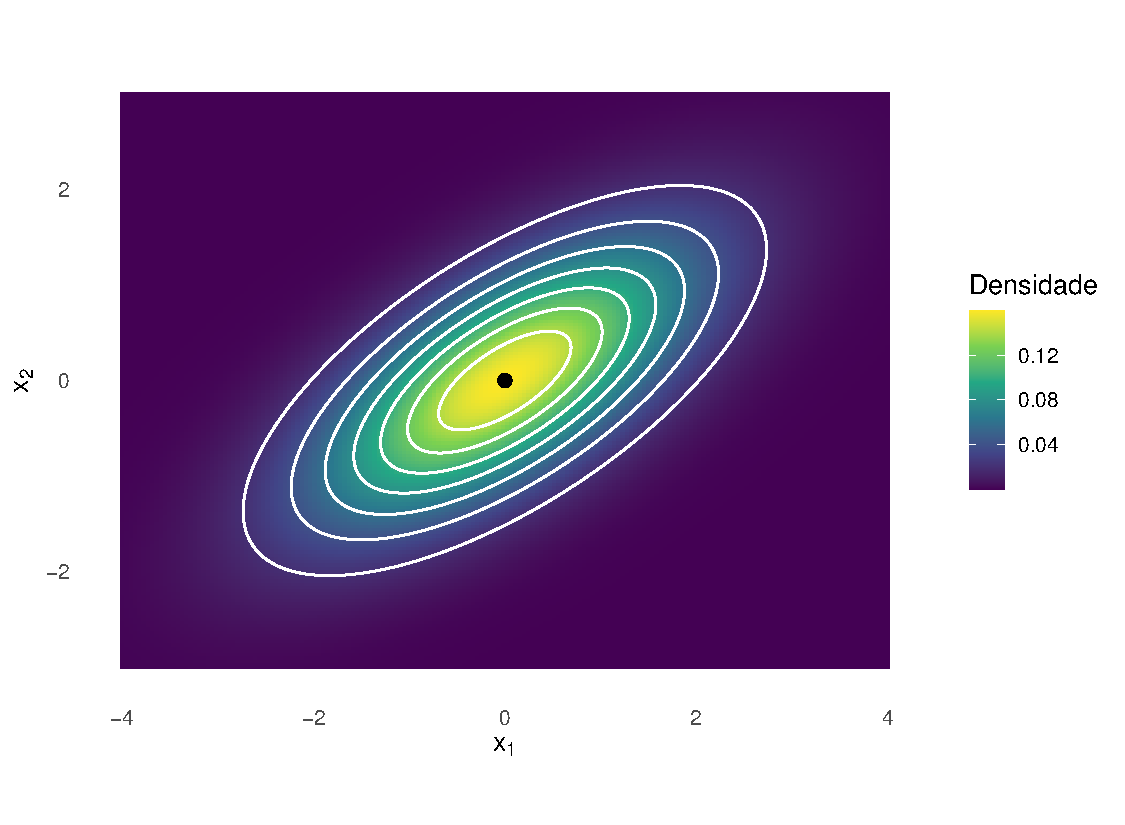
\includegraphics[keepaspectratio]{mod_2_normal_files/figure-pdf/fig-densidade-normal-bivariada-1.pdf}}

}

\caption{\label{fig-densidade-normal-bivariada}Mapa de densidade e
curvas de nível de uma distribuição normal bivariada.}

\end{figure}%

As curvas de nível são elipses centradas em \(\boldsymbol{\mu}\). Todos
os pontos sobre uma mesma curva apresentam a mesma distância de
Mahalanobis ao centro e, consequentemente, a mesma densidade.

A região interna correspondente é

\begin{equation}\phantomsection\label{eq-regiao-elipsoidal-normal}{
\mathcal E_c
=
\left\{
\mathbf x\in\mathbb{R}^p:
d_M^2
\left(
\mathbf x,
\boldsymbol{\mu}
\right)
\leq
c
\right\}.
}\end{equation}

Neste ponto, \(c\) é apenas uma constante positiva. Mais adiante, a
distribuição de \(D_M^2\) permitirá escolher valores de \(c\) associados
a probabilidades populacionais específicas.

\section{Transformações e distribuições
marginais}\label{transformauxe7uxf5es-e-distribuiuxe7uxf5es-marginais}

A construção na Proposição~\ref{prp-construcao-afim-normal} partiu de um
vetor normal padrão. Uma propriedade mais geral da família normal é o
fechamento sob transformações afins. Essa propriedade permite obter
distribuições de combinações lineares, projeções, subvectores e
transformações de padronização sem recalcular densidades por integração.

\subsection{Fechamento sob transformações
afins}\label{fechamento-sob-transformauxe7uxf5es-afins}

Considere

\[
\boldsymbol{\mathsf X}
\sim
N_p
\left(
\boldsymbol{\mu},
\boldsymbol{\Sigma}
\right),
\]

\(\mathbf A\in\mathbb{R}^{m\times p}\) e \(\mathbf b\in\mathbb{R}^m\).

\begin{proposition}[Fechamento da família normal sob transformações
afins]\protect\hypertarget{prp-transformacao-afim-normal}{}\label{prp-transformacao-afim-normal}

Se

\[
\boldsymbol{\mathsf X}
\sim
N_p
\left(
\boldsymbol{\mu},
\boldsymbol{\Sigma}
\right),
\]

a transformação afim

\begin{equation}\phantomsection\label{eq-transformacao-afim-vetor-normal}{
\boldsymbol{\mathsf Y}
=
\mathbf A
\boldsymbol{\mathsf X}
+
\mathbf b
}\end{equation}

satisfaz

\begin{equation}\phantomsection\label{eq-distribuicao-transformacao-afim-normal}{
\boldsymbol{\mathsf Y}
\sim
N_m
\left(
\mathbf A
\boldsymbol{\mu}
+
\mathbf b,
\mathbf A
\boldsymbol{\Sigma}
\mathbf A^\top
\right),
}\end{equation}

em que

\[
\mathbf A
\in
\mathbb R^{m\times p}
\qquad
\text{e}
\qquad
\mathbf b
\in
\mathbb R^m.
\]

\end{proposition}

\begin{proof}
Pela Proposição~\ref{prp-transformacao-afim-covariancia},

\[
E
\left(
\boldsymbol{\mathsf Y}
\right)
=
\mathbf A
\boldsymbol{\mu}
+
\mathbf b
\]

e

\[
\operatorname{Cov}
\left(
\boldsymbol{\mathsf Y}
\right)
=
\mathbf A
\boldsymbol{\Sigma}
\mathbf A^\top.
\]

Para qualquer \(\mathbf c\in\mathbb{R}^m\),

\[
\begin{aligned}
\mathbf c^\top
\boldsymbol{\mathsf Y}
&=
\mathbf c^\top
\left(
\mathbf A
\boldsymbol{\mathsf X}
+
\mathbf b
\right)\\
&=
\left(
\mathbf A^\top
\mathbf c
\right)^\top
\boldsymbol{\mathsf X}
+
\mathbf c^\top
\mathbf b.
\end{aligned}
\]

Como \(\boldsymbol{\mathsf X}\) é normal multivariado,

\[
\left(
\mathbf A^\top
\mathbf c
\right)^\top
\boldsymbol{\mathsf X}
\]

é normal. A adição de uma constante preserva a normalidade. Portanto,
toda combinação linear das componentes de \(\boldsymbol{\mathsf Y}\) é
normal, o que demonstra o resultado.
\end{proof}

As fórmulas para média e covariância são válidas para vetores aleatórios
gerais com segundos momentos finitos. O resultado específico da família
normal é o \textbf{fechamento distribucional}: se
\(\boldsymbol{\mathsf X}\) possui distribuição normal multivariada,
então \(\mathbf A\boldsymbol{\mathsf X}+\mathbf b\) também possui
distribuição normal multivariada.

A matriz \(\mathbf A\) não precisa possuir posto completo.
Consequentemente, a matriz de covariâncias transformada

\[
\mathbf A
\boldsymbol{\Sigma}
\mathbf A^\top
\]

pode não ser positiva definida. Esse caso será retomado em
Seção~\ref{sec-normal-singular}.

\begin{example}[Transformação de um vetor normal
bivariado]\protect\hypertarget{exm-transformacao-afim-normal}{}\label{exm-transformacao-afim-normal}

Considere

\[
\boldsymbol{\mathsf X}
=
\begin{bmatrix}
X_1\\
X_2
\end{bmatrix}
\sim
N_2
\left(
\begin{bmatrix}
2\\
1
\end{bmatrix},
\begin{bmatrix}
4 & 1\\
1 & 2
\end{bmatrix}
\right).
\]

Defina

\[
\boldsymbol{\mathsf Y}
=
\begin{bmatrix}
Y_1\\
Y_2
\end{bmatrix}
=
\begin{bmatrix}
1 & 1\\
1 & -1
\end{bmatrix}
\boldsymbol{\mathsf X}
+
\begin{bmatrix}
0\\
3
\end{bmatrix}.
\]

Logo,

\[
Y_1
=
X_1+X_2
\]

e

\[
Y_2
=
X_1-X_2+3.
\]

O vetor de médias é

\[
\begin{aligned}
E
\left(
\boldsymbol{\mathsf Y}
\right)
&=
\begin{bmatrix}
1 & 1\\
1 & -1
\end{bmatrix}
\begin{bmatrix}
2\\
1
\end{bmatrix}
+
\begin{bmatrix}
0\\
3
\end{bmatrix}\\
&=
\begin{bmatrix}
3\\
4
\end{bmatrix},
\end{aligned}
\]

e a matriz de covariâncias é

\[
\begin{aligned}
\operatorname{Cov}
\left(
\boldsymbol{\mathsf Y}
\right)
&=
\begin{bmatrix}
1 & 1\\
1 & -1
\end{bmatrix}
\begin{bmatrix}
4 & 1\\
1 & 2
\end{bmatrix}
\begin{bmatrix}
1 & 1\\
1 & -1
\end{bmatrix}\\
&=
\begin{bmatrix}
8 & 2\\
2 & 4
\end{bmatrix}.
\end{aligned}
\]

Portanto,

\[
\boldsymbol{\mathsf Y}
\sim
N_2
\left(
\begin{bmatrix}
3\\
4
\end{bmatrix},
\begin{bmatrix}
8 & 2\\
2 & 4
\end{bmatrix}
\right).
\]

O exemplo mostra que uma transformação afim modifica simultaneamente
localização e covariância, mas preserva a família normal.

\end{example}

\subsection{Combinações lineares}\label{combinauxe7uxf5es-lineares-1}

Uma combinação linear é o caso \(m=1\) de
Proposição~\ref{prp-transformacao-afim-normal}.

Para \(\mathbf a\in\mathbb{R}^p\) e \(b\in\mathbb{R}\),

\[
Y
=
\mathbf a^\top
\boldsymbol{\mathsf X}
+
b
\]

satisfaz

\begin{equation}\phantomsection\label{eq-distribuicao-combinacao-linear-normal}{
Y
\sim
N
\left(
\mathbf a^\top
\boldsymbol{\mu}
+
b,
\mathbf a^\top
\boldsymbol{\Sigma}
\mathbf a
\right).
}\end{equation}

A expressão fornece diretamente a distribuição de somas, diferenças,
contrastes, médias ponderadas e projeções lineares.

\begin{example}[Soma e diferença de componentes conjuntamente
normais]\protect\hypertarget{exm-soma-diferenca-normais}{}\label{exm-soma-diferenca-normais}

Considere

\[
\begin{bmatrix}
X_1\\
X_2
\end{bmatrix}
\sim
N_2
\left(
\begin{bmatrix}
\mu_1\\
\mu_2
\end{bmatrix},
\begin{bmatrix}
\sigma_1^2 & \sigma_{12}\\
\sigma_{12} & \sigma_2^2
\end{bmatrix}
\right).
\]

Para

\[
Y_1
=
X_1+X_2,
\]

tem-se

\[
Y_1
\sim
N
\left(
\mu_1+\mu_2,
\sigma_1^2
+
\sigma_2^2
+
2\sigma_{12}
\right).
\]

Para

\[
Y_2
=
X_1-X_2,
\]

tem-se

\[
Y_2
\sim
N
\left(
\mu_1-\mu_2,
\sigma_1^2
+
\sigma_2^2
-
2\sigma_{12}
\right).
\]

Quando \(\sigma_{12}>0\), a covariância aumenta a variância da soma e
reduz a variância da diferença. Para \(\sigma_{12}<0\), ocorre o efeito
inverso.

\end{example}

Se

\[
\mathbf a^\top
\boldsymbol{\Sigma}
\mathbf a
=
0,
\]

então

\[
\mathbf a^\top
\boldsymbol{\mathsf X}
+
b
=
\mathbf a^\top
\boldsymbol{\mu}
+
b
\]

quase certamente.

\subsection{Distribuições
marginais}\label{distribuiuxe7uxf5es-marginais-1}

As distribuições marginais de subvectores também podem ser obtidas como
transformações lineares.

Considere

\begin{equation}\phantomsection\label{eq-particionamento-normal}{
\boldsymbol{\mathsf X}
=
\begin{bmatrix}
\boldsymbol{\mathsf X}_1\\
\boldsymbol{\mathsf X}_2
\end{bmatrix}
\sim
N_p
\left(
\begin{bmatrix}
\boldsymbol{\mu}_1\\
\boldsymbol{\mu}_2
\end{bmatrix},
\begin{bmatrix}
\boldsymbol{\Sigma}_{11}
&
\boldsymbol{\Sigma}_{12}\\
\boldsymbol{\Sigma}_{21}
&
\boldsymbol{\Sigma}_{22}
\end{bmatrix}
\right),
}\end{equation}

em que

\[
\boldsymbol{\mathsf X}_1
\in
\mathbb{R}^{p_1},
\qquad
\boldsymbol{\mathsf X}_2
\in
\mathbb{R}^{p_2},
\qquad
p_1+p_2=p.
\]

\begin{proposition}[Distribuições marginais da normal
multivariada]\protect\hypertarget{prp-marginais-normal}{}\label{prp-marginais-normal}

Os blocos marginais de um vetor normal multivariado particionado
satisfazem

\begin{equation}\phantomsection\label{eq-marginal-primeiro-bloco}{
\boldsymbol{\mathsf X}_1
\sim
N_{p_1}
\left(
\boldsymbol{\mu}_1,
\boldsymbol{\Sigma}_{11}
\right)
}\end{equation}

e

\begin{equation}\phantomsection\label{eq-marginal-segundo-bloco}{
\boldsymbol{\mathsf X}_2
\sim
N_{p_2}
\left(
\boldsymbol{\mu}_2,
\boldsymbol{\Sigma}_{22}
\right).
}\end{equation}

Esse resultado considera a estrutura conjunta

\[
\begin{bmatrix}
\boldsymbol{\mathsf X}_1\\
\boldsymbol{\mathsf X}_2
\end{bmatrix}
\sim
N_p
\left(
\begin{bmatrix}
\boldsymbol{\mu}_1\\
\boldsymbol{\mu}_2
\end{bmatrix},
\begin{bmatrix}
\boldsymbol{\Sigma}_{11}
&
\boldsymbol{\Sigma}_{12}\\
\boldsymbol{\Sigma}_{21}
&
\boldsymbol{\Sigma}_{22}
\end{bmatrix}
\right),
\]

em que

\[
\boldsymbol{\mathsf X}_1
\in
\mathbb R^{p_1},
\qquad
\boldsymbol{\mathsf X}_2
\in
\mathbb R^{p_2},
\qquad
p_1+p_2=p.
\]

\end{proposition}

\begin{proof}
O primeiro bloco pode ser escrito como

\[
\boldsymbol{\mathsf X}_1
=
\mathbf A_1
\boldsymbol{\mathsf X},
\]

com

\[
\mathbf A_1
=
\begin{bmatrix}
\mathbf I_{p_1}
&
\mathbf 0
\end{bmatrix}.
\]

Pela Proposição~\ref{prp-transformacao-afim-normal},

\[
\boldsymbol{\mathsf X}_1
\sim
N_{p_1}
\left(
\mathbf A_1\boldsymbol{\mu},
\mathbf A_1
\boldsymbol{\Sigma}
\mathbf A_1^\top
\right).
\]

A estrutura particionada fornece

\[
\mathbf A_1
\boldsymbol{\mu}
=
\boldsymbol{\mu}_1
\]

e

\[
\mathbf A_1
\boldsymbol{\Sigma}
\mathbf A_1^\top
=
\boldsymbol{\Sigma}_{11}.
\]

O segundo bloco é obtido de forma análoga.
\end{proof}

A distribuição marginal de um bloco depende de seu vetor de médias e de
sua própria matriz de covariâncias. A matriz
\(\boldsymbol{\Sigma}_{12}\) não aparece nos parâmetros marginais, mas
participa da estrutura de dependência conjunta.

\begin{example}[Marginal de um vetor normal
trivariado]\protect\hypertarget{exm-normal-marginal}{}\label{exm-normal-marginal}

Considere

\[
\boldsymbol{\mathsf X}
=
\begin{bmatrix}
X_1\\
X_2\\
X_3
\end{bmatrix}
\sim
N_3
\left(
\begin{bmatrix}
1\\
2\\
0
\end{bmatrix},
\begin{bmatrix}
4 & 1 & -1\\
1 & 3 & 0,5\\
-1 & 0,5 & 2
\end{bmatrix}
\right).
\]

Selecionando \(X_1\) e \(X_3\),

\[
\begin{bmatrix}
X_1\\
X_3
\end{bmatrix}
\sim
N_2
\left(
\begin{bmatrix}
1\\
0
\end{bmatrix},
\begin{bmatrix}
4 & -1\\
-1 & 2
\end{bmatrix}
\right).
\]

A média marginal é formada pelas componentes correspondentes de
\(\boldsymbol{\mu}\), e a matriz de covariâncias marginal é a submatriz
principal associada às variáveis selecionadas.

\end{example}

\subsection{Padronização marginal e
branqueamento}\label{padronizauxe7uxe3o-marginal-e-branqueamento}

O Capítulo 8 definiu na Equação~\ref{eq-matriz-variancias-populacionais}
a matriz

\[
\mathbf D_{\Sigma}
=
\operatorname{diag}
\left(
\sigma_{11},\ldots,\sigma_{pp}
\right).
\]

Suponha

\[
\sigma_{jj}>0,
\qquad
j=1,\ldots,p.
\]

A padronização marginal é

\begin{equation}\phantomsection\label{eq-padronizacao-marginal-normal}{
\boldsymbol{\mathsf Z}_{\mathrm{pad}}
=
\mathbf D_{\Sigma}^{-1/2}
\left(
\boldsymbol{\mathsf X}
-
\boldsymbol{\mu}
\right).
}\end{equation}

Pela Proposição~\ref{prp-transformacao-afim-normal} e pela definição de
\(\boldsymbol{\mathcal R}\) na
Definição~\ref{def-matriz-correlacoes-populacional},

\begin{equation}\phantomsection\label{eq-distribuicao-vetor-padronizado-normal}{
\boldsymbol{\mathsf Z}_{\mathrm{pad}}
\sim
N_p
\left(
\mathbf 0,
\boldsymbol{\mathcal R}
\right),
}\end{equation}

com

\[
\boldsymbol{\mathcal R}
=
\mathbf D_{\Sigma}^{-1/2}
\boldsymbol{\Sigma}
\mathbf D_{\Sigma}^{-1/2}.
\]

Cada componente padronizada satisfaz

\[
Z_{\mathrm{pad},j}
\sim
N(0,1),
\]

mas as componentes não são necessariamente independentes.

\begin{tcolorbox}[enhanced jigsaw, colback=white, breakable, bottomrule=.15mm, left=2mm, arc=.35mm, rightrule=.15mm, colframe=quarto-callout-caution-color-frame, toprule=.15mm, leftrule=.75mm, opacityback=0]

\vspace{-3mm}\textbf{Padronização não implica independência}\vspace{3mm}

A padronização marginal produz componentes com média zero e variância
unitária, mas preserva as correlações existentes entre elas.

Assim,

\[
\boldsymbol{\mathsf Z}_{\mathrm{pad}}
\sim
N_p
\left(
\mathbf 0,
\boldsymbol{\mathcal R}
\right).
\]

As componentes serão independentes precisamente quando

\[
\boldsymbol{\mathcal R}
=
\mathbf I_p,
\]

resultado que será formalizado na seção seguinte.

\end{tcolorbox}

Quando

\[
\boldsymbol{\Sigma}
\succ
\mathbf 0,
\]

o Capítulo 8 mostrou na Equação~\ref{eq-covariancia-vetor-branqueado}
que o branqueamento simétrico transforma a estrutura de segunda ordem em
covariância identidade. Sob normalidade multivariada, é possível
determinar também a distribuição completa do vetor transformado.

O branqueamento simétrico é dado por

\begin{equation}\phantomsection\label{eq-branqueamento-normal}{
\boldsymbol{\mathsf Z}
=
\boldsymbol{\Sigma}^{-1/2}
\left(
\boldsymbol{\mathsf X}
-
\boldsymbol{\mu}
\right).
}\end{equation}

Pelo fechamento da família normal,

\begin{equation}\phantomsection\label{eq-distribuicao-vetor-branqueado}{
\begin{aligned}
\boldsymbol{\mathsf Z}
&\sim
N_p
\left(
\mathbf 0,
\boldsymbol{\Sigma}^{-1/2}
\boldsymbol{\Sigma}
\boldsymbol{\Sigma}^{-1/2}
\right)\\
&=
N_p
\left(
\mathbf 0,
\mathbf I_p
\right).
\end{aligned}
}\end{equation}

A diferença entre as duas transformações é, portanto,

\[
\mathbf D_{\Sigma}^{-1/2}
\left(
\boldsymbol{\mathsf X}
-
\boldsymbol{\mu}
\right)
\sim
N_p
\left(
\mathbf 0,
\boldsymbol{\mathcal R}
\right)
\]

e

\[
\boldsymbol{\Sigma}^{-1/2}
\left(
\boldsymbol{\mathsf X}
-
\boldsymbol{\mu}
\right)
\sim
N_p
\left(
\mathbf 0,
\mathbf I_p
\right).
\]

A padronização marginal transforma as variâncias em um e preserva as
correlações. O branqueamento transforma toda a matriz de covariâncias em
identidade.

A consequência adicional da normalidade conjunta é probabilística: como
será formalizado na seção seguinte, uma matriz de covariâncias diagonal
implica independência das componentes dentro de um vetor conjuntamente
normal. Portanto, as componentes do vetor branqueado são independentes.

Como discutido no Capítulo 8, o branqueamento não é único. No caso
normal, essa não unicidade preserva também a distribuição normal padrão.
Se \(\mathbf Q_0\) é ortogonal, então

\[
\mathbf Q_0
\boldsymbol{\Sigma}^{-1/2}
\left(
\boldsymbol{\mathsf X}
-
\boldsymbol{\mu}
\right)
\sim
N_p
\left(
\mathbf 0,
\mathbf I_p
\right),
\]

pois

\[
\mathbf Q_0
\mathbf I_p
\mathbf Q_0^\top
=
\mathbf I_p.
\]

O branqueamento simétrico constitui uma escolha específica entre
transformações que produzem covariância identidade.

A próxima seção utiliza uma propriedade específica da normalidade
conjunta: para blocos pertencentes ao mesmo vetor normal multivariado,
covariância cruzada nula é equivalente à independência.

\section{Independência e distribuições
condicionais}\label{independuxeancia-e-distribuiuxe7uxf5es-condicionais}

Quando os segundos momentos existem, a independência entre dois blocos
implica covariância cruzada nula. A implicação inversa, entretanto, não
é válida sem hipóteses adicionais. Na família normal multivariada, a
normalidade conjunta estabelece a equivalência entre independência e
covariância cruzada nula.

A normalidade conjunta também permite determinar a distribuição
condicional de um bloco a partir da estrutura de covariâncias. Nesse
desenvolvimento, o complemento de Schur, definido na
Definição~\ref{def-complemento-schur} e aplicado à matriz de
covariâncias no Capítulo 8, passa a ter uma interpretação
probabilística: ele corresponde à matriz de covariâncias condicional.

\subsection{Independência entre blocos conjuntamente
normais}\label{independuxeancia-entre-blocos-conjuntamente-normais}

Considere o vetor particionado

\begin{equation}\phantomsection\label{eq-particionamento-independencia-normal}{
\boldsymbol{\mathsf X}
=
\begin{bmatrix}
\boldsymbol{\mathsf X}_1\\
\boldsymbol{\mathsf X}_2
\end{bmatrix}
\sim
N_p
\left(
\begin{bmatrix}
\boldsymbol{\mu}_1\\
\boldsymbol{\mu}_2
\end{bmatrix},
\begin{bmatrix}
\boldsymbol{\Sigma}_{11}
&
\boldsymbol{\Sigma}_{12}\\
\boldsymbol{\Sigma}_{21}
&
\boldsymbol{\Sigma}_{22}
\end{bmatrix}
\right),
}\end{equation}

em que

\[
\boldsymbol{\mathsf X}_1
\in
\mathbb{R}^{p_1},
\qquad
\boldsymbol{\mathsf X}_2
\in
\mathbb{R}^{p_2},
\qquad
p_1+p_2=p.
\]

Se os dois blocos são independentes, então

\[
\operatorname{Cov}
\left(
\boldsymbol{\mathsf X}_1,
\boldsymbol{\mathsf X}_2
\right)
=
\boldsymbol{\Sigma}_{12}
=
\mathbf 0.
\]

Essa implicação vale para quaisquer vetores aleatórios independentes com
segundos momentos finitos. A normalidade conjunta permite estabelecer
também a implicação inversa.

Nesta seção, quando o símbolo \(\perp\) aparece entre vetores
aleatórios, a notação

\[
\boldsymbol{\mathsf X}_1
\perp
\boldsymbol{\mathsf X}_2
\]

significa que \(\boldsymbol{\mathsf X}_1\) e
\(\boldsymbol{\mathsf X}_2\) são \textbf{independentes}. Esse uso deve
ser distinguido da ortogonalidade geométrica, também representada pelo
símbolo \(\perp\) nos capítulos de Álgebra Linear.

\begin{proposition}[Independência de blocos conjuntamente
normais]\protect\hypertarget{prp-independencia-blocos-normais}{}\label{prp-independencia-blocos-normais}

Para dois blocos conjuntamente normais,

\[
\boldsymbol{\mathsf X}_1
\perp
\boldsymbol{\mathsf X}_2
\]

se, e somente se,

\begin{equation}\phantomsection\label{eq-independencia-covariancia-blocos-normais}{
\boldsymbol{\Sigma}_{12}
=
\mathbf0,
}\end{equation}

considerando a estrutura conjunta

\[
\begin{bmatrix}
\boldsymbol{\mathsf X}_1\\
\boldsymbol{\mathsf X}_2
\end{bmatrix}
\sim
N_p
\left(
\begin{bmatrix}
\boldsymbol{\mu}_1\\
\boldsymbol{\mu}_2
\end{bmatrix},
\begin{bmatrix}
\boldsymbol{\Sigma}_{11}
&
\boldsymbol{\Sigma}_{12}\\
\boldsymbol{\Sigma}_{21}
&
\boldsymbol{\Sigma}_{22}
\end{bmatrix}
\right),
\]

em que

\[
\boldsymbol{\mathsf X}_1
\in
\mathbb R^{p_1},
\qquad
\boldsymbol{\mathsf X}_2
\in
\mathbb R^{p_2},
\qquad
p_1+p_2=p,
\]

e

\[
\boldsymbol{\Sigma}_{12}
=
\operatorname{Cov}
\left(
\boldsymbol{\mathsf X}_1,
\boldsymbol{\mathsf X}_2
\right).
\]

\end{proposition}

\begin{proof}
Se

\[
\boldsymbol{\mathsf X}_1
\perp
\boldsymbol{\mathsf X}_2,
\]

então a independência implica

\[
\boldsymbol{\Sigma}_{12}
=
\operatorname{Cov}
\left(
\boldsymbol{\mathsf X}_1,
\boldsymbol{\mathsf X}_2
\right)
=
\mathbf 0.
\]

Para a implicação inversa, suponha

\[
\boldsymbol{\Sigma}_{12}
=
\mathbf 0.
\]

Como

\[
\boldsymbol{\Sigma}_{21}
=
\boldsymbol{\Sigma}_{12}^\top,
\]

a matriz de covariâncias conjunta assume a forma

\[
\boldsymbol{\Sigma}
=
\begin{bmatrix}
\boldsymbol{\Sigma}_{11}
&
\mathbf 0\\
\mathbf 0
&
\boldsymbol{\Sigma}_{22}
\end{bmatrix}.
\]

Existem matrizes \(\mathbf A_1\) e \(\mathbf A_2\) tais que

\[
\boldsymbol{\Sigma}_{11}
=
\mathbf A_1\mathbf A_1^\top
\]

e

\[
\boldsymbol{\Sigma}_{22}
=
\mathbf A_2\mathbf A_2^\top.
\]

Considere vetores normais padrão independentes
\(\boldsymbol{\mathsf Z}_1\) e \(\boldsymbol{\mathsf Z}_2\) e defina

\[
\boldsymbol{\mathsf Y}_1
=
\boldsymbol{\mu}_1
+
\mathbf A_1
\boldsymbol{\mathsf Z}_1
\]

e

\[
\boldsymbol{\mathsf Y}_2
=
\boldsymbol{\mu}_2
+
\mathbf A_2
\boldsymbol{\mathsf Z}_2.
\]

Por construção,

\[
\boldsymbol{\mathsf Y}_1
\perp
\boldsymbol{\mathsf Y}_2.
\]

Além disso,

\[
\begin{bmatrix}
\boldsymbol{\mathsf Y}_1\\
\boldsymbol{\mathsf Y}_2
\end{bmatrix}
\sim
N_p
\left(
\begin{bmatrix}
\boldsymbol{\mu}_1\\
\boldsymbol{\mu}_2
\end{bmatrix},
\begin{bmatrix}
\boldsymbol{\Sigma}_{11}
&
\mathbf 0\\
\mathbf 0
&
\boldsymbol{\Sigma}_{22}
\end{bmatrix}
\right).
\]

Pela Proposição~\ref{prp-determinacao-normal-parametros},

\[
\begin{bmatrix}
\boldsymbol{\mathsf X}_1\\
\boldsymbol{\mathsf X}_2
\end{bmatrix}
\overset{d}{=}
\begin{bmatrix}
\boldsymbol{\mathsf Y}_1\\
\boldsymbol{\mathsf Y}_2
\end{bmatrix}.
\]

Portanto,

\[
\boldsymbol{\mathsf X}_1
\perp
\boldsymbol{\mathsf X}_2.
\]
\end{proof}

Como caso particular, se

\[
\boldsymbol{\mathsf X}
\sim
N_p
\left(
\boldsymbol{\mu},
\boldsymbol{\Sigma}
\right)
\]

e \(\boldsymbol{\Sigma}\) é diagonal, então

\[
X_1,\ldots,X_p
\]

são mutuamente independentes.

Esse resultado é uma consequência específica da normalidade conjunta.
Sem essa hipótese, uma matriz de covariâncias diagonal garante
covariância nula entre componentes, mas não implica independência.

\begin{tcolorbox}[enhanced jigsaw, colback=white, breakable, bottomrule=.15mm, left=2mm, arc=.35mm, rightrule=.15mm, colframe=quarto-callout-caution-color-frame, toprule=.15mm, leftrule=.75mm, opacityback=0]

\vspace{-3mm}\textbf{A normalidade deve ser conjunta}\vspace{3mm}

A equivalência

\[
\operatorname{Cov}(X_i,X_j)=0
\quad\Longleftrightarrow\quad
X_i\perp X_j
\]

exige que \(X_i\) e \(X_j\) pertençam ao mesmo vetor normal
multivariado.

A normalidade de cada variável considerada separadamente não é
suficiente para essa conclusão.

\end{tcolorbox}

\subsection{Distribuição
condicional}\label{distribuiuxe7uxe3o-condicional}

Considere novamente

\[
\boldsymbol{\mathsf X}
=
\begin{bmatrix}
\boldsymbol{\mathsf X}_1\\
\boldsymbol{\mathsf X}_2
\end{bmatrix}
\sim
N_p
\left(
\begin{bmatrix}
\boldsymbol{\mu}_1\\
\boldsymbol{\mu}_2
\end{bmatrix},
\begin{bmatrix}
\boldsymbol{\Sigma}_{11}
&
\boldsymbol{\Sigma}_{12}\\
\boldsymbol{\Sigma}_{21}
&
\boldsymbol{\Sigma}_{22}
\end{bmatrix}
\right),
\]

e suponha

\[
\boldsymbol{\Sigma}
\succ
\mathbf0.
\]

Como \(\boldsymbol{\Sigma}_{22}\) é uma submatriz principal de uma
matriz positiva definida,

\[
\boldsymbol{\Sigma}_{22}
\succ
\mathbf0,
\]

de modo que \(\boldsymbol{\Sigma}_{22}^{-1}\) existe.

Na notação condicional, a barra vertical \(\mid\) deve ser lida como
\textbf{dado}. Assim,

\[
\boldsymbol{\mathsf X}_1
\mid
\boldsymbol{\mathsf X}_2
=
\mathbf x_2
\]

representa o vetor \(\boldsymbol{\mathsf X}_1\) condicionado ao valor
\(\boldsymbol{\mathsf X}_2=\mathbf x_2\), e o subscrito \(1\mid2\) será
utilizado para identificar quantidades condicionais relativas ao
primeiro bloco dado o segundo.

\begin{proposition}[Distribuição condicional da normal
multivariada]\protect\hypertarget{prp-distribuicao-condicional-normal}{}\label{prp-distribuicao-condicional-normal}

A distribuição condicional de um bloco de um vetor normal multivariado
particionado é normal multivariada:

\begin{equation}\phantomsection\label{eq-distribuicao-condicional-normal}{
\boldsymbol{\mathsf X}_1
\mid
\boldsymbol{\mathsf X}_2
=
\mathbf x_2
\sim
N_{p_1}
\left(
\boldsymbol{\mu}_{1\mid2}
\left(
\mathbf x_2
\right),
\boldsymbol{\Sigma}_{11\cdot2}
\right).
}\end{equation}

Esse resultado considera a estrutura conjunta

\[
\begin{bmatrix}
\boldsymbol{\mathsf X}_1\\
\boldsymbol{\mathsf X}_2
\end{bmatrix}
\sim
N_p
\left(
\begin{bmatrix}
\boldsymbol{\mu}_1\\
\boldsymbol{\mu}_2
\end{bmatrix},
\begin{bmatrix}
\boldsymbol{\Sigma}_{11}
&
\boldsymbol{\Sigma}_{12}\\
\boldsymbol{\Sigma}_{21}
&
\boldsymbol{\Sigma}_{22}
\end{bmatrix}
\right),
\]

em que

\[
\boldsymbol{\mathsf X}_1
\in
\mathbb R^{p_1},
\qquad
\boldsymbol{\mathsf X}_2
\in
\mathbb R^{p_2},
\qquad
\mathbf x_2
\in
\mathbb R^{p_2},
\qquad
p_1+p_2=p,
\]

e

\[
\boldsymbol{\Sigma}_{22}
\succ
\mathbf0.
\]

A média condicional é

\begin{equation}\phantomsection\label{eq-media-condicional-normal}{
\boldsymbol{\mu}_{1\mid2}
\left(
\mathbf x_2
\right)
=
\boldsymbol{\mu}_1
+
\boldsymbol{\Sigma}_{12}
\boldsymbol{\Sigma}_{22}^{-1}
\left(
\mathbf x_2-\boldsymbol{\mu}_2
\right)
}\end{equation}

e a matriz de covariâncias condicional é

\begin{equation}\phantomsection\label{eq-covariancia-condicional-normal}{
\boldsymbol{\Sigma}_{11\cdot2}
=
\boldsymbol{\Sigma}_{11}
-
\boldsymbol{\Sigma}_{12}
\boldsymbol{\Sigma}_{22}^{-1}
\boldsymbol{\Sigma}_{21}.
}\end{equation}

A matriz \(\boldsymbol{\Sigma}_{11\cdot2}\) é o complemento de Schur de
\(\boldsymbol{\Sigma}_{22}\) em \(\boldsymbol{\Sigma}\), definido em
Equação~\ref{eq-complemento-schur-covariancia}.

\end{proposition}

\begin{proof}
Considere

\[
\mathbf L^\star
=
\boldsymbol{\Sigma}_{12}
\boldsymbol{\Sigma}_{22}^{-1}
\]

e defina o vetor residual

\begin{equation}\phantomsection\label{eq-residuo-condicional-normal}{
\boldsymbol{\mathsf E}_{1\mid2}
=
\boldsymbol{\mathsf X}_1
-
\boldsymbol{\mu}_1
-
\mathbf L^\star
\left(
\boldsymbol{\mathsf X}_2
-
\boldsymbol{\mu}_2
\right).
}\end{equation}

Os vetores \(\boldsymbol{\mathsf E}_{1\mid2}\) e
\(\boldsymbol{\mathsf X}_2\) são obtidos conjuntamente por uma
transformação afim de \(\boldsymbol{\mathsf X}\). Pela
Proposição~\ref{prp-transformacao-afim-normal},

\[
\begin{bmatrix}
\boldsymbol{\mathsf E}_{1\mid2}\\
\boldsymbol{\mathsf X}_2
\end{bmatrix}
\]

possui distribuição normal multivariada.

A covariância cruzada entre o resíduo e o bloco condicionante é

\[
\begin{aligned}
\operatorname{Cov}
\left(
\boldsymbol{\mathsf E}_{1\mid2},
\boldsymbol{\mathsf X}_2
\right)
&=
\boldsymbol{\Sigma}_{12}
-
\mathbf L^\star
\boldsymbol{\Sigma}_{22}\\
&=
\boldsymbol{\Sigma}_{12}
-
\boldsymbol{\Sigma}_{12}
\boldsymbol{\Sigma}_{22}^{-1}
\boldsymbol{\Sigma}_{22}\\
&=
\mathbf 0.
\end{aligned}
\]

Pela Proposição~\ref{prp-independencia-blocos-normais},

\begin{equation}\phantomsection\label{eq-independencia-residuo-condicionante}{
\boldsymbol{\mathsf E}_{1\mid2}
\perp
\boldsymbol{\mathsf X}_2.
}\end{equation}

Além disso,

\[
E
\left(
\boldsymbol{\mathsf E}_{1\mid2}
\right)
=
\mathbf 0.
\]

Pela Proposição~\ref{prp-complemento-schur-covariancia-residual},

\[
\begin{aligned}
\operatorname{Cov}
\left(
\boldsymbol{\mathsf E}_{1\mid2}
\right)
&=
\boldsymbol{\Sigma}_{11}
-
\boldsymbol{\Sigma}_{12}
\boldsymbol{\Sigma}_{22}^{-1}
\boldsymbol{\Sigma}_{21}\\
&=
\boldsymbol{\Sigma}_{11\cdot2}.
\end{aligned}
\]

Portanto,

\[
\boldsymbol{\mathsf E}_{1\mid2}
\sim
N_{p_1}
\left(
\mathbf 0,
\boldsymbol{\Sigma}_{11\cdot2}
\right).
\]

Reorganizando Equação~\ref{eq-residuo-condicional-normal},

\[
\boldsymbol{\mathsf X}_1
=
\boldsymbol{\mu}_1
+
\boldsymbol{\Sigma}_{12}
\boldsymbol{\Sigma}_{22}^{-1}
\left(
\boldsymbol{\mathsf X}_2-\boldsymbol{\mu}_2
\right)
+
\boldsymbol{\mathsf E}_{1\mid2}.
\]

Condicionando em

\[
\boldsymbol{\mathsf X}_2
=
\mathbf x_2,
\]

a parcela que depende de \(\boldsymbol{\mathsf X}_2\) torna-se

\[
\boldsymbol{\mu}_{1\mid2}
\left(
\mathbf x_2
\right).
\]

Como \(\boldsymbol{\mathsf E}_{1\mid2}\) é independente de
\(\boldsymbol{\mathsf X}_2\), sua distribuição permanece

\[
N_{p_1}
\left(
\mathbf 0,
\boldsymbol{\Sigma}_{11\cdot2}
\right)
\]

após o condicionamento. Portanto,

\[
\boldsymbol{\mathsf X}_1
\mid
\boldsymbol{\mathsf X}_2
=
\mathbf x_2
\sim
N_{p_1}
\left(
\boldsymbol{\mu}_{1\mid2}
\left(
\mathbf x_2
\right),
\boldsymbol{\Sigma}_{11\cdot2}
\right).
\]
\end{proof}

A demonstração fornece a decomposição

\begin{equation}\phantomsection\label{eq-decomposicao-condicional-normal}{
\boldsymbol{\mathsf X}_1
=
\boldsymbol{\mu}_{1\mid2}
\left(
\boldsymbol{\mathsf X}_2
\right)
+
\boldsymbol{\mathsf E}_{1\mid2},
}\end{equation}

com

\[
\boldsymbol{\mathsf E}_{1\mid2}
\perp
\boldsymbol{\mathsf X}_2.
\]

Consequentemente,

\begin{equation}\phantomsection\label{eq-esperanca-condicional-normal}{
E
\left(
\boldsymbol{\mathsf X}_1
\mid
\boldsymbol{\mathsf X}_2
\right)
=
\boldsymbol{\mu}_1
+
\boldsymbol{\Sigma}_{12}
\boldsymbol{\Sigma}_{22}^{-1}
\left(
\boldsymbol{\mathsf X}_2
-
\boldsymbol{\mu}_2
\right).
}\end{equation}

No Capítulo 8, na
Proposição~\ref{prp-complemento-schur-covariancia-residual}, a expressão

\[
\boldsymbol{\mu}_1
+
\boldsymbol{\Sigma}_{12}
\boldsymbol{\Sigma}_{22}^{-1}
\left(
\boldsymbol{\mathsf X}_2
-
\boldsymbol{\mu}_2
\right)
\]

surgiu como o melhor ajuste linear de \(\boldsymbol{\mathsf X}_1\) em
função de \(\boldsymbol{\mathsf X}_2\), utilizando apenas informações de
primeira e segunda ordem.

Sob normalidade conjunta, ocorre um resultado mais forte:

\[
E
\left(
\boldsymbol{\mathsf X}_1
\mid
\boldsymbol{\mathsf X}_2
\right)
=
\boldsymbol{\mu}_1
+
\boldsymbol{\Sigma}_{12}
\boldsymbol{\Sigma}_{22}^{-1}
\left(
\boldsymbol{\mathsf X}_2
-
\boldsymbol{\mu}_2
\right).
\]

Assim, na família normal multivariada, o melhor ajuste linear coincide
exatamente com a esperança condicional, e a matriz de covariâncias do
resíduo linear coincide com a matriz de covariâncias condicional.

\subsection{Média e covariância
condicionais}\label{muxe9dia-e-covariuxe2ncia-condicionais}

A média condicional

\[
\boldsymbol{\mu}_{1\mid2}
\left(
\mathbf x_2
\right)
=
\boldsymbol{\mu}_1
+
\boldsymbol{\Sigma}_{12}
\boldsymbol{\Sigma}_{22}^{-1}
\left(
\mathbf x_2-\boldsymbol{\mu}_2
\right)
\]

depende do valor condicionado.

O vetor

\[
\mathbf x_2
-
\boldsymbol{\mu}_2
\]

representa o afastamento do bloco conhecido em relação à sua média. A
matriz

\[
\boldsymbol{\Sigma}_{12}
\boldsymbol{\Sigma}_{22}^{-1}
\]

transforma esse afastamento em um ajuste para a média de
\(\boldsymbol{\mathsf X}_1\).

Quando

\[
\mathbf x_2
=
\boldsymbol{\mu}_2,
\]

tem-se

\[
\boldsymbol{\mu}_{1\mid2}
\left(
\boldsymbol{\mu}_2
\right)
=
\boldsymbol{\mu}_1.
\]

Quando

\[
\boldsymbol{\Sigma}_{12}
=
\mathbf 0,
\]

a média condicional não depende de \(\mathbf x_2\):

\[
\boldsymbol{\mu}_{1\mid2}
\left(
\mathbf x_2
\right)
=
\boldsymbol{\mu}_1.
\]

A matriz de covariâncias condicional é

\[
\boldsymbol{\Sigma}_{11\cdot2}
=
\boldsymbol{\Sigma}_{11}
-
\boldsymbol{\Sigma}_{12}
\boldsymbol{\Sigma}_{22}^{-1}
\boldsymbol{\Sigma}_{21}.
\]

Ela não depende do valor específico de \(\mathbf x_2\). Assim,
diferentes valores do bloco condicionante deslocam o centro da
distribuição condicional, mas não alteram sua matriz de covariâncias.

Como \(\boldsymbol{\Sigma}\succ\mathbf0\), a propriedade de positividade
do complemento de Schur fornece

\begin{equation}\phantomsection\label{eq-positividade-covariancia-condicional}{
\boldsymbol{\Sigma}_{11\cdot2}
\succ
\mathbf 0.
}\end{equation}

A diferença entre as covariâncias marginal e condicional é

\begin{equation}\phantomsection\label{eq-reducao-covariancia-condicional}{
\boldsymbol{\Sigma}_{11}
-
\boldsymbol{\Sigma}_{11\cdot2}
=
\boldsymbol{\Sigma}_{12}
\boldsymbol{\Sigma}_{22}^{-1}
\boldsymbol{\Sigma}_{21}.
}\end{equation}

Como

\[
\boldsymbol{\Sigma}_{12}
\boldsymbol{\Sigma}_{22}^{-1}
\boldsymbol{\Sigma}_{21}
\succeq
\mathbf 0,
\]

segue que

\begin{equation}\phantomsection\label{eq-ordem-covariancia-condicional}{
\boldsymbol{\Sigma}_{11\cdot2}
\preceq
\boldsymbol{\Sigma}_{11}.
}\end{equation}

Portanto, para qualquer \(\mathbf a\in\mathbb{R}^{p_1}\),

\[
\begin{aligned}
\operatorname{Var}
\left[
\mathbf a^\top
\boldsymbol{\mathsf X}_1
\mid
\boldsymbol{\mathsf X}_2
=
\mathbf x_2
\right]
&=
\mathbf a^\top
\boldsymbol{\Sigma}_{11\cdot2}
\mathbf a\\
&\leq
\mathbf a^\top
\boldsymbol{\Sigma}_{11}
\mathbf a.
\end{aligned}
\]

Condicionar no segundo bloco não aumenta a variância de nenhuma
combinação linear do primeiro bloco.

Quando

\[
\boldsymbol{\Sigma}_{12}
=
\mathbf 0,
\]

tem-se simultaneamente

\[
\boldsymbol{\mu}_{1\mid2}
\left(
\mathbf x_2
\right)
=
\boldsymbol{\mu}_1
\]

e

\[
\boldsymbol{\Sigma}_{11\cdot2}
=
\boldsymbol{\Sigma}_{11}.
\]

Nesse caso, a distribuição condicional coincide com a distribuição
marginal, como consequência da independência entre os blocos
estabelecida na Proposição~\ref{prp-independencia-blocos-normais}.

\subsection{Caso bivariado}\label{caso-bivariado}

Considere

\begin{equation}\phantomsection\label{eq-normal-bivariada-condicional}{
\begin{bmatrix}
X_1\\
X_2
\end{bmatrix}
\sim
N_2
\left(
\begin{bmatrix}
\mu_1\\
\mu_2
\end{bmatrix},
\begin{bmatrix}
\sigma_1^2
&
\rho\sigma_1\sigma_2\\
\rho\sigma_1\sigma_2
&
\sigma_2^2
\end{bmatrix}
\right),
}\end{equation}

com

\[
\sigma_1>0,
\qquad
\sigma_2>0,
\qquad
-1<\rho<1.
\]

A média condicional de \(X_1\) dado \(X_2=x_2\) é

\begin{equation}\phantomsection\label{eq-media-condicional-normal-bivariada}{
\begin{aligned}
E
\left(
X_1
\mid
X_2=x_2
\right)
&=
\mu_1
+
\frac{
\rho\sigma_1\sigma_2
}{
\sigma_2^2
}
\left(
x_2-\mu_2
\right)\\
&=
\mu_1
+
\rho
\frac{\sigma_1}{\sigma_2}
\left(
x_2-\mu_2
\right).
\end{aligned}
}\end{equation}

A variância condicional é

\begin{equation}\phantomsection\label{eq-variancia-condicional-normal-bivariada}{
\begin{aligned}
\operatorname{Var}
\left(
X_1
\mid
X_2=x_2
\right)
&=
\sigma_1^2
-
\frac{
\rho^2\sigma_1^2\sigma_2^2
}{
\sigma_2^2
}\\
&=
\sigma_1^2
\left(
1-\rho^2
\right).
\end{aligned}
}\end{equation}

Portanto,

\begin{equation}\phantomsection\label{eq-distribuicao-condicional-normal-bivariada}{
X_1
\mid
X_2=x_2
\sim
N
\left[
\mu_1
+
\rho
\frac{\sigma_1}{\sigma_2}
\left(
x_2-\mu_2
\right),
\,
\sigma_1^2
\left(
1-\rho^2
\right)
\right].
}\end{equation}

O sinal de \(\rho\) determina a direção do deslocamento da média
condicional. Se \(\rho>0\), valores de \(X_2\) acima de \(\mu_2\)
deslocam a média de \(X_1\) para valores maiores; se \(\rho<0\), o
deslocamento ocorre em sentido oposto.

A variância condicional depende de \(\rho^2\) e não do valor observado
\(x_2\). Quanto maior \(|\rho|\), menor é a variabilidade remanescente
de \(X_1\) depois de conhecido \(X_2\).

Quando

\[
\rho=0,
\]

obtém-se

\[
E
\left(
X_1
\mid
X_2=x_2
\right)
=
\mu_1
\]

e

\[
\operatorname{Var}
\left(
X_1
\mid
X_2=x_2
\right)
=
\sigma_1^2.
\]

A distribuição condicional coincide, então, com a marginal. Isso é
consistente com Proposição~\ref{prp-independencia-blocos-normais}, pois,
sob normalidade conjunta, \(\rho=0\) implica independência entre \(X_1\)
e \(X_2\).

\begin{example}[Condicional em uma normal bivariada
padronizada]\protect\hypertarget{exm-condicional-normal-bivariada}{}\label{exm-condicional-normal-bivariada}

Considere

\[
\begin{bmatrix}
X_1\\
X_2
\end{bmatrix}
\sim
N_2
\left(
\begin{bmatrix}
0\\
0
\end{bmatrix},
\begin{bmatrix}
1 & 0,8\\
0,8 & 1
\end{bmatrix}
\right).
\]

Para

\[
X_2=1,
\]

a média condicional é

\[
E
\left(
X_1
\mid
X_2=1
\right)
=
0,8,
\]

e a variância condicional é

\[
\begin{aligned}
\operatorname{Var}
\left(
X_1
\mid
X_2=1
\right)
&=
1-0,8^2\\
&=
0,36.
\end{aligned}
\]

Logo,

\[
X_1
\mid
X_2=1
\sim
N
\left(
0,8,
0,36
\right).
\]

O desvio-padrão condicional é

\[
\sqrt{0,36}
=
0,6.
\]

\end{example}

A Figura~\ref{fig-condicional-normal} apresenta as curvas de nível da
distribuição conjunta e a densidade condicional de \(X_1\) quando
\(X_2=1\).

\begin{figure}

\centering{

\pandocbounded{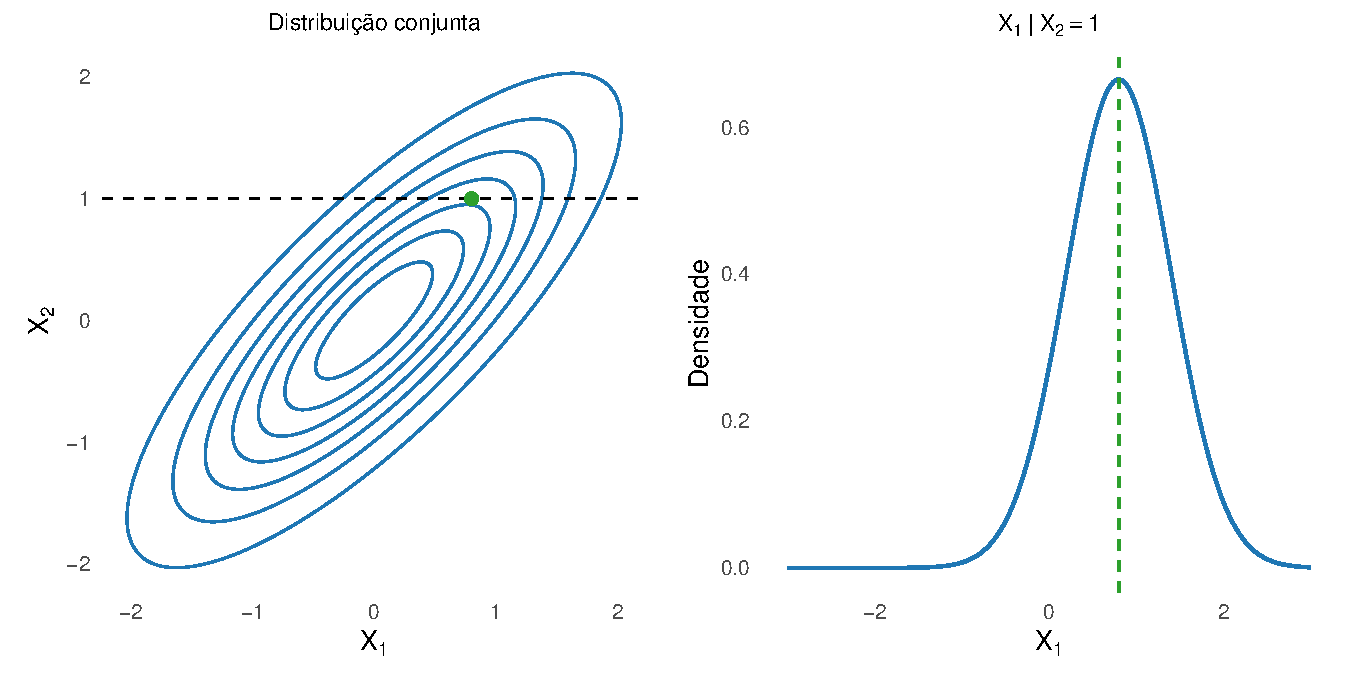
\includegraphics[keepaspectratio]{mod_2_normal_files/figure-pdf/fig-condicional-normal-1.pdf}}

}

\caption{\label{fig-condicional-normal}Distribuição normal bivariada e
densidade condicional de \(X_1\) para \(X_2=1\).}

\end{figure}%

No primeiro painel, a linha horizontal identifica o valor condicionado
\(X_2=1\). O ponto sobre essa linha indica a média da distribuição
condicional de \(X_1\).

O segundo painel mostra

\[
X_1
\mid
X_2=1
\sim
N
\left(
0,8,
0,36
\right).
\]

Em relação à distribuição marginal \(N(0,1)\), a média passa de \(0\)
para \(0,8\) e a variância passa de \(1\) para \(0,36\). O exemplo
ilustra duas propriedades gerais: a média condicional depende do valor
condicionado, enquanto a matriz de covariâncias condicional não depende
desse valor.

O branqueamento desenvolvido anteriormente permite agora obter uma
segunda consequência probabilística da normalidade: a distribuição exata
da distância quadrática de Mahalanobis.

\section{Distância de Mahalanobis e regiões de
probabilidade}\label{distuxe2ncia-de-mahalanobis-e-regiuxf5es-de-probabilidade}

O Capítulo 8 definiu em Definição~\ref{def-distancia-mahalanobis} a
distância de Mahalanobis como uma medida geométrica adaptada à estrutura
de covariâncias. Quando

\[
\boldsymbol{\mathsf X}
\sim
N_p
\left(
\boldsymbol{\mu},
\boldsymbol{\Sigma}
\right),
\qquad
\boldsymbol{\Sigma}
\succ
\mathbf0,
\]

a distância quadrática ao vetor de médias possui uma distribuição
probabilística conhecida.

Considere

\[
\boldsymbol{\mathsf X}
\sim
N_p
\left(
\boldsymbol{\mu},
\boldsymbol{\Sigma}
\right),
\]

com

\[
\boldsymbol{\Sigma}
\succ
\mathbf 0.
\]

A variável aleatória

\begin{equation}\phantomsection\label{eq-distancia-mahalanobis-aleatoria}{
D_M^2
=
\left(
\boldsymbol{\mathsf X}
-
\boldsymbol{\mu}
\right)^\top
\boldsymbol{\Sigma}^{-1}
\left(
\boldsymbol{\mathsf X}
-
\boldsymbol{\mu}
\right)
}\end{equation}

representa a distância quadrática de Mahalanobis entre uma realização
aleatória e o centro populacional.

\subsection{Distribuição
qui-quadrado}\label{distribuiuxe7uxe3o-qui-quadrado}

\begin{proposition}[Distribuição da distância quadrática de
Mahalanobis]\protect\hypertarget{prp-mahalanobis-qui-quadrado}{}\label{prp-mahalanobis-qui-quadrado}

A distância quadrática de Mahalanobis

\begin{equation}\phantomsection\label{eq-mahalanobis-distribuicao-qui-quadrado}{
D_M^2
=
\left(
\boldsymbol{\mathsf X}
-
\boldsymbol{\mu}
\right)^\top
\boldsymbol{\Sigma}^{-1}
\left(
\boldsymbol{\mathsf X}
-
\boldsymbol{\mu}
\right)
\sim
\chi_p^2,
}\end{equation}

para

\[
\boldsymbol{\mathsf X}
\sim
N_p
\left(
\boldsymbol{\mu},
\boldsymbol{\Sigma}
\right),
\qquad
\boldsymbol{\Sigma}
\succ
\mathbf0.
\]

\end{proposition}

\begin{proof}
Pelo branqueamento na Equação~\ref{eq-branqueamento-normal},

\[
\boldsymbol{\mathsf Z}
=
\boldsymbol{\Sigma}^{-1/2}
\left(
\boldsymbol{\mathsf X}
-
\boldsymbol{\mu}
\right)
\sim
N_p
\left(
\mathbf 0,
\mathbf I_p
\right).
\]

As componentes

\[
Z_1,\ldots,Z_p
\]

são, portanto, normais padrão independentes.

Além disso,

\[
\begin{aligned}
D_M^2
&=
\left(
\boldsymbol{\mathsf X}
-
\boldsymbol{\mu}
\right)^\top
\boldsymbol{\Sigma}^{-1}
\left(
\boldsymbol{\mathsf X}
-
\boldsymbol{\mu}
\right)\\
&=
\left[
\boldsymbol{\Sigma}^{-1/2}
\left(
\boldsymbol{\mathsf X}
-
\boldsymbol{\mu}
\right)
\right]^\top
\left[
\boldsymbol{\Sigma}^{-1/2}
\left(
\boldsymbol{\mathsf X}
-
\boldsymbol{\mu}
\right)
\right]\\
&=
\boldsymbol{\mathsf Z}^\top
\boldsymbol{\mathsf Z}\\
&=
\sum_{j=1}^{p}
Z_j^2.
\end{aligned}
\]

A soma dos quadrados de \(p\) variáveis normais padrão independentes
possui distribuição qui-quadrado com \(p\) graus de liberdade. Logo,

\[
D_M^2
\sim
\chi_p^2.
\]
\end{proof}

Como \(\boldsymbol{\Sigma}\succ\mathbf0\), a dimensão da distribuição é
\(p\), que determina os graus de liberdade da distribuição qui-quadrado.

Consequentemente,

\[
E
\left(
D_M^2
\right)
=
p
\]

e

\begin{equation}\phantomsection\label{eq-momentos-distancia-mahalanobis-normal}{
\operatorname{Var}
\left(
D_M^2
\right)
=
2p.
}\end{equation}

A escala de \(D_M^2\) depende, portanto, da dimensão. Sob o modelo
normal, seu valor esperado é \(p\), e não zero.

A igualdade

\[
E
\left(
D_M^2
\right)
=
p
\]

não depende da normalidade multivariada. No Capítulo 8,
Equação~\ref{eq-esperanca-mahalanobis-quadratica} obteve esse resultado
a partir apenas da estrutura de segunda ordem, para qualquer vetor
aleatório com vetor de médias \(\boldsymbol{\mu}\) e matriz de
covariâncias positiva definida \(\boldsymbol{\Sigma}\).

A hipótese de normalidade fornece um resultado mais forte:

\[
D_M^2
\sim
\chi_p^2.
\]

Assim, no presente capítulo, além do valor esperado, passa-se a conhecer
a distribuição completa da distância quadrática de Mahalanobis,
incluindo sua variância e seus quantis.

No espaço branqueado,

\[
D_M^2
=
\left\|
\boldsymbol{\mathsf Z}
\right\|^2.
\]

Assim, a distância quadrática de Mahalanobis no espaço original
corresponde ao quadrado da distância euclidiana à origem no espaço
branqueado.

\begin{tcolorbox}[enhanced jigsaw, colback=white, breakable, bottomrule=.15mm, left=2mm, arc=.35mm, rightrule=.15mm, colframe=quarto-callout-caution-color-frame, toprule=.15mm, leftrule=.75mm, opacityback=0]

\vspace{-3mm}\textbf{Parâmetros populacionais e quantidades estimadas}\vspace{3mm}

O resultado

\[
D_M^2
\sim
\chi_p^2
\]

utiliza os parâmetros populacionais \(\boldsymbol{\mu}\) e
\(\boldsymbol{\Sigma}\).

Se esses parâmetros forem substituídos por estimativas obtidas a partir
de uma amostra, a distribuição da forma quadrática resultante não será,
em geral, \(\chi_p^2\).

A distinção entre parâmetros populacionais e quantidades estimadas a
partir da amostra será desenvolvida nos Capítulos 10 e 12.

\end{tcolorbox}

\subsection{Regiões elipsoidais de
probabilidade}\label{regiuxf5es-elipsoidais-de-probabilidade}

\begin{definition}[Região elipsoidal de
probabilidade]\protect\hypertarget{def-regiao-concentracao-normal}{}\label{def-regiao-concentracao-normal}

Para

\[
\boldsymbol{\mathsf X}
\sim
N_p
\left(
\boldsymbol{\mu},
\boldsymbol{\Sigma}
\right),
\qquad
\boldsymbol{\Sigma}
\succ
\mathbf0,
\]

a \textbf{região elipsoidal de probabilidade \(1-\alpha\)} é

\begin{equation}\phantomsection\label{eq-regiao-concentracao-normal}{
\mathcal E_{1-\alpha}
=
\left\{
\mathbf x\in\mathbb{R}^p:
\left(
\mathbf x-\boldsymbol{\mu}
\right)^\top
\boldsymbol{\Sigma}^{-1}
\left(
\mathbf x-\boldsymbol{\mu}
\right)
\leq
\chi^2_{p;1-\alpha}
\right\},
}\end{equation}

em que \(0<\alpha<1\) e \(\chi^2_{p;1-\alpha}\) é o quantil de ordem
\(1-\alpha\) da distribuição \(\chi_p^2\).

Consequentemente,

\[
P
\left(
\boldsymbol{\mathsf X}
\in
\mathcal E_{1-\alpha}
\right)
=
1-\alpha.
\]

\end{definition}

Pela Proposição~\ref{prp-mahalanobis-qui-quadrado},

\begin{equation}\phantomsection\label{eq-probabilidade-regiao-concentracao-normal}{
\begin{aligned}
P
\left(
\boldsymbol{\mathsf X}
\in
\mathcal E_{1-\alpha}
\right)
&=
P
\left[
D_M^2
\leq
\chi^2_{p;1-\alpha}
\right]\\
&=
P
\left[
\chi_p^2
\leq
\chi^2_{p;1-\alpha}
\right]\\
&=
1-\alpha.
\end{aligned}
}\end{equation}

Portanto, \(\mathcal E_{1-\alpha}\) é uma região populacional que contém
uma realização de \(\boldsymbol{\mathsf X}\) com probabilidade
\(1-\alpha\).

Sua fronteira é

\[
\left(
\mathbf x-\boldsymbol{\mu}
\right)^\top
\boldsymbol{\Sigma}^{-1}
\left(
\mathbf x-\boldsymbol{\mu}
\right)
=
\chi^2_{p;1-\alpha}.
\]

A geometria é a mesma dos elipsoides de Mahalanobis definidos na
Equação~\ref{eq-elipsoide-covariancia} no Capítulo 8. A novidade do
modelo normal é a calibração probabilística da constante. Como naquele
capítulo o elipsoide foi definido por

\[
d_M^2
\left(
\mathbf x,
\boldsymbol{\mu}
\right)
\leq
c^2,
\]

a região de probabilidade \(1-\alpha\) é obtida fazendo

\[
c^2
=
\chi^2_{p;1-\alpha},
\]

ou, equivalentemente,

\[
c
=
\sqrt{
\chi^2_{p;1-\alpha}
}.
\]

No espaço branqueado, a região corresponde à esfera

\[
\left\{
\mathbf z\in\mathbb{R}^p:
\mathbf z^\top\mathbf z
\leq
\chi^2_{p;1-\alpha}
\right\},
\]

de raio

\[
\sqrt{
\chi^2_{p;1-\alpha}
}.
\]

As superfícies de igual densidade e as fronteiras das regiões
elipsoidais de probabilidade possuem a mesma forma geométrica porque
ambas são determinadas por valores constantes de \(d_M^2\). A diferença
está na escolha da constante: nas regiões de probabilidade, ela é
determinada por um quantil da distribuição \(\chi_p^2\).

\begin{tcolorbox}[enhanced jigsaw, colback=white, breakable, bottomrule=.15mm, left=2mm, arc=.35mm, rightrule=.15mm, colframe=quarto-callout-caution-color-frame, toprule=.15mm, leftrule=.75mm, opacityback=0]

\vspace{-3mm}\textbf{Região de probabilidade e região de confiança}\vspace{3mm}

A região

\[
\mathcal E_{1-\alpha}
\]

refere-se à posição de uma \textbf{realização de
\(\boldsymbol{\mathsf X}\)} quando os parâmetros populacionais
\(\boldsymbol{\mu}\) e \(\boldsymbol{\Sigma}\) são conhecidos.

Ela não é uma região de confiança para \(\boldsymbol{\mu}\).

Regiões de confiança para parâmetros populacionais serão construídas no
Capítulo 12 a partir de distribuições amostrais.

\end{tcolorbox}

\subsection{Avaliação de uma observação
fixa}\label{avaliauxe7uxe3o-de-uma-observauxe7uxe3o-fixa}

Considere agora um ponto fixo

\[
\mathbf x_0
\in
\mathbb{R}^p.
\]

Sua distância quadrática de Mahalanobis em relação ao modelo é

\begin{equation}\phantomsection\label{eq-mahalanobis-observacao-fixa}{
d_M^2
\left(
\mathbf x_0,
\boldsymbol{\mu}
\right)
=
\left(
\mathbf x_0-\boldsymbol{\mu}
\right)^\top
\boldsymbol{\Sigma}^{-1}
\left(
\mathbf x_0-\boldsymbol{\mu}
\right).
}\end{equation}

O ponto está dentro de \(\mathcal E_{1-\alpha}\) quando

\begin{equation}\phantomsection\label{eq-criterio-regiao-observacao-fixa}{
d_M^2
\left(
\mathbf x_0,
\boldsymbol{\mu}
\right)
\leq
\chi^2_{p;1-\alpha}.
}\end{equation}

Se

\[
d_M^2
\left(
\mathbf x_0,
\boldsymbol{\mu}
\right)
>
\chi^2_{p;1-\alpha},
\]

a observação está fora da região que contém probabilidade populacional
\(1-\alpha\).

Essa comparação descreve a posição de um valor já observado em relação
ao modelo. Depois que \(\mathbf x_0\) foi fixado, não se atribui a ele
probabilidade de pertencer à região: ele está dentro ou fora dela.

Também pode ser calculada a probabilidade de cauda

\begin{equation}\phantomsection\label{eq-probabilidade-cauda-mahalanobis}{
p_M
=
P
\left[
\chi_p^2
\geq
d_M^2
\left(
\mathbf x_0,
\boldsymbol{\mu}
\right)
\right].
}\end{equation}

A quantidade \(p_M\) mede, sob o modelo populacional completamente
especificado, a probabilidade de obter uma distância quadrática de
Mahalanobis pelo menos tão grande quanto a observada.

Um valor pequeno indica que \(\mathbf x_0\) se encontra em uma região de
afastamentos pouco frequentes sob a distribuição especificada. Essa
interpretação depende de \(\boldsymbol{\mu}\) e \(\boldsymbol{\Sigma}\)
serem parâmetros populacionais conhecidos e não constitui, neste ponto,
um procedimento inferencial para detecção de observações atípicas com
parâmetros estimados.

\begin{example}[Avaliação de uma observação em uma normal
bivariada]\protect\hypertarget{exm-regiao-concentracao-normal}{}\label{exm-regiao-concentracao-normal}

Considere

\[
\boldsymbol{\mathsf X}
\sim
N_2
\left(
\begin{bmatrix}
0\\
0
\end{bmatrix},
\begin{bmatrix}
4 & 1\\
1 & 1
\end{bmatrix}
\right)
\]

e

\[
\mathbf x_0
=
\begin{bmatrix}
3\\
1
\end{bmatrix}.
\]

A inversa da matriz de covariâncias é

\[
\boldsymbol{\Sigma}^{-1}
=
\frac{1}{3}
\begin{bmatrix}
1 & -1\\
-1 & 4
\end{bmatrix}.
\]

Logo,

\[
\begin{aligned}
d_M^2
\left(
\mathbf x_0,
\boldsymbol{\mu}
\right)
&=
\begin{bmatrix}
3 & 1
\end{bmatrix}
\frac{1}{3}
\begin{bmatrix}
1 & -1\\
-1 & 4
\end{bmatrix}
\begin{bmatrix}
3\\
1
\end{bmatrix}\\
&=
\frac{7}{3}\\
&\approx
2,33.
\end{aligned}
\]

Para a região que contém probabilidade \(0,95\),

\[
\chi^2_{2;0,95}
\approx
5,99.
\]

Como

\[
2,33
<
5,99,
\]

a observação está dentro da região elipsoidal que contém \(95\%\) da
probabilidade populacional.

A probabilidade de cauda associada à distância observada é

\[
\begin{aligned}
p_M
&=
P
\left(
\chi_2^2
\geq
2,33
\right)\\
&\approx
0,31.
\end{aligned}
\]

Assim, aproximadamente \(31\%\) dos vetores gerados pelo modelo
apresentam distância quadrática de Mahalanobis ao centro pelo menos tão
grande quanto a observada. O ponto, portanto, não apresenta um
afastamento particularmente extremo em relação à distribuição
especificada.

\end{example}

O exemplo utiliza parâmetros populacionais conhecidos. Se o vetor de
médias e a matriz de covariâncias fossem substituídos por estimativas
amostrais, seria necessário utilizar a teoria inferencial apropriada.

Os resultados desta seção mostram a passagem da geometria da distância
de Mahalanobis e de seus elipsoides, desenvolvida em
Definição~\ref{def-distancia-mahalanobis} e
Equação~\ref{eq-elipsoide-covariancia}, para uma interpretação
probabilística. Sob normalidade multivariada e
\(\boldsymbol{\Sigma}\succ\mathbf0\), a forma quadrática de Mahalanobis
possui distribuição \(\chi_p^2\), permitindo calibrar os elipsoides por
probabilidades populacionais.

A comparação entre duas distribuições normais permite observar, em
seguida, como mudanças no vetor de médias e na matriz de covariâncias
modificam suas posições, formas e densidades. Essa comparação será
utilizada somente como motivação para técnicas de discriminação
desenvolvidas posteriormente.

\section{Comparação entre distribuições
normais}\label{comparauxe7uxe3o-entre-distribuiuxe7uxf5es-normais}

Considere duas populações descritas por distribuições normais
multivariadas:

\[
\boldsymbol{\mathsf X}_{1}
\sim
N_p
\left(
\boldsymbol{\mu}_1,
\boldsymbol{\Sigma}_1
\right)
\]

e

\[
\boldsymbol{\mathsf X}_{2}
\sim
N_p
\left(
\boldsymbol{\mu}_2,
\boldsymbol{\Sigma}_2
\right),
\]

com

\[
\boldsymbol{\Sigma}_1
\succ
\mathbf 0
\qquad
\text{e}
\qquad
\boldsymbol{\Sigma}_2
\succ
\mathbf 0.
\]

Os vetores de médias determinam a localização das distribuições,
enquanto as matrizes de covariâncias determinam sua dispersão,
orientação e forma. A comparação entre duas distribuições normais
permite observar como esses dois componentes da parametrização atuam
conjuntamente.

\subsection{Médias distintas e covariância
comum}\label{muxe9dias-distintas-e-covariuxe2ncia-comum}

Suponha

\[
\boldsymbol{\Sigma}_1
=
\boldsymbol{\Sigma}_2
=
\boldsymbol{\Sigma},
\]

mas

\[
\boldsymbol{\mu}_1
\neq
\boldsymbol{\mu}_2.
\]

As duas distribuições possuem superfícies de igual densidade com a mesma
forma, orientação e extensão, mas centradas em pontos diferentes.

Pela log-densidade na
Equação~\ref{eq-log-densidade-normal-multivariada}, ambas contêm o termo
quadrático

\[
-\frac12
\mathbf x^\top
\boldsymbol{\Sigma}^{-1}
\mathbf x.
\]

Ao comparar as duas log-densidades, esse termo é comum e se cancela. De
fato,

\begin{equation}\phantomsection\label{eq-log-razao-normal-covariancia-comum}{
\begin{aligned}
\log
\frac{
f_1(\mathbf x)
}{
f_2(\mathbf x)
}
&=
\mathbf x^\top
\boldsymbol{\Sigma}^{-1}
\left(
\boldsymbol{\mu}_1
-
\boldsymbol{\mu}_2
\right)
\\
&\quad
-
\frac12
\left(
\boldsymbol{\mu}_1^\top
\boldsymbol{\Sigma}^{-1}
\boldsymbol{\mu}_1
-
\boldsymbol{\mu}_2^\top
\boldsymbol{\Sigma}^{-1}
\boldsymbol{\mu}_2
\right).
\end{aligned}
}\end{equation}

A log-razão entre as densidades é, portanto, uma função afim de
\(\mathbf x\).

Consequentemente, o conjunto

\[
\left\{
\mathbf x\in\mathbb{R}^p:
f_1(\mathbf x)
=
f_2(\mathbf x)
\right\}
\]

é um hiperplano.

A matriz de covariâncias comum influencia a orientação desse hiperplano
por meio do vetor

\[
\boldsymbol{\Sigma}^{-1}
\left(
\boldsymbol{\mu}_1
-
\boldsymbol{\mu}_2
\right),
\]

que determina sua direção normal. Assim, a separação entre os centros é
avaliada segundo a geometria induzida pela matriz de covariâncias comum.

\subsection{Covariâncias distintas}\label{covariuxe2ncias-distintas}

Considere agora

\[
\boldsymbol{\Sigma}_1
\neq
\boldsymbol{\Sigma}_2.
\]

As distribuições podem diferir não somente quanto à localização, mas
também quanto à forma, orientação e extensão de suas superfícies de
igual densidade.

Nesse caso, as log-densidades envolvem as formas quadráticas

\[
-\frac12
\left(
\mathbf x-\boldsymbol{\mu}_1
\right)^\top
\boldsymbol{\Sigma}_1^{-1}
\left(
\mathbf x-\boldsymbol{\mu}_1
\right)
\]

e

\[
-\frac12
\left(
\mathbf x-\boldsymbol{\mu}_2
\right)^\top
\boldsymbol{\Sigma}_2^{-1}
\left(
\mathbf x-\boldsymbol{\mu}_2
\right).
\]

Como as matrizes inversas são diferentes, os termos quadráticos em
\(\mathbf x\) não se cancelam em geral. Expandindo a diferença entre as
log-densidades,

\begin{equation}\phantomsection\label{eq-log-razao-normal-covariancias-distintas}{
\begin{aligned}
\log
\frac{
f_1(\mathbf x)
}{
f_2(\mathbf x)
}
&=
-\frac12
\mathbf x^\top
\left(
\boldsymbol{\Sigma}_1^{-1}
-
\boldsymbol{\Sigma}_2^{-1}
\right)
\mathbf x
\\
&\quad
+
\mathbf x^\top
\left(
\boldsymbol{\Sigma}_1^{-1}
\boldsymbol{\mu}_1
-
\boldsymbol{\Sigma}_2^{-1}
\boldsymbol{\mu}_2
\right)
\\
&\quad
-
\frac12
\left(
\boldsymbol{\mu}_1^\top
\boldsymbol{\Sigma}_1^{-1}
\boldsymbol{\mu}_1
-
\boldsymbol{\mu}_2^\top
\boldsymbol{\Sigma}_2^{-1}
\boldsymbol{\mu}_2
\right)
\\
&\quad
-
\frac12
\log
\left(
\frac{
|\boldsymbol{\Sigma}_1|
}{
|\boldsymbol{\Sigma}_2|
}
\right).
\end{aligned}
}\end{equation}

A presença do termo

\[
\mathbf x^\top
\left(
\boldsymbol{\Sigma}_1^{-1}
-
\boldsymbol{\Sigma}_2^{-1}
\right)
\mathbf x
\]

faz com que a log-razão seja, em geral, uma função quadrática de
\(\mathbf x\).

Assim, o conjunto de pontos nos quais

\[
f_1(\mathbf x)
=
f_2(\mathbf x)
\]

é determinado, em geral, por uma equação quadrática em \(\mathbf x\).
Sua geometria pode, portanto, diferir substancialmente do hiperplano
obtido no caso de covariância comum.

A Figura~\ref{fig-comparacao-distribuicoes-normais} ilustra as duas
situações.

\begin{figure}

\centering{

\pandocbounded{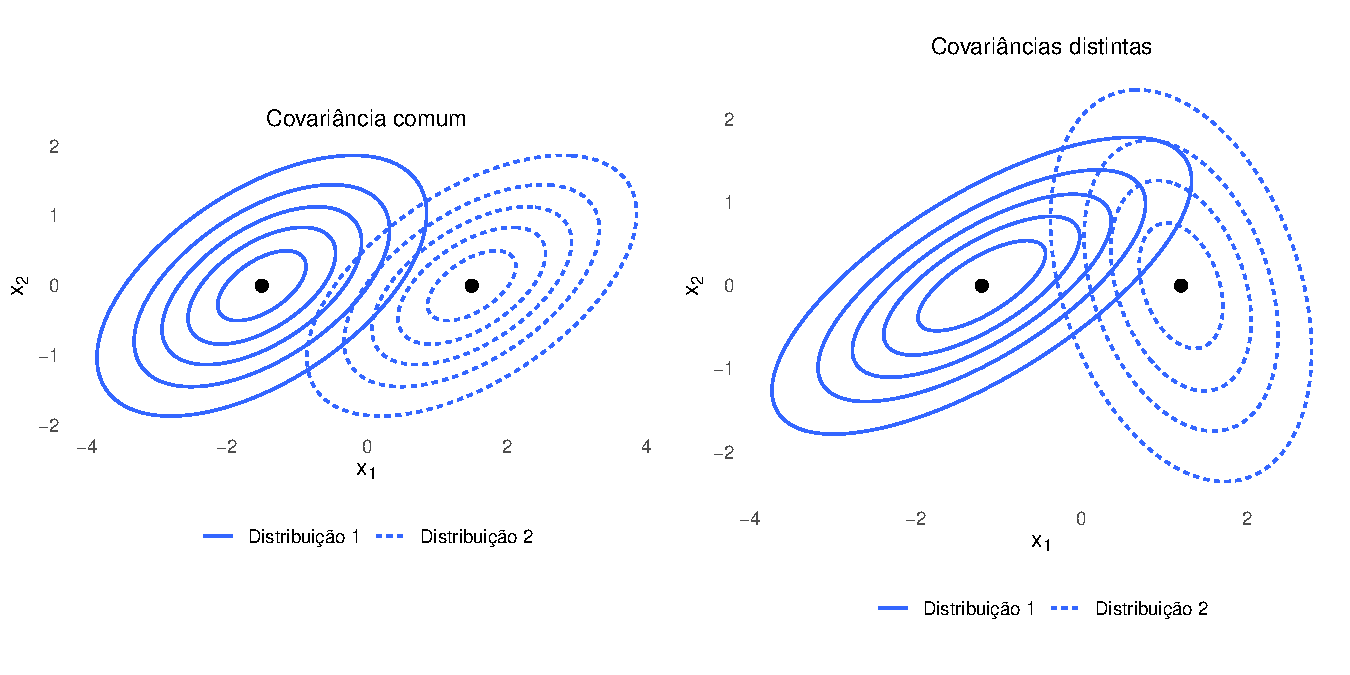
\includegraphics[keepaspectratio]{mod_2_normal_files/figure-pdf/fig-comparacao-distribuicoes-normais-1.pdf}}

}

\caption{\label{fig-comparacao-distribuicoes-normais}Comparação entre
distribuições normais bivariadas com covariância comum e com
covariâncias distintas.}

\end{figure}%

No primeiro painel, as duas distribuições apresentam superfícies de
nível com a mesma forma e orientação, deslocadas para centros
diferentes. No segundo, as diferenças entre as matrizes de covariâncias
modificam também a extensão e a orientação dessas superfícies.

A comparação mostra duas estruturas algébricas que serão utilizadas
posteriormente. Com uma matriz de covariâncias comum, a comparação das
log-densidades elimina os termos quadráticos comuns e produz uma
expressão afim. Com matrizes de covariâncias distintas, permanecem, em
geral, termos quadráticos.

Esses resultados serão retomados na formulação da Análise Discriminante.
A construção de regras de classificação, probabilidades a priori, custos
de decisão e estimação dos parâmetros pertence aos módulos posteriores.

\section{Alcance da hipótese de
normalidade}\label{alcance-da-hipuxf3tese-de-normalidade}

A distribuição normal multivariada acrescenta uma estrutura
probabilística específica aos objetos desenvolvidos nos capítulos
anteriores. É importante distinguir quais resultados dependem dessa
hipótese e quais permanecem válidos para vetores aleatórios mais gerais.

\subsection{Resultados que não exigem
normalidade}\label{resultados-que-nuxe3o-exigem-normalidade}

Diversos resultados utilizados neste capítulo dependem somente da
existência dos momentos necessários.

Para um vetor aleatório com média \(\boldsymbol{\mu}\) e matriz de
covariâncias \(\boldsymbol{\Sigma}\),

\[
E
\left(
\mathbf a^\top
\boldsymbol{\mathsf X}
\right)
=
\mathbf a^\top
\boldsymbol{\mu}
\]

e

\[
\operatorname{Var}
\left(
\mathbf a^\top
\boldsymbol{\mathsf X}
\right)
=
\mathbf a^\top
\boldsymbol{\Sigma}
\mathbf a
\]

não exigem normalidade.

Da mesma forma, para

\[
\boldsymbol{\mathsf Y}
=
\mathbf A
\boldsymbol{\mathsf X}
+
\mathbf b,
\]

as relações

\[
E
\left(
\boldsymbol{\mathsf Y}
\right)
=
\mathbf A
\boldsymbol{\mu}
+
\mathbf b
\]

e

\[
\operatorname{Cov}
\left(
\boldsymbol{\mathsf Y}
\right)
=
\mathbf A
\boldsymbol{\Sigma}
\mathbf A^\top
\]

são propriedades gerais dos primeiros e segundos momentos.

A matriz de covariâncias continua simétrica e positiva semidefinida,
conforme Proposição~\ref{prp-estrutura-matriz-covariancias}; a distância
de Mahalanobis continua definindo a geometria apresentada na
Definição~\ref{def-distancia-mahalanobis} quando a matriz de
covariâncias é positiva definida; e o complemento de Schur continua
representando a covariância do resíduo do melhor ajuste linear entre
blocos, conforme
Proposição~\ref{prp-complemento-schur-covariancia-residual}. Esses
resultados foram desenvolvidos no Capítulo 8 sem hipótese de
normalidade.

Também não depende da normalidade a esperança de uma forma quadrática
centrada. Para uma matriz simétrica \(\mathbf A\),

\[
E
\left[
\left(
\boldsymbol{\mathsf X}
-
\mathbf a
\right)^\top
\mathbf A
\left(
\boldsymbol{\mathsf X}
-
\mathbf a
\right)
\right]
=
\operatorname{tr}
\left(
\mathbf A
\boldsymbol{\Sigma}
\right)
+
\left(
\boldsymbol{\mu}
-
\mathbf a
\right)^\top
\mathbf A
\left(
\boldsymbol{\mu}
-
\mathbf a
\right),
\]

desde que existam os momentos de segunda ordem necessários.

Em particular, quando \(\boldsymbol{\Sigma}\succ\mathbf0\),

\[
E
\left[
\left(
\boldsymbol{\mathsf X}
-
\boldsymbol{\mu}
\right)^\top
\boldsymbol{\Sigma}^{-1}
\left(
\boldsymbol{\mathsf X}
-
\boldsymbol{\mu}
\right)
\right]
=
p.
\]

Portanto, o valor esperado da distância quadrática de Mahalanobis é uma
propriedade de segunda ordem e não uma consequência específica da
normalidade.

Esses resultados descrevem estruturas de primeira e segunda ordem. Eles
não determinam, por si mesmos, a distribuição conjunta.

\subsection{Resultados específicos da família
normal}\label{resultados-especuxedficos-da-famuxedlia-normal}

A hipótese de normalidade conjunta produz propriedades adicionais.

Entre os resultados desenvolvidos neste capítulo estão:

\begin{itemize}
\tightlist
\item
  o vetor de médias e a matriz de covariâncias determinam completamente
  a distribuição;
\item
  transformações afins preservam a família normal;
\item
  distribuições marginais de subvectores permanecem normais;
\item
  covariância cruzada nula entre blocos conjuntamente normais equivale à
  independência;
\item
  distribuições condicionais permanecem normais;
\item
  a esperança condicional entre blocos é uma função afim do bloco
  condicionante;
\item
  a matriz de covariâncias condicional é o complemento de Schur
  correspondente;
\item
  quando \(\boldsymbol{\Sigma}\succ\mathbf0\), o branqueamento produz
  componentes normais padrão independentes;
\item
  quando \(\boldsymbol{\Sigma}\succ\mathbf0\), a distância quadrática de
  Mahalanobis populacional possui distribuição \(\chi_p^2\).
\end{itemize}

A equivalência

\[
\boldsymbol{\Sigma}_{12}
=
\mathbf 0
\quad
\Longleftrightarrow
\quad
\boldsymbol{\mathsf X}_1
\perp
\boldsymbol{\mathsf X}_2
\]

é um exemplo da diferença entre uma propriedade geral de covariância e
uma propriedade específica da família normal.

A implicação

\[
\boldsymbol{\mathsf X}_1
\perp
\boldsymbol{\mathsf X}_2
\quad
\Longrightarrow
\quad
\boldsymbol{\Sigma}_{12}
=
\mathbf 0
\]

vale, quando os segundos momentos existem, sem normalidade. A implicação
inversa requer a estrutura normal conjunta estabelecida na
Proposição~\ref{prp-independencia-blocos-normais}.

De maneira semelhante, a igualdade

\[
E
\left(
D_M^2
\right)
=
p
\]

decorre apenas da estrutura de segunda ordem, mas a afirmação

\[
D_M^2
=
\left(
\boldsymbol{\mathsf X}
-
\boldsymbol{\mu}
\right)^\top
\boldsymbol{\Sigma}^{-1}
\left(
\boldsymbol{\mathsf X}
-
\boldsymbol{\mu}
\right)
\sim
\chi_p^2
\]

é específica do modelo normal multivariado sob
\(\boldsymbol{\Sigma}\succ\mathbf0\).

Assim, conhecer apenas \(\boldsymbol{\mu}\) e \(\boldsymbol{\Sigma}\)
permite determinar a esperança dessa forma quadrática, mas não sua
distribuição completa. A distribuição qui-quadrado estabelecida na
Proposição~\ref{prp-mahalanobis-qui-quadrado} depende da normalidade
multivariada.

Assim, a normalidade transforma relações entre médias, covariâncias e
formas quadráticas em afirmações sobre distribuições completas.

\subsection{Passagem do modelo populacional para a
inferência}\label{passagem-do-modelo-populacional-para-a-inferuxeancia}

Neste capítulo, \(\boldsymbol{\mu}\) e \(\boldsymbol{\Sigma}\) foram
tratados como parâmetros populacionais que caracterizam a distribuição,
sem abordar sua estimação a partir de uma amostra. Essa escolha permitiu
estudar diretamente as propriedades da distribuição

\[
N_p
\left(
\boldsymbol{\mu},
\boldsymbol{\Sigma}
\right).
\]

Em uma aplicação estatística, esses parâmetros são geralmente
desconhecidos. A observação de uma amostra introduz uma nova distinção
entre:

\begin{itemize}
\tightlist
\item
  parâmetros populacionais;
\item
  estatísticas aleatórias;
\item
  estimadores;
\item
  valores calculados a partir dos dados observados.
\end{itemize}

Essa distinção modifica alguns resultados. Por exemplo,

\[
\left(
\boldsymbol{\mathsf X}
-
\boldsymbol{\mu}
\right)^\top
\boldsymbol{\Sigma}^{-1}
\left(
\boldsymbol{\mathsf X}
-
\boldsymbol{\mu}
\right)
\sim
\chi_p^2
\]

não autoriza substituir diretamente \(\boldsymbol{\mu}\) e
\(\boldsymbol{\Sigma}\) por estimativas e manter a mesma distribuição.

Da mesma forma, conhecer a forma da densidade normal não é suficiente
para realizar inferência sobre parâmetros desconhecidos. É necessário
especificar uma amostra aleatória, construir estatísticas e estudar suas
propriedades e distribuições amostrais.

O Capítulo 10 inicia essa passagem. O modelo probabilístico permanece o
ponto de partida, mas os parâmetros populacionais passam a ser
relacionados a estatísticas e estimadores construídos a partir da
amostra.

\section{Aprofundamento: Normal Singular}\label{sec-normal-singular}

\begin{tcolorbox}[enhanced jigsaw, colback=white, breakable, bottomrule=.15mm, left=2mm, arc=.35mm, rightrule=.15mm, colframe=quarto-callout-note-color-frame, toprule=.15mm, leftrule=.75mm, opacityback=0]

\vspace{-3mm}\textbf{Leitura de aprofundamento}\vspace{3mm}

A sequência principal do capítulo considerou

\[
\boldsymbol{\Sigma}
\succ
\mathbf0,
\]

de modo que a matriz de covariâncias é invertível e a distribuição
possui densidade em todo \(\mathbb R^p\).

Quando \(\boldsymbol{\Sigma}\) é positiva semidefinida, mas não positiva
definida, a distribuição normal multivariada é singular. Nesse caso,
parte das direções apresenta variância zero e a variabilidade fica
restrita a um subespaço de dimensão inferior a \(p\).

Esta seção reúne a definição, a representação em dimensão reduzida, o
suporte, a densidade no suporte, o branqueamento e a forma generalizada
de Mahalanobis no caso singular.

\end{tcolorbox}

\begin{definition}[Distribuição normal multivariada
singular]\protect\hypertarget{def-normal-multivariada-singular}{}\label{def-normal-multivariada-singular}

Uma distribuição

\[
N_p
\left(
\boldsymbol{\mu},
\boldsymbol{\Sigma}
\right)
\]

é denominada \textbf{singular} ou \textbf{degenerada} quando

\[
\operatorname{posto}
\left(
\boldsymbol{\Sigma}
\right)
=
r
<
p.
\]

Como toda matriz de covariâncias é positiva semidefinida, esse caso
equivale a

\[
\boldsymbol{\Sigma}
\succeq
\mathbf0
\qquad
\text{e}
\qquad
\boldsymbol{\Sigma}
\not\succ
\mathbf0.
\]

A distribuição é \textbf{não singular} quando

\[
\operatorname{posto}
\left(
\boldsymbol{\Sigma}
\right)
=
p,
\]

equivalentemente,

\[
\boldsymbol{\Sigma}
\succ
\mathbf0.
\]

\end{definition}

A normal singular surge quando existem relações lineares exatas entre as
componentes do vetor. Se, por exemplo,

\[
X_3
=
X_1
+
X_2
\]

quase certamente, uma das componentes não acrescenta uma nova direção de
variabilidade e a matriz de covariâncias não possui posto completo.

O caso singular também pode resultar de uma transformação linear que
reduz a dimensão. Se

\[
\boldsymbol{\mathsf Y}
=
\mathbf A
\boldsymbol{\mathsf X}
+
\mathbf b
\in
\mathbb R^m
\]

e

\[
\operatorname{posto}
\left(
\mathbf A
\right)
<
m,
\]

então

\[
\operatorname{posto}
\left(
\mathbf A
\boldsymbol{\Sigma}
\mathbf A^\top
\right)
\leq
\operatorname{posto}
\left(
\mathbf A
\right)
<
m.
\]

Portanto,

\[
\operatorname{Cov}
\left(
\boldsymbol{\mathsf Y}
\right)
=
\mathbf A
\boldsymbol{\Sigma}
\mathbf A^\top
\]

é singular.

A distribuição normal singular fornece, portanto, um modelo
probabilístico para vetores normais sujeitos a restrições lineares
exatas ou representados em um espaço ambiente de dimensão maior que sua
dimensão probabilística efetiva.

A singularidade de uma matriz de covariâncias amostral, entretanto, não
implica que a matriz de covariâncias populacional seja singular. Como
será formalizado em Equação~\ref{eq-posto-sscp-amostral}, quando
\(p\geq n\), a matriz de covariâncias amostral possui posto no máximo
\(n-1\) e é necessariamente singular, mesmo que a matriz populacional
seja positiva definida.

Nos desenvolvimentos a seguir, considere

\[
1
\leq
r
=
\operatorname{posto}
\left(
\boldsymbol{\Sigma}
\right)
<
p.
\]

O caso extremo \(r=0\) será apresentado ao final da seção.

Como \(\boldsymbol{\Sigma}\) é simétrica e positiva semidefinida,
Teorema~\ref{thm-teorema-espectral} e
Proposição~\ref{prp-positividade-autovalores} garantem que sua
decomposição espectral reduzida pode ser escrita como

\begin{equation}\phantomsection\label{eq-decomposicao-espectral-normal-singular}{
\boldsymbol{\Sigma}
=
\mathbf Q_r
\boldsymbol{\Lambda}_r
\mathbf Q_r^\top.
}\end{equation}

em que

\[
\mathbf Q_r
\in
\mathbb{R}^{p\times r}
\]

possui colunas ortonormais associadas aos \(r\) autovalores positivos e

\[
\boldsymbol{\Lambda}_r
=
\operatorname{diag}
\left(
\lambda_1,\ldots,\lambda_r
\right),
\qquad
\lambda_j>0.
\]

Por Proposição~\ref{prp-nucleo-imagem-espectral},

\[
\mathcal C
\left(
\boldsymbol{\Sigma}
\right)
=
\mathcal C
\left(
\mathbf Q_r
\right).
\]

Definindo

\[
\mathbf A_r
=
\mathbf Q_r
\boldsymbol{\Lambda}_r^{1/2},
\]

tem-se

\[
\boldsymbol{\Sigma}
=
\mathbf A_r
\mathbf A_r^\top.
\]

Logo, uma representação da distribuição singular é

\begin{equation}\phantomsection\label{eq-representacao-normal-singular}{
\boldsymbol{\mathsf X}
\overset{d}{=}
\boldsymbol{\mu}
+
\mathbf A_r
\boldsymbol{\mathsf Z},
\qquad
\boldsymbol{\mathsf Z}
\sim
N_r
\left(
\mathbf 0,
\mathbf I_r
\right).
}\end{equation}

Por Proposição~\ref{prp-singularidade-matriz-covariancias}, a
singularidade de \(\boldsymbol{\Sigma}\) implica, para qualquer vetor
aleatório com essa matriz de covariâncias,

\[
\boldsymbol{\mathsf X}
-
\boldsymbol{\mu}
\in
\mathcal C
\left(
\boldsymbol{\Sigma}
\right)
\]

quase certamente. Na família normal, a representação na
Equação~\ref{eq-representacao-normal-singular} permite uma conclusão
mais forte: o subespaço afim

\[
\boldsymbol{\mu}
+
\mathcal C
\left(
\boldsymbol{\Sigma}
\right)
\]

constitui o suporte da distribuição.

\begin{proposition}[Suporte efetivo da normal
singular]\protect\hypertarget{prp-suporte-normal-singular}{}\label{prp-suporte-normal-singular}

Se

\[
\boldsymbol{\mathsf X}
\sim
N_p
\left(
\boldsymbol{\mu},
\boldsymbol{\Sigma}
\right)
\]

e

\[
\operatorname{posto}
\left(
\boldsymbol{\Sigma}
\right)
=
r
<
p,
\]

o suporte da distribuição é o subespaço afim

\[
\boldsymbol{\mu}
+
\mathcal C
\left(
\boldsymbol{\Sigma}
\right),
\]

de dimensão \(r\).

Consequentemente,

\begin{equation}\phantomsection\label{eq-suporte-normal-singular}{
P
\left[
\boldsymbol{\mathsf X}
\in
\boldsymbol{\mu}
+
\mathcal C
\left(
\boldsymbol{\Sigma}
\right)
\right]
=
1.
}\end{equation}

\end{proposition}

\begin{proof}
Pela representação Equação~\ref{eq-representacao-normal-singular},

\[
\boldsymbol{\mathsf X}
\overset{d}{=}
\boldsymbol{\mu}
+
\mathbf A_r
\boldsymbol{\mathsf Z}.
\]

Como \(\boldsymbol{\Lambda}_r^{1/2}\) é invertível,

\[
\mathcal C
\left(
\mathbf A_r
\right)
=
\mathcal C
\left(
\mathbf Q_r
\right)
=
\mathcal C
\left(
\boldsymbol{\Sigma}
\right).
\]

Portanto,

\[
\mathbf A_r
\boldsymbol{\mathsf Z}
\in
\mathcal C
\left(
\boldsymbol{\Sigma}
\right)
\]

quase certamente, o que fornece
Equação~\ref{eq-suporte-normal-singular}.

Além disso, \(\mathbf A_r\) possui posto coluna \(r\). A aplicação

\[
\mathbf z
\longmapsto
\boldsymbol{\mu}
+
\mathbf A_r\mathbf z
\]

é uma transformação afim bijetiva entre \(\mathbb{R}^r\) e

\[
\boldsymbol{\mu}
+
\mathcal C
\left(
\boldsymbol{\Sigma}
\right).
\]

Como a normal padrão em \(\mathbb{R}^r\) possui densidade positiva em
todo \(\mathbb{R}^r\), todo conjunto relativamente aberto e não vazio
desse subespaço afim possui probabilidade positiva. Assim, esse
subespaço é o suporte da distribuição.
\end{proof}

A mesma estrutura pode ser caracterizada pelo núcleo da matriz de
covariâncias. Se

\[
\mathbf a
\in
\mathcal N
\left(
\boldsymbol{\Sigma}
\right),
\]

então

\[
\operatorname{Var}
\left[
\mathbf a^\top
\left(
\boldsymbol{\mathsf X}
-
\boldsymbol{\mu}
\right)
\right]
=
\mathbf a^\top
\boldsymbol{\Sigma}
\mathbf a
=
0,
\]

e, consequentemente,

\[
\mathbf a^\top
\left(
\boldsymbol{\mathsf X}
-
\boldsymbol{\mu}
\right)
=
0
\]

quase certamente.

As direções do núcleo são, portanto, direções sem variabilidade
probabilística.

A normal singular não possui densidade em relação à medida de Lebesgue
de dimensão \(p\) em \(\mathbb R^p\), pois toda a probabilidade está
concentrada no suporte

\[
\boldsymbol{\mu}
+
\mathcal C
\left(
\boldsymbol{\Sigma}
\right),
\]

de dimensão \(r<p\). Nesse suporte, entretanto, a distribuição possui
densidade relativamente à medida de volume \(r\)-dimensional, como será
mostrado a seguir.

\begin{example}[Normal bivariada concentrada em uma
reta]\protect\hypertarget{exm-normal-singular-reta}{}\label{exm-normal-singular-reta}

Considere

\[
Z
\sim
N(0,1)
\]

e defina

\[
\boldsymbol{\mathsf X}
=
\begin{bmatrix}
X_1\\
X_2
\end{bmatrix}
=
\begin{bmatrix}
Z\\
2Z
\end{bmatrix}.
\]

Equivalentemente,

\[
\boldsymbol{\mathsf X}
=
\begin{bmatrix}
1\\
2
\end{bmatrix}
Z.
\]

Logo,

\[
\boldsymbol{\mathsf X}
\sim
N_2
\left(
\begin{bmatrix}
0\\
0
\end{bmatrix},
\begin{bmatrix}
1 & 2\\
2 & 4
\end{bmatrix}
\right).
\]

A matriz de covariâncias possui posto 1 e

\[
X_2
=
2X_1
\]

quase certamente. Portanto, toda a distribuição está concentrada na reta

\[
x_2
=
2x_1.
\]

Embora o vetor tenha duas componentes, sua dimensão probabilística
efetiva é 1.

\end{example}

\begin{tcolorbox}[enhanced jigsaw, colback=white, breakable, bottomrule=.15mm, left=2mm, arc=.35mm, rightrule=.15mm, colframe=quarto-callout-note-color-frame, toprule=.15mm, leftrule=.75mm, opacityback=0]

\vspace{-3mm}\textbf{Densidade no suporte da normal singular}\vspace{3mm}

Por Proposição~\ref{prp-suporte-normal-singular}, a distribuição está
concentrada no subespaço afim

\[
\boldsymbol{\mu}
+
\mathcal C
\left(
\boldsymbol{\Sigma}
\right),
\]

de dimensão

\[
r
=
\operatorname{posto}
\left(
\boldsymbol{\Sigma}
\right).
\]

Retomando Equação~\ref{eq-decomposicao-espectral-normal-singular},

\[
\boldsymbol{\Sigma}
=
\mathbf Q_r
\boldsymbol{\Lambda}_r
\mathbf Q_r^\top,
\qquad
\boldsymbol{\Lambda}_r
=
\operatorname{diag}
\left(
\lambda_1,\ldots,\lambda_r
\right),
\]

a Definição~\ref{def-pseudoinversa-espectral} fornece

\[
\boldsymbol{\Sigma}^{+}
=
\mathbf Q_r
\boldsymbol{\Lambda}_r^{-1}
\mathbf Q_r^\top.
\]

Como

\[
\det
\left(
\boldsymbol{\Lambda}_r
\right)
=
\prod_{j=1}^{r}
\lambda_j
>
0,
\]

a densidade relativamente à medida de volume \(r\)-dimensional no
suporte afim pode ser escrita como

\begin{equation}\phantomsection\label{eq-densidade-normal-singular}{
f_{\mathrm{sup}}
\left(
\mathbf x
\right)
=
\frac{
1
}{
(2\pi)^{r/2}
\det
\left(
\boldsymbol{\Lambda}_r
\right)^{1/2}
}
\exp
\left[
-\frac12
\left(
\mathbf x-\boldsymbol{\mu}
\right)^\top
\boldsymbol{\Sigma}^{+}
\left(
\mathbf x-\boldsymbol{\mu}
\right)
\right],
}\end{equation}

para

\[
\mathbf x
\in
\boldsymbol{\mu}
+
\mathcal C
\left(
\boldsymbol{\Sigma}
\right).
\]

Essa expressão utiliza a mesma estrutura de
Equação~\ref{eq-densidade-normal-multivariada}, mas somente nas \(r\)
direções em que existe variabilidade (Anderson, 2003; Rao, 1973).

A conexão com uma normal não singular de dimensão \(r\) decorre
diretamente de Equação~\ref{eq-representacao-normal-singular}. Defina

\[
\boldsymbol{\mathsf Y}
=
\boldsymbol{\Lambda}_r^{1/2}
\boldsymbol{\mathsf Z},
\qquad
\boldsymbol{\mathsf Z}
\sim
N_r
\left(
\mathbf0,
\mathbf I_r
\right).
\]

Por Proposição~\ref{prp-construcao-afim-normal},

\[
\boldsymbol{\mathsf Y}
\sim
N_r
\left(
\mathbf0,
\boldsymbol{\Lambda}_r
\right).
\]

Assim, Equação~\ref{eq-representacao-normal-singular} pode ser escrita
como

\begin{equation}\phantomsection\label{eq-normal-singular-coordenadas-efetivas}{
\boldsymbol{\mathsf X}
\overset{d}{=}
\boldsymbol{\mu}
+
\mathbf Q_r
\boldsymbol{\mathsf Y}.
}\end{equation}

Portanto, a normal singular em \(\mathbb R^p\) corresponde à
representação de uma normal não singular de dimensão \(r\) no subespaço
afim

\[
\boldsymbol{\mu}
+
\mathcal C
\left(
\boldsymbol{\Sigma}
\right).
\]

\end{tcolorbox}

\begin{tcolorbox}[enhanced jigsaw, colback=white, breakable, bottomrule=.15mm, left=2mm, arc=.35mm, rightrule=.15mm, colframe=quarto-callout-note-color-frame, toprule=.15mm, leftrule=.75mm, opacityback=0]

\vspace{-3mm}\textbf{Branqueamento no caso singular}\vspace{3mm}

Se

\[
\operatorname{posto}
\left(
\boldsymbol{\Sigma}
\right)
=
r
<
p,
\]

a matriz \(\boldsymbol{\Sigma}^{1/2}\) é singular e não possui inversa
ordinária. Utilizando

\[
\boldsymbol{\Sigma}
=
\mathbf Q_r
\boldsymbol{\Lambda}_r
\mathbf Q_r^\top,
\]

pode-se definir

\begin{equation}\phantomsection\label{eq-branqueamento-normal-singular}{
\boldsymbol{\mathsf Z}_r
=
\boldsymbol{\Lambda}_r^{-1/2}
\mathbf Q_r^\top
\left(
\boldsymbol{\mathsf X}
-
\boldsymbol{\mu}
\right).
}\end{equation}

Então,

\begin{equation}\phantomsection\label{eq-distribuicao-branqueamento-reduzido}{
\boldsymbol{\mathsf Z}_r
\sim
N_r
\left(
\mathbf 0,
\mathbf I_r
\right).
}\end{equation}

Essa transformação expressa a distribuição em suas \(r\) direções de
variância positiva e realiza o branqueamento no espaço efetivo da normal
singular. Assim, embora o vetor original pertença a \(\mathbb R^p\), sua
parte aleatória pode ser representada por um vetor normal padrão de
dimensão \(r\).

\end{tcolorbox}

\begin{proposition}[Forma generalizada de Mahalanobis no caso normal
singular]\protect\hypertarget{prp-mahalanobis-singular-qui-quadrado}{}\label{prp-mahalanobis-singular-qui-quadrado}

Se

\[
\boldsymbol{\mathsf X}
\sim
N_p
\left(
\boldsymbol{\mu},
\boldsymbol{\Sigma}
\right),
\qquad
1
\leq
r
=
\operatorname{posto}
\left(
\boldsymbol{\Sigma}
\right)
<
p,
\]

a forma quadrática generalizada de Mahalanobis

\begin{equation}\phantomsection\label{eq-distancia-mahalanobis-generalizada-aleatoria}{
D_{M,+}^2
=
\left(
\boldsymbol{\mathsf X}
-
\boldsymbol{\mu}
\right)^\top
\boldsymbol{\Sigma}^{+}
\left(
\boldsymbol{\mathsf X}
-
\boldsymbol{\mu}
\right)
}\end{equation}

satisfaz

\begin{equation}\phantomsection\label{eq-mahalanobis-singular-qui-quadrado}{
D_{M,+}^2
\sim
\chi_r^2,
}\end{equation}

em que \(\boldsymbol{\Sigma}^{+}\) é a pseudoinversa de Moore--Penrose
de \(\boldsymbol{\Sigma}\).

\end{proposition}

\begin{proof}
Considere a decomposição espectral reduzida

\[
\boldsymbol{\Sigma}
=
\mathbf Q_r
\boldsymbol{\Lambda}_r
\mathbf Q_r^\top,
\]

em que

\[
\boldsymbol{\Lambda}_r
=
\operatorname{diag}
\left(
\lambda_1,\ldots,\lambda_r
\right),
\qquad
\lambda_j>0.
\]

Pelo branqueamento reduzido na
Equação~\ref{eq-branqueamento-normal-singular},

\[
\boldsymbol{\mathsf Z}_r
=
\boldsymbol{\Lambda}_r^{-1/2}
\mathbf Q_r^\top
\left(
\boldsymbol{\mathsf X}
-
\boldsymbol{\mu}
\right)
\sim
N_r
\left(
\mathbf 0,
\mathbf I_r
\right).
\]

A pseudoinversa de \(\boldsymbol{\Sigma}\) é

\[
\boldsymbol{\Sigma}^{+}
=
\mathbf Q_r
\boldsymbol{\Lambda}_r^{-1}
\mathbf Q_r^\top.
\]

Como

\[
\boldsymbol{\mathsf X}
-
\boldsymbol{\mu}
\in
\mathcal C
\left(
\boldsymbol{\Sigma}
\right)
\]

quase certamente,

\[
\begin{aligned}
&
\left(
\boldsymbol{\mathsf X}
-
\boldsymbol{\mu}
\right)^\top
\boldsymbol{\Sigma}^{+}
\left(
\boldsymbol{\mathsf X}
-
\boldsymbol{\mu}
\right)\\
&=
\boldsymbol{\mathsf Z}_r^\top
\boldsymbol{\mathsf Z}_r\\
&=
\sum_{j=1}^{r}
Z_{rj}^2.
\end{aligned}
\]

As componentes de \(\boldsymbol{\mathsf Z}_r\) são normais padrão
independentes. Portanto,

\[
\boldsymbol{\mathsf Z}_r^\top
\boldsymbol{\mathsf Z}_r
\sim
\chi_r^2.
\]
\end{proof}

Consequentemente,

\[
E
\left(
D_{M,+}^2
\right)
=
r
\]

e

\[
\operatorname{Var}
\left(
D_{M,+}^2
\right)
=
2r.
\]

Assim, no caso singular, a escala da forma generalizada de Mahalanobis é
determinada pela dimensão efetiva \(r\) da distribuição, e não pela
dimensão ambiente \(p\).

Uma região de probabilidade \(1-\alpha\) no suporte efetivo pode ser
definida por

\begin{equation}\phantomsection\label{eq-regiao-concentracao-normal-singular}{
\begin{aligned}
\mathcal E_{1-\alpha}^{(r)}
=
\Bigg\{
\mathbf x\in\mathbb{R}^p:
&\;
\mathbf x-\boldsymbol{\mu}
\in
\mathcal C
\left(
\boldsymbol{\Sigma}
\right),
\\
&
\left(
\mathbf x-\boldsymbol{\mu}
\right)^\top
\boldsymbol{\Sigma}^{+}
\left(
\mathbf x-\boldsymbol{\mu}
\right)
\leq
\chi^2_{r;1-\alpha}
\Bigg\}.
\end{aligned}
}\end{equation}

Pela Proposição~\ref{prp-mahalanobis-singular-qui-quadrado},

\[
P
\left[
\boldsymbol{\mathsf X}
\in
\mathcal E_{1-\alpha}^{(r)}
\right]
=
1-\alpha.
\]

A calibração utiliza a dimensão efetiva \(r\), e não a dimensão ambiente
\(p\).

Se

\[
r=0,
\]

então

\[
\boldsymbol{\Sigma}
=
\mathbf 0
\]

e

\[
\boldsymbol{\mathsf X}
=
\boldsymbol{\mu}
\]

quase certamente. Nesse caso extremo, a distribuição está concentrada em
um único ponto.

A restrição

\[
\mathbf x-\boldsymbol{\mu}
\in
\mathcal C
\left(
\boldsymbol{\Sigma}
\right)
\]

é necessária porque a distribuição singular atribui probabilidade 1 ao
seu suporte afim.

\section{Síntese do capítulo}\label{suxedntese-do-capuxedtulo-8}

A distribuição normal multivariada estabelece um modelo probabilístico
para um vetor aleatório em que a estrutura conjunta é completamente
determinada pelo vetor de médias e pela matriz de covariâncias.

A Tabela~\ref{tbl-sintese-normal-multivariada} reúne os principais
resultados.

\begin{longtable}[]{@{}
  >{\raggedright\arraybackslash}p{(\linewidth - 2\tabcolsep) * \real{0.5000}}
  >{\raggedright\arraybackslash}p{(\linewidth - 2\tabcolsep) * \real{0.5000}}@{}}
\caption{Principais estruturas e resultados da distribuição normal
multivariada.}\label{tbl-sintese-normal-multivariada}\tabularnewline
\toprule\noalign{}
\begin{minipage}[b]{\linewidth}\raggedright
Estrutura
\end{minipage} & \begin{minipage}[b]{\linewidth}\raggedright
Resultado
\end{minipage} \\
\midrule\noalign{}
\endfirsthead
\toprule\noalign{}
\begin{minipage}[b]{\linewidth}\raggedright
Estrutura
\end{minipage} & \begin{minipage}[b]{\linewidth}\raggedright
Resultado
\end{minipage} \\
\midrule\noalign{}
\endhead
\bottomrule\noalign{}
\endlastfoot
Definição & \(\mathbf a^\top\boldsymbol{\mathsf X}\) é normal para todo
\(\mathbf a\in\mathbb{R}^p\) \\
Parametrização &
\(\boldsymbol{\mathsf X}\sim N_p(\boldsymbol{\mu},\boldsymbol{\Sigma})\)
é determinada por \(\boldsymbol{\mu}\) e \(\boldsymbol{\Sigma}\) \\
Construção &
\(\boldsymbol{\mathsf X}\overset{d}{=}\boldsymbol{\mu}+\mathbf A\boldsymbol{\mathsf Z}\),
com \(\boldsymbol{\Sigma}=\mathbf A\mathbf A^\top\) \\
Caso singular & se \(\operatorname{posto}(\boldsymbol{\Sigma})=r<p\), o
suporte é \(\boldsymbol{\mu}+\mathcal C(\boldsymbol{\Sigma})\) e a
densidade é definida relativamente ao volume \(r\)-dimensional nesse
subespaço \\
Caso não singular & se \(\boldsymbol{\Sigma}\succ\mathbf0\), o suporte é
\(\mathbb R^p\) e existe densidade em relação à medida de Lebesgue em
\(\mathbb R^p\) \\
Transformação afim & \(\mathbf A\boldsymbol{\mathsf X}+\mathbf b\)
permanece normal \\
Marginalização & subvectores de um vetor normal multivariado permanecem
normais \\
Independência & \(\boldsymbol{\Sigma}_{12}=\mathbf0\) equivale à
independência entre blocos conjuntamente normais \\
Condicionamento & a distribuição condicional é normal, com média afim e
covariância dada por complemento de Schur \\
Branqueamento & se \(\boldsymbol{\Sigma}\succ\mathbf0\), produz
\(N_p(\mathbf0,\mathbf I_p)\); no caso singular, o branqueamento
reduzido produz \(N_r(\mathbf0,\mathbf I_r)\) \\
Mahalanobis & \(D_M^2\sim\chi_p^2\) no caso não singular \\
Regiões de probabilidade & \(D_M^2\leq\chi^2_{p;1-\alpha}\) define uma
região populacional de probabilidade \(1-\alpha\) \\
Caso singular de Mahalanobis & \(D_{M,+}^2\sim\chi_r^2\), com
\(r=\operatorname{posto}(\boldsymbol{\Sigma})\) \\
Comparação de distribuições & covariância comum produz log-razão afim;
covariâncias distintas produzem, em geral, log-razão quadrática \\
\end{longtable}

A definição por combinações lineares e a representação afim mostram duas
caracterizações complementares da família normal multivariada. A
primeira descreve a distribuição por suas projeções unidimensionais; a
segunda mostra como sua estrutura conjunta é determinada por
\(\boldsymbol{\mu}\) e \(\boldsymbol{\Sigma}\).

Quando \(\boldsymbol{\Sigma}\succ\mathbf0\), a distribuição possui
densidade em \(\mathbb R^p\), o branqueamento produz uma normal padrão
multivariada e a distância quadrática de Mahalanobis possui distribuição
\(\chi_p^2\). A normalidade fornece, assim, uma interpretação
probabilística para a geometria da covariância e da distância de
Mahalanobis desenvolvida no Capítulo 8.

Quando \(\boldsymbol{\Sigma}\) é singular, a distribuição permanece
normal, mas sua variabilidade fica restrita ao subespaço afim
\(\boldsymbol{\mu}+\mathcal C(\boldsymbol{\Sigma})\). A dimensão
probabilística efetiva passa a ser
\(r=\operatorname{posto}(\boldsymbol{\Sigma})\), e a pseudoinversa
permite estender ao suporte a densidade, o branqueamento e a forma
quadrática de Mahalanobis.

Transformações afins e marginalizações preservam a família normal. Sob
normalidade conjunta, covariância cruzada nula equivale à independência
entre blocos, e o complemento de Schur fornece a matriz de covariâncias
da distribuição condicional.

Ao término deste capítulo, deve-se ser capaz de:

\begin{itemize}
\tightlist
\item
  caracterizar uma distribuição normal multivariada por combinações
  lineares;
\item
  construir vetores normais por transformações afins de vetores normais
  padrão;
\item
  distinguir distribuições normais singulares e não singulares;
\item
  identificar o suporte e a dimensão probabilística efetiva de uma
  normal singular;
\item
  interpretar a densidade normal multivariada e suas superfícies de
  nível;
\item
  obter distribuições de transformações afins, combinações lineares e
  subvectores;
\item
  diferenciar padronização marginal e branqueamento;
\item
  relacionar covariância cruzada nula e independência sob normalidade
  conjunta;
\item
  determinar média e matriz de covariâncias de uma distribuição
  condicional;
\item
  interpretar o complemento de Schur como covariância condicional;
\item
  utilizar a distribuição qui-quadrado da distância de Mahalanobis
  populacional e interpretar regiões elipsoidais de probabilidade;
\item
  comparar distribuições normais com covariância comum e com
  covariâncias distintas por meio de suas log-densidades;
\item
  distinguir resultados gerais de segunda ordem daqueles que dependem da
  normalidade.
\end{itemize}

Neste capítulo, \(\boldsymbol{\mu}\) e \(\boldsymbol{\Sigma}\) foram
tratados como parâmetros populacionais que caracterizam a distribuição,
sem abordar sua estimação a partir de uma amostra. O Capítulo 10
introduz a amostra aleatória multivariada e distingue parâmetros,
estatísticas, estimadores e estimativas. Essa passagem permitirá estudar
como o vetor de médias e a matriz de covariâncias podem ser estimados a
partir dos dados e quais propriedades podem ser atribuídas aos
respectivos estimadores.

\chapter{Estatísticas Amostrais e
Estimação}\label{estatuxedsticas-amostrais-e-estimauxe7uxe3o}

O Capítulo 8 desenvolveu o vetor de médias populacional na
Equação~\ref{eq-vetor-medias-populacional} e a matriz de covariâncias
populacional na Definição~\ref{def-matriz-covariancias-populacional}. O
Capítulo 9, por sua vez, formulou a distribuição normal multivariada na
Definição~\ref{def-normal-multivariada}. Até esse ponto,
\(\boldsymbol{\mu}\) e \(\boldsymbol{\Sigma}\) foram tratados como
parâmetros populacionais. Em uma aplicação estatística, esses parâmetros
geralmente são desconhecidos e precisam ser estimados a partir de uma
amostra.

O objetivo deste capítulo é passar dos objetos populacionais às
estatísticas definidas sobre uma amostra multivariada e estudar sua
utilização como estimadores. Serão desenvolvidos o vetor de médias
amostrais, a matriz de somas de quadrados e produtos cruzados (SQPC), os
estimadores da matriz de covariâncias, a matriz de correlações amostral
e as covariâncias cruzadas entre blocos de variáveis.

Os métodos dos momentos e da máxima verossimilhança serão utilizados
como princípios de construção de estimadores. As propriedades
matemáticas e os resultados de cálculo matricial estabelecidos no Módulo
1 serão retomados somente quando necessários.

As distribuições amostrais exatas, a distribuição de Wishart, a
independência entre o vetor de médias e a matriz de covariâncias
amostrais sob normalidade e os procedimentos de inferência serão
desenvolvidos no Capítulo 12. Neste capítulo, o objetivo é construir os
principais estimadores de localização, dispersão e associação, estudar
suas propriedades e examinar limitações associadas ao tamanho amostral e
à dimensão.

\begin{tcolorbox}[enhanced jigsaw, colback=white, breakable, bottomrule=.15mm, left=2mm, arc=.35mm, rightrule=.15mm, colframe=quarto-callout-note-color-frame, toprule=.15mm, leftrule=.75mm, opacityback=0]

\vspace{-3mm}\textbf{Convenções de notação}\vspace{3mm}

Ao longo deste capítulo:

\begin{itemize}
\tightlist
\item
  \(\boldsymbol{\mathsf X}\in\mathbb R^p\) representa um vetor aleatório
  populacional;
\item
  \(\boldsymbol{\mathsf X}_1,\ldots,\boldsymbol{\mathsf X}_n\)
  representam os vetores aleatórios que compõem a amostra;
\item
  \(\mathbf x_1,\ldots,\mathbf x_n\) representam suas realizações;
\item
  \(\boldsymbol{\mathcal X}\in\mathbb R^{n\times p}\) representa a
  matriz aleatória da amostra;
\item
  \(\mathbf X\in\mathbb R^{n\times p}\) representa a matriz de dados
  observada;
\item
  \(\boldsymbol{\mu}\), \(\boldsymbol{\Sigma}\) e
  \(\boldsymbol{\mathcal R}\) representam, respectivamente, o vetor de
  médias, a matriz de covariâncias e a matriz de correlações
  populacionais;
\item
  \(\bar{\boldsymbol{\mathsf X}}\) representa o vetor de médias
  amostrais como estatística aleatória, enquanto \(\bar{\mathbf x}\)
  representa seu valor observado;
\item
  \(\boldsymbol{\mathsf T}\) representa a matriz total de somas de
  quadrados e produtos cruzados (SQPC) como estatística aleatória, e
  \(\mathbf T\) sua realização observada;
\item
  \(\boldsymbol{\mathsf S}\) representa a matriz de covariâncias
  amostral como estatística aleatória, e \(\mathbf S\) seu valor
  observado;
\item
  \(\boldsymbol{\mathsf R}\) representa a matriz de correlações amostral
  como estatística aleatória, e \(\mathbf R\) seu valor observado;
\item
  \(\mathsf T_{jk}\), \(\mathsf S_{jk}\) e \(\mathsf R_{jk}\)
  representam elementos das respectivas matrizes aleatórias, enquanto
  \(t_{jk}\), \(s_{jk}\) e \(r_{jk}\) representam seus valores
  observados;
\item
  \(\boldsymbol{\mathsf G}=G(\boldsymbol{\mathcal X})\) será utilizada
  como notação genérica para uma estatística, evitando conflito com o
  símbolo \(\boldsymbol{\mathsf T}\) reservado à matriz SQPC;
\item
  \(\widehat{\boldsymbol{\theta}}\) representa um estimador de um
  parâmetro \(\boldsymbol{\theta}\), e
  \(\widehat{\boldsymbol{\theta}}_{\mathrm{obs}}\) o valor assumido pelo
  estimador após a observação da amostra.
\end{itemize}

\end{tcolorbox}

\section{Da população à amostra}\label{da-populauxe7uxe3o-uxe0-amostra}

Considere um vetor aleatório

\[
\boldsymbol{\mathsf X}
=
\begin{bmatrix}
X_1\\
\vdots\\
X_p
\end{bmatrix}
\in
\mathbb R^p
\]

com distribuição pertencente a uma família

\[
\left\{
F_{\boldsymbol{\theta}}:
\boldsymbol{\theta}\in\Theta
\right\},
\]

em que \(\boldsymbol{\theta}\) representa o conjunto de parâmetros
desconhecidos e \(\Theta\) é o espaço paramétrico.

Quando existem momentos de primeira e segunda ordem, o vetor de médias e
a matriz de covariâncias definidos na
Equação~\ref{eq-vetor-medias-populacional} e
Definição~\ref{def-matriz-covariancias-populacional} satisfazem

\[
E
\left(
\boldsymbol{\mathsf X}
\right)
=
\boldsymbol{\mu}
\in
\mathbb R^p
\]

e

\[
\operatorname{Cov}
\left(
\boldsymbol{\mathsf X}
\right)
=
\boldsymbol{\Sigma}
\in
\mathbb R^{p\times p}.
\]

Os parâmetros são características fixas da distribuição populacional. A
aleatoriedade introduzida pelo processo de amostragem está nos vetores
que compõem a amostra e, consequentemente, nas estatísticas definidas a
partir deles.

\subsection{Amostra aleatória
multivariada}\label{amostra-aleatuxf3ria-multivariada}

A unidade amostral de um estudo multivariado é um vetor. Cada unidade
fornece simultaneamente os valores das \(p\) variáveis que compõem
\(\boldsymbol{\mathsf X}\).

\begin{definition}[Amostra aleatória
multivariada]\protect\hypertarget{def-amostra-aleatoria-multivariada}{}\label{def-amostra-aleatoria-multivariada}

Uma amostra aleatória multivariada de tamanho \(n\) proveniente de
\(F_{\boldsymbol{\theta}}\) é uma coleção de vetores aleatórios

\[
\boldsymbol{\mathsf X}_1,
\ldots,
\boldsymbol{\mathsf X}_n
\in
\mathbb R^p
\]

independentes e identicamente distribuídos:

\begin{equation}\phantomsection\label{eq-amostra-aleatoria-multivariada}{
\boldsymbol{\mathsf X}_1,
\ldots,
\boldsymbol{\mathsf X}_n
\overset{\mathrm{iid}}{\sim}
F_{\boldsymbol{\theta}}.
}\end{equation}

\end{definition}

A notação

\[
\overset{\mathrm{iid}}{\sim}
\]

indica que os vetores aleatórios são independentes e identicamente
distribuídos segundo a mesma distribuição.

A condição de distribuição idêntica estabelece que todas as unidades são
regidas pela mesma distribuição populacional. A independência estabelece
que a realização de uma unidade não altera a distribuição das demais
unidades.

Quando a distribuição populacional possui densidade em relação a uma
medida comum, a independência implica

\begin{equation}\phantomsection\label{eq-densidade-conjunta-amostra-iid}{
f_{\boldsymbol{\theta}}^{(n)}
\left(
\mathbf x_1,\ldots,\mathbf x_n
\right)
=
\prod_{i=1}^{n}
f_{\boldsymbol{\theta}}
\left(
\mathbf x_i
\right).
}\end{equation}

A independência também implica a fatoração da função de distribuição
conjunta da amostra:

\begin{equation}\phantomsection\label{eq-distribuicao-conjunta-amostra}{
F_{\boldsymbol{\theta}}^{(n)}
\left(
\mathbf x_1,\ldots,\mathbf x_n
\right)
=
\prod_{i=1}^{n}
F_{\boldsymbol{\theta}}
\left(
\mathbf x_i
\right).
}\end{equation}

Essas fatorações dizem respeito à independência \textbf{entre unidades
amostrais}. A dependência entre as componentes de um mesmo vetor
continua representada pela distribuição multivariada
\(F_{\boldsymbol{\theta}}\).

Cada vetor da amostra possui a forma

\[
\boldsymbol{\mathsf X}_i
=
\begin{bmatrix}
X_{i1}\\
X_{i2}\\
\vdots\\
X_{ip}
\end{bmatrix},
\qquad
i=1,\ldots,n,
\]

em que \(X_{ij}\) representa a variável \(j\) na unidade \(i\).

A independência entre

\[
\boldsymbol{\mathsf X}_1,\ldots,\boldsymbol{\mathsf X}_n
\]

não implica independência entre

\[
X_{i1},\ldots,X_{ip}.
\]

As componentes de uma mesma unidade podem apresentar covariâncias e
outras formas de dependência.

Quando os segundos momentos existem,

\[
E
\left(
\boldsymbol{\mathsf X}_i
\right)
=
\boldsymbol{\mu}
\]

e

\[
\operatorname{Cov}
\left(
\boldsymbol{\mathsf X}_i
\right)
=
\boldsymbol{\Sigma}
\]

para todo \(i\). Para unidades distintas,

\[
\operatorname{Cov}
\left(
\boldsymbol{\mathsf X}_i,
\boldsymbol{\mathsf X}_\ell
\right)
=
\mathbf 0,
\qquad
i\neq\ell,
\]

como consequência da independência.

No modelo normal multivariado definido na
Definição~\ref{def-normal-multivariada},

\begin{equation}\phantomsection\label{eq-amostra-normal-multivariada}{
\boldsymbol{\mathsf X}_1,
\ldots,
\boldsymbol{\mathsf X}_n
\overset{\mathrm{iid}}{\sim}
N_p
\left(
\boldsymbol{\mu},
\boldsymbol{\Sigma}
\right).
}\end{equation}

A definição do vetor de médias amostrais, da matriz SQPC, da matriz de
covariâncias amostral e da matriz de correlações amostral não exige
normalidade. Neste capítulo, a hipótese normal será utilizada
especificamente na obtenção dos estimadores de máxima verossimilhança de
\(\boldsymbol{\mu}\) e \(\boldsymbol{\Sigma}\). As distribuições
amostrais exatas e os resultados inferenciais associados serão
desenvolvidos no Capítulo 12.

\subsection{Matriz aleatória da amostra e matriz
observada}\label{matriz-aleatuxf3ria-da-amostra-e-matriz-observada}

Os vetores da amostra podem ser organizados nas linhas de uma matriz
aleatória.

\begin{definition}[Matriz aleatória da
amostra]\protect\hypertarget{def-matriz-aleatoria-amostra}{}\label{def-matriz-aleatoria-amostra}

A matriz aleatória associada à amostra é

\begin{equation}\phantomsection\label{eq-matriz-aleatoria-amostra}{
\boldsymbol{\mathcal X}
=
\begin{bmatrix}
\boldsymbol{\mathsf X}_1^\top\\
\boldsymbol{\mathsf X}_2^\top\\
\vdots\\
\boldsymbol{\mathsf X}_n^\top
\end{bmatrix}
=
\begin{bmatrix}
X_{11} & X_{12} & \cdots & X_{1p}\\
X_{21} & X_{22} & \cdots & X_{2p}\\
\vdots & \vdots & \ddots & \vdots\\
X_{n1} & X_{n2} & \cdots & X_{np}
\end{bmatrix}
\in
\mathbb R^{n\times p}.
}\end{equation}

\end{definition}

Antes da coleta dos dados, os elementos de \(\boldsymbol{\mathcal X}\)
são variáveis aleatórias. Cada possível resultado do processo amostral
corresponde a uma matriz numérica.

Após a observação da amostra, uma realização de
\(\boldsymbol{\mathcal X}\) é denotada por

\begin{equation}\phantomsection\label{eq-matriz-observada-amostra}{
\mathbf X
=
\begin{bmatrix}
\mathbf x_1^\top\\
\mathbf x_2^\top\\
\vdots\\
\mathbf x_n^\top
\end{bmatrix}
=
\begin{bmatrix}
x_{11} & x_{12} & \cdots & x_{1p}\\
x_{21} & x_{22} & \cdots & x_{2p}\\
\vdots & \vdots & \ddots & \vdots\\
x_{n1} & x_{n2} & \cdots & x_{np}
\end{bmatrix}
\in
\mathbb R^{n\times p}.
}\end{equation}

A diferença tipográfica registra a natureza dos objetos:

\begin{itemize}
\tightlist
\item
  \(\boldsymbol{\mathcal X}\) é a matriz aleatória da amostra;
\item
  \(\mathbf X\) é a matriz de dados observada;
\item
  \(\boldsymbol{\mathsf X}_i\) é o vetor aleatório correspondente à
  unidade \(i\);
\item
  \(\mathbf x_i\) é sua realização;
\item
  \(X_{ij}\) é uma variável aleatória;
\item
  \(x_{ij}\) é o valor observado correspondente.
\end{itemize}

Se o suporte de \(\boldsymbol{\mathsf X}\) é

\[
\mathcal S_{\mathsf X}
\subseteq
\mathbb R^p,
\]

o espaço das possíveis amostras é

\[
\mathcal S_{\mathsf X}^n.
\]

No caso em que

\[
\mathcal S_{\mathsf X}
=
\mathbb R^p,
\]

esse espaço pode ser identificado com

\[
\left(
\mathbb R^p
\right)^n
\]

ou, equivalentemente, com o conjunto das matrizes reais \(n\times p\).

Uma estatística associa a cada possível realização da amostra uma
quantidade escalar, vetorial ou matricial. Antes da observação da
amostra, ela constitui um objeto aleatório; após a observação, obtém-se
seu valor calculado a partir de \(\mathbf X\).

\subsection{Parâmetros, estatísticas, estimadores e
estimativas}\label{paruxe2metros-estatuxedsticas-estimadores-e-estimativas}

Um parâmetro é uma característica fixa da distribuição populacional. Ele
pode ser escalar, vetorial ou matricial.

Neste capítulo, as principais quantidades populacionais de interesse são
o vetor de médias \(\boldsymbol{\mu}\), definido na
Equação~\ref{eq-vetor-medias-populacional}, a matriz de covariâncias
\(\boldsymbol{\Sigma}\), definida na
Definição~\ref{def-matriz-covariancias-populacional}, e a matriz de
correlações \(\boldsymbol{\mathcal R}\), definida na
Definição~\ref{def-matriz-correlacoes-populacional}.

A matriz \(\boldsymbol{\mathcal R}\) é determinada por
\(\boldsymbol{\Sigma}\) e, portanto, não constitui um parâmetro
adicional quando a matriz de covariâncias já integra a parametrização do
modelo.

No modelo normal multivariado não singular definido na
Definição~\ref{def-normal-multivariada}, o parâmetro completo pode ser
representado por

\[
\boldsymbol{\theta}
=
\left(
\boldsymbol{\mu},
\boldsymbol{\Sigma}
\right),
\]

com espaço paramétrico

\[
\Theta
=
\left\{
\left(
\boldsymbol{\mu},
\boldsymbol{\Sigma}
\right):
\boldsymbol{\mu}\in\mathbb R^p,
\;
\boldsymbol{\Sigma}\succ\mathbf 0
\right\}.
\]

\begin{definition}[Estatística
amostral]\protect\hypertarget{def-estatistica-amostral}{}\label{def-estatistica-amostral}

Considere a matriz aleatória da amostra

\[
\boldsymbol{\mathcal X}
\in
\mathbb R^{n\times p}.
\]

Uma estatística é uma função

\[
G:
\mathbb R^{n\times p}
\longrightarrow
\mathcal T,
\]

cuja regra de cálculo não contém parâmetros populacionais desconhecidos,
em que \(\mathcal T\) é o espaço em que o resultado assume valores.

A estatística correspondente é

\begin{equation}\phantomsection\label{eq-estatistica-amostral}{
\boldsymbol{\mathsf G}
=
G
\left(
\boldsymbol{\mathcal X}
\right).
}\end{equation}

O espaço \(\mathcal T\) pode ser escalar, vetorial ou matricial, de
acordo com a estatística considerada.

\end{definition}

Embora a expressão da estatística não contenha parâmetros desconhecidos,
sua distribuição amostral pode depender dos parâmetros da distribuição
populacional.

O vetor de médias amostrais é um exemplo de estatística vetorial:

\begin{equation}\phantomsection\label{eq-media-amostral-aleatoria}{
\bar{\boldsymbol{\mathsf X}}
=
\frac{1}{n}
\sum_{i=1}^{n}
\boldsymbol{\mathsf X}_i.
}\end{equation}

Após a observação da amostra,

\begin{equation}\phantomsection\label{eq-media-amostral-observada}{
\bar{\mathbf x}
=
\frac{1}{n}
\sum_{i=1}^{n}
\mathbf x_i.
}\end{equation}

A distribuição de uma estatística é denominada \textbf{distribuição
amostral}. Ela descreve como a estatística varia entre as possíveis
realizações da amostra aleatória de tamanho \(n\).

\begin{tcolorbox}[enhanced jigsaw, colback=white, breakable, bottomrule=.15mm, left=2mm, arc=.35mm, rightrule=.15mm, colframe=quarto-callout-caution-color-frame, toprule=.15mm, leftrule=.75mm, opacityback=0]

\vspace{-3mm}\textbf{Distribuição populacional e distribuição amostral}\vspace{3mm}

A distribuição

\[
\boldsymbol{\mathsf X}
\sim
F_{\boldsymbol{\theta}}
\]

descreve a variabilidade de uma unidade populacional.

A distribuição de

\[
\boldsymbol{\mathsf G}
=
G
\left(
\boldsymbol{\mathcal X}
\right)
\]

descreve a variabilidade da estatística entre as possíveis realizações
da amostra.

A distribuição populacional e a distribuição amostral correspondem,
portanto, a objetos probabilísticos distintos. O Capítulo 12 estudará
distribuições amostrais específicas das estatísticas introduzidas neste
capítulo.

\end{tcolorbox}

Uma estatística torna-se um estimador quando é utilizada para aproximar
um parâmetro desconhecido.

\begin{definition}[Estimador e
estimativa]\protect\hypertarget{def-estimador-estimativa}{}\label{def-estimador-estimativa}

Considere um parâmetro

\[
\boldsymbol{\theta}
\in
\Theta
\subseteq
\mathcal A,
\]

em que \(\mathcal A\) é o espaço em que o parâmetro é representado.

Um estimador de \(\boldsymbol{\theta}\) é uma estatística definida por
uma função

\[
G:
\mathbb R^{n\times p}
\longrightarrow
\mathcal A,
\]

de modo que

\begin{equation}\phantomsection\label{eq-estimador-parametro}{
\widehat{\boldsymbol{\theta}}
=
G
\left(
\boldsymbol{\mathcal X}
\right).
}\end{equation}

A estimativa é o valor assumido pelo estimador após a observação da
amostra:

\begin{equation}\phantomsection\label{eq-estimativa-observada}{
\widehat{\boldsymbol{\theta}}_{\mathrm{obs}}
=
G
\left(
\mathbf X
\right).
}\end{equation}

\end{definition}

Todo estimador é uma estatística, mas nem toda estatística precisa ser
utilizada para estimar um parâmetro. A função atribuída à estatística
depende do objetivo da análise.

Assim,

\[
\bar{\boldsymbol{\mathsf X}}
\]

é um estimador de \(\boldsymbol{\mu}\), enquanto

\[
\bar{\mathbf x}
\]

é a estimativa obtida para uma amostra específica.

Mais adiante, a matriz de covariâncias amostral

\[
\boldsymbol{\mathsf S}
\]

será definida como estimador de \(\boldsymbol{\Sigma}\), enquanto

\[
\mathbf S
\]

representará sua realização observada.

O erro de estimação é

\begin{equation}\phantomsection\label{eq-erro-estimacao}{
\widehat{\boldsymbol{\theta}}
-
\boldsymbol{\theta}.
}\end{equation}

Como o estimador é uma função da amostra aleatória, o erro de estimação
também é aleatório. Sua distribuição permite avaliar propriedades do
procedimento de estimação.

Um mesmo parâmetro pode possuir diferentes estimadores. Para
\(\boldsymbol{\Sigma}\), por exemplo, serão estudados o estimador não
viesado

\[
\boldsymbol{\mathsf S}
=
\frac{1}{n-1}
\boldsymbol{\mathsf T}
\]

e, sob o modelo normal multivariado, o estimador de máxima
verossimilhança

\[
\widehat{\boldsymbol{\Sigma}}_{\mathrm{MV}}
=
\frac{1}{n}
\boldsymbol{\mathsf T},
\]

ambos construídos a partir da matriz SQPC \(\boldsymbol{\mathsf T}\)
definida na Definição~\ref{def-matriz-sscp-total}.

A estimação pontual utiliza uma estimativa única para representar o
parâmetro. A estimação por regiões utiliza conjuntos construídos para
quantificar a incerteza associada ao processo amostral. Neste capítulo
será desenvolvida a estimação pontual. As regiões de confiança serão
tratadas no Capítulo 12.

A comparação entre estimadores exige critérios que descrevam seu
comportamento ao longo das possíveis amostras. Viés, variabilidade, erro
quadrático médio, consistência, eficiência, suficiência e equivariância
serão examinados a seguir. Questões de sensibilidade e robustez serão
retomadas posteriormente como aprofundamento.

\section{Propriedades dos estimadores
multivariados}\label{propriedades-dos-estimadores-multivariados}

A existência de um estimador não determina sua adequação. Diferentes
estatísticas podem estimar o mesmo parâmetro e apresentar comportamentos
distintos ao longo das possíveis amostras.

Considere

\[
\boldsymbol{\theta}
\in
\Theta
\subseteq
\mathbb R^r
\]

e um estimador

\[
\widehat{\boldsymbol{\theta}}
=
G
\left(
\boldsymbol{\mathcal X}
\right)
\in
\mathbb R^r.
\]

A avaliação de \(\widehat{\boldsymbol{\theta}}\) depende de sua
distribuição amostral e do critério utilizado para comparar
procedimentos. Viés, variabilidade, erro quadrático médio e comparações
de eficiência podem ser considerados para um tamanho amostral fixo. A
consistência e a eficiência assintótica tratam do comportamento de
sequências de estimadores quando \(n\) aumenta. A suficiência examina a
informação preservada pela redução da amostra, enquanto a equivariância
descreve a coerência do procedimento sob transformações (Casella;
Berger, 2002). Questões de sensibilidade e robustez serão tratadas
posteriormente como aprofundamento.

\subsection{Viés e variabilidade}\label{viuxe9s-e-variabilidade}

\begin{definition}[Viés de um
estimador]\protect\hypertarget{def-vies-estimador}{}\label{def-vies-estimador}

Se \(E(\widehat{\boldsymbol{\theta}})\) existe, o viés (\emph{Bias} em
inglês) de \(\widehat{\boldsymbol{\theta}}\) na estimação de
\(\boldsymbol{\theta}\) é

\begin{equation}\phantomsection\label{eq-vies-estimador-vetorial}{
\operatorname{Bias}
\left(
\widehat{\boldsymbol{\theta}}
\right)
=
E
\left(
\widehat{\boldsymbol{\theta}}
\right)
-
\boldsymbol{\theta}.
}\end{equation}

O estimador é não viesado quando

\[
E
\left(
\widehat{\boldsymbol{\theta}}
\right)
=
\boldsymbol{\theta}.
\]

\end{definition}

O viés é um vetor em \(\mathbb R^r\). Sua componente \(j\) é

\[
E
\left(
\widehat{\theta}_j
\right)
-
\theta_j.
\]

A ausência de viés descreve o comportamento médio do procedimento sobre
as possíveis amostras. Ela não garante que uma estimativa particular
esteja próxima do parâmetro.

Para um parâmetro matricial

\[
\boldsymbol{\Theta}
\in
\mathbb R^{a\times b}
\]

e um estimador

\[
\widehat{\boldsymbol{\Theta}}
\in
\mathbb R^{a\times b},
\]

define-se, elemento a elemento,

\begin{equation}\phantomsection\label{eq-vies-estimador-matricial}{
\operatorname{Bias}
\left(
\widehat{\boldsymbol{\Theta}}
\right)
=
E
\left(
\widehat{\boldsymbol{\Theta}}
\right)
-
\boldsymbol{\Theta}.
}\end{equation}

A variabilidade de um estimador vetorial é descrita por

\begin{equation}\phantomsection\label{eq-covariancia-estimador-vetorial}{
\operatorname{Cov}
\left(
\widehat{\boldsymbol{\theta}}
\right)
=
E
\left[
\left\{
\widehat{\boldsymbol{\theta}}
-
E
\left(
\widehat{\boldsymbol{\theta}}
\right)
\right\}
\left\{
\widehat{\boldsymbol{\theta}}
-
E
\left(
\widehat{\boldsymbol{\theta}}
\right)
\right\}^{\top}
\right].
}\end{equation}

Os elementos diagonais são as variâncias de seus componentes e os
elementos fora da diagonal são as covariâncias entre eles.

Para qualquer \(\mathbf a\in\mathbb R^r\),

\[
\operatorname{Var}
\left(
\mathbf a^\top
\widehat{\boldsymbol{\theta}}
\right)
=
\mathbf a^\top
\operatorname{Cov}
\left(
\widehat{\boldsymbol{\theta}}
\right)
\mathbf a.
\]

Uma medida escalar da variabilidade total é

\[
\operatorname{tr}
\left[
\operatorname{Cov}
\left(
\widehat{\boldsymbol{\theta}}
\right)
\right]
=
\sum_{j=1}^{r}
\operatorname{Var}
\left(
\widehat{\theta}_j
\right).
\]

Essa medida-resumo depende da escala e da parametrização e não substitui
a matriz de covariâncias quando a dependência entre os componentes do
estimador é relevante.

Para um estimador matricial, uma representação da variabilidade é

\[
\operatorname{Cov}
\left[
\operatorname{vec}
\left(
\widehat{\boldsymbol{\Theta}}
\right)
\right].
\]

O operador \(\operatorname{vec}\), definido na
Definição~\ref{def-operador-vec}, transforma a matriz estimada em um
vetor e permite representar conjuntamente a variabilidade de todos os
seus elementos.

Viés e variabilidade descrevem aspectos diferentes do desempenho de um
estimador. Um procedimento pode apresentar pequeno viés e grande
variabilidade, ou maior viés e menor variabilidade. Para comparar
conjuntamente essas duas fontes de erro, é necessário especificar como
os desvios entre estimador e parâmetro serão avaliados.

\subsection{Erro quadrático médio e funções de
perda}\label{erro-quadruxe1tico-muxe9dio-e-funuxe7uxf5es-de-perda}

A comparação entre estimadores requer especificar como diferentes erros
são avaliados. Essa escolha é formalizada por uma \textbf{função de
perda}. Para uma perda \(L\), o \textbf{risco} do estimador é seu valor
esperado sob o parâmetro \(\boldsymbol{\theta}\):

\[
R
\left(
\boldsymbol{\theta},
\widehat{\boldsymbol{\theta}}
\right)
=
E_{\boldsymbol{\theta}}
\left[
L
\left(
\widehat{\boldsymbol{\theta}},
\boldsymbol{\theta}
\right)
\right].
\]

Assim, diferentes funções de perda podem conduzir a diferentes critérios
de comparação entre estimadores (Casella; Berger, 2002).

Para um estimador vetorial, considere a perda quadrática euclidiana

\begin{equation}\phantomsection\label{eq-perda-quadratica-vetorial}{
L
\left(
\widehat{\boldsymbol{\theta}},
\boldsymbol{\theta}
\right)
=
\left\|
\widehat{\boldsymbol{\theta}}
-
\boldsymbol{\theta}
\right\|^2.
}\end{equation}

Essa escolha atribui o mesmo peso às coordenadas na parametrização
utilizada. Outros problemas podem exigir ponderações ou perdas
diferentes.

\begin{definition}[Erro quadrático médio
vetorial]\protect\hypertarget{def-eqm-vetorial}{}\label{def-eqm-vetorial}

Sob a perda quadrática euclidiana,

\begin{equation}\phantomsection\label{eq-eqm-vetorial}{
\operatorname{EQM}
\left(
\widehat{\boldsymbol{\theta}}
\right)
=
E
\left[
\left\|
\widehat{\boldsymbol{\theta}}
-
\boldsymbol{\theta}
\right\|^2
\right].
}\end{equation}

\end{definition}

\begin{proposition}[Decomposição do erro quadrático
médio]\protect\hypertarget{prp-decomposicao-eqm-vetorial}{}\label{prp-decomposicao-eqm-vetorial}

Se \(\widehat{\boldsymbol{\theta}}\) possui segundos momentos finitos,
então

\begin{equation}\phantomsection\label{eq-decomposicao-eqm-vetorial}{
\operatorname{EQM}
\left(
\widehat{\boldsymbol{\theta}}
\right)
=
\operatorname{tr}
\left[
\operatorname{Cov}
\left(
\widehat{\boldsymbol{\theta}}
\right)
\right]
+
\left\|
\operatorname{Bias}
\left(
\widehat{\boldsymbol{\theta}}
\right)
\right\|^2.
}\end{equation}

\end{proposition}

\begin{proof}
Escreva

\[
\widehat{\boldsymbol{\theta}}
-
\boldsymbol{\theta}
=
\left[
\widehat{\boldsymbol{\theta}}
-
E
\left(
\widehat{\boldsymbol{\theta}}
\right)
\right]
+
\operatorname{Bias}
\left(
\widehat{\boldsymbol{\theta}}
\right).
\]

O primeiro termo possui média zero. Ao expandir o quadrado da norma e
tomar esperança, o termo cruzado desaparece. Além disso,

\[
E
\left[
\left\|
\widehat{\boldsymbol{\theta}}
-
E
\left(
\widehat{\boldsymbol{\theta}}
\right)
\right\|^2
\right]
=
\operatorname{tr}
\left[
\operatorname{Cov}
\left(
\widehat{\boldsymbol{\theta}}
\right)
\right].
\]

Substituindo essas relações, obtém-se
Equação~\ref{eq-decomposicao-eqm-vetorial}.
\end{proof}

Quando o estimador é não viesado,

\[
\operatorname{EQM}
\left(
\widehat{\boldsymbol{\theta}}
\right)
=
\operatorname{tr}
\left[
\operatorname{Cov}
\left(
\widehat{\boldsymbol{\theta}}
\right)
\right].
\] A decomposição na Equação~\ref{eq-decomposicao-eqm-vetorial} também
pode ser vista como uma aplicação de
Equação~\ref{eq-esperanca-forma-quadratica-geral}, tomando a matriz
identidade e considerando \(\widehat{\boldsymbol{\theta}}\) como vetor
aleatório com média \(E(\widehat{\boldsymbol{\theta}})\).

A ausência de viés não implica EQM mínimo. Um estimador viesado pode
apresentar menor risco quadrático se a redução de variabilidade
compensar o viés. Essa ideia será retomada na seção de regularização.

Para parâmetros matriciais, uma escolha correspondente é a perda baseada
na norma de Frobenius definida na Definição~\ref{def-norma-frobenius}:

\[
L_F
\left(
\widehat{\boldsymbol{\Theta}},
\boldsymbol{\Theta}
\right)
=
\left\|
\widehat{\boldsymbol{\Theta}}
-
\boldsymbol{\Theta}
\right\|_F^2.
\]

O erro quadrático médio matricial é

\begin{equation}\phantomsection\label{eq-eqm-matricial}{
\operatorname{EQM}_F
\left(
\widehat{\boldsymbol{\Theta}}
\right)
=
E
\left[
\left\|
\widehat{\boldsymbol{\Theta}}
-
\boldsymbol{\Theta}
\right\|_F^2
\right].
}\end{equation}

Equivalentemente,

\begin{equation}\phantomsection\label{eq-decomposicao-eqm-matricial}{
\begin{aligned}
\operatorname{EQM}_F
\left(
\widehat{\boldsymbol{\Theta}}
\right)
&=
\operatorname{tr}
\left\{
\operatorname{Cov}
\left[
\operatorname{vec}
\left(
\widehat{\boldsymbol{\Theta}}
\right)
\right]
\right\}
\\
&\quad+
\left\|
\operatorname{Bias}
\left(
\widehat{\boldsymbol{\Theta}}
\right)
\right\|_F^2.
\end{aligned}
}\end{equation}

A norma de Frobenius corresponde a uma escolha específica de perda. Em
problemas de estimação de matrizes de covariâncias, outros critérios
podem atribuir pesos diferentes a autovalores, direções ou erros de
inversão.

\subsection{Consistência}\label{consistuxeancia}

A consistência descreve o comportamento de uma sequência de estimadores
quando o tamanho da amostra aumenta (Vaart, 1998).

\begin{definition}[Consistência]\protect\hypertarget{def-consistencia-estimador}{}\label{def-consistencia-estimador}

Considere

\[
\boldsymbol{\theta}
\in
\Theta
\subseteq
\mathbb R^r
\]

e uma sequência de estimadores

\[
\widehat{\boldsymbol{\theta}}_n
\in
\mathbb R^r,
\]

com \(r\) fixo quando \(n\to\infty\).

A sequência \(\widehat{\boldsymbol{\theta}}_n\) é consistente para
\(\boldsymbol{\theta}\) quando

\begin{equation}\phantomsection\label{eq-consistencia-estimador}{
\widehat{\boldsymbol{\theta}}_n
\xrightarrow{P}
\boldsymbol{\theta}
}\end{equation}

quando

\[
n
\longrightarrow
\infty.
\]

\end{definition}

A notação

\[
\xrightarrow{P}
\]

indica \textbf{convergência em probabilidade}. Isso significa que, para
todo \(\varepsilon>0\),
\begin{equation}\phantomsection\label{eq-consistencia-definicao-probabilidade}{
P
\left(
\left\|
\widehat{\boldsymbol{\theta}}_n
-
\boldsymbol{\theta}
\right\|
>
\varepsilon
\right)
\longrightarrow
0.
}\end{equation}

Na formulação clássica deste capítulo, a dimensão do parâmetro é mantida
fixa enquanto \(n\) aumenta. Quando a dimensão também varia com \(n\), é
necessário declarar o regime dimensional e a métrica utilizada para
avaliar o erro. Essa distinção será retomada na seção de aprofundamento
sobre alta dimensão.

Não viesamento e consistência descrevem propriedades diferentes. O não
viesamento compara a esperança do estimador com o parâmetro para um
tamanho amostral dado, enquanto a consistência descreve o que acontece
com o erro de estimação quando \(n\) aumenta. Uma propriedade não deve
ser interpretada como sinônimo da outra.

\subsection{Eficiência}\label{eficiuxeancia}

Para estimadores vetoriais não viesados, uma comparação natural
considera suas matrizes de covariâncias. Considere dois estimadores

\[
\widehat{\boldsymbol{\theta}}_1
\qquad
\text{e}
\qquad
\widehat{\boldsymbol{\theta}}_2,
\]

ambos não viesados para \(\boldsymbol{\theta}\).

Diz-se que \(\widehat{\boldsymbol{\theta}}_1\) é uniformemente pelo
menos tão eficiente quanto \(\widehat{\boldsymbol{\theta}}_2\), segundo
a ordem de Löwner, quando
\begin{equation}\phantomsection\label{eq-eficiencia-loewner}{
\operatorname{Cov}_{\boldsymbol{\theta}}
\left(
\widehat{\boldsymbol{\theta}}_1
\right)
\preceq
\operatorname{Cov}_{\boldsymbol{\theta}}
\left(
\widehat{\boldsymbol{\theta}}_2
\right)
\qquad
\text{para todo }
\boldsymbol{\theta}\in\Theta.
}\end{equation}

Equivalentemente,

\[
\operatorname{Cov}_{\boldsymbol{\theta}}
\left(
\widehat{\boldsymbol{\theta}}_2
\right)
-
\operatorname{Cov}_{\boldsymbol{\theta}}
\left(
\widehat{\boldsymbol{\theta}}_1
\right)
\succeq
\mathbf 0.
\]

Consequentemente, para todo \(\mathbf a\in\mathbb R^r\),

\[
\operatorname{Var}_{\boldsymbol{\theta}}
\left(
\mathbf a^\top
\widehat{\boldsymbol{\theta}}_1
\right)
\leq
\operatorname{Var}_{\boldsymbol{\theta}}
\left(
\mathbf a^\top
\widehat{\boldsymbol{\theta}}_2
\right).
\]

No caso vetorial, não existe necessariamente um estimador que seja mais
preciso em todos os aspectos. Cada vetor \(\mathbf a\in\mathbb R^r\)
define uma combinação linear
\(\mathbf a^\top\widehat{\boldsymbol{\theta}}\) e, portanto, uma direção
na qual a variabilidade dos estimadores pode ser comparada. Um estimador
pode apresentar menor variabilidade em determinadas direções e maior
variabilidade em outras.

A ordem de Löwner declara \(\widehat{\boldsymbol{\theta}}_1\) pelo menos
tão eficiente quanto \(\widehat{\boldsymbol{\theta}}_2\) somente quando
a desigualdade anterior vale para \textbf{todas} as direções
\(\mathbf a\). Por isso, trata-se de uma ordem parcial: podem existir
duas matrizes de covariâncias para as quais nenhum dos estimadores
apresenta menor variabilidade em todas as direções.

Quando duas matrizes de covariâncias não são comparáveis pela ordem de
Löwner, pode-se adotar um critério escalar que resuma algum aspecto de
sua variabilidade. Um exemplo é

\[
\operatorname{tr}
\left[
\operatorname{Cov}
\left(
\widehat{\boldsymbol{\theta}}
\right)
\right],
\]

que soma as variâncias dos componentes do estimador. Essa escolha
estabelece um critério particular de comparação; outra função de perda
pode produzir uma ordenação diferente.

Para estimadores viesados, a comparação baseada somente nas matrizes de
covariâncias é insuficiente. É necessário considerar um risco que
incorpore viés e variabilidade.

A eficiência assintótica compara as matrizes que aparecem nas
distribuições-limite de sequências de estimadores. Sob condições de
regularidade, estimadores de máxima verossimilhança podem atingir
limites associados à informação de Fisher definida na
Definição~\ref{def-informacao-fisher}. Os resultados assintóticos
correspondentes não serão desenvolvidos neste capítulo e serão retomados
no contexto inferencial do Capítulo 12.

\subsection{Suficiência}\label{suficiuxeancia}

Uma estatística suficiente resume a amostra sem perder informação sobre
o parâmetro no modelo considerado. Depois de conhecida essa estatística,
a distribuição condicional dos dados restantes não depende do parâmetro
(Casella; Berger, 2002).

\begin{definition}[Estatística
suficiente]\protect\hypertarget{def-estatistica-suficiente}{}\label{def-estatistica-suficiente}

Considere uma amostra aleatória

\[
\boldsymbol{\mathcal X}
\in
\mathbb R^{n\times p},
\]

cuja distribuição pertence a uma família indexada por

\[
\boldsymbol{\theta}
\in
\Theta,
\]

e uma estatística definida por

\[
G:
\mathbb R^{n\times p}
\longrightarrow
\mathcal G,
\]

de modo que

\[
\boldsymbol{\mathsf G}
=
G
\left(
\boldsymbol{\mathcal X}
\right).
\]

A estatística \(\boldsymbol{\mathsf G}\) é \textbf{suficiente para
\(\boldsymbol{\theta}\)} quando a distribuição condicional de
\(\boldsymbol{\mathcal X}\) dado \(\boldsymbol{\mathsf G}\) é a mesma
para todos os valores de \(\boldsymbol{\theta}\in\Theta\) para os quais
essa distribuição condicional está definida.

\end{definition}

A função \(G\) reduz a amostra à estatística \(\boldsymbol{\mathsf G}\).
A suficiência estabelece que, após conhecida essa estatística, a parte
restante da variabilidade da amostra não contém dependência adicional em
relação a \(\boldsymbol{\theta}\).

A suficiência pode ser entendida como uma redução dos dados sem perda de
informação sobre \(\boldsymbol{\theta}\) no contexto do modelo
considerado. Isso não significa que seja possível reconstruir a amostra
original a partir de \(\boldsymbol{\mathsf G}\), mas que a parte da
amostra não representada por \(\boldsymbol{\mathsf G}\) deixa de
depender do parâmetro.

A definição de suficiência é formulada em termos de uma distribuição
condicional, que nem sempre é a forma mais conveniente para verificar a
propriedade diretamente. Para famílias dominadas por uma medida comum, o
Teorema da Fatoração de Neyman--Fisher fornece um critério equivalente
baseado na forma da densidade ou da função de probabilidade conjunta.

\begin{theorem}[Teorema da Fatoração de
Neyman--Fisher]\protect\hypertarget{thm-fatoracao-neyman-fisher}{}\label{thm-fatoracao-neyman-fisher}

Considere uma família de distribuições indexada por

\[
\boldsymbol{\theta}
\in
\Theta
\]

e dominada por uma medida comum \(\nu\), com densidade conjunta

\[
f_{\boldsymbol{\theta}}:
\mathcal X
\longrightarrow
[0,\infty)
\]

em relação a \(\nu\).

Considere também uma estatística definida por

\[
G:
\mathcal X
\longrightarrow
\mathcal G.
\]

A estatística \(G(\boldsymbol{\mathcal X})\) é suficiente para
\(\boldsymbol{\theta}\) se, e somente se, existem funções não negativas

\[
q_{\boldsymbol{\theta}}:
\mathcal G
\longrightarrow
[0,\infty),
\qquad
\boldsymbol{\theta}\in\Theta,
\]

e

\[
r:
\mathcal X
\longrightarrow
[0,\infty),
\]

com \(r\) independente de \(\boldsymbol{\theta}\), tais que

\begin{equation}\phantomsection\label{eq-fatoracao-neyman-fisher}{
f_{\boldsymbol{\theta}}
\left(
\mathbf x
\right)
=
q_{\boldsymbol{\theta}}
\left[
G
\left(
\mathbf x
\right)
\right]
r
\left(
\mathbf x
\right)
}\end{equation}

para \(\nu\)-quase todo \(\mathbf x\in\mathcal X\) e para todo
\(\boldsymbol{\theta}\in\Theta\).

(Casella; Berger, 2002)

\end{theorem}

A fatoração separa a densidade conjunta em duas partes. A primeira,

\[
q_{\boldsymbol{\theta}}
\left[
G
\left(
\mathbf x
\right)
\right],
\]

contém toda a dependência em relação a \(\boldsymbol{\theta}\) e utiliza
os dados somente por meio de \(G(\mathbf x)\). A segunda,

\[
r
\left(
\mathbf x
\right),
\]

pode depender da amostra completa, mas não depende do parâmetro. Por
isso, para estudar \(\boldsymbol{\theta}\), a informação contida nos
dados entra na verossimilhança por meio da estatística suficiente.

No modelo normal multivariado definido na
Definição~\ref{def-normal-multivariada}, o vetor de médias amostrais e a
matriz SQPC formam conjuntamente uma estatística suficiente para
\(\boldsymbol{\mu}\) e \(\boldsymbol{\Sigma}\) (Anderson, 2003).

\begin{proposition}[Suficiência no modelo normal
multivariado]\protect\hypertarget{prp-suficiencia-normal-multivariada}{}\label{prp-suficiencia-normal-multivariada}

No modelo normal multivariado, a estatística

\[
\left(
\bar{\boldsymbol{\mathsf X}},
\boldsymbol{\mathsf T}
\right)
\]

é suficiente para o parâmetro

\[
\left(
\boldsymbol{\mu},
\boldsymbol{\Sigma}
\right),
\]

quando

\[
\boldsymbol{\mathsf X}_1,
\ldots,
\boldsymbol{\mathsf X}_n
\overset{\mathrm{iid}}{\sim}
N_p
\left(
\boldsymbol{\mu},
\boldsymbol{\Sigma}
\right),
\qquad
\boldsymbol{\Sigma}
\succ
\mathbf0.
\]

Nesse resultado,

\[
\bar{\boldsymbol{\mathsf X}}
=
\frac{1}{n}
\sum_{i=1}^{n}
\boldsymbol{\mathsf X}_i
\]

é o vetor de médias amostrais e

\begin{equation}\phantomsection\label{eq-sscp-suficiencia-normal}{
\boldsymbol{\mathsf T}
=
\sum_{i=1}^{n}
\left(
\boldsymbol{\mathsf X}_i
-
\bar{\boldsymbol{\mathsf X}}
\right)
\left(
\boldsymbol{\mathsf X}_i
-
\bar{\boldsymbol{\mathsf X}}
\right)^\top
}\end{equation}

é a matriz SQPC.

\end{proposition}

\begin{proof}
Para uma realização \(\mathbf x_1,\ldots,\mathbf x_n\), a densidade
conjunta é

\[
\begin{aligned}
f_{\boldsymbol{\mu},\boldsymbol{\Sigma}}
\left(
\mathbf x_1,\ldots,\mathbf x_n
\right)
&=
(2\pi)^{-np/2}
\det
\left(
\boldsymbol{\Sigma}
\right)^{-n/2}
\\
&\quad\times
\exp
\left\{
-\frac{1}{2}
\sum_{i=1}^{n}
\left(
\mathbf x_i-\boldsymbol{\mu}
\right)^\top
\boldsymbol{\Sigma}^{-1}
\left(
\mathbf x_i-\boldsymbol{\mu}
\right)
\right\}.
\end{aligned}
\]

A identidade de decomposição em torno da média fornece

\[
\begin{aligned}
&
\sum_{i=1}^{n}
\left(
\mathbf x_i-\boldsymbol{\mu}
\right)
\left(
\mathbf x_i-\boldsymbol{\mu}
\right)^\top
\\
&=
\mathbf T
+
n
\left(
\bar{\mathbf x}-\boldsymbol{\mu}
\right)
\left(
\bar{\mathbf x}-\boldsymbol{\mu}
\right)^\top,
\end{aligned}
\]

em que \(\mathbf T\) é a matriz SQPC observada definida na
Definição~\ref{def-matriz-sscp-total}:

\[
\mathbf T
=
\sum_{i=1}^{n}
\left(
\mathbf x_i-\bar{\mathbf x}
\right)
\left(
\mathbf x_i-\bar{\mathbf x}
\right)^\top.
\]

Logo, toda a dependência da densidade conjunta em relação a
\(\boldsymbol{\mu}\) e \(\boldsymbol{\Sigma}\) ocorre por meio de

\[
\left(
\bar{\mathbf x},
\mathbf T
\right).
\]

O resultado segue de Teorema~\ref{thm-fatoracao-neyman-fisher}.
\end{proof}

A suficiência não implica, por si só, ausência de viés, consistência ou
eficiência. Ela descreve a quantidade de informação sobre o parâmetro
preservada pela estatística, e não a qualidade de um estimador
construído a partir dela. Sob o modelo considerado, reduzir a amostra a
uma estatística suficiente não elimina informação sobre
\(\boldsymbol{\theta}\).

\subsection{Equivariância}\label{equivariuxe2ncia}

Uma transformação dos dados pode induzir uma transformação
correspondente no parâmetro. Um procedimento equivariante respeita essa
relação.

\begin{definition}[Equivariância de um
estimador]\protect\hypertarget{def-equivariancia-estimador}{}\label{def-equivariancia-estimador}

Considere um espaço amostral \(\mathcal X\), um espaço amostral
transformado \(\mathcal Y\) e espaços paramétricos \(\Theta\) e
\(\Psi\).

Sejam

\[
h:
\mathcal X
\longrightarrow
\mathcal Y
\]

uma transformação dos dados e

\[
g:
\Theta
\longrightarrow
\Psi
\]

a transformação correspondente do parâmetro.

Considere uma regra de estimação

\[
G_{\Theta}:
\mathcal X
\longrightarrow
\Theta
\]

para \(\boldsymbol{\theta}\in\Theta\) e a regra correspondente

\[
G_{\Psi}:
\mathcal Y
\longrightarrow
\Psi
\]

para

\[
\boldsymbol{\psi}
=
g
\left(
\boldsymbol{\theta}
\right).
\]

As regras de estimação são \textbf{equivariantes} em relação a \(h\) e
\(g\) quando

\begin{equation}\phantomsection\label{eq-equivariancia-estimador}{
G_{\Psi}
\left[
h
\left(
\boldsymbol{\mathcal X}
\right)
\right]
=
g
\left[
G_{\Theta}
\left(
\boldsymbol{\mathcal X}
\right)
\right].
}\end{equation}

\end{definition}

A função \(h\) atua sobre os dados, enquanto \(g\) atua sobre o
parâmetro. Por isso, as duas funções não precisam possuir a mesma forma.

Considere, por exemplo, a transformação afim dos dados

\[
h:
\boldsymbol{\mathsf X}_i
\longmapsto
\boldsymbol{\mathsf Y}_i
=
\mathbf C
\boldsymbol{\mathsf X}_i
+
\mathbf d,
\qquad
i=1,\ldots,n,
\]

com

\[
\mathbf C
\in
\mathbb R^{q\times p}
\qquad
\text{e}
\qquad
\mathbf d
\in
\mathbb R^q.
\]

Nesse caso, \(h\) é a transformação aplicada a cada vetor observado da
amostra.

Para o vetor de médias, o parâmetro populacional é

\[
\boldsymbol{\theta}
=
\boldsymbol{\mu},
\]

e a transformação correspondente no espaço paramétrico é

\[
g_{1}
\left(
\boldsymbol{\mu}
\right)
=
\mathbf C
\boldsymbol{\mu}
+
\mathbf d.
\]

Portanto,

\[
\boldsymbol{\mu}_Y
=
g_{1}
\left(
\boldsymbol{\mu}
\right)
=
\mathbf C
\boldsymbol{\mu}
+
\mathbf d.
\]

Para a matriz de covariâncias, o parâmetro populacional é

\[
\boldsymbol{\theta}
=
\boldsymbol{\Sigma},
\]

e, por Proposição~\ref{prp-transformacao-afim-covariancia}, a
transformação correspondente é

\[
g_{2}
\left(
\boldsymbol{\Sigma}
\right)
=
\mathbf C
\boldsymbol{\Sigma}
\mathbf C^\top.
\]

Portanto,

\[
\boldsymbol{\Sigma}_Y
=
g_{2}
\left(
\boldsymbol{\Sigma}
\right)
=
\mathbf C
\boldsymbol{\Sigma}
\mathbf C^\top.
\]

Esse exemplo mostra que uma mesma transformação \(h\) aplicada aos dados
pode induzir transformações diferentes no espaço paramétrico. Para a
média,

\[
g_{1}
\left(
\boldsymbol{\mu}
\right)
=
\mathbf C
\boldsymbol{\mu}
+
\mathbf d,
\]

enquanto, para a covariância,

\[
g_{2}
\left(
\boldsymbol{\Sigma}
\right)
=
\mathbf C
\boldsymbol{\Sigma}
\mathbf C^\top.
\]

Assim, a forma de \(g\) depende do parâmetro considerado, mesmo quando a
transformação \(h\) dos dados permanece a mesma.

Para estimar \(\boldsymbol{\mu}\), a regra de estimação é

\[
G_{1}
\left(
\boldsymbol{\mathcal X}
\right)
=
\bar{\boldsymbol{\mathsf X}}.
\]

Aplicando a mesma regra aos dados transformados,

\[
G_{1}
\left[
h
\left(
\boldsymbol{\mathcal X}
\right)
\right]
=
\bar{\boldsymbol{\mathsf Y}}
=
\mathbf C
\bar{\boldsymbol{\mathsf X}}
+
\mathbf d
=
g_{1}
\left[
G_{1}
\left(
\boldsymbol{\mathcal X}
\right)
\right].
\]

Portanto, o vetor de médias amostrais é equivariante em relação a essa
transformação afim.

Para estimar \(\boldsymbol{\Sigma}\), a regra de estimação é

\[
G_{2}
\left(
\boldsymbol{\mathcal X}
\right)
=
\boldsymbol{\mathsf S}_X.
\]

Para os dados transformados,

\[
G_{2}
\left[
h
\left(
\boldsymbol{\mathcal X}
\right)
\right]
=
\boldsymbol{\mathsf S}_Y
=
\mathbf C
\boldsymbol{\mathsf S}_X
\mathbf C^\top
=
g_{2}
\left[
G_{2}
\left(
\boldsymbol{\mathcal X}
\right)
\right].
\]

Assim, a matriz de covariâncias amostral também é equivariante em
relação à transformação considerada.

A equivariância descreve como um estimador responde a uma transformação
dos \textbf{dados}: transformar os dados e depois estimar deve produzir
o mesmo resultado que estimar primeiro e aplicar a transformação
correspondente ao parâmetro.

Essa propriedade deve ser distinguida da invariância da máxima
verossimilhança. Nesse segundo caso, parte-se de um estimador de máxima
verossimilhança já obtido para \(\boldsymbol{\theta}\) e utiliza-se uma
função desse estimador para estimar uma função do parâmetro.

As propriedades desta seção respondem a perguntas diferentes sobre um
procedimento de estimação:

\begin{itemize}
\tightlist
\item
  \textbf{viés} compara o valor médio do estimador com o parâmetro;
\item
  \textbf{variabilidade} descreve quanto o estimador muda entre
  amostras;
\item
  \textbf{erro quadrático médio} combina viés e variabilidade segundo
  uma função de perda;
\item
  \textbf{consistência} descreve o comportamento do estimador quando o
  tamanho amostral aumenta;
\item
  \textbf{eficiência} compara a variabilidade de procedimentos
  concorrentes;
\item
  \textbf{suficiência} examina quanta informação sobre o parâmetro é
  preservada por uma estatística;
\item
  \textbf{equivariância} examina a coerência do estimador diante de
  transformações dos dados.
\end{itemize}

Essas propriedades não estabelecem uma ordenação universal entre
estimadores. Um procedimento pode apresentar vantagens segundo um
critério e desvantagens segundo outro. A escolha depende do parâmetro de
interesse, da função de perda, do modelo probabilístico, do tamanho
amostral, da dimensão e do objetivo da análise.

Os métodos dos momentos e da máxima verossimilhança fornecem dois
princípios gerais para construir os estimadores estudados a seguir.

\section{Métodos de estimação}\label{muxe9todos-de-estimauxe7uxe3o}

Um estimador pode ser construído a partir de diferentes princípios. O
método dos momentos relaciona momentos populacionais a seus
correspondentes amostrais. A máxima verossimilhança escolhe os valores
dos parâmetros que tornam os dados observados mais compatíveis com o
modelo especificado (Casella; Berger, 2002).

Os dois métodos podem produzir o mesmo estimador em determinados
modelos, mas essa coincidência não ocorre em geral. Além disso, o
princípio utilizado para construir um estimador deve ser distinguido das
propriedades estudadas na seção anterior. Em particular, obter um
estimador pelo método dos momentos ou pela máxima verossimilhança não
garante, por si só, ausência de viés, consistência, eficiência,
suficiência, equivariância ou robustez.

Algumas propriedades podem ser demonstradas sob condições adicionais
sobre o modelo e o processo amostral. Outras decorrem da própria
estrutura de um método. Essas distinções serão indicadas ao apresentar
cada procedimento.

\subsection{Método dos momentos}\label{muxe9todo-dos-momentos}

\begin{definition}[Estimador pelo método dos
momentos]\protect\hypertarget{def-estimador-metodo-momentos}{}\label{def-estimador-metodo-momentos}

Considere

\[
\boldsymbol{\theta}
\in
\Theta
\subseteq
\mathbb R^r
\]

e uma função

\[
\mathbf q:
\mathbb R^p
\longrightarrow
\mathbb R^r
\]

tal que

\[
E_{\boldsymbol{\theta}}
\left[
\left\|
\mathbf q
\left(
\boldsymbol{\mathsf X}
\right)
\right\|
\right]
<
\infty
\]

para os valores de \(\boldsymbol{\theta}\) considerados.

Defina

\[
\mathbf m:
\Theta
\longrightarrow
\mathbb R^r
\]

por

\begin{equation}\phantomsection\label{eq-momentos-populacionais-parametro}{
\mathbf m
\left(
\boldsymbol{\theta}
\right)
=
E_{\boldsymbol{\theta}}
\left[
\mathbf q
\left(
\boldsymbol{\mathsf X}
\right)
\right].
}\end{equation}

Para uma amostra i.i.d.

\[
\boldsymbol{\mathsf X}_1,
\ldots,
\boldsymbol{\mathsf X}_n,
\]

defina

\begin{equation}\phantomsection\label{eq-momentos-amostrais-parametro}{
\widehat{\mathbf m}
=
\frac{1}{n}
\sum_{i=1}^{n}
\mathbf q
\left(
\boldsymbol{\mathsf X}_i
\right).
}\end{equation}

Um \textbf{estimador pelo método dos momentos} de
\(\boldsymbol{\theta}\) é qualquer solução

\[
\widehat{\boldsymbol{\theta}}_{\mathrm{MM}}
\in
\Theta
\]

do sistema

\begin{equation}\phantomsection\label{eq-estimador-metodo-momentos}{
\mathbf m
\left(
\widehat{\boldsymbol{\theta}}_{\mathrm{MM}}
\right)
=
\widehat{\mathbf m}.
}\end{equation}

\end{definition}

A existência e a unicidade do estimador dependem dos momentos escolhidos
e da forma da função \(\mathbf m\). Assim, o método substitui os
momentos populacionais, que dependem do parâmetro desconhecido, pelos
correspondentes momentos calculados a partir da amostra e resolve as
equações resultantes em relação a \(\boldsymbol{\theta}\).

O sistema pode não possuir solução, possuir mais de uma solução ou
produzir valores que não pertençam a \(\Theta\).

\begin{tcolorbox}[enhanced jigsaw, colback=white, breakable, bottomrule=.15mm, left=2mm, arc=.35mm, rightrule=.15mm, colframe=quarto-callout-note-color-frame, toprule=.15mm, leftrule=.75mm, opacityback=0]

\vspace{-3mm}\textbf{Propriedades dos estimadores de momentos}\vspace{3mm}

A propriedade que define o método é a correspondência entre os momentos
populacionais e seus análogos amostrais expressa na
Equação~\ref{eq-estimador-metodo-momentos}. Essa construção,
isoladamente, não garante que o estimador obtido seja não viesado,
eficiente, suficiente, equivariante ou robusto.

A consistência também não decorre apenas do método. Sob condições como
existência dos momentos utilizados, convergência dos momentos amostrais
para seus correspondentes populacionais, identificação do parâmetro por
esses momentos e continuidade adequada da solução, estimadores de
momentos podem ser consistentes.

Portanto, as propriedades apresentadas na seção anterior devem ser
verificadas para o estimador e o modelo considerados.

\end{tcolorbox}

Para o vetor de médias populacional,

\[
E
\left(
\boldsymbol{\mathsf X}
\right)
=
\boldsymbol{\mu}.
\]

O primeiro momento amostral é

\[
\frac{1}{n}
\sum_{i=1}^{n}
\boldsymbol{\mathsf X}_i
=
\bar{\boldsymbol{\mathsf X}},
\]

de modo que

\begin{equation}\phantomsection\label{eq-estimador-momentos-media}{
\widehat{\boldsymbol{\mu}}_{\mathrm{MM}}
=
\bar{\boldsymbol{\mathsf X}}.
}\end{equation}

Para a matriz de covariâncias, considere o segundo momento não central

\[
\mathbf M_2
=
E
\left(
\boldsymbol{\mathsf X}
\boldsymbol{\mathsf X}^{\top}
\right).
\]

Pela identidade Equação~\ref{eq-covariancia-segundo-momento},

\[
\boldsymbol{\Sigma}
=
\mathbf M_2
-
\boldsymbol{\mu}
\boldsymbol{\mu}^{\top}.
\]

Substituindo os momentos populacionais por seus correspondentes
amostrais,

\begin{equation}\phantomsection\label{eq-estimador-momentos-covariancia}{
\begin{aligned}
\widehat{\boldsymbol{\Sigma}}_{\mathrm{MM}}
&=
\frac{1}{n}
\sum_{i=1}^{n}
\boldsymbol{\mathsf X}_i
\boldsymbol{\mathsf X}_i^\top
-
\bar{\boldsymbol{\mathsf X}}
\bar{\boldsymbol{\mathsf X}}^\top
\\
&=
\frac{1}{n}
\sum_{i=1}^{n}
\left(
\boldsymbol{\mathsf X}_i
-
\bar{\boldsymbol{\mathsf X}}
\right)
\left(
\boldsymbol{\mathsf X}_i
-
\bar{\boldsymbol{\mathsf X}}
\right)^\top.
\end{aligned}
}\end{equation}

A matriz no numerador é a versão aleatória da matriz total de somas de
quadrados e produtos cruzados (SQPC) definida, para dados observados, na
Definição~\ref{def-matriz-sscp-total}. Será denotada por

\begin{equation}\phantomsection\label{eq-sscp-aleatoria-metodo-momentos}{
\boldsymbol{\mathsf T}
=
\sum_{i=1}^{n}
\left(
\boldsymbol{\mathsf X}_i
-
\bar{\boldsymbol{\mathsf X}}
\right)
\left(
\boldsymbol{\mathsf X}_i
-
\bar{\boldsymbol{\mathsf X}}
\right)^\top.
}\end{equation}

Portanto,

\begin{equation}\phantomsection\label{eq-estimador-momentos-covariancia-sscp}{
\widehat{\boldsymbol{\Sigma}}_{\mathrm{MM}}
=
\frac{1}{n}
\boldsymbol{\mathsf T}.
}\end{equation}

Essa construção utiliza apenas momentos de primeira e segunda ordem e
não exige a hipótese de normalidade multivariada. O divisor \(n\) surge
aqui diretamente do princípio do método dos momentos; posteriormente,
ele também será obtido pela máxima verossimilhança sob o modelo normal.

A matriz \(\boldsymbol{\mathsf T}\) será desenvolvida em detalhes na
seção dedicada à SQPC. Para cada realização da amostra, ela produz a
matriz \(\mathbf T\) definida na Definição~\ref{def-matriz-sscp-total}.

\begin{tcolorbox}[enhanced jigsaw, colback=white, breakable, bottomrule=.15mm, left=2mm, arc=.35mm, rightrule=.15mm, colframe=quarto-callout-caution-color-frame, toprule=.15mm, leftrule=.75mm, opacityback=0]

\vspace{-3mm}\textbf{Restrições do espaço paramétrico}\vspace{3mm}

Resolver as equações de momentos não garante que a solução obtida
satisfaça todas as restrições impostas ao parâmetro. Em modelos com
condições de positividade, ordem, posto ou outras restrições
estruturais, é necessário verificar se a solução pertence efetivamente
ao espaço paramétrico \(\Theta\).

\end{tcolorbox}

\subsection{Verossimilhança e máxima
verossimilhança}\label{verossimilhanuxe7a-e-muxe1xima-verossimilhanuxe7a}

\begin{definition}[Função de
verossimilhança]\protect\hypertarget{def-funcao-verossimilhanca}{}\label{def-funcao-verossimilhanca}

Considere um espaço paramétrico \(\Theta\) e uma família de
distribuições indexada por

\[
\boldsymbol{\theta}
\in
\Theta,
\]

na qual cada observação possui densidade ou função de probabilidade

\[
f
\left(
\mathbf x;
\boldsymbol{\theta}
\right)
\]

em um espaço amostral \(\mathcal X\).

Para uma amostra i.i.d.

\[
\boldsymbol{\mathsf X}_1,
\ldots,
\boldsymbol{\mathsf X}_n
\]

e uma realização observada

\[
\mathbf x_1,\ldots,\mathbf x_n
\in
\mathcal X,
\]

a função de verossimilhança, para os dados observados fixados, é a
função

\[
L
\left(
\,\cdot\,;
\mathbf x_1,\ldots,\mathbf x_n
\right):
\Theta
\longrightarrow
[0,\infty)
\]

definida por

\begin{equation}\phantomsection\label{eq-funcao-verossimilhanca}{
L
\left(
\boldsymbol{\theta};
\mathbf x_1,\ldots,\mathbf x_n
\right)
=
\prod_{i=1}^{n}
f
\left(
\mathbf x_i;
\boldsymbol{\theta}
\right).
}\end{equation}

Na verossimilhança, os dados observados são mantidos fixos e
\(\boldsymbol{\theta}\) varia em \(\Theta\). Portanto, \(L\) não é, em
geral, uma distribuição de probabilidade sobre \(\boldsymbol{\theta}\).

\end{definition}

A log-verossimilhança é

\[
\ell
\left(
\boldsymbol{\theta};
\mathbf x_1,\ldots,\mathbf x_n
\right)
=
\log
L
\left(
\boldsymbol{\theta};
\mathbf x_1,\ldots,\mathbf x_n
\right),
\]

e, sob independência,

\begin{equation}\phantomsection\label{eq-log-verossimilhanca-amostra-iid}{
\ell
\left(
\boldsymbol{\theta};
\mathbf x_1,\ldots,\mathbf x_n
\right)
=
\sum_{i=1}^{n}
\log
f
\left(
\mathbf x_i;
\boldsymbol{\theta}
\right).
}\end{equation}

Como o logaritmo é estritamente crescente, a verossimilhança e a
log-verossimilhança possuem os mesmos pontos de máximo.

\begin{definition}[Estimador de máxima
verossimilhança]\protect\hypertarget{def-estimador-maxima-verossimilhanca}{}\label{def-estimador-maxima-verossimilhanca}

Considere a função de verossimilhança definida na
Definição~\ref{def-funcao-verossimilhanca} e suponha que

\[
\underset{
\boldsymbol{\theta}\in\Theta
}{
\operatorname*{arg\,max}
}
\;
L
\left(
\boldsymbol{\theta};
\boldsymbol{\mathcal X}
\right)
\neq
\varnothing.
\]

Um \textbf{estimador de máxima verossimilhança} de
\(\boldsymbol{\theta}\) é uma estatística

\[
\widehat{\boldsymbol{\theta}}_{\mathrm{MV}}
\]

que seleciona um elemento desse conjunto:

\begin{equation}\phantomsection\label{eq-estimador-maxima-verossimilhanca}{
\widehat{\boldsymbol{\theta}}_{\mathrm{MV}}
\in
\underset{
\boldsymbol{\theta}\in\Theta
}{
\operatorname*{arg\,max}
}
\;
L
\left(
\boldsymbol{\theta};
\boldsymbol{\mathcal X}
\right).
}\end{equation}

Se o conjunto de máximos contiver mais de um elemento, qualquer elemento
selecionado segundo a regra de estimação adotada é um estimador de
máxima verossimilhança.

\end{definition}

Como o logaritmo é estritamente crescente, a mesma regra pode ser obtida
maximizando a log-verossimilhança:

\[
\widehat{\boldsymbol{\theta}}_{\mathrm{MV}}
\in
\underset{
\boldsymbol{\theta}\in\Theta
}{
\operatorname*{arg\,max}
}
\;
\ell
\left(
\boldsymbol{\theta};
\boldsymbol{\mathcal X}
\right).
\]

Após a observação da amostra, a estimativa correspondente satisfaz

\[
\widehat{\boldsymbol{\theta}}_{\mathrm{MV,obs}}
\in
\underset{
\boldsymbol{\theta}\in\Theta
}{
\operatorname*{arg\,max}
}
\;
L
\left(
\boldsymbol{\theta};
\mathbf x_1,\ldots,\mathbf x_n
\right).
\]

A notação \(\operatorname*{arg\,max}\) representa o conjunto dos valores
do parâmetro em que o máximo é atingido. Assim, a definição admite a
possibilidade de mais de um máximo. A existência e a unicidade do
estimador precisam ser verificadas no modelo e no espaço paramétrico
considerados.

\begin{tcolorbox}[enhanced jigsaw, colback=white, breakable, bottomrule=.15mm, left=2mm, arc=.35mm, rightrule=.15mm, colframe=quarto-callout-note-color-frame, toprule=.15mm, leftrule=.75mm, opacityback=0]

\vspace{-3mm}\textbf{Propriedades dos estimadores de máxima verossimilhança}\vspace{3mm}

A maximização da verossimilhança não garante, em amostras finitas, que o
estimador seja não viesado ou apresente erro quadrático médio mínimo.
Também não garante, por si só, suficiência, equivariância em relação a
transformações dos dados ou robustez.

Sob condições de regularidade e identificabilidade, estimadores de
máxima verossimilhança podem ser consistentes, assintoticamente normais
e assintoticamente eficientes. Esses resultados dependem das condições
do modelo e não são consequências incondicionais do procedimento de
maximização.

Uma propriedade estrutural específica da máxima verossimilhança é a
\textbf{invariância em relação a funções do parâmetro}: quando o
estimador de máxima verossimilhança existe, uma função apropriada desse
estimador fornece o estimador de máxima verossimilhança da função
correspondente do parâmetro. Essa propriedade será formalizada adiante.

\end{tcolorbox}

\subsubsection{Máxima verossimilhança no modelo normal
multivariado}\label{muxe1xima-verossimilhanuxe7a-no-modelo-normal-multivariado}

Considere uma amostra do modelo normal multivariado definido na
Definição~\ref{def-normal-multivariada}:

\[
\boldsymbol{\mathsf X}_1,
\ldots,
\boldsymbol{\mathsf X}_n
\overset{\mathrm{iid}}{\sim}
N_p
\left(
\boldsymbol{\mu},
\boldsymbol{\Sigma}
\right),
\]

com

\[
\boldsymbol{\mu}\in\mathbb R^p
\qquad
\text{e}
\qquad
\boldsymbol{\Sigma}\succ\mathbf 0.
\]

Pela densidade normal multivariada na
Equação~\ref{eq-densidade-normal-multivariada} e pela independência das
unidades amostrais, para uma amostra observada a verossimilhança é

\begin{equation}\phantomsection\label{eq-verossimilhanca-normal-amostral}{
\begin{aligned}
L
\left(
\boldsymbol{\mu},
\boldsymbol{\Sigma}
\right)
&=
(2\pi)^{-np/2}
\det
\left(
\boldsymbol{\Sigma}
\right)^{-n/2}
\\
&\quad\times
\exp
\left\{
-\frac{1}{2}
\sum_{i=1}^{n}
\left(
\mathbf x_i-\boldsymbol{\mu}
\right)^\top
\boldsymbol{\Sigma}^{-1}
\left(
\mathbf x_i-\boldsymbol{\mu}
\right)
\right\}.
\end{aligned}
}\end{equation}

A log-verossimilhança é

\begin{equation}\phantomsection\label{eq-log-verossimilhanca-normal-amostral}{
\begin{aligned}
\ell
\left(
\boldsymbol{\mu},
\boldsymbol{\Sigma}
\right)
&=
-\frac{np}{2}\log(2\pi)
-
\frac{n}{2}
\log
\det
\left(
\boldsymbol{\Sigma}
\right)
\\
&\quad-
\frac{1}{2}
\sum_{i=1}^{n}
\left(
\mathbf x_i-\boldsymbol{\mu}
\right)^\top
\boldsymbol{\Sigma}^{-1}
\left(
\mathbf x_i-\boldsymbol{\mu}
\right).
\end{aligned}
}\end{equation}

Considere a matriz SQPC observada \(\mathbf T\), definida na
Definição~\ref{def-matriz-sscp-total}:

\begin{equation}\phantomsection\label{eq-sscp-verossimilhanca-normal}{
\mathbf T
=
\sum_{i=1}^{n}
\left(
\mathbf x_i-\bar{\mathbf x}
\right)
\left(
\mathbf x_i-\bar{\mathbf x}
\right)^\top.
}\end{equation}

Separando o afastamento em relação a \(\boldsymbol{\mu}\) no desvio em
relação à média amostral e no deslocamento da própria média, obtém-se

\begin{equation}\phantomsection\label{eq-decomposicao-verossimilhanca-normal}{
\begin{aligned}
&
\sum_{i=1}^{n}
\left(
\mathbf x_i-\boldsymbol{\mu}
\right)
\left(
\mathbf x_i-\boldsymbol{\mu}
\right)^\top
\\
&=
\mathbf T
+
n
\left(
\bar{\mathbf x}-\boldsymbol{\mu}
\right)
\left(
\bar{\mathbf x}-\boldsymbol{\mu}
\right)^\top.
\end{aligned}
}\end{equation}

A forma quadrática presente na log-verossimilhança pode ser reescrita
utilizando o traço. Pela relação entre traço e produto externo em
Proposição~\ref{prp-traco-produto-externo} e pela propriedade cíclica em
Exemplo~\ref{exm-propriedade-ciclica-traco}, para um vetor \(\mathbf z\)
e uma matriz compatível \(\mathbf A\),

\[
\mathbf z^\top
\mathbf A
\mathbf z
=
\operatorname{tr}
\left(
\mathbf A
\mathbf z
\mathbf z^\top
\right).
\]

Consequentemente,

\[
\begin{aligned}
&
\sum_{i=1}^{n}
\left(
\mathbf x_i-\boldsymbol{\mu}
\right)^\top
\boldsymbol{\Sigma}^{-1}
\left(
\mathbf x_i-\boldsymbol{\mu}
\right)
\\
&=
\operatorname{tr}
\left[
\boldsymbol{\Sigma}^{-1}
\sum_{i=1}^{n}
\left(
\mathbf x_i-\boldsymbol{\mu}
\right)
\left(
\mathbf x_i-\boldsymbol{\mu}
\right)^\top
\right]
\\
&=
\operatorname{tr}
\left(
\boldsymbol{\Sigma}^{-1}
\mathbf T
\right)
+
n
\left(
\bar{\mathbf x}-\boldsymbol{\mu}
\right)^\top
\boldsymbol{\Sigma}^{-1}
\left(
\bar{\mathbf x}-\boldsymbol{\mu}
\right),
\end{aligned}
\]

em que a última igualdade utiliza
Equação~\ref{eq-decomposicao-verossimilhanca-normal}. Assim, a
log-verossimilhança pode ser escrita como

\begin{equation}\phantomsection\label{eq-log-verossimilhanca-normal-decomposta}{
\begin{aligned}
\ell
\left(
\boldsymbol{\mu},
\boldsymbol{\Sigma}
\right)
&=
-\frac{np}{2}\log(2\pi)
-
\frac{n}{2}
\log
\det
\left(
\boldsymbol{\Sigma}
\right)
\\
&\quad-
\frac{1}{2}
\operatorname{tr}
\left(
\boldsymbol{\Sigma}^{-1}
\mathbf T
\right)
\\
&\quad-
\frac{n}{2}
\left(
\bar{\mathbf x}-\boldsymbol{\mu}
\right)^\top
\boldsymbol{\Sigma}^{-1}
\left(
\bar{\mathbf x}-\boldsymbol{\mu}
\right).
\end{aligned}
}\end{equation}

Para \(\boldsymbol{\Sigma}\) fixa, o último termo é não positivo na
log-verossimilhança e atinge seu maior valor quando

\[
\boldsymbol{\mu}
=
\bar{\mathbf x}.
\]

Substituindo esse valor, obtém-se a log-verossimilhança perfilada

\begin{equation}\phantomsection\label{eq-log-verossimilhanca-perfil-covariancia}{
\ell_p
\left(
\boldsymbol{\Sigma}
\right)
=
C
-
\frac{n}{2}
\left\{
\log
\det
\left(
\boldsymbol{\Sigma}
\right)
+
\operatorname{tr}
\left[
\boldsymbol{\Sigma}^{-1}
\left(
\frac{\mathbf T}{n}
\right)
\right]
\right\},
}\end{equation}

em que \(C\) não depende de \(\boldsymbol{\Sigma}\).

Desconsiderando a constante \(C\), maximizar
Equação~\ref{eq-log-verossimilhanca-perfil-covariancia} equivale a
minimizar

\[
\frac{n}{2}
\log
\det
\left(
\boldsymbol{\Sigma}
\right)
+
\frac{1}{2}
\operatorname{tr}
\left(
\boldsymbol{\Sigma}^{-1}
\mathbf T
\right).
\]

Essa expressão possui exatamente a forma do critério estudado na
Proposição~\ref{prp-minimizador-criterio-covariancia}, com

\[
\mathbf G
=
\mathbf T.
\]

Assim, quando \(\mathbf T\succ\mathbf 0\), aquele resultado pode ser
aplicado diretamente para obter o minimizador.

\begin{proposition}[Estimadores de máxima verossimilhança no modelo
normal]\protect\hypertarget{prp-estimadores-normais-mv}{}\label{prp-estimadores-normais-mv}

No evento amostral em que o máximo da verossimilhança existe, os
estimadores no modelo normal multivariado são

\begin{equation}\phantomsection\label{eq-mv-media-normal}{
\widehat{\boldsymbol{\mu}}_{\mathrm{MV}}
=
\bar{\boldsymbol{\mathsf X}}
}\end{equation}

e

\begin{equation}\phantomsection\label{eq-mv-covariancia-normal}{
\widehat{\boldsymbol{\Sigma}}_{\mathrm{MV}}
=
\frac{\boldsymbol{\mathsf T}}{n}.
}\end{equation}

O resultado considera

\[
\boldsymbol{\mathsf X}_1,
\ldots,
\boldsymbol{\mathsf X}_n
\overset{\mathrm{iid}}{\sim}
N_p
\left(
\boldsymbol{\mu},
\boldsymbol{\Sigma}
\right),
\qquad
\boldsymbol{\Sigma}
\succ
\mathbf0.
\]

Para uma amostra observada, o máximo existe e é único quando

\[
\operatorname{posto}
\left(
\mathbf T
\right)
=
p,
\]

e, nesse caso,

\[
\widehat{\boldsymbol{\mu}}_{\mathrm{MV,obs}}
=
\bar{\mathbf x}
\]

e

\[
\widehat{\boldsymbol{\Sigma}}_{\mathrm{MV,obs}}
=
\frac{\mathbf T}{n}.
\]

\end{proposition}

\begin{proof}
A maximização em relação a \(\boldsymbol{\mu}\) decorre de
Equação~\ref{eq-log-verossimilhanca-normal-decomposta}. Como

\[
\boldsymbol{\Sigma}^{-1}
\succ
\mathbf 0,
\]

tem-se

\[
\left(
\bar{\mathbf x}-\boldsymbol{\mu}
\right)^\top
\boldsymbol{\Sigma}^{-1}
\left(
\bar{\mathbf x}-\boldsymbol{\mu}
\right)
\geq
0,
\]

com igualdade somente em

\[
\boldsymbol{\mu}
=
\bar{\mathbf x}.
\]

Para a maximização em relação a \(\boldsymbol{\Sigma}\), a
log-verossimilhança perfilada na
Equação~\ref{eq-log-verossimilhanca-perfil-covariancia} mostra que é
equivalente minimizar

\[
Q
\left(
\boldsymbol{\Sigma}
\right)
=
\frac{n}{2}
\log
\det
\left(
\boldsymbol{\Sigma}
\right)
+
\frac{1}{2}
\operatorname{tr}
\left(
\boldsymbol{\Sigma}^{-1}
\mathbf T
\right).
\]

Sob a hipótese

\[
\operatorname{posto}
\left(
\mathbf T
\right)
=
p,
\]

tem-se

\[
\mathbf T
\succ
\mathbf 0.
\]

Aplicando Proposição~\ref{prp-minimizador-criterio-covariancia} com
\(\mathbf G=\mathbf T\), o minimizador único é

\[
\boldsymbol{\Sigma}
=
\frac{\mathbf T}{n}.
\]

Logo,

\[
\widehat{\boldsymbol{\Sigma}}_{\mathrm{MV,obs}}
=
\frac{\mathbf T}{n}.
\]
\end{proof}

Pelo limite de posto da matriz SQPC estabelecido na
Equação~\ref{eq-posto-sscp-total},

\[
\operatorname{posto}
\left(
\mathbf T
\right)
\leq
\min
\left(
p,n-1
\right).
\]

Consequentemente, uma condição necessária para posto completo é

\[
n\geq p+1.
\]

Essa condição não é suficiente para uma amostra arbitrária, pois as
colunas da matriz centralizada ainda podem ser linearmente dependentes.
Sob uma distribuição normal multivariada não singular e

\[
n\geq p+1,
\]

a condição

\[
\operatorname{posto}(\mathbf T)=p
\]

ocorre quase certamente.

Se \(\mathbf T\) é singular, a verossimilhança não possui máximo no
espaço

\[
\left\{
\boldsymbol{\Sigma}:
\boldsymbol{\Sigma}\succ\mathbf 0
\right\}.
\]

De fato, pelo Teorema~\ref{thm-teorema-espectral}, escreva

\[
\mathbf T
=
\mathbf Q
\operatorname{diag}
\left(
t_1,\ldots,t_r,0,\ldots,0
\right)
\mathbf Q^\top,
\]

com

\[
t_j>0,
\qquad
j=1,\ldots,r,
\qquad
r<p.
\]

Para \(\varepsilon>0\), considere

\[
\boldsymbol{\Sigma}_{\varepsilon}
=
\mathbf Q
\operatorname{diag}
\left(
\frac{t_1}{n},
\ldots,
\frac{t_r}{n},
\varepsilon,
\ldots,
\varepsilon
\right)
\mathbf Q^\top.
\]

Então,

\[
\operatorname{tr}
\left(
\boldsymbol{\Sigma}_{\varepsilon}^{-1}
\mathbf T
\right)
=
nr,
\]

enquanto

\[
\log
\det
\left(
\boldsymbol{\Sigma}_{\varepsilon}
\right)
\longrightarrow
-\infty
\]

quando

\[
\varepsilon
\longrightarrow
0.
\]

Consequentemente, a log-verossimilhança cresce sem limite ao longo dessa
sequência, e o máximo não é atingido no espaço das matrizes positivas
definidas.

A matriz

\[
\frac{\mathbf T}{n}
\]

continua sendo bem definida e positiva semidefinida e coincide com o
estimador obtido pelo método dos momentos. Quando essa matriz é
singular, ela não constitui o estimador de máxima verossimilhança no
modelo cujo espaço paramétrico exige

\[
\boldsymbol{\Sigma}\succ\mathbf0.
\]

Quando o máximo existe, o estimador de \(\boldsymbol{\Sigma}\) utiliza o
divisor \(n\). Mais adiante será mostrado que esse estimador é viesado
para \(\boldsymbol{\Sigma}\) e que o divisor \(n-1\) produz o estimador
não viesado usual.

O modelo normal mostrou um caso em que método dos momentos e máxima
verossimilhança conduzem às mesmas expressões para \(\boldsymbol{\mu}\)
e \(\boldsymbol{\Sigma}\). Essa coincidência, porém, é específica do
modelo considerado. Retornando à comparação geral entre os dois
princípios de construção, suas relações com as propriedades estudadas
anteriormente podem ser resumidas da seguinte forma:

\begin{longtable}[]{@{}
  >{\raggedright\arraybackslash}p{(\linewidth - 4\tabcolsep) * \real{0.3333}}
  >{\raggedright\arraybackslash}p{(\linewidth - 4\tabcolsep) * \real{0.3333}}
  >{\raggedright\arraybackslash}p{(\linewidth - 4\tabcolsep) * \real{0.3333}}@{}}
\caption{Relação entre os métodos de estimação e as propriedades
estudadas na seção
anterior.}\label{tbl-propriedades-metodos-estimacao}\tabularnewline
\toprule\noalign{}
\begin{minipage}[b]{\linewidth}\raggedright
Propriedade
\end{minipage} & \begin{minipage}[b]{\linewidth}\raggedright
Método dos momentos
\end{minipage} & \begin{minipage}[b]{\linewidth}\raggedright
Máxima verossimilhança
\end{minipage} \\
\midrule\noalign{}
\endfirsthead
\toprule\noalign{}
\begin{minipage}[b]{\linewidth}\raggedright
Propriedade
\end{minipage} & \begin{minipage}[b]{\linewidth}\raggedright
Método dos momentos
\end{minipage} & \begin{minipage}[b]{\linewidth}\raggedright
Máxima verossimilhança
\end{minipage} \\
\midrule\noalign{}
\endhead
\bottomrule\noalign{}
\endlastfoot
Não viesamento em amostras finitas & Não é garantido pelo método & Não é
garantido pelo método \\
Consistência & Pode ser obtida sob condições de convergência,
identificação e continuidade & Pode ser obtida sob condições de
regularidade e identificação \\
Eficiência em amostras finitas & Não é garantida & Não é garantida \\
Eficiência assintótica & Não é uma propriedade geral do método & Pode
ocorrer sob condições de regularidade \\
Suficiência & Não é garantida pelo método & Não é garantida apenas pela
maximização \\
Equivariância sob transformações dos dados & Depende do estimador e da
transformação & Depende do estimador e da transformação \\
Invariância sob funções do parâmetro & Não é uma propriedade geral do
método & É uma propriedade estrutural da máxima verossimilhança, quando
o estimador existe \\
Robustez & Não é garantida & Não é garantida \\
\end{longtable}

A Tabela~\ref{tbl-propriedades-metodos-estimacao} distingue propriedades
que decorrem da própria construção do método daquelas que exigem
hipóteses adicionais sobre o modelo, a amostra ou o estimador
específico.

\subsection{Invariância da máxima
verossimilhança}\label{invariuxe2ncia-da-muxe1xima-verossimilhanuxe7a}

A máxima verossimilhança possui uma propriedade que permite estimar
funções do parâmetro sem realizar uma nova maximização desde o início
(Casella; Berger, 2002).

Considere uma função

\[
g:
\Theta
\longrightarrow
\Psi,
\qquad
\Psi
=
g
\left(
\Theta
\right),
\]

e defina

\[
\boldsymbol{\psi}
=
g
\left(
\boldsymbol{\theta}
\right).
\]

Para cada

\[
\boldsymbol{\psi}
\in
\Psi,
\]

defina a verossimilhança perfilada por

\begin{equation}\phantomsection\label{eq-verossimilhanca-perfil-transformacao}{
L_g
\left(
\boldsymbol{\psi}
\right)
=
\sup_{
\boldsymbol{\theta}\in\Theta:
g(\boldsymbol{\theta})=\boldsymbol{\psi}
}
L
\left(
\boldsymbol{\theta}
\right).
}\end{equation}

A função \(g\) não precisa ser injetiva, contínua ou monótona para a
propriedade de invariância apresentada a seguir.

\begin{proposition}[Invariância da máxima
verossimilhança]\protect\hypertarget{prp-invariancia-maxima-verossimilhanca}{}\label{prp-invariancia-maxima-verossimilhanca}

Considere

\[
g:
\Theta
\longrightarrow
\Psi,
\qquad
\Psi
=
g
\left(
\Theta
\right),
\]

e suponha que

\[
\widehat{\boldsymbol{\theta}}_{\mathrm{MV}}
\in
\underset{
\boldsymbol{\theta}\in\Theta
}{
\operatorname*{arg\,max}
}
L
\left(
\boldsymbol{\theta}
\right).
\]

Então

\[
g
\left(
\widehat{\boldsymbol{\theta}}_{\mathrm{MV}}
\right)
\in
\underset{
\boldsymbol{\psi}\in\Psi
}{
\operatorname*{arg\,max}
}
L_g
\left(
\boldsymbol{\psi}
\right).
\]

Portanto,

\[
\widehat{\boldsymbol{\psi}}_{\mathrm{MV}}
=
g
\left(
\widehat{\boldsymbol{\theta}}_{\mathrm{MV}}
\right)
\]

é um estimador de máxima verossimilhança de

\[
\boldsymbol{\psi}
=
g
\left(
\boldsymbol{\theta}
\right).
\]

\end{proposition}

\begin{proof}
Defina

\[
\widehat{\boldsymbol{\psi}}
=
g
\left(
\widehat{\boldsymbol{\theta}}_{\mathrm{MV}}
\right).
\]

Como a fibra

\[
\left\{
\boldsymbol{\theta}\in\Theta:
g(\boldsymbol{\theta})
=
\widehat{\boldsymbol{\psi}}
\right\}
\]

contém \(\widehat{\boldsymbol{\theta}}_{\mathrm{MV}}\), tem-se

\[
L_g
\left(
\widehat{\boldsymbol{\psi}}
\right)
=
L
\left(
\widehat{\boldsymbol{\theta}}_{\mathrm{MV}}
\right).
\]

Nenhum outro valor de \(\boldsymbol{\psi}\) pode apresentar
verossimilhança perfilada superior, pois isso implicaria a existência de
algum \(\boldsymbol{\theta}\) cuja verossimilhança superasse o máximo
global. Portanto,

\[
\widehat{\boldsymbol{\psi}}
=
g
\left(
\widehat{\boldsymbol{\theta}}_{\mathrm{MV}}
\right)
\]

é um estimador de máxima verossimilhança de \(\boldsymbol{\psi}\).
\end{proof}

A invariância da máxima verossimilhança deve ser distinguida da
equivariância.

\begin{itemize}
\tightlist
\item
  \textbf{Equivariância} relaciona uma transformação dos dados à
  transformação correspondente do estimador.
\item
  \textbf{Invariância da máxima verossimilhança} aplica uma função do
  parâmetro ao estimador de máxima verossimilhança já obtido.
\end{itemize}

Considere a matriz de correlações populacional definida na
Definição~\ref{def-matriz-correlacoes-populacional}:

\[
\boldsymbol{\mathcal R}
=
\mathbf D_{\Sigma}^{-1/2}
\boldsymbol{\Sigma}
\mathbf D_{\Sigma}^{-1/2}.
\]

Quando o estimador de máxima verossimilhança de \(\boldsymbol{\Sigma}\)
existe e possui diagonal positiva, a invariância fornece

\begin{equation}\phantomsection\label{eq-mv-matriz-correlacoes}{
\widehat{\boldsymbol{\mathcal R}}_{\mathrm{MV}}
=
\widehat{\mathbf D}_{\Sigma,\mathrm{MV}}^{-1/2}
\widehat{\boldsymbol{\Sigma}}_{\mathrm{MV}}
\widehat{\mathbf D}_{\Sigma,\mathrm{MV}}^{-1/2}.
}\end{equation}

Como correlações são preservadas por mudanças positivas de escala,
conforme Equação~\ref{eq-correlacao-mudanca-escala}, o fator comum que
distingue as matrizes de covariâncias com divisores \(n\) e \(n-1\) se
cancela na padronização. Assim, a matriz na
Equação~\ref{eq-mv-matriz-correlacoes} coincide com a matriz de
correlações calculada a partir da covariância amostral com divisor
\(n-1\).

A propriedade pode ser aplicada também a funções como

\[
\det
\left(
\boldsymbol{\Sigma}
\right),
\qquad
\operatorname{tr}
\left(
\boldsymbol{\Sigma}
\right)
\]

e, quando o estimador é positivo definido,

\[
\boldsymbol{\Sigma}^{-1}.
\]

A invariância é uma propriedade de otimização. Ela não implica ausência
de viés, consistência automática ou estabilidade numérica. Em
particular, a inversão de uma matriz estimada mal condicionada pode
amplificar pequenas perturbações.

Os dois métodos apresentados produzem, no modelo normal, o mesmo
estimador para \(\boldsymbol{\mu}\) e a mesma matriz com divisor \(n\)
para \(\boldsymbol{\Sigma}\). A seção seguinte examina primeiro o vetor
de médias amostrais e suas propriedades.

\section{Estimação do vetor de
médias}\label{estimauxe7uxe3o-do-vetor-de-muxe9dias}

O vetor de médias populacional \(\boldsymbol{\mu}\), definido na
Equação~\ref{eq-vetor-medias-populacional}, descreve a localização da
população em \(\mathbb R^p\). A seção anterior mostrou que o método dos
momentos e, sob o modelo normal multivariado, a máxima verossimilhança
conduzem ao vetor de médias amostrais como estimador de
\(\boldsymbol{\mu}\). Nesta seção, esse estimador será estudado quanto
às propriedades apresentadas anteriormente.

Considere a amostra aleatória multivariada definida na
Equação~\ref{eq-amostra-aleatoria-multivariada} e suponha que

\[
E
\left(
\boldsymbol{\mathsf X}_i
\right)
=
\boldsymbol{\mu}
\]

e

\[
\operatorname{Cov}
\left(
\boldsymbol{\mathsf X}_i
\right)
=
\boldsymbol{\Sigma},
\qquad
i=1,\ldots,n.
\]

Os resultados sobre esperança, variabilidade, erro quadrático médio e
consistência utilizam a independência entre as unidades amostrais e os
momentos indicados acima. A normalidade multivariada será necessária
apenas quando o vetor de médias amostrais for interpretado como
estimador de máxima verossimilhança no modelo normal.

\subsection{Vetor de médias
amostrais}\label{vetor-de-muxe9dias-amostrais}

Retomando a Equação~\ref{eq-media-amostral-aleatoria}, o vetor de médias
amostrais é

\[
\bar{\boldsymbol{\mathsf X}}
=
\frac{1}{n}
\sum_{i=1}^{n}
\boldsymbol{\mathsf X}_i.
\]

Componente a componente,

\[
\bar{\boldsymbol{\mathsf X}}
=
\begin{bmatrix}
\bar X_1\\
\bar X_2\\
\vdots\\
\bar X_p
\end{bmatrix},
\]

com

\begin{equation}\phantomsection\label{eq-componentes-media-amostral}{
\bar X_j
=
\frac{1}{n}
\sum_{i=1}^{n}
X_{ij},
\qquad
j=1,\ldots,p.
}\end{equation}

Utilizando a matriz aleatória da amostra,

\[
\boldsymbol{\mathcal X}
\in
\mathbb R^{n\times p},
\]

tem-se

\begin{equation}\phantomsection\label{eq-media-amostral-forma-matricial}{
\bar{\boldsymbol{\mathsf X}}
=
\frac{1}{n}
\boldsymbol{\mathcal X}^{\top}
\mathbf 1_n.
}\end{equation}

Após a observação dos dados,

\begin{equation}\phantomsection\label{eq-media-observada-forma-matricial}{
\bar{\mathbf x}
=
\frac{1}{n}
\mathbf X^\top
\mathbf 1_n.
}\end{equation}

Pelo método dos momentos, a Equação~\ref{eq-estimador-momentos-media}
fornece

\[
\widehat{\boldsymbol{\mu}}_{\mathrm{MM}}
=
\bar{\boldsymbol{\mathsf X}}.
\]

Sob o modelo normal multivariado, quando o estimador de máxima
verossimilhança existe, a Equação~\ref{eq-mv-media-normal} fornece

\[
\widehat{\boldsymbol{\mu}}_{\mathrm{MV}}
=
\bar{\boldsymbol{\mathsf X}}.
\]

Portanto,

\begin{equation}\phantomsection\label{eq-estimadores-media-coincidentes}{
\widehat{\boldsymbol{\mu}}_{\mathrm{MM}}
=
\widehat{\boldsymbol{\mu}}_{\mathrm{MV}}
=
\bar{\boldsymbol{\mathsf X}}.
}\end{equation}

A mesma estatística é, portanto, obtida por dois princípios de
construção diferentes. A partir deste ponto, o interesse recai sobre as
propriedades de \(\bar{\boldsymbol{\mathsf X}}\) como estimador de
\(\boldsymbol{\mu}\). Essas propriedades não decorrem do fato de o
estimador ter sido obtido pelo método dos momentos ou pela máxima
verossimilhança; elas serão verificadas diretamente sob as hipóteses
declaradas nesta seção.

Além de sua interpretação como estimativa de \(\boldsymbol{\mu}\), o
valor observado \(\bar{\mathbf x}\) possui uma caracterização
geométrica: ele é o centroide da nuvem de pontos e minimiza a soma dos
quadrados das distâncias euclidianas das observações a um centro comum.

\begin{proposition}[Caracterização da média amostral como
centroide]\protect\hypertarget{prp-centroide-media-amostral}{}\label{prp-centroide-media-amostral}

Para observações

\[
\mathbf x_1,\ldots,\mathbf x_n
\in
\mathbb R^p,
\]

o vetor \(\bar{\mathbf x}\) é o único minimizador de

\[
Q
\left(
\mathbf m
\right)
=
\sum_{i=1}^{n}
\left\|
\mathbf x_i-\mathbf m
\right\|^2,
\qquad
\mathbf m\in\mathbb R^p.
\]

Portanto,

\begin{equation}\phantomsection\label{eq-media-centroide-minimos-quadrados}{
\bar{\mathbf x}
=
\underset{
\mathbf m\in\mathbb R^p
}{
\operatorname*{arg\,min}
}
\;
\sum_{i=1}^{n}
\left\|
\mathbf x_i-\mathbf m
\right\|^2.
}\end{equation}

\end{proposition}

\begin{proof}
Para qualquer \(\mathbf m\in\mathbb R^p\),

\[
\mathbf x_i-\mathbf m
=
\left(
\mathbf x_i-\bar{\mathbf x}
\right)
+
\left(
\bar{\mathbf x}-\mathbf m
\right).
\]

Somando os quadrados das normas,

\[
\begin{aligned}
\sum_{i=1}^{n}
\left\|
\mathbf x_i-\mathbf m
\right\|^2
&=
\sum_{i=1}^{n}
\left\|
\mathbf x_i-\bar{\mathbf x}
\right\|^2
\\
&\quad+
2
\left(
\bar{\mathbf x}-\mathbf m
\right)^\top
\sum_{i=1}^{n}
\left(
\mathbf x_i-\bar{\mathbf x}
\right)
\\
&\quad+
n
\left\|
\bar{\mathbf x}-\mathbf m
\right\|^2.
\end{aligned}
\]

Pela propriedade de centralização estabelecida na
Equação~\ref{eq-soma-colunas-centralizadas},

\[
\sum_{i=1}^{n}
\left(
\mathbf x_i-\bar{\mathbf x}
\right)
=
\mathbf0.
\]

Logo,

\begin{equation}\phantomsection\label{eq-decomposicao-centroide-media}{
\begin{aligned}
\sum_{i=1}^{n}
\left\|
\mathbf x_i-\mathbf m
\right\|^2
&=
\sum_{i=1}^{n}
\left\|
\mathbf x_i-\bar{\mathbf x}
\right\|^2
+
n
\left\|
\bar{\mathbf x}-\mathbf m
\right\|^2.
\end{aligned}
}\end{equation}

A primeira parcela não depende de \(\mathbf m\), e a segunda é não
negativa e se anula somente em

\[
\mathbf m
=
\bar{\mathbf x}.
\]

Logo, \(\bar{\mathbf x}\) é o único minimizador.
\end{proof}

A identidade Equação~\ref{eq-decomposicao-centroide-media} será
reutilizada na construção da matriz SQPC e na decomposição da dispersão
em torno de centros distintos.

\subsection{Não viesamento, variabilidade e erro quadrático
médio}\label{nuxe3o-viesamento-variabilidade-e-erro-quadruxe1tico-muxe9dio}

\begin{proposition}[Esperança e covariância do vetor de médias
amostrais]\protect\hypertarget{prp-media-amostral-momentos}{}\label{prp-media-amostral-momentos}

Se

\[
\boldsymbol{\mathsf X}_1,
\ldots,
\boldsymbol{\mathsf X}_n
\]

são independentes e satisfazem

\[
E
\left(
\boldsymbol{\mathsf X}_i
\right)
=
\boldsymbol{\mu}
\]

e

\[
\operatorname{Cov}
\left(
\boldsymbol{\mathsf X}_i
\right)
=
\boldsymbol{\Sigma},
\qquad
i=1,\ldots,n,
\]

então

\begin{equation}\phantomsection\label{eq-esperanca-media-amostral}{
E
\left(
\bar{\boldsymbol{\mathsf X}}
\right)
=
\boldsymbol{\mu}
}\end{equation}

e

\begin{equation}\phantomsection\label{eq-covariancia-media-amostral}{
\operatorname{Cov}
\left(
\bar{\boldsymbol{\mathsf X}}
\right)
=
\frac{\boldsymbol{\Sigma}}{n}.
}\end{equation}

\end{proposition}

\begin{proof}
Pela linearidade da esperança,

\[
\begin{aligned}
E
\left(
\bar{\boldsymbol{\mathsf X}}
\right)
&=
\frac{1}{n}
\sum_{i=1}^{n}
E
\left(
\boldsymbol{\mathsf X}_i
\right)
\\
&=
\boldsymbol{\mu}.
\end{aligned}
\]

Para a matriz de covariâncias,

\[
\begin{aligned}
\operatorname{Cov}
\left(
\bar{\boldsymbol{\mathsf X}}
\right)
&=
\frac{1}{n^2}
\operatorname{Cov}
\left(
\sum_{i=1}^{n}
\boldsymbol{\mathsf X}_i
\right).
\end{aligned}
\]

Como as unidades amostrais são independentes,

\[
\operatorname{Cov}
\left(
\sum_{i=1}^{n}
\boldsymbol{\mathsf X}_i
\right)
=
\sum_{i=1}^{n}
\operatorname{Cov}
\left(
\boldsymbol{\mathsf X}_i
\right)
=
n\boldsymbol{\Sigma}.
\]

Portanto,

\[
\operatorname{Cov}
\left(
\bar{\boldsymbol{\mathsf X}}
\right)
=
\frac{\boldsymbol{\Sigma}}{n}.
\]
\end{proof}

Consequentemente,

\[
\operatorname{Bias}
\left(
\bar{\boldsymbol{\mathsf X}}
\right)
=
\mathbf0.
\]

O vetor de médias amostrais é, portanto, não viesado para
\(\boldsymbol{\mu}\).

Elemento a elemento,

\[
\operatorname{Var}
\left(
\bar X_j
\right)
=
\frac{\sigma_{jj}}{n}
\]

e

\[
\operatorname{Cov}
\left(
\bar X_j,
\bar X_k
\right)
=
\frac{\sigma_{jk}}{n}.
\]

A matriz de covariâncias do erro de estimação é obtida multiplicando
\(\boldsymbol{\Sigma}\) pelo fator \(1/n\). Assim, o aumento do tamanho
amostral reduz a magnitude das variâncias e covariâncias, preservando a
estrutura relativa determinada por \(\boldsymbol{\Sigma}\).

Como \(\bar{\boldsymbol{\mathsf X}}\) é não viesado, a decomposição do
erro quadrático médio na Equação~\ref{eq-decomposicao-eqm-vetorial}
reduz-se ao termo de variabilidade. Sob a perda quadrática euclidiana,

\begin{equation}\phantomsection\label{eq-eqm-media-amostral}{
\begin{aligned}
\operatorname{EQM}
\left(
\bar{\boldsymbol{\mathsf X}}
\right)
&=
\operatorname{tr}
\left[
\operatorname{Cov}
\left(
\bar{\boldsymbol{\mathsf X}}
\right)
\right]
\\
&=
\frac{1}{n}
\operatorname{tr}
\left(
\boldsymbol{\Sigma}
\right).
\end{aligned}
}\end{equation}

Como a variância total populacional foi definida na
Equação~\ref{eq-variancia-total} por

\[
\operatorname{tr}
\left(
\boldsymbol{\Sigma}
\right),
\]

Equação~\ref{eq-eqm-media-amostral} mostra que o erro quadrático médio
sob perda euclidiana corresponde à variância total dividida pelo tamanho
amostral.

Esses resultados estabelecem o não viesamento, a matriz de covariâncias
e o erro quadrático médio de \(\bar{\boldsymbol{\mathsf X}}\). Eles não
estabelecem, por si só, eficiência, pois essa propriedade exige comparar
o estimador com procedimentos concorrentes segundo um critério
especificado.

\subsection{Combinações lineares}\label{combinauxe7uxf5es-lineares-2}

Considere o parâmetro escalar

\[
\mathbf a^\top
\boldsymbol{\mu},
\qquad
\mathbf a\in\mathbb R^p.
\]

O correspondente estimador é

\[
\mathbf a^\top
\bar{\boldsymbol{\mathsf X}}.
\]

Aplicando Proposição~\ref{prp-momentos-combinacoes-lineares} ao vetor
aleatório \(\bar{\boldsymbol{\mathsf X}}\), cuja média e matriz de
covariâncias são dadas na Proposição~\ref{prp-media-amostral-momentos},

\[
E
\left(
\mathbf a^\top
\bar{\boldsymbol{\mathsf X}}
\right)
=
\mathbf a^\top
\boldsymbol{\mu},
\]

e

\begin{equation}\phantomsection\label{eq-variancia-combinacao-media-amostral}{
\begin{aligned}
\operatorname{Var}
\left(
\mathbf a^\top
\bar{\boldsymbol{\mathsf X}}
\right)
&=
\mathbf a^\top
\operatorname{Cov}
\left(
\bar{\boldsymbol{\mathsf X}}
\right)
\mathbf a
\\
&=
\frac{1}{n}
\mathbf a^\top
\boldsymbol{\Sigma}
\mathbf a.
\end{aligned}
}\end{equation}

Cada vetor \(\mathbf a\) define uma combinação linear dos componentes de
\(\bar{\boldsymbol{\mathsf X}}\) e, geometricamente, especifica uma
direção juntamente com uma escala. Sua variabilidade é determinada por

\[
\frac{1}{n}
\mathbf a^\top
\boldsymbol{\Sigma}
\mathbf a.
\]

Para comparar apenas direções, pode-se considerar vetores \(\mathbf a\)
de norma unitária. Nesse caso, direções com maior variância populacional
também produzem maior variabilidade entre as estimativas das respectivas
combinações lineares. Essa é a mesma interpretação utilizada
anteriormente na comparação de matrizes de covariâncias pela ordem de
Löwner.

Quando

\[
\mathbf a
=
\mathbf e_j,
\]

recupera-se

\[
\operatorname{Var}
\left(
\bar X_j
\right)
=
\frac{\sigma_{jj}}{n}.
\]

Mais geralmente, para

\[
\mathbf C
\in
\mathbb R^{q\times p},
\]

o estimador de

\[
\mathbf C\boldsymbol{\mu}
\]

é

\[
\mathbf C
\bar{\boldsymbol{\mathsf X}},
\]

com

\[
E
\left(
\mathbf C
\bar{\boldsymbol{\mathsf X}}
\right)
=
\mathbf C
\boldsymbol{\mu}
\]

e

\begin{equation}\phantomsection\label{eq-covariancia-transformacao-media-amostral}{
\operatorname{Cov}
\left(
\mathbf C
\bar{\boldsymbol{\mathsf X}}
\right)
=
\frac{1}{n}
\mathbf C
\boldsymbol{\Sigma}
\mathbf C^\top.
}\end{equation}

Essas expressões serão retomadas no estudo de contrastes e hipóteses
lineares.

\subsection{Consistência e
equivariância}\label{consistuxeancia-e-equivariuxe2ncia}

\begin{proposition}[Consistência do vetor de médias
amostrais]\protect\hypertarget{prp-consistencia-media-amostral}{}\label{prp-consistencia-media-amostral}

Considere

\[
\boldsymbol{\mathsf X}_1,
\ldots,
\boldsymbol{\mathsf X}_n
\]

independentes, com

\[
E
\left(
\boldsymbol{\mathsf X}_i
\right)
=
\boldsymbol{\mu}
\]

e

\[
\operatorname{Cov}
\left(
\boldsymbol{\mathsf X}_i
\right)
=
\boldsymbol{\Sigma},
\qquad
i=1,\ldots,n,
\]

com segundos momentos finitos. Para dimensão \(p\) fixa,

\begin{equation}\phantomsection\label{eq-consistencia-media-amostral}{
\bar{\boldsymbol{\mathsf X}}
\xrightarrow{P}
\boldsymbol{\mu}
}\end{equation}

quando \(n\to\infty\).

\end{proposition}

\begin{proof}
Por Equação~\ref{eq-eqm-media-amostral},

\[
E
\left[
\left\|
\bar{\boldsymbol{\mathsf X}}
-
\boldsymbol{\mu}
\right\|^2
\right]
=
\frac{
\operatorname{tr}
\left(
\boldsymbol{\Sigma}
\right)
}{n}.
\]

Para \(\varepsilon>0\), a desigualdade de Markov aplicada à variável não
negativa

\[
\left\|
\bar{\boldsymbol{\mathsf X}}
-
\boldsymbol{\mu}
\right\|^2
\]

fornece

\[
\begin{aligned}
P
\left(
\left\|
\bar{\boldsymbol{\mathsf X}}
-
\boldsymbol{\mu}
\right\|
>
\varepsilon
\right)
&\leq
\frac{
E
\left[
\left\|
\bar{\boldsymbol{\mathsf X}}
-
\boldsymbol{\mu}
\right\|^2
\right]
}{
\varepsilon^2
}
\\
&=
\frac{
\operatorname{tr}
\left(
\boldsymbol{\Sigma}
\right)
}{
n\varepsilon^2
}
\longrightarrow
0.
\end{aligned}
\]

Logo,

\[
\bar{\boldsymbol{\mathsf X}}
\xrightarrow{P}
\boldsymbol{\mu}.
\]
\end{proof}

A prova utiliza segundos momentos finitos. Para dimensão fixa, a
consistência também pode ser obtida por leis dos grandes números sob
condições de integrabilidade mais gerais.

A equivariância do vetor de médias amostrais foi utilizada anteriormente
como exemplo de Definição~\ref{def-equivariancia-estimador}. O resultado
é registrado a seguir para referência posterior.

\begin{proposition}[Equivariância afim do vetor de médias
amostrais]\protect\hypertarget{prp-equivariancia-media-amostral}{}\label{prp-equivariancia-media-amostral}

Considere

\[
\boldsymbol{\mathsf Y}_i
=
\mathbf C
\boldsymbol{\mathsf X}_i
+
\mathbf d,
\qquad
i=1,\ldots,n,
\]

com

\[
\mathbf C
\in
\mathbb R^{q\times p}
\]

e

\[
\mathbf d
\in
\mathbb R^q.
\]

Então,

\begin{equation}\phantomsection\label{eq-equivariancia-media-amostral}{
\bar{\boldsymbol{\mathsf Y}}
=
\mathbf C
\bar{\boldsymbol{\mathsf X}}
+
\mathbf d.
}\end{equation}

Como, por Equação~\ref{eq-media-transformacao-afim},

\[
\boldsymbol{\mu}_Y
=
\mathbf C
\boldsymbol{\mu}
+
\mathbf d,
\]

a transformação aplicada ao estimador acompanha exatamente a
transformação correspondente do parâmetro populacional.

\end{proposition}

Até este ponto, foram estabelecidas propriedades distintas do vetor de
médias amostrais: ele é não viesado, possui matriz de covariâncias
\(\boldsymbol{\Sigma}/n\), tem erro quadrático médio
\(\operatorname{tr}(\boldsymbol{\Sigma})/n\) sob perda euclidiana, é
consistente sob as condições especificadas e é equivariante em relação a
transformações afins. Essas propriedades foram demonstradas para o
estimador concreto e não decorrem simplesmente do método utilizado para
construí-lo.

\subsection{Variabilidade entre
amostras}\label{variabilidade-entre-amostras}

O vetor \(\bar{\boldsymbol{\mathsf X}}\) é uma estatística aleatória,
enquanto \(\bar{\mathbf x}\) é sua realização para uma amostra
observada. Se o processo de amostragem fosse repetido, diferentes
amostras produziriam diferentes valores de \(\bar{\mathbf x}\). A
distribuição desses valores corresponde à distribuição amostral do
estimador.

A Figura~\ref{fig-variabilidade-media-amostral} apresenta 250
realizações de \(\bar{\boldsymbol{\mathsf X}}\) para amostras de
tamanhos 5 e 50 geradas de uma mesma distribuição normal bivariada. A
normalidade é utilizada apenas para gerar a ilustração; o resultado na
Equação~\ref{eq-covariancia-media-amostral} depende apenas da
independência das unidades amostrais e da existência dos segundos
momentos.

\begin{figure}

\centering{

\pandocbounded{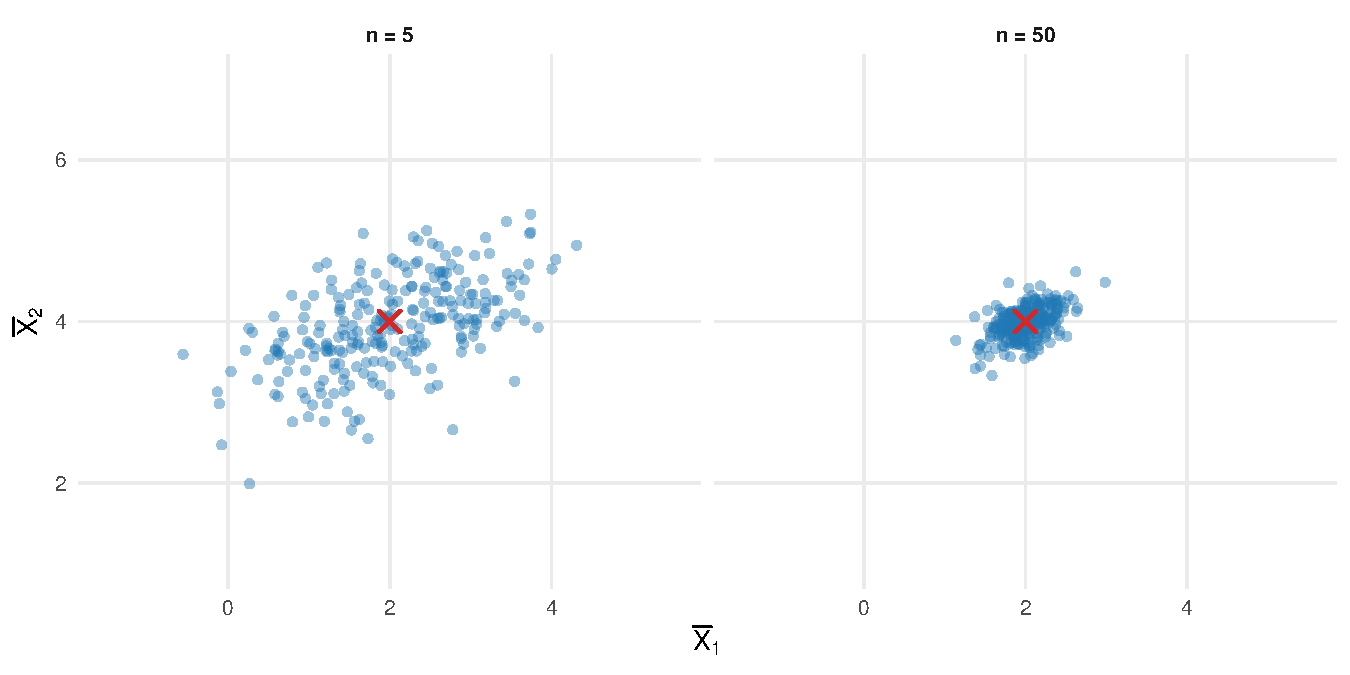
\includegraphics[keepaspectratio]{mod_2_amostrais_files/figure-pdf/fig-variabilidade-media-amostral-1.pdf}}

}

\caption{\label{fig-variabilidade-media-amostral}Vetores de médias
amostrais obtidos em 250 amostras de uma distribuição normal bivariada,
para tamanhos amostrais 5 e 50.}

\end{figure}%

Nos dois painéis, os vetores de médias amostrais se distribuem ao redor
de \(\boldsymbol{\mu}\). Para \(n=50\), a nuvem é mais concentrada do
que para \(n=5\), em concordância com a redução da matriz de
covariâncias por \(1/n\).

A figura \textbf{não representa ainda um resultado sobre a forma exata
da distribuição amostral de \(\bar{\boldsymbol{\mathsf X}}\)}. Essa
distribuição será estudada no Capítulo 12.

O vetor de médias amostrais estima a localização da população. A
estimação da dispersão exige considerar os desvios das observações em
relação a esse centro. Esses desvios conduzem à matriz SQPC e aos
estimadores da matriz de covariâncias.

\section{SQPC e estimação da matriz de
covariâncias}\label{sqpc-e-estimauxe7uxe3o-da-matriz-de-covariuxe2ncias}

O vetor de médias amostrais descreve a localização da amostra. A
estimação da matriz de covariâncias exige representar como as
observações se dispersam conjuntamente em torno desse centro.

O Capítulo 8 definiu a matriz total de somas de quadrados e produtos
cruzados (SQPC) na Definição~\ref{def-matriz-sscp-total} e a matriz de
covariâncias observada na
Definição~\ref{def-matriz-covariancias-observada}. A seção sobre métodos
de estimação mostrou ainda que o método dos momentos conduz à matriz
SQPC dividida por \(n\) e que, sob o modelo normal multivariado e as
condições de existência do máximo, a máxima verossimilhança conduz à
mesma expressão.

Nesta seção, a SQPC e as matrizes de covariâncias correspondentes passam
a ser tratadas como estatísticas aleatórias. O objetivo é comparar os
estimadores de \(\boldsymbol{\Sigma}\) resultantes de diferentes
critérios e estudar suas propriedades.

Considere a amostra aleatória multivariada definida na
Equação~\ref{eq-amostra-aleatoria-multivariada}, com unidades
independentes e

\[
E
\left(
\boldsymbol{\mathsf X}_i
\right)
=
\boldsymbol{\mu}
\]

e

\[
\operatorname{Cov}
\left(
\boldsymbol{\mathsf X}_i
\right)
=
\boldsymbol{\Sigma},
\qquad
i=1,\ldots,n,
\]

e suponha que os segundos momentos sejam finitos.

\subsection{SQPC como estatística
aleatória}\label{sqpc-como-estatuxedstica-aleatuxf3ria}

A matriz aleatória da amostra é

\[
\boldsymbol{\mathcal X}
=
\begin{bmatrix}
\boldsymbol{\mathsf X}_1^\top\\
\vdots\\
\boldsymbol{\mathsf X}_n^\top
\end{bmatrix}
\in
\mathbb R^{n\times p}.
\]

Retomando a matriz de centralização utilizada na
Equação~\ref{eq-centralizacao-por-hn},

\[
\mathbf H_n
=
\mathbf I_n
-
\frac{1}{n}
\mathbf 1_n
\mathbf 1_n^\top,
\]

define-se a matriz aleatória centralizada por

\begin{equation}\phantomsection\label{eq-matriz-amostral-centralizada-aleatoria}{
\boldsymbol{\mathcal X}_c
=
\mathbf H_n
\boldsymbol{\mathcal X}.
}\end{equation}

Suas linhas são

\[
\left(
\boldsymbol{\mathsf X}_i
-
\bar{\boldsymbol{\mathsf X}}
\right)^\top.
\]

\begin{definition}[Matriz SQPC
amostral]\protect\hypertarget{def-sscp-amostral-aleatoria}{}\label{def-sscp-amostral-aleatoria}

A \textbf{matriz de somas de quadrados e produtos cruzados (SQPC)
amostral} é a estatística

\begin{equation}\phantomsection\label{eq-sscp-amostral-aleatoria}{
\boldsymbol{\mathsf T}
=
\sum_{i=1}^{n}
\left(
\boldsymbol{\mathsf X}_i
-
\bar{\boldsymbol{\mathsf X}}
\right)
\left(
\boldsymbol{\mathsf X}_i
-
\bar{\boldsymbol{\mathsf X}}
\right)^\top.
}\end{equation}

Equivalentemente,

\begin{equation}\phantomsection\label{eq-sscp-amostral-forma-matricial}{
\boldsymbol{\mathsf T}
=
\boldsymbol{\mathcal X}_c^\top
\boldsymbol{\mathcal X}_c
=
\boldsymbol{\mathcal X}^\top
\mathbf H_n
\boldsymbol{\mathcal X}.
}\end{equation}

\end{definition}

Após a observação da amostra,

\[
\mathbf X_c
=
\mathbf H_n
\mathbf X
\]

e

\begin{equation}\phantomsection\label{eq-sscp-amostral-observada}{
\mathbf T
=
\mathbf X_c^\top
\mathbf X_c
=
\sum_{i=1}^{n}
\left(
\mathbf x_i-\bar{\mathbf x}
\right)
\left(
\mathbf x_i-\bar{\mathbf x}
\right)^\top.
}\end{equation}

A matriz \(\mathbf T\) é exatamente a matriz SQPC observada definida na
Definição~\ref{def-matriz-sscp-total} e escrita matricialmente na
Equação~\ref{eq-definicao-sscp-total}. A diferença de notação é
probabilística: \(\boldsymbol{\mathsf T}\) representa a estatística
aleatória, enquanto \(\mathbf T\) representa sua realização observada.

O elemento \((j,k)\) de \(\boldsymbol{\mathsf T}\) é

\begin{equation}\phantomsection\label{eq-elemento-sscp-amostral}{
\mathsf T_{jk}
=
\sum_{i=1}^{n}
\left(
X_{ij}-\bar X_j
\right)
\left(
X_{ik}-\bar X_k
\right).
}\end{equation}

Na diagonal,

\[
\mathsf T_{jj}
=
\sum_{i=1}^{n}
\left(
X_{ij}-\bar X_j
\right)^2
\]

é a soma de quadrados centralizada da variável \(j\). Fora da diagonal,
\(\mathsf T_{jk}\) é o produto cruzado centralizado entre as variáveis
\(j\) e \(k\).

Após a observação da amostra, os elementos correspondentes de
\(\mathbf T\) são denotados por \(t_{jk}\).

\subsection{Decomposição em torno de um centro
arbitrário}\label{decomposiuxe7uxe3o-em-torno-de-um-centro-arbitruxe1rio}

A caracterização do centroide na
Equação~\ref{eq-decomposicao-centroide-media} mostrou, em termos de
distâncias quadráticas, como a dispersão em torno de um centro
arbitrário pode ser decomposta em uma parcela em torno da média amostral
e outra associada ao deslocamento do centro. Para a estimação da matriz
de covariâncias, utiliza-se a versão matricial dessa decomposição.

\begin{proposition}[Decomposição da SQPC em torno de um centro
arbitrário]\protect\hypertarget{prp-decomposicao-sscp-centro-arbitrario}{}\label{prp-decomposicao-sscp-centro-arbitrario}

Para qualquer vetor fixo

\[
\mathbf c
\in
\mathbb R^p,
\]

tem-se

\begin{equation}\phantomsection\label{eq-decomposicao-sscp-centro-arbitrario}{
\begin{aligned}
&
\sum_{i=1}^{n}
\left(
\boldsymbol{\mathsf X}_i-\mathbf c
\right)
\left(
\boldsymbol{\mathsf X}_i-\mathbf c
\right)^\top
\\
&=
\boldsymbol{\mathsf T}
+
n
\left(
\bar{\boldsymbol{\mathsf X}}-\mathbf c
\right)
\left(
\bar{\boldsymbol{\mathsf X}}-\mathbf c
\right)^\top.
\end{aligned}
}\end{equation}

\end{proposition}

\begin{proof}
Escreva

\[
\boldsymbol{\mathsf X}_i-\mathbf c
=
\left(
\boldsymbol{\mathsf X}_i
-
\bar{\boldsymbol{\mathsf X}}
\right)
+
\left(
\bar{\boldsymbol{\mathsf X}}
-
\mathbf c
\right).
\]

Substituindo na soma dos produtos externos, surgem quatro parcelas. Os
dois termos cruzados contêm

\[
\sum_{i=1}^{n}
\left(
\boldsymbol{\mathsf X}_i
-
\bar{\boldsymbol{\mathsf X}}
\right)
=
\mathbf 0,
\]

e, portanto, se anulam. Restam

\[
\boldsymbol{\mathsf T}
\]

e

\[
n
\left(
\bar{\boldsymbol{\mathsf X}}-\mathbf c
\right)
\left(
\bar{\boldsymbol{\mathsf X}}-\mathbf c
\right)^\top,
\]

o que fornece Equação~\ref{eq-decomposicao-sscp-centro-arbitrario}.
\end{proof}

Para

\[
\mathbf c
=
\boldsymbol{\mu},
\]

obtém-se

\begin{equation}\phantomsection\label{eq-decomposicao-sscp-media-populacional}{
\begin{aligned}
&
\sum_{i=1}^{n}
\left(
\boldsymbol{\mathsf X}_i-\boldsymbol{\mu}
\right)
\left(
\boldsymbol{\mathsf X}_i-\boldsymbol{\mu}
\right)^\top
\\
&=
\boldsymbol{\mathsf T}
+
n
\left(
\bar{\boldsymbol{\mathsf X}}-\boldsymbol{\mu}
\right)
\left(
\bar{\boldsymbol{\mathsf X}}-\boldsymbol{\mu}
\right)^\top.
\end{aligned}
}\end{equation}

Essa identidade separa a dispersão das observações em torno do centro
populacional em duas parcelas: a dispersão em torno da média amostral e
o afastamento entre a média amostral e a média populacional.

\subsection{Esperança da SQPC}\label{esperanuxe7a-da-sqpc}

A identidade anterior permite obter a esperança de
\(\boldsymbol{\mathsf T}\) sem assumir normalidade.

\begin{proposition}[Esperança da
SQPC]\protect\hypertarget{prp-esperanca-sscp-amostral}{}\label{prp-esperanca-sscp-amostral}

Se

\[
\boldsymbol{\mathsf X}_1,
\ldots,
\boldsymbol{\mathsf X}_n
\]

são independentes e satisfazem

\[
E
\left(
\boldsymbol{\mathsf X}_i
\right)
=
\boldsymbol{\mu}
\]

e

\[
\operatorname{Cov}
\left(
\boldsymbol{\mathsf X}_i
\right)
=
\boldsymbol{\Sigma},
\qquad
i=1,\ldots,n,
\]

então

\begin{equation}\phantomsection\label{eq-esperanca-sscp-amostral}{
E
\left(
\boldsymbol{\mathsf T}
\right)
=
(n-1)
\boldsymbol{\Sigma}.
}\end{equation}

\end{proposition}

\begin{proof}
Tomando esperança no lado esquerdo de
Equação~\ref{eq-decomposicao-sscp-media-populacional},

\[
\begin{aligned}
E
\left[
\sum_{i=1}^{n}
\left(
\boldsymbol{\mathsf X}_i-\boldsymbol{\mu}
\right)
\left(
\boldsymbol{\mathsf X}_i-\boldsymbol{\mu}
\right)^\top
\right]
&=
\sum_{i=1}^{n}
\boldsymbol{\Sigma}
\\
&=
n
\boldsymbol{\Sigma}.
\end{aligned}
\]

Para a segunda parcela do lado direito,

\[
E
\left[
n
\left(
\bar{\boldsymbol{\mathsf X}}-\boldsymbol{\mu}
\right)
\left(
\bar{\boldsymbol{\mathsf X}}-\boldsymbol{\mu}
\right)^\top
\right]
=
n
\operatorname{Cov}
\left(
\bar{\boldsymbol{\mathsf X}}
\right).
\]

Por Equação~\ref{eq-covariancia-media-amostral},

\[
n
\operatorname{Cov}
\left(
\bar{\boldsymbol{\mathsf X}}
\right)
=
\boldsymbol{\Sigma}.
\]

Portanto,

\[
n
\boldsymbol{\Sigma}
=
E
\left(
\boldsymbol{\mathsf T}
\right)
+
\boldsymbol{\Sigma},
\]

e segue que

\[
E
\left(
\boldsymbol{\mathsf T}
\right)
=
(n-1)
\boldsymbol{\Sigma}.
\]
\end{proof}

O fator \(n-1\) surge porque a SQPC utiliza desvios em relação à média
estimada a partir da própria amostra. A centralização impõe

\[
\sum_{i=1}^{n}
\left(
\boldsymbol{\mathsf X}_i
-
\bar{\boldsymbol{\mathsf X}}
\right)
=
\mathbf0,
\]

de modo que os \(n\) vetores de desvios satisfazem uma restrição linear.
Assim, a centralização reduz em uma unidade a dimensão associada às
variações em torno da média amostral.

A relação

\[
E
\left(
\boldsymbol{\mathsf T}
\right)
=
(n-1)
\boldsymbol{\Sigma}
\]

depende apenas da independência entre as unidades amostrais e da
existência dos segundos momentos necessários; a normalidade multivariada
não é exigida. A distribuição completa de \(\boldsymbol{\mathsf T}\) sob
normalidade será tratada no Capítulo 12.

\subsection{Estimador não viesado da matriz de
covariâncias}\label{estimador-nuxe3o-viesado-da-matriz-de-covariuxe2ncias}

\begin{definition}[Matriz de covariâncias
amostral]\protect\hypertarget{def-matriz-covariancias-amostral-aleatoria}{}\label{def-matriz-covariancias-amostral-aleatoria}

Para \(n\geq2\), define-se

\begin{equation}\phantomsection\label{eq-matriz-covariancias-amostral-aleatoria}{
\boldsymbol{\mathsf S}
=
\frac{1}{n-1}
\boldsymbol{\mathsf T},
}\end{equation}

em que \(\boldsymbol{\mathsf T}\) é definida na
Definição~\ref{def-sscp-amostral-aleatoria}.

\end{definition}

\begin{proposition}[Não viesamento da matriz de covariâncias
amostral]\protect\hypertarget{prp-nao-viesamento-covariancia-amostral}{}\label{prp-nao-viesamento-covariancia-amostral}

Se

\[
\boldsymbol{\mathsf X}_1,
\ldots,
\boldsymbol{\mathsf X}_n
\]

são independentes, possuem segundos momentos finitos e satisfazem

\[
E
\left(
\boldsymbol{\mathsf X}_i
\right)
=
\boldsymbol{\mu}
\]

e

\[
\operatorname{Cov}
\left(
\boldsymbol{\mathsf X}_i
\right)
=
\boldsymbol{\Sigma},
\qquad
i=1,\ldots,n,
\]

então

\begin{equation}\phantomsection\label{eq-nao-viesamento-covariancia-amostral}{
E
\left(
\boldsymbol{\mathsf S}
\right)
=
\boldsymbol{\Sigma}.
}\end{equation}

Portanto, \(\boldsymbol{\mathsf S}\) é um estimador não viesado de
\(\boldsymbol{\Sigma}\).

\end{proposition}

\begin{proof}
Por Equação~\ref{eq-matriz-covariancias-amostral-aleatoria} e
Equação~\ref{eq-esperanca-sscp-amostral},

\[
\begin{aligned}
E
\left(
\boldsymbol{\mathsf S}
\right)
&=
\frac{1}{n-1}
E
\left(
\boldsymbol{\mathsf T}
\right)
\\
&=
\frac{1}{n-1}
(n-1)
\boldsymbol{\Sigma}
\\
&=
\boldsymbol{\Sigma}.
\end{aligned}
\]
\end{proof}

Após a observação, obtém-se a matriz de covariâncias observada definida
na Definição~\ref{def-matriz-covariancias-observada}:

\begin{equation}\phantomsection\label{eq-matriz-covariancias-amostral-observada}{
\mathbf S
=
\frac{1}{n-1}
\mathbf T.
}\end{equation}

Componente a componente,

\begin{equation}\phantomsection\label{eq-covariancia-amostral-elemento}{
\mathsf S_{jk}
=
\frac{1}{n-1}
\sum_{i=1}^{n}
\left(
X_{ij}-\bar X_j
\right)
\left(
X_{ik}-\bar X_k
\right).
}\end{equation}

Para \(j=k\),

\[
\mathsf S_{jj}
=
\frac{1}{n-1}
\sum_{i=1}^{n}
\left(
X_{ij}-\bar X_j
\right)^2
\]

é a variância amostral da variável \(j\).

Assim,

\[
\boldsymbol{\mathsf S}
=
\begin{bmatrix}
\mathsf S_{11} & \mathsf S_{12} & \cdots & \mathsf S_{1p}\\
\mathsf S_{21} & \mathsf S_{22} & \cdots & \mathsf S_{2p}\\
\vdots & \vdots & \ddots & \vdots\\
\mathsf S_{p1} & \mathsf S_{p2} & \cdots & \mathsf S_{pp}
\end{bmatrix}.
\]

Após a observação da amostra, os elementos correspondentes de
\(\mathbf S\) são denotados por \(s_{jk}\).

A divisão por \(n-1\) corrige o viés associado à centralização pela
média amostral. Ela não é escolhida para garantir semidefinição
positiva. Como a matriz SQPC observada satisfaz

\[
\mathbf T
=
\mathbf X_c^\top
\mathbf X_c,
\]

ela é uma matriz de Gram, conforme Definição~\ref{def-matriz-gram}, e
suas propriedades de simetria e semidefinição positiva decorrem da
Proposição~\ref{prp-propriedades-matriz-gram}. A multiplicação por
\(1/(n-1)>0\) preserva essas propriedades em \(\mathbf S\).

O não viesamento de \(\boldsymbol{\mathsf S}\) foi obtido utilizando
apenas segundos momentos. Uma caracterização de sua variabilidade
completa exigiria estudar

\[
\operatorname{Cov}
\left[
\operatorname{vec}
\left(
\boldsymbol{\mathsf S}
\right)
\right],
\]

utilizando o operador definido na Definição~\ref{def-operador-vec}. De
modo correspondente, o erro quadrático médio matricial sob a perda
baseada na norma de Frobenius definida na
Definição~\ref{def-norma-frobenius} envolveria

\[
E
\left[
\left\|
\boldsymbol{\mathsf S}
-
\boldsymbol{\Sigma}
\right\|_F^2
\right].
\]

Essas quantidades dependem, em geral, de momentos de quarta ordem. Por
isso, diferentemente do que ocorreu com o vetor de médias amostrais, os
segundos momentos assumidos nesta seção não são suficientes para
determinar a variabilidade completa ou o EQM de
\(\boldsymbol{\mathsf S}\). Sob normalidade, resultados mais específicos
serão obtidos a partir da distribuição amostral da matriz de
covariâncias no Capítulo 12.

\subsection{\texorpdfstring{Estimador com divisor \(n\): momentos e
máxima
verossimilhança}{Estimador com divisor n: momentos e máxima verossimilhança}}\label{estimador-com-divisor-n-momentos-e-muxe1xima-verossimilhanuxe7a}

Pelo método dos momentos, a
Equação~\ref{eq-estimador-momentos-covariancia-sscp} fornece

\[
\widehat{\boldsymbol{\Sigma}}_{\mathrm{MM}}
=
\frac{1}{n}
\boldsymbol{\mathsf T}.
\]

Sob o modelo normal multivariado não singular e quando o máximo existe,
a Equação~\ref{eq-mv-covariancia-normal} fornece a mesma estatística:

\[
\widehat{\boldsymbol{\Sigma}}_{\mathrm{MV}}
=
\frac{1}{n}
\boldsymbol{\mathsf T}.
\]

Portanto, no modelo normal e nas condições de existência do estimador de
máxima verossimilhança,

\[
\widehat{\boldsymbol{\Sigma}}_{\mathrm{MM}}
=
\widehat{\boldsymbol{\Sigma}}_{\mathrm{MV}}
=
\frac{1}{n}
\boldsymbol{\mathsf T}.
\]

Como

\[
\boldsymbol{\mathsf S}
=
\frac{1}{n-1}
\boldsymbol{\mathsf T},
\]

tem-se, sob o modelo normal,

\begin{equation}\phantomsection\label{eq-relacao-mv-covariancia-nao-viesada}{
\widehat{\boldsymbol{\Sigma}}_{\mathrm{MV}}
=
\frac{n-1}{n}
\boldsymbol{\mathsf S}.
}\end{equation}

Por Equação~\ref{eq-esperanca-sscp-amostral},

\[
E
\left(
\frac{\boldsymbol{\mathsf T}}{n}
\right)
=
\frac{n-1}{n}
\boldsymbol{\Sigma}.
\]

Portanto, como estimador de \(\boldsymbol{\Sigma}\),

\[
\operatorname{Bias}
\left(
\frac{\boldsymbol{\mathsf T}}{n}
\right)
=
-\frac{1}{n}
\boldsymbol{\Sigma}.
\]

Esse resultado vale para o estimador pelo método dos momentos sem exigir
normalidade. Sob o modelo normal e nas condições de existência do
máximo, a mesma estatística é também o estimador de máxima
verossimilhança. Nesse caso,

\begin{equation}\phantomsection\label{eq-vies-estimador-mv-covariancia}{
E
\left(
\widehat{\boldsymbol{\Sigma}}_{\mathrm{MV}}
\right)
=
\frac{n-1}{n}
\boldsymbol{\Sigma}
}\end{equation}

e

\begin{equation}\phantomsection\label{eq-vies-matricial-mv-covariancia}{
\operatorname{Bias}
\left(
\widehat{\boldsymbol{\Sigma}}_{\mathrm{MV}}
\right)
=
-\frac{1}{n}
\boldsymbol{\Sigma}.
}\end{equation}

Assim, o viés é uma propriedade da estatística
\(\boldsymbol{\mathsf T}/n\) como estimador de \(\boldsymbol{\Sigma}\),
e não uma consequência do método utilizado para obtê-la.

A comparação entre

\[
\frac{\boldsymbol{\mathsf T}}{n}
\qquad
\text{e}
\qquad
\frac{\boldsymbol{\mathsf T}}{n-1}
\]

mostra novamente que o princípio utilizado para construir um estimador e
suas propriedades estatísticas são questões distintas. A primeira matriz
resulta diretamente do método dos momentos e, sob normalidade, também da
máxima verossimilhança; a segunda utiliza a correção necessária para
obter não viesamento.

Quando \(n\) aumenta,

\[
\frac{n-1}{n}
\longrightarrow
1,
\]

de modo que a diferença relativa entre os dois estimadores desaparece.

\begin{tcolorbox}[enhanced jigsaw, colback=white, breakable, bottomrule=.15mm, left=2mm, arc=.35mm, rightrule=.15mm, colframe=quarto-callout-note-color-frame, toprule=.15mm, leftrule=.75mm, opacityback=0]

\vspace{-3mm}\textbf{Dois divisores, dois critérios}\vspace{3mm}

A matriz

\[
\frac{\boldsymbol{\mathsf T}}{n}
\]

surge como estimador de momentos e, sob o modelo normal e as condições
de existência do máximo, como estimador de máxima verossimilhança.

A matriz

\[
\frac{\boldsymbol{\mathsf T}}{n-1}
\]

é construída para satisfazer

\[
E
\left(
\boldsymbol{\mathsf S}
\right)
=
\boldsymbol{\Sigma}.
\]

Nenhum dos dois divisores é universalmente ``correto'' sem especificar o
critério de estimação.

\end{tcolorbox}

Sob o modelo normal multivariado,
Proposição~\ref{prp-suficiencia-normal-multivariada} estabeleceu que

\[
\left(
\bar{\boldsymbol{\mathsf X}},
\boldsymbol{\mathsf T}
\right)
\]

é suficiente para

\[
\left(
\boldsymbol{\mu},
\boldsymbol{\Sigma}
\right).
\]

Como, para \(n\) fixado,

\[
\boldsymbol{\mathsf S}
=
\frac{1}{n-1}
\boldsymbol{\mathsf T}
\]

é uma transformação bijetiva de \(\boldsymbol{\mathsf T}\), o par

\[
\left(
\bar{\boldsymbol{\mathsf X}},
\boldsymbol{\mathsf S}
\right)
\]

preserva a mesma informação sobre os parâmetros. Essa afirmação é
conjunta: ela não significa que \(\boldsymbol{\mathsf S}\) isoladamente
seja suficiente para \((\boldsymbol{\mu},\boldsymbol{\Sigma})\).

\subsection{Consistência dos estimadores de
covariância}\label{consistuxeancia-dos-estimadores-de-covariuxe2ncia}

O não viesamento é uma propriedade para tamanho amostral fixo. A
consistência descreve o comportamento quando \(n\) aumenta.

\begin{proposition}[Consistência da matriz de covariâncias
amostral]\protect\hypertarget{prp-consistencia-covariancia-amostral}{}\label{prp-consistencia-covariancia-amostral}

Considere uma amostra aleatória i.i.d.

\[
\boldsymbol{\mathsf X}_1,
\ldots,
\boldsymbol{\mathsf X}_n,
\]

em que

\[
\boldsymbol{\mathsf X}_i
\in
\mathbb R^p,
\]

com

\[
E
\left(
\boldsymbol{\mathsf X}_i
\right)
=
\boldsymbol{\mu},
\]

\[
\operatorname{Cov}
\left(
\boldsymbol{\mathsf X}_i
\right)
=
\boldsymbol{\Sigma},
\]

e

\[
E
\left(
\left\|
\boldsymbol{\mathsf X}_i
\right\|^2
\right)
<
\infty.
\]

Se o número \(p\) de variáveis permanece fixo quando \(n\to\infty\),
então

\begin{equation}\phantomsection\label{eq-consistencia-covariancia-amostral}{
\boldsymbol{\mathsf S}
\xrightarrow{P}
\boldsymbol{\Sigma}.
}\end{equation}

\end{proposition}

\begin{proof}
Pela identidade

\begin{equation}\phantomsection\label{eq-sscp-segundos-momentos-amostrais}{
\begin{aligned}
\frac{1}{n}
\boldsymbol{\mathsf T}
&=
\frac{1}{n}
\sum_{i=1}^{n}
\boldsymbol{\mathsf X}_i
\boldsymbol{\mathsf X}_i^\top
-
\bar{\boldsymbol{\mathsf X}}
\bar{\boldsymbol{\mathsf X}}^\top,
\end{aligned}
}\end{equation}

a matriz com divisor \(n\) pode ser escrita como diferença entre o
segundo momento amostral não central e o produto externo da média
amostral.

Para cada par \((j,k)\), a condição de segundos momentos finitos implica

\[
E
\left(
|X_jX_k|
\right)
<
\infty.
\]

Pela Lei dos Grandes Números,

\[
\frac{1}{n}
\sum_{i=1}^{n}
X_{ij}X_{ik}
\xrightarrow{P}
E
\left(
X_jX_k
\right),
\]

e

\[
\bar X_j
\xrightarrow{P}
\mu_j.
\]

Logo, elemento a elemento,

\[
\frac{1}{n}
\boldsymbol{\mathsf T}
\xrightarrow{P}
E
\left(
\boldsymbol{\mathsf X}
\boldsymbol{\mathsf X}^\top
\right)
-
\boldsymbol{\mu}
\boldsymbol{\mu}^\top
=
\boldsymbol{\Sigma}.
\]

Como \(p\) é fixo,

\[
\boldsymbol{\mathsf S}
=
\frac{n}{n-1}
\left(
\frac{\boldsymbol{\mathsf T}}{n}
\right)
\xrightarrow{P}
\boldsymbol{\Sigma}.
\]
\end{proof}

Pela mesma argumentação,

\begin{equation}\phantomsection\label{eq-consistencia-mv-covariancia}{
\widehat{\boldsymbol{\Sigma}}_{\mathrm{MV}}
=
\frac{\boldsymbol{\mathsf T}}{n}
\xrightarrow{P}
\boldsymbol{\Sigma}
}\end{equation}

sempre que a expressão é considerada como estatística. No modelo normal
positivo definido, sua interpretação como estimador de máxima
verossimilhança requer adicionalmente a existência do máximo discutida
anteriormente.

A consistência apresentada aqui corresponde ao regime clássico de
\textbf{dimensão fixa}. Quando \(p\) aumenta com \(n\), a convergência
deve ser analisada segundo o regime dimensional e a norma de interesse.

\subsection{Transformações, posto e
singularidade}\label{transformauxe7uxf5es-posto-e-singularidade}

As propriedades algébricas da matriz SQPC observada decorrem de sua
representação de Gram na Equação~\ref{eq-definicao-sscp-total} e do
limite de posto estabelecido na Equação~\ref{eq-posto-sscp-total}. Como
essas propriedades valem para cada realização da amostra, elas também
caracterizam as estatísticas \(\boldsymbol{\mathsf T}\) e
\(\boldsymbol{\mathsf S}\) amostra a amostra.

\textbf{Transformações afins.} A equivariância da matriz de covariâncias
amostral foi utilizada anteriormente como exemplo de
Definição~\ref{def-equivariancia-estimador}. Para referência, se

\[
\boldsymbol{\mathsf Y}_i
=
\mathbf C
\boldsymbol{\mathsf X}_i
+
\mathbf d,
\qquad
i=1,\ldots,n,
\]

então

\begin{equation}\phantomsection\label{eq-transformacao-sscp-amostral}{
\boldsymbol{\mathsf T}_Y
=
\mathbf C
\boldsymbol{\mathsf T}_X
\mathbf C^\top
}\end{equation}

e

\begin{equation}\phantomsection\label{eq-transformacao-covariancia-amostral}{
\boldsymbol{\mathsf S}_Y
=
\mathbf C
\boldsymbol{\mathsf S}_X
\mathbf C^\top.
}\end{equation}

A translação \(\mathbf d\) desaparece pela centralização. Como a matriz
populacional satisfaz, pela
Proposição~\ref{prp-transformacao-afim-covariancia},

\[
\boldsymbol{\Sigma}_Y
=
\mathbf C
\boldsymbol{\Sigma}_X
\mathbf C^\top,
\]

a transformação da estatística acompanha exatamente a transformação
correspondente do parâmetro.

\textbf{Simetria e semidefinição positiva.} Pela representação de Gram
na Equação~\ref{eq-definicao-sscp-total} e pelas propriedades de
matrizes de Gram na Proposição~\ref{prp-propriedades-matriz-gram}, para
qualquer realização da amostra,

\[
\mathbf T
=
\mathbf T^\top
\qquad
\text{e}
\qquad
\mathbf T
\succeq
\mathbf0.
\]

Como

\[
\mathbf S
=
\frac{1}{n-1}
\mathbf T,
\]

a matriz \(\mathbf S\) também é simétrica e positiva semidefinida.
Assim, em aritmética exata, o estimador não produz autovalores
negativos.

\textbf{Variância de combinações lineares.} Para qualquer

\[
\mathbf a
\in
\mathbb R^p,
\]

tem-se

\begin{equation}\phantomsection\label{eq-variancia-amostral-combinacao-linear}{
\mathbf a^\top
\boldsymbol{\mathsf S}
\mathbf a
=
\frac{1}{n-1}
\sum_{i=1}^{n}
\left[
\mathbf a^\top
\left(
\boldsymbol{\mathsf X}_i
-
\bar{\boldsymbol{\mathsf X}}
\right)
\right]^2.
}\end{equation}

A forma quadrática é a variância amostral da variável projetada

\[
\mathbf a^\top
\boldsymbol{\mathsf X}.
\]

Portanto,

\[
\mathbf a^\top
\boldsymbol{\mathsf S}
\mathbf a
=
0
\]

se, e somente se, os valores observados da combinação linear
\(\mathbf a^\top\boldsymbol{\mathsf X}_i\) são constantes na amostra.

\textbf{Posto.} Pelo resultado estabelecido na
Equação~\ref{eq-posto-sscp-total}, para qualquer realização da amostra,

\begin{equation}\phantomsection\label{eq-posto-sscp-amostral}{
\operatorname{posto}
\left(
\mathbf T
\right)
=
\operatorname{posto}
\left(
\mathbf X_c
\right)
\leq
\min
\left(
p,n-1
\right).
}\end{equation}

Como \(\mathbf S\) é obtida por multiplicação de \(\mathbf T\) por uma
constante positiva,

\begin{equation}\phantomsection\label{eq-posto-covariancia-amostral}{
\operatorname{posto}
\left(
\mathbf S
\right)
=
\operatorname{posto}
\left(
\mathbf T
\right).
}\end{equation}

Uma condição necessária para

\[
\mathbf S
\succ
\mathbf0
\]

é, portanto,

\[
n\geq p+1.
\]

Mesmo quando essa desigualdade é satisfeita, a definição positiva
depende de as colunas de \(\mathbf X_c\) possuírem posto completo.

Se

\[
p\geq n,
\]

então

\[
\operatorname{posto}
\left(
\mathbf S
\right)
\leq
n-1
<
p,
\]

e \(\mathbf S\) é necessariamente singular.

A singularidade significa que existe algum vetor não nulo

\[
\mathbf a
\in
\mathbb R^p
\]

tal que

\[
\mathbf S
\mathbf a
=
\mathbf0.
\]

Equivalentemente,

\[
\mathbf a^\top
\mathbf S
\mathbf a
=
0,
\]

de modo que a combinação linear correspondente apresenta variância
amostral nula.

\textbf{Inversão.} Quando

\[
\mathbf S
\succ
\mathbf0,
\]

sua inversa existe e pode ser utilizada em formas quadráticas e métricas
baseadas na covariância estimada.

Se \(\mathbf S\) é singular, \(\mathbf S^{-1}\) não existe. A utilização
de pseudoinversas ou de estimadores regularizados corresponde a escolhas
distintas e será discutida na seção de aprofundamento.

\begin{tcolorbox}[enhanced jigsaw, colback=white, breakable, bottomrule=.15mm, left=2mm, arc=.35mm, rightrule=.15mm, colframe=quarto-callout-caution-color-frame, toprule=.15mm, leftrule=.75mm, opacityback=0]

\vspace{-3mm}\textbf{Forma quadrática com covariância estimada}\vspace{3mm}

A distância de Mahalanobis foi definida na
Definição~\ref{def-distancia-mahalanobis} utilizando os parâmetros
populacionais. Sob normalidade,
Proposição~\ref{prp-mahalanobis-qui-quadrado} estabelece a distribuição
qui-quadrado da forma correspondente quando \(\boldsymbol{\mu}\) e
\(\boldsymbol{\Sigma}\) são conhecidos.

Substituir esses parâmetros por quantidades estimadas, como
\(\bar{\mathbf x}\) e \(\mathbf S\), produz outra estatística. Portanto,
a distribuição

\[
D_M^2
\sim
\chi_p^2
\]

não pode ser transferida diretamente para uma forma quadrática
construída com estimadores.

As distribuições apropriadas para estatísticas que envolvem parâmetros
estimados serão estudadas no Capítulo 12.

\end{tcolorbox}

Até este ponto, foram estabelecidas propriedades distintas dos
estimadores de \(\boldsymbol{\Sigma}\). A matriz
\(\boldsymbol{\mathsf S}=\boldsymbol{\mathsf T}/(n-1)\) é não viesada,
enquanto \(\boldsymbol{\mathsf T}/n\) é viesada em amostras finitas,
embora seja obtida pelo método dos momentos e, sob normalidade e
existência do máximo, também pela máxima verossimilhança. Ambos os
estimadores são consistentes no regime de dimensão fixa sob as condições
especificadas. Além disso, a matriz de covariâncias amostral é
equivariante sob transformações afins, positiva semidefinida em cada
realização e possui posto limitado por \(\min(p,n-1)\).

Esses resultados não estabelecem eficiência em amostras finitas, e a
avaliação completa da variabilidade ou do erro quadrático médio
matricial exige hipóteses adicionais sobre momentos de ordem superior.

O posto e a estabilidade numérica da matriz de covariâncias amostral
tornam-se especialmente relevantes quando \(p\) não é pequeno em relação
a \(n\). Antes de discutir esse regime, serão construídos os estimadores
correspondentes para covariâncias entre blocos e para correlações.

\section{Estimação de covariâncias cruzadas e
correlações}\label{estimauxe7uxe3o-de-covariuxe2ncias-cruzadas-e-correlauxe7uxf5es}

Em diversos problemas multivariados, as variáveis são organizadas em
blocos observados sobre as mesmas unidades amostrais. As covariâncias
cruzadas descrevem associações lineares entre variáveis pertencentes a
blocos distintos, enquanto as correlações removem as escalas marginais
dessas associações.

O Capítulo 8 definiu a matriz de covariâncias cruzadas populacional na
Definição~\ref{def-covariancia-cruzada}, a matriz de covariâncias
cruzadas observada na Definição~\ref{def-covariancia-cruzada-observada}
e a matriz de correlações observada na
Definição~\ref{def-matriz-correlacoes-observada}. Nesta seção, os
objetos correspondentes são tratados como estatísticas aleatórias e
utilizados na estimação de suas contrapartes populacionais.

\subsection{Covariâncias cruzadas entre
blocos}\label{covariuxe2ncias-cruzadas-entre-blocos}

Considere os vetores aleatórios

\[
\boldsymbol{\mathsf X}
\in
\mathbb R^p
\qquad
\text{e}
\qquad
\boldsymbol{\mathsf Y}
\in
\mathbb R^q.
\]

A matriz de covariâncias cruzadas populacional

\[
\boldsymbol{\Sigma}_{XY}
\]

foi definida na Definição~\ref{def-covariancia-cruzada}. Sua orientação
satisfaz, conforme Equação~\ref{eq-transposta-covariancia-cruzada},

\[
\boldsymbol{\Sigma}_{YX}
=
\boldsymbol{\Sigma}_{XY}^\top.
\]

Para o vetor conjunto

\[
\begin{bmatrix}
\boldsymbol{\mathsf X}\\
\boldsymbol{\mathsf Y}
\end{bmatrix},
\]

a estrutura em blocos da matriz de covariâncias segue
Equação~\ref{eq-covariancia-vetor-particionado}. Neste capítulo, será
denotada por

\begin{equation}\phantomsection\label{eq-covariancia-populacional-vetor-conjunto}{
\boldsymbol{\Sigma}_{\mathrm{conj}}
=
\begin{bmatrix}
\boldsymbol{\Sigma}_{XX}
&
\boldsymbol{\Sigma}_{XY}
\\
\boldsymbol{\Sigma}_{YX}
&
\boldsymbol{\Sigma}_{YY}
\end{bmatrix}.
}\end{equation}

Para estimar \(\boldsymbol{\Sigma}_{XY}\), é necessária uma amostra
\textbf{pareada}:

\[
\left(
\boldsymbol{\mathsf X}_1,
\boldsymbol{\mathsf Y}_1
\right),
\ldots,
\left(
\boldsymbol{\mathsf X}_n,
\boldsymbol{\mathsf Y}_n
\right),
\]

independente e identicamente distribuída segundo a distribuição conjunta
de

\[
\left(
\boldsymbol{\mathsf X},
\boldsymbol{\mathsf Y}
\right).
\]

O pareamento significa que \(\boldsymbol{\mathsf X}_i\) e
\(\boldsymbol{\mathsf Y}_i\) correspondem à mesma unidade amostral.
Alterar a correspondência entre as linhas dos dois blocos modifica as
covariâncias cruzadas.

Organize as observações nas matrizes aleatórias

\[
\boldsymbol{\mathcal X}
\in
\mathbb R^{n\times p}
\]

e

\[
\boldsymbol{\mathcal Y}
\in
\mathbb R^{n\times q}.
\]

Após a centralização,

\[
\boldsymbol{\mathcal X}_c
=
\mathbf H_n
\boldsymbol{\mathcal X}
\]

e

\[
\boldsymbol{\mathcal Y}_c
=
\mathbf H_n
\boldsymbol{\mathcal Y}.
\]

\begin{definition}[Matriz de somas de produtos cruzados entre
blocos]\protect\hypertarget{def-sscp-cruzada-amostral}{}\label{def-sscp-cruzada-amostral}

A \textbf{matriz de somas de produtos cruzados entre os dois blocos} é

\begin{equation}\phantomsection\label{eq-sscp-cruzada-forma-matricial}{
\boldsymbol{\mathsf T}_{XY}
=
\boldsymbol{\mathcal X}_c^\top
\boldsymbol{\mathcal Y}_c.
}\end{equation}

Equivalentemente,

\begin{equation}\phantomsection\label{eq-sscp-cruzada-somatorio}{
\boldsymbol{\mathsf T}_{XY}
=
\sum_{i=1}^{n}
\left(
\boldsymbol{\mathsf X}_i
-
\bar{\boldsymbol{\mathsf X}}
\right)
\left(
\boldsymbol{\mathsf Y}_i
-
\bar{\boldsymbol{\mathsf Y}}
\right)^\top.
}\end{equation}

\end{definition}

Após a observação,

\begin{equation}\phantomsection\label{eq-sscp-cruzada-estimada}{
\mathbf T_{XY}
=
\mathbf X_c^\top
\mathbf Y_c.
}\end{equation}

A inversão da ordem dos blocos produz

\[
\boldsymbol{\mathsf T}_{YX}
=
\boldsymbol{\mathsf T}_{XY}^\top
\]

e

\[
\mathbf T_{YX}
=
\mathbf T_{XY}^\top.
\]

\begin{definition}[Matriz de covariâncias cruzadas
amostral]\protect\hypertarget{def-covariancia-cruzada-amostral}{}\label{def-covariancia-cruzada-amostral}

Para \(n\geq2\), a matriz de covariâncias cruzadas amostral é

\begin{equation}\phantomsection\label{eq-covariancia-cruzada-amostral}{
\boldsymbol{\mathsf S}_{XY}
=
\frac{1}{n-1}
\boldsymbol{\mathsf T}_{XY},
}\end{equation}

em que \(\boldsymbol{\mathsf T}_{XY}\) é a matriz de somas de produtos
cruzados entre os blocos definida na
Definição~\ref{def-sscp-cruzada-amostral}.

\end{definition}

Após a observação da amostra, obtém-se a matriz de covariâncias cruzadas
observada definida na Definição~\ref{def-covariancia-cruzada-observada}:

\begin{equation}\phantomsection\label{eq-covariancia-cruzada-estimada}{
\mathbf S_{XY}
=
\frac{1}{n-1}
\mathbf T_{XY}
=
\frac{1}{n-1}
\mathbf X_c^\top
\mathbf Y_c.
}\end{equation}

Seu elemento \((j,k)\) é

\begin{equation}\phantomsection\label{eq-elemento-covariancia-cruzada}{
\mathsf S_{X_jY_k}
=
\frac{1}{n-1}
\sum_{i=1}^{n}
\left(
X_{ij}-\bar X_j
\right)
\left(
Y_{ik}-\bar Y_k
\right).
}\end{equation}

Após a observação da amostra, o elemento correspondente de
\(\mathbf S_{XY}\) é denotado por \(s_{X_jY_k}\).

\begin{proposition}[Não viesamento da covariância cruzada
amostral]\protect\hypertarget{prp-nao-vies-covariancia-cruzada}{}\label{prp-nao-vies-covariancia-cruzada}

Considere uma amostra pareada i.i.d. do vetor conjunto

\[
\begin{bmatrix}
\boldsymbol{\mathsf X}\\
\boldsymbol{\mathsf Y}
\end{bmatrix},
\]

com segundos momentos finitos. Então,

\begin{equation}\phantomsection\label{eq-esperanca-covariancia-cruzada}{
E
\left(
\boldsymbol{\mathsf S}_{XY}
\right)
=
\boldsymbol{\Sigma}_{XY}.
}\end{equation}

\end{proposition}

\begin{proof}
A matriz de covariâncias amostral do vetor conjunto é

\[
\boldsymbol{\mathsf S}_{\mathrm{conj}}
=
\begin{bmatrix}
\boldsymbol{\mathsf S}_{XX}
&
\boldsymbol{\mathsf S}_{XY}
\\
\boldsymbol{\mathsf S}_{YX}
&
\boldsymbol{\mathsf S}_{YY}
\end{bmatrix}.
\]

Pelo não viesamento da matriz de covariâncias amostral estabelecido na
Equação~\ref{eq-nao-viesamento-covariancia-amostral},

\[
E
\left(
\boldsymbol{\mathsf S}_{\mathrm{conj}}
\right)
=
\boldsymbol{\Sigma}_{\mathrm{conj}}.
\]

A igualdade entre os blocos superiores direitos fornece

\[
E
\left(
\boldsymbol{\mathsf S}_{XY}
\right)
=
\boldsymbol{\Sigma}_{XY}.
\]
\end{proof}

O método dos momentos aplicado à matriz de covariâncias do vetor
conjunto conduz ao estimador

\[
\widehat{\boldsymbol{\Sigma}}_{\mathrm{conj,MM}}
=
\frac{1}{n}
\boldsymbol{\mathsf T}_{\mathrm{conj}}.
\]

Consequentemente, o bloco correspondente à covariância cruzada é

\[
\widehat{\boldsymbol{\Sigma}}_{XY,\mathrm{MM}}
=
\frac{1}{n}
\boldsymbol{\mathsf T}_{XY}.
\]

Sob normalidade conjunta não singular,

\[
\begin{bmatrix}
\boldsymbol{\mathsf X}_i\\
\boldsymbol{\mathsf Y}_i
\end{bmatrix}
\overset{\mathrm{iid}}{\sim}
N_{p+q}
\left(
\begin{bmatrix}
\boldsymbol{\mu}_X\\
\boldsymbol{\mu}_Y
\end{bmatrix},
\boldsymbol{\Sigma}_{\mathrm{conj}}
\right),
\]

o estimador de máxima verossimilhança da matriz conjunta de
covariâncias, quando existe, utiliza também o divisor \(n\). Portanto,

\begin{equation}\phantomsection\label{eq-mv-covariancia-cruzada}{
\widehat{\boldsymbol{\Sigma}}_{XY,\mathrm{MM}}
=
\widehat{\boldsymbol{\Sigma}}_{XY,\mathrm{MV}}
=
\frac{1}{n}
\boldsymbol{\mathsf T}_{XY}
=
\frac{n-1}{n}
\boldsymbol{\mathsf S}_{XY}.
}\end{equation}

Se

\[
n\geq p+q+1
\]

e a distribuição normal conjunta é não singular, a matriz SQPC do vetor
conjunto possui posto \(p+q\) quase certamente. Nessas condições, o
estimador positivo definido de máxima verossimilhança da matriz conjunta
existe quase certamente.

Por Equação~\ref{eq-esperanca-covariancia-cruzada},

\[
E
\left(
\frac{1}{n}
\boldsymbol{\mathsf T}_{XY}
\right)
=
\frac{n-1}{n}
\boldsymbol{\Sigma}_{XY}.
\]

Assim,

\[
\operatorname{Bias}
\left(
\frac{1}{n}
\boldsymbol{\mathsf T}_{XY}
\right)
=
-\frac{1}{n}
\boldsymbol{\Sigma}_{XY}.
\]

Esse viés pertence à estatística \(\boldsymbol{\mathsf T}_{XY}/n\) como
estimador de \(\boldsymbol{\Sigma}_{XY}\) e não depende da hipótese de
normalidade. A normalidade é necessária apenas para interpretar essa
mesma estatística como o bloco cruzado do estimador de máxima
verossimilhança da matriz conjunta.

A consistência também pode ser obtida diretamente a partir da matriz de
covariâncias do vetor conjunto. Sob as condições da
Proposição~\ref{prp-consistencia-covariancia-amostral}, aplicadas ao
vetor de dimensão \(p+q\),

\[
\boldsymbol{\mathsf S}_{\mathrm{conj}}
\xrightarrow{P}
\boldsymbol{\Sigma}_{\mathrm{conj}}.
\]

Consequentemente, cada um de seus blocos converge para o bloco
populacional correspondente e, em particular,

\begin{equation}\phantomsection\label{eq-consistencia-covariancia-cruzada}{
\boldsymbol{\mathsf S}_{XY}
\xrightarrow{P}
\boldsymbol{\Sigma}_{XY}.
}\end{equation}

Como

\[
\frac{1}{n}
\boldsymbol{\mathsf T}_{XY}
=
\frac{n-1}{n}
\boldsymbol{\mathsf S}_{XY},
\]

também se obtém

\[
\frac{1}{n}
\boldsymbol{\mathsf T}_{XY}
\xrightarrow{P}
\boldsymbol{\Sigma}_{XY}.
\] A transformação da covariância cruzada amostral acompanha a
transformação do parâmetro populacional estabelecida na
Equação~\ref{eq-transformacao-covariancia-cruzada}. Se

\[
\boldsymbol{\mathsf U}
=
\mathbf C
\boldsymbol{\mathsf X}
+
\mathbf c
\]

e

\[
\boldsymbol{\mathsf V}
=
\mathbf D
\boldsymbol{\mathsf Y}
+
\mathbf d,
\]

então

\begin{equation}\phantomsection\label{eq-transformacao-covariancia-cruzada-amostral}{
\boldsymbol{\mathsf S}_{UV}
=
\mathbf C
\boldsymbol{\mathsf S}_{XY}
\mathbf D^\top.
}\end{equation}

Portanto, \(\boldsymbol{\mathsf S}_{XY}\) é equivariante em relação a
essas transformações afins dos dois blocos. Os vetores de localização
\(\mathbf c\) e \(\mathbf d\) desaparecem após a centralização.

Para

\[
U
=
\mathbf a^\top
\boldsymbol{\mathsf X}
\]

e

\[
V
=
\mathbf b^\top
\boldsymbol{\mathsf Y},
\]

segue que

\begin{equation}\phantomsection\label{eq-combinacoes-covariancia-cruzada}{
\mathsf S_{UV}
=
\mathbf a^\top
\boldsymbol{\mathsf S}_{XY}
\mathbf b.
}\end{equation} Diferentemente de uma matriz de covariâncias de um único
vetor, \(\boldsymbol{\mathsf S}_{XY}\) é, em geral, retangular quando
\(p\neq q\). Mesmo quando \(p=q\), ela não precisa ser simétrica. Os
dois blocos satisfazem

\[
\boldsymbol{\mathsf S}_{YX}
=
\boldsymbol{\mathsf S}_{XY}^{\top}.
\]

Por isso, propriedades como simetria e semidefinição positiva não devem
ser atribuídas isoladamente à matriz de covariâncias cruzadas. Essas
propriedades pertencem à matriz de covariâncias do vetor conjunto, da
qual \(\boldsymbol{\mathsf S}_{XY}\) é um bloco.

O posto satisfaz

\begin{equation}\phantomsection\label{eq-posto-covariancia-cruzada}{
\operatorname{posto}
\left(
\boldsymbol{\mathsf S}_{XY}
\right)
\leq
\min
\left(
p,q,n-1
\right).
}\end{equation}

Esse limite restringirá posteriormente técnicas que utilizam
simultaneamente dois conjuntos de variáveis.

\subsection{Matriz de correlações
amostral}\label{matriz-de-correlauxe7uxf5es-amostral}

A matriz de correlações amostral é obtida pela padronização das
covariâncias pelas variâncias marginais correspondentes.

Considere

\[
\boldsymbol{\mathsf S}
=
\left(
\mathsf S_{jk}
\right)
\]

e defina a matriz diagonal das variâncias amostrais por

\[
\boldsymbol{\mathsf D}_S
=
\operatorname{diag}
\left(
\mathsf S_{11},\ldots,\mathsf S_{pp}
\right).
\]

\begin{definition}[Matriz de correlações
amostral]\protect\hypertarget{def-matriz-correlacoes-amostral}{}\label{def-matriz-correlacoes-amostral}

Quando todas as variâncias amostrais são positivas, a matriz de
correlações amostral é

\begin{equation}\phantomsection\label{eq-matriz-correlacoes-amostral}{
\boldsymbol{\mathsf R}
=
\boldsymbol{\mathsf D}_S^{-1/2}
\boldsymbol{\mathsf S}
\boldsymbol{\mathsf D}_S^{-1/2},
}\end{equation}

em que

\[
\boldsymbol{\mathsf D}_S
=
\operatorname{diag}
\left(
\mathsf S_{11},
\ldots,
\mathsf S_{pp}
\right).
\]

\end{definition}

Após a observação da amostra, obtém-se a matriz \(\mathbf R\) definida
na Definição~\ref{def-matriz-correlacoes-observada}:

\begin{equation}\phantomsection\label{eq-matriz-correlacoes-estimada}{
\mathbf R
=
\mathbf D_S^{-1/2}
\mathbf S
\mathbf D_S^{-1/2},
}\end{equation}

em que

\[
\mathbf D_S
=
\operatorname{diag}
\left(
s_{11},\ldots,s_{pp}
\right).
\]

O elemento \((j,k)\) da estatística aleatória \(\boldsymbol{\mathsf R}\)
é

\begin{equation}\phantomsection\label{eq-correlacao-amostral}{
\mathsf R_{jk}
=
\frac{\mathsf S_{jk}}
{\sqrt{\mathsf S_{jj}\mathsf S_{kk}}}.
}\end{equation}

Após a observação da amostra, o elemento correspondente de \(\mathbf R\)
é

\[
r_{jk}
=
\frac{s_{jk}}
{\sqrt{s_{jj}s_{kk}}}.
\]

Consequentemente,

\[
\mathsf R_{jj}=1
\]

e, para a realização observada,

\[
r_{jj}=1.
\]

A interpretação geométrica da correlação observada foi estabelecida na
Equação~\ref{eq-correlacao-cosseno-colunas}, que identifica \(r_{jk}\)
com o cosseno do ângulo entre as colunas centralizadas e padronizadas.
Aqui, a ênfase recai sobre \(\boldsymbol{\mathsf R}\) como estatística
utilizada para estimar a matriz populacional
\(\boldsymbol{\mathcal R}\).

\begin{tcolorbox}[enhanced jigsaw, colback=white, breakable, bottomrule=.15mm, left=2mm, arc=.35mm, rightrule=.15mm, colframe=quarto-callout-caution-color-frame, toprule=.15mm, leftrule=.75mm, opacityback=0]

\vspace{-3mm}\textbf{Existência da correlação amostral}\vspace{3mm}

A correlação envolvendo uma variável não está definida quando sua
variância amostral é zero.

Se

\[
\mathsf S_{jj}=0
\]

a correspondente padronização não existe.

\end{tcolorbox}

\subsection{Propriedades estruturais}\label{propriedades-estruturais}

\begin{proposition}[Propriedades da matriz de correlações
amostral]\protect\hypertarget{prp-propriedades-matriz-correlacoes-amostral}{}\label{prp-propriedades-matriz-correlacoes-amostral}

Quando todas as variâncias amostrais são positivas,
\(\boldsymbol{\mathsf R}\) é:

\begin{enumerate}
\def\labelenumi{\arabic{enumi}.}
\tightlist
\item
  simétrica;
\item
  positiva semidefinida;
\item
  unitária na diagonal.
\end{enumerate}

Além disso,

\begin{equation}\phantomsection\label{eq-posto-correlacao-covariancia}{
\operatorname{posto}
\left(
\boldsymbol{\mathsf R}
\right)
=
\operatorname{posto}
\left(
\boldsymbol{\mathsf S}
\right).
}\end{equation}

Consequentemente,

\begin{equation}\phantomsection\label{eq-definicao-positiva-correlacao-covariancia}{
\boldsymbol{\mathsf R}
\succ
\mathbf0
\quad\Longleftrightarrow\quad
\boldsymbol{\mathsf S}
\succ
\mathbf0.
}\end{equation}

\end{proposition}

\begin{proof}
A simetria decorre da simetria de \(\boldsymbol{\mathsf S}\).

Para qualquer \(\mathbf a\in\mathbb R^p\),

\[
\begin{aligned}
\mathbf a^\top
\boldsymbol{\mathsf R}
\mathbf a
&=
\left(
\boldsymbol{\mathsf D}_S^{-1/2}
\mathbf a
\right)^\top
\boldsymbol{\mathsf S}
\left(
\boldsymbol{\mathsf D}_S^{-1/2}
\mathbf a
\right)
\\
&\geq
0.
\end{aligned}
\]

Logo, \(\boldsymbol{\mathsf R}\) é positiva semidefinida.

A diagonal unitária decorre de

\[
\mathsf R_{jj}
=
\frac{\mathsf S_{jj}}{\mathsf S_{jj}}
=
1.
\]

Como \(\boldsymbol{\mathsf D}_S^{-1/2}\) é invertível, a transformação
por congruência preserva o posto e a definitude positiva.
\end{proof}

Uma matriz simétrica com diagonal unitária e elementos em \([-1,1]\) não
é necessariamente uma matriz de correlações válida. A positividade
semidefinida também é necessária.

Como

\[
\operatorname{posto}
\left(
\boldsymbol{\mathsf R}
\right)
=
\operatorname{posto}
\left(
\boldsymbol{\mathsf S}
\right),
\]

uma condição necessária para definitude positiva é

\[
n\geq p+1.
\]

Essa condição não é suficiente para uma amostra arbitrária, pois ainda
podem existir dependências lineares entre as colunas centralizadas.

Quando

\[
p\geq n,
\]

a matriz de correlações, se definida, é necessariamente singular.

Para uma realização observada,

\begin{equation}\phantomsection\label{eq-determinante-correlacao-amostral}{
\det
\left(
\mathbf R
\right)
=
\frac{
\det
\left(
\mathbf S
\right)
}{
\prod_{j=1}^{p}
s_{jj}
}.
}\end{equation}

A padronização remove as escalas marginais, mas não altera o posto.

A matriz de correlações populacional é uma função da matriz de
covariâncias,

\[
\boldsymbol{\mathcal R}
=
\mathbf D_{\Sigma}^{-1/2}
\boldsymbol{\Sigma}
\mathbf D_{\Sigma}^{-1/2}.
\]

Substituindo \(\boldsymbol{\Sigma}\) pelo estimador de momentos

\[
\widehat{\boldsymbol{\Sigma}}_{\mathrm{MM}}
=
\frac{1}{n}
\boldsymbol{\mathsf T},
\]

obtém-se um estimador por substituição de \(\boldsymbol{\mathcal R}\).
Como o fator comum \(1/n\) aparece tanto nas covariâncias quanto nas
variâncias marginais, ele se cancela na padronização. A matriz
resultante é

\[
\boldsymbol{\mathsf R}.
\]

Assim, \(\boldsymbol{\mathsf R}\) pode ser obtida pela padronização do
estimador de momentos de \(\boldsymbol{\Sigma}\).

Sob o modelo normal multivariado, quando o estimador de máxima
verossimilhança de \(\boldsymbol{\Sigma}\) existe,

\[
\widehat{\boldsymbol{\Sigma}}_{\mathrm{MV}}
=
\frac{n-1}{n}
\boldsymbol{\mathsf S}.
\]

Novamente, o fator comum \((n-1)/n\) cancela-se na transformação de
covariâncias em correlações. Pela
Proposição~\ref{prp-invariancia-maxima-verossimilhanca},

\begin{equation}\phantomsection\label{eq-mv-correlacao-amostral}{
\widehat{\boldsymbol{\mathcal R}}_{\mathrm{MV}}
=
\boldsymbol{\mathsf R}.
}\end{equation}

Assim, no modelo normal considerado e nas condições de existência do
máximo, a mesma matriz de correlações amostral também é obtida pela
máxima verossimilhança.

Essa coincidência não implica não viesamento. Em geral,

\[
E
\left(
\mathsf R_{jk}
\right)
\neq
\rho_{jk}.
\]

A razão é que a correlação amostral é uma função não linear das
variâncias e covariâncias amostrais.

Por outro lado, se

\[
\boldsymbol{\mathsf S}
\xrightarrow{P}
\boldsymbol{\Sigma}
\]

e

\[
\sigma_{jj}>0,
\qquad
j=1,\ldots,p,
\]

Considere a transformação

\[
g
\left(
\mathbf A
\right)
=
\mathbf D_A^{-1/2}
\mathbf A
\mathbf D_A^{-1/2},
\]

em que

\[
\mathbf D_A
=
\operatorname{diag}
\left(
a_{11},\ldots,a_{pp}
\right).
\]

Essa transformação converte uma matriz de covariâncias em sua matriz de
correlações e é contínua quando os elementos de sua diagonal são
positivos.

O \textbf{teorema do mapeamento contínuo} estabelece que, se uma
sequência de estatísticas converge em probabilidade e uma função é
contínua no limite, então a sequência obtida pela aplicação dessa função
também converge em probabilidade (Vaart, 1998).

Como

\[
\boldsymbol{\mathsf S}
\xrightarrow{P}
\boldsymbol{\Sigma}
\]

no regime de dimensão fixa e

\[
\sigma_{jj}>0,
\qquad
j=1,\ldots,p,
\]

a transformação \(g\) é contínua em \(\boldsymbol{\Sigma}\). Portanto,

\[
g
\left(
\boldsymbol{\mathsf S}
\right)
\xrightarrow{P}
g
\left(
\boldsymbol{\Sigma}
\right).
\]

Como

\[
g
\left(
\boldsymbol{\mathsf S}
\right)
=
\boldsymbol{\mathsf R}
\]

e

\[
g
\left(
\boldsymbol{\Sigma}
\right)
=
\boldsymbol{\mathcal R},
\]

segue que

\begin{equation}\phantomsection\label{eq-consistencia-matriz-correlacoes}{
\boldsymbol{\mathsf R}
\xrightarrow{P}
\boldsymbol{\mathcal R}.
}\end{equation}

Portanto, a matriz de correlações amostral é consistente para a matriz
de correlações populacional, embora suas entradas possam ser viesadas em
amostras finitas.

\subsection{Transformações de localização e
escala}\label{transformauxe7uxf5es-de-localizauxe7uxe3o-e-escala}

O efeito populacional das mudanças de localização e escala sobre a
correlação foi estabelecido na
Equação~\ref{eq-correlacao-mudanca-escala}. Para uma realização
observada, considere

\[
y_{ij}
=
a_j+b_jx_{ij},
\qquad
b_j\neq0.
\]

A localização \(a_j\) desaparece após a centralização. Para duas
variáveis transformadas,

\begin{equation}\phantomsection\label{eq-transformacao-correlacao-amostral}{
r_{Y_jY_k}
=
\operatorname{sgn}
\left(
b_j
\right)
\operatorname{sgn}
\left(
b_k
\right)
r_{X_jX_k}.
}\end{equation}

Fatores de escala positivos preservam a correlação. Quando apenas um dos
fatores \(b_j\) e \(b_k\) é negativo, o sinal da correlação é invertido.
Mudanças de localização não alteram a correlação.

Em forma matricial, para

\[
\mathbf Y
=
\mathbf X\mathbf D_b
+
\mathbf 1_n\mathbf a^\top,
\]

com

\[
\mathbf D_b
=
\operatorname{diag}
\left(
b_1,\ldots,b_p
\right),
\]

defina

\[
\mathbf D_{\operatorname{sgn}}
=
\operatorname{diag}
\left[
\operatorname{sgn}(b_1),
\ldots,
\operatorname{sgn}(b_p)
\right].
\]

Então,

\begin{equation}\phantomsection\label{eq-transformacao-matricial-correlacoes}{
\mathbf R_Y
=
\mathbf D_{\operatorname{sgn}}
\mathbf R_X
\mathbf D_{\operatorname{sgn}}.
}\end{equation}

Se todos os fatores de escala são positivos,

\[
\mathbf R_Y
=
\mathbf R_X.
\]

Para dois blocos, defina as matrizes diagonais aleatórias

\[
\boldsymbol{\mathsf D}_X
=
\operatorname{diag}
\left(
\mathsf S_{X_1X_1},
\ldots,
\mathsf S_{X_pX_p}
\right)
\]

e

\[
\boldsymbol{\mathsf D}_Y
=
\operatorname{diag}
\left(
\mathsf S_{Y_1Y_1},
\ldots,
\mathsf S_{Y_qY_q}
\right).
\]

Quando todas as variâncias amostrais envolvidas são positivas, define-se
a matriz de correlações cruzadas amostral por

\begin{equation}\phantomsection\label{eq-correlacao-cruzada-amostral}{
\boldsymbol{\mathsf R}_{XY}
=
\boldsymbol{\mathsf D}_X^{-1/2}
\boldsymbol{\mathsf S}_{XY}
\boldsymbol{\mathsf D}_Y^{-1/2}.
}\end{equation}

Seu elemento \((j,k)\) é

\[
\mathsf R_{X_jY_k}
=
\frac{
\mathsf S_{X_jY_k}
}{
\sqrt{
\mathsf S_{X_jX_j}
\mathsf S_{Y_kY_k}
}
}.
\]

Após a observação da amostra,

\[
\mathbf R_{XY}
=
\mathbf D_X^{-1/2}
\mathbf S_{XY}
\mathbf D_Y^{-1/2},
\]

em que

\[
\mathbf D_X
=
\operatorname{diag}
\left(
s_{X_1X_1},
\ldots,
s_{X_pX_p}
\right)
\]

e

\[
\mathbf D_Y
=
\operatorname{diag}
\left(
s_{Y_1Y_1},
\ldots,
s_{Y_qY_q}
\right).
\]

Seu elemento observado é

\[
r_{X_jY_k}
=
\frac{
s_{X_jY_k}
}{
\sqrt{
s_{X_jX_j}s_{Y_kY_k}
}
}.
\]

Além disso,

\[
\boldsymbol{\mathsf R}_{YX}
=
\boldsymbol{\mathsf R}_{XY}^{\top}
\]

e, após a observação,

\[
\mathbf R_{YX}
=
\mathbf R_{XY}^{\top}.
\]

A matriz de correlações do vetor conjunto assume a forma

\begin{equation}\phantomsection\label{eq-correlacao-vetor-conjunto}{
\mathbf R_{\mathrm{conj}}
=
\begin{bmatrix}
\mathbf R_{XX}
&
\mathbf R_{XY}
\\
\mathbf R_{YX}
&
\mathbf R_{YY}
\end{bmatrix}.
}\end{equation}

Até este ponto, foram estabelecidas propriedades distintas das
estatísticas utilizadas para representar associações entre variáveis. A
matriz \(\boldsymbol{\mathsf S}_{XY}\) é não viesada e consistente para
\(\boldsymbol{\Sigma}_{XY}\) sob as condições especificadas, enquanto
\(\boldsymbol{\mathsf T}_{XY}/n\) apresenta o mesmo fator de viés
observado na estimação da matriz de covariâncias e, sob normalidade
conjunta e existência do máximo, também corresponde ao estimador de
máxima verossimilhança do bloco cruzado.

A matriz de correlações amostral \(\boldsymbol{\mathsf R}\) remove as
escalas marginais, preserva a semidefinição positiva e o posto da matriz
de covariâncias quando está definida, é consistente no regime de
dimensão fixa, mas suas entradas não são, em geral, estimadores não
viesados das correlações populacionais. Sob o modelo normal, a
invariância da máxima verossimilhança conduz à mesma matriz
\(\boldsymbol{\mathsf R}\).

As matrizes de covariâncias e correlações cruzadas serão utilizadas
posteriormente em métodos que relacionam dois conjuntos de variáveis. O
objetivo neste capítulo é estabelecer sua estimação e as propriedades
necessárias para esses desenvolvimentos.

A próxima seção examina situações em que a dimensão, a redundância ou a
sensibilidade das estatísticas clássicas dificultam a estimação da
matriz de covariâncias.

\section{Aprofundamento: dimensão, estabilidade e extensões da
estimação}\label{aprofundamento-dimensuxe3o-estabilidade-e-extensuxf5es-da-estimauxe7uxe3o}

Esta seção examina situações em que a dimensão, o condicionamento ou a
sensibilidade das estatísticas amostrais exigem cuidados adicionais. Os
resultados anteriores trataram dos estimadores clássicos da média e da
matriz de covariâncias. A regularização e a estimação robusta modificam
esses procedimentos para tratar, respectivamente, problemas de
instabilidade e de sensibilidade.

Uma matriz de covariâncias não estruturada de um vetor com \(p\)
componentes possui

\[
\frac{p(p+1)}{2}
\]

parâmetros distintos. Assim, o número de parâmetros de dispersão a
estimar cresce quadraticamente com \(p\), enquanto o número de unidades
amostrais permanece igual a \(n\).

Regularização e robustez respondem a problemas diferentes. A
regularização procura reduzir a instabilidade associada à dimensão, à
redundância, ao tamanho amostral ou ao mau condicionamento. A estimação
robusta procura reduzir a sensibilidade do procedimento a determinadas
formas de contaminação ou desvios do modelo. As duas abordagens podem
ser combinadas, mas tratam de problemas distintos.

\subsection{\texorpdfstring{Relação entre \(p\) e
\(n\)}{Relação entre p e n}}\label{relauxe7uxe3o-entre-p-e-n}

O limite de posto estabelecido na Equação~\ref{eq-posto-sscp-amostral},

\[
\operatorname{posto}
\left(
\boldsymbol{\mathsf S}
\right)
\leq
\min
\left(
p,n-1
\right),
\]

permite distinguir diferentes regimes dimensionais.

\textbf{Dimensão fixa.} No regime clássico,

\[
p
\]

permanece fixo enquanto

\[
n\longrightarrow\infty.
\]

Sob as condições da
Proposição~\ref{prp-consistencia-covariancia-amostral},

\[
\boldsymbol{\mathsf S}
\xrightarrow{P}
\boldsymbol{\Sigma}.
\]

Como \(p\) é fixo, a convergência dos elementos implica convergência em
qualquer norma matricial sobre \(\mathbb R^{p\times p}\), pois todas
essas normas são equivalentes em dimensão finita.

\textbf{Dimensão crescente.} Quando

\[
p=p_n
\]

também aumenta com \(n\), os resultados obtidos para dimensão fixa não
podem ser transferidos automaticamente. Um regime de referência é

\[
\frac{p_n}{n}
\longrightarrow
c,
\qquad
0<c<1.
\]

Nesse regime, a matriz de covariâncias amostral pode possuir posto
completo e, ainda assim, apresentar elevada variabilidade em seu
espectro.

O controle dos erros de estimação elemento a elemento não garante, por
si só, controle do erro matricial em norma espectral. Consequentemente,
boa estimação das covariâncias individuais não assegura automaticamente
boa estimação dos autovalores, autovetores, determinante, inversa ou
formas quadráticas que dependem da matriz inversa.

Além disso, o número de covariâncias fora da diagonal é

\[
\frac{p(p-1)}{2},
\]

e todas são estimadas a partir das mesmas \(n\) unidades.

Não existe um valor universal de \(p/n\) que separe matrizes estáveis e
instáveis. O comportamento depende também da estrutura de
\(\boldsymbol{\Sigma}\), da separação entre seus autovalores, da
distribuição populacional e da função da matriz utilizada
posteriormente.

\textbf{Dimensão maior ou igual ao tamanho amostral.} Se

\[
p\geq n,
\]

Equação~\ref{eq-posto-sscp-amostral} implica

\[
\operatorname{posto}
\left(
\boldsymbol{\mathsf S}
\right)
\leq
n-1
<
p.
\]

Logo, a matriz de covariâncias amostral é necessariamente singular.

Essa singularidade não implica singularidade de \(\boldsymbol{\Sigma}\).
Ela pode decorrer exclusivamente do número limitado de direções
amostrais disponíveis após a centralização.

\begin{tcolorbox}[enhanced jigsaw, colback=white, breakable, bottomrule=.15mm, left=2mm, arc=.35mm, rightrule=.15mm, colframe=quarto-callout-caution-color-frame, toprule=.15mm, leftrule=.75mm, opacityback=0]

\vspace{-3mm}\textbf{Posto amostral e posto populacional}\vspace{3mm}

Quando

\[
p\geq n,
\]

\(\boldsymbol{\mathsf S}\) é singular por construção, mesmo que a matriz
populacional satisfaça

\[
\boldsymbol{\Sigma}\succ\mathbf0.
\]

A singularidade da matriz amostral, portanto, não constitui evidência
suficiente de singularidade da matriz de covariâncias populacional.

\end{tcolorbox}

\subsection{Condicionamento e
inversão}\label{condicionamento-e-inversuxe3o}

Considere uma realização positiva definida,

\[
\mathbf S
=
\mathbf Q
\boldsymbol{\Lambda}
\mathbf Q^\top,
\]

com

\[
\boldsymbol{\Lambda}
=
\operatorname{diag}
\left(
\ell_1,\ldots,\ell_p
\right),
\]

e

\[
\ell_1
\geq
\cdots
\geq
\ell_p
>
0.
\]

A inversa é

\[
\mathbf S^{-1}
=
\mathbf Q
\boldsymbol{\Lambda}^{-1}
\mathbf Q^\top.
\]

Autovalores pequenos de \(\mathbf S\) tornam-se pesos elevados em
\(\mathbf S^{-1}\).

O número de condição espectral foi definido na
Definição~\ref{def-numero-condicao-svd}. Para uma matriz simétrica
positiva definida,

\begin{equation}\phantomsection\label{eq-numero-condicao-covariancia}{
\kappa_2
\left(
\mathbf S
\right)
=
\frac{
\ell_{\max}
\left(
\mathbf S
\right)
}{
\ell_{\min}
\left(
\mathbf S
\right)
}.
}\end{equation}

Quanto maior essa razão, maior é a diferença entre as escalas espectrais
extremas da matriz. Quando

\[
\ell_{\min}
\left(
\mathbf S
\right)
\longrightarrow
0,
\]

tem-se

\[
\kappa_2
\left(
\mathbf S
\right)
\longrightarrow
\infty.
\]

Se \(\mathbf S\) é singular, o número de condição associado à inversão é
infinito. Portanto, invertibilidade e bom condicionamento são
propriedades distintas.

O mau condicionamento torna a inversa sensível a erros de estimação:
pequenas perturbações em \(\mathbf S\) podem produzir alterações
acentuadas em

\[
\mathbf S^{-1}.
\]

O determinante também depende de todo o espectro:

\[
\det
\left(
\mathbf S
\right)
=
\prod_{j=1}^{p}
\ell_j.
\]

Já a estabilidade dos autovetores depende não somente da magnitude dos
autovalores, mas também de sua separação. Autovalores muito próximos
podem produzir direções individuais sensíveis a pequenas perturbações.

Considere, por exemplo, a contraparte amostral da forma quadrática
utilizada na distância de Mahalanobis definida na
Definição~\ref{def-distancia-mahalanobis}:

\[
d_{\mathbf S}^2
\left(
\mathbf x,
\bar{\mathbf x}
\right)
=
\left(
\mathbf x-\bar{\mathbf x}
\right)^\top
\mathbf S^{-1}
\left(
\mathbf x-\bar{\mathbf x}
\right).
\]

Nas coordenadas dos autovetores de \(\mathbf S\),

\[
d_{\mathbf S}^2
\left(
\mathbf x,
\bar{\mathbf x}
\right)
=
\sum_{j=1}^{p}
\frac{z_j^2}{\ell_j}.
\]

Assim, erros na estimação de autovalores pequenos podem ser amplificados
pela inversão, pois essas direções recebem pesos proporcionais a
\(1/\ell_j\).

\begin{tcolorbox}[enhanced jigsaw, colback=white, breakable, bottomrule=.15mm, left=2mm, arc=.35mm, rightrule=.15mm, colframe=quarto-callout-note-color-frame, toprule=.15mm, leftrule=.75mm, opacityback=0]

\vspace{-3mm}\textbf{Inversão computacional}\vspace{3mm}

A existência de \(\mathbf S^{-1}\) não significa que seja necessário
formá-la explicitamente.

Quando o objetivo é calcular

\[
\mathbf S^{-1}\mathbf b,
\]

é preferível, em geral, resolver o sistema

\[
\mathbf S\mathbf x
=
\mathbf b.
\]

Essa escolha não elimina o mau condicionamento, mas evita uma inversão
explícita desnecessária.

\end{tcolorbox}

\subsection{Regularização}\label{regularizauxe7uxe3o}

A regularização substitui a matriz de covariâncias amostral por um
estimador que combina \(\boldsymbol{\mathsf S}\) com restrições ou
valores de referência previamente especificados. O objetivo pode ser
reduzir variabilidade, melhorar o condicionamento ou produzir uma matriz
invertível.

Uma classe simples combina \(\boldsymbol{\mathsf S}\) com uma
matriz-alvo (Ledoit; Wolf, 2004).

\begin{definition}[Estimador de covariância por
contração]\protect\hypertarget{def-estimador-contracao-covariancia}{}\label{def-estimador-contracao-covariancia}

Considere uma matriz-alvo fixada

\[
\boldsymbol{\Gamma}
\in
\mathbb R^{p\times p},
\qquad
\boldsymbol{\Gamma}
\succeq
\mathbf0,
\]

e um peso

\[
0\leq\lambda\leq1.
\]

Define-se o estimador por contração

\begin{equation}\phantomsection\label{eq-estimador-contracao-covariancia}{
\widehat{\boldsymbol{\Sigma}}_{\lambda}
=
(1-\lambda)
\boldsymbol{\mathsf S}
+
\lambda
\boldsymbol{\Gamma}.
}\end{equation}

\end{definition}

Para

\[
\lambda=0,
\]

recupera-se \(\boldsymbol{\mathsf S}\). Para

\[
\lambda=1,
\]

o estimador coincide com o alvo.

A contração geralmente introduz viés. Sua avaliação deve considerar
conjuntamente viés e variabilidade por meio de uma função de perda e do
risco correspondente.

A consistência também depende da forma como a regularização varia com o
tamanho amostral. Se \(\lambda\in(0,1]\) e \(\boldsymbol{\Gamma}\) são
fixos e

\[
\boldsymbol{\mathsf S}
\xrightarrow{P}
\boldsymbol{\Sigma},
\]

então

\[
\widehat{\boldsymbol{\Sigma}}_{\lambda}
\xrightarrow{P}
(1-\lambda)
\boldsymbol{\Sigma}
+
\lambda
\boldsymbol{\Gamma}.
\]

Portanto, com \(\lambda>0\) fixo, o estimador não é, em geral,
consistente para \(\boldsymbol{\Sigma}\). Se a matriz-alvo
\(\boldsymbol{\Gamma}\) é fixa e o peso passa a depender de \(n\), com

\[
\lambda_n
\longrightarrow
0,
\]

então

\[
\widehat{\boldsymbol{\Sigma}}_{\lambda_n}
=
(1-\lambda_n)
\boldsymbol{\mathsf S}
+
\lambda_n
\boldsymbol{\Gamma}
\xrightarrow{P}
\boldsymbol{\Sigma},
\]

sempre que

\[
\boldsymbol{\mathsf S}
\xrightarrow{P}
\boldsymbol{\Sigma}.
\]

Assim, nesse caso, a intensidade da regularização desaparece
assintoticamente e a consistência da matriz de covariâncias amostral é
preservada.

Em aplicações, o alvo e o peso podem ser estimados a partir dos próprios
dados. Nesse caso,

\begin{equation}\phantomsection\label{eq-contracao-alvo-estimado}{
\widehat{\boldsymbol{\Sigma}}_{\widehat{\lambda}}
=
\left(
1-\widehat{\lambda}
\right)
\boldsymbol{\mathsf S}
+
\widehat{\lambda}
\widehat{\boldsymbol{\Gamma}}.
}\end{equation}

A aleatoriedade de \(\widehat{\lambda}\) e de
\(\widehat{\boldsymbol{\Gamma}}\) passa, então, a fazer parte das
propriedades do estimador.

A matriz-alvo precisa ser compatível com as unidades e escalas das
variáveis. Um alvo diagonal preserva as escalas marginais e reduz as
covariâncias. Um alvo esférico \(\tau\mathbf I_p\) pressupõe que uma
escala comum possua interpretação. Para matrizes de correlações, a
identidade \(\mathbf I_p\) constitui uma escolha natural de referência.
O alvo também pode representar relações previamente especificadas entre
as variáveis, como covariâncias nulas ou uma estrutura de correlação
definida antes da estimação.

A identidade \(\mathbf I_p\) não é um alvo neutro para uma matriz de
covariâncias quando as variáveis são medidas em unidades ou escalas
distintas.

Um alvo esférico adaptado à escala observada pode utilizar

\begin{equation}\phantomsection\label{eq-variancia-media-alvo-contracao}{
\widehat{\tau}
=
\frac{1}{p}
\operatorname{tr}
\left(
\boldsymbol{\mathsf S}
\right),
}\end{equation}

levando a

\begin{equation}\phantomsection\label{eq-contracao-alvo-esferico}{
\widehat{\boldsymbol{\Sigma}}_{\lambda}
=
(1-\lambda)
\boldsymbol{\mathsf S}
+
\lambda
\widehat{\tau}
\mathbf I_p.
}\end{equation}

Essa escolha pressupõe que uma variância média comum tenha significado
para as variáveis consideradas. Além disso, a definitude positiva
produzida pelo componente esférico exige \(\widehat{\tau}>0\). Como
\(\boldsymbol{\mathsf S}\succeq\mathbf0\), essa condição equivale a
haver variabilidade amostral positiva em pelo menos uma direção.

Outro alvo é

\[
\widehat{\boldsymbol{\Gamma}}_{\mathrm{diag}}
=
\operatorname{diag}
\left(
\mathsf S_{11},\ldots,\mathsf S_{pp}
\right)
\]

com

\begin{equation}\phantomsection\label{eq-contracao-alvo-diagonal}{
\widehat{\boldsymbol{\Sigma}}_{\lambda,\mathrm{diag}}
=
(1-\lambda)
\boldsymbol{\mathsf S}
+
\lambda
\widehat{\boldsymbol{\Gamma}}_{\mathrm{diag}}.
}\end{equation}

Nesse caso, as variâncias amostrais permanecem inalteradas e as
covariâncias são multiplicadas por \(1-\lambda\).

\begin{proposition}[Definitude positiva do estimador por
contração]\protect\hypertarget{prp-definitude-positiva-contracao}{}\label{prp-definitude-positiva-contracao}

Se

\[
\boldsymbol{\mathsf S}
\succeq
\mathbf0,
\]

\[
\boldsymbol{\Gamma}
\succ
\mathbf0
\]

e

\[
0<\lambda\leq1,
\]

então

\begin{equation}\phantomsection\label{eq-definitude-positiva-contracao}{
\widehat{\boldsymbol{\Sigma}}_{\lambda}
\succ
\mathbf0.
}\end{equation}

\end{proposition}

\begin{proof}
Para qualquer \(\mathbf a\neq\mathbf0\),

\[
\begin{aligned}
\mathbf a^\top
\widehat{\boldsymbol{\Sigma}}_{\lambda}
\mathbf a
&=
(1-\lambda)
\mathbf a^\top
\boldsymbol{\mathsf S}
\mathbf a
+
\lambda
\mathbf a^\top
\boldsymbol{\Gamma}
\mathbf a.
\end{aligned}
\]

A primeira parcela é não negativa e a segunda é estritamente positiva.
Logo,

\[
\mathbf a^\top
\widehat{\boldsymbol{\Sigma}}_{\lambda}
\mathbf a
>
0.
\]
\end{proof}

Com um alvo esférico,

\[
\boldsymbol{\Gamma}
=
\tau\mathbf I_p,
\qquad
\tau>0,
\]

e uma decomposição

\[
\boldsymbol{\mathsf S}
=
\mathbf Q
\operatorname{diag}
\left(
\mathsf L_1,\ldots,\mathsf L_p
\right)
\mathbf Q^\top,
\]

obtém-se

\begin{equation}\phantomsection\label{eq-autovalores-contracao-esferica}{
\widehat{\boldsymbol{\Sigma}}_{\lambda}
=
\mathbf Q
\operatorname{diag}
\left[
(1-\lambda)\mathsf L_1+\lambda\tau,
\ldots,
(1-\lambda)\mathsf L_p+\lambda\tau
\right]
\mathbf Q^\top.
}\end{equation}

Portanto,

\begin{equation}\phantomsection\label{eq-transformacao-autovalores-contracao}{
\mathsf L_{j,\lambda}
=
(1-\lambda)\mathsf L_j+\lambda\tau.
}\end{equation}

Se

\[
\mathsf L_j=0
\]

e

\[
\lambda>0,
\]

então

\[
\mathsf L_{j,\lambda}
=
\lambda\tau
>
0.
\]

A contração esférica afasta os autovalores de zero e pode melhorar o
condicionamento. Esse efeito algébrico não garante redução do erro de
estimação. A escolha do alvo e de \(\lambda\) deve ser avaliada segundo
a função de perda e o risco considerados.

A Figura~\ref{fig-espectro-regularizacao-covariancia} compara o espectro
da covariância amostral com uma versão regularizada.

\begin{figure}

\centering{

\pandocbounded{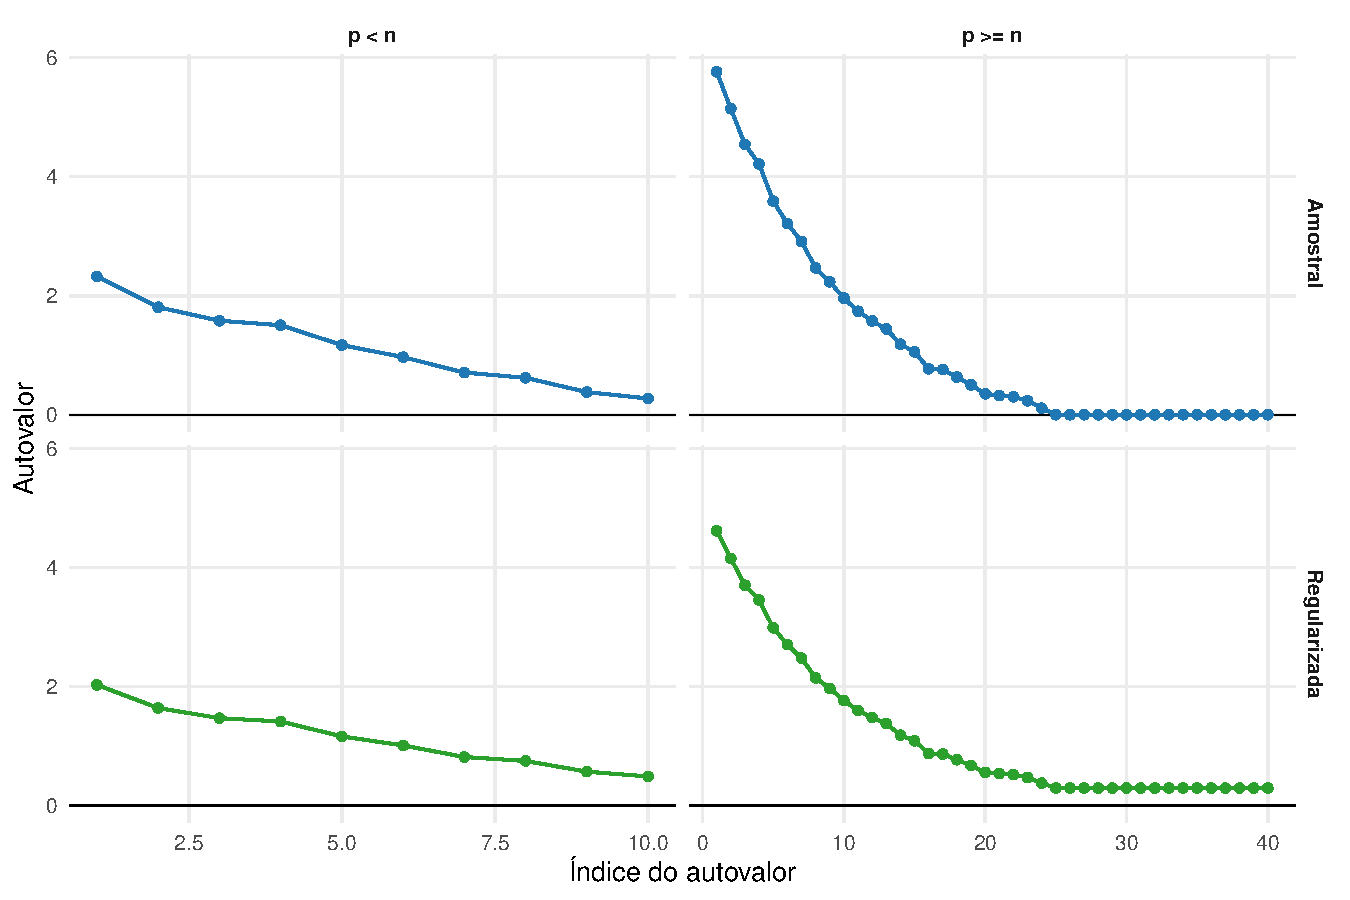
\includegraphics[keepaspectratio]{mod_2_amostrais_files/figure-pdf/fig-espectro-regularizacao-covariancia-1.pdf}}

}

\caption{\label{fig-espectro-regularizacao-covariancia}Espectros da
matriz de covariâncias amostral e de sua versão regularizada em dois
regimes dimensionais.}

\end{figure}%

No regime \(p<n\), a regularização desloca os autovalores na direção do
alvo. No regime \(p\geq n\), os autovalores nulos decorrentes do limite
de posto são substituídos por valores positivos.

A figura mostra um efeito algébrico da regularização. A escolha de
\(\lambda\) e do alvo é um problema estatístico distinto e não será
desenvolvida algoritmicamente neste capítulo.

\subsection{Pseudoinversa e
regularização}\label{pseudoinversa-e-regularizauxe7uxe3o}

A pseudoinversa de Moore--Penrose foi definida na
Definição~\ref{def-pseudoinversa-svd}. Para uma matriz de covariâncias
amostral com decomposição espectral reduzida

\[
\mathbf S
=
\mathbf Q_r
\boldsymbol{\Lambda}_r
\mathbf Q_r^\top,
\]

em que \(\boldsymbol{\Lambda}_r\) contém os \(r\) autovalores positivos,
tem-se

\begin{equation}\phantomsection\label{eq-pseudoinversa-covariancia-amostral}{
\mathbf S^+
=
\mathbf Q_r
\boldsymbol{\Lambda}_r^{-1}
\mathbf Q_r^\top.
}\end{equation}

A pseudoinversa e a regularização resolvem problemas matemáticos
diferentes.

Para visualizar essa diferença, considere

\[
\mathbf S
=
\mathbf Q
\operatorname{diag}
\left(
\ell_1,\ldots,\ell_p
\right)
\mathbf Q^\top,
\]

com

\[
\ell_j\geq0.
\]

A pseudoinversa atribui os pesos

\[
\begin{cases}
1/\ell_j, & \ell_j>0,\\
0, & \ell_j=0.
\end{cases}
\]

Considere agora

\[
\mathbf S_\lambda
=
(1-\lambda)\mathbf S
+
\lambda\tau\mathbf I_p,
\]

com

\[
0<\lambda\leq1
\qquad
\text{e}
\qquad
\tau>0.
\]

Sua inversa é

\begin{equation}\phantomsection\label{eq-inversa-covariancia-regularizada}{
\mathbf S_\lambda^{-1}
=
\mathbf Q
\operatorname{diag}
\left[
\frac{1}{
(1-\lambda)\ell_j+\lambda\tau
}
\right]
\mathbf Q^\top.
}\end{equation}

Se

\[
\ell_j=0,
\]

a pseudoinversa atribui peso zero, enquanto a inversa regularizada
atribui

\[
\frac{1}{\lambda\tau}.
\]

A pseudoinversa não modifica \(\mathbf S\); ela substitui a inversão
usual por sua extensão de Moore--Penrose. Os autovalores positivos
continuam recebendo pesos \(1/\ell_j\), mesmo quando são muito pequenos,
enquanto as direções associadas a autovalores nulos recebem peso zero.

A regularização modifica a própria matriz utilizada para estimar
\(\boldsymbol{\Sigma}\) e define outro procedimento estatístico. Na
contração esférica, os autovalores são afastados de zero e a inversão
passa a utilizar pesos finitos determinados pelos autovalores
regularizados. Portanto, pseudoinversa e regularização tratam a
singularidade por mecanismos diferentes.

\begin{tcolorbox}[enhanced jigsaw, colback=white, breakable, bottomrule=.15mm, left=2mm, arc=.35mm, rightrule=.15mm, colframe=quarto-callout-caution-color-frame, toprule=.15mm, leftrule=.75mm, opacityback=0]

\vspace{-3mm}\textbf{Invertibilidade não implica validade inferencial}\vspace{3mm}

Substituir \(\mathbf S^{-1}\) por \(\mathbf S^+\) ou por uma inversa
regularizada modifica a estatística utilizada.

Distribuições amostrais e calibrações inferenciais derivadas para a
inversa clássica não podem ser transferidas automaticamente para essas
substituições.

\end{tcolorbox}

\subsection{Sensibilidade e robustez}\label{sensibilidade-e-robustez}

O vetor de médias e a matriz de covariâncias amostrais podem sofrer
alterações arbitrariamente grandes quando uma observação é substituída
por outra suficientemente afastada da maior parte dos dados (Maronna et
al., 2019).

Considere a substituição de uma observação \(\mathbf x_k\) por
\(\mathbf x_k^\ast\). A nova média é

\begin{equation}\phantomsection\label{eq-efeito-substituicao-media}{
\bar{\mathbf x}^{\ast}
=
\bar{\mathbf x}
+
\frac{1}{n}
\left(
\mathbf x_k^\ast-\mathbf x_k
\right).
}\end{equation}

Portanto,

\[
\bar{\mathbf x}^{\ast}
-
\bar{\mathbf x}
=
\frac{1}{n}
\left(
\mathbf x_k^\ast-\mathbf x_k
\right).
\]

A alteração não possui limite uniforme quando \(\mathbf x_k^\ast\) pode
se afastar arbitrariamente dos demais dados. Assim, uma única observação
pode produzir uma mudança arbitrariamente grande na média amostral.

Na matriz de covariâncias, os produtos externos

\[
\left(
\mathbf x_i-\bar{\mathbf x}
\right)
\left(
\mathbf x_i-\bar{\mathbf x}
\right)^\top
\]

fazem com que observações afastadas possam modificar simultaneamente
dispersões, covariâncias e direções espectrais.

Uma observação extrema não deve ser identificada automaticamente como
erro. Ela pode representar uma unidade válida situada em uma região
pouco frequente da população, uma observação proveniente de outra
população ou um erro de registro ou medição. O comportamento extremo
também pode indicar que a distribuição possui caudas mais pesadas,
assimetria ou heterogeneidade não representadas pelo modelo adotado.

A decisão de manter, corrigir ou excluir uma observação exige
conhecimento do processo de coleta e do contexto.

Estimadores robustos de localização e dispersão procuram limitar
determinados tipos de sensibilidade. Sua comparação depende de quanto as
estimativas se alteram diante de observações contaminadas, da eficiência
sob o modelo adotado como referência, da equivariância, das condições de
existência em função de \(n\) e \(p\), do custo computacional e do
parâmetro de localização ou dispersão que o procedimento pretende
estimar. Nenhum procedimento apresenta o melhor desempenho em todos
esses critérios.

Observações extremas, alta dimensão e má especificação correspondem a
problemas diferentes. Observações extremas podem alterar fortemente
estimadores sensíveis. A alta dimensão afeta o número de parâmetros a
estimar, o posto e a estabilidade da matriz. A má especificação ocorre
quando a distribuição ou a estrutura assumida pelo modelo não representa
adequadamente o processo que gerou os dados. Esses problemas podem
ocorrer simultaneamente, mas exigem tratamentos diferentes.

A avaliação de uma matriz de covariâncias estimada depende da finalidade
da análise. Tamanho amostral e dimensão determinam restrições de posto;
o espectro informa sobre direções de variabilidade e condicionamento; as
escalas das variáveis influenciam a interpretação e a escolha de alvos
de regularização; e a sensibilidade das estimativas deve ser considerada
quando observações extremas ou desvios do modelo podem alterar
substancialmente os resultados.

O exemplo integrado a seguir reúne os principais objetos construídos no
capítulo em uma única amostra.

\section{Exemplo integrado}\label{exemplo-integrado}

O exemplo reúne a estimação da localização, da dispersão e das relações
entre dois blocos de variáveis. Como os cálculos são realizados para uma
amostra observada, os resultados numéricos são estimativas,
representadas pelos correspondentes objetos observados.

\begin{example}[Estimação em dois blocos de
variáveis]\protect\hypertarget{exm-estimacao-integrada}{}\label{exm-estimacao-integrada}

Considere seis unidades amostrais nas quais foram observados dois blocos
de variáveis. O primeiro bloco contém três variáveis:

\[
\mathbf X
=
\begin{bmatrix}
2 & 4 & 2\\
3 & 5 & 3\\
3 & 6 & 3\\
5 & 7 & 4\\
5 & 6 & 6\\
6 & 8 & 6
\end{bmatrix}
\in
\mathbb R^{6\times3}.
\]

O segundo bloco contém duas variáveis observadas nas mesmas unidades:

\[
\mathbf Y
=
\begin{bmatrix}
1 & 3\\
3 & 2\\
4 & 5\\
5 & 7\\
3 & 4\\
8 & 9
\end{bmatrix}
\in
\mathbb R^{6\times2}.
\]

A correspondência entre as linhas de \(\mathbf X\) e \(\mathbf Y\)
precisa ser preservada para a estimação das covariâncias cruzadas.

Os valores foram escolhidos para que as médias sejam inteiras e os
produtos cruzados possam ser calculados sem arredondamento. Os vetores
de médias observados são

\[
\bar{\mathbf x}
=
\frac{1}{6}
\mathbf X^\top
\mathbf 1_6
=
\begin{bmatrix}
4\\
6\\
4
\end{bmatrix}
\]

e

\[
\bar{\mathbf y}
=
\frac{1}{6}
\mathbf Y^\top
\mathbf 1_6
=
\begin{bmatrix}
4\\
5
\end{bmatrix}.
\]

As matrizes centralizadas são, portanto,

\[
\mathbf X_c
=
\begin{bmatrix}
-2 & -2 & -2\\
-1 & -1 & -1\\
-1 & 0 & -1\\
1 & 1 & 0\\
1 & 0 & 2\\
2 & 2 & 2
\end{bmatrix}
\]

e

\[
\mathbf Y_c
=
\begin{bmatrix}
-3 & -2\\
-1 & -3\\
0 & 0\\
1 & 2\\
-1 & -1\\
4 & 4
\end{bmatrix}.
\]

Em ambas as matrizes, cada coluna soma zero, como exige a centralização
pela média amostral.

Para o primeiro bloco, a matriz SQPC observada é

\[
\mathbf T_X
=
\mathbf X_c^\top
\mathbf X_c.
\]

Os elementos da diagonal são somas de quadrados. Por exemplo,

\[
t_{11}
=
(-2)^2+(-1)^2+(-1)^2+1^2+1^2+2^2
=
12.
\]

Os elementos fora da diagonal são somas de produtos cruzados. Por
exemplo,

\[
\begin{aligned}
t_{12}
&=
(-2)(-2)
+
(-1)(-1)
+
(-1)(0)
+
(1)(1)
+
(1)(0)
+
(2)(2)
\\
&=
10.
\end{aligned}
\]

Calculando os demais elementos da mesma forma,

\begin{equation}\phantomsection\label{eq-exemplo-sqpc-primeiro-bloco}{
\mathbf T_X
=
\begin{bmatrix}
12 & 10 & 12\\
10 & 10 & 9\\
12 & 9 & 14
\end{bmatrix}.
}\end{equation}

A simetria decorre de \(t_{jk}=t_{kj}\), de modo que somente a diagonal
e uma das partes triangulares precisam ser calculadas diretamente.

A matriz de covariâncias amostral utiliza o divisor

\[
n-1=5.
\]

Logo,

\begin{equation}\phantomsection\label{eq-exemplo-covariancia-primeiro-bloco}{
\begin{aligned}
\mathbf S_X
&=
\frac{1}{5}
\mathbf T_X
\\
&=
\begin{bmatrix}
2,4 & 2,0 & 2,4\\
2,0 & 2,0 & 1,8\\
2,4 & 1,8 & 2,8
\end{bmatrix}.
\end{aligned}
}\end{equation}

A matriz \(\mathbf S_X\) é a realização observada do estimador não
viesado \(\boldsymbol{\mathsf S}_X\) de \(\boldsymbol{\Sigma}_{XX}\),
cujo não viesamento foi estabelecido na
Equação~\ref{eq-nao-viesamento-covariancia-amostral}.

Sob o modelo normal multivariado definido na
Definição~\ref{def-normal-multivariada}, nesta amostra

\[
\operatorname{posto}
\left(
\mathbf T_X
\right)
=
3.
\]

Portanto, a condição de posto completo da
Proposição~\ref{prp-estimadores-normais-mv} é satisfeita. Assim, a
estimativa de máxima verossimilhança da matriz de covariâncias é

\begin{equation}\phantomsection\label{eq-exemplo-mv-covariancia-primeiro-bloco}{
\begin{aligned}
\widehat{\boldsymbol{\Sigma}}_{XX,\mathrm{MV,obs}}
&=
\frac{1}{6}
\mathbf T_X
\\
&=
\begin{bmatrix}
2 & 5/3 & 2\\
5/3 & 5/3 & 3/2\\
2 & 3/2 & 7/3
\end{bmatrix}.
\end{aligned}
}\end{equation}

As duas matrizes estão relacionadas por

\[
\widehat{\boldsymbol{\Sigma}}_{XX,\mathrm{MV,obs}}
=
\frac{5}{6}
\mathbf S_X.
\]

Como diferem apenas pelo fator escalar positivo \(5/6\), possuem os
mesmos autovetores e o mesmo posto. Seus autovalores diferem pelo fator
\(5/6\), enquanto o número de condição espectral permanece inalterado.

Em cálculos manuais, os valores exatos devem ser mantidos enquanto
possível. Por isso, a estimativa de máxima verossimilhança foi
apresentada em forma fracionária. O arredondamento deve ser realizado
apenas na apresentação dos resultados que não admitem uma representação
exata simples. Utilizar valores já arredondados de médias, covariâncias,
correlações ou autovalores em cálculos posteriores pode acumular erros e
produzir resultados diferentes dos obtidos a partir dos valores exatos.

Neste exemplo, \(\mathbf T_X\) é exata e \(\mathbf S_X=\mathbf T_X/5\)
possui representação decimal finita. Para calcular correlações, pode-se
utilizar diretamente

\[
r_{jk}
=
\frac{t_{jk}}
{\sqrt{t_{jj}t_{kk}}},
\]

pois o divisor comum de \(\mathbf S_X\) se cancela. Autovalores e
números de condição apresentados em forma decimal devem ser calculados
com os valores não arredondados e arredondados apenas ao final.

A matriz de correlações observada é

\begin{equation}\phantomsection\label{eq-exemplo-correlacao-primeiro-bloco}{
\mathbf R_X
\approx
\begin{bmatrix}
1,000 & 0,913 & 0,926\\
0,913 & 1,000 & 0,761\\
0,926 & 0,761 & 1,000
\end{bmatrix}.
}\end{equation}

As três correlações são positivas. A maior ocorre entre \(X_1\) e
\(X_3\),

\[
r_{13}
\approx
0,926,
\]

e a menor entre \(X_2\) e \(X_3\),

\[
r_{23}
\approx
0,761.
\]

Os autovalores de \(\mathbf S_X\), em ordem decrescente, são
aproximadamente

\[
\ell_1
\approx
6,579,
\qquad
\ell_2
\approx
0,560
\qquad
\text{e}
\qquad
\ell_3
\approx
0,061.
\]

Como todos são positivos,

\[
\operatorname{posto}
\left(
\mathbf S_X
\right)
=
3,
\]

e

\[
\mathbf S_X
\succ
\mathbf0.
\]

Seu número de condição espectral é aproximadamente

\[
\kappa_2
\left(
\mathbf S_X
\right)
=
\frac{\ell_1}{\ell_3}
\approx
108,3.
\]

O valor de \(\kappa_2(\mathbf S_X)\) foi calculado com os autovalores
antes do arredondamento. Dividir os valores exibidos, já arredondados,
pode produzir uma aproximação ligeiramente diferente.

Portanto, \(\mathbf S_X\) é invertível, mas seus autovalores apresentam
magnitudes bastante distintas. O valor relativamente elevado de
\(\kappa_2(\mathbf S_X)\) mostra que invertibilidade e bom
condicionamento são propriedades distintas.

Para estimar as relações entre os dois blocos, utiliza-se

\[
\mathbf T_{XY}
=
\mathbf X_c^\top
\mathbf Y_c.
\]

Por exemplo, o elemento correspondente a \(X_1\) e \(Y_1\) é

\[
\begin{aligned}
t_{X_1Y_1}
&=
(-2)(-3)
+
(-1)(-1)
+
(-1)(0)
+
(1)(1)
+
(1)(-1)
+
(2)(4)
\\
&=
15.
\end{aligned}
\]

Os demais produtos cruzados fornecem

\begin{equation}\phantomsection\label{eq-exemplo-sscp-cruzada}{
\mathbf T_{XY}
=
\begin{bmatrix}
15 & 16\\
16 & 17\\
13 & 13
\end{bmatrix}.
}\end{equation}

Logo, pela definição de covariância cruzada observada na
Definição~\ref{def-covariancia-cruzada-observada},

\begin{equation}\phantomsection\label{eq-exemplo-covariancia-cruzada}{
\mathbf S_{XY}
=
\frac{1}{5}
\mathbf T_{XY}
=
\begin{bmatrix}
3,0 & 3,2\\
3,2 & 3,4\\
2,6 & 2,6
\end{bmatrix}.
}\end{equation}

Por exemplo,

\[
s_{X_3Y_1}
=
2,6
\]

é a covariância amostral entre \(X_3\) e \(Y_1\).

A inversão da ordem dos blocos segue
Equação~\ref{eq-transposta-covariancia-cruzada-observada}:

\[
\mathbf S_{YX}
=
\mathbf S_{XY}^{\top}
=
\begin{bmatrix}
3,0 & 3,2 & 2,6\\
3,2 & 3,4 & 2,6
\end{bmatrix}.
\]

Para o segundo bloco,

\[
\mathbf T_Y
=
\mathbf Y_c^\top
\mathbf Y_c
=
\begin{bmatrix}
28 & 28\\
28 & 34
\end{bmatrix},
\]

de modo que

\[
\mathbf S_Y
=
\frac{1}{5}
\mathbf T_Y
=
\begin{bmatrix}
5,6 & 5,6\\
5,6 & 6,8
\end{bmatrix}.
\]

Reunindo as cinco variáveis,

\[
\mathbf X_{\mathrm{conj}}
=
\begin{bmatrix}
\mathbf X & \mathbf Y
\end{bmatrix}
\in
\mathbb R^{6\times5},
\]

a matriz SQPC conjunta possui a forma em blocos

\[
\mathbf T_{\mathrm{conj}}
=
\begin{bmatrix}
\mathbf T_X
&
\mathbf T_{XY}
\\
\mathbf T_{YX}
&
\mathbf T_Y
\end{bmatrix}.
\]

Numericamente,

\[
\mathbf T_{\mathrm{conj}}
=
\begin{bmatrix}
12 & 10 & 12 & 15 & 16\\
10 & 10 & 9 & 16 & 17\\
12 & 9 & 14 & 13 & 13\\
15 & 16 & 13 & 28 & 28\\
16 & 17 & 13 & 28 & 34
\end{bmatrix}.
\]

Como \(n-1=5\),

\begin{equation}\phantomsection\label{eq-exemplo-covariancia-conjunta}{
\mathbf S_{\mathrm{conj}}
=
\frac{1}{5}
\mathbf T_{\mathrm{conj}}
=
\begin{bmatrix}
2,4 & 2,0 & 2,4 & 3,0 & 3,2\\
2,0 & 2,0 & 1,8 & 3,2 & 3,4\\
2,4 & 1,8 & 2,8 & 2,6 & 2,6\\
3,0 & 3,2 & 2,6 & 5,6 & 5,6\\
3,2 & 3,4 & 2,6 & 5,6 & 6,8
\end{bmatrix}.
}\end{equation}

A organização em blocos permite identificar diretamente as covariâncias
internas de \(\mathbf X\), as covariâncias internas de \(\mathbf Y\) e
as covariâncias cruzadas entre os dois conjuntos.

Como existem seis observações e cinco variáveis,

\[
\operatorname{posto}
\left(
\mathbf S_{\mathrm{conj}}
\right)
\leq
5.
\]

A matriz conjunta centralizada é

\[
\mathbf X_{\mathrm{conj},c}
=
\begin{bmatrix}
-2 & -2 & -2 & -3 & -2\\
-1 & -1 & -1 & -1 & -3\\
-1 & 0 & -1 & 0 & 0\\
1 & 1 & 0 & 1 & 2\\
1 & 0 & 2 & -1 & -1\\
2 & 2 & 2 & 4 & 4
\end{bmatrix}.
\]

Seu escalonamento fornece cinco pivôs, de modo que

\[
\operatorname{posto}
\left(
\mathbf X_{\mathrm{conj},c}
\right)
=
5.
\]

Como

\[
\mathbf T_{\mathrm{conj}}
=
\mathbf X_{\mathrm{conj},c}^{\top}
\mathbf X_{\mathrm{conj},c},
\]

segue de Equação~\ref{eq-posto-sscp-total} que

\[
\operatorname{posto}
\left(
\mathbf S_{\mathrm{conj}}
\right)
=
5.
\]

Portanto,

\[
\mathbf S_{\mathrm{conj}}
\succ
\mathbf0.
\]

O caso \(n=6\) e \(p=5\) está exatamente no limite \(n=p+1\). Esse
tamanho amostral permite posto completo, mas não o garante para uma
amostra arbitrária.

O exemplo mostra como uma única amostra produz realizações dos
principais objetos definidos no capítulo. Os vetores \(\bar{\mathbf x}\)
e \(\bar{\mathbf y}\) estimam as médias populacionais, enquanto
\(\mathbf T_X\) é a realização da estatística SQPC. A divisão de
\(\mathbf T_X\) por \(n-1\) produz a estimativa não viesada
\(\mathbf S_X\); a divisão por \(n\) produz a estimativa pelo método dos
momentos e, sob o modelo normal e as condições de existência do máximo,
também a estimativa de máxima verossimilhança.

A matriz \(\mathbf R_X\) utiliza a mesma informação de covariância após
a remoção das escalas marginais. O posto completo de \(\mathbf S_X\)
garante sua invertibilidade, mas o número de condição mostra que essa
propriedade não garante estabilidade da inversão.

O pareamento das linhas de \(\mathbf X\) e \(\mathbf Y\) determina os
produtos cruzados em \(\mathbf T_{XY}\) e, consequentemente, as
covariâncias em \(\mathbf S_{XY}\). A matriz conjunta reúne em um único
objeto as covariâncias internas dos dois blocos e as covariâncias entre
eles.

Todos os valores apresentados são realizações obtidas nesta amostra. Não
viesamento, consistência, eficiência e outras propriedades dos
estimadores descrevem seu comportamento ao considerar as possíveis
amostras geradas pelo modelo.

\end{example}

\section{Síntese do capítulo}\label{suxedntese-do-capuxedtulo-9}

Este capítulo estabeleceu a relação entre parâmetros populacionais,
estatísticas amostrais, estimadores e suas realizações observadas.

A distinção central envolve quatro objetos. O parâmetro
\(\boldsymbol{\theta}\) é uma característica fixa da distribuição
populacional. Uma amostra aleatória \(\boldsymbol{\mathcal X}\) produz
estatísticas por meio de funções dos dados,

\[
\boldsymbol{\mathsf G}
=
G
\left(
\boldsymbol{\mathcal X}
\right).
\]

Quando uma estatística é utilizada para estimar \(\boldsymbol{\theta}\),
ela constitui um estimador,

\[
\widehat{\boldsymbol{\theta}}
=
G
\left(
\boldsymbol{\mathcal X}
\right).
\]

Após a observação da amostra, a realização

\[
\widehat{\boldsymbol{\theta}}_{\mathrm{obs}}
=
G
\left(
\mathbf X
\right)
\]

é a estimativa do parâmetro. Portanto, todo estimador é uma estatística,
mas nem toda estatística é utilizada como estimador.

Para uma amostra multivariada i.i.d., o vetor de médias amostrais estima
\(\boldsymbol{\mu}\), enquanto a matriz de covariâncias amostral estima
\(\boldsymbol{\Sigma}\):

\[
\bar{\boldsymbol{\mathsf X}}
=
\frac{1}{n}
\sum_{i=1}^{n}
\boldsymbol{\mathsf X}_i
\]

e

\[
\boldsymbol{\mathsf S}
=
\frac{1}{n-1}
\boldsymbol{\mathsf T},
\]

em que \(\boldsymbol{\mathsf T}\) é a matriz SQPC amostral definida na
Definição~\ref{def-sscp-amostral-aleatoria}.

O método dos momentos e a máxima verossimilhança são princípios de
construção de estimadores. O método utilizado não determina, por si só,
as propriedades do estimador obtido.

O método dos momentos fornece

\[
\widehat{\boldsymbol{\mu}}_{\mathrm{MM}}
=
\bar{\boldsymbol{\mathsf X}}
\]

e

\[
\widehat{\boldsymbol{\Sigma}}_{\mathrm{MM}}
=
\frac{1}{n}
\boldsymbol{\mathsf T}.
\]

Sob o modelo normal multivariado e quando o máximo existe, a máxima
verossimilhança conduz às mesmas estatísticas.

A segunda estatística é viesada em amostras finitas, enquanto

\[
\boldsymbol{\mathsf S}
=
\frac{1}{n-1}
\boldsymbol{\mathsf T}
\]

é não viesada. As duas são consistentes para \(\boldsymbol{\Sigma}\) no
regime de dimensão fixa sob as condições estabelecidas no capítulo.

Os resultados na Proposição~\ref{prp-media-amostral-momentos} e
Equação~\ref{eq-nao-viesamento-covariancia-amostral} fornecem

\[
E
\left(
\bar{\boldsymbol{\mathsf X}}
\right)
=
\boldsymbol{\mu},
\qquad
\operatorname{Cov}
\left(
\bar{\boldsymbol{\mathsf X}}
\right)
=
\frac{\boldsymbol{\Sigma}}{n},
\qquad
E
\left(
\boldsymbol{\mathsf S}
\right)
=
\boldsymbol{\Sigma}.
\]

No regime de dimensão fixa,
Proposição~\ref{prp-consistencia-media-amostral} e
Proposição~\ref{prp-consistencia-covariancia-amostral} estabelecem

\[
\bar{\boldsymbol{\mathsf X}}
\xrightarrow{P}
\boldsymbol{\mu}
\qquad
\text{e}
\qquad
\boldsymbol{\mathsf S}
\xrightarrow{P}
\boldsymbol{\Sigma}.
\]

Para variáveis organizadas em dois blocos pareados,

\[
\boldsymbol{\mathsf S}_{XY}
=
\frac{1}{n-1}
\boldsymbol{\mathsf T}_{XY}
\]

estima a matriz de covariâncias cruzadas. Quando as variâncias amostrais
são positivas,

\[
\boldsymbol{\mathsf R}
=
\boldsymbol{\mathsf D}_S^{-1/2}
\boldsymbol{\mathsf S}
\boldsymbol{\mathsf D}_S^{-1/2}
\]

fornece a matriz de correlações amostral.

A Tabela~\ref{tbl-sintese-estimacao-amostral} reúne os principais
objetos do capítulo.

\begin{longtable}[]{@{}
  >{\raggedright\arraybackslash}p{(\linewidth - 6\tabcolsep) * \real{0.2500}}
  >{\raggedright\arraybackslash}p{(\linewidth - 6\tabcolsep) * \real{0.2500}}
  >{\raggedright\arraybackslash}p{(\linewidth - 6\tabcolsep) * \real{0.2500}}
  >{\raggedright\arraybackslash}p{(\linewidth - 6\tabcolsep) * \real{0.2500}}@{}}
\caption{Relação entre parâmetros, estatísticas, estimadores e valores
observados utilizados no
capítulo.}\label{tbl-sintese-estimacao-amostral}\tabularnewline
\toprule\noalign{}
\begin{minipage}[b]{\linewidth}\raggedright
Parâmetro ou objeto
\end{minipage} & \begin{minipage}[b]{\linewidth}\raggedright
Estatística/estimador
\end{minipage} & \begin{minipage}[b]{\linewidth}\raggedright
Propriedade destacada
\end{minipage} & \begin{minipage}[b]{\linewidth}\raggedright
Valor observado
\end{minipage} \\
\midrule\noalign{}
\endfirsthead
\toprule\noalign{}
\begin{minipage}[b]{\linewidth}\raggedright
Parâmetro ou objeto
\end{minipage} & \begin{minipage}[b]{\linewidth}\raggedright
Estatística/estimador
\end{minipage} & \begin{minipage}[b]{\linewidth}\raggedright
Propriedade destacada
\end{minipage} & \begin{minipage}[b]{\linewidth}\raggedright
Valor observado
\end{minipage} \\
\midrule\noalign{}
\endhead
\bottomrule\noalign{}
\endlastfoot
\(\boldsymbol{\mu}\) & \(\bar{\boldsymbol{\mathsf X}}\) & Não viesado e
consistente; MM; MV sob normalidade e existência do máximo &
\(\bar{\mathbf x}\) \\
\(\boldsymbol{\Sigma}\) &
\(\boldsymbol{\mathsf S}=\boldsymbol{\mathsf T}/(n-1)\) & Não viesado e
consistente & \(\mathbf S\) \\
\(\boldsymbol{\Sigma}\) & \(\boldsymbol{\mathsf T}/n\) & MM; MV sob
normalidade e existência do máximo; viesado em amostras finitas e
consistente & \(\mathbf T/n\) \\
SQPC amostral & \(\boldsymbol{\mathsf T}\) & Estatística que reúne somas
de quadrados e produtos cruzados & \(\mathbf T\) \\
\(\boldsymbol{\Sigma}_{XY}\) & \(\boldsymbol{\mathsf S}_{XY}\) & Não
viesado e consistente & \(\mathbf S_{XY}\) \\
\(\boldsymbol{\mathcal R}\) & \(\boldsymbol{\mathsf R}\) & Em geral
viesado, mas consistente; MV sob normalidade e existência do máximo &
\(\mathbf R\) \\
\end{longtable}

As propriedades estudadas respondem a perguntas diferentes. O viés
compara a esperança do estimador com o parâmetro; a variabilidade
descreve quanto o estimador muda entre amostras; o erro quadrático médio
combina erro sistemático e variabilidade segundo uma função de perda; a
consistência descreve o comportamento quando \(n\) aumenta; e a
eficiência compara estimadores concorrentes segundo sua variabilidade ou
risco. A suficiência verifica se uma redução da amostra preserva a
informação sobre o parâmetro, enquanto a equivariância descreve a
resposta do estimador a transformações dos dados. A robustez examina
quanto o procedimento pode ser alterado pelas formas de contaminação ou
perturbação consideradas.

A estrutura de posto

\[
\operatorname{posto}
\left(
\boldsymbol{\mathsf S}
\right)
\leq
\min
\left(
p,n-1
\right)
\]

mostra por que dimensão e tamanho amostral precisam ser considerados
conjuntamente. Quando \(p\geq n\), a covariância amostral é
necessariamente singular. Mesmo quando existe uma inversa, seu uso pode
ser instável quando alguns autovalores são pequenos.

Pseudoinversa e regularização tratam singularidade e condicionamento por
mecanismos diferentes. A pseudoinversa mantém \(\mathbf S\) e modifica a
operação utilizada para trabalhar com suas direções de variância nula. A
regularização substitui \(\mathbf S\) por outro estimador, por exemplo
combinando-a com uma matriz-alvo. Essa modificação pode afastar
autovalores de zero e melhorar o condicionamento, mas também altera
viés, risco e consistência. Com peso de contração fixo e alvo diferente
de \(\boldsymbol{\Sigma}\), a consistência para \(\boldsymbol{\Sigma}\)
não é garantida.

Ao término deste capítulo, deve-se ser capaz de:

\begin{itemize}
\tightlist
\item
  distinguir parâmetro, estatística, estimador, estimativa e
  distribuição amostral;
\item
  avaliar viés, variabilidade, erro quadrático médio, consistência,
  eficiência, suficiência, equivariância e robustez;
\item
  distinguir os princípios do método dos momentos e da máxima
  verossimilhança;
\item
  construir o vetor de médias amostrais, a matriz SQPC e os estimadores
  da matriz de covariâncias;
\item
  explicar a origem e a função dos divisores \(n\) e \(n-1\);
\item
  construir estimadores de covariâncias cruzadas e correlações;
\item
  analisar posto, singularidade e condicionamento de matrizes estimadas;
\item
  distinguir pseudoinversa, regularização e estimação robusta segundo o
  problema que cada procedimento procura tratar.
\end{itemize}

O Capítulo 11 utiliza a matriz de covariâncias populacional de
Definição~\ref{def-matriz-covariancias-populacional}, o modelo normal
multivariado de Definição~\ref{def-normal-multivariada} e os estimadores
desenvolvidos neste capítulo para construir o \textbf{modelo linear
multivariado}. Nesse modelo, várias variáveis-resposta são relacionadas
simultaneamente a uma matriz de delineamento, produzindo uma matriz de
parâmetros, valores ajustados, resíduos e matrizes SQPC associadas às
fontes de variação.

\chapter{Modelo Linear Multivariado e Hipóteses
Lineares}\label{modelo-linear-multivariado-e-hipuxf3teses-lineares}

O Capítulo 10 desenvolveu a estimação do vetor de médias e da matriz de
covariâncias a partir de uma amostra aleatória multivariada. O vetor de
médias amostrais e suas propriedades foram estabelecidos em
Proposição~\ref{prp-media-amostral-momentos}, enquanto a matriz de
covariâncias amostral foi definida em
Definição~\ref{def-matriz-covariancias-amostral-aleatoria} e seu não
viesamento foi estabelecido em
Proposição~\ref{prp-nao-viesamento-covariancia-amostral}. Nesse
contexto, todas as unidades compartilhavam o mesmo vetor de médias
populacional.

O modelo linear multivariado substitui essa média comum por uma
estrutura de médias que pode variar entre as unidades segundo
características conhecidas. Essa formulação permite representar, em um
mesmo modelo, regressões com várias respostas, comparações entre grupos,
efeitos de fatores e efeitos de covariáveis.

O modelo é escrito como

\[
\boldsymbol{\mathcal Y}
=
\mathbf Z\mathbf B
+
\boldsymbol{\mathcal E},
\]

em que:

\begin{itemize}
\tightlist
\item
  \(\boldsymbol{\mathcal Y}\in\mathbb R^{n\times p}\) é a matriz
  aleatória de respostas;
\item
  \(\mathbf Z\in\mathbb R^{n\times q}\) é a matriz de delineamento;
\item
  \(\mathbf B\in\mathbb R^{q\times p}\) é a matriz de parâmetros;
\item
  \(\boldsymbol{\mathcal E}\in\mathbb R^{n\times p}\) é a matriz
  aleatória de erros.
\end{itemize}

Aqui, \(n\) é o número de unidades, \(p\) é o número de respostas
observadas em cada unidade e \(q\) é o número de termos representados na
matriz de delineamento. Esses termos podem incluir intercepto,
indicadores de grupos ou tratamentos e covariáveis quantitativas.

O objetivo deste capítulo é formular o modelo, estimar \(\mathbf B\),
interpretar valores ajustados e resíduos por meio de projeções,
construir a SQPC residual, estimar a matriz de covariâncias dos erros,
decompor a dispersão observada e representar hipóteses lineares sobre
parâmetros e combinações das respostas (Rencher; Christensen, 2012).

No caso de grupos, essa estrutura relacionará a variação residual e a
variação associada ao modelo às matrizes de dispersão intragrupos e
entre grupos definidas em Definição~\ref{def-sscp-intragrupos} e
Definição~\ref{def-sscp-entre-grupos}.

As distribuições amostrais utilizadas na construção de testes e regiões
de confiança serão desenvolvidas no Capítulo 12.

\begin{tcolorbox}[enhanced jigsaw, colback=white, breakable, bottomrule=.15mm, left=2mm, arc=.35mm, rightrule=.15mm, colframe=quarto-callout-note-color-frame, toprule=.15mm, leftrule=.75mm, opacityback=0]

\vspace{-3mm}\textbf{Convenções de notação}\vspace{3mm}

Ao longo deste capítulo:

\begin{itemize}
\tightlist
\item
  \(\boldsymbol{\mathsf Y}_i\in\mathbb R^p\) representa o vetor
  aleatório de respostas da unidade \(i\);
\item
  \(\mathbf y_i\in\mathbb R^p\) representa uma realização desse vetor;
\item
  \(\boldsymbol{\mathcal Y}\in\mathbb R^{n\times p}\) representa a
  matriz aleatória de respostas;
\item
  \(\mathbf Y\in\mathbb R^{n\times p}\) representa a matriz observada de
  respostas;
\item
  \(\mathbf Z\in\mathbb R^{n\times q}\) representa a matriz de
  delineamento;
\item
  \(\mathbf z_i^\top\) representa a linha \(i\) de \(\mathbf Z\);
\item
  \(\mathbf B\in\mathbb R^{q\times p}\) representa a matriz de
  parâmetros;
\item
  \(\boldsymbol{\varepsilon}_i\in\mathbb R^p\) representa o vetor
  aleatório de erros da unidade \(i\);
\item
  \(\boldsymbol{\mathcal E}\in\mathbb R^{n\times p}\) representa a
  matriz aleatória de erros;
\item
  \(\boldsymbol{\Sigma}\in\mathbb R^{p\times p}\) representa a matriz de
  covariâncias entre as respostas de uma mesma unidade;
\item
  \(\widehat{\mathbf B}\) representa um estimador de \(\mathbf B\);
\item
  \(\widehat{\boldsymbol{\mathcal U}}\) representará a matriz aleatória
  de resíduos e \(\widehat{\mathbf U}\) sua realização observada;
\item
  \(\boldsymbol{\mathsf E}_{\mathrm{res}}\) representará a SQPC residual
  como estatística aleatória e \(\mathbf E\) sua realização observada;
\item
  \(\mathbf T\) continuará representando a SQPC total observada;
\item
  \(\mathbf T_{\mathrm{mod}}\) representará a dispersão dos valores
  ajustados pelo modelo em torno da média geral;
\item
  \(\mathbf H\) ficará reservada à SQPC associada a uma hipótese linear.
\end{itemize}

A letra \(\mathbf Z\) é utilizada para o delineamento para preservar
\(\mathbf X\) como símbolo da matriz de dados nos capítulos anteriores.

\end{tcolorbox}

\section{Formulação do modelo linear
multivariado}\label{formulauxe7uxe3o-do-modelo-linear-multivariado}

\subsection{Resposta vetorial e matriz de
respostas}\label{resposta-vetorial-e-matriz-de-respostas}

No modelo linear univariado, cada unidade fornece uma única resposta. No
caso multivariado, a unidade \(i\) fornece simultaneamente

\begin{equation}\phantomsection\label{eq-vetor-respostas-unidade}{
\boldsymbol{\mathsf Y}_i
=
\begin{bmatrix}
Y_{i1}\\
Y_{i2}\\
\vdots\\
Y_{ip}
\end{bmatrix}
\in
\mathbb R^p.
}\end{equation}

As componentes podem apresentar dependência. O modelo deve, portanto,
representar simultaneamente:

\begin{enumerate}
\def\labelenumi{\arabic{enumi}.}
\tightlist
\item
  a estrutura das médias das \(p\) respostas;
\item
  a variabilidade de cada resposta;
\item
  as covariâncias entre respostas observadas na mesma unidade.
\end{enumerate}

Considere

\[
\mathbf z_i
=
\begin{bmatrix}
z_{i1}\\
\vdots\\
z_{iq}
\end{bmatrix}
\in
\mathbb R^q,
\]

contendo os valores dos \(q\) termos do modelo para a unidade \(i\).

Um termo pode representar, por exemplo, o intercepto, o pertencimento a
um grupo ou tratamento, o valor de uma covariável quantitativa ou outro
efeito especificado no modelo. A matriz de delineamento reúne essas
informações para todas as unidades.

A matriz de parâmetros é

\begin{equation}\phantomsection\label{eq-matriz-parametros-modelo-multivariado}{
\mathbf B
=
\begin{bmatrix}
\beta_{11} & \beta_{12} & \cdots & \beta_{1p}\\
\beta_{21} & \beta_{22} & \cdots & \beta_{2p}\\
\vdots & \vdots & \ddots & \vdots\\
\beta_{q1} & \beta_{q2} & \cdots & \beta_{qp}
\end{bmatrix}
\in
\mathbb R^{q\times p}.
}\end{equation}

A coluna \(j\) de \(\mathbf B\) contém os coeficientes do modelo para a
resposta \(j\). A linha \(h\) reúne os coeficientes associados ao mesmo
termo da matriz de delineamento para as \(p\) respostas.

Assim, uma covariável ou um efeito de grupo pode atuar de maneira
diferente sobre cada resposta, embora todas utilizem a mesma matriz
\(\mathbf Z\).

A média condicional do vetor de respostas da unidade \(i\) é

\begin{equation}\phantomsection\label{eq-media-condicional-vetor-respostas}{
E
\left(
\boldsymbol{\mathsf Y}_i
\mid
\mathbf Z
\right)
=
\mathbf B^\top
\mathbf z_i.
}\end{equation}

Equivalentemente, em forma de vetor linha,

\[
E
\left(
\boldsymbol{\mathsf Y}_i^\top
\mid
\mathbf Z
\right)
=
\mathbf z_i^\top
\mathbf B.
\]

\begin{definition}[Modelo linear multivariado para uma
unidade]\protect\hypertarget{def-modelo-linear-multivariado-unidade}{}\label{def-modelo-linear-multivariado-unidade}

O vetor de respostas da unidade \(i\) é representado por

\begin{equation}\phantomsection\label{eq-modelo-linear-multivariado-unidade}{
\boldsymbol{\mathsf Y}_i
=
\mathbf B^\top
\mathbf z_i
+
\boldsymbol{\varepsilon}_i,
}\end{equation}

em que

\[
\boldsymbol{\mathsf Y}_i,
\boldsymbol{\varepsilon}_i
\in
\mathbb R^p,
\qquad
\mathbf z_i
\in
\mathbb R^q,
\qquad
\mathbf B
\in
\mathbb R^{q\times p}.
\]

\end{definition}

Componente a componente,

\begin{equation}\phantomsection\label{eq-equacoes-modelo-por-resposta}{
Y_{ij}
=
\mathbf z_i^\top
\boldsymbol{\beta}_j
+
\varepsilon_{ij},
\qquad
j=1,\ldots,p,
}\end{equation}

em que \(\boldsymbol{\beta}_j\) é a coluna \(j\) de \(\mathbf B\).

As equações das diferentes respostas compartilham a mesma matriz de
delineamento. O caráter multivariado do modelo decorre da análise
conjunta dessas respostas e da estrutura de covariâncias dos respectivos
erros.

Para reunir as \(n\) unidades, defina a matriz aleatória

\begin{definition}[Matriz aleatória de
respostas]\protect\hypertarget{def-matriz-aleatoria-respostas}{}\label{def-matriz-aleatoria-respostas}

\begin{equation}\phantomsection\label{eq-matriz-aleatoria-respostas}{
\boldsymbol{\mathcal Y}
=
\begin{bmatrix}
\boldsymbol{\mathsf Y}_1^\top\\
\boldsymbol{\mathsf Y}_2^\top\\
\vdots\\
\boldsymbol{\mathsf Y}_n^\top
\end{bmatrix}
=
\begin{bmatrix}
Y_{11} & \cdots & Y_{1p}\\
Y_{21} & \cdots & Y_{2p}\\
\vdots & \ddots & \vdots\\
Y_{n1} & \cdots & Y_{np}
\end{bmatrix}
\in
\mathbb R^{n\times p}.
}\end{equation}

\end{definition}

Após a observação,

\begin{equation}\phantomsection\label{eq-matriz-observada-respostas}{
\mathbf Y
=
\begin{bmatrix}
\mathbf y_1^\top\\
\vdots\\
\mathbf y_n^\top
\end{bmatrix}
\in
\mathbb R^{n\times p}.
}\end{equation}

A matriz de delineamento é

\begin{equation}\phantomsection\label{eq-matriz-delineamento-modelo-multivariado}{
\mathbf Z
=
\begin{bmatrix}
\mathbf z_1^\top\\
\mathbf z_2^\top\\
\vdots\\
\mathbf z_n^\top
\end{bmatrix}
\in
\mathbb R^{n\times q}.
}\end{equation}

Neste capítulo, o modelo e os resultados de estimação são formulados
condicionalmente a \(\mathbf Z\). Assim, a matriz de delineamento é
tratada como conhecida. Essa convenção abrange tanto delineamentos
fixados previamente quanto análises condicionais aos valores observados
das variáveis explicativas.

\subsection{Estrutura matricial do
modelo}\label{estrutura-matricial-do-modelo}

Organize os vetores de erros nas linhas de

\begin{equation}\phantomsection\label{eq-matriz-aleatoria-erros-modelo}{
\boldsymbol{\mathcal E}
=
\begin{bmatrix}
\boldsymbol{\varepsilon}_1^\top\\
\vdots\\
\boldsymbol{\varepsilon}_n^\top
\end{bmatrix}
\in
\mathbb R^{n\times p}.
}\end{equation}

\begin{definition}[Modelo linear
multivariado]\protect\hypertarget{def-modelo-linear-multivariado}{}\label{def-modelo-linear-multivariado}

O modelo linear multivariado é

\begin{equation}\phantomsection\label{eq-modelo-linear-multivariado}{
\boldsymbol{\mathcal Y}
=
\mathbf Z\mathbf B
+
\boldsymbol{\mathcal E}.
}\end{equation} em que:

\begin{itemize}
\tightlist
\item
  \(\boldsymbol{\mathcal Y}\in\mathbb R^{n\times p}\) é a matriz
  aleatória de respostas;
\item
  \(\mathbf Z\in\mathbb R^{n\times q}\) é a matriz de delineamento;
\item
  \(\mathbf B\in\mathbb R^{q\times p}\) é a matriz de parâmetros;
\item
  \(\boldsymbol{\mathcal E}\in\mathbb R^{n\times p}\) é a matriz
  aleatória de erros.
\end{itemize}

\end{definition}

A matriz de médias condicionais é

\begin{equation}\phantomsection\label{eq-matriz-medias-condicionais-modelo}{
E
\left(
\boldsymbol{\mathcal Y}
\mid
\mathbf Z
\right)
=
\mathbf Z\mathbf B.
}\end{equation}

Portanto, a estrutura sistemática do modelo pertence ao espaço coluna de
\(\mathbf Z\). Cada coluna de

\[
\mathbf Z\mathbf B
\]

é uma combinação linear das colunas do delineamento.

Se

\begin{equation}\phantomsection\label{eq-posto-matriz-delineamento}{
r
=
\operatorname{posto}
\left(
\mathbf Z
\right),
}\end{equation}

então

\[
r\leq\min(n,q).
\]

O valor \(r\) é o número de colunas linearmente independentes de
\(\mathbf Z\) e, portanto, a dimensão do espaço de médias representado
pelo delineamento.

Quando

\[
r=q,
\]

a matriz de delineamento possui posto coluna completo. O caso \(r<q\)
será examinado posteriormente, quando forem discutidas a unicidade dos
coeficientes e as funções estimáveis.

\subsection{Estrutura de médias e covariâncias
residuais}\label{estrutura-de-muxe9dias-e-covariuxe2ncias-residuais}

A primeira condição do modelo é

\begin{definition}[Média residual
nula]\protect\hypertarget{def-hipotese-media-erros-modelo-multivariado}{}\label{def-hipotese-media-erros-modelo-multivariado}

\begin{equation}\phantomsection\label{eq-media-erros-modelo-multivariado}{
E
\left(
\boldsymbol{\varepsilon}_i
\mid
\mathbf Z
\right)
=
\mathbf0,
\qquad
i=1,\ldots,n.
}\end{equation}

\end{definition}

Consequentemente,

\[
E
\left(
\boldsymbol{\mathsf Y}_i
\mid
\mathbf Z
\right)
=
\mathbf B^\top\mathbf z_i.
\]

A segunda condição descreve a dependência entre as respostas de uma
mesma unidade e entre unidades distintas.

\begin{definition}[Estrutura de covariâncias dos
erros]\protect\hypertarget{def-estrutura-covariancia-erros-modelo-multivariado}{}\label{def-estrutura-covariancia-erros-modelo-multivariado}

Para cada unidade,

\[
\boldsymbol{\varepsilon}_i
\in
\mathbb R^p,
\qquad
i=1,\ldots,n,
\]

e assume-se que os segundos momentos condicionais existem.

A matriz de covariâncias condicional é comum às unidades:

\begin{equation}\phantomsection\label{eq-covariancia-comum-erros-modelo}{
\operatorname{Cov}
\left(
\boldsymbol{\varepsilon}_i
\mid
\mathbf Z
\right)
=
\boldsymbol{\Sigma},
\qquad
i=1,\ldots,n,
}\end{equation}

em que

\[
\boldsymbol{\Sigma}
\in
\mathbb R^{p\times p},
\qquad
\boldsymbol{\Sigma}
=
\boldsymbol{\Sigma}^{\top},
\qquad
\boldsymbol{\Sigma}
\succeq
\mathbf0.
\]

Além disso,

\begin{equation}\phantomsection\label{eq-erros-unidades-nao-correlacionados}{
\operatorname{Cov}
\left(
\boldsymbol{\varepsilon}_i,
\boldsymbol{\varepsilon}_\ell
\mid
\mathbf Z
\right)
=
\mathbf0_{p\times p},
\qquad
i\neq\ell.
}\end{equation}

\end{definition}

A matriz

\[
\boldsymbol{\Sigma}
=
\begin{bmatrix}
\sigma_{11} & \cdots & \sigma_{1p}\\
\vdots & \ddots & \vdots\\
\sigma_{p1} & \cdots & \sigma_{pp}
\end{bmatrix}
\]

é a matriz de covariâncias residuais entre as \(p\) respostas.

Assim,

\[
\operatorname{Var}
\left(
Y_{ij}
\mid
\mathbf Z
\right)
=
\sigma_{jj},
\]

e, para duas respostas da mesma unidade,

\[
\operatorname{Cov}
\left(
Y_{ij},
Y_{ik}
\mid
\mathbf Z
\right)
=
\sigma_{jk}.
\]

A expressão ``covariância residual'' indica a variabilidade que
permanece após a estrutura de médias \(\mathbf Z\mathbf B\) ter sido
especificada. Ela não deve ser confundida com a covariância marginal das
respostas quando suas médias variam entre unidades.

As condições anteriores implicam que a dependência entre respostas é
permitida \textbf{dentro de uma unidade}, enquanto erros de unidades
distintas são não correlacionados. Sob normalidade conjunta, a
covariância cruzada nula entre unidades implica independência por
Proposição~\ref{prp-independencia-blocos-normais}.

\subsection{Forma vetorizada}\label{forma-vetorizada}

A forma matricial

\[
\boldsymbol{\mathcal Y}
=
\mathbf Z\mathbf B
+
\boldsymbol{\mathcal E}
\]

será a representação principal do modelo neste capítulo. Quando for
necessário reunir todas as respostas em um único vetor, podem ser
utilizados o operador \(\operatorname{vec}\) e o produto de Kronecker
definidos em Definição~\ref{def-operador-vec} e
Definição~\ref{def-produto-kronecker}.

Pela identidade de Proposição~\ref{prp-identidade-vec},

\begin{equation}\phantomsection\label{eq-vetorizacao-media-modelo-multivariado}{
\operatorname{vec}
\left(
\mathbf Z\mathbf B
\right)
=
\left(
\mathbf I_p\otimes\mathbf Z
\right)
\operatorname{vec}
\left(
\mathbf B
\right),
}\end{equation}

de modo que

\begin{equation}\phantomsection\label{eq-forma-vetorizada-modelo-multivariado}{
\operatorname{vec}
\left(
\boldsymbol{\mathcal Y}
\right)
=
\left(
\mathbf I_p\otimes\mathbf Z
\right)
\operatorname{vec}
\left(
\mathbf B
\right)
+
\operatorname{vec}
\left(
\boldsymbol{\mathcal E}
\right).
}\end{equation}

\begin{proposition}[Covariância do erro
vetorizado]\protect\hypertarget{prp-covariancia-vetorizada-erros}{}\label{prp-covariancia-vetorizada-erros}

Se

\[
\operatorname{Cov}
\left(
\boldsymbol{\varepsilon}_i
\mid
\mathbf Z
\right)
=
\boldsymbol{\Sigma},
\qquad
i=1,\ldots,n,
\]

e

\[
\operatorname{Cov}
\left(
\boldsymbol{\varepsilon}_i,
\boldsymbol{\varepsilon}_\ell
\mid
\mathbf Z
\right)
=
\mathbf0,
\qquad
i\neq\ell,
\]

então

\begin{equation}\phantomsection\label{eq-kronecker-covariancia-erros}{
\operatorname{Cov}
\left[
\operatorname{vec}
\left(
\boldsymbol{\mathcal E}
\right)
\mid
\mathbf Z
\right]
=
\boldsymbol{\Sigma}
\otimes
\mathbf I_n.
}\end{equation}

\end{proposition}

Consequentemente,

\begin{equation}\phantomsection\label{eq-covariancia-vetorizada-respostas}{
\operatorname{Cov}
\left[
\operatorname{vec}
\left(
\boldsymbol{\mathcal Y}
\right)
\mid
\mathbf Z
\right]
=
\boldsymbol{\Sigma}
\otimes
\mathbf I_n.
}\end{equation}

A forma vetorizada será utilizada como representação auxiliar em
resultados de covariância e distribuição. Os cálculos de ajuste,
resíduos e decomposição da variação serão desenvolvidos diretamente na
forma matricial.

\subsection{Distribuição normal
matricial}\label{distribuiuxe7uxe3o-normal-matricial}

A normalidade não é necessária para definir o modelo linear multivariado
nem para obter os resultados de mínimos quadrados desenvolvidos neste
capítulo. Ela será utilizada para obter distribuições amostrais exatas
no Capítulo 12.

A distribuição normal matricial fornece uma notação compacta para
representar conjuntamente a distribuição das linhas e das colunas de uma
matriz aleatória (Gupta; Nagar, 1999).

\begin{definition}[Distribuição normal
matricial]\protect\hypertarget{def-distribuicao-normal-matricial}{}\label{def-distribuicao-normal-matricial}

Se

\[
\boldsymbol{\mathcal A}
\in
\mathbb R^{n\times p},
\]

diz-se que

\[
\boldsymbol{\mathcal A}
\sim
N_{n\times p}
\left(
\boldsymbol{\Xi},
\mathbf U,
\mathbf V
\right)
\]

quando

\begin{equation}\phantomsection\label{eq-definicao-normal-matricial}{
\operatorname{vec}
\left(
\boldsymbol{\mathcal A}
\right)
\sim
N_{np}
\left[
\operatorname{vec}
\left(
\boldsymbol{\Xi}
\right),
\mathbf V\otimes\mathbf U
\right].
}\end{equation}

Aqui,

\[
\boldsymbol{\Xi}
\in
\mathbb R^{n\times p},
\qquad
\mathbf U
\in
\mathbb R^{n\times n},
\qquad
\mathbf V
\in
\mathbb R^{p\times p},
\]

com

\[
\mathbf U
\succeq
\mathbf0
\qquad
\text{e}
\qquad
\mathbf V
\succeq
\mathbf0.
\]

A distribuição normal multivariada utilizada no lado direito de
Equação~\ref{eq-definicao-normal-matricial} é a distribuição definida em
Definição~\ref{def-normal-multivariada}.

\end{definition}

Neste capítulo será utilizado apenas o caso em que

\[
\mathbf U
=
\mathbf I_n
\]

e

\[
\mathbf V
=
\boldsymbol{\Sigma}.
\]

A matriz \(\mathbf I_n\) representa a ausência de dependência entre
unidades, enquanto \(\boldsymbol{\Sigma}\) representa as covariâncias
entre as \(p\) respostas de uma mesma unidade.

\begin{definition}[Modelo linear normal
multivariado]\protect\hypertarget{def-modelo-linear-normal-multivariado}{}\label{def-modelo-linear-normal-multivariado}

Considere

\[
\boldsymbol{\mathcal Y}
\in
\mathbb R^{n\times p},
\qquad
\mathbf Z
\in
\mathbb R^{n\times q},
\qquad
\mathbf B
\in
\mathbb R^{q\times p},
\]

e

\[
\boldsymbol{\mathcal E}
\in
\mathbb R^{n\times p}.
\]

Se

\[
\boldsymbol{\Sigma}
\in
\mathbb R^{p\times p},
\qquad
\boldsymbol{\Sigma}
=
\boldsymbol{\Sigma}^{\top},
\qquad
\boldsymbol{\Sigma}
\succeq
\mathbf0,
\]

o modelo linear normal multivariado é definido por

\[
\boldsymbol{\mathcal Y}
=
\mathbf Z\mathbf B
+
\boldsymbol{\mathcal E},
\]

com

\begin{equation}\phantomsection\label{eq-erros-normal-matricial}{
\boldsymbol{\mathcal E}
\mid
\mathbf Z
\sim
N_{n\times p}
\left(
\mathbf0_{n\times p},
\mathbf I_n,
\boldsymbol{\Sigma}
\right).
}\end{equation}

Equivalentemente,

\begin{equation}\phantomsection\label{eq-modelo-normal-matricial}{
\boldsymbol{\mathcal Y}
\mid
\mathbf Z
\sim
N_{n\times p}
\left(
\mathbf Z\mathbf B,
\mathbf I_n,
\boldsymbol{\Sigma}
\right).
}\end{equation}

\end{definition}

Pela definição da normal matricial,

\begin{equation}\phantomsection\label{eq-modelo-normal-multivariado-vetorizado}{
\operatorname{vec}
\left(
\boldsymbol{\mathcal Y}
\right)
\mid
\mathbf Z
\sim
N_{np}
\left[
\left(
\mathbf I_p\otimes\mathbf Z
\right)
\operatorname{vec}
\left(
\mathbf B
\right),
\boldsymbol{\Sigma}\otimes\mathbf I_n
\right].
}\end{equation}

A mesma estrutura pode ser lida por unidade:

\begin{equation}\phantomsection\label{eq-distribuicao-linhas-modelo-normal}{
\boldsymbol{\mathsf Y}_i
\mid
\mathbf Z
\sim
N_p
\left(
\mathbf B^\top\mathbf z_i,
\boldsymbol{\Sigma}
\right),
\qquad
i=1,\ldots,n,
}\end{equation}

com independência condicional entre as unidades.

A matriz \(\boldsymbol{\Sigma}\) continua desempenhando o papel
estabelecido nos Capítulos 8 e 9: suas diagonais são as variâncias
residuais das respostas e seus elementos fora da diagonal descrevem a
dependência linear residual entre elas.

Para uma resposta específica \(j\), a coluna correspondente satisfaz

\begin{equation}\phantomsection\label{eq-distribuicao-coluna-resposta}{
\boldsymbol{\mathsf Y}_{\cdot j}
\mid
\mathbf Z
\sim
N_n
\left(
\mathbf Z\boldsymbol{\beta}_j,
\sigma_{jj}\mathbf I_n
\right).
}\end{equation}

Para duas respostas \(j\) e \(k\),

\begin{equation}\phantomsection\label{eq-covariancia-colunas-respostas}{
\operatorname{Cov}
\left(
\boldsymbol{\mathsf Y}_{\cdot j},
\boldsymbol{\mathsf Y}_{\cdot k}
\mid
\mathbf Z
\right)
=
\sigma_{jk}
\mathbf I_n.
}\end{equation}

Assim, ajustar separadamente as \(p\) equações produz os mesmos
estimadores de mínimos quadrados para os coeficientes quando todas
utilizam a mesma matriz \(\mathbf Z\). A formulação conjunta mantém
explícita a covariância entre as respostas e permite formular
posteriormente hipóteses que envolvem várias respostas simultaneamente.

Sob normalidade, a mesma estrutura também permite relacionar mínimos
quadrados e máxima verossimilhança. Essa relação será desenvolvida após
a obtenção do estimador de \(\mathbf B\).

\subsection{Transformações da
resposta}\label{transformauxe7uxf5es-da-resposta}

Uma transformação linear das respostas preserva a estrutura do modelo.

Considere

\[
\boldsymbol{\mathsf W}_i
=
\mathbf A^\top
\boldsymbol{\mathsf Y}_i,
\]

com

\[
\mathbf A
\in
\mathbb R^{p\times s}.
\]

Em forma matricial,

\[
\boldsymbol{\mathcal W}
=
\boldsymbol{\mathcal Y}\mathbf A.
\]

Logo,

\begin{equation}\phantomsection\label{eq-transformacao-respostas-modelo}{
\boldsymbol{\mathcal W}
=
\mathbf Z
\left(
\mathbf B\mathbf A
\right)
+
\boldsymbol{\mathcal E}\mathbf A.
}\end{equation}

A matriz de parâmetros transformada é

\[
\mathbf B_W
=
\mathbf B\mathbf A,
\]

e a matriz de covariâncias residuais é

\[
\boldsymbol{\Sigma}_W
=
\mathbf A^\top
\boldsymbol{\Sigma}
\mathbf A,
\]

em concordância com Proposição~\ref{prp-transformacao-afim-covariancia}.

Sob normalidade, Proposição~\ref{prp-transformacao-afim-normal} fornece

\begin{equation}\phantomsection\label{eq-distribuicao-respostas-transformadas}{
\boldsymbol{\mathcal W}
\mid
\mathbf Z
\sim
N_{n\times s}
\left(
\mathbf Z\mathbf B\mathbf A,
\mathbf I_n,
\mathbf A^\top
\boldsymbol{\Sigma}
\mathbf A
\right).
}\end{equation}

Essa propriedade será utilizada posteriormente para formular hipóteses
sobre combinações lineares das respostas.

O modelo está agora especificado em termos de sua estrutura de médias e
de covariâncias. A próxima etapa é estimar a matriz de parâmetros
\(\mathbf B\) a partir da matriz observada de respostas.

\section{Estimação da matriz de
parâmetros}\label{estimauxe7uxe3o-da-matriz-de-paruxe2metros}

A estimação de \(\mathbf B\) consiste em determinar a estrutura de
médias

\[
\mathbf Z\mathbf B
\]

que melhor aproxima a matriz observada de respostas \(\mathbf Y\)
segundo o critério adotado.

Como todas as respostas utilizam a mesma matriz de delineamento, cada
coluna de \(\mathbf B\) pode ser estimada pelo modelo linear
correspondente àquela resposta. A formulação matricial reúne os \(p\)
ajustes e mantém explícita a estrutura necessária para estudar
conjuntamente os coeficientes e a covariância residual entre as
respostas (Rencher; Christensen, 2012).

\subsection{Mínimos quadrados}\label{muxednimos-quadrados-1}

Considere uma matriz candidata

\[
\mathbf B^\ast
\in
\mathbb R^{q\times p}.
\]

A matriz de resíduos correspondente é

\[
\mathbf Y-\mathbf Z\mathbf B^\ast.
\]

\begin{definition}[Critério de mínimos quadrados
multivariado]\protect\hypertarget{def-criterio-minimos-quadrados-multivariado}{}\label{def-criterio-minimos-quadrados-multivariado}

O critério de mínimos quadrados é

\begin{equation}\phantomsection\label{eq-criterio-minimos-quadrados-multivariado}{
Q
\left(
\mathbf B^\ast
\right)
=
\left\|
\mathbf Y-\mathbf Z\mathbf B^\ast
\right\|_F^2.
}\end{equation}

Equivalentemente,

\begin{equation}\phantomsection\label{eq-criterio-minimos-quadrados-traco}{
Q
\left(
\mathbf B^\ast
\right)
=
\operatorname{tr}
\left[
\left(
\mathbf Y-\mathbf Z\mathbf B^\ast
\right)^\top
\left(
\mathbf Y-\mathbf Z\mathbf B^\ast
\right)
\right].
}\end{equation}

\end{definition}

A norma de Frobenius foi definida em
Definição~\ref{def-norma-frobenius}. Neste problema,

\begin{equation}\phantomsection\label{eq-criterio-minimos-quadrados-por-resposta}{
Q
\left(
\mathbf B^\ast
\right)
=
\sum_{j=1}^{p}
\left\|
\mathbf y_{\cdot j}
-
\mathbf Z\mathbf b_j^\ast
\right\|^2,
}\end{equation}

em que \(\mathbf y_{\cdot j}\) é a coluna \(j\) de \(\mathbf Y\) e
\(\mathbf b_j^\ast\) é a coluna correspondente de \(\mathbf B^\ast\).

Portanto, minimizar \(Q(\mathbf B^\ast)\) equivale a minimizar
separadamente a soma de quadrados residual de cada uma das \(p\)
respostas.

Por essa razão, as covariâncias fora da diagonal de
\(\boldsymbol{\Sigma}\) não participam da obtenção do estimador de
mínimos quadrados de \(\mathbf B\) quando todas as respostas utilizam a
mesma matriz \(\mathbf Z\). Elas determinam, porém, a covariância entre
os estimadores de respostas distintas e serão utilizadas na estimação da
covariância residual e nas hipóteses que envolvem várias respostas
simultaneamente.

As equações normais e sua derivação por cálculo matricial foram
estabelecidas em Definição~\ref{def-equacoes-normais} e
Proposição~\ref{prp-equacoes-normais-calculo}. Aplicadas ao modelo
atual, elas assumem a forma

\begin{equation}\phantomsection\label{eq-equacoes-normais-modelo-multivariado}{
\mathbf Z^\top
\mathbf Z
\widehat{\mathbf B}_{\mathrm{obs}}
=
\mathbf Z^\top
\mathbf Y.
}\end{equation}

Equivalentemente,

\begin{equation}\phantomsection\label{eq-equacoes-normais-forma-residual}{
\mathbf Z^\top
\left(
\mathbf Y-
\mathbf Z
\widehat{\mathbf B}_{\mathrm{obs}}
\right)
=
\mathbf 0_{q\times p}.
}\end{equation}

Se

\[
\widehat{\mathbf U}
=
\mathbf Y
-
\mathbf Z
\widehat{\mathbf B}_{\mathrm{obs}},
\]

então

\begin{equation}\phantomsection\label{eq-ortogonalidade-residuos-delineamento}{
\mathbf Z^\top
\widehat{\mathbf U}
=
\mathbf0.
}\end{equation}

Cada coluna da matriz de resíduos é, portanto, ortogonal ao espaço
coluna de \(\mathbf Z\). Essa propriedade é a versão multivariada da
decomposição de mínimos quadrados estabelecida em
Proposição~\ref{prp-decomposicao-minimos-quadrados}.

\subsection{Estimador sob posto
completo}\label{estimador-sob-posto-completo}

Suponha

\begin{equation}\phantomsection\label{eq-condicao-posto-completo-delineamento}{
\operatorname{posto}
\left(
\mathbf Z
\right)
=
q.
}\end{equation}

Nesse caso,

\[
q\leq n
\]

e

\[
\mathbf Z^\top\mathbf Z
\succ
\mathbf0.
\]

\begin{proposition}[Estimador de mínimos quadrados sob posto
completo]\protect\hypertarget{prp-estimador-minimos-quadrados-multivariado}{}\label{prp-estimador-minimos-quadrados-multivariado}

Se

\[
\operatorname{posto}
\left(
\mathbf Z
\right)
=
q,
\]

o estimador de mínimos quadrados de \(\mathbf B\) é

\begin{equation}\phantomsection\label{eq-estimador-minimos-quadrados-multivariado}{
\widehat{\mathbf B}
=
\left(
\mathbf Z^\top
\mathbf Z
\right)^{-1}
\mathbf Z^\top
\boldsymbol{\mathcal Y}.
}\end{equation}

Após a observação das respostas,

\begin{equation}\phantomsection\label{eq-estimativa-minimos-quadrados-multivariado}{
\widehat{\mathbf B}_{\mathrm{obs}}
=
\left(
\mathbf Z^\top
\mathbf Z
\right)^{-1}
\mathbf Z^\top
\mathbf Y.
}\end{equation}

\end{proposition}

A unicidade do minimizador decorre da definição positiva de

\[
\mathbf Z^\top\mathbf Z.
\]

A convexidade do critério e a caracterização do minimizador global por
meio das equações normais foram desenvolvidas em
Proposição~\ref{prp-convexidade-minimos-quadrados-matriciais} e não
precisam ser novamente demonstradas aqui.

Para a resposta \(j\), a coluna correspondente é

\begin{equation}\phantomsection\label{eq-estimador-coeficientes-resposta-j}{
\widehat{\boldsymbol{\beta}}_j
=
\left(
\mathbf Z^\top
\mathbf Z
\right)^{-1}
\mathbf Z^\top
\boldsymbol{\mathsf Y}_{\cdot j},
}\end{equation}

em que

\[
\boldsymbol{\mathsf Y}_{\cdot j}
=
\begin{bmatrix}
Y_{1j}\\
\vdots\\
Y_{nj}
\end{bmatrix}.
\]

Assim, cada coluna de \(\widehat{\mathbf B}\) coincide com o estimador
de mínimos quadrados obtido para a resposta correspondente. A formulação
matricial reúne esses estimadores em um único objeto.

\subsection{Esperança e matriz de
covariâncias}\label{esperanuxe7a-e-matriz-de-covariuxe2ncias}

Substituindo

\[
\boldsymbol{\mathcal Y}
=
\mathbf Z\mathbf B
+
\boldsymbol{\mathcal E}
\]

em Equação~\ref{eq-estimador-minimos-quadrados-multivariado},

\begin{equation}\phantomsection\label{eq-decomposicao-estimador-matriz-parametros}{
\begin{aligned}
\widehat{\mathbf B}
&=
\left(
\mathbf Z^\top
\mathbf Z
\right)^{-1}
\mathbf Z^\top
\left(
\mathbf Z\mathbf B
+
\boldsymbol{\mathcal E}
\right)
\\
&=
\mathbf B
+
\left(
\mathbf Z^\top
\mathbf Z
\right)^{-1}
\mathbf Z^\top
\boldsymbol{\mathcal E}.
\end{aligned}
}\end{equation}

A segunda parcela representa o erro de estimação.

\begin{proposition}[Esperança e covariância do estimador da matriz de
parâmetros]\protect\hypertarget{prp-momentos-estimador-matriz-parametros}{}\label{prp-momentos-estimador-matriz-parametros}

Considere

\[
E
\left(
\boldsymbol{\mathcal E}
\mid
\mathbf Z
\right)
=
\mathbf0
\]

e

\[
\operatorname{Cov}
\left[
\operatorname{vec}
\left(
\boldsymbol{\mathcal E}
\right)
\mid
\mathbf Z
\right]
=
\boldsymbol{\Sigma}
\otimes
\mathbf I_n.
\]

Se

\[
\operatorname{posto}
\left(
\mathbf Z
\right)
=
q,
\]

então

\begin{equation}\phantomsection\label{eq-esperanca-estimador-matriz-parametros}{
E
\left(
\widehat{\mathbf B}
\mid
\mathbf Z
\right)
=
\mathbf B
}\end{equation}

e

\begin{equation}\phantomsection\label{eq-covariancia-vetorizada-estimador-parametros}{
\operatorname{Cov}
\left[
\operatorname{vec}
\left(
\widehat{\mathbf B}
\right)
\mid
\mathbf Z
\right]
=
\boldsymbol{\Sigma}
\otimes
\left(
\mathbf Z^\top
\mathbf Z
\right)^{-1}.
}\end{equation}

\end{proposition}

\begin{proof}
De Equação~\ref{eq-decomposicao-estimador-matriz-parametros} e da
condição

\[
E
\left(
\boldsymbol{\mathcal E}
\mid
\mathbf Z
\right)
=
\mathbf0,
\]

segue imediatamente que

\[
E
\left(
\widehat{\mathbf B}
\mid
\mathbf Z
\right)
=
\mathbf B.
\]

Para a covariância, defina

\[
\mathbf A_Z
=
\left(
\mathbf Z^\top
\mathbf Z
\right)^{-1}
\mathbf Z^\top.
\]

Então,

\[
\widehat{\mathbf B}
-
\mathbf B
=
\mathbf A_Z
\boldsymbol{\mathcal E}.
\]

Pela identidade de vetorização em Proposição~\ref{prp-identidade-vec},

\[
\operatorname{vec}
\left(
\widehat{\mathbf B}
-
\mathbf B
\right)
=
\left(
\mathbf I_p
\otimes
\mathbf A_Z
\right)
\operatorname{vec}
\left(
\boldsymbol{\mathcal E}
\right).
\]

Aplicando a estrutura de covariâncias dos erros,

\[
\operatorname{Cov}
\left[
\operatorname{vec}
\left(
\widehat{\mathbf B}
\right)
\mid
\mathbf Z
\right]
=
\boldsymbol{\Sigma}
\otimes
\left(
\mathbf A_Z\mathbf A_Z^\top
\right).
\]

Como

\[
\mathbf A_Z\mathbf A_Z^\top
=
\left(
\mathbf Z^\top
\mathbf Z
\right)^{-1},
\]

obtém-se Equação~\ref{eq-covariancia-vetorizada-estimador-parametros}.
\end{proof}

O resultado mostra duas fontes distintas de variabilidade:

\[
\boldsymbol{\Sigma}
\]

descreve a variabilidade residual e a associação entre as respostas,
enquanto

\[
\left(
\mathbf Z^\top\mathbf Z
\right)^{-1}
\]

descreve a contribuição do delineamento para a precisão dos
coeficientes.

Para duas respostas \(j\) e \(k\),

\begin{equation}\phantomsection\label{eq-covariancia-estimadores-duas-respostas}{
\operatorname{Cov}
\left(
\widehat{\boldsymbol{\beta}}_j,
\widehat{\boldsymbol{\beta}}_k
\mid
\mathbf Z
\right)
=
\sigma_{jk}
\left(
\mathbf Z^\top
\mathbf Z
\right)^{-1}.
}\end{equation}

Para \(j=k\),

\begin{equation}\phantomsection\label{eq-covariancia-estimador-resposta-j}{
\operatorname{Cov}
\left(
\widehat{\boldsymbol{\beta}}_j
\mid
\mathbf Z
\right)
=
\sigma_{jj}
\left(
\mathbf Z^\top
\mathbf Z
\right)^{-1}.
}\end{equation}

Assim, estimadores associados a respostas diferentes são correlacionados
sempre que os erros dessas respostas apresentam covariância residual
diferente de zero.

\subsection{Relação com máxima
verossimilhança}\label{relauxe7uxe3o-com-muxe1xima-verossimilhanuxe7a}

Sob o modelo linear normal multivariado, a log-verossimilhança para uma
matriz observada de respostas \(\mathbf Y\), a menos de termos que não
dependem dos parâmetros, \(\operatorname{const}\) é

\begin{equation}\phantomsection\label{eq-logverossimilhanca-modelo-normal-matricial}{
\begin{aligned}
\ell
\left(
\mathbf B,
\boldsymbol{\Sigma};
\mathbf Y
\right)
&= \operatorname{const}
-\frac{n}{2}
\log
\det
\left(
\boldsymbol{\Sigma}
\right)
\\
&\quad
-
\frac{1}{2}
\operatorname{tr}
\left[
\boldsymbol{\Sigma}^{-1}
\left(
\mathbf Y
-
\mathbf Z\mathbf B
\right)^\top
\left(
\mathbf Y
-
\mathbf Z\mathbf B
\right)
\right].
\end{aligned}
}\end{equation}

Para \(\boldsymbol{\Sigma}\succ\mathbf0\) fixada, o primeiro termo não
depende de \(\mathbf B\). Portanto, maximizar a log-verossimilhança em
relação a \(\mathbf B\) equivale a minimizar o termo quadrático
residual.

Aplicando ao termo quadrático residual o procedimento de diferenciação
matricial utilizado em Proposição~\ref{prp-equacoes-normais-calculo},
obtém-se

\[
\mathbf Z^\top
\left(
\mathbf Y
-
\mathbf Z\mathbf B
\right)
\boldsymbol{\Sigma}^{-1}
=
\mathbf0.
\]

Como \(\boldsymbol{\Sigma}\) é invertível,

\[
\mathbf Z^\top
\left(
\mathbf Y
-
\mathbf Z\mathbf B
\right)
=
\mathbf0,
\]

que coincide com a equação normal de mínimos quadrados em
Equação~\ref{eq-equacoes-normais-forma-residual}.

\begin{proposition}[Mínimos quadrados e máxima
verossimilhança]\protect\hypertarget{prp-equivalencia-minimos-quadrados-maxima-verossimilhanca}{}\label{prp-equivalencia-minimos-quadrados-maxima-verossimilhanca}

Considere o modelo linear normal multivariado com

\[
\operatorname{posto}
\left(
\mathbf Z
\right)
=
q.
\]

Para qualquer \(\boldsymbol{\Sigma}\succ\mathbf0\) fixada, o maximizador
da verossimilhança em relação a \(\mathbf B\) é

\[
\widehat{\mathbf B}
=
\left(
\mathbf Z^\top
\mathbf Z
\right)^{-1}
\mathbf Z^\top
\boldsymbol{\mathcal Y}.
\]

Consequentemente, sempre que o estimador de máxima verossimilhança
conjunto de

\[
\left(
\mathbf B,
\boldsymbol{\Sigma}
\right)
\]

existir no espaço paramétrico considerado,

\begin{equation}\phantomsection\label{eq-equivalencia-mv-mq-matriz-parametros}{
\widehat{\mathbf B}_{\mathrm{MV}}
=
\widehat{\mathbf B}.
}\end{equation}

\end{proposition}

A coincidência ocorre porque todas as respostas utilizam a mesma matriz
de delineamento \(\mathbf Z\) e porque \(\boldsymbol{\Sigma}\) atua
sobre a dependência entre as respostas, não sobre a estrutura entre as
unidades.

Assim, \(\boldsymbol{\Sigma}\) determina a covariância conjunta dos
coeficientes estimados, mas não modifica a expressão de
\(\widehat{\mathbf B}\).

Esse resultado depende da estrutura do modelo e não se transfere
automaticamente para situações em que as respostas utilizam
delineamentos diferentes ou em que existe dependência residual entre
unidades.

A existência do estimador conjunto de máxima verossimilhança da matriz
de covariâncias será examinada na seção dedicada à SQPC residual.

\subsection{Modelo contendo somente
intercepto}\label{modelo-contendo-somente-intercepto}

O modelo mais simples ocorre quando todas as unidades possuem o mesmo
vetor de médias:

\begin{equation}\phantomsection\label{eq-modelo-multivariado-somente-intercepto}{
\boldsymbol{\mathsf Y}_i
=
\boldsymbol{\mu}
+
\boldsymbol{\varepsilon}_i,
\qquad
i=1,\ldots,n.
}\end{equation}

Nesse caso,

\[
\mathbf Z
=
\mathbf1_n
\]

e

\[
\mathbf B
=
\boldsymbol{\mu}^\top.
\]

Como

\[
\mathbf Z^\top
\mathbf Z
=
n,
\]

tem-se

\begin{equation}\phantomsection\label{eq-estimador-intercepto-media-multivariada}{
\widehat{\mathbf B}
=
\frac{1}{n}
\mathbf1_n^\top
\boldsymbol{\mathcal Y}
=
\bar{\boldsymbol{\mathsf Y}}^\top.
}\end{equation}

Após a observação,

\[
\widehat{\mathbf B}_{\mathrm{obs}}
=
\bar{\mathbf y}^\top.
\]

Portanto, Equação~\ref{eq-estimador-intercepto-media-multivariada}
recupera o estimador do vetor de médias estudado em
Proposição~\ref{prp-media-amostral-momentos}.

Além disso,

\[
\operatorname{Cov}
\left(
\bar{\boldsymbol{\mathsf Y}}
\right)
=
\frac{\boldsymbol{\Sigma}}{n},
\]

recuperando diretamente Equação~\ref{eq-covariancia-media-amostral}.

O modelo contendo somente intercepto é, assim, um caso particular do
problema de estimação desenvolvido no Capítulo 10. No modelo linear
multivariado geral, a única média comum é substituída por vetores de
médias que variam entre as unidades segundo os termos representados em
\(\mathbf Z\).

\section{Valores ajustados, resíduos e
projeções}\label{valores-ajustados-resuxedduos-e-projeuxe7uxf5es}

A estimação de \(\mathbf B\) determina uma matriz de médias ajustadas
pertencente ao espaço coluna da matriz de delineamento. A projeção
ortogonal sobre um espaço coluna foi estabelecida em
Proposição~\ref{prp-projecao-espaco-coluna}.

Seja

\[
r
=
\operatorname{posto}
\left(
\mathbf Z
\right).
\]

O projetor ortogonal sobre

\[
\mathcal C
\left(
\mathbf Z
\right)
\]

pode ser escrito como

\begin{equation}\phantomsection\label{eq-projetor-modelo-multivariado}{
\mathbf P_Z
=
\mathbf Z\mathbf Z^+,
}\end{equation}

em que \(\mathbf Z^+\) é a pseudoinversa de Moore--Penrose definida em
Definição~\ref{def-pseudoinversa-svd}.

Essa expressão depende apenas do espaço coluna de \(\mathbf Z\) e
permanece válida mesmo quando \(\mathbf Z\) não possui posto coluna
completo. A questão da unicidade dos coeficientes será tratada
posteriormente na seção sobre estimabilidade.

Quando

\[
\operatorname{posto}
\left(
\mathbf Z
\right)
=
q,
\]

essa expressão reduz-se a

\begin{equation}\phantomsection\label{eq-projetor-modelo-posto-completo}{
\mathbf P_Z
=
\mathbf Z
\left(
\mathbf Z^\top
\mathbf Z
\right)^{-1}
\mathbf Z^\top.
}\end{equation}

O projetor sobre o complemento ortogonal é

\begin{equation}\phantomsection\label{eq-projetor-residual-modelo-multivariado}{
\mathbf M_Z
=
\mathbf I_n
-
\mathbf P_Z.
}\end{equation}

As propriedades gerais dos projetores ortogonais foram desenvolvidas em
Proposição~\ref{prp-projecao-espaco-coluna} e
Definição~\ref{def-matriz-projecao-residual}. Em particular,

\[
\mathbf P_Z^\top
=
\mathbf P_Z,
\qquad
\mathbf P_Z^2
=
\mathbf P_Z,
\]

\[
\mathbf M_Z^\top
=
\mathbf M_Z,
\qquad
\mathbf M_Z^2
=
\mathbf M_Z,
\]

e

\begin{equation}\phantomsection\label{eq-ortogonalidade-projetores-modelo}{
\mathbf P_Z\mathbf M_Z
=
\mathbf M_Z\mathbf P_Z
=
\mathbf0.
}\end{equation}

Além disso,

\[
\operatorname{posto}
\left(
\mathbf P_Z
\right)
=
r
\]

e

\begin{equation}\phantomsection\label{eq-postos-projetores-modelo}{
\operatorname{posto}
\left(
\mathbf M_Z
\right)
=
n-r.
}\end{equation}

Essas dimensões terão interpretação direta nos graus de liberdade
associados ao ajuste e ao resíduo.

\subsection{Valores ajustados e
resíduos}\label{valores-ajustados-e-resuxedduos}

\begin{definition}[Valores
ajustados]\protect\hypertarget{def-valores-ajustados-modelo-multivariado}{}\label{def-valores-ajustados-modelo-multivariado}

A matriz aleatória de valores ajustados é

\begin{equation}\phantomsection\label{eq-valores-ajustados-modelo-multivariado}{
\widehat{\boldsymbol{\mathcal Y}}
=
\mathbf P_Z
\boldsymbol{\mathcal Y}.
}\end{equation}

Após a observação,

\begin{equation}\phantomsection\label{eq-valores-ajustados-observados-modelo}{
\widehat{\mathbf Y}
=
\mathbf P_Z
\mathbf Y.
}\end{equation}

\end{definition}

Como

\[
\mathbf P_Z\mathbf Z
=
\mathbf Z,
\]

tem-se

\begin{equation}\phantomsection\label{eq-decomposicao-valores-ajustados}{
\begin{aligned}
\widehat{\boldsymbol{\mathcal Y}}
&=
\mathbf P_Z
\left(
\mathbf Z\mathbf B
+
\boldsymbol{\mathcal E}
\right)
\\
&=
\mathbf Z\mathbf B
+
\mathbf P_Z
\boldsymbol{\mathcal E}.
\end{aligned}
}\end{equation}

Portanto, os valores ajustados preservam a estrutura sistemática do
modelo e incorporam a projeção dos erros sobre o espaço do delineamento.

\begin{definition}[Resíduos]\protect\hypertarget{def-residuos-modelo-multivariado}{}\label{def-residuos-modelo-multivariado}

A matriz aleatória de resíduos é

\begin{equation}\phantomsection\label{eq-residuos-modelo-multivariado}{
\widehat{\boldsymbol{\mathcal U}}
=
\boldsymbol{\mathcal Y}
-
\widehat{\boldsymbol{\mathcal Y}}
=
\mathbf M_Z
\boldsymbol{\mathcal Y}.
}\end{equation}

Após a observação,

\begin{equation}\phantomsection\label{eq-residuos-observados-modelo}{
\widehat{\mathbf U}
=
\mathbf Y
-
\widehat{\mathbf Y}
=
\mathbf M_Z
\mathbf Y.
}\end{equation}

\end{definition}

Como

\[
\mathbf M_Z\mathbf Z
=
\mathbf0,
\]

segue que

\begin{equation}\phantomsection\label{eq-residuos-projecao-erros}{
\widehat{\boldsymbol{\mathcal U}}
=
\mathbf M_Z
\boldsymbol{\mathcal E}.
}\end{equation}

Os resíduos são, portanto, a parcela dos erros pertencente ao
complemento ortogonal de

\[
\mathcal C
\left(
\mathbf Z
\right).
\]

Para cada realização,

\begin{equation}\phantomsection\label{eq-decomposicao-ajuste-residuo}{
\mathbf Y
=
\widehat{\mathbf Y}
+
\widehat{\mathbf U}.
}\end{equation}

A decomposição ocorre coluna a coluna: cada vetor de respostas
observadas é separado em sua projeção sobre o espaço do modelo e em um
resíduo ortogonal a esse espaço.

\subsection{Ortogonalidade}\label{ortogonalidade}

As equações normais já forneceram

\[
\mathbf Z^\top
\widehat{\mathbf U}
=
\mathbf0.
\]

Além disso,

\begin{equation}\phantomsection\label{eq-ortogonalidade-ajuste-residuo}{
\begin{aligned}
\widehat{\mathbf Y}^\top
\widehat{\mathbf U}
&=
\mathbf Y^\top
\mathbf P_Z
\mathbf M_Z
\mathbf Y
\\
&=
\mathbf0.
\end{aligned}
}\end{equation}

Assim, para quaisquer respostas \(j\) e \(k\),

\[
\widehat{\mathbf y}_{\cdot j}^\top
\widehat{\mathbf u}_{\cdot k}
=
0.
\]

A ortogonalidade não ocorre somente entre o ajuste e o resíduo da mesma
resposta. Como o mesmo par de projetores atua sobre todas as colunas de
\(\mathbf Y\), qualquer coluna ajustada é ortogonal a qualquer coluna
residual.

Consequentemente,

\begin{equation}\phantomsection\label{eq-decomposicao-norma-frobenius-ajuste}{
\left\|
\mathbf Y
\right\|_F^2
=
\left\|
\widehat{\mathbf Y}
\right\|_F^2
+
\left\|
\widehat{\mathbf U}
\right\|_F^2.
}\end{equation}

Essa identidade refere-se aos produtos internos em relação à origem.
Quando o modelo contém intercepto, a decomposição da dispersão em torno
do vetor de médias amostrais será expressa posteriormente por SQPCs.

\subsection{Esperança dos valores ajustados e dos
resíduos}\label{esperanuxe7a-dos-valores-ajustados-e-dos-resuxedduos}

\begin{proposition}[Esperança dos valores ajustados e dos
resíduos]\protect\hypertarget{prp-esperanca-ajustes-residuos}{}\label{prp-esperanca-ajustes-residuos}

Sob

\[
E
\left(
\boldsymbol{\mathcal E}
\mid
\mathbf Z
\right)
=
\mathbf0,
\]

tem-se

\begin{equation}\phantomsection\label{eq-esperanca-valores-ajustados}{
E
\left(
\widehat{\boldsymbol{\mathcal Y}}
\mid
\mathbf Z
\right)
=
\mathbf Z\mathbf B
}\end{equation}

e

\begin{equation}\phantomsection\label{eq-esperanca-residuos}{
E
\left(
\widehat{\boldsymbol{\mathcal U}}
\mid
\mathbf Z
\right)
=
\mathbf0.
}\end{equation}

\end{proposition}

De fato,

\[
\begin{aligned}
E
\left(
\widehat{\boldsymbol{\mathcal Y}}
\mid
\mathbf Z
\right)
&=
\mathbf P_Z
E
\left(
\boldsymbol{\mathcal Y}
\mid
\mathbf Z
\right)
\\
&=
\mathbf P_Z
\mathbf Z\mathbf B
\\
&=
\mathbf Z\mathbf B,
\end{aligned}
\]

enquanto

\[
\begin{aligned}
E
\left(
\widehat{\boldsymbol{\mathcal U}}
\mid
\mathbf Z
\right)
&=
\mathbf M_Z
\mathbf Z\mathbf B
\\
&=
\mathbf0.
\end{aligned}
\]

Os valores ajustados são, portanto, não viesados para a matriz de médias
representável pelo modelo, enquanto os resíduos possuem média
condicional nula.

\subsection{Covariâncias dos valores ajustados e dos
resíduos}\label{covariuxe2ncias-dos-valores-ajustados-e-dos-resuxedduos}

A forma vetorizada permite obter diretamente suas matrizes de
covariâncias.

Como

\[
\operatorname{vec}
\left(
\mathbf P_Z
\boldsymbol{\mathcal E}
\right)
=
\left(
\mathbf I_p
\otimes
\mathbf P_Z
\right)
\operatorname{vec}
\left(
\boldsymbol{\mathcal E}
\right),
\]

tem-se

\begin{proposition}[Covariâncias dos valores ajustados e dos
resíduos]\protect\hypertarget{prp-covariancias-ajustes-residuos}{}\label{prp-covariancias-ajustes-residuos}

Sob

\[
\operatorname{Cov}
\left[
\operatorname{vec}
\left(
\boldsymbol{\mathcal E}
\right)
\mid
\mathbf Z
\right]
=
\boldsymbol{\Sigma}
\otimes
\mathbf I_n,
\]

vale

\begin{equation}\phantomsection\label{eq-covariancia-vetorizada-valores-ajustados}{
\operatorname{Cov}
\left[
\operatorname{vec}
\left(
\widehat{\boldsymbol{\mathcal Y}}
\right)
\mid
\mathbf Z
\right]
=
\boldsymbol{\Sigma}
\otimes
\mathbf P_Z
}\end{equation}

e

\begin{equation}\phantomsection\label{eq-covariancia-vetorizada-residuos}{
\operatorname{Cov}
\left[
\operatorname{vec}
\left(
\widehat{\boldsymbol{\mathcal U}}
\right)
\mid
\mathbf Z
\right]
=
\boldsymbol{\Sigma}
\otimes
\mathbf M_Z.
}\end{equation}

Além disso,

\begin{equation}\phantomsection\label{eq-covariancia-ajuste-residuo}{
\operatorname{Cov}
\left[
\operatorname{vec}
\left(
\widehat{\boldsymbol{\mathcal Y}}
\right),
\operatorname{vec}
\left(
\widehat{\boldsymbol{\mathcal U}}
\right)
\mid
\mathbf Z
\right]
=
\mathbf0.
}\end{equation}

\end{proposition}

A última igualdade decorre de

\[
\mathbf P_Z\mathbf M_Z
=
\mathbf0.
\]

Os valores ajustados e os resíduos são, portanto, não correlacionados.
Sob o modelo normal matricial, eles são conjuntamente normais e,
consequentemente, independentes. A utilização dessa independência na
construção das distribuições amostrais será retomada no Capítulo 12.

As matrizes

\[
\boldsymbol{\Sigma}
\otimes
\mathbf P_Z
\]

e

\[
\boldsymbol{\Sigma}
\otimes
\mathbf M_Z
\]

também mostram que o ajuste pode induzir dependência entre valores
ajustados ou resíduos associados a unidades distintas. Embora os erros
originais sejam não correlacionados entre unidades, os valores ajustados
e os resíduos resultam de projeções que utilizam conjuntamente todas as
observações.

A análise de medidas de influência e alavancagem pertence ao diagnóstico
de modelos e não será desenvolvida neste capítulo.

\subsection{Representação dos ajustes e
resíduos}\label{representauxe7uxe3o-dos-ajustes-e-resuxedduos}

A Figura~\ref{fig-ajustes-residuos-multivariados} apresenta um modelo
com uma variável explicativa e duas respostas. As duas colunas da matriz
de respostas utilizam o mesmo espaço de ajuste, mas possuem coeficientes
e resíduos próprios.

\begin{figure}

\centering{

\pandocbounded{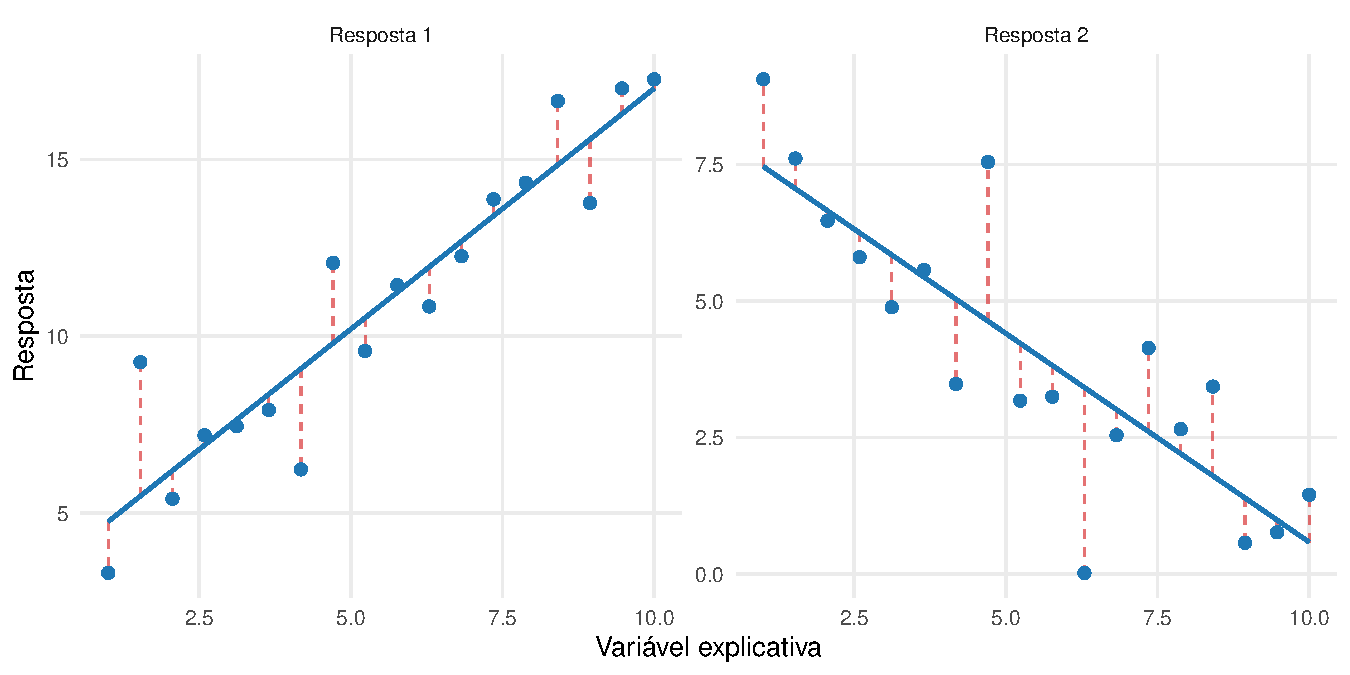
\includegraphics[keepaspectratio]{mod_2_modelo_files/figure-pdf/fig-ajustes-residuos-multivariados-1.pdf}}

}

\caption{\label{fig-ajustes-residuos-multivariados}Valores observados,
retas ajustadas e resíduos para duas respostas modeladas pela mesma
variável explicativa.}

\end{figure}%

Os segmentos verticais representam os resíduos de cada resposta. O mesmo
projetor \(\mathbf P_Z\) determina as posições ajustadas nas duas
colunas, enquanto a associação residual entre as respostas não é
representada diretamente nos painéis.

Essa associação será resumida pela SQPC residual.

\subsection{Conexão com o modelo contendo somente
intercepto}\label{conexuxe3o-com-o-modelo-contendo-somente-intercepto}

Quando

\[
\mathbf Z
=
\mathbf1_n,
\]

tem-se

\[
\mathbf P_Z
=
\frac{1}{n}
\mathbf1_n
\mathbf1_n^\top
\]

e

\begin{equation}\phantomsection\label{eq-projetores-modelo-somente-intercepto}{
\mathbf M_Z
=
\mathbf I_n
-
\frac{1}{n}
\mathbf1_n
\mathbf1_n^\top
=
\mathbf H_n.
}\end{equation}

Assim,

\[
\widehat{\mathbf Y}
=
\mathbf1_n
\bar{\mathbf y}^\top,
\]

enquanto

\[
\widehat{\mathbf U}
=
\mathbf H_n
\mathbf Y.
\]

A matriz residual coincide, nesse caso, com a matriz de respostas
centralizada. Portanto, a centralização utilizada nos Capítulos 8 e 10
aparece como um caso particular da projeção residual no modelo linear
multivariado.

A próxima seção utilizará

\[
\widehat{\mathbf U}
\]

para construir a SQPC residual, determinar seus graus de liberdade e
estimar a matriz de covariâncias \(\boldsymbol{\Sigma}\).

\section{SQPC residual e estimação da
covariância}\label{sqpc-residual-e-estimauxe7uxe3o-da-covariuxe2ncia}

A matriz de resíduos

\[
\widehat{\boldsymbol{\mathcal U}}
=
\mathbf M_Z
\boldsymbol{\mathcal Y}
\]

contém os desvios das respostas em relação aos valores ajustados pelo
modelo. Os produtos cruzados entre esses resíduos formam uma matriz que
descreve a dispersão conjunta que permanece após o ajuste e permite
estimar

\[
\boldsymbol{\Sigma},
\]

a matriz de covariâncias dos erros.

No modelo contendo somente intercepto, essa construção recupera a SQPC
amostral dos Capítulos 8 e 10. No modelo linear geral, o ajuste remove
um espaço de médias de dimensão

\[
r
=
\operatorname{posto}
\left(
\mathbf Z
\right),
\]

restando um espaço residual de dimensão \(n-r\).

\subsection{Construção da SQPC
residual}\label{construuxe7uxe3o-da-sqpc-residual}

\begin{definition}[SQPC
residual]\protect\hypertarget{def-sscp-residual-modelo-multivariado}{}\label{def-sscp-residual-modelo-multivariado}

A SQPC residual aleatória é

\begin{equation}\phantomsection\label{eq-sscp-residual-aleatoria}{
\boldsymbol{\mathsf E}_{\mathrm{res}}
=
\widehat{\boldsymbol{\mathcal U}}^\top
\widehat{\boldsymbol{\mathcal U}}.
}\end{equation}

Como

\[
\widehat{\boldsymbol{\mathcal U}}
=
\mathbf M_Z
\boldsymbol{\mathcal Y},
\]

e \(\mathbf M_Z\) é simétrica e idempotente,

\begin{equation}\phantomsection\label{eq-sscp-residual-aleatoria-projetor}{
\boldsymbol{\mathsf E}_{\mathrm{res}}
=
\boldsymbol{\mathcal Y}^\top
\mathbf M_Z
\boldsymbol{\mathcal Y}.
}\end{equation}

Após a observação,

\begin{equation}\phantomsection\label{eq-sscp-residual-observada}{
\mathbf E
=
\widehat{\mathbf U}^\top
\widehat{\mathbf U}
=
\mathbf Y^\top
\mathbf M_Z
\mathbf Y.
}\end{equation}

\end{definition}

O elemento \((j,k)\) de \(\mathbf E\) é

\begin{equation}\phantomsection\label{eq-elemento-sscp-residual}{
e_{jk}
=
\sum_{i=1}^{n}
\widehat u_{ij}
\widehat u_{ik}.
}\end{equation}

Para \(j=k\),

\[
e_{jj}
=
\sum_{i=1}^{n}
\widehat u_{ij}^{\,2}
\]

é a soma de quadrados residual da resposta \(j\). Para \(j\neq k\),
\(e_{jk}\) é o produto cruzado residual entre as respostas \(j\) e
\(k\).

Como

\[
\boldsymbol{\mathcal Y}
=
\mathbf Z\mathbf B
+
\boldsymbol{\mathcal E}
\]

e

\[
\mathbf M_Z\mathbf Z
=
\mathbf0,
\]

tem-se

\begin{equation}\phantomsection\label{eq-residuos-como-projecao-erros}{
\widehat{\boldsymbol{\mathcal U}}
=
\mathbf M_Z
\boldsymbol{\mathcal E},
}\end{equation}

e, consequentemente,

\begin{equation}\phantomsection\label{eq-sscp-residual-erros}{
\boldsymbol{\mathsf E}_{\mathrm{res}}
=
\boldsymbol{\mathcal E}^\top
\mathbf M_Z
\boldsymbol{\mathcal E}.
}\end{equation}

A SQPC residual depende do espaço de médias removido pelo ajuste por
meio de \(\mathbf M_Z\), mas não depende do valor específico de
\(\mathbf B\).

Como toda matriz de Gram, \(\mathbf E\) é simétrica e positiva
semidefinida. Para qualquer

\[
\mathbf a
\in
\mathbb R^p,
\]

\begin{equation}\phantomsection\label{eq-semidefinicao-sscp-residual}{
\begin{aligned}
\mathbf a^\top
\mathbf E
\mathbf a
&=
\left\|
\widehat{\mathbf U}
\mathbf a
\right\|^2
\\
&\geq
0.
\end{aligned}
}\end{equation}

A forma quadrática corresponde à soma de quadrados residual da
combinação linear das respostas

\[
\mathbf Y\mathbf a.
\]

De fato,

\[
\widehat{\mathbf u}_{\mathbf a}
=
\mathbf M_Z
\mathbf Y\mathbf a
=
\widehat{\mathbf U}\mathbf a,
\]

e

\begin{equation}\phantomsection\label{eq-soma-quadrados-residual-combinacao-respostas}{
\widehat{\mathbf u}_{\mathbf a}^\top
\widehat{\mathbf u}_{\mathbf a}
=
\mathbf a^\top
\mathbf E
\mathbf a.
}\end{equation}

Se as respostas forem transformadas por

\[
\mathbf Y^\ast
=
\mathbf Y\mathbf A,
\qquad
\mathbf A
\in
\mathbb R^{p\times s},
\]

então

\[
\widehat{\mathbf U}^{\ast}
=
\widehat{\mathbf U}\mathbf A
\]

e

\begin{equation}\phantomsection\label{eq-transformacao-sscp-residual-respostas}{
\mathbf E^\ast
=
\mathbf A^\top
\mathbf E
\mathbf A.
}\end{equation}

Essa transformação é coerente com a regra populacional

\[
\boldsymbol{\Sigma}^{\ast}
=
\mathbf A^\top
\boldsymbol{\Sigma}
\mathbf A
\]

e será utilizada posteriormente em hipóteses sobre combinações das
respostas.

\subsection{Esperança e graus de
liberdade}\label{esperanuxe7a-e-graus-de-liberdade}

A dimensão do espaço residual é determinada pelo posto da matriz de
delineamento.

Como

\[
\mathbf M_Z
=
\mathbf I_n-\mathbf P_Z,
\]

tem-se

\[
\operatorname{posto}
\left(
\mathbf M_Z
\right)
=
\operatorname{tr}
\left(
\mathbf M_Z
\right)
=
n-r.
\]

\begin{definition}[Graus de liberdade
residuais]\protect\hypertarget{def-graus-liberdade-residuais}{}\label{def-graus-liberdade-residuais}

Se

\[
r
=
\operatorname{posto}
\left(
\mathbf Z
\right),
\]

os graus de liberdade residuais são

\begin{equation}\phantomsection\label{eq-graus-liberdade-residuais}{
\nu_E
=
n-r.
}\end{equation}

\end{definition}

Quando \(\mathbf Z\) possui posto coluna completo,

\[
r=q,
\]

e, portanto,

\[
\nu_E
=
n-q.
\]

A expressão utiliza \(r\), e não simplesmente o número de colunas de
\(\mathbf Z\), porque somente as \(r\) direções linearmente
independentes do espaço do modelo consomem graus de liberdade. Colunas
redundantes não aumentam a dimensão do espaço de médias ajustado.

\begin{proposition}[Esperança da SQPC
residual]\protect\hypertarget{prp-esperanca-sscp-residual}{}\label{prp-esperanca-sscp-residual}

Sob a estrutura do modelo linear multivariado,

\[
E
\left(
\boldsymbol{\mathcal E}
\mid
\mathbf Z
\right)
=
\mathbf0,
\]

\[
\operatorname{Cov}
\left(
\boldsymbol{\varepsilon}_i
\mid
\mathbf Z
\right)
=
\boldsymbol{\Sigma},
\]

e

\[
\operatorname{Cov}
\left(
\boldsymbol{\varepsilon}_i,
\boldsymbol{\varepsilon}_\ell
\mid
\mathbf Z
\right)
=
\mathbf0,
\qquad
i\neq\ell,
\]

com

\[
r
=
\operatorname{posto}
\left(
\mathbf Z
\right),
\]

tem-se

\begin{equation}\phantomsection\label{eq-esperanca-sscp-residual}{
E
\left(
\boldsymbol{\mathsf E}_{\mathrm{res}}
\mid
\mathbf Z
\right)
=
(n-r)
\boldsymbol{\Sigma}.
}\end{equation}

\end{proposition}

\begin{proof}
Pela Equação~\ref{eq-sscp-residual-erros},

\[
\boldsymbol{\mathsf E}_{\mathrm{res}}
=
\boldsymbol{\mathcal E}^\top
\mathbf M_Z
\boldsymbol{\mathcal E}.
\]

Considere o elemento \((j,k)\):

\[
\left[
\boldsymbol{\mathsf E}_{\mathrm{res}}
\right]_{jk}
=
\boldsymbol{\varepsilon}_{\cdot j}^\top
\mathbf M_Z
\boldsymbol{\varepsilon}_{\cdot k}.
\]

Escrevendo

\[
\mathbf M_Z
=
(m_{i\ell}),
\]

obtém-se

\[
\left[
\boldsymbol{\mathsf E}_{\mathrm{res}}
\right]_{jk}
=
\sum_{i=1}^{n}
\sum_{\ell=1}^{n}
m_{i\ell}
\varepsilon_{ij}
\varepsilon_{\ell k}.
\]

Para \(i\neq\ell\),

\[
E
\left(
\varepsilon_{ij}
\varepsilon_{\ell k}
\mid
\mathbf Z
\right)
=
0,
\]

enquanto, para \(i=\ell\),

\[
E
\left(
\varepsilon_{ij}
\varepsilon_{ik}
\mid
\mathbf Z
\right)
=
\sigma_{jk}.
\]

Logo,

\[
\begin{aligned}
E
\left[
\left[
\boldsymbol{\mathsf E}_{\mathrm{res}}
\right]_{jk}
\mid
\mathbf Z
\right]
&=
\sum_{i=1}^{n}
m_{ii}
\sigma_{jk}
\\
&=
\operatorname{tr}
\left(
\mathbf M_Z
\right)
\sigma_{jk}
\\
&=
(n-r)
\sigma_{jk}.
\end{aligned}
\]

Como a igualdade vale para todos os elementos,

\[
E
\left(
\boldsymbol{\mathsf E}_{\mathrm{res}}
\mid
\mathbf Z
\right)
=
(n-r)
\boldsymbol{\Sigma}.
\]
\end{proof}

A expressão generaliza Proposição~\ref{prp-esperanca-sscp-amostral}, que
estabelece

\[
E
\left(
\boldsymbol{\mathsf T}
\right)
=
(n-1)
\boldsymbol{\Sigma}.
\]

No modelo contendo somente intercepto,

\[
r=1,
\]

de modo que

\[
n-r=n-1.
\]

No modelo linear geral, cada direção independente utilizada para
representar a estrutura de médias reduz em uma unidade a dimensão do
espaço residual.

\subsection{Estimação da covariância
residual}\label{estimauxe7uxe3o-da-covariuxe2ncia-residual}

\begin{definition}[Estimador residual da matriz de
covariâncias]\protect\hypertarget{def-estimador-nao-viesado-covariancia-residual}{}\label{def-estimador-nao-viesado-covariancia-residual}

Se

\[
r
=
\operatorname{posto}
\left(
\mathbf Z
\right)
\]

e

\[
n-r>0,
\]

define-se

\begin{equation}\phantomsection\label{eq-estimador-nao-viesado-covariancia-residual}{
\widehat{\boldsymbol{\Sigma}}
=
\frac{
\boldsymbol{\mathsf E}_{\mathrm{res}}
}{
n-r
}.
}\end{equation}

Após a observação,

\begin{equation}\phantomsection\label{eq-estimativa-nao-viesada-covariancia-residual}{
\widehat{\boldsymbol{\Sigma}}_{\mathrm{obs}}
=
\frac{
\mathbf E
}{
n-r
}.
}\end{equation}

\end{definition}

\begin{proposition}[Não viesamento do estimador
residual]\protect\hypertarget{prp-nao-viesamento-covariancia-residual}{}\label{prp-nao-viesamento-covariancia-residual}

Se

\[
r
=
\operatorname{posto}
\left(
\mathbf Z
\right),
\qquad
n-r>0,
\]

e

\[
E
\left(
\boldsymbol{\mathsf E}_{\mathrm{res}}
\mid
\mathbf Z
\right)
=
(n-r)
\boldsymbol{\Sigma},
\]

então

\begin{equation}\phantomsection\label{eq-nao-vies-covariancia-residual}{
E
\left(
\widehat{\boldsymbol{\Sigma}}
\mid
\mathbf Z
\right)
=
\boldsymbol{\Sigma}.
}\end{equation}

Portanto, \(\widehat{\boldsymbol{\Sigma}}\) é um estimador não viesado
da matriz de covariâncias dos erros.

\end{proposition}

\begin{proof}
Por Equação~\ref{eq-estimador-nao-viesado-covariancia-residual} e
Equação~\ref{eq-esperanca-sscp-residual},

\[
\begin{aligned}
E
\left(
\widehat{\boldsymbol{\Sigma}}
\mid
\mathbf Z
\right)
&=
\frac{1}{n-r}
E
\left(
\boldsymbol{\mathsf E}_{\mathrm{res}}
\mid
\mathbf Z
\right)
\\
&=
\frac{1}{n-r}
(n-r)
\boldsymbol{\Sigma}
\\
&=
\boldsymbol{\Sigma}.
\end{aligned}
\]
\end{proof}

Componente a componente,

\begin{equation}\phantomsection\label{eq-elemento-covariancia-residual-estimada}{
\widehat{\sigma}_{jk,\mathrm{obs}}
=
\frac{e_{jk}}{n-r}.
}\end{equation}

Assim,

\[
\widehat{\sigma}_{jj,\mathrm{obs}}
=
\frac{1}{n-r}
\sum_{i=1}^{n}
\widehat u_{ij}^{\,2}
\]

estima a variância residual da resposta \(j\), enquanto, para
\(j\neq k\),

\[
\widehat{\sigma}_{jk,\mathrm{obs}}
=
\frac{1}{n-r}
\sum_{i=1}^{n}
\widehat u_{ij}
\widehat u_{ik}
\]

estima a covariância residual entre as respostas \(j\) e \(k\).

A matriz de correlações residuais pode ser obtida pela mesma
padronização utilizada nos Capítulos 8 e 10, desde que as variâncias
residuais estimadas sejam positivas. Não é necessário introduzir uma
nova construção: aplica-se

\[
\mathbf D^{-1/2}
\widehat{\boldsymbol{\Sigma}}_{\mathrm{obs}}
\mathbf D^{-1/2}
\]

com a matriz diagonal correspondente às variâncias residuais estimadas.

\begin{tcolorbox}[enhanced jigsaw, colback=white, breakable, bottomrule=.15mm, left=2mm, arc=.35mm, rightrule=.15mm, colframe=quarto-callout-note-color-frame, toprule=.15mm, leftrule=.75mm, opacityback=0]

\vspace{-3mm}\textbf{Covariância total e covariância residual}\vspace{3mm}

A matriz de covariâncias calculada diretamente das respostas descreve a
variabilidade conjunta observada antes do ajuste.

A matriz

\[
\widehat{\boldsymbol{\Sigma}}_{\mathrm{obs}}
\]

descreve a variabilidade que permanece depois de removida a estrutura de
médias pertencente a

\[
\mathcal C
\left(
\mathbf Z
\right).
\]

Por isso, em geral, as duas matrizes não coincidem.

\end{tcolorbox}

\subsection{Estimador de máxima
verossimilhança}\label{estimador-de-muxe1xima-verossimilhanuxe7a-1}

Sob o modelo normal matricial, depois da maximização em relação à
estrutura de médias, a parte da log-verossimilhança que depende de
\(\boldsymbol{\Sigma}\) é, a menos de constantes,

\begin{equation}\phantomsection\label{eq-logverossimilhanca-concentrada-covariancia-residual}{
\ell_c
\left(
\boldsymbol{\Sigma}
\right)
=
-\frac{n}{2}
\log
\det
\left(
\boldsymbol{\Sigma}
\right)
-
\frac{1}{2}
\operatorname{tr}
\left(
\boldsymbol{\Sigma}^{-1}
\mathbf E
\right).
}\end{equation}

Quando

\[
\mathbf E
\succ
\mathbf0,
\]

o máximo no espaço

\[
\boldsymbol{\Sigma}
\succ
\mathbf0
\]

é alcançado em

\begin{equation}\phantomsection\label{eq-estimativa-mv-covariancia-residual}{
\widehat{\boldsymbol{\Sigma}}_{\mathrm{MV,obs}}
=
\frac{\mathbf E}{n}.
}\end{equation}

Como

\[
E
\left(
\boldsymbol{\mathsf E}_{\mathrm{res}}
\mid
\mathbf Z
\right)
=
(n-r)
\boldsymbol{\Sigma},
\]

a estatística com divisor \(n\) satisfaz

\[
E
\left(
\frac{
\boldsymbol{\mathsf E}_{\mathrm{res}}
}{n}
\mid
\mathbf Z
\right)
=
\frac{n-r}{n}
\boldsymbol{\Sigma}.
\]

Portanto, seu viés é

\[
-\frac{r}{n}
\boldsymbol{\Sigma}.
\]

Assim, o divisor \(n-r\) produz o estimador não viesado, enquanto o
divisor \(n\) é utilizado pela máxima verossimilhança sob normalidade e
existência do máximo. Essa relação generaliza
Equação~\ref{eq-relacao-mv-covariancia-nao-viesada}, na qual os
divisores correspondentes são \(n-1\) e \(n\).

\begin{tcolorbox}[enhanced jigsaw, colback=white, breakable, bottomrule=.15mm, left=2mm, arc=.35mm, rightrule=.15mm, colframe=quarto-callout-caution-color-frame, toprule=.15mm, leftrule=.75mm, opacityback=0]

\vspace{-3mm}\textbf{Existência do estimador de máxima verossimilhança}\vspace{3mm}

A expressão

\[
\frac{\mathbf E}{n}
\]

é a estimativa de máxima verossimilhança de \(\boldsymbol{\Sigma}\) no
modelo normal não singular somente quando

\[
\mathbf E
\succ
\mathbf0.
\]

Se \(\mathbf E\) é singular, a verossimilhança não possui máximo no
interior do espaço

\[
\boldsymbol{\Sigma}
\succ
\mathbf0.
\]

A matriz \(\mathbf E/n\) continua sendo calculável, mas perde essa
interpretação de máxima verossimilhança no modelo positivo definido.

\end{tcolorbox}

\subsection{Posto e singularidade}\label{posto-e-singularidade}

A SQPC residual possui a forma de Gram

\[
\mathbf E
=
\widehat{\mathbf U}^\top
\widehat{\mathbf U}.
\]

Portanto,

\[
\operatorname{posto}
\left(
\mathbf E
\right)
=
\operatorname{posto}
\left(
\widehat{\mathbf U}
\right).
\]

Como

\[
\widehat{\mathbf U}
=
\mathbf M_Z\mathbf Y
\]

e

\[
\operatorname{posto}
\left(
\mathbf M_Z
\right)
=
n-r,
\]

obtém-se:

\begin{proposition}[Posto da SQPC
residual]\protect\hypertarget{prp-posto-sscp-residual}{}\label{prp-posto-sscp-residual}

Se

\[
r
=
\operatorname{posto}
\left(
\mathbf Z
\right),
\]

a SQPC residual observada

\[
\mathbf E
=
\mathbf Y^\top
\mathbf M_Z
\mathbf Y
\]

satisfaz

\begin{equation}\phantomsection\label{eq-posto-sscp-residual}{
\operatorname{posto}
\left(
\mathbf E
\right)
\leq
\min
\left(
p,n-r
\right).
}\end{equation}

\end{proposition}

Consequentemente, se

\[
p>n-r,
\]

então \(\mathbf E\) é necessariamente singular.

Uma condição necessária para

\[
\mathbf E
\succ
\mathbf0
\]

é

\begin{equation}\phantomsection\label{eq-condicao-necessaria-covariancia-residual-positiva}{
n-r
\geq
p.
}\end{equation}

Para uma amostra arbitrária, essa desigualdade não é suficiente: também
é necessário

\[
\operatorname{posto}
\left(
\widehat{\mathbf U}
\right)
=
p.
\]

Portanto, uma condição necessária para que a SQPC residual seja positiva
definida é haver pelo menos \(p\) dimensões residuais,

\[
n-r
\geq
p.
\]

A desigualdade, isoladamente, não garante posto completo em uma amostra
arbitrária; também é necessário que os resíduos observados gerem \(p\)
direções linearmente independentes.

O limite de posto é a extensão de Equação~\ref{eq-posto-sscp-amostral},
que no caso de uma única média fornece

\[
\operatorname{posto}
\left(
\mathbf S
\right)
\leq
\min
\left(
p,n-1
\right).
\]

Questões de condicionamento, pseudoinversa e regularização continuam
pertinentes às matrizes residuais, mas não serão novamente desenvolvidas
aqui. O condicionamento foi discutido em
Equação~\ref{eq-numero-condicao-covariancia}, a pseudoinversa em
Equação~\ref{eq-pseudoinversa-covariancia-amostral} e a regularização
por contração em Definição~\ref{def-estimador-contracao-covariancia}.

\subsection{Modelo contendo somente
intercepto}\label{modelo-contendo-somente-intercepto-1}

Considere

\[
\mathbf Z
=
\mathbf1_n.
\]

Nesse caso,

\[
r=1,
\]

\[
\mathbf P_Z
=
\frac{1}{n}
\mathbf1_n
\mathbf1_n^\top
\]

e

\[
\mathbf M_Z
=
\mathbf H_n.
\]

Logo,

\[
\widehat{\mathbf U}
=
\mathbf H_n
\mathbf Y,
\]

e a SQPC residual observada é

\begin{equation}\phantomsection\label{eq-sscp-residual-modelo-intercepto}{
\begin{aligned}
\mathbf E
&=
\mathbf Y^\top
\mathbf H_n
\mathbf Y
\\
&=
\sum_{i=1}^{n}
\left(
\mathbf y_i-\bar{\mathbf y}
\right)
\left(
\mathbf y_i-\bar{\mathbf y}
\right)^\top.
\end{aligned}
}\end{equation}

Essa matriz é exatamente a SQPC total observada

\[
\mathbf T
\]

definida em Definição~\ref{def-matriz-sscp-total} e correspondente à
realização da estatística aleatória definida em
Definição~\ref{def-sscp-amostral-aleatoria}.

Como

\[
n-r
=
n-1,
\]

obtém-se

\begin{equation}\phantomsection\label{eq-covariancia-residual-modelo-intercepto}{
\widehat{\boldsymbol{\Sigma}}_{\mathrm{obs}}
=
\frac{\mathbf E}{n-1}
=
\mathbf S,
}\end{equation}

recuperando Definição~\ref{def-matriz-covariancias-amostral-aleatoria}.

Sob normalidade e quando a SQPC possui posto completo,

\[
\widehat{\boldsymbol{\Sigma}}_{\mathrm{MV,obs}}
=
\frac{\mathbf E}{n},
\]

em concordância com Equação~\ref{eq-mv-covariancia-normal}.

Portanto, no modelo contendo somente intercepto,

\[
\mathbf E
=
\mathbf T
\]

e

\[
\frac{\mathbf E}{n-1}
=
\mathbf S.
\]

Assim, a SQPC residual e o estimador não viesado da covariância residual
recuperam exatamente os objetos estudados nos Capítulos 8 e 10. O modelo
linear multivariado substitui a remoção de uma única média pela remoção
de toda a estrutura de médias representada por

\[
\mathcal C
\left(
\mathbf Z
\right).
\]

A próxima seção separa a SQPC total em uma parcela associada ao modelo e
uma parcela residual.

\section{Decomposição da variação
multivariada}\label{decomposiuxe7uxe3o-da-variauxe7uxe3o-multivariada}

Quando o espaço coluna de \(\mathbf Z\) contém o vetor \(\mathbf1_n\), a
dispersão das respostas em torno do vetor de médias amostrais pode ser
decomposta em uma parcela associada ao modelo e uma parcela residual.
Essa condição é satisfeita, por exemplo, quando o modelo possui um
intercepto explícito e também em parametrizações nas quais a média geral
pertence ao espaço do modelo sem corresponder a uma coluna específica de
\(\mathbf Z\).

No caso univariado, essa separação produz as somas de quadrados
utilizadas na análise de variância. No modelo multivariado, cada parcela
é representada por uma matriz SQPC, preservando também os produtos
cruzados entre as respostas.

A principal decomposição é

\[
\mathbf T
=
\mathbf T_{\mathrm{mod}}
+
\mathbf E,
\]

em que \(\mathbf T\) representa a dispersão total em torno da média
geral, \(\mathbf T_{\mathrm{mod}}\) representa a dispersão dos valores
ajustados em torno da média geral e \(\mathbf E\) representa a dispersão
residual em torno dos valores ajustados.

\subsection{SQPC total}\label{sqpc-total}

A SQPC total observada foi definida em
Definição~\ref{def-matriz-sscp-total}. Aplicada à matriz de respostas,

\begin{equation}\phantomsection\label{eq-sscp-total-modelo-multivariado}{
\mathbf T
=
\mathbf Y^\top
\mathbf H_n
\mathbf Y,
}\end{equation}

em que \(\mathbf H_n\) é a matriz de centralização utilizada em
Equação~\ref{eq-centralizacao-por-hn}:

\[
\mathbf H_n
=
\mathbf I_n
-
\frac{1}{n}
\mathbf1_n\mathbf1_n^\top.
\]

Equivalentemente,

\begin{equation}\phantomsection\label{eq-sscp-total-somatorio}{
\mathbf T
=
\sum_{i=1}^{n}
\left(
\mathbf y_i-\bar{\mathbf y}
\right)
\left(
\mathbf y_i-\bar{\mathbf y}
\right)^\top,
}\end{equation}

com

\[
\bar{\mathbf y}
=
\frac{1}{n}
\mathbf Y^\top
\mathbf1_n.
\]

A matriz \(\mathbf T\) descreve a dispersão conjunta das respostas antes
da remoção da estrutura explicada pelo delineamento.

\subsection{SQPC associada ao modelo}\label{sqpc-associada-ao-modelo}

Suponha que a direção constante pertença ao espaço do modelo, isto é,

\begin{equation}\phantomsection\label{eq-condicao-intercepto-espaco-modelo}{
\mathbf1_n
\in
\mathcal C
\left(
\mathbf Z
\right).
}\end{equation}

Essa condição é satisfeita quando o modelo possui um intercepto
explícito e também em parametrizações nas quais a média geral pertence
ao espaço do modelo sem corresponder a uma coluna específica de
\(\mathbf Z\).

Defina o projetor sobre o espaço das constantes por

\begin{equation}\phantomsection\label{eq-projetor-intercepto}{
\mathbf P_1
=
\frac{1}{n}
\mathbf1_n
\mathbf1_n^\top.
}\end{equation}

Como

\[
\mathcal C
\left(
\mathbf1_n
\right)
\subseteq
\mathcal C
\left(
\mathbf Z
\right),
\]

tem-se

\begin{equation}\phantomsection\label{eq-relacao-projetores-intercepto-modelo}{
\mathbf P_Z\mathbf P_1
=
\mathbf P_1\mathbf P_Z
=
\mathbf P_1.
}\end{equation}

Consequentemente,

\[
\mathbf P_Z-\mathbf P_1
\]

é o projetor ortogonal sobre a parte de \(\mathcal C(\mathbf Z)\)
ortogonal à direção constante. Essa parte representa as variações
ajustadas pelo modelo em torno da média geral.

Seu posto é

\begin{equation}\phantomsection\label{eq-posto-projetor-modelo-corrigido}{
\operatorname{posto}
\left(
\mathbf P_Z-\mathbf P_1
\right)
=
r-1,
}\end{equation}

em que

\[
r
=
\operatorname{posto}
\left(
\mathbf Z
\right).
\]

\begin{definition}[SQPC associada ao modelo, corrigida pela média
geral]\protect\hypertarget{def-sscp-modelo-corrigida}{}\label{def-sscp-modelo-corrigida}

Quando

\[
\mathbf1_n
\in
\mathcal C
\left(
\mathbf Z
\right),
\]

define-se

\begin{equation}\phantomsection\label{eq-sscp-modelo-corrigida}{
\mathbf T_{\mathrm{mod}}
=
\mathbf Y^\top
\left(
\mathbf P_Z-\mathbf P_1
\right)
\mathbf Y.
}\end{equation} em que \(\mathbf P_Z\) é o projetor sobre
\(\mathcal C(\mathbf Z)\) e

\[
\mathbf P_1
=
\frac{1}{n}
\mathbf1_n
\mathbf1_n^\top
\]

é o projetor sobre a direção constante.

\end{definition}

Se

\[
\mathcal C
\left(
\mathbf Z
\right)
=
\mathcal C
\left(
\mathbf1_n
\right),
\]

então

\[
\mathbf P_Z
=
\mathbf P_1
\]

e, consequentemente,

\[
\mathbf T_{\mathrm{mod}}
=
\mathbf0.
\]

Assim, \(\mathbf T_{\mathrm{mod}}\) quantifica somente a variação
ajustada que excede a representação da média geral.

A matriz

\[
\mathbf T_{\mathrm{mod}}
\]

mede a dispersão dos valores ajustados pelo modelo em torno da média
geral. No modelo de grupos, essa matriz coincide com a dispersão entre
grupos. Em modelos com covariáveis, ela representa conjuntamente a
variação dos valores ajustados em torno da média geral.

Se

\[
\widehat{\mathbf Y}
=
\mathbf P_Z\mathbf Y,
\]

então os valores ajustados centralizados são

\[
\widehat{\mathbf Y}_c
=
\widehat{\mathbf Y}
-
\mathbf1_n
\bar{\mathbf y}^\top
=
\left(
\mathbf P_Z-\mathbf P_1
\right)
\mathbf Y.
\]

Logo,

\begin{equation}\phantomsection\label{eq-sscp-modelo-ajustes-centralizados}{
\mathbf T_{\mathrm{mod}}
=
\widehat{\mathbf Y}_c^\top
\widehat{\mathbf Y}_c.
}\end{equation}

Para qualquer combinação linear das respostas,

\begin{equation}\phantomsection\label{eq-sscp-modelo-combinacao-respostas}{
\mathbf a^\top
\mathbf T_{\mathrm{mod}}
\mathbf a
=
\left\|
\left(
\mathbf P_Z-\mathbf P_1
\right)
\mathbf Y\mathbf a
\right\|^2.
}\end{equation}

Portanto, \(\mathbf T_{\mathrm{mod}}\) reúne, para todas as combinações
lineares das respostas, as somas de quadrados dos valores ajustados em
torno da respectiva média geral.

\subsection{Decomposição entre modelo e
resíduo}\label{decomposiuxe7uxe3o-entre-modelo-e-resuxedduo}

Sob a condição

\[
\mathbf1_n
\in
\mathcal C
\left(
\mathbf Z
\right),
\]

considere

\[
\mathbf H_n
=
\mathbf I_n-\mathbf P_1
\]

e

\[
\mathbf I_n
=
\mathbf P_Z+\mathbf M_Z.
\]

segue que

\begin{equation}\phantomsection\label{eq-decomposicao-projetor-centralizacao}{
\mathbf H_n
=
\left(
\mathbf P_Z-\mathbf P_1
\right)
+
\mathbf M_Z.
}\end{equation}

Além disso,

\[
\left(
\mathbf P_Z-\mathbf P_1
\right)
\mathbf M_Z
=
\mathbf0.
\]

Assim, as duas parcelas correspondem a subespaços ortogonais.

\begin{proposition}[Decomposição da SQPC
total]\protect\hypertarget{prp-decomposicao-sscp-modelo-multivariado}{}\label{prp-decomposicao-sscp-modelo-multivariado}

Se

\[
\mathbf1_n
\in
\mathcal C
\left(
\mathbf Z
\right),
\]

então

\begin{equation}\phantomsection\label{eq-decomposicao-sscp-total-modelo-residuo}{
\mathbf T
=
\mathbf T_{\mathrm{mod}}
+
\mathbf E,
}\end{equation}

em que

\[
\mathbf T
=
\mathbf Y^\top
\mathbf H_n
\mathbf Y,
\]

\[
\mathbf T_{\mathrm{mod}}
=
\mathbf Y^\top
\left(
\mathbf P_Z-\mathbf P_1
\right)
\mathbf Y
\]

e

\[
\mathbf E
=
\mathbf Y^\top
\mathbf M_Z
\mathbf Y.
\]

\end{proposition}

\begin{proof}
Substituindo Equação~\ref{eq-decomposicao-projetor-centralizacao} na
definição de \(\mathbf T\),

\[
\begin{aligned}
\mathbf T
&=
\mathbf Y^\top
\mathbf H_n
\mathbf Y
\\
&=
\mathbf Y^\top
\left[
\left(
\mathbf P_Z-\mathbf P_1
\right)
+
\mathbf M_Z
\right]
\mathbf Y
\\
&=
\mathbf T_{\mathrm{mod}}
+
\mathbf E.
\end{aligned}
\]
\end{proof}

A decomposição pode ser escrita também como

\begin{equation}\phantomsection\label{eq-decomposicao-sscp-somatorios}{
\begin{aligned}
&
\sum_{i=1}^{n}
\left(
\mathbf y_i-\bar{\mathbf y}
\right)
\left(
\mathbf y_i-\bar{\mathbf y}
\right)^\top
\\
&=
\sum_{i=1}^{n}
\left(
\widehat{\mathbf y}_i-\bar{\mathbf y}
\right)
\left(
\widehat{\mathbf y}_i-\bar{\mathbf y}
\right)^\top
\\
&\quad+
\sum_{i=1}^{n}
\left(
\mathbf y_i-\widehat{\mathbf y}_i
\right)
\left(
\mathbf y_i-\widehat{\mathbf y}_i
\right)^\top.
\end{aligned}
}\end{equation}

A primeira parcela à direita é \(\mathbf T_{\mathrm{mod}}\) e a segunda
é \(\mathbf E\).

As dimensões dos subespaços correspondentes fornecem

\begin{equation}\phantomsection\label{eq-decomposicao-graus-liberdade-modelo}{
n-1
=
(r-1)
+
(n-r).
}\end{equation}

A Tabela Tabela~\ref{tbl-decomposicao-graus-liberdade-modelo} resume as
dimensões dos três subespaços envolvidos.

\begin{longtable}[]{@{}
  >{\raggedright\arraybackslash}p{(\linewidth - 4\tabcolsep) * \real{0.3000}}
  >{\raggedright\arraybackslash}p{(\linewidth - 4\tabcolsep) * \real{0.3000}}
  >{\raggedleft\arraybackslash}p{(\linewidth - 4\tabcolsep) * \real{0.4000}}@{}}
\caption{Decomposição das dimensões associadas à SQPC total quando a
direção constante pertence ao espaço do
modelo.}\label{tbl-decomposicao-graus-liberdade-modelo}\tabularnewline
\toprule\noalign{}
\begin{minipage}[b]{\linewidth}\raggedright
Fonte
\end{minipage} & \begin{minipage}[b]{\linewidth}\raggedright
Projetor
\end{minipage} & \begin{minipage}[b]{\linewidth}\raggedleft
Graus de liberdade
\end{minipage} \\
\midrule\noalign{}
\endfirsthead
\toprule\noalign{}
\begin{minipage}[b]{\linewidth}\raggedright
Fonte
\end{minipage} & \begin{minipage}[b]{\linewidth}\raggedright
Projetor
\end{minipage} & \begin{minipage}[b]{\linewidth}\raggedleft
Graus de liberdade
\end{minipage} \\
\midrule\noalign{}
\endhead
\bottomrule\noalign{}
\endlastfoot
Total corrigido pela média geral & \(\mathbf H_n\) & \(n-1\) \\
Modelo corrigido pela média geral & \(\mathbf P_Z-\mathbf P_1\) &
\(r-1\) \\
Residual & \(\mathbf M_Z\) & \(n-r\) \\
\end{longtable}

Os graus de liberdade correspondem aos postos dos projetores no espaço
das unidades. Eles não devem ser confundidos com os postos das matrizes
de SQPC, que também dependem de \(p\).

Em particular,

\[
\operatorname{posto}
\left(
\mathbf T
\right)
\leq
\min
\left(
p,n-1
\right),
\]

\[
\operatorname{posto}
\left(
\mathbf T_{\mathrm{mod}}
\right)
\leq
\min
\left(
p,r-1
\right),
\]

e

\begin{equation}\phantomsection\label{eq-postos-sscp-decomposicao-modelo}{
\operatorname{posto}
\left(
\mathbf E
\right)
\leq
\min
\left(
p,n-r
\right).
}\end{equation}

\subsection{Combinações lineares das
respostas}\label{combinauxe7uxf5es-lineares-das-respostas}

A decomposição matricial contém, simultaneamente, as decomposições
correspondentes a todas as combinações lineares das respostas.

Para

\[
\mathbf a
\in
\mathbb R^p,
\]

tem-se

\begin{equation}\phantomsection\label{eq-decomposicao-somas-quadrados-combinacao}{
\mathbf a^\top
\mathbf T
\mathbf a
=
\mathbf a^\top
\mathbf T_{\mathrm{mod}}
\mathbf a
+
\mathbf a^\top
\mathbf E
\mathbf a.
}\end{equation}

Cada termo possui interpretação univariada:

\[
\mathbf a^\top
\mathbf T
\mathbf a
\]

é a soma de quadrados total de \(\mathbf Y\mathbf a\),

\[
\mathbf a^\top
\mathbf T_{\mathrm{mod}}
\mathbf a
\]

é a soma de quadrados associada ao modelo, e

\[
\mathbf a^\top
\mathbf E
\mathbf a
\]

é a soma de quadrados residual.

Essa relação é suficiente, neste capítulo, para mostrar como a
decomposição matricial preserva simultaneamente as decomposições das
respostas originais e de suas combinações lineares. A utilização
conjunta dessas matrizes em procedimentos inferenciais será desenvolvida
no Capítulo 12 e, posteriormente, na formulação das técnicas
multivariadas.

\subsection{Modelos sem intercepto}\label{modelos-sem-intercepto}

Se

\[
\mathbf1_n
\notin
\mathcal C
\left(
\mathbf Z
\right),
\]

a decomposição corrigida

\[
\mathbf T
=
\mathbf T_{\mathrm{mod}}
+
\mathbf E
\]

não se aplica na forma anterior, porque \(\mathbf P_Z-\mathbf P_1\) não
é, em geral, um projetor.

Permanece válida a decomposição em relação à origem,

\begin{equation}\phantomsection\label{eq-decomposicao-nao-corrigida-modelo}{
\mathbf Y^\top
\mathbf Y
=
\mathbf Y^\top
\mathbf P_Z
\mathbf Y
+
\mathbf Y^\top
\mathbf M_Z
\mathbf Y.
}\end{equation}

Essa identidade não deve ser interpretada como uma decomposição da
dispersão em torno da média amostral. No restante deste capítulo, a
decomposição total--modelo--resíduo será utilizada principalmente quando
a direção constante pertence ao espaço coluna de \(\mathbf Z\).

\subsection{Modelo de grupos como caso
particular}\label{modelo-de-grupos-como-caso-particular}

Considere \(K\) grupos não vazios. Uma parametrização particularmente
simples utiliza uma coluna indicadora para cada grupo. Para três grupos,
por exemplo, a matriz de delineamento possui a forma

\[
\mathbf Z
=
\begin{bmatrix}
1 & 0 & 0\\
\vdots & \vdots & \vdots\\
1 & 0 & 0\\
0 & 1 & 0\\
\vdots & \vdots & \vdots\\
0 & 1 & 0\\
0 & 0 & 1\\
\vdots & \vdots & \vdots\\
0 & 0 & 1
\end{bmatrix},
\]

em que cada linha identifica o grupo da respectiva unidade.

Na parametrização por médias de grupos,

\[
\mathbf B
=
\begin{bmatrix}
\boldsymbol{\mu}_1^\top\\
\vdots\\
\boldsymbol{\mu}_K^\top
\end{bmatrix},
\]

em que \(\mathcal I_k\) representa o conjunto dos índices das unidades
pertencentes ao grupo \(k\). Assim,

\[
E
\left(
\boldsymbol{\mathsf Y}_i
\mid
i\in\mathcal I_k
\right)
=
\boldsymbol{\mu}_k.
\]

O estimador de mínimos quadrados é

\begin{equation}\phantomsection\label{eq-estimativa-medias-grupos}{
\widehat{\mathbf B}_{\mathrm{obs}}
=
\begin{bmatrix}
\bar{\mathbf y}_1^\top\\
\vdots\\
\bar{\mathbf y}_K^\top
\end{bmatrix}.
}\end{equation}

Portanto, o vetor ajustado para cada unidade é a média amostral do grupo
ao qual ela pertence.

A SQPC residual é

\begin{equation}\phantomsection\label{eq-sscp-intragrupos-modelo}{
\mathbf E
=
\sum_{k=1}^{K}
\sum_{i\in\mathcal I_k}
\left(
\mathbf y_i-\bar{\mathbf y}_k
\right)
\left(
\mathbf y_i-\bar{\mathbf y}_k
\right)^\top.
}\end{equation}

Pela definição de dispersão intragrupos em
Definição~\ref{def-sscp-intragrupos},

\begin{equation}\phantomsection\label{eq-correspondencia-sscp-residual-intragrupos}{
\mathbf E
=
\mathbf T_{\mathrm{intra}}.
}\end{equation}

Assim, a SQPC residual do modelo de grupos mede exatamente a dispersão
das observações em torno das médias de seus respectivos grupos.

A parcela associada ao modelo é

\begin{equation}\phantomsection\label{eq-sscp-entre-grupos-modelo}{
\mathbf T_{\mathrm{mod}}
=
\sum_{k=1}^{K}
n_k
\left(
\bar{\mathbf y}_k-\bar{\mathbf y}
\right)
\left(
\bar{\mathbf y}_k-\bar{\mathbf y}
\right)^\top.
}\end{equation}

Por Definição~\ref{def-sscp-entre-grupos},

\begin{equation}\phantomsection\label{eq-correspondencia-sscp-modelo-entregrupos}{
\mathbf T_{\mathrm{mod}}
=
\mathbf T_{\mathrm{entre}}.
}\end{equation}

Portanto,

\begin{equation}\phantomsection\label{eq-decomposicao-total-entre-dentro-grupos}{
\mathbf T
=
\mathbf T_{\mathrm{entre}}
+
\mathbf T_{\mathrm{intra}},
}\end{equation}

recuperando Proposição~\ref{prp-decomposicao-dispersao-grupos} como um
caso particular do modelo linear multivariado.

Os graus de liberdade também se decompõem como

\begin{equation}\phantomsection\label{eq-graus-liberdade-modelo-grupos}{
n-1
=
(K-1)
+
(n-K).
}\end{equation}

A Figura~\ref{fig-decomposicao-grupos-modelo} representa geometricamente
as duas parcelas dessa decomposição. Os segmentos que ligam cada
observação à média de seu grupo representam desvios intragrupos,
enquanto os segmentos tracejados que ligam as médias dos grupos à média
geral representam os deslocamentos responsáveis pela dispersão entre
grupos.

\begin{figure}

\centering{

\pandocbounded{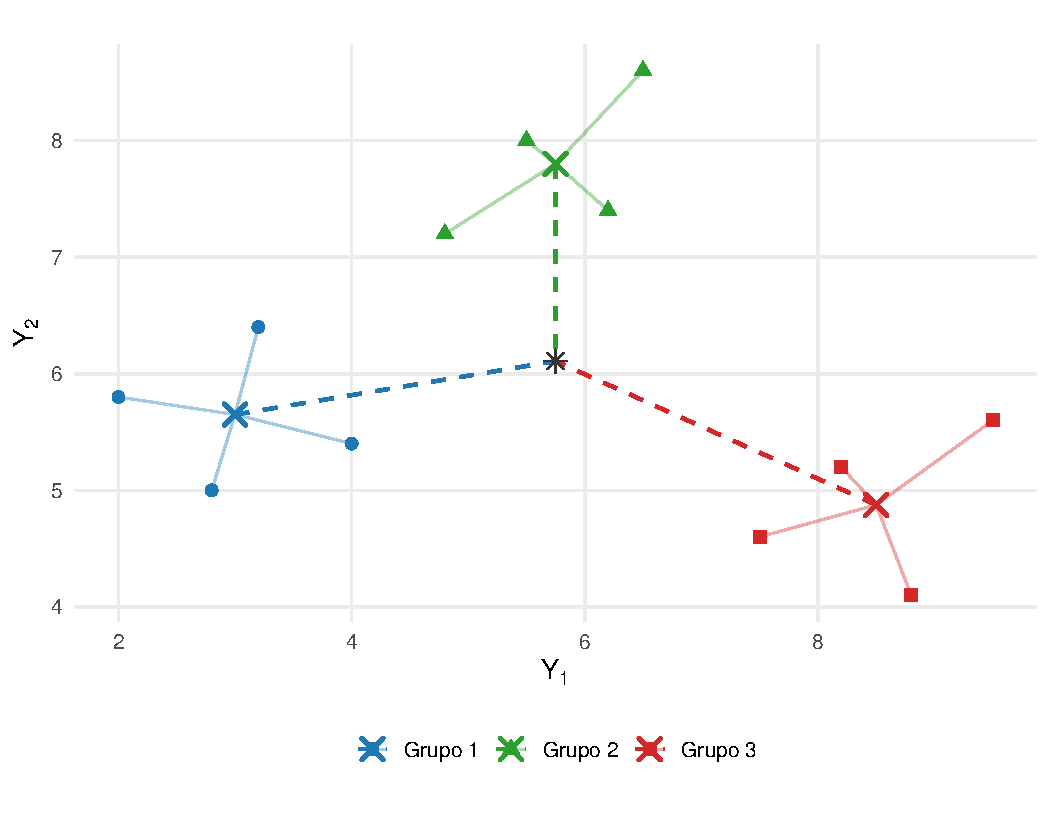
\includegraphics[keepaspectratio]{mod_2_modelo_files/figure-pdf/fig-decomposicao-grupos-modelo-1.pdf}}

}

\caption{\label{fig-decomposicao-grupos-modelo}Dispersão intragrupos e
deslocamento das médias dos grupos em relação à média geral.}

\end{figure}%

As cruzes representam as médias dos grupos e o asterisco representa a
média geral. Os segmentos internos aos grupos visualizam os termos
associados a \(\mathbf T_{\mathrm{intra}}\), enquanto os deslocamentos
das médias dos grupos em relação à média geral visualizam a estrutura
associada a \(\mathbf T_{\mathrm{entre}}\).

A decomposição depende do espaço de médias representado por
\(\mathbf Z\), e não de uma parametrização específica desse espaço. Essa
distinção motiva a discussão de posto, parametrização e estimabilidade
da próxima seção.

\section{Posto, parametrização e
estimabilidade}\label{posto-parametrizauxe7uxe3o-e-estimabilidade}

A expressão

\[
\widehat{\mathbf B}
=
\left(
\mathbf Z^\top
\mathbf Z
\right)^{-1}
\mathbf Z^\top
\boldsymbol{\mathcal Y}
\]

exige

\[
\operatorname{posto}
\left(
\mathbf Z
\right)
=
q.
\]

Nesse caso, as colunas de \(\mathbf Z\) são linearmente independentes e
os coeficientes de \(\mathbf B\) são determinados pela parametrização
adotada.

Alguns modelos, especialmente aqueles que representam grupos ou fatores,
podem ser escritos com colunas redundantes em \(\mathbf Z\). Diferentes
valores dos coeficientes podem então representar exatamente a mesma
estrutura de médias

\[
\mathbf Z\mathbf B.
\]

Por isso, é necessário distinguir a unicidade dos coeficientes da
unicidade dos valores ajustados e das combinações de parâmetros que se
deseja interpretar.

\subsection{Delineamento com posto
deficiente}\label{delineamento-com-posto-deficiente}

Considere

\[
\mathbf Z
\in
\mathbb R^{n\times q}
\]

com

\begin{equation}\phantomsection\label{eq-posto-deficiente-delineamento}{
r
=
\operatorname{posto}
\left(
\mathbf Z
\right)
<
q.
}\end{equation}

Nesse caso, as colunas de \(\mathbf Z\) são linearmente dependentes.
Portanto, existe pelo menos um vetor não nulo

\[
\mathbf d
\in
\mathbb R^q
\]

tal que

\[
\mathbf Z\mathbf d
=
\mathbf0.
\]

Consequentemente, alterações dos coeficientes em direções pertencentes
ao núcleo de \(\mathbf Z\) não modificam a estrutura de médias.

\begin{definition}[Matrizes de parâmetros
equivalentes]\protect\hypertarget{def-equivalencia-matrizes-parametros}{}\label{def-equivalencia-matrizes-parametros}

Duas matrizes

\[
\mathbf B_1,
\mathbf B_2
\in
\mathbb R^{q\times p}
\]

são equivalentes em relação a \(\mathbf Z\) quando

\begin{equation}\phantomsection\label{eq-definicao-equivalencia-parametros}{
\mathbf Z\mathbf B_1
=
\mathbf Z\mathbf B_2.
}\end{equation}

\end{definition}

Assim, quando \(r<q\), os coeficientes individuais de \(\mathbf B\)
podem não ser únicos, embora a matriz de médias

\[
\mathbf Z\mathbf B
\]

continue unicamente determinada pelo modelo.

\subsection{Pseudoinversa e unicidade do
ajuste}\label{pseudoinversa-e-unicidade-do-ajuste}

A pseudoinversa de Moore--Penrose e sua relação com mínimos quadrados
foram desenvolvidas em Definição~\ref{def-pseudoinversa-svd} e
Proposição~\ref{prp-minimos-quadrados-pseudoinversa}.

Quando

\[
r<q,
\]

a matriz

\[
\mathbf Z^\top\mathbf Z
\]

é singular, mas o problema de mínimos quadrados continua tendo solução.
Uma delas é

\begin{equation}\phantomsection\label{eq-estimador-pseudoinversa-parametros}{
\widehat{\mathbf B}_0
=
\mathbf Z^+
\boldsymbol{\mathcal Y}.
}\end{equation}

\begin{proposition}[Unicidade dos valores ajustados sob posto
deficiente]\protect\hypertarget{prp-solucoes-minimos-quadrados-posto-deficiente}{}\label{prp-solucoes-minimos-quadrados-posto-deficiente}

Mesmo quando os coeficientes de mínimos quadrados não são únicos, todas
as soluções produzem a mesma matriz de valores ajustados,

\begin{equation}\phantomsection\label{eq-unicidade-ajustes-posto-deficiente}{
\widehat{\boldsymbol{\mathcal Y}}
=
\mathbf P_Z
\boldsymbol{\mathcal Y}.
}\end{equation}

Consequentemente, também são únicos

\[
\widehat{\boldsymbol{\mathcal U}}
=
\mathbf M_Z
\boldsymbol{\mathcal Y}
\]

e

\[
\boldsymbol{\mathsf E}_{\mathrm{res}}
=
\boldsymbol{\mathcal Y}^\top
\mathbf M_Z
\boldsymbol{\mathcal Y}.
\]

\end{proposition}

Portanto, a deficiência de posto pode impedir a interpretação única de
determinados coeficientes sem impedir o cálculo dos valores ajustados,
dos resíduos e da SQPC residual.

Os graus de liberdade residuais continuam sendo determinados pelo posto
efetivo,

\[
\nu_E
=
n-r,
\]

e o estimador não viesado da covariância residual permanece

\[
\widehat{\boldsymbol{\Sigma}}
=
\frac{
\boldsymbol{\mathsf E}_{\mathrm{res}}
}{
n-r
}.
\]

\subsection{Funções estimáveis}\label{funuxe7uxf5es-estimuxe1veis}

Quando os coeficientes de \(\mathbf B\) não são individualmente
identificados, ainda podem existir combinações deles que sejam
determinadas unicamente pela estrutura de médias. Essas combinações são
particularmente importantes em modelos com fatores, nos quais
comparações entre grupos podem ser estimáveis mesmo quando uma
parametrização utiliza coeficientes redundantes.

Considere

\[
\mathbf C
\in
\mathbb R^{g\times q}.
\]

A função

\[
\mathbf C\mathbf B
\in
\mathbb R^{g\times p}
\]

combina os termos do modelo representados nas linhas de \(\mathbf B\).

\begin{definition}[Função linear
estimável]\protect\hypertarget{def-funcao-estimavel-modelo-multivariado}{}\label{def-funcao-estimavel-modelo-multivariado}

Para

\[
\mathbf C
\in
\mathbb R^{g\times q},
\]

a função

\[
\mathbf C\mathbf B
\]

é estimável quando existe uma matriz

\[
\mathbf A
\in
\mathbb R^{n\times g}
\]

tal que

\[
E
\left(
\mathbf A^\top
\boldsymbol{\mathcal Y}
\mid
\mathbf Z
\right)
=
\mathbf C\mathbf B
\]

para toda matriz de parâmetros \(\mathbf B\).

\end{definition}

Como

\[
E
\left(
\boldsymbol{\mathcal Y}
\mid
\mathbf Z
\right)
=
\mathbf Z\mathbf B,
\]

a condição anterior equivale a

\begin{equation}\phantomsection\label{eq-condicao-estimador-linear-nao-viesado}{
\mathbf A^\top
\mathbf Z
=
\mathbf C.
}\end{equation}

Portanto, a estimabilidade depende do espaço linha de \(\mathbf Z\).

\begin{proposition}[Caracterização das funções
estimáveis]\protect\hypertarget{prp-caracterizacao-estimabilidade-modelo-multivariado}{}\label{prp-caracterizacao-estimabilidade-modelo-multivariado}

Para

\[
\mathbf C
\in
\mathbb R^{g\times q},
\]

são equivalentes:

\begin{enumerate}
\def\labelenumi{\arabic{enumi}.}
\item
  \(\mathbf C\mathbf B\) é estimável;
\item
  as linhas de \(\mathbf C\) pertencem ao espaço linha de \(\mathbf Z\),

  \[
  \mathcal C
  \left(
  \mathbf C^\top
  \right)
  \subseteq
  \mathcal C
  \left(
  \mathbf Z^\top
  \right);
  \]
\item
  vale

  \[
  \mathbf C
  =
  \mathbf C
  \mathbf Z^+
  \mathbf Z.
  \]
\end{enumerate}

Em particular,

\begin{equation}\phantomsection\label{eq-condicao-matricial-estimabilidade}{
\mathbf C\mathbf B
\text{ é estimável}
\quad\Longleftrightarrow\quad
\mathbf C
=
\mathbf C\mathbf Z^+\mathbf Z.
}\end{equation}

\end{proposition}

\begin{proof}
Pela definição de estimabilidade, deve existir uma matriz \(\mathbf A\)
tal que

\[
\mathbf C
=
\mathbf A^\top\mathbf Z.
\]

Isso ocorre exatamente quando cada linha de \(\mathbf C\) pertence ao
espaço linha de \(\mathbf Z\).

Como

\[
\mathbf Z^+\mathbf Z
\]

é o projetor ortogonal sobre esse espaço, a mesma condição pode ser
escrita como

\[
\mathbf C
=
\mathbf C\mathbf Z^+\mathbf Z.
\]
\end{proof}

A caracterização também pode ser expressa diretamente em termos das
parametrizações equivalentes.

Se

\[
\mathbf Z\mathbf B_1
=
\mathbf Z\mathbf B_2,
\]

então

\[
\mathbf C\mathbf B
\]

é estimável se

\[
\mathbf C\mathbf B_1
=
\mathbf C\mathbf B_2
\]

para todas as matrizes de parâmetros equivalentes.

Isso ocorre precisamente porque \(\mathbf C\) elimina as componentes
pertencentes ao núcleo de \(\mathbf Z\).

\subsection{Estimador de uma função
estimável}\label{estimador-de-uma-funuxe7uxe3o-estimuxe1vel}

Quando \(\mathbf C\mathbf B\) é estimável, pode-se utilizar

\begin{equation}\phantomsection\label{eq-estimador-funcao-estimavel}{
\widehat{\boldsymbol{\Theta}}_C
=
\mathbf C
\mathbf Z^+
\boldsymbol{\mathcal Y}.
}\end{equation}

Como

\[
\mathbf C
=
\mathbf C\mathbf Z^+\mathbf Z,
\]

tem-se

\begin{equation}\phantomsection\label{eq-nao-vies-funcao-estimavel}{
E
\left(
\widehat{\boldsymbol{\Theta}}_C
\mid
\mathbf Z
\right)
=
\mathbf C\mathbf B.
}\end{equation}

Portanto, uma função estimável possui o mesmo valor independentemente da
representação utilizada para os coeficientes redundantes. Essa
propriedade permitirá formular contrastes e hipóteses sobre efeitos do
modelo sem depender da parametrização escolhida.

\subsection{Parametrizações
equivalentes}\label{parametrizauxe7uxf5es-equivalentes}

Diferentes matrizes de delineamento podem representar o mesmo conjunto
de estruturas de médias.

Se

\begin{equation}\phantomsection\label{eq-espacos-modelos-equivalentes}{
\mathcal C
\left(
\mathbf Z_1
\right)
=
\mathcal C
\left(
\mathbf Z_2
\right),
}\end{equation}

então

\[
\mathbf P_{Z_1}
=
\mathbf P_{Z_2},
\]

e, para a mesma matriz de respostas, os dois modelos produzem os mesmos
valores ajustados, resíduos e SQPC residual.

Essa situação ocorre, por exemplo, quando um fator é representado por
diferentes sistemas de codificação. Os coeficientes individuais podem
mudar de interpretação, mas as médias ajustadas e os contrastes
estimáveis permanecem os mesmos.

O objeto que caracteriza a estrutura de médias é, portanto,

\[
\mathcal C
\left(
\mathbf Z
\right),
\]

e não uma lista específica de coeficientes.

Deficiência de posto e mau condicionamento são problemas distintos. A
deficiência de posto corresponde a dependências lineares exatas entre as
colunas de \(\mathbf Z\); o mau condicionamento pode ocorrer mesmo com
posto completo e tornar os coeficientes sensíveis a pequenas
perturbações. O número de condição definido em
Definição~\ref{def-numero-condicao-svd} e a SVD definida em
Definição~\ref{def-svd-completa} podem ser utilizados no diagnóstico
desse problema.

A distinção entre coeficientes individuais e funções estimáveis permite
formular comparações que não dependem da parametrização adotada. Na
próxima seção, essas comparações serão expressas como hipóteses lineares
sobre os termos do modelo e sobre as respostas.

\section{Hipóteses lineares
multivariadas}\label{hipuxf3teses-lineares-multivariadas}

O modelo linear multivariado permite formular hipóteses sobre termos do
modelo, diferenças entre grupos e combinações das respostas. A
formulação será construída progressivamente, começando por combinações
das linhas de \(\mathbf B\) e, depois, incorporando combinações de suas
colunas (Rao, 1973; Rencher; Christensen, 2012).

\subsection{Combinações dos termos do
modelo}\label{combinauxe7uxf5es-dos-termos-do-modelo}

Considere

\[
\mathbf C_1
\in
\mathbb R^{g\times q}.
\]

A matriz

\[
\mathbf C_1\mathbf B
\in
\mathbb R^{g\times p}
\]

combina os termos representados nas linhas de \(\mathbf B\).

Se

\[
\mathbf c_1^\top
\in
\mathbb R^{1\times q}
\]

é uma linha de \(\mathbf C_1\), então

\[
\mathbf c_1^\top\mathbf B
\in
\mathbb R^{1\times p}
\]

contém a mesma combinação dos termos para todas as \(p\) respostas.

Por exemplo, se a linha \(h\) de \(\mathbf B\) corresponde a um único
termo do modelo,

\[
\mathbf c_1^\top
=
\mathbf e_h^\top
\]

seleciona os coeficientes desse termo nas \(p\) respostas.

No modelo parametrizado diretamente pelas médias de \(K\) grupos,

\[
\mathbf B
=
\begin{bmatrix}
\boldsymbol{\mu}_1^\top\\
\vdots\\
\boldsymbol{\mu}_K^\top
\end{bmatrix},
\]

uma combinação

\[
\mathbf c_1^\top\mathbf B
=
\sum_{k=1}^{K}
c_{1k}
\boldsymbol{\mu}_k^\top
\]

é um contraste entre os vetores de médias quando

\[
\sum_{k=1}^{K}
c_{1k}
=
0.
\]

Por exemplo,

\[
\mathbf c_1^\top
=
\begin{bmatrix}
1 & -1 & 0 & \cdots & 0
\end{bmatrix}
\]

produz

\[
\mathbf c_1^\top\mathbf B
=
\left(
\boldsymbol{\mu}_1-\boldsymbol{\mu}_2
\right)^\top.
\]

Assim, uma única linha de \(\mathbf C_1\) pode representar uma
comparação entre grupos, enquanto várias linhas permitem representar
simultaneamente diferentes contrastes.

\subsection{Combinações das
respostas}\label{combinauxe7uxf5es-das-respostas}

A multiplicação à direita de \(\mathbf B\) atua sobre as respostas.
Considere

\[
\mathbf C_2
\in
\mathbb R^{p\times s}.
\]

Então,

\[
\mathbf B\mathbf C_2
\in
\mathbb R^{q\times s}
\]

contém os efeitos do modelo sobre as \(s\) combinações de respostas
definidas por \(\mathbf C_2\).

Para uma única combinação, considere

\[
\mathbf c_2
\in
\mathbb R^p
\]

e defina

\[
\mathsf W_i
=
\mathbf c_2^\top
\boldsymbol{\mathsf Y}_i.
\]

Sua média condicional é

\begin{equation}\phantomsection\label{eq-media-combinacao-respostas-modelo}{
E
\left(
\mathsf W_i
\mid
\mathbf Z
\right)
=
\mathbf z_i^\top
\mathbf B
\mathbf c_2,
}\end{equation}

e sua variância residual é

\begin{equation}\phantomsection\label{eq-variancia-combinacao-respostas-modelo}{
\operatorname{Var}
\left(
\mathsf W_i
\mid
\mathbf Z
\right)
=
\mathbf c_2^\top
\boldsymbol{\Sigma}
\mathbf c_2.
}\end{equation}

Para várias combinações simultâneas,

\[
\boldsymbol{\mathcal Y}_{C_2}
=
\boldsymbol{\mathcal Y}\mathbf C_2,
\]

e

\begin{equation}\phantomsection\label{eq-modelo-respostas-combinadas}{
\boldsymbol{\mathcal Y}_{C_2}
=
\mathbf Z
\left(
\mathbf B\mathbf C_2
\right)
+
\boldsymbol{\mathcal E}\mathbf C_2.
}\end{equation}

A matriz de covariâncias residuais correspondente é

\begin{equation}\phantomsection\label{eq-covariancia-respostas-combinadas}{
\boldsymbol{\Sigma}_{C_2}
=
\mathbf C_2^\top
\boldsymbol{\Sigma}
\mathbf C_2.
}\end{equation}

Portanto, \(\mathbf C_1\) atua sobre os termos do modelo e
\(\mathbf C_2\) atua sobre as respostas.

\subsection{Hipótese linear geral}\label{hipuxf3tese-linear-geral}

Combinando as duas operações anteriores, define-se

\begin{equation}\phantomsection\label{eq-funcao-parametrica-bilateral}{
\boldsymbol{\Theta}
=
\mathbf C_1\mathbf B\mathbf C_2
\in
\mathbb R^{g\times s},
}\end{equation}

com

\[
\mathbf C_1
\in
\mathbb R^{g\times q}
\qquad
\text{e}
\qquad
\mathbf C_2
\in
\mathbb R^{p\times s}.
\]

As linhas de \(\boldsymbol{\Theta}\) correspondem às combinações dos
termos definidas por \(\mathbf C_1\), enquanto suas colunas correspondem
às combinações das respostas definidas por \(\mathbf C_2\).

\begin{definition}[Hipótese linear geral
multivariada]\protect\hypertarget{def-hipotese-linear-geral-multivariada}{}\label{def-hipotese-linear-geral-multivariada}

Para

\[
\mathbf C_1
\in
\mathbb R^{g\times q}
\qquad
\text{e}
\qquad
\mathbf C_2
\in
\mathbb R^{p\times s},
\]

a hipótese linear geral é

\begin{equation}\phantomsection\label{eq-hipotese-linear-geral-multivariada}{
H_0:
\mathbf C_1\mathbf B\mathbf C_2
=
\boldsymbol{\Theta}_0,
}\end{equation}

em que

\[
\boldsymbol{\Theta}_0
\in
\mathbb R^{g\times s}
\]

contém os valores especificados pela hipótese.

\end{definition}

Quando

\[
\boldsymbol{\Theta}_0
=
\mathbf0,
\]

obtém-se

\begin{equation}\phantomsection\label{eq-hipotese-linear-homogenea}{
H_0:
\mathbf C_1\mathbf B\mathbf C_2
=
\mathbf0.
}\end{equation}

Se

\[
\mathbf C_2
=
\mathbf I_p,
\]

a hipótese envolve os termos do modelo em todas as respostas:

\[
H_0:
\mathbf C_1\mathbf B
=
\boldsymbol{\Theta}_0.
\]

Se

\[
g=s=1,
\]

obtém-se a hipótese escalar

\begin{equation}\phantomsection\label{eq-hipotese-linear-escalar-bilateral}{
H_0:
\mathbf c_1^\top
\mathbf B
\mathbf c_2
=
\theta_0.
}\end{equation}

\subsection{Estimabilidade da
hipótese}\label{estimabilidade-da-hipuxf3tese}

A hipótese deve envolver uma combinação dos parâmetros determinada pelo
modelo. Pela caracterização da seção anterior,

\[
\mathbf C_1\mathbf B
\]

é estimável quando

\begin{equation}\phantomsection\label{eq-condicao-estimabilidade-hipotese-bilateral}{
\mathbf C_1
=
\mathbf C_1
\mathbf Z^+
\mathbf Z.
}\end{equation}

Nessa situação,

\begin{equation}\phantomsection\label{eq-estimador-funcao-bilateral-pseudoinversa}{
\widehat{\boldsymbol{\Theta}}
=
\mathbf C_1
\mathbf Z^+
\boldsymbol{\mathcal Y}
\mathbf C_2
}\end{equation}

é um estimador de

\[
\boldsymbol{\Theta}
=
\mathbf C_1\mathbf B\mathbf C_2,
\]

e, após a observação,

\begin{equation}\phantomsection\label{eq-estimativa-funcao-bilateral}{
\widehat{\boldsymbol{\Theta}}_{\mathrm{obs}}
=
\mathbf C_1
\mathbf Z^+
\mathbf Y
\mathbf C_2.
}\end{equation}

Sua esperança condicional satisfaz

\begin{equation}\phantomsection\label{eq-esperanca-estimador-funcao-bilateral}{
E
\left(
\widehat{\boldsymbol{\Theta}}
\mid
\mathbf Z
\right)
=
\mathbf C_1\mathbf B\mathbf C_2.
}\end{equation}

Para construir a SQPC associada à hipótese, defina

\begin{equation}\phantomsection\label{eq-matriz-covariancia-contrastes}{
\mathbf V_{C_1}
=
\mathbf C_1
\mathbf Z^+
\left(
\mathbf Z^+
\right)^\top
\mathbf C_1^\top.
}\end{equation}

Quando \(\mathbf Z\) possui posto coluna completo,

\begin{equation}\phantomsection\label{eq-matriz-covariancia-contrastes-posto-completo}{
\mathbf V_{C_1}
=
\mathbf C_1
\left(
\mathbf Z^\top
\mathbf Z
\right)^{-1}
\mathbf C_1^\top.
}\end{equation}

No caso escalar, com uma combinação dos termos \(\mathbf c_1\) e uma
combinação das respostas \(\mathbf c_2\),

\begin{equation}\phantomsection\label{eq-variancia-combinacao-bilateral-parametros}{
\operatorname{Var}
\left(
\mathbf c_1^\top
\widehat{\mathbf B}
\mathbf c_2
\mid
\mathbf Z
\right)
=
\left[
\mathbf c_1^\top
\left(
\mathbf Z^\top
\mathbf Z
\right)^{-1}
\mathbf c_1
\right]
\left(
\mathbf c_2^\top
\boldsymbol{\Sigma}
\mathbf c_2
\right),
}\end{equation}

quando \(\mathbf Z\) possui posto coluna completo.

A primeira parcela depende do delineamento e da combinação dos termos do
modelo; a segunda depende da variabilidade residual da combinação das
respostas.

Para as construções seguintes, \(\mathbf C_1\) será considerada sem
linhas redundantes. Assim,

\[
\operatorname{posto}
\left(
\mathbf C_1
\right)
=
g,
\]

e os graus de liberdade associados à hipótese são

\begin{equation}\phantomsection\label{eq-posto-hipotese-parametrica}{
\nu_H
=
g.
}\end{equation}

\subsection{SQPC da hipótese}\label{sqpc-da-hipuxf3tese}

A SQPC da hipótese representa o afastamento observado em relação à
hipótese, ponderado pela variabilidade decorrente do delineamento.

\begin{definition}[SQPC da hipótese
linear]\protect\hypertarget{def-sscp-hipotese-linear}{}\label{def-sscp-hipotese-linear}

Considere

\[
\mathbf C_1
\in
\mathbb R^{g\times q},
\qquad
\operatorname{posto}
\left(
\mathbf C_1
\right)
=
g,
\]

\[
\mathbf C_2
\in
\mathbb R^{p\times s}
\]

e

\[
\boldsymbol{\Theta}_0
\in
\mathbb R^{g\times s}.
\]

Suponha que as combinações dos termos especificadas por \(\mathbf C_1\)
sejam estimáveis, isto é,

\[
\mathbf C_1
=
\mathbf C_1
\mathbf Z^+
\mathbf Z.
\]

Para a hipótese

\[
H_0:
\mathbf C_1
\mathbf B
\mathbf C_2
=
\boldsymbol{\Theta}_0,
\]

o afastamento observado é

\begin{equation}\phantomsection\label{eq-desvio-observado-hipotese-linear}{
\widehat{\boldsymbol{\Delta}}
=
\mathbf C_1
\mathbf Z^+
\mathbf Y
\mathbf C_2
-
\boldsymbol{\Theta}_0
\in
\mathbb R^{g\times s}.
}\end{equation}

Defina

\[
\mathbf V_{C_1}
=
\mathbf C_1
\mathbf Z^+
\left(
\mathbf Z^+
\right)^\top
\mathbf C_1^\top
\in
\mathbb R^{g\times g}.
\]

Quando

\[
\mathbf V_{C_1}
\succ
\mathbf0,
\]

a \textbf{SQPC da hipótese linear} é

\begin{equation}\phantomsection\label{eq-sscp-hipotese-linear}{
\mathbf H
=
\widehat{\boldsymbol{\Delta}}^\top
\mathbf V_{C_1}^{-1}
\widehat{\boldsymbol{\Delta}}
\in
\mathbb R^{s\times s}.
}\end{equation}

\end{definition}

A matriz

\[
\mathbf H
\in
\mathbb R^{s\times s}
\]

é simétrica e positiva semidefinida,

\[
\mathbf H
\succeq
\mathbf0,
\]

e satisfaz

\begin{equation}\phantomsection\label{eq-posto-sscp-hipotese}{
\operatorname{posto}
\left(
\mathbf H
\right)
\leq
\min
\left(
g,s
\right).
}\end{equation}

Se

\[
\widehat{\boldsymbol{\Delta}}
=
\mathbf0,
\]

então

\[
\mathbf H
=
\mathbf0.
\]

Para as mesmas combinações de respostas, a SQPC residual é

\begin{equation}\phantomsection\label{eq-sscp-residual-respostas-hipotese}{
\mathbf E_{C_2}
=
\mathbf C_2^\top
\mathbf E
\mathbf C_2.
}\end{equation}

Portanto, a hipótese produz o par

\[
\left(
\mathbf H,
\mathbf E_{C_2}
\right).
\]

A matriz \(\mathbf H\) representa a variação associada ao afastamento da
hipótese, enquanto \(\mathbf E_{C_2}\) representa a variação residual
das mesmas combinações de respostas.

Quando

\[
\mathbf C_2
=
\mathbf I_p,
\]

obtém-se simplesmente o par

\[
\left(
\mathbf H,
\mathbf E
\right),
\]

que será utilizado posteriormente na MANOVA.

As distribuições amostrais dessas matrizes serão estudadas no Capítulo
12. Os critérios específicos que comparam \(\mathbf H\) e \(\mathbf E\)
pertencem ao Módulo 3.

\subsection{Modelos encaixados}\label{modelos-encaixados}

Uma hipótese sobre determinados termos do modelo também pode ser
representada pela comparação entre um modelo completo e um modelo
reduzido (Christensen, 2011).

Considere matrizes de delineamento \(\mathbf Z_F\) e \(\mathbf Z_R\)
tais que

\begin{equation}\phantomsection\label{eq-condicao-modelos-encaixados}{
\mathcal C
\left(
\mathbf Z_R
\right)
\subseteq
\mathcal C
\left(
\mathbf Z_F
\right).
}\end{equation}

O modelo reduzido representa um subconjunto das estruturas de médias
disponíveis no modelo completo.

Defina

\[
r_F
=
\operatorname{posto}
\left(
\mathbf Z_F
\right)
\qquad
\text{e}
\qquad
r_R
=
\operatorname{posto}
\left(
\mathbf Z_R
\right).
\]

Seus projetores são

\[
\mathbf P_F
=
\mathbf Z_F\mathbf Z_F^+
\]

e

\[
\mathbf P_R
=
\mathbf Z_R\mathbf Z_R^+.
\]

Como os espaços são encaixados,

\[
\mathbf P_F-\mathbf P_R
\]

é o projetor sobre as direções acrescentadas pelo modelo completo e
possui posto

\begin{equation}\phantomsection\label{eq-posto-projetor-diferenca-modelos}{
\operatorname{posto}
\left(
\mathbf P_F-\mathbf P_R
\right)
=
r_F-r_R.
}\end{equation}

As SQPCs residuais são

\[
\mathbf E_F
=
\mathbf Y^\top
\left(
\mathbf I_n-\mathbf P_F
\right)
\mathbf Y
\]

e

\[
\mathbf E_R
=
\mathbf Y^\top
\left(
\mathbf I_n-\mathbf P_R
\right)
\mathbf Y.
\]

\begin{proposition}[Decomposição das SQPCs de modelos
encaixados]\protect\hypertarget{prp-decomposicao-modelos-encaixados}{}\label{prp-decomposicao-modelos-encaixados}

Se

\[
\mathcal C
\left(
\mathbf Z_R
\right)
\subseteq
\mathcal C
\left(
\mathbf Z_F
\right),
\]

e \(\mathbf P_R\) e \(\mathbf P_F\) são os projetores sobre os espaços
dos modelos reduzido e completo, respectivamente, então

\begin{equation}\phantomsection\label{eq-decomposicao-sscp-modelos-encaixados}{
\mathbf E_R
=
\mathbf H
+
\mathbf E_F,
}\end{equation}

em que

\begin{equation}\phantomsection\label{eq-sscp-hipotese-modelos-encaixados}{
\mathbf H
=
\mathbf Y^\top
\left(
\mathbf P_F-\mathbf P_R
\right)
\mathbf Y.
}\end{equation}

\end{proposition}

Equivalentemente,

\begin{equation}\phantomsection\label{eq-diferenca-sscp-residuais-modelos}{
\mathbf H
=
\mathbf E_R-\mathbf E_F.
}\end{equation}

Portanto, \(\mathbf H\) mede a redução da SQPC residual obtida quando as
direções presentes no modelo completo são acrescentadas ao modelo
reduzido.

Os graus de liberdade correspondentes são

\begin{equation}\phantomsection\label{eq-graus-liberdade-hipotese-modelos}{
\nu_H
=
r_F-r_R
}\end{equation}

e

\begin{equation}\phantomsection\label{eq-graus-liberdade-residual-modelo-completo}{
\nu_E
=
n-r_F.
}\end{equation}

Para combinações de respostas definidas por \(\mathbf C_2\),

\[
\mathbf H_{C_2}
=
\mathbf C_2^\top
\mathbf H
\mathbf C_2
\]

e

\begin{equation}\phantomsection\label{eq-sscp-modelos-encaixados-respostas-transformadas}{
\mathbf E_{F,C_2}
=
\mathbf C_2^\top
\mathbf E_F
\mathbf C_2.
}\end{equation}

A formulação por \(\mathbf C_1\mathbf B\mathbf C_2\) identifica a função
paramétrica examinada; a formulação por modelos encaixados mostra quanto
a inclusão dos termos correspondentes reduz a variação residual.

\subsection{Casos particulares}\label{casos-particulares}

A forma geral inclui diferentes perguntas sem necessidade de construir
uma notação específica para cada uma.

\subsubsection{Comparação entre vetores de médias de
grupos}\label{comparauxe7uxe3o-entre-vetores-de-muxe9dias-de-grupos}

Na parametrização por médias de grupos, considere

\[
\mathbf c_1^\top
=
\begin{bmatrix}
1 & -1 & 0 & \cdots & 0
\end{bmatrix}
\]

e

\[
\mathbf C_2
=
\mathbf I_p.
\]

A hipótese

\[
H_0:
\mathbf c_1^\top
\mathbf B
=
\mathbf0^\top
\]

equivale a

\begin{equation}\phantomsection\label{eq-hipotese-igualdade-medias-dois-grupos}{
H_0:
\boldsymbol{\mu}_1
=
\boldsymbol{\mu}_2.
}\end{equation}

Várias linhas em \(\mathbf C_1\) permitem representar simultaneamente
diferentes contrastes entre grupos. Essa é a estrutura que será
utilizada posteriormente na MANOVA.

\subsubsection{Efeito de um termo em todas as
respostas}\label{efeito-de-um-termo-em-todas-as-respostas}

Se a linha \(h\) de \(\mathbf B\) representa um termo específico do
modelo, tome

\[
\mathbf C_1
=
\mathbf e_h^\top
\]

e

\[
\mathbf C_2
=
\mathbf I_p.
\]

A hipótese

\begin{equation}\phantomsection\label{eq-hipotese-ausencia-efeito-termo}{
H_0:
\mathbf e_h^\top
\mathbf B
=
\mathbf0^\top
}\end{equation}

afirma que esse termo possui coeficiente nulo para todas as respostas.

\subsubsection{Efeito sobre uma combinação das
respostas}\label{efeito-sobre-uma-combinauxe7uxe3o-das-respostas}

Para

\[
\mathbf c_1
\in
\mathbb R^q
\]

e

\[
\mathbf c_2
\in
\mathbb R^p,
\]

a hipótese

\begin{equation}\phantomsection\label{eq-hipotese-efeito-combinacao-respostas}{
H_0:
\mathbf c_1^\top
\mathbf B
\mathbf c_2
=
0
}\end{equation}

examina o efeito definido por \(\mathbf c_1\) sobre a combinação de
respostas definida por \(\mathbf c_2\).

Por exemplo,

\[
\mathbf c_2
=
\mathbf e_j-\mathbf e_k
\]

representa a diferença entre as respostas \(j\) e \(k\).

\subsubsection{Igualdade do efeito em duas
respostas}\label{igualdade-do-efeito-em-duas-respostas}

Tomando

\[
\mathbf C_1
=
\mathbf e_h^\top
\]

e

\[
\mathbf C_2
=
\mathbf e_j-\mathbf e_k,
\]

obtém-se

\begin{equation}\phantomsection\label{eq-hipotese-igualdade-efeitos-respostas}{
H_0:
\mathbf e_h^\top
\mathbf B
\left(
\mathbf e_j-\mathbf e_k
\right)
=
0,
}\end{equation}

equivalente a

\[
H_0:
\beta_{hj}
=
\beta_{hk}.
\]

Esses casos mostram a função das duas matrizes. A matriz \(\mathbf C_1\)
combina termos do modelo, enquanto \(\mathbf C_2\) combina respostas.

A estrutura que seguirá para o Capítulo 12 é

\[
H_0:
\mathbf C_1\mathbf B\mathbf C_2
=
\boldsymbol{\Theta}_0,
\]

acompanhada das matrizes SQPC associadas à hipótese e ao resíduo.

\section{Exemplo integrado}\label{exemplo-integrado-1}

\begin{example}[Regressão multivariada com uma covariável e duas
respostas]\protect\hypertarget{exm-regressao-multivariada-duas-respostas}{}\label{exm-regressao-multivariada-duas-respostas}

Considere seis unidades. Para cada unidade, registra-se uma variável
explicativa quantitativa \(x\) e duas respostas \(Y_1\) e \(Y_2\).

\begin{longtable}[]{@{}rrrr@{}}
\toprule\noalign{}
Unidade & \(x\) & \(Y_1\) & \(Y_2\) \\
\midrule\noalign{}
\endhead
\bottomrule\noalign{}
\endlastfoot
1 & 1 & 3 & 8 \\
2 & 2 & 5 & 7 \\
3 & 3 & 4 & 7 \\
4 & 4 & 8 & 5 \\
5 & 5 & 9 & 4 \\
6 & 6 & 11 & 3 \\
\end{longtable}

A matriz observada de respostas é

\[
\mathbf Y
=
\begin{bmatrix}
3 & 8\\
5 & 7\\
4 & 7\\
8 & 5\\
9 & 4\\
11 & 3
\end{bmatrix},
\]

e a matriz de delineamento, contendo intercepto e a covariável, é

\begin{equation}\phantomsection\label{eq-exemplo-regressao-multivariada-delineamento}{
\mathbf Z
=
\begin{bmatrix}
1 & 1\\
1 & 2\\
1 & 3\\
1 & 4\\
1 & 5\\
1 & 6
\end{bmatrix}.
}\end{equation}

Nesse modelo,

\[
\mathbf B
=
\begin{bmatrix}
\beta_{01} & \beta_{02}\\
\beta_{11} & \beta_{12}
\end{bmatrix},
\]

em que a primeira linha contém os interceptos e a segunda contém os
efeitos de \(x\) sobre as duas respostas.

Como

\[
q=2
\]

e

\[
\operatorname{posto}
\left(
\mathbf Z
\right)
=
2,
\]

a matriz de delineamento possui posto coluna completo. Portanto,
\(\mathbf Z^\top\mathbf Z\) é invertível e a estimativa de mínimos
quadrados de \(\mathbf B\) é única.

Tem-se

\[
\mathbf Z^\top
\mathbf Z
=
\begin{bmatrix}
6 & 21\\
21 & 91
\end{bmatrix}
\]

e

\[
\left(
\mathbf Z^\top
\mathbf Z
\right)^{-1}
=
\frac{1}{105}
\begin{bmatrix}
91 & -21\\
-21 & 6
\end{bmatrix}.
\]

\textbf{Estimação da matriz de parâmetros}

A estimativa de mínimos quadrados é

\[
\widehat{\mathbf B}_{\mathrm{obs}}
=
\left(
\mathbf Z^\top
\mathbf Z
\right)^{-1}
\mathbf Z^\top
\mathbf Y.
\]

Numericamente,

\begin{equation}\phantomsection\label{eq-exemplo-regressao-multivariada-bhat}{
\widehat{\mathbf B}_{\mathrm{obs}}
=
\begin{bmatrix}
16/15 & 139/15\\
8/5 & -36/35
\end{bmatrix}
\approx
\begin{bmatrix}
1,067 & 9,267\\
1,600 & -1,029
\end{bmatrix}.
}\end{equation}

Portanto, as equações ajustadas são

\[
\widehat Y_1
=
1,067
+
1,600x
\]

e

\[
\widehat Y_2
=
9,267
-
1,029x.
\]

Para um aumento de uma unidade em \(x\), a média ajustada de \(Y_1\)
aumenta em aproximadamente \(1,600\), enquanto a média ajustada de
\(Y_2\) diminui em aproximadamente \(1,029\).

A Figura~\ref{fig-exemplo-regressao-multivariada-ajuste} mostra
simultaneamente as duas respostas, seus ajustes e os respectivos
resíduos.

\begin{figure}

\centering{

\pandocbounded{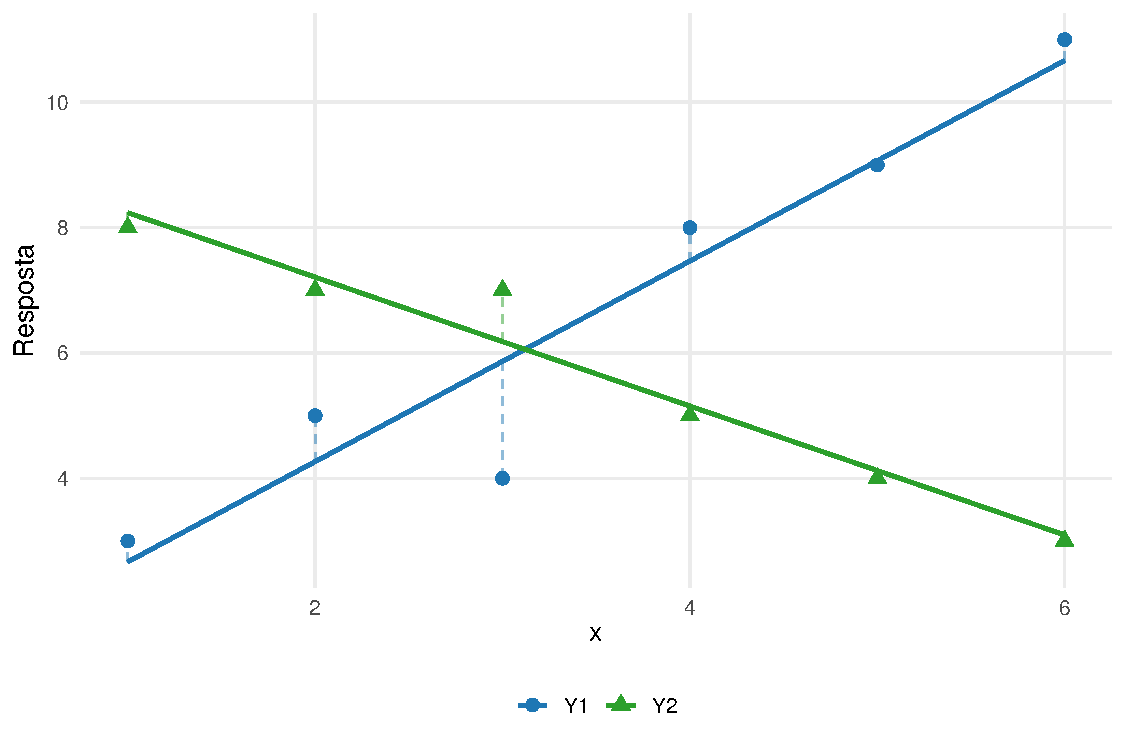
\includegraphics[keepaspectratio]{mod_2_modelo_files/figure-pdf/fig-exemplo-regressao-multivariada-ajuste-1.pdf}}

}

\caption{\label{fig-exemplo-regressao-multivariada-ajuste}Respostas
observadas, ajustes lineares e resíduos do exemplo integrado.}

\end{figure}%

A figura evidencia as inclinações em sentidos opostos das duas
respostas. Os segmentos tracejados ligam cada observação ao valor
ajustado correspondente e representam graficamente os resíduos que serão
reunidos na matriz \(\widehat{\mathbf U}\).

A matriz de valores ajustados é

\begin{equation}\phantomsection\label{eq-exemplo-regressao-multivariada-ajustes}{
\widehat{\mathbf Y}
=
\mathbf Z
\widehat{\mathbf B}_{\mathrm{obs}}
\approx
\begin{bmatrix}
2,667 & 8,238\\
4,267 & 7,210\\
5,867 & 6,181\\
7,467 & 5,152\\
9,067 & 4,124\\
10,667 & 3,095
\end{bmatrix}.
}\end{equation}

Consequentemente,

\begin{equation}\phantomsection\label{eq-exemplo-regressao-multivariada-residuos}{
\widehat{\mathbf U}
=
\mathbf Y
-
\widehat{\mathbf Y}
\approx
\begin{bmatrix}
0,333 & -0,238\\
0,733 & -0,210\\
-1,867 & 0,819\\
0,533 & -0,152\\
-0,067 & -0,124\\
0,333 & -0,095
\end{bmatrix}.
}\end{equation}

As equações normais garantem

\[
\mathbf Z^\top
\widehat{\mathbf U}
=
\mathbf0.
\]

Em particular, como o modelo contém intercepto, os resíduos somam zero
em cada resposta.

\textbf{SQPC residual e covariância residual}

A SQPC residual é

\begin{equation}\phantomsection\label{eq-exemplo-regressao-multivariada-sscp-residual}{
\begin{aligned}
\mathbf E
&=
\widehat{\mathbf U}^\top
\widehat{\mathbf U}
\\
&=
\begin{bmatrix}
68/15 & -28/15\\
-28/15 & 86/105
\end{bmatrix}
\\
&\approx
\begin{bmatrix}
4,533 & -1,867\\
-1,867 & 0,819
\end{bmatrix}.
\end{aligned}
}\end{equation}

Como

\[
n=6
\]

e

\[
r=2,
\]

os graus de liberdade residuais são

\[
\nu_E
=
n-r
=
4.
\]

A estimativa não viesada da matriz de covariâncias residual é

\begin{equation}\phantomsection\label{eq-exemplo-regressao-multivariada-covariancia-residual}{
\begin{aligned}
\widehat{\boldsymbol{\Sigma}}_{\mathrm{obs}}
&=
\frac{\mathbf E}{4}
\\
&=
\begin{bmatrix}
17/15 & -7/15\\
-7/15 & 43/210
\end{bmatrix}
\\
&\approx
\begin{bmatrix}
1,133 & -0,467\\
-0,467 & 0,205
\end{bmatrix}.
\end{aligned}
}\end{equation}

A covariância residual estimada é negativa. Isso indica que, depois de
removida a relação linear com \(x\), desvios positivos de uma resposta
tendem a ocorrer juntamente com desvios negativos da outra neste
conjunto de dados.

Sob o modelo normal matricial, como \(\mathbf E\succ\mathbf0\), a
estimativa de máxima verossimilhança é

\begin{equation}\phantomsection\label{eq-exemplo-regressao-multivariada-covariancia-mv}{
\begin{aligned}
\widehat{\boldsymbol{\Sigma}}_{\mathrm{MV,obs}}
&=
\frac{\mathbf E}{6}
\\
&\approx
\begin{bmatrix}
0,756 & -0,311\\
-0,311 & 0,137
\end{bmatrix}.
\end{aligned}
}\end{equation}

A diferença entre as duas estimativas decorre dos divisores:

\[
n-r=4
\]

para o estimador não viesado e

\[
n=6
\]

para a máxima verossimilhança sob normalidade.

\textbf{Decomposição da SQPC total}

Como o modelo contém intercepto,

\[
\mathbf T
=
\mathbf T_{\mathrm{mod}}
+
\mathbf E.
\]

A SQPC total é

\begin{equation}\phantomsection\label{eq-exemplo-regressao-multivariada-sscp-total}{
\mathbf T
=
\begin{bmatrix}
148/3 & -92/3\\
-92/3 & 58/3
\end{bmatrix}
\approx
\begin{bmatrix}
49,333 & -30,667\\
-30,667 & 19,333
\end{bmatrix}.
}\end{equation}

A parcela associada à covariável, além do intercepto, é

\begin{equation}\phantomsection\label{eq-exemplo-regressao-multivariada-sscp-modelo}{
\mathbf T_{\mathrm{mod}}
=
\begin{bmatrix}
224/5 & -144/5\\
-144/5 & 648/35
\end{bmatrix}
\approx
\begin{bmatrix}
44,800 & -28,800\\
-28,800 & 18,514
\end{bmatrix}.
}\end{equation}

Utilizando os valores exatos das matrizes,

\[
\mathbf T
=
\mathbf T_{\mathrm{mod}}
+
\mathbf E.
\]

Assim, a dispersão total em torno da média é decomposta na parcela
associada à covariável e na parcela residual.

Os graus de liberdade apresentam a decomposição correspondente:

\[
5
=
1
+
4,
\]

isto é,

\[
n-1
=
(r-1)
+
(n-r).
\]

\textbf{Hipótese sobre o efeito da covariável}

Considere a hipótese de que \(x\) não apresenta efeito linear sobre
nenhuma das duas respostas.

Para selecionar a segunda linha de \(\mathbf B\), defina

\[
\mathbf C_1
=
\begin{bmatrix}
0 & 1
\end{bmatrix}.
\]

Como as duas respostas são mantidas,

\[
\mathbf C_2
=
\mathbf I_2.
\]

A hipótese é

\[
H_0:
\mathbf C_1
\mathbf B
=
\mathbf0^\top,
\]

ou, equivalentemente,

\begin{equation}\phantomsection\label{eq-exemplo-regressao-multivariada-hipotese-inclinacoes}{
H_0:
\beta_{11}
=
\beta_{12}
=
0.
}\end{equation}

O afastamento observado em relação à hipótese nula é

\begin{equation}\phantomsection\label{eq-exemplo-regressao-multivariada-delta}{
\widehat{\boldsymbol{\Delta}}
=
\mathbf C_1
\widehat{\mathbf B}_{\mathrm{obs}}
=
\begin{bmatrix}
8/5 & -36/35
\end{bmatrix}
\approx
\begin{bmatrix}
1,600 & -1,029
\end{bmatrix}.
}\end{equation}

Nesse caso, \(\widehat{\boldsymbol{\Delta}}\) é exatamente o vetor
formado pelas duas inclinações estimadas, pois a hipótese especifica que
ambas devem ser iguais a zero.

A matriz associada à variabilidade desse contraste é escalar:

\begin{equation}\phantomsection\label{eq-exemplo-regressao-multivariada-gc}{
\begin{aligned}
\mathbf V_{C_1}
&=
\mathbf C_1
\left(
\mathbf Z^\top
\mathbf Z
\right)^{-1}
\mathbf C_1^\top
\\
&=
\frac{2}{35}
\\
&\approx
0,057.
\end{aligned}
}\end{equation}

A SQPC da hipótese é

\begin{equation}\phantomsection\label{eq-exemplo-regressao-multivariada-sscp-hipotese}{
\begin{aligned}
\mathbf H
&=
\widehat{\boldsymbol{\Delta}}^\top
\mathbf V_{C_1}^{-1}
\widehat{\boldsymbol{\Delta}}
\\
&=
\begin{bmatrix}
224/5 & -144/5\\
-144/5 & 648/35
\end{bmatrix}
\\
&\approx
\begin{bmatrix}
44,800 & -28,800\\
-28,800 & 18,514
\end{bmatrix}.
\end{aligned}
}\end{equation}

Nesse caso,

\[
\mathbf H
=
\mathbf T_{\mathrm{mod}}.
\]

O modelo completo contém intercepto e covariável, enquanto o modelo sob
\(H_0\) contém apenas o intercepto. Portanto, \(\mathbf H\) representa
exatamente a redução da SQPC residual obtida pela inclusão da
covariável.

Como o modelo reduzido contém somente a média geral,

\[
\mathbf E_R
=
\mathbf T,
\]

e

\[
\mathbf E_R
=
\mathbf H
+
\mathbf E.
\]

Assim, a hipótese sobre a covariável produz o par

\[
\left(
\mathbf H,
\mathbf E
\right),
\]

formado pela variação associada ao efeito examinado e pela variação
residual.

A decisão inferencial sobre essa hipótese será construída no Capítulo
12.

\textbf{Hipótese sobre uma combinação das respostas}

A mesma estrutura permite avaliar o efeito da covariável sobre uma
combinação específica das respostas.

Considere

\[
\mathbf c_2
=
\begin{bmatrix}
1\\
-1
\end{bmatrix}.
\]

A resposta transformada é

\[
Y_1-Y_2.
\]

A hipótese

\begin{equation}\phantomsection\label{eq-exemplo-regressao-multivariada-hipotese-bilateral}{
H_0:
\mathbf C_1
\mathbf B
\mathbf c_2
=
0
}\end{equation}

afirma que a covariável não apresenta efeito sobre a diferença entre as
duas respostas.

A estimativa é

\[
\begin{aligned}
\widehat{\theta}
&=
\mathbf C_1
\widehat{\mathbf B}_{\mathrm{obs}}
\mathbf c_2
\\
&=
\frac{92}{35}
\\
&\approx
2,629.
\end{aligned}
\]

Como

\[
V_{C_1}
=
\frac{2}{35},
\]

a SQPC da hipótese para essa combinação de respostas é o escalar

\[
\begin{aligned}
H_{c_2}
&=
\frac{
\widehat{\theta}^{\,2}
}{
V_{C_1}
}
\\
&=
\frac{4232}{35}
\\
&\approx
120,914.
\end{aligned}
\]

A SQPC residual dessa resposta transformada é

\begin{equation}\phantomsection\label{eq-exemplo-regressao-multivariada-sscp-resposta-transformada}{
\begin{aligned}
E_{c_2}
&=
\mathbf c_2^\top
\mathbf E
\mathbf c_2
\\
&=
\frac{318}{35}
\\
&\approx
9,086.
\end{aligned}
}\end{equation}

A hipótese sobre a diferença \(Y_1-Y_2\) produz, portanto, o par escalar

\[
\left(
H_{c_2},
E_{c_2}
\right)
=
\left(
\frac{4232}{35},
\frac{318}{35}
\right).
\]

O exemplo mostra duas formas de utilizar o mesmo ajuste. Com
\(\mathbf C_2=\mathbf I_2\), examina-se simultaneamente o efeito da
covariável nas duas respostas. Com

\[
\mathbf c_2
=
\begin{bmatrix}
1\\
-1
\end{bmatrix},
\]

examina-se o efeito da covariável sobre a diferença entre elas.

A construção das estatísticas de teste a partir desses pares pertence
aos capítulos posteriores.

Neste exemplo, uma única matriz de delineamento produziu sucessivamente

\[
\widehat{\mathbf B}_{\mathrm{obs}},
\qquad
\widehat{\mathbf Y},
\qquad
\widehat{\mathbf U},
\qquad
\mathbf E,
\qquad
\widehat{\boldsymbol{\Sigma}}_{\mathrm{obs}}
\]

e as matrizes associadas às hipóteses examinadas. No modelo de grupos
desenvolvido anteriormente, a mesma estrutura produz

\[
\mathbf E
=
\mathbf T_{\mathrm{intra}}
\]

e

\[
\mathbf H
=
\mathbf T_{\mathrm{entre}}
\]

quando a hipótese compara os vetores de médias dos grupos. Essa
correspondência será utilizada posteriormente na MANOVA e na Análise
Discriminante.

\end{example}

\section{Síntese do capítulo}\label{suxedntese-do-capuxedtulo-10}

O modelo linear multivariado representa conjuntamente \(p\) respostas
observadas nas mesmas \(n\) unidades:

\[
\boldsymbol{\mathcal Y}
=
\mathbf Z\mathbf B
+
\boldsymbol{\mathcal E}.
\]

A matriz \(\mathbf Z\) contém os \(q\) termos do modelo, \(\mathbf B\)
determina seus efeitos sobre as \(p\) respostas e

\[
E
\left(
\boldsymbol{\mathcal Y}
\mid
\mathbf Z
\right)
=
\mathbf Z\mathbf B
\]

é a estrutura de médias condicionais. A matriz

\[
\boldsymbol{\Sigma}
\]

descreve a covariância residual entre as respostas de uma mesma unidade.

Quando \(\mathbf Z\) possui posto coluna completo, a matriz de
parâmetros é estimada por

\[
\widehat{\mathbf B}
=
\left(
\mathbf Z^\top
\mathbf Z
\right)^{-1}
\mathbf Z^\top
\boldsymbol{\mathcal Y}.
\]

O ajuste depende do espaço coluna de \(\mathbf Z\). Os valores ajustados
e os resíduos são

\[
\widehat{\boldsymbol{\mathcal Y}}
=
\mathbf P_Z
\boldsymbol{\mathcal Y}
\]

e

\[
\widehat{\boldsymbol{\mathcal U}}
=
\mathbf M_Z
\boldsymbol{\mathcal Y},
\]

com

\[
\mathbf P_Z
+
\mathbf M_Z
=
\mathbf I_n.
\]

Assim, cada resposta é decomposta em uma parcela pertencente ao espaço
do modelo e uma parcela residual.

A SQPC residual

\[
\boldsymbol{\mathsf E}_{\mathrm{res}}
=
\widehat{\boldsymbol{\mathcal U}}^\top
\widehat{\boldsymbol{\mathcal U}}
\]

satisfaz

\[
E
\left(
\boldsymbol{\mathsf E}_{\mathrm{res}}
\mid
\mathbf Z
\right)
=
(n-r)
\boldsymbol{\Sigma},
\]

em que

\[
r
=
\operatorname{posto}
\left(
\mathbf Z
\right).
\]

Assim,

\[
\widehat{\boldsymbol{\Sigma}}
=
\frac{
\boldsymbol{\mathsf E}_{\mathrm{res}}
}{
n-r
}
\]

é um estimador não viesado da matriz de covariâncias residual.

Quando

\[
\mathbf1_n
\in
\mathcal C
\left(
\mathbf Z
\right),
\]

a dispersão em torno da média geral satisfaz

\[
\mathbf T
=
\mathbf T_{\mathrm{mod}}
+
\mathbf E,
\]

com graus de liberdade

\[
n-1
=
(r-1)
+
(n-r).
\]

No modelo de grupos,

\[
\mathbf E
=
\mathbf T_{\mathrm{intra}}
\]

e

\[
\mathbf T_{\mathrm{mod}}
=
\mathbf T_{\mathrm{entre}},
\]

de modo que

\[
\mathbf T
=
\mathbf T_{\mathrm{entre}}
+
\mathbf T_{\mathrm{intra}}.
\]

Assim, Proposição~\ref{prp-decomposicao-dispersao-grupos} passa a ser
representada como um caso particular da decomposição de um modelo de
médias. Essa correspondência fornece a estrutura matricial utilizada
posteriormente na ANOVA/MANOVA e na Análise Discriminante.

Quando

\[
\operatorname{posto}
\left(
\mathbf Z
\right)
<
q,
\]

os coeficientes podem não ser únicos, embora os valores ajustados e os
resíduos permaneçam determinados pelo espaço coluna de \(\mathbf Z\). As
comparações de interesse devem então ser formuladas por funções
estimáveis, como

\[
\mathbf C\mathbf B,
\]

com

\[
\mathbf C
=
\mathbf C
\mathbf Z^+
\mathbf Z.
\]

A hipótese linear multivariada geral é

\[
H_0:
\mathbf C_1
\mathbf B
\mathbf C_2
=
\boldsymbol{\Theta}_0.
\]

A matriz \(\mathbf C_1\) combina termos do modelo e \(\mathbf C_2\)
combina respostas. A hipótese produz duas matrizes construídas sobre as
mesmas combinações de respostas:

\[
\mathbf H
=
\widehat{\boldsymbol{\Delta}}^\top
\mathbf V_{C_1}^{-1}
\widehat{\boldsymbol{\Delta}}
\]

e

\[
\mathbf E_{C_2}
=
\mathbf C_2^\top
\mathbf E
\mathbf C_2.
\]

A primeira representa a variação associada ao afastamento da hipótese; a
segunda representa a variação residual correspondente. Quando
\(\mathbf C_2=\mathbf I_p\), obtém-se o par

\[
\left(
\mathbf H,
\mathbf E
\right),
\]

que será utilizado posteriormente na MANOVA.

A Tabela Tabela~\ref{tbl-sintese-modelo-linear-multivariado} reúne os
principais objetos utilizados no capítulo.

\begin{longtable}[]{@{}
  >{\raggedright\arraybackslash}p{(\linewidth - 4\tabcolsep) * \real{0.3333}}
  >{\raggedright\arraybackslash}p{(\linewidth - 4\tabcolsep) * \real{0.3333}}
  >{\raggedright\arraybackslash}p{(\linewidth - 4\tabcolsep) * \real{0.3333}}@{}}
\caption{Principais objetos do modelo linear
multivariado.}\label{tbl-sintese-modelo-linear-multivariado}\tabularnewline
\toprule\noalign{}
\begin{minipage}[b]{\linewidth}\raggedright
Objeto
\end{minipage} & \begin{minipage}[b]{\linewidth}\raggedright
Expressão
\end{minipage} & \begin{minipage}[b]{\linewidth}\raggedright
Papel
\end{minipage} \\
\midrule\noalign{}
\endfirsthead
\toprule\noalign{}
\begin{minipage}[b]{\linewidth}\raggedright
Objeto
\end{minipage} & \begin{minipage}[b]{\linewidth}\raggedright
Expressão
\end{minipage} & \begin{minipage}[b]{\linewidth}\raggedright
Papel
\end{minipage} \\
\midrule\noalign{}
\endhead
\bottomrule\noalign{}
\endlastfoot
estrutura de médias & \(\mathbf Z\mathbf B\) & determina os vetores de
médias permitidos pelo modelo \\
estimador dos parâmetros & \(\widehat{\mathbf B}\) & estima os
coeficientes associados aos termos e às respostas \\
projetor do modelo & \(\mathbf P_Z\) & produz os valores ajustados \\
projetor residual & \(\mathbf M_Z\) & produz os resíduos \\
SQPC residual & \(\mathbf E\) & representa a variação que permanece após
o ajuste \\
SQPC do modelo & \(\mathbf T_{\mathrm{mod}}\) & representa a dispersão
dos valores ajustados em torno da média geral \\
modelo de grupos & \(\mathbf E=\mathbf T_{\mathrm{intra}}\),
\(\mathbf T_{\mathrm{mod}}=\mathbf T_{\mathrm{entre}}\) & relaciona o
modelo linear à decomposição intra e entre grupos \\
função estimável & \(\mathbf C\mathbf B\) & representa comparações
determinadas pelo modelo \\
hipótese geral &
\(\mathbf C_1\mathbf B\mathbf C_2=\boldsymbol{\Theta}_0\) & combina
termos do modelo e respostas \\
SQPC da hipótese & \(\mathbf H\) & representa a variação associada ao
afastamento da hipótese \\
\end{longtable}

Ao concluir este capítulo, o estudante deve ser capaz de:

\begin{itemize}
\tightlist
\item
  formular um modelo linear para várias respostas e interpretar
  \(\mathbf Z\), \(\mathbf B\) e \(\boldsymbol{\Sigma}\);
\item
  obter valores ajustados e resíduos por meio das projeções associadas a
  \(\mathbf Z\);
\item
  construir a SQPC residual e estimar a matriz de covariâncias dos
  erros;
\item
  decompor a dispersão total em parcelas associada ao modelo e residual;
\item
  relacionar, no modelo de grupos, as matrizes \(\mathbf H\) e
  \(\mathbf E\) às dispersões entre e dentro dos grupos;
\item
  distinguir unicidade dos coeficientes de estimabilidade de combinações
  dos parâmetros;
\item
  interpretar a função de \(\mathbf C_1\) e de \(\mathbf C_2\) em uma
  hipótese linear;
\item
  formular hipóteses na forma
  \(\mathbf C_1\mathbf B\mathbf C_2=\boldsymbol{\Theta}_0\) e construir
  as SQPCs correspondentes.
\end{itemize}

Este capítulo construiu os estimadores, as projeções e as matrizes SQPC
que representam a variação associada ao modelo, ao resíduo e às
hipóteses lineares. O Capítulo 12 desenvolverá as distribuições
amostrais desses objetos e mostrará como utilizá-los na construção de
testes e regiões de confiança no contexto multivariado.

\chapter{Inferência Multivariada}\label{inferuxeancia-multivariada}

Os capítulos anteriores construíram os objetos sobre os quais será
formulada a inferência multivariada. A matriz de covariâncias
populacional foi definida em
Definição~\ref{def-matriz-covariancias-populacional}, a distribuição
normal multivariada em Definição~\ref{def-normal-multivariada}, o vetor
de médias amostral e suas propriedades em
Proposição~\ref{prp-media-amostral-momentos}, e a matriz de covariâncias
amostral em Definição~\ref{def-matriz-covariancias-amostral-aleatoria}.
O modelo linear multivariado foi definido em
Definição~\ref{def-modelo-linear-multivariado} e sua hipótese linear
geral em Definição~\ref{def-hipotese-linear-geral-multivariada}.

O objetivo deste capítulo é obter distribuições amostrais para esses
objetos e utilizá-las na construção de testes de hipóteses e regiões de
confiança. A distribuição de Wishart descreverá as matrizes SQPC sob
normalidade, enquanto a estatística \(T^2\) de Hotelling permitirá
realizar inferência sobre vetores de médias quando a matriz de
covariâncias populacional é desconhecida.

Os resultados exatos serão desenvolvidos principalmente sob normalidade
multivariada. Resultados assintóticos serão utilizados quando a
distribuição exata não estiver disponível ou quando o objetivo for
descrever o comportamento limite das estatísticas. As duas situações
serão distinguidas porque dependem de condições diferentes.

O capítulo também obterá as distribuições dos estimadores e das matrizes
SQPC construídas no modelo linear multivariado. Esses resultados
encerram a base probabilística e inferencial do Módulo 2 e serão
utilizados na formulação das técnicas do Módulo 3.

\begin{tcolorbox}[enhanced jigsaw, colback=white, breakable, bottomrule=.15mm, left=2mm, arc=.35mm, rightrule=.15mm, colframe=quarto-callout-note-color-frame, toprule=.15mm, leftrule=.75mm, opacityback=0]

\vspace{-3mm}\textbf{Convenções de notação}\vspace{3mm}

Neste capítulo:

\begin{itemize}
\tightlist
\item
  \(\bar{\boldsymbol{\mathsf X}}\) representa o vetor de médias amostral
  como estatística aleatória e \(\bar{\mathbf x}\) sua realização
  observada;
\item
  \(\boldsymbol{\mathsf S}\) representa a matriz de covariâncias
  amostral como estatística aleatória e \(\mathbf S\) sua realização
  observada;
\item
  \(\boldsymbol{\mathsf T}\) representa a SQPC amostral aleatória e
  \(\mathbf T\) sua realização observada;
\item
  \(\boldsymbol{\mathsf W}\) representa uma matriz aleatória com
  distribuição de Wishart;
\item
  \(\boldsymbol{\mathsf E}_{\mathrm{res}}\) e \(\mathbf E\) representam,
  respectivamente, a SQPC residual aleatória e sua realização observada;
\item
  \(\boldsymbol{\mathsf H}\) e \(\mathbf H\) representam,
  respectivamente, a SQPC da hipótese aleatória e sua realização
  observada;
\item
  \(\mathbf Z\) continua representando a matriz de delineamento do
  modelo linear multivariado;
\item
  \(\mathbf C_1\) combina termos do modelo e \(\mathbf C_2\) combina
  respostas nas hipóteses lineares definidas no Capítulo 11;
\item
  \(\mathbf M_Z\) permanece reservada ao projetor residual;
\item
  \(\mathbf A\) será utilizada posteriormente para formular hipóteses
  lineares diretamente sobre o vetor de médias.
\end{itemize}

As convenções preservam a distinção entre objetos populacionais,
estatísticas aleatórias e realizações observadas estabelecida nos
capítulos anteriores.

\end{tcolorbox}

\section{Distribuições amostrais exatas e
assintóticas}\label{distribuiuxe7uxf5es-amostrais-exatas-e-assintuxf3ticas}

A inferência estatística utiliza a distribuição amostral de uma
estatística para quantificar sua variabilidade e calibrar procedimentos
como testes e regiões de confiança. Essa distribuição pode ser conhecida
exatamente sob um modelo probabilístico especificado ou aproximada por
seu comportamento limite quando o tamanho amostral cresce.

\begin{definition}[Resultados exatos e
assintóticos]\protect\hypertarget{def-resultados-exatos-assintoticos}{}\label{def-resultados-exatos-assintoticos}

Um \textbf{resultado exato} é válido para o tamanho amostral considerado
sem recorrer a um argumento limite. Quando o resultado é distribucional,
ele fornece a distribuição da estatística sob as hipóteses
probabilísticas especificadas.

Um \textbf{resultado assintótico} descreve o comportamento limite de uma
estatística quando o tamanho amostral tende ao infinito. Sua utilização
em amostras finitas constitui uma aproximação cuja qualidade depende das
condições do problema.

\end{definition}

Neste capítulo, os resultados exatos dependerão principalmente da
normalidade multivariada. Os resultados assintóticos considerarão, salvo
indicação em contrário, o regime

\begin{equation}\phantomsection\label{eq-regime-assintotico-classico}{
p
\text{ fixo}
\qquad\text{e}\qquad
n
\longrightarrow
\infty.
}\end{equation}

Essa distinção deve ser mantida também na interpretação: uma
distribuição exata decorre do modelo probabilístico especificado,
enquanto uma distribuição limite decorre de um argumento de
convergência.

\subsection{Distribuição da média amostral sob
normalidade}\label{distribuiuxe7uxe3o-da-muxe9dia-amostral-sob-normalidade}

Considere uma amostra aleatória

\[
\boldsymbol{\mathsf X}_1,
\ldots,
\boldsymbol{\mathsf X}_n
\in
\mathbb R^p,
\]

independente e identicamente distribuída, com

\[
E
\left(
\boldsymbol{\mathsf X}_i
\right)
=
\boldsymbol{\mu}
\]

e

\[
\operatorname{Cov}
\left(
\boldsymbol{\mathsf X}_i
\right)
=
\boldsymbol{\Sigma}.
\]

O vetor de médias amostral é

\[
\bar{\boldsymbol{\mathsf X}}
=
\frac{1}{n}
\sum_{i=1}^{n}
\boldsymbol{\mathsf X}_i.
\]

Por Proposição~\ref{prp-media-amostral-momentos},

\[
E
\left(
\bar{\boldsymbol{\mathsf X}}
\right)
=
\boldsymbol{\mu}
\]

e

\[
\operatorname{Cov}
\left(
\bar{\boldsymbol{\mathsf X}}
\right)
=
\frac{\boldsymbol{\Sigma}}{n}.
\]

Esses resultados dependem dos momentos correspondentes, mas não da
normalidade multivariada.

A normalidade acrescenta a distribuição exata da estatística.

\begin{proposition}[Distribuição da média amostral sob
normalidade]\protect\hypertarget{prp-distribuicao-media-amostral-normal}{}\label{prp-distribuicao-media-amostral-normal}

Se

\[
\boldsymbol{\mathsf X}_1,
\ldots,
\boldsymbol{\mathsf X}_n
\stackrel{\mathrm{iid}}{\sim}
N_p
\left(
\boldsymbol{\mu},
\boldsymbol{\Sigma}
\right),
\]

então

\begin{equation}\phantomsection\label{eq-distribuicao-media-amostral-normal}{
\bar{\boldsymbol{\mathsf X}}
\sim
N_p
\left(
\boldsymbol{\mu},
\frac{\boldsymbol{\Sigma}}{n}
\right).
}\end{equation}

O resultado é exato para qualquer \(n\geq1\).

\end{proposition}

\begin{proof}
A média amostral é uma combinação linear dos vetores normais
independentes. Por Proposição~\ref{prp-transformacao-afim-normal}, sua
distribuição é normal multivariada.

Como Proposição~\ref{prp-media-amostral-momentos} fornece

\[
E
\left(
\bar{\boldsymbol{\mathsf X}}
\right)
=
\boldsymbol{\mu}
\]

e

\[
\operatorname{Cov}
\left(
\bar{\boldsymbol{\mathsf X}}
\right)
=
\frac{\boldsymbol{\Sigma}}{n},
\]

obtém-se Equação~\ref{eq-distribuicao-media-amostral-normal}.
\end{proof}

A proposição mostra a diferença entre propriedades de um estimador e sua
distribuição amostral. A igualdade

\[
E
\left(
\bar{\boldsymbol{\mathsf X}}
\right)
=
\boldsymbol{\mu}
\]

expressa ausência de viés. Já

\[
\bar{\boldsymbol{\mathsf X}}
\sim
N_p
\left(
\boldsymbol{\mu},
\frac{\boldsymbol{\Sigma}}{n}
\right)
\]

descreve toda a distribuição da estatística sob o modelo normal.

Se

\[
\boldsymbol{\Sigma}
\succ
\mathbf0,
\]

a média amostral pode ser branqueada:

\begin{equation}\phantomsection\label{eq-padronizacao-media-amostral-normal}{
\sqrt n\,
\boldsymbol{\Sigma}^{-1/2}
\left(
\bar{\boldsymbol{\mathsf X}}
-
\boldsymbol{\mu}
\right)
\sim
N_p
\left(
\mathbf0,
\mathbf I_p
\right).
}\end{equation}

Aplicando o resultado qui-quadrado da distância de Mahalanobis
estabelecido em Proposição~\ref{prp-mahalanobis-qui-quadrado},

\begin{equation}\phantomsection\label{eq-quadratica-media-amostral-qui-quadrado}{
n
\left(
\bar{\boldsymbol{\mathsf X}}
-
\boldsymbol{\mu}
\right)^\top
\boldsymbol{\Sigma}^{-1}
\left(
\bar{\boldsymbol{\mathsf X}}
-
\boldsymbol{\mu}
\right)
\sim
\chi_p^2.
}\end{equation}

O fator \(n\) aparece porque

\[
\operatorname{Cov}
\left(
\bar{\boldsymbol{\mathsf X}}
\right)
=
\frac{\boldsymbol{\Sigma}}{n},
\]

de modo que

\[
\left(
\frac{\boldsymbol{\Sigma}}{n}
\right)^{-1}
=
n\boldsymbol{\Sigma}^{-1}.
\]

A expressão em Equação~\ref{eq-quadratica-media-amostral-qui-quadrado}
fornece a base do procedimento inferencial para o vetor de médias quando
\(\boldsymbol{\Sigma}\) é conhecida. O caso em que
\(\boldsymbol{\Sigma}\) precisa ser estimada exigirá a distribuição da
matriz de covariâncias amostral.

\subsection{Teorema Central do Limite
multivariado}\label{teorema-central-do-limite-multivariado}

Fora da família normal, a distribuição de

\[
\bar{\boldsymbol{\mathsf X}}
\]

depende da distribuição conjunta da população. Em dimensão fixa, o
Teorema Central do Limite multivariado fornece uma aproximação normal
sob condições mais gerais (Vaart, 1998).

\begin{theorem}[Teorema Central do Limite
multivariado]\protect\hypertarget{thm-tcl-multivariado}{}\label{thm-tcl-multivariado}

Considere, para dimensão fixa \(p\), vetores aleatórios independentes e
identicamente distribuídos

\[
\boldsymbol{\mathsf X}_1,
\ldots,
\boldsymbol{\mathsf X}_n
\in
\mathbb R^p,
\]

com

\[
E
\left(
\boldsymbol{\mathsf X}_i
\right)
=
\boldsymbol{\mu}
\]

e matriz de covariâncias finita

\[
\operatorname{Cov}
\left(
\boldsymbol{\mathsf X}_i
\right)
=
\boldsymbol{\Sigma}.
\]

Então,

\begin{equation}\phantomsection\label{eq-tcl-multivariado}{
\sqrt n
\left(
\bar{\boldsymbol{\mathsf X}}
-
\boldsymbol{\mu}
\right)
\xrightarrow{d}
N_p
\left(
\mathbf0,
\boldsymbol{\Sigma}
\right).
}\end{equation}

\end{theorem}

\begin{proof}
Para qualquer vetor fixo

\[
\mathbf a
\in
\mathbb R^p,
\]

considere

\[
\sqrt n\,
\mathbf a^\top
\left(
\bar{\boldsymbol{\mathsf X}}
-
\boldsymbol{\mu}
\right)
=
\frac{1}{\sqrt n}
\sum_{i=1}^{n}
\mathbf a^\top
\left(
\boldsymbol{\mathsf X}_i
-
\boldsymbol{\mu}
\right).
\]

As variáveis

\[
\mathbf a^\top
\boldsymbol{\mathsf X}_1,
\ldots,
\mathbf a^\top
\boldsymbol{\mathsf X}_n
\]

são independentes e identicamente distribuídas, com média

\[
\mathbf a^\top
\boldsymbol{\mu}
\]

e variância finita

\[
\mathbf a^\top
\boldsymbol{\Sigma}
\mathbf a.
\]

Pelo Teorema Central do Limite univariado,

\[
\sqrt n\,
\mathbf a^\top
\left(
\bar{\boldsymbol{\mathsf X}}
-
\boldsymbol{\mu}
\right)
\xrightarrow{d}
N
\left(
0,
\mathbf a^\top
\boldsymbol{\Sigma}
\mathbf a
\right).
\]

Como a convergência vale para todo vetor fixo \(\mathbf a\), o Teorema
de Cramér--Wold em Teorema~\ref{thm-cramer-wold} implica
Equação~\ref{eq-tcl-multivariado}.
\end{proof}

O resultado permite escrever, em sentido assintótico,

\begin{equation}\phantomsection\label{eq-aproximacao-normal-media-amostral}{
\bar{\boldsymbol{\mathsf X}}
\overset{a}{\sim}
N_p
\left(
\boldsymbol{\mu},
\frac{\boldsymbol{\Sigma}}{n}
\right).
}\end{equation}

A mesma expressão possui, portanto, dois significados distintos:

\[
\bar{\boldsymbol{\mathsf X}}
\sim
N_p
\left(
\boldsymbol{\mu},
\frac{\boldsymbol{\Sigma}}{n}
\right)
\]

é uma distribuição \textbf{exata} quando a população é normal
multivariada, enquanto

\[
\bar{\boldsymbol{\mathsf X}}
\overset{a}{\sim}
N_p
\left(
\boldsymbol{\mu},
\frac{\boldsymbol{\Sigma}}{n}
\right)
\]

é uma aproximação \textbf{assintótica} sob as condições do
Teorema~\ref{thm-tcl-multivariado}.

Se

\[
\boldsymbol{\Sigma}
\succ
\mathbf0,
\]

então

\begin{equation}\phantomsection\label{eq-tcl-padronizado-media-amostral}{
\sqrt n\,
\boldsymbol{\Sigma}^{-1/2}
\left(
\bar{\boldsymbol{\mathsf X}}
-
\boldsymbol{\mu}
\right)
\xrightarrow{d}
N_p
\left(
\mathbf0,
\mathbf I_p
\right),
}\end{equation}

e, pelo teorema da aplicação contínua,

\begin{equation}\phantomsection\label{eq-tcl-quadratica-media-amostral}{
n
\left(
\bar{\boldsymbol{\mathsf X}}
-
\boldsymbol{\mu}
\right)^\top
\boldsymbol{\Sigma}^{-1}
\left(
\bar{\boldsymbol{\mathsf X}}
-
\boldsymbol{\mu}
\right)
\xrightarrow{d}
\chi_p^2.
}\end{equation}

Assim, a mesma forma quadrática possui distribuição qui-quadrado exata
sob normalidade e distribuição limite qui-quadrado sob as condições do
TCL multivariado.

\begin{tcolorbox}[enhanced jigsaw, colback=white, breakable, bottomrule=.15mm, left=2mm, arc=.35mm, rightrule=.15mm, colframe=quarto-callout-caution-color-frame, toprule=.15mm, leftrule=.75mm, opacityback=0]

\vspace{-3mm}\textbf{Alcance da aproximação assintótica}\vspace{3mm}

O Teorema~\ref{thm-tcl-multivariado} considera dimensão \(p\) fixa e
exige a existência dos momentos de segunda ordem.

O resultado não justifica automaticamente a inferência clássica quando
há dependência entre unidades, inexistência de segundos momentos ou
crescimento de \(p\) juntamente com \(n\). Além disso, a substituição de
\(\boldsymbol{\Sigma}\) por uma matriz de covariâncias estimada introduz
outra fonte de aleatoriedade que precisa ser considerada separadamente.

\end{tcolorbox}

A distribuição da média amostral descreve a incerteza associada à
localização. Quando \(\boldsymbol{\Sigma}\) é desconhecida, a inferência
depende também da distribuição da matriz que estima a dispersão. Sob
normalidade multivariada, essa distribuição é obtida a partir da
distribuição de Wishart.

\section{Distribuição de Wishart}\label{distribuiuxe7uxe3o-de-wishart}

A inferência sobre uma matriz de covariâncias exige conhecer a
distribuição das matrizes de produtos cruzados que a originam. No caso
univariado, somas de quadrados de variáveis normais padronizadas
conduzem à distribuição qui-quadrado. A distribuição de Wishart estende
essa construção para somas de produtos externos de vetores normais e
ocupa, na inferência normal multivariada, papel análogo ao da
distribuição qui-quadrado na inferência univariada (Muirhead, 1982).

\subsection{Construção e
parametrização}\label{construuxe7uxe3o-e-parametrizauxe7uxe3o}

Considere vetores aleatórios independentes

\[
\boldsymbol{\mathsf U}_1,
\ldots,
\boldsymbol{\mathsf U}_{\nu}
\in
\mathbb R^p
\]

tais que

\[
\boldsymbol{\mathsf U}_j
\sim
N_p
\left(
\mathbf0,
\boldsymbol{\Sigma}
\right),
\qquad
j=1,\ldots,\nu,
\]

com

\[
\nu
\in
\{1,2,\ldots\}
\]

e

\[
\boldsymbol{\Sigma}
\succ
\mathbf0.
\]

Cada produto externo

\[
\boldsymbol{\mathsf U}_j
\boldsymbol{\mathsf U}_j^\top
\]

é uma matriz simétrica e positiva semidefinida.

\begin{definition}[Distribuição de
Wishart]\protect\hypertarget{def-distribuicao-wishart}{}\label{def-distribuicao-wishart}

Se

\[
\boldsymbol{\mathsf U}_1,
\ldots,
\boldsymbol{\mathsf U}_{\nu}
\stackrel{\mathrm{iid}}{\sim}
N_p
\left(
\mathbf0,
\boldsymbol{\Sigma}
\right),
\]

com

\[
\nu
\in
\{1,2,\ldots\}
\]

e

\[
\boldsymbol{\Sigma}
\succ
\mathbf0,
\]

então a matriz aleatória

\begin{equation}\phantomsection\label{eq-construcao-distribuicao-wishart}{
\boldsymbol{\mathsf W}
=
\sum_{j=1}^{\nu}
\boldsymbol{\mathsf U}_j
\boldsymbol{\mathsf U}_j^\top
}\end{equation}

segue uma distribuição de Wishart com \(\nu\) graus de liberdade e
matriz de escala \(\boldsymbol{\Sigma}\).

Escreve-se

\begin{equation}\phantomsection\label{eq-notacao-distribuicao-wishart}{
\boldsymbol{\mathsf W}
\sim
W_p
\left(
\nu,
\boldsymbol{\Sigma}
\right).
}\end{equation}

\end{definition}

Nesta parametrização,

\[
\boldsymbol{\Sigma}
\]

é denominada \textbf{matriz de escala} e \(\nu\) é o número de graus de
liberdade. A relação

\[
E
\left(
\boldsymbol{\mathsf W}
\right)
=
\nu
\boldsymbol{\Sigma}
\]

será estabelecida em Proposição~\ref{prp-momentos-matriz-wishart}.

A parametrização é indicada explicitamente porque diferentes convenções
para a matriz de escala podem ser encontradas na literatura.

Quando

\[
p=1,
\]

a matriz Wishart possui um único elemento. Se

\[
\boldsymbol{\Sigma}
=
\begin{bmatrix}
\sigma^2
\end{bmatrix},
\]

então

\[
\mathsf W
=
\sum_{j=1}^{\nu}
\mathsf U_j^2
\]

e

\begin{equation}\phantomsection\label{eq-wishart-reducao-qui-quadrado}{
\frac{\mathsf W}{\sigma^2}
\sim
\chi_\nu^2.
}\end{equation}

Assim, a distribuição qui-quadrado é o caso univariado da distribuição
de Wishart.

\subsection{Suporte, posto e definição
positiva}\label{suporte-posto-e-definiuxe7uxe3o-positiva}

Organize os vetores geradores nas linhas da matriz

\[
\boldsymbol{\mathcal U}
=
\begin{bmatrix}
\boldsymbol{\mathsf U}_1^\top\\
\vdots\\
\boldsymbol{\mathsf U}_{\nu}^\top
\end{bmatrix}
\in
\mathbb R^{\nu\times p}.
\]

Então,

\begin{equation}\phantomsection\label{eq-wishart-matriz-gram}{
\boldsymbol{\mathsf W}
=
\boldsymbol{\mathcal U}^\top
\boldsymbol{\mathcal U}.
}\end{equation}

Portanto, \(\boldsymbol{\mathsf W}\) é uma matriz de Gram no sentido de
Definição~\ref{def-matriz-gram}. Por
Proposição~\ref{prp-propriedades-matriz-gram},

\[
\boldsymbol{\mathsf W}
\succeq
\mathbf0
\]

e

\[
\operatorname{posto}
\left(
\boldsymbol{\mathsf W}
\right)
=
\operatorname{posto}
\left(
\boldsymbol{\mathcal U}
\right)
\leq
\min
\left(
\nu,p
\right).
\]

\begin{proposition}[Posto de uma matriz
Wishart]\protect\hypertarget{prp-posto-matriz-wishart}{}\label{prp-posto-matriz-wishart}

Se

\[
\boldsymbol{\mathsf W}
\sim
W_p
\left(
\nu,
\boldsymbol{\Sigma}
\right),
\]

pela construção em Definição~\ref{def-distribuicao-wishart}, com

\[
\boldsymbol{\Sigma}
\succ
\mathbf0,
\]

então, com probabilidade 1,

\begin{equation}\phantomsection\label{eq-posto-matriz-wishart}{
\operatorname{posto}
\left(
\boldsymbol{\mathsf W}
\right)
=
\min
\left(
\nu,p
\right).
}\end{equation}

Consequentemente:

\begin{itemize}
\tightlist
\item
  se \(\nu\geq p\), então \(\boldsymbol{\mathsf W}\succ\mathbf0\) com
  probabilidade 1;
\item
  se \(\nu<p\), então
  \(\operatorname{posto}(\boldsymbol{\mathsf W})=\nu\) com probabilidade
  1 e a matriz é singular.
\end{itemize}

\end{proposition}

Como \(\boldsymbol{\Sigma}\succ\mathbf0\), cada vetor gerador possui
distribuição normal não singular. A distribuição conjunta das entradas
de \(\boldsymbol{\mathcal U}\) é contínua, e o conjunto das matrizes
cujo posto é menor que \(\min(\nu,p)\) possui probabilidade zero. Assim,
a matriz de Gram atinge quase certamente o maior posto permitido por
suas dimensões (Muirhead, 1982).

A condição

\[
\nu\geq p
\]

é, portanto, necessária e suficiente para a definição positiva quase
certa na construção com graus de liberdade inteiros e

\[
\boldsymbol{\Sigma}\succ\mathbf0.
\]

\subsection{Momentos}\label{momentos}

A esperança da matriz Wishart é obtida diretamente da construção por
produtos externos.

\begin{proposition}[Momentos de uma matriz
Wishart]\protect\hypertarget{prp-momentos-matriz-wishart}{}\label{prp-momentos-matriz-wishart}

Se

\[
\boldsymbol{\mathsf W}
\sim
W_p
\left(
\nu,
\boldsymbol{\Sigma}
\right),
\]

pela construção em Definição~\ref{def-distribuicao-wishart}, então

\begin{equation}\phantomsection\label{eq-esperanca-matriz-wishart}{
E
\left(
\boldsymbol{\mathsf W}
\right)
=
\nu
\boldsymbol{\Sigma}.
}\end{equation}

Para os elementos da matriz,

\begin{equation}\phantomsection\label{eq-covariancia-elementos-wishart}{
\operatorname{Cov}
\left(
\mathsf W_{jk},
\mathsf W_{\ell m}
\right)
=
\nu
\left(
\sigma_{j\ell}\sigma_{km}
+
\sigma_{jm}\sigma_{k\ell}
\right).
}\end{equation}

\end{proposition}

\begin{proof}
Pela construção em Equação~\ref{eq-construcao-distribuicao-wishart},

\[
\mathsf W_{jk}
=
\sum_{h=1}^{\nu}
\mathsf U_{hj}
\mathsf U_{hk}.
\]

Como

\[
E
\left(
\mathsf U_{hj}
\mathsf U_{hk}
\right)
=
\sigma_{jk},
\]

segue que

\[
E
\left(
\mathsf W_{jk}
\right)
=
\nu\sigma_{jk}.
\]

Portanto,

\[
E
\left(
\boldsymbol{\mathsf W}
\right)
=
\nu
\boldsymbol{\Sigma}.
\]

A expressão para

\[
\operatorname{Cov}
\left(
\mathsf W_{jk},
\mathsf W_{\ell m}
\right)
\]

decorre dos momentos de quarta ordem do vetor normal de média zero e da
independência entre os \(\nu\) vetores geradores (Muirhead, 1982).
\end{proof}

Em particular,

\begin{equation}\phantomsection\label{eq-variancia-diagonal-wishart}{
\operatorname{Var}
\left(
\mathsf W_{jj}
\right)
=
2\nu\sigma_{jj}^2,
}\end{equation}

e, para \(j\neq k\),

\begin{equation}\phantomsection\label{eq-variancia-fora-diagonal-wishart}{
\operatorname{Var}
\left(
\mathsf W_{jk}
\right)
=
\nu
\left(
\sigma_{jj}\sigma_{kk}
+
\sigma_{jk}^2
\right).
}\end{equation}

Dividindo pelos graus de liberdade,

\[
E
\left(
\frac{
\boldsymbol{\mathsf W}
}{
\nu
}
\right)
=
\boldsymbol{\Sigma}.
\]

Além disso, Equação~\ref{eq-covariancia-elementos-wishart} implica

\[
\operatorname{Cov}
\left(
\frac{\mathsf W_{jk}}{\nu},
\frac{\mathsf W_{\ell m}}{\nu}
\right)
=
\frac{
\sigma_{j\ell}\sigma_{km}
+
\sigma_{jm}\sigma_{k\ell}
}{
\nu
}.
\]

Portanto, para \(\boldsymbol{\Sigma}\) fixa, a variabilidade dos
elementos de \(\boldsymbol{\mathsf W}/\nu\) diminui à medida que \(\nu\)
aumenta.

\subsection{Formas quadráticas}\label{formas-quadruxe1ticas-1}

A analogia com a distribuição qui-quadrado também aparece em qualquer
direção fixa do espaço das variáveis.

\begin{proposition}[Forma quadrática de uma matriz
Wishart]\protect\hypertarget{prp-forma-quadratica-wishart}{}\label{prp-forma-quadratica-wishart}

Se

\[
\boldsymbol{\mathsf W}
\sim
W_p
\left(
\nu,
\boldsymbol{\Sigma}
\right)
\]

pela construção em Definição~\ref{def-distribuicao-wishart}, então, para
qualquer

\[
\mathbf a
\in
\mathbb R^p,
\qquad
\mathbf a\neq\mathbf0,
\]

vale

\begin{equation}\phantomsection\label{eq-forma-quadratica-wishart-qui-quadrado}{
\frac{
\mathbf a^\top
\boldsymbol{\mathsf W}
\mathbf a
}{
\mathbf a^\top
\boldsymbol{\Sigma}
\mathbf a
}
\sim
\chi_\nu^2.
}\end{equation}

\end{proposition}

\begin{proof}
De Equação~\ref{eq-construcao-distribuicao-wishart},

\[
\mathbf a^\top
\boldsymbol{\mathsf W}
\mathbf a
=
\sum_{j=1}^{\nu}
\left(
\mathbf a^\top
\boldsymbol{\mathsf U}_j
\right)^2.
\]

Por Proposição~\ref{prp-transformacao-afim-normal},

\[
\mathbf a^\top
\boldsymbol{\mathsf U}_j
\sim
N
\left(
0,
\mathbf a^\top
\boldsymbol{\Sigma}
\mathbf a
\right).
\]

Assim, as variáveis

\[
\frac{
\mathbf a^\top
\boldsymbol{\mathsf U}_j
}{
\sqrt{
\mathbf a^\top
\boldsymbol{\Sigma}
\mathbf a
}
}
\]

são normais padrão independentes. A soma de seus quadrados possui
distribuição \(\chi_\nu^2\).
\end{proof}

Assim, cada projeção univariada de uma matriz Wishart recupera a
estrutura qui-quadrado correspondente à variância naquela direção.

\subsection{Aditividade}\label{aditividade}

\begin{proposition}[Aditividade da distribuição de
Wishart]\protect\hypertarget{prp-aditividade-wishart}{}\label{prp-aditividade-wishart}

Se

\[
\boldsymbol{\mathsf W}_1
\sim
W_p
\left(
\nu_1,
\boldsymbol{\Sigma}
\right)
\]

e

\[
\boldsymbol{\mathsf W}_2
\sim
W_p
\left(
\nu_2,
\boldsymbol{\Sigma}
\right)
\]

são independentes e possuem a mesma matriz de escala, então

\begin{equation}\phantomsection\label{eq-aditividade-distribuicao-wishart}{
\boldsymbol{\mathsf W}_1
+
\boldsymbol{\mathsf W}_2
\sim
W_p
\left(
\nu_1+\nu_2,
\boldsymbol{\Sigma}
\right).
}\end{equation}

\end{proposition}

\begin{proof}
Pela construção da distribuição, as duas matrizes podem ser
representadas por somas de, respectivamente, \(\nu_1\) e \(\nu_2\)
produtos externos de vetores normais independentes com a mesma matriz de
covariâncias \(\boldsymbol{\Sigma}\).

A soma das duas matrizes reúne

\[
\nu_1+\nu_2
\]

produtos externos independentes e, portanto, possui a distribuição
indicada.
\end{proof}

A condição de escala comum é necessária para esse resultado. Matrizes
Wishart independentes com matrizes de escala distintas não podem, em
geral, ser somadas mantendo a mesma forma Wishart.

\subsection{Transformações
lineares}\label{transformauxe7uxf5es-lineares-1}

A transformação de uma matriz Wishart acompanha a transformação da
matriz de covariâncias dos vetores normais que a geram.

\begin{proposition}[Transformação linear de uma matriz
Wishart]\protect\hypertarget{prp-transformacao-linear-wishart}{}\label{prp-transformacao-linear-wishart}

Considere

\[
\boldsymbol{\mathsf W}
\sim
W_p
\left(
\nu,
\boldsymbol{\Sigma}
\right)
\]

pela construção em Definição~\ref{def-distribuicao-wishart}.

Se

\[
\mathbf L
\in
\mathbb R^{r\times p}
\]

possui posto linha completo,

\[
\operatorname{posto}
\left(
\mathbf L
\right)
=
r,
\]

então

\begin{equation}\phantomsection\label{eq-transformacao-linear-distribuicao-wishart}{
\mathbf L
\boldsymbol{\mathsf W}
\mathbf L^\top
\sim
W_r
\left(
\nu,
\mathbf L
\boldsymbol{\Sigma}
\mathbf L^\top
\right).
}\end{equation}

\end{proposition}

\begin{proof}
Pela construção,

\[
\begin{aligned}
\mathbf L
\boldsymbol{\mathsf W}
\mathbf L^\top
&=
\sum_{j=1}^{\nu}
\left(
\mathbf L
\boldsymbol{\mathsf U}_j
\right)
\left(
\mathbf L
\boldsymbol{\mathsf U}_j
\right)^\top.
\end{aligned}
\]

Por Proposição~\ref{prp-transformacao-afim-normal},

\[
\mathbf L
\boldsymbol{\mathsf U}_j
\sim
N_r
\left(
\mathbf0,
\mathbf L
\boldsymbol{\Sigma}
\mathbf L^\top
\right).
\]

Como as transformações são aplicadas separadamente aos vetores
independentes, os vetores transformados permanecem independentes.

Como \(\mathbf L\) possui posto linha completo e

\[
\boldsymbol{\Sigma}
\succ
\mathbf0,
\]

tem-se

\[
\mathbf L
\boldsymbol{\Sigma}
\mathbf L^\top
\succ
\mathbf0.
\]

Logo, a soma possui a distribuição apresentada.
\end{proof}

Se \(\mathbf L\) não possui posto linha completo,

\[
\mathbf L
\boldsymbol{\Sigma}
\mathbf L^\top
\]

é singular e a distribuição fica restrita ao subespaço imagem de
\(\mathbf L\). Essa extensão singular não será necessária na sequência
principal.

Tomando

\[
\mathbf L
=
\boldsymbol{\Sigma}^{-1/2},
\]

com a raiz quadrada principal definida em
Definição~\ref{def-raiz-quadrada-principal}, obtém-se

\begin{equation}\phantomsection\label{eq-padronizacao-matriz-wishart}{
\boldsymbol{\Sigma}^{-1/2}
\boldsymbol{\mathsf W}
\boldsymbol{\Sigma}^{-1/2}
\sim
W_p
\left(
\nu,
\mathbf I_p
\right).
}\end{equation}

A transformação remove a matriz de escala da distribuição, de modo
análogo ao branqueamento normal em
Equação~\ref{eq-branqueamento-normal}.

\subsection{Aprofundamento: densidade da distribuição de
Wishart}\label{aprofundamento-densidade-da-distribuiuxe7uxe3o-de-wishart}

\begin{tcolorbox}[enhanced jigsaw, colback=white, breakable, bottomrule=.15mm, left=2mm, arc=.35mm, rightrule=.15mm, colframe=quarto-callout-note-color-frame, toprule=.15mm, leftrule=.75mm, opacityback=0]

\vspace{-3mm}\textbf{Leitura de aprofundamento}\vspace{3mm}

Os resultados inferenciais deste capítulo utilizam principalmente a
construção por produtos externos, o posto, os momentos, a aditividade e
as transformações da distribuição de Wishart.

A densidade é apresentada como aprofundamento porque será útil para
relacionar a distribuição de Wishart a verossimilhanças envolvendo
matrizes de covariâncias.

\end{tcolorbox}

A construção em Definição~\ref{def-distribuicao-wishart} utiliza um
número inteiro de vetores normais. A família Wishart não singular admite
uma extensão para graus de liberdade reais

\[
\nu>p-1
\]

por meio de sua densidade no cone das matrizes simétricas positivas
definidas (Muirhead, 1982).

\begin{proposition}[Densidade da distribuição de
Wishart]\protect\hypertarget{prp-densidade-wishart}{}\label{prp-densidade-wishart}

Se

\[
\boldsymbol{\mathsf W}
\sim
W_p
\left(
\nu,
\boldsymbol{\Sigma}
\right),
\]

com

\[
\nu>p-1
\]

e

\[
\boldsymbol{\Sigma}
\succ
\mathbf0,
\]

então sua densidade é

\begin{equation}\phantomsection\label{eq-densidade-distribuicao-wishart}{
f_{\boldsymbol{\mathsf W}}
\left(
\mathbf W
\right)
=
\frac{
|\mathbf W|^{(\nu-p-1)/2}
\exp
\left[
-\frac12
\operatorname{tr}
\left(
\boldsymbol{\Sigma}^{-1}
\mathbf W
\right)
\right]
}{
2^{\nu p/2}
|\boldsymbol{\Sigma}|^{\nu/2}
\Gamma_p
\left(
\nu/2
\right)
},
}\end{equation}

para

\[
\mathbf W
\succ
\mathbf0.
\]

\end{proposition}

A função gama multivariada é

\begin{equation}\phantomsection\label{eq-funcao-gama-multivariada}{
\Gamma_p
\left(
a
\right)
=
\pi^{p(p-1)/4}
\prod_{j=1}^{p}
\Gamma
\left(
a-\frac{j-1}{2}
\right),
}\end{equation}

definida para

\[
a>
\frac{p-1}{2}.
\]

Quando a Wishart é construída pela soma de \(\nu\) produtos externos e

\[
\nu<p,
\]

a matriz é singular com probabilidade 1. Nesse caso, sua distribuição
está concentrada em matrizes positivas semidefinidas de posto \(\nu\) e
não possui a densidade anterior no cone positivo definido.

A sequência inferencial deste capítulo utilizará graus de liberdade
inteiros provenientes do tamanho amostral ou do posto de matrizes de
projeção.

\subsection{Distribuição da SQPC e da covariância
amostral}\label{distribuiuxe7uxe3o-da-sqpc-e-da-covariuxe2ncia-amostral}

Retomando Definição~\ref{def-sscp-amostral-aleatoria},

\[
\boldsymbol{\mathsf T}
=
\sum_{i=1}^{n}
\left(
\boldsymbol{\mathsf X}_i
-
\bar{\boldsymbol{\mathsf X}}
\right)
\left(
\boldsymbol{\mathsf X}_i
-
\bar{\boldsymbol{\mathsf X}}
\right)^\top.
\]

Por Definição~\ref{def-matriz-covariancias-amostral-aleatoria},

\[
\boldsymbol{\mathsf S}
=
\frac{
\boldsymbol{\mathsf T}
}{
n-1
}.
\]

Por Proposição~\ref{prp-esperanca-sscp-amostral},

\[
E
\left(
\boldsymbol{\mathsf T}
\right)
=
(n-1)
\boldsymbol{\Sigma}.
\]

Sob normalidade multivariada, a distribuição completa dessa estatística
pode ser estabelecida.

\begin{theorem}[Distribuição da SQPC e da covariância
amostral]\protect\hypertarget{thm-distribuicao-sscp-amostral-normal}{}\label{thm-distribuicao-sscp-amostral-normal}

Se

\[
\boldsymbol{\mathsf X}_1,
\ldots,
\boldsymbol{\mathsf X}_n
\stackrel{\mathrm{iid}}{\sim}
N_p
\left(
\boldsymbol{\mu},
\boldsymbol{\Sigma}
\right),
\]

com

\[
n\geq2
\]

e

\[
\boldsymbol{\Sigma}
\succ
\mathbf0,
\]

então

\begin{equation}\phantomsection\label{eq-distribuicao-sscp-amostral-wishart}{
\boldsymbol{\mathsf T}
=
(n-1)
\boldsymbol{\mathsf S}
\sim
W_p
\left(
n-1,
\boldsymbol{\Sigma}
\right).
}\end{equation}

\end{theorem}

\begin{proof}
Organize a amostra na matriz aleatória

\[
\boldsymbol{\mathcal X}
=
\begin{bmatrix}
\boldsymbol{\mathsf X}_1^\top\\
\vdots\\
\boldsymbol{\mathsf X}_n^\top
\end{bmatrix}.
\]

Considere uma matriz ortogonal

\[
\mathbf Q
\in
\mathbb R^{n\times n}
\]

cuja primeira linha seja

\[
\frac{1}{\sqrt n}
\mathbf1_n^\top,
\]

e defina a matriz transformada

\[
\boldsymbol{\mathcal X}^{\star}
=
\mathbf Q
\boldsymbol{\mathcal X}.
\]

Sua primeira linha satisfaz

\begin{equation}\phantomsection\label{eq-primeira-linha-transformacao-wishart-amostral}{
\left(
\boldsymbol{\mathsf X}_1^{\star}
\right)^\top
=
\sqrt n\,
\bar{\boldsymbol{\mathsf X}}^\top.
}\end{equation}

As demais linhas são combinações lineares cujos coeficientes somam zero.
Portanto,

\[
E
\left(
\boldsymbol{\mathsf X}_j^{\star}
\right)
=
\mathbf0,
\qquad
j=2,\ldots,n.
\]

A covariância cruzada entre duas linhas transformadas é

\[
\operatorname{Cov}
\left(
\boldsymbol{\mathsf X}_j^{\star},
\boldsymbol{\mathsf X}_k^{\star}
\right)
=
\left[
\mathbf Q
\mathbf Q^\top
\right]_{jk}
\boldsymbol{\Sigma}
=
\delta_{jk}
\boldsymbol{\Sigma}.
\]

As linhas transformadas são conjuntamente normais. Por
Proposição~\ref{prp-independencia-blocos-normais}, as covariâncias
cruzadas nulas implicam independência. Assim,

\[
\boldsymbol{\mathsf X}_2^{\star},
\ldots,
\boldsymbol{\mathsf X}_n^{\star}
\stackrel{\mathrm{iid}}{\sim}
N_p
\left(
\mathbf0,
\boldsymbol{\Sigma}
\right).
\]

A matriz de centralização pode ser escrita como

\[
\mathbf H_n
=
\mathbf Q^\top
\begin{bmatrix}
0 & \mathbf0^\top\\
\mathbf0 & \mathbf I_{n-1}
\end{bmatrix}
\mathbf Q.
\]

Utilizando a forma matricial da SQPC estabelecida em
Equação~\ref{eq-sscp-amostral-forma-matricial},

\[
\begin{aligned}
\boldsymbol{\mathsf T}
&=
\boldsymbol{\mathcal X}^\top
\mathbf H_n
\boldsymbol{\mathcal X}
\\
&=
\sum_{j=2}^{n}
\boldsymbol{\mathsf X}_j^{\star}
\left(
\boldsymbol{\mathsf X}_j^{\star}
\right)^\top.
\end{aligned}
\]

Essa é a soma de \(n-1\) produtos externos de vetores independentes com
distribuição

\[
N_p
\left(
\mathbf0,
\boldsymbol{\Sigma}
\right).
\]

Pela Definição~\ref{def-distribuicao-wishart},

\[
\boldsymbol{\mathsf T}
\sim
W_p
\left(
n-1,
\boldsymbol{\Sigma}
\right).
\]
\end{proof}

A esperança obtida pela distribuição de Wishart é consistente com
Proposição~\ref{prp-esperanca-sscp-amostral} e
Proposição~\ref{prp-nao-viesamento-covariancia-amostral}.

A informação nova é a distribuição amostral completa:

\[
(n-1)
\boldsymbol{\mathsf S}
\sim
W_p
\left(
n-1,
\boldsymbol{\Sigma}
\right).
\]

Pela Proposição~\ref{prp-forma-quadratica-wishart}, para qualquer

\[
\mathbf a
\neq
\mathbf0,
\]

tem-se

\begin{equation}\phantomsection\label{eq-distribuicao-variancia-amostral-direcao}{
\frac{
(n-1)
\mathbf a^\top
\boldsymbol{\mathsf S}
\mathbf a
}{
\mathbf a^\top
\boldsymbol{\Sigma}
\mathbf a
}
\sim
\chi_{n-1}^2.
}\end{equation}

Assim, a variância amostral de qualquer combinação linear fixa possui a
mesma estrutura qui-quadrado conhecida do caso univariado.

Para os elementos de \(\boldsymbol{\mathsf S}\),

\begin{equation}\phantomsection\label{eq-covariancia-elementos-covariancia-amostral-normal}{
\operatorname{Cov}
\left(
\mathsf S_{jk},
\mathsf S_{\ell m}
\right)
=
\frac{
\sigma_{j\ell}\sigma_{km}
+
\sigma_{jm}\sigma_{k\ell}
}{
n-1
}.
}\end{equation}

Em particular,

\[
\operatorname{Var}
\left(
\mathsf S_{jj}
\right)
=
\frac{
2\sigma_{jj}^2
}{
n-1
}
\]

e, para \(j\neq k\),

\[
\operatorname{Var}
\left(
\mathsf S_{jk}
\right)
=
\frac{
\sigma_{jj}\sigma_{kk}
+
\sigma_{jk}^2
}{
n-1
}.
\]

Esses resultados são exatos sob normalidade multivariada.

A matriz de covariâncias amostral possui, com probabilidade 1,

\begin{equation}\phantomsection\label{eq-posto-covariancia-amostral-normal}{
\operatorname{posto}
\left(
\boldsymbol{\mathsf S}
\right)
=
\min
\left(
p,n-1
\right).
}\end{equation}

Portanto, sob

\[
\boldsymbol{\Sigma}
\succ
\mathbf0,
\]

a condição

\begin{equation}\phantomsection\label{eq-condicao-inversao-covariancia-amostral}{
n>p
}\end{equation}

é necessária e suficiente para que

\[
\boldsymbol{\mathsf S}
\succ
\mathbf0
\]

com probabilidade 1.

Quando

\[
p\geq n,
\]

a matriz \(\boldsymbol{\mathsf S}\) é necessariamente singular. Essa
restrição dimensional terá consequência direta para a forma clássica da
estatística \(T^2\) de Hotelling.

Sob o modelo normal, Equação~\ref{eq-mv-covariancia-normal} fornece

\[
\widehat{\boldsymbol{\Sigma}}_{\mathrm{MV}}
=
\frac{
\boldsymbol{\mathsf T}
}{
n
}.
\]

Sempre que sua interpretação como estimador de máxima verossimilhança no
espaço

\[
\boldsymbol{\Sigma}
\succ
\mathbf0
\]

for válida,

\begin{equation}\phantomsection\label{eq-distribuicao-estimador-mv-covariancia-normal}{
n
\widehat{\boldsymbol{\Sigma}}_{\mathrm{MV}}
=
\boldsymbol{\mathsf T}
\sim
W_p
\left(
n-1,
\boldsymbol{\Sigma}
\right).
}\end{equation}

A distribuição continua envolvendo \(n-1\) graus de liberdade, pois a
média populacional também foi estimada a partir da amostra.

\subsection{Independência entre média e
covariância}\label{independuxeancia-entre-muxe9dia-e-covariuxe2ncia}

A transformação ortogonal utilizada na prova do
Teorema~\ref{thm-distribuicao-sscp-amostral-normal} separa a informação
amostral associada à localização da informação associada à dispersão.

A primeira linha transformada depende exclusivamente de

\[
\bar{\boldsymbol{\mathsf X}},
\]

enquanto

\[
\boldsymbol{\mathsf T}
\]

e, consequentemente,

\[
\boldsymbol{\mathsf S},
\]

dependem apenas das demais linhas.

\begin{theorem}[Independência entre média e covariância
amostral]\protect\hypertarget{thm-independencia-media-covariancia-normal}{}\label{thm-independencia-media-covariancia-normal}

Se

\[
\boldsymbol{\mathsf X}_1,
\ldots,
\boldsymbol{\mathsf X}_n
\stackrel{\mathrm{iid}}{\sim}
N_p
\left(
\boldsymbol{\mu},
\boldsymbol{\Sigma}
\right),
\]

com

\[
n\geq2
\]

e

\[
\boldsymbol{\Sigma}
\succ
\mathbf0,
\]

então

\[
\bar{\boldsymbol{\mathsf X}}
\perp
\boldsymbol{\mathsf T}.
\]

Como

\[
\boldsymbol{\mathsf S}
=
\frac{
\boldsymbol{\mathsf T}
}{
n-1
},
\]

também vale

\begin{equation}\phantomsection\label{eq-independencia-media-covariancia-normal}{
\bar{\boldsymbol{\mathsf X}}
\perp
\boldsymbol{\mathsf S}.
}\end{equation}

\end{theorem}

\begin{proof}
Na prova de Teorema~\ref{thm-distribuicao-sscp-amostral-normal}, a
primeira linha de \(\boldsymbol{\mathcal X}^{\star}\) depende apenas de

\[
\bar{\boldsymbol{\mathsf X}},
\]

enquanto \(\boldsymbol{\mathsf T}\) depende apenas das demais linhas
transformadas.

Esses dois blocos são independentes por
Proposição~\ref{prp-independencia-blocos-normais}. Portanto,

\[
\bar{\boldsymbol{\mathsf X}}
\perp
\boldsymbol{\mathsf T}.
\]

Como

\[
\boldsymbol{\mathsf S}
=
\frac{\boldsymbol{\mathsf T}}{n-1},
\]

segue também

\[
\bar{\boldsymbol{\mathsf X}}
\perp
\boldsymbol{\mathsf S}.
\]
\end{proof}

A independência é um resultado \textbf{exato da amostragem normal}. Ela
não decorre somente da independência entre as observações.

\begin{tcolorbox}[enhanced jigsaw, colback=white, breakable, bottomrule=.15mm, left=2mm, arc=.35mm, rightrule=.15mm, colframe=quarto-callout-caution-color-frame, toprule=.15mm, leftrule=.75mm, opacityback=0]

\vspace{-3mm}\textbf{O que depende da normalidade}\vspace{3mm}

As propriedades

\[
E
\left(
\bar{\boldsymbol{\mathsf X}}
\right)
=
\boldsymbol{\mu}
\]

e

\[
E
\left(
\boldsymbol{\mathsf S}
\right)
=
\boldsymbol{\Sigma}
\]

não exigem normalidade multivariada.

Em contraste,

\[
(n-1)
\boldsymbol{\mathsf S}
\sim
W_p
\left(
n-1,
\boldsymbol{\Sigma}
\right)
\]

e

\[
\bar{\boldsymbol{\mathsf X}}
\perp
\boldsymbol{\mathsf S}
\]

são resultados exatos da amostragem normal.

Para uma população geral, a distribuição de \(\boldsymbol{\mathsf S}\)
depende de características adicionais da distribuição, incluindo
momentos de ordem superior, e a média e a covariância amostrais não são,
em geral, independentes.

\end{tcolorbox}

Temos, portanto, sob amostragem normal, o par

\[
\bar{\boldsymbol{\mathsf X}}
\sim
N_p
\left(
\boldsymbol{\mu},
\frac{
\boldsymbol{\Sigma}
}{
n
}
\right)
\]

e

\[
(n-1)
\boldsymbol{\mathsf S}
\sim
W_p
\left(
n-1,
\boldsymbol{\Sigma}
\right),
\]

com

\begin{equation}\phantomsection\label{eq-estrutura-normal-wishart-amostra}{
\bar{\boldsymbol{\mathsf X}}
\perp
\boldsymbol{\mathsf S}.
}\end{equation}

O par

\[
\left(
\bar{\boldsymbol{\mathsf X}},
\boldsymbol{\mathsf S}
\right)
\]

combina uma distribuição normal para a localização, uma distribuição
Wishart para a dispersão e independência entre os dois objetos. Essa
estrutura normal--Wishart será utilizada posteriormente na construção da
estatística \(T^2\) de Hotelling.

No modelo linear multivariado, a mesma organização reaparece. O vetor de
médias amostral é substituído pelo estimador de \(\mathbf B\), enquanto
a SQPC amostral é substituída pela SQPC residual. Os \(n-1\) graus de
liberdade do problema de uma única média passam a ser os \(n-r\) graus
de liberdade residuais do modelo.

\section{Distribuições no modelo linear
multivariado}\label{distribuiuxe7uxf5es-no-modelo-linear-multivariado}

O modelo linear normal multivariado foi definido em
Definição~\ref{def-modelo-linear-normal-multivariado}. Nesta seção, a
normalidade será utilizada para obter as distribuições amostrais exatas
dos estimadores e das matrizes SQPC construídas no Capítulo 11.

Retomando Equação~\ref{eq-modelo-normal-matricial},

\begin{equation}\phantomsection\label{eq-modelo-normal-matricial-inferencia}{
\boldsymbol{\mathcal Y}
\mid
\mathbf Z
\sim
N_{n\times p}
\left(
\mathbf Z\mathbf B,
\mathbf I_n,
\boldsymbol{\Sigma}
\right),
\qquad
\boldsymbol{\Sigma}
\succ
\mathbf0.
}\end{equation}

A matriz de delineamento é considerada fixa, ou a análise é condicionada
em seus valores observados. Defina

\[
r
=
\operatorname{posto}
\left(
\mathbf Z
\right)
\]

e

\[
\nu_E
=
n-r,
\]

em concordância com Equação~\ref{eq-graus-liberdade-residuais}.

A estrutura probabilística será desenvolvida em três etapas:
distribuição do estimador dos parâmetros, distribuição da SQPC residual
e distribuição da SQPC associada a uma hipótese linear.

\subsection{Distribuição do estimador da matriz de
parâmetros}\label{distribuiuxe7uxe3o-do-estimador-da-matriz-de-paruxe2metros}

Suponha inicialmente que

\[
r=q.
\]

Nesse caso, o estimador de mínimos quadrados definido em
Equação~\ref{eq-estimador-minimos-quadrados-multivariado} é

\[
\widehat{\mathbf B}
=
\left(
\mathbf Z^\top
\mathbf Z
\right)^{-1}
\mathbf Z^\top
\boldsymbol{\mathcal Y}.
\]

Por Equação~\ref{eq-decomposicao-estimador-matriz-parametros},

\[
\widehat{\mathbf B}
=
\mathbf B
+
\left(
\mathbf Z^\top
\mathbf Z
\right)^{-1}
\mathbf Z^\top
\boldsymbol{\mathcal E}.
\]

Assim, \(\widehat{\mathbf B}\) é uma transformação afim da matriz normal
de erros.

\begin{proposition}[Distribuição do estimador da matriz de
parâmetros]\protect\hypertarget{prp-distribuicao-estimador-parametros-normal}{}\label{prp-distribuicao-estimador-parametros-normal}

Sob o modelo linear normal multivariado e

\[
\operatorname{posto}
\left(
\mathbf Z
\right)
=
q,
\]

tem-se

\begin{equation}\phantomsection\label{eq-distribuicao-estimador-parametros-normal}{
\widehat{\mathbf B}
\mid
\mathbf Z
\sim
N_{q\times p}
\left[
\mathbf B,
\left(
\mathbf Z^\top
\mathbf Z
\right)^{-1},
\boldsymbol{\Sigma}
\right].
}\end{equation}

Equivalentemente,

\begin{equation}\phantomsection\label{eq-distribuicao-vetorizada-estimador-parametros}{
\operatorname{vec}
\left(
\widehat{\mathbf B}
\right)
\mid
\mathbf Z
\sim
N_{pq}
\left[
\operatorname{vec}
\left(
\mathbf B
\right),
\boldsymbol{\Sigma}
\otimes
\left(
\mathbf Z^\top
\mathbf Z
\right)^{-1}
\right].
}\end{equation}

\end{proposition}

\begin{proof}
Defina

\[
\mathbf A_Z
=
\left(
\mathbf Z^\top
\mathbf Z
\right)^{-1}
\mathbf Z^\top.
\]

Então

\[
\widehat{\mathbf B}
=
\mathbf B
+
\mathbf A_Z
\boldsymbol{\mathcal E}.
\]

Pela transformação da distribuição normal matricial,

\[
\mathbf A_Z
\boldsymbol{\mathcal E}
\mid
\mathbf Z
\sim
N_{q\times p}
\left(
\mathbf0,
\mathbf A_Z\mathbf A_Z^\top,
\boldsymbol{\Sigma}
\right).
\]

Como

\[
\begin{aligned}
\mathbf A_Z\mathbf A_Z^\top
&=
\left(
\mathbf Z^\top
\mathbf Z
\right)^{-1}
\mathbf Z^\top
\mathbf Z
\left(
\mathbf Z^\top
\mathbf Z
\right)^{-1}
\\
&=
\left(
\mathbf Z^\top
\mathbf Z
\right)^{-1},
\end{aligned}
\]

segue o resultado.
\end{proof}

A distribuição em
Equação~\ref{eq-distribuicao-estimador-parametros-normal} contém como
momentos os resultados de
Proposição~\ref{prp-momentos-estimador-matriz-parametros}. A matriz

\[
\left(
\mathbf Z^\top
\mathbf Z
\right)^{-1}
\]

descreve a contribuição do delineamento para a variabilidade dos
coeficientes, enquanto

\[
\boldsymbol{\Sigma}
\]

descreve a dependência residual entre as respostas.

Quando

\[
r<q,
\]

os coeficientes de \(\mathbf B\) podem não ser únicos. Nesse caso, a
inferência deve ser formulada sobre as funções estimáveis caracterizadas
em
Proposição~\ref{prp-caracterizacao-estimabilidade-modelo-multivariado}.

\subsection{Distribuição de funções
estimáveis}\label{distribuiuxe7uxe3o-de-funuxe7uxf5es-estimuxe1veis}

O Capítulo 11 caracterizou as funções estimáveis do modelo linear
multivariado. Sob normalidade, a distribuição exata de seu estimador
decorre de uma transformação linear da matriz de erros.

\begin{proposition}[Distribuição de uma função
estimável]\protect\hypertarget{prp-distribuicao-funcao-bilateral-estimada}{}\label{prp-distribuicao-funcao-bilateral-estimada}

Sob o modelo linear normal multivariado,

\begin{equation}\phantomsection\label{eq-distribuicao-funcao-bilateral-estimada}{
\widehat{\boldsymbol{\Theta}}
\mid
\mathbf Z
\sim
N_{g\times s}
\left(
\mathbf C_1\mathbf B\mathbf C_2,
\mathbf V_{C_1},
\boldsymbol{\Sigma}_{C_2}
\right).
}\end{equation}

Nesse resultado,

\[
\boldsymbol{\Theta}
=
\mathbf C_1
\mathbf B
\mathbf C_2
\]

e

\[
\widehat{\boldsymbol{\Theta}}
=
\mathbf C_1
\mathbf Z^+
\boldsymbol{\mathcal Y}
\mathbf C_2.
\]

A matriz

\[
\mathbf C_1
\in
\mathbb R^{g\times q},
\qquad
\operatorname{posto}
\left(
\mathbf C_1
\right)
=
g,
\]

satisfaz a condição de estimabilidade

\[
\mathbf C_1
=
\mathbf C_1
\mathbf Z^+
\mathbf Z,
\]

enquanto

\[
\mathbf C_2
\in
\mathbb R^{p\times s},
\qquad
\operatorname{posto}
\left(
\mathbf C_2
\right)
=
s.
\]

As matrizes de covariâncias são

\begin{equation}\phantomsection\label{eq-matriz-delineamento-funcoes-inferencia}{
\mathbf V_{C_1}
=
\mathbf C_1
\mathbf Z^+
\left(
\mathbf Z^+
\right)^\top
\mathbf C_1^\top
}\end{equation}

e

\begin{equation}\phantomsection\label{eq-covariancia-respostas-transformadas-inferencia}{
\boldsymbol{\Sigma}_{C_2}
=
\mathbf C_2^\top
\boldsymbol{\Sigma}
\mathbf C_2.
}\end{equation}

Sob essas condições,

\[
\mathbf V_{C_1}
\succ
\mathbf0
\qquad
\text{e}
\qquad
\boldsymbol{\Sigma}_{C_2}
\succ
\mathbf0.
\]

Equivalentemente,

\begin{equation}\phantomsection\label{eq-distribuicao-vetorizada-funcao-bilateral}{
\operatorname{vec}
\left(
\widehat{\boldsymbol{\Theta}}
\right)
\mid
\mathbf Z
\sim
N_{gs}
\left[
\operatorname{vec}
\left(
\mathbf C_1\mathbf B\mathbf C_2
\right),
\boldsymbol{\Sigma}_{C_2}
\otimes
\mathbf V_{C_1}
\right].
}\end{equation}

\end{proposition}

\begin{proof}
Pela estimabilidade,

\[
\mathbf C_1
\mathbf Z^+
\mathbf Z
=
\mathbf C_1.
\]

Portanto,

\[
\widehat{\boldsymbol{\Theta}}
=
\mathbf C_1
\mathbf B
\mathbf C_2
+
\mathbf C_1
\mathbf Z^+
\boldsymbol{\mathcal E}
\mathbf C_2.
\]

A segunda parcela é uma transformação bilateral da matriz normal de
erros, com matriz de covariâncias entre linhas \(\mathbf V_{C_1}\) e
matriz de covariâncias entre colunas \(\boldsymbol{\Sigma}_{C_2}\). Isso
fornece Equação~\ref{eq-distribuicao-funcao-bilateral-estimada}.
\end{proof}

A matriz \(\mathbf V_{C_1}\) representa a variabilidade associada às
combinações dos termos do modelo, enquanto \(\boldsymbol{\Sigma}_{C_2}\)
representa a covariância residual das combinações de respostas. A
normalidade acrescenta a distribuição amostral exata à estrutura
construída no Capítulo 11.

\subsection{Distribuição da SQPC
residual}\label{distribuiuxe7uxe3o-da-sqpc-residual}

Por Definição~\ref{def-sscp-residual-modelo-multivariado},

\[
\boldsymbol{\mathsf E}_{\mathrm{res}}
=
\widehat{\boldsymbol{\mathcal U}}^\top
\widehat{\boldsymbol{\mathcal U}}
=
\boldsymbol{\mathcal Y}^\top
\mathbf M_Z
\boldsymbol{\mathcal Y}.
\]

Como

\[
\mathbf M_Z\mathbf Z
=
\mathbf0,
\]

pode-se escrever

\[
\boldsymbol{\mathsf E}_{\mathrm{res}}
=
\boldsymbol{\mathcal E}^\top
\mathbf M_Z
\boldsymbol{\mathcal E}.
\]

A matriz

\[
\mathbf M_Z
\]

é um projetor ortogonal de posto

\[
\nu_E
=
n-r.
\]

\begin{proposition}[Distribuição da SQPC
residual]\protect\hypertarget{prp-distribuicao-sscp-residual-modelo-normal}{}\label{prp-distribuicao-sscp-residual-modelo-normal}

Sob o modelo linear normal multivariado, se

\[
r
=
\operatorname{posto}
\left(
\mathbf Z
\right)
\]

e

\[
\nu_E
=
n-r
\geq
1,
\]

então

\begin{equation}\phantomsection\label{eq-distribuicao-sscp-residual-wishart}{
\boldsymbol{\mathsf E}_{\mathrm{res}}
\mid
\mathbf Z
\sim
W_p
\left(
n-r,
\boldsymbol{\Sigma}
\right).
}\end{equation}

\end{proposition}

\begin{proof}
Seja

\[
\mathbf Q_E
\in
\mathbb R^{n\times(n-r)}
\]

uma matriz cujas colunas formam uma base ortonormal de

\[
\mathcal C
\left(
\mathbf M_Z
\right).
\]

Como \(\mathbf M_Z\) é o projetor ortogonal sobre esse espaço,

\[
\mathbf M_Z
=
\mathbf Q_E
\mathbf Q_E^\top.
\]

Defina

\[
\boldsymbol{\mathcal E}^{\star}
=
\mathbf Q_E^\top
\boldsymbol{\mathcal E}.
\]

Pela transformação da normal matricial,

\[
\boldsymbol{\mathcal E}^{\star}
\mid
\mathbf Z
\sim
N_{(n-r)\times p}
\left(
\mathbf0,
\mathbf I_{n-r},
\boldsymbol{\Sigma}
\right).
\]

Portanto, suas \(n-r\) linhas são vetores independentes com distribuição

\[
N_p
\left(
\mathbf0,
\boldsymbol{\Sigma}
\right).
\]

Além disso,

\[
\begin{aligned}
\boldsymbol{\mathsf E}_{\mathrm{res}}
&=
\boldsymbol{\mathcal E}^\top
\mathbf Q_E
\mathbf Q_E^\top
\boldsymbol{\mathcal E}
\\
&=
\left(
\boldsymbol{\mathcal E}^{\star}
\right)^\top
\boldsymbol{\mathcal E}^{\star}.
\end{aligned}
\]

Pela construção da distribuição de Wishart,

\[
\boldsymbol{\mathsf E}_{\mathrm{res}}
\mid
\mathbf Z
\sim
W_p
\left(
n-r,
\boldsymbol{\Sigma}
\right).
\]
\end{proof}

A esperança fornecida pela distribuição de Wishart coincide com
Proposição~\ref{prp-esperanca-sscp-residual}.

Como o estimador residual foi definido em
Equação~\ref{eq-estimador-nao-viesado-covariancia-residual} por

\[
\widehat{\boldsymbol{\Sigma}}
=
\frac{
\boldsymbol{\mathsf E}_{\mathrm{res}}
}{
n-r
},
\]

segue que

\begin{equation}\phantomsection\label{eq-distribuicao-estimador-covariancia-residual}{
(n-r)
\widehat{\boldsymbol{\Sigma}}
\mid
\mathbf Z
\sim
W_p
\left(
n-r,
\boldsymbol{\Sigma}
\right).
}\end{equation}

O posto da SQPC residual é, com probabilidade 1,

\begin{equation}\phantomsection\label{eq-posto-sscp-residual-normal-inferencia}{
\operatorname{posto}
\left(
\boldsymbol{\mathsf E}_{\mathrm{res}}
\right)
=
\min
\left(
p,n-r
\right).
}\end{equation}

Assim,

\[
\boldsymbol{\mathsf E}_{\mathrm{res}}
\succ
\mathbf0
\]

com probabilidade 1 se, e somente se,

\begin{equation}\phantomsection\label{eq-condicao-positividade-sscp-residual-inferencia}{
n-r
\geq
p.
}\end{equation}

A condição é a contraparte probabilística do limite de posto discutido
no Capítulo 11 e decorre diretamente de
Proposição~\ref{prp-posto-matriz-wishart}.

\subsection{Independência entre estimação e SQPC
residual}\label{independuxeancia-entre-estimauxe7uxe3o-e-sqpc-residual}

Para uma função estimável,

\[
\widehat{\boldsymbol{\Theta}}
-
\boldsymbol{\Theta}
=
\mathbf C_1
\mathbf Z^+
\boldsymbol{\mathcal E}
\mathbf C_2,
\]

enquanto os resíduos satisfazem

\[
\widehat{\boldsymbol{\mathcal U}}
=
\mathbf M_Z
\boldsymbol{\mathcal E}.
\]

Como

\[
\mathbf Z^+
\mathbf M_Z
=
\mathbf0,
\]

as duas parcelas correspondem a projeções ortogonais dos erros.

\begin{proposition}[Independência entre estimação paramétrica e
resíduos]\protect\hypertarget{prp-independencia-estimador-residuo-modelo-normal}{}\label{prp-independencia-estimador-residuo-modelo-normal}

Sob o modelo linear normal multivariado,

\[
\widehat{\boldsymbol{\Theta}}
\perp
\widehat{\boldsymbol{\mathcal U}}
\mid
\mathbf Z.
\]

Consequentemente,

\begin{equation}\phantomsection\label{eq-independencia-funcao-estimavel-sscp-residual}{
\widehat{\boldsymbol{\Theta}}
\perp
\boldsymbol{\mathsf E}_{\mathrm{res}}
\mid
\mathbf Z.
}\end{equation}

\end{proposition}

\begin{proof}
As duas matrizes são transformações lineares da mesma matriz normal de
erros e, portanto, são conjuntamente normais.

Como

\[
\mathbf C_1
\mathbf Z^+
\mathbf M_Z
=
\mathbf0,
\]

a covariância cruzada entre as duas transformações é nula. Por
Proposição~\ref{prp-independencia-blocos-normais}, segue a
independência.

Como \(\boldsymbol{\mathsf E}_{\mathrm{res}}\) é função dos resíduos, a
segunda independência também é obtida.
\end{proof}

Quando \(\mathbf Z\) possui posto coluna completo, tomando

\[
\mathbf C_1
=
\mathbf I_q
\qquad
\text{e}
\qquad
\mathbf C_2
=
\mathbf I_p,
\]

obtém-se

\begin{equation}\phantomsection\label{eq-independencia-estimador-parametros-sscp-residual}{
\widehat{\mathbf B}
\perp
\boldsymbol{\mathsf E}_{\mathrm{res}}
\mid
\mathbf Z.
}\end{equation}

Esse resultado generaliza a independência entre média e covariância
amostrais. No modelo contendo somente intercepto,

\[
\widehat{\mathbf B}
=
\bar{\boldsymbol{\mathsf X}}^\top
\]

e

\[
\boldsymbol{\mathsf E}_{\mathrm{res}}
=
(n-1)
\boldsymbol{\mathsf S}.
\]

\begin{tcolorbox}[enhanced jigsaw, colback=white, breakable, bottomrule=.15mm, left=2mm, arc=.35mm, rightrule=.15mm, colframe=quarto-callout-caution-color-frame, toprule=.15mm, leftrule=.75mm, opacityback=0]

\vspace{-3mm}\textbf{Papel da normalidade}\vspace{3mm}

A ortogonalidade entre as projeções garante covariância cruzada nula
entre as parcelas estimada e residual.

A conclusão de \textbf{independência} utiliza adicionalmente a
normalidade conjunta. Fora do modelo normal, ortogonalidade das
projeções não implica, por si só, independência entre as estatísticas
correspondentes.

\end{tcolorbox}

\subsection{\texorpdfstring{Distribuição da SQPC da hipótese sob
\(H_0\)}{Distribuição da SQPC da hipótese sob H\_0}}\label{distribuiuxe7uxe3o-da-sqpc-da-hipuxf3tese-sob-h_0}

Sob o modelo linear normal multivariado, a SQPC associada à hipótese e a
SQPC residual correspondente possuem distribuições Wishart
independentes. Esse resultado fornece a estrutura probabilística que
será utilizada posteriormente na inferência multivariada do modelo
linear.

\begin{proposition}[Distribuições da SQPC da hipótese e da SQPC
residual]\protect\hypertarget{prp-distribuicao-sscp-hipotese-nula}{}\label{prp-distribuicao-sscp-hipotese-nula}

Sob o modelo linear normal multivariado, com

\[
\boldsymbol{\Sigma}
\succ
\mathbf0,
\]

considere a hipótese

\begin{equation}\phantomsection\label{eq-hipotese-linear-bilateral-inferencia}{
H_0:
\mathbf C_1
\mathbf B
\mathbf C_2
=
\boldsymbol{\Theta}_0.
}\end{equation}

A matriz

\[
\mathbf C_1
\in
\mathbb R^{g\times q},
\qquad
\mathbf C_1
=
\mathbf C_1
\mathbf Z^+
\mathbf Z,
\qquad
\operatorname{posto}
\left(
\mathbf C_1
\right)
=
g,
\]

representa \(g\) funções estimáveis linearmente independentes.

Além disso,

\[
\mathbf C_2
\in
\mathbb R^{p\times s},
\qquad
\operatorname{posto}
\left(
\mathbf C_2
\right)
=
s.
\]

Defina

\[
r
=
\operatorname{posto}
\left(
\mathbf Z
\right),
\qquad
n-r
\geq
1,
\]

e

\[
\boldsymbol{\Sigma}_{C_2}
=
\mathbf C_2^\top
\boldsymbol{\Sigma}
\mathbf C_2.
\]

O afastamento aleatório da hipótese é

\begin{equation}\phantomsection\label{eq-matriz-discrepancias-hipotese-aleatoria}{
\boldsymbol{\mathcal D}
=
\mathbf C_1
\mathbf Z^+
\boldsymbol{\mathcal Y}
\mathbf C_2
-
\boldsymbol{\Theta}_0.
}\end{equation}

Além disso,

\[
\mathbf V_{C_1}
=
\mathbf C_1
\mathbf Z^+
\left(
\mathbf Z^+
\right)^\top
\mathbf C_1^\top.
\]

Sob \(H_0\),

\begin{equation}\phantomsection\label{eq-distribuicao-discrepancia-sob-hipotese-nula}{
\boldsymbol{\mathcal D}
\mid
\mathbf Z
\sim
N_{g\times s}
\left(
\mathbf0,
\mathbf V_{C_1},
\boldsymbol{\Sigma}_{C_2}
\right).
}\end{equation}

Defina

\begin{equation}\phantomsection\label{eq-sscp-hipotese-aleatoria}{
\boldsymbol{\mathsf H}
=
\boldsymbol{\mathcal D}^\top
\mathbf V_{C_1}^{-1}
\boldsymbol{\mathcal D}
}\end{equation}

e

\begin{equation}\phantomsection\label{eq-sscp-residual-transformada-aleatoria}{
\boldsymbol{\mathsf E}_{C_2}
=
\mathbf C_2^\top
\boldsymbol{\mathsf E}_{\mathrm{res}}
\mathbf C_2.
}\end{equation}

Então,

\begin{equation}\phantomsection\label{eq-distribuicao-sscp-hipotese-wishart}{
\boldsymbol{\mathsf H}
\mid
\mathbf Z
\sim
W_s
\left(
g,
\boldsymbol{\Sigma}_{C_2}
\right)
}\end{equation}

e

\begin{equation}\phantomsection\label{eq-distribuicao-sscp-residual-transformada-wishart}{
\boldsymbol{\mathsf E}_{C_2}
\mid
\mathbf Z
\sim
W_s
\left(
n-r,
\boldsymbol{\Sigma}_{C_2}
\right).
}\end{equation}

Além disso,

\begin{equation}\phantomsection\label{eq-independencia-hipotese-residuo-transformado}{
\boldsymbol{\mathsf H}
\perp
\boldsymbol{\mathsf E}_{C_2}
\mid
\mathbf Z.
}\end{equation}

\end{proposition}

\begin{proof}
Sob \(H_0\),

\[
\mathbf V_{C_1}^{-1/2}
\boldsymbol{\mathcal D}
\mid
\mathbf Z
\sim
N_{g\times s}
\left(
\mathbf0,
\mathbf I_g,
\boldsymbol{\Sigma}_{C_2}
\right).
\]

Portanto, suas \(g\) linhas são vetores independentes com distribuição

\[
N_s
\left(
\mathbf0,
\boldsymbol{\Sigma}_{C_2}
\right).
\]

Como

\[
\boldsymbol{\mathsf H}
=
\left(
\mathbf V_{C_1}^{-1/2}
\boldsymbol{\mathcal D}
\right)^\top
\left(
\mathbf V_{C_1}^{-1/2}
\boldsymbol{\mathcal D}
\right),
\]

Definição~\ref{def-distribuicao-wishart} fornece

\[
\boldsymbol{\mathsf H}
\mid
\mathbf Z
\sim
W_s
\left(
g,
\boldsymbol{\Sigma}_{C_2}
\right).
\]

Por Proposição~\ref{prp-transformacao-linear-wishart},

\[
\boldsymbol{\mathsf E}_{C_2}
=
\mathbf C_2^\top
\boldsymbol{\mathsf E}_{\mathrm{res}}
\mathbf C_2
\mid
\mathbf Z
\sim
W_s
\left(
n-r,
\boldsymbol{\Sigma}_{C_2}
\right).
\]

A independência decorre de
Proposição~\ref{prp-independencia-estimador-residuo-modelo-normal}.
\end{proof}

As duas matrizes possuem a mesma matriz de escala,

\[
\boldsymbol{\Sigma}_{C_2},
\]

mas graus de liberdade diferentes:

\begin{itemize}
\tightlist
\item
  \(g\) corresponde ao número de combinações linearmente independentes
  dos termos do modelo definidas por \(\mathbf C_1\);
\item
  \(n-r\) corresponde à dimensão do espaço residual.
\end{itemize}

Como

\[
\operatorname{posto}
\left(
\mathbf C_1
\right)
=
g
\qquad
\text{e}
\qquad
\operatorname{posto}
\left(
\mathbf C_2
\right)
=
s,
\]

a hipótese contém \(gs\) restrições escalares independentes.

O grau de liberdade da distribuição Wishart de
\(\boldsymbol{\mathsf H}\) é, entretanto, \(g\), porque a SQPC da
hipótese é construída a partir de \(g\) vetores aleatórios no espaço das
\(s\) combinações de respostas.

Por Proposição~\ref{prp-posto-matriz-wishart},

\[
\operatorname{posto}
\left(
\boldsymbol{\mathsf H}
\right)
=
\min
\left(
g,s
\right)
\]

e

\[
\operatorname{posto}
\left(
\boldsymbol{\mathsf E}_{C_2}
\right)
=
\min
\left(
n-r,s
\right)
\]

com probabilidade 1.

Em particular,

\[
\boldsymbol{\mathsf E}_{C_2}
\succ
\mathbf0
\]

com probabilidade 1 se, e somente se,

\begin{equation}\phantomsection\label{eq-condicao-inversibilidade-erro-transformado}{
n-r
\geq
s.
}\end{equation}

\begin{tcolorbox}[enhanced jigsaw, colback=white, breakable, bottomrule=.15mm, left=2mm, arc=.35mm, rightrule=.15mm, colframe=quarto-callout-note-color-frame, toprule=.15mm, leftrule=.75mm, opacityback=0]

\vspace{-3mm}\textbf{Sob a hipótese alternativa}\vspace{3mm}

Defina

\begin{equation}\phantomsection\label{eq-discrepancia-populacional-hipotese}{
\boldsymbol{\Delta}_0
=
\mathbf C_1
\mathbf B
\mathbf C_2
-
\boldsymbol{\Theta}_0.
}\end{equation}

Quando

\[
\boldsymbol{\Delta}_0
\neq
\mathbf0,
\]

a SQPC \(\boldsymbol{\mathsf H}\) possui distribuição Wishart não
central. A matriz

\[
\boldsymbol{\mathsf E}_{C_2}
\]

mantém sua distribuição Wishart central e permanece independente de
\(\boldsymbol{\mathsf H}\) (Muirhead, 1982).

A não centralidade incorpora o afastamento entre
\(\mathbf C_1\mathbf B\mathbf C_2\) e \(\boldsymbol{\Theta}_0\) e será
relevante para o estudo do poder. Sua parametrização detalhada não será
necessária neste capítulo.

\end{tcolorbox}

As distribuições obtidas nesta seção fornecem a estrutura probabilística
geral para hipóteses lineares multivariadas.

Quando

\[
\mathbf C_2
=
\mathbf I_p,
\]

obtém-se, sob \(H_0\),

\[
\boldsymbol{\mathsf H}
\mid
\mathbf Z
\sim
W_p
\left(
g,
\boldsymbol{\Sigma}
\right)
\]

e

\[
\boldsymbol{\mathsf E}_{\mathrm{res}}
\mid
\mathbf Z
\sim
W_p
\left(
n-r,
\boldsymbol{\Sigma}
\right),
\]

com independência entre as duas matrizes. Esse par constitui a base
probabilística das matrizes de hipótese e erro que serão utilizadas
posteriormente na MANOVA.

O passo seguinte é estabelecer como uma hipótese conjunta é transformada
em uma regra inferencial, distinguindo testes globais, razão de
verossimilhanças e resultados exatos ou assintóticos.

\section{Princípios da inferência
multivariada}\label{princuxedpios-da-inferuxeancia-multivariada}

Uma hipótese multivariada pode impor simultaneamente várias restrições
sobre um vetor, uma matriz ou uma função dos parâmetros. Um teste global
avalia essas restrições como uma única afirmação estatística,
considerando a dependência entre seus componentes.

No modelo linear multivariado, por exemplo,

\[
H_0:
\mathbf C_1
\mathbf B
\mathbf C_2
=
\boldsymbol{\Theta}_0
\]

é a hipótese geral definida em
Definição~\ref{def-hipotese-linear-geral-multivariada}. De forma
semelhante,

\[
H_0:
\boldsymbol{\mu}
=
\boldsymbol{\mu}_0
\]

é uma única hipótese sobre o vetor de médias, ainda que envolva \(p\)
componentes.

O nível \(\alpha\) controla a probabilidade de rejeitar \(H_0\) quando
ela é verdadeira. Para uma alternativa especificada, o poder é a
probabilidade de rejeitar \(H_0\) quando essa alternativa é verdadeira.
Na inferência multivariada, essas probabilidades dependem da forma como
as várias componentes são reunidas na estatística de teste.

\subsection{Testes globais e hipóteses
simultâneas}\label{testes-globais-e-hipuxf3teses-simultuxe2neas}

Considere uma hipótese vetorial

\[
H_0:
\boldsymbol{\mu}
=
\boldsymbol{\mu}_0.
\]

Ela implica as igualdades coordenadas

\[
\mu_j
=
\mu_{0j},
\qquad
j=1,\ldots,p,
\]

mas a realização de \(p\) testes marginais separados não é equivalente a
um teste global do vetor.

Se cada teste marginal possui nível \(\alpha\) e os testes são
independentes, a probabilidade de pelo menos uma rejeição incorreta sob
a hipótese global é

\begin{equation}\phantomsection\label{eq-probabilidade-rejeicao-global-testes-independentes}{
1-
(1-\alpha)^p.
}\end{equation}

Por exemplo, para

\[
p=5
\]

e

\[
\alpha
=
0{,}05,
\]

essa probabilidade é

\[
1-
0{,}95^5
\approx
0{,}226.
\]

Quando as estatísticas são dependentes, a expressão anterior não se
aplica diretamente, mas a conclusão permanece: realizar vários testes
marginais no mesmo nível não garante controle do nível global.

\begin{tcolorbox}[enhanced jigsaw, colback=white, breakable, bottomrule=.15mm, left=2mm, arc=.35mm, rightrule=.15mm, colframe=quarto-callout-note-color-frame, toprule=.15mm, leftrule=.75mm, opacityback=0]

\vspace{-3mm}\textbf{Teste global e análise posterior}\vspace{3mm}

Um teste global avalia uma hipótese conjunta e utiliza a estrutura de
dependência entre seus componentes.

A rejeição da hipótese global não identifica, por si só, quais
componentes ou combinações lineares são responsáveis pelo afastamento.
Essa investigação exige procedimentos posteriores, como contrastes ou
intervalos simultâneos, com controle adequado da multiplicidade.

\end{tcolorbox}

A distribuição da estatística sob \(H_0\) determina a calibração do
teste. Quando sua distribuição amostral exata é conhecida, os valores
críticos e o valor-\(p\) podem ser obtidos diretamente dessa
distribuição. Quando apenas uma distribuição limite é conhecida, a
calibração é assintótica.

Sob alternativas, algumas estatísticas passam a depender de parâmetros
de não centralidade que incorporam o afastamento de \(H_0\) em relação à
variabilidade do problema. Esses parâmetros são utilizados no estudo do
poder, mas suas distribuições detalhadas não serão desenvolvidas neste
capítulo.

\subsection{Razão de
verossimilhanças}\label{razuxe3o-de-verossimilhanuxe7as}

A razão de verossimilhanças fornece um princípio geral para comparar o
melhor ajuste permitido por uma hipótese nula com o melhor ajuste
disponível no modelo irrestrito (Casella; Berger, 2002).

A hipótese nula restringe o espaço paramétrico do modelo irrestrito a um
subconjunto de valores admissíveis.

\begin{definition}[Estatística da razão de
verossimilhanças]\protect\hypertarget{def-razao-verossimilhancas}{}\label{def-razao-verossimilhancas}

Considere um parâmetro

\[
\boldsymbol{\vartheta}
\in
\mathcal P
\]

e a hipótese

\[
H_0:
\boldsymbol{\vartheta}
\in
\mathcal P_0,
\qquad
\varnothing
\neq
\mathcal P_0
\subseteq
\mathcal P.
\]

Suponha que, para as realizações consideradas,

\[
0
<
\sup_{
\boldsymbol{\vartheta}\in\mathcal P
}
L
\left(
\boldsymbol{\vartheta};
\boldsymbol{\mathcal Y}
\right)
<
\infty.
\]

A estatística da razão de verossimilhanças é

\begin{equation}\phantomsection\label{eq-razao-verossimilhancas}{
\Lambda_{\mathrm{RV}}
\left(
\boldsymbol{\mathcal Y}
\right)
=
\frac{
\displaystyle
\sup_{
\boldsymbol{\vartheta}
\in
\mathcal P_0
}
L
\left(
\boldsymbol{\vartheta};
\boldsymbol{\mathcal Y}
\right)
}{
\displaystyle
\sup_{
\boldsymbol{\vartheta}
\in
\mathcal P
}
L
\left(
\boldsymbol{\vartheta};
\boldsymbol{\mathcal Y}
\right)
}.
}\end{equation}

Para uma realização observada \(\mathbf y\), o valor observado da
estatística é

\[
\Lambda_{\mathrm{RV,obs}}
=
\frac{
\displaystyle
\sup_{
\boldsymbol{\vartheta}
\in
\mathcal P_0
}
L
\left(
\boldsymbol{\vartheta};
\mathbf y
\right)
}{
\displaystyle
\sup_{
\boldsymbol{\vartheta}
\in
\mathcal P
}
L
\left(
\boldsymbol{\vartheta};
\mathbf y
\right)
}.
\]

\end{definition}

Como

\[
\mathcal P_0
\subseteq
\mathcal P,
\]

tem-se

\[
0
\leq
\Lambda_{\mathrm{RV}}
\leq
1.
\]

Valores próximos de 1 indicam que a restrição imposta por \(H_0\) produz
pequena redução na verossimilhança máxima. Valores reduzidos indicam
maior incompatibilidade entre a hipótese nula e os dados observados.

É conveniente utilizar a transformação

\[
-2
\log
\Lambda_{\mathrm{RV}}.
\]

Quando os máximos são atingidos e

\[
\widehat{\boldsymbol{\vartheta}}
\]

e

\[
\widetilde{\boldsymbol{\vartheta}}
\]

denotam, respectivamente, os estimadores de máxima verossimilhança
irrestrito e restrito,

\begin{equation}\phantomsection\label{eq-log-razao-verossimilhancas}{
-2
\log
\Lambda_{\mathrm{RV}}
=
2
\left[
\ell
\left(
\widehat{\boldsymbol{\vartheta}}
\right)
-
\ell
\left(
\widetilde{\boldsymbol{\vartheta}}
\right)
\right],
}\end{equation}

em que

\[
\ell
\left(
\boldsymbol{\vartheta}
\right)
=
\log
L
\left(
\boldsymbol{\vartheta};
\mathbf y
\right).
\]

A estatística é não negativa e cresce à medida que as restrições
impostas por \(H_0\) reduzem o máximo da verossimilhança.

A distribuição de

\[
-2
\log
\Lambda_{\mathrm{RV}}
\]

depende do modelo. Em alguns problemas, existe uma distribuição exata ou
uma transformação exata para uma distribuição conhecida. Quando essa
distribuição não está disponível, modelos paramétricos regulares admitem
uma aproximação assintótica fornecida pelo teorema de Wilks.

\subsection{Resultado assintótico de
Wilks}\label{resultado-assintuxf3tico-de-wilks}

\begin{theorem}[Resultado assintótico de
Wilks]\protect\hypertarget{thm-resultado-assintotico-wilks}{}\label{thm-resultado-assintotico-wilks}

Considere um espaço paramétrico

\[
\mathcal P
\subseteq
\mathbb R^k,
\]

com \(k\) fixo quando \(n\to\infty\), e um parâmetro verdadeiro

\[
\boldsymbol{\vartheta}_0
\in
\operatorname{int}
\left(
\mathcal P
\right).
\]

Considere a hipótese

\[
H_0:
\boldsymbol{\vartheta}
\in
\mathcal P_0,
\]

em que, em uma vizinhança de \(\boldsymbol{\vartheta}_0\),

\[
\mathcal P_0
=
\left\{
\boldsymbol{\vartheta}
\in
\mathcal P:
\mathbf h
\left(
\boldsymbol{\vartheta}
\right)
=
\mathbf0
\right\},
\]

com

\[
\mathbf h:
\mathcal P
\longrightarrow
\mathbb R^d
\]

continuamente diferenciável e

\[
\operatorname{posto}
\left[
\mathbf J_{\mathbf h}
\left(
\boldsymbol{\vartheta}_0
\right)
\right]
=
d,
\]

com \(d\) fixo.

Seja

\[
\ell_n
\left(
\boldsymbol{\vartheta}
\right)
=
\log
L_n
\left(
\boldsymbol{\vartheta}
\right).
\]

Suponha que:

\begin{enumerate}
\def\labelenumi{\arabic{enumi}.}
\item
  o modelo seja identificável;
\item
  \(\ell_n(\boldsymbol{\vartheta})\) seja duas vezes continuamente
  diferenciável em uma vizinhança de \(\boldsymbol{\vartheta}_0\);
\item
  exista uma matriz

  \[
  \mathbf I
  \left(
  \boldsymbol{\vartheta}_0
  \right)
  \succ
  \mathbf0
  \]

  tal que

  \[
  \frac{1}{\sqrt n}
  \nabla
  \ell_n
  \left(
  \boldsymbol{\vartheta}_0
  \right)
  \xrightarrow{d}
  N_k
  \left[
  \mathbf0,
  \mathbf I
  \left(
  \boldsymbol{\vartheta}_0
  \right)
  \right];
  \]
\item
  para toda sequência

  \[
  \boldsymbol{\vartheta}_n
  \xrightarrow{P}
  \boldsymbol{\vartheta}_0,
  \]

  tem-se

  \begin{longtable}[]{@{}l@{}}
  \toprule\noalign{}
  \$\$ \\
  \midrule\noalign{}
  \endhead
  \bottomrule\noalign{}
  \endlastfoot
  \frac{1}{n} \\
  \nabla\^{}2 \\
  \ell\_n \\
  \left( \\
  \boldsymbol{\vartheta}\_n \\
  \right) \\
  \xrightarrow{P} \\
  \mathbf I \\
  \left( \\
  \boldsymbol{\vartheta}\_0 \\
  \right); \\
  \$\$ \\
  \end{longtable}
\item
  os estimadores de máxima verossimilhança irrestrito e restrito existem
  e satisfazem

  \[
  \widehat{\boldsymbol{\vartheta}}_n
  \xrightarrow{P}
  \boldsymbol{\vartheta}_0
  \]

  e

  \[
  \widetilde{\boldsymbol{\vartheta}}_n
  \xrightarrow{P}
  \boldsymbol{\vartheta}_0
  \]

  sob \(H_0\).
\end{enumerate}

Então, sob \(H_0\),

\begin{equation}\phantomsection\label{eq-resultado-assintotico-wilks}{
-2
\log
\Lambda_{\mathrm{RV}}
\xrightarrow{d}
\chi_d^2.
}\end{equation}

O número \(d\) corresponde ao número de restrições localmente
independentes impostas por \(H_0\) e satisfaz

\[
d
=
\dim
\left(
\mathcal P
\right)
-
\dim
\left(
\mathcal P_0
\right)
\]

na vizinhança de \(\boldsymbol{\vartheta}_0\).

(Vaart, 1998)

\end{theorem}

O resultado é assintótico (Vaart, 1998). Para uma amostra grande, uma
região crítica aproximada de nível \(\alpha\) é

\begin{equation}\phantomsection\label{eq-regiao-critica-wilks-assintotica}{
-2
\log
\Lambda_{\mathrm{RV}}
>
\chi^2_{d;1-\alpha}.
}\end{equation}

O correspondente valor-\(p\) aproximado é

\begin{equation}\phantomsection\label{eq-valor-p-wilks-assintotico}{
P
\left[
\chi_d^2
\geq
-2
\log
\Lambda_{\mathrm{RV,obs}}
\right].
}\end{equation}

O número

\[
d
\]

não deve ser obtido simplesmente pela contagem de todas as expressões
escritas na hipótese. Ele corresponde ao número de restrições
\textbf{localmente independentes} ou, equivalentemente em situações
regulares, à diferença entre as dimensões dos espaços paramétricos
irrestrito e restrito.

\begin{tcolorbox}[enhanced jigsaw, colback=white, breakable, bottomrule=.15mm, left=2mm, arc=.35mm, rightrule=.15mm, colframe=quarto-callout-caution-color-frame, toprule=.15mm, leftrule=.75mm, opacityback=0]

\vspace{-3mm}\textbf{Situações não regulares}\vspace{3mm}

A aproximação qui-quadrado do
Teorema~\ref{thm-resultado-assintotico-wilks} não se aplica
automaticamente quando:

\begin{itemize}
\tightlist
\item
  o parâmetro verdadeiro está na fronteira do espaço paramétrico;
\item
  o modelo não é identificável;
\item
  há restrições redundantes;
\item
  a informação de Fisher é singular;
\item
  a dimensão do parâmetro cresce com o tamanho amostral.
\end{itemize}

Nessas situações, a distribuição limite pode ser diferente de uma
qui-quadrado convencional.

\end{tcolorbox}

O \textbf{teorema de Wilks} em
Teorema~\ref{thm-resultado-assintotico-wilks} é um resultado assintótico
geral sobre razões de verossimilhanças. Ele deve ser distinguido da
\textbf{lambda de Wilks}, que é uma estatística matricial específica
utilizada posteriormente na MANOVA.

\subsection{Razão de verossimilhanças em modelos normais
encaixados}\label{razuxe3o-de-verossimilhanuxe7as-em-modelos-normais-encaixados}

O princípio da razão de verossimilhanças pode ser aplicado aos modelos
lineares multivariados encaixados de
Proposição~\ref{prp-decomposicao-modelos-encaixados}.

Considere a comparação entre um modelo completo e um modelo reduzido
encaixado. A matriz \(\mathbf H\) representa a redução da SQPC residual
obtida pela inclusão, no modelo completo, dos termos ausentes no modelo
reduzido.

Sob o modelo normal matricial com matriz de covariâncias residual comum,
a verossimilhança maximizada é proporcional a \(|\mathbf E|^{-n/2}\). A
razão de verossimilhanças pode, portanto, ser expressa por meio dos
determinantes das SQPCs residuais dos dois modelos.

\begin{proposition}[Razão de verossimilhanças em modelos normais
encaixados]\protect\hypertarget{prp-razao-verossimilhancas-modelos-normais-encaixados}{}\label{prp-razao-verossimilhancas-modelos-normais-encaixados}

Considere modelos lineares normais multivariados completo e reduzido,
definidos sobre as mesmas \(n\) unidades, com matriz de covariâncias
residual comum

\[
\boldsymbol{\Sigma}
\succ
\mathbf0,
\]

e tais que

\[
\mathcal C
\left(
\mathbf Z_R
\right)
\subseteq
\mathcal C
\left(
\mathbf Z_F
\right).
\]

Se suas SQPCs residuais \(\mathbf E_F\) e \(\mathbf E_R\) são positivas
definidas e

\begin{equation}\phantomsection\label{eq-decomposicao-sscp-modelos-encaixados-inferencia}{
\mathbf E_R
=
\mathbf E_F+\mathbf H
}\end{equation}

e

\[
\mathbf H
\succeq
\mathbf0,
\]

então

\begin{equation}\phantomsection\label{eq-razao-verossimilhancas-modelos-encaixados}{
\Lambda_{\mathrm{RV}}
=
\left(
\frac{
|\mathbf E_F|
}{
|\mathbf E_R|
}
\right)^{n/2}.
}\end{equation}

Equivalentemente,

\begin{equation}\phantomsection\label{eq-razao-verossimilhancas-modelos-encaixados-hipotese}{
\Lambda_{\mathrm{RV}}
=
\left[
\frac{
|\mathbf E_F|
}{
|\mathbf E_F+\mathbf H|
}
\right]^{n/2}.
}\end{equation}

\end{proposition}

A razão de determinantes

\begin{equation}\phantomsection\label{eq-lambda-wilks-modelos-encaixados}{
\Lambda_{\mathrm W}
=
\frac{
|\mathbf E_F|
}{
|\mathbf E_F+\mathbf H|
}
}\end{equation}

é denominada \textbf{lambda de Wilks}. Assim,

\begin{equation}\phantomsection\label{eq-relacao-razao-verossimilhancas-lambda-wilks}{
\Lambda_{\mathrm{RV}}
=
\Lambda_{\mathrm W}^{\,n/2}.
}\end{equation}

Portanto, \(\Lambda_{\mathrm{RV}}\) e \(\Lambda_{\mathrm W}\) são
funções monotônicas uma da outra e conduzem à mesma ordenação das
evidências contra \(H_0\).

Neste capítulo, a lambda de Wilks aparece como consequência da razão de
verossimilhanças em modelos normais encaixados. Sua distribuição e sua
utilização como critério específico da MANOVA serão desenvolvidas no
Módulo 3.

Como

\[
\mathbf H
\succeq
\mathbf0,
\]

a imposição das restrições do modelo reduzido não diminui a SQPC
residual na ordem de Löwner:

\[
\mathbf E_R
\succeq
\mathbf E_F.
\]

Quando ambas são positivas definidas,

\[
|\mathbf E_R|
\geq
|\mathbf E_F|,
\]

e, portanto,

\[
0
<
\Lambda_{\mathrm{RV}}
\leq
1.
\]

Valores de \(\Lambda_{\mathrm W}\) próximos de 1 indicam pequena
diferença entre os ajustes completo e reduzido. Valores menores indicam
maior redução da dispersão residual quando os termos adicionais do
modelo completo são incluídos.

A decomposição desse critério por raízes características e sua relação
com os demais critérios multivariados pertencem à MANOVA.

\begin{tcolorbox}[enhanced jigsaw, colback=white, breakable, bottomrule=.15mm, left=2mm, arc=.35mm, rightrule=.15mm, colframe=quarto-callout-caution-color-frame, toprule=.15mm, leftrule=.75mm, opacityback=0]

\vspace{-3mm}\textbf{Existência da forma por determinantes}\vspace{3mm}

A expressão em
Equação~\ref{eq-razao-verossimilhancas-modelos-encaixados} exige que as
matrizes residuais relevantes sejam positivas definidas.

Sob o modelo normal, uma condição suficiente para

\[
\mathbf E_F
\succ
\mathbf0
\]

com probabilidade 1 é

\[
n-r_F
\geq
p,
\]

em que

\[
r_F
=
\operatorname{posto}
\left(
\mathbf Z_F
\right).
\]

Como

\[
\mathbf E_R
=
\mathbf E_F+\mathbf H
\]

e

\[
\mathbf H
\succeq
\mathbf0,
\]

a definição positiva de \(\mathbf E_F\) implica a definição positiva de
\(\mathbf E_R\).

Quando a SQPC residual é singular, a razão de determinantes clássica
deixa de estar disponível na forma anterior. Pseudoinversas,
pseudodeterminantes ou regularização definem procedimentos diferentes e
não preservam automaticamente a distribuição nula utilizada pela
inferência clássica.

\end{tcolorbox}

A razão de verossimilhanças fornece um princípio geral para comparar
modelos restritos e irrestritos. Para a inferência sobre um único vetor
de médias, entretanto, existem distribuições exatas mais específicas.

Quando \(\boldsymbol{\Sigma}\) é conhecida, a forma quadrática da média
amostral conduz diretamente a uma distribuição qui-quadrado. Quando
\(\boldsymbol{\Sigma}\) é desconhecida e precisa ser estimada por
\(\boldsymbol{\mathsf S}\), a distribuição muda e conduz à estatística
\(T^2\) de Hotelling.

\section{Inferência sobre um vetor de
médias}\label{inferuxeancia-sobre-um-vetor-de-muxe9dias}

Considere uma amostra aleatória

\[
\boldsymbol{\mathsf X}_1,
\ldots,
\boldsymbol{\mathsf X}_n
\stackrel{\mathrm{iid}}{\sim}
N_p
\left(
\boldsymbol{\mu},
\boldsymbol{\Sigma}
\right),
\]

com

\[
\boldsymbol{\Sigma}
\succ
\mathbf0.
\]

O objetivo inicial é testar

\[
H_0:
\boldsymbol{\mu}
=
\boldsymbol{\mu}_0
\]

contra

\[
H_1:
\boldsymbol{\mu}
\neq
\boldsymbol{\mu}_0,
\]

em que

\[
\boldsymbol{\mu}_0
\in
\mathbb R^p
\]

é conhecido.

A distribuição da média amostral foi estabelecida em
Proposição~\ref{prp-distribuicao-media-amostral-normal}. A forma da
estatística de teste depende de a matriz populacional
\(\boldsymbol{\Sigma}\) ser conhecida ou precisar ser substituída por
sua estimativa amostral.

\subsection{Covariância conhecida}\label{covariuxe2ncia-conhecida}

Pela Proposição~\ref{prp-distribuicao-media-amostral-normal},

\[
\bar{\boldsymbol{\mathsf X}}
\sim
N_p
\left(
\boldsymbol{\mu},
\frac{
\boldsymbol{\Sigma}
}{
n
}
\right).
\]

Sob \(H_0\),

\[
\sqrt n\,
\boldsymbol{\Sigma}^{-1/2}
\left(
\bar{\boldsymbol{\mathsf X}}
-
\boldsymbol{\mu}_0
\right)
\sim
N_p
\left(
\mathbf0,
\mathbf I_p
\right).
\]

\begin{definition}[Estatística para a média com covariância
conhecida]\protect\hypertarget{def-estatistica-media-covariancia-conhecida}{}\label{def-estatistica-media-covariancia-conhecida}

Quando \(\boldsymbol{\Sigma}\succ\mathbf0\) é conhecida, define-se

\begin{equation}\phantomsection\label{eq-estatistica-media-covariancia-conhecida}{
\mathsf Q_{\mu}
=
n
\left(
\bar{\boldsymbol{\mathsf X}}
-
\boldsymbol{\mu}_0
\right)^\top
\boldsymbol{\Sigma}^{-1}
\left(
\bar{\boldsymbol{\mathsf X}}
-
\boldsymbol{\mu}_0
\right).
}\end{equation}

\end{definition}

A forma quadrática utiliza a distância de Mahalanobis definida em
Definição~\ref{def-distancia-mahalanobis}. Como

\[
\operatorname{Cov}
\left(
\bar{\boldsymbol{\mathsf X}}
\right)
=
\frac{\boldsymbol{\Sigma}}{n},
\]

o fator \(n\) ajusta a distância à variabilidade da média amostral, e
não à variabilidade de uma observação individual.

\begin{proposition}[Distribuição com covariância
conhecida]\protect\hypertarget{prp-distribuicao-estatistica-media-covariancia-conhecida}{}\label{prp-distribuicao-estatistica-media-covariancia-conhecida}

Se

\[
\boldsymbol{\mathsf X}_1,
\ldots,
\boldsymbol{\mathsf X}_n
\stackrel{\mathrm{iid}}{\sim}
N_p
\left(
\boldsymbol{\mu},
\boldsymbol{\Sigma}
\right),
\]

com \(\boldsymbol{\Sigma}\succ\mathbf0\) conhecida, então, sob

\[
H_0:
\boldsymbol{\mu}
=
\boldsymbol{\mu}_0,
\]

tem-se

\begin{equation}\phantomsection\label{eq-distribuicao-qui-quadrado-media-conhecida}{
\mathsf Q_{\mu}
\sim
\chi_p^2.
}\end{equation}

\end{proposition}

O resultado decorre de Proposição~\ref{prp-mahalanobis-qui-quadrado}
aplicado à distribuição da média amostral em
Proposição~\ref{prp-distribuicao-media-amostral-normal}. A matriz de
covariâncias da média é \(\boldsymbol{\Sigma}/n\), o que produz a forma
em Equação~\ref{eq-estatistica-media-covariancia-conhecida}.

Assim, um teste de nível \(\alpha\) rejeita \(H_0\) quando

\begin{equation}\phantomsection\label{eq-regiao-critica-media-covariancia-conhecida}{
\mathsf Q_{\mu,\mathrm{obs}}
>
\chi^2_{p;1-\alpha},
}\end{equation}

em que

\begin{equation}\phantomsection\label{eq-estatistica-observada-media-covariancia-conhecida}{
\mathsf Q_{\mu,\mathrm{obs}}
=
n
\left(
\bar{\mathbf x}
-
\boldsymbol{\mu}_0
\right)^\top
\boldsymbol{\Sigma}^{-1}
\left(
\bar{\mathbf x}
-
\boldsymbol{\mu}_0
\right).
}\end{equation}

O valor-\(p\) é

\begin{equation}\phantomsection\label{eq-valor-p-media-covariancia-conhecida}{
P
\left(
\chi_p^2
\geq
\mathsf Q_{\mu,\mathrm{obs}}
\right).
}\end{equation}

Sob uma alternativa fixa, a distribuição torna-se qui-quadrado não
central, com parâmetro

\begin{equation}\phantomsection\label{eq-nao-centralidade-media-covariancia-conhecida}{
\lambda_{\mu}
=
n
\left(
\boldsymbol{\mu}
-
\boldsymbol{\mu}_0
\right)^\top
\boldsymbol{\Sigma}^{-1}
\left(
\boldsymbol{\mu}
-
\boldsymbol{\mu}_0
\right).
}\end{equation}

Assim, a não centralidade cresce com o tamanho amostral e com o
afastamento entre \(\boldsymbol{\mu}\) e \(\boldsymbol{\mu}_0\) medido
na geometria de \(\boldsymbol{\Sigma}\). Esse parâmetro será utilizado
apenas como referência para a interpretação do poder.

Quando

\[
p=1,
\]

obtém-se

\[
\mathsf Q_{\mu}
=
\frac{
n
\left(
\bar{\mathsf X}
-
\mu_0
\right)^2
}{
\sigma^2
},
\]

que corresponde ao quadrado da estatística normal padronizada utilizada
no teste de uma média com variância conhecida.

\subsection{\texorpdfstring{Estatística \(T^2\) de
Hotelling}{Estatística T\^{}2 de Hotelling}}\label{estatuxedstica-t2-de-hotelling}

Na maior parte das aplicações,

\[
\boldsymbol{\Sigma}
\]

é desconhecida e precisa ser estimada. A substituição de
\(\boldsymbol{\Sigma}\) por \(\boldsymbol{\mathsf S}\) não preserva a
distribuição qui-quadrado de
Equação~\ref{eq-distribuicao-qui-quadrado-media-conhecida}, porque a
matriz utilizada na forma quadrática passa a ser aleatória.

Os resultados obtidos anteriormente fornecem

\[
\bar{\boldsymbol{\mathsf X}}
\sim
N_p
\left(
\boldsymbol{\mu},
\frac{
\boldsymbol{\Sigma}
}{
n
}
\right)
\]

por Proposição~\ref{prp-distribuicao-media-amostral-normal},

\[
(n-1)
\boldsymbol{\mathsf S}
\sim
W_p
\left(
n-1,
\boldsymbol{\Sigma}
\right)
\]

por Teorema~\ref{thm-distribuicao-sscp-amostral-normal}, e

\[
\bar{\boldsymbol{\mathsf X}}
\perp
\boldsymbol{\mathsf S}
\]

por Teorema~\ref{thm-independencia-media-covariancia-normal}.

A estatística \(T^2\) combina esses três resultados.

\begin{definition}[Estatística \(T^2\) de Hotelling para uma
amostra]\protect\hypertarget{def-estatistica-t2-uma-amostra}{}\label{def-estatistica-t2-uma-amostra}

A estatística para testar

\[
H_0:
\boldsymbol{\mu}
=
\boldsymbol{\mu}_0
\]

quando \(\boldsymbol{\Sigma}\) é desconhecida e
\(\boldsymbol{\mathsf S}\succ\mathbf0\) é

\begin{equation}\phantomsection\label{eq-t2-hotelling-uma-amostra}{
\mathsf T^2
=
n
\left(
\bar{\boldsymbol{\mathsf X}}
-
\boldsymbol{\mu}_0
\right)^\top
\boldsymbol{\mathsf S}^{-1}
\left(
\bar{\boldsymbol{\mathsf X}}
-
\boldsymbol{\mu}_0
\right).
}\end{equation}

\end{definition}

A forma clássica de \(\mathsf T^2\) exige

\[
\boldsymbol{\mathsf S}
\succ
\mathbf0,
\]

pois utiliza \(\boldsymbol{\mathsf S}^{-1}\).

Como

\[
(n-1)
\boldsymbol{\mathsf S}
\sim
W_p
\left(
n-1,
\boldsymbol{\Sigma}
\right),
\]

Proposição~\ref{prp-posto-matriz-wishart} mostra que, sob
\(\boldsymbol{\Sigma}\succ\mathbf0\),

\[
\boldsymbol{\mathsf S}
\succ
\mathbf0
\]

com probabilidade 1 quando

\begin{equation}\phantomsection\label{eq-condicao-t2-uma-amostra}{
n>p.
}\end{equation}

O fator \(n\) aparece porque a matriz de covariâncias da média é

\[
\frac{
\boldsymbol{\Sigma}
}{
n
}.
\]

A expressão de \(\mathsf T^2\) tem a mesma forma quadrática utilizada na
distância de Mahalanobis, mas emprega a matriz aleatória
\(\boldsymbol{\mathsf S}\) no lugar de \(\boldsymbol{\Sigma}\).
Portanto, trata-se de uma forma de Mahalanobis \textbf{estimada}, cuja
distribuição precisa incorporar a variabilidade da estimação da
covariância.

\begin{proposition}[Distribuição exata de
\(T^2\)]\protect\hypertarget{prp-distribuicao-t2-uma-amostra}{}\label{prp-distribuicao-t2-uma-amostra}

Se

\[
\boldsymbol{\mathsf X}_1,
\ldots,
\boldsymbol{\mathsf X}_n
\stackrel{\mathrm{iid}}{\sim}
N_p
\left(
\boldsymbol{\mu},
\boldsymbol{\Sigma}
\right),
\]

com

\[
\boldsymbol{\Sigma}
\succ
\mathbf0
\]

e

\[
n>p,
\]

então, sob

\[
H_0:
\boldsymbol{\mu}
=
\boldsymbol{\mu}_0,
\]

vale

\begin{equation}\phantomsection\label{eq-distribuicao-f-t2-uma-amostra}{
\frac{
n-p
}{
p(n-1)
}
\mathsf T^2
\sim
F_{p,n-p}.
}\end{equation}

\end{proposition}

Esse resultado utiliza conjuntamente a distribuição normal da média, a
distribuição Wishart da covariância amostral e a independência entre
esses dois objetos (Anderson, 2003; Rencher; Christensen, 2012).

Quando \(\boldsymbol{\Sigma}\) é conhecida, somente a média amostral é
aleatória na forma quadrática e obtém-se uma distribuição \(\chi_p^2\).
Quando \(\boldsymbol{\Sigma}\) é substituída por
\(\boldsymbol{\mathsf S}\), a incerteza da covariância estimada também
participa da estatística. A transformação em
Equação~\ref{eq-distribuicao-f-t2-uma-amostra} incorpora essa fonte
adicional de variabilidade e produz a distribuição \(F\) exata.

Após a observação,

\begin{equation}\phantomsection\label{eq-t2-observado-uma-amostra}{
\mathsf T_{\mathrm{obs}}^2
=
n
\left(
\bar{\mathbf x}
-
\boldsymbol{\mu}_0
\right)^\top
\mathbf S^{-1}
\left(
\bar{\mathbf x}
-
\boldsymbol{\mu}_0
\right).
}\end{equation}

Defina

\begin{equation}\phantomsection\label{eq-f-observado-t2-uma-amostra}{
\mathsf F_{\mathrm{obs}}
=
\frac{
n-p
}{
p(n-1)
}
\mathsf T_{\mathrm{obs}}^2.
}\end{equation}

Um teste de nível \(\alpha\) rejeita \(H_0\) quando

\begin{equation}\phantomsection\label{eq-regiao-critica-t2-uma-amostra}{
\mathsf T_{\mathrm{obs}}^2
>
\frac{
p(n-1)
}{
n-p
}
F_{p,n-p;1-\alpha},
}\end{equation}

ou, equivalentemente, quando

\[
\mathsf F_{\mathrm{obs}}
>
F_{p,n-p;1-\alpha}.
\]

O valor-\(p\) é

\begin{equation}\phantomsection\label{eq-valor-p-t2-uma-amostra}{
P
\left(
F_{p,n-p}
\geq
\mathsf F_{\mathrm{obs}}
\right).
}\end{equation}

A rejeição informa que o vetor populacional não coincide com
\(\boldsymbol{\mu}_0\). Ela não identifica, isoladamente, quais
componentes ou combinações lineares são responsáveis pelo afastamento.

Sob uma alternativa fixa, a transformação de \(\mathsf T^2\) possui
distribuição \(F\) não central, com o mesmo parâmetro \(\lambda_\mu\)
definido em
Equação~\ref{eq-nao-centralidade-media-covariancia-conhecida}. Essa
distribuição é utilizada em estudos de poder e não será desenvolvida
adicionalmente neste capítulo.

\subsection{Relações com os casos assintótico e
univariado}\label{relauxe7uxf5es-com-os-casos-assintuxf3tico-e-univariado}

Quando \(p\) permanece fixo e

\[
n
\longrightarrow
\infty,
\]

a consistência de \(\boldsymbol{\mathsf S}\) estabelecida em
Proposição~\ref{prp-consistencia-covariancia-amostral} implica, sob
\(H_0\),

\begin{equation}\phantomsection\label{eq-limite-qui-quadrado-t2-uma-amostra}{
\mathsf T^2
\xrightarrow{d}
\chi_p^2.
}\end{equation}

Portanto, a distribuição qui-quadrado fornece uma aproximação
assintótica. Sob normalidade e em amostras finitas, a distribuição \(F\)
em Equação~\ref{eq-distribuicao-f-t2-uma-amostra} é o resultado exato.

Quando

\[
p=1,
\]

a matriz de covariâncias amostral reduz-se à variância amostral
\(\mathsf S\). Assim,

\begin{equation}\phantomsection\label{eq-relacao-t2-t-uma-amostra}{
\mathsf T^2
=
\frac{
n
\left(
\bar{\mathsf X}
-
\mu_0
\right)^2
}{
\mathsf S
}
=
\mathsf t^2,
}\end{equation}

em que

\[
\mathsf t
=
\frac{
\sqrt n
\left(
\bar{\mathsf X}
-
\mu_0
\right)
}{
\sqrt{\mathsf S}
}
\sim
t_{n-1}
\]

sob \(H_0\).

Assim, o teste \(T^2\) de uma amostra é a extensão multivariada do teste
\(t\) de Student.

A estatística também é invariante a transformações afins com parte
linear não singular. Se

\[
\boldsymbol{\mathsf Y}_i
=
\mathbf A
\boldsymbol{\mathsf X}_i
+
\mathbf b,
\qquad
\det(\mathbf A)\neq0,
\]

então Proposição~\ref{prp-transformacao-afim-covariancia} fornece

\[
\boldsymbol{\mathsf S}_Y
=
\mathbf A
\boldsymbol{\mathsf S}
\mathbf A^\top.
\]

Como

\[
\left(
\mathbf A
\boldsymbol{\mathsf S}
\mathbf A^\top
\right)^{-1}
=
\mathbf A^{-\top}
\boldsymbol{\mathsf S}^{-1}
\mathbf A^{-1},
\]

os fatores \(\mathbf A\) se cancelam na forma quadrática e o valor de
\(\mathsf T^2\) permanece inalterado.

\subsection{Região de confiança
elipsoidal}\label{regiuxe3o-de-confianuxe7a-elipsoidal}

A região de confiança para \(\boldsymbol{\mu}\) é obtida reunindo todos
os vetores que não seriam rejeitados pelo teste \(T^2\) ao nível
\(\alpha\). Essa inversão do teste produz uma região simultânea para
todo o vetor de médias.

\begin{proposition}[Região de confiança para o vetor de
médias]\protect\hypertarget{prp-regiao-confianca-vetor-medias}{}\label{prp-regiao-confianca-vetor-medias}

Se

\[
\boldsymbol{\mathsf X}_1,
\ldots,
\boldsymbol{\mathsf X}_n
\stackrel{\mathrm{iid}}{\sim}
N_p
\left(
\boldsymbol{\mu},
\boldsymbol{\Sigma}
\right),
\qquad
\boldsymbol{\Sigma}
\succ
\mathbf0,
\]

com

\[
n>p
\qquad
\text{e}
\qquad
0<\alpha<1,
\]

defina

\begin{equation}\phantomsection\label{eq-constante-regiao-confianca-hotelling}{
c_{\alpha,p,n}
=
\frac{
p(n-1)
}{
n-p
}
F_{p,n-p;1-\alpha}.
}\end{equation}

Então,

\begin{equation}\phantomsection\label{eq-regiao-confianca-vetor-medias}{
\boldsymbol{\mathcal C}_{1-\alpha}
=
\left\{
\boldsymbol{\theta}
\in
\mathbb R^p:
n
\left(
\bar{\boldsymbol{\mathsf X}}
-
\boldsymbol{\theta}
\right)^\top
\boldsymbol{\mathsf S}^{-1}
\left(
\bar{\boldsymbol{\mathsf X}}
-
\boldsymbol{\theta}
\right)
\leq
c_{\alpha,p,n}
\right\}
}\end{equation}

possui cobertura

\begin{equation}\phantomsection\label{eq-cobertura-regiao-vetor-medias}{
P
\left(
\boldsymbol{\mu}
\in
\boldsymbol{\mathcal C}_{1-\alpha}
\right)
=
1-\alpha.
}\end{equation}

\end{proposition}

Após a observação,

\begin{equation}\phantomsection\label{eq-regiao-confianca-observada-vetor-medias}{
\mathcal C_{1-\alpha}
=
\left\{
\boldsymbol{\theta}
\in
\mathbb R^p:
\left(
\boldsymbol{\theta}
-
\bar{\mathbf x}
\right)^\top
\mathbf S^{-1}
\left(
\boldsymbol{\theta}
-
\bar{\mathbf x}
\right)
\leq
\frac{
c_{\alpha,p,n}
}{
n
}
\right\}.
}\end{equation}

A dualidade entre teste e região de confiança fornece

\begin{equation}\phantomsection\label{eq-dualidade-teste-regiao-hotelling}{
\boldsymbol{\mu}_0
\in
\mathcal C_{1-\alpha}
\quad
\Longleftrightarrow
\quad
\mathsf T_{\mathrm{obs}}^2
\left(
\boldsymbol{\mu}_0
\right)
\leq
c_{\alpha,p,n}.
}\end{equation}

\subsection{Geometria da região}\label{geometria-da-regiuxe3o}

A região observada é um elipsoide centrado em

\[
\bar{\mathbf x}.
\]

Considere a decomposição espectral

\[
\mathbf S
=
\mathbf V
\boldsymbol{\Lambda}
\mathbf V^\top,
\]

com

\[
\boldsymbol{\Lambda}
=
\operatorname{diag}
\left(
\lambda_1,\ldots,\lambda_p
\right).
\]

Em coordenadas espectrais, sua fronteira é

\begin{equation}\phantomsection\label{eq-elipsoide-confianca-eixos-principais}{
\sum_{j=1}^{p}
\frac{
z_j^2
}{
c_{\alpha,p,n}\lambda_j/n
}
=
1.
}\end{equation}

Consequentemente, os eixos do elipsoide são os autovetores de
\(\mathbf S\) e o comprimento do \(j\)-ésimo semieixo é

\begin{equation}\phantomsection\label{eq-semieixos-regiao-confianca-hotelling}{
a_j
=
\sqrt{
\frac{
c_{\alpha,p,n}\lambda_j
}{
n
}
}.
}\end{equation}

A forma da região é a mesma estrutura elipsoidal de
Equação~\ref{eq-elipsoide-covariancia}, agora centrada em
\(\bar{\mathbf x}\) e escalada pela constante inferencial
\(c_{\alpha,p,n}/n\). A orientação e os comprimentos dos eixos decorrem
da decomposição espectral utilizada em
Equação~\ref{eq-decomposicao-espectral-covariancia}.

A Figura~\ref{fig-regioes-confianca-covariancias} mostra, no caso
bidimensional, como a covariância altera a orientação da região de
confiança.

\begin{figure}

\centering{

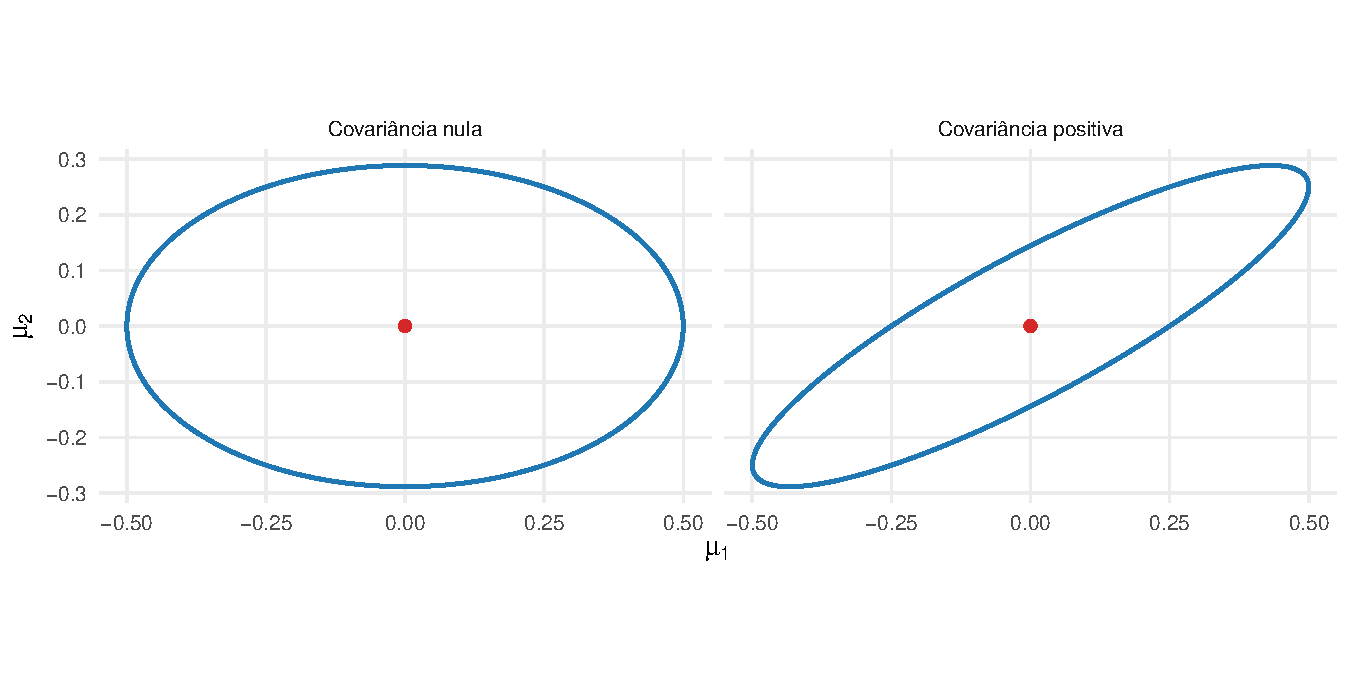
\includegraphics[width=1\linewidth,height=\textheight,keepaspectratio]{mod_2_inferencia_files/figure-pdf/fig-regioes-confianca-covariancias-1.pdf}

}

\caption{\label{fig-regioes-confianca-covariancias}Efeito da matriz de
covariâncias sobre a forma e a orientação da região de confiança para o
vetor de médias.}

\end{figure}%

Na primeira configuração da
Figura~\ref{fig-regioes-confianca-covariancias}, os eixos permanecem
alinhados às coordenadas originais. Na segunda, a covariância positiva
produz rotação do elipsoide. A região reflete, portanto, tanto as
variâncias marginais quanto a dependência entre as componentes.

\begin{tcolorbox}[enhanced jigsaw, colback=white, breakable, bottomrule=.15mm, left=2mm, arc=.35mm, rightrule=.15mm, colframe=quarto-callout-note-color-frame, toprule=.15mm, leftrule=.75mm, opacityback=0]

\vspace{-3mm}\textbf{Interpretação da cobertura}\vspace{3mm}

Antes da observação dos dados,

\[
\boldsymbol{\mathcal C}_{1-\alpha}
\]

é uma região aleatória que contém o verdadeiro vetor
\(\boldsymbol{\mu}\) com probabilidade \(1-\alpha\).

Depois da observação, a região está fixada. Na interpretação
frequentista, o parâmetro não passa a ser aleatório; a cobertura
refere-se ao comportamento do procedimento em repetições amostrais.

\end{tcolorbox}

\subsection{Intervalos simultâneos}\label{intervalos-simultuxe2neos}

Cada vetor

\[
\mathbf a
\in
\mathbb R^p
\]

define uma combinação linear \(\mathbf a^\top\boldsymbol{\mu}\). Como
todos esses funcionais são obtidos da mesma região elipsoidal, é
possível construir intervalos com cobertura simultânea para todas as
direções.

\begin{proposition}[Intervalos simultâneos de
Hotelling]\protect\hypertarget{prp-intervalos-simultaneos-hotelling}{}\label{prp-intervalos-simultaneos-hotelling}

Se

\[
\boldsymbol{\mathsf X}_1,
\ldots,
\boldsymbol{\mathsf X}_n
\stackrel{\mathrm{iid}}{\sim}
N_p
\left(
\boldsymbol{\mu},
\boldsymbol{\Sigma}
\right),
\qquad
\boldsymbol{\Sigma}
\succ
\mathbf0,
\]

com

\[
n>p
\qquad
\text{e}
\qquad
0<\alpha<1,
\]

e

\[
c_{\alpha,p,n}
=
\frac{
p(n-1)
}{
n-p
}
F_{p,n-p;1-\alpha},
\]

os intervalos

\begin{equation}\phantomsection\label{eq-intervalos-simultaneos-hotelling}{
\mathbf a^\top
\bar{\boldsymbol{\mathsf X}}
\pm
\sqrt{
\frac{
c_{\alpha,p,n}
}{
n
}
\mathbf a^\top
\boldsymbol{\mathsf S}
\mathbf a
},
\qquad
\mathbf a
\in
\mathbb R^p,
}\end{equation}

possuem cobertura simultânea \(1-\alpha\) para todas as combinações
lineares.

\end{proposition}

\begin{proof}
Se

\[
\boldsymbol{\mu}
\in
\boldsymbol{\mathcal C}_{1-\alpha},
\]

então

\[
\left(
\boldsymbol{\mu}
-
\bar{\boldsymbol{\mathsf X}}
\right)^\top
\boldsymbol{\mathsf S}^{-1}
\left(
\boldsymbol{\mu}
-
\bar{\boldsymbol{\mathsf X}}
\right)
\leq
\frac{
c_{\alpha,p,n}
}{
n
}.
\]

Pela desigualdade de Cauchy--Schwarz na geometria induzida por
\(\boldsymbol{\mathsf S}\),

\[
\left|
\mathbf a^\top
\left(
\boldsymbol{\mu}
-
\bar{\boldsymbol{\mathsf X}}
\right)
\right|
\leq
\sqrt{
\mathbf a^\top
\boldsymbol{\mathsf S}
\mathbf a
}
\sqrt{
\left(
\boldsymbol{\mu}
-
\bar{\boldsymbol{\mathsf X}}
\right)^\top
\boldsymbol{\mathsf S}^{-1}
\left(
\boldsymbol{\mu}
-
\bar{\boldsymbol{\mathsf X}}
\right)
}.
\]

Substituindo o limite da região, obtém-se
Equação~\ref{eq-intervalos-simultaneos-hotelling} simultaneamente para
todas as direções \(\mathbf a\).
\end{proof}

Após a observação dos dados,

\begin{equation}\phantomsection\label{eq-intervalo-simultaneo-hotelling-observado}{
\mathbf a^\top
\boldsymbol{\mu}
\in
\mathbf a^\top
\bar{\mathbf x}
\pm
\sqrt{
\frac{
c_{\alpha,p,n}
}{
n
}
\mathbf a^\top
\mathbf S
\mathbf a
}.
}\end{equation}

Para

\[
\mathbf a
=
\mathbf e_j,
\]

obtém-se o intervalo simultâneo para uma componente:

\begin{equation}\phantomsection\label{eq-intervalos-simultaneos-componentes-medias}{
\mu_j
\in
\bar{x}_j
\pm
\sqrt{
\frac{
c_{\alpha,p,n}
S_{jj}
}{
n
}
}.
}\end{equation}

Para

\[
\mathbf a
=
\mathbf e_j-\mathbf e_k,
\]

obtém-se

\begin{equation}\phantomsection\label{eq-intervalo-simultaneo-diferenca-componentes}{
\mu_j-\mu_k
\in
\bar{x}_j-\bar{x}_k
\pm
\sqrt{
\frac{
c_{\alpha,p,n}
}{
n
}
\left(
S_{jj}
+
S_{kk}
-
2S_{jk}
\right)
}.
}\end{equation}

Os intervalos de Hotelling fornecem cobertura simultânea para todas as
combinações lineares \(\mathbf a^\top\boldsymbol{\mu}\). Quando o
interesse está restrito a um conjunto finito e previamente especificado
de combinações, procedimentos como Bonferroni utilizam uma família de
inferências menor e podem produzir intervalos mais estreitos, dependendo
da estrutura de covariâncias e do número de comparações.

\subsection{Hipóteses lineares sobre o vetor de
médias}\label{hipuxf3teses-lineares-sobre-o-vetor-de-muxe9dias}

A hipótese

\[
H_0:
\boldsymbol{\mu}
=
\boldsymbol{\mu}_0
\]

especifica todo o vetor de médias. Em outros problemas, o interesse está
restrito a determinadas combinações lineares.

Considere

\[
\mathbf A
\in
\mathbb R^{h\times p},
\]

com

\[
\operatorname{posto}
\left(
\mathbf A
\right)
=
h
\leq
p,
\]

e

\[
\mathbf d
\in
\mathbb R^h.
\]

A hipótese é

\begin{equation}\phantomsection\label{eq-hipotese-linear-vetor-medias}{
H_0:
\mathbf A
\boldsymbol{\mu}
=
\mathbf d.
}\end{equation}

Cada linha de \(\mathbf A\) define uma restrição linear. A condição de
posto linha completo elimina restrições redundantes.

Defina

\[
\boldsymbol{\mathsf U}_i
=
\mathbf A
\boldsymbol{\mathsf X}_i.
\]

A distribuição decorre diretamente de
Proposição~\ref{prp-transformacao-afim-normal}.

Como \(\mathbf A\) possui posto linha completo e

\[
\boldsymbol{\Sigma}
\succ
\mathbf0,
\]

tem-se

\[
\mathbf A
\boldsymbol{\Sigma}
\mathbf A^\top
\succ
\mathbf0.
\]

A média e a covariância amostrais transformadas são

\[
\bar{\boldsymbol{\mathsf U}}
=
\mathbf A
\bar{\boldsymbol{\mathsf X}}
\]

e

\[
\boldsymbol{\mathsf S}_U
=
\mathbf A
\boldsymbol{\mathsf S}
\mathbf A^\top.
\]

Assim, o problema reduz-se exatamente à inferência sobre um vetor de
médias de dimensão \(h\).

\subsubsection{Covariância conhecida}\label{covariuxe2ncia-conhecida-1}

Quando \(\boldsymbol{\Sigma}\) é conhecida, defina

\begin{equation}\phantomsection\label{eq-estatistica-hipotese-linear-media-cov-conhecida}{
\mathsf Q_A
=
n
\left(
\mathbf A
\bar{\boldsymbol{\mathsf X}}
-
\mathbf d
\right)^\top
\left(
\mathbf A
\boldsymbol{\Sigma}
\mathbf A^\top
\right)^{-1}
\left(
\mathbf A
\bar{\boldsymbol{\mathsf X}}
-
\mathbf d
\right).
}\end{equation}

Sob \(H_0\),

\begin{equation}\phantomsection\label{eq-distribuicao-hipotese-linear-media-cov-conhecida}{
\mathsf Q_A
\sim
\chi_h^2.
}\end{equation}

Esse é
Proposição~\ref{prp-distribuicao-estatistica-media-covariancia-conhecida}
aplicado ao vetor transformado \(\boldsymbol{\mathsf U}_i\). Portanto,
os graus de liberdade são determinados pelas \(h\) combinações
linearmente independentes presentes na hipótese, e não pela dimensão
original \(p\).

\subsubsection{Covariância
desconhecida}\label{covariuxe2ncia-desconhecida}

Sob normalidade,

\[
\mathbf A
\boldsymbol{\mathsf S}
\mathbf A^\top
\succ
\mathbf0
\]

com probabilidade 1 quando

\begin{equation}\phantomsection\label{eq-condicao-t2-hipotese-linear-media}{
n>h.
}\end{equation}

\begin{proposition}[Distribuição para hipóteses lineares sobre a
média]\protect\hypertarget{prp-distribuicao-t2-hipotese-linear-media}{}\label{prp-distribuicao-t2-hipotese-linear-media}

Se

\[
\boldsymbol{\mathsf X}_1,
\ldots,
\boldsymbol{\mathsf X}_n
\stackrel{\mathrm{iid}}{\sim}
N_p
\left(
\boldsymbol{\mu},
\boldsymbol{\Sigma}
\right),
\qquad
\boldsymbol{\Sigma}
\succ
\mathbf0,
\]

e

\[
\mathbf A
\in
\mathbb R^{h\times p},
\qquad
1\leq h\leq p,
\qquad
\operatorname{posto}
\left(
\mathbf A
\right)
=
h,
\qquad
\mathbf d
\in
\mathbb R^h,
\qquad
n>h,
\]

então, sob

\[
H_0:
\mathbf A
\boldsymbol{\mu}
=
\mathbf d,
\]

a estatística

\begin{equation}\phantomsection\label{eq-t2-hipotese-linear-vetor-medias}{
\mathsf T_A^2
=
n
\left(
\mathbf A
\bar{\boldsymbol{\mathsf X}}
-
\mathbf d
\right)^\top
\left(
\mathbf A
\boldsymbol{\mathsf S}
\mathbf A^\top
\right)^{-1}
\left(
\mathbf A
\bar{\boldsymbol{\mathsf X}}
-
\mathbf d
\right)
}\end{equation}

satisfaz

\begin{equation}\phantomsection\label{eq-distribuicao-f-t2-hipotese-linear-media}{
\frac{
n-h
}{
h(n-1)
}
\mathsf T_A^2
\sim
F_{h,n-h}.
}\end{equation}

\end{proposition}

O resultado é Proposição~\ref{prp-distribuicao-t2-uma-amostra} aplicado
aos vetores transformados

\[
\boldsymbol{\mathsf U}_i
=
\mathbf A
\boldsymbol{\mathsf X}_i
\in
\mathbb R^h.
\]

Por isso, a condição dimensional passa de \(n>p\) para \(n>h\).

Assim, um teste de nível \(\alpha\) rejeita \(H_0\) quando

\begin{equation}\phantomsection\label{eq-regiao-critica-hipotese-linear-media}{
\mathsf T_{A,\mathrm{obs}}^2
>
\frac{
h(n-1)
}{
n-h
}
F_{h,n-h;1-\alpha},
}\end{equation}

em que

\begin{equation}\phantomsection\label{eq-t2-observado-hipotese-linear-media}{
\mathsf T_{A,\mathrm{obs}}^2
=
n
\left(
\mathbf A
\bar{\mathbf x}
-
\mathbf d
\right)^\top
\left(
\mathbf A
\mathbf S
\mathbf A^\top
\right)^{-1}
\left(
\mathbf A
\bar{\mathbf x}
-
\mathbf d
\right).
}\end{equation}

Uma consequência importante é que a condição dimensional depende de

\[
h,
\]

e não necessariamente de \(p\).

Assim, mesmo quando

\[
p\geq n
\]

e a matriz completa

\[
\boldsymbol{\mathsf S}
\]

é singular, uma hipótese de dimensão reduzida ainda pode admitir a
inferência clássica se

\[
n>h
\]

e

\[
\mathbf A
\boldsymbol{\mathsf S}
\mathbf A^\top
\]

for não singular.

Quando

\[
h=1,
\]

com

\[
\mathbf A
=
\mathbf a^\top,
\]

a hipótese

\[
H_0:
\mathbf a^\top
\boldsymbol{\mu}
=
d
\]

reduz-se ao teste \(t\) univariado aplicado à combinação linear

\[
\mathbf a^\top
\boldsymbol{\mathsf X}.
\]

Quando

\[
h=p,
\qquad
\mathbf A
=
\mathbf I_p,
\qquad
\mathbf d
=
\boldsymbol{\mu}_0,
\]

recupera-se o teste \(T^2\) para o vetor completo de médias.

\subsection{Relação com o modelo linear
multivariado}\label{relauxe7uxe3o-com-o-modelo-linear-multivariado}

O modelo de uma única população pode ser escrito como

\[
\boldsymbol{\mathcal Y}
=
\mathbf1_n
\boldsymbol{\mu}^\top
+
\boldsymbol{\mathcal E}.
\]

Nesse caso,

\[
\mathbf Z
=
\mathbf1_n
\]

e

\[
\mathbf B
=
\boldsymbol{\mu}^\top.
\]

Na hipótese geral de
Definição~\ref{def-hipotese-linear-geral-multivariada},

\[
H_0:
\mathbf C_1
\mathbf B
\mathbf C_2
=
\boldsymbol{\Theta}_0,
\]

tome

\[
\mathbf C_1
=
\begin{bmatrix}
1
\end{bmatrix},
\qquad
\mathbf C_2
=
\mathbf A^\top
\]

e

\[
\boldsymbol{\Theta}_0
=
\mathbf d^\top.
\]

Então,

\[
\mathbf C_1
\mathbf B
\mathbf C_2
=
\boldsymbol{\mu}^\top
\mathbf A^\top
=
\left(
\mathbf A
\boldsymbol{\mu}
\right)^\top.
\]

Portanto,

\[
H_0:
\mathbf A
\boldsymbol{\mu}
=
\mathbf d
\]

é um caso particular da hipótese linear geral do Capítulo 11.

Essa correspondência mostra que o teste \(T^2\) para uma média, as
hipóteses sobre combinações lineares e a inferência no modelo linear
multivariado utilizam a mesma estrutura. A próxima seção estende o
problema à comparação entre dois vetores de médias.

\section{Comparação entre dois vetores de
médias}\label{comparauxe7uxe3o-entre-dois-vetores-de-muxe9dias}

A comparação entre dois vetores de médias depende da relação entre as
unidades que produziram as observações. Duas estruturas serão
consideradas:

\begin{itemize}
\tightlist
\item
  \textbf{amostras independentes}, formadas por unidades distintas;
\item
  \textbf{observações pareadas}, nas quais cada unidade ou par fornece
  duas medições relacionadas.
\end{itemize}

Nos dois casos, o parâmetro de interesse é uma diferença entre vetores
de médias. O delineamento determina, porém, a matriz de covariâncias
dessa diferença e, consequentemente, a estatística utilizada na
inferência.

\subsection{Duas amostras
independentes}\label{duas-amostras-independentes}

Considere duas amostras mutuamente independentes:

\[
\boldsymbol{\mathsf X}_{11},
\ldots,
\boldsymbol{\mathsf X}_{1n_1}
\stackrel{\mathrm{iid}}{\sim}
N_p
\left(
\boldsymbol{\mu}_1,
\boldsymbol{\Sigma}
\right)
\]

e

\[
\boldsymbol{\mathsf X}_{21},
\ldots,
\boldsymbol{\mathsf X}_{2n_2}
\stackrel{\mathrm{iid}}{\sim}
N_p
\left(
\boldsymbol{\mu}_2,
\boldsymbol{\Sigma}
\right),
\]

com

\[
\boldsymbol{\Sigma}
\succ
\mathbf0.
\]

A especificação de uma mesma matriz

\[
\boldsymbol{\Sigma}
\]

para as duas populações é parte do modelo utilizado pelo procedimento
clássico com covariância agrupada.

O parâmetro de interesse é

\begin{equation}\phantomsection\label{eq-diferenca-vetores-medias-duas-amostras}{
\boldsymbol{\delta}
=
\boldsymbol{\mu}_1
-
\boldsymbol{\mu}_2
\in
\mathbb R^p.
}\end{equation}

Considere a hipótese

\begin{equation}\phantomsection\label{eq-hipotese-duas-amostras-independentes}{
H_0:
\boldsymbol{\mu}_1
-
\boldsymbol{\mu}_2
=
\boldsymbol{\delta}_0
}\end{equation}

contra

\[
H_1:
\boldsymbol{\mu}_1
-
\boldsymbol{\mu}_2
\neq
\boldsymbol{\delta}_0.
\]

A igualdade dos vetores de médias corresponde ao caso

\[
\boldsymbol{\delta}_0
=
\mathbf0.
\]

\subsubsection{Distribuição da diferença entre as
médias}\label{distribuiuxe7uxe3o-da-diferenuxe7a-entre-as-muxe9dias}

Aplicando Proposição~\ref{prp-distribuicao-media-amostral-normal}
separadamente às duas amostras,

\[
\bar{\boldsymbol{\mathsf X}}_1
\sim
N_p
\left(
\boldsymbol{\mu}_1,
\frac{
\boldsymbol{\Sigma}
}{
n_1
}
\right)
\]

e

\[
\bar{\boldsymbol{\mathsf X}}_2
\sim
N_p
\left(
\boldsymbol{\mu}_2,
\frac{
\boldsymbol{\Sigma}
}{
n_2
}
\right).
\]

Como as amostras são independentes,

\begin{equation}\phantomsection\label{eq-distribuicao-diferenca-medias-independentes}{
\bar{\boldsymbol{\mathsf X}}_1
-
\bar{\boldsymbol{\mathsf X}}_2
\sim
N_p
\left[
\boldsymbol{\mu}_1
-
\boldsymbol{\mu}_2,
\left(
\frac{1}{n_1}
+
\frac{1}{n_2}
\right)
\boldsymbol{\Sigma}
\right].
}\end{equation}

Para simplificar as expressões seguintes, defina o fator

\begin{equation}\phantomsection\label{eq-tamanho-efetivo-duas-amostras}{
n_{\mathrm{ef}}
=
\left(
\frac{1}{n_1}
+
\frac{1}{n_2}
\right)^{-1}
=
\frac{
n_1n_2
}{
n_1+n_2
}.
}\end{equation}

Então,

\[
\operatorname{Cov}
\left(
\bar{\boldsymbol{\mathsf X}}_1
-
\bar{\boldsymbol{\mathsf X}}_2
\right)
=
\frac{
\boldsymbol{\Sigma}
}{
n_{\mathrm{ef}}
}.
\]

A notação \(n_{\mathrm{ef}}\) será utilizada apenas como fator de escala
da covariância da diferença entre as médias. Ela não representa o número
total de observações nem os graus de liberdade do procedimento.

\subsubsection{Covariância agrupada}\label{covariuxe2ncia-agrupada}

Como \(\boldsymbol{\Sigma}\) é desconhecida, as duas amostras fornecem
estimativas da mesma matriz de covariâncias populacional. Essas
estimativas são combinadas ponderando cada SQPC pelos respectivos graus
de liberdade:

\begin{equation}\phantomsection\label{eq-covariancia-agrupada-duas-amostras}{
\boldsymbol{\mathsf S}_p
=
\frac{
(n_1-1)
\boldsymbol{\mathsf S}_1
+
(n_2-1)
\boldsymbol{\mathsf S}_2
}{
n_1+n_2-2
}.
}\end{equation}

A matriz \(\boldsymbol{\mathsf S}_p\) é denominada \textbf{matriz de
covariâncias agrupada}.

Após a observação,

\begin{equation}\phantomsection\label{eq-covariancia-agrupada-observada}{
\mathbf S_p
=
\frac{
(n_1-1)
\mathbf S_1
+
(n_2-1)
\mathbf S_2
}{
n_1+n_2-2
}.
}\end{equation}

Por Teorema~\ref{thm-distribuicao-sscp-amostral-normal}, sob o modelo de
covariância comum,

\[
(n_h-1)
\boldsymbol{\mathsf S}_h
\sim
W_p
\left(
n_h-1,
\boldsymbol{\Sigma}
\right),
\qquad
h=1,2.
\]

Como as duas amostras são independentes, essas matrizes Wishart também
são independentes. Portanto, Proposição~\ref{prp-aditividade-wishart}
pode ser aplicada às duas SQPCs.

\begin{proposition}[Distribuição da covariância
agrupada]\protect\hypertarget{prp-distribuicao-covariancia-agrupada}{}\label{prp-distribuicao-covariancia-agrupada}

Se as duas amostras são independentes, cada amostra é formada por
observações i.i.d. normais multivariadas em \(\mathbb R^p\) e ambas
possuem matriz de covariâncias comum

\[
\boldsymbol{\Sigma}
\succ
\mathbf0,
\]

com

\[
n_1\geq2
\qquad
\text{e}
\qquad
n_2\geq2,
\]

então

\begin{equation}\phantomsection\label{eq-distribuicao-wishart-covariancia-agrupada}{
(n_1+n_2-2)
\boldsymbol{\mathsf S}_p
\sim
W_p
\left(
n_1+n_2-2,
\boldsymbol{\Sigma}
\right).
}\end{equation}

Além disso,

\begin{equation}\phantomsection\label{eq-independencia-diferenca-medias-covariancia-agrupada}{
\bar{\boldsymbol{\mathsf X}}_1
-
\bar{\boldsymbol{\mathsf X}}_2
\perp
\boldsymbol{\mathsf S}_p.
}\end{equation}

\end{proposition}

\begin{proof}
Pela aditividade da distribuição de Wishart,

\[
\begin{aligned}
&
(n_1-1)
\boldsymbol{\mathsf S}_1
+
(n_2-1)
\boldsymbol{\mathsf S}_2
\\
&\sim
W_p
\left(
n_1+n_2-2,
\boldsymbol{\Sigma}
\right).
\end{aligned}
\]

A matriz no lado esquerdo é

\[
(n_1+n_2-2)
\boldsymbol{\mathsf S}_p.
\]

Sob normalidade, em cada amostra a média é independente da respectiva
matriz de covariâncias. A independência entre as duas amostras implica
então a independência entre

\[
\bar{\boldsymbol{\mathsf X}}_1
-
\bar{\boldsymbol{\mathsf X}}_2
\]

e

\[
\boldsymbol{\mathsf S}_p.
\]
\end{proof}

A distribuição em
Equação~\ref{eq-distribuicao-wishart-covariancia-agrupada} fornece

\[
E
\left(
\boldsymbol{\mathsf S}_p
\right)
=
\boldsymbol{\Sigma}.
\]

Além disso, por Proposição~\ref{prp-posto-matriz-wishart},

\[
\operatorname{posto}
\left(
\boldsymbol{\mathsf S}_p
\right)
=
\min
\left(
p,
n_1+n_2-2
\right)
\]

com probabilidade 1. Portanto,

\[
\boldsymbol{\mathsf S}_p
\succ
\mathbf0
\]

com probabilidade 1 quando

\begin{equation}\phantomsection\label{eq-condicao-inversao-covariancia-agrupada}{
n_1+n_2-2
\geq
p.
}\end{equation}

\subsubsection{\texorpdfstring{Estatística \(T^2\) para duas
amostras}{Estatística T\^{}2 para duas amostras}}\label{estatuxedstica-t2-para-duas-amostras}

\begin{definition}[Estatística \(T^2\) para duas amostras
independentes]\protect\hypertarget{def-t2-duas-amostras-independentes}{}\label{def-t2-duas-amostras-independentes}

Para testar

\[
H_0:
\boldsymbol{\mu}_1
-
\boldsymbol{\mu}_2
=
\boldsymbol{\delta}_0,
\]

quando

\[
\boldsymbol{\mathsf S}_p
\succ
\mathbf0,
\]

define-se

\begin{equation}\phantomsection\label{eq-t2-duas-amostras-independentes}{
\begin{aligned}
\mathsf T_{\mathrm{ind}}^2
=
n_{\mathrm{ef}}
\Big(
&
\bar{\boldsymbol{\mathsf X}}_1
-
\bar{\boldsymbol{\mathsf X}}_2
-
\boldsymbol{\delta}_0
\Big)^\top
\boldsymbol{\mathsf S}_p^{-1}
\\
&
\Big(
\bar{\boldsymbol{\mathsf X}}_1
-
\bar{\boldsymbol{\mathsf X}}_2
-
\boldsymbol{\delta}_0
\Big),
\end{aligned}
}\end{equation}

em que

\[
n_{\mathrm{ef}}
=
\frac{
n_1n_2
}{
n_1+n_2
}
\]

e

\[
\boldsymbol{\mathsf S}_p
=
\frac{
(n_1-1)
\boldsymbol{\mathsf S}_1
+
(n_2-1)
\boldsymbol{\mathsf S}_2
}{
n_1+n_2-2
}.
\]

\end{definition}

A estatística possui a mesma forma quadrática do \(T^2\) de uma amostra.
O vetor de afastamento é agora

\[
\bar{\boldsymbol{\mathsf X}}_1
-
\bar{\boldsymbol{\mathsf X}}_2
-
\boldsymbol{\delta}_0,
\]

e sua variabilidade é estimada pela matriz de covariâncias agrupada.

\begin{proposition}[Distribuição exata de \(T^2\) para duas
amostras]\protect\hypertarget{prp-distribuicao-t2-duas-amostras}{}\label{prp-distribuicao-t2-duas-amostras}

Se as duas amostras são independentes e

\[
\boldsymbol{\mathsf X}_{1i}
\stackrel{\mathrm{iid}}{\sim}
N_p
\left(
\boldsymbol{\mu}_1,
\boldsymbol{\Sigma}
\right),
\qquad
i=1,\ldots,n_1,
\]

e

\[
\boldsymbol{\mathsf X}_{2i}
\stackrel{\mathrm{iid}}{\sim}
N_p
\left(
\boldsymbol{\mu}_2,
\boldsymbol{\Sigma}
\right),
\qquad
i=1,\ldots,n_2,
\]

com

\[
\boldsymbol{\Sigma}
\succ
\mathbf0,
\qquad
n_1\geq2,
\qquad
n_2\geq2,
\]

e

\[
n_1+n_2-2
\geq
p,
\]

então, sob

\[
H_0:
\boldsymbol{\mu}_1
-
\boldsymbol{\mu}_2
=
\boldsymbol{\delta}_0,
\]

tem-se

\begin{equation}\phantomsection\label{eq-distribuicao-f-t2-duas-amostras}{
\frac{
n_1+n_2-p-1
}{
p(n_1+n_2-2)
}
\mathsf T_{\mathrm{ind}}^2
\sim
F_{
p,\,
n_1+n_2-p-1
}.
}\end{equation}

\end{proposition}

\begin{proof}
Sob \(H_0\), o vetor

\[
\boldsymbol{\mathsf V}
=
\sqrt{
n_{\mathrm{ef}}
}
\left(
\bar{\boldsymbol{\mathsf X}}_1
-
\bar{\boldsymbol{\mathsf X}}_2
-
\boldsymbol{\delta}_0
\right)
\]

satisfaz

\[
\boldsymbol{\mathsf V}
\sim
N_p
\left(
\mathbf0,
\boldsymbol{\Sigma}
\right).
\]

Além disso,

\[
\boldsymbol{\mathsf W}
=
(n_1+n_2-2)
\boldsymbol{\mathsf S}_p
\]

satisfaz, por Proposição~\ref{prp-distribuicao-covariancia-agrupada},

\[
\boldsymbol{\mathsf W}
\sim
W_p
\left(
n_1+n_2-2,
\boldsymbol{\Sigma}
\right)
\]

e

\[
\boldsymbol{\mathsf V}
\perp
\boldsymbol{\mathsf W}.
\]

A mesma estrutura normal--Wishart utilizada em
Proposição~\ref{prp-distribuicao-t2-uma-amostra} fornece

\[
\frac{
n_1+n_2-p-1
}{
p(n_1+n_2-2)
}
\mathsf T_{\mathrm{ind}}^2
\sim
F_{
p,\,
n_1+n_2-p-1
}.
\]
\end{proof}

Para os dados observados,

\begin{equation}\phantomsection\label{eq-t2-observado-duas-amostras}{
\begin{aligned}
\mathsf T_{\mathrm{ind,obs}}^2
=
n_{\mathrm{ef}}
\Big(
&
\bar{\mathbf x}_1
-
\bar{\mathbf x}_2
-
\boldsymbol{\delta}_0
\Big)^\top
\mathbf S_p^{-1}
\\
&
\Big(
\bar{\mathbf x}_1
-
\bar{\mathbf x}_2
-
\boldsymbol{\delta}_0
\Big).
\end{aligned}
}\end{equation}

Um teste de nível \(\alpha\) rejeita \(H_0\) quando

\begin{equation}\phantomsection\label{eq-regiao-critica-t2-duas-amostras}{
\mathsf T_{\mathrm{ind,obs}}^2
>
\frac{
p(n_1+n_2-2)
}{
n_1+n_2-p-1
}
F_{
p,\,
n_1+n_2-p-1;\,
1-\alpha
}.
}\end{equation}

Defina

\begin{equation}\phantomsection\label{eq-constante-regiao-confianca-duas-amostras}{
c_{\alpha,p,n_1,n_2}
=
\frac{
p(n_1+n_2-2)
}{
n_1+n_2-p-1
}
F_{
p,\,
n_1+n_2-p-1;\,
1-\alpha
}.
}\end{equation}

A inversão do teste fornece uma região de confiança de nível
\(1-\alpha\) para

\[
\boldsymbol{\delta}
=
\boldsymbol{\mu}_1-\boldsymbol{\mu}_2:
\]

\begin{equation}\phantomsection\label{eq-regiao-confianca-diferenca-medias-duas-amostras}{
\begin{aligned}
\mathcal C_{\delta,1-\alpha}
=
\Bigg\{
\boldsymbol{\theta}
\in
\mathbb R^p:
&
n_{\mathrm{ef}}
\Big(
\bar{\boldsymbol{\mathsf X}}_1
-
\bar{\boldsymbol{\mathsf X}}_2
-
\boldsymbol{\theta}
\Big)^\top
\boldsymbol{\mathsf S}_p^{-1}
\\
&
\Big(
\bar{\boldsymbol{\mathsf X}}_1
-
\bar{\boldsymbol{\mathsf X}}_2
-
\boldsymbol{\theta}
\Big)
\leq
c_{\alpha,p,n_1,n_2}
\Bigg\}.
\end{aligned}
}\end{equation}

A região é um elipsoide centrado em

\[
\bar{\boldsymbol{\mathsf X}}_1
-
\bar{\boldsymbol{\mathsf X}}_2,
\]

com orientação determinada pela matriz de covariâncias agrupada.

Para qualquer

\[
\mathbf a
\in
\mathbb R^p,
\]

os intervalos derivados dessa região são

\begin{equation}\phantomsection\label{eq-intervalos-simultaneos-duas-amostras}{
\mathbf a^\top
\left(
\bar{\boldsymbol{\mathsf X}}_1
-
\bar{\boldsymbol{\mathsf X}}_2
\right)
\pm
\sqrt{
\frac{
c_{\alpha,p,n_1,n_2}
}{
n_{\mathrm{ef}}
}
\mathbf a^\top
\boldsymbol{\mathsf S}_p
\mathbf a
}.
}\end{equation}

Esses intervalos fornecem cobertura simultânea para todas as combinações
lineares de \(\boldsymbol{\delta}\).

Quando

\[
p=1,
\]

o procedimento reduz-se ao quadrado do teste \(t\) para duas amostras
independentes com variâncias populacionais iguais:

\begin{equation}\phantomsection\label{eq-relacao-t2-t-duas-amostras}{
\mathsf T_{\mathrm{ind}}^2
=
\mathsf t_{\mathrm{pooled}}^2.
}\end{equation}

\subsection{Covariâncias populacionais
distintas}\label{covariuxe2ncias-populacionais-distintas}

O procedimento anterior foi construído sob

\[
\boldsymbol{\Sigma}_1
=
\boldsymbol{\Sigma}_2.
\]

Se

\[
\boldsymbol{\Sigma}_1
\neq
\boldsymbol{\Sigma}_2,
\]

a diferença entre as médias continua tendo, sob normalidade,

\begin{equation}\phantomsection\label{eq-covariancia-diferenca-medias-heterogenea}{
\bar{\boldsymbol{\mathsf X}}_1
-
\bar{\boldsymbol{\mathsf X}}_2
\sim
N_p
\left(
\boldsymbol{\mu}_1-\boldsymbol{\mu}_2,
\frac{
\boldsymbol{\Sigma}_1
}{
n_1
}
+
\frac{
\boldsymbol{\Sigma}_2
}{
n_2
}
\right).
}\end{equation}

Entretanto, a matriz agrupada satisfaz

\[
E
\left(
\boldsymbol{\mathsf S}_p
\right)
=
\frac{
(n_1-1)
\boldsymbol{\Sigma}_1
+
(n_2-1)
\boldsymbol{\Sigma}_2
}{
n_1+n_2-2
},
\]

e não estima diretamente

\[
\frac{
\boldsymbol{\Sigma}_1
}{
n_1
}
+
\frac{
\boldsymbol{\Sigma}_2
}{
n_2
}.
\]

Consequentemente, a estrutura normal--Wishart utilizada em
Proposição~\ref{prp-distribuicao-t2-duas-amostras} deixa de ser válida
com a matriz agrupada, e a transformação para a distribuição \(F\) não é
mais exata.

\begin{tcolorbox}[enhanced jigsaw, colback=white, breakable, bottomrule=.15mm, left=2mm, arc=.35mm, rightrule=.15mm, colframe=quarto-callout-caution-color-frame, toprule=.15mm, leftrule=.75mm, opacityback=0]

\vspace{-3mm}\textbf{Papel da homogeneidade das covariâncias}\vspace{3mm}

A igualdade

\[
\boldsymbol{\Sigma}_1
=
\boldsymbol{\Sigma}_2
\]

não é necessária para o \(T^2\) de uma amostra nem para o procedimento
pareado.

Ela é uma hipótese específica do procedimento de duas amostras
independentes que utiliza a covariância agrupada.

Quando as covariâncias populacionais são distintas, o problema
inferencial é diferente e requer outro procedimento ou outra
aproximação. A simples substituição de \(\mathbf S_p\) por uma matriz
alternativa não preserva automaticamente a distribuição \(F\) clássica.

\end{tcolorbox}

\subsection{Observações pareadas}\label{observauxe7uxf5es-pareadas}

No delineamento pareado, considere

\[
\left(
\boldsymbol{\mathsf X}_i,
\boldsymbol{\mathsf Y}_i
\right),
\qquad
i=1,\ldots,n,
\]

em que os pares são independentes entre si, mas as duas medições dentro
de cada par podem ser dependentes.

O número

\[
n
\]

representa o número de pares completos.

Defina

\begin{equation}\phantomsection\label{eq-vetor-diferencas-pareadas}{
\boldsymbol{\mathsf D}_i
=
\boldsymbol{\mathsf X}_i
-
\boldsymbol{\mathsf Y}_i.
}\end{equation}

O vetor médio das diferenças é

\begin{equation}\phantomsection\label{eq-media-vetor-diferencas-pareadas}{
\boldsymbol{\delta}
=
E
\left(
\boldsymbol{\mathsf D}_i
\right)
=
\boldsymbol{\mu}_X
-
\boldsymbol{\mu}_Y.
}\end{equation}

Sua matriz de covariâncias é

\begin{equation}\phantomsection\label{eq-covariancia-vetor-diferencas-pareadas}{
\boldsymbol{\Sigma}_D
=
\boldsymbol{\Sigma}_X
+
\boldsymbol{\Sigma}_Y
-
\boldsymbol{\Sigma}_{XY}
-
\boldsymbol{\Sigma}_{YX}.
}\end{equation}

A expressão mostra por que a associação dentro dos pares deve ser
preservada: ela participa diretamente da variabilidade das diferenças.

A hipótese é

\begin{equation}\phantomsection\label{eq-hipotese-observacoes-pareadas}{
H_0:
\boldsymbol{\delta}
=
\boldsymbol{\delta}_0.
}\end{equation}

Para comparar diretamente as duas condições,

\[
\boldsymbol{\delta}_0
=
\mathbf0.
\]

Depois de formar as diferenças, cada par produz um único vetor

\[
\boldsymbol{\mathsf D}_i.
\]

A comparação entre as duas condições passa, portanto, a ser uma
inferência sobre o vetor médio de uma única população de diferenças:

\[
\boldsymbol{\mathsf D}_1,
\ldots,
\boldsymbol{\mathsf D}_n.
\]

Suponha

\[
\boldsymbol{\mathsf D}_1,
\ldots,
\boldsymbol{\mathsf D}_n
\stackrel{\mathrm{iid}}{\sim}
N_p
\left(
\boldsymbol{\delta},
\boldsymbol{\Sigma}_D
\right),
\]

com

\[
\boldsymbol{\Sigma}_D
\succ
\mathbf0.
\]

A média amostral das diferenças é

\begin{equation}\phantomsection\label{eq-media-amostral-diferencas-pareadas}{
\bar{\boldsymbol{\mathsf D}}
=
\frac1n
\sum_{i=1}^{n}
\boldsymbol{\mathsf D}_i
=
\bar{\boldsymbol{\mathsf X}}
-
\bar{\boldsymbol{\mathsf Y}}.
}\end{equation}

A matriz de covariâncias amostral é

\begin{equation}\phantomsection\label{eq-covariancia-amostral-diferencas-pareadas}{
\boldsymbol{\mathsf S}_D
=
\frac{1}{n-1}
\sum_{i=1}^{n}
\left(
\boldsymbol{\mathsf D}_i
-
\bar{\boldsymbol{\mathsf D}}
\right)
\left(
\boldsymbol{\mathsf D}_i
-
\bar{\boldsymbol{\mathsf D}}
\right)^\top.
}\end{equation}

Quando as matrizes são calculadas sobre os mesmos pares completos,

\begin{equation}\phantomsection\label{eq-decomposicao-covariancia-amostral-diferencas}{
\boldsymbol{\mathsf S}_D
=
\boldsymbol{\mathsf S}_X
+
\boldsymbol{\mathsf S}_Y
-
\boldsymbol{\mathsf S}_{XY}
-
\boldsymbol{\mathsf S}_{YX}.
}\end{equation}

A decomposição populacional em
Equação~\ref{eq-covariancia-vetor-diferencas-pareadas} utiliza a
covariância cruzada definida em Definição~\ref{def-covariancia-cruzada}.
Sua contraparte amostral em
Equação~\ref{eq-decomposicao-covariancia-amostral-diferencas} utiliza a
matriz definida em Definição~\ref{def-covariancia-cruzada-amostral}.

\begin{definition}[Estatística \(T^2\) para observações
pareadas]\protect\hypertarget{def-t2-observacoes-pareadas}{}\label{def-t2-observacoes-pareadas}

Para os vetores de diferenças pareadas

\[
\boldsymbol{\mathsf D}_i
=
\boldsymbol{\mathsf X}_i
-
\boldsymbol{\mathsf Y}_i,
\qquad
i=1,\ldots,n,
\]

com vetor de médias amostrais \(\bar{\boldsymbol{\mathsf D}}\) e matriz
de covariâncias amostral \(\boldsymbol{\mathsf S}_D\succ\mathbf0\),
define-se

\begin{equation}\phantomsection\label{eq-t2-observacoes-pareadas}{
\mathsf T_{\mathrm{par}}^2
=
n
\left(
\bar{\boldsymbol{\mathsf D}}
-
\boldsymbol{\delta}_0
\right)^\top
\boldsymbol{\mathsf S}_D^{-1}
\left(
\bar{\boldsymbol{\mathsf D}}
-
\boldsymbol{\delta}_0
\right).
}\end{equation}

\end{definition}

\begin{proposition}[Distribuição exata de \(T^2\) para observações
pareadas]\protect\hypertarget{prp-distribuicao-t2-observacoes-pareadas}{}\label{prp-distribuicao-t2-observacoes-pareadas}

Se

\[
\boldsymbol{\mathsf D}_1,
\ldots,
\boldsymbol{\mathsf D}_n
\stackrel{\mathrm{iid}}{\sim}
N_p
\left(
\boldsymbol{\delta},
\boldsymbol{\Sigma}_D
\right),
\]

com

\[
\boldsymbol{\Sigma}_D
\succ
\mathbf0
\]

e

\[
n>p,
\]

então, sob

\[
H_0:
\boldsymbol{\delta}
=
\boldsymbol{\delta}_0,
\]

tem-se

\begin{equation}\phantomsection\label{eq-distribuicao-f-t2-pareado}{
\frac{
n-p
}{
p(n-1)
}
\mathsf T_{\mathrm{par}}^2
\sim
F_{p,n-p}.
}\end{equation}

\end{proposition}

A proposição é Proposição~\ref{prp-distribuicao-t2-uma-amostra} aplicada
à amostra

\[
\boldsymbol{\mathsf D}_1,
\ldots,
\boldsymbol{\mathsf D}_n.
\]

Por isso, o número de observações utilizado no teste é o número de pares
completos.

Para os dados observados,

\begin{equation}\phantomsection\label{eq-t2-observado-pareado}{
\mathsf T_{\mathrm{par,obs}}^2
=
n
\left(
\bar{\mathbf d}
-
\boldsymbol{\delta}_0
\right)^\top
\mathbf S_D^{-1}
\left(
\bar{\mathbf d}
-
\boldsymbol{\delta}_0
\right).
}\end{equation}

Um teste de nível \(\alpha\) rejeita \(H_0\) quando

\begin{equation}\phantomsection\label{eq-regiao-critica-t2-pareado}{
\mathsf T_{\mathrm{par,obs}}^2
>
\frac{
p(n-1)
}{
n-p
}
F_{p,n-p;1-\alpha}.
}\end{equation}

Quando

\[
p=1,
\]

recupera-se o quadrado do teste \(t\) pareado:

\begin{equation}\phantomsection\label{eq-relacao-t2-t-pareado}{
\mathsf T_{\mathrm{par}}^2
=
\mathsf t_{\mathrm{par}}^2.
}\end{equation}

Aplicando Proposição~\ref{prp-regiao-confianca-vetor-medias} à população
de diferenças, obtém-se a região de confiança de nível \(1-\alpha\)

\begin{equation}\phantomsection\label{eq-regiao-confianca-media-diferencas}{
\begin{aligned}
\mathcal C_{D,1-\alpha}
=
\Bigg\{
\boldsymbol{\theta}
\in
\mathbb R^p:
&
n
\left(
\bar{\boldsymbol{\mathsf D}}
-
\boldsymbol{\theta}
\right)^\top
\boldsymbol{\mathsf S}_D^{-1}
\\
&
\left(
\bar{\boldsymbol{\mathsf D}}
-
\boldsymbol{\theta}
\right)
\leq
c_{\alpha,p,n}
\Bigg\},
\end{aligned}
}\end{equation}

em que \(c_{\alpha,p,n}\) foi definida em
Equação~\ref{eq-constante-regiao-confianca-hotelling}.

Para qualquer

\[
\mathbf a
\in
\mathbb R^p,
\]

Proposição~\ref{prp-intervalos-simultaneos-hotelling} fornece

\begin{equation}\phantomsection\label{eq-intervalos-simultaneos-diferencas-pareadas}{
\mathbf a^\top
\bar{\boldsymbol{\mathsf D}}
\pm
\sqrt{
\frac{
c_{\alpha,p,n}
}{
n
}
\mathbf a^\top
\boldsymbol{\mathsf S}_D
\mathbf a
}.
}\end{equation}

Assim, teste, região de confiança e intervalos simultâneos do caso
pareado são os resultados de uma amostra aplicados aos vetores de
diferenças.

\begin{tcolorbox}[enhanced jigsaw, colback=white, breakable, bottomrule=.15mm, left=2mm, arc=.35mm, rightrule=.15mm, colframe=quarto-callout-caution-color-frame, toprule=.15mm, leftrule=.75mm, opacityback=0]

\vspace{-3mm}\textbf{Preservação do pareamento}\vspace{3mm}

O procedimento deve ser aplicado às diferenças construídas com a
correspondência correta entre as unidades.

Tratar as duas condições como amostras independentes elimina da análise
a covariância intrapar e utiliza uma estrutura de variabilidade
diferente daquela determinada pelo delineamento.

A normalidade necessária ao resultado exato refere-se à distribuição dos
vetores

\[
\boldsymbol{\mathsf D}_i,
\]

e não exige, separadamente, que cada uma das duas condições possua
distribuição marginal normal multivariada.

\end{tcolorbox}

A Tabela Tabela~\ref{tbl-comparacao-independentes-pareadas} resume a
diferença entre os dois delineamentos.

\begin{longtable}[]{@{}
  >{\raggedright\arraybackslash}p{(\linewidth - 4\tabcolsep) * \real{0.3333}}
  >{\raggedright\arraybackslash}p{(\linewidth - 4\tabcolsep) * \real{0.3333}}
  >{\raggedright\arraybackslash}p{(\linewidth - 4\tabcolsep) * \real{0.3333}}@{}}
\caption{Comparação entre o \(T^2\) para amostras independentes e para
observações
pareadas.}\label{tbl-comparacao-independentes-pareadas}\tabularnewline
\toprule\noalign{}
\begin{minipage}[b]{\linewidth}\raggedright
Característica
\end{minipage} & \begin{minipage}[b]{\linewidth}\raggedright
Amostras independentes
\end{minipage} & \begin{minipage}[b]{\linewidth}\raggedright
Observações pareadas
\end{minipage} \\
\midrule\noalign{}
\endfirsthead
\toprule\noalign{}
\begin{minipage}[b]{\linewidth}\raggedright
Característica
\end{minipage} & \begin{minipage}[b]{\linewidth}\raggedright
Amostras independentes
\end{minipage} & \begin{minipage}[b]{\linewidth}\raggedright
Observações pareadas
\end{minipage} \\
\midrule\noalign{}
\endhead
\bottomrule\noalign{}
\endlastfoot
unidade básica & observações distintas & par de medições relacionadas \\
parâmetro & \(\boldsymbol{\mu}_1-\boldsymbol{\mu}_2\) &
\(E(\boldsymbol{\mathsf D})\) \\
matriz usada na forma quadrática & covariância comum estimada por
\(\boldsymbol{\mathsf S}_p\) & covariância das diferenças estimada por
\(\boldsymbol{\mathsf S}_D\) \\
dependência entre as duas medições & não há correspondência entre
unidades das duas amostras & incorporada em \(\boldsymbol{\Sigma}_{XY}\)
e \(\boldsymbol{\Sigma}_{YX}\) e, portanto, em
\(\boldsymbol{\Sigma}_D\) \\
graus de liberdade da matriz de covariâncias & \(n_1+n_2-2\) &
\(n-1\) \\
condição clássica de inversão & \(n_1+n_2-2\geq p\) & \(n>p\) \\
redução univariada & teste \(t\) com variâncias iguais & teste \(t\)
pareado \\
\end{longtable}

Os dois procedimentos utilizam a mesma lógica inferencial, mas estimam
estruturas de variabilidade distintas. Essa diferença será retomada na
seção seguinte ao organizar as condições necessárias à inferência
multivariada clássica.

\section{Condições e limites da inferência
clássica}\label{condiuxe7uxf5es-e-limites-da-inferuxeancia-cluxe1ssica}

Os resultados desenvolvidos neste capítulo dependem da estrutura
probabilística da amostra, das hipóteses específicas de cada
procedimento e do posto das matrizes envolvidas. Essas condições não são
intercambiáveis: uma hipótese necessária para um procedimento pode ser
irrelevante para outro.

Quatro aspectos organizam a validade da inferência clássica:

\begin{enumerate}
\def\labelenumi{\arabic{enumi}.}
\tightlist
\item
  independência entre as unidades amostrais na estrutura especificada
  pelo delineamento;
\item
  normalidade multivariada quando se utilizam distribuições exatas
  normal--Wishart;
\item
  covariância comum nos procedimentos que a pressupõem;
\item
  posto suficiente das matrizes utilizadas nas formas quadráticas,
  inversas e determinantes.
\end{enumerate}

\subsection{Independência, normalidade e covariância
comum}\label{independuxeancia-normalidade-e-covariuxe2ncia-comum}

\subsubsection{Independência}\label{independuxeancia}

Nos resultados para uma amostra,

\[
\boldsymbol{\mathsf X}_1,
\ldots,
\boldsymbol{\mathsf X}_n
\]

são consideradas independentes.

Para duas amostras independentes, exige-se também independência entre as
duas amostras. No delineamento pareado, admite-se dependência entre as
duas medições de um mesmo par, mas os pares devem ser independentes
entre si.

No modelo linear multivariado clássico,

\[
\operatorname{Cov}
\left[
\operatorname{vec}
\left(
\boldsymbol{\mathcal E}
\right)
\mid
\mathbf Z
\right]
=
\boldsymbol{\Sigma}
\otimes
\mathbf I_n
\]

expressa a ausência de covariância residual entre unidades distintas.

A independência é determinada principalmente pelo processo de amostragem
e pelo delineamento do estudo. Se existe dependência entre unidades e
ela não é incorporada ao modelo, expressões como

\[
\operatorname{Cov}
\left(
\bar{\boldsymbol{\mathsf X}}
\right)
=
\frac{
\boldsymbol{\Sigma}
}{
n
}
\]

podem deixar de representar a variabilidade efetiva da média amostral.

Consequentemente, estatísticas construídas com essa estrutura podem
apresentar níveis de significância e coberturas diferentes dos valores
nominais.

\begin{tcolorbox}[enhanced jigsaw, colback=white, breakable, bottomrule=.15mm, left=2mm, arc=.35mm, rightrule=.15mm, colframe=quarto-callout-note-color-frame, toprule=.15mm, leftrule=.75mm, opacityback=0]

\vspace{-3mm}\textbf{Independência e delineamento}\vspace{3mm}

A independência não é estabelecida por um teste aplicado aos valores
observados. Ela deve ser avaliada a partir da forma como as unidades
foram selecionadas, agrupadas e mensuradas.

Dependência espacial, temporal, hierárquica ou decorrente de medidas
repetidas exige uma estrutura probabilística compatível com o
delineamento.

\end{tcolorbox}

\subsubsection{Normalidade multivariada}\label{normalidade-multivariada}

A normalidade multivariada sustenta os principais resultados exatos
deste capítulo. Sob esse modelo foram estabelecidas:

\begin{itemize}
\tightlist
\item
  a distribuição normal da média em
  Proposição~\ref{prp-distribuicao-media-amostral-normal};
\item
  a distribuição Wishart da SQPC amostral em
  Teorema~\ref{thm-distribuicao-sscp-amostral-normal};
\item
  a independência entre média e covariância amostrais em
  Teorema~\ref{thm-independencia-media-covariancia-normal};
\item
  a distribuição \(F\) exata do \(T^2\) em
  Proposição~\ref{prp-distribuicao-t2-uma-amostra};
\item
  as distribuições Wishart e as independências associadas ao modelo
  linear multivariado em
  Proposição~\ref{prp-distribuicao-sscp-hipotese-nula}.
\end{itemize}

Esses resultados devem ser distinguidos das propriedades que dependem
apenas de momentos. Por exemplo,
Proposição~\ref{prp-media-amostral-momentos} e
Proposição~\ref{prp-nao-viesamento-covariancia-amostral} não exigem
normalidade.

Fora do modelo normal, a distribuição Wishart e as independências
utilizadas para construir as distribuições exatas deixam, em geral, de
estar disponíveis. No regime de dimensão fixa de
Equação~\ref{eq-regime-assintotico-classico}, resultados assintóticos
podem ainda ser obtidos.

Se as observações são i.i.d., possuem matriz de covariâncias finita e
positiva definida, e as condições de Teorema~\ref{thm-tcl-multivariado}
e Proposição~\ref{prp-consistencia-covariancia-amostral} são
satisfeitas, então, sob

\[
H_0:
\boldsymbol{\mu}
=
\boldsymbol{\mu}_0,
\]

o Teorema Central do Limite multivariado e o teorema de Slutsky fornecem

\begin{equation}\phantomsection\label{eq-t2-assintotico-sem-normalidade}{
\mathsf T^2
\xrightarrow{d}
\chi_p^2.
}\end{equation}

Essa convergência não implica que

\[
\frac{
n-p
}{
p(n-1)
}
\mathsf T^2
\sim
F_{p,n-p}
\]

seja uma distribuição exata em amostras finitas fora do modelo normal.

\begin{tcolorbox}[enhanced jigsaw, colback=white, breakable, bottomrule=.15mm, left=2mm, arc=.35mm, rightrule=.15mm, colframe=quarto-callout-caution-color-frame, toprule=.15mm, leftrule=.75mm, opacityback=0]

\vspace{-3mm}\textbf{Exato e assintótico}\vspace{3mm}

A normalidade não é necessária para definir médias, covariâncias,
matrizes SQPC ou formas quadráticas.

Neste capítulo, ela é utilizada para obter determinadas distribuições
amostrais \textbf{exatas}. Fora desse modelo, uma aproximação
assintótica depende das condições do resultado limite utilizado e do
regime em que \(n\) e \(p\) variam.

\end{tcolorbox}

\subsubsection{Covariância comum}\label{covariuxe2ncia-comum}

A hipótese

\[
\boldsymbol{\Sigma}_1
=
\boldsymbol{\Sigma}_2
\]

não pertence a todos os procedimentos multivariados.

Ela foi utilizada especificamente no teste de duas amostras
independentes com covariância agrupada, pois permite obter

\[
(n_1+n_2-2)
\boldsymbol{\mathsf S}_p
\sim
W_p
\left(
n_1+n_2-2,
\boldsymbol{\Sigma}
\right).
\]

Quando

\[
\boldsymbol{\Sigma}_1
\neq
\boldsymbol{\Sigma}_2,
\]

a covariância da diferença entre as médias é a apresentada em
Equação~\ref{eq-covariancia-diferenca-medias-heterogenea},

\[
\frac{
\boldsymbol{\Sigma}_1
}{
n_1
}
+
\frac{
\boldsymbol{\Sigma}_2
}{
n_2
},
\]

e a matriz agrupada não conduz à distribuição \(F\) exata da
Proposição~\ref{prp-distribuicao-t2-duas-amostras}.

No procedimento pareado, essa hipótese não é necessária. A matriz
relevante é

\[
\boldsymbol{\Sigma}_D
=
\operatorname{Cov}
\left(
\boldsymbol{\mathsf X}_i
-
\boldsymbol{\mathsf Y}_i
\right).
\]

No modelo linear multivariado clássico, a estrutura

\[
\operatorname{Cov}
\left(
\boldsymbol{\varepsilon}_i
\mid
\mathbf Z
\right)
=
\boldsymbol{\Sigma}
\]

supõe uma matriz residual comum às unidades representadas pelo modelo.

Assim, a homogeneidade deve ser entendida como uma hipótese do
\textbf{procedimento que utiliza uma matriz de covariâncias comum}, e
não como uma condição universal da inferência multivariada.

\subsection{Posto, dimensão e tamanho
amostral}\label{posto-dimensuxe3o-e-tamanho-amostral}

As formas clássicas das estatísticas utilizam matrizes inversas. A
condição necessária depende da dimensão efetivamente utilizada em cada
problema.

\subsubsection{Uma amostra}\label{uma-amostra}

Sob normalidade não singular,

\[
\operatorname{posto}
\left(
\boldsymbol{\mathsf S}
\right)
=
\min
\left(
p,n-1
\right)
\]

com probabilidade 1.

Portanto,

\[
\boldsymbol{\mathsf S}^{-1}
\]

existe com probabilidade 1 se, e somente se,

\[
n>p.
\]

Essa é também a condição que torna positivo o segundo grau de liberdade

\[
n-p
\]

da distribuição

\[
F_{p,n-p}.
\]

\subsubsection{Hipóteses de dimensão
reduzida}\label{hipuxf3teses-de-dimensuxe3o-reduzida}

Para

\[
H_0:
\mathbf A
\boldsymbol{\mu}
=
\mathbf d,
\]

com

\[
\operatorname{posto}
\left(
\mathbf A
\right)
=
h,
\]

a matriz relevante é

\[
\mathbf A
\boldsymbol{\mathsf S}
\mathbf A^\top.
\]

A condição clássica passa a ser

\[
n>h.
\]

Portanto, a singularidade da matriz completa \(\boldsymbol{\mathsf S}\)
não impede necessariamente a inferência sobre combinações previamente
especificadas de dimensão menor.

\subsubsection{Duas amostras
independentes}\label{duas-amostras-independentes-1}

Sob normalidade e covariância comum,

\[
\operatorname{posto}
\left(
\boldsymbol{\mathsf S}_p
\right)
=
\min
\left(
p,
n_1+n_2-2
\right)
\]

com probabilidade 1.

A inversão clássica requer

\[
n_1+n_2-2
\geq
p.
\]

Sob essa condição,

\[
n_1+n_2-p-1
>
0,
\]

como necessário para a distribuição \(F\) da
Proposição~\ref{prp-distribuicao-t2-duas-amostras}.

\subsubsection{Modelo linear
multivariado}\label{modelo-linear-multivariado-1}

Se

\[
r
=
\operatorname{posto}
\left(
\mathbf Z
\right),
\]

então

\[
\boldsymbol{\mathsf E}_{\mathrm{res}}
\mid
\mathbf Z
\sim
W_p
\left(
n-r,
\boldsymbol{\Sigma}
\right),
\]

e

\[
\operatorname{posto}
\left(
\boldsymbol{\mathsf E}_{\mathrm{res}}
\right)
=
\min
\left(
p,n-r
\right)
\]

com probabilidade 1.

Logo,

\[
\boldsymbol{\mathsf E}_{\mathrm{res}}
\succ
\mathbf0
\]

com probabilidade 1 quando

\[
n-r
\geq
p.
\]

Para combinações de respostas definidas por

\[
\mathbf C_2
\in
\mathbb R^{p\times s},
\]

com posto coluna completo,

\[
\boldsymbol{\mathsf E}_{C_2}
=
\mathbf C_2^\top
\boldsymbol{\mathsf E}_{\mathrm{res}}
\mathbf C_2
\]

é positiva definida com probabilidade 1 quando

\[
n-r
\geq
s,
\]

conforme Equação~\ref{eq-condicao-inversibilidade-erro-transformado}.

Portanto, a condição de posto depende da dimensão do objeto que
efetivamente participa da inferência. Uma matriz de covariâncias
completa pode ser singular e, ainda assim, determinadas combinações
previamente especificadas admitirem inferência clássica em um espaço de
menor dimensão.

\begin{tcolorbox}[enhanced jigsaw, colback=white, breakable, bottomrule=.15mm, left=2mm, arc=.35mm, rightrule=.15mm, colframe=quarto-callout-note-color-frame, toprule=.15mm, leftrule=.75mm, opacityback=0]

\vspace{-3mm}\textbf{Existência e estabilidade}\vspace{3mm}

A existência de uma inversa é uma condição algébrica; sua estabilidade
depende também da separação entre os autovalores da matriz.

O efeito do condicionamento sobre a inversão de matrizes de covariâncias
foi discutido em Equação~\ref{eq-numero-condicao-covariancia}. Assim,
uma matriz pode possuir posto completo e ainda produzir formas
quadráticas sensíveis a pequenas perturbações dos dados.

\end{tcolorbox}

A Tabela Tabela~\ref{tbl-condicoes-inferencia-classica} resume as
condições centrais dos procedimentos desenvolvidos neste capítulo.

\begin{longtable}[]{@{}
  >{\raggedright\arraybackslash}p{(\linewidth - 4\tabcolsep) * \real{0.3333}}
  >{\raggedright\arraybackslash}p{(\linewidth - 4\tabcolsep) * \real{0.3333}}
  >{\raggedright\arraybackslash}p{(\linewidth - 4\tabcolsep) * \real{0.3333}}@{}}
\caption{Condições centrais para os resultados exatos da inferência
multivariada
clássica.}\label{tbl-condicoes-inferencia-classica}\tabularnewline
\toprule\noalign{}
\begin{minipage}[b]{\linewidth}\raggedright
Procedimento
\end{minipage} & \begin{minipage}[b]{\linewidth}\raggedright
Estrutura probabilística para o resultado exato
\end{minipage} & \begin{minipage}[b]{\linewidth}\raggedright
Condição principal de posto
\end{minipage} \\
\midrule\noalign{}
\endfirsthead
\toprule\noalign{}
\begin{minipage}[b]{\linewidth}\raggedright
Procedimento
\end{minipage} & \begin{minipage}[b]{\linewidth}\raggedright
Estrutura probabilística para o resultado exato
\end{minipage} & \begin{minipage}[b]{\linewidth}\raggedright
Condição principal de posto
\end{minipage} \\
\midrule\noalign{}
\endhead
\bottomrule\noalign{}
\endlastfoot
média com \(\boldsymbol{\Sigma}\) conhecida & normalidade da média
amostral & \(\boldsymbol{\Sigma}\succ\mathbf0\) \\
\(T^2\) de uma amostra & amostra normal multivariada & \(n>p\) \\
\(T^2\) para \(\mathbf A\boldsymbol{\mu}=\mathbf d\) & amostra normal
multivariada & \(n>h\) \\
duas amostras independentes & normalidade, independência e covariância
comum & \(n_1+n_2-2\geq p\) \\
observações pareadas & normalidade dos vetores de diferenças &
\(n>p\) \\
modelo linear multivariado & normalidade matricial dos erros &
\(n-r\geq p\) para \(\mathbf E\succ\mathbf0\) \\
combinações de \(s\) respostas & normalidade matricial dos erros &
\(n-r\geq s\) para \(\mathbf E_{C_2}\succ\mathbf0\) \\
\end{longtable}

\subsection{Aprofundamento: alta dimensão e
robustez}\label{aprofundamento-alta-dimensuxe3o-e-robustez}

A teoria desenvolvida neste capítulo é predominantemente uma teoria de
\textbf{dimensão fixa}, na qual a informação amostral cresce enquanto a
dimensão permanece constante. Quando a dimensão é grande em relação ao
tamanho amostral, singularidade e instabilidade tornam-se parte central
do problema.

\subsubsection{Alta dimensão}\label{alta-dimensuxe3o}

Os limites de posto estabelecidos neste capítulo mostram que a
inferência clássica baseada em inversas deixa de estar disponível quando
a dimensão ultrapassa os graus de liberdade correspondentes. Para uma
amostra, por exemplo, Equação~\ref{eq-posto-sscp-amostral} implica que

\[
p\geq n
\]

torna \(\boldsymbol{\mathsf S}\) necessariamente singular. Situações
análogas ocorrem para a covariância agrupada quando

\[
p>n_1+n_2-2
\]

e para a SQPC residual do modelo linear quando

\[
p>n-r.
\]

O Capítulo 10 distinguiu duas respostas algébricas a problemas dessa
natureza: a pseudoinversa em
Equação~\ref{eq-pseudoinversa-covariancia-amostral} e a regularização da
matriz de covariâncias em
Definição~\ref{def-estimador-contracao-covariancia}. Nenhuma dessas
substituições preserva automaticamente as distribuições inferenciais
derivadas neste capítulo para a inversa clássica.

Por exemplo, substituir \(\boldsymbol{\mathsf S}^{-1}\) por
\(\boldsymbol{\mathsf S}^{+}\) modifica a estatística \(T^2\) e não
permite utilizar automaticamente

\[
\frac{
n-p
}{
p(n-1)
}
\mathsf T^2
\sim
F_{p,n-p}.
\]

O mesmo ocorre quando \(\boldsymbol{\mathsf S}\) é substituída por um
estimador regularizado.

Uma alternativa diferente consiste em formular previamente a hipótese em
um espaço de menor dimensão. Isso ocorre em

\[
H_0:
\mathbf A
\boldsymbol{\mu}
=
\mathbf d
\]

e, no modelo linear, em

\[
H_0:
\mathbf C_1
\mathbf B
\mathbf C_2
=
\boldsymbol{\Theta}_0.
\]

Nesse caso, a condição de posto depende da dimensão das combinações
efetivamente examinadas. Se essas combinações forem escolhidas a partir
dos próprios dados, entretanto, o processo de seleção também integra o
procedimento inferencial.

Testes específicos para alta dimensão, regularização inferencial,
reamostragem e procedimentos baseados em projeções possuem distribuições
e critérios próprios e não serão desenvolvidos neste capítulo.

\subsubsection{Sensibilidade e
robustez}\label{sensibilidade-e-robustez-1}

O Capítulo 10 mostrou que a média e a matriz de covariâncias amostrais
podem ser fortemente afetadas por observações suficientemente afastadas
dos demais dados. Para a média, esse efeito foi explicitado em
Equação~\ref{eq-efeito-substituicao-media}; para a matriz de
covariâncias, a sensibilidade decorre dos produtos externos utilizados
em sua construção.

Essa propriedade afeta diretamente a inferência deste capítulo porque
estatísticas como \(T^2\) utilizam simultaneamente

\[
\bar{\boldsymbol{\mathsf X}}
\]

e

\[
\boldsymbol{\mathsf S}^{-1}.
\]

Uma observação influente pode, portanto, modificar tanto o vetor de
afastamento quanto a matriz utilizada para ponderá-lo. Isso não
significa que toda observação extrema seja um erro nem permite
classificar universalmente um procedimento como robusto ou não robusto.
O efeito depende da distribuição, da dimensão, do tamanho amostral e da
configuração dos dados.

Sob independência entre as unidades, existência dos momentos requeridos
e em dimensão fixa, resultados assintóticos podem continuar válidos fora
da normalidade. Essa validade assintótica não transforma em exatas as
distribuições finitas derivadas da estrutura normal--Wishart.

Substituir \(\bar{\boldsymbol{\mathsf X}}\) ou
\(\boldsymbol{\mathsf S}\) por estimadores robustos define outro
procedimento estatístico e exige uma distribuição nula ou um método de
calibração apropriado.

\begin{tcolorbox}[enhanced jigsaw, colback=white, breakable, bottomrule=.15mm, left=2mm, arc=.35mm, rightrule=.15mm, colframe=quarto-callout-note-color-frame, toprule=.15mm, leftrule=.75mm, opacityback=0]

\vspace{-3mm}\textbf{Alcance desta seção}\vspace{3mm}

O objetivo é delimitar os procedimentos clássicos desenvolvidos neste
capítulo. Diagnósticos detalhados, estimação robusta, regularização,
testes de alta dimensão e métodos de reamostragem possuem
desenvolvimentos próprios e não serão tratados neste módulo.

\end{tcolorbox}

As condições desta seção delimitam quais resultados do capítulo são
exatos, quais dependem de aproximações assintóticas e quando as formas
clássicas deixam de estar definidas. Com essas fronteiras estabelecidas,
o Módulo 2 reúne os objetos probabilísticos, amostrais, de estimação,
modelagem e inferência que serão utilizados pelas técnicas multivariadas
do Módulo 3.

\section{Síntese do Módulo 2}\label{suxedntese-do-muxf3dulo-2}

O Módulo 2 desenvolveu a base probabilística e inferencial necessária
para estudar conjuntamente várias variáveis. O percurso começou com a
representação da variabilidade conjunta por meio das covariâncias,
introduziu a distribuição normal multivariada como modelo
probabilístico, passou à construção e avaliação de estimadores, ampliou
a estrutura da média por meio do modelo linear multivariado e concluiu
com distribuições amostrais e procedimentos de inferência.

O percurso do módulo começou com a matriz de covariâncias populacional
definida em Definição~\ref{def-matriz-covariancias-populacional} e com a
representação da variabilidade conjunta construída no Capítulo 8. A
distribuição normal multivariada de
Definição~\ref{def-normal-multivariada} acrescentou um modelo
probabilístico para esses objetos.

No Capítulo 10, o vetor de médias amostral em
Equação~\ref{eq-media-amostral-aleatoria} e a matriz de covariâncias
amostral definida em
Definição~\ref{def-matriz-covariancias-amostral-aleatoria} estabeleceram
a passagem dos parâmetros populacionais para estatísticas e estimadores.

O Capítulo 11 generalizou a estrutura da média por meio do modelo linear
multivariado de Definição~\ref{def-modelo-linear-multivariado},

\[
\boldsymbol{\mathcal Y}
=
\mathbf Z\mathbf B
+
\boldsymbol{\mathcal E},
\]

e organizou hipóteses estimáveis na forma

\[
H_0:
\mathbf C_1
\mathbf B
\mathbf C_2
=
\boldsymbol{\Theta}_0,
\]

definida em Definição~\ref{def-hipotese-linear-geral-multivariada}.

Neste capítulo, a distribuição de Wishart transformou as matrizes SQPC
em objetos inferenciais. Em particular,
Teorema~\ref{thm-distribuicao-sscp-amostral-normal} estabelece a
distribuição da covariância amostral sob normalidade, enquanto
Teorema~\ref{thm-independencia-media-covariancia-normal} fornece a
independência entre média e covariância amostrais.

No modelo linear multivariado, a mesma estrutura aparece nas matrizes de
hipótese e erro. Sob \(H_0\),
Proposição~\ref{prp-distribuicao-sscp-hipotese-nula} fornece
distribuições Wishart para \(\boldsymbol{\mathsf H}\) e para a SQPC
residual correspondente, com independência entre elas. Esse resultado
constitui a base probabilística que será reutilizada na MANOVA.

A inferência sobre vetores de médias foi organizada pela estatística
\(T^2\) de Hotelling. Quando \(\boldsymbol{\Sigma}\) é conhecida, a
forma quadrática possui distribuição qui-quadrado; quando a covariância
é estimada por \(\boldsymbol{\mathsf S}\),
Proposição~\ref{prp-distribuicao-t2-uma-amostra} fornece uma
transformação exata para a distribuição \(F\). A mesma estrutura foi
estendida a hipóteses \(H_0:\mathbf A\boldsymbol{\mu}=\mathbf d\), à
comparação de duas amostras independentes e às diferenças pareadas.

A razão de verossimilhanças forneceu uma formulação geral para comparar
modelos sob restrições. No modelo linear normal, essa comparação levou à
lambda de Wilks,

\[
\Lambda_{\mathrm W}
=
\frac{
|\mathbf E_F|
}{
|\mathbf E_F+\mathbf H|
},
\]

relacionando diretamente a redução da dispersão residual às matrizes
\(\mathbf H\) e \(\mathbf E\).

Os resultados exatos deste módulo dependem das hipóteses probabilísticas
e das condições de posto declaradas em cada procedimento. Fora dessas
condições, resultados assintóticos, pseudoinversas ou regularização
definem problemas inferenciais diferentes e não preservam
automaticamente as distribuições clássicas.

A Tabela Tabela~\ref{tbl-sintese-modulo-dois} reúne os objetos centrais
dos cinco capítulos.

\begin{longtable}[]{@{}
  >{\raggedright\arraybackslash}p{(\linewidth - 4\tabcolsep) * \real{0.3333}}
  >{\raggedright\arraybackslash}p{(\linewidth - 4\tabcolsep) * \real{0.3333}}
  >{\raggedright\arraybackslash}p{(\linewidth - 4\tabcolsep) * \real{0.3333}}@{}}
\caption{Objetos centrais dos capítulos do Módulo
2.}\label{tbl-sintese-modulo-dois}\tabularnewline
\toprule\noalign{}
\begin{minipage}[b]{\linewidth}\raggedright
Capítulo
\end{minipage} & \begin{minipage}[b]{\linewidth}\raggedright
Objeto central
\end{minipage} & \begin{minipage}[b]{\linewidth}\raggedright
Papel no Módulo 2
\end{minipage} \\
\midrule\noalign{}
\endfirsthead
\toprule\noalign{}
\begin{minipage}[b]{\linewidth}\raggedright
Capítulo
\end{minipage} & \begin{minipage}[b]{\linewidth}\raggedright
Objeto central
\end{minipage} & \begin{minipage}[b]{\linewidth}\raggedright
Papel no Módulo 2
\end{minipage} \\
\midrule\noalign{}
\endhead
\bottomrule\noalign{}
\endlastfoot
8. Matrizes de covariâncias e correlações & \(\boldsymbol{\Sigma}\) e
matrizes de dispersão & representa variabilidade, dependência e
geometria \\
9. Distribuição Normal Multivariada &
\(N_p(\boldsymbol{\mu},\boldsymbol{\Sigma})\) & estabelece o principal
modelo probabilístico do módulo \\
10. Estatísticas Amostrais e Estimação &
\(\bar{\boldsymbol{\mathsf X}}\), \(\boldsymbol{\mathsf T}\) e
\(\boldsymbol{\mathsf S}\) & relaciona parâmetros populacionais,
estatísticas e estimadores \\
11. Modelo Linear Multivariado e Hipóteses Lineares &
\(\boldsymbol{\mathcal Y}=\mathbf Z\mathbf B+\boldsymbol{\mathcal E}\) e
\(\mathbf C_1\mathbf B\mathbf C_2\) & organiza médias, resíduos, SQPCs e
hipóteses estimáveis \\
12. Inferência Multivariada & Wishart, \(T^2\),
\((\mathbf H,\mathbf E)\) e \(\Lambda_{\mathrm W}\) & fornece
distribuições amostrais, testes e regiões de confiança \\
\end{longtable}

Ao concluir o Módulo 2, o estudante deve ser capaz de:

\begin{itemize}
\tightlist
\item
  distinguir parâmetros populacionais, estatísticas amostrais,
  estimadores, estimativas e distribuições amostrais;
\item
  interpretar a matriz de covariâncias e a distribuição normal
  multivariada como bases da modelagem probabilística conjunta;
\item
  reconhecer a distribuição de Wishart e sua relação com matrizes SQPC e
  estimadores de covariância;
\item
  formular e interpretar o modelo linear multivariado e hipóteses da
  forma \(\mathbf C_1\mathbf B\mathbf C_2=\boldsymbol{\Theta}_0\);
\item
  utilizar o \(T^2\) de Hotelling para formular inferência sobre vetores
  de médias e combinações lineares;
\item
  interpretar as matrizes \(\mathbf H\) e \(\mathbf E\) como variação
  associada à hipótese e ao resíduo;
\item
  distinguir resultados exatos de aproximações assintóticas e
  identificar as condições de normalidade, independência, posto e
  delineamento que sustentam cada procedimento.
\end{itemize}

\subsection{Passagem para o Módulo 3}\label{passagem-para-o-muxf3dulo-3}

Os dois primeiros módulos construíram a linguagem que será utilizada na
formulação das técnicas multivariadas.

O Módulo 1 forneceu a base matemática formada por vetores, matrizes,
subespaços, transformações, decomposições e ferramentas de cálculo.

O Módulo 2 acrescentou a estrutura probabilística e inferencial,
abrangendo covariâncias, distribuições multivariadas, estimação, modelos
lineares e procedimentos de inferência.

O Módulo 3 combinará essas duas estruturas para formular problemas
multivariados específicos.

Matrizes de covariâncias serão decompostas ou modeladas. Projeções serão
utilizadas para construir representações de menor dimensão. Distâncias e
produtos internos serão utilizados para representar proximidades e
formar grupos. Tabelas de contingência serão transformadas em estruturas
geométricas. Matrizes de hipótese e erro serão retomadas na comparação
multivariada de grupos. Modelos probabilísticos serão utilizados na
discriminação e classificação. Dois blocos de variáveis serão
relacionados por combinações lineares.

A passagem para o Módulo 3 corresponde, portanto, à mudança de uma
teoria geral dos objetos multivariados para a formulação de técnicas
destinadas a problemas estatísticos específicos.

\chapter*{Exercícios de fixação do Módulo
II}\label{exercuxedcios-de-fixauxe7uxe3o-do-muxf3dulo-ii}
\addcontentsline{toc}{chapter}{Exercícios de fixação do Módulo II}

\markboth{Exercícios de fixação do Módulo II}{Exercícios de fixação do
Módulo II}

Os exercícios deste módulo retomam os fundamentos probabilísticos e
inferenciais desenvolvidos nos Capítulos 8 a 12 e os articulam com os
resultados matemáticos estudados no Módulo I.

A lista está dividida em duas partes. Na primeira, os problemas devem
ser resolvidos sem auxílio computacional e enfatizam conceitos,
propriedades, operações com vetores e matrizes e procedimentos de
inferência. Na segunda, o \texttt{R} será utilizado para aplicar essas
estruturas a conjuntos de dados.

\textbf{Diretrizes gerais.} A consulta aos capítulos faz parte da
atividade. Os resultados já estabelecidos nos Módulos I e II
(definições, teoremas, proposições, propriedades, identidades e
decomposições) podem e devem ser utilizados diretamente, sem necessidade
de nova demonstração, salvo quando isso for solicitado explicitamente.

Ao utilizar um resultado, identifique o resultado empregado e verifique
se suas condições são satisfeitas no problema considerado. Não basta
reproduzir uma fórmula. Quando uma conclusão depender de normalidade,
independência, existência de momentos, definição positiva,
invertibilidade, posto, tamanho amostral, graus de liberdade ou outra
hipótese específica, essa condição deve ser indicada.

Em particular, ao longo desta lista deve-se distinguir três situações:

\begin{enumerate}
\def\labelenumi{\arabic{enumi}.}
\tightlist
\item
  resultados que permanecem válidos sem a hipótese de normalidade
  multivariada, desde que sejam satisfeitas as condições específicas
  necessárias, como existência de momentos e independência das unidades;
\item
  resultados exatos para amostras finitas cuja validade depende da
  normalidade multivariada;
\item
  resultados assintóticos que podem ser obtidos, sob condições próprias,
  quando o tamanho amostral cresce e a dimensão permanece fixa.
\end{enumerate}

O fato de uma estatística poder ser calculada não significa que uma
distribuição de referência utilizada para realizar inferência seja
válida. Da mesma forma, o aumento do tamanho amostral pode justificar
determinados resultados assintóticos, mas não transforma uma
distribuição de amostra finita em um resultado exato fora das condições
em que ela foi derivada.

A robustez de um procedimento diante de desvios da normalidade também
não deve ser tratada como uma propriedade universal. Sua avaliação
depende, entre outros aspectos, da intensidade e do tipo de desvio da
distribuição, da presença de observações extremas, da dimensão e do
tamanho amostral.

As questões foram elaboradas para exigir a escolha e a articulação dos
resultados adequados. Por isso, algumas fórmulas não são fornecidas no
enunciado e devem ser localizadas nos capítulos.

\section*{Parte I --- Conceitos, fundamentos, operações matriciais e
inferência sem uso de
computador}\label{parte-i-conceitos-fundamentos-operauxe7uxf5es-matriciais-e-inferuxeancia-sem-uso-de-computador}
\addcontentsline{toc}{section}{Parte I --- Conceitos, fundamentos,
operações matriciais e inferência sem uso de computador}

\markright{Parte I --- Conceitos, fundamentos, operações matriciais e
inferência sem uso de computador}

\begin{exercise}[Covariância, correlação e transformação de
escala]\protect\hypertarget{exr-fix-m2-covariancia-estrutura}{}\label{exr-fix-m2-covariancia-estrutura}

Considere as matrizes

\[
\boldsymbol{\Sigma}_A
=
\begin{bmatrix}
4&2\\
2&3
\end{bmatrix}
\]

e

\[
\boldsymbol{\Sigma}_B
=
\begin{bmatrix}
1&2\\
2&1
\end{bmatrix}.
\]

Um estudante afirma que ambas podem representar matrizes de covariâncias
porque são simétricas e possuem elementos diagonais positivos.

\begin{enumerate}
\def\labelenumi{\arabic{enumi}.}
\item
  Verifique, separadamente para \(\boldsymbol{\Sigma}_A\) e
  \(\boldsymbol{\Sigma}_B\), se estão satisfeitas as condições
  necessárias para que uma matriz real seja uma matriz de covariâncias.
  Em particular, verifique utilizando um dos critérios estudados no
  Módulo I. Apresente os cálculos utilizados e conclua, para cada
  matriz, se ela pode ou não representar uma matriz de covariâncias.
\item
  Para a matriz identificada no item anterior como uma matriz de
  covariâncias válida, determine numericamente a matriz de correlações
  correspondente. Verifique, no resultado obtido, os valores da diagonal
  e do elemento fora da diagonal.
\item
  Considere um vetor aleatório

  \[
  \boldsymbol{\mathsf X}
  =
  \begin{bmatrix}
  X_1\\
  X_2
  \end{bmatrix}
  \]

  cuja matriz de covariâncias seja a matriz válida identificada no item
  1. Para a combinação linear

  \[
  Y
  =
  X_1-X_2,
  \]

  escreva o vetor de coeficientes da combinação linear, determine
  numericamente \(\operatorname{Var}(Y)\) utilizando uma forma
  quadrática e explique como o termo de covariância entre \(X_1\) e
  \(X_2\) participa do valor obtido.
\item
  Para o mesmo vetor \(\boldsymbol{\mathsf X}\), considere a
  transformação

  \[
  Z_1
  =
  X_1
  \qquad
  \text{e}
  \qquad
  Z_2
  =
  10X_2.
  \]

  Utilize a propriedade de transformação da matriz de covariâncias, sem
  retornar às definições escalares de variância e covariância. Calcule
  numericamente:

  \begin{itemize}
  \tightlist
  \item
    \(\operatorname{Var}(Z_2)\);
  \item
    \(\operatorname{Cov}(Z_1,Z_2)\);
  \item
    \(\operatorname{Corr}(Z_1,Z_2)\).
  \end{itemize}

  Compare cada resultado com a quantidade correspondente para \(X_1\) e
  \(X_2\).
\item
  Classifique como verdadeira ou falsa a afirmação a seguir e justifique
  sua resposta utilizando os resultados obtidos nos itens anteriores e a
  diferença entre covariância e correlação:

  \begin{quote}
  Quanto maior a covariância entre duas variáveis, mais forte é
  necessariamente a associação linear entre elas.
  \end{quote}
\item
  Considere agora que nenhuma distribuição probabilística específica, em
  particular a normal multivariada, tenha sido assumida para
  \(\boldsymbol{\mathsf X}\). Indique quais resultados utilizados nos
  itens 1 a 5 continuam válidos desde que existam os momentos de
  primeira e segunda ordem necessários. Explique por que a definição e
  as propriedades algébricas da matriz de covariâncias não dependem da
  hipótese de normalidade multivariada.
\end{enumerate}

\end{exercise}

\begin{exercise}[Normalidade conjunta, independência e
condicionamento]\protect\hypertarget{exr-fix-m2-normal-blocos}{}\label{exr-fix-m2-normal-blocos}

Considere

\[
\boldsymbol{\mathsf X}
=
\begin{bmatrix}
X_1\\
X_2\\
X_3
\end{bmatrix}
\sim
N_3
\left(
\begin{bmatrix}
1\\
0\\
-1
\end{bmatrix},
\begin{bmatrix}
2&1&0\\
1&2&1\\
0&1&2
\end{bmatrix}
\right).
\]

\begin{enumerate}
\def\labelenumi{\arabic{enumi}.}
\item
  Determine a distribuição marginal do vetor

  \[
  \begin{bmatrix}
  X_1\\
  X_3
  \end{bmatrix}.
  \]

  Apresente explicitamente o vetor de médias e a matriz de covariâncias
  dessa distribuição marginal. Em seguida, determine se \(X_1\) e
  \(X_3\) são independentes e indique o resultado da distribuição normal
  multivariada que permite estabelecer essa conclusão.
\item
  Considere agora os blocos

  \[
  \boldsymbol{\mathsf X}_A
  =
  \begin{bmatrix}
  X_1\\
  X_2
  \end{bmatrix}
  \]

  e \(X_3\). Extraia da matriz de covariâncias de
  \(\boldsymbol{\mathsf X}\) o bloco de covariâncias cruzadas entre
  \(\boldsymbol{\mathsf X}_A\) e \(X_3\). A partir desse bloco e das
  propriedades da distribuição normal multivariada, determine se
  \(\boldsymbol{\mathsf X}_A\) e \(X_3\) são independentes. Justifique a
  conclusão.
\item
  Determine a distribuição condicional

  \[
  \boldsymbol{\mathsf X}_A
  \mid
  X_3=0.
  \]

  Para isso, particione o vetor de médias e a matriz de covariâncias de
  acordo com os dois blocos considerados. Apresente numericamente o
  vetor de médias condicionais e a matriz de covariâncias condicionais e
  escreva a distribuição normal resultante.
\item
  Suponha agora que fossem conhecidos apenas o vetor de médias e a
  matriz de covariâncias apresentados no enunciado, sem assumir que
  \(\boldsymbol{\mathsf X}\) possui distribuição normal multivariada.
  Reavalie separadamente:

  \begin{itemize}
  \tightlist
  \item
    a conclusão de independência entre \(X_1\) e \(X_3\);
  \item
    a conclusão sobre a independência entre \(\boldsymbol{\mathsf X}_A\)
    e \(X_3\);
  \item
    a forma da distribuição condicional de \(\boldsymbol{\mathsf X}_A\)
    dado \(X_3=0\).
  \end{itemize}

  Para cada caso, indique o que ainda pode ser concluído somente a
  partir das médias e covariâncias conhecidas e o que dependia
  especificamente da normalidade conjunta. Em particular, explique por
  que covariância nula não implica, em geral, independência e por que a
  distribuição condicional não é determinada, em uma população
  arbitrária, apenas pelos dois primeiros momentos.
\end{enumerate}

\end{exercise}

\begin{exercise}[Estatística, estimador e estimativa da matriz de
covariâncias]\protect\hypertarget{exr-fix-m2-estimacao-covariancia}{}\label{exr-fix-m2-estimacao-covariancia}

Uma amostra aleatória de tamanho \(n=6\) de um vetor com \(p=3\)
componentes produziu a matriz SQPC observada

\[
\mathbf T
=
\begin{bmatrix}
10&2&0\\
2&5&1\\
0&1&4
\end{bmatrix}.
\]

\begin{enumerate}
\def\labelenumi{\arabic{enumi}.}
\item
  Explique a função de cada um dos objetos a seguir no problema de
  estimação da matriz de covariâncias:

  \begin{itemize}
  \tightlist
  \item
    a estatística aleatória \(\boldsymbol{\mathsf T}\);
  \item
    sua realização observada \(\mathbf T\);
  \item
    o parâmetro populacional \(\boldsymbol{\Sigma}\);
  \item
    um estimador de \(\boldsymbol{\Sigma}\);
  \item
    a estimativa obtida após a observação da amostra.
  \end{itemize}

  Em sua resposta, deixe explícita a diferença entre um objeto
  aleatório, seu valor observado e o parâmetro populacional que se
  pretende estimar.
\item
  A partir de \(\mathbf T\), calcule numericamente:

  \begin{itemize}
  \tightlist
  \item
    a estimativa não viesada de \(\boldsymbol{\Sigma}\);
  \item
    a estimativa de máxima verossimilhança de \(\boldsymbol{\Sigma}\)
    sob o modelo normal multivariado, quando o máximo da verossimilhança
    existe.
  \end{itemize}

  Identifique o divisor utilizado em cada caso. Em seguida, explique por
  que os dois divisores são diferentes e qual propriedade de cada
  estimador está sendo considerada em sua construção.
\item
  Verifique se \(\mathbf T\) é positiva definida utilizando um critério
  estudado no Módulo I e apresente a verificação realizada. A partir
  desse resultado, determine o posto de \(\mathbf T\) e conclua se, para
  esta amostra, a estimativa de máxima verossimilhança calculada no item
  2 pertence ao espaço das matrizes de covariâncias positivas definidas
  exigido pelo modelo normal não singular.
\item
  Os dois estimadores utilizados no item 2 são diferentes para uma
  amostra finita. Explique por que essa diferença não impede que ambos
  sejam consistentes para \(\boldsymbol{\Sigma}\) quando \(p\) permanece
  fixo e \(n\rightarrow\infty\). Em sua justificativa, relacione os dois
  estimadores por meio de seus divisores e indique o que ocorre com essa
  diferença relativa quando \(n\) aumenta.
\item
  Suponha agora que as observações sejam i.i.d. de uma população
  multivariada que \textbf{não} possui distribuição normal, mas possui
  vetor de médias e matriz de covariâncias finitos. Para cada afirmação
  a seguir, indique se ela permanece válida, deixa de ser válida em
  geral ou necessita de hipóteses adicionais:

  \begin{itemize}
  \tightlist
  \item
    \(E(\bar{\boldsymbol{\mathsf X}})=\boldsymbol{\mu}\);
  \item
    \(\operatorname{Cov}(\bar{\boldsymbol{\mathsf X}})=\boldsymbol{\Sigma}/n\);
  \item
    \(E(\boldsymbol{\mathsf S})=\boldsymbol{\Sigma}\);
  \item
    \(\boldsymbol{\mathsf S}\xrightarrow{P}\boldsymbol{\Sigma}\) quando
    \(n\rightarrow\infty\) e \(p\) permanece fixo;
  \item
    \((n-1)\boldsymbol{\mathsf S}\) possui exatamente distribuição de
    Wishart;
  \item
    \(\bar{\boldsymbol{\mathsf X}}\) e \(\boldsymbol{\mathsf S}\) são
    independentes.
  \end{itemize}

  Explique também por que a matriz \(\mathbf T/n\) continua podendo ser
  calculada para uma amostra não normal, mas não deve ser chamada
  automaticamente de estimativa de máxima verossimilhança de
  \(\boldsymbol{\Sigma}\) sem que seja especificado um modelo
  probabilístico cuja verossimilhança conduza a esse estimador.
\end{enumerate}

\end{exercise}

\begin{exercise}[Estrutura e hipótese em um modelo linear
multivariado]\protect\hypertarget{exr-fix-m2-modelo-linear}{}\label{exr-fix-m2-modelo-linear}

Considere um modelo linear multivariado com \(n=4\) unidades e duas
variáveis-resposta:

\[
\boldsymbol{\mathcal Y}
=
\mathbf Z\mathbf B
+
\boldsymbol{\mathcal E}.
\]

A matriz de delineamento possui duas colunas: a primeira corresponde ao
intercepto e a segunda a uma covariável. Suponha que

\[
\operatorname{posto}
\left(
\mathbf Z
\right)
=
2,
\]

\[
\mathbf Z^\top
\mathbf Z
=
\begin{bmatrix}
4&0\\
0&2
\end{bmatrix}
\]

e

\[
\mathbf Z^\top
\mathbf Y
=
\begin{bmatrix}
8&12\\
2&-2
\end{bmatrix}.
\]

Após o ajuste, a SQPC residual observada é

\[
\mathbf E
=
\begin{bmatrix}
2&1\\
1&4
\end{bmatrix}.
\]

\begin{enumerate}
\def\labelenumi{\arabic{enumi}.}
\item
  Utilize o resultado de mínimos quadrados para o caso em que
  \(\mathbf Z\) possui posto completo e calcule numericamente
  \(\widehat{\mathbf B}_{\mathrm{obs}}\). Apresente a matriz estimada
  completa e suas dimensões.
\item
  Utilizando a organização das linhas e colunas de
  \(\widehat{\mathbf B}_{\mathrm{obs}}\), identifique explicitamente:

  \begin{itemize}
  \tightlist
  \item
    quais elementos correspondem aos interceptos das duas
    variáveis-resposta;
  \item
    quais elementos correspondem aos coeficientes da covariável nas duas
    variáveis-resposta;
  \item
    qual coluna reúne os coeficientes do modelo para a primeira
    resposta;
  \item
    qual coluna reúne os coeficientes do modelo para a segunda resposta.
  \end{itemize}

  A interpretação solicitada neste item refere-se à posição e à função
  dos coeficientes no modelo, pois não foi atribuído um significado
  específico à covariável.
\item
  Determine numericamente:

  \begin{itemize}
  \tightlist
  \item
    o posto \(r\) da matriz de delineamento;
  \item
    os graus de liberdade residuais \(n-r\);
  \item
    a estimativa não viesada da matriz de covariâncias dos erros.
  \end{itemize}

  Apresente a matriz de covariâncias residual estimada.
\item
  Formule a hipótese de que a covariável não possui efeito linear sobre
  nenhuma das duas variáveis-resposta na forma

  \[
  H_0:
  \mathbf C_1
  \mathbf B
  \mathbf C_2
  =
  \boldsymbol{\Theta}_0.
  \]

  Especifique numericamente \(\mathbf C_1\), \(\mathbf C_2\) e
  \(\boldsymbol{\Theta}_0\), informe as dimensões dessas matrizes e
  mostre que a hipótese resultante equivale a impor simultaneamente que
  os dois coeficientes associados à covariável sejam iguais a zero.
  Justifique também por que essa função de \(\mathbf B\) é estimável no
  modelo considerado.
\item
  O estimador de mínimos quadrados de cada coluna de \(\mathbf B\)
  coincide com o estimador obtido ao ajustar separadamente um modelo
  linear para cada variável-resposta utilizando a mesma matriz
  \(\mathbf Z\). Explique por que essa equivalência na estimação dos
  coeficientes não torna desnecessária a matriz de covariâncias
  residual. Em sua resposta, indique qual informação sobre a relação
  entre as respostas é registrada pelos elementos fora da diagonal dessa
  matriz.
\end{enumerate}

\end{exercise}

\begin{exercise}[Resultados exatos, ausência de normalidade e resultados
assintóticos]\protect\hypertarget{exr-fix-m2-exato-assintotico}{}\label{exr-fix-m2-exato-assintotico}

Considere as afirmações a seguir.

\textbf{I.} Se

\[
\boldsymbol{\mathsf X}_1,
\ldots,
\boldsymbol{\mathsf X}_n
\overset{\mathrm{iid}}{\sim}
N_p
\left(
\boldsymbol{\mu},
\boldsymbol{\Sigma}
\right),
\qquad
\boldsymbol{\Sigma}
\succ
\mathbf0,
\]

então o vetor de médias amostrais possui exatamente uma distribuição
normal multivariada, a SQPC amostral possui distribuição de Wishart e o
vetor de médias amostrais é independente da matriz de covariâncias
amostral.

\textbf{II.} Para qualquer população com vetor de médias e matriz de
covariâncias finitos,

\[
(n-1)
\boldsymbol{\mathsf S}
\]

possui exatamente uma distribuição de Wishart.

\textbf{III.} Se

\[
\boldsymbol{\mathsf X}_1,
\ldots,
\boldsymbol{\mathsf X}_n
\]

são i.i.d., possuem vetor de médias \(\boldsymbol{\mu}\) e matriz de
covariâncias finita \(\boldsymbol{\Sigma}\) e a dimensão \(p\) permanece
fixa, então

\[
\sqrt{n}
\left(
\bar{\boldsymbol{\mathsf X}}
-
\boldsymbol{\mu}
\right)
\]

converge em distribuição para uma distribuição normal multivariada
quando \(n\rightarrow\infty\), mesmo que a população de origem não
possua distribuição normal multivariada.

\textbf{IV.} Se o modelo é identificável, o parâmetro verdadeiro
pertence ao interior do espaço paramétrico, log-verossimilhança duas
vezes continuamente diferenciável em uma vizinhança do parâmetro
verdadeiro, possibilidade de trocar diferenciação e integração ou
esperança, a matriz de informação de Fisher é positiva definida, as
restrições impostas por \(H_0\) são regulares e a dimensão paramétrica
permanece fixa quando \(n\rightarrow\infty\), então, sob \(H_0\),

\[
-2
\log
\Lambda_{\mathrm{RV}}
\xrightarrow{d}
\chi^2_{\nu},
\]

em que \(\nu\) corresponde ao número de restrições independentes
impostas por \(H_0\). Portanto, a distribuição qui-quadrado obtida pelo
Teorema de Wilks é assintótica e, em geral, não corresponde à
distribuição exata da estatística em amostras finitas.

\textbf{V.} Se a população não possui distribuição normal multivariada,
então, mesmo sob amostragem i.i.d. e existência de segundos momentos
finitos, o vetor de médias amostrais deixa de ser não viesado para
\(\boldsymbol{\mu}\) e a matriz de covariâncias amostral deixa de ser
não viesada e consistente para \(\boldsymbol{\Sigma}\).

\textbf{VI.} Considere uma amostra aleatória

\[
\boldsymbol{\mathsf X}_1,
\ldots,
\boldsymbol{\mathsf X}_n
\overset{\mathrm{iid}}{\sim}
N_p
\left(
\boldsymbol{\mu},
\boldsymbol{\Sigma}
\right),
\]

com

\[
\boldsymbol{\Sigma}
\succ
\mathbf0
\qquad
\text{e}
\qquad
n>p.
\]

Para testar

\[
H_0:
\boldsymbol{\mu}
=
\boldsymbol{\mu}_0,
\]

considere a estatística

\[
\mathsf T^2
=
n
\left(
\bar{\boldsymbol{\mathsf X}}
-
\boldsymbol{\mu}_0
\right)^\top
\boldsymbol{\mathsf S}^{-1}
\left(
\bar{\boldsymbol{\mathsf X}}
-
\boldsymbol{\mu}_0
\right).
\]

Sob \(H_0\), a normalidade multivariada das observações, a independência
entre as unidades amostrais, a definição positiva de
\(\boldsymbol{\Sigma}\) e a condição \(n>p\) permitem obter o resultado
exato

\[
\frac{
n-p
}{
p(n-1)
}
\mathsf T^2
\sim
F_{p,n-p}.
\]

Se a população não possui distribuição normal multivariada, mas as
observações são i.i.d., possuem vetor de médias \(\boldsymbol{\mu}\),
matriz de covariâncias finita e positiva definida
\(\boldsymbol{\Sigma}\), a matriz de covariâncias amostral satisfaz

\[
\boldsymbol{\mathsf S}
\xrightarrow{P}
\boldsymbol{\Sigma},
\]

e \(p\) permanece fixo quando

\[
n
\longrightarrow
\infty,
\]

então, sob \(H_0\),

\[
\mathsf T^2
\xrightarrow{d}
\chi_p^2.
\]

Portanto, fora da normalidade multivariada, a distribuição qui-quadrado
é um resultado assintótico. Esse resultado não implica que a
transformação de \(\mathsf T^2\) para a distribuição \(F\) permaneça
exata em amostras finitas.

Para cada afirmação:

\begin{enumerate}
\def\labelenumi{\arabic{enumi}.}
\item
  Classifique a afirmação como \textbf{correta} ou \textbf{incorreta} e
  apresente uma justificativa baseada em um resultado estudado nos
  capítulos.
\item
  Para cada afirmação classificada como incorreta, escreva uma versão
  corrigida, modificando apenas as hipóteses ou a conclusão necessárias
  para que ela se torne válida.
\item
  Para cada resultado utilizado, liste explicitamente as hipóteses
  necessárias à sua validade e indique quais delas já aparecem na
  respectiva afirmação. Considere, quando pertinente, amostragem i.i.d.,
  independência das unidades, normalidade multivariada, existência de
  momentos, definição positiva de \(\boldsymbol{\Sigma}\), dimensão
  \(p\) fixa e condições de regularidade do modelo.
\end{enumerate}

Ao final, explique por que as duas afirmações a seguir são inadequadas:

\begin{quote}
Se os dados não são normais, os métodos clássicos deixam de funcionar.
\end{quote}

e

\begin{quote}
Se a amostra é grande, os pressupostos deixam de ser importantes.
\end{quote}

Em sua resposta, distinga a perda de uma \textbf{distribuição exata em
amostra finita} da possibilidade de utilizar um \textbf{resultado
assintótico}, e explique por que independência, existência de momentos e
o regime dimensional continuam sendo relevantes quando \(n\) cresce.

\end{exercise}

\begin{exercise}[\(T^2\) de Hotelling, normalidade e o papel do
delineamento]\protect\hypertarget{exr-fix-m2-hotelling-pareado}{}\label{exr-fix-m2-hotelling-pareado}

Um estudo mede duas variáveis nos mesmos \(10\) indivíduos antes e
depois de uma intervenção. Para cada indivíduo, define-se o vetor de
diferenças

\[
\boldsymbol{\mathsf D}_i
=
\boldsymbol{\mathsf X}_{i,\mathrm{depois}}
-
\boldsymbol{\mathsf X}_{i,\mathrm{antes}},
\qquad
i=1,\ldots,10.
\]

Os vetores de diferenças produziram

\[
\bar{\mathbf d}
=
\begin{bmatrix}
2\\
1
\end{bmatrix}
\]

e

\[
\mathbf S_D
=
\begin{bmatrix}
4&1\\
1&1
\end{bmatrix}.
\]

Deseja-se avaliar se houve alteração média conjunta nas duas variáveis
após a intervenção.

Admita inicialmente que as condições necessárias para a distribuição
exata de \(T^2\) sejam satisfeitas e utilize

\[
F_{2,8;0{,}95}
=
4{,}46.
\]

\begin{enumerate}
\def\labelenumi{\arabic{enumi}.}
\item
  Defina o vetor populacional de médias das diferenças
  \(\boldsymbol{\mu}_D\) e formule as hipóteses nula e alternativa para
  avaliar a ausência de alteração média conjunta. Em seguida, explique
  por que, após a construção dos vetores \(\boldsymbol{\mathsf D}_i\), o
  problema pode ser tratado como um problema de uma amostra aplicado aos
  vetores de diferenças.
\item
  Identifique explicitamente as condições necessárias para utilizar a
  distribuição exata de \(T^2\) neste problema. Sua resposta deve
  considerar:

  \begin{itemize}
  \tightlist
  \item
    a distribuição conjunta dos vetores \(\boldsymbol{\mathsf D}_i\);
  \item
    a independência entre indivíduos;
  \item
    a definição positiva da matriz de covariâncias populacional das
    diferenças;
  \item
    a relação entre o tamanho amostral \(n\) e a dimensão \(p\).
  \end{itemize}

  Verifique numericamente a condição que envolve \(n\) e \(p\).
\item
  Calcule a estatística \(T^2\) para o teste da hipótese formulada no
  item 1. Em seguida, utilize a transformação estudada no capítulo para
  obter a estatística com distribuição \(F\), informe seus graus de
  liberdade, compare o valor calculado com o valor crítico fornecido e
  apresente:

  \begin{itemize}
  \tightlist
  \item
    a decisão estatística ao nível de significância de \(5\%\);
  \item
    a conclusão no contexto da alteração média conjunta das duas
    variáveis.
  \end{itemize}
\item
  Escreva a matriz de covariâncias do vetor de diferenças
  \(\boldsymbol{\mathsf D}_i\) em função das matrizes de covariâncias
  das medidas ``antes'' e ``depois'' e das covariâncias cruzadas entre
  essas duas medidas. Utilize essa expressão para explicar precisamente
  qual informação sobre a dependência dentro de cada indivíduo seria
  ignorada se as observações ``antes'' e ``depois'' fossem tratadas como
  duas amostras independentes.
\item
  Suponha, em outro estudo, que as duas condições sejam aplicadas a dois
  grupos constituídos por indivíduos distintos. Sob independência entre
  os grupos, normalidade multivariada e uma matriz de covariâncias
  populacional comum, indique:

  \begin{itemize}
  \tightlist
  \item
    qual estimador da matriz de covariâncias comum deve ser utilizado;
  \item
    qual versão da estatística \(T^2\) deve ser utilizada para comparar
    os vetores de médias dos dois grupos;
  \item
    qual característica do delineamento distingue esse problema do
    problema pareado apresentado no início da questão.
  \end{itemize}
\item
  Retorne ao estudo pareado original e suponha agora que a normalidade
  multivariada dos vetores de diferenças \(\boldsymbol{\mathsf D}_i\)
  não seja uma hipótese razoável.

  \textbf{a.} Explique quais quantidades calculadas nos itens anteriores
  continuam podendo ser obtidas normalmente a partir da amostra, como
  \(\bar{\mathbf d}\), \(\mathbf S_D\) e o valor numérico de \(T^2\).

  \textbf{b.} Explique por que, com \(n=10\), a transformação de \(T^2\)
  para a distribuição \(F\) deixa de possuir, em geral, a justificativa
  de uma distribuição exata.

  \textbf{c.} Suponha que, em vez de \(10\) indivíduos, uma sequência de
  estudos forneça amostras i.i.d. cada vez maiores de vetores de
  diferenças, com \(p=2\) fixo, segundos momentos finitos e matriz
  \(\boldsymbol{\Sigma}_D\succ\mathbf0\). Indique qual distribuição
  assintótica de \(T^2\) pode ser utilizada sob \(H_0\) quando
  \(n\rightarrow\infty\).

  \textbf{d.} Explique por que o resultado do item anterior não permite
  afirmar que a calibração finita pela distribuição \(F\) se tornou
  exata fora da normalidade.
\end{enumerate}

\end{exercise}

\section*{\texorpdfstring{Parte II --- Exercícios com uso do
\texttt{R}}{Parte II --- Exercícios com uso do R}}\label{parte-ii-exercuxedcios-com-uso-do-r-1}
\addcontentsline{toc}{section}{Parte II --- Exercícios com uso do
\texttt{R}}

\markright{Parte II --- Exercícios com uso do \texttt{R}}

Nesta parte, os cálculos solicitados devem ser construídos
preferencialmente por meio de operações matriciais no \texttt{R}. Quando
existir uma função pronta que reproduza diretamente um resultado
estudado nos Módulos I ou II, utilize-a somente depois de realizar a
construção matricial correspondente e apenas como forma de conferência.

Os códigos devem ser reprodutíveis e os resultados numéricos devem ser
acompanhados das interpretações solicitadas. Nos procedimentos
inferenciais, identifique as condições que sustentam a distribuição
utilizada. A obtenção de uma estatística de teste ou de um valor-\(p\)
pelo software não constitui, por si só, evidência de que as hipóteses
probabilísticas do procedimento sejam satisfeitas.

\begin{exercise}[Modelo linear multivariado com os dados
\texttt{swiss}]\protect\hypertarget{exr-fix-m2-r-modelo-swiss}{}\label{exr-fix-m2-r-modelo-swiss}

Utilize o conjunto de dados \texttt{swiss}.

Considere como variáveis-resposta:

\begin{itemize}
\tightlist
\item
  \texttt{Fertility};
\item
  \texttt{Infant.Mortality}.
\end{itemize}

Construa

\[
\mathbf Y
=
\begin{bmatrix}
\texttt{Fertility}
&
\texttt{Infant.Mortality}
\end{bmatrix}
\]

e uma matriz de delineamento \(\mathbf Z\) cujas colunas, nesta ordem,
correspondam a:

\begin{enumerate}
\def\labelenumi{\arabic{enumi}.}
\item
  intercepto;
\item
  \texttt{Agriculture};
\item
  \texttt{Education}.
\item
  Determine \(n\), \(p\), \(q\) e o posto \(r\) de \(\mathbf Z\).
  Calcule os graus de liberdade residuais \(n-r\). Em seguida, obtenha
  \(\widehat{\mathbf B}_{\mathrm{obs}}\) diretamente por operações
  matriciais e apresente a matriz com as linhas identificadas por
  \texttt{Intercepto}, \texttt{Agriculture} e \texttt{Education} e as
  colunas por \texttt{Fertility} e \texttt{Infant.Mortality}.

  Somente depois desse cálculo, ajuste separadamente com \texttt{lm()}
  os dois modelos univariados correspondentes e verifique se seus
  coeficientes coincidem, salvo diferenças de arredondamento, com as
  respectivas colunas de \(\widehat{\mathbf B}_{\mathrm{obs}}\).
\item
  Calcule a matriz de valores ajustados e a matriz de resíduos
  \(\widehat{\mathbf U}\). Verifique numericamente a condição

  \[
  \mathbf Z^\top
  \widehat{\mathbf U}
  =
  \mathbf0
  \]

  calculando \(\mathbf Z^\top\widehat{\mathbf U}\) e examinando se seus
  elementos são numericamente próximos de zero.

  Explique por que essa propriedade decorre do ajuste por mínimos
  quadrados e não constitui uma verificação de normalidade dos erros.
\item
  Construa a SQPC residual

  \[
  \mathbf E
  =
  \widehat{\mathbf U}^{\top}
  \widehat{\mathbf U}
  \]

  e calcule o estimador não viesado da matriz de covariâncias residual.
  Interprete:

  \begin{itemize}
  \tightlist
  \item
    os elementos da diagonal como variâncias residuais das duas
    respostas;
  \item
    o elemento fora da diagonal como covariância residual entre
    \texttt{Fertility} e \texttt{Infant.Mortality} após considerados os
    efeitos lineares de \texttt{Agriculture} e \texttt{Education}.
  \end{itemize}

  Como a direção constante pertence ao espaço coluna de \(\mathbf Z\),
  construa também \(\mathbf T\) e \(\mathbf T_{\mathrm{mod}}\) e
  verifique numericamente

  \[
  \mathbf T
  =
  \mathbf T_{\mathrm{mod}}
  +
  \mathbf E.
  \]
\item
  Formule, na forma

  \[
  H_0:
  \mathbf C_1
  \mathbf B
  \mathbf C_2
  =
  \boldsymbol{\Theta}_0,
  \]

  a hipótese de que o coeficiente de \texttt{Education} é igual a zero
  simultaneamente nas duas variáveis-resposta. Especifique numericamente
  \(\mathbf C_1\), \(\mathbf C_2\) e \(\boldsymbol{\Theta}_0\), informe
  suas dimensões e verifique a condição de estimabilidade.

  Não realize um teste multivariado dessa hipótese. O objetivo é
  construir corretamente a restrição matricial correspondente aos
  coeficientes de \texttt{Education}.
\item
  Considere os resultados obtidos nos itens anteriores e classifique-os
  em três grupos:

  \textbf{a.} resultados que decorrem da álgebra de mínimos quadrados e
  podem ser calculados sem assumir normalidade multivariada dos erros;

  \textbf{b.} propriedades de esperança e covariância dos estimadores
  que exigem condições sobre a média, a independência entre unidades e a
  estrutura de covariâncias dos erros, mas não necessariamente
  normalidade;

  \textbf{c.} resultados inferenciais exatos, como distribuições normais
  matriciais, distribuições de Wishart e independência entre estimadores
  e SQPC residual, cuja derivação depende da normalidade multivariada
  dos erros.

  Para cada grupo, identifique pelo menos um resultado utilizado nesta
  questão e indique as condições necessárias.
\end{enumerate}

\end{exercise}

\begin{exercise}[Comparação multivariada entre regiões dos Estados
Unidos]\protect\hypertarget{exr-fix-m2-r-hotelling-regioes}{}\label{exr-fix-m2-r-hotelling-regioes}

Utilize o conjunto \texttt{USArrests} e associe cada estado à sua região
por meio dos objetos \texttt{state.name} e \texttt{state.region}.

Uma possibilidade para construir o vetor de regiões é

\begin{Shaded}
\begin{Highlighting}[]
\NormalTok{regiao }\OtherTok{\textless{}{-}}\NormalTok{ state.region[}
  \FunctionTok{match}\NormalTok{(}
    \FunctionTok{rownames}\NormalTok{(USArrests),}
\NormalTok{    state.name}
\NormalTok{  )}
\NormalTok{]}
\end{Highlighting}
\end{Shaded}

Considere apenas os estados classificados nas regiões \texttt{South} e
\texttt{Northeast}. Em cada região, utilize conjuntamente as quatro
variáveis quantitativas de \texttt{USArrests}.

\begin{enumerate}
\def\labelenumi{\arabic{enumi}.}
\item
  Determine:

  \begin{itemize}
  \tightlist
  \item
    os tamanhos amostrais \(n_1\) e \(n_2\);
  \item
    a dimensão \(p\);
  \item
    os vetores de médias amostrais;
  \item
    as matrizes de covariâncias amostrais.
  \end{itemize}

  Calcule também

  \[
  \nu
  =
  n_1+n_2-2
  \]

  e verifique se a relação entre \(\nu\) e \(p\) satisfaz a condição
  dimensional necessária à construção da estatística clássica \(T^2\)
  para duas amostras.
\item
  Construa matricialmente a matriz de covariâncias agrupada
  \(\mathbf S_p\) e verifique se ela é invertível. Em seguida, calcule a
  estatística \(T^2\) de Hotelling para testar

  \[
  H_0:
  \boldsymbol{\mu}_{\mathrm{South}}
  =
  \boldsymbol{\mu}_{\mathrm{Northeast}}.
  \]

  Transforme \(T^2\) para a estatística com distribuição \(F\)
  correspondente e informe:

  \begin{itemize}
  \tightlist
  \item
    o valor de \(T^2\);
  \item
    o valor da estatística \(F\);
  \item
    os graus de liberdade;
  \item
    o valor-\(p\);
  \item
    a decisão ao nível de significância de \(5\%\);
  \item
    a conclusão sobre a igualdade dos vetores de médias populacionais.
  \end{itemize}

  A conclusão deve se referir ao vetor de quatro médias analisado
  conjuntamente, e não a cada variável separadamente.
\item
  A distribuição \(F\) utilizada no item anterior é exata sob condições
  específicas. Identifique explicitamente:

  \begin{itemize}
  \tightlist
  \item
    a independência entre as duas amostras;
  \item
    a independência das unidades dentro de cada amostra;
  \item
    a normalidade multivariada em cada população;
  \item
    a igualdade das matrizes de covariâncias populacionais;
  \item
    a definição positiva da matriz de covariâncias comum;
  \item
    a condição dimensional necessária à inversão da matriz utilizada em
    \(T^2\).
  \end{itemize}

  Indique quais dessas condições são características do delineamento e
  quais são hipóteses sobre as distribuições populacionais.
\item
  Examine graficamente as quatro variáveis em cada região utilizando
  gráficos adequados para identificar assimetria acentuada e observações
  extremas. Utilize também gráficos quantil-quantil normais para cada
  variável.

  A partir desses gráficos, descreva os principais desvios observados em
  relação à normalidade marginal. Não conclua que a distribuição é
  normal multivariada apenas porque uma ou mais variáveis apresentam
  comportamento aproximadamente normal em análises marginais.

  Explique por que essas análises podem fornecer informações sobre a
  plausibilidade da normalidade, mas não demonstram que a hipótese de
  normalidade multivariada seja satisfeita.
\item
  Suponha que a normalidade multivariada não seja considerada razoável
  para esses dados.

  \textbf{a.} Indique quais das seguintes quantidades continuam
  perfeitamente definidas como estatísticas calculadas a partir da
  amostra:

  \begin{itemize}
  \tightlist
  \item
    os vetores de médias amostrais;
  \item
    as matrizes de covariâncias amostrais;
  \item
    a matriz de covariâncias agrupada;
  \item
    o valor numérico de \(T^2\).
  \end{itemize}

  \textbf{b.} Explique por que a ausência de normalidade não impede o
  cálculo dessas quantidades, mas elimina, em geral, a justificativa
  para afirmar que a transformação de \(T^2\) possui exatamente a
  distribuição \(F\) utilizada no item 2.

  \textbf{c.} Considere uma sequência de estudos em que \(p=4\)
  permanece fixo, \$n\_1 \to \infty \$, \(n_2\to\infty\),
  \(n_1/(n_1+n_2)\to\lambda\in(0,1)\), as unidades são independentes, as
  duas populações possuem segundos momentos finitos e compartilham uma
  matriz de covariâncias positiva definida \(\boldsymbol{\Sigma}\).
  Explique por que resultados assintóticos podem ser utilizados para a
  inferência sobre a diferença entre os vetores de médias mesmo sem
  normalidade multivariada.

  \textbf{d.} Explique por que o crescimento dos tamanhos amostrais não
  transforma a distribuição \(F\) de amostra finita, derivada sob
  normalidade multivariada e matriz de covariâncias comum, em uma
  distribuição exata fora dessas condições.
\end{enumerate}

\end{exercise}

\part{Módulo III --- Formulação Matemática e Estatística das Técnicas
Multivariadas}

\chapter{Módulo III --- Formulação Matemática e Estatística das Técnicas
Multivariadas}\label{muxf3dulo-iii-formulauxe7uxe3o-matemuxe1tica-e-estatuxedstica-das-tuxe9cnicas-multivariadas-2}

\section{Problemas e estruturas das técnicas
multivariadas}\label{problemas-e-estruturas-das-tuxe9cnicas-multivariadas}

\section{Formulação da Análise de Componentes
Principais}\label{formulauxe7uxe3o-da-anuxe1lise-de-componentes-principais}

\section{Formulação da Análise
Fatorial}\label{formulauxe7uxe3o-da-anuxe1lise-fatorial}

\section{Formulação da Análise de
Agrupamentos}\label{formulauxe7uxe3o-da-anuxe1lise-de-agrupamentos}

\section{Formulação do Escalonamento
Multidimensional}\label{formulauxe7uxe3o-do-escalonamento-multidimensional}

\section{Formulação da Análise de
Correspondência}\label{formulauxe7uxe3o-da-anuxe1lise-de-corresponduxeancia}

\section{Formulação da MANOVA}\label{formulauxe7uxe3o-da-manova}

\section{Formulação da Análise
Discriminante}\label{formulauxe7uxe3o-da-anuxe1lise-discriminante}

\section{Formulação da Correlação
Canônica}\label{formulauxe7uxe3o-da-correlauxe7uxe3o-canuxf4nica}

\section{Formulação da Análise
Conjunta}\label{formulauxe7uxe3o-da-anuxe1lise-conjunta}

\bookmarksetup{startatroot}

\chapter*{Referências}\label{referuxeancias}
\addcontentsline{toc}{chapter}{Referências}

\markboth{Referências}{Referências}

\phantomsection\label{refs}
\begin{CSLReferences}{0}{1}
\bibitem[\citeproctext]{ref-anderson2003}
ANDERSON, Theodore W.
\textbf{\href{https://www.wiley.com/en-us/An+Introduction+to+Multivariate+Statistical+Analysis\%2C+3rd+Edition-p-9780471360919}{An
Introduction to Multivariate Statistical Analysis}}. 3. ed. Hoboken, NJ:
John Wiley \& Sons, 2003. p. 752

\bibitem[\citeproctext]{ref-apostol1969calculus2}
APOSTOL, Tom M. \textbf{Calculus, Volume II: Multi-Variable Calculus and
Linear Algebra, with Applications to Differential Equations and
Probability}. 2. ed. New York: John Wiley \& Sons, 1969.

\bibitem[\citeproctext]{ref-artes2023metodos}
ARTES, Rinaldo; BARROSO, Lúcia Pereira.
\textbf{\href{https://www.blucher.com.br/metodos-multivariados-de-analise-estatistica-9786555067026}{M{é}todos
multivariados de an{á}lise estat{í}stica}}. 1. ed. S{ã}o Paulo: Blucher,
2023. p. 534

\bibitem[\citeproctext]{ref-axler2020measure}
AXLER, Sheldon.
\textbf{\href{https://doi.org/10.1007/978-3-030-33143-6}{Measure,
Integration \& Real Analysis}}. Cham: Springer, 2020. v. 282

\bibitem[\citeproctext]{ref-boyd2004convex}
BOYD, Stephen; VANDENBERGHE, Lieven.
\textbf{\href{https://web.stanford.edu/~boyd/cvxbook/}{Convex
Optimization}}. Cambridge: Cambridge University Press, 2004.

\bibitem[\citeproctext]{ref-casella2002inference}
CASELLA, George; BERGER, Roger L.
\textbf{\href{https://books.google.com/books?id=0x_vAAAAMAAJ}{Statistical
Inference}}. 2. ed. Pacific Grove, CA: Duxbury, 2002.

\bibitem[\citeproctext]{ref-christensen2011linear}
CHRISTENSEN, Ronald.
\textbf{\href{https://doi.org/10.1007/978-1-4419-9816-3}{Plane Answers
to Complex Questions: The Theory of Linear Models}}. 4. ed. New York:
Springer, 2011. p. 494

\bibitem[\citeproctext]{ref-demmel2000svd}
DEMMEL, James W.
\href{https://doi.org/10.1137/1.9780898719581.ch6}{Singular Value
Decomposition}. \emph{In}: BAI, Zhaojun \emph{et al.} (Orgs.).
\textbf{Templates for the Solution of Algebraic Eigenvalue Problems: A
Practical Guide}. Philadelphia: Society for Industrial; Applied
Mathematics, 2000. p. 135--147.

\bibitem[\citeproctext]{ref-driscoll2022fnc}
DRISCOLL, Tobin A.; BRAUN, Richard J.
\textbf{\href{https://doi.org/10.1137/1.9781611977011}{Fundamentals of
Numerical Computation: Julia Edition}}. Philadelphia: Society for
Industrial; Applied Mathematics, 2022. p. 614

\bibitem[\citeproctext]{ref-eaton2007multivariate}
EATON, Morris L.
\textbf{\href{https://projecteuclid.org/ebooks/institute-of-mathematical-statistics-lecture-notes--monograph-series/Multivariate-Statistics-A-Vector-Space-Approach/toc/10.1214/lnms/1196285102}{Multivariate
Statistics: A Vector Space Approach}}. Beachwood, OH: Institute of
Mathematical Statistics, 2007. v. 53 p. 512

\bibitem[\citeproctext]{ref-golub2013matrix}
GOLUB, Gene H.; VAN LOAN, Charles F.
\textbf{\href{https://www.press.jhu.edu/books/title/10678/matrix-computations}{Matrix
Computations}}. 4. ed. Baltimore: Johns Hopkins University Press, 2013.

\bibitem[\citeproctext]{ref-gupta1999matrix}
GUPTA, Arjun K.; NAGAR, Daya K.
\textbf{\href{https://www.routledge.com/Matrix-Variate-Distributions/Gupta-Nagar/p/book/9781584880462}{Matrix
Variate Distributions}}. Boca Raton: Chapman \& Hall/CRC, 1999.

\bibitem[\citeproctext]{ref-hair2019multivariate}
HAIR, Jr., Joseph F. \emph{et al.}
\textbf{\href{https://au.cengage.com/c/isbn/9781473756540/}{Multivariate
Data Analysis}}. 8. ed. Andover: Cengage Learning, 2018.

\bibitem[\citeproctext]{ref-harville1997matrix}
HARVILLE, David A. \textbf{\href{https://doi.org/10.1007/b98818}{Matrix
Algebra From a Statistician's Perspective}}. New York: Springer, 1997.
p. 634

\bibitem[\citeproctext]{ref-horn1991topics}
HORN, Roger A.; JOHNSON, Charles R.
\textbf{\href{https://doi.org/10.1017/CBO9780511840371}{Topics in Matrix
Analysis}}. Cambridge: Cambridge University Press, 1991.

\bibitem[\citeproctext]{ref-horn2013matrix}
HORN, Roger A.; JOHNSON, Charles R.
\textbf{\href{https://doi.org/10.1017/CBO9781139020411}{Matrix
Analysis}}. 2. ed. Cambridge: Cambridge University Press, 2013.

\bibitem[\citeproctext]{ref-johnson2007}
JOHNSON, Richard A.; WICHERN, Dean W.
\textbf{\href{https://books.google.com/books?id=gFWcQgAACAAJ}{Applied
Multivariate Statistical Analysis}}. 6. ed. Upper Saddle River, NJ:
Pearson Prentice Hall, 2007.

\bibitem[\citeproctext]{ref-ledoit2004covariance}
LEDOIT, Olivier; WOLF, Michael.
\href{https://doi.org/10.1016/S0047-259X(03)00096-4}{A Well-Conditioned
Estimator for Large-Dimensional Covariance Matrices}. \textbf{Journal of
Multivariate Analysis}, v. 88, n. 2, p. 365--411, 2004.

\bibitem[\citeproctext]{ref-magnus2019matrix}
MAGNUS, Jan R.; NEUDECKER, Heinz.
\textbf{\href{https://doi.org/10.1002/9781119541219}{Matrix Differential
Calculus with Applications in Statistics and Econometrics}}. 3. ed.
Chichester: John Wiley \& Sons, 2019. p. 504

\bibitem[\citeproctext]{ref-manly2019metodos}
MANLY, Bryan F. J.; NAVARRO ALBERTO, Jorge A.
\textbf{\href{https://loja.grupoa.com.br/metodos-estatisticos-multivariados-4ed9788582604984-p1005622}{M{é}todos
Estat{í}sticos Multivariados: Uma Introdu{ç}{ã}o}}. 4. ed. Porto Alegre:
Bookman, 2019. p. 254

\bibitem[\citeproctext]{ref-mardia2024}
MARDIA, Kanti V.; KENT, John T.; TAYLOR, Charles C.
\textbf{\href{https://www.wiley.com/en-us/Multivariate+Analysis\%2C+2nd+Edition-p-9781118738023}{Multivariate
Analysis}}. 2. ed. Hoboken, NJ: John Wiley \& Sons, 2024. p. 592

\bibitem[\citeproctext]{ref-maronna2019robust}
MARONNA, Ricardo A. \emph{et al.}
\textbf{\href{https://doi.org/10.1002/9781119214656}{Robust Statistics:
Theory and Methods (with R)}}. 2. ed. Hoboken, NJ: John Wiley \& Sons,
2019. p. 464

\bibitem[\citeproctext]{ref-meyer2023matrix}
MEYER, Carl D.
\textbf{\href{https://doi.org/10.1137/1.9781611977448}{Matrix Analysis
and Applied Linear Algebra}}. 2. ed. Philadelphia: Society for
Industrial; Applied Mathematics, 2023. p. 991

\bibitem[\citeproctext]{ref-mingoti2005}
MINGOTI, Sueli Aparecida.
\textbf{\href{https://www.est.ufmg.br/livro_multivariada/}{An{á}lise de
Dados Atrav{é}s de M{é}todos de Estat{í}stica Multivariada: Uma
Abordagem Aplicada}}. Belo Horizonte: Editora UFMG, 2005.

\bibitem[\citeproctext]{ref-muirhead1982}
MUIRHEAD, Robb J.
\textbf{\href{https://doi.org/10.1002/9780470316559}{Aspects of
Multivariate Statistical Theory}}. New York: John Wiley \& Sons, 1982.

\bibitem[\citeproctext]{ref-rao1973linear}
RAO, C. Radhakrishna.
\textbf{\href{https://doi.org/10.1002/9780470316436}{Linear Statistical
Inference and Its Applications}}. 2. ed. New York: John Wiley \& Sons,
1973.

\bibitem[\citeproctext]{ref-rencher2012}
RENCHER, Alvin C.; CHRISTENSEN, William F.
\textbf{\href{https://doi.org/10.1002/9781118391686}{Methods of
Multivariate Analysis}}. 3. ed. Hoboken, NJ: John Wiley \& Sons, 2012.

\bibitem[\citeproctext]{ref-sidi2017vector}
SIDI, Avram.
\textbf{\href{https://doi.org/10.1137/1.9781611974966}{Vector
Extrapolation Methods with Applications}}. Philadelphia: Society for
Industrial; Applied Mathematics, 2017. p. 381

\bibitem[\citeproctext]{ref-vandervaart1998}
VAART, A. W. van der.
\textbf{\href{https://doi.org/10.1017/CBO9780511802256}{Asymptotic
Statistics}}. Cambridge: Cambridge University Press, 1998. p. 462

\end{CSLReferences}




\end{document}
